\documentclass[a5paper,10pt]{scrbook}

%\settypeblocksize{0.9\stockheight}{0.9\stockwidth}{*}
%listof=totoc,toc=indent
%\KOMAoptions{toc=indentunnumbered}
%\usepackage[paperwidth=110mm, paperheight=170mm, footnotesep=2\baselineskip, twoside, top=4mm, bottom=5mm, left=7mm,right=7mm, headsep=1mm, foot=2mm, includeheadfoot,heightrounded,showcrop,nomarginpar]{geometry}
\usepackage[footnotesep=2\baselineskip, twoside, top=10mm, bottom=12mm, left=11mm,right=11mm, headsep=1mm, foot=2mm, includeheadfoot, heightrounded, nomarginpar]{geometry}

\usepackage{returntogrid,tikz}
%\AddToShipoutPictureBG {\AtTextUpperLeft{\showdebugpagegrid}} %Lines Background

\raggedbottom

\usepackage{opcdevocionario}
\usepackage{tipografia}

\usepackage[autocompile]{gregoriotex}

\setkomafont{subject}{\scshape}
\setkomafont{title}{\Huge}
\setkomafont{subtitle}{\scshape\color{red}}
\setkomafont{author}{\scshape}
\setkomafont{date}{\itshape\color{red}}

\setkomafont{chapter}{\normalfont\Large\scshape}
\renewcommand*{\raggedchapter}{\centering}

\usepackage{adforn} %providing ornaments
\RedeclareSectionCommand[style=section,indent=0pt,beforeskip=-2\baselineskip]{chapter}

\usepackage{hyperref}

\begin{document}
\pagenumbering{roman}

\backgroundsetup{scale=1,opacity=1,angle=0,position=current page.center,contents={
\includegraphics[width=0.92\pagewidth, height=0.94\pageheight]{media/frame6}}}

\begin{titlepage}
\begin{center}
\topskip0pt
\vspace*{\fill}

{\large Tesouro dos Fiéis\par}
{\huge DEVOCIONÁRIO\par}
{\Large Tradicional\par}
\vspace*{\fill}
\end{center}
\end{titlepage}

\newpage

\newpage

\begin{center}

\end{center}

%\triangulo

\sloppy%Justifica texto
\pretolerance=-1
\tolerance=3000
\adjdemerits=6400
\doublehyphendemerits=8000000
\finalhyphendemerits=14400
\hbadness=99999

\lineskiplimit=-12pt
\lineskip=0pt

\backgroundsetup{scale=1,opacity=1,angle=0,position=current page.center,contents={
\includegraphics[width=0.9\pagewidth, height=0.94\pageheight]{media/frame6}}}

\newpage\tableofcontents% INDEX

\columnratio{0.47}
\setlength{\columnseprule}{0pt}
\setlength{\columnsep}{3mm}
\colseprulecolor{red}

\pagenumbering{gobble}

\pagenumbering{arabic}

%\ilustra{gravuras/hieronymus/jeronimo}

\subsection{Introdução}

\rlettrine{T}{radução} latina por São Jerónimo e tradução portuguesa por Miguel Pereira da Silva, tendo como base as versões do António de Pereira Figueiredo e do Padre Matos Soares. Foi minha intenção ser fiel ao texto latino, o uso da segunda pessoa do plural para o Senhor e uma estética literária intemporal. Uma linguagem litúrgica, que se quer bela, não mundana mas singular, própria e constante requer conhecimentos que não possuo e não sou digno da tarefa, mas como não existe o que eu entendo por ser essencial, resolvi começar a trabalhar neste projecto. Começou por ser um livro de orações tradicionais para rezar em família. Logo veio a ideia do Saltério, parte central da oração cristã. Depois adicionei o Breve Ofício da Nossa Senhora e também o Missal tradicional completo. Quem sabe se um dia a obra não fica completa com o Breviário. Aqui apenas apresento o Saltério, uma obra mais literária, que se desenvolveu a partir dos salmos dos dous autores referidos anteriormente.

Para ser uma boa tradução para uma linguagem litúrgica é necessária musicalidade no texto, ritmo, poesia, gentileza e cadência. Esta minha versão é a minha humilde tentativa, um primeiro passo, para o esse fim. Este texto, assim como os outros que recolhi, irão estar disponíveis num sítio web para que se possa melhorar dentro destas linhas demarcatórias.

Esta versão Galicana dos Salmos é uma das pedras basilares da sociedade ocidental, da cristandade, e por contágio, um dos maiores tesouros mundiais. Das três revisões dos Salmos feitas por São Jerónimo esta é a segunda revisão, feita na Palestina, ganhou fama na Gália e depois de Carlos Magno, usada em todo o ocidente, especialmente com a sua utilização no Breviário editado por São Pio V.

Os ricos queriam ter belas versões do Saltério, com coloridas iluminuras e os pobres nos campos ouviam-no ser cantado pelos monges à distãncia. Tornou-se o Saltério da Vulgata e a base para o Canto Gregoriano, por ele muitos aprenderam a ler, outros tantos a cantar e muitos mais a louvar o Senhor.

Os salmos são hinos sagrados, por meio dos quais o povo de Deus louva o Senhor, implora a sua misericórdia, agradece os benefícios recebidos, e recorda os prodígios da sua paternal providência em favor de Israel.

Os salmos foram compostos por vários escritores sagrados, sendo David o autor da sua maior parte.

No saltério encontra-se tudo o que de útil e salutar está espalhado pelos outros livros do Antigo Testamento. «Quando leio os salmos», diz Santo Ambrósio, «descubro neles todos os mystérios da nossa santa Religião, e tudo o que os profetas vaticinaram: reconheço a graça das revelações, os testemunhos da ressurreição de Jesus Cristo, os prémios e castigos da outra vida; e aprendo a confundir-me e a envergonhar-me dos meus pecados, a detestá-los e a evitá-los».

\newpage\null\thispagestyle{empty}\newpage

\section{Saltério}

\subsectioninfo{Salmo 1}{Beatus vir}\label{salmo1}
\begin{paracol}{2}\latim{
\rlettrine{B}{eátus} vir, qui non ábiit in consílio impiórum, et in via peccatórum non stetit, * et in cáthedra pestiléntiæ non sedit:
}\switchcolumn\portugues{
\rlettrine{B}{em-aventurado} o varão que não foi no conselho dos ímpios, nem ficou no caminho dos pecadores, * e na cadeira pestilencial se não sentou:
}\switchcolumn*\latim{
Sed in lege Dómini volúntas ejus, * et in lege ejus meditábitur die ac nocte.
}\switchcolumn\portugues{
Mas sua vontade está na lei do Senhor, * e na sua lei dia e noite meditará.
}\switchcolumn*\latim{
Et erit tamquam lignum, quod plantátum est secus decúrsus aquárum, * quod fructum suum dabit in témpore suo:
}\switchcolumn\portugues{
Ele será como a árvore, que está plantada junto às correntes das águas, * que dará fruto a seu tempo:
}\switchcolumn*\latim{
Et fólium ejus non défluet: * et ómnia quæcúmque fáciet, prosperabúntur.
}\switchcolumn\portugues{
Cuja folha não murchará: * e prosperará tudo quanto fizer.
}\switchcolumn*\latim{
Non sic ímpii, non sic: * sed tamquam pulvis, quem proícit ventus a fácie terræ.
}\switchcolumn\portugues{
Não assim os ímpios, não assim: * mas serão como o pó que o vento dispersa da face da terra.
}\switchcolumn*\latim{
Ideo non resúrgent ímpii in judício: * neque peccatóres in concílio justórum.
}\switchcolumn\portugues{
Por isso os ímpios não ressuscitarão no juízo: * nem os pecadores no concílio dos justos.
}\switchcolumn*\latim{
Quóniam novit Dóminus viam justórum: * et iter impiórum períbit.
}\switchcolumn\portugues{
Porque o Senhor conhece o caminho dos justos: * e o caminho dos ímpios perecerá.
}\end{paracol}


\subsectioninfo{Salmo 2}{Quare fremuerunt gentes}\label{salmo2}
\begin{paracol}{2}\latim{
\qlettrine{Q}{uare} fremuérunt gentes: * et pópuli meditáti sunt inánia?
}\switchcolumn\portugues{
\rlettrine{P}{or} que razão se embraveceram as gentes: * e os povos cousas vãs meditaram?
}\switchcolumn*\latim{
Astitérunt reges terræ, et príncipes convenérunt in unum * advérsus Dóminum, et advérsus Christum ejus.
}\switchcolumn\portugues{
Os reis da terra levantaram-se e os príncipes reuniram-se * contra o Senhor e contra o seu Cristo.
}\switchcolumn*\latim{
Dirumpámus víncula eórum: * et proiciámus a nobis jugum ipsórum.
}\switchcolumn\portugues{
Rompamos os seus laços: * e sacudamos de nós o seu jugo.
}\switchcolumn*\latim{
Qui hábitat in cælis, irridébit eos: * et Dóminus subsannábit eos.
}\switchcolumn\portugues{
Aquele que habita no céu rir-se-á deles: * e o Senhor os ridicularizá.
}\switchcolumn*\latim{
Tunc loquétur ad eos in ira sua, * et in furóre suo conturbábit eos.
}\switchcolumn\portugues{
Ele então lhes falará na sua ira, * e conturbá-los-á na sua fúria.
}\switchcolumn*\latim{
Ego autem constitútus sum Rex ab eo super Sion montem sanctum ejus, * prǽdicans præcéptum ejus.
}\switchcolumn\portugues{
Eu, porém, fui por Ele constituído Rei sobre Sião, seu santo monte, * para pregar a sua doutrina.
}\switchcolumn*\latim{
Dóminus dixit ad me: * Fílius meus es tu, ego hódie génui te.
}\switchcolumn\portugues{
Disse-me o Senhor: * tu és meu filho, eu hoje te gerei.
}\switchcolumn*\latim{
Póstula a me, et dabo tibi gentes hereditátem tuam, * et possessiónem tuam términos terræ.
}\switchcolumn\portugues{
Pede-me e dar-te-ei as gentes como tua herança, * e estenderei o teu domínio aos confins da terra.
}\switchcolumn*\latim{
Reges eos in virga férrea, * et tamquam vas fíguli confrínges eos.
}\switchcolumn\portugues{
Governá-las-ás com vara de ferro, * e quebrá-las-ás como um vaso do oleiro.
}\switchcolumn*\latim{
Et nunc, reges, intellégite: * erudímini, qui judicátis terram.
}\switchcolumn\portugues{
Agora, ó reis, entendei: * instruí-vos, vós que julgais a terra.
}\switchcolumn*\latim{
Servíte Dómino in timóre: * et exsultáte ei cum tremóre.
}\switchcolumn\portugues{
Servi o Senhor com temor: * e com tremor alegrai-vos n’Ele.
}\switchcolumn*\latim{
Apprehéndite disciplínam, nequándo irascátur Dóminus, * et pereátis de via justa.
}\switchcolumn\portugues{
Abraçai a disciplina, para que o Senhor se não irrite, * e não pereçais fora do caminho da justiça.
}\switchcolumn*\latim{
Cum exárserit in brevi ira ejus: * beáti omnes qui confídunt in eo.
}\switchcolumn\portugues{
Quando brevemente se incendiar a sua ira: * bem-aventurados todos os que n’Ele confiam.
}\end{paracol}


\subsectioninfo{Salmo 3}{Domine, quid multiplicati}\label{salmo3}
\begin{paracol}{2}\latim{
\rlettrine{D}{ómine,} quid multiplicáti sunt qui tríbulant me? * Multi insúrgunt advérsum me.
}\switchcolumn\portugues{
\rlettrine{S}{enhor,} porque tantos são os que me atribulam? * Muitos se insurgem contra mim.
}\switchcolumn*\latim{
Multi dicunt ánimæ meæ: * Non est salus ipsi in Deo ejus.
}\switchcolumn\portugues{
Muitos dizem à minha alma: * não há salvação para ele no seu Deus.
}\switchcolumn*\latim{
Tu autem, Dómine, suscéptor meus es, * glória mea, et exáltans caput meum.
}\switchcolumn\portugues{
Vós, porém, Senhor, sois o meu protector, * minha glória e exaltais a minha cabeça.
}\switchcolumn*\latim{
Voce mea ad Dóminum clamávi: * et exaudívit me de monte sancto suo.
}\switchcolumn\portugues{
Com minha voz ao Senhor clamei: * e Ele me ouviu do seu santo monte.
}\switchcolumn*\latim{
Ego dormívi, et soporátus sum: * et exsurréxi, quia Dóminus suscépit me.
}\switchcolumn\portugues{
Deitei-me para descansar e adormeci: * e levantei-me, pois me acolheu o Senhor.
}\switchcolumn*\latim{
Non timébo míllia pópuli circumdántis me: * exsúrge, Dómine, salvum me fac, Deus meus.
}\switchcolumn\portugues{
Não temerei milhares de pessoas me cercando: * levantai-Vos, ó Senhor, salvai-me, ó Deus meu!
}\switchcolumn*\latim{
Quóniam Tu percussísti omnes adversántes mihi sine causa: * dentes peccatórum contrivísti.
}\switchcolumn\portugues{
Porque Vós tendes ferido todos os que sem causa me perseguem: * quebrastes os dentes dos pecadores.
}\switchcolumn*\latim{
Dómini est salus: * et super pópulum tuum benedíctio tua.
}\switchcolumn\portugues{
A salvação é do Senhor: * e sua bênção está sobre seu povo.
}\end{paracol}


\subsectioninfo{Salmo 4}{Cum invocarem}\label{salmo4}
\begin{paracol}{2}\latim{
\rlettrine{C}{um} invocárem exaudívit me Deus justítiæ meæ: * in tribulatióne dilatásti mihi.
}\switchcolumn\portugues{
\qlettrine{Q}{uando} O invoquei, me ouviu o Deus da minha justiça: * na tribulação me dilatastes.
}\switchcolumn*\latim{
Miserére mei, * et exáudi oratiónem meam.
}\switchcolumn\portugues{
Tende compaixão de mim, * e escutai a minha oração.
}\switchcolumn*\latim{
Fílii hóminum, úsquequo gravi corde? * Ut quid dilígitis vanitátem, et quǽritis mendácium?
}\switchcolumn\portugues{
Filhos dos homens, até quando duros de coração sereis? * Porque amais a vaidade e mentiras buscais?
}\switchcolumn*\latim{
Et scitóte quóniam mirificávit Dóminus sanctum suum: * Dóminus exáudiet me cum clamávero ad eum.
}\switchcolumn\portugues{
Sabei, pois, que o Senhor fez maravilhoso o seu santo: * o Senhor escutar-me-á, quando a Ele clamar.
}\switchcolumn*\latim{
Irascímini, et nolíte peccáre: * quæ dícitis in córdibus vestris, in cubílibus vestris compungímini.
}\switchcolumn\portugues{
Irai-vos e não pequeis: * do que dizeis nos vossos corações, nos vossos leitos arrependei-vos.
}\switchcolumn*\latim{
Sacrificáte sacrifícium justítiæ, et speráte in Dómino. * Multi dicunt: quis osténdit nobis bona?
}\switchcolumn\portugues{
Oferecei sacrifícios de justiça e esperai no Senhor. * Muitos dizem: quem nos mostrará o bem?
}\switchcolumn*\latim{
Signátum est super nos lumen vultus tui, Dómine: * dedísti lætítiam in corde meo.
}\switchcolumn\portugues{
Gravada está sobre nós a luz de vossa face, ó Senhor: * no meu coração infundistes alegria.
}\switchcolumn*\latim{
A fructu fruménti, vini, et ólei sui * multiplicáti sunt.
}\switchcolumn\portugues{
Pelo fruto do seu trigo, vinho e azeite * se multiplicam.
}\switchcolumn*\latim{
In pace in idípsum * dórmiam, et requiéscam;
}\switchcolumn\portugues{
Em paz dormirei * e tranquilo descansarei;
}\switchcolumn*\latim{
Quóniam Tu, Dómine, singuláriter in spe * constituísti me.
}\switchcolumn\portugues{
Porque Vós, ó Senhor, de forma singular * na esperança me firmastes.
}\end{paracol}


\subsectioninfo{Salmo 5}{Verba mea auribus}\label{salmo5}
\begin{paracol}{2}\latim{
\rlettrine{V}{erba} mea áuribus pércipe, Dómine, * intéllege clamórem meum.
}\switchcolumn\portugues{
\rlettrine{S}{enhor,} dai ouvidos às minhas palavras, * escutai o meu clamor.
}\switchcolumn*\latim{
Inténde voci oratiónis meæ, * Rex meus et Deus meus.
}\switchcolumn\portugues{
Atendei à voz da minha súplica, * meu Rei e meu Deus.
}\switchcolumn*\latim{
Quóniam ad Te orábo: * Dómine, mane exáudies vocem meam.
}\switchcolumn\portugues{
Porque a Vós orarei: * Senhor, de manhã ouvireis a minha voz.
}\switchcolumn*\latim{
Mane astábo tibi et vidébo: * quóniam non Deus volens iniquitátem Tu es.
}\switchcolumn\portugues{
De manhã ficarei ante Vós e contemplarei: * porque não sois um Deus que ame a iniquidade.
}\switchcolumn*\latim{
Neque habitábit juxta Te malígnus: * neque permanébunt injústi ante óculos tuos.
}\switchcolumn\portugues{
Nem o maligno habitará junto de Vós: * nem os injustos poderão permanecer ante vossos olhos.
}\switchcolumn*\latim{
Odísti omnes, qui operántur iniquitátem: * perdes omnes, qui loquúntur mendácium.
}\switchcolumn\portugues{
Odieis todos os que obram a iniquidade: * exterminareis todos os que dizem a mentira.
}\switchcolumn*\latim{
Virum sánguinum et dolósum abominábitur Dóminus: * ego autem in multitúdine misericórdiæ tuæ.
}\switchcolumn\portugues{
O Senhor abominará o homem sanguinário e doloso: * eu, porém, confiado na abundância de vossa misericórdia.
}\switchcolumn*\latim{
Introíbo in domum tuam: * adorábo ad templum sanctum tuum in timóre tuo.
}\switchcolumn\portugues{
Entrarei na vossa casa: * e pelo vosso temor, no vosso santo templo Vos adorarei.
}\switchcolumn*\latim{
Dómine, deduc me in justítia tua: * propter inimícos meos dírige in conspéctu tuo viam meam.
}\switchcolumn\portugues{
Senhor, na vossa justiça guiai-me: * por causa dos meus inimigos dirigis ante vossos olhos o meu caminho.
}\switchcolumn*\latim{
Quóniam non est in ore eórum véritas: * cor eórum vanum est.
}\switchcolumn\portugues{
Porque não há verdade na boca deles: * vão é o seu coração.
}\switchcolumn*\latim{
Sepúlcrum patens est guttur eórum, linguis suis dolóse agébant, * júdica illos, Deus.
}\switchcolumn\portugues{
Sua garganta é um sepulcro aberto, urdem enganos com suas línguas, * julgai-os, ó Deus.
}\switchcolumn*\latim{
Décidant a cogitatiónibus suis, secúndum multitúdinem impietátum eórum expélle eos, * quóniam irritavérunt Te, Dómine.
}\switchcolumn\portugues{
Frustrem-se os seus desígnios, expulsai-os segundo a multidão das suas impiedades, * porque Vos irritaram, Senhor.
}\switchcolumn*\latim{
Et læténtur omnes, qui sperant in Te, * in ætérnum exsultábunt: et habitábis in eis.
}\switchcolumn\portugues{
Alegrem-se todos aqueles que em Vós esperam, * exultarão eternamente: e neles habitareis.
}\switchcolumn*\latim{
Et gloriabúntur in Te omnes, qui díligunt nomen tuum, * quóniam Tu benedíces justo.
}\switchcolumn\portugues{
Em Vós gloriar-se-ão todos os que amam o vosso nome, * porque o justo Vós o abençoareis.
}\switchcolumn*\latim{
Dómine, ut scuto bonæ voluntátis tuæ * coronásti nos.
}\switchcolumn\portugues{
Ó Senhor, como um escudo de vossa boa vontade * nos coroastes.
}\end{paracol}


\subsectioninfo{Salmo 6}{Domine, ne in furore tuo}\label{salmo6}
\begin{paracol}{2}\latim{
\rlettrine{D}{ómine,} ne in furóre tuo árguas me, * neque in ira tua corrípias me.
}\switchcolumn\portugues{
\rlettrine{S}{enhor,} me não acuseis na vossa indignação, * nem me castigueis na vossa ira.
}\switchcolumn*\latim{
Miserére mei, Dómine, quóniam infírmus sum: * sana me, Dómine, quóniam conturbáta sunt ossa mea.
}\switchcolumn\portugues{
Tende misericórdia de mim, ó Senhor, porque estou fraco: * sarai-me Senhor, porque estão abalados os meus ossos.
}\switchcolumn*\latim{
Et ánima mea turbáta est valde: * sed Tu, Dómine, úsquequo?
}\switchcolumn\portugues{
Turvou-se-me a alma profundamente: * mas Vós, ó Senhor, até quando?
}\switchcolumn*\latim{
Convértere, Dómine, et éripe ánimam meam: * salvum me fac propter misericórdiam tuam.
}\switchcolumn\portugues{
Volvei Senhor e livrai a minha alma: * salvai-me pela vossa misericórdia.
}\switchcolumn*\latim{
Quóniam non est in morte qui memor sit tui: * in inférno autem quis confitébitur tibi?
}\switchcolumn\portugues{
Porque na morte não há quem se recorde de Vós: * no inferno quem Vos louvará?
}\switchcolumn*\latim{
Laborávi in gémitu meo, lavábo per síngulas noctes lectum meum: * lácrimis meis stratum meum rigábo.
}\switchcolumn\portugues{
Esgotei-me com meus gemidos, lavarei o meu leito todas as noites: * com lágrimas regarei a minha cama.
}\switchcolumn*\latim{
Turbátus est a furóre óculus meus: * inveterávi inter omnes inimícos meos.
}\switchcolumn\portugues{
Turvou-se-me o olho devido à indignação: * envelheci no meio de todos meus inimigos.
}\switchcolumn*\latim{
Discédite a me, omnes, qui operámini iniquitátem: * quóniam exaudívit Dóminus vocem fletus mei.
}\switchcolumn\portugues{
Apartai-vos de mim todos os que praticais a iniquidade: * porque o Senhor ouviu a voz do meu pranto.
}\switchcolumn*\latim{
Exaudívit Dóminus deprecatiónem meam, * Dóminus oratiónem meam suscépit.
}\switchcolumn\portugues{
O Senhor ouviu a minha súplica, * o Senhor acolheu a minha oração.
}\switchcolumn*\latim{
Erubéscant, et conturbéntur veheménter omnes inimíci mei: * convertántur et erubéscant valde velóciter.
}\switchcolumn\portugues{
Envergonhados e extremadamente conturbados sejam todos meus inimigos: * retirem-se e sejam velozmente cobertos de vergonha.
}\end{paracol}


\subsectioninfo{Salmo 7}{Domine Deus meus}\label{salmo7}
\begin{paracol}{2}\latim{
\rlettrine{D}{ómine,} Deus meus, in Te sperávi: * salvum me fac ex ómnibus persequéntibus me, et líbera me.
}\switchcolumn\portugues{
\rlettrine{S}{enhor,} Deus meu, em Vós esperei: * salvai-me de todos os que me perseguem e livrai-me.
}\switchcolumn*\latim{
Nequándo rápiat ut leo ánimam meam, * dum non est qui rédimat, neque qui salvum fáciat.
}\switchcolumn\portugues{
Para que ninguém rasgue como um leão a minha alma, * sem que haja quem me livre, nem quem me salve.
}\switchcolumn*\latim{
Dómine, Deus meus, si feci istud, * si est iníquitas in mánibus meis:
}\switchcolumn\portugues{
Ó Senhor meu Deus, se fiz isso, * se há iniquidade nas minhas mãos:
}\switchcolumn*\latim{
Si réddidi retribuéntibus mihi mala, * décidam mérito ab inimícis meis inánis.
}\switchcolumn\portugues{
Se retribuí maldades aos que mas faziam, * caia justamente debaixo dos meus inimigos.
}\switchcolumn*\latim{
Persequátur inimícus ánimam meam, et comprehéndat, et concúlcet in terra vitam meam, * et glóriam meam in púlverem dedúcat.
}\switchcolumn\portugues{
Persiga o inimigo a minha alma, apodere-a e calque na terra a minha vida * e a pó reduza a minha glória.
}\switchcolumn*\latim{
Exsúrge, Dómine, in ira tua: * et exaltáre in fínibus inimicórum meórum.
}\switchcolumn\portugues{
Levantai-Vos, ó Senhor, na vossa ira: * e exaltai-Vos nas fronteiras dos meus inimigos.
}\switchcolumn*\latim{
Et exsúrge, Dómine, Deus meus, in præcépto quod mandásti: * et synagóga populórum circúmdabit Te.
}\switchcolumn\portugues{
Levantai-Vos, ó Senhor meu Deus, na lei que ordenastes: * e rodear-Vos-á a congregação dos povos.
}\switchcolumn*\latim{
Et propter hanc in altum regrédere: * Dóminus júdicat pópulos.
}\switchcolumn\portugues{
Por esta ao alto retornai: * o Senhor é que julga os povos.
}\switchcolumn*\latim{
Júdica me, Dómine, secúndum justítiam meam, * et secúndum innocéntiam meam super me.
}\switchcolumn\portugues{
Julgai-me, ó Senhor, segundo a minha justiça, * e segundo a inocência que há em mim.
}\switchcolumn*\latim{
Consumétur nequítia peccatórum, et díriges justum, * scrutans corda et renes, Deus.
}\switchcolumn\portugues{
Será consumida a malícia dos pecadores e encaminhareis o justo, * sondais os corações e as entranhas, ó Deus.
}\switchcolumn*\latim{
Justum adjutórium meum a Dómino, * qui salvos facit rectos corde.
}\switchcolumn\portugues{
Justo é o meu auxílio que vem do Senhor, * que salva os rectos de coração.
}\switchcolumn*\latim{
Deus judex justus, fortis, et pátiens: * numquid iráscitur per síngulos dies?
}\switchcolumn\portugues{
Deus é um juiz justo, forte e paciente: * ira-se todos os dias porventura?
}\switchcolumn*\latim{
Nisi convérsi fuéritis, gládium suum vibrábit: * arcum suum teténdit, et parávit illum.
}\switchcolumn\portugues{
Se vos não converterdes, vibrará a sua espada: * armou o seu arco e tem-no preparado.
}\switchcolumn*\latim{
Et in eo parávit vasa mortis: * sagíttas suas ardéntibus effécit.
}\switchcolumn\portugues{
Pôs nele dardos mortais: * preparou as suas setas ardentes.
}\switchcolumn*\latim{
Ecce, partúriit injustítiam: * concépit dolórem, et péperit iniquitátem.
}\switchcolumn\portugues{
Eis que pariu a injustiça: * concebeu dor e nasceu a iniquidade.
}\switchcolumn*\latim{
Lacum apéruit, et effódit eum: * et íncidit in fóveam quam fecit.
}\switchcolumn\portugues{
Fosso abriu e o cavou: * e caiu na cova que fez.
}\switchcolumn*\latim{
Convertétur dolor ejus in caput ejus: * et in vérticem ipsíus iníquitas ejus descéndet.
}\switchcolumn\portugues{
A dor volver-se-á contra a sua cabeça: * e sobre a sua fronte recairá a sua iniquidade.
}\switchcolumn*\latim{
Confitébor Dómino secúndum justítiam ejus: * et psallam nómini Dómini altíssimi.
}\switchcolumn\portugues{
Glorificarei o Senhor segundo a sua justiça: * e cantarei o nome do altíssimo Senhor.
}\end{paracol}


\subsectioninfo{Salmo 8}{Domine, Dominus noster}\label{salmo8}
\begin{paracol}{2}\latim{
\rlettrine{D}{ómine,} Dóminus noster, * quam admirábile est nomen tuum in univérsa terra!
}\switchcolumn\portugues{
\slettrine{Ó}{} Senhor, Senhor nosso, * quão admirável é o vosso nome em toda a terra!
}\switchcolumn*\latim{
Quóniam eleváta est magnificéntia tua, * super cælos.
}\switchcolumn\portugues{
Pois se elevou a vossa majestade * sobre os céus.
}\switchcolumn*\latim{
Ex ore infántium et lacténtium perfecísti laudem propter inimícos tuos, * ut déstruas inimícum et ultórem.
}\switchcolumn\portugues{
Da boca dos meninos e lactentes fizestes sair um louvor perfeito, devido aos vossos inimigos, * para destruirdes o inimigo e o vingativo.
}\switchcolumn*\latim{
Quóniam vidébo cælos tuos, ópera digitórum tuórum: * lunam et stellas, quæ Tu fundásti.
}\switchcolumn\portugues{
Contemplarei os vossos céus, obra de vossos dedos: * a lua e as estrelas que Vós fundastes.
}\switchcolumn*\latim{
Quid est homo quod memor es ejus? * Aut fílius hóminis, quóniam vísitas eum?
}\switchcolumn\portugues{
Que é o homem, para Vos lembrardes dele? * Ou que é o filho do homem, para o visitardes?
}\switchcolumn*\latim{
Minuísti eum paulo minus ab Ángelis, glória et honóre coronásti eum: * et constituísti eum super ópera mánuum tuárum.
}\switchcolumn\portugues{
Pouco inferior aos anjos Vós o fizestes, de glória e de honra o coroastes: * e lhe destes o poder sobre as obras de vossas mãos.
}\switchcolumn*\latim{
Omnia subjecísti sub pédibus ejus, * oves et boves univérsas: ínsuper et pécora campi.
}\switchcolumn\portugues{
Tudo sob seus pés sujeitastes, * todas as ovelhas e bois: e, além destes, os outros animais do campo.
}\switchcolumn*\latim{
Vólucres cæli, et pisces maris, * qui perámbulant sémitas maris.
}\switchcolumn\portugues{
As aves do céu e os peixes do mar, * que percorrem as veredas do oceano.
}\switchcolumn*\latim{
Dómine, Dóminus noster, * quam admirábile est nomen tuum in univérsa terra!
}\switchcolumn\portugues{
Ó Senhor, Senhor nosso, * quão admirável é o vosso nome em toda a terra!
}\end{paracol}


\subsectioninfo{Salmo 9}{Confitebor tibi}\label{salmo9}
\begin{paracol}{2}\latim{
\rlettrine{C}{onfitébor} tibi, Dómine, in toto corde meo: * narrábo ómnia mirabília tua.
}\switchcolumn\portugues{
\rlettrine{E}{u} Vos glorificarei, ó Senhor, com todo meu coração: * narrarei todas vossas maravilhas.
}\switchcolumn*\latim{
Lætábor et exsultábo in Te: * psallam nómini tuo, Altíssime.
}\switchcolumn\portugues{
Alegrar-me-ei e em Vós exultarei: * cantarei o vosso nome, ó Altíssimo.
}\switchcolumn*\latim{
In converténdo inimícum meum retrórsum: * infirmabúntur, et períbunt a fácie tua.
}\switchcolumn\portugues{
Quando baterem em retirada os meus inimigos: * cairão e perecerão ante Vós.
}\switchcolumn*\latim{
Quóniam fecísti judícium meum et causam meam: * sedísti super thronum, qui júdicas justítiam.
}\switchcolumn\portugues{
Porque julgastes e defendestes a minha causa: * sentastes-Vos sobre o trono, Vós que justamente julgais.
}\switchcolumn*\latim{
Increpásti gentes, et périit ímpius: * nomen eórum delésti in ætérnum, et in sǽculum sǽculi.
}\switchcolumn\portugues{
Repreendestes as gentes e o ímpio pereceu: * apagastes o nome delas para sempre e por todos os séculos dos séculos.
}\switchcolumn*\latim{
Inimíci defecérunt frámeæ in finem: * et civitátes eórum destruxísti.
}\switchcolumn\portugues{
As espadas do inimigo ficaram embotadas para sempre: * e as suas cidades destruístes.
}\switchcolumn*\latim{
Périit memória eórum cum sónitu: * et Dóminus in ætérnum pérmanet.
}\switchcolumn\portugues{
Com estrondo pereceu a memória deles: * mas o Senhor permanece eternamente.
}\switchcolumn*\latim{
Parávit in judício thronum suum: * et ipse judicábit orbem terræ in æquitáte, judicábit pópulos in justítia.
}\switchcolumn\portugues{
Preparou o seu trono para o juízo: * e Ele mesmo julgará com equidade toda a terra, julgará os povos com justiça.
}\switchcolumn*\latim{
Et factus est Dóminus refúgium páuperi: * adjútor in opportunitátibus, in tribulatióne.
}\switchcolumn\portugues{
O Senhor fez-se o refúgio do pobre: * socorrendo-o oportunamente na tribulação.
}\switchcolumn*\latim{
Et sperent in Te qui novérunt nomen tuum: * quóniam non dereliquísti quæréntes Te, Dómine.
}\switchcolumn\portugues{
Em Vós esperem os que conhecem o vosso nome: * porque Vós, ó Senhor, não desamparastes os que Vos buscam.
}\switchcolumn*\latim{
Psállite Dómino, qui hábitat in Sion: * annuntiáte inter gentes stúdia ejus:
}\switchcolumn\portugues{
Cantai ao Senhor que habita em Sião: * anunciai os seus desígnios entre as gentes:
}\switchcolumn*\latim{
Quóniam requírens sánguinem eórum recordátus est: * non est oblítus clamórem páuperum.
}\switchcolumn\portugues{
Porque, vingando o seu sangue, mostrou que delas se lembra: * do clamor dos pobres se não esqueceu.
}\switchcolumn*\latim{
Miserére mei, Dómine: * vide humilitátem meam de inimícis meis.
}\switchcolumn\portugues{
Tende compaixão de mim, Senhor: * vede o meu abatimento que vem dos meus inimigos.
}\switchcolumn*\latim{
Qui exáltas me de portis mortis, * ut annúntiem omnes laudatiónes tuas in portis fíliæ Sion.
}\switchcolumn\portugues{
Que me ergueis das portas da morte, * para que anuncie todos vossos louvores às portas da filha de Sião.
}\switchcolumn*\latim{
Exsultábo in salutári tuo: * infíxæ sunt gentes in intéritu, quem fecérunt.
}\switchcolumn\portugues{
Exultarei na salvação que me obtivestes: * as gentes caíram na ruína que me tinham preparado.
}\switchcolumn*\latim{
In láqueo isto, quem abscondérunt, * comprehénsus est pes eórum.
}\switchcolumn\portugues{
No laço que me tinham preparado, * o seu pé ficou preso.
}\switchcolumn*\latim{
Cognoscétur Dóminus judícia fáciens: * in opéribus mánuum suárum comprehénsus est peccátor.
}\switchcolumn\portugues{
Conhecer-se-á que o Senhor faz justiça: * nas obras das suas mãos foi preso o pecador.
}\switchcolumn*\latim{
Convertántur peccatóres in inférnum, * omnes gentes quæ obliviscúntur Deum.
}\switchcolumn\portugues{
Sejam precipitados no inferno todos os pecadores, * todos as gentes que de Deus se esquecem.
}\switchcolumn*\latim{
Quóniam non in finem oblívio erit páuperis: * patiéntia páuperum non períbit in finem.
}\switchcolumn\portugues{
Porque não estará para sempre esquecido o pobre: * nem a paciência dos infelizes será para sempre frustrada.
}\switchcolumn*\latim{
Exsúrge, Dómine, non confortétur homo: * judicéntur gentes in conspéctu tuo.
}\switchcolumn\portugues{
Levantai-Vos, ó Senhor, não triunfe o homem: * sejam julgadas as gentes em vossa presença.
}\switchcolumn*\latim{
Constítue, Dómine, legislatórem super eos: * ut sciant gentes quóniam hómines sunt.
}\switchcolumn\portugues{
Senhor, estabelecei sobre elas um legislador: * para que as gentes saibam que são apenas homens.
}\switchcolumn*\latim{
Ut quid, Dómine, recessísti longe, * déspicis in opportunitátibus, in tribulatióne?
}\switchcolumn\portugues{
Senhor, porque Vos apartastes para longe, * desamparais-nos nas necessidades e na tribulação?
}\switchcolumn*\latim{
Dum supérbit ímpius, incénditur pauper: * comprehendúntur in consíliis quibus cógitant.
}\switchcolumn\portugues{
Enquanto o ímpio se envaidece, o pobre é abrasado: * são apanhados nas intrigas que teceram.
}\switchcolumn*\latim{
Quóniam laudátur peccátor in desidériis ánimæ suæ: * et iníquus benedícitur.
}\switchcolumn\portugues{
Pois o pecador vangloria-se nos desejos da sua alma: * e o iníquo é felicitado.
}\switchcolumn*\latim{
Exacerbávit Dóminum peccátor, * secúndum multitúdinem iræ suæ non quǽret.
}\switchcolumn\portugues{
O pecador exacerbou o Senhor, * devido à sua grande ira Ele o não procurará.
}\switchcolumn*\latim{
Non est Deus in conspéctu ejus: * inquinátæ sunt viæ illíus in omni témpore.
}\switchcolumn\portugues{
Não há Deus diante dele: * os seus caminhos são sempre viciosos.
}\switchcolumn*\latim{
Auferúntur judícia tua a fácie ejus: * ómnium inimicórum suórum dominábitur.
}\switchcolumn\portugues{
Não estão ante sua vista Vossos juízos: * dominará ele todos seus inimigos.
}\switchcolumn*\latim{
Dixit enim in corde suo: * Non movébor a generatióne in generatiónem sine malo.
}\switchcolumn\portugues{
Pois disse no seu coração: * não serei movido de geração em geração e do mal estarei livre.
}\switchcolumn*\latim{
Cujus maledictióne os plenum est, et amaritúdine, et dolo: * sub lingua ejus labor et dolor.
}\switchcolumn\portugues{
Sua boca está cheia de maledicência, de amargura e de dolo: * debaixo da sua língua estão o trabalho e a dor.
}\switchcolumn*\latim{
Sedet in insídiis cum divítibus in occúltis: * ut interfíciat innocéntem.
}\switchcolumn\portugues{
Senta-se em emboscada com os ricos em lugares ocultos: * para o inocente matar.
}\switchcolumn*\latim{
Óculi ejus in páuperem respíciunt: * insidiátur in abscóndito, quasi leo in spelúnca sua.
}\switchcolumn\portugues{
Seus olhos estão sobre o pobre: * aguarda escondido como o leão na sua cova.
}\switchcolumn*\latim{
Insidiátur ut rápiat páuperem: * rápere páuperem, dum áttrahit eum.
}\switchcolumn\portugues{
Arma ciladas para arrebatar o pobre: * para arrebatar o pobre, atraindo-o a si.
}\switchcolumn*\latim{
In láqueo suo humiliábit eum: * inclinábit se, et cadet, cum dominátus fúerit páuperum.
}\switchcolumn\portugues{
No seu laço ele fá-lo-á cair: * inclinar-se-á e cairá sobre os pobres, logo que se apoderar deles.
}\switchcolumn*\latim{
Dixit enim in corde suo: oblítus est Deus, * avértit fáciem suam ne vídeat in finem.
}\switchcolumn\portugues{
Pois disse no seu coração: Deus esqueceu-se, * virou o seu rosto para até ao fim não ver.
}\switchcolumn*\latim{
Exsúrge, Dómine Deus, exaltétur manus tua: * ne obliviscáris páuperum.
}\switchcolumn\portugues{
Levantai-Vos, ó Senhor Deus, eleve-se a vossa mão: * e dos pobres Vos não esqueçais.
}\switchcolumn*\latim{
Propter quid irritávit ímpius Deum? * Dixit enim in corde suo: non requíret.
}\switchcolumn\portugues{
Por que motivo o ímpio irritou a Deus? * Porque disse no seu coração: Ele não exige.
}\switchcolumn*\latim{
Vides quóniam Tu labórem et dolórem consíderas: * ut tradas eos in manus tuas.
}\switchcolumn\portugues{
Porém, Vós o vedes, considerais o trabalho e a dor: * para o tomardes nas vossas mãos.
}\switchcolumn*\latim{
Tibi derelíctus est pauper: * órphano Tu eris adjútor.
}\switchcolumn\portugues{
A Vós se abandona o infeliz: * sereis Vós o amparo do órfão.
}\switchcolumn*\latim{
Cóntere brácchium peccatóris et malígni: * quærétur peccátum illíus, et non inveniétur.
}\switchcolumn\portugues{
Quebrai o braço do pecador e do maligno: * buscar-se-á o seu pecado e se não achará.
}\switchcolumn*\latim{
Dóminus regnábit in ætérnum, et in sǽculum sǽculi: * períbitis, gentes, de terra illíus.
}\switchcolumn\portugues{
O Senhor reinará eternamente e pelos séculos dos séculos: * vós, ó gentes, sereis exterminadas da sua terra.
}\switchcolumn*\latim{
Desidérium páuperum exaudívit Dóminus: * præparatiónem cordis eórum audívit auris tua.
}\switchcolumn\portugues{
O Senhor ouviu o desejo dos pobres: * o vosso ouvido atendeu à prece do seu coração.
}\switchcolumn*\latim{
Judicáre pupíllo et húmili, * ut non appónat ultra magnificáre se homo super terram.
}\switchcolumn\portugues{
Para fazerdes justiça ao órfão e ao humilde, * a fim de que o homem cesse de se engrandecer sobre a terra.
}\end{paracol}


\subsectioninfo{Salmo 10}{In Domino confido}\label{salmo10}
\begin{paracol}{2}\latim{
\rlettrine{I}{n} Dómino confído: quómodo dícitis ánimæ meæ: * Tránsmigra in montem sicut passer?
}\switchcolumn\portugues{
\rlettrine{N}{o} Senhor confio: porque dizeis à minha alma: * migra para o monte como a ave?
}\switchcolumn*\latim{
Quóniam ecce peccatóres intendérunt arcum, paravérunt sagíttas suas in pháretra, * ut sagíttent in obscúro rectos corde.
}\switchcolumn\portugues{
Eis que os pecadores mostraram o seu arco, prepararam as suas setas na aljava, * para no escuro dispararem aos rectos de coração.
}\switchcolumn*\latim{
Quóniam quæ perfecísti, destruxérunt: * justus autem quid fecit?
}\switchcolumn\portugues{
Porque eles destruíram o que fizestes de bom: * mas que fez o justo?
}\switchcolumn*\latim{
Dóminus in templo sancto suo, * Dóminus in cælo sedes ejus.
}\switchcolumn\portugues{
O Senhor habita no seu santo templo, * o trono do Senhor está no céu.
}\switchcolumn*\latim{
Óculi ejus in páuperem respíciunt: * pálpebræ ejus intérrogant fílios hóminum.
}\switchcolumn\portugues{
Seus olhos olham para o pobre: * suas pálpebras inquirem os filhos dos homens.
}\switchcolumn*\latim{
Dóminus intérrogat justum et ímpium: * qui autem díligit iniquitátem, odit ánimam suam.
}\switchcolumn\portugues{
O Senhor interroga o justo e o ímpio: * mas aquele que ama a iniquidade, odeia a sua alma.
}\switchcolumn*\latim{
Pluet super peccatóres láqueos: * ignis, et sulphur, et spíritus procellárum pars cálicis eórum.
}\switchcolumn\portugues{
Fará chover laços sobre os pecadores: * o fogo e o enxofre e as tempestades são a parte que lhes toca.
}\switchcolumn*\latim{
Quóniam justus Dóminus, et justítias diléxit: * æquitátem vidit vultus ejus.
}\switchcolumn\portugues{
Porque o Senhor é justo e ama a justiça: * o seu rosto olha para a equidade.
}\end{paracol}


\subsectioninfo{Salmo 11}{Salvum me fac}\label{salmo11}
\begin{paracol}{2}\latim{
\rlettrine{S}{alvum} me fac, Dómine, quóniam defécit sanctus: * quóniam diminútæ sunt veritátes a fíliis hóminum.
}\switchcolumn\portugues{
\rlettrine{S}{alvai-me,} ó Senhor, porque se dissipou o santo: * porque as verdades são depreciadas entre os filhos dos homens.
}\switchcolumn*\latim{
Vana locúti sunt unusquísque ad próximum suum: * lábia dolósa, in corde et corde locúti sunt.
}\switchcolumn\portugues{
Cada um deles diz vãs cousas ao seu próximo: * fala com os lábios enganosos e com coração dúplice.
}\switchcolumn*\latim{
Dispérdat Dóminus univérsa lábia dolósa, * et linguam magníloquam.
}\switchcolumn\portugues{
Destrua o Senhor todos os lábios enganosos, * e a língua que fala com arrogância.
}\switchcolumn*\latim{
Qui dixérunt: Linguam nostram magnificábimus, lábia nostra a nobis sunt, * quis noster Dóminus est?
}\switchcolumn\portugues{
Os que disseram: faremos grandes cousas com a nossa língua, somos donos dos nossos lábios, * o nosso Senhor quem é?
}\switchcolumn*\latim{
Propter misériam ínopum, et gémitum páuperum, * nunc exsúrgam, dicit Dóminus.
}\switchcolumn\portugues{
Pela miséria dos desvalidos e o gemido dos pobres, * agora me levantarei, diz o Senhor.
}\switchcolumn*\latim{
Ponam in salutári: * fiduciáliter agam in eo.
}\switchcolumn\portugues{
A salvo os porei: * nisto procederei confiadamente.
}\switchcolumn*\latim{
Elóquia Dómini, elóquia casta: * argéntum igne examinátum, probátum terræ purgátum séptuplum.
}\switchcolumn\portugues{
As palavras do Senhor são palavras castas: * como prata refinada num forno de barro, sete vezes purificada.
}\switchcolumn*\latim{
Tu, Dómine, servábis nos: et custódies nos * a generatióne hac in ætérnum.
}\switchcolumn\portugues{
Vós, ó Senhor, nos guardareis e nos preservareis * para sempre desta geração.
}\switchcolumn*\latim{
In circúitu ímpii ámbulant: * secúndum altitúdinem tuam multiplicásti fílios hóminum.
}\switchcolumn\portugues{
Os ímpios em circuito ambulam: * segundo a vossa altitude, multiplicastes os filhos dos homens.
}\end{paracol}


\subsectioninfo{Salmo 12}{Usquequo, Domine}\label{salmo12}
\begin{paracol}{2}\latim{
\slettrine{Ú}{squequo,} Dómine, obliviscéris me in finem? * Úsquequo avértis fáciem tuam a me?
}\switchcolumn\portugues{
\rlettrine{A}{té} quando, ó Senhor, me esquecereis para sempre? * Até quando afastareis de mim a vossa face?
}\switchcolumn*\latim{
Quámdiu ponam consília in ánima mea, * dolórem in corde meo per diem?
}\switchcolumn\portugues{
Até quando trarei a minha alma com planos, * e o meu coração todo o dia em dor?
}\switchcolumn*\latim{
Úsquequo exaltábitur inimícus meus super me? * Réspice, et exáudi me, Dómine, Deus meus.
}\switchcolumn\portugues{
Até quando o meu inimigo será exaltado sobre mim? * Olhai para mim e escutai-me, ó Senhor meu Deus.
}\switchcolumn*\latim{
Illúmina óculos meos ne umquam obdórmiam in morte: * nequándo dicat inimícus meus: præválui advérsus eum.
}\switchcolumn\portugues{
Iluminai os meus olhos para que nunca durma na morte: * para que nunca o meu inimigo diga: prevaleci contra ele.
}\switchcolumn*\latim{
Qui tríbulant me, exsultábunt si motus fúero: * ego autem in misericórdia tua sperávi.
}\switchcolumn\portugues{
Os que me atribulam exultarão se for amotinado: * eu, porém, esperei na vossa misericórdia.
}\switchcolumn*\latim{
Exsultábit cor meum in salutári tuo: cantábo Dómino qui bona tríbuit mihi: * et psallam nómini Dómini altíssimi.
}\switchcolumn\portugues{
Meu coração exultará na vossa salvação: cantarei ao Senhor que bem me fez: * e salmos entoarei ao nome do Senhor altíssimo.
}\end{paracol}


\subsectioninfo{Salmo 13}{Dixit insipiens}\label{salmo13}
\begin{paracol}{2}\latim{
\rlettrine{D}{ixit} insípiens in corde suo: * non est Deus.
}\switchcolumn\portugues{
\rlettrine{O}{} insensato disse no seu coração: * Não há Deus.
}\switchcolumn*\latim{
Corrúpti sunt, et abominábiles facti sunt in stúdiis suis: * non est qui fáciat bonum, non est usque ad unum.
}\switchcolumn\portugues{
Corromperam-se e tornaram-se abomináveis nos seus desejos: * não há quem o bem faça, não há nem sequer um.
}\switchcolumn*\latim{
Dóminus de cælo prospéxit super fílios hóminum, * ut vídeat si est intéllegens, aut requírens Deum.
}\switchcolumn\portugues{
O Senhor olhou do céu para os filhos dos homens, * para ver se há quem tenha inteligência, ou busque a Deus.
}\switchcolumn*\latim{
Omnes declinavérunt, simul inútiles facti sunt: * non est qui fáciat bonum, non est usque ad unum.
}\switchcolumn\portugues{
Todos se extraviaram, todos se tornaram inúteis: * não há quem o bem faça, não há nem sequer um.
}\switchcolumn*\latim{
Sepúlcrum patens est guttur eórum: linguis suis dolóse agébant * venénum áspidum sub lábiis eórum.
}\switchcolumn\portugues{
Sua garganta é um sepulcro aberto; com suas línguas urdem enganos, * debaixo dos seus lábios há áspides venenosas.
}\switchcolumn*\latim{
Quorum os maledictióne et amaritúdine plenum est: * velóces pedes eórum ad effundéndum sánguinem.
}\switchcolumn\portugues{
Sua boca está cheia de maldição e de amargura: * os seus pés são velozes para derramar sangue.
}\switchcolumn*\latim{
Contrítio et infelícitas in viis eórum, et viam pacis non cognovérunt: * non est timor Dei ante óculos eórum.
}\switchcolumn\portugues{
Há tormento e desgraça nos seus caminhos e não conheceram o caminho da paz: * não há temor de Deus ante seus olhos.
}\switchcolumn*\latim{
Nonne cognóscent omnes qui operántur iniquitátem, * qui dévorant plebem meam sicut escam panis?
}\switchcolumn\portugues{
Não terão porventura conhecimento todos os que obram a iniquidade, * os que devoram o meu povo como a um pão?
}\switchcolumn*\latim{
Dóminum non invocavérunt, * illic trepidavérunt timóre, ubi non erat timor.
}\switchcolumn\portugues{
Não invocaram o Senhor, * ali tremeram de medo, onde não havia que temer.
}\switchcolumn*\latim{
Quóniam Dóminus in generatióne justa est, consílium ínopis confudístis: * quóniam Dóminus spes ejus est.
}\switchcolumn\portugues{
Porque o Senhor está com a geração dos justos, confundistes os planos do pobre: * mas o Senhor é a sua esperança.
}\switchcolumn*\latim{
Quis dabit ex Sion salutáre Israël? * Cum avérterit Dóminus captivitátem plebis suæ, exsultábit Jacob, et lætábitur Israël.
}\switchcolumn\portugues{
Quem enviará de Sião a salvação de Israel? * Quando o Senhor puser fim ao cativeiro do seu povo, exultará Jacob e alegrar-se-á Israel.
}\end{paracol}


\subsectioninfo{Salmo 14}{Domine, quis habitabit}\label{salmo14}
\begin{paracol}{2}\latim{
\rlettrine{D}{ómine,} quis habitábit in tabernáculo tuo? * Aut quis requiéscet in monte sancto tuo?
}\switchcolumn\portugues{
\rlettrine{S}{enhor,} quem habitará no vosso tabernáculo? * Ou quem descansará no vosso santo monte?
}\switchcolumn*\latim{
Qui ingréditur sine mácula, * et operátur justítiam:
}\switchcolumn\portugues{
O que vive sem mácula, * e pratica a justiça:
}\switchcolumn*\latim{
Qui lóquitur veritátem in corde suo, * qui non egit dolum in lingua sua:
}\switchcolumn\portugues{
O que fala verdade no seu coração, * o que não forjou dolos com sua língua:
}\switchcolumn*\latim{
Nec fecit próximo suo malum, * et oppróbrium non accépit advérsus próximos suos.
}\switchcolumn\portugues{
Nem mal fez ao seu próximo, * nem consentiu que seus próximos fossem desonrados.
}\switchcolumn*\latim{
Ad níhilum dedúctus est in conspéctu ejus malígnus: * timéntes autem Dóminum gloríficat:
}\switchcolumn\portugues{
Na sua apreciação considera o malvado como um nada, * mas honra os que temem o Senhor:
}\switchcolumn*\latim{
Qui jurat próximo suo, et non décipit, * qui pecúniam suam non dedit ad usúram, et múnera super innocéntem non accépit.
}\switchcolumn\portugues{
Faz juramento ao seu próximo e o não engana, * não empresta o seu dinheiro com usura, nem aceita subornos contra o inocente.
}\switchcolumn*\latim{
Qui facit hæc: * non movébitur in ætérnum.
}\switchcolumn\portugues{
Quem procede assim: * jamais será abalado.
}\end{paracol}


\subsectioninfo{Salmo 15}{Conserva me}\label{salmo15}
\begin{paracol}{2}\latim{
\rlettrine{C}{onsérva} me, Dómine, quóniam sperávi in Te. * Dixi Dómino: Deus meus es Tu, quóniam bonórum meórum non eges.
}\switchcolumn\portugues{
\rlettrine{G}{uardai-me,} ó Senhor, porque em Vós esperei. * Disse ao Senhor: Vós sois o meu Deus, que não tem necessidade dos meus bens.
}\switchcolumn*\latim{
Sanctis, qui sunt in terra ejus, * mirificávit omnes voluntátes meas in eis.
}\switchcolumn\portugues{
Para com os santos que estão sobre a sua terra, * maravilhosos fez neles todos meus desejos.
}\switchcolumn*\latim{
Multiplicátæ sunt infirmitátes eórum: * póstea acceleravérunt.
}\switchcolumn\portugues{
Multiplicaram-se suas enfermidades: * depois correram aceleradamente.
}\switchcolumn*\latim{
Non congregábo conventícula eórum de sanguínibus, * nec memor ero nóminum eórum per lábia mea.
}\switchcolumn\portugues{
Não me juntarei a eles nas suas reuniões sanguinários, * nem terei nos meus lábios a memória dos seus nomes.
}\switchcolumn*\latim{
Dóminus pars hereditátis meæ, et cálicis mei: * Tu es, qui restítues hereditátem meam mihi.
}\switchcolumn\portugues{
O Senhor é a porção da minha herança e do meu cálice: * Vós sois quem restituirá a minha herança.
}\switchcolumn*\latim{
Funes cecidérunt mihi in præcláris: * étenim heréditas mea præclára est mihi.
}\switchcolumn\portugues{
Caíram-me as linhas demarcatórias em boa região: * de facto, a minha herança é-me excelente.
}\switchcolumn*\latim{
Benedícam Dóminum, qui tríbuit mihi intelléctum: * ínsuper et usque ad noctem increpuérunt me renes mei.
}\switchcolumn\portugues{
Louvarei o Senhor, que me deu inteligência: * além disto, mesmo durante a noite, acusaram-me as minhas entranhas.
}\switchcolumn*\latim{
Providébam Dóminum in conspéctu meo semper: * quóniam a dextris est mihi, ne commóvear.
}\switchcolumn\portugues{
Contemplava sempre o Senhor ante mim: * porque Ele está à minha direita para que não seja afligido.
}\switchcolumn*\latim{
Propter hoc lætátum est cor meum, et exsultávit lingua mea: * ínsuper et caro mea requiéscet in spe.
}\switchcolumn\portugues{
Alegrou-se, portanto, o meu coração e exultou a minha língua: * também a minha carne repousará na esperança.
}\switchcolumn*\latim{
Quóniam non derelínques ánimam meam in inférno: * nec dabis sanctum tuum vidére corruptiónem.
}\switchcolumn\portugues{
Porque não deixareis a minha alma no inferno: * nem permitireis que o vosso santo veja corrupção.
}\switchcolumn*\latim{
Notas mihi fecísti vias vitæ, adimplébis me lætítia cum vultu tuo: * delectatiónes in déxtera tua usque in finem.
}\switchcolumn\portugues{
Fizestes-me conhecer os caminhos da vida, com vosso rosto encher-me-eis de alegria: * estão delícias eternas à vossa direita.
}\end{paracol}


\subsectioninfo{Salmo 16}{Exaudi, Domine}\label{salmo16}
\begin{paracol}{2}\latim{
\rlettrine{E}{xáudi,} Dómine, justítiam meam: * inténde deprecatiónem meam.
}\switchcolumn\portugues{
\rlettrine{O}{uvi,} ó Senhor, a minha justiça; atendei a minha súplica.
}\switchcolumn*\latim{
Áuribus pércipe oratiónem meam, * non in lábiis dolósis.
}\switchcolumn\portugues{
Chegue aos vossos ouvidos a minha oração, * não com lábios dolosos.
}\switchcolumn*\latim{
De vultu tuo judícium meum pródeat: * óculi tui vídeant æquitátes.
}\switchcolumn\portugues{
De vosso rosto benigno saia a minha sentença: * vejam vossos olhos a justiça.
}\switchcolumn*\latim{
Probásti cor meum, et visitásti nocte: * igne me examinásti, et non est invénta in me iníquitas.
}\switchcolumn\portugues{
Provastes o meu coração e o visitastes de noite: * no fogo me purificastes e não foi encontrada em mim iniquidade.
}\switchcolumn*\latim{
Ut non loquátur os meum ópera hóminum: * propter verba labiórum tuórum ego custodívi vias duras.
}\switchcolumn\portugues{
Para que minha boca não fale as obras dos homens: * por causa das palavras de vossos lábios, mantive caminhos penosos.
}\switchcolumn*\latim{
Pérfice gressus meos in sémitis tuis: * ut non moveántur vestígia mea.
}\switchcolumn\portugues{
Firmai os meus passos nas vossas veredas: * para que meus pés não vacilem.
}\switchcolumn*\latim{
Ego clamávi, quóniam exaudísti me, Deus: * inclína aurem tuam mihi, et exáudi verba mea.
}\switchcolumn\portugues{
Eu clamei, porque me tendes ouvido, ó Deus: * inclinai para mim a vossa orelha e ouvi as minhas palavras.
}\switchcolumn*\latim{
Mirífica misericórdias tuas, * qui salvos facis sperántes in Te.
}\switchcolumn\portugues{
Manifestai as vossas maravilhosas misericórdias, * Vós que salvais aqueles que em Vós esperam.
}\switchcolumn*\latim{
A resisténtibus déxteræ tuæ custódi me, * ut pupíllam óculi.
}\switchcolumn\portugues{
Guardai-me dos que à vossa direita resistem, * como à menina do olho.
}\switchcolumn*\latim{
Sub umbra alárum tuárum prótege me: * a fácie impiórum qui me afflixérunt.
}\switchcolumn\portugues{
Protegei-me à sombra de vossas asas: * da face dos ímpios que me afligem.
}\switchcolumn*\latim{
Inimíci mei ánimam meam circumdedérunt, ádipem suum conclusérunt: * os eórum locútum est supérbiam.
}\switchcolumn\portugues{
Meus inimigos cercaram a minha alma, estão fechados nas suas entranhas: * a sua boca falou com soberba.
}\switchcolumn*\latim{
Proiciéntes me nunc circumdedérunt me: * óculos suos statuérunt declináre in terram.
}\switchcolumn\portugues{
Lançaram-me fora e agora me cercam: * resolveram baixar para a terra os seus olhos.
}\switchcolumn*\latim{
Suscepérunt me sicut leo parátus ad prædam: * et sicut cátulus leónis hábitans in ábditis.
}\switchcolumn\portugues{
Arrebataram-me como um leão preparado para a presa: * e como um jovem leão que habita esconderijos.
}\switchcolumn*\latim{
Exsúrge, Dómine, prævéni eum, et supplánta eum: * éripe ánimam meam ab ímpio, frámeam tuam ab inimícis manus tuæ.
}\switchcolumn\portugues{
Levantai-Vos, ó Senhor, desapontai-o e suplantai-o: * livrai a minha alma do ímpio, vossa espada dos inimigos de vossa mão.
}\switchcolumn*\latim{
Dómine, a paucis de terra dívide eos in vita eórum: * de abscónditis tuis adimplétus est venter eórum.
}\switchcolumn\portugues{
Ó Senhor, separai os bons ainda em vida, que são poucos sobre a terra: * o seu ventre está cheio de vossos tesouros.
}\switchcolumn*\latim{
Saturáti sunt fíliis: * et dimisérunt relíquias suas párvulis suis.
}\switchcolumn\portugues{
Saturados estão de filhos: * e deixam o resto dos seus bens às suas crianças.
}\switchcolumn*\latim{
Ego autem in justítia apparébo conspéctui tuo: * satiábor cum apparúerit glória tua.
}\switchcolumn\portugues{
Eu, porém, comparecerei com justiça na vossa presença: * saciar-me-ei quando aparecer a vossa glória.
}\end{paracol}


\subsectioninfo{Salmo 17}{Diligam Te, Domine}\label{salmo17}
\begin{paracol}{2}\latim{
\rlettrine{D}{íligam} Te, Dómine, fortitúdo mea: * Dóminus firmaméntum meum, et refúgium meum, et liberátor meus.
}\switchcolumn\portugues{
\rlettrine{E}{u} Vos amarei, ó Senhor, minha fortaleza: * o Senhor é o meu firmamento, o meu refúgio e o meu libertador.
}\switchcolumn*\latim{
Deus meus adjútor meus, * et sperábo in eum.
}\switchcolumn\portugues{
Meu Deus é meu auxílio, * e n’Ele esperarei.
}\switchcolumn*\latim{
Protéctor meus, et cornu salútis meæ, * et suscéptor meus.
}\switchcolumn\portugues{
É o meu protector, a minha poderosa salvação * e o meu defensor.
}\switchcolumn*\latim{
Laudans invocábo Dóminum: * et ab inimícis meis salvus ero.
}\switchcolumn\portugues{
Invocarei o Senhor, louvando-o, * e serei salvo dos meus inimigos.
}\switchcolumn*\latim{
Circumdedérunt me dolóres mortis: * et torréntes iniquitátis conturbavérunt me.
}\switchcolumn\portugues{
Cercaram-me dores de morte, * e torrentes de iniquidade me conturbaram.
}\switchcolumn*\latim{
Dolóres inférni circumdedérunt me: * præoccupavérunt me láquei mortis.
}\switchcolumn\portugues{
Dores de inferno me cercaram: * me prenderam laços de morte.
}\switchcolumn*\latim{
In tribulatióne mea invocávi Dóminum, * et ad Deum meum clamávi.
}\switchcolumn\portugues{
Na minha tribulação invoquei o Senhor, * e clamei ao meu Deus.
}\switchcolumn*\latim{
Et exaudívit de templo sancto suo vocem meam: * et clamor meus in conspéctu ejus, introívit in aures ejus.
}\switchcolumn\portugues{
Ele ouviu a minha voz do seu santo templo: * e o clamor, que elevei na sua presença, entrou nos seus ouvidos.
}\switchcolumn*\latim{
Commóta est, et contrémuit terra: * fundaménta móntium conturbáta sunt, et commóta sunt, quóniam irátus est eis.
}\switchcolumn\portugues{
Comoveu-se a terra e tremeu: * os fundamentos dos montes estremeceram e abalaram-se, porque contra eles se indignou.
}\switchcolumn*\latim{
Ascéndit fumus in ira ejus: et ignis a fácie ejus exársit: * carbónes succénsi sunt ab eo.
}\switchcolumn\portugues{
Subiu fumo por causa da sua ira e saiu fogo ardente do seu rosto: * carvões foram por Ele acesos.
}\switchcolumn*\latim{
Inclinávit cælos, et descéndit: * et calígo sub pédibus ejus.
}\switchcolumn\portugues{
Inclinou os céus e desceu: * e a névoa estava sob os seus pés.
}\switchcolumn*\latim{
Et ascéndit super Chérubim, et volávit: * volávit super pennas ventórum.
}\switchcolumn\portugues{
Subiu sobre Querubins e voou: * voou sobre as asas dos ventos.
}\switchcolumn*\latim{
Et pósuit ténebras latíbulum suum, in circúitu ejus tabernáculum ejus: * tenebrósa aqua in núbibus áëris.
}\switchcolumn\portugues{
Fez das trevas o lugar do seu abrigo, à volta da sua tenda cercavam-n’O: * as águas tenebrosas das nuvens do ar.
}\switchcolumn*\latim{
Præ fulgóre in conspéctu ejus nubes transiérunt, * grando et carbónes ignis.
}\switchcolumn\portugues{
Diante do esplendor da sua presença, das nuvens caíram * saraiva e carvões ardentes.
}\switchcolumn*\latim{
Et intónuit de cælo Dóminus, et Altíssimus dedit vocem suam: * grando et carbónes ignis.
}\switchcolumn\portugues{
Dos céus trovejou o Senhor e o Altíssimo fez ouvir sua voz: * saraiva e carvões ardentes.
}\switchcolumn*\latim{
Et misit sagíttas suas, et dissipávit eos: * fúlgura multiplicávit, et conturbávit eos.
}\switchcolumn\portugues{
Enviou as suas setas e desbaratou-os: * multiplicou os relâmpagos e aterrou-os.
}\switchcolumn*\latim{
Et apparuérunt fontes aquárum, * et reveláta sunt fundaménta orbis terrárum:
}\switchcolumn\portugues{
Apareceram as fontes das águas, * e ficaram descobertos os fundamentos da terra:
}\switchcolumn*\latim{
Ab increpatióne tua, Dómine, * ab inspiratióne spíritus iræ tuæ.
}\switchcolumn\portugues{
Devido às vossas ameaças, ó Senhor, * e ao sopro impetuoso de vossa ira.
}\switchcolumn*\latim{
Misit de summo, et accépit me: * et assúmpsit me de aquis multis.
}\switchcolumn\portugues{
Estendeu do alto a sua mão e tomou-me: * e retirou-me de muitas águas.
}\switchcolumn*\latim{
Erípuit me de inimícis meis fortíssimis, et ab his qui odérunt me: * quóniam confortáti sunt super me.
}\switchcolumn\portugues{
Livrou-me dos meus fortíssimos inimigos e dos que me odiavam: * porque eram fortíssimos para mim.
}\switchcolumn*\latim{
Prævenérunt me in die afflictiónis meæ: * et factus est Dóminus protéctor meus.
}\switchcolumn\portugues{
Eles me impediram no dia do meu tormento: * e o Senhor fez-se meu protector.
}\switchcolumn*\latim{
Et edúxit me in latitúdinem: * salvum me fecit, quóniam vóluit me.
}\switchcolumn\portugues{
Retirou-me e pôs-me ao largo: * salvou-me, porque lhe era querido.
}\switchcolumn*\latim{
Et retríbuet mihi Dóminus secúndum justítiam meam: * et secúndum puritátem mánuum meárum retríbuet mihi:
}\switchcolumn\portugues{
O Senhor retribuir-me-á segundo a minha justiça: * e recompensar-me-á segundo a pureza das minhas mãos:
}\switchcolumn*\latim{
Quia custodívi vias Dómini, * nec ímpie gessi a Deo meo.
}\switchcolumn\portugues{
Pois guardei os caminhos do Senhor, * e não procedi impiamente contra o meu Deus.
}\switchcolumn*\latim{
Quóniam ómnia judícia ejus in conspéctu meo: * et justítias ejus non répuli a me.
}\switchcolumn\portugues{
Porque todos seus juízos estão ante mim: * e porque não repeli de mim as suas justiças.
}\switchcolumn*\latim{
Et ero immaculátus cum eo: * et observábo me ab iniquitáte mea.
}\switchcolumn\portugues{
Conservar-me-ei sem mácula diante d’Ele: * e guardar-me-ei da minha iniquidade.
}\switchcolumn*\latim{
Et retríbuet mihi Dóminus secúndum justítiam meam: * et secúndum puritátem mánuum meárum in conspéctu oculórum ejus.
}\switchcolumn\portugues{
O Senhor retribuir-me-á segundo a minha justiça: * e segundo a pureza das minhas mãos ante seus olhos.
}\switchcolumn*\latim{
Cum sancto sanctus eris, * et cum viro innocénte ínnocens eris:
}\switchcolumn\portugues{
Sereis santo com o santo, * e com o homem inocente sereis inocente:
}\switchcolumn*\latim{
Et cum elécto eléctus eris: * et cum pervérso pervertéris.
}\switchcolumn\portugues{
Com o eleito, eleito sereis: * com o perverso sereis perverso.
}\switchcolumn*\latim{
Quóniam Tu pópulum húmilem salvum fácies: * et óculos superbórum humiliábis.
}\switchcolumn\portugues{
Porque salvareis o povo humilde: * e humilhareis os olhos dos soberbos.
}\switchcolumn*\latim{
Quóniam Tu illúminas lucérnam meam, Dómine: * Deus meus, illúmina ténebras meas.
}\switchcolumn\portugues{
Visto que Vós, ó Senhor, iluminais a minha candeia: * esclarecei, meu Deus, as minhas trevas.
}\switchcolumn*\latim{
Quóniam in Te erípiar a tentatióne, * et in Deo meo transgrédiar murum.
}\switchcolumn\portugues{
Porque por Vós sairei livre da tentação, * e com meu Deus passarei a muralha.
}\switchcolumn*\latim{
Deus meus, impollúta via ejus: elóquia Dómini igne examináta: * protéctor est ómnium sperántium in se.
}\switchcolumn\portugues{
Sem mácula é o caminho do meu Deus; as suas palavras são examinadas no fogo: * Ele é o protector de todos os que esperam n’Ele.
}\switchcolumn*\latim{
Quóniam quis Deus præter Dóminum? * Aut quis Deus præter Deum nostrum?
}\switchcolumn\portugues{
Porque, quem é Deus senão o Senhor? * Ou que deus há para além do nosso Deus?
}\switchcolumn*\latim{
Deus, qui præcínxit me virtúte: * et pósuit immaculátam viam meam.
}\switchcolumn\portugues{
Ele é o Deus que me revestiu de força: * e fez que meu caminho fosse imaculado.
}\switchcolumn*\latim{
Qui perfécit pedes meos tamquam cervórum, * et super excélsa státuens me.
}\switchcolumn\portugues{
Que fez os meus pés como os dos veados, * e me estabeleceu sobre lugares altos.
}\switchcolumn*\latim{
Qui docet manus meas ad prǽlium: * et posuísti, ut arcum ǽreum, brácchia mea.
}\switchcolumn\portugues{
Que adestra as minhas mãos para a luta: * e fizestes dos meus braços como um arco de bronze.
}\switchcolumn*\latim{
Et dedísti mihi protectiónem salútis tuæ: * et déxtera tua suscépit me:
}\switchcolumn\portugues{
Destes-me a vossa protecção para me salvar: * e a vossa direita me susteve:
}\switchcolumn*\latim{
Et disciplína tua corréxit me in finem: * et disciplína tua ipsa me docébit.
}\switchcolumn\portugues{
Vossa disciplina corrigiu-me até ao fim: * e essa vossa mesma disciplina ensinar-me-á.
}\switchcolumn*\latim{
Dilatásti gressus meos subtus me: * et non sunt infirmáta vestígia mea:
}\switchcolumn\portugues{
Abristes o caminho sob os meus passos: * e se não enfraqueceram os meus pés:
}\switchcolumn*\latim{
Pérsequar inimícos meos et comprehéndam illos: * et non convértar, donec defíciant.
}\switchcolumn\portugues{
Perseguirei os meus inimigos e apanhá-los-ei: * e não recuarei até que eles acabem.
}\switchcolumn*\latim{
Confríngam illos, nec póterunt stare: * cadent subtus pedes meos.
}\switchcolumn\portugues{
Eu quebrar-lhes-ei as forças, então não conseguirão manter-se em pé: * cairão debaixo dos meus pés.
}\switchcolumn*\latim{
Et præcinxísti me virtúte ad bellum: * et supplantásti insurgéntes in me subtus me.
}\switchcolumn\portugues{
Porque me guarnecestes de força para a guerra: * e suplantastes os insurgentes debaixo de mim.
}\switchcolumn*\latim{
Et inimícos meos dedísti mihi dorsum, * et odiéntes me disperdidísti.
}\switchcolumn\portugues{
Fizestes os meus inimigos me voltarem as costas, * e aniquilastes os que me odiavam.
}\switchcolumn*\latim{
Clamavérunt, nec erat qui salvos fáceret ad Dóminum: * nec exaudívit eos.
}\switchcolumn\portugues{
Gritaram e não havia quem os salvasse para o Senhor: * e Ele os não ouviu.
}\switchcolumn*\latim{
Et commínuam illos, ut púlverem ante fáciem venti: * ut lutum plateárum delébo eos.
}\switchcolumn\portugues{
Os vencerei como o pó atirado ao vento: * os esmagarei como à lama das ruas.
}\switchcolumn*\latim{
Erípies me de contradictiónibus pópuli: * constítues me in caput géntium.
}\switchcolumn\portugues{
Livrar-me-eis das contradições do povo: * estabelecer-me-eis chefe das gentes.
}\switchcolumn*\latim{
Pópulus quem non cognóvi servívit mihi: * in audítu auris obedívit mihi.
}\switchcolumn\portugues{
Um povo que não conhecia me serviu: * ao ouvir a minha voz, foi-me obediente.
}\switchcolumn*\latim{
Fílii aliéni mentíti sunt mihi, * fílii aliéni inveteráti sunt, et claudicavérunt a sémitis suis.
}\switchcolumn\portugues{
Os filhos alheios me mentiram, * os filhos alheios esvaneceram e claudicaram dos seus caminhos.
}\switchcolumn*\latim{
Vivit Dóminus, et benedíctus Deus meus: * et exaltétur Deus salútis meæ.
}\switchcolumn\portugues{
Viva o Senhor e seja bendito o meu Deus: * e seja exaltado o Deus da minha salvação!
}\switchcolumn*\latim{
Deus, qui das vindíctas mihi, et subdis pópulos sub me: * liberátor meus de inimícis meis iracúndis.
}\switchcolumn\portugues{
Deus, que me vingais e que sujeitais os povos debaixo de mim: * que me livrais dos meus inimigos enfurecidos.
}\switchcolumn*\latim{
Et ab insurgéntibus in me exaltábis me: * a viro iníquo erípies me.
}\switchcolumn\portugues{
Elevar-me-eis acima dos que se insurgem contra mim: * livrar-me-eis do homem iníquo.
}\switchcolumn*\latim{
Proptérea confitébor tibi in natiónibus, Dómine: * et nómini tuo psalmum dicam.
}\switchcolumn\portugues{
Por isso eu, ó Senhor, Vos louvarei entre as nações: * e cantarei um salmo ao vosso nome.
}\switchcolumn*\latim{
Magníficans salútes Regis ejus, et fáciens misericórdiam Christo suo David: * et sémini ejus usque in sǽculum.
}\switchcolumn\portugues{
Dando ao seu Rei grandes vitórias, mostrando misericórdia a David seu Ungido: * e com sua descendência por todos os séculos.
}\end{paracol}


\subsectioninfo{Salmo 18}{Cæli enarrant gloriam Dei}\label{salmo18}
\begin{paracol}{2}\latim{
\rlettrine{C}{æli} enárrant glóriam Dei: * et ópera mánuum ejus annúntiat firmaméntum.
}\switchcolumn\portugues{
\rlettrine{O}{s} céus proclamam a glória de Deus: * e o firmamento anuncia a obra das suas mãos.
}\switchcolumn*\latim{
Dies diéi erúctat verbum, * et nox nocti índicat sciéntiam.
}\switchcolumn\portugues{
Um dia transmite ao outro esta mensagem, * e a noite mostra sabedoria a outra noite.
}\switchcolumn*\latim{
Non sunt loquélæ, neque sermónes, * quorum non audiántur voces eórum.
}\switchcolumn\portugues{
Não há discursos nem línguas, * em que não sejam ouvidas suas vozes.
}\switchcolumn*\latim{
In omnem terram exívit sonus eórum: * et in fines orbis terræ verba eórum.
}\switchcolumn\portugues{
Seu eco estendeu-se por toda a terra: * e as suas palavras até aos confins do mundo.
}\switchcolumn*\latim{
In sole pósuit tabernáculum suum: * et ipse tamquam sponsus procédens de thálamo suo:
}\switchcolumn\portugues{
Estabeleceu o seu tabernáculo no sol: * e Ele mesmo é como um esposo que sai do tálamo:
}\switchcolumn*\latim{
Exsultávit ut gigas ad curréndam viam, * a summo cælo egréssio ejus:
}\switchcolumn\portugues{
Dá saltos como gigante para percorrer o seu caminho, * a sua saída é de uma extremidade do céu:
}\switchcolumn*\latim{
Et occúrsus ejus usque ad summum ejus: * nec est qui se abscóndat a calóre ejus.
}\switchcolumn\portugues{
Seu curso vai até à outra extremidade: * e não há quem se esconda do seu calor.
}\switchcolumn*\latim{
Lex Dómini immaculáta, convértens ánimas: * testimónium Dómini fidéle, sapiéntiam præstans párvulis.
}\switchcolumn\portugues{
A lei do Senhor é imaculada, convertendo a alma: * o testemunho do Senhor é fiel, dando sabedoria aos pequeninos.
}\switchcolumn*\latim{
Justítiæ Dómini rectæ, lætificántes corda: * præcéptum Dómini lúcidum, illúminans óculos.
}\switchcolumn\portugues{
As justiças do Senhor são rectas, alegram os corações: * os mandamentos do Senhor são claros, iluminam os olhos.
}\switchcolumn*\latim{
Timor Dómini sanctus, pérmanens in sǽculum sǽculi: * judícia Dómini vera, justificáta in semetípsa.
}\switchcolumn\portugues{
O temor do Senhor é santo, permanece pelos séculos dos séculos: * os juízos do Senhor são verdadeiros, cheios de justiça em si mesmos.
}\switchcolumn*\latim{
Desiderabília super aurum et lápidem pretiósum multum: * et dulcióra super mel et favum.
}\switchcolumn\portugues{
Mais preciosos que o ouro e as muitas pedras preciosas: * e mais doces do que o mel e o favo.
}\switchcolumn*\latim{
Étenim servus tuus custódit ea, * in custodiéndis illis retribútio multa.
}\switchcolumn\portugues{
De facto, o vosso servo os guarda, * e em os guardar há grande recompensa.
}\switchcolumn*\latim{
Delícta quis intéllegit? ab occúltis meis munda me: * et ab aliénis parce servo tuo.
}\switchcolumn\portugues{
Quem os seus delitos conhece? Dos que me são ocultos purificai-me: * e as alheias, perdoai ao vosso servo.
}\switchcolumn*\latim{
Si mei non fúerint domináti, tunc immaculátus ero: * et emundábor a delícto máximo.
}\switchcolumn\portugues{
Se elas me não dominarem, serei imaculado: * e serei purificado dum delito desmedido.
}\switchcolumn*\latim{
Et erunt ut compláceant elóquia oris mei: * et meditátio cordis mei in conspéctu tuo semper.
}\switchcolumn\portugues{
Então as palavras da minha boca ser-Vos-ão agradáveis: * e a meditação do meu coração esteja sempre na vossa presença.
}\switchcolumn*\latim{
Dómine, adjútor meus, * et redémptor meus.
}\switchcolumn\portugues{
Ó Senhor, meu amparo * e meu redentor.
}\end{paracol}


\subsectioninfo{Salmo 19}{Exaudiat te Dominus}\label{salmo19}
\begin{paracol}{2}\latim{
\rlettrine{E}{xáudiat} te Dóminus in die tribulatiónis: * prótegat te nomen Dei Jacob.
}\switchcolumn\portugues{
\rlettrine{O}{} Senhor te ouça no dia da tribulação: * o nome de Deus de Jacob te proteja.
}\switchcolumn*\latim{
Mittat tibi auxílium de sancto: * et de Sion tueátur te.
}\switchcolumn\portugues{
Envie-te auxílio do seu santuário: * e de Sião te proteja.
}\switchcolumn*\latim{
Memor sit omnis sacrifícii tui: * et holocáustum tuum pingue fiat.
}\switchcolumn\portugues{
Tenha presentes todos teus sacrifícios: * e o teu holocausto Lhe seja agradável.
}\switchcolumn*\latim{
Tríbuat tibi secúndum cor tuum: * et omne consílium tuum confírmet.
}\switchcolumn\portugues{
Ele te dê segundo o teu coração: * e cumpra todos teus planos.
}\switchcolumn*\latim{
Lætábimur in salutári tuo: * et in nómine Dei nostri magnificábimur.
}\switchcolumn\portugues{
Alegrar-nos-emos na tua salvação: * e em nome do nosso Deus seremos engrandecidos.
}\switchcolumn*\latim{
Impleat Dóminus omnes petitiónes tuas: * nunc cognóvi quóniam salvum fecit Dóminus Christum suum.
}\switchcolumn\portugues{
Ouça o Senhor todas as tuas petições: * pois sei agora que o Senhor salvou o seu Ungido.
}\switchcolumn*\latim{
Exáudiet illum de cælo sancto suo: * in potentátibus salus déxteræ ejus.
}\switchcolumn\portugues{
Ele ouvi-lo-á do céu, sua santa morada: * em sua poderosa direita está a salvação.
}\switchcolumn*\latim{
Hi in cúrribus, et hi in equis: * nos autem in nómine Dómini, Dei nostri invocábimus.
}\switchcolumn\portugues{
Uns confiam nos carros, outros nos cavalos: * nós, porém, invocaremos o nome do Senhor nosso Deus.
}\switchcolumn*\latim{
Ipsi obligáti sunt, et cecidérunt: * nos autem surréximus et erécti sumus.
}\switchcolumn\portugues{
Eles ficaram atados e caíram: * mas nós nos levantámos e ficámos de pé.
}\switchcolumn*\latim{
Dómine, salvum fac regem: * et exáudi nos in die, qua invocavérimus te.
}\switchcolumn\portugues{
Ó Senhor, salvai o rei: * e ouvi-nos no dia em que Vos invocarmos.
}\end{paracol}


\subsectioninfo{Salmo 20}{Domine, in virtute tua}\label{salmo20}
\begin{paracol}{2}\latim{
\rlettrine{D}{ómine,} in virtúte tua lætábitur rex: * et super salutáre tuum exsultábit veheménter.
}\switchcolumn\portugues{
\rlettrine{S}{enhor,} o rei alegrar-se-á na vossa fortaleza: * e muito regozijará na vossa salvação.
}\switchcolumn*\latim{
Desidérium cordis ejus tribuísti ei: * et voluntáte labiórum ejus non fraudásti eum.
}\switchcolumn\portugues{
Satisfizestes-lhe os anseios do coração: * e não defraudastes os pedidos de seus lábios.
}\switchcolumn*\latim{
Quóniam prævenísti eum in benedictiónibus dulcédinis: * posuísti in cápite ejus corónam de lápide pretióso.
}\switchcolumn\portugues{
Porque o prevenistes com bênçãos de doçura: * cingistes a sua cabeça com uma coroa de pedras preciosas.
}\switchcolumn*\latim{
Vitam pétiit a Te: * et tribuísti ei longitúdinem diérum in sǽculum, et in sǽculum sǽculi.
}\switchcolumn\portugues{
Vida Vos pediu: * e concedestes-lhes largos dias pelos séculos dos séculos.
}\switchcolumn*\latim{
Magna est glória ejus in salutári tuo: * glóriam et magnum decórem impónes super eum.
}\switchcolumn\portugues{
Grande é a sua glória, devido à salvação que lhe destes: * glória e grande esplendor poreis sobre ele.
}\switchcolumn*\latim{
Quóniam dabis eum in benedictiónem in sǽculum sǽculi: * lætificábis eum in gáudio cum vultu tuo.
}\switchcolumn\portugues{
Porque dele fareis uma fonte de bênçãos perpétuas: * enchê-lo-eis de alegria, mostrando-lhe o vosso rosto.
}\switchcolumn*\latim{
Quóniam rex sperat in Dómino: * et in misericórdia Altíssimi non commovébitur.
}\switchcolumn\portugues{
Porque o rei no Senhor espera: * e a misericórdia do Altíssimo torná-lo-á inabalável.
}\switchcolumn*\latim{
Inveniátur manus tua ómnibus inimícis tuis: * déxtera tua invéniat omnes, qui Te odérunt.
}\switchcolumn\portugues{
Caia a vossa mão sobre todos vossos inimigos: * caia a vossa direita sobre todos os que Vos aborrecem.
}\switchcolumn*\latim{
Pones eos ut clíbanum ignis in témpore vultus tui: * Dóminus in ira sua conturbábit eos, et devorábit eos ignis.
}\switchcolumn\portugues{
Os poreis em fornalha acesa ao mostrar-lhes vosso rosto: * o Senhor na sua ira conturbá-los-á e o fogo devorá-los-á.
}\switchcolumn*\latim{
Fructum eórum de terra perdes: * et semen eórum a fíliis hóminum.
}\switchcolumn\portugues{
Exterminareis o seu fruto da terra: * e a sua descendência de entre os filhos dos homens.
}\switchcolumn*\latim{
Quóniam declinavérunt in Te mala: * cogitavérunt consília, quæ non potuérunt stabilíre.
}\switchcolumn\portugues{
Porque urdiram contra Vós males: * formaram planos que não puderam estabelecer.
}\switchcolumn*\latim{
Quóniam pones eos dorsum: * in relíquiis tuis præparábis vultum eórum.
}\switchcolumn\portugues{
Vós, porém, os poreis em fuga: * nos vossos resquícios preparareis o rosto deles.
}\switchcolumn*\latim{
Exaltáre, Dómine, in virtúte tua: * cantábimus et psallémus virtútes tuas.
}\switchcolumn\portugues{
Exaltai-Vos, ó Senhor, no vosso poder: * nós cantaremos e louvaremos as vossas maravilhas.
}\end{paracol}


\subsectioninfo{Salmo 21}{Deus, Deus meus}\label{salmo21}
\begin{paracol}{2}\latim{
\rlettrine{D}{eus,} Deus meus, réspice in me: quare me dereliquísti? * longe a salúte mea verba delictórum meórum.
}\switchcolumn\portugues{
\rlettrine{D}{eus,} ó meu Deus, olhai para mim, porque me abandonastes? * Os clamores dos meus pecados afastam de mim a salvação.
}\switchcolumn*\latim{
Deus meus, clamábo per diem, et non exáudies: * et nocte, et non ad insipiéntiam mihi.
}\switchcolumn\portugues{
Meu Deus, clamarei durante o dia e me não ouvireis: * clamarei de noite e não por minha culpa.
}\switchcolumn*\latim{
Tu autem in sancto hábitas, * laus Israël.
}\switchcolumn\portugues{
Mas Vós morais no lugar santo, * ó glória de Israel.
}\switchcolumn*\latim{
In te speravérunt patres nostri: * speravérunt, et liberásti eos.
}\switchcolumn\portugues{
Em Vós esperaram nossos pais: * esperaram e os libertastes.
}\switchcolumn*\latim{
Ad te clamavérunt, et salvi facti sunt: * in te speravérunt, et non sunt confúsi.
}\switchcolumn\portugues{
A Vós clamaram e foram salvos: * em Vós esperaram e não foram confundidos.
}\switchcolumn*\latim{
Ego autem sum vermis, et non homo: * oppróbrium hóminum, et abjéctio plebis.
}\switchcolumn\portugues{
Eu, porém, sou um verme e não um homem: * opróbio dos homens e abjecção da plebe.
}\switchcolumn*\latim{
Omnes vidéntes me, derisérunt me: * locúti sunt lábiis, et movérunt caput.
}\switchcolumn\portugues{
Todos os que me viram escarneceram de mim: * falaram com os lábios e menearam a cabeça.
}\switchcolumn*\latim{
Sperávit in Dómino, erípiat eum: * salvum fáciat eum, quóniam vult eum.
}\switchcolumn\portugues{
Esperou no Senhor, livre-o: * salve-o, se é que o ama.
}\switchcolumn*\latim{
Quóniam tu es, qui extraxísti me de ventre: * spes mea ab ubéribus matris meæ. In te projéctus sum ex útero:
}\switchcolumn\portugues{
Pois Vós sois quem do ventre me tirou: * minha esperança desde o seio de minha mãe. Fui do útero lançado para Vós:
}\switchcolumn*\latim{
De ventre matris meæ Deus meus es tu, * ne discésseris a me:
}\switchcolumn\portugues{
Vós sois o meu Deus desde o ventre materno, * de mim Vos não retireis:
}\switchcolumn*\latim{
Quóniam tribulátio próxima est: * quóniam non est qui ádjuvet.
}\switchcolumn\portugues{
Porque a tribulação está próxima: * porque não há quem me ajude.
}\switchcolumn*\latim{
Circumdedérunt me vítuli multi: * tauri pingues obsedérunt me.
}\switchcolumn\portugues{
Um grande número de vitelos me cercara: * vi-me sitiado de gordos touros.
}\switchcolumn*\latim{
Aperuérunt super me os suum, * sicut leo rápiens et rúgiens.
}\switchcolumn\portugues{
Abriram sobre mim sua boca, * como um leão arrebatador e que ruge.
}\switchcolumn*\latim{
Sicut aqua effúsus sum: * et dispérsa sunt ómnia ossa mea.
}\switchcolumn\portugues{
Derramei-me como água: * e todos meus ossos se desconjuntaram.
}\switchcolumn*\latim{
Factum est cor meum tamquam cera liquéscens * in médio ventris mei.
}\switchcolumn\portugues{
Meu coração tornou-se como cera derretida * no meio das minhas entranhas.
}\switchcolumn*\latim{
Aruit tamquam testa virtus mea, et lingua mea adhǽsit fáucibus meis: * et in púlverem mortis deduxísti me.
}\switchcolumn\portugues{
Meu vigor secou-se como barro queimado e minha língua pegou-se ao paladar: * e conduzistes-me até ao pó da sepultura.
}\switchcolumn*\latim{
Quóniam circumdedérunt me canes multi: * concílium malignántium obsédit me.
}\switchcolumn\portugues{
Porquanto me rodearam muitos cães raivosos: * uma turba de malignos me assaltou.
}\switchcolumn*\latim{
Fodérunt manus meas et pedes meos: * dinumeravérunt ómnia ossa mea.
}\switchcolumn\portugues{
Traspassaram as minhas mãos e os meus pés: * contaram todos meus ossos.
}\switchcolumn*\latim{
Ipsi vero consideravérunt et inspexérunt me: * divisérunt sibi vestiménta mea, et super vestem meam misérunt sortem.
}\switchcolumn\portugues{
Estiveram-me veramente considerando e olhando: * repartiram entre si as minhas vestes e lançaram sortes sobre a minha túnica.
}\switchcolumn*\latim{
Tu autem, Dómine, ne elongáveris auxílium tuum a me: * ad defensiónem meam cónspice.
}\switchcolumn\portugues{
Mas Vós, ó Senhor, não afasteis de mim o vosso auxílio: * atendei à minha defesa.
}\switchcolumn*\latim{
Erue a frámea, Deus, ánimam meam: * et de manu canis únicam meam:
}\switchcolumn\portugues{
Livrai a minha alma da espada, ó Deus: * e minha única das garras dos cães:
}\switchcolumn*\latim{
Salva me ex ore leónis: * et a córnibus unicórnium humilitátem meam.
}\switchcolumn\portugues{
Salvai-me da boca do leão: * e a minha humildade das hastes dos unicórnios.
}\switchcolumn*\latim{
Narrábo nomen tuum frátribus meis: * in médio ecclésiæ laudábo te.
}\switchcolumn\portugues{
Narrarei o vosso nome aos meus irmãos: * no meio da igreja Vos louvarei.
}\switchcolumn*\latim{
Qui timétis Dóminum, laudáte eum: * univérsum semen Jacob, glorificáte eum.
}\switchcolumn\portugues{
Vós que temeis o Senhor, louvai-O: * vós todos, descendência de Jacób, glorificai-O.
}\switchcolumn*\latim{
Tímeat eum omne semen Israël: * quóniam non sprevit, neque despéxit deprecatiónem páuperis:
}\switchcolumn\portugues{
Tema-O toda a posteridade de Israel: * porque Ele não desprezou nem desatendeu a súplica do pobre:
}\switchcolumn*\latim{
Nec avértit fáciem suam a me: * et cum clamárem ad eum, exaudívit me.
}\switchcolumn\portugues{
Nem escondeu de mim a sua face: * mas me ouviu quando O chamava.
}\switchcolumn*\latim{
Apud te laus mea in ecclésia magna: * vota mea reddam in conspéctu timéntium eum.
}\switchcolumn\portugues{
A Vós dirigir-se-á o meu louvor numa grande igreja: * cumprirei os meus votos em presença dos que O temem.
}\switchcolumn*\latim{
Edent páuperes, et saturabúntur: et laudábunt Dóminum qui requírunt eum: * vivent corda eórum in sǽculum sǽculi.
}\switchcolumn\portugues{
Os pobres comerão e serão saciados: e os que buscam o Senhor louvá-l’O-ão: * os seus corações viverão pelos séculos dos séculos.
}\switchcolumn*\latim{
Reminiscéntur et converténtur ad Dóminum * univérsi fines terræ:
}\switchcolumn\portugues{
Lembrar-se-ão e converter-se-ão ao Senhor * todos os limites da terra:
}\switchcolumn*\latim{
Et adorábunt in conspéctu ejus * univérsæ famíliæ géntium.
}\switchcolumn\portugues{
E adorá-l'O-ão na sua presença * todas as famílias das gentes.
}\switchcolumn*\latim{
Quóniam Dómini est regnum: * et ipse dominábitur géntium.
}\switchcolumn\portugues{
Porque o reino pertence ao Senhor: * e Ele reinará sobre as gentes.
}\switchcolumn*\latim{
Manducavérunt et adoravérunt omnes pingues terræ: * in conspéctu ejus cadent omnes qui descéndunt in terram.
}\switchcolumn\portugues{
Comeram e adoraram todos os ricos da terra: * diante d’Ele se prostraram todos os mortais.
}\switchcolumn*\latim{
Et ánima mea illi vivet: * et semen meum sérviet ipsi.
}\switchcolumn\portugues{
E a minha alma viverá para Ele: * e a minha descendência servi-l'O-á.
}\switchcolumn*\latim{
Annuntiábitur Dómino generátio ventúra: * et annuntiábunt cæli justítiam ejus pópulo qui nascétur, quem fecit Dóminus.
}\switchcolumn\portugues{
A geração vindoura será anunciada ao Senhor: * e o que fez o Senhor, os céus anunciarão a sua justiça ao povo que há-de nascer.
}\end{paracol}


\subsectioninfo{Salmo 22}{Dominus regit me}\label{salmo22}
\begin{paracol}{2}\latim{
\rlettrine{D}{óminus} regit me, et nihil mihi déerit: * in loco páscuæ ibi me collocávit.
}\switchcolumn\portugues{
\rlettrine{O}{} Senhor é meu pastor e nada me faltará: * num lugar de pastos, Ele me colocou.
}\switchcolumn*\latim{
Super aquam refectiónis educávit me: * ánimam meam convértit.
}\switchcolumn\portugues{
Conduziu-me junto a uma água refrescante: * converteu a minha alma.
}\switchcolumn*\latim{
Dedúxit me super sémitas justítiæ, * propter nomen suum.
}\switchcolumn\portugues{
Levou-me por veredas de justiça, * por causa do seu nome.
}\switchcolumn*\latim{
Nam, et si ambulávero in médio umbræ mortis, non timébo mala: * quóniam Tu mecum es.
}\switchcolumn\portugues{
Pois, ainda que ande no meio da sombra da morte, não temerei mal algum: * porque Vós estais comigo.
}\switchcolumn*\latim{
Virga tua, et báculus tuus: * ipsa me consoláta sunt.
}\switchcolumn\portugues{
Vossa vara e o vosso báculo: * me consolaram.
}\switchcolumn*\latim{
Parásti in conspéctu meo mensam, * advérsus eos, qui tríbulant me.
}\switchcolumn\portugues{
Preparastes uma mesa ante mim, * à vista daqueles que me atribulam.
}\switchcolumn*\latim{
Impinguásti in óleo caput meum: * et calix meus inébrians quam præclárus est!
}\switchcolumn\portugues{
Ungistes com óleo a minha cabeça: * e o meu cálice que embriaga, quão precioso é!
}\switchcolumn*\latim{
Et misericórdia tua subsequétur me * ómnibus diébus vitæ meæ:
}\switchcolumn\portugues{
Vossa misericórdia seguir-me-á * todos os dias da minha vida:
}\switchcolumn*\latim{
Et ut inhábitem in domo Dómini, * in longitúdinem diérum.
}\switchcolumn\portugues{
A fim de que habite na casa do Senhor, * durante longos dias.
}\end{paracol}


\subsectioninfo{Salmo 23}{Domini est terra}\label{salmo23}
\begin{paracol}{2}\latim{
\rlettrine{D}{ómini} est terra, et plenitúdo ejus: * orbis terrárum, et univérsi qui hábitant in eo.
}\switchcolumn\portugues{
\rlettrine{D}{o} Senhor é a terra e toda sua plenitude: * a órbita terrestre e quantos nela habitam.
}\switchcolumn*\latim{
Quia ipse super mária fundávit eum: * et super flúmina præparávit eum.
}\switchcolumn\portugues{
Pois Ele a fundou sobre os mares: * e a estabeleceu sobre os rios.
}\switchcolumn*\latim{
Quis ascéndet in montem Dómini? * Aut quis stabit in loco sancto ejus?
}\switchcolumn\portugues{
Quem ao monte do Senhor subirá? * Ou quem no seu lugar santo estará?
}\switchcolumn*\latim{
Ínnocens mánibus et mundo corde, * qui non accépit in vano ánimam suam, nec jurávit in dolo próximo suo.
}\switchcolumn\portugues{
O inocente de mãos e puro de coração, * o que não recebeu em vão sua alma, nem juramentos dolosos fez ao seu próximo.
}\switchcolumn*\latim{
Hic accípiet benedictiónem a Dómino: * et misericórdiam a Deo, salutári suo.
}\switchcolumn\portugues{
Este receberá a bênção do Senhor: * e a misericórdia de Deus, seu Salvador.
}\switchcolumn*\latim{
Hæc est generátio quæréntium eum, * quæréntium fáciem Dei Jacob.
}\switchcolumn\portugues{
Tal é a geração dos que O buscam, * dos que buscam a face do Deus de Jacob.
}\switchcolumn*\latim{
Attóllite portas, príncipes, vestras, et elevámini, portæ æternáles: * et introíbit Rex glóriæ.
}\switchcolumn\portugues{
Levantai, ó príncipes, as vossas portas, levantai-vos, ó portas eternas: * e entrará o Rei da glória.
}\switchcolumn*\latim{
Quis est iste Rex glóriæ? * Dóminus fortis et potens: Dóminus potens in prǽlio.
}\switchcolumn\portugues{
Quem é este Rei da glória? * É o Senhor forte e poderoso, o Senhor poderoso nas batalhas.
}\switchcolumn*\latim{
Attóllite portas, príncipes, vestras, et elevámini, portæ æternáles: * et introíbit Rex glóriæ.
}\switchcolumn\portugues{
Levantai, ó príncipes, as vossas portas, levantai-vos, ó portas eternas: * e entrará o Rei da glória.
}\switchcolumn*\latim{
Quis est iste Rex glóriæ? * Dóminus virtútum ipse est Rex glóriæ.
}\switchcolumn\portugues{
Quem é este Rei da glória? * O Senhor dos exércitos, é Ele o Rei da glória.
}\end{paracol}


\subsectioninfo{Salmo 24}{Ad Te, Domine}\label{salmo24}
\begin{paracol}{2}\latim{
\rlettrine{A}{d} Te, Dómine, levávi ánimam meam: * Deus meus, in Te confído, non erubéscam.
}\switchcolumn\portugues{
\rlettrine{A}{} Vós, ó Senhor, elevei a minha alma: * Deus meu, em Vós confio, não seja eu envergonhado.
}\switchcolumn*\latim{
Neque irrídeant me inimíci mei: * étenim univérsi, qui sústinent Te, non confundéntur.
}\switchcolumn\portugues{
Não me escarneçam os meus inimigos: * de facto, nem um dos que esperam em Vós será confundido.
}\switchcolumn*\latim{
Confundántur omnes iníqua agéntes * supervácue.
}\switchcolumn\portugues{
Sejam confundidos todos os que a iniquidade * cometem em vão.
}\switchcolumn*\latim{
Vias tuas, Dómine, demónstra mihi: * et sémitas tuas édoce me.
}\switchcolumn\portugues{
Mostrai-me, ó Senhor, os vossos caminhos: * e ensinai-me as vossas veredas.
}\switchcolumn*\latim{
Dírige me in veritáte tua, et doce me: * quia Tu es, Deus, salvátor meus, et Te sustínui tota die.
}\switchcolumn\portugues{
Dirigi-me na vossa verdade e ensinai-me: * pois Vós sois Deus, meu Salvador, e esperei em Vós todo o dia.
}\switchcolumn*\latim{
Reminíscere miseratiónum tuárum, Dómine, * et misericordiárum tuárum, quæ a sǽculo sunt.
}\switchcolumn\portugues{
Lembrai-Vos, ó Senhor, de vossas bondades, * e de vossas misericórdias, que datam dos séculos passados.
}\switchcolumn*\latim{
Delícta juventútis meæ, * et ignorántias meas ne memíneris.
}\switchcolumn\portugues{
Dos delitos da minha mocidade, * e das minhas ignorâncias, Vos não recordeis.
}\switchcolumn*\latim{
Secúndum misericórdiam tuam meménto mei Tu: * propter bonitátem tuam, Dómine.
}\switchcolumn\portugues{
De acordo com vossa misericórdia lembrai-Vos de mim: * ó Senhor, segundo a vossa bondade.
}\switchcolumn*\latim{
Dulcis et rectus Dóminus: * propter hoc legem dabit delinquéntibus in via.
}\switchcolumn\portugues{
Doce e recto é o Senhor: * por isso Ele dará lei aos que pecam pelo caminho.
}\switchcolumn*\latim{
Díriget mansuétos in judício: * docébit mites vias suas.
}\switchcolumn\portugues{
Aos mansos conduzirá em justiça: * os seus caminhos ensinará aos humildes.
}\switchcolumn*\latim{
Univérsæ viæ Dómini, misericórdia et véritas, * requiréntibus testaméntum ejus et testimónia ejus.
}\switchcolumn\portugues{
Todos os caminhos do Senhor são misericórdia e verdade, * para os que buscam a sua aliança e os seus mandamentos.
}\switchcolumn*\latim{
Propter nomen tuum, Dómine, propitiáberis peccáto meo: * multum est enim.
}\switchcolumn\portugues{
Por causa de vosso nome, ó Senhor, me haveis de perdoar o meu pecado, * é veramente grande.
}\switchcolumn*\latim{
Quis est homo qui timet Dóminum? * Legem státuit ei in via, quam elégit.
}\switchcolumn\portugues{
Quem é o homem que teme o Senhor? * Fixou-lhe Ele uma lei no caminho que escolheu.
}\switchcolumn*\latim{
Ánima ejus in bonis demorábitur: * et semen ejus hereditábit terram.
}\switchcolumn\portugues{
Sua alma repousará em bens: * e a sua descendência herdará a terra.
}\switchcolumn*\latim{
Firmaméntum est Dóminus timéntibus eum: * et testaméntum ipsíus ut manifestétur illis.
}\switchcolumn\portugues{
O Senhor é o firme apoio dos que O temem: * e manifestar-lhes-á a sua aliança.
}\switchcolumn*\latim{
Óculi mei semper ad Dóminum: * quóniam ipse evéllet de láqueo pedes meos.
}\switchcolumn\portugues{
Meus olhos estão sempre voltados para o Senhor: * porque Ele tirará os meus pés do laço.
}\switchcolumn*\latim{
Réspice in me, et miserére mei: * quia únicus et pauper sum ego.
}\switchcolumn\portugues{
Olhai para mim e tende misericórdia de mim: * pois vejo-me só e pobre.
}\switchcolumn*\latim{
Tribulatiónes cordis mei multiplicátæ sunt: * de necessitátibus meis érue me.
}\switchcolumn\portugues{
As tribulações do meu coração multiplicaram-se: * livrai-me das minhas aflições.
}\switchcolumn*\latim{
Vide humilitátem meam, et labórem meum: * et dimítte univérsa delícta mea.
}\switchcolumn\portugues{
Olhai para o meu abatimento e para o meu trabalho: * e perdoai todos meus pecados.
}\switchcolumn*\latim{
Réspice inimícos meos quóniam multiplicáti sunt, * et ódio iníquo odérunt me.
}\switchcolumn\portugues{
Vede quanto os meus inimigos se têm multiplicado, * e com que ódio iníquo me odeiam.
}\switchcolumn*\latim{
Custódi ánimam meam, et érue me: * non erubéscam quóniam sperávi in Te.
}\switchcolumn\portugues{
Guardai a minha alma e livrai-me: * não seja eu envergonhado, tendo em Vós esperado.
}\switchcolumn*\latim{
Innocéntes et recti adhæsérunt mihi: * quia sustínui Te.
}\switchcolumn\portugues{
Os inocentes e os justos uniram-se comigo: * pois esperei em Vós.
}\switchcolumn*\latim{
Líbera, Deus, Israël, * ex ómnibus tribulatiónibus suis.
}\switchcolumn\portugues{
Livrai Israel, ó Deus, * de todas suas tribulações.
}\end{paracol}


\subsectioninfo{Salmo 25}{Judica me, Domine}\label{salmo25}
\begin{paracol}{2}\latim{
\qlettrine{J}{údica} me, Dómine, quóniam ego in innocéntia mea ingréssus sum: * et in Dómino sperans non infirmábor.
}\switchcolumn\portugues{
\qlettrine{J}{ulgai-me,} ó Senhor, porque andei na minha inocência: * e, esperando no Senhor, não vacilarei.
}\switchcolumn*\latim{
Proba me, Dómine, et tenta me: * ure renes meos et cor meum.
}\switchcolumn\portugues{
Testai-me, ó Senhor, e tentai-me: * purificai-me os rins e o meu coração.
}\switchcolumn*\latim{
Quóniam misericórdia tua ante óculos meos est: * et complácui in veritáte tua.
}\switchcolumn\portugues{
Porque a vossa misericórdia está ante meus olhos: * e com vossa verdade estou satisfeito.
}\switchcolumn*\latim{
Non sedi cum concílio vanitátis: * et cum iníqua geréntibus non introíbo.
}\switchcolumn\portugues{
Não me sentei no concílio da vaidade: * e não entrarei com os que praticam a iniquidade.
}\switchcolumn*\latim{
Odívi ecclésiam malignántium: * et cum ímpiis non sedébo.
}\switchcolumn\portugues{
Odeio a igreja dos malignos: * e me não sentarei com os ímpios.
}\switchcolumn*\latim{
Lavábo inter innocéntes manus meas: * et circúmdabo altáre tuum, Dómine:
}\switchcolumn\portugues{
Lavarei as minhas mãos entre os inocentes: * e estarei, ó Senhor, ao redor de vosso altar.
}\switchcolumn*\latim{
Ut áudiam vocem laudis, * et enárrem univérsa mirabília tua.
}\switchcolumn\portugues{
Para ouvir a voz dos louvores, * e narrar todas vossas maravilhas.
}\switchcolumn*\latim{
Dómine, diléxi decórem domus tuæ, * et locum habitatiónis glóriæ tuæ.
}\switchcolumn\portugues{
Senhor, amei o decoro de vossa casa, * e o lugar onde habita a vossa glória.
}\switchcolumn*\latim{
Ne perdas cum ímpiis, Deus, ánimam meam, * et cum viris sánguinum vitam meam:
}\switchcolumn\portugues{
Não percais, ó Deus, a minha alma com os ímpios, * nem a minha vida com os homens sanguinários.
}\switchcolumn*\latim{
In quorum mánibus iniquitátes sunt: * déxtera eórum repléta est munéribus.
}\switchcolumn\portugues{
Em cujas mãos está a iniquidade: * e cuja dextra está cheia de subornos.
}\switchcolumn*\latim{
Ego autem in innocéntia mea ingréssus sum: * rédime me, et miserére mei.
}\switchcolumn\portugues{
Eu, porém, andei na minha inocência: * salvai-me e tende compaixão de mim.
}\switchcolumn*\latim{
Pes meus stetit in dirécto: * in ecclésiis benedícam Te, Dómine.
}\switchcolumn\portugues{
Meu pé esteve no recto caminho: * nas igrejas Vos bem-direi, ó Senhor.
}\end{paracol}


\subsectioninfo{Salmo 26}{Dominus illuminatio mea}\label{salmo26}
\begin{paracol}{2}\latim{
\rlettrine{D}{óminus} illuminátio mea, et salus mea, * quem timébo?
}\switchcolumn\portugues{
\rlettrine{O}{} Senhor é a minha luz e a minha salvação, * a quem temerei?
}\switchcolumn*\latim{
Dóminus protéctor vitæ meæ, * a quo trepidábo?
}\switchcolumn\portugues{
O Senhor é o defensor da minha vida, * ante quem trepidarei?
}\switchcolumn*\latim{
Dum apprópiant super me nocéntes, * ut edant carnes meas:
}\switchcolumn\portugues{
Enquanto se aproximam de mim os malvados, * para devorar as minhas carnes:
}\switchcolumn*\latim{
Qui tríbulant me inimíci mei, * ipsi infirmáti sunt, et cecidérunt.
}\switchcolumn\portugues{
Meus inimigos que me atribulam, * eles mesmos se debilitaram e caíram.
}\switchcolumn*\latim{
Si consístant advérsum me castra, * non timébit cor meum.
}\switchcolumn\portugues{
Se contra mim exércitos fizerem cerco, * o meu coração não temerá.
}\switchcolumn*\latim{
Si exsúrgat advérsum me prǽlium, * in hoc ego sperábo.
}\switchcolumn\portugues{
Ainda que se levante batalha contra mim, * mesmo assim esperarei.
}\switchcolumn*\latim{
Unam pétii a Dómino, hanc requíram, * ut inhábitem in domo Dómini ómnibus diébus vitæ meæ:
}\switchcolumn\portugues{
Uma cousa só pedi ao Senhor, esta solicitarei, * é que habite na casa do Senhor todos os dias da minha vida:
}\switchcolumn*\latim{
Ut vídeam voluptátem Dómini, * et vísitem templum ejus.
}\switchcolumn\portugues{
Para ver as delícias do Senhor, * e visitar o seu templo.
}\switchcolumn*\latim{
Quóniam abscóndit me in tabernáculo suo: * in die malórum protéxit me in abscóndito tabernáculi sui.
}\switchcolumn\portugues{
Porque me escondeu no seu tabernáculo: * no dia do tormento me protegeu no recôndito do seu tabernáculo.
}\switchcolumn*\latim{
In petra exaltávit me: * et nunc exaltávit caput meum super inimícos meos.
}\switchcolumn\portugues{
Ergueu-me numa pedra: * e agora ergueu a minha cabeça sobre os meus inimigos.
}\switchcolumn*\latim{
Circuívi, et immolávi in tabernáculo ejus hóstiam vociferatiónis: * cantábo, et psalmum dicam Dómino.
}\switchcolumn\portugues{
Circundei e no seu tabernáculo ofereci uma hóstia de júbilo: * cantarei e entoarei um salmo ao Senhor.
}\switchcolumn*\latim{
Exáudi, Dómine, vocem meam, qua clamávi ad Te: * miserére mei, et exáudi me.
}\switchcolumn\portugues{
Ouvi, ó Senhor, a minha voz, com que clamei a Vós: * de mim tende compaixão e ouvi-me.
}\switchcolumn*\latim{
Tibi dixit cor meum, exquisívit Te fácies mea: * fáciem tuam, Dómine, requíram.
}\switchcolumn\portugues{
Meu coração Vos falou, meus olhos Vos buscaram: * Senhor, hei-de procurar o vosso rosto.
}\switchcolumn*\latim{
Ne avértas fáciem tuam a me: * ne declínes in ira a servo tuo.
}\switchcolumn\portugues{
Não escondeis de mim o vosso rosto: * e Vos não retireis com ira de vosso servo.
}\switchcolumn*\latim{
Adjútor meus esto: * ne derelínquas me, neque despícias me, Deus, salutáris meus.
}\switchcolumn\portugues{
Sede a minha ajuda: * me não deixeis, nem me desprezeis, ó Deus meu Salvador.
}\switchcolumn*\latim{
Quóniam pater meus, et mater mea dereliquérunt me: * Dóminus autem assúmpsit me.
}\switchcolumn\portugues{
Porque meu pai e minha mãe me abandonaram: * mas o Senhor me acolheu.
}\switchcolumn*\latim{
Legem pone mihi, Dómine, in via tua: * et dírige me in sémitam rectam propter inimícos meos.
}\switchcolumn\portugues{
Prescreve-me, ó Senhor, uma lei no vosso caminho: * e conduzi-me pela vereda direita, por causa dos meus inimigos.
}\switchcolumn*\latim{
Ne tradíderis me in ánimas tribulántium me: * quóniam insurrexérunt in me testes iníqui, et mentíta est iníquitas sibi.
}\switchcolumn\portugues{
Não me entregueis à mercê das almas que me atribulam: * pois contra mim se levantaram falsas testemunhas, mas a iniquidade mentiu contra si própria.
}\switchcolumn*\latim{
Credo vidére bona Dómini * in terra vivéntium.
}\switchcolumn\portugues{
Creio ver as maravilhas do Senhor * na terra dos viventes.
}\switchcolumn*\latim{
Exspécta Dóminum, viríliter age: * et confortétur cor tuum, et sústine Dóminum.
}\switchcolumn\portugues{
Espera o Senhor, porta-te virilmente: * fortifique-se o teu coração e espera no Senhor.
}\end{paracol}


\subsectioninfo{Salmo 27}{Ad Te, Domine, clamabo}\label{salmo27}
\begin{paracol}{2}\latim{
\rlettrine{A}{d} Te, Dómine, clamábo, Deus meus, ne síleas a me: * nequándo táceas a me, et assimilábor descendéntibus in lacum.
}\switchcolumn\portugues{
\rlettrine{A}{} Vós, ó Senhor, clamarei; Deus meu, não ficais em silêncio comigo: * não suceda que, se me não ouvirdes, seja semelhante àqueles na cova.
}\switchcolumn*\latim{
Exáudi, Dómine, vocem deprecatiónis meæ dum oro ad Te: * dum extóllo manus meas ad templum sanctum tuum.
}\switchcolumn\portugues{
Ouvi, ó Senhor, a voz da minha súplica, quando Vos rogo: * quando ergo as minhas mãos para o vosso santo templo.
}\switchcolumn*\latim{
Ne simul trahas me cum peccatóribus: * et cum operántibus iniquitátem ne perdas me.
}\switchcolumn\portugues{
Não me arrasteis juntamente com os pecadores: * e me não percais com os que praticam a iniquidade.
}\switchcolumn*\latim{
Qui loquúntur pacem cum próximo suo, * mala autem in córdibus eórum.
}\switchcolumn\portugues{
Os quais falam de paz com seu próximo, * e maldade têm em seus corações.
}\switchcolumn*\latim{
Da illis secúndum ópera eórum, * et secúndum nequítiam adinventiónum ipsórum.
}\switchcolumn\portugues{
Dai-lhes segundo as suas obras, * e segundo a malignidade dos seus projectos.
}\switchcolumn*\latim{
Secúndum ópera mánuum eórum tríbue illis: * redde retributiónem eórum ipsis.
}\switchcolumn\portugues{
Dai-lhes segundo as obras das suas mãos: * dai-lhes a recompensa que merecem.
}\switchcolumn*\latim{
Quóniam non intellexérunt ópera Dómini, et in ópera mánuum ejus * déstrues illos, et non ædificábis eos.
}\switchcolumn\portugues{
Porquanto não compreenderam as obras do Senhor, nem as obras das suas mãos; * Vós destruireis e os não restabelecereis.
}\switchcolumn*\latim{
Benedíctus Dóminus: * quóniam exaudívit vocem deprecatiónis meæ.
}\switchcolumn\portugues{
Bendito seja o Senhor: * porque ouviu a voz da minha súplica.
}\switchcolumn*\latim{
Dóminus adjútor meus, et protéctor meus: * in ipso sperávit cor meum, et adjútus sum.
}\switchcolumn\portugues{
O Senhor é a minha ajuda e o meu protector: * n’Ele esperou o meu coração e fui ajudado.
}\switchcolumn*\latim{
Et reflóruit caro mea: * et ex voluntáte mea confitébor ei.
}\switchcolumn\portugues{
Refloresceu a minha carne: * e O louvarei de todo meu coração.
}\switchcolumn*\latim{
Dóminus fortitúdo plebis suæ: * et protéctor salvatiónum Christi sui est.
}\switchcolumn\portugues{
O Senhor é a fortaleza do seu povo: * e o protector que salva o seu Cristo.
}\switchcolumn*\latim{
Salvum fac pópulum tuum, Dómine, et bénedic hereditáti tuæ: * et rege eos, et extólle illos usque in ætérnum.
}\switchcolumn\portugues{
Salvai, ó Senhor, o vosso povo e abençoai a vossa herança: * conduzi-os e exaltai-os por toda a eternidade.
}\end{paracol}


\subsectioninfo{Salmo 28}{Afferte Domino}\label{salmo28}
\begin{paracol}{2}\latim{
\rlettrine{A}{fférte} Dómino, fílii Dei: * afférte Dómino fílios aríetum.
}\switchcolumn\portugues{
\rlettrine{O}{ferecei} ao Senhor, ó filhos de Deus: * oferecei ao Senhor tenros cordeiros.
}\switchcolumn*\latim{
Afférte Dómino glóriam et honórem, afférte Dómino glóriam nómini ejus: * adoráte Dóminum in átrio sancto ejus.
}\switchcolumn\portugues{
Rendei ao Senhor glória e honra, rendei ao Senhor glória ao seu nome: * adorai o Senhor no átrio do seu santuário.
}\switchcolumn*\latim{
Vox Dómini super aquas, Deus majestátis intónuit: * Dóminus super aquas multas.
}\switchcolumn\portugues{
A voz do Senhor está sobre as águas, o Deus da majestade trovejou: * o Senhor está sobre muitas águas.
}\switchcolumn*\latim{
Vox Dómini in virtúte: * vox Dómini in magnificéntia.
}\switchcolumn\portugues{
A voz do Senhor é poderosa: * a voz do Senhor é majestosa.
}\switchcolumn*\latim{
Vox Dómini confringéntis cedros: * et confrínget Dóminus cedros Líbani:
}\switchcolumn\portugues{
A voz do Senhor quebra os cedros: * e o Senhor quebrará os cedros do Líbano:
}\switchcolumn*\latim{
Et commínuet eas tamquam vítulum Líbani: * et diléctus quemádmodum fílius unicórnium.
}\switchcolumn\portugues{
Fá-los-á em pequenos pedaços como a um bezerro do Líbano: * e o bem-amado será como o filho do unicórnio.
}\switchcolumn*\latim{
Vox Dómini intercidéntis flammam ignis: * vox Dómini concutiéntis desértum: et commovébit Dóminus desértum Cades.
}\switchcolumn\portugues{
A voz do Senhor divide as chamas do fogo: * a voz do Senhor abala o deserto e o Senhor fará tremer o deserto de Cades.
}\switchcolumn*\latim{
Vox Dómini præparántis cervos, et revelábit condénsa: * et in templo ejus omnes dicent glóriam.
}\switchcolumn\portugues{
A voz do Senhor prepara os veados e descobre os lugares sombrios: * e no seu templo todos anunciarão a sua glória.
}\switchcolumn*\latim{
Dóminus dilúvium inhabitáre facit: * et sedébit Dóminus Rex in ætérnum.
}\switchcolumn\portugues{
O Senhor faz do dilúvio a sua habitação: * o Senhor sentar-se-á como Rei para sempre.
}\switchcolumn*\latim{
Dóminus virtútem pópulo suo dabit: * Dóminus benedícet pópulo suo in pace.
}\switchcolumn\portugues{
O Senhor dará fortaleza ao seu povo: * o Senhor abençoará o seu povo com paz.
}\end{paracol}


\subsectioninfo{Salmo 29}{Exaltabo Te, Domine}\label{salmo29}
\begin{paracol}{2}\latim{
\rlettrine{E}{xaltábo} Te, Dómine, quóniam suscepísti me: * nec delectásti inimícos meos super me.
}\switchcolumn\portugues{
\rlettrine{E}{u} Vos glorificarei, ó Senhor, porque me recebestes: * e não permitistes que meus inimigos se alegrassem à minha custa.
}\switchcolumn*\latim{
Dómine, Deus meus, clamávi ad Te, * et sanásti me.
}\switchcolumn\portugues{
Ó Senhor meu Deus, clamei a Vós, * e me sarastes.
}\switchcolumn*\latim{
Dómine, eduxísti ab inférno ánimam meam: * salvásti me a descendéntibus in lacum.
}\switchcolumn\portugues{
Senhor, tirastes do inferno a minha alma: * pusestes-me a salvo dos que descem à cova.
}\switchcolumn*\latim{
Psállite Dómino, sancti ejus: * et confitémini memóriæ sanctitátis ejus.
}\switchcolumn\portugues{
Cantai ao Senhor, ó seus santos: * e celebrai a sua santa memória.
}\switchcolumn*\latim{
Quóniam ira in indignatióne ejus: * et vita in voluntáte ejus.
}\switchcolumn\portugues{
Porque a ira está na sua indignação: * e a vida na sua boa vontade.
}\switchcolumn*\latim{
Ad vésperum demorábitur fletus: * et ad matutínum lætítia.
}\switchcolumn\portugues{
De tarde estaremos em lágrimas: * e de manhã em alegria.
}\switchcolumn*\latim{
Ego autem dixi in abundántia mea: * Non movébor in ætérnum.
}\switchcolumn\portugues{
Eu, porém, disse na minha abundância: * jamais serei mudado.
}\switchcolumn*\latim{
Dómine, in voluntáte tua, * præstitísti decóri meo virtútem.
}\switchcolumn\portugues{
Senhor, por vossa vontade, * destes força ao meu decoro.
}\switchcolumn*\latim{
Avertísti fáciem tuam a me, * et factus sum conturbátus.
}\switchcolumn\portugues{
Afastastes de mim a vossa face, * e fiquei conturbado.
}\switchcolumn*\latim{
Ad Te, Dómine, clamábo: * et ad Deum meum deprecábor.
}\switchcolumn\portugues{
A Vós, ó Senhor, clamarei: * e implorarei ao meu Deus.
}\switchcolumn*\latim{
Quæ utílitas in sánguine meo, * dum descéndo in corruptiónem?
}\switchcolumn\portugues{
Que utilidade haverá na minha morte, * enquanto eu à corrupção descer?
}\switchcolumn*\latim{
Numquid confitébitur tibi pulvis, * aut annuntiábit veritátem tuam?
}\switchcolumn\portugues{
Porventura o pó professar-Vos-á * ou anunciará a vossa verdade?
}\switchcolumn*\latim{
Audívit Dóminus, et misértus est mei: * Dóminus factus est adjútor meus.
}\switchcolumn\portugues{
O Senhor me ouviu e teve misericórdia de mim: * o Senhor fez-se meu auxílio.
}\switchcolumn*\latim{
Convertísti planctum meum in gáudium mihi: * conscidísti saccum meum, et circumdedísti me lætítia:
}\switchcolumn\portugues{
Vós convertestes o meu pranto em júbilo: * rasgastes o meu luto e me cercastes de alegria:
}\switchcolumn*\latim{
Ut cantet tibi glória mea, et non compúngar: * Dómine, Deus meus, in ætérnum confitébor tibi.
}\switchcolumn\portugues{
Para que até ao fim a minha glória Vos cante e me não abale: * Ó Senhor meu Deus, Vos louvarei eternamente.
}\end{paracol}


\subsectioninfo{Salmo 30}{In Te, Domine}\label{salmo30}
\begin{paracol}{2}\latim{
\rlettrine{I}{n} Te, Dómine, sperávi non confúndar in ætérnum: * in justítia tua líbera me.
}\switchcolumn\portugues{
\rlettrine{E}{m} Vós esperei, ó Senhor, não permitais que seja jamais confundido: * livrai-me na vossa justiça.
}\switchcolumn*\latim{
Inclína ad me aurem tuam, * accélera ut éruas me.
}\switchcolumn\portugues{
Inclinai para mim os vossos ouvidos, * acudi prontamente a livrar-me.
}\switchcolumn*\latim{
Esto mihi in Deum protectórem, et in domum refúgii: * ut salvum me fácias.
}\switchcolumn\portugues{
Sede para mim um Deus protector e uma casa de refúgio: * para me salvares.
}\switchcolumn*\latim{
Quóniam fortitúdo mea, et refúgium meum es Tu: * et propter nomen tuum dedúces me, et enútries me.
}\switchcolumn\portugues{
Porque Vós sois a minha força e o meu refúgio: * e por causa de vosso nome me conduzíreis e me nutrireis.
}\switchcolumn*\latim{
Edúces me de láqueo hoc, quem abscondérunt mihi: * quóniam Tu es protéctor meus.
}\switchcolumn\portugues{
Tirareis-me deste laço, que esconderam de mim: * porque Vós sois o meu protector.
}\switchcolumn*\latim{
In manus tuas comméndo spíritum meum: * redemísti me, Dómine, Deus veritátis.
}\switchcolumn\portugues{
Em vossas mãos entrego o meu espírito: * me redimistes, Senhor Deus de verdade.
}\switchcolumn*\latim{
Odísti observántes vanitátes, * supervácue.
}\switchcolumn\portugues{
Odieis os que observam cousas vãs * inutilmente.
}\switchcolumn*\latim{
Ego autem in Dómino sperávi: * exsultábo, et lætábor in misericórdia tua.
}\switchcolumn\portugues{
Eu, porém, esperei no Senhor: * exultar-me-ei e alegrar-me-ei na vossa misericórdia.
}\switchcolumn*\latim{
Quóniam respexísti humilitátem meam, * salvásti de necessitátibus ánimam meam.
}\switchcolumn\portugues{
Porque considerastes o meu abatimento, * salvastes das angústias a minha alma.
}\switchcolumn*\latim{
Nec conclusísti me in mánibus inimíci: * statuísti in loco spatióso pedes meos.
}\switchcolumn\portugues{
Não me entregastes nas mãos do inimigo: * antes pusestes os meus pés num terreiro.
}\switchcolumn*\latim{
Miserére mei, Dómine, quóniam tríbulor: * conturbátus est in ira óculus meus, ánima mea, et venter meus:
}\switchcolumn\portugues{
Tende piedade de mim, ó Senhor, porque estou aflito: * conturbados com ira estão meus olhos, minha alma e meu ventre.
}\switchcolumn*\latim{
Quóniam defécit in dolóre vita mea: * et anni mei in gemítibus.
}\switchcolumn\portugues{
Porque a minha vida vai-se consumindo com a mágoa: * e meus anos em gemidos.
}\switchcolumn*\latim{
Infirmáta est in paupertáte virtus mea: * et ossa mea conturbáta sunt.
}\switchcolumn\portugues{
Com pobreza tem-se debilitado a minha força: * e os meus ossos estão abalados.
}\switchcolumn*\latim{
Super omnes inimícos meos factus sum oppróbrium et vicínis meis valde: * et timor notis meis.
}\switchcolumn\portugues{
Mais que todos meus inimigos, tornei-me o escárnio, sobretudo para os meus vizinhos: * e o terror dos meus conhecidos.
}\switchcolumn*\latim{
Qui vidébant me, foras fugérunt a me: * oblivióni datus sum, tamquam mórtuus a corde.
}\switchcolumn\portugues{
Os que me viam, fugiam para longe de mim: * fui esquecido como um morto pelos seus corações.
}\switchcolumn*\latim{
Factus sum tamquam vas pérditum: * quóniam audívi vituperatiónem multórum commorántium in circúitu.
}\switchcolumn\portugues{
Fiquei como um vaso quebrado: * porque no meio deles ouvi as injúrias de muitos.
}\switchcolumn*\latim{
In eo dum convenírent simul advérsum me, * accípere ánimam meam consiliáti sunt.
}\switchcolumn\portugues{
Quando deliberavam juntos contra mim, * resolveram tirar-me a vida.
}\switchcolumn*\latim{
Ego autem in Te sperávi, Dómine: * dixi: Deus meus es Tu: in mánibus tuis sortes meæ.
}\switchcolumn\portugues{
Eu, porém, esperei em Vós, ó Senhor: * disse: o meu Deus sois Vós, nas vossas mãos está o meu fado.
}\switchcolumn*\latim{
Éripe me de manu inimicórum meórum, * et a persequéntibus me.
}\switchcolumn\portugues{
Livrai-me das mãos dos meus inimigos, * e dos que me perseguem.
}\switchcolumn*\latim{
Illústra fáciem tuam super servum tuum, salvum me fac in misericórdia tua: * Dómine, non confúndar, quóniam invocávi Te.
}\switchcolumn\portugues{
Brilhe a claridade de vossa face sobre o vosso servo, salvai-me na vossa misericórdia: * Senhor, não seja confundido, porque Vos invoquei.
}\switchcolumn*\latim{
Erubéscant ímpii, et deducántur in inférnum: * muta fiant lábia dolósa.
}\switchcolumn\portugues{
Os ímpios envergonhem-se e sejam conduzidos ao inferno: * mudos se tornem os lábios dolosos.
}\switchcolumn*\latim{
Quæ loquúntur advérsus justum iniquitátem: * in supérbia, et in abusióne.
}\switchcolumn\portugues{
Que proferem contra o justo palavras de iniquidade: * com soberba e abuso.
}\switchcolumn*\latim{
Quam magna multitúdo dulcédinis tuæ, Dómine, * quam abscondísti timéntibus Te.
}\switchcolumn\portugues{
Quão grande é, ó Senhor, a abundância de vossa doçura, * que tendes escondida para os que Vos temem!
}\switchcolumn*\latim{
Perfecísti eis, qui sperant in Te, * in conspéctu filiórum hóminum.
}\switchcolumn\portugues{
Concedeste-la àqueles que em Vós esperam, * à vista dos filhos dos homens.
}\switchcolumn*\latim{
Abscóndes eos in abscóndito faciéi tuæ * a conturbatióne hóminum.
}\switchcolumn\portugues{
Os escondereis ao abrigo de vossa face contra * as conturbações dos homens.
}\switchcolumn*\latim{
Próteges eos in tabernáculo tuo * a contradictióne linguárum.
}\switchcolumn\portugues{
Os defendereis no vosso tabernáculo * da contradição de suas línguas.
}\switchcolumn*\latim{
Benedíctus Dóminus: * quóniam mirificávit misericórdiam suam mihi in civitáte muníta.
}\switchcolumn\portugues{
Bendito seja o Senhor: * usou maravilhosamente comigo a sua misericórdia numa cidade fortificada.
}\switchcolumn*\latim{
Ego autem dixi in excéssu mentis meæ: * Projéctus sum a fácie oculórum tuórum.
}\switchcolumn\portugues{
Eu, porém, disse no excesso do meu espírito: * fui expulso de ante vossos olhos.
}\switchcolumn*\latim{
Ideo exaudísti vocem oratiónis meæ, * dum clamárem ad Te.
}\switchcolumn\portugues{
Portanto ouvistes a voz da minha oração, * quando a Vós clamava.
}\switchcolumn*\latim{
Dilígite Dóminum omnes sancti ejus: * quóniam veritátem requíret Dóminus, et retríbuet abundánter faciéntibus supérbiam.
}\switchcolumn\portugues{
Amai o Senhor, vós todos seus santos: * porque o Senhor requererá a verdade e severamente retribuirá os que com soberba procedem.
}\switchcolumn*\latim{
Viríliter ágite, et confortétur cor vestrum, * omnes, qui sperátis in Dómino.
}\switchcolumn\portugues{
Portai-vos virilmente e deixei o vosso coração ser fortalecido, * vós todos os que esperais no Senhor.
}\end{paracol}


\subsectioninfo{Salmo 31}{Beati quorum remissæ}\label{salmo31}
\begin{paracol}{2}\latim{
\rlettrine{B}{eáti} quorum remíssæ sunt iniquitátes: * et quorum tecta sunt peccáta.
}\switchcolumn\portugues{
\rlettrine{B}{em-aventurados} aqueles cujas iniquidades foram perdoadas: * e cujos pecados são cobertos.
}\switchcolumn*\latim{
Beátus vir, cui non imputávit Dóminus peccátum, * nec est in spíritu ejus dolus.
}\switchcolumn\portugues{
Bem-aventurado o varão a quem o Senhor não imputou o pecado, * e cujo espírito é isento de dolo.
}\switchcolumn*\latim{
Quóniam tácui, inveteravérunt ossa mea, * dum clamárem tota die.
}\switchcolumn\portugues{
Porque me calei, os meus ossos envelheceram, * enquanto clamava todo o dia.
}\switchcolumn*\latim{
Quóniam die ac nocte graváta est super me manus tua: * convérsus sum in ærúmna mea, dum confígitur spina.
}\switchcolumn\portugues{
Porque a vossa mão tornou-se pesada sobre mim de dia e de noite: * revolvia-me na minha miséria, enquanto a espinha se cravava.
}\switchcolumn*\latim{
Delíctum meum cógnitum tibi feci: * et injustítiam meam non abscóndi.
}\switchcolumn\portugues{
Eu Vos manifestei o meu pecado: * e não ocultei a minha injustiça.
}\switchcolumn*\latim{
Dixi: confitébor advérsum me injustítiam meam Dómino: * et Tu remisísti impietátem peccáti mei.
}\switchcolumn\portugues{
Disse: confessarei contra mim mesmo ao Senhor a minha injustiça: * e Vós perdoastes a impiedade do meu pecado.
}\switchcolumn*\latim{
Pro hac orábit ad Te omnis sanctus, * in témpore opportúno.
}\switchcolumn\portugues{
Por isto orará a Vós todo o santo * no tempo oportuno.
}\switchcolumn*\latim{
Verúmtamen in dilúvio aquárum multárum, * ad eum non approximábunt.
}\switchcolumn\portugues{
E, na inundação das muitas águas, * estas se não aproximarão dele.
}\switchcolumn*\latim{
Tu es refúgium meum a tribulatióne, quæ circúmdedit me: * exsultátio mea, érue me a circumdántibus me.
}\switchcolumn\portugues{
Vós sois o meu refúgio na tribulação que me cercou: * ó alegria minha, livrai-me dos que me cercam.
}\switchcolumn*\latim{
Intelléctum tibi dabo, et ínstruam te in via hac, qua gradiéris: * firmábo super te óculos meos.
}\switchcolumn\portugues{
Inteligência dar-te-ei e ensinar-te-ei o caminho que deves seguir: * fixarei sobre ti os meus olhos.
}\switchcolumn*\latim{
Nolíte fíeri sicut equus et mulus, * quibus non est intelléctus.
}\switchcolumn\portugues{
Não queirais ser como o cavalo e o mulo, * que não têm entendimento.
}\switchcolumn*\latim{
In camo et freno maxíllas eórum constrínge, * qui non appróximant ad Te.
}\switchcolumn\portugues{
Com o cabresto e o freio sujeitai as queixadas, * dos que se não aproximão de Vós.
}\switchcolumn*\latim{
Multa flagélla peccatóris, * sperántem autem in Dómino misericórdia circúmdabit.
}\switchcolumn\portugues{
Muitos flagelos esperam o pecador, * mas o que espera no Senhor será cercado de misericórdia.
}\switchcolumn*\latim{
Lætámini in Dómino et exsultáte, justi, * et gloriámini, omnes recti corde.
}\switchcolumn\portugues{
Ó justos, alegrai-vos no Senhor e exultai-vos, * gloriai vós todos os que sois rectos de coração.
}\end{paracol}


\subsectioninfo{Salmo 32}{Exultate, justi, in Domino}\label{salmo32}
\begin{paracol}{2}\latim{
\rlettrine{E}{xsuláte,} justi, in Dómino: * rectos decet collaudátio.
}\switchcolumn\portugues{
\rlettrine{E}{xultai} no Senhor, ó justos: * aos rectos convém que O louvem.
}\switchcolumn*\latim{
Confitémini Dómino in cíthara: * in psaltério decem chordárum psállite illi.
}\switchcolumn\portugues{
Louvai o Senhor com a cítara: * cantai-Lhe com o saltério de dez cordas.
}\switchcolumn*\latim{
Cantáte ei cánticum novum: * bene psállite ei in vociferatióne.
}\switchcolumn\portugues{
Cantai-Lhe um cântico novo: * cantai-Lhe bem com alta voz.
}\switchcolumn*\latim{
Quia rectum est verbum Dómini, * et ómnia ópera ejus in fide.
}\switchcolumn\portugues{
Pois a palavra do Senhor é recta, * e a sua fidelidade brilha em todas suas obras.
}\switchcolumn*\latim{
Díligit misericórdiam et judícium: * misericórdia Dómini plena est terra.
}\switchcolumn\portugues{
Ele ama a misericórdia e a justiça: * a terra está cheia da misericórdia do Senhor.
}\switchcolumn*\latim{
Verbo Dómini cæli firmáti sunt: * et spíritu oris ejus omnis virtus eórum.
}\switchcolumn\portugues{
Pela palavra do Senhor os céus foram criados: * e todo seu poder pelo espírito da sua boca.
}\switchcolumn*\latim{
Cóngregans sicut in utre aquas maris: * ponens in thesáuris abýssos.
}\switchcolumn\portugues{
Ele junta como num odre as águas do mar: * Ele põe os abysmos nos tesouros.
}\switchcolumn*\latim{
Tímeat Dóminum omnis terra: * ab eo autem commoveántur omnes inhabitántes orbem.
}\switchcolumn\portugues{
Toda a terra tema o Senhor: * e todos os que habitam o universo, tremam diante d’Ele.
}\switchcolumn*\latim{
Quóniam ipse dixit, et facta sunt: * ipse mandávit, et creáta sunt.
}\switchcolumn\portugues{
Porque Ele disse e foi feito: * mandou e foi criado.
}\switchcolumn*\latim{
Dóminus díssipat consília géntium: * réprobat autem cogitatiónes populórum, et réprobat consília príncipum.
}\switchcolumn\portugues{
O Senhor dissipa os conselhos das gentes: * reprova os intentos dos povos e rejeita os conselhos dos príncipes.
}\switchcolumn*\latim{
Consílium autem Dómini in ætérnum manet: * cogitatiónes cordis ejus in generatióne et generatiónem.
}\switchcolumn\portugues{
Porém, os conselhos do Senhor permanecem eternamente: * os intentos do seu coração de geração em geração.
}\switchcolumn*\latim{
Beáta gens, cujus est Dóminus, Deus ejus: * pópulus, quem elégit in hereditátem sibi.
}\switchcolumn\portugues{
Bem-aventurada a nação que tem o Senhor por seu Deus: * o povo que Ele escolheu para sua herança.
}\switchcolumn*\latim{
De cælo respéxit Dóminus: * vidit omnes fílios hóminum.
}\switchcolumn\portugues{
O Senhor olhou do céu: * viu todos os filhos dos homens.
}\switchcolumn*\latim{
De præparáto habitáculo suo * respéxit super omnes, qui hábitant terram.
}\switchcolumn\portugues{
Da morada que Ele preparou para si * olhou sobre todos os que habitam a terra:
}\switchcolumn*\latim{
Qui finxit sigillátim corda eórum: * qui intéllegit ómnia ópera eórum.
}\switchcolumn\portugues{
Foi Ele que formou o coração de cada um deles: * é Ele que conhece todas suas obras.
}\switchcolumn*\latim{
Non salvátur rex per multam virtútem: * et gigas non salvábitur in multitúdine virtútis suæ.
}\switchcolumn\portugues{
Não é pelo seu muito poder que o rei se salva: * nem o gigante se salvará pela sua enormíssima força.
}\switchcolumn*\latim{
Fallax equus ad salútem: * in abundántia autem virtútis suæ non salvábitur.
}\switchcolumn\portugues{
Ilude-se quem do cavalo espera a salvação: * e o não salvará a abundância da sua força.
}\switchcolumn*\latim{
Ecce, óculi Dómini super metuéntes eum: * et in eis, qui sperant super misericórdia ejus:
}\switchcolumn\portugues{
Eis os olhos do Senhor postos sobre os que O temem: * e sobre aqueles que esperam na sua misericórdia:
}\switchcolumn*\latim{
Ut éruat a morte ánimas eórum: * et alat eos in fame.
}\switchcolumn\portugues{
Para livrar da morte as suas almas: * e para os sustentar na fome.
}\switchcolumn*\latim{
Ánima nostra sústinet Dóminum: * quóniam adjútor et protéctor noster est.
}\switchcolumn\portugues{
A nossa alma espera o Senhor: * porque é nosso auxílio e protector.
}\switchcolumn*\latim{
Quia in eo lætábitur cor nostrum: * et in nómine sancto ejus sperávimus.
}\switchcolumn\portugues{
Pois n’Ele alegrar-se-á o nosso coração: * e no seu santo nome temos esperado.
}\switchcolumn*\latim{
Fiat misericórdia tua, Dómine, super nos: * quemádmodum sperávimus in Te.
}\switchcolumn\portugues{
Venha sobre nós, ó Senhor, a vossa misericórdia: * segundo temos esperado em Vós.
}\end{paracol}


\subsectioninfo{Salmo 33}{Benedicam Dominum in omni tempore}\label{salmo33}
\begin{paracol}{2}\latim{
\rlettrine{B}{enedícam} Dóminum in omni témpore: * semper laus ejus in ore meo.
}\switchcolumn\portugues{
\rlettrine{B}{endirei} o Senhor a toda a hora: * o seu louvor estará sempre na minha boca.
}\switchcolumn*\latim{
In Dómino laudábitur ánima mea: * áudiant mansuéti, et læténtur.
}\switchcolumn\portugues{
Minha alma louvar-se-á no Senhor: * ouçam-n’O os mansos e se alegrem.
}\switchcolumn*\latim{
Magnificáte Dóminum mecum: * et exaltémus nomen ejus in idípsum.
}\switchcolumn\portugues{
Comigo engrandecei o Senhor: * e exaltemos juntos o seu nome.
}\switchcolumn*\latim{
Exquisívi Dóminum, et exaudívit me: * et ex ómnibus tribulatiónibus meis erípuit me.
}\switchcolumn\portugues{
Procurei o Senhor e Ele me ouviu: * e me livrou de todas minhas tribulações.
}\switchcolumn*\latim{
Accédite ad eum, et illuminámini: * et fácies vestræ non confundéntur.
}\switchcolumn\portugues{
Aproximai-vos d’Ele e sereis iluminados: * e os vossos rostos não serão confundidos.
}\switchcolumn*\latim{
Iste pauper clamávit, et Dóminus exaudívit eum: * et de ómnibus tribulatiónibus ejus salvávit eum.
}\switchcolumn\portugues{
Este pobre clamou e o Senhor o ouviu: * e o salvou de todas suas tribulações.
}\switchcolumn*\latim{
Immíttet Ángelus Dómini in circúitu timéntium eum: * et erípiet eos.
}\switchcolumn\portugues{
O anjo do Senhor andará à volta dos que O temem: * e resgatá-los-á.
}\switchcolumn*\latim{
Gustáte, et vidéte quóniam suávis est Dóminus: * beátus vir, qui sperat in eo.
}\switchcolumn\portugues{
Provai e vede quão suave é o Senhor: * feliz o varão que n’Ele espera.
}\switchcolumn*\latim{
Timéte Dóminum, omnes sancti ejus: * quóniam non est inópia timéntibus eum.
}\switchcolumn\portugues{
Temei o Senhor, todos seus santos: * porque não há indigência aos que O temem.
}\switchcolumn*\latim{
Dívites eguérunt et esuriérunt: * inquiréntes autem Dóminum non minuéntur omni bono.
}\switchcolumn\portugues{
Os ricos tiveram necessidade e fome: * mas os que buscam o Senhor, não terão falta de bem algum.
}\switchcolumn*\latim{
Veníte, fílii, audíte me: * timórem Dómini docébo vos.
}\switchcolumn\portugues{
Vinde, ó filhos, ouvi-me: * vos ensinarei o temor do Senhor.
}\switchcolumn*\latim{
Quis est homo qui vult vitam: * díligit dies vidére bonos?
}\switchcolumn\portugues{
Quem é o homem que a vida quer: * e que dias felizes deseja ver?
}\switchcolumn*\latim{
Próhibe linguam tuam a malo: * et lábia tua ne loquántur dolum.
}\switchcolumn\portugues{
Guarda a tua língua do mal: * e dolos não espalhem os teus lábios.
}\switchcolumn*\latim{
Divérte a malo, et fac bonum: * inquíre pacem, et perséquere eam.
}\switchcolumn\portugues{
Desvia-te do mal e faz o bem: * busca a paz e persegue-a.
}\switchcolumn*\latim{
Óculi Dómini super justos: * et aures ejus in preces eórum.
}\switchcolumn\portugues{
Os olhos do Senhor estão sobre os justos: * e seus ouvidos nas suas preces.
}\switchcolumn*\latim{
Vultus autem Dómini super faciéntes mala: * ut perdat de terra memóriam eórum.
}\switchcolumn\portugues{
Contudo, o rosto do Senhor está sobre os que fazem o mal: * para apagar da terra a sua memória.
}\switchcolumn*\latim{
Clamavérunt justi, et Dóminus exaudívit eos: * et ex ómnibus tribulatiónibus eórum liberávit eos.
}\switchcolumn\portugues{
Clamaram os justos e o Senhor os ouviu: * e os salvou de todas suas tribulações.
}\switchcolumn*\latim{
Juxta est Dóminus iis, qui tribuláto sunt corde: * et húmiles spíritu salvábit.
}\switchcolumn\portugues{
O Senhor está perto daqueles que têm o coração atribulado: * e salvará os humildes de espírito.
}\switchcolumn*\latim{
Multæ tribulatiónes justórum: * et de ómnibus his liberábit eos Dóminus.
}\switchcolumn\portugues{
Muitas são as tribulações dos justos: * e de todas elas livrá-los-á o Senhor.
}\switchcolumn*\latim{
Custódit Dóminus ómnia ossa eórum: * unum ex his non conterétur.
}\switchcolumn\portugues{
O Senhor guarda todos os ossos deles: * e nem um só se quebrará.
}\switchcolumn*\latim{
Mors peccatórum péssima: * et qui odérunt justum, delínquent.
}\switchcolumn\portugues{
A morte dos pecadores é péssima: * e castigados serão os que ao justo odeiam.
}\switchcolumn*\latim{
Rédimet Dóminus ánimas servórum suórum: * et non delínquent omnes qui sperant in eo.
}\switchcolumn\portugues{
O Senhor resgatará as almas dos seus servos: * e não castigará todos aqueles que n’Ele esperam.
}\end{paracol}


\subsectioninfo{Salmo 34}{Judica, Domine}\label{salmo34}
\begin{paracol}{2}\latim{
\qlettrine{J}{údica,} Dómine, nocéntes me, * expúgna impugnántes me.
}\switchcolumn\portugues{
\qlettrine{J}{ulgai,} ó Senhor, os que me fazem mal, * expugnai os que me combatem.
}\switchcolumn*\latim{
Apprehénde arma et scutum: * et exsúrge in adjutórium mihi.
}\switchcolumn\portugues{
Tomai as vossas armas e o vosso escudo: * e levantai-Vos em meu socorro.
}\switchcolumn*\latim{
Effúnde frámeam, et conclúde advérsus eos, qui persequúntur me: * dic ánimæ meæ: salus tua ego sum.
}\switchcolumn\portugues{
Tirai da espada e cortai a passagem àqueles que me perseguem: * dizei à minha alma: eu sou a tua salvação.
}\switchcolumn*\latim{
Confundántur et revereántur, * quæréntes ánimam meam.
}\switchcolumn\portugues{
Sejam confundidos e envergonhados * os que buscam a minha vida.
}\switchcolumn*\latim{
Avertántur retrórsum, et confundántur * cogitántes mihi mala.
}\switchcolumn\portugues{
Retrocedam e sejam confundidos * os que tramam males contra mim.
}\switchcolumn*\latim{
Fiant tamquam pulvis ante fáciem venti: * et Ángelus Dómini coárctans eos.
}\switchcolumn\portugues{
Tornem-se como o pó levado pelo vento: * e o anjo do Senhor os restrinja.
}\switchcolumn*\latim{
Fiat via illórum ténebræ et lúbricum: * et Ángelus Dómini pérsequens eos.
}\switchcolumn\portugues{
Torne-se o seu caminho tenebroso e escorregadio: * e o anjo do Senhor os persiga.
}\switchcolumn*\latim{
Quóniam gratis abscondérunt mihi intéritum láquei sui: * supervácue exprobravérunt ánimam meam.
}\switchcolumn\portugues{
Porquanto sem causa e para minha ruina eles esconderam um laço: * sem causa insultaram a minha alma.
}\switchcolumn*\latim{
Véniat illi láqueus, quem ignórat: et cáptio, quam abscóndit, apprehéndat eum: * et in láqueum cadat in ipsum.
}\switchcolumn\portugues{
Venha sobre ele a ruina que ignora e a rede que escondeu o prenda a ele: * e caia no próprio laço que armou.
}\switchcolumn*\latim{
Ánima autem mea exsultábit in Dómino: * et delectábitur super salutári suo.
}\switchcolumn\portugues{
Minha alma, porém, exultar-se-á no Senhor: * e porá as suas delícias na sua salvação.
}\switchcolumn*\latim{
Omnia ossa mea dicent: * Dómine, quis símilis tibi?
}\switchcolumn\portugues{
Todos meus ossos dirão: * Senhor, quem a Vós é semelhante?
}\switchcolumn*\latim{
Erípiens ínopem de manu fortiórum ejus: * egénum et páuperem a diripiéntibus eum.
}\switchcolumn\portugues{
Livrais o desvalido das mãos dos mais fortes que ele: * o necessitado e o pobre dos que o roubam.
}\switchcolumn*\latim{
Surgéntes testes iníqui, * quæ ignorábam interrogábant me.
}\switchcolumn\portugues{
Levantaram-se testemunhas iníquas, * me interrogaram sobre o que ignorava.
}\switchcolumn*\latim{
Retribuébant mihi mala pro bonis: * sterilitátem ánimæ meæ.
}\switchcolumn\portugues{
Repagaram-me o bem com o mal: * para a esterilização da minha alma.
}\switchcolumn*\latim{
Ego autem cum mihi molésti essent, * induébar cilício.
}\switchcolumn\portugues{
Eu, porém, quando eles me eram incómodo, * vestia-me de cilício.
}\switchcolumn*\latim{
Humiliábam in jejúnio ánimam meam: * et orátio mea in sinu meo convertétur.
}\switchcolumn\portugues{
Humilhava a minha alma com o jejum: * e a minha oração dava voltas no meu peito.
}\switchcolumn*\latim{
Quasi próximum, et quasi fratrem nostrum, sic complacébam: * quasi lugens et contristátus, sic humiliábar.
}\switchcolumn\portugues{
Como a um próximo e um amigo, assim fazia: * humilhava-me assim como quem está em lamentação e tristeza.
}\switchcolumn*\latim{
Et advérsum me lætáti sunt, et convenérunt: * congregáta sunt super me flagélla, et ignorávi.
}\switchcolumn\portugues{
Alegraram-se e juntaram-se contra mim: * amontoaram-se sobre mim flagelos, que ignorava.
}\switchcolumn*\latim{
Dissipáti sunt, nec compúncti, tentavérunt me, subsannavérunt me subsannatióne: * frenduérunt super me déntibus suis.
}\switchcolumn\portugues{
Foram dissipados, mas se não arrependeram, me tentaram, me insultaram com escárnios: * rangeram contra mim os seus dentes.
}\switchcolumn*\latim{
Dómine, quando respícies? * Restítue ánimam meam a malignitáte eórum, a leónibus únicam meam.
}\switchcolumn\portugues{
Senhor, olhareis até quando? * Resgatai a minha alma da sua malícia: a minha única dos leões.
}\switchcolumn*\latim{
Confitébor tibi in ecclésia magna, * in pópulo gravi laudábo Te.
}\switchcolumn\portugues{
Glorificar-Vos-ei numa grande igreja, * num povo sério Vos louvarei.
}\switchcolumn*\latim{
Non supergáudeant mihi qui adversántur mihi iníque: * qui odérunt me gratis et ánnuunt óculis.
}\switchcolumn\portugues{
Não se regozijem sobre mim os que me atacam injustamente: * os que me odeiam sem causa e piscam os olhos.
}\switchcolumn*\latim{
Quóniam mihi quidem pacífice loquebántur: * et in iracúndia terræ loquéntes, dolos cogitábant.
}\switchcolumn\portugues{
Porque, de facto, me dirigiam palavras de paz: * mas, falando na ira da terra, maquinavam enganos.
}\switchcolumn*\latim{
Et dilatavérunt super me os suum: * dixérunt: euge, euge, vidérunt óculi nostri.
}\switchcolumn\portugues{
Sua boca alargaram contra mim: * e disseram: bem, bem, os nossos olhos viram!
}\switchcolumn*\latim{
Vidísti, Dómine, ne síleas: * Dómine, ne discédas a me.
}\switchcolumn\portugues{
Vós o vistes, ó Senhor, não caleis: * ó Senhor, Vos não aparteis de mim.
}\switchcolumn*\latim{
Exsúrge et inténde judício meo: * Deus meus, et Dóminus meus in causam meam.
}\switchcolumn\portugues{
Levantai-Vos e ao meu julgamento atendei: * à minha causa, Deus meu e Senhor meu.
}\switchcolumn*\latim{
Júdica me secúndum justítiam tuam, Dómine, Deus meus, * et non supergáudeant mihi.
}\switchcolumn\portugues{
Julgai-me segundo a vossa justiça, Senhor Deus meu, * e se não alegrem eles de mim.
}\switchcolumn*\latim{
Non dicant in córdibus suis: euge, euge, ánimæ nostræ: * nec dicant: devorávimus eum.
}\switchcolumn\portugues{
Não digam em seus corações: bem, bem, conseguimos o que desejávamos: * nem digam: nós o devorámos!
}\switchcolumn*\latim{
Erubéscant et revereántur simul, * qui gratulántur malis meis.
}\switchcolumn\portugues{
Fiquem envergonhados e confundidos todos * os que se congratulam dos meus males.
}\switchcolumn*\latim{
Induántur confusióne et reveréntia * qui magna loquúntur super me.
}\switchcolumn\portugues{
Vestidos sejam de confusão e de vergonha * os que falam com orgulho contra mim.
}\switchcolumn*\latim{
Exsúltent et læténtur qui volunt justítiam meam: * et dicant semper: magnificétur Dóminus qui volunt pacem servi ejus.
}\switchcolumn\portugues{
Exultem-se e alegrem-se os que querem a minha justiça: * e digam sempre os que desejam a paz do seu servo: glorificado seja o Senhor.
}\switchcolumn*\latim{
Et lingua mea meditábitur justítiam tuam, * tota die laudem tuam.
}\switchcolumn\portugues{
Minha língua proclamará a vossa justiça, * o vosso louvor todo o dia.
}\end{paracol}


\subsectioninfo{Salmo 35}{Dixit injustus}\label{salmo35}
\begin{paracol}{2}\latim{
\rlettrine{D}{ixit} injústus ut delínquat in semetípso: * non est timor Dei ante óculos ejus.
}\switchcolumn\portugues{
\rlettrine{O}{} injusto disse em si mesmo que pecar queria: * não há temor de Deus ante seus olhos.
}\switchcolumn*\latim{
Quóniam dolóse egit in conspéctu ejus: * ut inveniátur iníquitas ejus ad ódium.
}\switchcolumn\portugues{
Porque procedeu ele enganosamente na sua presença: * e a sua iniquidade mais odiosa se tornou.
}\switchcolumn*\latim{
Verba oris ejus iníquitas, et dolus: * nóluit intellégere ut bene ágeret.
}\switchcolumn\portugues{
As palavras da sua boca são de iniquidade e dolo: * não quis instruir-se para o bem fazer.
}\switchcolumn*\latim{
Iniquitátem meditátus est in cubíli suo: * ástitit omni viæ non bonæ, malítiam autem non odívit.
}\switchcolumn\portugues{
Meditou a iniquidade no seu leito: * deteve-se em todos os maus caminhos, a malícia ele não odiou.
}\switchcolumn*\latim{
Dómine, in cælo misericórdia tua: * et véritas tua usque ad nubes.
}\switchcolumn\portugues{
Senhor, a vossa misericórdia está no céu: * e a vossa verdade eleva-se até às nuvens.
}\switchcolumn*\latim{
Justítia tua sicut montes Dei: * judícia tua abýssus multa.
}\switchcolumn\portugues{
Vossa justiça é como os montes de Deus: * vossos juízos são um abysmo profundo.
}\switchcolumn*\latim{
Hómines, et juménta salvábis, Dómine: * quemádmodum multiplicásti misericórdiam tuam, Deus.
}\switchcolumn\portugues{
Ó Senhor, salvareis homens e animais: * quanto multiplicastes a vossa misericórdia, ó Deus!
}\switchcolumn*\latim{
Fílii autem hóminum, * in tégmine alárum tuárum sperábunt.
}\switchcolumn\portugues{
Por isso os filhos dos homens, * esperarão à sombra de vossas asas.
}\switchcolumn*\latim{
Inebriabúntur ab ubertáte domus tuæ: * et torrénte voluptátis tuæ potábis eos.
}\switchcolumn\portugues{
Inebriar-se-ão com a abundância de vossa casa: * e os fareis beber na torrente de vossas delícias.
}\switchcolumn*\latim{
Quóniam apud Te est fons vitæ: * et in lúmine tuo vidébimus lumen.
}\switchcolumn\portugues{
Porque em Vós está a fonte da vida: * e na vossa luz veremos a luz.
}\switchcolumn*\latim{
Præténde misericórdiam tuam sciéntibus Te, * et justítiam tuam his, qui recto sunt corde.
}\switchcolumn\portugues{
Estendei a vossa misericórdia sobre os que Vos conhecem, * e a vossa justiça sobre aqueles que têm o coração recto.
}\switchcolumn*\latim{
Non véniat mihi pes supérbiæ: * et manus peccatóris non móveat me.
}\switchcolumn\portugues{
Não venha sobre mim o pé do soberbo: * e a mão do pecador me não comova.
}\switchcolumn*\latim{
Ibi cecidérunt qui operántur iniquitátem: * expúlsi sunt, nec potuérunt stare.
}\switchcolumn\portugues{
Ali caíram os que cometem a iniquidade: * foram empurrados e se não puderam mais levantar.
}\end{paracol}


\subsectioninfo{Salmo 36}{Noli æmulari in malignantibus}\label{salmo36}
\begin{paracol}{2}\latim{
\rlettrine{N}{oli} æmulári in malignántibus: * neque zeláveris faciéntes iniquitátem.
}\switchcolumn\portugues{
\rlettrine{N}{ão} imites os malignos: * nem invejes os que obram a iniquidade.
}\switchcolumn*\latim{
Quóniam tamquam fænum velóciter aréscent: * et quemádmodum ólera herbárum cito décident.
}\switchcolumn\portugues{
Porque eles velozmente secarão como feno: * e como as verdes ervas logo murcharão.
}\switchcolumn*\latim{
Spera in Dómino, et fac bonitátem: * et inhábita terram, et pascéris in divítiis ejus.
}\switchcolumn\portugues{
No Senhor espera e faz o bem: * e habitarás na terra e as suas riquezas sustentar-te-ão.
}\switchcolumn*\latim{
Delectáre in Dómino: * et dabit tibi petitiónes cordis tui.
}\switchcolumn\portugues{
Põe as tuas delícias no Senhor: * e Ele dar-te-á as petições de teu coração.
}\switchcolumn*\latim{
Revéla Dómino viam tuam, et spera in eo: * et ipse fáciet.
}\switchcolumn\portugues{
Expõe o teu caminho ao Senhor e n’Ele espera: * e Ele procederá.
}\switchcolumn*\latim{
Et edúcet quasi lumen justítiam tuam: et judícium tuum tamquam merídiem: * súbditus esto Dómino, et ora eum.
}\switchcolumn\portugues{
Fará brilhar como luz a tua justiça e o teu juízo como o meio-dia: * sê obediente ao Senhor e roga-Lhe.
}\switchcolumn*\latim{
Noli æmulári in eo, qui prosperátur in via sua: * in hómine faciénte injustítias.
}\switchcolumn\portugues{
Não invejes o que tem prosperidade no seu caminho: * o homem que comete injustiças.
}\switchcolumn*\latim{
Désine ab ira, et derelínque furórem: * noli æmulári ut malignéris.
}\switchcolumn\portugues{
Guarda-te da ira e deixa a fúria: * não queiras ser rival em vileza.
}\switchcolumn*\latim{
Quóniam qui malignántur, exterminabúntur: * sustinéntes autem Dóminum, ipsi hereditábunt terram.
}\switchcolumn\portugues{
Porque os que cometem maldades serão exterminados: * mas os que esperam no Senhor herdarão a terra.
}\switchcolumn*\latim{
Et adhuc pusíllum, et non erit peccátor: * et quǽres locum ejus et non invénies.
}\switchcolumn\portugues{
Ainda um pouco e não mais existirá o pecador: * e procurarás o seu lugar e o não acharás.
}\switchcolumn*\latim{
Mansuéti autem hereditábunt terram: * et delectabúntur in multitúdine pacis.
}\switchcolumn\portugues{
Porém, os mansos a terra herdarão: * e deleitar-se-ão na abundância da paz.
}\switchcolumn*\latim{
Observábit peccátor justum: * et stridébit super eum déntibus suis.
}\switchcolumn\portugues{
O pecador observará o justo: * e rangerá com os dentes contra ele.
}\switchcolumn*\latim{
Dóminus autem irridébit eum: * quóniam próspicit quod véniet dies ejus.
}\switchcolumn\portugues{
O Senhor, porém, zombará dele: * porque vê que seu dia há-de chegar.
}\switchcolumn*\latim{
Gládium evaginavérunt peccatóres: * intendérunt arcum suum,
}\switchcolumn\portugues{
Os pecadores desembainharam a espada: * estenderam o seu arco,
}\switchcolumn*\latim{
Ut deíciant páuperem et ínopem: * ut trucídent rectos corde.
}\switchcolumn\portugues{
Para arruinarem o pobre e o indigente: * para assassinarem os rectos de coração.
}\switchcolumn*\latim{
Gládius eórum intret in corda ipsórum: * et arcus eórum confringátur.
}\switchcolumn\portugues{
Sua espada trespasse o seu próprio coração: * e seja quebrado o seu arco.
}\switchcolumn*\latim{
Mélius est módicum justo, * super divítias peccatórum multas.
}\switchcolumn\portugues{
Mais vale o pouco do justo, * que as muitas riquezas aos pecadores.
}\switchcolumn*\latim{
Quóniam brácchia peccatórum conteréntur: * confírmat autem justos Dóminus.
}\switchcolumn\portugues{
Porque os braços dos pecadores serão quebrados: * mas o Senhor fortalece os justos.
}\switchcolumn*\latim{
Novit Dóminus dies immaculatórum: * et heréditas eórum in ætérnum erit.
}\switchcolumn\portugues{
O Senhor conhece os dias dos que são imaculados: * e eterna será a herança deles.
}\switchcolumn*\latim{
Non confundéntur in témpore malo, et in diébus famis saturabúntur: * quia peccatóres períbunt.
}\switchcolumn\portugues{
Não serão confundidos no tempo mau e nos dias de fome estarão saciados: * pois os pecadores perecerão.
}\switchcolumn*\latim{
Inimíci vero Dómini mox ut honorificáti fúerint et exaltáti: * deficiéntes, quemádmodum fumus defícient.
}\switchcolumn\portugues{
Os inimigos do Senhor, tanto que tiverem sido honrados e exaltados: * cairão e se desvanecerão como o fumo.
}\switchcolumn*\latim{
Mutuábitur peccátor, et non solvet: * justus autem miserétur et tríbuet.
}\switchcolumn\portugues{
O pecador pedirá emprestado e não pagará: * o justo, porém, doa e é misericordioso.
}\switchcolumn*\latim{
Quia benedicéntes ei hereditábunt terram: * maledicéntes autem ei disperíbunt.
}\switchcolumn\portugues{
Pois os que bendizem a Deus herdarão a terra: * mas os que O maldizem perecerão.
}\switchcolumn*\latim{
Apud Dóminum gressus hóminis dirigéntur: * et viam ejus volet.
}\switchcolumn\portugues{
Os passos do homem serão dirigidos pelo Senhor: * e o seu caminho será aprovado por ele.
}\switchcolumn*\latim{
Cum cecíderit non collidétur: * quia Dóminus suppónit manum suam.
}\switchcolumn\portugues{
Quando cair, se não ferirá: * pois o Senhor lhe põe a mão por baixo.
}\switchcolumn*\latim{
Júnior fui, étenim sénui: * et non vidi justum derelíctum, nec semen ejus quǽrens panem.
}\switchcolumn\portugues{
Jovem fui e sou já velho: * e nunca vi o justo desamparado, nem sua descendência mendigando pão.
}\switchcolumn*\latim{
Tota die miserétur et cómmodat: * et semen illíus in benedictióne erit.
}\switchcolumn\portugues{
Passa o dia sempre misericordioso e dando emprestado: * e a sua descendência será abençoada.
}\switchcolumn*\latim{
Declína a malo, et fac bonum: * et inhábita in sǽculum sǽculi.
}\switchcolumn\portugues{
Desvia-te do mal e faz o bem: * e terás uma eterna morada.
}\switchcolumn*\latim{
Quia Dóminus amat judícium, et non derelínquet sanctos suos: * in ætérnum conservabúntur.
}\switchcolumn\portugues{
Pois o Senhor ama a justiça e não desampara os seus santos: * eles serão conservados eternamente.
}\switchcolumn*\latim{
Injústi puniéntur: * et semen impiórum períbit.
}\switchcolumn\portugues{
Os injustos serão punidos: * e perecerá a descendência dos ímpios.
}\switchcolumn*\latim{
Justi autem hereditábunt terram: * et inhabitábunt in sǽculum sǽculi super eam.
}\switchcolumn\portugues{
Os justos, porém, a terra herdarão: * e habitarão sobre ela por todos os séculos.
}\switchcolumn*\latim{
Os justi meditábitur sapiéntiam, * et lingua ejus loquétur judícium.
}\switchcolumn\portugues{
A boca do justo meditará sabedoria: * e a sua língua falará prudência.
}\switchcolumn*\latim{
Lex Dei ejus in corde ipsíus, * et non supplantabúntur gressus ejus.
}\switchcolumn\portugues{
A lei do seu Deus está no seu coração: * e seus passos não serão suplantados.
}\switchcolumn*\latim{
Consíderat peccátor justum: * et quǽrit mortificáre eum.
}\switchcolumn\portugues{
O pecador observa o justo: * e procura dar-lhe a morte.
}\switchcolumn*\latim{
Dóminus autem non derelínquet eum in mánibus ejus: * nec damnábit eum, cum judicábitur illi.
}\switchcolumn\portugues{
O Senhor, contudo, o não abandonará nas suas mãos: * nem o condenará quando for julgado.
}\switchcolumn*\latim{
Exspécta Dóminum, et custódi viam ejus: et exaltábit te ut hereditáte cápias terram: * cum períerint peccatóres vidébis.
}\switchcolumn\portugues{
Espera no Senhor, guarda o seu caminho e Ele exaltar-te-á para que a terra possuas em herança: * o verás quando perecerem os pecadores.
}\switchcolumn*\latim{
Vidi ímpium superexaltátum, * et elevátum sicut cedros Líbani.
}\switchcolumn\portugues{
Vi o ímpio bastante exaltado, * e elevado como os cedros do Líbano.
}\switchcolumn*\latim{
Et transívi, et ecce non erat: * et quæsívi eum, et non est invéntus locus ejus.
}\switchcolumn\portugues{
Passei e eis que já não existia: * e procurei-o e não encontrei o seu lugar.
}\switchcolumn*\latim{
Custódi innocéntiam, et vide æquitátem: * quóniam sunt relíquiæ hómini pacífico.
}\switchcolumn\portugues{
Guarda a inocência e atende à equidade: * porque ficarão restos para o homem pacífico.
}\switchcolumn*\latim{
Injústi autem disperíbunt simul: * relíquiæ impiórum interíbunt.
}\switchcolumn\portugues{
Os injustos, porém, perecerão igualmente: * o que restar dos ímpios será destruído.
}\switchcolumn*\latim{
Salus autem justórum a Dómino: * et protéctor eórum in témpore tribulatiónis.
}\switchcolumn\portugues{
A salvação dos justos vem do Senhor: * e é Ele o seu protector no tempo da tribulação.
}\switchcolumn*\latim{
Et adjuvábit eos Dóminus et liberábit eos: * et éruet eos a peccatóribus, et salvábit eos: quia speravérunt in eo.
}\switchcolumn\portugues{
O Senhor ajudá-los-á e livrá-los-á: * tirá-los-á da mão dos pecadores e salvá-los-á, pois n’Ele esperam.
}\end{paracol}


\subsectioninfo{Salmo 37}{Domine, ne in furore tuo arguas me}\label{salmo37}
\begin{paracol}{2}\latim{
\rlettrine{D}{ómine,} ne in furóre tuo árguas me, * neque in ira tua corrípias me.
}\switchcolumn\portugues{
\rlettrine{N}{ão} me repreendais, ó Senhor, na vossa indignação, * nem me castigueis na vossa ira.
}\switchcolumn*\latim{
Quóniam sagíttæ tuæ infíxæ sunt mihi: * et confirmásti super me manum tuam.
}\switchcolumn\portugues{
Porque em mim se cravaram as vossas setas: * e sobre mim caiu a vossa mão.
}\switchcolumn*\latim{
Non est sánitas in carne mea a fácie iræ tuæ: * non est pax óssibus meis a fácie peccatórum meórum.
}\switchcolumn\portugues{
Não há parte sã na minha carne devido à vossa ira: * não há paz nos meus ossos, à face dos meus pecados.
}\switchcolumn*\latim{
Quóniam iniquitátes meæ supergréssæ sunt caput meum: * et sicut onus grave gravátæ sunt super me.
}\switchcolumn\portugues{
Porque as minhas iniquidades se elevaram acima da minha cabeça: * e me esmagam como uma pesada carga.
}\switchcolumn*\latim{
Putruérunt et corrúptæ sunt cicatríces meæ, * a fácie insipiéntiæ meæ.
}\switchcolumn\portugues{
Apodreceram e corromperam-se as minhas chagas, * à face da minha ignorância.
}\switchcolumn*\latim{
Miser factus sum, et curvátus sum usque in finem: * tota die contristátus ingrediébar.
}\switchcolumn\portugues{
Tornei-me miserável e totalmente curvado: * todo o dia cheio de tristeza andava.
}\switchcolumn*\latim{
Quóniam lumbi mei impléti sunt illusiónibus: * et non est sánitas in carne mea.
}\switchcolumn\portugues{
Porque as minhas entranhas estão cheias de ilusões: * e não há parte alguma sã na minha carne.
}\switchcolumn*\latim{
Afflíctus sum, et humiliátus sum nimis: * rugiébam a gémitu cordis mei.
}\switchcolumn\portugues{
Estou aflito e sumamente humilhado: * rugi com o gemido do meu coração.
}\switchcolumn*\latim{
Dómine, ante Te omne desidérium meum: * et gémitus meus a Te non est abscónditus.
}\switchcolumn\portugues{
Ó Senhor, bem vedes todos meus desejos: * e o meu gemido Vos não é oculto.
}\switchcolumn*\latim{
Cor meum conturbátum est, derelíquit me virtus mea: * et lumen oculórum meórum, et ipsum non est mecum.
}\switchcolumn\portugues{
Meu coração está abalado, a minha força desamparou-me: * e a própria luz dos meus olhos comigo já não está.
}\switchcolumn*\latim{
Amíci mei, et próximi mei * advérsum me appropinquavérunt, et stetérunt.
}\switchcolumn\portugues{
Meus amigos e meus próximos * avançaram e puseram-se contra mim.
}\switchcolumn*\latim{
Et qui juxta me erant, de longe stetérunt: * et vim faciébant qui quærébant ánimam meam.
}\switchcolumn\portugues{
Meus parentes puseram-se ao longe: * e usavam de violência, os que buscavam a minha vida.
}\switchcolumn*\latim{
Et qui inquirébant mala mihi, locúti sunt vanitátes: * et dolos tota die meditabántur.
}\switchcolumn\portugues{
Os que me procuravam males coisas vãs falaram: * e todo o dia maquinavam enganos.
}\switchcolumn*\latim{
Ego autem tamquam surdus non audiébam: * et sicut mutus non apériens os suum.
}\switchcolumn\portugues{
Eu, porém, como um surdo, não ouvia: * e, como um mudo, não abria a boca.
}\switchcolumn*\latim{
Et factus sum sicut homo non áudiens: * et non habens in ore suo redargutiónes.
}\switchcolumn\portugues{
Tornei-me como um homem surdo: * e que não tem réplica na sua boca.
}\switchcolumn*\latim{
Quóniam in Te, Dómine, sperávi: * Tu exáudies me, Dómine, Deus meus.
}\switchcolumn\portugues{
Porque em Vós, ó Senhor, esperei: * Vós me ouvireis, ó Senhor meu Deus.
}\switchcolumn*\latim{
Quia dixi: nequándo supergáudeant mihi inimíci mei: * et dum commovéntur pedes mei, super me magna locúti sunt.
}\switchcolumn\portugues{
Pois disse: nunca triunfem sobre mim os meus inimigos: * eles que, tendo visto os meus pés vacilantes, falaram de mim insolentemente.
}\switchcolumn*\latim{
Quóniam ego in flagélla parátus sum: * et dolor meus in conspéctu meo semper.
}\switchcolumn\portugues{
Porque estou preparado para o castigo: * e a minha dor está sempre ante mim.
}\switchcolumn*\latim{
Quóniam iniquitátem meam annuntiábo: * et cogitábo pro peccáto meo.
}\switchcolumn\portugues{
Porque confessarei a minha iniquidade: * e pensarei no meu pecado.
}\switchcolumn*\latim{
Inimíci autem mei vivunt, et confirmáti sunt super me: * et multiplicáti sunt qui odérunt me iníque.
}\switchcolumn\portugues{
Meus inimigos vivem e têm-se tornado mais fortes do que eu: * e os que injustamente me odeiam têm-se multiplicado.
}\switchcolumn*\latim{
Qui retríbuunt mala pro bonis, detrahébant mihi: * quóniam sequébar bonitátem.
}\switchcolumn\portugues{
Os que pagam o bem com o mal, desdiziam de mim: * porque a bondade seguia.
}\switchcolumn*\latim{
Ne derelínquas me, Dómine, Deus meus: * ne discésseris a me.
}\switchcolumn\portugues{
Não me desampareis, ó Senhor meu Deus: * de mim Vos não aparteis.
}\switchcolumn*\latim{
Inténde in adjutórium meum, * Dómine, Deus, salútis meæ.
}\switchcolumn\portugues{
Acudi em meu socorro, * ó Senhor Deus da minha salvação.
}\end{paracol}


\subsectioninfo{Salmo 38}{Dixit: custodiam vias meas}\label{salmo38}
\begin{paracol}{2}\latim{
\rlettrine{D}{ixi:} custódiam vias meas: * ut non delínquam in lingua mea.
}\switchcolumn\portugues{
\rlettrine{D}{isse:} meus caminhos velarei: * para que não peque com minha língua.
}\switchcolumn*\latim{
Pósui ori meo custódiam, * cum consísteret peccátor advérsum me.
}\switchcolumn\portugues{
Pus guarda à minha boca, * quando o pecador estava contra mim.
}\switchcolumn*\latim{
Obmútui, et humiliátus sum, et sílui a bonis: * et dolor meus renovátus est.
}\switchcolumn\portugues{
Permaneci mudo, humilhado e mantive silêncio do bem: * e renovou-se a minha dor.
}\switchcolumn*\latim{
Concáluit cor meum intra me: * et in meditatióne mea exardéscet ignis.
}\switchcolumn\portugues{
Dentro de mim ardia o meu coração: * e na minha meditação acendiam-se chamas de fogo.
}\switchcolumn*\latim{
Locútus sum in lingua mea: * Notum fac mihi, Dómine, finem meum.
}\switchcolumn\portugues{
Falei com minha língua: * ó Senhor, fazei-me conhecer o meu fim.
}\switchcolumn*\latim{
Et númerum diérum meórum quis est: * ut sciam quid desit mihi.
}\switchcolumn\portugues{
Qual é o número dos meus dias: * para que saiba o quanto me resta.
}\switchcolumn*\latim{
Ecce mensurábiles posuísti dies meos: * et substántia mea tamquam níhilum ante Te.
}\switchcolumn\portugues{
Eis que pusestes os meus dias em medida: * e ante Vós a minha existência nada é.
}\switchcolumn*\latim{
Verúmtamen univérsa vánitas, * omnis homo vivens.
}\switchcolumn\portugues{
Realmente tudo é vaidade, * todo o homem vivente.
}\switchcolumn*\latim{
Verúmtamen in imágine pertránsit homo: * sed et frustra conturbátur.
}\switchcolumn\portugues{
Certamente que o homem como uma sombra passa: * e em vão se conturba.
}\switchcolumn*\latim{
Thesaurízat: * et ignórat cui congregábit ea.
}\switchcolumn\portugues{
Acumula: * e ignora para quem junta.
}\switchcolumn*\latim{
Et nunc quæ est exspectátio mea? Nonne Dóminus? * Et substántia mea apud Te est.
}\switchcolumn\portugues{
Agora, qual é a minha esperança? A não é o Senhor? * Em Vós está a minha substância.
}\switchcolumn*\latim{
Ab ómnibus iniquitátibus meis érue me: * oppróbrium insipiénti dedísti me.
}\switchcolumn\portugues{
Livrai-me de todas minhas iniquidades: * um objecto de escárnio para o insensato me fizestes.
}\switchcolumn*\latim{
Obmútui, et non apérui os meum, quóniam Tu fecísti: * ámove a me plagas tuas.
}\switchcolumn\portugues{
Calei-me e não abri a minha boca, porque Vós o fizestes: * afastai de mim os vossos flagelos.
}\switchcolumn*\latim{
A fortitúdine manus tuæ ego deféci in increpatiónibus: * propter iniquitátem corripuísti hóminem.
}\switchcolumn\portugues{
Repreendestes-me e debaixo da força de vossa mão desfaleci: * por causa da iniquidade castigastes o homem.
}\switchcolumn*\latim{
Et tabéscere fecísti sicut aráneam ánimam ejus: * verúmtamen vane conturbátur omnis homo.
}\switchcolumn\portugues{
Fizestes que sua vida se consumisse como uma aranha: * é contudo em vão que todo o homem se inquieta.
}\switchcolumn*\latim{
Exáudi oratiónem meam, Dómine, et deprecatiónem meam: * áuribus pércipe lácrimas meas.
}\switchcolumn\portugues{
Senhor, escutai a minha oração e a minha súplica: * atendei às minhas lágrimas.
}\switchcolumn*\latim{
Ne síleas: quóniam ádvena ego sum apud Te, et peregrínus, * sicut omnes patres mei.
}\switchcolumn\portugues{
Não Vos caleis, porque ante Vós eu sou um peregrino, * e um estranho como foram todos meus pais.
}\switchcolumn*\latim{
Remítte mihi, ut refrígerer priúsquam ábeam, * et ámplius non ero.
}\switchcolumn\portugues{
Perdoai-me, para que possa ser refrescado, * antes que parta e deixe de existir.
}\end{paracol}


\subsectioninfo{Salmo 39}{Exspectans exspectavi Dominum}\label{salmo39}
\begin{paracol}{2}\latim{
\rlettrine{E}{xspéctans} exspectávi Dóminum, * et inténdit mihi.
}\switchcolumn\portugues{
\rlettrine{A}{guardei} expectante o Senhor, * e Ele me atendeu.
}\switchcolumn*\latim{
Et exaudívit preces meas: * et edúxit me de lacu misériæ, et de luto fæcis.
}\switchcolumn\portugues{
Ouviu as minhas súplicas: * e tirou-me do abysmo da miséria e do lodo profundo.
}\switchcolumn*\latim{
Et státuit super petram pedes meos: * et diréxit gressus meos.
}\switchcolumn\portugues{
Meus pés pôs sobre pedra: * e dirigiu os meus passos.
}\switchcolumn*\latim{
Et immísit in os meum cánticum novum, * carmen Deo nostro.
}\switchcolumn\portugues{
Um cântico novo pôs na minha boca, * uma canção ao nosso Deus.
}\switchcolumn*\latim{
Vidébunt multi, et timébunt: * et sperábunt in Dómino.
}\switchcolumn\portugues{
Muitos vê-l'O-ão e temerão: * e esperarão no Senhor.
}\switchcolumn*\latim{
Beátus vir, cujus est nomen Dómini spes ejus: * et non respéxit in vanitátes et insánias falsas.
}\switchcolumn\portugues{
Bem-aventurado o varão, cuja esperança é o nome do Senhor: * e que não olhou para vaidades e falsas loucuras.
}\switchcolumn*\latim{
Multa fecísti Tu, Dómine, Deus meus, mirabília tua: * et cogitatiónibus tuis non est qui símilis sit tibi.
}\switchcolumn\portugues{
Ó Senhor meu Deus, tendes feito muitas obras maravilhosas: * e nos vossos desígnios não há quem Vos seja semelhante.
}\switchcolumn*\latim{
Annuntiávi et locútus sum: * multiplicáti sunt super númerum.
}\switchcolumn\portugues{
Quis anunciá-los e falar deles: * é inumerável o seu número.
}\switchcolumn*\latim{
Sacrifícium et oblatiónem noluísti: * aures autem perfecísti mihi.
}\switchcolumn\portugues{
Não quisestes sacrifício nem oblação: * mas ouvidos me formastes.
}\switchcolumn*\latim{
Holocáustum et pro peccáto non postulásti: * tunc dixi: ecce, vénio.
}\switchcolumn\portugues{
Não pedistes holocausto pelo pecado: * então disse: eis que aqui venho.
}\switchcolumn*\latim{
In cápite libri scriptum est de me ut fácerem voluntátem tuam: * Deus meus, vólui, et legem tuam in médio cordis mei.
}\switchcolumn\portugues{
Está escrito de mim na capa do livro, para fazer a vossa vontade: * ó Deus meu, assim o quis e a vossa lei está no íntimo do meu coração.
}\switchcolumn*\latim{
Annuntiávi justítiam tuam in ecclésia magna, * ecce, lábia mea non prohibébo: Dómine, Tu scisti.
}\switchcolumn\portugues{
Anunciei a vossa justiça numa grande igreja, * eis que não fecharei os meus lábios: ó Senhor, Vós o sabeis.
}\switchcolumn*\latim{
Justítiam tuam non abscóndi in corde meo: * veritátem tuam et salutáre tuum dixi.
}\switchcolumn\portugues{
Não escondi a vossa justiça no meu coração: * declarei a vossa verdade e a salvação que vem de Vós.
}\switchcolumn*\latim{
Non abscóndi misericórdiam tuam et veritátem tuam * a concílio multo.
}\switchcolumn\portugues{
Não escondi a vossa misericórdia e a vossa verdade * ao numeroso concílio.
}\switchcolumn*\latim{
Tu autem, Dómine, ne longe fácias miseratiónes tuas a me: * misericórdia tua et véritas tua semper suscepérunt me.
}\switchcolumn\portugues{
Vós, ó Senhor, não afasteis de mim as vossas misericórdias: * a vossa misericórdia e a vossa verdade sempre me ampararam.
}\switchcolumn*\latim{
Quóniam circumdedérunt me mala, quorum non est númerus: * comprehendérunt me iniquitátes meæ, et non pótui ut vidérem.
}\switchcolumn\portugues{
Um sem número de males me cercaram: * me surpreenderam as minhas iniquidades e não pude vê-las.
}\switchcolumn*\latim{
Multiplicátæ sunt super capíllos cápitis mei: * et cor meum derelíquit me.
}\switchcolumn\portugues{
Multiplicaram-se mais do que os cabelos da minha cabeça: * e o meu coração desfaleceu.
}\switchcolumn*\latim{
Compláceat tibi, Dómine, ut éruas me: * Dómine, ad adjuvándum me réspice.
}\switchcolumn\portugues{
Seja de vosso agrado me livrardes, ó Senhor: * ó Senhor, voltai os olhos para me socorrerdes.
}\switchcolumn*\latim{
Confundántur et revereántur simul, qui quærunt ánimam meam, * ut áuferant eam.
}\switchcolumn\portugues{
Simultaneamente sejam confundidos e envergonhados, os que minha vida * procuram tirar.
}\switchcolumn*\latim{
Convertántur retrórsum, et revereántur, * qui volunt mihi mala.
}\switchcolumn\portugues{
Recuem e fiquem confundidos, * os que me desejam males.
}\switchcolumn*\latim{
Ferant conféstim confusiónem suam, * qui dicunt mihi: euge, euge.
}\switchcolumn\portugues{
Sofram imediatamente a sua confusão, * aqueles que me dizem: bem, bem!
}\switchcolumn*\latim{
Exsúltent et læténtur super Te omnes quæréntes Te: * et dicant semper: magnificétur Dóminus: qui díligunt salutáre tuum.
}\switchcolumn\portugues{
Regozijem-se e alegrem-se em Vós todos os que Vos buscam: * e os que amam a vossa salvação digam sempre: o Senhor seja glorificado.
}\switchcolumn*\latim{
Ego autem mendícus sum, et pauper: * Dóminus sollícitus est mei.
}\switchcolumn\portugues{
Quanto a mim sou mendigo e pobre: * o Senhor, porém, de mim tem cuidado.
}\switchcolumn*\latim{
Adjútor meus, et protéctor meus Tu es: * Deus meus, ne tardáveris.
}\switchcolumn\portugues{
Vós sois o meu auxílio e o meu protector: * não tardeis, ó meu Deus.
}\end{paracol}


\subsectioninfo{Salmo 40}{Beatus qui intelligit}\label{salmo40}
\begin{paracol}{2}\latim{
\rlettrine{B}{eátus} qui intéllegit super egénum, et páuperem: * in die mala liberábit eum Dóminus.
}\switchcolumn\portugues{
\rlettrine{B}{em-aventurado} o que tem em consideração o necessitado e o pobre: * no mau dia livrá-lo-á o Senhor.
}\switchcolumn*\latim{
Dóminus consérvet eum, et vivíficet eum, et beátum fáciat eum in terra: * et non tradat eum in ánimam inimicórum ejus.
}\switchcolumn\portugues{
O guarde o Senhor e lhe dê vida e o faça feliz na terra: * e o não entregue ao poder dos seus inimigos.
}\switchcolumn*\latim{
Dóminus opem ferat illi super lectum dolóris ejus: * univérsum stratum ejus versásti in infirmitáte ejus.
}\switchcolumn\portugues{
O Senhor lhe dê auxílio sobre o leito da sua dor: * na doença revirastes toda sua cama.
}\switchcolumn*\latim{
Ego dixi: Dómine, miserére mei: * sana ánimam meam, quia peccávi tibi.
}\switchcolumn\portugues{
Eu disse: ó Senhor, compadecei-Vos de mim: * sarai a minha alma, pois pequei contra Vós.
}\switchcolumn*\latim{
Inimíci mei dixérunt mala mihi: * Quando moriétur, et períbit nomen ejus?
}\switchcolumn\portugues{
Maldades os meus inimigos falaram contra mim: * quando morrerá e perecerá o seu nome?
}\switchcolumn*\latim{
Et si ingrediebátur ut vidéret, vana loquebátur: * cor ejus congregávit iniquitátem sibi.
}\switchcolumn\portugues{
E, se entrava para me ver, diria vãs cousas: * o seu coração acumulava em si a iniquidade.
}\switchcolumn*\latim{
Egrediebátur foras, * et loquebátur in idípsum.
}\switchcolumn\portugues{
Ele saía para fora, * e falava para o mesmo fim.
}\switchcolumn*\latim{
Advérsum me susurrábant omnes inimíci mei: * advérsum me cogitábant mala mihi.
}\switchcolumn\portugues{
Murmuravam contra mim todos meus inimigos: * teciam males contra mim.
}\switchcolumn*\latim{
Verbum iníquum constituérunt advérsum me: * Numquid qui dormit non adíciet ut resúrgat?
}\switchcolumn\portugues{
Decretaram contra mim uma injusta palavra: * o que dorme não poderá porventura volver a erguer-se?
}\switchcolumn*\latim{
Étenim homo pacis meæ, in quo sperávi: * qui edébat panes meos, magnificávit super me supplantatiónem.
}\switchcolumn\portugues{
De facto, o homem da minha paz, em quem esperei: * que comia o meu pão, engrandeceu contra mim a sua traição.
}\switchcolumn*\latim{
Tu autem, Dómine, miserére mei, et resúscita me: * et retríbuam eis.
}\switchcolumn\portugues{
Vós, porém, ó Senhor, tende compaixão de mim e elevai-me: * e lhes retribuirei.
}\switchcolumn*\latim{
In hoc cognóvi quóniam voluísti me: * quóniam non gaudébit inimícus meus super me.
}\switchcolumn\portugues{
Nisto conhecerei que Vós me quereis bem: * porque sobre mim o meu inimigo se não alegrará.
}\switchcolumn*\latim{
Me autem propter innocéntiam suscepísti: * et confirmásti me in conspéctu tuo in ætérnum.
}\switchcolumn\portugues{
Porque Vós me suportastes por causa da minha inocência: * e me fortificastes ante Vós para sempre.
}\switchcolumn*\latim{
Benedíctus Dóminus, Deus Israël, a sǽculo et usque in sǽculum: * fiat, fiat.
}\switchcolumn\portugues{
Seja bendito o Senhor Deus de Israel por todos os séculos dos séculos: * assim seja, assim seja.
}\end{paracol}


\subsectioninfo{Salmo 41}{Quemadmodum desiderat cervus}\label{salmo41}
\begin{paracol}{2}\latim{
\qlettrine{Q}{uemádmodum} desíderat cervus ad fontes aquárum: * ita desíderat ánima mea ad Te, Deus.
}\switchcolumn\portugues{
\rlettrine{A}{ssim} como o veado suspira pelas fontes das águas: * assim por Vós suspira a minha alma, ó Deus.
}\switchcolumn*\latim{
Sitívit ánima mea ad Deum fortem vivum: * quando véniam, et apparébo ante fáciem Dei?
}\switchcolumn\portugues{
Minha alma tem sede do Deus forte e vivo: * quando irei e aparecerei ante a face de Deus?
}\switchcolumn*\latim{
Fuérunt mihi lácrimæ meæ panes die ac nocte: * dum dícitur mihi quotídie: ubi est Deus tuus?
}\switchcolumn\portugues{
Noite e dia foram as minhas lágrimas o meu pão: * enquanto todos os dias me dizem: onde está o teu Deus?
}\switchcolumn*\latim{
Hæc recordátus sum, et effúdi in me ánimam meam: * quóniam transíbo in locum tabernáculi admirábilis, usque ad domum Dei.
}\switchcolumn\portugues{
Lembrei-me destas coisas e dentro de mim mesmo derramei a minha alma: * porque irei ao lugar do admirável tabernáculo, até à casa de Deus.
}\switchcolumn*\latim{
In voce exsultatiónis, et confessiónis: * sonus epulántis.
}\switchcolumn\portugues{
Entre vozes de alegria e louvor: * o ruído dum festim.
}\switchcolumn*\latim{
Quare tristis es, ánima mea? * Et quare contúrbas me?
}\switchcolumn\portugues{
Porque estás triste, alma minha? * E porque me conturbas?
}\switchcolumn*\latim{
Spera in Deo, quóniam adhuc confitébor illi: * salutáre vultus mei, et Deus meus.
}\switchcolumn\portugues{
Espera em Deus, porque ainda O hei-de louvar: * a Ele que é a salvação da minha face e meu Deus.
}\switchcolumn*\latim{
Ad meípsum ánima mea conturbáta est: * proptérea memor ero tui de terra Jordánis, et Hermóniim a monte módico.
}\switchcolumn\portugues{
Minha alma está abalada dentro de mim mesmo: * portanto lembrei-me de Vós, na terra do Jordão e de Hermon e desde o pequeno monte.
}\switchcolumn*\latim{
Abýssus abýssum ínvocat, * in voce cataractárum tuárum.
}\switchcolumn\portugues{
Abismo atrai abismo, * à voz de vossas cataratas.
}\switchcolumn*\latim{
Omnia excélsa tua, et fluctus tui * super me transiérunt.
}\switchcolumn\portugues{
Todas vossas vagas e vossas ondas * passaram sobre mim.
}\switchcolumn*\latim{
In die mandávit Dóminus misericórdiam suam: * et nocte cánticum ejus.
}\switchcolumn\portugues{
Durante o dia enviou o Senhor a sua misericórdia: * e de noite o seu cântico.
}\switchcolumn*\latim{
Apud me orátio Deo vitæ meæ, * dicam Deo: suscéptor meus es.
}\switchcolumn\portugues{
Orarei dentro de mim ao Deus da minha vida: * direi a Deus: sois o meu protector.
}\switchcolumn*\latim{
Quare oblítus es mei? * Et quare contristátus incédo, dum afflígit me inimícus?
}\switchcolumn\portugues{
Porque de mim Vos esquecestes? * E porque hei-de andar triste, enquanto o inimigo me aflige?
}\switchcolumn*\latim{
Dum confringúntur ossa mea, * exprobravérunt mihi qui tríbulant me inimíci mei.
}\switchcolumn\portugues{
Enquanto os meus ossos são quebrados, * insultam-me os meus inimigos que me atribulam.
}\switchcolumn*\latim{
Dum dicunt mihi per síngulos dies: ubi est Deus tuus? * Quare tristis es, ánima mea? et quare contúrbas me?
}\switchcolumn\portugues{
Dizendo-me todos os dias: o teu Deus onde está? * Porque triste estás, alma minha? E porque me conturbas?
}\switchcolumn*\latim{
Spera in Deo, quóniam adhuc confitébor illi: * salutáre vultus mei, et Deus meus.
}\switchcolumn\portugues{
Espera em Deus, porque O ainda hei-de louvar: * a Ele que é a salvação do meu rosto e o meu Deus.
}\end{paracol}


\subsectioninfo{Salmo 42}{Judica me, Deus}\label{salmo42}
\begin{paracol}{2}\latim{
\qlettrine{J}{údica} me, Deus, et discérne causam meam de gente non sancta, * ab hómine iníquo, et dolóso érue me.
}\switchcolumn\portugues{
\qlettrine{J}{ulgai-me,} ó Deus, e defendei a minha causa da gente infiel, * livrai-me do homem iníquo e ardiloso.
}\switchcolumn*\latim{
Quia Tu es, Deus, fortitúdo mea: * quare me repulísti? et quare tristis incédo, dum afflígit me inimícus?
}\switchcolumn\portugues{
Pois Vós sois a minha fortaleza, ó Deus: * porque me repelistes? E porque hei-de andar triste, enquanto me aflige o inimigo?
}\switchcolumn*\latim{
Emítte lucem tuam et veritátem tuam: * ipsa me deduxérunt, et adduxérunt in montem sanctum tuum, et in tabernácula tua.
}\switchcolumn\portugues{
Enviai a vossa luz e a vossa verdade: * elas me conduziram e me levaram ao vosso santo monte e aos vossos tabernáculos.
}\switchcolumn*\latim{
Et introíbo ad altáre Dei: * ad Deum, qui lætíficat juventútem meam.
}\switchcolumn\portugues{
Irei até ao Altar de Deus: * até Deus, que é a alegria da minha juventude.
}\switchcolumn*\latim{
Confitébor tibi in cíthara, Deus, Deus meus: * quare tristis es, ánima mea? et quare contúrbas me?
}\switchcolumn\portugues{
Ó Deus, ó meu Deus, louvar-Vos-ei com a cítara: * porque estás triste, alma minha? E porque me conturbas?
}\switchcolumn*\latim{
Spera in Deo, quóniam adhuc confitébor illi: * salutáre vultus mei, et Deus meus.
}\switchcolumn\portugues{
Confia em Deus, porque ainda O louvarei: * a Ele que é a salvação do meu rosto e o meu Deus.
}\end{paracol}


\subsectioninfo{Salmo 43}{Deus, auribus nostris audivimus}\label{salmo43}
\begin{paracol}{2}\latim{
\rlettrine{D}{eus,} áuribus nostris audívimus: * patres nostri annuntiavérunt nobis.
}\switchcolumn\portugues{
\rlettrine{N}{ós} ouvimos, ó Deus, com os nossos próprios ouvidos: * nossos pais nos anunciaram.
}\switchcolumn*\latim{
Opus, quod operátus es in diébus eórum, * et in diébus antíquis.
}\switchcolumn\portugues{
A obra que fizestes nos seus dias, * e nos antigos dias.
}\switchcolumn*\latim{
Manus tua gentes dispérdidit, et plantásti eos: * afflixísti pópulos, et expulísti eos.
}\switchcolumn\portugues{
Plantaste-os a eles e a vossa mão exterminou as gentes: * afligistes aqueles povos e os expelistes.
}\switchcolumn*\latim{
Nec enim in gládio suo possedérunt terram, * et brácchium eórum non salvávit eos:
}\switchcolumn\portugues{
Porque não foi com sua espada que conquistaram esta terra, * e não foi o seu braço que os salvou:
}\switchcolumn*\latim{
Sed déxtera tua, et brácchium tuum, et illuminátio vultus tui: * quóniam complacuísti in eis.
}\switchcolumn\portugues{
Senão a vossa dextra, o vosso braço e a luz de vosso rosto: * porque com eles Vos agradastes.
}\switchcolumn*\latim{
Tu es ipse Rex meus et Deus meus: * qui mandas salútes Jacob.
}\switchcolumn\portugues{
Vós mesmo sois o meu Rei e o meu Deus: * que destes a salvação a Jacob.
}\switchcolumn*\latim{
In Te inimícos nostros ventilábimus cornu: * et in nómine tuo spernémus insurgéntes in nobis.
}\switchcolumn\portugues{
Através de Vós investiremos contra os nossos inimigos: * e em vosso nome desprezaremos os que se levantaram contra nós.
}\switchcolumn*\latim{
Non enim in arcu meo sperábo: * et gládius meus non salvábit me.
}\switchcolumn\portugues{
Porque no meu arco não confiarei: * e não é a minha espada que me salvará.
}\switchcolumn*\latim{
Salvásti enim nos de affligéntibus nos: * et odiéntes nos confudísti.
}\switchcolumn\portugues{
Salvastes-nos dos que nos afligiam: * e humilhastes os que nos tinham ódio.
}\switchcolumn*\latim{
In Deo laudábimur tota die: * et in nómine tuo confitébimur in sǽculum.
}\switchcolumn\portugues{
Todo o dia celebraremos em Deus: * e no vosso nome louvaremos eternamente.
}\switchcolumn*\latim{
Nunc autem repulísti et confudísti nos: * et non egrediéris, Deus, in virtútibus nostris.
}\switchcolumn\portugues{
Agora, contudo, Vós repelistes-nos e humilhastes-nos: * Vós já não saís à frente dos nossos exércitos, ó Deus.
}\switchcolumn*\latim{
Avertísti nos retrórsum post inimícos nostros: * et qui odérunt nos, diripiébant sibi.
}\switchcolumn\portugues{
Fizestes-nos volver as costas aos nossos inimigos: * e os que nos odeiam saquearam para si mesmos.
}\switchcolumn*\latim{
Dedísti nos tamquam oves escárum: * et in géntibus dispersísti nos.
}\switchcolumn\portugues{
Entregastes-nos como ovelhas para o matadouro: * e dispersastes-nos entre as gentes.
}\switchcolumn*\latim{
Vendidísti pópulum tuum sine prétio: * et non fuit multitúdo in commutatiónibus eórum.
}\switchcolumn\portugues{
Vendestes o vosso povo sem preço: * e não houve lucro na sua troca.
}\switchcolumn*\latim{
Posuísti nos oppróbrium vicínis nostris, * subsannatiónem et derísum his, qui sunt in circúitu nostro.
}\switchcolumn\portugues{
Tornastes-nos a vergonha dos nossos vizinhos, * e objecto de escárnio e zombaria para aqueles que nos rodeiam.
}\switchcolumn*\latim{
Posuísti nos in similitúdinem géntibus: * commotiónem cápitis in pópulis.
}\switchcolumn\portugues{
Pusestes-nos como parábola entre as gentes: * um abanar de cabeça entre os povos.
}\switchcolumn*\latim{
Tota die verecúndia mea contra me est, * et confúsio faciéi meæ coopéruit me.
}\switchcolumn\portugues{
Minha ignomínia está todo o dia ante mim, * e o meu rosto cobriu-se de confusão.
}\switchcolumn*\latim{
A voce exprobrántis, et obloquéntis: * a fácie inimíci, et persequéntis.
}\switchcolumn\portugues{
À voz do que me insulta e destrói: * à vista do inimigo e do que me persegue.
}\switchcolumn*\latim{
Hæc ómnia venérunt super nos, nec oblíti sumus Te: * et iníque non égimus in testaménto tuo.
}\switchcolumn\portugues{
Tudo isto veio sobre nós, contudo, Vos não esquecemos: * e na vossa aliança não cometemos iniquidade.
}\switchcolumn*\latim{
Et non recéssit retro cor nostrum: * et declinásti sémitas nostras a via tua:
}\switchcolumn\portugues{
Nosso coração não recuou: * nem desviastes Vós nossos passos de vosso caminho:
}\switchcolumn*\latim{
Quóniam humiliásti nos in loco afflictiónis, * et coopéruit nos umbra mortis.
}\switchcolumn\portugues{
Porque nos humilhastes no lugar do tormento, * e a sombra da morte nos cobriu.
}\switchcolumn*\latim{
Si oblíti sumus nomen Dei nostri, * et si expándimus manus nostras ad deum aliénum:
}\switchcolumn\portugues{
Se nos esquecemos do nome do nosso Deus, * e se estendemos as mãos para algum deus estranho:
}\switchcolumn*\latim{
Nonne Deus requíret ista? * Ipse enim novit abscóndita cordis.
}\switchcolumn\portugues{
Não há-de Deus pedir conta disso? * Pois Ele conhece os segredos do coração.
}\switchcolumn*\latim{
Quóniam propter Te mortificámur tota die: * æstimáti sumus sicut oves occisiónis.
}\switchcolumn\portugues{
Somos por Vós entregues à morte todos os dias: * somos estimados como ovelhas para o matadouro.
}\switchcolumn*\latim{
Exsúrge, quare obdórmis, Dómine? * Exsúrge, et ne repéllas in finem.
}\switchcolumn\portugues{
Levantai-Vos, porque dormis, ó Senhor? * Levantai-Vos e nos não desampareis para sempre.
}\switchcolumn*\latim{
Quare fáciem tuam avértis, * oblivísceris inópiæ nostræ, et tribulatiónis nostræ?
}\switchcolumn\portugues{
Porque desviais de nós o vosso rosto, * e Vos esqueceis da nossa miséria e da nossa tribulação?
}\switchcolumn*\latim{
Quóniam humiliáta est in púlvere ánima nostra: * conglutinátus est in terra venter noster.
}\switchcolumn\portugues{
Porquanto a nossa alma está prostrada até ao pó: * e o nosso ventre está colado à terra.
}\switchcolumn*\latim{
Exsúrge, Dómine, ádjuva nos: * et rédime nos propter nomen tuum.
}\switchcolumn\portugues{
Levantai-Vos, ó Senhor, ajudai-nos: * e resgatai-nos por causa de vosso nome.
}\end{paracol}


\subsectioninfo{Salmo 44}{Eructavit cor meum verbum bonum}\label{salmo44}
\begin{paracol}{2}\latim{
\rlettrine{E}{ructávit} cor meum verbum bonum: * dico ego ópera mea Regi.
}\switchcolumn\portugues{
\rlettrine{D}{o} meu coração saiu uma boa palavra: * minhas obras as digo ao Rei.
}\switchcolumn*\latim{
Lingua mea cálamus scribæ: * velóciter scribéntis.
}\switchcolumn\portugues{
Minha língua é a pena do escriba: * que escreve velozmente.
}\switchcolumn*\latim{
Speciósus forma præ fíliis hóminum, diffúsa est grátia in lábiis tuis: * proptérea benedíxit Te Deus in ætérnum.
}\switchcolumn\portugues{
Sois o mais belo dos filhos dos homens, a graça derramou-se nos vossos lábios: * por isso Vos abençoou Deus para sempre.
}\switchcolumn*\latim{
Accíngere gládio tuo super femur tuum, * potentíssime.
}\switchcolumn\portugues{
Cingi a vossa espada à cintura, * ó poderosíssimo.
}\switchcolumn*\latim{
Spécie tua et pulchritúdine tua: * inténde, próspere procéde, et regna.
}\switchcolumn\portugues{
Na vossa majestade e no vosso esplendor: * caminhai, avançai vitoriosamente e reinai.
}\switchcolumn*\latim{
Propter veritátem, et mansuetúdinem, et justítiam: * et dedúcet Te mirabíliter déxtera tua.
}\switchcolumn\portugues{
Por meio da verdade, da mansidão e da justiça: * e a vossa dextra conduzir-Vos-á maravilhosamente.
}\switchcolumn*\latim{
Sagíttæ tuæ acútæ, pópuli sub Te cadent: * in corda inimicórum Regis.
}\switchcolumn\portugues{
Agudas são as vossas setas: os povos cairão debaixo de Vós: * traspassarão o coração dos inimigos do Rei.
}\switchcolumn*\latim{
Sedes tua, Deus, in sǽculum sǽculi: * virga directiónis virga regni tui.
}\switchcolumn\portugues{
Vosso trono, ó Deus, é pelos séculos dos séculos: * o ceptro de vosso reino é de rectidão.
}\switchcolumn*\latim{
Dilexísti justítiam, et odísti iniquitátem: * proptérea unxit Te, Deus, Deus tuus, óleo lætítiæ præ consórtibus tuis.
}\switchcolumn\portugues{
Amastes a justiça e odiastes a iniquidade: * por isso Deus, vosso Deus, Vos ungiu com óleo de alegria, sobre vossos companheiros.
}\switchcolumn*\latim{
Myrrha, et gutta, et cásia a vestiméntis tuis, a dómibus ebúrneis: * ex quibus delectavérunt Te fíliæ regum in honóre tuo.
}\switchcolumn\portugues{
De vossos vestes se exala Mirra, aloés e cássia, vêm das casas de marfim: * nas quais Vos alegraram as filhas dos reis na vossa glória.
}\switchcolumn*\latim{
Ástitit regína a dextris tuis in vestítu deauráto: * circúmdata varietáte.
}\switchcolumn\portugues{
A Rainha está à vossa dextra, com manto de ouro: * e variedamente ornada.
}\switchcolumn*\latim{
Audi fília, et vide, et inclína aurem tuam: * et oblivíscere populum tuum et domum patris tui.
}\switchcolumn\portugues{
Escutai, ó filha, vede e inclinai o vosso ouvido: * e esquecei-vos de vosso povo e da casa de vosso pai.
}\switchcolumn*\latim{
Et concupíscet Rex decórem tuum: * quóniam ipse est Dóminus Deus tuus, et adorábunt eum.
}\switchcolumn\portugues{
O Rei cobiçará a vossa beleza: * porque Ele é o Senhor vosso Deus e todos O adorarão.
}\switchcolumn*\latim{
Et fíliæ Tyri in munéribus * vultum tuum deprecabúntur: omnes dívites plebis.
}\switchcolumn\portugues{
As filhas de Tiro com dádivas * apresentar-vos-ão suas súplicas: e todos os ricos do povo.
}\switchcolumn*\latim{
Omnis glória ejus fíliæ Regis ab intus, * in fímbriis áureis circumamícta varietátibus.
}\switchcolumn\portugues{
Toda a glória da filha do Rei está no interior, * em franjas de ouro, ornada com variedade.
}\switchcolumn*\latim{
Adducéntur Regi vírgines post eam: * próximæ ejus afferéntur tibi.
}\switchcolumn\portugues{
Após ela as virgens serão apresentadas ao Rei: * as suas companheiras ser-Vos-ão conduzidas.
}\switchcolumn*\latim{
Afferéntur in lætítia et exsultatióne: * adducéntur in templum Regis.
}\switchcolumn\portugues{
Serão conduzidas com alegria e com regozijo: * conduzi-las-ão ao templo do Rei.
}\switchcolumn*\latim{
Pro pátribus tuis nati sunt tibi fílii: * constítues eos príncipes super omnem terram.
}\switchcolumn\portugues{
Em lugar de vossos pais, filhos vos nascerão: * estabelecê-los-eis príncipes sobre toda a terra.
}\switchcolumn*\latim{
Mémores erunt nóminis tui: * in omni generatióne et generatiónem.
}\switchcolumn\portugues{
Lembrar-se-ão de vosso nome: * por todas as gerações.
}\switchcolumn*\latim{
Proptérea pópuli confitebúntur tibi in ætérnum: * et in sǽculum sǽculi.
}\switchcolumn\portugues{
Por isso Vos louvarão eternamente os povos: * e pelos séculos dos séculos.
}\end{paracol}


\subsectioninfo{Salmo 45}{Deus noster refugium}\label{salmo45}
\begin{paracol}{2}\latim{
\rlettrine{D}{eus} noster refúgium, et virtus: * adjútor in tribulatiónibus, quæ invenérunt nos nimis.
}\switchcolumn\portugues{
\rlettrine{O}{} nosso Deus é o nosso refúgio e a nossa força: * o nosso auxílio nas muitas tribulações em que nos encontrávamos.
}\switchcolumn*\latim{
Proptérea non timébimus dum turbábitur terra: * et transferéntur montes in cor maris.
}\switchcolumn\portugues{
Por isso não temeremos, ainda que a terra seja perturbada: * e sejam precipitados os montes para o meio do mar.
}\switchcolumn*\latim{
Sonuérunt, et turbátæ sunt aquæ eórum: * conturbáti sunt montes in fortitúdine ejus.
}\switchcolumn\portugues{
Bradaram e turvaram-se suas águas: * os montes conturbaram-se com sua força.
}\switchcolumn*\latim{
Flúminis ímpetus lætíficat civitátem Dei: * sanctificávit tabernáculum suum Altíssimus.
}\switchcolumn\portugues{
A corrente do rio alegra a cidade de Deus: * o Altíssimo santificou o seu tabernáculo.
}\switchcolumn*\latim{
Deus in médio ejus, non commovébitur: * adjuvábit eam Deus mane dilúculo.
}\switchcolumn\portugues{
Deus está no meio dela, não será tremida: * Deus a ajudará ao raiar da manhã.
}\switchcolumn*\latim{
Conturbátæ sunt gentes, et inclináta sunt regna: * dedit vocem suam, mota est terra.
}\switchcolumn\portugues{
As gentes se conturbaram e os reinos se humilharam: * Ele fez ouvir a sua voz e a terra estremeceu.
}\switchcolumn*\latim{
Dóminus virtútum nobíscum: * suscéptor noster Deus Jacob.
}\switchcolumn\portugues{
O Senhor dos exércitos está connosco: * o Deus de Jacob é o nosso defensor.
}\switchcolumn*\latim{
Veníte, et vidéte ópera Dómini, quæ pósuit prodígia super terram: * áuferens bella usque ad finem terræ.
}\switchcolumn\portugues{
Vinde e vede as obras do Senhor, as maravilhas que operou sobre a terra fazendo cessar as guerras até à extremidade do mundo.
}\switchcolumn*\latim{
Arcum cónteret, et confrínget arma: * et scuta combúret igni.
}\switchcolumn\portugues{
Quebrará o arco e despedaçará as armas: * e queimará no fogo o escudo.
}\switchcolumn*\latim{
Vacáte, et vidéte quóniam ego sum Deus: * exaltábor in géntibus, et exaltábor in terra.
}\switchcolumn\portugues{
Parai e reconhecei que eu sou Deus: * hei-de ser exaltado entre as gentes e exaltado sobre terra.
}\switchcolumn*\latim{
Dóminus virtútum nobíscum: * suscéptor noster Deus Jacob.
}\switchcolumn\portugues{
O Senhor dos exércitos está connosco: * o Deus de Jacob é o nosso defensor.
}\end{paracol}


\subsectioninfo{Salmo 46}{Omnes gentes}\label{salmo46}
\begin{paracol}{2}\latim{
\rlettrine{O}{mnes} gentes, pláudite mánibus: * jubiláte Deo in voce exsultatiónis.
}\switchcolumn\portugues{
\rlettrine{B}{atei} palmas todas as gentes: * aclamai a Deus com vozes de alegria.
}\switchcolumn*\latim{
Quóniam Dóminus excélsus, terríbilis: * Rex magnus super omnem terram.
}\switchcolumn\portugues{
Porque o Senhor é excelso e terrível: * Rei supremo sobre toda a terra.
}\switchcolumn*\latim{
Subjécit pópulos nobis: * et gentes sub pédibus nostris.
}\switchcolumn\portugues{
Submeteu os povos a nós: * e as gentes debaixo dos nossos pés.
}\switchcolumn*\latim{
Elégit nobis hereditátem suam: * spéciem Jacob, quam diléxit.
}\switchcolumn\portugues{
Escolheu-nos para sua herança: * beleza de Jacob que tanto amou.
}\switchcolumn*\latim{
Ascéndit Deus in júbilo: * et Dóminus in voce tubæ.
}\switchcolumn\portugues{
Subiu Deus com júbilo: * e o Senhor com a voz da trombeta.
}\switchcolumn*\latim{
Psállite Deo nostro, psállite: * psállite Regi nostro, psállite.
}\switchcolumn\portugues{
Cantai ao nosso Deus, cantai: * cantai ao nosso Rei, cantai.
}\switchcolumn*\latim{
Quóniam Rex omnis terræ Deus: * psállite sapiénter.
}\switchcolumn\portugues{
Deus é o Rei de toda a terra: * cantai sabiamente.
}\switchcolumn*\latim{
Regnábit Deus super gentes: * Deus sedet super sedem sanctam suam.
}\switchcolumn\portugues{
Deus reinará sobre as gentes: * Deus está sentado no seu santo trono.
}\switchcolumn*\latim{
Príncipes populórum congregáti sunt cum Deo Ábraham: * quóniam dii fortes terræ veheménter eleváti sunt.
}\switchcolumn\portugues{
Os príncipes dos povos reuniram-se com o Deus de Abraão: * porque os fortes deuses da terra foram elevadíssimos.
}\end{paracol}


\subsectioninfo{Salmo 47}{Magnus Dominus}\label{salmo47}
\begin{paracol}{2}\latim{
\rlettrine{M}{agnus} Dóminus, et laudábilis nimis * in civitáte Dei nostri, in monte sancto ejus.
}\switchcolumn\portugues{
\rlettrine{G}{rande} é o Senhor e digníssimo de louvor * na cidade do nosso Deus, no seu santo monte.
}\switchcolumn*\latim{
Fundátur exsultatióne univérsæ terræ mons Sion, * látera Aquilónis, cívitas Regis magni.
}\switchcolumn\portugues{
Com júbilo de toda a terra foi fundado o monte de Sião, * a cidade do grande Rei ao lado do setentrião.
}\switchcolumn*\latim{
Deus in dómibus ejus cognoscétur: * cum suscípiet eam.
}\switchcolumn\portugues{
Deus far-se-á conhecer nas suas casas: * quando tiver de a defender.
}\switchcolumn*\latim{
Quóniam ecce reges terræ congregáti sunt: * convenérunt in unum.
}\switchcolumn\portugues{
Porque eis que os reis da terra se coligaram: * e se juntaram num só.
}\switchcolumn*\latim{
Ipsi vidéntes sic admiráti sunt, conturbáti sunt, commóti sunt: * tremor apprehéndit eos.
}\switchcolumn\portugues{
Eles, quando a viram, admiraram-se, conturbaram-se e afligidos ficaram: * o terror apoderou-se deles.
}\switchcolumn*\latim{
Ibi dolóres ut parturiéntis: * in spíritu veheménti cónteres naves Tharsis.
}\switchcolumn\portugues{
Ali sentiram dores como a mulher que dá à luz: * com vento impetuoso quebrareis as naus de Társis.
}\switchcolumn*\latim{
Sicut audívimus, sic vídimus in civitáte Dómini virtútum, in civitáte Dei nostri: * Deus fundávit eam in ætérnum.
}\switchcolumn\portugues{
Assim como ouvimos, assim vimos na cidade do Senhor dos exércitos, na cidade do nosso Deus: * Deus fundou-a para sempre.
}\switchcolumn*\latim{
Suscépimus, Deus, misericórdiam tuam, * in médio templi tui.
}\switchcolumn\portugues{
Recebemos a vossa misericórdia, ó Deus, * no meio de vosso templo.
}\switchcolumn*\latim{
Secúndum nomen tuum, Deus, sic et laus tua in fines terræ: * justítia plena est déxtera tua.
}\switchcolumn\portugues{
Como o vosso nome, ó Deus, também o vosso louvor se estende até aos confins da terra: * a vossa dextra está cheia de justiça.
}\switchcolumn*\latim{
Lætétur mons Sion, et exsúltent fíliæ Judæ: * propter judícia tua, Dómine.
}\switchcolumn\portugues{
Alegre-se o monte de Sião e regozijem-se as filhas de Judá: * devido aos vossos juízos, ó Senhor.
}\switchcolumn*\latim{
Circúmdate Sion, et complectímini eam: * narráte in túrribus ejus.
}\switchcolumn\portugues{
Dai voltas a Sião e considerai-a ao redor: * contai as suas torres.
}\switchcolumn*\latim{
Pónite corda vestra in virtúte ejus: * et distribúite domos ejus, ut enarrétis in progénie áltera.
}\switchcolumn\portugues{
Colocai o vosso coração na sua força: * e contemplai os seus baluartes, para que narreis à geração futura.
}\switchcolumn*\latim{
Quóniam hic est Deus, Deus noster in ætérnum et in sǽculum sǽculi: * ipse reget nos in sǽcula.
}\switchcolumn\portugues{
Porque Deus assim é, o nosso Deus para sempre e pelos séculos dos séculos: * Ele nos reinará eternamente.
}\end{paracol}


\subsectioninfo{Salmo 48}{Audite hæc}\label{salmo48}
\begin{paracol}{2}\latim{
\rlettrine{A}{udíte} hæc, omnes gentes: * áuribus percípite omnes, qui habitátis orbem:
}\switchcolumn\portugues{
\slettrine{Ó}{} todas as gentes ouvi isto: * estai atentas, vós todas que povoais a terra:
}\switchcolumn*\latim{
Quique terrígenæ, et fílii hóminum: * simul in unum dives et pauper.
}\switchcolumn\portugues{
Todas as que nasceram na terra e vós filhos dos homens: * o rico e o pobre juntamente.
}\switchcolumn*\latim{
Os meum loquétur sapiéntiam: * et meditátio cordis mei prudéntiam.
}\switchcolumn\portugues{
Sabedoria a minha boca proclamará: * e prudência da meditação do meu coração.
}\switchcolumn*\latim{
Inclinábo in parábolam aurem meam: * apériam in psaltério propositiónem meam.
}\switchcolumn\portugues{
Meu ouvido inclinarei à parábola: * revelarei ao som do saltério minha preposição.
}\switchcolumn*\latim{
Cur timébo in die mala? * Iníquitas calcánei mei circúmdabit me:
}\switchcolumn\portugues{
Que temerei no mau dia? * Rodear-me-á a iniquidade dos meus passos:
}\switchcolumn*\latim{
Qui confídunt in virtúte sua: * et in multitúdine divitiárum suárum gloriántur.
}\switchcolumn\portugues{
Eles confiam nas suas forças: * e glorificam-se na multidão das suas riquezas.
}\switchcolumn*\latim{
Frater non rédimit, rédimet homo: * non dabit Deo placatiónem suam.
}\switchcolumn\portugues{
O irmão não resgata, como resgatará o homem: * não dará a Deus a sua expiação.
}\switchcolumn*\latim{
Et prétium redemptiónis ánimæ suæ: * et laborábit in ætérnum, et vivet adhuc in finem.
}\switchcolumn\portugues{
Nem o preço da redenção de sua alma: * estará eternamente em labores e viverá, não obstante, até ao fim.
}\switchcolumn*\latim{
Non vidébit intéritum, cum víderit sapiéntes moriéntes: * simul insípiens, et stultus períbunt.
}\switchcolumn\portugues{
Ruína não verá, quando os sábios vir morrer: * o parvo e o tolo perecerão igualmente.
}\switchcolumn*\latim{
Et relínquent aliénis divítias suas: * et sepúlcra eórum domus illórum in ætérnum.
}\switchcolumn\portugues{
Deixarão aos estranhos as suas riquezas: * e os seus sepulcros serão para sempre as suas habitações.
}\switchcolumn*\latim{
Tabernácula eórum in progénie et progénie: * vocavérunt nómina sua in terris suis.
}\switchcolumn\portugues{
Sua morada de geração em geração: * eles que deram os seus nomes às suas terras.
}\switchcolumn*\latim{
Et homo, cum in honóre esset, non intelléxit: * comparátus est juméntis insipiéntibus, et símilis factus est illis.
}\switchcolumn\portugues{
O homem, em honra constituído, não entendeu: * foi comparado a bestas irracionais e como eles se tornou.
}\switchcolumn*\latim{
Hæc via illórum scándalum ipsis: * et póstea in ore suo complacébunt.
}\switchcolumn\portugues{
Este seu proceder é causa da sua ruína: * e, apesar disto, deleitam-se nos seus discursos.
}\switchcolumn*\latim{
Sicut oves in inférno pósiti sunt: * mors depáscet eos.
}\switchcolumn\portugues{
São postos no inferno como ovelhas: * e serão pasto da morte.
}\switchcolumn*\latim{
Et dominabúntur eórum justi in matutíno: * et auxílium eórum veteráscet in inférno a glória eórum.
}\switchcolumn\portugues{
Os justos terão domínio sobre eles na manhã: * e da sua glória, a ajuda que tiveram será destruída no inferno.
}\switchcolumn*\latim{
Verúmtamen Deus rédimet ánimam meam de manu ínferi: * cum accéperit me.
}\switchcolumn\portugues{
Deus, porém, resgatará a minha alma do poder do inferno: * quando me receber.
}\switchcolumn*\latim{
Ne timúeris, cum dives factus fúerit homo: * et cum multiplicáta fúerit glória domus ejus.
}\switchcolumn\portugues{
Não temas quando um homem se enriquecer: * e quando crescer a glória da sua casa.
}\switchcolumn*\latim{
Quóniam cum interíerit, non sumet ómnia: * neque descéndet cum eo glória ejus.
}\switchcolumn\portugues{
Porque, morrendo, nada levará consigo: * nem com ele descerá a sua glória.
}\switchcolumn*\latim{
Quia ánima ejus in vita ipsíus benedicétur: * confitébitur tibi cum beneféceris ei.
}\switchcolumn\portugues{
Pois, enquanto vive, será louvada a sua alma: * ele bendizer-Vos-á quando bem lhe fizerdes.
}\switchcolumn*\latim{
Introíbit usque in progénies patrum suórum: * et usque in ætérnum non vidébit lumen.
}\switchcolumn\portugues{
Entrará na geração de seus pais: * e não verá jamais a luz.
}\switchcolumn*\latim{
Homo, cum in honóre esset, non intelléxit: * comparátus est juméntis insipiéntibus, et símilis factus est illis.
}\switchcolumn\portugues{
O homem, constituído em honra, não entendeu: * foi comparado a bestas irracionais e tornou-se semelhante a elas.
}\end{paracol}


\subsectioninfo{Salmo 49}{Deus deorum}\label{salmo49}
\begin{paracol}{2}\latim{
\rlettrine{D}{eus} deórum, Dóminus locútus est: * et vocávit terram,
}\switchcolumn\portugues{
\rlettrine{F}{alou} o Senhor, Deus dos deuses: * e convocou a terra,
}\switchcolumn*\latim{
A solis ortu usque ad occásum: * ex Sion spécies decóris ejus.
}\switchcolumn\portugues{
Da aurora até ao crepúsculo: * de Sião virá o esplendor da sua formosura.
}\switchcolumn*\latim{
Deus maniféste véniet: * Deus noster et non silébit.
}\switchcolumn\portugues{
Manifestamente Deus virá: * nosso Deus e não manterá silêncio.
}\switchcolumn*\latim{
Ignis in conspéctu ejus exardéscet: * et in circúitu ejus tempéstas válida.
}\switchcolumn\portugues{
O fogo incendiar-se-á na sua presença: * e uma tempestade violenta cerca-l'O-á.
}\switchcolumn*\latim{
Advocábit cælum desúrsum: * et terram discérnere pópulum suum.
}\switchcolumn\portugues{
De alto chamará o céu: * e a terra, para julgar o seu povo.
}\switchcolumn*\latim{
Congregáte illi sanctos ejus: * qui órdinant testaméntum ejus super sacrifícia.
}\switchcolumn\portugues{
Reuni diante d’Ele os seus santos: * os quais fizeram aliança com Ele por meio de sacrifícios.
}\switchcolumn*\latim{
Et annuntiábunt cæli justítiam ejus: * quóniam Deus judex est.
}\switchcolumn\portugues{
Os céus anunciarão a sua justiça: * porquanto Deus é o juiz.
}\switchcolumn*\latim{
Audi, pópulus meus, et loquar: Israël, et testificábor tibi: * Deus, Deus tuus ego sum.
}\switchcolumn\portugues{
Ouve, ó meu povo, e falarei: ouve, ó Israel, e te darei testemunho: * Deus, o teu Deus sou eu.
}\switchcolumn*\latim{
Non in sacrifíciis tuis árguam te: * holocáusta autem tua in conspéctu meo sunt semper.
}\switchcolumn\portugues{
Por causa de teus sacrifícios te não acusarei: * os teus holocaustos estão sempre ante mim.
}\switchcolumn*\latim{
Non accípiam de domo tua vítulos: * neque de grégibus tuis hircos.
}\switchcolumn\portugues{
Não receberei de tua casa vitelos: * nem cabritos de teus rebanhos.
}\switchcolumn*\latim{
Quóniam meæ sunt omnes feræ silvárum: * juménta in móntibus et boves.
}\switchcolumn\portugues{
Porque são minhas todas as feras das selvas: * os animais dos montes e os bois.
}\switchcolumn*\latim{
Cognóvi ómnia volatília cæli: * et pulchritúdo agri mecum est.
}\switchcolumn\portugues{
Conheço todas as aves do céu: * e comigo está a formosura do campo.
}\switchcolumn*\latim{
Si esuríero, non dicam tibi: * meus est enim orbis terræ, et plenitúdo ejus.
}\switchcolumn\portugues{
Se fome tiver te não direi: * pois minha é a órbita da terra e o que ela contém.
}\switchcolumn*\latim{
Numquid manducábo carnes taurórum? * Aut sánguinem hircórum potábo?
}\switchcolumn\portugues{
Porventura comerei a carne dos touros? * Ou beberei o sangue dos cabritos?
}\switchcolumn*\latim{
Ímmola Deo sacrifícium laudis: * et redde Altíssimo vota tua.
}\switchcolumn\portugues{
Oferece a Deus um sacrifício de louvor: * e paga ao Altíssimo os teus votos.
}\switchcolumn*\latim{
Et ínvoca me in die tribulatiónis: * éruam te, et honorificábis me.
}\switchcolumn\portugues{
Invoca-me no dia da tribulação: * livrar-te-ei e tu me honrarás.
}\switchcolumn*\latim{
Peccatóri autem dixit Deus: * Quare tu enárras justítias meas, et assúmis testaméntum meum per os tuum?
}\switchcolumn\portugues{
Porém, ao pecador disse Deus: * porque falas tu dos meus mandamentos e tens a minha aliança na tua boca?
}\switchcolumn*\latim{
Tu vero odísti disciplínam: * et projecísti sermónes meos retrórsum:
}\switchcolumn\portugues{
Posto que tu aborreces a disciplina: * e rejeitaste as minhas palavras:
}\switchcolumn*\latim{
Si vidébas furem, currébas cum eo: * et cum adúlteris portiónem tuam ponébas.
}\switchcolumn\portugues{
Se vias um ladrão, corrias ao seu lado: * e com os adúlteros te juntavas.
}\switchcolumn*\latim{
Os tuum abundávit malítia: * et lingua tua concinnábat dolos.
}\switchcolumn\portugues{
Em malícia abundou a tua boca: * e a tua língua enganos urdia.
}\switchcolumn*\latim{
Sedens advérsus fratrem tuum loquebáris, et advérsus fílium matris tuæ ponébas scándalum: * hæc fecísti, et tácui.
}\switchcolumn\portugues{
Estando sentado, falavas contra teu irmão e lançavas escândalos ao filho de tua mãe: * isto fizeste e calei-me.
}\switchcolumn*\latim{
Existimásti, iníque, quod ero tui símilis: * árguam te, et státuam contra fáciem tuam.
}\switchcolumn\portugues{
Pensaste iniquamente que seria como tu: * acusar-te-ei e porei ante tua cara.
}\switchcolumn*\latim{
Intellégite hæc, qui obliviscímini Deum: * nequándo rápiat, et non sit qui erípiat.
}\switchcolumn\portugues{
Entendei isto, vós que vos esqueceis de Deus: * não suceda que vos arrebate e não haja quem vos livre.
}\switchcolumn*\latim{
Sacrifícium laudis honorificábit me: * et illic iter, quo osténdam illi salutáre Dei.
}\switchcolumn\portugues{
O sacrifício de louvor honrar-me-á: * e aí está o caminho, pelo qual lhe mostrarei a salvação de Deus.
}\end{paracol}


\subsectioninfo{Salmo 50}{Miserere mei}\label{salmo50}
\begin{paracol}{2}\latim{
\rlettrine{M}{iserére} mei, Deus, * secúndum magnam misericórdiam tuam.
}\switchcolumn\portugues{
\rlettrine{T}{ende} piedade de mim, ó Deus, * segundo a vossa grande misericórdia.
}\switchcolumn*\latim{
Et secúndum multitúdinem miseratiónum tuárum, * dele iniquitátem meam.
}\switchcolumn\portugues{
E, segundo a multidão de vossas bondades, * apagai a minha iniquidade.
}\switchcolumn*\latim{
Amplius lava me ab iniquitáte mea: * et a peccáto meo munda me.
}\switchcolumn\portugues{
Lavai-me inteiramente da minha iniquidade: * e purificai-me do meu pecado.
}\switchcolumn*\latim{
Quóniam iniquitátem meam ego cognósco: * et peccátum meum contra me est semper.
}\switchcolumn\portugues{
Porque reconheço a minha iniquidade: * e o meu pecado está sempre ante mim.
}\switchcolumn*\latim{
Tibi soli peccávi, et malum coram Te feci: * ut justificéris in sermónibus tuis, et vincas cum judicáris.
}\switchcolumn\portugues{
Contra Vós só pequei e ante Vós fiz o mal: * para que sejais justificado nas vossas palavras e vençais quando fores julgado.
}\switchcolumn*\latim{
Ecce enim, in iniquitátibus concéptus sum: * et in peccátis concépit me mater mea.
}\switchcolumn\portugues{
Eis que fui concebido em iniquidades: * e minha mãe no pecado me concebeu.
}\switchcolumn*\latim{
Ecce enim, veritátem dilexísti: * incérta et occúlta sapiéntiæ tuæ manifestásti mihi.
}\switchcolumn\portugues{
Eis que amastes a verdade: * e me revelastes o incerto e o oculto de vossa sabedoria.
}\switchcolumn*\latim{
Aspérges me hyssópo, et mundábor: * lavábis me, et super nivem dealbábor.
}\switchcolumn\portugues{
Aspergir-me-eis com o hissope e ficarei limpo: * lavar-me-eis e me tornarei mais branco que a neve.
}\switchcolumn*\latim{
Audítui meo dabis gáudium et lætítiam: * et exsultábunt ossa humiliáta.
}\switchcolumn\portugues{
Far-me-eis ouvir palavras de consolação e alegria: * e exultar-se-ão os ossos humilhados.
}\switchcolumn*\latim{
Avérte fáciem tuam a peccátis meis: * et omnes iniquitátes meas dele.
}\switchcolumn\portugues{
Afastai o vosso rosto dos meus pecados: * e apagai todas minhas iniquidades.
}\switchcolumn*\latim{
Cor mundum crea in me, Deus: * et spíritum rectum ínnova in viscéribus meis.
}\switchcolumn\portugues{
Criai um coração puro em mim, ó Deus: * e renovai nas minhas entranhas um espírito recto.
}\switchcolumn*\latim{
Ne proícias me a fácie tua: * et spíritum sanctum tuum ne áuferas a me.
}\switchcolumn\portugues{
Não me expulsais de vossa presença: * e de mim não afasteis o vosso espírito santo.
}\switchcolumn*\latim{
Redde mihi lætítiam salutáris tui: * et spíritu principáli confírma me.
}\switchcolumn\portugues{
Restaurai em mim a alegria de vossa salvação: * e confortai-me com um espírito magnânimo.
}\switchcolumn*\latim{
Docébo iníquos vias tuas: * et ímpii ad Te converténtur.
}\switchcolumn\portugues{
Ensinarei aos iníquos os vossos caminhos: * e a Vós converter-se-ão os ímpios.
}\switchcolumn*\latim{
Líbera me de sanguínibus, Deus, Deus salútis meæ: * et exsultábit lingua mea justítiam tuam.
}\switchcolumn\portugues{
Livrai-me das penas de sangue, ó Deus, Deus da minha salvação: * e a minha língua exaltará a vossa justiça.
}\switchcolumn*\latim{
Dómine, lábia mea apéries: * et os meum annuntiábit laudem tuam.
}\switchcolumn\portugues{
Abrireis os meus lábios, ó Senhor: * e a minha boca anunciará os vossos louvores.
}\switchcolumn*\latim{
Quóniam si voluísses sacrifícium, dedíssem útique: * holocáustis non delectáberis.
}\switchcolumn\portugues{
Porque se quisésseis um sacrifício, o teria oferecido: * mas Vos não deleitais com holocaustos.
}\switchcolumn*\latim{
Sacrifícium Deo spíritus contribulátus: * cor contrítum, et humiliátum, Deus, non despícies.
}\switchcolumn\portugues{
O sacrifício para Deus é um espírito contrito: * não desprezareis, ó Deus, um coração contrito e humilhado.
}\switchcolumn*\latim{
Benígne fac, Dómine, in bona voluntáte tua Sion: * ut ædificéntur muri Jerúsalem.
}\switchcolumn\portugues{
Pela vossa bondade, ó Senhor, sede benigno para com Sião: * para que se edifiquem os muros de Jerusalém.
}\switchcolumn*\latim{
Tunc acceptábis sacrifícium justítiæ, oblatiónes, et holocáusta: * tunc impónent super altáre tuum vítulos.
}\switchcolumn\portugues{
Aceitareis então os sacrifícios legítimos, oferendas e holocaustos: * então sobre o vosso altar serão colocados vitelos.
}\end{paracol}


\subsectioninfo{Salmo 51}{Quid gloriaris}\label{salmo51}
\begin{paracol}{2}\latim{
\qlettrine{Q}{uid} gloriáris in malítia, * qui potens es in iniquitáte?
}\switchcolumn\portugues{
\rlettrine{P}{orque} te glorias de tua malícia, * tu que és poderoso em iniquidade?
}\switchcolumn*\latim{
Tota die injustítiam cogitávit lingua tua: * sicut novácula acúta fecísti dolum.
}\switchcolumn\portugues{
Todo o dia a tua língua meditou injustiça: * como navalha afiada dolos fizeste.
}\switchcolumn*\latim{
Dilexísti malítiam super benignitátem: * iniquitátem magis quam loqui æquitátem.
}\switchcolumn\portugues{
Amaste o mal sobre o bem: * a linguagem da iniquidade mais que a da justiça.
}\switchcolumn*\latim{
Dilexísti ómnia verba præcipitatiónis, * lingua dolósa.
}\switchcolumn\portugues{
Amaste todas as palavras de ruína, * ó língua enganadora.
}\switchcolumn*\latim{
Proptérea Deus déstruet te in finem, * evéllet te, et emigrábit te de tabernáculo tuo: et radícem tuam de terra vivéntium.
}\switchcolumn\portugues{
Por isso Deus destruir-te-á para sempre: * arrancar-te-á, expulsar-te-á de tua morada e a tua estirpe da terra dos vivos.
}\switchcolumn*\latim{
Vidébunt justi, et timébunt, et super eum ridébunt, et dicent: * Ecce homo, qui non pósuit Deum adjutórem suum:
}\switchcolumn\portugues{
Vê-lo-ão os justos, temerão e dele se rirão, dizendo: * eis o homem que não tomou a Deus por seu protector:
}\switchcolumn*\latim{
Sed sperávit in multitúdine divitiárum suárum: * et præváluit in vanitáte sua.
}\switchcolumn\portugues{
Contudo, esperou na multidão das suas riquezas: * e prevaleceu na sua vaidade.
}\switchcolumn*\latim{
Ego autem, sicut olíva fructífera in domo Dei, * sperávi in misericórdia Dei in ætérnum: et in sǽculum sǽculi.
}\switchcolumn\portugues{
Eu, porém, sou como oliveira frutífera na casa de Deus, * espero na misericórdia de Deus para sempre e pelos séculos dos séculos.
}\switchcolumn*\latim{
Confitébor tibi in sǽculum, quia fecísti: * et exspectábo nomen tuum, quóniam bonum est in conspéctu sanctórum tuórum.
}\switchcolumn\portugues{
Louvar-Vos-ei eternamente, devido ao que fizestes: * e esperarei no vosso nome, porque é bom ante vossos santos.
}\end{paracol}


\subsectioninfo{Salmo 52}{Dixit insipiens in corde}\label{salmo52}
\begin{paracol}{2}\latim{
\rlettrine{D}{ixit} insípiens in corde suo: * Non est Deus.
}\switchcolumn\portugues{
\rlettrine{D}{isse} o parvo no seu coração: * não há Deus.
}\switchcolumn*\latim{
Corrúpti sunt, et abominábiles facti sunt in iniquitátibus: * non est qui fáciat bonum.
}\switchcolumn\portugues{
São corruptos e tornaram-se abomináveis nas suas iniquidades: * não há quem o bem faça.
}\switchcolumn*\latim{
Deus de cælo prospéxit super fílios hóminum: * ut vídeat si est intéllegens, aut requírens Deum.
}\switchcolumn\portugues{
Deus olhou do céu sobre os filhos dos homens: * para ver se há inteligentes, ou quem a Deus busque.
}\switchcolumn*\latim{
Omnes declinavérunt, simul inútiles facti sunt: * non est qui fáciat bonum, non est usque ad unum.
}\switchcolumn\portugues{
Todos se extraviaram, juntos tornaram-se inúteis: * não há quem o bem faça, não há sequer um só.
}\switchcolumn*\latim{
Nonne scient omnes qui operántur iniquitátem, * qui dévorant plebem meam ut cibum panis?
}\switchcolumn\portugues{
Porventura se não lembrarão todos os obreiros da iniquidade, * os que devoram o meu povo como quem pão come?
}\switchcolumn*\latim{
Deum non invocavérunt: * illic trepidavérunt timóre, ubi non erat timor.
}\switchcolumn\portugues{
Não invocaram a Deus: * tremeram de medo onde não havia que temer.
}\switchcolumn*\latim{
Quóniam Deus dissipávit ossa eórum qui homínibus placent: * confúsi sunt, quóniam Deus sprevit eos.
}\switchcolumn\portugues{
Porque dissipou Deus os ossos daqueles que aos homens agradam: * foram confundidos, porque Deus os desprezou.
}\switchcolumn*\latim{
Quis dabit ex Sion salutáre Israël? * Cum convérterit Deus captivitátem plebis suæ, exsultábit Jacob, et lætábitur Israël.
}\switchcolumn\portugues{
Quem enviará de Sião a salvação de Israel? * Quando Deus puser fim ao cativeiro do seu povo, regozijar-se-á Jacob e alegrar-se-á Israel.
}\end{paracol}


\subsectioninfo{Salmo 53}{Deus, in nomine tuo salvum}\label{salmo53}
\begin{paracol}{2}\latim{
\rlettrine{D}{eus,} in nómine tuo salvum me fac: * et in virtúte tua júdica me.
}\switchcolumn\portugues{
\rlettrine{S}{alvai-me,} ó Deus, por vosso nome: * e com vosso poder julgai-me.
}\switchcolumn*\latim{
Deus, exáudi oratiónem meam: * áuribus pércipe verba oris mei.
}\switchcolumn\portugues{
Ouvi, ó Deus, a minha oração: * atendei às palavras da minha boca.
}\switchcolumn*\latim{
Quóniam aliéni insurrexérunt advérsum me, et fortes quæsiérunt ánimam meam: * et non proposuérunt Deum ante conspéctum suum.
}\switchcolumn\portugues{
Porque os estranhos se levantaram contra mim e os fortes buscaram a minha vida: * e a Deus não puseram ante si.
}\switchcolumn*\latim{
Ecce enim, Deus ádjuvat me: * et Dóminus suscéptor est ánimæ meæ.
}\switchcolumn\portugues{
Eis que Deus vem em meu auxílio: * e o Senhor é o protector da minha vida.
}\switchcolumn*\latim{
Avérte mala inimícis meis: * et in veritáte tua dispérde illos.
}\switchcolumn\portugues{
Fazei recair os males sobre os meus inimigos: * e exterminai-os na vossa verdade.
}\switchcolumn*\latim{
Voluntárie sacrificábo tibi, * et confitébor nómini tuo, Dómine: quóniam bonum est:
}\switchcolumn\portugues{
Sacrificar-me-ei voluntariamente a Vós, * e o vosso nome louvarei, ó Senhor, porque é bom:
}\switchcolumn*\latim{
Quóniam ex omni tribulatióne eripuísti me: * et super inimícos meos despéxit óculus meus.
}\switchcolumn\portugues{
Porquanto me tendes livrado de toda a tribulação: * e com desdém olhei os meus inimigos.
}\end{paracol}


\subsectioninfo{Salmo 54}{Exaudi, Deus, orationem meam}\label{salmo54}
\begin{paracol}{2}\latim{
\rlettrine{E}{xáudi,} oratiónem meam, et ne despéxeris deprecatiónem meam: * inténde mihi, et exáudi me.
}\switchcolumn\portugues{
\rlettrine{O}{uvi,} ó Deus, a minha oração e não desprezeis a minha súplica: * atendei-me e ouvi-me.
}\switchcolumn*\latim{
Contristátus sum in exercitatióne mea: * et conturbátus sum a voce inimíci, et a tribulatióne peccatóris.
}\switchcolumn\portugues{
Estou triste na minha provação: * abalado estou pela voz do inimigo e pela perseguição do pecador.
}\switchcolumn*\latim{
Quóniam declinavérunt in me iniquitátes: * et in ira molésti erant mihi.
}\switchcolumn\portugues{
Porque me lançaram iniquidades: * e com ira me angustiaram.
}\switchcolumn*\latim{
Cor meum conturbátum est in me: * et formído mortis cécidit super me.
}\switchcolumn\portugues{
Meu coração está abalado dentro de mim: * e sobre mim caiu o pavor da morte.
}\switchcolumn*\latim{
Timor et tremor venérunt super me: * et contexérunt me ténebræ.
}\switchcolumn\portugues{
Temor e tremor sobre mim vieram: * e me rodearam as trevas.
}\switchcolumn*\latim{
Et dixi: quis dabit mihi pennas sicut colúmbæ, * et volábo, et requiéscam?
}\switchcolumn\portugues{
Então disse: quem me dará asas como as da pomba, * para voar e repousar?
}\switchcolumn*\latim{
Ecce, elongávi fúgiens: * et mansi in solitúdine.
}\switchcolumn\portugues{
Eis que me afastei fugindo: * e permaneci na solidão.
}\switchcolumn*\latim{
Exspectábam eum, qui salvum me fecit * a pusillanimitáte spíritus et tempestáte.
}\switchcolumn\portugues{
Aguardava Aquele que me salvou * da cobardia de espírito e da tempestade.
}\switchcolumn*\latim{
Præcípita, Dómine, dívide linguas eórum: * quóniam vidi iniquitátem, et contradictiónem in civitáte.
}\switchcolumn\portugues{
Precipitai-os, ó Senhor, dividi as suas línguas: * porque vejo a injustiça e a contradição na cidade.
}\switchcolumn*\latim{
Die ac nocte circúmdabit eam super muros ejus iníquitas: * et labor in médio ejus, et injustítia.
}\switchcolumn\portugues{
Dia e noite cercará sobre seus muros a iniquidade: * está no meio dela a labuta e a injustiça.
}\switchcolumn*\latim{
Et non defécit de platéis ejus * usúra, et dolus.
}\switchcolumn\portugues{
Não se afastam das suas praças * a usura e o dolo.
}\switchcolumn*\latim{
Quóniam si inimícus meus maledixísset mihi, * sustinuíssem útique.
}\switchcolumn\portugues{
Se o ultraje viesse do meu inimigo, * por certo o teria suportado.
}\switchcolumn*\latim{
Et si is, qui óderat me, super me magna locútus fuísset, * abscondíssem me fórsitan ab eo.
}\switchcolumn\portugues{
E, se o que me odiava tivesse falado de mim com insolência, * talvez me teria escondido dele.
}\switchcolumn*\latim{
Tu vero, homo unánimis: * dux meus, et notus meus:
}\switchcolumn\portugues{
Contudo, tu, ó homem unânime: * meu guia e meu amigo:
}\switchcolumn*\latim{
Qui simul mecum dulces capiébas cibos: * in domo Dei ambulávimus cum consénsu.
}\switchcolumn\portugues{
Que juntamente comigo tomavas doces manjares: * ambulávamos com consenso na casa do Senhor!
}\switchcolumn*\latim{
Véniat mors super illos: * et descéndant in inférnum vivéntes:
}\switchcolumn\portugues{
Venha a morte sobre eles: * e desçam vivos ao inferno:
}\switchcolumn*\latim{
Quóniam nequítiæ in habitáculis eórum: * in médio eórum.
}\switchcolumn\portugues{
Porque a malícia está nas suas moradas: * no meio deles.
}\switchcolumn*\latim{
Ego autem ad Deum clamávi: * et Dóminus salvábit me.
}\switchcolumn\portugues{
Eu, porém, clamei a Deus: * e o Senhor salvar-me-á.
}\switchcolumn*\latim{
Véspere, et mane, et merídie narrábo et annuntiábo: * et exáudiet vocem meam.
}\switchcolumn\portugues{
De tarde, de manhã e ao meio-dia narrarei e anunciarei: * e Ele ouvirá a minha voz.
}\switchcolumn*\latim{
Rédimet in pace ánimam meam ab his, qui appropínquant mihi: * quóniam inter multos erant mecum.
}\switchcolumn\portugues{
Em paz Ele salvará a minha vida daqueles que me assaltam: * porque são muitos contra mim.
}\switchcolumn*\latim{
Exáudiet Deus, et humiliábit illos, * qui est ante sǽcula.
}\switchcolumn\portugues{
Deus ouvirá e humilhá-los-á, * O que é antes dos séculos.
}\switchcolumn*\latim{
Non enim est illis commutátio, et non timuérunt Deum: * exténdit manum suam in retribuéndo.
}\switchcolumn\portugues{
Pois não há mudança neles e não temeram a Deus: * estendeu a sua mão para lhes retribuir.
}\switchcolumn*\latim{
Contaminavérunt testaméntum ejus, divísi sunt ab ira vultus ejus: * et appropinquávit cor illíus.
}\switchcolumn\portugues{
Profanaram a sua aliança, foram divididos pela ira do seu rosto: * e o seu coração se aproximou.
}\switchcolumn*\latim{
Mollíti sunt sermónes ejus super óleum: * et ipsi sunt jácula.
}\switchcolumn\portugues{
Suas palavras são mais suaves que o azeite: * e as mesmas são flechas.
}\switchcolumn*\latim{
Jacta super Dóminum curam tuam, et ipse te enútriet: * non dabit in ætérnum fluctuatiónem justo.
}\switchcolumn\portugues{
Descarrega sobre o Senhor os teus cuidados e Ele te sustentará: * não deixará o justo em perpétua agitação.
}\switchcolumn*\latim{
Tu vero, Deus, dedúces eos, * in púteum intéritus.
}\switchcolumn\portugues{
Contudo, Vós, ó Deus, os conduzireis * ao poço da perdição.
}\switchcolumn*\latim{
Viri sánguinum, et dolósi non dimidiábunt dies suos: * ego autem sperábo in Te, Dómine.
}\switchcolumn\portugues{
Homens sanguinários e enganadores não chegarão à metade dos seus dias: * eu, porém, esperei em Vós, ó Senhor.
}\end{paracol}


\subsectioninfo{Salmo 55}{Miserere mei, Deus}\label{salmo55}
\begin{paracol}{2}\latim{
\rlettrine{M}{iserére} mei, Deus, quóniam conculcávit me homo: * tota die impúgnans tribulávit me.
}\switchcolumn\portugues{
\rlettrine{T}{ende} misericórdia de mim, Deus, porque me calcou o homem: * angustiou-me combatendo-me todo o dia.
}\switchcolumn*\latim{
Conculcavérunt me inimíci mei tota die: * quóniam multi bellántes advérsum me.
}\switchcolumn\portugues{
Calcaram-me os meus inimigos todo o dia: * porque são muitos os que lutam contra mim.
}\switchcolumn*\latim{
Ab altitúdine diéi timébo: * ego vero in Te sperábo.
}\switchcolumn\portugues{
Temerei desde que o dia desponta: * mas esperarei em Vós.
}\switchcolumn*\latim{
In Deo laudábo sermónes meos, in Deo sperávi: * non timébo quid fáciat mihi caro.
}\switchcolumn\portugues{
Em Deus louvarei a minha palavra, em Deus espero: * não temerei o que me possa fazer a carne.
}\switchcolumn*\latim{
Tota die verba mea exsecrabántur: * advérsum me omnes cogitatiónes eórum in malum.
}\switchcolumn\portugues{
Todos os dias abominavam as minhas palavras: * para o mal, todos seus pensamentos eram contra mim.
}\switchcolumn*\latim{
Inhabitábunt et abscóndent: * ipsi calcáneum meum observábunt.
}\switchcolumn\portugues{
Juntar-se-ão e esconder-se-ão: * espiarão todos meus passos.
}\switchcolumn*\latim{
Sicut sustinuérunt ánimam meam, pro níhilo salvos fácies illos: * in ira pópulos confrínges.
}\switchcolumn\portugues{
Como disputaram a minha alma, por nada os salvareis: * na vossa ira despedaçareis estes povos.
}\switchcolumn*\latim{
Deus, vitam meam annuntiávi tibi: * posuísti lácrimas meas in conspéctu tuo.
}\switchcolumn\portugues{
Ó Deus, a Vós expus a minha vida: * tendes presente as minhas lágrimas.
}\switchcolumn*\latim{
Sicut et in promissióne tua: * tunc converténtur inimíci mei retrórsum:
}\switchcolumn\portugues{
Conforme a vossa promessa: * depois serão postos em fuga os meus inimigos.
}\switchcolumn*\latim{
In quacúmque die invocávero Te: * ecce, cognóvi, quóniam Deus meus es.
}\switchcolumn\portugues{
Em qualquer dia que Vos invocar: * eis que conhecerei que sois o meu Deus.
}\switchcolumn*\latim{
In Deo laudábo verbum, in Dómino laudábo sermónem: * in Deo sperávi, non timébo quid fáciat mihi homo.
}\switchcolumn\portugues{
Em Deus louvarei a palavra, no Senhor louvarei o seu discurso: * em Deus espero, não temerei o que o homem me possa fazer.
}\switchcolumn*\latim{
In me sunt, Deus, vota tua, * quæ reddam, laudatiónes tibi.
}\switchcolumn\portugues{
Em mim estão, ó Deus, os votos que Vos fiz, * os quais cumprirei com louvores.
}\switchcolumn*\latim{
Quóniam eripuísti ánimam meam de morte, et pedes meos de lapsu: * ut pláceam coram Deo in lúmine vivéntium.
}\switchcolumn\portugues{
Porque livrastes a minha alma da morte e os meus pés da queda: * para que eu seja agradável a Deus na luz dos viventes.
}\end{paracol}


\subsectioninfo{Salmo 56}{Miserere mei, Deus, miserere mei}\label{salmo56}
\begin{paracol}{2}\latim{
\rlettrine{M}{iserére} mei, Deus, miserére mei: * quóniam in Te confídit ánima mea.
}\switchcolumn\portugues{
\rlettrine{T}{ende} de mim piedade, ó Deus, tende de mim piedade: * porque em Vós confia a minha alma.
}\switchcolumn*\latim{
Et in umbra alárum tuárum sperábo, * donec tránseat iníquitas.
}\switchcolumn\portugues{
Na sombra de vossas asas esperarei, * até que a iniquidade passe.
}\switchcolumn*\latim{
Clamábo ad Deum altíssimum: * Deum qui benefécit mihi.
}\switchcolumn\portugues{
Clamarei ao Deus altíssimo: * ao Deus que tanto bem me tem feito.
}\switchcolumn*\latim{
Misit de cælo, et liberávit me: * dedit in oppróbrium conculcántes me.
}\switchcolumn\portugues{
Enviou do céu e me livrou: * cobriu de desonra os que me calcavam.
}\switchcolumn*\latim{
Misit Deus misericórdiam suam, et veritátem suam, * et erípuit ánimam meam de médio catulórum leónum: dormívi conturbátus.
}\switchcolumn\portugues{
Deus enviou a sua misericórdia e a sua verdade, * e tirou a minha alma do meio dos jovens leões: dormi conturbado.
}\switchcolumn*\latim{
Fílii hóminum dentes eórum arma et sagíttæ: * et lingua eórum gládius acútus.
}\switchcolumn\portugues{
Os filhos dos homens têm dentes que são armas e setas: * e a sua língua é uma espada aguda.
}\switchcolumn*\latim{
Exaltáre super cælos, Deus, * et in omnem terram glória tua.
}\switchcolumn\portugues{
Exaltai-Vos sobre os céus, ó Deus, * e a vossa glória sobre toda a terra.
}\switchcolumn*\latim{
Láqueum paravérunt pédibus meis: * et incurvavérunt ánimam meam.
}\switchcolumn\portugues{
Eles preparam laços para os meus pés: * e curvaram a minha alma.
}\switchcolumn*\latim{
Fodérunt ante fáciem meam fóveam: * et incidérunt in eam.
}\switchcolumn\portugues{
Cavaram ante mim uma cova: * e caíram nela.
}\switchcolumn*\latim{
Parátum cor meum, Deus, parátum cor meum: * cantábo, et psalmum dicam.
}\switchcolumn\portugues{
Meu coração, ó Deus, está preparado: * cantarei e entoarei salmos.
}\switchcolumn*\latim{
Exsúrge, glória mea, exsúrge, psaltérium et cíthara: * exsúrgam dilúculo.
}\switchcolumn\portugues{
Levanta-te, glória minha, levanta-te, saltério e cítara: * levantar-me-ei ao amanhecer.
}\switchcolumn*\latim{
Confitébor tibi in pópulis, Dómine: * et psalmum dicam tibi in géntibus:
}\switchcolumn\portugues{
Louvar-Vos-ei entre os povos, ó Senhor: * e entoar-Vos-ei salmos entre as gentes.
}\switchcolumn*\latim{
Quóniam magnificáta est usque ad cælos misericórdia tua, * et usque ad nubes véritas tua.
}\switchcolumn\portugues{
Porque a vossa misericórdia foi exaltada até aos céus * e a vossa verdade até às nuvens.
}\switchcolumn*\latim{
Exaltáre super cælos, Deus: * et super omnem terram glória tua.
}\switchcolumn\portugues{
Exaltai-Vos sobre os céus, ó Deus: * e a vossa glória acima de toda a terra.
}\end{paracol}


\subsectioninfo{Salmo 57}{Si vere utique justitiam loquimini}\label{salmo57}
\begin{paracol}{2}\latim{
\rlettrine{S}{i} vere útique justítiam loquímini: * recta judicáte, fílii hóminum.
}\switchcolumn\portugues{
\rlettrine{S}{e} veramente falais justiça: * julgai com rectidão, ó filhos dos homens.
}\switchcolumn*\latim{
Étenim in corde iniquitátes operámini: * in terra injustítias manus vestræ concínnant.
}\switchcolumn\portugues{
De facto, obrais iniquidade no vosso coração: * e as vossas mãos tramam injustiças na terra.
}\switchcolumn*\latim{
Alienáti sunt peccatóres a vulva, erravérunt ab útero: * locúti sunt falsa.
}\switchcolumn\portugues{
Os pecadores alienaram-se desde o ventre, vaguearam desde o útero: * disseram falsidades.
}\switchcolumn*\latim{
Furor illis secúndum similitúdinem serpéntis: * sicut áspidis surdæ, et obturántis aures suas,
}\switchcolumn\portugues{
Sua loucura é semelhante à da serpente: * e à da surda áspide, que fecha os seus ouvidos,
}\switchcolumn*\latim{
Quæ non exáudiet vocem incantántium: * et venéfici incantántis sapiénter.
}\switchcolumn\portugues{
Que não ouve a voz dos encantadores: * nem a do mago que encanta segundo a sua arte.
}\switchcolumn*\latim{
Deus cónteret dentes eórum in ore ipsórum: * molas leónum confrínget Dóminus.
}\switchcolumn\portugues{
Deus quebrar-lhes-á os dentes na sua boca: * o Senhor quebrará as queixadas desses leões.
}\switchcolumn*\latim{
Ad níhilum devénient tamquam aqua decúrrens: * inténdit arcum suum donec infirméntur.
}\switchcolumn\portugues{
Serão reduzidos a nada como água que passa: * curvará o seu arco até que sejam abatidos.
}\switchcolumn*\latim{
Sicut cera, quæ fluit, auferéntur: * supercécidit ignis, et non vidérunt solem.
}\switchcolumn\portugues{
Como a cera que se derrete serão destruídos: * caiu fogo em cima deles e não viram mais o sol.
}\switchcolumn*\latim{
Priúsquam intellégerent spinæ vestræ rhamnum: * sicut vivéntes, sic in ira absórbet eos.
}\switchcolumn\portugues{
Antes que os vossos espinhos se convertam num arbusto: * Ele devorá-los-á na sua ira ainda vivos.
}\switchcolumn*\latim{
Lætábitur justus cum víderit vindíctam: * manus suas lavábit in sánguine peccatóris.
}\switchcolumn\portugues{
Alegrar-se-á o justo ao ver a vingança: * lavará as suas mãos no sangue do pecador.
}\switchcolumn*\latim{
Et dicet homo: si útique est fructus justo: * útique est Deus júdicans eos in terra.
}\switchcolumn\portugues{
O homem dirá: se de certo há fruto para o justo: * de certo há um Deus que os julga sobre a terra.
}\end{paracol}


\subsectioninfo{Salmo 58}{Eripe me de inimicis meis}\label{salmo58}
\begin{paracol}{2}\latim{
\slettrine{É}{ripe} me de inimícis meis, Deus meus: * et ab insurgéntibus in me líbera me.
}\switchcolumn\portugues{
\rlettrine{S}{alvai-me,} meu Deus, dos meus inimigos: * e livrai-me dos que se levantam contra mim.
}\switchcolumn*\latim{
Éripe me de operántibus iniquitátem: * et de viris sánguinum salva me.
}\switchcolumn\portugues{
Livrai-me dos que praticam a iniquidade: * e salvai-me dos homens sanguinários.
}\switchcolumn*\latim{
Quia ecce cepérunt ánimam meam: * irruérunt in me fortes.
}\switchcolumn\portugues{
Pois eis que tomaram a minha alma: * vieram sobre mim homens fortes.
}\switchcolumn*\latim{
Neque iníquitas mea, neque peccátum meum, Dómine: * sine iniquitáte cucúrri, et diréxi.
}\switchcolumn\portugues{
Não, por minha iniquidade ou por pecado meu, ó Senhor: * sem iniquidade segui e ordenei os meus passos.
}\switchcolumn*\latim{
Exsúrge in occúrsum meum, et vide: * et Tu, Dómine, Deus virtútum, Deus Israël,
}\switchcolumn\portugues{
Levantai-Vos em meu encontro e considerai: * e Vós, Senhor, Deus dos exércitos, Deus de Israel,
}\switchcolumn*\latim{
Inténde ad visitándas omnes gentes: * non misereáris ómnibus, qui operántur iniquitátem.
}\switchcolumn\portugues{
Cuidai de visitar todas as gentes: * não useis de piedade com todos os que obram iniquidade.
}\switchcolumn*\latim{
Converténtur ad vésperam: et famem patiéntur ut canes, * et circuíbunt civitátem.
}\switchcolumn\portugues{
Retornarão à tarde e terão fome como cães: * e rodearão a cidade.
}\switchcolumn*\latim{
Ecce, loquéntur in ore suo, et gládius in lábiis eórum: * quóniam quis audívit?
}\switchcolumn\portugues{
Eis que falarão com sua boca e uma espada estará nos seus lábios: * porque quem ouviu?
}\switchcolumn*\latim{
Et Tu, Dómine, deridébis eos: * ad níhilum dedúces omnes gentes.
}\switchcolumn\portugues{
Vós, ó Senhor, zombareis deles: * reduzireis a nada todas as gentes.
}\switchcolumn*\latim{
Fortitúdinem meam ad Te custódiam, quia, Deus, suscéptor meus es: * Deus meus, misericórdia ejus prævéniet me.
}\switchcolumn\portugues{
Depositarei em Vós a minha fortaleza, pois, ó Deus, sois o meu defensor: * a misericórdia do meu Deus antecipar-se-á.
}\switchcolumn*\latim{
Deus osténdet mihi super inimícos meos, ne occídas eos: * nequándo obliviscántur pópuli mei.
}\switchcolumn\portugues{
Deus dar-me-á a ver sobre os meus inimigos, não os mateis: * para que se não esqueça o meu povo.
}\switchcolumn*\latim{
Dispérge illos in virtúte tua: * et depóne eos, protéctor meus, Dómine:
}\switchcolumn\portugues{
Dispersai-os com vosso poder: * e os abatei, ó Senhor, protector meu:
}\switchcolumn*\latim{
Delíctum oris eórum, sermónem labiórum ipsórum: * et comprehendántur in supérbia sua.
}\switchcolumn\portugues{
Pelo pecado da sua boca, pelas palavras dos seus lábios: * e fiquem presos na sua mesma soberba.
}\switchcolumn*\latim{
Et de exsecratióne et mendácio annuntiabúntur in consummatióne: * in ira consummatiónis, et non erunt.
}\switchcolumn\portugues{
Publicar-se-ão as suas execrações e mentiras, no dia da consumação: * serão convencidos pela vossa ira e não subsistirão mais.
}\switchcolumn*\latim{
Et scient quia Deus dominábitur Jacob: * et fínium terræ.
}\switchcolumn\portugues{
Saberão que Deus reinará sobre Jacob: * e até aos confins da terra.
}\switchcolumn*\latim{
Converténtur ad vésperam: et famem patiéntur ut canes, * et circuíbunt civitátem.
}\switchcolumn\portugues{
Retornarão à tarde e terão fome como cães, * e rodearão a cidade.
}\switchcolumn*\latim{
Ipsi dispergéntur ad manducándum: * si vero non fúerint saturáti, et murmurábunt.
}\switchcolumn\portugues{
Andarão dispersos à busca de comer: * e, se não forem veramente saciados, murmurarão.
}\switchcolumn*\latim{
Ego autem cantábo fortitúdinem tuam: * et exsultábo mane misericórdiam tuam.
}\switchcolumn\portugues{
Eu, porém, cantarei a vossa fortaleza: * e celebrarei com alegria desde manhã a vossa misericórdia.
}\switchcolumn*\latim{
Quia factus es suscéptor meus, * et refúgium meum, in die tribulatiónis meæ.
}\switchcolumn\portugues{
Pois Vos fizestes meu protector, * e meu refúgio no dia da minha tribulação.
}\switchcolumn*\latim{
Adjútor meus, tibi psallam, quia, Deus, suscéptor meus es: * Deus meus, misericórdia mea.
}\switchcolumn\portugues{
Vos cantarei, protector meu, pois, ó Deus, sois o meu defensor: * Deus meu, misericórdia minha.
}\end{paracol}


\subsectioninfo{Salmo 59}{Deus, repulisti nos}\label{salmo59}
\begin{paracol}{2}\latim{
\rlettrine{D}{eus,} repulísti nos, et destruxísti nos: * irátus es, et misértus es nobis.
}\switchcolumn\portugues{
\rlettrine{D}{eus,} repelistes-nos e destruístes-nos: * Vos irastes, porém, tivestes piedade de nós.
}\switchcolumn*\latim{
Commovísti terram, et conturbásti eam: * sana contritiónes ejus, quia commóta est.
}\switchcolumn\portugues{
Fizestes estremecer a terra e a conturbastes: * sarai as suas chagas, pois está abalada.
}\switchcolumn*\latim{
Ostendísti pópulo tuo dura: * potásti nos vino compunctiónis.
}\switchcolumn\portugues{
Mostrastes ao vosso povo dificuldades: * destes-nos a beber o vinho da amargura.
}\switchcolumn*\latim{
Dedísti metuéntibus Te significatiónem: * ut fúgiant a fácie arcus:
}\switchcolumn\portugues{
Destes aos que Vos temem um sinal: * para que fujam à face do arco:
}\switchcolumn*\latim{
Ut liberéntur dilécti tui: * salvum fac déxtera tua, et exáudi me.
}\switchcolumn\portugues{
Para que sejam livres os vossos amados: * salvai-me com vossa dextra e ouvi-me.
}\switchcolumn*\latim{
Deus locútus est in sancto suo: * lætábor, et partíbor Síchimam: et convállem tabernaculórum metíbor.
}\switchcolumn\portugues{
Deus falou no seu santuário, alegrar-me-ei: * e repartirei a Siquém e medirei o vale dos Tabernáculos.
}\switchcolumn*\latim{
Meus est Gálaad, et meus est Manásses: * et Éphraim fortitúdo cápitis mei.
}\switchcolumn\portugues{
Meu é Galaad e meu é Manassés: * e Efraim é a força da minha cabeça.
}\switchcolumn*\latim{
Juda rex meus: * Moab olla spei meæ.
}\switchcolumn\portugues{
Judá é o meu rei: * o Moab é o vaso da minha esperança.
}\switchcolumn*\latim{
In Idumǽam exténdam calceaméntum meum: * mihi alienígenæ súbditi sunt.
}\switchcolumn\portugues{
Estenderei o meu calçado sobre a Idumeia: * os estrangeiros estar-me-ão sujeitos.
}\switchcolumn*\latim{
Quis dedúcet me in civitátem munítam? * Quis dedúcet me usque in Idumǽam?
}\switchcolumn\portugues{
Quem me conduzirá à cidade fortificada? * Quem me conduzirá até à Idumeia?
}\switchcolumn*\latim{
Nonne Tu, Deus, qui repulísti nos? * Et non egrediéris, Deus, in virtútibus nostris?
}\switchcolumn\portugues{
Não fostes Vós, ó Deus, que nos repelistes? * Não vireis Vós, ó Deus, com os nossos exércitos?
}\switchcolumn*\latim{
Da nobis auxílium de tribulatióne: * quia vana salus hóminis.
}\switchcolumn\portugues{
Dai-nos socorro na tribulação: * pois é vã a salvação do homem.
}\switchcolumn*\latim{
In Deo faciémus virtútem: * et ipse ad níhilum dedúcet tribulántes nos.
}\switchcolumn\portugues{
Com Deus faremos proezas: * e Ele mesmo reduzirá a nada os que nos afligem.
}\end{paracol}


\subsectioninfo{Salmo 60}{Exaudi, Deus, deprecationem meam}\label{salmo60}
\begin{paracol}{2}\latim{
\rlettrine{E}{xáudi,} Deus, deprecatiónem meam: * inténde oratióni meæ.
}\switchcolumn\portugues{
\rlettrine{O}{uvi,} ó Deus, a minha súplica: * atendei à minha oração.
}\switchcolumn*\latim{
A fínibus terræ ad Te clamávi: * dum anxiarétur cor meum, in petra exaltásti me.
}\switchcolumn\portugues{
Dos confins da terra clamei a Vós: * quando o meu coração estava angustiado, numa rocha me erguestes.
}\switchcolumn*\latim{
Deduxísti me, quia factus es spes mea: * turris fortitúdinis a fácie inimíci.
}\switchcolumn\portugues{
Guiastes-me, pois Vos fizestes a minha esperança: * uma torre sólida contra o inimigo.
}\switchcolumn*\latim{
Inhabitábo in tabernáculo tuo in sǽcula: * prótegar in velaménto alárum tuárum.
}\switchcolumn\portugues{
Habitarei para sempre no vosso tabernáculo: * abrigar-me-ei à sombra de vossas asas.
}\switchcolumn*\latim{
Quóniam Tu, Deus meus, exaudísti oratiónem meam: * dedísti hereditátem timéntibus nomen tuum.
}\switchcolumn\portugues{
Porque Vós, Deus meu, ouvistes a minha oração: * destes uma herança aos que temem o vosso nome.
}\switchcolumn*\latim{
Dies super dies regis adícies: * annos ejus usque in diem generatiónis et generatiónis.
}\switchcolumn\portugues{
Acrescentareis dias aos dias do Rei: * os seus anos durarão de geração em geração.
}\switchcolumn*\latim{
Pérmanet in ætérnum in conspéctu Dei: * misericórdiam et veritátem ejus quis requíret?
}\switchcolumn\portugues{
Ele permanece eternamente na presença de Deus: * quem buscará a sua misericórdia e verdade?
}\switchcolumn*\latim{
Sic psalmum dicam nómini tuo in sǽculum sǽculi: * ut reddam vota mea de die in diem.
}\switchcolumn\portugues{
Assim cantarei um salmo ao vosso nome pelos séculos dos séculos: * para cumprir sem cessar os meus votos.
}\end{paracol}


\subsectioninfo{Salmo 61}{Nonne Deo subjecta erit anima mea}\label{salmo61}
\begin{paracol}{2}\latim{
\rlettrine{N}{onne} Deo subjécta erit ánima mea? * Ab ipso enim salutáre meum.
}\switchcolumn\portugues{
\rlettrine{P}{orventura} a minha alma não há-de estar sujeita a Deus? * Pois vem d’Ele a minha salvação.
}\switchcolumn*\latim{
Nam et ipse Deus meus, et salutáris meus: * suscéptor meus, non movébor ámplius.
}\switchcolumn\portugues{
Porquanto Ele é o meu Deus e o meu Salvador: * é minha defesa, não serei jamais abalado.
}\switchcolumn*\latim{
Quoúsque irrúitis in hóminem? * Interfícitis univérsi vos: tamquam paríeti inclináto et macériæ depúlsæ?
}\switchcolumn\portugues{
Até quando um homem confrontareis? * Todos matais, como a uma parede desnivelada e a um muro abalado?
}\switchcolumn*\latim{
Verúmtamen prétium meum cogitavérunt repéllere, cucúrri in siti: * ore suo benedicébant, et corde suo maledicébant.
}\switchcolumn\portugues{
Certamente meditaram tirar-me a minha dignidade, sedento corri: * com sua boca me bendiziam e com seu coração me maldiziam.
}\switchcolumn*\latim{
Verúmtamen Deo subjécta esto, ánima mea: * quóniam ab ipso patiéntia mea.
}\switchcolumn\portugues{
Porém, tu, ó alma minha, conserva-te sujeita a Deus: * porque d’Ele é que vem a minha paciência.
}\switchcolumn*\latim{
Quia ipse Deus meus, et salvátor meus: * adjútor meus, non emigrábo.
}\switchcolumn\portugues{
Pois Ele é meu Deus e meu salvador: * é minha defesa, não serei movido.
}\switchcolumn*\latim{
In Deo salutáre meum, et glória mea: * Deus auxílii mei, et spes mea in Deo est.
}\switchcolumn\portugues{
Em Deus está a minha salvação e a minha glória: * Deus é o meu socorro e em Deus está a minha esperança.
}\switchcolumn*\latim{
Speráte in eo omnis congregátio pópuli, effúndite coram illo corda vestra: * Deus adjútor noster in ætérnum.
}\switchcolumn\portugues{
Esperai n’Ele todos os constituintes do povo, expandi-Lhe vossos corações: * Deus é o nosso protector eternamente.
}\switchcolumn*\latim{
Verúmtamen vani fílii hóminum, mendáces fílii hóminum in statéris: * ut decípiant ipsi de vanitáte in idípsum.
}\switchcolumn\portugues{
Vãos, porém, são os filhos dos homens, mentirosos os filhos dos homens em balanças: * por vaidade conspiram juntos enganos.
}\switchcolumn*\latim{
Nolíte speráre in iniquitáte, et rapínas nolíte concupíscere: * divítiæ si áffluant, nolíte cor appónere.
}\switchcolumn\portugues{
Não confieis na iniquidade, nem cobiceis rapinas: * se abundardes em riquezas, não queirais pôr nelas vosso coração.
}\switchcolumn*\latim{
Semel locútus est Deus, duo hæc audívi, quia potéstas Dei est, et tibi, Dómine, misericórdia: * quia Tu reddes unicuíque juxta ópera sua.
}\switchcolumn\portugues{
Deus falou uma vez, estas duas cousas ouvi: que o poder pertence a Deus e a Vós, ó Senhor, a misericórdia: * pois dareis a cada um segundo as suas obras.
}\end{paracol}


\subsectioninfo{Salmo 62}{Deus, Deus meus, ad Te de luce vigilo}\label{salmo62}
\begin{paracol}{2}\latim{
\rlettrine{D}{eus,} Deus meus, * ad Te de luce vígilo.
}\switchcolumn\portugues{
\slettrine{Ó}{} Deus, ó meu Deus, * a Vós vigio desde a aurora.
}\switchcolumn*\latim{
Sitívit in Te ánima mea, * quam multiplíciter tibi caro mea.
}\switchcolumn\portugues{
De Vós está sedenta a minha alma, * e a minha carne, de quantas maneiras está!
}\switchcolumn*\latim{
In terra desérta, et ínvia, et inaquósa: * sic in sancto appárui tibi, ut vidérem virtútem tuam, et glóriam tuam.
}\switchcolumn\portugues{
Em terra deserta, intransitável e sem água: * no santuário me apresentei a Vós, para contemplar o vosso poder e a vossa glória.
}\switchcolumn*\latim{
Quóniam mélior est misericórdia tua super vitas: * lábia mea laudábunt Te.
}\switchcolumn\portugues{
Porque a vossa misericórdia é melhor que as vidas: * os meus lábios Vos louvarão.
}\switchcolumn*\latim{
Sic benedícam Te in vita mea: * et in nómine tuo levábo manus meas.
}\switchcolumn\portugues{
Assim Vos bendirei em minha vida: * e, invocando o vosso nome, levantarei as minhas mãos.
}\switchcolumn*\latim{
Sicut ádipe et pinguédine repleátur ánima mea: * et lábiis exsultatiónis laudábit os meum.
}\switchcolumn\portugues{
Como de banha e gordura seja farta a minha alma: * e com lábios de júbilo louvar-Vos-á a minha boca.
}\switchcolumn*\latim{
Si memor fui tui super stratum meum, in matutínis meditábor in Te: * quia fuísti adjútor meus.
}\switchcolumn\portugues{
Se me tenho lembrado de Vós sobre o meu leito, nas madrugadas meditarei em Vós: * pois fostes o meu defensor.
}\switchcolumn*\latim{
Et in velaménto alárum tuárum exsultábo, adhǽsit ánima mea post Te: * me suscépit déxtera tua.
}\switchcolumn\portugues{
À sombra de vossas asas me regozijarei, a minha alma está presa a Vós: * a vossa dextra me acolheu.
}\switchcolumn*\latim{
Ipsi vero in vanum quæsiérunt ánimam meam, introíbunt in inferióra terræ: * tradéntur in manus gládii, partes vúlpium erunt.
}\switchcolumn\portugues{
Eles em vão procuraram tirar-me a vida, entrarão nas profundidades da terra: * serão entregues ao poder da espada e virão a ser presa das raposas.
}\switchcolumn*\latim{
Rex vero lætábitur in Deo, laudabúntur omnes qui jurant in eo: * quia obstrúctum est os loquéntium iníqua.
}\switchcolumn\portugues{
Entretanto o rei alegrar-se-á em Deus, louvados serão todos os que juram por Ele: * pois foi fechada a boca aos que proferiam iniquidades.
}\end{paracol}


\subsectioninfo{Salmo 63}{Exaudi, Deus, orationem meam cum deprecor}\label{salmo63}
\begin{paracol}{2}\latim{
\rlettrine{E}{xáudi,} Deus, oratiónem meam cum déprecor: * a timóre inimíci éripe ánimam meam.
}\switchcolumn\portugues{
\rlettrine{O}{uvi,} ó Deus, a minha oração quando Vos rogo: * livrai a minha alma do temor do inimigo.
}\switchcolumn*\latim{
Protexísti me a convéntu malignántium: * a multitúdine operántium iniquitátem.
}\switchcolumn\portugues{
Defendestes-me da conspiração dos malignos: * da multidão dos que praticam a iniquidade.
}\switchcolumn*\latim{
Quia exacuérunt ut gládium linguas suas: * intendérunt arcum rem amáram, ut sagíttent in occúltis immaculátum.
}\switchcolumn\portugues{
Pois aguçaram as suas línguas como a espada: * curvaram o arco envenenado, para de emboscada assetear o inocente.
}\switchcolumn*\latim{
Súbito sagittábunt eum, et non timébunt: * firmavérunt sibi sermónem nequam.
}\switchcolumn\portugues{
De súbito o assetearão sem temor algum: * obstinaram-se na sua depravada resolução.
}\switchcolumn*\latim{
Narravérunt ut abscónderent láqueos: * dixérunt: quis vidébit eos?
}\switchcolumn\portugues{
Convencionaram esconder laços: * e disseram: quem os verá?
}\switchcolumn*\latim{
Scrutáti sunt iniquitátes: * defecérunt scrutántes scrutínio.
}\switchcolumn\portugues{
Inventaram crimes: * cansaram-se a esquadrinhar manhas.
}\switchcolumn*\latim{
Accédet homo ad cor altum: * et exaltábitur Deus.
}\switchcolumn\portugues{
O homem penetrará até ao fundo do coração: * e Deus será exaltado.
}\switchcolumn*\latim{
Sagíttæ parvulórum factæ sunt plagæ eórum: * et infirmátæ sunt contra eos linguæ eórum.
}\switchcolumn\portugues{
As flechas das crianças são as suas feridas: * e as suas línguas contra eles perderam a força.
}\switchcolumn*\latim{
Conturbáti sunt omnes qui vidébant eos: * et tímuit omnis homo.
}\switchcolumn\portugues{
Todos os que os viam ficaram abalados: * e todo o homem temeu.
}\switchcolumn*\latim{
Et annuntiavérunt ópera Dei, * et facta ejus intellexérunt.
}\switchcolumn\portugues{
Anunciaram as obras de Deus, * e compreenderam os seus actos.
}\switchcolumn*\latim{
Lætábitur justus in Dómino, et sperábit in eo, * et laudabúntur omnes recti corde.
}\switchcolumn\portugues{
Alegrar-se-á o justo no senhor e esperará n’Ele, * e serão louvados todos os de coração recto.
}\end{paracol}


\subsectioninfo{Salmo 64}{Te decet hymnus}\label{salmo64}
\begin{paracol}{2}\latim{
\rlettrine{T}{e} decet hymnus, Deus, in Sion: * et tibi reddétur votum in Jerúsalem.
}\switchcolumn\portugues{
\rlettrine{A}{} Vós, ó Deus, são devidos os hinos em Sião: * e a Vós serão prestados votos em Jerusalém.
}\switchcolumn*\latim{
Exáudi oratiónem meam: * ad Te omnis caro véniet.
}\switchcolumn\portugues{
Ouvi a minha oração: * a Vós toda a carne virá.
}\switchcolumn*\latim{
Verba iniquórum prævaluérunt super nos: * et impietátibus nostris Tu propitiáberis.
}\switchcolumn\portugues{
As palavras dos iníquos prevaleceram sobre nós: * mas Vós perdoareis as nossas impiedades.
}\switchcolumn*\latim{
Beátus, quem elegísti, et assumpsísti: * inhabitábit in átriis tuis.
}\switchcolumn\portugues{
Bem-aventurado o que elegestes e adoptastes: * ele habitará nos vossos átrios.
}\switchcolumn*\latim{
Replébimur in bonis domus tuæ: * sanctum est templum tuum, mirábile in æquitáte.
}\switchcolumn\portugues{
Seremos cheios dos bens da vossa casa: * santo é o vosso templo, maravilhoso em equidade.
}\switchcolumn*\latim{
Exáudi nos, Deus, salutáris noster, * spes ómnium fínium terræ, et in mari longe.
}\switchcolumn\portugues{
Ouvi-nos, ó Deus, Salvador nosso, * esperança de todos os confins da terra e no longínquo mar.
}\switchcolumn*\latim{
Prǽparans montes in virtúte tua, accínctus poténtia: * qui contúrbas profúndum maris sonum flúctuum ejus.
}\switchcolumn\portugues{
Dais firmeza aos montes com vossa força, cingido de poder: * conturbais o fundo do mar, o estrondo das suas ondas.
}\switchcolumn*\latim{
Turbabúntur gentes, et timébunt qui hábitant términos a signis tuis: * éxitus matutíni, et véspere delectábis.
}\switchcolumn\portugues{
Perturbar-se-ão as gentes e os que habitam os confins da terra temerão aos vossos prodígios: * dareis alegria às saídas da manhã e da tarde.
}\switchcolumn*\latim{
Visitásti terram, et inebriásti eam: * multiplicásti locupletáre eam.
}\switchcolumn\portugues{
Visitastes a terra e a embriagastes: * multiplicastes suas riquezas.
}\switchcolumn*\latim{
Flumen Dei replétum est aquis, parásti cibum illórum: * quóniam ita est præparátio ejus.
}\switchcolumn\portugues{
O rio de Deus encheu-se de águas, preparastes o seu sustento: * porque tal é a sua disposição.
}\switchcolumn*\latim{
Rivos ejus inébria, multíplica genímina ejus: * in stillicídiis ejus lætábitur gérminans.
}\switchcolumn\portugues{
Embriagai os seus ribeiros, multiplicai as suas produções: * com o destilar do orvalho alegrar-se-á nos frutos.
}\switchcolumn*\latim{
Benedíces corónæ anni benignitátis tuæ: * et campi tui replebúntur ubertáte.
}\switchcolumn\portugues{
Bendireis a coroa do ano da vossa bondade: * e os vossos campos se encherão de abundância.
}\switchcolumn*\latim{
Pinguéscent speciósa desérti: * et exsultatióne colles accingéntur.
}\switchcolumn\portugues{
O deserto ficará viçoso: * e as colinas vestir-se-ão de alegria.
}\switchcolumn*\latim{
Indúti sunt aríetes óvium, et valles abundábunt fruménto: * clamábunt, étenim hymnum dicent.
}\switchcolumn\portugues{
Os carneiros dos rebanhos se agasalharão e os vales estarão cheios de trigo: * clamarão e sim, cantarão hinos.
}\end{paracol}


\subsectioninfo{Salmo 65}{Jubilate Deo, omnis terra}\label{salmo65}
\begin{paracol}{2}\latim{
\qlettrine{J}{ubiláte} Deo, omnis terra, psalmum dícite nómini ejus: * date glóriam laudi ejus.
}\switchcolumn\portugues{
\rlettrine{A}{clamai} a Deus, habitantes todos da terra, cantai salmos ao seu nome: * tributai-Lhe gloriosos louvores.
}\switchcolumn*\latim{
Dícite Deo: quam terribília sunt ópera tua, Dómine! * in multitúdine virtútis tuæ mentiéntur tibi inimíci tui.
}\switchcolumn\portugues{
Dizei a Deus: quão terríveis são as vossas obras, ó Senhor! * No vosso imenso poder vossos inimigos Vos dirigem mentiras.
}\switchcolumn*\latim{
Omnis terra adóret Te, et psallat tibi: * psalmum dicat nómini tuo.
}\switchcolumn\portugues{
Toda a terra Vos adore e Vos cante: * que cante salmos ao vosso nome.
}\switchcolumn*\latim{
Veníte, et vidéte ópera Dei: * terríbilis in consíliis super fílios hóminum.
}\switchcolumn\portugues{
Vinde e vede as obras de Deus: * terrível nos planos sobre os filhos dos homens.
}\switchcolumn*\latim{
Qui convértit mare in áridam, in flúmine pertransíbunt pede: * ibi lætábimur in ipso.
}\switchcolumn\portugues{
Ele converteu o mar em terra seca, pelo rio passarão a pé: * ali com Ele nos alegraremos.
}\switchcolumn*\latim{
Qui dominátur in virtúte sua in ætérnum, óculi ejus super gentes respíciunt: * qui exásperant non exalténtur in semetípsis.
}\switchcolumn\portugues{
Ele domina pelo seu poder para sempre, os seus olhos contemplam as gentes: * os que o irritam se não exaltem a si mesmos.
}\switchcolumn*\latim{
Benedícite, gentes, Deum nostrum: * et audítam fácite vocem laudis ejus,
}\switchcolumn\portugues{
Bendizei, ó gentes, o nosso Deus: * e fazei que se ouça a voz do seu louvor,
}\switchcolumn*\latim{
Qui pósuit ánimam meam ad vitam: * et non dedit in commotiónem pedes meos.
}\switchcolumn\portugues{
É Ele que tem conservado a minha vida: * e não permitiu que meus pés vacilassem.
}\switchcolumn*\latim{
Quóniam probásti nos, Deus: * igne nos examinásti, sicut examinátur argéntum.
}\switchcolumn\portugues{
Porquanto nos provastes, ó Deus: * com fogo nos examinastes, como se examina a prata.
}\switchcolumn*\latim{
Induxísti nos in láqueum, posuísti tribulatiónes in dorso nostro: * imposuísti hómines super cápita nostra.
}\switchcolumn\portugues{
Deixastes-nos cair no laço, carregastes de tribulações as nossas costas: * pusestes homens sobre as nossas cabeças.
}\switchcolumn*\latim{
Transívimus per ignem et aquam: * et eduxísti nos in refrigérium.
}\switchcolumn\portugues{
Passámos pelo fogo e pela água: * mas conduzistes-nos a um lugar fresco.
}\switchcolumn*\latim{
Introíbo in domum tuam in holocáustis: * reddam tibi vota mea, quæ distinxérunt lábia mea.
}\switchcolumn\portugues{
Entrarei na vossa casa com holocaustos: * pagar-Vos-ei os meus votos, que meus lábios pronunciaram.
}\switchcolumn*\latim{
Et locútum est os meum, * in tribulatióne mea.
}\switchcolumn\portugues{
Que proferiu a minha boca, * na minha tribulação.
}\switchcolumn*\latim{
Holocáusta medulláta ófferam tibi cum incénso aríetum: * ófferam tibi boves cum hircis.
}\switchcolumn\portugues{
Oferecer-Vos-ei holocaustos gordos com o fumo dos carneiros: * oferecer-Vos-ei bois com cabritos.
}\switchcolumn*\latim{
Veníte, audíte, et narrábo, omnes, qui timétis Deum: * quanta fecit ánimæ meæ.
}\switchcolumn\portugues{
Vinde, ouvi e narrarei, a todos vós que temeis a Deus: * o que Ele fez à minha alma.
}\switchcolumn*\latim{
Ad ipsum ore meo clamávi, * et exaltávi sub lingua mea.
}\switchcolumn\portugues{
A Ele com minha boca clamei, * e com minha língua O exaltei.
}\switchcolumn*\latim{
Iniquitátem si aspéxi in corde meo, * non exáudiet Dóminus.
}\switchcolumn\portugues{
Se tivesse visto a iniquidade no meu coração, * o Senhor me não ouviria.
}\switchcolumn*\latim{
Proptérea exaudívit Deus, * et atténdit voci deprecatiónis meæ.
}\switchcolumn\portugues{
Por isso me ouviu Deus, * e atendeu à voz da minha súplica.
}\switchcolumn*\latim{
Benedíctus Deus, * qui non amóvit oratiónem meam, et misericórdiam suam a me.
}\switchcolumn\portugues{
Bendito seja Deus, * que não rejeitou a minha oração, nem retirou de mim a sua misericórdia.
}\end{paracol}


\subsectioninfo{Salmo 66}{Deus misereatur nostri}\label{salmo66}
\begin{paracol}{2}\latim{
\rlettrine{D}{eus} misereátur nostri, et benedícat nobis: * illúminet vultum suum super nos, et misereátur nostri.
}\switchcolumn\portugues{
\rlettrine{D}{eus} tenha piedade de nós e nos abençoe: * faça resplandecer a sua face sobre nós e tenha de nós piedade.
}\switchcolumn*\latim{
Ut cognoscámus in terra viam tuam, * in ómnibus géntibus salutáre tuum.
}\switchcolumn\portugues{
Para que conheçamos na terra o vosso caminho, * e entre todas as gentes a vossa salvação.
}\switchcolumn*\latim{
Confiteántur tibi pópuli, Deus: * confiteántur tibi pópuli omnes.
}\switchcolumn\portugues{
Que os povos Vos glorifiquem, ó Deus: * que todos os povos Vos glorifiquem.
}\switchcolumn*\latim{
Læténtur et exsúltent gentes: * quóniam júdicas pópulos in æquitáte, et gentes in terra dírigis.
}\switchcolumn\portugues{
Alegrem-se as gentes e regozijem-se: * porquanto julgais os povos com equidade e dirigis as gentes sobre a terra.
}\switchcolumn*\latim{
Confiteántur tibi pópuli, Deus, confiteántur tibi pópuli omnes: * terra dedit fructum suum.
}\switchcolumn\portugues{
Que os povos Vos glorifiquem, ó Deus, que os povos todos Vos glorifiquem: * a terra deu o seu fruto.
}\switchcolumn*\latim{
Benedícat nos Deus, Deus noster, benedícat nos Deus: * et métuant eum omnes fines terræ.
}\switchcolumn\portugues{
Abençoe-nos Deus, o nosso Deus, abençoe-nos Deus: * e temam-n’O todos os confins da terra!
}\end{paracol}


\subsectioninfo{Salmo 67}{Exsurgat Deus}\label{salmo67}
\begin{paracol}{2}\latim{
\rlettrine{E}{xsúrgat} Deus, et dissipéntur inimíci ejus, * et fúgiant qui odérunt eum, a fácie ejus.
}\switchcolumn\portugues{
\rlettrine{L}{evante-se} Deus e sejam dispersos os seus inimigos, * e da sua presença fujam os que o odeiam.
}\switchcolumn*\latim{
Sicut déficit fumus, defíciant: * sicut fluit cera a fácie ignis, sic péreant peccatóres a fácie Dei.
}\switchcolumn\portugues{
Assim como se desvanece o fumo, se desvaneçam: * assim como se derrete a cera diante do fogo, assim pereçam os pecadores ante Deus.
}\switchcolumn*\latim{
Et justi epuléntur, et exsúltent in conspéctu Dei: * et delecténtur in lætítia.
}\switchcolumn\portugues{
Os justos, porém, banqueteiem-se e regozijem-se na presença de Deus: * e que gozem com alegria.
}\switchcolumn*\latim{
Cantáte Deo, psalmum dícite nómini ejus: * iter fácite ei, qui ascéndit super occásum: \emph{(fit reverentia)} Dóminus nomen illi.
}\switchcolumn\portugues{
Cantai a Deus, cantai salmos ao seu nome: * abri o caminho Àquele que sobe para o ocidente: \emph{(inclinar a cabeça)} o Senhor é o seu nome.
}\switchcolumn*\latim{
Exsultáte in conspéctu ejus: * turbabúntur a fácie ejus, patris orphanórum et júdicis viduárum.
}\switchcolumn\portugues{
Regozijai-vos diante d’Ele: * perturbar-se-ão diante d’Ele, Ele é o pai dos órfãos e o juiz das viúvas.
}\switchcolumn*\latim{
Deus in loco sancto suo: * Deus, qui inhabitáre facit uníus moris in domo:
}\switchcolumn\portugues{
Deus está no seu lugar santo: * é o Deus que faz habitar na casa os solitários:
}\switchcolumn*\latim{
Qui edúcit vinctos in fortitúdine, * simíliter eos qui exásperant, qui hábitant in sepúlcris.
}\switchcolumn\portugues{
Que põe em liberdade os cativos com seu poder, * mesmo aqueles que o irritam, os quais moram nos sepulcros.
}\switchcolumn*\latim{
Deus, cum egrederéris in conspéctu pópuli tui, * cum pertransíres in desérto:
}\switchcolumn\portugues{
Ó Deus, quando saíeis à frente de vosso povo, * quando atravessáveis o deserto:
}\switchcolumn*\latim{
Terra mota est, étenim cæli distillavérunt a fácie Dei Sínai, * a fácie Dei Israël.
}\switchcolumn\portugues{
A terra tremeu e os céus destilaram, ante a face do Deus do Sinai, * diante do Deus de Israel.
}\switchcolumn*\latim{
Plúviam voluntáriam segregábis, Deus, hereditáti tuæ: * et infirmáta est, Tu vero perfecísti eam.
}\switchcolumn\portugues{
Ó Deus, reservastes uma chuva abundante para a vossa herança: * e, quando ela enfraqueceu, Vós a aperfeiçoastes.
}\switchcolumn*\latim{
Animália tua habitábunt in ea: * parásti in dulcédine tua páuperi, Deus.
}\switchcolumn\portugues{
Nela morarão as vossas criaturas: * na vossa bondade, ó Deus, para o pobre fornecestes.
}\switchcolumn*\latim{
Dóminus dabit verbum evangelizántibus, * virtúte multa.
}\switchcolumn\portugues{
O Senhor dará a palavra aos que anunciam a boa nova, * com grande coragem.
}\switchcolumn*\latim{
Rex virtútum dilécti dilécti: * et speciéi domus divídere spólia.
}\switchcolumn\portugues{
Rei dos exércitos será do amado, do amado: * e a formosura da casa repartirá os despojos.
}\switchcolumn*\latim{
Si dormiátis inter médios cleros, pennæ colúmbæ deargentátæ, * et posterióra dorsi ejus in pallóre auri.
}\switchcolumn\portugues{
Se dormirdes no meio de vossos despojos, sereis como as penas prateadas da pomba, * e o brilho flavo do ouro na extremidade do seu dorso.
}\switchcolumn*\latim{
Dum discérnit cæléstis reges super eam, nive dealbabúntur in Selmon: * mons Dei, mons pinguis.
}\switchcolumn\portugues{
Enquanto o Altíssimo dispersa os reis sobre a terra, ficarão brancos com neve em Selmon: * o monte de Deus é um monte farto.
}\switchcolumn*\latim{
Mons coagulátus, mons pinguis: * ut quid suspicámini montes coagulátos?
}\switchcolumn\portugues{
Monte escarpado, monte fecundo: * porém, porque pensais em outros montes escarpados?
}\switchcolumn*\latim{
Mons, in quo beneplácitum est Deo habitáre in eo: * étenim Dóminus habitábit in finem.
}\switchcolumn\portugues{
Um monte em que aprouve a Deus morar: * de facto, lá o Senhor habitará perpetuamente.
}\switchcolumn*\latim{
Currus Dei decem míllibus múltiplex, míllia lætántium: * Dóminus in eis in Sina in sancto.
}\switchcolumn\portugues{
O carro de Deus é assistido por dez milhares, milhares alegram-se: * o Senhor está entre eles em Sinai, no seu santuário.
}\switchcolumn*\latim{
Ascendísti in altum, cepísti captivitátem: * accepísti dona in homínibus.
}\switchcolumn\portugues{
Subistes ao alto, cativos levastes convosco: * pelos homens recebestes dons.
}\switchcolumn*\latim{
Étenim non credéntes, * inhabitáre Dóminum Deum.
}\switchcolumn\portugues{
Mesmo pelos descrentes, * habitava o Senhor Deus.
}\switchcolumn*\latim{
Benedíctus Dóminus die quotídie: * prósperum iter fáciet nobis Deus salutárium nostrórum.
}\switchcolumn\portugues{
Bendito seja o Senhor quotidianamente: * o Deus da nossa salvação fazer-nos-á a jornada próspera.
}\switchcolumn*\latim{
Deus noster, Deus salvos faciéndi: * et Dómini Dómini éxitus mortis.
}\switchcolumn\portugues{
Nosso Deus é o Deus que salva: * e ao Senhor, ao Senhor pertence o livrar da morte.
}\switchcolumn*\latim{
Verúmtamen Deus confrínget cápita inimicórum suórum: * vérticem capílli perambulántium in delíctis suis.
}\switchcolumn\portugues{
Contudo, Deus quebrará as cabeças dos seus inimigos: * a moleira cabeluda dos que passeiam nos seus pecados.
}\switchcolumn*\latim{
Dixit Dóminus: ex Basan convértam, * convértam in profúndum maris:
}\switchcolumn\portugues{
O Senhor disse: de Basã os farei volver, * do fundo do mar volver os farei:
}\switchcolumn*\latim{
Ut intingátur pes tuus in sánguine: * lingua canum tuórum ex inimícis, ab ipso.
}\switchcolumn\portugues{
Para que o teu pé seja mergulhado no sangue: * de teus inimigos e também a língua de teus cães.
}\switchcolumn*\latim{
Vidérunt ingréssus tuos, Deus: * ingréssus Dei mei: regis mei qui est in sancto.
}\switchcolumn\portugues{
Eles viram a vossas procissões, ó Deus: * as procissões do meu Deus: do meu rei, que está no santuário.
}\switchcolumn*\latim{
Prævenérunt príncipes conjúncti psalléntibus: * in médio juvenculárum tympanistriárum.
}\switchcolumn\portugues{
Adiante foram os príncipes, juntamente com os cantores: * no meio das donzelas que tocavam timbales.
}\switchcolumn*\latim{
In ecclésiis benedícite Deo Dómino, * de fóntibus Israël.
}\switchcolumn\portugues{
Nas igrejas bendizei o Senhor Deus, * vós da estirpe de Israel.
}\switchcolumn*\latim{
Ibi Bénjamin adolescéntulus: * in mentis excéssu.
}\switchcolumn\portugues{
Ali estava o jovem Benjamim: * em êxtase mental.
}\switchcolumn*\latim{
Príncipes Juda, duces eórum: * príncipes Zábulon, príncipes Néphtali.
}\switchcolumn\portugues{
Os príncipes de Judá, seus comandantes: * os príncipes de Zabulon, os príncipes de Neftali.
}\switchcolumn*\latim{
Manda, Deus, virtúti tuæ: * confírma hoc, Deus, quod operátus es in nobis.
}\switchcolumn\portugues{
Ó Deus, mostrai o vosso poder: * confirmai, ó Deus, aquilo que fizestes entre nós.
}\switchcolumn*\latim{
A templo tuo in Jerúsalem, * tibi ófferent reges múnera.
}\switchcolumn\portugues{
Desde o vosso templo em Jerusalém, * os reis oferecer-Vos-ão dons.
}\switchcolumn*\latim{
Íncrepa feras arúndinis, congregátio taurórum in vaccis populórum: * ut exclúdant eos, qui probáti sunt argénto.
}\switchcolumn\portugues{
Reprimi essas feras dos canaviais, esses povos congregados como touros entre vacas: * para lançar fora os que foram provados como a prata.
}\switchcolumn*\latim{
Díssipa gentes, quæ bella volunt: vénient legáti ex Ægýpto: * Æthiópia prævéniet manus ejus Deo.
}\switchcolumn\portugues{
Dissipai as gentes que querem guerras: virão embaixadores do Egipto: * a Etiópia adiantar-se-á a estender as mãos para Deus.
}\switchcolumn*\latim{
Regna terræ, cantáte Deo: * psállite Dómino.
}\switchcolumn\portugues{
Reinos da terra, cantai a Deus: * salmodiai ao Senhor.
}\switchcolumn*\latim{
Psállite Deo, qui ascéndit super cælum cæli, * ad Oriéntem.
}\switchcolumn\portugues{
Salmodiai a Deus, que se eleva sobre todos os céus, * para oriente.
}\switchcolumn*\latim{
Ecce dabit voci suæ vocem virtútis, date glóriam Deo super Israël, * magnificéntia ejus, et virtus ejus in núbibus.
}\switchcolumn\portugues{
Eis Ele dará à sua voz força, dai glória a Deus pelo que fez em Israel, * a sua magnificência e o seu poder está nas nuvens.
}\switchcolumn*\latim{
Mirábilis Deus in sanctis suis, Deus Israël ipse dabit virtútem, et fortitúdinem plebi suæ, * benedíctus Deus.
}\switchcolumn\portugues{
Deus é admirável nos seus santos, o Deus de Israel Ele mesmo dará poder e fortaleza ao seu povo, * bendito seja Deus!
}\end{paracol}


\subsectioninfo{Salmo 68}{Salvum me fac, Deus}\label{salmo68}
\begin{paracol}{2}\latim{
\rlettrine{S}{alvum} me fac, Deus: * quóniam intravérunt aquæ usque ad ánimam meam.
}\switchcolumn\portugues{
\rlettrine{S}{alvai-me,} ó Deus: * porque as águas quase inundaram a minha alma.
}\switchcolumn*\latim{
Infíxus sum in limo profúndi: * et non est substántia.
}\switchcolumn\portugues{
Estou atolado num profundo lodo: * e não há nele firmeza.
}\switchcolumn*\latim{
Veni in altitúdinem maris: * et tempéstas demérsit me.
}\switchcolumn\portugues{
Cheguei ao alto mar: * e a tempestade me afundou.
}\switchcolumn*\latim{
Laborávi clamans, raucæ factæ sunt fauces meæ: * defecérunt óculi mei, dum spero in Deum meum.
}\switchcolumn\portugues{
Cansei-me clamando, a minha garganta enrouqueceu-se: * os meus olhos desfaleceram à espera do meu Deus.
}\switchcolumn*\latim{
Multiplicáti sunt super capíllos cápitis mei, * qui odérunt me gratis.
}\switchcolumn\portugues{
Multiplicaram-se mais que os cabelos da minha cabeça, * aqueles que sem razão me aborrecem.
}\switchcolumn*\latim{
Confortáti sunt qui persecúti sunt me inimíci mei injúste: * quæ non rápui, tunc exsolvébam.
}\switchcolumn\portugues{
Tornaram-se fortes os inimigos que injustamente me perseguem: * paguei então o que não tinha roubado.
}\switchcolumn*\latim{
Deus, Tu scis insipiéntiam meam: * et delícta mea a Te non sunt abscóndita.
}\switchcolumn\portugues{
Ó Deus, Vós conheceis a minha insipiência: * e os meus delitos Vos não são ocultos.
}\switchcolumn*\latim{
Non erubéscant in me qui exspéctant Te, Dómine, * Dómine virtútum.
}\switchcolumn\portugues{
Não sejam envergonhados por minha causa os que esperam em Vós, Senhor, * ó Senhor dos exércitos.
}\switchcolumn*\latim{
Non confundántur super me * qui quǽrunt Te, Deus Israël.
}\switchcolumn\portugues{
Não sejam confundidos a meu respeito * aqueles que Vos buscam, ó Deus de Israel.
}\switchcolumn*\latim{
Quóniam propter Te sustínui oppróbrium: * opéruit confúsio fáciem meam.
}\switchcolumn\portugues{
Porque por vossa causa sofri afronta: * foi coberto de confusão o meu rosto.
}\switchcolumn*\latim{
Extráneus factus sum frátribus meis, * et peregrínus fíliis matris meæ.
}\switchcolumn\portugues{
Tornei-me um estranho para meus irmãos, * e um estrangeiro para os filhos de minha mãe.
}\switchcolumn*\latim{
Quóniam zelus domus tuæ comédit me: * et oppróbria exprobrántium tibi cecidérunt super me.
}\switchcolumn\portugues{
Porque o zelo de vossa casa me devorou: * e as ofensas dos que Vos insultavam recaíram sobre mim.
}\switchcolumn*\latim{
Et opérui in jejúnio ánimam meam: * et factum est in oppróbrium mihi.
}\switchcolumn\portugues{
Mortifiquei pelo jejum a minha alma: * e isto tornou-se em vergonha para mim.
}\switchcolumn*\latim{
Et pósui vestiméntum meum cilícium: * et factus sum illis in parábolam.
}\switchcolumn\portugues{
Fiz do cilício a minha vestimenta: * e passei a ser um parábola para eles.
}\switchcolumn*\latim{
Advérsum me loquebántur, qui sedébant in porta: * et in me psallébant qui bibébant vinum.
}\switchcolumn\portugues{
Falavam contra mim os que se sentavam ao portão: * e sobre mim cantavam os que bebiam vinho.
}\switchcolumn*\latim{
Ego vero oratiónem meam ad Te, Dómine: * tempus benepláciti, Deus.
}\switchcolumn\portugues{
Porém eu, ó Senhor, dirigia-Vos a minha oração: * eis o tempo favorável, ó Deus.
}\switchcolumn*\latim{
In multitúdine misericórdiæ tuæ exáudi me, * in veritáte salútis tuæ:
}\switchcolumn\portugues{
Ouvi-me segundo a multidão de vossa misericórdia, * segundo a verdade de vossa salvação:
}\switchcolumn*\latim{
Éripe me de luto, ut non infígar: * líbera me ab iis, qui odérunt me, et de profúndis aquárum.
}\switchcolumn\portugues{
Tirai-me do lodo, para que não fique afogado: * livrai-me daqueles que me odeiam e das águas profundas.
}\switchcolumn*\latim{
Non me demérgat tempéstas aquæ, neque absórbeat me profúndum: * neque úrgeat super me púteus os suum.
}\switchcolumn\portugues{
Não me afogue a tempestade de água, nem me absorva o mar profundo: * nem sobre mim se feche a boca do abysmo.
}\switchcolumn*\latim{
Exáudi me, Dómine, quóniam benígna est misericórdia tua: * secúndum multitúdinem miseratiónum tuárum réspice in me.
}\switchcolumn\portugues{
Ouvi-me, ó Senhor, porque é benigna a vossa misericórdia: * olhai para mim segundo a multidão de vossas misericórdias.
}\switchcolumn*\latim{
Et ne avértas fáciem tuam a púero tuo: * quóniam tríbulor, velóciter exáudi me.
}\switchcolumn\portugues{
Não aparteis de vosso servo o vosso rosto: * ouvi-me prontamente, porque estou angustiado.
}\switchcolumn*\latim{
Inténde ánimæ meæ, et líbera eam: * propter inimícos meos éripe me.
}\switchcolumn\portugues{
Atendei à minha alma e livrai-a: * salvai-me por causa dos meus inimigos.
}\switchcolumn*\latim{
Tu scis impropérium meum, et confusiónem meam, * et reveréntiam meam.
}\switchcolumn\portugues{
Vós conheceis a minha desgraça e a minha confusão, * e a minha vergonha.
}\switchcolumn*\latim{
In conspéctu tuo sunt omnes qui tríbulant me: * impropérium exspectávit cor meum, et misériam.
}\switchcolumn\portugues{
À vossa vista estão todos os que me atribulam: * o meu coração espera desgraças e misérias.
}\switchcolumn*\latim{
Et sustínui qui simul contristarétur, et non fuit: * et qui consolarétur, et non invéni.
}\switchcolumn\portugues{
Esperei que alguém se condoesse de mim e não houve ninguém: * esperei que alguém me consolasse e não achei.
}\switchcolumn*\latim{
Et dedérunt in escam meam fel: * et in siti mea potavérunt me acéto.
}\switchcolumn\portugues{
Por comida me deram veneno: * e na minha sede vinagre me apresentaram.
}\switchcolumn*\latim{
Fiat mensa eórum coram ipsis in láqueum, * et in retributiónes, et in scándalum.
}\switchcolumn\portugues{
Que sua mesa ante eles se torne um embuste, * uma recompensa e uma pedra no caminho.
}\switchcolumn*\latim{
Obscuréntur óculi eórum ne vídeant: * et dorsum eórum semper incúrva.
}\switchcolumn\portugues{
Obscureçam-se os seus olhos para que não vejam: * e o seu dorsal fique sempre curvo.
}\switchcolumn*\latim{
Effúnde super eos iram tuam: * et furor iræ tuæ comprehéndat eos.
}\switchcolumn\portugues{
Derramai sobre eles a vossa indignação: * e deixai que a vossa ira os alcance.
}\switchcolumn*\latim{
Fiat habitátio eórum desérta: * et in tabernáculis eórum non sit qui inhábitet.
}\switchcolumn\portugues{
Deserta fique a sua morada: * e não haja quem habite em suas tendas.
}\switchcolumn*\latim{
Quóniam quem Tu percussísti, persecúti sunt: * et super dolórem vúlnerum meórum addidérunt.
}\switchcolumn\portugues{
Porquanto perseguiram aquele que Vós feristes: * e agravaram a dor das minhas chagas.
}\switchcolumn*\latim{
Appóne iniquitátem super iniquitátem eórum: * et non intrent in justítiam tuam.
}\switchcolumn\portugues{
Somai-lhes iniquidade sobre iniquidade: * e não cheguem a entrar na vossa justiça.
}\switchcolumn*\latim{
Deleántur de libro vivéntium: * et cum justis non scribántur.
}\switchcolumn\portugues{
Sejam riscados do livro dos viventes: * e não sejam inscritos com os justos.
}\switchcolumn*\latim{
Ego sum pauper et dolens: * salus tua, Deus, suscépit me.
}\switchcolumn\portugues{
Eu sou pobre e cheio de dores: * mas a vossa salvação, ó Deus, me acolheu.
}\switchcolumn*\latim{
Laudábo nomen Dei cum cántico: * et magnificábo eum in laude:
}\switchcolumn\portugues{
Glorificarei o nome de Deus com cânticos: * e engrandecê-l’O-ei com louvores:
}\switchcolumn*\latim{
Et placébit Deo super vítulum novéllum: * córnua producéntem et úngulas.
}\switchcolumn\portugues{
Isto agradará a Deus mais do que o tenro novilho: * quando lhe vão nascendo as pontas e as unhas.
}\switchcolumn*\latim{
Vídeant páuperes et læténtur: * quǽrite Deum, et vivet ánima vestra.
}\switchcolumn\portugues{
Vejam os pobres e alegrem-se: * buscai a Deus e a vossa alma viverá.
}\switchcolumn*\latim{
Quóniam exaudívit páuperes Dóminus: * et vinctos suos non despéxit.
}\switchcolumn\portugues{
Porque o Senhor ouviu os pobres: * e não desprezou os seus prisioneiros.
}\switchcolumn*\latim{
Laudent illum cæli et terra, * mare et ómnia reptília in eis.
}\switchcolumn\portugues{
Louvem-n'O os céus e a terra, * o mar e tudo o que neles se move.
}\switchcolumn*\latim{
Quóniam Deus salvam fáciet Sion: * et ædificabúntur civitátes Juda.
}\switchcolumn\portugues{
Porque Deus salvará Sião: * e edificar-se-ão as cidades de Judá.
}\switchcolumn*\latim{
Et inhabitábunt ibi, * et hereditáte acquírent eam.
}\switchcolumn\portugues{
Morarão ali, * adquirindo-as como sua herança.
}\switchcolumn*\latim{
Et semen servórum ejus possidébit eam: * et qui díligunt nomen ejus, habitábunt in ea.
}\switchcolumn\portugues{
A descendência dos seus servos a possuirá: * e os que amam o seu nome habitarão nela.
}\end{paracol}


\subsectioninfo{Salmo 69}{Deus, in adjutorium meum intende}\label{salmo69}
\begin{paracol}{2}\latim{
\rlettrine{D}{eus,} in adjutórium meum inténde: * Dómine, ad adjuvándum me festína.
}\switchcolumn\portugues{
\slettrine{Ó}{} Deus, vinde em meu auxílio: * ó Senhor, apressai-Vos em ajudar-me.
}\switchcolumn*\latim{
Confundántur et revereántur, * qui quǽrunt ánimam meam.
}\switchcolumn\portugues{
Sejam confundidos e envergonhados, * os que a vida me procuram tirar.
}\switchcolumn*\latim{
Avertántur retrórsum, et erubéscant, * qui volunt mihi mala.
}\switchcolumn\portugues{
Deixai que recuem e sejam envergonhados, * os que mal me desejam.
}\switchcolumn*\latim{
Avertántur statim erubescéntes, * qui dicunt mihi: euge, euge.
}\switchcolumn\portugues{
Deixai que sejam imediatamente envergonhados, * os que me dizem: bem, bem!
}\switchcolumn*\latim{
Exsúltent et læténtur in Te omnes qui quǽrunt Te, * et dicant semper: magnificétur Dóminus: qui díligunt salutáre tuum.
}\switchcolumn\portugues{
Regozijem-se e alegrem-se em Vós todos os que Vos buscam, * e digam sempre os que amam a vossa salvação: glorificado seja o Senhor.
}\switchcolumn*\latim{
Ego vero egénus, et pauper sum: * Deus, ádjuva me.
}\switchcolumn\portugues{
Eu, contudo, sou necessitado e pobre: * ó Deus, ajudai-me.
}\switchcolumn*\latim{
Adjútor meus, et liberátor meus es Tu: * Dómine, ne moréris.
}\switchcolumn\portugues{
Vós sois o meu auxiliador e o meu libertador: * ó Senhor, Vos não demoreis.
}\end{paracol}


\subsectioninfo{Salmo 70}{In te, Domine, speravi}\label{salmo70}
\begin{paracol}{2}\latim{
\rlettrine{I}{n} te, Dómine, sperávi, non confúndar in ætérnum: * in justítia tua líbera me, et éripe me.
}\switchcolumn\portugues{
\rlettrine{E}{m} Vós, ó Senhor, tenho esperado, não seja jamais confundido: * livrai-me na vossa justiça e ponde-me a salvo.
}\switchcolumn*\latim{
Inclína ad me aurem tuam, * et salva me.
}\switchcolumn\portugues{
Inclinai para mim o vosso ouvido, * e salvai-me.
}\switchcolumn*\latim{
Esto mihi in Deum protectórem, et in locum munítum: * ut salvum me fácias,
}\switchcolumn\portugues{
Sede para mim um Deus protector e um asilo seguro: * para me salvar,
}\switchcolumn*\latim{
Quóniam firmaméntum meum, * et refúgium meum es tu.
}\switchcolumn\portugues{
Porque o meu apoio * e o meu refúgio sois Vós.
}\switchcolumn*\latim{
Deus meus, éripe me de manu peccatóris, * et de manu contra legem agéntis et iníqui:
}\switchcolumn\portugues{
Deus meu, livrai-me da mão do pecador, * da mão do transgressor da lei e do iníquo:
}\switchcolumn*\latim{
Quóniam tu es patiéntia mea, Dómine: * Dómine, spes mea a juventúte mea.
}\switchcolumn\portugues{
Porque Vós, ó Senhor, sois a minha paciência: * ó Senhor, sois a minha esperança desde a mocidade.
}\switchcolumn*\latim{
In te confirmátus sum ex útero: * de ventre matris meæ tu es protéctor meus.
}\switchcolumn\portugues{
Em Vós me sustentei desde o meu nascimento: * Vós sois o meu protector desde o ventre de minha mãe.
}\switchcolumn*\latim{
In te cantátio mea semper: * tamquam prodígium factus sum multis: et tu adjútor fortis.
}\switchcolumn\portugues{
Sobre Vós cantarei para sempre: * fui por muitos considerado como um prodígio, mas Vós sois um poderoso auxiliador.
}\switchcolumn*\latim{
Repleátur os meum laude, ut cantem glóriam tuam: * tota die magnitúdinem tuam.
}\switchcolumn\portugues{
Encha-se a minha boca de louvor, para cantar a vossa glória: * e para celebrar todo o dia a vossa grandeza.
}\switchcolumn*\latim{
Ne proícias me in témpore senectútis: * cum defécerit virtus mea, ne derelínquas me.
}\switchcolumn\portugues{
Não me desampareis no tempo da velhice: * quando faltarem as minhas forças me não abandoneis.
}\switchcolumn*\latim{
Quia dixérunt inimíci mei mihi: * et qui custodiébant ánimam meam, consílium fecérunt in unum.
}\switchcolumn\portugues{
Pois os meus inimigos falaram contra mim: * e insidiavam a minha vida, juntos, em conselho.
}\switchcolumn*\latim{
Dicéntes: Deus derelíquit eum, persequímini, et comprehéndite eum: * quia non est qui erípiat.
}\switchcolumn\portugues{
Dizendo: Deus desamparou-o, persegui-o e prendei-o: * pois não há quem o livre.
}\switchcolumn*\latim{
Deus, ne elongéris a me: * Deus meus, in auxílium meum réspice.
}\switchcolumn\portugues{
Ó Deus, Vos não afasteis de mim: * ó Deus meu, acudi em meu auxílio.
}\switchcolumn*\latim{
Confundántur, et defíciant detrahéntes ánimæ meæ: * operiántur confusióne, et pudóre qui quǽrunt mala mihi.
}\switchcolumn\portugues{
Confundidos sejam e pereçam, os que maldizem a minha alma: * sejam cobertos de confusão e de vergonha os que me procuram males.
}\switchcolumn*\latim{
Ego autem semper sperábo: * et adíciam super omnem laudem tuam.
}\switchcolumn\portugues{
Eu, porém, esperarei sempre: * e acrescentarei sobre todos vossos louvores.
}\switchcolumn*\latim{
Os meum annuntiábit justítiam tuam: * tota die salutáre tuum.
}\switchcolumn\portugues{
Minha boca anunciará a vossa justiça: * todo o dia publicará a vossa salvação.
}\switchcolumn*\latim{
Quóniam non cognóvi litteratúram, introíbo in poténtias Dómini: * Dómine, memorábor justítiæ tuæ solíus.
}\switchcolumn\portugues{
Visto que não conheço erudição, entrarei no domínio do Senhor: * ó Senhor, lembrar-me-ei somente de vossa justiça.
}\switchcolumn*\latim{
Deus, docuísti me a juventúte mea: * et usque nunc pronuntiábo mirabília tua.
}\switchcolumn\portugues{
Ensinastes-me, ó Deus, desde a minha mocidade: * e até agora publicarei as vossas maravilhas.
}\switchcolumn*\latim{
Et usque in senéctam et sénium: * Deus, ne derelínquas me,
}\switchcolumn\portugues{
E até à velhice e aos cabelos brancos: * ó Deus, não me desampareis,
}\switchcolumn*\latim{
Donec annúntiem brácchium tuum * generatióni omni, quæ ventúra est:
}\switchcolumn\portugues{
Até que anuncie o vosso braço * a toda a geração que há-de vir:
}\switchcolumn*\latim{
Poténtiam tuam, et justítiam tuam, Deus, usque in altíssima, quæ fecísti magnália: * Deus, quis símilis tibi?
}\switchcolumn\portugues{
Vosso poder e vossa justiça, ó Deus, que chegam até aos céus, nas maravilhas que fizestes: * ó Deus, quem é semelhante a Vós?
}\switchcolumn*\latim{
Quantas ostendísti mihi tribulatiónes multas et malas: et convérsus vivificásti me: * et de abýssis terræ íterum reduxísti me:
}\switchcolumn\portugues{
Quantas tribulações numerosas e amargas me fizestes provar: * mas, voltando-Vos para mim, destes-me a vida e dos abysmos da terra outra vez me tirastes:
}\switchcolumn*\latim{
Multiplicásti magnificéntiam tuam: * et convérsus consolátus es me.
}\switchcolumn\portugues{
Multiplicastes a vossa magnificência: * e, voltando-Vos para mim, me consolastes.
}\switchcolumn*\latim{
Nam et ego confitébor tibi in vasis psalmi veritátem tuam: * Deus, psallam tibi in cíthara, Sanctus Israël.
}\switchcolumn\portugues{
Por isso eu louvarei a vossa verdade com instrumentos de salmos: * ó Deus, Vos cantarei salmos com a cítara, ó Santo de Israel.
}\switchcolumn*\latim{
Exsultábunt lábia mea cum cantávero tibi: * et ánima mea, quam redemísti.
}\switchcolumn\portugues{
Ao cantar a Vós, regozijar-se-ão os meus lábios: * e a minha alma, que resgatastes.
}\switchcolumn*\latim{
Sed et lingua mea tota die meditábitur justítiam tuam: * cum confúsi et revériti fúerint, qui quærunt mala mihi.
}\switchcolumn\portugues{
E a minha língua anunciará todo o dia a vossa justiça: * quando forem confundidos e envergonhados os que procuram fazer-me mal.
}\end{paracol}


\subsectioninfo{Salmo 71}{Deus, judicium tuum regi da}\label{salmo71}
\begin{paracol}{2}\latim{
\rlettrine{D}{eus,} judícium tuum regi da: * et justítiam tuam fílio regis:
}\switchcolumn\portugues{
\rlettrine{D}{ai} o vosso juízo ao rei, ó Deus: * e a vossa justiça, ao filho do Rei:
}\switchcolumn*\latim{
Judicáre pópulum tuum in justítia, * et páuperes tuos in judício.
}\switchcolumn\portugues{
Para que julgue o vosso povo com justiça, * e vossos pobres com equidade.
}\switchcolumn*\latim{
Suscípiant montes pacem pópulo: * et colles justítiam.
}\switchcolumn\portugues{
Recebam os montes paz para o povo: * e as colinas justiça.
}\switchcolumn*\latim{
Judicábit páuperes pópuli, et salvos fáciet fílios páuperum: * et humiliábit calumniatórem.
}\switchcolumn\portugues{
Julgará os pobres do povo e salvará os filhos dos pobres: * e humilhará o caluniador.
}\switchcolumn*\latim{
Et permanébit cum sole, et ante lunam, * in generatióne et generatiónem.
}\switchcolumn\portugues{
Permanecerá com o sol e ante a lua, * de geração em geração.
}\switchcolumn*\latim{
Descéndet sicut plúvia in vellus: * et sicut stillicídia stillántia super terram.
}\switchcolumn\portugues{
Descerá como chuva sobre a lã: * e como orvalho que pinga sobre a terra.
}\switchcolumn*\latim{
Oriétur in diébus ejus justítia, et abundántia pacis: * donec auferátur luna.
}\switchcolumn\portugues{
Nos seus dias aparecerá a justiça e a abundância da paz: * até que a lua deixe de existir.
}\switchcolumn*\latim{
Et dominábitur a mari usque ad mare: * et a flúmine usque ad términos orbis terrárum.
}\switchcolumn\portugues{
Dominará de mar a mar: * e desde o rio até aos confins da órbita terrestre.
}\switchcolumn*\latim{
Coram illo prócident Æthíopes: * et inimíci ejus terram lingent.
}\switchcolumn\portugues{
Diante d’Ele prostrar-se-ão os Etíopes: * e os seus inimigos beijarão a terra.
}\switchcolumn*\latim{
Reges Tharsis, et ínsulæ múnera ófferent: * reges Árabum et Saba dona addúcent.
}\switchcolumn\portugues{
Os reis de Társis e as ilhas Lhe oferecerão dons: * os reis da Arábia e de Sabá Lhe trarão presentes.
}\switchcolumn*\latim{
Et adorábunt eum omnes reges terræ: * omnes gentes sérvient ei:
}\switchcolumn\portugues{
Adorá-l’O-ão todos os reis da terra: * todas as gentes o servirão:
}\switchcolumn*\latim{
Quia liberábit páuperem a poténte: * et páuperem, cui non erat adjútor.
}\switchcolumn\portugues{
Pois livrará o pobre do poderoso: * e o indigente que não tem quem lhe valha.
}\switchcolumn*\latim{
Parcet páuperi et ínopi: * et ánimas páuperum salvas fáciet.
}\switchcolumn\portugues{
Poupará o pobre e o desvalido: * e salvará as almas dos pobres.
}\switchcolumn*\latim{
Ex usúris et iniquitáte rédimet ánimas eórum: * et honorábile nomen eórum coram illo.
}\switchcolumn\portugues{
Resgatará as suas almas das usuras e da iniquidade: * e os seus nomes serão honrados na sua presença.
}\switchcolumn*\latim{
Et vivet, et dábitur ei de auro Arábiæ, et adorábunt de ipso semper: * tota die benedícent ei.
}\switchcolumn\portugues{
Viverá, apresentar-Lhe-ão do ouro da Arábia e adorá-l'O-ão sempre: * bendi-l'O-ão todo o dia.
}\switchcolumn*\latim{
Et erit firmaméntum in terra in summis móntium, superextollétur super Líbanum fructus ejus: * et florébunt de civitáte sicut fænum terræ.
}\switchcolumn\portugues{
Haverá mantimento na terra, no cume dos montes, erguer-se-á sobre o Líbano o seu fruto: * e florescerão os da cidade como a erva dos campos.
}\switchcolumn*\latim{
Sit nomen ejus benedíctum in sǽcula: * ante solem pérmanet nomen ejus.
}\switchcolumn\portugues{
Seja o seu nome bendito pelos séculos: * o seu nome existe antes do sol.
}\switchcolumn*\latim{
Et benedicéntur in ipso omnes tribus terræ: * omnes gentes magnificábunt eum.
}\switchcolumn\portugues{
Serão benditas n’Ele todas as tribos da terra: * todas as gentes O glorificarão.
}\switchcolumn*\latim{
Benedíctus Dóminus, Deus Israël, * qui facit mirabília solus:
}\switchcolumn\portugues{
Bendito seja o Senhor Deus de Israel, * é só Ele que faz maravilhas.
}\switchcolumn*\latim{
Et benedíctum nomen majestátis ejus in ætérnum: * et replébitur majestáte ejus omnis terra: fiat, fiat.
}\switchcolumn\portugues{
Bendito seja o nome da sua majestade para sempre: * e encher-se-á da sua majestade toda a terra: assim seja, assim seja.
}\end{paracol}


\subsectioninfo{Salmo 72}{Quam bonus Israël Deus}\label{salmo72}
\begin{paracol}{2}\latim{
\qlettrine{Q}{uam} bonus Israël Deus, * his, qui recto sunt corde!
}\switchcolumn\portugues{
\qlettrine{Q}{uão} bom é Deus para Israel, * para eles que são rectos de coração!
}\switchcolumn*\latim{
Mei autem pæne moti sunt pedes: * pæne effúsi sunt gressus mei.
}\switchcolumn\portugues{
Meus pés por pouco não vacilaram: * por pouco se não transviaram os meus passos.
}\switchcolumn*\latim{
Quia zelávi super iníquos, * pacem peccatórum videns.
}\switchcolumn\portugues{
Pois tive inveja dos iníquos, * vendo a paz dos pecadores.
}\switchcolumn*\latim{
Quia non est respéctus morti eórum: * et firmaméntum in plaga eórum.
}\switchcolumn\portugues{
Pois eles não têm medo da morte: * nem fortes são as suas feridas.
}\switchcolumn*\latim{
In labóre hóminum non sunt, * et cum homínibus non flagellabúntur:
}\switchcolumn\portugues{
Não participam dos trabalhos dos homens, * nem como os outros homens serão flagelados:
}\switchcolumn*\latim{
Ideo ténuit eos supérbia, * opérti sunt iniquitáte et impietáte sua.
}\switchcolumn\portugues{
Portanto ensoberbeceram-se, * estão cobertos da sua iniquidade e impiedade.
}\switchcolumn*\latim{
Pródiit quasi ex ádipe iníquitas eórum: * transiérunt in afféctum cordis.
}\switchcolumn\portugues{
Sua iniquidade nasce como que da sua gordura: * abandonaram-se às paixões do seu coração.
}\switchcolumn*\latim{
Cogitavérunt, et locúti sunt nequítiam: * iniquitátem in excélso locúti sunt.
}\switchcolumn\portugues{
Seus pensamentos e palavras são somente inutilidade: * iniquidade falaram altivamente.
}\switchcolumn*\latim{
Posuérunt in cælum os suum: * et lingua eórum transívit in terra.
}\switchcolumn\portugues{
Abriram a sua boca contra o céu: * e a sua língua foi discorrendo pela terra.
}\switchcolumn*\latim{
Ídeo convertétur pópulus meus hic: * et dies pleni inveniéntur in eis.
}\switchcolumn\portugues{
Por isto o meu povo retornará aqui: * e serão achados nele dias cheios.
}\switchcolumn*\latim{
Et dixérunt: quómodo scit Deus, * et si est sciéntia in excélso?
}\switchcolumn\portugues{
Chegam a dizer: porventura Deus saberá, * e tem conhecimento disto o Altíssimo?
}\switchcolumn*\latim{
Ecce, ipsi peccatóres, et abundántes in sǽculo, * obtinuérunt divítias.
}\switchcolumn\portugues{
Eis que estes pecadores, que têm tudo em abundância neste mundo, * adquiriram riquezas.
}\switchcolumn*\latim{
Et dixi: ergo sine causa justificávi cor meum, * et lavi inter innocéntes manus meas:
}\switchcolumn\portugues{
Disse: foi portanto inutilmente que justifiquei o meu coração, * e lavei entre os inocentes as minhas mãos:
}\switchcolumn*\latim{
Et fui flagellátus tota die, * et castigátio mea in matutínis.
}\switchcolumn\portugues{
Pois fui afligido todo o dia, * e castigado desde manhã.
}\switchcolumn*\latim{
Si dicébam: narrábo sic: * ecce, natiónem filiórum tuórum reprobávi.
}\switchcolumn\portugues{
Se dissesse: narrarei assim: * eis que condenava a nação de vossos filhos.
}\switchcolumn*\latim{
Existimábam ut cognóscerem hoc, * labor est ante me:
}\switchcolumn\portugues{
Reflecti para compreender isto, * porém, foi uma dificuldade a meus olhos:
}\switchcolumn*\latim{
Donec intrem in Sanctuárium Dei: * et intéllegam in novíssimis eórum.
}\switchcolumn\portugues{
Até que entrei no santuário de Deus: * e compreendi qual será o fim deles.
}\switchcolumn*\latim{
Verúmtamen propter dolos posuísti eis: * dejecísti eos dum allevaréntur.
}\switchcolumn\portugues{
Certamente em enganos os pusestes: * e os derrubastes quando se elevavam.
}\switchcolumn*\latim{
Quómodo facti sunt in desolatiónem, súbito defecérunt: * periérunt propter iniquitátem suam.
}\switchcolumn\portugues{
Como foram reduzidos a uma tal desolação, repentinamente murcharam: * pereceram pela sua iniquidade.
}\switchcolumn*\latim{
Velut sómnium surgéntium, Dómine, * in civitáte tua imáginem ipsórum ad níhilum rédiges.
}\switchcolumn\portugues{
Como o sonho dos que despertam, ó Senhor, * assim reduzireis a nada a sua imagem na vossa cidade.
}\switchcolumn*\latim{
Quia inflammátum est cor meum, et renes mei commutáti sunt: * et ego ad níhilum redáctus sum, et nescívi.
}\switchcolumn\portugues{
Pois se inflamou o meu coração e as minhas entranhas se comoveram: * e fiquei aniquilado sem saber por quê.
}\switchcolumn*\latim{
Ut juméntum factus sum apud Te: * et ego semper tecum.
}\switchcolumn\portugues{
Tornei-me ante Vós como um jumento: * e convosco estarei sempre.
}\switchcolumn*\latim{
Tenuísti manum déxteram meam: et in voluntáte tua deduxísti me, * et cum glória suscepísti me.
}\switchcolumn\portugues{
Tomastes-me pela minha mão direita e me conduzistes segundo a vossa vontade, * e com glória me acolhestes.
}\switchcolumn*\latim{
Quid enim mihi est in cælo? * Et a Te quid vólui super terram?
}\switchcolumn\portugues{
Pois que no céu há para mim? * E, além de Vós que desejei eu sobre a terra?
}\switchcolumn*\latim{
Defécit caro mea, et cor meum: * Deus cordis mei, et pars mea Deus in ætérnum.
}\switchcolumn\portugues{
Desfaleceu a minha carne e o meu coração: * ó Deus do meu coração, Deus é a minha herança para sempre.
}\switchcolumn*\latim{
Quia ecce, qui elóngant se a Te, períbunt: * perdidísti omnes, qui fornicántur abs Te.
}\switchcolumn\portugues{
Eis pois, os que se apartam de Vós perecerão: * aniquilastes todos os que Vos são infiéis.
}\switchcolumn*\latim{
Mihi autem adhærére Deo bonum est: * pónere in Dómino Deo spem meam:
}\switchcolumn\portugues{
Todavia, é para mim bom unir-me a Deus: * e pôr no Senhor Deus a minha esperança:
}\switchcolumn*\latim{
Ut annúntiem omnes prædicatiónes tuas, * in portis fíliæ Sion.
}\switchcolumn\portugues{
A fim de anunciar todos vossos louvores, * às portas da filha de Sião.
}\end{paracol}


\subsectioninfo{Salmo 73}{Ut quid, Deus}\label{salmo73}
\begin{paracol}{2}\latim{
\rlettrine{U}{t} quid, Deus, repulísti in finem: * irátus est furor tuus super oves páscuæ tuæ?
}\switchcolumn\portugues{
\rlettrine{P}{or} que razão, ó Deus, nos desamparastes até ao fim: * e se acendeu a vossa cólera contra as ovelhas de vosso pasto?
}\switchcolumn*\latim{
Memor esto congregatiónis tuæ, * quam possedísti ab inítio.
}\switchcolumn\portugues{
Lembrai-Vos de vossa congregação, * que possuístes desde o princípio.
}\switchcolumn*\latim{
Redemísti virgam hereditátis tuæ: * mons Sion, in quo habitásti in eo.
}\switchcolumn\portugues{
Vós recuperastes o ceptro de vossa herança: * o monte de Sião, em que habitastes.
}\switchcolumn*\latim{
Leva manus tuas in supérbias eórum in finem: * quanta malignátus est inimícus in sancto!
}\switchcolumn\portugues{
Levantai as vossas mãos contra a sua soberba sem limites: * quantas maldades cometeu o inimigo no santuário!
}\switchcolumn*\latim{
Et gloriáti sunt qui odérunt Te: * in médio solemnitátis tuæ.
}\switchcolumn\portugues{
Os que Vos odeiam, gloriam-se: * no meio de vossa solenidade.
}\switchcolumn*\latim{
Posuérunt signa sua, signa: * et non cognovérunt sicut in éxitu super summum.
}\switchcolumn\portugues{
Hastearam os seus estandartes como troféus: * e as não conheceram no cimo da porta de saída.
}\switchcolumn*\latim{
Quasi in silva lignórum secúribus excidérunt jánuas ejus in idípsum: * in secúri et áscia dejecérunt eam.
}\switchcolumn\portugues{
Como com machados num bosque de árvores, despedaçaram com afinco os seus portões: * com machado e martelo tudo derrubaram.
}\switchcolumn*\latim{
Incendérunt igni Sanctuárium tuum: * in terra polluérunt tabernáculum nóminis tui.
}\switchcolumn\portugues{
Puseram fogo ao vosso santuário: * na terra profanaram o tabernáculo de vosso nome.
}\switchcolumn*\latim{
Dixérunt in corde suo cognátio eórum simul: * Quiéscere faciámus omnes dies festos Dei a terra.
}\switchcolumn\portugues{
Com seus semelhantes disseram no seu coração: * façamos cessar na terra todos os dias de festa consagrados a Deus.
}\switchcolumn*\latim{
Signa nostra non vídimus, jam non est prophéta: * et nos non cognóscet ámplius.
}\switchcolumn\portugues{
Não vemos mais o nosso estandarte, já não há um profeta: * e Ele não mais nos conhecerá.
}\switchcolumn*\latim{
Úsquequo, Deus, improperábit inimícus: * irrítat adversárius nomen tuum in finem?
}\switchcolumn\portugues{
Até quando, ó Deus, o inimigo nos insultará: * o adversário há-de blasfemar para sempre?
}\switchcolumn*\latim{
Ut quid avértis manum tuam, et déxteram tuam, * de médio sinu tuo in finem?
}\switchcolumn\portugues{
Porque retraís a vossa mão e a vossa dextra, * do meio de vosso seio para sempre?
}\switchcolumn*\latim{
Deus autem Rex noster ante sǽcula: * operátus est salútem in médio terræ.
}\switchcolumn\portugues{
Deus, todavia, que é nosso Rei antes dos séculos: * operou a salvação no meio da terra.
}\switchcolumn*\latim{
Tu confirmásti in virtúte tua mare: * contribulásti cápita dracónum in aquis.
}\switchcolumn\portugues{
Vós com vosso poder destes solidez ao mar: * nas águas esmagastes as cabeças dos dragões.
}\switchcolumn*\latim{
Tu confregísti cápita dracónis: * dedísti eum escam pópulis Æthíopum.
}\switchcolumn\portugues{
Vós quebrastes as cabeças do dragão: * deste-o por comida aos povos da Etiópia.
}\switchcolumn*\latim{
Tu dirupísti fontes, et torréntes: * Tu siccásti flúvios Ethan.
}\switchcolumn\portugues{
Vós fizestes brotar fontes e torrentes: * Vós secastes os rios de Etan.
}\switchcolumn*\latim{
Tuus est dies, et tua est nox: * Tu fabricátus es auróram et solem.
}\switchcolumn\portugues{
Vosso é o dia e vossa é a noite: * Vós criastes a aurora e o sol.
}\switchcolumn*\latim{
Tu fecísti omnes términos terræ: * æstátem et ver Tu plasmásti ea.
}\switchcolumn\portugues{
Vós estabelecestes todos os limites da terra: * o Verão e a Primavera Vós os formastes.
}\switchcolumn*\latim{
Memor esto hujus, inimícus improperávit Dómino: * et pópulus insípiens incitávit nomen tuum.
}\switchcolumn\portugues{
Lembrai-Vos disto, o inimigo ultrajou o Senhor: * e um povo insensato blasfemou de vosso nome.
}\switchcolumn*\latim{
Ne tradas béstiis ánimas confiténtes tibi, * et ánimas páuperum tuórum ne obliviscáris in finem.
}\switchcolumn\portugues{
Não entregueis às feras as almas que Vos louvam, * e não esqueçais para sempre as almas de vossos pobres.
}\switchcolumn*\latim{
Réspice in testaméntum tuum: * quia repléti sunt, qui obscuráti sunt terræ dómibus iniquitátum.
}\switchcolumn\portugues{
Olhai para a vossa aliança: * pois todos os lugares obscuros do país estão cheios de antros de iniquidade.
}\switchcolumn*\latim{
Ne avertátur húmilis factus confúsus: * pauper et inops laudábunt nomen tuum.
}\switchcolumn\portugues{
Não se volte confundido o humilde: * o pobre e o desvalido louvarão o vosso nome.
}\switchcolumn*\latim{
Exsúrge, Deus, júdica causam tuam: * memor esto improperiórum tuórum, eórum quæ ab insipiénte sunt tota die.
}\switchcolumn\portugues{
Levantai-Vos, ó Deus, julgai a vossa causa: * lembrai-Vos dos ultrajes, com que um povo ignorante Vos injuria todo o dia.
}\switchcolumn*\latim{
Ne obliviscáris voces inimicórum tuórum: * supérbia eórum, qui Te odérunt, ascéndit semper.
}\switchcolumn\portugues{
Dos clamores de vossos inimigos Vos não esqueçais: * a soberba daqueles que Vos aborrecem aumenta continuamente.
}\end{paracol}


\subsectioninfo{Salmo 74}{Confitebimur tibi, Deus}\label{salmo74}
\begin{paracol}{2}\latim{
\rlettrine{C}{onfitébimur} tibi, Deus: * confitébimur, et invocábimus nomen tuum.
}\switchcolumn\portugues{
\rlettrine{N}{ós} Vos louvaremos, ó Deus: * nós Vos louvaremos e invocaremos o vosso nome.
}\switchcolumn*\latim{
Narrábimus mirabília tua: * cum accépero tempus, ego justítias judicábo.
}\switchcolumn\portugues{
Narraremos as vossas maravilhas: * quando decidir que é tempo, julgarei com justiça.
}\switchcolumn*\latim{
Liquefácta est terra, et omnes qui hábitant in ea: * ego confirmávi colúmnas ejus.
}\switchcolumn\portugues{
A terra dissolveu-se e todos os que a habitam: * eu fortaleci as suas colunas.
}\switchcolumn*\latim{
Dixi iníquis: nolíte iníque ágere: * et delinquéntibus: nolíte exaltáre cornu:
}\switchcolumn\portugues{
Disse aos iníquos: não pratiqueis iniquidade: * e aos pecadores: não ergueis a cabeça.
}\switchcolumn*\latim{
Nolíte extóllere in altum cornu vestrum: * nolíte loqui advérsus Deum iniquitátem.
}\switchcolumn\portugues{
Não levanteis com insolência as vossas cabeças: * não faleis iniquamente contra Deus.
}\switchcolumn*\latim{
Quia neque ab Oriénte, neque ab Occidénte, neque a desértis móntibus: * quóniam Deus judex est.
}\switchcolumn\portugues{
Pois nem do oriente, nem do ocidente, nem pelos desertos montes: * porque Deus é o juiz.
}\switchcolumn*\latim{
Hunc humíliat, et hunc exáltat: * quia calix in manu Dómini vini meri plenus misto.
}\switchcolumn\portugues{
A este humilha e àquele exalta: * pois na mão do Senhor há um cálice de vinho puro, cheio de mistura.
}\switchcolumn*\latim{
Et inclinávit ex hoc in hoc: verúmtamen fæx ejus non est exinaníta: * bibent omnes peccatóres terræ.
}\switchcolumn\portugues{
Inclina dum lado para o outro, e, todavia, suas fezes se não esgotaram: * delas beberão todos os pecadores da terra.
}\switchcolumn*\latim{
Ego autem annuntiábo in sǽculum: * cantábo Deo Jacob.
}\switchcolumn\portugues{
Eu, porém, anunciarei estas coisas sempre: * cantarei ao Deus de Jacob.
}\switchcolumn*\latim{
Et ómnia córnua peccatórum confríngam: * et exaltabúntur córnua justi.
}\switchcolumn\portugues{
Quebrarei todas as forças dos pecadores: * e será exaltada a cabeça do justo.
}\end{paracol}


\subsectioninfo{Salmo 75}{Notus in Judæa Deus}\label{salmo75}
\begin{paracol}{2}\latim{
\rlettrine{N}{otus} in Judǽa Deus: * in Israël magnum nomen ejus.
}\switchcolumn\portugues{
\rlettrine{D}{eus} é conhecido na Judeia: * grande é o seu nome em Israel.
}\switchcolumn*\latim{
Et factus est in pace locus ejus: * et habitátio ejus in Sion.
}\switchcolumn\portugues{
Na paz foi o seu lugar feito: * e a sua morada em Sião.
}\switchcolumn*\latim{
Ibi confrégit poténtias árcuum, * scutum, gládium, et bellum.
}\switchcolumn\portugues{
Ali quebrou a força do arco, * o escudo, a espada e a guerra.
}\switchcolumn*\latim{
Illúminans Tu mirabíliter a móntibus ætérnis: * turbáti sunt omnes insipiéntes corde.
}\switchcolumn\portugues{
Vós iluminais maravilhosamente dos montes eternos: * turvados ficaram todos os néscios de coração.
}\switchcolumn*\latim{
Dormiérunt somnum suum: * et nihil invenérunt omnes viri divitiárum in mánibus suis.
}\switchcolumn\portugues{
Dormiram o seu sono: * e todos estes homens de riquezas nada acharam nas suas mãos.
}\switchcolumn*\latim{
Ab increpatióne tua, Deus Jacob, * dormitavérunt qui ascendérunt equos.
}\switchcolumn\portugues{
Só com vossa ameaça, ó Deus de Jacob, * dormiram os que montavam em cavalos.
}\switchcolumn*\latim{
Tu terríbilis es, et quis resístet tibi? * Ex tunc ira tua.
}\switchcolumn\portugues{
Vós sois terrível e quem Vos resistirá? * No momento de vossa ira.
}\switchcolumn*\latim{
De cælo audítum fecísti judícium: * terra trémuit et quiévit,
}\switchcolumn\portugues{
Do céu fizestes ouvir o vosso juízo: * a terra tremeu e ficou em sossego,
}\switchcolumn*\latim{
Cum exsúrgeret in judícium Deus, * ut salvos fáceret omnes mansuétos terræ.
}\switchcolumn\portugues{
Quando Deus se levantou para fazer justiça, * para salvar todos os humildes da terra.
}\switchcolumn*\latim{
Quóniam cogitátio hóminis confitébitur tibi: * et relíquiæ cogitatiónis diem festum agent tibi.
}\switchcolumn\portugues{
Porque o homem que considere isto Vos louvará: * e da lembrança que lhe ficar fazer-Vos-á um dia de festa.
}\switchcolumn*\latim{
Vovéte, et réddite Dómino, Deo vestro: * omnes, qui in circúitu ejus affértis múnera.
}\switchcolumn\portugues{
Fazei votos e cumpri-os ao Senhor vosso Deus: * todos os que dos arredores Lhe trazeis oferendas.
}\switchcolumn*\latim{
Terríbili et ei qui aufert spíritum príncipum, * terríbili apud reges terræ.
}\switchcolumn\portugues{
Ao terrível e ao que tira a vida aos príncipes, * ao que é terrível para os reis da terra.
}\end{paracol}


\subsectioninfo{Salmo 76}{Voce mea ad Dominum}\label{salmo76}
\begin{paracol}{2}\latim{
\rlettrine{V}{oce} mea ad Dóminum clamávi: * voce mea ad Deum, et inténdit mihi.
}\switchcolumn\portugues{
\rlettrine{C}{om} a minha voz clamei ao Senhor: * levantei a minha voz a Deus e me atendeu.
}\switchcolumn*\latim{
In die tribulatiónis meæ Deum exquisívi, mánibus meis nocte contra eum: * et non sum decéptus.
}\switchcolumn\portugues{
No dia da minha tribulação busquei a Deus, estendi-Lhe de noite as minhas mãos: * e não fiquei defraudado.
}\switchcolumn*\latim{
Rénuit consolári ánima mea, * memor fui Dei, et delectátus sum, et exercitátus sum: et defécit spíritus meus.
}\switchcolumn\portugues{
Recusou consolar-se a minha alma, * lembrei-me de Deus e deleitei-me, ponderei e o meu espírito desfaleceu.
}\switchcolumn\portugues{
Anticipavérunt vigílias óculi mei: * turbátus sum, et non sum locútus.
}\switchcolumn\portugues{
Meus olhos anteciparam as vigílias: * fiquei perturbado e não falei.
}\switchcolumn*\latim{
Cogitávi dies antíquos: * et annos ætérnos in mente hábui.
}\switchcolumn\portugues{
Pensei nos dias antigos: * e tive na mente os anos eternos.
}\switchcolumn*\latim{
Et meditátus sum nocte cum corde meo, * et exercitábar, et scopébam spíritum meum.
}\switchcolumn\portugues{
Meditava de noite em meu coração, * reflectia e examinava o meu espírito.
}\switchcolumn*\latim{
Numquid in ætérnum proíciet Deus: * aut non appónet ut complacítior sit adhuc?
}\switchcolumn\portugues{
Porventura Deus há-de abandonar-nos para sempre: * e se não mostrará jamais favorável?
}\switchcolumn*\latim{
Aut in finem misericórdiam suam abscíndet, * a generatióne in generatiónem?
}\switchcolumn\portugues{
Ou há-de privar-nos para sempre da sua misericórdia, * de geração em geração?
}\switchcolumn*\latim{
Aut obliviscétur miseréri Deus? * Aut continébit in ira sua misericórdias suas?
}\switchcolumn\portugues{
Ou esquecer-se-á Deus de usar de clemência? * Ou deterá na sua ira suas misericórdias?
}\switchcolumn*\latim{
Et dixi: nunc cœpi: * hæc mutátio déxteræ Excélsi.
}\switchcolumn\portugues{
Então disse: agora começo: * esta mudança vem da dextra do Altíssimo.
}\switchcolumn*\latim{
Memor fui óperum Dómini: * quia memor ero ab inítio mirabílium tuórum.
}\switchcolumn\portugues{
Lembrei-me das obras do Senhor: * e recordar-me-ei de vossas maravilhas de outrora.
}\switchcolumn*\latim{
Et meditábor in ómnibus opéribus tuis: * et in adinventiónibus tuis exercébor.
}\switchcolumn\portugues{
Meditarei em todas vossas obras: * e considerarei os vossos desígnios.
}\switchcolumn*\latim{
Deus, in sancto via tua: quis Deus magnus sicut Deus noster? * Tu es Deus qui facis mirabília.
}\switchcolumn\portugues{
Vosso caminho, ó Deus, é santo: que Deus há grande como nosso Deus? * Vós sois o Deus que operais maravilhas.
}\switchcolumn*\latim{
Notam fecísti in pópulis virtútem tuam: * redemísti in brácchio tuo pópulum tuum, fílios Jacob et Joseph.
}\switchcolumn\portugues{
Fizestes conhecer entre os povos o vosso poder: * redimistes com vosso braço o vosso povo, os filhos de Jacob e de José.
}\switchcolumn*\latim{
Vidérunt Te aquæ, Deus, vidérunt Te aquæ: * et timuérunt, et turbátæ sunt abýssi.
}\switchcolumn\portugues{
Viram-Vos as águas, ó Deus, viram-Vos as águas: * temeram e foram turvados os abysmos.
}\switchcolumn*\latim{
Multitúdo sónitus aquárum: * vocem dedérunt nubes.
}\switchcolumn\portugues{
Grande foi o estrondo das águas: * as nuvens fizeram-se soar.
}\switchcolumn*\latim{
Étenim sagíttæ tuæ tránseunt: * vox tonítrui tui in rota.
}\switchcolumn\portugues{
Pois as vossas setas trespassaram: * a voz de vosso trovão rolou.
}\switchcolumn*\latim{
Illuxérunt coruscatiónes tuæ orbi terræ: * commóta est, et contrémuit terra.
}\switchcolumn\portugues{
Vossos relâmpagos iluminaram a terra: * vacilou e tremeu a terra.
}\switchcolumn*\latim{
In mari via tua, et sémitæ tuæ in aquis multis: * et vestígia tua non cognoscéntur.
}\switchcolumn\portugues{
No mar o vosso caminho e os vossos atalhos em muitas águas: * e não serão conhecidos os vossos vestígios.
}\switchcolumn*\latim{
Deduxísti sicut oves pópulum tuum, * in manu Móysi et Aaron.
}\switchcolumn\portugues{
Conduzistes o vosso povo como ovelhas, * pela mão de Moisés e de Arão.
}\end{paracol}


\subsectioninfo{Salmo 77}{Attendite, popule meus}\label{salmo77}
\begin{paracol}{2}\latim{
\rlettrine{A}{tténdite,} pópule meus, legem meam: * inclináte aurem vestram in verba oris mei.
}\switchcolumn\portugues{
\rlettrine{E}{scutai,} ó meu povo, a minha lei: * inclinai os vossos ouvidos às palavras da minha boca.
}\switchcolumn*\latim{
Apériam in parábolis os meum: * loquar propositiónes ab inítio.
}\switchcolumn\portugues{
Abrirei em parábolas a minha boca: * direi adágios escondidos desde o princípio.
}\switchcolumn*\latim{
Quanta audívimus et cognóvimus ea: * et patres nostri narravérunt nobis.
}\switchcolumn\portugues{
O que ouvimos e compreendemos: * e o que nossos pais nos contaram.
}\switchcolumn*\latim{
Non sunt occultáta a fíliis eórum: * in generatióne áltera.
}\switchcolumn\portugues{
Eles as não ocultaram a seus filhos: * nem à sua posteridade.
}\switchcolumn*\latim{
Narrántes laudes Dómini, et virtútes ejus: * et mirabília ejus, quæ fecit.
}\switchcolumn\portugues{
Publicaram os louvores do Senhor, o seu poder: * e as maravilhas que fez.
}\switchcolumn*\latim{
Et suscitávit testimónium in Jacob: * et legem pósuit in Israël.
}\switchcolumn\portugues{
Ele estabeleceu aliança com Jacob: * e pôs uma lei em Israel.
}\switchcolumn*\latim{
Quanta mandávit pátribus nostris nota fácere ea fíliis suis: * ut cognóscat generátio áltera.
}\switchcolumn\portugues{
Que ordenou a nossos pais para que dessem a conhecer a seus filhos: * para que a geração seguinte a conhecesse.
}\switchcolumn*\latim{
Fílii qui nascéntur, et exsúrgent, * et narrábunt fíliis suis.
}\switchcolumn\portugues{
Os filhos que hão-de nascer, erguer-se-ão, * e a contarão a seus filhos.
}\switchcolumn*\latim{
Ut ponant in Deo spem suam, et non obliviscántur óperum Dei: * et mandáta ejus exquírant.
}\switchcolumn\portugues{
Para que ponham em Deus a sua esperança e se não esqueçam das obras de Deus: * e busquem os seus mandamentos.
}\switchcolumn*\latim{
Ne fiant sicut patres eórum: * generátio prava et exásperans.
}\switchcolumn\portugues{
Para que não sejam como seus pais: * uma geração ruim e exasperada.
}\switchcolumn*\latim{
Generátio, quæ non diréxit cor suum: * et non est créditus cum Deo spíritus ejus.
}\switchcolumn\portugues{
Uma geração, que não encaminhou rectamente o seu coração: * nem seu espírito foi fiel a Deus.
}\switchcolumn*\latim{
Fílii Ephrem intendéntes et mitténtes arcum: * convérsi sunt in die belli.
}\switchcolumn\portugues{
Os filhos de Efraim, que curvam e disparam o arco: * viraram as costas no dia da batalha.
}\switchcolumn*\latim{
Non custodiérunt testaméntum Dei: * et in lege ejus noluérunt ambuláre.
}\switchcolumn\portugues{
Não guardaram a aliança feita com Deus: * e na sua lei não quiseram caminhar.
}\switchcolumn*\latim{
Et oblíti sunt benefactórum ejus: * et mirabílium ejus quæ osténdit eis.
}\switchcolumn\portugues{
Esqueceram-se dos seus benefícios: * e das maravilhas que fez à vista deles.
}\switchcolumn*\latim{
Coram pátribus eórum fecit mirabília in terra Ægýpti: * in campo Táneos.
}\switchcolumn\portugues{
Ante seus pais fez maravilhas, na terra do Egipto: * no campo de Tanis.
}\switchcolumn*\latim{
Interrúpit mare, et perdúxit eos: * et státuit aquas quasi in utre.
}\switchcolumn\portugues{
Dividiu o mar e por ele os fez passar: * e conteve as águas como num odre.
}\switchcolumn*\latim{
Et dedúxit eos in nube diéi: * et tota nocte in illuminatióne ignis.
}\switchcolumn\portugues{
Guiou-os de dia por meio de uma nuvem: * e toda a noite com a luz do fogo.
}\switchcolumn*\latim{
Interrúpit petram in erémo: * et adaquávit eos velut in abýsso multa.
}\switchcolumn\portugues{
Rachou a pedra no deserto: * e deu-lhes a beber águas como num rio caudaloso.
}\switchcolumn*\latim{
Et edúxit aquam de petra: * et dedúxit tamquam flúmina aquas.
}\switchcolumn\portugues{
Fez sair água da pedra: * e como rios a fez correr.
}\switchcolumn*\latim{
Et apposuérunt adhuc peccáre ei: * in iram excitavérunt Excélsum in inaquóso.
}\switchcolumn\portugues{
Continuaram a pecar contra Ele: * e incitaram a ira do Altíssimo no lugar árido.
}\switchcolumn*\latim{
Et tentavérunt Deum in córdibus suis, * ut péterent escas animábus suis.
}\switchcolumn\portugues{
A Deus tentaram nos seus corações, * pedindo iguarias que fossem do seu agrado.
}\switchcolumn*\latim{
Et male locúti sunt de Deo: * dixérunt: numquid póterit Deus paráre mensam in desérto?
}\switchcolumn\portugues{
Falaram mal de Deus: * e disseram: poderá porventura Deus preparar uma mesa no deserto?
}\switchcolumn*\latim{
Quóniam percússit petram, et fluxérunt aquæ: * et torréntes inundavérunt.
}\switchcolumn\portugues{
Sem dúvida Ele feriu a pedra e águas correram: * e as torrentes inundaram.
}\switchcolumn*\latim{
Numquid et panem póterit dare, * aut paráre mensam pópulo suo?
}\switchcolumn\portugues{
Poderá porventura também dar pão, * ou preparar a mesa para o seu povo?
}\switchcolumn*\latim{
Ideo audívit Dóminus, et dístulit: * et ignis accénsus est in Jacob, et ira ascéndit in Israël.
}\switchcolumn\portugues{
Ouviu isto o Senhor e irritou-se: * e um fogo acendeu-se contra Jacob e cresceu a ira contra Israel.
}\switchcolumn*\latim{
Quia non credidérunt in Deo: * nec speravérunt in salutári ejus:
}\switchcolumn\portugues{
Pois em Deus não creram: * nem d’Ele esperaram a salvação:
}\switchcolumn*\latim{
Et mandávit núbibus désuper: * et jánuas cæli apéruit.
}\switchcolumn\portugues{
Mandou de cima as nuvens: * e abriu as portas do céu.
}\switchcolumn*\latim{
Et pluit illis manna ad manducándum: * et panem cæli dedit eis.
}\switchcolumn\portugues{
Fez chover sobre eles maná para comerem: * e um pão do céu lhes deu.
}\switchcolumn*\latim{
Panem Angelórum manducávit homo, * cibária misit eis in abundántia.
}\switchcolumn\portugues{
O homem comeu o pão dos anjos, * enviou-lhes Ele manjares em abundância.
}\switchcolumn*\latim{
Tránstulit Austrum de cælo: * et indúxit in virtúte sua Áfricum.
}\switchcolumn\portugues{
Retirou do céu o vento do sul: * e enviou com seu poder o vento Áfrico.
}\switchcolumn*\latim{
Et pluit super eos sicut púlverem carnes: * et sicut arénam maris volatília pennáta.
}\switchcolumn\portugues{
Fez chover sobre eles carnes como pó: * e aves como areia do mar.
}\switchcolumn*\latim{
Et cecidérunt in médio castrórum eórum: * circa tabernácula eórum.
}\switchcolumn\portugues{
Caíram no meio dos seus acampamentos: * em redor das suas tendas.
}\switchcolumn*\latim{
Et manducavérunt, et saturáti sunt nimis, et desidérium eórum áttulit eis: * non sunt fraudáti a desidério suo.
}\switchcolumn\portugues{
Comeram, muito se fartaram e foi satisfeito o seu desejo: * não ficaram defraudados no que desejavam.
}\switchcolumn*\latim{
Adhuc escæ eórum erant in ore ipsórum: * et ira Dei ascéndit super eos.
}\switchcolumn\portugues{
Ainda estavam as iguarias na sua boca: * quando a ira de Deus se elevou contra eles.
}\switchcolumn*\latim{
Et occídit pingues eórum, * et eléctos Israël impedívit.
}\switchcolumn\portugues{
Matou os mais robustos, * e derrubou os escolhidos de Israel.
}\switchcolumn*\latim{
In ómnibus his peccavérunt adhuc: * et non credidérunt in mirabílibus ejus.
}\switchcolumn\portugues{
Depois de tudo isto ainda pecaram: * e não acreditaram nas suas maravilhas.
}\switchcolumn*\latim{
Et defecérunt in vanitáte dies eórum: * et anni eórum cum festinatióne.
}\switchcolumn\portugues{
Seus dias foram em vaidade dissipados: * e os seus anos depressa acabaram.
}\switchcolumn*\latim{
Cum occíderet eos, quærébant eum: * et revertebántur, et dilúculo veniébant ad eum.
}\switchcolumn\portugues{
Quando os matava, buscavam-n’O: * e convertiam-se e apressavam-se a volver para Ele.
}\switchcolumn*\latim{
Et rememoráti sunt quia Deus adjútor est eórum: * et Deus excélsus redémptor eórum est.
}\switchcolumn\portugues{
Lembravam-se que Deus era o seu defensor: * e que o altíssimo Deus era o seu redentor.
}\switchcolumn*\latim{
Et dilexérunt eum in ore suo, * et lingua sua mentíti sunt ei.
}\switchcolumn\portugues{
Amavam-n’O com a boca, * e com sua língua Lhe mentiam.
}\switchcolumn*\latim{
Cor autem eórum non erat rectum cum eo: * nec fidéles hábiti sunt in testaménto ejus.
}\switchcolumn\portugues{
Seu coração não era sincero com Ele: * nem se mantiveram fiéis à sua aliança.
}\switchcolumn*\latim{
Ipse autem est miséricors, et propítius fiet peccátis eórum: * et non dispérdet eos.
}\switchcolumn\portugues{
Ele, porém, é misericordioso e perdoava os seus pecados: * e os não destruía.
}\switchcolumn*\latim{
Et abundávit ut avérteret iram suam: * et non accéndit omnem iram suam:
}\switchcolumn\portugues{
Deteve muitas vezes a sua ira: * e não acendeu toda sua ira.
}\switchcolumn*\latim{
Et recordátus est quia caro sunt: * spíritus vadens et non rédiens.
}\switchcolumn\portugues{
Lembrou-se que eram carne: * um sopro que passa e não volta.
}\switchcolumn*\latim{
Quóties exacerbavérunt eum in desérto, * in iram concitavérunt eum in inaquóso?
}\switchcolumn\portugues{
Quantas vezes O exacerbaram no deserto, * e O moveram à ira naquele lugar árido?
}\switchcolumn*\latim{
Et convérsi sunt, et tentavérunt Deum: * et Sanctum Israël exacerbavérunt.
}\switchcolumn\portugues{
Voltaram a tentar a Deus: * e a exacerbar o Santo de Israel.
}\switchcolumn*\latim{
Non sunt recordáti manus ejus, * die qua redémit eos de manu tribulántis.
}\switchcolumn\portugues{
Não se recordaram da sua mão, * no dia em que os redimiu da mão do opressor.
}\switchcolumn*\latim{
Sicut pósuit in Ægýpto signa sua, * et prodígia sua in campo Táneos.
}\switchcolumn\portugues{
De como fez resplandecer no Egipto os seus milagres, * e os sues prodígios no campo de Tanis.
}\switchcolumn*\latim{
Et convértit in sánguinem flúmina eórum: * et imbres eórum, ne bíberent.
}\switchcolumn\portugues{
Ele converteu em sangue os seus rios: * e as suas águas para que as não pudessem beber.
}\switchcolumn*\latim{
Misit in eos cœnomyíam, et comédit eos: * et ranam, et dispérdidit eos.
}\switchcolumn\portugues{
Enviou contra eles todo o género de moscas, que os devoraram: * e rãs, que os destruíram.
}\switchcolumn*\latim{
Et dedit ærúgini fructus eórum: * et labóres eórum locústæ.
}\switchcolumn\portugues{
Entregou os seus frutos ao mofo: * e as suas searas aos gafanhotos.
}\switchcolumn*\latim{
Et occídit in grándine víneas eórum: * et moros eórum in pruína.
}\switchcolumn\portugues{
Destruiu com saraiva as suas vinhas: * e as suas amoreiras com geada.
}\switchcolumn*\latim{
Et trádidit grándini juménta eórum: * et possessiónem eórum igni.
}\switchcolumn\portugues{
Entregou à saraiva os seus animais: * e as suas possessões ao fogo.
}\switchcolumn*\latim{
Misit in eos iram indignatiónis suæ: * indignatiónem, et iram, et tribulatiónem: immissiónes per ángelos malos.
}\switchcolumn\portugues{
Descarregou sobre eles a violência da sua cólera: * a indignação, a ira e a tribulação, que enviou por anjos maus.
}\switchcolumn*\latim{
Viam fecit sémitæ iræ suæ, non pepércit a morte animábus eórum: * et juménta eórum in morte conclúsit.
}\switchcolumn\portugues{
Abriu um largo caminho à sua ira, não perdoou as suas vidas: * e envolveu na mortandade os seus animais.
}\switchcolumn*\latim{
Et percússit omne primogénitum in terra Ægýpti: * primítias omnis labóris eórum in tabernáculis Cham.
}\switchcolumn\portugues{
Feriu todo o primogénito na terra do Egipto: * e as primícias de todo seu trabalho nas tendas de Cam.
}\switchcolumn*\latim{
Et ábstulit sicut oves pópulum suum: * et perdúxit eos tamquam gregem in desérto.
}\switchcolumn\portugues{
Fez sair o seu povo como ovelhas: * e guiou-os como um rebanho no deserto.
}\switchcolumn*\latim{
Et dedúxit eos in spe, et non timuérunt: * et inimícos eórum opéruit mare.
}\switchcolumn\portugues{
Conduziu-os cheios de esperança e não temeram: * e o mar submergiu os seus inimigos.
}\switchcolumn*\latim{
Et indúxit eos in montem sanctificatiónis suæ: * montem, quem acquisívit déxtera ejus.
}\switchcolumn\portugues{
Os introduziu depois no monte da sua santificação: * monte que Ele adquiriu com sua dextra.
}\switchcolumn*\latim{
Et ejécit a fácie eórum gentes: * et sorte divísit eis terram in funículo distributiónis.
}\switchcolumn\portugues{
Ante eles expulsou as gentes: * e por sorte lhes dividiu a terra e destribuiu-as por linhas de medição.
}\switchcolumn*\latim{
Et habitáre fecit in tabernáculis eórum: * tribus Israël.
}\switchcolumn\portugues{
Fez habitar em suas tendas: * as tribos de Israel.
}\switchcolumn*\latim{
Et tentavérunt, et exacerbavérunt Deum excélsum: * et testimónia ejus non custodiérunt.
}\switchcolumn\portugues{
Eles, porém, tentaram e exacerbaram de novo o excelso Deus: * e não guardaram os seus preceitos.
}\switchcolumn*\latim{
Et avertérunt se, et non servavérunt pactum: * quemádmodum patres eórum convérsi sunt in arcum pravum.
}\switchcolumn\portugues{
Volveram-Lhe as costas e não observaram a aliança: * semelhantes a seus pais, falsearam como um arco torto.
}\switchcolumn*\latim{
In iram concitavérunt eum in cóllibus suis: * et in sculptílibus suis ad æmulatiónem eum provocavérunt.
}\switchcolumn\portugues{
Excitaram-n’O à ira nas suas colinas: * e com os ídolos que esculpiram inflamaram-Lhe o zelo.
}\switchcolumn*\latim{
Audivit Deus, et sprevit: * et ad níhilum redégit valde Israël.
}\switchcolumn\portugues{
Ouviu-os Deus e desprezou-os: * e reduziu Israël ao extremo nada.
}\switchcolumn*\latim{
Et répulit tabernáculum Silo: * tabernáculum suum, ubi habitávit in homínibus.
}\switchcolumn\portugues{
Rejeitou o tabernáculo de Silo: * o seu próprio tabernáculo, onde tinha habitado entre os homens.
}\switchcolumn*\latim{
Et trádidit in captivitátem virtútem eórum: * et pulchritúdinem eórum in manus inimíci.
}\switchcolumn\portugues{
Entregou ao cativeiro a força deles: * e a sua formusura nas mãos do inimigo.
}\switchcolumn*\latim{
Et conclúsit in gládio pópulum suum: * et hereditátem suam sprevit.
}\switchcolumn\portugues{
Entregou o seu povo à espada: * e desprezou a sua própria herança.
}\switchcolumn*\latim{
Júvenes eórum comédit ignis: * et vírgines eórum non sunt lamentátæ.
}\switchcolumn\portugues{
O fogo devorou os seus jovens: * e as suas virgens não foram lamentadas.
}\switchcolumn*\latim{
Sacerdótes eórum in gládio cecidérunt: * et víduæ eórum non plorabántur.
}\switchcolumn\portugues{
Seus sacerdotes pereceram à espada: * e ninguém chorava as suas viúvas.
}\switchcolumn*\latim{
Et excitátus est tamquam dórmiens Dóminus: * tamquam potens crapulátus a vino.
}\switchcolumn\portugues{
O Senhor despertou como quem dorme: * como um valente embriagado de vinho.
}\switchcolumn*\latim{
Et percússit inimícos suos in posterióra: * oppróbrium sempitérnum dedit illis.
}\switchcolumn\portugues{
Feriu os seus inimigos nas partes posteriores: * cobriu-os duma eterna ignomínia.
}\switchcolumn*\latim{
Et répulit tabernáculum Joseph: * et tribum Éphraim non elégit.
}\switchcolumn\portugues{
Rejeitou o tabernáculo de José: * e não escolheu a tribo de Efraim.
}\switchcolumn*\latim{
Sed elégit tribum Juda, * montem Sion quem diléxit.
}\switchcolumn\portugues{
Porém, escolheu a tribo de Judá, * o monte de Sião que amou.
}\switchcolumn*\latim{
Et ædificávit sicut unicórnium sanctifícium suum in terra, * quam fundávit in sǽcula.
}\switchcolumn\portugues{
Edificou o seu santuário como os do unicórnio na terra, * que tinha assegurado para sempre.
}\switchcolumn*\latim{
Et elégit David, servum suum, et sústulit eum de grégibus óvium: * de post fœtántes accépit eum,
}\switchcolumn\portugues{
Escolheu David, seu servo, e tomou-o do rebanho: * tirou-o do cuidado das ovelhas mães,
}\switchcolumn*\latim{
Páscere Jacob, servum suum, * et Israël, hereditátem suam:
}\switchcolumn\portugues{
Para que apascentasse Jacob, seu servo, * e Israel, sua herança:
}\switchcolumn*\latim{
Et pávit eos in innocéntia cordis sui: * et in intelléctibus mánuum suárum dedúxit eos.
}\switchcolumn\portugues{
Apascentou-os segundo a inocência do seu coração: * e os conduziu com a sabedoria das suas mãos.
}\end{paracol}


\subsectioninfo{Salmo 78}{Deus, venerunt gentes}\label{salmo78}
\begin{paracol}{2}\latim{
\rlettrine{D}{eus,} venérunt gentes in hereditátem tuam, polluérunt templum sanctum tuum: * posuérunt Jerúsalem in pomórum custódiam.
}\switchcolumn\portugues{
\slettrine{Ó}{} Deus, vieram as gentes à vossa herança, contaminaram o vosso santo templo: * e fizeram de Jerusalém uma despensa de frutas.
}\switchcolumn*\latim{
Posuérunt morticína servórum tuórum, escas volatílibus cæli: * carnes sanctórum tuórum béstiis terræ.
}\switchcolumn\portugues{
Deram os cadáveres de vossos servos em pasto às aves do céu: * as carnes de vossos santos aos animais da terra.
}\switchcolumn*\latim{
Effudérunt sánguinem eórum tamquam aquam in circúitu Jerúsalem: * et non erat qui sepelíret.
}\switchcolumn\portugues{
Derramaram o seu sangue como água à volta de Jerusalém: * e não havia quem lhes desse sepultura.
}\switchcolumn*\latim{
Facti sumus oppróbrium vicínis nostris: * subsannátio et illúsio his, qui in circúitu nostro sunt.
}\switchcolumn\portugues{
Chegámos a ser a maior desonra dos nossos vizinhos: * o escárnio e a troça daqueles que nos rodeiam.
}\switchcolumn*\latim{
Úsquequo, Dómine, irascéris in finem: * accendétur velut ignis zelus tuus?
}\switchcolumn\portugues{
Até quando, ó Senhor, Vos haveis de irar para sempre: * até quando acender-se-á como fogo o vosso zelo?
}\switchcolumn*\latim{
Effúnde iram tuam in gentes, quæ Te non novérunt: * et in regna quæ nomen tuum non invocavérunt:
}\switchcolumn\portugues{
Derramai a vossa ira sobre as gentes que Vos não conhecem: * e sobre os reinos que não invocaram o vosso nome:
}\switchcolumn*\latim{
Quia comedérunt Jacob: * et locum ejus desolavérunt.
}\switchcolumn\portugues{
Pois eles devoraram Jacob: * e desolaram a sua morada.
}\switchcolumn*\latim{
Ne memíneris iniquitátum nostrárum antiquárum, cito antícipent nos misericórdiæ tuæ: * quia páuperes facti sumus nimis.
}\switchcolumn\portugues{
De nossas antigas maldades Vos não lembreis, antecipem-se quanto antes as vossas misericórdias: * pois fomos reduzidos à última miséria.
}\switchcolumn*\latim{
Ádjuva nos, Deus, salutáris noster: et propter glóriam nóminis tui, Dómine, líbera nos: * et propítius esto peccátis nostris, propter nomen tuum:
}\switchcolumn\portugues{
Ajudai-nos, ó Deus, nosso Salvador, e pela glória de vosso nome, ó Senhor, livrai-nos: * e perdoai os nossos pecados, por amor de vosso nome:
}\switchcolumn*\latim{
Ne forte dicant in géntibus: ubi est Deus eórum? * Et innotéscat in natiónibus coram óculis nostris.
}\switchcolumn\portugues{
Para que se não diga entre as gentes: o Deus deles onde está? * Fazei brilhar entre as nações e ante nossos olhos.
}\switchcolumn*\latim{
Ultio sánguinis servórum tuórum, qui effúsus est: * intróeat in conspéctu tuo gémitus compeditórum.
}\switchcolumn\portugues{
A vingança do sangue de vossos servos, que tem sido derramado: * cheguem à vossa presença os gemidos dos cativos.
}\switchcolumn*\latim{
Secúndum magnitúdinem brácchii tui, * pósside fílios mortificatórum.
}\switchcolumn\portugues{
Com o poder de vosso braço, * conservai os filhos dos que foram mortos.
}\switchcolumn*\latim{
Et redde vicínis nostris séptuplum in sinu eórum: * impropérium ipsórum, quod exprobravérunt tibi, Dómine.
}\switchcolumn\portugues{
Pagai aos nossos vizinhos com males sete vezes maiores: * a desonra que eles Vos fizeram, ó Senhor.
}\switchcolumn*\latim{
Nos autem pópulus tuus, et oves páscuæ tuæ, * confitébimur tibi in sǽculum.
}\switchcolumn\portugues{
Nós, porém, vosso povo e ovelhas de vosso pasto, * nós Vos glorificaremos para sempre.
}\switchcolumn*\latim{
In generatiónem et generatiónem * annuntiábimus laudem tuam.
}\switchcolumn\portugues{
De geração em geração * publicaremos os vossos louvores.
}\end{paracol}


\subsectioninfo{Salmo 79}{Qui regis Israël}\label{salmo79}
\begin{paracol}{2}\latim{
\qlettrine{Q}{ui} regis Israël, inténde: * qui dedúcis velut ovem Joseph.
}\switchcolumn\portugues{
\rlettrine{V}{ós} que governais Israel, atendei: * que como uma ovelha conduzis José.
}\switchcolumn*\latim{
Qui sedes super Chérubim, * manifestáre coram Éphraim, Bénjamin, et Manásse.
}\switchcolumn\portugues{
Que estais sentado sobre os querubins, * manifestai ante Efraim, Benjamim e Manassés.
}\switchcolumn*\latim{
Éxcita poténtiam tuam, et veni, * ut salvos fácias nos.
}\switchcolumn\portugues{
Mostrai o vosso poder e vem, * para nos salvar.
}\switchcolumn*\latim{
Deus, convérte nos: * et osténde fáciem tuam, et salvi érimus.
}\switchcolumn\portugues{
Ó Deus, convertei-nos: * mostrai-nos o vosso rosto e seremos salvos.
}\switchcolumn*\latim{
Dómine, Deus virtútum, * quoúsque irascéris super oratiónem servi tui?
}\switchcolumn\portugues{
Senhor Deus dos exércitos, * até quando estareis furioso, sem ouvir a oração de vosso servo?
}\switchcolumn*\latim{
Cibábis nos pane lacrimárum: * et potum dabis nobis in lácrimis in mensúra?
}\switchcolumn\portugues{
Até quando nos sustentareis com pão de lágrimas: * e nos dareis a beber lágrimas com abundância?
}\switchcolumn*\latim{
Posuísti nos in contradictiónem vicínis nostris: * et inimíci nostri subsannavérunt nos.
}\switchcolumn\portugues{
Fizestes-nos um objecto de disputa para os nossos vizinhos: * e os nossos inimigos fizeram escárnio de nós.
}\switchcolumn*\latim{
Deus virtútum, convérte nos: * et osténde fáciem tuam, et salvi érimus.
}\switchcolumn\portugues{
Deus dos exércitos, restaurai-nos: * mostrai-nos o vosso rosto e seremos salvos.
}\switchcolumn*\latim{
Víneam de Ægýpto transtulísti: * ejecísti gentes, et plantásti eam.
}\switchcolumn\portugues{
Trasladastes a vossa vinha do Egipto: * plantaste-la em seu lugar e lançastes fora as gentes.
}\switchcolumn*\latim{
Dux itíneris fuísti in conspéctu ejus: * plantásti radíces ejus, et implévit terram.
}\switchcolumn\portugues{
Fostes guia no caminho diante dela: * plantastes as suas raízes e encheu a terra.
}\switchcolumn*\latim{
Opéruit montes umbra ejus: * et arbústa ejus cedros Dei.
}\switchcolumn\portugues{
Sua sombra cobriu os montes: * e os seus ramos os cedros de Deus.
}\switchcolumn*\latim{
Exténdit pálmites suos usque ad mare: * et usque ad flumen propágines ejus.
}\switchcolumn\portugues{
Estendeu a sua ramagem até ao mar: * e até ao rio os seus rebentos.
}\switchcolumn*\latim{
Ut quid destruxísti macériam ejus: * et vindémiant eam omnes, qui prætergrediúntur viam?
}\switchcolumn\portugues{
Para que destruístes o seu muro: * para que a vindimem todos os que pelo caminho passam?
}\switchcolumn*\latim{
Exterminávit eam aper de silva: * et singuláris ferus depástus est eam.
}\switchcolumn\portugues{
O javali da selva destruiu-a: * e a fera selvagem a devorou.
}\switchcolumn*\latim{
Deus virtútum, convértere: * réspice de cælo, et vide, et vísita víneam istam.
}\switchcolumn\portugues{
Ó Deus dos exércitos, voltai-Vos: * olhai do céu, vede e visitai esta vinha.
}\switchcolumn*\latim{
Et pérfice eam, quam plantávit déxtera tua: * et super fílium hóminis, quem confirmásti tibi.
}\switchcolumn\portugues{
Protegei aquela que a vossa dextra plantou: * e olhai para o filho do homem, a quem escolhestes.
}\switchcolumn*\latim{
Incénsa igni, et suffóssa * ab increpatióne vultus tui períbunt.
}\switchcolumn\portugues{
Ela foi queimada pelo fogo e escavada: * ante vosso rosto perecerá.
}\switchcolumn*\latim{
Fiat manus tua super virum déxteræ tuæ: * et super fílium hóminis, quem confirmásti tibi.
}\switchcolumn\portugues{
Estendei a vossa mão sobre o homem de vossa dextra: * e sobre o filho do homem que escolhestes para Vós.
}\switchcolumn*\latim{
Et non discédimus a Te, vivificábis nos: * et nomen tuum invocábimus.
}\switchcolumn\portugues{
Então nos não afastaremos de Vós, vida nos dareis: * e invocaremos o vosso nome.
}\switchcolumn*\latim{
Dómine, Deus virtútum, convérte nos: * et osténde fáciem tuam, et salvi érimus.
}\switchcolumn\portugues{
Ó Senhor Deus dos exércitos, convertei-nos: * mostrai-nos o vosso rosto e seremos salvos.
}\end{paracol}


\subsectioninfo{Salmo 80}{Exsultate Deo adjutori nostro}\label{salmo80}
\begin{paracol}{2}\latim{
\rlettrine{E}{xsultáte} Deo, adjutóri nostro: * jubiláte Deo Jacob.
}\switchcolumn\portugues{
\rlettrine{E}{xultai-vos} louvando a Deus, nosso protector: * cantai com alegria a Deus de Jacob.
}\switchcolumn*\latim{
Súmite psalmum, et date týmpanum: * psaltérium jucúndum cum cíthara.
}\switchcolumn\portugues{
Entoai um salmo e tocai os timbales: * o saltério harmonioso, com a cítara.
}\switchcolumn*\latim{
Buccináte in Neoménia tuba, * in insígni die solemnitátis vestræ.
}\switchcolumn\portugues{
Tocai a trombeta na lua nova, * no dia notável de vossa solenidade.
}\switchcolumn*\latim{
Quia præcéptum in Israël est: * et judícium Deo Jacob.
}\switchcolumn\portugues{
Pois é um preceito para Israel: * e uma ordem do Deus de Jacob.
}\switchcolumn*\latim{
Testimónium in Joseph pósuit illud, cum exíret de terra Ægýpti: * linguam, quam non nóverat, audívit.
}\switchcolumn\portugues{
Estabeleceu isto como lei para José, quando saía da terra do Egipto: * quando ouviu uma língua que não entendia.
}\switchcolumn*\latim{
Divértit ab onéribus dorsum ejus: * manus ejus in cóphino serviérunt.
}\switchcolumn\portugues{
Libertou os seus ombros dos fardos: * as suas mãos escravizadas nos cestos.
}\switchcolumn*\latim{
In tribulatióne invocásti me, et liberávi te: * exaudívi te in abscóndito tempestátis: probávi te apud aquam contradictiónis.
}\switchcolumn\portugues{
Na tribulação me invocaste e eu te livrei: * ouvi-te no recôndito da tempestade, provei-te junto das águas da contradição.
}\switchcolumn*\latim{
Audi, pópulus meus, et contestábor te: * Israël, si audíeris me, non erit in te deus recens, neque adorábis deum aliénum.
}\switchcolumn\portugues{
Ouve, ó povo meu, e eu te instruirei: * Israel, se me ouvires, não haverá em ti deus novo, nem deus estranho adorarás.
}\switchcolumn*\latim{
Ego enim sum Dóminus Deus tuus, qui edúxi te de terra Ægýpti: * diláta os tuum, et implébo illud.
}\switchcolumn\portugues{
Eu sou, de facto, o Senhor teu Deus, que te tirei da terra do Egipto: * abre a tua boca e a rechearei.
}\switchcolumn*\latim{
Et non audívit pópulus meus vocem meam: * et Israël non inténdit mihi.
}\switchcolumn\portugues{
Meu povo não ouviu minha voz: * e Israel me não atendeu.
}\switchcolumn*\latim{
Et dimísi eos secúndum desidéria cordis eórum: * ibunt in adinventiónibus suis.
}\switchcolumn\portugues{
Abandonei-os aos desejos do seu coração: * eles irão caminhando atrás dos seus devaneios.
}\switchcolumn*\latim{
Si pópulus meus audísset me: * Israël si in viis meis ambulásset:
}\switchcolumn\portugues{
Se o meu povo me tivesse ouvido: * se Israel tivesse andado nos meus caminhos:
}\switchcolumn*\latim{
Pro níhilo fórsitan inimícos eórum humiliássem: * et super tribulántes eos misíssem manum meam.
}\switchcolumn\portugues{
Facilmente teria podido humilhar os seus inimigos: * e a minha mão teria caído sobre os seus opressores.
}\switchcolumn*\latim{
Inimíci Dómini mentíti sunt ei: * et erit tempus eórum in sǽcula.
}\switchcolumn\portugues{
Os inimigos do Senhor mentiram-Lhe: * e o tempo deles será eterno.
}\switchcolumn*\latim{
Et cibávit eos ex ádipe fruménti: * et de petra, melle saturávit eos.
}\switchcolumn\portugues{
Apesar disso alimentou-os da flor do trigo: * e saciou-os de mel saído da pedra.
}\end{paracol}


\subsectioninfo{Salmo 81}{Deus stetit in synagoga deorum}\label{salmo81}
\begin{paracol}{2}\latim{
\rlettrine{D}{eus} stetit in synagóga deórum: * in médio autem deos dijúdicat.
}\switchcolumn\portugues{
\rlettrine{D}{eus} está presente no conselho dos deuses: * no meio deles julga os mesmos deuses.
}\switchcolumn*\latim{
Úsquequo judicátis iniquitátem: * et fácies peccatórum súmitis?
}\switchcolumn\portugues{
Até quando julgareis injustamente: * e tereis em favor os pecadores?
}\switchcolumn*\latim{
Judicáte egéno, et pupíllo: * húmilem, et páuperem justificáte.
}\switchcolumn\portugues{
Fazei justiça ao necessitado e ao órfão: * atendei à razão do humilde e do pobre.
}\switchcolumn*\latim{
Erípite páuperem: * et egénum de manu peccatóris liberáte.
}\switchcolumn\portugues{
Resgatai o pobre: * e livrai o desvalido da mão do pecador.
}\switchcolumn*\latim{
Nesciérunt, neque intellexérunt, in ténebris ámbulant: * movebúntur ómnia fundaménta terræ.
}\switchcolumn\portugues{
Não souberam nem entenderam, andam nas trevas: * serão abalados todos os fundamentos da terra.
}\switchcolumn*\latim{
Ego dixi: Dii estis, * et fílii Excélsi omnes.
}\switchcolumn\portugues{
Eu disse: sois deuses, * e todos filhos do Excelso.
}\switchcolumn*\latim{
Vos autem sicut hómines moriémini: * et sicut unus de princípibus cadétis.
}\switchcolumn\portugues{
Contudo, vós como homens morrereis: * e caireis como um qualquer príncipe.
}\switchcolumn*\latim{
Surge, Deus, júdica terram: * quóniam Tu hereditábis in ómnibus géntibus.
}\switchcolumn\portugues{
Levantai-Vos, ó Deus, julgai a terra: * porque todos as gentes são vossa herança.
}\end{paracol}


\subsectioninfo{Salmo 82}{Deus, quis similis}\label{salmo82}
\begin{paracol}{2}\latim{
\rlettrine{D}{eus,} quis símilis erit tibi? * Ne táceas, neque compescáris, Deus.
}\switchcolumn\portugues{
\slettrine{Ó}{} Deus, quem a Vós será semelhante? * Não silenciais, ó Deus, nem Vos detenhais.
}\switchcolumn*\latim{
Quóniam ecce inimíci tui sonuérunt: * et qui odérunt Te extulérunt caput.
}\switchcolumn\portugues{
Porque eis que os vossos inimigos gritam: * e os que Vos odeiam levantaram a cabeça.
}\switchcolumn*\latim{
Super pópulum tuum malignavérunt consílium: * et cogitavérunt advérsus sanctos tuos.
}\switchcolumn\portugues{
Vil planos formaram contra o vosso povo: * e conspiraram contra os vossos santos.
}\switchcolumn*\latim{
Dixérunt: veníte, et disperdámus eos de gente: * et non memorétur nomen Israël ultra.
}\switchcolumn\portugues{
Disseram: vinde e exterminemo-los entre as gentes: * e não haja mais memória do nome de Israel.
}\switchcolumn*\latim{
Quóniam cogitavérunt unanímiter: * simul advérsum Te testaméntum disposuérunt, tabernácula Idumæórum et Ismahelítæ:
}\switchcolumn\portugues{
Pensaram de acordo: * e todos juntos fizeram aliança contra Vós, as tendas dos Idumeus e os Ismælitas:
}\switchcolumn*\latim{
Moab, et Agaréni, Gebal, et Ammon, et Ámalec: * alienígenæ cum habitántibus Tyrum.
}\switchcolumn\portugues{
Moab e os Agarenos, Gebal e Amon e Amalec: * os estrangeiros com os moradores de Tiro.
}\switchcolumn*\latim{
Étenim Assur venit cum illis: * facti sunt in adjutórium fíliis Lot.
}\switchcolumn\portugues{
Assur também se uniu com eles: * juntaram-se para auxiliarem os filhos de Lot.
}\switchcolumn*\latim{
Fac illis sicut Mádian, et Sísaræ: * sicut Jabin in torrénte Cisson.
}\switchcolumn\portugues{
Fazei-lhes como a Median e a Sisara: * como a Jabin no ribeiro de Cisson.
}\switchcolumn*\latim{
Disperiérunt in Endor: * facti sunt ut stercus terræ.
}\switchcolumn\portugues{
Foram destruídos em Endor: * tornaram-se como o esterco da terra.
}\switchcolumn*\latim{
Pone príncipes eórum sicut Oreb, et Zeb, * et Zébee, et Sálmana:
}\switchcolumn\portugues{
Tratai os seus príncipes como Oreb e Zeb, * e Zebee e Salmana:
}\switchcolumn*\latim{
Omnes príncipes eórum: * qui dixérunt: hereditáte possideámus Sanctuárium Dei.
}\switchcolumn\portugues{
Todos seus príncipes: * os quais tinham dito: apoderemos como herança o santuário de Deus.
}\switchcolumn*\latim{
Deus meus, pone illos ut rotam: * et sicut stípulam ante fáciem venti.
}\switchcolumn\portugues{
Ó meu Deus, agitai-os como uma roda: * e como uma palhinha diante do vento.
}\switchcolumn*\latim{
Sicut ignis, qui combúrit silvam: * et sicut flamma combúrens montes:
}\switchcolumn\portugues{
Como fogo que queima uma selva: * e como chama que abrasa os montes:
}\switchcolumn*\latim{
Ita persequéris illos in tempestáte tua: * et in ira tua turbábis eos.
}\switchcolumn\portugues{
Assim os perseguireis com vossa tempestade: * e com vossa ira os aterrareis.
}\switchcolumn*\latim{
Imple fácies eórum ignomínia: * et quǽrent nomen tuum, Dómine.
}\switchcolumn\portugues{
Cobri os seus rostos de ignomínia: * e deste modo buscarão o vosso nome, ó Senhor.
}\switchcolumn*\latim{
Erubéscant, et conturbéntur in sǽculum sǽculi: * et confundántur, et péreant.
}\switchcolumn\portugues{
Sejam envergonhados e conturbados para sempre: * sejam confundidos e pereçam.
}\switchcolumn*\latim{
Et cognóscant quia nomen tibi Dóminus: * Tu solus Altíssimus in omni terra.
}\switchcolumn\portugues{
Conheçam que Vos é próprio o nome de Senhor: * e que só Vós sois o Altíssimo em toda a terra.
}\end{paracol}


\subsectioninfo{Salmo 83}{Quam dilécta tabernacula}\label{salmo83}
\begin{paracol}{2}\latim{
\qlettrine{Q}{uam} dilécta tabernácula tua, Dómine virtútum: * concupíscit, et déficit ánima mea in átria Dómini.
}\switchcolumn\portugues{
\qlettrine{Q}{uão} amáveis são os vossos tabernáculos, Senhor dos exércitos: * a minha alma suspira e desfalece pelos átrios do Senhor.
}\switchcolumn*\latim{
Cor meum, et caro mea * exsultavérunt in Deum vivum.
}\switchcolumn\portugues{
Meu coração e minha carne * regozijam-se no Deus vivo.
}\switchcolumn*\latim{
Étenim passer invénit sibi domum: * et turtur nidum sibi, ubi ponat pullos suos.
}\switchcolumn\portugues{
De facto, o passarinho acha casa para si: * e a rola um ninho para lá pôr os seus filhinhos.
}\switchcolumn*\latim{
Altária tua, Dómine virtútum: * Rex meus, et Deus meus.
}\switchcolumn\portugues{
Vossos altares, Senhor dos exércitos: * meu Rei e meu Deus.
}\switchcolumn*\latim{
Beáti, qui hábitant in domo tua, Dómine: * in sǽcula sæculórum laudábunt Te.
}\switchcolumn\portugues{
Senhor, bem-aventurados os que moram na vossa casa: * pelos séculos dos séculos Vos louvarão.
}\switchcolumn*\latim{
Beátus vir, cujus est auxílium abs Te: * ascensiónes in corde suo dispósuit, in valle lacrimárum in loco, quem pósuit.
}\switchcolumn\portugues{
Bem-aventurado o varão que de Vós espera auxílio: * preparou elevações no seu coração, neste vale de lágrimas, no lugar que destinou.
}\switchcolumn*\latim{
Étenim benedictiónem dabit legislátor, ibunt de virtúte in virtútem: * vidébitur Deus deórum in Sion.
}\switchcolumn\portugues{
De facto, o legislador dar-lhe-á a sua bênção, caminhará de virtude em virtude: * será visto o Deus dos deuses em Sião.
}\switchcolumn*\latim{
Dómine, Deus virtútum, exáudi oratiónem meam: * áuribus pércipe, Deus Jacob.
}\switchcolumn\portugues{
Senhor, ó Deus dos exércitos, ouvi a minha oração: * prestai ouvidos, ó Deus de Jacob.
}\switchcolumn*\latim{
Protéctor noster, áspice, Deus: * et réspice in fáciem Christi tui:
}\switchcolumn\portugues{
Ó Deus nosso protector, olhai para nós: * e ponde os olhos no rosto de vosso Cristo:
}\switchcolumn*\latim{
Quia mélior est dies una in átriis tuis, * super míllia.
}\switchcolumn\portugues{
Pois é melhor um só dia nos vossos átrios, * que milhares.
}\switchcolumn*\latim{
Elégi abjéctus esse in domo Dei mei: * magis quam habitáre in tabernáculis peccatórum.
}\switchcolumn\portugues{
Preferi ser o último na casa do meu Deus: * a morar nas tendas dos pecadores.
}\switchcolumn*\latim{
Quia misericórdiam, et veritátem díligit Deus: * grátiam et glóriam dabit Dóminus.
}\switchcolumn\portugues{
Pois Deus ama a misericórdia e a verdade: * o Senhor dará a graça e a glória.
}\switchcolumn*\latim{
Non privábit bonis eos, qui ámbulant in innocéntia: * Dómine virtútum, beátus homo, qui sperat in Te.
}\switchcolumn\portugues{
Não privará de seus bens aqueles que andam na inocência: * ó Senhor dos exércitos, bem-aventurado o homem que em Vós espera.
}\end{paracol}


\subsectioninfo{Salmo 84}{Benedixisti, Domine}\label{salmo84}
\begin{paracol}{2}\latim{
\rlettrine{B}{enedixísti,} Dómine, terram tuam: * avertísti captivitátem Jacob.
}\switchcolumn\portugues{
\rlettrine{A}{bençoastes,} ó Senhor, a vossa terra: * libertastes Jacob do cativeiro.
}\switchcolumn*\latim{
Remisísti iniquitátem plebis tuæ: * operuísti ómnia peccáta eórum.
}\switchcolumn\portugues{
Perdoastes a iniquidade de vosso povo: * cobristes todos seus pecados.
}\switchcolumn*\latim{
Mitigásti omnem iram tuam: * avertísti ab ira indignatiónis tuæ.
}\switchcolumn\portugues{
Mitigastes toda vossa ira: * suspendestes a raiva de vossa indignação.
}\switchcolumn*\latim{
Convérte nos, Deus, salutáris noster: * et avérte iram tuam a nobis.
}\switchcolumn\portugues{
Convertei-nos, ó Deus, nosso Salvador: * e afastai de nós a vossa ira.
}\switchcolumn*\latim{
Numquid in ætérnum irascéris nobis? * Aut exténdes iram tuam a generatióne in generatiónem?
}\switchcolumn\portugues{
Estareis porventura para sempre irado connosco? * Ou estendereis a vossa ira de geração em geração?
}\switchcolumn*\latim{
Deus, Tu convérsus vivificábis nos: * et plebs tua lætábitur in Te.
}\switchcolumn\portugues{
Ó Deus, voltando-Vos restituir-nos-eis a vida: * e o vosso povo alegrar-se-á em Vós.
}\switchcolumn*\latim{
Osténde nobis, Dómine, misericórdiam tuam: * et salutáre tuum da nobis.
}\switchcolumn\portugues{
Mostrai-nos, ó Senhor, a vossa misericórdia: * e dai-nos a vossa salvação.
}\switchcolumn*\latim{
Audiam quid loquátur in me Dóminus Deus: * quóniam loquétur pacem in plebem suam.
}\switchcolumn\portugues{
Ouvirei o que me disser o Senhor Deus: * porque anunciará Ele a paz ao seu povo.
}\switchcolumn*\latim{
Et super sanctos suos: * et in eos, qui convertúntur ad cor.
}\switchcolumn\portugues{
Aos seus santos: * e àqueles que se convertem de coração.
}\switchcolumn*\latim{
Verúmtamen prope timéntes eum salutáre ipsíus: * ut inhábitet glória in terra nostra.
}\switchcolumn\portugues{
Sim, a sua salvação está perto dos que O temem: * e a glória habitará na nossa terra.
}\switchcolumn*\latim{
Misericórdia, et véritas obviavérunt sibi: * justítia, et pax osculátæ sunt.
}\switchcolumn\portugues{
A misericórdia e a verdade se encontraram: * a justiça e a paz se beijaram.
}\switchcolumn*\latim{
Véritas de terra orta est: * et justítia de cælo prospéxit.
}\switchcolumn\portugues{
A verdade brotou da terra: * e a justiça olhou do céu.
}\switchcolumn*\latim{
Étenim Dóminus dabit benignitátem: * et terra nostra dabit fructum suum.
}\switchcolumn\portugues{
De facto, o Senhor dará a sua bondade: * e a nossa terra produzirá o seu fruto.
}\switchcolumn*\latim{
Justítia ante eum ambulábit: * et ponet in via gressus suos.
}\switchcolumn\portugues{
Adiante d’Ele irá a justiça : * e imprimirá os seus passos no caminho.
}\end{paracol}


\subsectioninfo{Salmo 85}{Inclina, Domine}\label{salmo85}
\begin{paracol}{2}\latim{
\rlettrine{I}{nclína,} Dómine, aurem tuam, et exáudi me: * quóniam inops, et pauper sum ego.
}\switchcolumn\portugues{
\rlettrine{I}{nclinai,} ó Senhor, o vosso ouvido e ouvi-me: * porque estou carente e pobre.
}\switchcolumn*\latim{
Custódi ánimam meam, quóniam sanctus sum: * salvum fac servum tuum, Deus meus, sperántem in Te.
}\switchcolumn\portugues{
Velai a minha alma, porque sou santo: * salvai, ó meu Deus, o vosso servo, que em Vós espera.
}\switchcolumn*\latim{
Miserére mei, Dómine, quóniam ad Te clamávi tota die: * lætífica ánimam servi tui, quóniam ad Te, Dómine, ánimam meam levávi.
}\switchcolumn\portugues{
Senhor, tende misericórdia de mim, porque a Vós clamei todo dia: * alegrai a alma de vosso servo, porque a Vós, ó Senhor, elevei a minha alma.
}\switchcolumn*\latim{
Quóniam Tu, Dómine, suávis, et mitis: * et multæ misericórdiæ ómnibus invocántibus Te.
}\switchcolumn\portugues{
Porque Vós, ó Senhor, sois suave e manso: * e de muita misericórdia para todos os que Vos invocam.
}\switchcolumn*\latim{
Áuribus pércipe, Dómine, oratiónem meam: * et inténde voci deprecatiónis meæ.
}\switchcolumn\portugues{
Prestai ouvidos, ó Senhor, à minha oração: * e atendei à voz da minha súplica.
}\switchcolumn*\latim{
In die tribulatiónis meæ clamávi ad Te: * quia exaudísti me.
}\switchcolumn\portugues{
No dia da minha tribulação clamei a Vós: * pois me tendes ouvido.
}\switchcolumn*\latim{
Non est símilis tui in diis, Dómine: * et non est secúndum ópera tua.
}\switchcolumn\portugues{
Não há semelhante a Vós nos deuses, ó Senhor: * e conforme vossas obras não há.
}\switchcolumn*\latim{
Omnes gentes quascúmque fecísti, vénient, et adorábunt coram Te, Dómine: * et glorificábunt nomen tuum.
}\switchcolumn\portugues{
Senhor, todas as gentes que criastes virão e prostradas Vos adorarão: * e glorificarão o vosso nome.
}\switchcolumn*\latim{
Quóniam magnus es Tu, et fáciens mirabília: * Tu es Deus solus.
}\switchcolumn\portugues{
Porque Vós sois grande e fazeis maravilhas: * só Vós sois Deus.
}\switchcolumn*\latim{
Deduc me, Dómine, in via tua, et ingrédiar in veritáte tua: * lætétur cor meum ut tímeat nomen tuum.
}\switchcolumn\portugues{
Guiai-me, ó Senhor, pelo vosso caminho e andarei na vossa verdade: * alegre-se o meu coração no temor do vosso nome.
}\switchcolumn*\latim{
Confitébor tibi, Dómine, Deus meus, in toto corde meo, * et glorificábo nomen tuum in ætérnum:
}\switchcolumn\portugues{
Louvar-Vos-ei, ó Senhor meu Deus, com todo meu coração, * e glorificarei eternamente o vosso nome:
}\switchcolumn*\latim{
Quia misericórdia tua magna est super me: * et eruísti ánimam meam ex inférno inferióri.
}\switchcolumn\portugues{
Pois vossa misericórdia é grande para comigo: * e livrastes a minha alma do mais profundo inferno.
}\switchcolumn*\latim{
Deus, iníqui insurrexérunt super me, et synagóga poténtium quæsiérunt ánimam meam: * et non proposuérunt Te in conspéctu suo.
}\switchcolumn\portugues{
Ó Deus, levantaram-se os maus contra mim e atentou contra a minha vida uma reunião de poderosos: * sem que Vos tivessem ante seus olhos presente.
}\switchcolumn*\latim{
Et Tu, Dómine, Deus miserátor et miséricors, * pátiens, et multæ misericórdiæ, et verax,
}\switchcolumn\portugues{
Vós sois, ó Senhor Deus, compassivo e clemente, * paciente, de muita misericórdia e veraz,
}\switchcolumn*\latim{
Réspice in me, et miserére mei, * da impérium tuum púero tuo: et salvum fac fílium ancíllæ tuæ.
}\switchcolumn\portugues{
Olhai para mim e tende piedade de mim, * dai o vosso império ao vosso servo e salvai o filho de vossa serva.
}\switchcolumn*\latim{
Fac mecum signum in bonum, ut vídeant qui odérunt me, et confundántur: * quóniam Tu, Dómine, adjuvísti me, et consolátus es me.
}\switchcolumn\portugues{
Operai em mim sinais de bondade, para que vejam os que me odeiam e sejam confundidos: * porque Vós, Senhor, me tendes socorrido e consolado.
}\end{paracol}


\subsectioninfo{Salmo 86}{Fundamenta ejus}\label{salmo86}
\begin{paracol}{2}\latim{
\rlettrine{F}{undaménta} ejus in móntibus sanctis: * díligit Dóminus portas Sion super ómnia tabernácula Jacob.
}\switchcolumn\portugues{
\rlettrine{O}{s} seus fundamentos estão sobre os montes santos: * o Senhor ama as portas de Sião mais que todos os tabernáculos de Jacob.
}\switchcolumn*\latim{
Gloriósa dicta sunt de te, * cívitas Dei.
}\switchcolumn\portugues{
Cousas gloriosas se têm dito de ti, * ó cidade de Deus.
}\switchcolumn*\latim{
Memor ero Rahab, et Babylónis * sciéntium me.
}\switchcolumn\portugues{
Lembrar-me-ei de Raab e de Babilónia, * que me conhecem.
}\switchcolumn*\latim{
Ecce, alienígenæ, et Tyrus, et pópulus Æthíopum, * hi fuérunt illic.
}\switchcolumn\portugues{
Eis os estrangeiros, Tiro e o povo dos Etíopes, * todos estes estarão lá.
}\switchcolumn*\latim{
Numquid Sion dicet: homo, et homo natus est in ea: * et ipse fundávit eam Altíssimus?
}\switchcolumn\portugues{
Porventura se não dirá a Sião: um grande número de homens nasceu nela: * e a fundou o mesmo Altíssimo?
}\switchcolumn*\latim{
Dóminus narrábit in scriptúris populórum, et príncipum: * horum, qui fuérunt in ea.
}\switchcolumn\portugues{
O Senhor poderá contar, no registo dos povos e dos príncipes: * o número daqueles que nela estiveram.
}\switchcolumn*\latim{
Sicut lætántium ómnium * habitátio est in te.
}\switchcolumn\portugues{
Estão todos  cheios de alegria* os que habitam dentro de ti.
}\end{paracol}


\subsectioninfo{Salmo 87}{Domine, Deus salutis meæ}\label{salmo87}
\begin{paracol}{2}\latim{
\rlettrine{D}{ómine,} Deus salútis meæ: * in die clamávi, et nocte coram Te.
}\switchcolumn\portugues{
\rlettrine{S}{enhor} Deus da minha salvação: * de dia e de noite clamei ante Vós.
}\switchcolumn*\latim{
Intret in conspéctu tuo orátio mea: * inclína aurem tuam ad precem meam:
}\switchcolumn\portugues{
Chegue à vossa presença a minha oração: * inclinai o vosso ouvido à minha súplica:
}\switchcolumn*\latim{
Quia repléta est malis ánima mea: * et vita mea inférno appropinquávit.
}\switchcolumn\portugues{
Pois a minha alma está repleta de males: * e a minha vida aproxima-se do inferno.
}\switchcolumn*\latim{
Æstimátus sum cum descendéntibus in lacum: * factus sum sicut homo sine adjutório, inter mórtuos liber.
}\switchcolumn\portugues{
Sou contado entre os que descem à cova: * tornei-me como um homem sem socorro, abandonado entre os mortos.
}\switchcolumn*\latim{
Sicut vulneráti dormiéntes in sepúlcris, quorum non es memor ámplius: * et ipsi de manu tua repúlsi sunt.
}\switchcolumn\portugues{
Como os feridos que dormem nos sepulcros, de quem já Vos não lembras: * e que foram repelidos de vossa mão.
}\switchcolumn*\latim{
Posuérunt me in lacu inferióri: * in tenebrósis, et in umbra mortis.
}\switchcolumn\portugues{
Puseram-me num fosso profundo: * em lugares tenebrosos e na sombra da morte.
}\switchcolumn*\latim{
Super me confirmátus est furor tuus: * et omnes fluctus tuos induxísti super me.
}\switchcolumn\portugues{
Sobre mim pesou a vossa fúria: * e fizestes vir sobre mim todas vossas ondas.
}\switchcolumn*\latim{
Longe fecísti notos meos a me: * posuérunt me abominatiónem sibi.
}\switchcolumn\portugues{
Afastastes de mim os meus conhecidos, fizeram de mim o objecto da sua abominação.
}\switchcolumn*\latim{
Tráditus sum, et non egrediébar: * óculi mei languérunt præ inópia.
}\switchcolumn\portugues{
Entregue fui e sem poder sair: * os meus olhos desfaleceram de miséria.
}\switchcolumn*\latim{
Clamávi ad Te, Dómine, tota die: * expándi ad Te manus meas.
}\switchcolumn\portugues{
A Vós, ó Senhor, clamei todo o dia: * para Vós estendi as minhas mãos.
}\switchcolumn*\latim{
Numquid mórtuis fácies mirabília: * aut médici suscitábunt, et confitebúntur tibi?
}\switchcolumn\portugues{
Porventura fareis milagres em mercê dos mortos: * porventura os médicos os ressuscitarão, para que Vos louvem?
}\switchcolumn*\latim{
Numquid narrábit áliquis in sepúlcro misericórdiam tuam, * et veritátem tuam in perditióne?
}\switchcolumn\portugues{
Acaso publicará alguém na sepultura a vossa misericórdia, * e a vossa verdade na perdição?
}\switchcolumn*\latim{
Numquid narrábit áliquis in sepúlcro misericórdiam tuam, * et veritátem tuam in perditióne?
}\switchcolumn\portugues{
Acaso publicará alguém na sepultura a vossa misericórdia, * e a vossa verdade no túmulo?
}\switchcolumn*\latim{
Numquid cognoscéntur in ténebris mirabília tua, * et justítia tua in terra obliviónis?
}\switchcolumn\portugues{
Porventura as vossas maravilhas serão conhecidas nas trevas, * e a vossa justiça na terra do esquecimento?
}\switchcolumn*\latim{
Et ego ad Te, Dómine, clamávi: * et mane orátio mea prævéniet Te.
}\switchcolumn\portugues{
Por isso eu, ó Senhor, a Vós clamo: * e logo de manhã vai ante Vós a minha oração.
}\switchcolumn*\latim{
Ut quid, Dómine, repéllis oratiónem meam: * avértis fáciem tuam a me?
}\switchcolumn\portugues{
Porque rejeitais, ó Senhor, a minha oração: * e apartais de mim a vossa face?
}\switchcolumn*\latim{
Pauper sum ego, et in labóribus a juventúte mea: * exaltátus autem, humiliátus sum et conturbátus.
}\switchcolumn\portugues{
Sou um pobre e vivo em trabalhos desde a minha mocidade: * e, depois de exaltado, fui humilhado e conturbado.
}\switchcolumn*\latim{
In me transiérunt iræ tuæ: * et terróres tui conturbavérunt me.
}\switchcolumn\portugues{
Por cima de mim passaram as vossas iras: * e os vossos terrores me conturbaram.
}\switchcolumn*\latim{
Circumdedérunt me sicut aqua tota die: * circumdedérunt me simul.
}\switchcolumn\portugues{
Cercaram-me com água todo o dia: * juntos me cercaram.
}\switchcolumn*\latim{
Elongásti a me amícum et próximum: * et notos meos a miséria.
}\switchcolumn\portugues{
Afastastes de mim amigos e parentes: * e os meus conhecidos, devido à miséria.
}\end{paracol}


\subsectioninfo{Salmo 88}{Misericordias Domini}\label{salmo88}
\begin{paracol}{2}\latim{
\rlettrine{M}{isericórdias} Dómini * in ætérnum cantábo.
}\switchcolumn\portugues{
\rlettrine{A}{s} misericórdias do Senhor * cantarei eternamente.
}\switchcolumn*\latim{
In generatiónem et generatiónem * annuntiábo veritátem tuam in ore meo.
}\switchcolumn\portugues{
De geração em geração * pela minha boca anunciarei a vossa verdade.
}\switchcolumn*\latim{
Quóniam dixísti: in ætérnum misericórdia ædificábitur in cælis: * præparábitur véritas tua in eis.
}\switchcolumn\portugues{
Porquanto dissestes: a misericórdia edificar-se-á eternamente nos céus: * a vossa verdade será preparada neles.
}\switchcolumn*\latim{
Dispósui testaméntum eléctis meis, jurávi David, servo meo: * Usque in ætérnum præparábo semen tuum.
}\switchcolumn\portugues{
Fiz aliança com meus escolhidos, jurei a David meu servo: * conservarei eternamente a vossa descendência.
}\switchcolumn*\latim{
Et ædificábo in generatiónem et generatiónem * sedem tuam.
}\switchcolumn\portugues{
De geração em geração edificarei * o vosso trono.
}\switchcolumn*\latim{
Confitebúntur cæli mirabília tua, Dómine: * étenim veritátem tuam in ecclésia sanctórum.
}\switchcolumn\portugues{
Os céus declararão as vossas maravilhas, ó Senhor: * e também na igreja dos santos a vossa verdade.
}\switchcolumn*\latim{
Quóniam quis in núbibus æquábitur Dómino: * símilis erit Deo in fíliis Dei?
}\switchcolumn\portugues{
Porque quem, nas nuvens, será igual ao Senhor: * e quem dos filhos de Deus, será semelhante a Deus?
}\switchcolumn*\latim{
Deus, qui glorificátur in consílio sanctórum: * magnus et terríbilis super omnes qui in circúitu ejus sunt.
}\switchcolumn\portugues{
A Deus, que é glorificado no conselho dos santos: * grande e terrível sobre todos os que estão à volta d’Ele.
}\switchcolumn*\latim{
Dómine, Deus virtútum, quis símilis tibi? * Potens es, Dómine, et véritas tua in circúitu tuo.
}\switchcolumn\portugues{
Ó Senhor Deus dos exércitos, quem é semelhante a Vós? * Sois poderoso, ó Senhor e a vossa verdade Vos rodeia.
}\switchcolumn*\latim{
Tu domináris potestáti maris: * motum autem flúctuum ejus Tu mítigas.
}\switchcolumn\portugues{
Vós dominais sobre o poder do mar: * e amansas o movimento das suas ondas.
}\switchcolumn*\latim{
Tu humiliásti sicut vulnerátum, supérbum: * in brácchio virtútis tuæ dispersísti inimícos tuos.
}\switchcolumn\portugues{
Vós humilhastes o soberbo, como a um ferido: * com a força de vosso braço desprezastes os vossos inimigos.
}\switchcolumn*\latim{
Tui sunt cæli, et tua est terra, orbem terræ et plenitúdinem ejus Tu fundásti: * aquilónem, et mare Tu creásti.
}\switchcolumn\portugues{
Vossos são os céus e vossa é a terra, Vós fundastes o mundo e tudo o que ele contém: * Vós criastes o norte e o mar.
}\switchcolumn*\latim{
Thabor et Hermon in nómine tuo exsultábunt: * tuum brácchium cum poténtia.
}\switchcolumn\portugues{
O Tabor e o Hermon exultarão em vosso nome: * o vosso braço está cheio de poder.
}\switchcolumn*\latim{
Firmétur manus tua, et exaltétur déxtera tua: * justítia et judícium præparátio sedis tuæ.
}\switchcolumn\portugues{
Firmada seja a vossa mão e erga-se a vossa dextra: * justiça e julgamento são a base de vosso trono.
}\switchcolumn*\latim{
Misericórdia et véritas præcédent fáciem tuam: * beátus pópulus, qui scit jubilatiónem.
}\switchcolumn\portugues{
Misericórdia e verdade irão adiante de vossa face: * bem-aventurado o povo que se sabe alegrar.
}\switchcolumn*\latim{
Dómine, in lúmine vultus tui ambulábunt, et in nómine tuo exsultábunt tota die: * et in justítia tua exaltabúntur.
}\switchcolumn\portugues{
Ó Senhor, eles caminharão à luz de vosso rosto e em vosso nome se regozijarão todo o dia: * e pela vossa justiça serão exaltados.
}\switchcolumn*\latim{
Quóniam glória virtútis eórum Tu es: * et in beneplácito tuo exaltábitur cornu nostrum.
}\switchcolumn\portugues{
Porque Vós sois a glória da sua força: * e por vossa boa-vontade será exaltado o nosso poder.
}\switchcolumn*\latim{
Quia Dómini est assúmptio nostra, * et Sancti Israël, regis nostri.
}\switchcolumn\portugues{
Pois o Senhor tomou-nos por seus, * e o Santo de Israel é nosso rei.
}\switchcolumn*\latim{
Tunc locútus es in visióne sanctis tuis, et dixísti: * Pósui adjutórium in poténte: et exaltávi eléctum de plebe mea.
}\switchcolumn\portugues{
Então falastes numa visão aos vossos santos e dissestes: * prestei o meu socorro ao poderoso e exaltei aquele que escolhi do meu povo.
}\switchcolumn*\latim{
Invéni David, servum meum: * óleo sancto meo unxi eum.
}\switchcolumn\portugues{
Encontrei David, meu servo: * e com meu santo óleo o ungi.
}\switchcolumn*\latim{
Manus enim mea auxiliábitur ei: * et brácchium meum confortábit eum.
}\switchcolumn\portugues{
Minha mão assisti-lo-á efectivamente: * e o meu braço fortificá-lo-á.
}\switchcolumn*\latim{
Nihil profíciet inimícus in eo, * et fílius iniquitátis non appónet nocére ei.
}\switchcolumn\portugues{
O inimigo em nada prevalecerá contra ele, * e o filho da iniquidade não poderá ofendê-lo.
}\switchcolumn*\latim{
Et concídam a fácie ipsíus inimícos ejus: * et odiéntes eum in fugam convértam.
}\switchcolumn\portugues{
Exterminarei de diante dele os seus inimigos: * e porei em fuga os que o odeiam.
}\switchcolumn*\latim{
Et véritas mea, et misericórdia mea cum ipso: * et in nómine meo exaltábitur cornu ejus.
}\switchcolumn\portugues{
Minha verdade e a minha misericórdia serão com ele: * e no meu nome será exaltado o seu poder.
}\switchcolumn*\latim{
Et ponam in mari manum ejus: * et in flumínibus déxteram ejus.
}\switchcolumn\portugues{
Estenderei a sua mão sobre o mar: * e a sua dextra sobre os rios.
}\switchcolumn*\latim{
Ipse invocábit me: Pater meus es Tu: * Deus meus, et suscéptor salútis meæ.
}\switchcolumn\portugues{
Ele invocar-me-á, dizendo: Vós sois meu Pai: * meu Deus, e o suporte da minha salvação.
}\switchcolumn*\latim{
Et ego primogénitum ponam illum * excélsum præ régibus terræ.
}\switchcolumn\portugues{
Eu o estabelecerei por primogénito, * o mais elevado entre os reis da terra.
}\switchcolumn*\latim{
In ætérnum servábo illi misericórdiam meam: * et testaméntum meum fidéle ipsi.
}\switchcolumn\portugues{
Eternamente guardá-lo-á a minha misericórdia: * e a minha aliança com ele será estável.
}\switchcolumn*\latim{
Et ponam in sǽculum sǽculi semen ejus: * et thronum ejus sicut dies cæli.
}\switchcolumn\portugues{
Farei que sua descendência subsista por todos os séculos: * e que seu trono dure tanto como os dias do céu.
}\switchcolumn*\latim{
Si autem derelíquerint fílii ejus legem meam: * et in judíciis meis non ambuláverint:
}\switchcolumn\portugues{
Mas, se seus filhos abandonarem a minha lei: * e não andarem nos meus preceitos:
}\switchcolumn*\latim{
Si justítias meas profanáverint: * et mandáta mea non custodíerint:
}\switchcolumn\portugues{
Se violarem as minhas justiças: * e não guardarem os meus mandamentos:
}\switchcolumn*\latim{
Visitábo in virga iniquitátes eórum: * et in verbéribus peccáta eórum.
}\switchcolumn\portugues{
Visitarei com vara as suas maldades: * e com açoites os seus pecados.
}\switchcolumn*\latim{
Misericórdiam autem meam non dispérgam ab eo: * neque nocébo in veritáte mea:
}\switchcolumn\portugues{
Porém, não retirarei dele a minha misericórdia: * nem lhe faltarei à verdade:
}\switchcolumn*\latim{
Neque profanábo testaméntum meum: * et quæ procédunt de lábiis meis, non fáciam írrita.
}\switchcolumn\portugues{
Nem violarei a minha aliança: * nem farei vãs as promessas saídas dos meus lábios.
}\switchcolumn*\latim{
Semel jurávi in sancto meo: si David méntiar: * semen ejus in ætérnum manébit.
}\switchcolumn\portugues{
Jurei uma vez pela minha santidade, me nãontirei a David: * a sua descendência permanecerá eternamente.
}\switchcolumn*\latim{
Et thronus ejus sicut sol in conspéctu meo, * et sicut luna perfécta in ætérnum: et testis in cælo fidélis.
}\switchcolumn\portugues{
Seu trono será como o sol ante mim, * como a lua cheia para sempre e como testemunho fiel do céu.
}\switchcolumn*\latim{
Tu vero repulísti et despexísti: * distulísti Christum tuum.
}\switchcolumn\portugues{
Apesar disso Senhor, Vós rejeitastes e desprezastes: * repelistes a vosso Cristo.
}\switchcolumn*\latim{
Evertísti testaméntum servi tui: * profanásti in terra Sanctuárium ejus.
}\switchcolumn\portugues{
Anulastes a aliança feita com vosso servo: * lançastes por terra o seu santuário.
}\switchcolumn*\latim{
Destruxísti omnes sepes ejus: * posuísti firmaméntum ejus formídinem.
}\switchcolumn\portugues{
Destruístes todas suas sebes: * pusestes o medo nas suas fortalezas.
}\switchcolumn*\latim{
Diripuérunt eum omnes transeúntes viam: * factus est oppróbrium vicínis suis.
}\switchcolumn\portugues{
Saquearam-no todos os que passavam pelo caminho: * chegou a ser a desonra dos seus vizinhos.
}\switchcolumn*\latim{
Exaltásti déxteram depriméntium eum: * lætificásti omnes inimícos ejus.
}\switchcolumn\portugues{
Exaltastes a dextra dos que o humilhavam: * alegrastes todos seus inimigos.
}\switchcolumn*\latim{
Avertísti adjutórium gládii ejus: * et non es auxiliátus ei in bello.
}\switchcolumn\portugues{
Tirastes toda a força à sua espada: * e o não auxiliastes na guerra.
}\switchcolumn*\latim{
Destruxísti eum ab emundatióne: * et sedem ejus in terram collisísti.
}\switchcolumn\portugues{
Aniquilastes o seu esplendor: * e derrubastes por terra o seu trono.
}\switchcolumn*\latim{
Minorásti dies témporis ejus: * perfudísti eum confusióne.
}\switchcolumn\portugues{
Abreviastes os dias do seu tempo: * cobriste-lo de confusão.
}\switchcolumn*\latim{
Úsquequo, Dómine, avértis in finem: * exardéscet sicut ignis ira tua?
}\switchcolumn\portugues{
Até quando, Senhor, continuareis adverso até ao fim: * arderá como fogo a vossa ira?
}\switchcolumn*\latim{
Memoráre quæ mea substántia: * numquid enim vane constituísti omnes fílios hóminum?
}\switchcolumn\portugues{
Lembrai-Vos do que é a minha natureza: * porventura criastes em vão todos os filhos dos homens?
}\switchcolumn*\latim{
Quis est homo, qui vivet, et non vidébit mortem: * éruet ánimam suam de manu ínferi?
}\switchcolumn\portugues{
Que homem há, que viva sem jamais ver a morte: * que possa arrancar a sua alma do poder do inferno?
}\switchcolumn*\latim{
Ubi sunt misericórdiæ tuæ antíquæ, Dómine, * sicut jurásti David in veritáte tua?
}\switchcolumn\portugues{
Onde estão as vossas antigas misericórdias, ó Senhor, * as quais na vossa verdade jurastes a David?
}\switchcolumn*\latim{
Memor esto, Dómine, oppróbrii servórum tuórum * quod contínui in sinu meo multárum géntium.
}\switchcolumn\portugues{
Lembrai-Vos, ó Senhor, a desonra de vossos servos * que guardo no meu peito de gentes numerosas.
}\switchcolumn*\latim{
Quod exprobravérunt inimíci tui, Dómine, * quod exprobravérunt commutatiónem Christi tui.
}\switchcolumn\portugues{
Com que têm insultado os vossos inimigos, ó Senhor, * com que têm insultado a mudança de vosso Cristo.
}\switchcolumn*\latim{
Benedíctus Dóminus in ætérnum: * fiat, fiat.
}\switchcolumn\portugues{
Bendito seja o Senhor para sempre: * assim seja, assim seja.
}\end{paracol}


\subsectioninfo{Salmo 89}{Domine, refugium factus}\label{salmo89}
\begin{paracol}{2}\latim{
\rlettrine{D}{ómine,} refúgium factus es nobis: * a generatióne in generatiónem.
}\switchcolumn\portugues{
\rlettrine{S}{enhor} tendes sido o nosso refúgio: * de geração em geração.
}\switchcolumn*\latim{
Priúsquam montes fíerent, aut formarétur terra et orbis: * a sǽculo et usque in sǽculum Tu es, Deus.
}\switchcolumn\portugues{
Antes que os montes fossem feitos, ou que a terra e o mundo fossem formados: * Deus sois desde toda a eternidade e pelos séculos.
}\switchcolumn*\latim{
Ne avértas hóminem in humilitátem: * et dixísti: convertímini, fílii hóminum.
}\switchcolumn\portugues{
Não reduzais o homem ao abatimento: * e dissestes: convertei-vos, filhos dos homens.
}\switchcolumn*\latim{
Quóniam mille anni ante óculos tuos, * tamquam dies hestérna, quæ prætériit,
}\switchcolumn\portugues{
Porque mil anos, aos vossos olhos, * são como o dia de ontem, que passou,
}\switchcolumn*\latim{
Et custódia in nocte, * quæ pro níhilo habéntur, eórum anni erunt.
}\switchcolumn\portugues{
Como uma vigília da noite, * coisas que em nada se estimam, assim serão os seus anos.
}\switchcolumn*\latim{
Mane sicut herba tránseat, mane flóreat, et tránseat: * véspere décidat, indúret et aréscat.
}\switchcolumn\portugues{
De manhã levanta-se como a erva, pela manhã floresce e passa: * à tarde cai, endurece e seca.
}\switchcolumn*\latim{
Quia defécimus in ira tua, * et in furóre tuo turbáti sumus.
}\switchcolumn\portugues{
Pois desfalecemos na vossa ira, * e na vossa fúria somos turvados.
}\switchcolumn*\latim{
Posuísti iniquitátes nostras in conspéctu tuo: * sǽculum nostrum in illuminatióne vultus tui.
}\switchcolumn\portugues{
Pusestes as nossas maldades à vossa vista: * o nosso proceder à luz de vosso rosto.
}\switchcolumn*\latim{
Quóniam omnes dies nostri defecérunt: * et in ira tua defécimus.
}\switchcolumn\portugues{
Por isso todos nossos dias se desvaneceram: * e fomos consumidos pela vossa ira.
}\switchcolumn*\latim{
Anni nostri sicut aránea meditabúntur: * dies annórum nostrórum in ipsis, septuagínta anni.
}\switchcolumn\portugues{
Os nossos anos serão considerados como uma aranha: * os anos da nossa vida são em si setenta.
}\switchcolumn*\latim{
Si autem in potentátibus, octogínta anni: * et ámplius eórum, labor et dolor.
}\switchcolumn\portugues{
Nos mais robustos oitenta anos: * e o que passa destes mais não é que trabalho e dor.
}\switchcolumn*\latim{
Quóniam supervénit mansuetúdo: * et corripiémur.
}\switchcolumn\portugues{
Porque então sucede a fraqueza: * e nós somos arrebatados.
}\switchcolumn*\latim{
Quis novit potestátem iræ tuæ: * et præ timóre tuo iram tuam dinumeráre?
}\switchcolumn\portugues{
Quem poderá conhecer o poder de vossa ira: * e compreender quão terrível é a vossa indignação?
}\switchcolumn*\latim{
Déxteram tuam sic notam fac: * et erudítos corde in sapiéntia.
}\switchcolumn\portugues{
Ensinai-nos a conhecer a vossa dextra: * e instrui o nosso coração na sabedoria.
}\switchcolumn*\latim{
Convértere, Dómine, úsquequo? * Et deprecábilis esto super servos tuos.
}\switchcolumn\portugues{
Voltai-Vos, ó Senhor, até quando? * Sede compassivo para com vossos servos.
}\switchcolumn*\latim{
Repléti sumus mane misericórdia tua: * et exsultávimus, et delectáti sumus ómnibus diébus nostris.
}\switchcolumn\portugues{
Fomos cumulados de vossa misericórdia desde a manhã: * e exultamos de alegria e felicidade todos nossos dias.
}\switchcolumn*\latim{
Lætáti sumus pro diébus, quibus nos humiliásti: * annis, quibus vídimus mala.
}\switchcolumn\portugues{
Alegramo-nos pelos dias em que nos humilhastes: * pelos anos em que males vimos.
}\switchcolumn*\latim{
Réspice in servos tuos, et in ópera tua: * et dírige fílios eórum.
}\switchcolumn\portugues{
Ponde os olhos nos vossos servos e nas vossas obras: * e guiai os seus filhos.
}\switchcolumn*\latim{
Et sit splendor Dómini, Dei nostri, super nos, et ópera mánuum nostrárum dírige super nos: * et opus mánuum nostrárum dírige.
}\switchcolumn\portugues{
Brilhe sobre nós a luz do Senhor nosso Deus, dirigi em nós as obras de nossas mãos: * sim, dirigi a obra de nossas mãos.
}\end{paracol}


\subsectioninfo{Salmo 90}{Qui habitat in adjutorio Altissimi}\label{salmo90}
\begin{paracol}{2}\latim{
\qlettrine{Q}{ui} hábitat in adjutório Altíssimi, * in protectióne Dei cæli commorábitur.
}\switchcolumn\portugues{
\rlettrine{O}{} que habita à sombra do Altíssimo, * descansará na protecção do Deus do céu.
}\switchcolumn*\latim{
Dicet Dómino: suscéptor meus es Tu, et refúgium meum: * Deus meus sperábo in eum.
}\switchcolumn\portugues{
Dirá ao Senhor: Vós sois o meu defensor e o meu refúgio: * o meu Deus, em quem esperarei.
}\switchcolumn*\latim{
Quóniam ipse liberávit me de láqueo venántium, * et a verbo áspero.
}\switchcolumn\portugues{
Porque Ele me livrou do laço dos caçadores, * e da palavra áspera.
}\switchcolumn*\latim{
Scápulis suis obumbrábit tibi: * et sub pennis ejus sperábis.
}\switchcolumn\portugues{
Com seus ombros fazer-te-á sombra: * e debaixo das suas asas esperarás.
}\switchcolumn*\latim{
Scuto circúmdabit te véritas ejus: * non timébis a timóre noctúrno,
}\switchcolumn\portugues{
Cercar-te-á como um escudo a sua verdade: * assombros nocturnos não temerás,
}\switchcolumn*\latim{
A sagítta volánte in die, a negótio perambulánte in ténebris: * ab incúrsu, et dæmónio meridiáno.
}\switchcolumn\portugues{
Da seta que voa de dia, nem da trama que ambula nas trevas: * de assaltos, nem do demónio do meio-dia.
}\switchcolumn*\latim{
Cadent a látere tuo mille, et decem míllia a dextris tuis: * ad te autem non appropinquábit.
}\switchcolumn\portugues{
Cairão mil a teu lado e dez mil à tua direita: * mas se não aproximará de ti.
}\switchcolumn*\latim{
Verúmtamen óculis tuis considerábis: * et retributiónem peccatórum vidébis.
}\switchcolumn\portugues{
Com teus olhos então contemplarás: * e verás o castigo dos pecadores.
}\switchcolumn*\latim{
Quóniam Tu es, Dómine, spes mea: * Altíssimum posuísti refúgium tuum.
}\switchcolumn\portugues{
Porque Vós sois, ó Senhor, a minha esperança: * o Altíssimo tomaste por teu refúgio.
}\switchcolumn*\latim{
Non accédet ad te malum: * et flagéllum non appropinquábit tabernáculo tuo.
}\switchcolumn\portugues{
O mal não virá sobre ti: * e o flagelo se não aproximará de tua tenda.
}\switchcolumn*\latim{
Quóniam Ángelis suis mandávit de te: * ut custódiant te in ómnibus viis tuis.
}\switchcolumn\portugues{
Porque mandou os seus anjos a ti: * para que te velem em todos teus caminhos.
}\switchcolumn*\latim{
In mánibus portábunt te: * ne forte offéndas ad lápidem pedem tuum.
}\switchcolumn\portugues{
Eles levar-te-ão nas suas mãos: * para que não tropece o teu pé em pedra alguma.
}\switchcolumn*\latim{
Super áspidem, et basilíscum ambulábis: * et conculcábis leónem et dracónem.
}\switchcolumn\portugues{
Sobre a víbora e o basilisco andarás: * e calcarás o leão e o dragão.
}\switchcolumn*\latim{
Quóniam in me sperávit, liberábo eum: * prótegam eum, quóniam cognóvit nomen meum.
}\switchcolumn\portugues{
Porque esperou em mim, livrá-lo-ei: * protegê-lo-ei, porque conheceu o meu nome.
}\switchcolumn*\latim{
Clamábit ad me, et ego exáudiam eum: * cum ipso sum in tribulatióne: erípiam eum et glorificábo eum.
}\switchcolumn\portugues{
A mim clamará e eu o ouvirei: * com ele estou na tribulação, livrá-lo-ei e glorificá-lo-ei.
}\switchcolumn*\latim{
Longitúdine diérum replébo eum: * et osténdam illi salutáre meum.
}\switchcolumn\portugues{
Enchê-lo-ei de longos dias: * e mostrar-lhe-ei a minha salvação.
}\end{paracol}


\subsectioninfo{Salmo 91}{Bonum est confiteri Domino}\label{salmo91}
\begin{paracol}{2}\latim{
\rlettrine{B}{onum} est confitéri Dómino: * et psállere nómini tuo, Altíssime.
}\switchcolumn\portugues{
\rlettrine{B}{om} é louvar ao Senhor: * e cantar ao vosso nome, ó Altíssimo.
}\switchcolumn*\latim{
Ad annuntiándum mane misericórdiam tuam: * et veritátem tuam per noctem.
}\switchcolumn\portugues{
Para publicar pela manhã a vossa misericórdia: * e durante a noite a vossa verdade.
}\switchcolumn*\latim{
In decachórdo, psaltério: * cum cántico, in cíthara.
}\switchcolumn\portugues{
Com o saltério de dez cordas: * com cântico ao som da cítara.
}\switchcolumn*\latim{
Quia delectásti me, Dómine, in factúra tua: * et in opéribus mánuum tuárum exsultábo.
}\switchcolumn\portugues{
Pois me alegrastes, ó Senhor, com vossas obras: * e exulto com as obras de vossas mãos.
}\switchcolumn*\latim{
Quam magnificáta sunt ópera tua, Dómine! * nimis profúndæ factæ sunt cogitatiónes tuæ.
}\switchcolumn\portugues{
Quão magníficas são, ó Senhor, as vossas obras! * Profundíssimos são os vossos pensamentos.
}\switchcolumn*\latim{
Vir insípiens non cognóscet: * et stultus non intélleget hæc.
}\switchcolumn\portugues{
O varão parvo não conhecerá: * e o ignorante não compreenderá estas cousas.
}\switchcolumn*\latim{
Cum exórti fúerint peccatóres sicut fænum: * et apparúerint omnes, qui operántur iniquitátem:
}\switchcolumn\portugues{
Quando os pecadores crescerem como a erva: * e aparecerem todos os que cometem a iniquidade:
}\switchcolumn*\latim{
Ut intéreant in sǽculum sǽculi: * Tu autem Altíssimus in ætérnum, Dómine.
}\switchcolumn\portugues{
Imediatamente perecerão para sempre: * mas Vós, ó Senhor, sois eternamente o Altíssimo.
}\switchcolumn*\latim{
Quóniam ecce inimíci tui, Dómine, quóniam ecce inimíci tui períbunt: * et dispergéntur omnes, qui operántur iniquitátem.
}\switchcolumn\portugues{
Porque eis que os vossos inimigos, Senhor, eis que os vossos inimigos perecerão: * e serão dissipados todos os que praticam a iniquidade.
}\switchcolumn*\latim{
Et exaltábitur sicut unicórnis cornu meum: * et senéctus mea in misericórdia úberi.
}\switchcolumn\portugues{
Será exaltada a minha força como a do unicórnio: * e a minha velhice com a abundância de vossa misericórdia.
}\switchcolumn*\latim{
Et despéxit óculus meus inimícos meos: * et in insurgéntibus in me malignántibus áudiet auris mea.
}\switchcolumn\portugues{
Meus olhos olharão com desprezo para os meus inimigos: * e os meus ouvidos ouvirão falar dos revoltosos que se levantam contra mim.
}\switchcolumn*\latim{
Justus, ut palma florébit: * sicut cedrus Líbani multiplicábitur.
}\switchcolumn\portugues{
O justo florescerá como a palmeira: * e como o cedro do Líbano multiplicar-se-á.
}\switchcolumn*\latim{
Plantáti in domo Dómini, * in átriis domus Dei nostri florébunt.
}\switchcolumn\portugues{
Plantados na casa do Senhor, * florescerão nos átrios da casa do nosso Deus.
}\switchcolumn*\latim{
Adhuc multiplicabúntur in senécta úberi: * et bene patiéntes erunt, ut annúntient:
}\switchcolumn\portugues{
Eles se multiplicarão em uma velhice fecunda: * e estarão cheios de vigor, para anunciar:
}\switchcolumn*\latim{
Quóniam rectus Dóminus, Deus noster: * et non est iníquitas in eo.
}\switchcolumn\portugues{
Que o Senhor nosso Deus é recto: * e que não há injustiça n’Ele.
}\end{paracol}


\subsectioninfo{Salmo 92}{Dominus regnavit}\label{salmo92}
\begin{paracol}{2}\latim{
\rlettrine{D}{óminus} regnávit, decórem indútus est: * indútus est Dóminus fortitúdinem, et præcínxit se.
}\switchcolumn\portugues{
\rlettrine{O}{} Senhor reinou e vestiu-se de magnificência: * vestiu-se o Senhor de fortaleza e cingiu-se dela.
}\switchcolumn*\latim{
Étenim firmávit orbem terræ, * qui non commovébitur.
}\switchcolumn\portugues{
Pois firmou a órbita da terra, * que não será abalada.
}\switchcolumn*\latim{
Paráta sedes tua ex tunc: * a sǽculo Tu es.
}\switchcolumn\portugues{
De então ficou vosso trono preparado: * Vós sois desde a eternidade.
}\switchcolumn*\latim{
Elevavérunt flúmina, Dómine: * elevavérunt flúmina vocem suam.
}\switchcolumn\portugues{
Os rios levantaram, ó Senhor: * os rios levantaram a sua voz.
}\switchcolumn*\latim{
Elevavérunt flúmina fluctus suos, * a vócibus aquárum multárum.
}\switchcolumn\portugues{
Levantaram os rios o som das suas ondas, * com estrondo das muitas águas.
}\switchcolumn*\latim{
Mirábiles elatiónes maris: * mirábilis in altis Dóminus.
}\switchcolumn\portugues{
Maravilhosas as elevações do mar: * admirável o Senhor nas alturas.
}\switchcolumn*\latim{
Testimónia tua credibília facta sunt nimis: * domum tuam decet sanctitúdo, Dómine, in longitúdinem diérum.
}\switchcolumn\portugues{
Vossos testemunhos são digníssimos de fé: * a santidade convém à vossa casa, ó Senhor, na longitude dos dias.
}\end{paracol}


\subsectioninfo{Salmo 93}{Deus ultionum Dominus}\label{salmo93}
\begin{paracol}{2}\latim{
\rlettrine{D}{eus} ultiónum Dóminus: * Deus ultiónum líbere egit.
}\switchcolumn\portugues{
\rlettrine{D}{eus} da vingança é o Senhor: * agiu o Deus da vingança livremente.
}\switchcolumn*\latim{
Exaltáre, qui júdicas terram: * redde retributiónem supérbis.
}\switchcolumn\portugues{
Exaltai-Vos Vós que julgais a terra: * dai aos soberbos o que merecem.
}\switchcolumn*\latim{
Úsquequo peccatóres, Dómine, * úsquequo peccatóres gloriabúntur:
}\switchcolumn\portugues{
Até quando é que os pecadores, ó Senhor, * até quando é que os pecadores triunfarão:
}\switchcolumn*\latim{
Effabúntur, et loquéntur iniquitátem: * loquéntur omnes, qui operántur injustítiam?
}\switchcolumn\portugues{
Pronunciarão e falarão iniquidade: * e levantarão a voz todos os que praticam a injustiça?
}\switchcolumn*\latim{
Pópulum tuum, Dómine, humiliavérunt: * et hereditátem tuam vexavérunt.
}\switchcolumn\portugues{
Humilharam, ó Senhor, o vosso povo: * e oprimiram a vossa herança.
}\switchcolumn*\latim{
Víduam, et ádvenam interfecérunt: * et pupíllos occidérunt.
}\switchcolumn\portugues{
Mataram a viúva e o estrangeiro: * e tiraram a vida aos órfãos.
}\switchcolumn*\latim{
Et dixérunt: non vidébit Dóminus, * nec intélleget Deus Jacob.
}\switchcolumn\portugues{
Disseram: não verá o Senhor, * nem saberá o Deus de Jacob.
}\switchcolumn*\latim{
Intellégite, insipiéntes in pópulo: * et stulti, aliquándo sápite.
}\switchcolumn\portugues{
Reflecti, ó insensatos do povo: * e, ó ignorantes, sede finalmente prudentes.
}\switchcolumn*\latim{
Qui plantávit aurem, non áudiet? * Aut qui finxit óculum, non consíderat?
}\switchcolumn\portugues{
Porventura Aquele que criou o ouvido, não ouvirá? * Ou O que formou os olhos, não verá?
}\switchcolumn*\latim{
Qui córripit gentes, non árguet: * qui docet hóminem sciéntiam?
}\switchcolumn\portugues{
O que castiga as gentes, não repreenderá: * Ele que ensina ao homem a ciência?
}\switchcolumn*\latim{
Dóminus scit cogitatiónes hóminum, * quóniam vanæ sunt.
}\switchcolumn\portugues{
O Senhor conhece os pensamentos dos homens, * que são vãos.
}\switchcolumn*\latim{
Beátus homo, quem Tu erudíeris, Dómine: * et de lege tua docúeris eum,
}\switchcolumn\portugues{
Bem-aventurado o homem a quem Vós instruirdes, ó Senhor: * e amestrardes na vossa lei,
}\switchcolumn*\latim{
Ut mítiges ei a diébus malis: * donec fodiátur peccatóri fóvea.
}\switchcolumn\portugues{
A fim de lhe suavizar os dias maus: * até que se abra a cova para o pecador.
}\switchcolumn*\latim{
Quia non repéllet Dóminus plebem suam: * et hereditátem suam non derelínquet.
}\switchcolumn\portugues{
Pois o Senhor não repelirá o seu povo: * nem abandonará a sua herança.
}\switchcolumn*\latim{
Quoadúsque justítia convertátur in judícium: * et qui juxta illam omnes qui recto sunt corde.
}\switchcolumn\portugues{
Até que a justiça faça brilhar o seu julgamento: * e estejam perto dela todos os que são rectos de coração.
}\switchcolumn*\latim{
Quis consúrget mihi advérsus malignántes? * Aut quis stabit mecum advérsus operántes iniquitátem?
}\switchcolumn\portugues{
Quem contra os maus se levantará por mim? * Ou quem contra os que praticam a iniquidade estará comigo?
}\switchcolumn*\latim{
Nisi quia Dóminus adjúvit me: * paulo minus habitásset in inférno ánima mea.
}\switchcolumn\portugues{
Se o Senhor me não tivesse socorrido: * por pouco que seria o inferno a minha morada.
}\switchcolumn*\latim{
Si dicébam: motus est pes meus: * misericórdia tua, Dómine, adjuvábat me.
}\switchcolumn\portugues{
Se dizia: meu pé está vacilante: * a vossa misericórdia, ó Senhor, me sustentava.
}\switchcolumn*\latim{
Secúndum multitúdinem dolórum meórum in corde meo: * consolatiónes tuæ lætificavérunt ánimam meam.
}\switchcolumn\portugues{
Segundo as muitas dores que atormentaram o meu coração: * as vossas consolações alegraram a minha alma.
}\switchcolumn*\latim{
Numquid adhǽret tibi sedes iniquitátis: * qui fingis labórem in præcépto?
}\switchcolumn\portugues{
É porventura a cadeira da iniquidade vossa aliada: * que inventa penosos mandamentos?
}\switchcolumn*\latim{
Captábunt in ánimam justi: * et sánguinem innocéntem condemnábunt.
}\switchcolumn\portugues{
A alma do justo perseguirão: * e condenarão o sangue inocente.
}\switchcolumn*\latim{
Et factus est mihi Dóminus in refúgium: * et Deus meus in adjutórium spei meæ.
}\switchcolumn\portugues{
O Senhor é o meu refúgio: * e o meu Deus, o apoio da minha esperança.
}\switchcolumn*\latim{
Et reddet illis iniquitátem ipsórum: et in malítia eórum dispérdet eos: * dispérdet illos Dóminus, Deus noster.
}\switchcolumn\portugues{
Fará cair sobre eles a sua iniquidade e na sua malícia os destruirá: * destruí-los-á o Senhor nosso Deus.
}\end{paracol}


\subsectioninfo{Salmo 94}{Venite, exsultemus Domino}\label{salmo94}
\begin{paracol}{2}\latim{
\rlettrine{V}{eníte,} exsultémus Dómino: * jubilémus Deo salutári nostro:
}\switchcolumn\portugues{
\rlettrine{V}{inde,} exultemos o Senhor: * cantemos alegres a de Deus nosso salvador:
}\switchcolumn*\latim{
Præoccupémus fáciem ejus in confessióne: * et in psalmis jubilémus ei.
}\switchcolumn\portugues{
Apresentemo-nos diante d’Ele em acção de graças: * e celebremo-l’O com salmos.
}\switchcolumn*\latim{
Quóniam Deus magnus Dóminus: * et Rex magnus super omnes deos.
}\switchcolumn\portugues{
Porque o Senhor é o grande Deus: * e o Rei grande sobre todos os deuses.
}\switchcolumn*\latim{
Quia in manu ejus sunt omnes fines terræ: * et altitúdines móntium ipsíus sunt.
}\switchcolumn\portugues{
Pois na sua mão estão todos os confins da terra: * e são suas as alturas dos montes.
}\switchcolumn*\latim{
Quóniam ipsíus est mare, et ipse fecit illud: * et siccam manus ejus formavérunt.
}\switchcolumn\portugues{
Seu é o mar e Ele o fez: * e as suas mãos formaram a terra árida.
}\switchcolumn*\latim{
Veníte, adorémus, et procidámus, * et plorémus ante Dóminum qui fecit nos.
}\switchcolumn\portugues{
Vinde, adoremos e prostremo-nos, * e choremos diante do Senhor que nos criou.
}\switchcolumn*\latim{
Quia ipse est Dóminus Deus noster, * et nos pópulus páscuæ ejus, et oves manus ejus.
}\switchcolumn\portugues{
Pois Ele é o Senhor nosso Deus, * e nós somos o povo do seu pasto e as ovelhas da sua manada.
}\switchcolumn*\latim{
Hódie si vocem ejus audiéritis, * nolíte obduráre corda vestra:
}\switchcolumn\portugues{
Se hoje ouvirdes a sua voz, * não endureceis os vossos corações:
}\switchcolumn*\latim{
Sicut in irritatióne secúndum diem tentatiónis in desérto: * ubi tentavérunt me patres vestri, probavérunt me, et vidérunt ópera mea.
}\switchcolumn\portugues{
Como quando me provocaram à ira, no dia da tentação no deserto: * onde vossos pais me tentaram, me testaram e viram as minhas obras.
}\switchcolumn*\latim{
Quadragínta annis offénsus fui generatióni illi, * et dixi: semper hi errant corde.
}\switchcolumn\portugues{
Quarenta anos estive irritado contra esta geração, * e disse: é um povo de coração errante.
}\switchcolumn*\latim{
Et isti non cognovérunt vias meas, ut jurávi in ira mea: * Si introíbunt in réquiem meam.
}\switchcolumn\portugues{
Eles não conheceram os meus caminhos, pelo que jurei na minha ira: * no meu repouso não entrarão.
}\end{paracol}


\subsectioninfo{Salmo 95}{Cantate Domino}\label{salmo95}
\begin{paracol}{2}\latim{
\rlettrine{C}{antáte} Dómino cánticum novum: * cantáte Dómino, omnis terra.
}\switchcolumn\portugues{
\rlettrine{C}{antai} ao Senhor um cântico novo: * cantai ao Senhor, toda a terra.
}\switchcolumn*\latim{
Cantáte Dómino, et benedícite nómini ejus: * annuntiáte de die in diem salutáre ejus.
}\switchcolumn\portugues{
Cantai ao Senhor e bendizei o seu nome: * anunciai dia a dia a sua salvação.
}\switchcolumn*\latim{
Annuntiáte inter gentes glóriam ejus, * in ómnibus pópulis mirabília ejus.
}\switchcolumn\portugues{
Anunciai entre as gentes a sua glória, * entre todos os povos suas maravilhas.
}\switchcolumn*\latim{
Quóniam magnus Dóminus, et laudábilis nimis: * terríbilis est super omnes deos.
}\switchcolumn\portugues{
Porque o Senhor é grande e digníssimo de ser louvado: * mais terrível que todos os deuses.
}\switchcolumn*\latim{
Quóniam omnes dii géntium dæmónia: * Dóminus autem cælos fecit.
}\switchcolumn\portugues{
Porque todos os deuses das gentes são demónios: * porém, o Senhor fez os céus.
}\switchcolumn*\latim{
Conféssio, et pulchritúdo in conspéctu ejus: * sanctimónia et magnificéntia in sanctificatióne ejus.
}\switchcolumn\portugues{
O louvor e o esplendor estão diante d’Ele: * a santidade e a grandeza no seu santuário.
}\switchcolumn*\latim{
Afférte Dómino, pátriæ géntium, afférte Dómino glóriam et honórem: * afférte Dómino glóriam nómini ejus.
}\switchcolumn\portugues{
Dai ao Senhor, ó famílias das gentes, dai ao Senhor glória e honra: * dai ao Senhor a glória devida a seu nome.
}\switchcolumn*\latim{
Tóllite hóstias, et introíte in átria ejus: * adoráte Dóminum in átrio sancto ejus.
}\switchcolumn\portugues{
Elevai-Lhe sacrifícios e entrai nos seus átrios: * adorai o Senhor no átrio do seu santuário.
}\switchcolumn*\latim{
Commoveátur a fácie ejus univérsa terra: * dícite in géntibus quia Dóminus regnávit.
}\switchcolumn\portugues{
Trema toda a terra na sua presença: * dizei entre as gentes que é o Senhor quem reina.
}\switchcolumn*\latim{
Étenim corréxit orbem terræ qui non commovébitur: * judicábit pópulos in æquitáte.
}\switchcolumn\portugues{
Pois estabeleceu toda a terra, que não será abalada: * Ele julgará os povos com equidade.
}\switchcolumn*\latim{
Læténtur cæli, et exsúltet terra: commoveátur mare, et plenitúdo ejus: * gaudébunt campi, et ómnia quæ in eis sunt.
}\switchcolumn\portugues{
Alegrem-se os céus e exulte-se a terra, comova-se o mar e o que ele contém: * alegrar-se-ão os campos e tudo que neles há.
}\switchcolumn*\latim{
Tunc exsultábunt ómnia ligna silvárum a fácie Dómini, quia venit: * quóniam venit judicáre terram.
}\switchcolumn\portugues{
Então exultar-se-ão todas as árvores dos bosques ante o Senhor, porque vem: * porque vem julgar a terra.
}\switchcolumn*\latim{
Judicábit orbem terræ in æquitáte, * et pópulos in veritáte sua.
}\switchcolumn\portugues{
Ele julgará toda a terra com equidade, * e os povos segundo a sua verdade.
}\end{paracol}


\subsectioninfo{Salmo 96}{Dominus regnavit: exsultet terra}\label{salmo96}
\begin{paracol}{2}\latim{
\rlettrine{D}{óminus} regnávit, exsúltet terra: * læténtur ínsulæ multæ.
}\switchcolumn\portugues{
\rlettrine{O}{} Senhor é rei, exulte-se a terra: * alegrem-se as muitas ilhas.
}\switchcolumn*\latim{
Nubes, et calígo in circúitu ejus: * justítia, et judícium corréctio sedis ejus.
}\switchcolumn\portugues{
As nuvens e a escuridão estão em redor d’Ele: * a justiça e a equidade são a base do seu trono.
}\switchcolumn*\latim{
Ignis ante ípsum præcédet, * et inflammábit in circúitu inimícos ejus.
}\switchcolumn\portugues{
O fogo irá adiante d’Ele, * e abrasará em redor dos seus inimigos.
}\switchcolumn*\latim{
Illuxérunt fúlgura ejus orbi terræ: * vidit, et commóta est terra.
}\switchcolumn\portugues{
Seus relâmpagos iluminaram todo o mundo: * viu-os a terra e tremeu.
}\switchcolumn*\latim{
Montes, sicut cera fluxérunt a fácie Dómini: * a fácie Dómini omnis terra.
}\switchcolumn\portugues{
Os montes fundiram-se como cera ante o Senhor: * ante o Senhor de toda a terra.
}\switchcolumn*\latim{
Annuntiavérunt cæli justítiam ejus: * et vidérunt omnes pópuli glóriam ejus.
}\switchcolumn\portugues{
Os céus anunciaram a sua justiça: * e todos os povos viram a sua glória.
}\switchcolumn*\latim{
Confundántur omnes, qui adórant sculptília: * et qui gloriántur in simulácris suis.
}\switchcolumn\portugues{
Confundidos sejam todos os que adoram ídolos: * e os que se vangloriam nos seus simulacros.
}\switchcolumn*\latim{
Adoráte eum, omnes Ángeli ejus: * audívit, et lætáta est Sion.
}\switchcolumn\portugues{
Adorai o Senhor vós todos, ó seus anjos: * Sião ouviu-O e se alegrou.
}\switchcolumn*\latim{
Et exsultavérunt fíliæ Judæ, * propter judícia tua, Dómine:
}\switchcolumn\portugues{
As filhas de Judá exultaram-se, * por causa de vossos juízos, ó Senhor:
}\switchcolumn*\latim{
Quóniam Tu Dóminus Altíssimus super omnem terram: * nimis exaltátus es super omnes deos.
}\switchcolumn\portugues{
Porque Vós sois o Senhor altíssimo sobre toda a terra: * exaltadíssimo sois sobre todos os deuses.
}\switchcolumn*\latim{
Qui dilígitis Dóminum, odíte malum: * custódit Dóminus ánimas sanctórum suórum, de manu peccatóris liberábit eos.
}\switchcolumn\portugues{
Vós que amais o Senhor, odiai o mal: * o Senhor guarda as almas dos seus santos, livrá-los-á da mão do pecador.
}\switchcolumn*\latim{
Lux orta est justo, * et rectis corde lætítia.
}\switchcolumn\portugues{
Nasceu a luz para os justos, * e a alegria para os rectos de coração.
}\switchcolumn*\latim{
Lætámini, justi, in Dómino: * et confitémini memóriæ sanctificatiónis ejus.
}\switchcolumn\portugues{
Alegrai-vos, ó justos, no Senhor: * e celebrai a memória da sua santidade.
}\end{paracol}


\subsectioninfo{Salmo 97}{Cantate Domino canticum novum}\label{salmo97}
\begin{paracol}{2}\latim{
\rlettrine{C}{antáte} Dómino cánticum novum: * quia mirabília fecit.
}\switchcolumn\portugues{
\rlettrine{C}{antai} ao Senhor um cântico novo: * pois operou maravilhas.
}\switchcolumn*\latim{
Salvávit sibi déxtera ejus: * et brácchium sanctum ejus.
}\switchcolumn\portugues{
Sua dextra fê-l’O triunfar: * e o seu santo braço.
}\switchcolumn*\latim{
Notum fecit Dóminus salutáre suum: * in conspéctu géntium revelávit justítiam suam.
}\switchcolumn\portugues{
O Senhor manifestou a sua salvação: * revelou a sua justiça aos olhos das gentes.
}\switchcolumn*\latim{
Recordátus est misericórdiæ suæ, * et veritátis suæ dómui Israël.
}\switchcolumn\portugues{
Lembrou-se da sua misericórdia, * e da sua verdade para a casa de Israel.
}\switchcolumn*\latim{
Vidérunt omnes términi terræ * salutáre Dei nostri.
}\switchcolumn\portugues{
Todos os confins da terra viram * a salvação do nosso Deus.
}\switchcolumn*\latim{
Jubiláte Deo, omnis terra: * cantáte, et exsultáte, et psállite.
}\switchcolumn\portugues{
Aclamai a Deus, toda a terra: * cantai, exultai e salmodiai.
}\switchcolumn*\latim{
Psállite Dómino in cíthara, in cíthara et voce psalmi: * in tubis ductílibus, et voce tubæ córneæ.
}\switchcolumn\portugues{
Cantai ao Senhor com a cítara, com a cítara e com voz de salmo: * com trombetas de metal e som de corneta.
}\switchcolumn*\latim{
Jubiláte in conspéctu regis Dómini: * moveátur mare, et plenitúdo ejus: orbis terrárum, et qui hábitant in eo.
}\switchcolumn\portugues{
Jubilai-vos na presença do rei Senhor: * mova-se o mar e quanto nele há, toda a terra e os que a habitam.
}\switchcolumn*\latim{
Flúmina plaudent manu, simul montes exsultábunt a conspéctu Dómini: * quóniam venit judicáre terram.
}\switchcolumn\portugues{
Os rios baterão palmas, ao mesmo tempo os montes alegrar-se-ão à vista do Senhor: * porque vem julgar a terra.
}\switchcolumn*\latim{
Judicábit orbem terrárum in justítia, * et pópulos in æquitáte.
}\switchcolumn\portugues{
Julgará toda a terra com justiça, * e os povos com equidade.
}\end{paracol}


\subsectioninfo{Salmo 98}{Dominus regnavit: irascantur populi}\label{salmo98}
\begin{paracol}{2}\latim{
\rlettrine{D}{óminus} regnávit, irascántur pópuli: * qui sedet super Chérubim, moveátur terra.
}\switchcolumn\portugues{
\rlettrine{O}{} Senhor reinou, irritem-se os povos: * reina O que está sentado sobre Querubins, agite-se a terra.
}\switchcolumn*\latim{
Dóminus in Sion magnus: * et excélsus super omnes pópulos.
}\switchcolumn\portugues{
O Senhor é grande em Sião: * e está elevado sobre todos os povos.
}\switchcolumn*\latim{
Confiteántur nómini tuo magno: quóniam terríbile, et sanctum est: * et honor regis judícium díligit.
}\switchcolumn\portugues{
Dêem glória ao vosso grande nome, porque é terrível e santo: * e a honra do rei está em amar a justiça.
}\switchcolumn*\latim{
Tu parásti directiónes: * judícium et justítiam in Jacob Tu fecísti.
}\switchcolumn\portugues{
Vós preparastes direcções: * Vós exercestes o julgamento e a justiça em Jacob.
}\switchcolumn*\latim{
Exaltáte Dóminum, Deum nostrum, et adoráte scabéllum pedum ejus: * quóniam sanctum est.
}\switchcolumn\portugues{
Exaltai o Senhor nosso Deus e adorai o escabelo de seus pés: * pois santo é.
}\switchcolumn*\latim{
Móyses et Aaron in sacerdótibus ejus: * et Sámuel inter eos, qui ínvocant nomen ejus:
}\switchcolumn\portugues{
Moisés e Arão estavam entre os seus sacerdotes: * e Samuel entre aqueles que invocam o seu nome:
}\switchcolumn*\latim{
Invocábant Dóminum, et ipse exaudiébat eos: * in colúmna nubis loquebátur ad eos.
}\switchcolumn\portugues{
Invocavam o Senhor e Ele os atendia: * falava-lhes na coluna de nuvem.
}\switchcolumn*\latim{
Custodiébant testimónia ejus, * et præcéptum quod dedit illis.
}\switchcolumn\portugues{
Guardavam os seus mandamentos, * e o preceito que lhes tinha dado.
}\switchcolumn*\latim{
Dómine, Deus noster, Tu exaudiébas eos: * Deus, Tu propítius fuísti eis, et ulcíscens in omnes adinventiónes eórum.
}\switchcolumn\portugues{
Senhor nosso Deus, Vós os ouvíeis: * ó Deus, Vós lhes fostes propício, até em punir todas suas maquinações.
}\switchcolumn*\latim{
Exaltáte Dóminum, Deum nostrum, et adoráte in monte sancto ejus: * quóniam sanctus Dóminus, Deus noster.
}\switchcolumn\portugues{
Exaltai o Senhor nosso Deus e adorai-O sobre o seu santo monte: * pois santo é o Senhor nosso Deus.
}\end{paracol}


\subsectioninfo{Salmo 99}{Jubilate Deo, omnis terra}\label{salmo99}
\begin{paracol}{2}\latim{
\qlettrine{J}{ubiláte} Deo, omnis terra: * servíte Dómino in lætítia.
}\switchcolumn\portugues{
\rlettrine{A}{clamai} a Deus, todos os povos da terra: * servi o Senhor com alegria.
}\switchcolumn*\latim{
Introíte in conspéctu ejus, * in exsultatióne.
}\switchcolumn\portugues{
Vinde à sua presença * em grande exaltação.
}\switchcolumn*\latim{
Scitóte quóniam Dóminus ipse est Deus: * ipse fecit nos, et non ipsi nos.
}\switchcolumn\portugues{
Sabei que o Senhor é Deus: * nos fez Ele e não nós a nós mesmos.
}\switchcolumn*\latim{
Pópulus ejus, et oves páscuæ ejus: * introíte portas ejus in confessióne, átria ejus in hymnis: confitémini illi.
}\switchcolumn\portugues{
Nós somos o seu povo e as ovelhas do seu pasto: * entrai nos seus portões com louvor, nos seus átrios com hinos: glorificai-O.
}\switchcolumn*\latim{
Laudáte nomen ejus: quóniam suávis est Dóminus, in ætérnum misericórdia ejus, * et usque in generatiónem et generatiónem véritas ejus.
}\switchcolumn\portugues{
Louvai o seu nome: porque o Senhor é suave, a sua misericórdia é eterna: * e a sua verdade permanece de geração em geração.
}\end{paracol}


\subsectioninfo{Salmo 100}{Misericordiam et judicium}\label{salmo100}
\begin{paracol}{2}\latim{
\rlettrine{M}{isericórdiam} et judícium * cantábo tibi, Dómine:
}\switchcolumn\portugues{
\rlettrine{M}{isericórdia} e justiça * Vos cantarei, ó Senhor:
}\switchcolumn*\latim{
Psallam, et intéllegam in via immaculáta, * quando vénies ad me.
}\switchcolumn\portugues{
Cantarei e procurarei conhecer o caminho da perfeição, * quando vierdes a mim.
}\switchcolumn*\latim{
Perambulábam in innocéntia cordis mei, * in médio domus meæ.
}\switchcolumn\portugues{
Caminhava na inocência do meu coração, * no meio da minha casa.
}\switchcolumn*\latim{
Non proponébam ante óculos meos rem injústam: * faciéntes prævaricatiónes odívi.
}\switchcolumn\portugues{
Não punha ante meus olhos cousa injusta: * aborrecia os que cometiam transgressões.
}\switchcolumn*\latim{
Non adhǽsit mihi cor pravum: * declinántem a me malígnum non cognoscébam.
}\switchcolumn\portugues{
Não se unia a mim coração depravado: * o mau afastava-se de mim e eu o não conhecia.
}\switchcolumn*\latim{
Detrahéntem secréto próximo suo, * hunc persequébar.
}\switchcolumn\portugues{
Ao que secretamente detraia o seu próximo, * eu o perseguia.
}\switchcolumn*\latim{
Supérbo óculo, et insatiábili corde, * cum hoc non edébam.
}\switchcolumn\portugues{
Com homem de olhos soberbos e de coração insaciável, * com esse não comia.
}\switchcolumn*\latim{
Óculi mei ad fidéles terræ ut sédeant mecum: * ámbulans in via immaculáta, hic mihi ministrábat.
}\switchcolumn\portugues{
Meus olhos buscavam os fiéis da terra para que se sentassem comigo: * andava por caminho inocente, esse me servia.
}\switchcolumn*\latim{
Non habitábit in médio domus meæ qui facit supérbiam: * qui lóquitur iníqua, non diréxit in conspéctu oculórum meórum.
}\switchcolumn\portugues{
Não habitará na minha casa o que com soberba procede: * o que diz iníquidade não pôde tornar-se agradável aos meus olhos.
}\switchcolumn*\latim{
In matutíno interficiébam omnes peccatóres terræ: * ut dispérderem de civitáte Dómini omnes operántes iniquitátem.
}\switchcolumn\portugues{
Pela manhã exterminava todos os pecadores da terra: * a fim de suprimir da cidade do Senhor todos os que cometem a iniquidade.
}\end{paracol}


\subsectioninfo{Salmo 101}{Domine, exaudi orationem}\label{salmo101}
\begin{paracol}{2}\latim{
\rlettrine{D}{ómine,} exáudi oratiónem meam: * et clamor meus ad Te véniat.
}\switchcolumn\portugues{
\rlettrine{S}{enhor,} ouvi a minha oração: * e chegue até Vós o meu clamor.
}\switchcolumn*\latim{
Non avértas fáciem tuam a me: * in quacúmque die tríbulor, inclína ad me aurem tuam.
}\switchcolumn\portugues{
Não aparteis de mim o vosso rosto: * no dia do tormento, inclinai para mim o vosso ouvido.
}\switchcolumn*\latim{
In quacúmque die invocávero Te, * velóciter exáudi me.
}\switchcolumn\portugues{
Em qualquer dia que Vos invocar, * prontamente me ouvi.
}\switchcolumn*\latim{
Quia defecérunt sicut fumus dies mei: * et ossa mea sicut crémium aruérunt.
}\switchcolumn\portugues{
Pois os meus dias dissiparam-se como fumo: * e os meus ossos secaram como acendalhas.
}\switchcolumn*\latim{
Percússus sum ut fænum, et áruit cor meum: * quia oblítus sum comédere panem meum.
}\switchcolumn\portugues{
Fui ferido como feno e o meu coração secou-se: * pois me esqueci de comer o meu pão.
}\switchcolumn*\latim{
A voce gémitus mei * adhǽsit os meum carni meæ.
}\switchcolumn\portugues{
À voz dos meus gemidos, * pegaram-se os meus ossos à minha pele.
}\switchcolumn*\latim{
Símilis factus sum pellicáno solitúdinis: * factus sum sicut nyctícorax in domicílio.
}\switchcolumn\portugues{
Tornei-me semelhante ao pelicano do deserto: * tornei-me como a coruja no seu albergue.
}\switchcolumn*\latim{
Vigilávi, * et factus sum sicut passer solitárius in tecto.
}\switchcolumn\portugues{
Velei * e tornei-me como o pássaro solitário no telhado.
}\switchcolumn*\latim{
Tota die exprobrábant mihi inimíci mei: * et qui laudábant me, advérsum me jurábant.
}\switchcolumn\portugues{
Todo o dia me injuriavam os meus inimigos: * e os que me louvavam conspiravam contra mim.
}\switchcolumn*\latim{
Quia cínerem tamquam panem manducábam, * et potum meum cum fletu miscébam.
}\switchcolumn\portugues{
Pois comia cinza como pão, * e misturava a minha bebida com minhas lágrimas.
}\switchcolumn*\latim{
A fácie iræ et indignatiónis tuæ: * quia élevans allisísti me.
}\switchcolumn\portugues{
À vista de vossa ira e indignação: * pois depois de me elevares, me arrojastes.
}\switchcolumn*\latim{
Dies mei sicut umbra declinavérunt: * et ego sicut fænum árui.
}\switchcolumn\portugues{
Meus dias declinaram como a sombra: * e eu sequei-me como feno.
}\switchcolumn*\latim{
Tu autem, Dómine, in ætérnum pérmanes: * et memoriále tuum in generatiónem et generatiónem.
}\switchcolumn\portugues{
Contudo, ó Senhor, Vós permaneceis para sempre: * e o vosso nome de geração em geração.
}\switchcolumn*\latim{
Tu exsúrgens miseréberis Sion: * quia tempus miseréndi ejus, quia venit tempus.
}\switchcolumn\portugues{
Vós, levantando-Vos, tereis piedade de Sião: * pois é tempo de terdes piedade dela e o tempo já chegou.
}\switchcolumn*\latim{
Quóniam placuérunt servis tuis lápides ejus: * et terræ ejus miserebúntur.
}\switchcolumn\portugues{
Porque as suas próprias ruínas são amadas pelos vossos servos: * e se compadecerão da sua terra.
}\switchcolumn*\latim{
Et timébunt gentes nomen tuum, Dómine, * et omnes reges terræ glóriam tuam.
}\switchcolumn\portugues{
As gentes temerão o vosso nome, ó Senhor, * e todos os reis da terra respeitarão a vossa glória.
}\switchcolumn*\latim{
Quia ædificávit Dóminus Sion: * et vidébitur in glória sua.
}\switchcolumn\portugues{
Pois o Senhor edificou Sião: * e será visto na sua glória.
}\switchcolumn*\latim{
Respéxit in oratiónem humílium: * et non sprevit precem eórum.
}\switchcolumn\portugues{
Atendeu à oração dos humildes: * e não desprezou a sua prece.
}\switchcolumn*\latim{
Scribántur hæc in generatióne áltera: * et pópulus, qui creábitur, laudábit Dóminum:
}\switchcolumn\portugues{
Escrevam estas cousas para a geração futura: * e o povo, que há-de ser criado, louvará o Senhor:
}\switchcolumn*\latim{
Quia prospéxit de excélso sancto suo: * Dóminus de cælo in terram aspéxit:
}\switchcolumn\portugues{
Pois olhou do alto do seu santuário: * o Senhor olhou do céu sobre a terra:
}\switchcolumn*\latim{
Ut audíret gémitus compeditórum: * ut sólveret fílios interemptórum:
}\switchcolumn\portugues{
Para ouvir os gemidos dos encarcerados: * para libertar os filhos dos condenados à morte:
}\switchcolumn*\latim{
Ut annúntient in Sion nomen Dómini: * et laudem ejus in Jerúsalem.
}\switchcolumn\portugues{
A fim de que anunciem em Sião o nome do Senhor: * e o seu louvor em Jerusalém.
}\switchcolumn*\latim{
In conveniéndo pópulos in unum, * et reges ut sérviant Dómino.
}\switchcolumn\portugues{
Quando se juntarem os povos * e os reis para servirem ao Senhor.
}\switchcolumn*\latim{
Respóndit ei in via virtútis suæ: * Paucitátem diérum meórum núntia mihi.
}\switchcolumn\portugues{
Disse-lhe na expansão da sua força: * manifestai-me o curto número de meus dias.
}\switchcolumn*\latim{
Ne révoces me in dimídio diérum meórum: * in generatiónem et generatiónem anni tui.
}\switchcolumn\portugues{
Não me chameis na metade de meus dias: * os vossos anos estendem-se de geração em geração.
}\switchcolumn*\latim{
Inítio Tu, Dómine, terram fundásti: * et ópera mánuum tuárum sunt cæli.
}\switchcolumn\portugues{
No princípio, ó Senhor, fundastes a terra: * e os céus são obra de vossas mãos.
}\switchcolumn*\latim{
Ipsi períbunt, Tu autem pérmanes: * et omnes sicut vestiméntum veteráscent.
}\switchcolumn\portugues{
Eles perecerão, mas Vós permanecereis: * todos eles envelhecerão como um vestido.
}\switchcolumn*\latim{
Et sicut opertórium mutábis eos, et mutabúntur: * Tu autem idem ipse es, et anni tui non defícient.
}\switchcolumn\portugues{
Como roupa os mudareis e serão mudados: * Vós, porém, sois sempre o mesmo e os vossos anos não terão fim.
}\switchcolumn*\latim{
Fílii servórum tuórum habitábunt: * et semen eórum in sǽculum dirigétur.
}\switchcolumn\portugues{
Os filhos de vossos servos habitarão: * e a sua posteridade será orientada eternamente.
}\end{paracol}


\subsectioninfo{Salmo 102}{Benedic, anima mea}\label{salmo102}
\begin{paracol}{2}\latim{
\rlettrine{B}{énedic,} ánima mea, Dómino: * et ómnia, quæ intra me sunt, nómini sancto ejus.
}\switchcolumn\portugues{
\rlettrine{M}{inha} alma, bendiz o Senhor: * e tudo o que em mim há, o seu santo nome.
}\switchcolumn*\latim{
Bénedic, ánima mea, Dómino: * et noli oblivísci omnes retributiónes ejus.
}\switchcolumn\portugues{
Bendiz o Senhor, ó minha alma: * e não esqueças nem um dos seus benefícios.
}\switchcolumn*\latim{
Qui propitiátur ómnibus iniquitátibus tuis: * qui sanat omnes infirmitátes tuas.
}\switchcolumn\portugues{
É Ele que perdoa todas tuas iniquidades: * e que sara todas tuas enfermidades.
}\switchcolumn*\latim{
Qui rédimit de intéritu vitam tuam: * qui corónat te in misericórdia et miseratiónibus.
}\switchcolumn\portugues{
É Ele que resgata da morte a tua vida: * e que te coroa da sua misericórdia e das suas graças.
}\switchcolumn*\latim{
Qui replet in bonis desidérium tuum: * renovábitur ut áquilæ juvéntus tua:
}\switchcolumn\portugues{
É Ele que com bens sacia o teu desejo: * a tua mocidade renovar-se-á como a da águia:
}\switchcolumn*\latim{
Fáciens misericórdias Dóminus: * et judícium ómnibus injúriam patiéntibus.
}\switchcolumn\portugues{
O Senhor faz misericórdias: * e justiça a todos os que sofrem agravos.
}\switchcolumn*\latim{
Notas fecit vias suas Móysi, * fíliis Israël voluntátes suas.
}\switchcolumn\portugues{
Fez conhecer a Moisés os seus caminhos, * e aos filhos de Israel as suas vontades.
}\switchcolumn*\latim{
Miserátor, et miséricors Dóminus: * longánimis, et multum miséricors.
}\switchcolumn\portugues{
O Senhor é compassivo e misericordioso: * paciente e de muita misericórdia.
}\switchcolumn*\latim{
Non in perpétuum irascétur: * neque in ætérnum comminábitur.
}\switchcolumn\portugues{
Não ficará irado para sempre: * nem ameaçará perpetuamente.
}\switchcolumn*\latim{
Non secúndum peccáta nostra fecit nobis: * neque secúndum iniquitátes nostras retríbuit nobis.
}\switchcolumn\portugues{
Segundo os nossos pecados nos não tratou: * nem nos puniu segundo as nossas iniquidades.
}\switchcolumn*\latim{
Quóniam secúndum altitúdinem cæli a terra: * corroborávit misericórdiam suam super timéntes se.
}\switchcolumn\portugues{
Porque segundo a altura do céu acima da terra: * estabeleceu Ele a sua misericórdia sobre os que O temem.
}\switchcolumn*\latim{
Quantum distat ortus ab occidénte: * longe fecit a nobis iniquitátes nostras.
}\switchcolumn\portugues{
Quanto o oriente dista do ocidente: * tanto Ele afastou de nós as nossas iniquidades.
}\switchcolumn*\latim{
Quómodo miserétur pater filiórum, misértus est Dóminus timéntibus se: * quóniam ipse cognóvit figméntum nostrum.
}\switchcolumn\portugues{
Como um pai se compadece dos seus filhos, assim se compadeceu o Senhor dos que O temem: * porque conhece a nossa forma.
}\switchcolumn*\latim{
Recordátus est quóniam pulvis sumus: * homo, sicut fænum dies ejus, tamquam flos agri sic efflorébit.
}\switchcolumn\portugues{
Lembrou-se que somos pó: * os dias do homem passam como o feno, como a flor do campo, assim floresce.
}\switchcolumn*\latim{
Quóniam spíritus pertransíbit in illo, et non subsístet: * et non cognóscet ámplius locum suum.
}\switchcolumn\portugues{
Porque um sopro de vento passará sobre ele e não subsistirá: * e seu lugar o não mais conhecerá.
}\switchcolumn*\latim{
Misericórdia autem Dómini ab ætérno, * et usque in ætérnum super timéntes eum.
}\switchcolumn\portugues{
Porém, da eternidade vem a misericórdia do Senhor, * e até à eternidade sobre os que O temem.
}\switchcolumn*\latim{
Et justítia illíus in fílios filiórum, * his qui servant testaméntum ejus:
}\switchcolumn\portugues{
Sua justiça nos filhos dos filhos, * para aqueles que guardam a sua aliança:
}\switchcolumn*\latim{
Et mémores sunt mandatórum ipsíus, * ad faciéndum ea.
}\switchcolumn\portugues{
Se lembram dos seus mandamentos, * para os observar.
}\switchcolumn*\latim{
Dóminus in cælo parávit sedem suam: * et regnum ipsíus ómnibus dominábitur.
}\switchcolumn\portugues{
O Senhor preparou o seu trono no céu: * e sobre todos dominará o seu reino.
}\switchcolumn*\latim{
Benedícite Dómino, omnes Ángeli ejus: * poténtes virtúte, faciéntes verbum illíus, ad audiéndam vocem sermónum ejus.
}\switchcolumn\portugues{
Bendizei o Senhor, todos seus anjos: * poderosos em força, que executais a sua palavra, ouvindo a voz das suas ordens.
}\switchcolumn*\latim{
Benedícite Dómino, omnes virtútes ejus: * minístri ejus, qui fácitis voluntátem ejus.
}\switchcolumn\portugues{
Bendizei o Senhor, todos seus exércitos: * seus ministros, que fazeis a sua vontade.
}\switchcolumn*\latim{
Benedícite Dómino, ómnia ópera ejus: * in omni loco dominatiónis ejus, bénedic, ánima mea, Dómino.
}\switchcolumn\portugues{
Bendizei o Senhor, todas suas obras: * ó minha alma, bendiz o Senhor em todo o lugar do seu domínio.
}\end{paracol}


\subsectioninfo{Salmo 103}{Benedic, anima mea, Domino}\label{salmo103}
\begin{paracol}{2}\latim{
\rlettrine{B}{énedic,} ánima mea, Dómino: * Dómine, Deus meus, magnificátus es veheménter.
}\switchcolumn\portugues{
\rlettrine{B}{endiz} o Senhor, ó minha alma: * ó Senhor meu Deus, Vos engrandecestes sumamente.
}\switchcolumn*\latim{
Confessiónem, et decórem induísti: * amíctus lúmine sicut vestiménto:
}\switchcolumn\portugues{
Com glória e majestade Vos revestistes: * como um traje coberto de luz.
}\switchcolumn*\latim{
Exténdens cælum sicut pellem: * qui tegis aquis superióra ejus.
}\switchcolumn\portugues{
Como a tenda, estendeis o céu: * que cobris de água a sua cobertura.
}\switchcolumn*\latim{
Qui ponis nubem ascénsum tuum: * qui ámbulas super pennas ventórum.
}\switchcolumn\portugues{
Que subis sobre as nuvens: * e sobre as asas dos ventos andeis.
}\switchcolumn*\latim{
Qui facis ángelos tuos, spíritus: * et minístros tuos ignem uréntem.
}\switchcolumn\portugues{
Que fazeis os vossos anjos espíritos: * e que os vossos ministros sejam fogo ardente.
}\switchcolumn*\latim{
Qui fundásti terram super stabilitátem suam: * non inclinábitur in sǽculum sǽculi.
}\switchcolumn\portugues{
Que fundastes a terra sobre as suas bases: * ela se não desnivelará pelos séculos dos séculos.
}\switchcolumn*\latim{
Abýssus, sicut vestiméntum, amíctus ejus: * super montes stabunt aquæ.
}\switchcolumn\portugues{
O abysmo cinge-a como um traje: * as águas elevam-se acima das montanhas.
}\switchcolumn*\latim{
Ab increpatióne tua fúgient: * a voce tonítrui tui formidábunt.
}\switchcolumn\portugues{
À vossa ameaça fugirão: * temerão à voz de vosso trovão.
}\switchcolumn*\latim{
Ascéndunt montes: et descéndunt campi * in locum, quem fundásti eis.
}\switchcolumn\portugues{
Elevam-se as montanhas e os vales descem, * ao lugar que lhes estabelecestes.
}\switchcolumn*\latim{
Términum posuísti, quem non transgrediéntur: * neque converténtur operíre terram.
}\switchcolumn\portugues{
Instituístes-lhes limites, que não ultrapassarão: * e não volverão a cobrir a terra.
}\switchcolumn*\latim{
Qui emíttis fontes in convállibus: * inter médium móntium pertransíbunt aquæ.
}\switchcolumn\portugues{
Vós fazeis sair as fontes nos vales: * as águas passam por meio dos montes.
}\switchcolumn*\latim{
Potábunt omnes béstiæ agri: * exspectábunt ónagri in siti sua.
}\switchcolumn\portugues{
Todos os animais do campo beberão: * suspiram os asnos selvagens na sua sede.
}\switchcolumn*\latim{
Super ea vólucres cæli habitábunt: * de médio petrárum dabunt voces.
}\switchcolumn\portugues{
Sobre elas habitam as aves do céu: * do meio dos rochedos, farão ouvir as suas vozes.
}\switchcolumn*\latim{
Rigans montes de superióribus suis: * de fructu óperum tuórum satiábitur terra:
}\switchcolumn\portugues{
Regais os montes dos altos: * com o fruto de vossas obras a terra será saciada:
}\switchcolumn*\latim{
Prodúcens fænum juméntis, * et herbam servitúti hóminum:
}\switchcolumn\portugues{
Feno produzis para os animais, * e plantas para uso dos homens:
}\switchcolumn*\latim{
Ut edúcas panem de terra: * et vinum lætíficet cor hóminis:
}\switchcolumn\portugues{
Pão fazeis sair do seio da terra: * e vinho que alegra o coração do homem:
}\switchcolumn*\latim{
Ut exhílaret fáciem in óleo: * et panis cor hóminis confírmet.
}\switchcolumn\portugues{
Azeite para espalhar a alegria sobre o rosto: * e pão para fortificar o coração.
}\switchcolumn*\latim{
Saturabúntur ligna campi, et cedri Líbani, quas plantávit: * illic pásseres nidificábunt.
}\switchcolumn\portugues{
Encher-se-ão de seiva as árvores do campo e os cedros do Líbano que plantou: * ali farão ninhos as aves.
}\switchcolumn*\latim{
Heródii domus dux est eórum: * montes excélsi cervis: petra refúgium herináciis.
}\switchcolumn\portugues{
A casa da cegonha lhes serve de guia: * os montes altos são refúgio dos veados e os penhascos dos ouriços.
}\switchcolumn*\latim{
Fecit lunam in témpora: * sol cognóvit occásum suum.
}\switchcolumn\portugues{
Fez a lua para marcar os tempos: * o sol conhece o seu ocaso.
}\switchcolumn*\latim{
Posuísti ténebras, et facta est nox: * in ipsa pertransíbunt omnes béstiæ silvæ.
}\switchcolumn\portugues{
Espalhastes as trevas e a noite se fez: * vagueiam então todos os animais da selva.
}\switchcolumn*\latim{
Cátuli leónum rugiéntes, ut rápiant, * et quǽrant a Deo escam sibi.
}\switchcolumn\portugues{
Os leõezinhos rugem em busca da presa, * e pedem a Deus o seu sustento.
}\switchcolumn*\latim{
Ortus est sol, et congregáti sunt: * et in cubílibus suis collocabúntur.
}\switchcolumn\portugues{
Desponta o sol e reúnem-se: * e vão esconder-se nos seus covis.
}\switchcolumn*\latim{
Exíbit homo ad opus suum: * et ad operatiónem suam usque ad vésperum.
}\switchcolumn\portugues{
Sairá o homem para a sua obra: * e para os seus trabalhos até entardecer.
}\switchcolumn*\latim{
Quam magnificáta sunt ópera tua, Dómine! * ómnia in sapiéntia fecísti: impléta est terra possessióne tua.
}\switchcolumn\portugues{
Quão magníficas são as vossas obras, ó Senhor! * Fizestes com sabedoria todas as cousas: a terra está cheia das vossas riquezas.
}\switchcolumn*\latim{
Hoc mare magnum, et spatiósum mánibus: * illic reptília, quorum non est númerus.
}\switchcolumn\portugues{
Este mar grande e de longos braços: * nele existem peixes sem número.
}\switchcolumn*\latim{
Animália pusílla cum magnis: * illic naves pertransíbunt.
}\switchcolumn\portugues{
Animais pequenos e grandes: * por ele transitam os navios.
}\switchcolumn*\latim{
Draco iste, quem formásti ad illudéndum ei: * ómnia a Te exspéctant ut des illis escam in témpore.
}\switchcolumn\portugues{
Lá brinca esse dragão que formastes: * todos esperam de Vós que lhes deis de comer a seu tempo.
}\switchcolumn*\latim{
Dante Te illis, cólligent: * aperiénte Te manum tuam, ómnia implebúntur bonitáte.
}\switchcolumn\portugues{
Dando-lho Vós, eles o recolhem: * abrindo Vós vossa mão, todos se encherão de bens.
}\switchcolumn*\latim{
Averténte autem Te fáciem, turbabúntur: * áuferes spíritum eórum, et defícient, et in púlverem suum reverténtur.
}\switchcolumn\portugues{
Mas, se apartardes o vosso rosto, turvar-se-ão: * tirar-lhes-eis o espírito, deixarão de ser e ao pó retornarão.
}\switchcolumn*\latim{
Emíttes spíritum tuum, et creabúntur: * et renovábis fáciem terræ.
}\switchcolumn\portugues{
Enviareis o vosso espírito e serão criados: * e renovareis a face da terra.
}\switchcolumn*\latim{
Sit glória Dómini in sǽculum: * lætábitur Dóminus in opéribus suis:
}\switchcolumn\portugues{
Seja celebrada a glória do Senhor para sempre: * alegrar-se-á o Senhor nas suas obras:
}\switchcolumn*\latim{
Qui réspicit terram, et facit eam trémere: * qui tangit montes, et fúmigant.
}\switchcolumn\portugues{
Olha para a terra e tremer a faz: * toca os montes e eles fumegam.
}\switchcolumn*\latim{
Cantábo Dómino in vita mea: * psallam Deo meo, quámdiu sum.
}\switchcolumn\portugues{
Cantarei ao Senhor durante a minha vida: * cantarei hinos a meu Deus enquanto existir.
}\switchcolumn*\latim{
Jucúndum sit ei elóquium meum: * ego vero delectábor in Dómino.
}\switchcolumn\portugues{
Sejam-Lhe agradáveis as minhas palavras: * quanto a mim, deleitar-me-ei no Senhor.
}\switchcolumn*\latim{
Defíciant peccatóres a terra, et iníqui ita ut non sint: * bénedic, ánima mea, Dómino.
}\switchcolumn\portugues{
Desapareçam da terra os pecadores e os iníquos não mais existam: * bendiz o Senhor, ó minha alma.
}\end{paracol}


\subsectioninfo{Salmo 104}{Confitemini Domino}\label{salmo104}
\begin{paracol}{2}\latim{
\rlettrine{C}{onfitémini} Dómino, et invocáte nomen ejus: * annuntiáte inter gentes ópera ejus.
}\switchcolumn\portugues{
\rlettrine{L}{ouvai} o Senhor e invocai o seu nome: * anunciai as suas obras entre as gentes.
}\switchcolumn*\latim{
Cantáte ei, et psállite ei: * narráte ómnia mirabília ejus.
}\switchcolumn\portugues{
Cantai-Lhe e salmodiai-Lhe: * narrai todas suas maravilhas.
}\switchcolumn*\latim{
Laudámini in nómine sancto ejus: * lætétur cor quæréntium Dóminum.
}\switchcolumn\portugues{
Gloriai-vos em seu santo nome: * alegre-se o coração dos que buscam o Senhor.
}\switchcolumn*\latim{
Quǽrite Dóminum, et confirmámini: * quǽrite fáciem ejus semper.
}\switchcolumn\portugues{
Buscai o Senhor e fortalecei-vos n’Ele: * buscai sempre a sua face.
}\switchcolumn*\latim{
Mementóte mirabílium ejus, quæ fecit: * prodígia ejus, et judícia oris ejus.
}\switchcolumn\portugues{
Lembrai-vos das maravilhas que fez: * dos seus prodígios e as sentenças da sua boca:
}\switchcolumn*\latim{
Semen Ábraham, servi ejus: * fílii Jacob, elécti ejus.
}\switchcolumn\portugues{
Descendentes de Abraão, seus servos: * filhos de Jacob, seus escolhidos.
}\switchcolumn*\latim{
Ipse Dóminus Deus noster: * in univérsa terra judícia ejus.
}\switchcolumn\portugues{
Ele é o Senhor nosso Deus: * os seus juízos exercem-se em toda a terra.
}\switchcolumn*\latim{
Memor fuit in sǽculum testaménti sui: * verbi, quod mandávit in mille generatiónes:
}\switchcolumn\portugues{
Ele lembrou-se para sempre da sua aliança: * e da palavra que comandou a mil gerações:
}\switchcolumn*\latim{
Quod dispósuit ad Ábraham: * et juraménti sui ad Isaac:
}\switchcolumn\portugues{
Que a Abraão fez: * e do seu juramento a Isaac:
}\switchcolumn*\latim{
Et státuit illud Jacob in præcéptum: * et Israël in testaméntum ætérnum:
}\switchcolumn\portugues{
O mesmo confirmou a Jacob como lei: * e a Israel para uma eterna aliança:
}\switchcolumn*\latim{
Dicens: tibi dabo terram Chánaan, * funículum hereditátis vestræ.
}\switchcolumn\portugues{
Dizendo: dar-te-ei a terra de Canaan, * porção de tua herança.
}\switchcolumn*\latim{
Cum essent número brevi, * paucíssimi et íncolæ ejus:
}\switchcolumn\portugues{
Quando em pequeno número, * sendo pouquíssimos e estrangeiros:
}\switchcolumn*\latim{
Et pertransiérunt de gente in gentem, * et de regno ad pópulum álterum.
}\switchcolumn\portugues{
Passavam de gente para gente, * e dum reino para outro povo.
}\switchcolumn*\latim{
Non relíquit hóminem nocére eis: * et corrípuit pro eis reges.
}\switchcolumn\portugues{
Homem que os ofendesse não permitiu: * e reis castigou por causa deles.
}\switchcolumn*\latim{
Nolíte tángere christos meos: * et in prophétis meis nolíte malignári.
}\switchcolumn\portugues{
Não toqueis os meus ungidos: * e meus profetas os não maltrateis.
}\switchcolumn*\latim{
Et vocávit famem super terram: * et omne firmaméntum panis contrívit.
}\switchcolumn\portugues{
Chamou a fome sobre a terra: * e destruiu todo o sustento do pão.
}\switchcolumn*\latim{
Misit ante eos virum: * in servum venúmdatus est Joseph.
}\switchcolumn\portugues{
Enviou adiante deles um homem: * a José que foi vendido como escravo.
}\switchcolumn*\latim{
Humiliavérunt in compédibus pedes ejus, ferrum pertránsiit ánimam ejus * donec veníret verbum ejus.
}\switchcolumn\portugues{
Humilharam-no com grilhões nos pés, o ferro traspassou a sua alma * até que se cumpriu o seu vaticínio.
}\switchcolumn*\latim{
Elóquium Dómini inflammávit eum: * misit rex, et solvit eum; princeps populórum, et dimísit eum.
}\switchcolumn\portugues{
A palavra do Senhor o tinha inflamado: * o rei mandou que o soltassem, o príncipe dos povos deu-lhe a liberdade.
}\switchcolumn*\latim{
Constítuit eum dóminum domus suæ: * et príncipem omnis possessiónis suæ:
}\switchcolumn\portugues{
Constituiu-o senhor da sua casa: * e príncipe de tudo quanto possuía:
}\switchcolumn*\latim{
Ut erudíret príncipes ejus sicut semetípsum: * et senes ejus prudéntiam docéret.
}\switchcolumn\portugues{
Para que instruísse os seus príncipes como a si: * e ensinasse a prudência aos seus anciãos.
}\switchcolumn*\latim{
Et intrávit Israël in Ægýptum: * et Jacob áccola fuit in terra Cham.
}\switchcolumn\portugues{
Israel entrou no Egipto: * e Jacob foi hóspede na terra de Cam.
}\switchcolumn*\latim{
Et auxit pópulum suum veheménter: * et firmávit eum super inimícos ejus.
}\switchcolumn\portugues{
Aumentou veementemente o seu povo: * e tornou-o forte sobre os seus inimigos.
}\switchcolumn*\latim{
Convértit cor eórum ut odírent pópulum ejus: * et dolum fácerent in servos ejus.
}\switchcolumn\portugues{
Converteu-lhes o coração para que odiassem o seu povo: * e usassem de dolos com seus servos.
}\switchcolumn*\latim{
Misit Móysen, servum suum: * Aaron, quem elégit ipsum.
}\switchcolumn\portugues{
Enviou Moisés, seu servo: * e Arão, a quem tinha escolhido.
}\switchcolumn*\latim{
Pósuit in eis verba signórum suórum: * et prodigiórum in terra Cham.
}\switchcolumn\portugues{
Deu-lhes poder para fazer milagres: * e prodígios na terra de Cam.
}\switchcolumn*\latim{
Misit ténebras, et obscurávit: * et non exacerbávit sermónes suos.
}\switchcolumn\portugues{
Enviou trevas e escureceu: * e com suas palavras se não exacerbaram.
}\switchcolumn*\latim{
Convértit aquas eórum in sánguinem: * et occídit pisces eórum.
}\switchcolumn\portugues{
Converteu-lhes as águas em sangue: * e matou os seus peixes.
}\switchcolumn*\latim{
Édidit terra eórum ranas: * in penetrálibus regum ipsórum.
}\switchcolumn\portugues{
Sua terra produziu rãs: * até nos aposentos dos próprios reis.
}\switchcolumn*\latim{
Dixit, et venit cœnomyía: * et cínifes in ómnibus fínibus eórum.
}\switchcolumn\portugues{
Falou e vieram moscas: * e mosquitos por todo o território.
}\switchcolumn*\latim{
Pósuit plúvias eórum grándinem: * ignem comburéntem in terra ipsórum.
}\switchcolumn\portugues{
Em vez de água lhes fez chover granizo: * lançou um fogo abrasador na terra deles.
}\switchcolumn*\latim{
Et percússit víneas eórum, et ficúlneas eórum: * et contrívit lignum fínium eórum.
}\switchcolumn\portugues{
Feriu as suas vinhas e os seus figueirais: * e quebrou as árvores que havia nos seus limites.
}\switchcolumn*\latim{
Dixit, et venit locústa, et bruchus, * cujus non erat númerus:
}\switchcolumn\portugues{
Falou e vieram gafanhotos e lagartos * cujos não tinham número:
}\switchcolumn*\latim{
Et comédit omne fænum in terra eórum: * et comédit omnem fructum terræ eórum.
}\switchcolumn\portugues{
Devoraram toda a erva dos prados: * e comeram todos os frutos dos seus campos.
}\switchcolumn*\latim{
Et percússit omne primogénitum in terra eórum: * primítias omnis labóris eórum.
}\switchcolumn\portugues{
Feriu todos os primogénitos da sua terra: * as primícias de todo seu trabalho.
}\switchcolumn*\latim{
Et edúxit eos cum argénto et auro: * et non erat in tríbubus eórum infírmus.
}\switchcolumn\portugues{
Os conduziu com prata e com ouro: * e não havia enfermo nas suas tribos.
}\switchcolumn*\latim{
Lætáta est Ægýptus in profectióne eórum: * quia incúbuit timor eórum super eos.
}\switchcolumn\portugues{
Alegrou-se o Egipto com a partida deles: * pois era sobre eles o seu temor.
}\switchcolumn*\latim{
Expándit nubem in protectiónem eórum: * et ignem ut lucéret eis per noctem.
}\switchcolumn\portugues{
Estendeu uma nuvem que os cobrisse: * e um fogo que os alumiasse de noite.
}\switchcolumn*\latim{
Petiérunt, et venit cotúrnix: * et pane cæli saturávit eos.
}\switchcolumn\portugues{
Pediram e vieram codornizes: * e de pão do céu os saciou.
}\switchcolumn*\latim{
Dirúpit petram et fluxérunt aquæ: * abiérunt in sicco flúmina;
}\switchcolumn\portugues{
Fendeu a pedra e brotaram águas: * correram rios no deserto.
}\switchcolumn*\latim{
Quóniam memor fuit verbi sancti sui: * quod hábuit ad Ábraham, púerum suum.
}\switchcolumn\portugues{
Porque se lembrou da sua santa palavra: * que tinha dado a Abraão, seu servo.
}\switchcolumn*\latim{
Et edúxit pópulum suum in exsultatióne, * et eléctos suos in lætítia.
}\switchcolumn\portugues{
Fez sair o seu povo com exaltação, * e os seus escolhidos com alegria.
}\switchcolumn*\latim{
Et dedit illis regiónes géntium: * et labóres populórum possedérunt:
}\switchcolumn\portugues{
Deu-lhes as terras das gentes: * e herdaram o trabalho dos povos:
}\switchcolumn*\latim{
Ut custódiant justificatiónes ejus, * et legem ejus requírant.
}\switchcolumn\portugues{
Para que guardassem os seus mandamentos, * e buscassem a sua lei.
}\end{paracol}


\subsectioninfo{Salmo 105}{Confitemini Domino, quoniam bonus}\label{salmo105}
\begin{paracol}{2}\latim{
\rlettrine{C}{onfitémini} Dómino, quóniam bonus: * quóniam in sǽculum misericórdia ejus.
}\switchcolumn\portugues{
\rlettrine{L}{ouvai} o Senhor, porque é bom: * e porque a sua misericórdia é eterna.
}\switchcolumn*\latim{
Quis loquétur poténtias Dómini, * audítas fáciet omnes laudes ejus?
}\switchcolumn\portugues{
Quem contará os poderes do Senhor, * quem fará que sejam ouvidos todos seus louvores?
}\switchcolumn*\latim{
Beáti, qui custódiunt judícium, * et fáciunt justítiam in omni témpore.
}\switchcolumn\portugues{
Bem-aventurados os que observam a lei, * e praticam a justiça em todo o tempo.
}\switchcolumn*\latim{
Meménto nostri, Dómine, in beneplácito pópuli tui: * vísita nos in salutári tuo:
}\switchcolumn\portugues{
Lembrai-Vos de nós, ó Senhor, em mercê de vosso povo: * visitai-nos com vossa salvação:
}\switchcolumn*\latim{
Ad vidéndum in bonitáte electórum tuórum, ad lætándum in lætítia gentis tuæ: * ut laudéris cum hereditáte tua.
}\switchcolumn\portugues{
Para vermos a felicidade de vossos escolhidos, gozemos a alegria de vosso povo: * para serdes glorificado na vossa herança.
}\switchcolumn*\latim{
Peccávimus cum pátribus nostris: * injúste égimus, iniquitátem fécimus.
}\switchcolumn\portugues{
Pecámos com os nossos pais: * procedemos injustamente, cometemos a iniquidade.
}\switchcolumn*\latim{
Patres nostri in Ægýpto non intellexérunt mirabília tua: * non fuérunt mémores multitúdinis misericórdiæ tuæ.
}\switchcolumn\portugues{
Nossos pais no Egipto não entenderam as vossas maravilhas: * se não lembraram da multidão de vossas misericórdias.
}\switchcolumn*\latim{
Et irritavérunt ascendéntes in mare, * Mare Rubrum.
}\switchcolumn\portugues{
Irritaram-Vos indo para o mar, * mar Vermelho.
}\switchcolumn*\latim{
Et salvávit eos propter nomen suum: * ut notam fáceret poténtiam suam.
}\switchcolumn\portugues{
Os salvou, por amor do seu nome: * para mostrar o seu poder.
}\switchcolumn*\latim{
Et incrépuit Mare Rubrum, et exsiccátum est, * et dedúxit eos in abýssis sicut in desérto.
}\switchcolumn\portugues{
Ameaçou o mar Vermelho e ele secou-se, * e levou-os pelos abysmos, como por um deserto.
}\switchcolumn*\latim{
Et salvávit eos de manu odiéntium: * et redémit eos de manu inimíci.
}\switchcolumn\portugues{
Salvou-os da mão dos que os odiavam: * e livrou-os da mão do inimigo.
}\switchcolumn*\latim{
Et opéruit aqua tribulántes eos: * unus ex eis non remánsit.
}\switchcolumn\portugues{
A água cobriu os perseguidores: * deles não escapou um só.
}\switchcolumn*\latim{
Et credidérunt verbis ejus: * et laudavérunt laudem ejus.
}\switchcolumn\portugues{
Deram crédito às suas palavras: * e cantaram o seu louvor.
}\switchcolumn*\latim{
Cito fecérunt, oblíti sunt óperum ejus: * et non sustinuérunt consílium ejus.
}\switchcolumn\portugues{
Porém, depressa esqueceram as suas obras: * e não esperaram o seu conselho.
}\switchcolumn*\latim{
Et concupiérunt concupiscéntiam in desérto: * et tentavérunt Deum in inaquóso.
}\switchcolumn\portugues{
Cobiçaram delícias no deserto: * e tentaram a Deus no lugar sem água.
}\switchcolumn*\latim{
Et dedit eis petitiónem ipsórum: * et misit saturitátem in ánimas eórum.
}\switchcolumn\portugues{
Concedeu-lhes o que pediam: * e enviou fartura às suas almas.
}\switchcolumn*\latim{
Et irritavérunt Moysen in castris: * Aaron, sanctum Dómini.
}\switchcolumn\portugues{
Irritaram Moisés no acampamento: * e Arão, o santo do Senhor.
}\switchcolumn*\latim{
Apérta est terra, et deglutívit Dathan: * et opéruit super congregatiónem Abíron.
}\switchcolumn\portugues{
Abriu-se a terra e engoliu Datan: * e sepultou Abiron com seus compinchas.
}\switchcolumn*\latim{
Et exársit ignis in synagóga eorum: * flamma combússit peccatóres.
}\switchcolumn\portugues{
Ateou-se fogo no meio da congregação: * a chama incendiou os pecadores.
}\switchcolumn*\latim{
Et fecérunt vítulum in Horeb: * et adoravérunt scúlptile.
}\switchcolumn\portugues{
Fizeram um bezerro em Horeb: * e adoraram a estátua.
}\switchcolumn*\latim{
Et mutavérunt glóriam suam * in similitúdinem vítuli comedéntis fænum.
}\switchcolumn\portugues{
Trocaram a sua glória * pelo simulacro dum bezerro que come feno.
}\switchcolumn*\latim{
Oblíti sunt Deum, qui salvávit eos, * qui fecit magnália in Ægýpto, mirabília in terra Cham: terribília in Mari Rubro.
}\switchcolumn\portugues{
Esqueceram-se de Deus, que os tinha salvado, * que tinha feito maravilhas no Egipto, milagres na terra de Cam, cousas terríveis no mar Vermelho.
}\switchcolumn*\latim{
Et dixit ut dispérderet eos: * si non Móyses, eléctus ejus, stetísset in confractióne in conspéctu ejus:
}\switchcolumn\portugues{
Disse que os destruiria: * se Moisés, seu escolhido, se não tivesse posto no meio ante ele sobre a brecha:
}\switchcolumn*\latim{
Ut avérteret iram ejus ne dispérderet eos: * et pro níhilo habuérunt terram desiderábilem:
}\switchcolumn\portugues{
A fim de afastar a sua ira, para que os não destruísse: * desprezaram aquela terra desejável:
}\switchcolumn*\latim{
Non credidérunt verbo ejus, et murmuravérunt in tabernáculis suis: * non exaudiérunt vocem Dómini.
}\switchcolumn\portugues{
Não acreditaram na sua palavra e murmuraram nas suas tendas: * e não atenderam à voz do Senhor.
}\switchcolumn*\latim{
Et elevávit manum suam super eos: * ut prostérneret eos in desérto:
}\switchcolumn\portugues{
Ele levantou a sua mão contra eles: * para os exterminar no deserto:
}\switchcolumn*\latim{
Et ut deíceret semen eórum in natiónibus: * et dispérgeret eos in regiónibus.
}\switchcolumn\portugues{
Para envilecer a sua estirpe entre as nações: * e dispersá-los pelas regiões.
}\switchcolumn*\latim{
Et initiáti sunt Beélphegor: * et comedérunt sacrifícia mortuórum.
}\switchcolumn\portugues{
Consagraram-se a Beelfegor: * e comeram os sacrifícios dos mortos.
}\switchcolumn*\latim{
Et irritavérunt eum in adinventiónibus suis: * et multiplicáta est in eis ruína.
}\switchcolumn\portugues{
Irritaram o Senhor com suas inovações: * e multiplicou-se neles a ruína.
}\switchcolumn*\latim{
Et stetit Phínees, et placávit: * et cessávit quassátio.
}\switchcolumn\portugues{
Apresentou-se Finéas, e acalmou-O: * e cessou o flagelo.
}\switchcolumn*\latim{
Et reputátum est ei in justítiam: * in generatiónem et generatiónem usque in sempitérnum.
}\switchcolumn\portugues{
Foi-lhe imputado a justiça: * de geração em geração para sempre.
}\switchcolumn*\latim{
Et irritavérunt eum ad aquas contradictiónis: * et vexátus est Móyses propter eos: quia exacerbavérunt spíritum ejus.
}\switchcolumn\portugues{
Irritaram-n’O nas Águas da contradição: * e Moisés foi castigado por causa deles: pois exacerbaram o seu espírito.
}\switchcolumn*\latim{
Et distínxit in lábiis suis: * non disperdidérunt gentes, quas dixit Dóminus illis.
}\switchcolumn\portugues{
Foi duvidoso nas suas palavras: * não exterminaram as gentes que o Senhor lhes tinha indicado.
}\switchcolumn*\latim{
Et commísti sunt inter gentes, et didicérunt ópera eórum: et serviérunt sculptílibus eórum: * et factum est illis in scándalum.
}\switchcolumn\portugues{
Mesclaram-se com as gentes e imitaram os seus costumes: e servirão os seus ídolos: * e isto foi-lhes causa de ruína.
}\switchcolumn*\latim{
Et immolavérunt fílios suos, * et filias suas dæmóniis.
}\switchcolumn\portugues{
Imolaram os seus filhos, * e as suas filhas aos demónios.
}\switchcolumn*\latim{
Et effudérunt sánguinem innocéntem: * sánguinem filiórum suórum et filiárum suárum, quas sacrificavérunt sculptílibus Chánaan.
}\switchcolumn\portugues{
Derramaram o sangue inocente: * o sangue de seus filhos e de suas filhas, que tinham sacrificado aos ídolos de Canaan.
}\switchcolumn*\latim{
Et infécta est terra in sanguínibus, et contamináta est in opéribus eórum: * et fornicáti sunt in adinventiónibus suis.
}\switchcolumn\portugues{
A terra ficou infectada com tanto sangue e contaminou-se com suas obras: * e prostituíram-se suas invenções.
}\switchcolumn*\latim{
Et irátus est furóre Dóminus in pópulum suum: * et abominátus est hereditátem suam.
}\switchcolumn\portugues{
O Senhor incendiou-se de fúria contra o seu povo: * e abominou a sua herança.
}\switchcolumn*\latim{
Et trádidit eos in manus géntium: * et domináti sunt eórum qui odérunt eos.
}\switchcolumn\portugues{
Entregou-os ao poder das gentes: * e dominaram-nos aqueles que os odiavam.
}\switchcolumn*\latim{
Et tribulavérunt eos inimíci eórum, et humiliáti sunt sub mánibus eórum: * sæpe liberávit eos.
}\switchcolumn\portugues{
Seus inimigos angustiaram-nos e foram humilhados sob o seu poder: * muitas vezes Ele os livrou.
}\switchcolumn*\latim{
Ipsi autem exacerbavérunt eum in consílio suo: * et humiliáti sunt in iniquitátibus suis.
}\switchcolumn\portugues{
Eles, porém, exacerbaram-n’O com seu conselho: * e foram humilhados pelas suas próprias iniquidades.
}\switchcolumn*\latim{
Et vidit, cum tribularéntur: * et audívit oratiónem eórum.
}\switchcolumn\portugues{
Ele olhou-os quando estavam atribulados: * e ouviu a sua oração.
}\switchcolumn*\latim{
Et memor fuit testaménti sui: * et pœnítuit eum secúndum multitúdinem misericórdiæ suæ.
}\switchcolumn\portugues{
Lembrou-se da sua aliança: * e teve piedade deles segundo a sua grande misericórdia.
}\switchcolumn*\latim{
Et dedit eos in misericórdias * in conspéctu ómnium qui céperant eos.
}\switchcolumn\portugues{
Empregou neles as suas misericórdias, * à vista de todos aqueles que os tinham cativos.
}\switchcolumn*\latim{
Salvos nos fac, Dómine, Deus noster: * et cóngrega nos de natiónibus:
}\switchcolumn\portugues{
Salvai-nos, ó Senhor nosso Deus: * e reuni-nos de entre as nações:
}\switchcolumn*\latim{
Ut confiteámur nómini sancto tuo: * et gloriémur in laude tua.
}\switchcolumn\portugues{
Para que celebremos o vosso santo nome: * e nos gloriemos em louvar-Vos.
}\switchcolumn*\latim{
Benedíctus Dóminus, Deus Israël, a sǽculo et usque in sǽculum: * et dicet omnis pópulus: fiat, fiat.
}\switchcolumn\portugues{
Bendito seja o Senhor, Deus de Israel, pelos séculos dos séculos: * e todo o povo responderá: assim seja, assim seja.
}\end{paracol}


\subsectioninfo{Salmo 106}{Confitemini Domino, quoniam bonus, quoniam}\label{salmo106}
\begin{paracol}{2}\latim{
\rlettrine{C}{onfitémini} Dómino quóniam bonus: * quóniam in sǽculum misericórdia ejus.
}\switchcolumn\portugues{
\rlettrine{L}{ouvai} o Senhor, porque Ele é bom: * porque a sua misericórdia é eterna.
}\switchcolumn*\latim{
Dicant qui redémpti sunt a Dómino, quos redémit de manu inimíci: * et de regiónibus congregávit eos:
}\switchcolumn\portugues{
Digam-no os que foram resgatados pelo Senhor, os que Ele resgatou da mão do inimigo: * e os que congregou de entre as regiões:
}\switchcolumn*\latim{
A solis ortu, et occásu: * ab aquilóne, et mari.
}\switchcolumn\portugues{
Do oriente e do poente: * do aquilão e do mar.
}\switchcolumn*\latim{
Erravérunt in solitúdine in inaquóso: * viam civitátis habitáculi non invenérunt.
}\switchcolumn\portugues{
Erravam por lugares áridos: * não encontraram caminho para uma cidade habitável.
}\switchcolumn*\latim{
Esuriéntes, et sitiéntes: * ánima eórum in ipsis defécit.
}\switchcolumn\portugues{
Padecendo fome e sede: * desfaleceu a sua alma.
}\switchcolumn*\latim{
Et clamavérunt ad Dóminum cum tribularéntur: * et de necessitátibus eórum erípuit eos.
}\switchcolumn\portugues{
Clamaram ao Senhor no meio das suas tribulações: * e Ele os livrou das suas necessidades.
}\switchcolumn*\latim{
Et dedúxit eos in viam rectam: * ut irent in civitátem habitatiónis.
}\switchcolumn\portugues{
Conduziu-os por caminho recto: * para que fossem à cidade de habitação.
}\switchcolumn*\latim{
Confiteántur Dómino misericórdiæ ejus: * et mirabília ejus fíliis hóminum.
}\switchcolumn\portugues{
Glorifiquem o Senhor as suas misericórdias: * e suas maravilhas aos filhos dos homens.
}\switchcolumn*\latim{
Quia satiávit ánimam inánem: * et ánimam esuriéntem satiávit bonis.
}\switchcolumn\portugues{
Pois saciou a alma que estava exausta: * e encheu de bens a alma faminta.
}\switchcolumn*\latim{
Sedéntes in ténebris, et umbra mortis: * vinctos in mendicitáte et ferro.
}\switchcolumn\portugues{
Estavam sentados nas trevas e na sombra da morte: * aprisionados, na mendiguez e em ferros.
}\switchcolumn*\latim{
Quia exacerbavérunt elóquia Dei: * et consílium Altíssimi irritavérunt.
}\switchcolumn\portugues{
Pois exacerbaram as palavras de Deus: * e tinham desprezado o conselho do Altíssimo.
}\switchcolumn*\latim{
Et humiliátum est in labóribus cor eórum: * infirmáti sunt, nec fuit qui adjuváret.
}\switchcolumn\portugues{
Seu coração foi humilhado em trabalhos: * ficaram sem forças, não houve quem os ajudasse.
}\switchcolumn*\latim{
Et clamavérunt ad Dóminum cum tribularéntur: * et de necessitátibus eórum liberávit eos.
}\switchcolumn\portugues{
Clamaram ao Senhor no meio das suas tribulações: * e Ele os livrou de suas necessidades.
}\switchcolumn*\latim{
Et edúxit eos de ténebris, et umbra mortis: * et víncula eórum disrúpit.
}\switchcolumn\portugues{
Tirou-os das trevas e da sombra da morte: * e quebrou os seus vínculos.
}\switchcolumn*\latim{
Confiteántur Dómino misericórdiæ ejus: * et mirabília ejus fíliis hóminum.
}\switchcolumn\portugues{
Glorifiquem o Senhor as suas misericórdias: * e suas maravilhas aos filhos dos homens.
}\switchcolumn*\latim{
Quia contrívit portas ǽreas: * et vectes férreos confrégit.
}\switchcolumn\portugues{
Pois arrombou as portas de bronze: * e quebrou os ferrolhos de ferro.
}\switchcolumn*\latim{
Suscépit eos de via iniquitátis eórum: * propter injustítias enim suas humiliáti sunt.
}\switchcolumn\portugues{
Retirou-os do caminho da sua iniquidade: * pois tinham sido humilhados devido às suas injustiças.
}\switchcolumn*\latim{
Omnem escam abomináta est ánima eórum: * et appropinquavérunt usque ad portas mortis.
}\switchcolumn\portugues{
 Sua alma abominava toda a carne: * e chegaram até às portas da morte.
}\switchcolumn*\latim{
Et clamavérunt ad Dóminum cum tribularéntur: * et de necessitátibus eórum liberávit eos.
}\switchcolumn\portugues{
Clamaram ao Senhor no meio das suas tribulações: * e Ele livrou-os das suas necessidades.
}\switchcolumn*\latim{
Misit verbum suum, et sanávit eos: * et erípuit eos de interitiónibus eórum.
}\switchcolumn\portugues{
Enviou a sua palavra e sarou-os: * e livrou-os da destruição.
}\switchcolumn*\latim{
Confiteántur Dómino misericórdiæ ejus: * et mirabília ejus fíliis hóminum.
}\switchcolumn\portugues{
Glorifiquem o Senhor as suas misericórdias: * e suas maravilhas aos filhos dos homens.
}\switchcolumn*\latim{
Et sacríficent sacrifícium laudis: * et annúntient ópera ejus in exsultatióne.
}\switchcolumn\portugues{
Ofereçam-Lhe um sacrifício de louvor: * e anunciem as suas obras com alegria.
}\switchcolumn*\latim{
Qui descéndunt mare in návibus, * faciéntes operatiónem in aquis multis.
}\switchcolumn\portugues{
Os que descem ao mar em naus, * e fazem as suas manobras nas muitas águas.
}\switchcolumn*\latim{
Ipsi vidérunt ópera Dómini, * et mirabília ejus in profúndo.
}\switchcolumn\portugues{
Viram as obras do Senhor, * e as suas maravilhas no profundo.
}\switchcolumn*\latim{
Dixit, et stetit spíritus procéllæ: * et exaltáti sunt fluctus ejus.
}\switchcolumn\portugues{
Disse e levantou-se um vento de tempestade: * e empolaram-se as ondas.
}\switchcolumn*\latim{
Ascéndunt usque ad cælos, et descéndunt usque ad abýssos: * ánima eórum in malis tabescébat.
}\switchcolumn\portugues{
Sobem até aos céus e descem até aos abysmos: * desfalecia com males a alma deles.
}\switchcolumn*\latim{
Turbáti sunt, et moti sunt sicut ébrius: * et omnis sapiéntia eórum devoráta est.
}\switchcolumn\portugues{
Foram turvados e cambalearam como um embriagado: * e toda sua sabedoria se desvaneceu.
}\switchcolumn*\latim{
Et clamavérunt ad Dóminum cum tribularéntur: * et de necessitátibus eórum edúxit eos.
}\switchcolumn\portugues{
Clamaram ao Senhor no meio das suas tribulações: * e livrou-os das suas necessidades.
}\switchcolumn*\latim{
Et státuit procéllam ejus in auram: * et siluérunt fluctus ejus.
}\switchcolumn\portugues{
Transformou a tempestade em brisa: * e as ondas do mar acalmaram.
}\switchcolumn*\latim{
Et lætáti sunt quia siluérunt: * et dedúxit eos in portum voluntátis eórum.
}\switchcolumn\portugues{
Eles alegraram-se, pois ficou calmo: * e Ele conduziu-os ao porto que desejavam.
}\switchcolumn*\latim{
Confiteántur Dómino misericórdiæ ejus: * et mirabília ejus fíliis hóminum.
}\switchcolumn\portugues{
As suas misericórdias glorifiquem o Senhor : * e suas maravilhas os filhos dos homens.
}\switchcolumn*\latim{
Et exáltent eum in ecclésia plebis: * et in cáthedra seniórum laudent eum.
}\switchcolumn\portugues{
Exaltem-n’O na igreja do povo: * e louvem-n’O na cadeira dos anciãos.
}\switchcolumn*\latim{
Pósuit flúmina in desértum: * et éxitus aquárum in sitim.
}\switchcolumn\portugues{
Converteu os rios em desertos: * e os mananciais das águas em terra sedenta.
}\switchcolumn*\latim{
Terram fructíferam in salsúginem: * a malítia inhabitántium in ea.
}\switchcolumn\portugues{
A terra frutífera em deserto de sal: * por causa da malícia dos seus habitantes.
}\switchcolumn*\latim{
Pósuit desértum in stagna aquárum: * et terram sine aqua in éxitus aquárum.
}\switchcolumn\portugues{
Virou o deserto em tanques de água: * e a terra árida em mananciais de águas.
}\switchcolumn*\latim{
Et collocávit illic esuriéntes: * et constituérunt civitátem habitatiónis.
}\switchcolumn\portugues{
Estabeleceu ali os famintos: * e eles fundaram cidades para habitação.
}\switchcolumn*\latim{
Et seminavérunt agros, et plantavérunt víneas: * et fecérunt fructum nativitátis.
}\switchcolumn\portugues{
Semearam os campos e plantaram vinhas: * e colheram nativos frutos.
}\switchcolumn*\latim{
Et benedíxit eis, et multiplicáti sunt nimis: * et juménta eórum non minorávit.
}\switchcolumn\portugues{
Abençoou-os e multiplicaram-se muitíssimo: * e não diminuiu os seus animais.
}\switchcolumn*\latim{
Et pauci facti sunt: * et vexáti sunt a tribulatióne malórum, et dolóre.
}\switchcolumn\portugues{
Foram depois reduzidos a um pequeno número: * e foram oprimidos com males e dores.
}\switchcolumn*\latim{
Effúsa est contémptio super príncipes: * et erráre fecit eos in ínvio, et non in via.
}\switchcolumn\portugues{
Caiu o desprezo sobre os príncipes: * e Ele fê-los andar em erro por onde caminho não existia.
}\switchcolumn*\latim{
Et adjúvit páuperem de inópia: * et pósuit sicut oves famílias.
}\switchcolumn\portugues{
Aliviou o pobre da sua miséria: * e multiplicou as famílias como ovelhas.
}\switchcolumn*\latim{
Vidébunt recti, et lætabúntur: * et omnis iníquitas oppilábit os suum.
}\switchcolumn\portugues{
Os justos verão e alegrar-se-ão: * e toda a iniquidade fechará a boca.
}\switchcolumn*\latim{
Quis sápiens et custódiet hæc? * Et intélleget misericórdias Dómini.
}\switchcolumn\portugues{
Quem é sábio para conservar estas cousas * e compreender as misericórdias do Senhor?
}\end{paracol}


\subsectioninfo{Salmo 107}{Paratum cor meum}\label{salmo107}
\begin{paracol}{2}\latim{
\rlettrine{P}{arátum} cor meum, Deus, parátum cor meum: * cantábo, et psallam in glória mea.
}\switchcolumn\portugues{
\rlettrine{P}{ronto} está o meu coração, ó Deus, pronto está o meu coração: * cantarei e salmodiarei na minha glória.
}\switchcolumn*\latim{
Exsúrge, glória mea, exsúrge, psaltérium et cíthara: * exsúrgam dilúculo.
}\switchcolumn\portugues{
Desperta, ó glória minha, desperta, saltério e cítara: * levantar-me-ei ao romper da alva.
}\switchcolumn*\latim{
Confitébor tibi in pópulis, Dómine: * et psallam tibi in natiónibus.
}\switchcolumn\portugues{
Louvar-Vos-ei no meio dos povos, ó Senhor: * e entoar-Vos-ei salmos entre as nações.
}\switchcolumn*\latim{
Quia magna est super cælos misericórdia tua: * et usque ad nubes véritas tua:
}\switchcolumn\portugues{
Pois a vossa misericórdia elevou-se acima dos céus: * e a vossa verdade até às nuvens:
}\switchcolumn*\latim{
Exaltáre super cælos, Deus, et super omnem terram glória tua: * ut liberéntur dilécti tui.
}\switchcolumn\portugues{
Exaltai-Vos, ó Deus, sobre os céus, sobre toda a terra a vossa glória: * para que sejam livres os vossos eleitos.
}\switchcolumn*\latim{
Salvum fac déxtera tua, et exáudi me: * Deus locútus est in sancto suo:
}\switchcolumn\portugues{
Salvai-me com vossa direita e ouvi-me: * Deus falou no seu santuário:
}\switchcolumn*\latim{
Exsultábo, et dívidam Síchimam, * et convállem tabernaculórum dimétiar.
}\switchcolumn\portugues{
Alegrar-me-ei e repartirei Siquém, * e medirei o vale dos Tabernáculos.
}\switchcolumn*\latim{
Meus est Gálaad, et meus est Manásses: * et Éphraim suscéptio cápitis mei.
}\switchcolumn\portugues{
Meu é Galaad e meu é Manassés: * e Efraim é a segurança da minha cabeça.
}\switchcolumn*\latim{
Juda rex meus: * Moab lebes spei meæ.
}\switchcolumn\portugues{
Judá é o meu rei: * o Moab a bacia da minha esperança.
}\switchcolumn*\latim{
In Idumǽam exténdam calceaméntum meum: * mihi alienígenæ amíci facti sunt.
}\switchcolumn\portugues{
Estenderei o meu calçado sobre a Idumeia: * os estrangeiros tornaram-se meus amigos.
}\switchcolumn*\latim{
Quis dedúcet me in civitátem munítam? * Quis dedúcet me usque in Idumǽam?
}\switchcolumn\portugues{
Quem me conduzirá à cidade fortificada? * Quem me conduzirá até à Idumeia?
}\switchcolumn*\latim{
Nonne Tu, Deus, qui repulísti nos, * et non exíbis, Deus, in virtútibus nostris?
}\switchcolumn\portugues{
Porventura não sois Vós, Deus, que nos desamparastes, * não vireis Vós, Deus, com os nossos exércitos?
}\switchcolumn*\latim{
Da nobis auxílium de tribulatióne: * quia vana salus hóminis.
}\switchcolumn\portugues{
Dai-nos socorro na tribulação: * pois vã é a ajuda do homem.
}\switchcolumn*\latim{
In Deo faciémus virtútem: * et ipse ad níhilum dedúcet inimícos nostros.
}\switchcolumn\portugues{
Em Deus faremos proezas: * e Ele reduzirá os nossos inimigos a nada.
}\end{paracol}


\subsectioninfo{Salmo 108}{Deus, laudem meam}\label{salmo108}
\begin{paracol}{2}\latim{
\rlettrine{D}{eus,} laudem meam ne tacúeris: * quia os peccatóris, et os dolósi super me apértum est.
}\switchcolumn\portugues{
\rlettrine{D}{eus,} Vos não caleis ao meu louvor: * porque abriram-se contra mim a boca do pecador e do traidor.
}\switchcolumn*\latim{
Locúti sunt advérsum me lingua dolósa, et sermónibus ódii circumdedérunt me: * et expugnavérunt me gratis.
}\switchcolumn\portugues{
Falaram contra mim com língua dolosa, me cercaram com palavras de ódio: * e gratuitamente me expugnaram.
}\switchcolumn*\latim{
Pro eo ut me dilígerent, detrahébant mihi: * ego autem orábam.
}\switchcolumn\portugues{
Em vez de me amar, me caluniavam: * eu, porém, orava.
}\switchcolumn*\latim{
Et posuérunt advérsum me mala pro bonis: * et ódium pro dilectióne mea.
}\switchcolumn\portugues{
Me deram males por bens: * e ódio em troca do amor que lhes tinha.
}\switchcolumn*\latim{
Constítue super eum peccatórem: * et diábolus stet a dextris ejus.
}\switchcolumn\portugues{
Sujeitai-o ao domínio do pecador: * e o demónio esteja à sua direita.
}\switchcolumn*\latim{
Cum judicátur, éxeat condemnátus: * et orátio ejus fiat in peccátum.
}\switchcolumn\portugues{
Quando for julgado, saia condenado: * e a sua oração se converta em pecado.
}\switchcolumn*\latim{
Fiant dies ejus pauci: * et episcopátum ejus accípiat alter.
}\switchcolumn\portugues{
Sejam abreviados os seus dias: * e receba outro seu bispado.
}\switchcolumn*\latim{
Fiant fílii ejus órphani: * et uxor ejus vídua.
}\switchcolumn\portugues{
Fiquem seus filhos órfãos: * e sua mulher viúva.
}\switchcolumn*\latim{
Nutántes transferántur fílii ejus, et mendícent: * et eiciántur de habitatiónibus suis.
}\switchcolumn\portugues{
Andem vagabundos dum lugar para outro os seus filhos e mendiguem: * e sejam lançados fora das suas habitações.
}\switchcolumn*\latim{
Scrutétur fænerátor omnem substántiam ejus: * et dirípiant aliéni labóres ejus.
}\switchcolumn\portugues{
O usurário dê caça a todos seus bens: * e os estranhos roubem os seus trabalhos.
}\switchcolumn*\latim{
Non sit illi adjútor: * nec sit qui misereátur pupíllis ejus.
}\switchcolumn\portugues{
Não tenha quem o ajude: * nem haja quem se compadeça dos seus órfãos.
}\switchcolumn*\latim{
Fiant nati ejus in intéritum: * in generatióne una deleátur nomen ejus.
}\switchcolumn\portugues{
Sejam exterminados todos seus filhos: * em uma só geração fique apagado o seu nome.
}\switchcolumn*\latim{
In memóriam rédeat iníquitas patrum ejus in conspéctu Dómini: * et peccátum matris ejus non deleátur.
}\switchcolumn\portugues{
Reviva a lembrança da iniquidade de seus pais na presença do Senhor: * e o pecado de sua mãe não seja apagado.
}\switchcolumn*\latim{
Fiant contra Dóminum semper, et dispéreat de terra memória eórum: * pro eo quod non est recordátus fácere misericórdiam.
}\switchcolumn\portugues{
Estejam sempre diante do Senhor e desapareça da terra a sua memória: * porque se não lembrou de usar de misericórdia.
}\switchcolumn*\latim{
Et persecútus est hóminem ínopem, et mendícum, * et compúnctum corde mortificáre.
}\switchcolumn\portugues{
Perseguiu o homem desamparado e mendigo, * o homem aflito do coração, para lhe dar a morte.
}\switchcolumn*\latim{
Et diléxit maledictiónem, et véniet ei: * et nóluit benedictiónem, et elongábitur ab eo.
}\switchcolumn\portugues{
E, como amou a maldição, ela lhe virá: * e, como não quis a bênção, ela afastar-se-á dele.
}\switchcolumn*\latim{
Et índuit maledictiónem sicut vestiméntum, * et intrávit sicut aqua in interióra ejus, et sicut óleum in óssibus ejus.
}\switchcolumn\portugues{
Vestiu-se de maldição como um vestido, * e ela penetrou como água nas suas entranhas e como azeite nos seus ossos.
}\switchcolumn*\latim{
Fiat ei sicut vestiméntum, quo operítur: * et sicut zona, qua semper præcíngitur.
}\switchcolumn\portugues{
Que ela seja para ele como o vestido com que se cobre: * e como a cinta com que sempre se cinge.
}\switchcolumn*\latim{
Hoc opus eórum, qui détrahunt mihi apud Dóminum: * et qui loquúntur mala advérsus ánimam meam.
}\switchcolumn\portugues{
Tal é diante do Senhor a obra daqueles que me caluniam: * e que dizem males contra a minha alma.
}\switchcolumn*\latim{
Et tu, Dómine, Dómine, fac mecum propter nomen tuum: * quia suávis est misericórdia tua.
}\switchcolumn\portugues{
Vós, ó Senhor, fazei comigo de acordo com vosso nome: * pois é suave a vossa misericórdia.
}\switchcolumn*\latim{
Líbera me quia egénus, et pauper ego sum: * et cor meum conturbátum est intra me.
}\switchcolumn\portugues{
Livrai-me, pois sou necessitado e pobre: * e o meu coração abalado está dentro de mim.
}\switchcolumn*\latim{
Sicut umbra cum declínat, ablátus sum: * et excússus sum sicut locústæ.
}\switchcolumn\portugues{
Desapareço como a sombra que vai caindo: * e sou escorraçado como os gafanhotos.
}\switchcolumn*\latim{
Génua mea infirmáta sunt a jejúnio: * et caro mea immutáta est propter óleum.
}\switchcolumn\portugues{
Meus joelhos enfraqueceram com o jejum: * e a minha carne mudou por falta de azeite.
}\switchcolumn*\latim{
Et ego factus sum oppróbrium illis: * vidérunt me, et movérunt cápita sua.
}\switchcolumn\portugues{
Tornei-me para eles um objecto de escárnio: * me viram e abanaram as suas cabeças.
}\switchcolumn*\latim{
Ádjuva me, Dómine, Deus meus: * salvum me fac secúndum misericórdiam tuam.
}\switchcolumn\portugues{
Assisti-me, ó Senhor meu Deus: * salvai-me segundo a vossa misericórdia.
}\switchcolumn*\latim{
Et sciant quia manus tua hæc: * et tu, Dómine, fecísti eam.
}\switchcolumn\portugues{
Saibam que isto é de vossa mão: * e que Vós, ó Senhor, tendes feito estas cousas.
}\switchcolumn*\latim{
Maledícent illi, et Tu benedíces: * qui insúrgunt in me, confundántur: servus autem tuus lætábitur.
}\switchcolumn\portugues{
Eles me amaldiçoaram e Vós me abençoareis: * confundidos sejam os que se levantam contra mim, entretanto o vosso servo alegrar-se-á.
}\switchcolumn*\latim{
Induántur qui détrahunt mihi, pudóre: * et operiántur sicut diplóide confusióne sua.
}\switchcolumn\portugues{
Sejam cobertos de afronta os que me caluniam: * e fiquem envolvidos na sua confusão como numa capa dupla.
}\switchcolumn*\latim{
Confitébor Dómino nimis in ore meo: * et in médio multórum laudábo eum.
}\switchcolumn\portugues{
Muito glorificarei o Senhor com minha boca: * e no meio de muitos o louvarei.
}\switchcolumn*\latim{
Quia ástitit a dextris páuperis, * ut salvam fáceret a persequéntibus ánimam meam.
}\switchcolumn\portugues{
Pois se pôs à direita deste pobre, * para salvar a sua vida daqueles que a perseguem.
}\end{paracol}


\subsectioninfo{Salmo 109}{Dixit Dominus Domino meo}\label{salmo109}
\begin{paracol}{2}\latim{
\rlettrine{D}{ixit} Dóminus Dómino meo: * Sede a dextris meis:
}\switchcolumn\portugues{
\rlettrine{D}{isse} o Senhor ao meu senhor: * senta-te à minha direita:
}\switchcolumn*\latim{
Donec ponam inimícos tuos, * scabéllum pedum tuórum.
}\switchcolumn\portugues{
Até que ponha os teus inimigos, * por escabelo de teus pés.
}\switchcolumn*\latim{
Virgam virtútis tuæ emíttet Dóminus ex Sion: * domináre in médio inimicórum tuórum.
}\switchcolumn\portugues{
O Senhor fará sair de Sião o ceptro de teu poder: * domina tu no meio de teus inimigos.
}\switchcolumn*\latim{
Tecum princípium in die virtútis tuæ in splendóribus sanctórum: * ex útero ante lucíferum génui te.
}\switchcolumn\portugues{
Contigo está o principado no dia de tua força, entre os resplendores dos santos: * das minhas entranhas te gerei antes da aurora.
}\switchcolumn*\latim{
Jurávit Dóminus, et non pœnitébit eum: * Tu es sacérdos in ætérnum secúndum órdinem Melchísedech.
}\switchcolumn\portugues{
Jurou o Senhor e se não arrependerá: * tu és sacerdote eternamente, segundo a ordem de Melquisedech.
}\switchcolumn*\latim{
Dóminus a dextris tuis, * confrégit in die iræ suæ reges.
}\switchcolumn\portugues{
O Senhor está à tua direita, * Ele despedaçou os reis no dia da sua ira.
}\switchcolumn*\latim{
Judicábit in natiónibus, implébit ruínas: * conquassábit cápita in terra multórum.
}\switchcolumn\portugues{
Ajuizará no meio das nações, encherá tudo de ruínas: * esmagará as cabeças de muitos na terra.
}\switchcolumn*\latim{
De torrénte in via bibet: * proptérea exaltábit caput.
}\switchcolumn\portugues{
Beberá da torrente no caminho: * por isso erguerá a sua cabeça.
}\end{paracol}


\subsectioninfo{Salmo 110}{Confitebor tibi, Domine}\label{salmo110}
\begin{paracol}{2}\latim{
\rlettrine{C}{onfitébor} tibi, Dómine, in toto corde meo: * in consílio justórum, et congregatióne.
}\switchcolumn\portugues{
\rlettrine{L}{ouvar-Vos-ei,} ó Senhor, com todo meu coração: * no conselho e na congregação dos justos.
}\switchcolumn*\latim{
Magna ópera Dómini: * exquisíta in omnes voluntátes ejus.
}\switchcolumn\portugues{
Grandes são as obras do Senhor: * apropriadas a todas suas vontades.
}\switchcolumn*\latim{
Conféssio et magnificéntia opus ejus: * et justítia ejus manet in sǽculum sǽculi.
}\switchcolumn\portugues{
Sua obra é glória e magnificência: * e a sua justiça permanece pelos séculos dos séculos.
}\switchcolumn*\latim{
Memóriam fecit mirabílium suórum, miséricors et miserátor Dóminus: * escam dedit timéntibus se.
}\switchcolumn\portugues{
Instituiu um memorial das suas maravilhas, o Senhor que é misericordioso e compassivo: * deu alimento aos que O temem.
}\switchcolumn*\latim{
Memor erit in sǽculum testaménti sui: * virtútem óperum suórum annuntiábit pópulo suo:
}\switchcolumn\portugues{
Lembrar-se-á eternamente da sua aliança: * anunciará ao seu povo o poder das suas obras:
}\switchcolumn*\latim{
Ut det illis hereditátem géntium: * ópera mánuum ejus véritas, et judícium.
}\switchcolumn\portugues{
Dando-lhe a herança das gentes: * as obras das suas mãos são verdade e justiça.
}\switchcolumn*\latim{
Fidélia ómnia mandáta ejus: confirmáta in sǽculum sǽculi, * facta in veritáte et æquitáte.
}\switchcolumn\portugues{
Fiéis são todos seus mandamentos, confirmados em todos os séculos, * feitos em verdade e equidade.
}\switchcolumn*\latim{
Redemptiónem misit pópulo suo: * mandávit in ætérnum testaméntum suum.
}\switchcolumn\portugues{
Enviou a redenção ao seu povo: * estabeleceu para sempre a sua aliança.
}\switchcolumn*\latim{
\emph{(fit reverentia)} Sanctum, et terríbile nomen ejus: * inítium sapiéntiæ timor Dómini.
}\switchcolumn\portugues{
\emph{(inclinar a cabeça)} Santo e terrível é o seu nome: * o temor do Senhor é o princípio da sabedoria.
}\switchcolumn*\latim{
Intelléctus bonus ómnibus faciéntibus eum: * laudátio ejus manet in sǽculum sǽculi.
}\switchcolumn\portugues{
São sábios todos os que o praticam: * seu louvor permanece para sempre.
}\end{paracol}


\subsectioninfo{Salmo 111}{Beatus vir qui timet Dominum}\label{salmo111}
\begin{paracol}{2}\latim{
\rlettrine{B}{eátus} vir, qui timet Dóminum: * in mandátis ejus volet nimis.
}\switchcolumn\portugues{
\rlettrine{B}{em-aventurado} o varão que teme o Senhor: * muito se deliciará nos seus mandamentos.
}\switchcolumn*\latim{
Potens in terra erit semen ejus: * generátio rectórum benedicétur.
}\switchcolumn\portugues{
Poderosa será a sua semente sobre a terra: * bendita será a geração dos justos.
}\switchcolumn*\latim{
Glória, et divítiæ in domo ejus: * et justítia ejus manet in sǽculum sǽculi.
}\switchcolumn\portugues{
Haverá glória e riqueza na sua casa: * e a sua justiça permanece por todos os séculos.
}\switchcolumn*\latim{
Exórtum est in ténebris lumen rectis: * miséricors, et miserátor, et justus.
}\switchcolumn\portugues{
Nas trevas surgiu uma luz para os rectos: * ele é misericordioso, compassivo e justo.
}\switchcolumn*\latim{
Jucúndus homo qui miserétur et cómmodat, dispónet sermónes suos in judício: * quia in ætérnum non commovébitur.
}\switchcolumn\portugues{
Ditoso o homem que se compadece e empresta, ele disporá os seus discursos com juízo: * pois nunca será abalado.
}\switchcolumn*\latim{
In memória ætérna erit justus: * ab auditióne mala non timébit.
}\switchcolumn\portugues{
A memória do justo será eterna: * não temerá ouvir notícias funestas.
}\switchcolumn*\latim{
Parátum cor ejus speráre in Dómino, confirmátum est cor ejus: * non commovébitur donec despíciat inimícos suos.
}\switchcolumn\portugues{
Seu coração está disposto a esperar no Senhor, fortalecido está o seu coração: * não será abalado até que observe os seus inimigos.
}\switchcolumn*\latim{
Dispérsit, dedit paupéribus: justítia ejus manet in sǽculum sǽculi, * cornu ejus exaltábitur in glória.
}\switchcolumn\portugues{
Distribuiu, deu aos pobres: a sua justiça permanece por todos os séculos, * o seu poder será exaltado em glória.
}\switchcolumn*\latim{
Peccátor vidébit, et irascétur, déntibus suis fremet et tabéscet: * desidérium peccatórum períbit.
}\switchcolumn\portugues{
Vê-lo-á o pecador e indignar-se-á, rangerá os dentes e dissipar-se-á: * o desejo dos pecadores perecerá.
}\end{paracol}


\subsectioninfo{Salmo 112}{Laudate, pueri}\label{salmo112}
\begin{paracol}{2}\latim{
\rlettrine{L}{audáte,} púeri, Dóminum: * laudáte nomen Dómini.
}\switchcolumn\portugues{
\rlettrine{L}{ouvai} o Senhor, ó meninos: * louvai o nome do Senhor.
}\switchcolumn*\latim{
\emph{(fit reverentia)} Sit nomen Dómini benedíctum, * ex hoc nunc, et usque in sǽculum.
}\switchcolumn\portugues{
\emph{(inclinar a cabeça)} Seja bendito o nome do Senhor, * desde agora e para sempre.
}\switchcolumn*\latim{
A solis ortu usque ad occásum, * laudábile nomen Dómini.
}\switchcolumn\portugues{
Desde o nascer ao pôr do sol, * é digno de louvor o nome do Senhor.
}\switchcolumn*\latim{
Excélsus super omnes gentes Dóminus, * et super cælos glória ejus.
}\switchcolumn\portugues{
Excelso é o Senhor sobre todas as gentes, * e a sua glória sobre os céus.
}\switchcolumn*\latim{
Quis sicut Dóminus, Deus noster, qui in altis hábitat, * et humília réspicit in cælo et in terra?
}\switchcolumn\portugues{
Quem há como o Senhor nosso Deus, que habita nas alturas: * e atende os humildes no céu e na terra?
}\switchcolumn*\latim{
Súscitans a terra ínopem, * et de stércore érigens páuperem:
}\switchcolumn\portugues{
Levantando da terra o desvalido, * e tirando da imundície o pobre:
}\switchcolumn*\latim{
Ut cóllocet eum cum princípibus, * cum princípibus pópuli sui.
}\switchcolumn\portugues{
Para o colocar com os príncipes, * com os príncipes do seu povo.
}\switchcolumn*\latim{
Qui habitáre facit stérilem in domo, * matrem filiórum lætántem.
}\switchcolumn\portugues{
Que faz a mulher estéril viver em sua casa, * alegre mãe de filhos.
}\end{paracol}


\subsubsectioninfo{Salmo 113}{In exitu Israël}\label{salmo113}
\begin{paracol}{2}\latim{
\rlettrine{I}{n} éxitu Israël de Ægýpto, * domus Jacob de pópulo bárbaro:
}\switchcolumn\portugues{
\qlettrine{Q}{uando} Israel saiu do Egipto, * e a casa de Jacob de um povo bárbaro:
}\switchcolumn*\latim{
Facta est Judǽa sanctificátio ejus, * Israël potéstas ejus.
}\switchcolumn\portugues{
Judá foi feito seu santuário, * e Israel o seu domínio.
}\switchcolumn*\latim{
Mare vidit, et fugit: * Jordánis convérsus est retrórsum.
}\switchcolumn\portugues{
O mar viu e fugiu: * o Jordão voltou atrás.
}\switchcolumn*\latim{
Montes exsultavérunt ut aríetes, * et colles sicut agni óvium.
}\switchcolumn\portugues{
Os montes saltaram como carneiros, * e as colinas como cordeiros do rebanho.
}\switchcolumn*\latim{
Quid est tibi, mare, quod fugísti: * et tu, Jordánis, quia convérsus es retrórsum?
}\switchcolumn\portugues{
Que tiveste tu, ó mar, para fugir: * e tu, Jordão, para retroceder?
}\switchcolumn*\latim{
Montes, exsultástis sicut aríetes, * et colles, sicut agni óvium.
}\switchcolumn\portugues{
Ó montes, porque saltastes como carneiros, * e vós, colinas, como cordeiros?
}\switchcolumn*\latim{
A fácie Dómini mota est terra, * a fácie Dei Jacob.
}\switchcolumn\portugues{
Comoveu-se a terra na presença do Senhor, * perante o Deus de Jacob.
}\switchcolumn*\latim{
Qui convértit petram in stagna aquárum, * et rupem in fontes aquárum.
}\switchcolumn\portugues{
Que converteu as pedras em tanques de águas, * e a rocha em fontes de águas.
}\switchcolumn*\latim{
Non nobis, Dómine, non nobis: * sed nómini tuo da glóriam.
}\switchcolumn\portugues{
Não a nós, ó Senhor, não a nós: * mas ao vosso nome dai glória.
}\switchcolumn*\latim{
Super misericórdia tua, et veritáte tua: * nequándo dicant gentes: Ubi est Deus eórum?
}\switchcolumn\portugues{
Pela vossa misericórdia e a vossa verdade: * para que nunca digam as gentes: o seu Deus onde está?
}\switchcolumn*\latim{
Deus autem noster in cælo: * ómnia quæcúmque vóluit, fecit.
}\switchcolumn\portugues{
Nosso Deus está no céu: * tudo quanto quis, Ele o fez.
}\switchcolumn*\latim{
Simulácra géntium argéntum, et aurum, * ópera mánuum hóminum.
}\switchcolumn\portugues{
Os ídolos das gentes são prata e oiro, * obras das mãos dos homens.
}\switchcolumn*\latim{
Os habent, et non loquéntur: * óculos habent, et non vidébunt.
}\switchcolumn\portugues{
Têm boca e não falam: * têm olhos e não vêem.
}\switchcolumn*\latim{
Aures habent, et non áudient: * nares habent, et non odorábunt.
}\switchcolumn\portugues{
Têm ouvidos e não ouvem: * têm narizes e não cheiram.
}\switchcolumn*\latim{
Manus habent, et non palpábunt: pedes habent, et non ambulábunt: * non clamábunt in gútture suo.
}\switchcolumn\portugues{
Têm mãos e não apalpam: têm pés e não andam: * não clamam com sua garganta.
}\switchcolumn*\latim{
Símiles illis fiant qui fáciunt ea: * et omnes qui confídunt in eis.
}\switchcolumn\portugues{
Sejam semelhantes a eles os que os fazem: * e todos os que confiam neles.
}\switchcolumn*\latim{
Domus Israël sperávit in Dómino: * adjútor eórum et protéctor eórum est,
}\switchcolumn\portugues{
A casa de Israel esperou no Senhor: * Ele é o seu amparo e o seu protector.
}\switchcolumn*\latim{
Domus Aaron sperávit in Dómino: * adjútor eórum et protéctor eórum est,
}\switchcolumn\portugues{
A casa de Arão esperou no Senhor: * Ele é o seu amparo e o seu protector.
}\switchcolumn*\latim{
Qui timent Dóminum, speravérunt in Dómino: * adjútor eórum et protéctor eórum est.
}\switchcolumn\portugues{
Os que temem o Senhor, esperarão no Senhor: * Ele é o seu amparo e o seu protector.
}\switchcolumn*\latim{
Dóminus memor fuit nostri: * et benedíxit nobis:
}\switchcolumn\portugues{
O Senhor lembrou-se de nós: * e abençoou-nos:
}\switchcolumn*\latim{
Benedíxit dómui Israël: * benedíxit dómui Aaron.
}\switchcolumn\portugues{
Abençoou a casa de Israel: * abençoou a casa de Arão.
}\switchcolumn*\latim{
Benedíxit ómnibus, qui timent Dóminum, * pusíllis cum majóribus.
}\switchcolumn\portugues{
Abençoou todos os que temem o Senhor, * os pequenos e os grandes.
}\switchcolumn*\latim{
Adíciat Dóminus super vos: * super vos, et super fílios vestros.
}\switchcolumn\portugues{
Aumente o Senhor sobre vós: * sobre vós e sobre vossos filhos.
}\switchcolumn*\latim{
Benedícti vos a Dómino, * qui fecit cælum, et terram.
}\switchcolumn\portugues{
Sede benditos do Senhor, * que fez o céu e a terra.
}\switchcolumn*\latim{
Cælum cæli Dómino: * terram autem dedit fíliis hóminum.
}\switchcolumn\portugues{
O mais alto dos céus é para o Senhor: * mas a terra deu-a aos filhos dos homens.
}\switchcolumn*\latim{
Non mórtui laudábunt te, Dómine: * neque omnes, qui descéndunt in inférnum.
}\switchcolumn\portugues{
Os mortos, ó Senhor, Vos não louvarão: * nem nenhum dos que descem ao inferno.
}\switchcolumn*\latim{
Sed nos qui vívimus, benedícimus Dómino, * ex hoc nunc et usque in sǽculum.
}\switchcolumn\portugues{
Mas nós, que vivemos, nós bendizemos o Senhor, * desde agora e por todos os séculos.
}\end{paracol}


\subsectioninfo{Salmo 114}{Dilexi, quoniam exaudiet}\label{salmo114}
\begin{paracol}{2}\latim{
\rlettrine{D}{iléxi,} quóniam exáudiet Dóminus * vocem oratiónis meæ.
}\switchcolumn\portugues{
\rlettrine{A}{mei,} porque o Senhor ouvirá * a voz da minha oração.
}\switchcolumn*\latim{
Quia inclinávit aurem suam mihi: * et in diébus meis invocábo.
}\switchcolumn\portugues{
Pois inclinou para mim o seu ouvido: * e O invocarei todos meus dias.
}\switchcolumn*\latim{
Circumdedérunt me dolóres mortis: * et perícula inférni invenérunt me.
}\switchcolumn\portugues{
Dores de morte me cercaram: * e perigos do inferno vieram sobre mim.
}\switchcolumn*\latim{
Tribulatiónem et dolórem invéni: * et nomen Dómini invocávi.
}\switchcolumn\portugues{
Encontrei-me na tribulação e na dor: * e invoquei o nome do Senhor.
}\switchcolumn*\latim{
O Dómine, líbera ánimam meam: * miséricors Dóminus, et justus, et Deus noster miserétur.
}\switchcolumn\portugues{
Ó Senhor, livrai a minha alma: * o Senhor é misericordioso e justo e o nosso Deus é compassivo.
}\switchcolumn*\latim{
Custódiens párvulos Dóminus: * humiliátus sum, et liberávit me.
}\switchcolumn\portugues{
O Senhor é que guarda os pequeninos: * fui humilhado e Ele me livrou.
}\switchcolumn*\latim{
Convértere, ánima mea, in réquiem tuam: * quia Dóminus benefécit tibi.
}\switchcolumn\portugues{
Volta, ó minha alma, ao teu repouso: * pois o Senhor te cumulou de bens.
}\switchcolumn*\latim{
Quia erípuit ánimam meam de morte: * óculos meos a lácrimis, pedes meos a lapsu.
}\switchcolumn\portugues{
Porque livrou da morte a minha alma: * os meus olhos das lágrimas, os meus pés da queda.
}\switchcolumn*\latim{
Placébo Dómino * in regióne vivórum.
}\switchcolumn\portugues{
Agradarei ao Senhor * na região dos vivos.
}\end{paracol}


\subsectioninfo{Salmo 115}{Credidi, propter}\label{salmo115}
\begin{paracol}{2}\latim{
\rlettrine{C}{rédidi,} propter quod locútus sum: * ego autem humiliátus sum nimis.
}\switchcolumn\portugues{
\rlettrine{A}{creditei,} por isso falei: * contudo, fui grandemente humilhado.
}\switchcolumn*\latim{
Ego dixi in excéssu meo: * Omnis homo mendax.
}\switchcolumn\portugues{
Disse eu no meu êxtase: * todo o homem é mentiroso.
}\switchcolumn*\latim{
Quid retríbuam Dómino, * pro ómnibus, quæ retríbuit mihi?
}\switchcolumn\portugues{
Que darei em retribuição ao Senhor, * por tudo que me deu?
}\switchcolumn*\latim{
Cálicem salutáris accípiam: * et nomen Dómini invocábo.
}\switchcolumn\portugues{
Tomarei o cálice da salvação: * e invocarei o nome do Senhor.
}\switchcolumn*\latim{
Vota mea Dómino reddam coram omni pópulo ejus: * pretiósa in conspéctu Dómini mors sanctórum ejus:
}\switchcolumn\portugues{
Cumprirei os meus votos ao Senhor, ante todo seu povo: * é preciosa aos olhos do Senhor a morte dos seus santos:
}\switchcolumn*\latim{
O Dómine, quia ego servus tuus: * ego servus tuus, et fílius ancíllæ tuæ.
}\switchcolumn\portugues{
Ó Senhor, eu sou vosso servo: * eu sou vosso servo e filho de vossa serva.
}\switchcolumn*\latim{
Dirupísti víncula mea: * tibi sacrificábo hóstiam laudis, et nomen Dómini invocábo.
}\switchcolumn\portugues{
Quebrastes as minhas cadeias: * Vos oferecerei uma hóstia de louvor e invocarei o nome do Senhor.
}\switchcolumn*\latim{
Vota mea Dómino reddam in conspéctu omnis pópuli ejus: * in átriis domus Dómini, in médio tui, Jerúsalem.
}\switchcolumn\portugues{
Cumprirei os meus votos ao Senhor ante todo seu povo: * nos átrios da casa do Senhor, no meio de Vós, ó Jerusalém.
}\end{paracol}


\subsectioninfo{Salmo 116}{Laudate Dominum}\label{salmo116}
\begin{paracol}{2}\latim{
\rlettrine{L}{audáte} Dóminum, omnes gentes: * laudáte eum, omnes pópuli:
}\switchcolumn\portugues{
\slettrine{Ó}{} gentes, louvai todas o Senhor: * louvai-O todos, ó povos:
}\switchcolumn*\latim{
Quóniam confirmáta est super nos misericórdia ejus: * et véritas Dómini manet in ætérnum.
}\switchcolumn\portugues{
Porque sobre nós foi confirmada a sua misericórdia: * e a verdade do Senhor permanece eternamente.
}\end{paracol}


\subsectioninfo{Salmo 117}{Confitemini Domino, quoniam bonus, quoniam in sæculum}\label{salmo117}
\begin{paracol}{2}\latim{
\rlettrine{C}{onfitémini} Dómino quóniam bonus: * quóniam in sǽculum misericórdia ejus.
}\switchcolumn\portugues{
\rlettrine{L}{ouvai} o Senhor, porque Ele é bom: * porque a sua misericórdia é eterna.
}\switchcolumn*\latim{
Dicat nunc Israël quóniam bonus: * quóniam in sǽculum misericórdia ejus.
}\switchcolumn\portugues{
Diga agora Israel que o Senhor é bom: * e que sua misericórdia é eterna.
}\switchcolumn*\latim{
Dicat nunc domus Aaron: * quóniam in sǽculum misericórdia ejus.
}\switchcolumn\portugues{
Diga agora a casa de Arão: * que sua misericórdia é eterna.
}\switchcolumn*\latim{
Dicant nunc qui timent Dóminum: * quóniam in sǽculum misericórdia ejus.
}\switchcolumn\portugues{
Digam agora os que temem o Senhor: * que sua misericórdia é eterna.
}\switchcolumn*\latim{
De tribulatióne invocávi Dóminum: * et exaudívit me in latitúdine Dóminus.
}\switchcolumn\portugues{
No meio da tribulação invoquei o Senhor: * e o Senhor me ouviu e me pôs ao largo.
}\switchcolumn*\latim{
Dóminus mihi adjútor: * non timébo quid fáciat mihi homo.
}\switchcolumn\portugues{
O Senhor é o meu amparo: * não temerei o que o homem me possa fazer.
}\switchcolumn*\latim{
Dóminus mihi adjútor: * et ego despíciam inimícos meos.
}\switchcolumn\portugues{
O Senhor é o meu amparo: * e eu desprezarei os meus inimigos.
}\switchcolumn*\latim{
Bonum est confídere in Dómino, * quam confídere in hómine:
}\switchcolumn\portugues{
É melhor confiar no Senhor, * que esperar no homem.
}\switchcolumn*\latim{
Bonum est speráre in Dómino, * quam speráre in princípibus.
}\switchcolumn\portugues{
É melhor confiar no Senhor, * que confiar nos príncipes.
}\switchcolumn*\latim{
Omnes gentes circuiérunt me: * et in nómine Dómini quia ultus sum in eos.
}\switchcolumn\portugues{
Todas as gentes me cercaram: * e no nome do Senhor vinguei-me delas.
}\switchcolumn*\latim{
Circumdántes circumdedérunt me: * et in nómine Dómini quia ultus sum in eos.
}\switchcolumn\portugues{
Pondo-se à minha volta me cercaram: * e no nome do Senhor vinguei-me delas.
}\switchcolumn*\latim{
Circumdedérunt me sicut apes, et exarsérunt sicut ignis in spinis: * et in nómine Dómini quia ultus sum in eos.
}\switchcolumn\portugues{
Cercaram-me como abelhas, incendiaram-se como fogo em espinhos: * e no nome do Senhor vinguei-me delas.
}\switchcolumn*\latim{
Impúlsus evérsus sum ut cáderem: * et Dóminus suscépit me.
}\switchcolumn\portugues{
Empurraram-me para cair: * mas o Senhor me susteve.
}\switchcolumn*\latim{
Fortitúdo mea, et laus mea Dóminus: * et factus est mihi in salútem.
}\switchcolumn\portugues{
O Senhor é a minha fortaleza e o meu louvor: * e tornou-se a minha salvação.
}\switchcolumn*\latim{
Vox exsultatiónis, et salútis * in tabernáculis justórum.
}\switchcolumn\portugues{
Voz de júbilo e de salvação * nas tendas dos justos.
}\switchcolumn*\latim{
Déxtera Dómini fecit virtútem: déxtera Dómini exaltávit me, * déxtera Dómini fecit virtútem.
}\switchcolumn\portugues{
A dextra do Senhor mostrou o seu poder: a dextra do Senhor me ergueu, * a dextra do Senhor mostrou o seu poder.
}\switchcolumn*\latim{
Non móriar, sed vivam: * et narrábo ópera Dómini.
}\switchcolumn\portugues{
Não morrerei, mas viverei: * e narrarei as obras do Senhor.
}\switchcolumn*\latim{
Castígans castigávit me Dóminus: * et morti non trádidit me.
}\switchcolumn\portugues{
O Senhor castigou-me severamente: * mas me não entregou à morte.
}\switchcolumn*\latim{
Aperíte mihi portas justítiæ, ingréssus in eas confitébor Dómino: * hæc porta Dómini, justi intrábunt in eam.
}\switchcolumn\portugues{
Abri-me as portas da justiça, entrarei por elas e ao Senhor louvarei: * esta é a porta do Senhor, os justos entrarão por ela.
}\switchcolumn*\latim{
Confitébor tibi quóniam exaudísti me: * et factus es mihi in salútem.
}\switchcolumn\portugues{
Vos louvarei porque me ouvistes: * e Vos tornastes a minha salvação.
}\switchcolumn*\latim{
Lápidem, quem reprobavérunt ædificántes: * hic factus est in caput ánguli.
}\switchcolumn\portugues{
A pedra que os construtores rejeitaram: * tornou-se a pedra angular.
}\switchcolumn*\latim{
A Dómino factum est istud: * et est mirábile in óculis nostris.
}\switchcolumn\portugues{
Foi o Senhor que fez isto: * e é uma cousa admirável aos nossos olhos.
}\switchcolumn*\latim{
Hæc est dies, quam fecit Dóminus: * exsultémus, et lætémur in ea.
}\switchcolumn\portugues{
Este é o dia que o Senhor fez: * exultemos e alegremo-nos n’Ele.
}\switchcolumn*\latim{
O Dómine, salvum me fac, o Dómine, bene prosperáre: * benedíctus qui venit in nómine Dómini.
}\switchcolumn\portugues{
Ó Senhor, salvai-me, ó Senhor, fazei que tenha prosperidade: * bendito o que vem em nome do Senhor.
}\switchcolumn*\latim{
Benedíximus vobis de domo Dómini: * Deus Dóminus, et illúxit nobis.
}\switchcolumn\portugues{
A vós bendizemos que sois da casa do Senhor: * o Senhor é Deus e nos manifestou a sua luz.
}\switchcolumn*\latim{
Constitúite diem solémnem in condénsis, * usque ad cornu altáris.
}\switchcolumn\portugues{
Tornai esse dia solene cobrindo de folhagem, * até ao ângulo do altar.
}\switchcolumn*\latim{
Deus meus es Tu, et confitébor tibi: * Deus meus es Tu, et exaltábo Te.
}\switchcolumn\portugues{
Vós sois o meu Deus e Vos louvarei: * Vós sois o meu Deus e Vos exaltarei.
}\switchcolumn*\latim{
Confitébor tibi quóniam exaudísti me * et factus es mihi in salútem.
}\switchcolumn\portugues{
Vos louvarei porque me atendestes, * e Vos tornastes a minha salvação.
}\switchcolumn*\latim{
Confitémini Dómino quóniam bonus: * quóniam in sǽculum misericórdia ejus.
}\switchcolumn\portugues{
Louvai o Senhor, porque é bom: * porque a sua misericórdia é eterna.
}\end{paracol}


\subsectioninfo{Salmo 118}{Beati immaculati in via}\label{salmo118}
\paragraph{ALEPH}
\begin{paracol}{2}\latim{
\rlettrine{B}{eáti} immaculáti in via: * qui ámbulant in lege Dómini.
}\switchcolumn\portugues{
\rlettrine{B}{em-aventurados} os imaculados no caminho: * que andam na lei do Senhor.
}\switchcolumn*\latim{
Beáti, qui scrutántur testimónia ejus: * in toto corde exquírunt eum.
}\switchcolumn\portugues{
Bem-aventurados os que escrutinam seus testemunhos: * em todo o coração O buscam.
}\switchcolumn*\latim{
Non enim qui operántur iniquitátem, * in viis ejus ambulavérunt.
}\switchcolumn\portugues{
Porque os que praticam a iniquidade, * nos seus caminhos não andam.
}\switchcolumn*\latim{
Tu mandásti * mandáta tua custodíri nimis.
}\switchcolumn\portugues{
Vós ordenastes * que os vossos mandamentos fossem guardados à risca.
}\switchcolumn*\latim{
Útinam dirigántur viæ meæ, * ad custodiéndas justificatiónes tuas!
}\switchcolumn\portugues{
Oxalá que meus passos sejam dirigidos * ao guardar de vossas justificações!
}\switchcolumn*\latim{
Tunc non confúndar, * cum perspéxero in ómnibus mandátis tuis.
}\switchcolumn\portugues{
Então não serei confundido, * quando observar todos vossos mandamentos.
}\switchcolumn*\latim{
Confitébor tibi in directióne cordis: * in eo quod dídici judícia justítiæ tuæ.
}\switchcolumn\portugues{
Vos louvarei com rectidão de coração: * porque aprendi os julgamentos da vossa justiça.
}\switchcolumn*\latim{
Justificatiónes tuas custódiam: * non me derelínquas usquequáque.
}\switchcolumn\portugues{
Guardarei as vossas justificações: * me não desampareis jamais.
}\end{paracol}

\paragraph{BETH}
\begin{paracol}{2}\latim{
\rlettrine{I}{n} quo córrigit adolescéntior viam suam? * In custodiéndo sermónes tuos.
}\switchcolumn\portugues{
\rlettrine{D}{e} que modo corrigirá o jovem o seu proceder? * Guardando as vossas palavras.
}\switchcolumn*\latim{
In toto corde meo exquisívi te: * ne repéllas me a mandátis tuis.
}\switchcolumn\portugues{
De todo meu coração Vos busquei: * me não deixeis transviar dos vossos mandamentos.
}\switchcolumn*\latim{
In corde meo abscóndi elóquia tua: * ut non peccem tibi.
}\switchcolumn\portugues{
Escondi no meu coração as vossas palavras: * para contra Vós não pecar.
}\switchcolumn*\latim{
Benedíctus es, Dómine: * doce me justificatiónes tuas.
}\switchcolumn\portugues{
Bendito sois, ó Senhor: * ensinai-me as vossas justificações.
}\switchcolumn*\latim{
In lábiis meis, * pronuntiávi ómnia judícia oris tui.
}\switchcolumn\portugues{
Nos meus lábios, * pronunciei todos os juízos da vossa boca.
}\switchcolumn*\latim{
In via testimoniórum tuórum delectátus sum, * sicut in ómnibus divítiis.
}\switchcolumn\portugues{
Deleitei-me no caminho dos vossos testemunhos, * como em todas as riquezas.
}\switchcolumn*\latim{
In mandátis tuis exercébor: * et considerábo vias tuas.
}\switchcolumn\portugues{
Nos vossos mandamentos me exercitarei: * e considerarei os vossos caminhos.
}\switchcolumn*\latim{
In justificatiónibus tuis meditábor: * non oblivíscar sermónes tuos.
}\switchcolumn\portugues{
Nas vossas justificações meditarei: * das vossas palavras me não esquecerei.
}\end{paracol}

\paragraph{GHIMEL}
\begin{paracol}{2}\latim{
\rlettrine{R}{etríbue} servo tuo, vivífica me: * et custódiam sermónes tuos:
}\switchcolumn\portugues{
\rlettrine{R}{etribuí} ao vosso servo, dai-me vida: * e guardarei as vossas palavras:
}\switchcolumn*\latim{
Revéla óculos meos: * et considerábo mirabília de lege tua.
}\switchcolumn\portugues{
Revelai meus olhos: * e considerarei as maravilhas da vossa lei.
}\switchcolumn*\latim{
Íncola ego sum in terra: * non abscóndas a me mandáta tua.
}\switchcolumn\portugues{
Sou peregrino na terra: * os vossos mandamentos não escondeis de mim.
}\switchcolumn*\latim{
Concupívit ánima mea desideráre justificatiónes tuas, * in omni témpore.
}\switchcolumn\portugues{
Ansiosa minha alma desejou as vossas justificações, * em todo o tempo.
}\switchcolumn*\latim{
Increpásti supérbos: * maledícti qui declínant a mandátis tuis.
}\switchcolumn\portugues{
Ameaçastes os soberbos: * malditos os que se desviam dos vossos mandamentos.
}\switchcolumn*\latim{
Aufer a me oppróbrium, et contémptum: * quia testimónia tua exquisívi.
}\switchcolumn\portugues{
Livrai-me do escárnio e do desprezo: * pois procurei os vossos testemunhos.
}\switchcolumn*\latim{
Étenim sedérunt príncipes, et advérsum me loquebántur: * servus autem tuus exercebátur in justificatiónibus tuis.
}\switchcolumn\portugues{
Porque os príncipes se sentaram e falavam contra mim: * o vosso servo, todavia, meditava nas vossas justificações.
}\switchcolumn*\latim{
Nam et testimónia tua meditátio mea est: * et consílium meum justificatiónes tuæ.
}\switchcolumn\portugues{
Pois os vossos testemunhos são a minha meditação: * e as vossas justificações o meu conselho.
}\end{paracol}

\paragraph{DALETH}
\begin{paracol}{2}\latim{
\rlettrine{A}{dhǽsit} paviménto ánima mea: * vivífica me secúndum verbum tuum.
}\switchcolumn\portugues{
\rlettrine{A}{} minha alma prostrou-se por terra: * vivificai-me segundo a vossa palavra.
}\switchcolumn*\latim{
Vias meas enuntiávi, et exaudísti me: * doce me justificatiónes tuas.
}\switchcolumn\portugues{
Expus os meus caminhos e me atendestes: * ensinai-me as vossas justificações.
}\switchcolumn*\latim{
Viam justificatiónum tuárum ínstrue me: * et exercébor in mirabílibus tuis.
}\switchcolumn\portugues{
Instruí-me no caminho das vossas leis: * e meditarei nas vossas maravilhas.
}\switchcolumn*\latim{
Dormitávit ánima mea præ tædio: * confírma me in verbis tuis.
}\switchcolumn\portugues{
Minha alma adormeceu de tédio: * fortalecei-me com vossas palavras.
}\switchcolumn*\latim{
Viam iniquitátis ámove a me: * et de lege tua miserére mei.
}\switchcolumn\portugues{
Afastai de mim o caminho da iniquidade: * e na vossa lei, tende misericórdia de mim.
}\switchcolumn*\latim{
Viam veritátis elégi: * judícia tua non sum oblítus.
}\switchcolumn\portugues{
Escolhi o caminho da verdade: * dos vossos juízos me não esqueci.
}\switchcolumn*\latim{
Adhǽsi testimóniis tuis, Dómine: * noli me confúndere.
}\switchcolumn\portugues{
Aderi aos vossos testemunhos, ó Senhor: * me não queirais confundir.
}\switchcolumn*\latim{
Viam mandatórum tuórum cucúrri, * cum dilatásti cor meum.
}\switchcolumn\portugues{
Corri pelo caminho dos vossos mandamentos, * quando dilatastes o meu coração.
}\end{paracol}

\paragraph{HE}
\begin{paracol}{2}\latim{
\rlettrine{L}{egem} pone mihi, Dómine, viam justificatiónum tuárum: * et exquíram eam semper.
}\switchcolumn\portugues{
\rlettrine{I}{mpõe-me} por lei, ó Senhor, o caminho dos vossos decretos: * e buscá-lo-ei sempre.
}\switchcolumn*\latim{
Da mihi intelléctum, et scrutábor legem tuam: * et custódiam illam in toto corde meo.
}\switchcolumn\portugues{
Dai-me inteligência e estudarei a vossa lei: * e a guardarei de todo meu coração.
}\switchcolumn*\latim{
Deduc me in sémitam mandatórum tuórum: * quia ipsam vólui.
}\switchcolumn\portugues{
Guiai-me pela senda dos vossos mandamentos: * pois essa mesma desejei.
}\switchcolumn*\latim{
Inclína cor meum in testimónia tua: * et non in avarítiam.
}\switchcolumn\portugues{
Inclinai o meu coração para os vossos testemunhos: * e não para a avareza.
}\switchcolumn*\latim{
Avérte óculos meos ne vídeant vanitátem: * in via tua vivífica me.
}\switchcolumn\portugues{
Desviai os meus olhos, para que não vejam a vaidade: * fazei-me viver no vosso caminho.
}\switchcolumn*\latim{
Státue servo tuo elóquium tuum, * in timóre tuo.
}\switchcolumn\portugues{
Estabelecei para o vosso servo a vossa palavra, * no vosso temor.
}\switchcolumn*\latim{
Ámputa oppróbrium meum quod suspicátus sum: * quia judícia tua jucúnda.
}\switchcolumn\portugues{
Afastai de mim a desonra que receio: * pois os vossos juízos são agradáveis.
}\switchcolumn*\latim{
Ecce, concupívi mandáta tua: * in æquitáte tua vivífica me.
}\switchcolumn\portugues{
Eis como suspirei pelos vossos mandamentos: * vivificai-me segundo a vossa justiça.
}\end{paracol}

\paragraph{VAU}
\begin{paracol}{2}\latim{
\rlettrine{E}{t} véniat super me misericórdia tua, Dómine: * salutáre tuum secúndum elóquium tuum.
}\switchcolumn\portugues{
\rlettrine{E}{} venha sobre mim a vossa misericórdia, ó Senhor: * e a vossa salvação, segundo a vossa palavra.
}\switchcolumn*\latim{
Et respondébo exprobrántibus mihi verbum: * quia sperávi in sermónibus tuis.
}\switchcolumn\portugues{
Poderei responder aos que me insultam: * que pus a minha esperança nas vossas palavras.
}\switchcolumn*\latim{
Et ne áuferas de ore meo verbum veritátis usquequáque: * quia in judíciis tuis supersperávi.
}\switchcolumn\portugues{
Não tireis jamais da minha boca a palavra da verdade: * pois muito confiei nas vossas juízos.
}\switchcolumn*\latim{
Et custódiam legem tuam semper: * in sǽculum et in sǽculum sǽculi.
}\switchcolumn\portugues{
Guardarei sempre a vossa lei: * pelos séculos e pelos séculos dos séculos.
}\switchcolumn*\latim{
Et ambulábam in latitúdine: * quia mandáta tua exquisívi.
}\switchcolumn\portugues{
Caminharei ao largo: * pois procurei os vossos mandamentos.
}\switchcolumn*\latim{
Et loquébar in testimóniis tuis in conspéctu regum: * et non confundébar.
}\switchcolumn\portugues{
Diante dos reis falarei dos vossos preceitos: * e me não envergonharei.
}\switchcolumn*\latim{
Et meditábar in mandátis tuis, * quæ diléxi.
}\switchcolumn\portugues{
Meditarei nos vossos mandamentos, * que amo.
}\switchcolumn*\latim{
Et levávi manus meas ad mandáta tua, quæ diléxi: * et exercébar in justificatiónibus tuis.
}\switchcolumn\portugues{
Levantarei as minhas mãos para os vossos mandamentos, que amo: * e exercitar-me-ei nas vossas justificações.
}\end{paracol}

\paragraph{ZAIN}
\begin{paracol}{2}\latim{
\rlettrine{M}{emor} esto verbi tui servo tuo, * in quo mihi spem dedísti.
}\switchcolumn\portugues{
\rlettrine{L}{embrai-Vos} da promessa que fizestes ao vosso servo, * com a qual me destes esperança.
}\switchcolumn*\latim{
Hæc me consoláta est in humilitáte mea: * quia elóquium tuum vivificávit me.
}\switchcolumn\portugues{
Consolou-me isto no meu abatimento: * pois a vossa palavra me vivificou.
}\switchcolumn*\latim{
Supérbi iníque agébant usquequáque: * a lege autem tua non declinávi.
}\switchcolumn\portugues{
Os soberbos procediam iniquamente sem cessar: * mas eu me não afastei da vossa lei.
}\switchcolumn*\latim{
Memor fui judiciórum tuórum a sǽculo, Dómine: * et consolátus sum.
}\switchcolumn\portugues{
Lembrei-me dos juízos que exercestes em todos os séculos, ó Senhor: * e consolei-me.
}\switchcolumn*\latim{
Deféctio ténuit me, * pro peccatóribus derelinquéntibus legem tuam.
}\switchcolumn\portugues{
Desfaleci, * vendo os pecadores que abandonavam a vossa lei.
}\switchcolumn*\latim{
Cantábiles mihi erant justificatiónes tuæ, * in loco peregrinatiónis meæ.
}\switchcolumn\portugues{
Vossas justificações eram cantadas por mim, * no lugar da minha peregrinação.
}\switchcolumn*\latim{
Memor fui nocte nóminis tui, Dómine: * et custodívi legem tuam.
}\switchcolumn\portugues{
Lembrei-me do vosso nome, ó Senhor, durante a noite: * e guardei a vossa lei.
}\switchcolumn*\latim{
Hæc facta est mihi: * quia justificatiónes tuas exquisívi.
}\switchcolumn\portugues{
Isto me aconteceu: * pois busquei cuidadoso as vossas justificações.
}\end{paracol}

\paragraph{HETH}
\begin{paracol}{2}\latim{
\rlettrine{P}{órtio} mea, Dómine, * dixi custodíre legem tuam.
}\switchcolumn\portugues{
\rlettrine{A}{} minha porção, ó Senhor, * é guardar a vossa lei, disse eu.
}\switchcolumn*\latim{
Deprecátus sum fáciem tuam in toto corde meo: * miserére mei secúndum elóquium tuum.
}\switchcolumn\portugues{
Supliquei na vossa presença de todo meu coração: * compadecei-Vos de mim, segundo a vossa palavra.
}\switchcolumn*\latim{
Cogitávi vias meas: * et convérti pedes meos in testimónia tua.
}\switchcolumn\portugues{
Considerei os meus caminhos: * e voltei os meus pés para os vossos testemunhos.
}\switchcolumn*\latim{
Parátus sum, et non sum turbátus: * ut custódiam mandáta tua.
}\switchcolumn\portugues{
Estou resolvido e me não tenho perturbado: * a guardar os vossos mandamentos.
}\switchcolumn*\latim{
Funes peccatórum circumpléxi sunt me: * et legem tuam non sum oblítus.
}\switchcolumn\portugues{
As redes dos pecadores me cingiram: * mas da vossa lei me não esqueci.
}\switchcolumn*\latim{
Média nocte surgébam ad confiténdum tibi, * super judícia justificatiónis tuæ.
}\switchcolumn\portugues{
À meia noite levantava-me para Vos louvar, * pelos juízos de vossas justificações.
}\switchcolumn*\latim{
Párticeps ego sum ómnium timéntium te: * et custodiéntium mandáta tua.
}\switchcolumn\portugues{
Sou associado de todos os que Vos temem: * e dos que guardam os vossos mandamentos.
}\switchcolumn*\latim{
Misericórdia tua, Dómine, plena est terra: * justificatiónes tuas doce me.
}\switchcolumn\portugues{
A terra está cheia, ó Senhor, da vossa misericórdia: * ensinai-me as vossas justificações.
}\end{paracol}

\paragraph{TETH}
\begin{paracol}{2}\latim{
\rlettrine{B}{onitátem} fecísti cum servo tuo, Dómine, * secúndum verbum tuum.
}\switchcolumn\portugues{
\rlettrine{T}{endes} usado de bondade com vosso servo, ó Senhor, * segundo a vossa palavra.
}\switchcolumn*\latim{
Bonitátem, et disciplínam, et sciéntiam doce me: * quia mandátis tuis crédidi.
}\switchcolumn\portugues{
Ensinai-me bondade, disciplina e ciência: * pois acreditei nos vossos mandamentos.
}\switchcolumn*\latim{
Priúsquam humiliárer ego delíqui: * proptérea elóquium tuum custodívi.
}\switchcolumn\portugues{
Antes de ser humilhado eu pequei: * mas agora obedeço à vossa palavra.
}\switchcolumn*\latim{
Bonus es tu: * et in bonitáte tua doce me justificatiónes tuas.
}\switchcolumn\portugues{
Bom sois Vós: * e por vossa bondade, ensinai-me as vossas justificações.
}\switchcolumn*\latim{
Multiplicáta est super me iníquitas superbórum: * ego autem in toto corde meo scrutábor mandáta tua.
}\switchcolumn\portugues{
A iniquidade dos soberbos multiplicou-se sobre mim: * porém eu, guardarei de todo meu coração os vossos mandamentos.
}\switchcolumn*\latim{
Coagulátum est sicut lac cor eórum: * ego vero legem tuam meditátus sum.
}\switchcolumn\portugues{
O coração deles coalhou-se como leite: * porém, ocupei-me em meditar na vossa lei.
}\switchcolumn*\latim{
Bonum mihi quia humiliásti me: * ut discam justificatiónes tuas.
}\switchcolumn\portugues{
Para mim foi bom que me humilhásseis: * para aprender as vossas justificações.
}\switchcolumn*\latim{
Bonum mihi lex oris tui, * super míllia auri et argénti.
}\switchcolumn\portugues{
A lei da vossa boca é boa para mim, * melhor que milhares de ouro e prata.
}\end{paracol}

\paragraph{JOD}
\begin{paracol}{2}\latim{
\rlettrine{M}{anus} tuæ fecérunt me, et plasmavérunt me: * da mihi intelléctum, et discam mandáta tua.
}\switchcolumn\portugues{
\rlettrine{V}{ossas} mãos fizeram-me e formaram-me: * dai-me inteligência e aprenderei os vossos mandamentos.
}\switchcolumn*\latim{
Qui timent te vidébunt me, et lætabúntur: * quia in verba tua supersperávi.
}\switchcolumn\portugues{
Os que Vos temem ver-me-ão e alegrar-se-ão: * pois nas vossas palavras pus grande esperança.
}\switchcolumn*\latim{
Cognóvi, Dómine, quia ǽquitas judícia tua: * et in veritáte tua humiliásti me.
}\switchcolumn\portugues{
Conheci, ó Senhor, que os vossos juízos são de equidade: * e que me humilhastes segundo a vossa justiça.
}\switchcolumn*\latim{
Fiat misericórdia tua ut consolétur me, * secúndum elóquium tuum servo tuo.
}\switchcolumn\portugues{
Venha a vossa misericórdia consolar-me, * segundo a palavra que destes ao vosso servo.
}\switchcolumn*\latim{
Véniant mihi miseratiónes tuæ, et vivam: * quia lex tua meditátio mea est.
}\switchcolumn\portugues{
Venham a mim as vossas misericórdias e viverei: * pois a vossa lei é a minha meditação.
}\switchcolumn*\latim{
Confundántur supérbi, quia injúste iniquitátem fecérunt in me: * ego autem exercébor in mandátis tuis.
}\switchcolumn\portugues{
Sejam confundidos os soberbos, pois injustamente maquinaram males contra mim: * eu, porém, reflectirei os vossos mandamentos.
}\switchcolumn*\latim{
Convertántur mihi timéntes te: * et qui novérunt testimónia tua.
}\switchcolumn\portugues{
Voltem-se para mim os que Vos temem: * e os que conhecem os vossos testemunhos.
}\switchcolumn*\latim{
Fiat cor meum immaculátum in justificatiónibus tuis, * ut non confúndar.
}\switchcolumn\portugues{
Seja imaculado o meu coração nas vossas justificações, * para que não seja confundido.
}\end{paracol}

\paragraph{CAPH}
\begin{paracol}{2}\latim{
\rlettrine{D}{efécit} in salutáre tuum ánima mea: * et in verbum tuum supersperávi.
}\switchcolumn\portugues{
\rlettrine{M}{inha} alma desfaleceu à espera da vossa salvação: * e na vossa palavra tenho confiado.
}\switchcolumn*\latim{
Defecérunt óculi mei in elóquium tuum, * dicéntes: Quando consoláberis me?
}\switchcolumn\portugues{
Meus olhos cansaram-se de esperar a vossa palavra, * dizendo: quando me consolareis?
}\switchcolumn*\latim{
Quia factus sum sicut uter in pruína: * justificatiónes tuas non sum oblítus.
}\switchcolumn\portugues{
Pois tornei-me como um odre exposto à geada: * mas me não esqueci das vossas justificações.
}\switchcolumn*\latim{
Quot sunt dies servi tui? * quando fácies de persequéntibus me judícium?
}\switchcolumn\portugues{
Quantos são os dias do vosso servo? * Quando fareis justiça aos que me perseguem?
}\switchcolumn*\latim{
Narravérunt mihi iníqui fabulatiónes: * sed non ut lex tua.
}\switchcolumn\portugues{
Narraram-me ímpias fábulas: * mas não são como a vossa lei.
}\switchcolumn*\latim{
Omnia mandáta tua véritas: * iníque persecúti sunt me, ádjuva me.
}\switchcolumn\portugues{
Todos vossos mandamentos são verdade: * injustamente me têm perseguido, socorrei-me.
}\switchcolumn*\latim{
Paulo minus consummavérunt me in terra: * ego autem non derelíqui mandáta tua.
}\switchcolumn\portugues{
Por pouco não deram cabo de mim na terra: * eu, porém, não abandonei os vossos mandamentos.
}\switchcolumn*\latim{
Secúndum misericórdiam tuam vivífica me: * et custódiam testimónia oris tui.
}\switchcolumn\portugues{
Vivificai-me segundo a vossa misericórdia: * e guardarei os testemunhos saídos da vossa boca.
}\end{paracol}

\paragraph{LAMED}
\begin{paracol}{2}\latim{
\rlettrine{I}{n} ætérnum, Dómine, * verbum tuum pérmanet in cælo.
}\switchcolumn\portugues{
\rlettrine{P}{ara} sempre, ó Senhor, * permanece no céu a vossa palavra.
}\switchcolumn*\latim{
In generatiónem et generatiónem véritas tua: * fundásti terram, et pérmanet.
}\switchcolumn\portugues{
Vossa verdade de geração em geração: * fundastes a terra e ela permanece.
}\switchcolumn*\latim{
Ordinatióne tua persevérat dies: * quóniam ómnia sérviunt tibi.
}\switchcolumn\portugues{
Por vossa ordem perseveram os dias: * pois tudo Vos serve.
}\switchcolumn*\latim{
Nisi quod lex tua meditátio mea est: * tunc forte periíssem in humilitáte mea.
}\switchcolumn\portugues{
Se a vossa lei não tivesse sido a minha meditação: * por certo teria perecido na minha humilhação.
}\switchcolumn*\latim{
In ætérnum non oblivíscar justificatiónes tuas: * quia in ipsis vivificásti me.
}\switchcolumn\portugues{
Jamais me esquecerei das vossas justificações: * pois nelas me destes a vida.
}\switchcolumn*\latim{
Tuus sum ego, salvum me fac: * quóniam justificatiónes tuas exquisívi.
}\switchcolumn\portugues{
Eu sou vosso, salvai-me: * porque procurei as vossas justificações.
}\switchcolumn*\latim{
Me exspectavérunt peccatóres ut pérderent me: * testimónia tua intelléxi.
}\switchcolumn\portugues{
Os pecadores esperaram-me para me perder: * porém, estive atento aos vossos testemunhos.
}\switchcolumn*\latim{
Omnis consummatiónis vidi finem: * latum mandátum tuum nimis.
}\switchcolumn\portugues{
Vi o fim de tudo o que é perfeito: * somente a vossa lei não tem limites.
}\end{paracol}

\paragraph{MEM}
\begin{paracol}{2}\latim{
\qlettrine{Q}{uómodo} diléxi legem tuam, Dómine? * tota die meditátio mea est.
}\switchcolumn\portugues{
\rlettrine{O}{} quanto amo a vossa lei, ó Senhor! * É a minha meditação todo o dia.
}\switchcolumn*\latim{
Super inimícos meos prudéntem me fecísti mandáto tuo: * quia in ætérnum mihi est.
}\switchcolumn\portugues{
Com vossos mandamentos me tornastes mais prudente que meus inimigos: * pois os tenho sempre comigo.
}\switchcolumn*\latim{
Super omnes docéntes me intelléxi: * quia testimónia tua meditátio mea est.
}\switchcolumn\portugues{
Compreendi mais que todos meus mestres: * pois os vossos testemunhos são a minha meditação.
}\switchcolumn*\latim{
Super senes intelléxi: * quia mandáta tua quæsívi.
}\switchcolumn\portugues{
Entendi mais que os anciãos: * pois procurei os vossos mandamentos.
}\switchcolumn*\latim{
Ab omni via mala prohíbui pedes meos: * ut custódiam verba tua.
}\switchcolumn\portugues{
De todo o mau caminho retirei os meus pés: * para guardar as vossas palavras.
}\switchcolumn*\latim{
A judíciis tuis non declinávi: * quia tu legem posuísti mihi.
}\switchcolumn\portugues{
Não me desviei dos vossos juízos: * pois Vós me prescrevestes uma lei.
}\switchcolumn*\latim{
Quam dúlcia fáucibus meis elóquia tua, * super mel ori meo!
}\switchcolumn\portugues{
Quão doces são as vossas palavras ao meu paladar, * à minha boca são-no mais que o mel.
}\switchcolumn*\latim{
A mandátis tuis intelléxi: * proptérea odívi omnem viam iniquitátis.
}\switchcolumn\portugues{
Com vossos mandamentos aprendi: * por isso odeio todo o caminho da iniquidade.
}\end{paracol}

\paragraph{NUN}
\begin{paracol}{2}\latim{
\rlettrine{L}{ucérna} pédibus meis verbum tuum, * et lumen sémitis meis.
}\switchcolumn\portugues{
\rlettrine{L}{anterna} para os meus passos é a vossa palavra * e luz para os meus caminhos.
}\switchcolumn*\latim{
Jurávi, et státui * custodíre judícia justítiæ tuæ.
}\switchcolumn\portugues{
Jurei e determinei * guardar os juízos da vossa justiça.
}\switchcolumn*\latim{
Humiliátus sum usquequáque, Dómine: * vivífica me secúndum verbum tuum.
}\switchcolumn\portugues{
Tenho sido imensamente humilhado, ó Senhor: * vivificai-me segundo a vossa palavra.
}\switchcolumn*\latim{
Voluntária oris mei beneplácita fac, Dómine: * et judícia tua doce me.
}\switchcolumn\portugues{
Fazei, ó Senhor, que Vos seja agradável as ofertas da minha boca: * e ensinai-me os vossos juízos.
}\switchcolumn*\latim{
Ánima mea in mánibus meis semper: * et legem tuam non sum oblítus.
}\switchcolumn\portugues{
Minha alma está sempre nas minhas mãos: * e me não esqueci da vossa lei.
}\switchcolumn*\latim{
Posuérunt peccatóres láqueum mihi: * et de mandátis tuis non errávi.
}\switchcolumn\portugues{
Os pecadores armaram-me laços: * e me não apartei dos vossos mandamentos.
}\switchcolumn*\latim{
Hereditáte acquisívi testimónia tua in ætérnum: * quia exsultátio cordis mei sunt.
}\switchcolumn\portugues{
Adquiri os vossos testemunhos para que sejam eternamente o meu património: * pois são a alegria do meu coração.
}\switchcolumn*\latim{
Inclinávi cor meum ad faciéndas justificatiónes tuas in ætérnum, * propter retributiónem.
}\switchcolumn\portugues{
Inclinei o meu coração a praticar sempre as vossas justificações, * pela retribuição.
}\end{paracol}

\paragraph{SAMECH}
\begin{paracol}{2}\latim{
\rlettrine{I}{níquos} ódio hábui: * et legem tuam diléxi.
}\switchcolumn\portugues{
\rlettrine{O}{diei} os iníquos: * e amei a vossa lei.
}\switchcolumn*\latim{
Adjútor et suscéptor meus es tu: * et in verbum tuum supersperávi.
}\switchcolumn\portugues{
Vós sois o meu defensor e o meu amparo: * e pus toda minha esperança na vossa palavra.
}\switchcolumn*\latim{
Declináte a me, malígni: * et scrutábor mandáta Dei mei.
}\switchcolumn\portugues{
Retirai-vos de mim, malignos: * e estudarei os mandamentos do meu Deus.
}\switchcolumn*\latim{
Súscipe me secúndum elóquium tuum, et vivam: * et non confúndas me ab exspectatióne mea.
}\switchcolumn\portugues{
Amparai-me segundo a vossa promessa e viverei: * e não permitais que seja confundido no que espero.
}\switchcolumn*\latim{
Ádjuva me, et salvus ero: * et meditábor in justificatiónibus tuis semper.
}\switchcolumn\portugues{
Ajudai-me e serei salvo: * e meditarei sempre nas vossas justificações.
}\switchcolumn*\latim{
Sprevísti omnes discedéntes a judíciis tuis: * quia injústa cogitátio eórum.
}\switchcolumn\portugues{
Desprezastes todos os que se desviam dos vossos juízos: * pois é injusto o seu pensamento.
}\switchcolumn*\latim{
Prævaricántes reputávi omnes peccatóres terræ: * ídeo diléxi testimónia tua.
}\switchcolumn\portugues{
Avaliei como prevaricadores todos os pecadores da terra: * por isso amei os vossos testemunhos.
}\switchcolumn*\latim{
Confíge timóre tuo carnes meas: * a judíciis enim tuis tímui.
}\switchcolumn\portugues{
Traspassai as minhas carnes com vosso temor: * de facto, temi os vossos juízos.
}\end{paracol}

\paragraph{AIN}
\begin{paracol}{2}\latim{
\rlettrine{F}{eci} judícium et justítiam: * non tradas me calumniántibus me.
}\switchcolumn\portugues{
\rlettrine{T}{enho} feito juízo e a justiça: * aos que me caluniam me não entregues.
}\switchcolumn*\latim{
Súscipe servum tuum in bonum: * non calumniéntur me supérbi.
}\switchcolumn\portugues{
Amparai o vosso servo para o bem: * me não caluniem os soberbos.
}\switchcolumn*\latim{
Óculi mei defecérunt in salutáre tuum: * et in elóquium justítiæ tuæ.
}\switchcolumn\portugues{
Meus olhos desfaleceram à espera da vossa salvação: * e das promessas da vossa justiça.
}\switchcolumn*\latim{
Fac cum servo tuo secúndum misericórdiam tuam: * et justificatiónes tuas doce me.
}\switchcolumn\portugues{
Tratai o vosso servo segundo a vossa misericórdia: * e ensinai-me as vossas justificações.
}\switchcolumn*\latim{
Servus tuus sum ego: * da mihi intelléctum, ut sciam testimónia tua.
}\switchcolumn\portugues{
Eu sou vosso servo: * dai-me inteligência, para que conheça os vossos testemunhos.
}\switchcolumn*\latim{
Tempus faciéndi, Dómine: * dissipavérunt legem tuam.
}\switchcolumn\portugues{
É tempo, ó Senhor, de procederdes: * dissiparam a vossa lei.
}\switchcolumn*\latim{
Ídeo diléxi mandáta tua, * super aurum et topázion.
}\switchcolumn\portugues{
Por isso amei os vossos mandamentos, * mais do que o ouro e o topázio.
}\switchcolumn*\latim{
Proptérea ad ómnia mandáta tua dirigébar: * omnem viam iníquam ódio hábui.
}\switchcolumn\portugues{
Por isso me tenho dirigido a todos vossos mandamentos: * e odiei todo o caminho injusto.
}\end{paracol}

\paragraph{PHE}
\begin{paracol}{2}\latim{
\rlettrine{M}{irabília} testimónia tua: * ídeo scrutáta est ea ánima mea.
}\switchcolumn\portugues{
\rlettrine{O}{s} vossos testemunhos são admiráveis: * por isso os tem investigado a minha alma.
}\switchcolumn*\latim{
Declarátio sermónum tuórum illúminat: * et intelléctum dat párvulis.
}\switchcolumn\portugues{
A decleração das vossas palavras alumia: * e dá inteligência aos pequenos.
}\switchcolumn*\latim{
Os meum apérui, et attráxi spíritum: * quia mandáta tua desiderábam.
}\switchcolumn\portugues{
Abri a minha boca e respirei: * pois desejava os vossos mandamentos.
}\switchcolumn*\latim{
Áspice in me, et miserére mei, * secúndum judícium diligéntium nomen tuum.
}\switchcolumn\portugues{
Olhai para mim e compadecei-Vos de mim, * segundo o juízo que usais com os que amam o vosso nome.
}\switchcolumn*\latim{
Gressus meos dírige secúndum elóquium tuum: * et non dominétur mei omnis injustítia.
}\switchcolumn\portugues{
Encaminhai os meus passos segundo a vossa palavra: * e me não domine iniquidade alguma.
}\switchcolumn*\latim{
Rédime me a calúmniis hóminum: * ut custódiam mandáta tua.
}\switchcolumn\portugues{
Livrai-me das injúrias dos homens: * para que guarde os vossos mandamentos.
}\switchcolumn*\latim{
Fáciem tuam illúmina super servum tuum: * et doce me justificatiónes tuas.
}\switchcolumn\portugues{
Fazei que a luz do vosso rosto reluza sobre o vosso servo: * e ensinai-me as vossas justificações.
}\switchcolumn*\latim{
Éxitus aquárum deduxérunt óculi mei: * quia non custodiérunt legem tuam.
}\switchcolumn\portugues{
Meus olhos derramaram rios de lágrimas: * por a vossa lei não terem guardado.
}\end{paracol}

\paragraph{SADE}
\begin{paracol}{2}\latim{
\qlettrine{J}{ustus} es, Dómine: * et rectum judícium tuum.
}\switchcolumn\portugues{
\rlettrine{V}{ós} sois justo, ó Senhor: * e o vosso juízo é recto.
}\switchcolumn*\latim{
Mandásti justítiam testimónia tua: * et veritátem tuam nimis.
}\switchcolumn\portugues{
Ordenastes os vossos testemunhos com justiça: * como a vossa suma verdade.
}\switchcolumn*\latim{
Tabéscere me fecit zelus meus: * quia oblíti sunt verba tua inimíci mei.
}\switchcolumn\portugues{
Meu zelo consumiu-me: * pois os meus inimigos se esqueceram das vossas palavras.
}\switchcolumn*\latim{
Ignítum elóquium tuum veheménter: * et servus tuus diléxit illud.
}\switchcolumn\portugues{
Refinadíssima é vossa palavra: * e o vosso servo a tem amado.
}\switchcolumn*\latim{
Adolescéntulus sum ego et contémptus: * justificatiónes tuas non sum oblítus.
}\switchcolumn\portugues{
Eu sou pequeno e desprezível: * mas me não esqueci das vossas justificações.
}\switchcolumn*\latim{
Justítia tua, justítia in ætérnum: * et lex tua véritas.
}\switchcolumn\portugues{
Vossa justiça é justiça eterna: * e a vossa lei é a verdade.
}\switchcolumn*\latim{
Tribulátio, et angústia invenérunt me: * mandáta tua meditátio mea est.
}\switchcolumn\portugues{
A tribulação e a angústia surpreenderam-me: * os vossos mandamentos são minha meditação.
}\switchcolumn*\latim{
Æquitas testimónia tua in ætérnum: * intelléctum da mihi, et vivam.
}\switchcolumn\portugues{
Vossos testemunhos são equidade eterna: * dai-me a inteligência deles e viverei.
}\end{paracol}

\paragraph{COPH}
\begin{paracol}{2}\latim{
\rlettrine{C}{lamávi} in toto corde meo, exáudi me, Dómine: * justificatiónes tuas requíram.
}\switchcolumn\portugues{
\rlettrine{C}{lamei} de todo meu coração, ouvi-me, ó Senhor: * buscarei as vossas justificações.
}\switchcolumn*\latim{
Clamávi ad te, salvum me fac: * ut custódiam mandáta tua.
}\switchcolumn\portugues{
A Vós Clamei, salvai-me: * para que guarde os vossos mandamentos.
}\switchcolumn*\latim{
Prævéni in maturitáte, et clamávi: * quia in verba tua supersperávi.
}\switchcolumn\portugues{
Antecipei a aurora e clamei: * pois muito esperei nas vossas palavras.
}\switchcolumn*\latim{
Prævenérunt óculi mei ad te dilúculo: * ut meditárer elóquia tua.
}\switchcolumn\portugues{
Meus olhos anteciparam-se para Vós desde a aurora: * para meditar as vossas palavras.
}\switchcolumn*\latim{
Vocem meam audi secúndum misericórdiam tuam, Dómine: * et secúndum judícium tuum vivífica me.
}\switchcolumn\portugues{
Ouvi a minha voz, ó Senhor, segundo a vossa misericórdia: * e dai-me vida segundo o vosso juízo.
}\switchcolumn*\latim{
Appropinquavérunt persequéntes me iniquitáti: * a lege autem tua longe facti sunt.
}\switchcolumn\portugues{
Meus perseguidores aproximaram-se da iniquidade: * e desviaram-se da vossa lei.
}\switchcolumn*\latim{
Prope es tu, Dómine: * et omnes viæ tuæ véritas.
}\switchcolumn\portugues{
Perto estais, ó Senhor: * e todos vossos caminhos são verdade.
}\switchcolumn*\latim{
Inítio cognóvi de testimóniis tuis: * quia in ætérnum fundásti ea.
}\switchcolumn\portugues{
Desde o princípio soube dos vossos testemunhos: * que estabelecestes para sempre.
}\end{paracol}

\paragraph{RES}
\begin{paracol}{2}\latim{
\rlettrine{V}{ide} humilitátem meam, et éripe me: * quia legem tuam non sum oblítus.
}\switchcolumn\portugues{
\rlettrine{O}{lhai} para o meu abatimento e livrai-me: * pois me não tenho esquecido da vossa lei.
}\switchcolumn*\latim{
Júdica judícium meum, et rédime me: * propter elóquium tuum vivífica me.
}\switchcolumn\portugues{
Julgai a minha causa e libertai-me: * dai-me a vida segundo a vossa palavra.
}\switchcolumn*\latim{
Longe a peccatóribus salus: * quia justificatiónes tuas non exquisiérunt.
}\switchcolumn\portugues{
A salvação está longe dos pecadores: * pois não buscam as vossas justificações.
}\switchcolumn*\latim{
Misericórdiæ tuæ multæ, Dómine: * secúndum judícium tuum vivífica me.
}\switchcolumn\portugues{
Muitas são as vossas misericórdias, ó Senhor: * dai-me a vida segundo o vosso juízo.
}\switchcolumn*\latim{
Multi qui persequúntur me, et tríbulant me: * a testimóniis tuis non declinávi.
}\switchcolumn\portugues{
Muitos são os que me perseguem e me atribulam: * porém, me não desviei dos vossos mandamentos.
}\switchcolumn*\latim{
Vidi prævaricántes, et tabescébam: * quia elóquia tua non custodiérunt.
}\switchcolumn\portugues{
Vi os prevaricadores e consumia-me: * pois não guardaram eles as vossas palavras.
}\switchcolumn*\latim{
Vide quóniam mandáta tua diléxi, Dómine: * in misericórdia tua vivífica me.
}\switchcolumn\portugues{
Vede, ó Senhor, quanto tenho amado os vossos mandamentos: * vivificai-me na vossa misericórdia.
}\switchcolumn*\latim{
Princípium verbórum tuórum, véritas: * in ætérnum ómnia judícia justítiæ tuæ.
}\switchcolumn\portugues{
O princípio das vossas palavras é a verdade: * todos os juízos da vossa justiça são eternos.
}\end{paracol}

\paragraph{SIN}
\begin{paracol}{2}\latim{
\rlettrine{P}{ríncipes} persecúti sunt me gratis: * et a verbis tuis formidávit cor meum.
}\switchcolumn\portugues{
\rlettrine{O}{s} príncipes perseguiram-me sem causa: * porém, o meu coração temeu as vossas palavras.
}\switchcolumn*\latim{
Lætábor ego super elóquia tua: * sicut qui invénit spólia multa.
}\switchcolumn\portugues{
Eu alegro-me nas vossas promessas: * como quem encontra muitos despojos.
}\switchcolumn*\latim{
Iniquitátem ódio hábui, et abominátus sum: * legem autem tuam diléxi.
}\switchcolumn\portugues{
Odiei e detestei a iniquidade: * mas amei a vossa lei.
}\switchcolumn*\latim{
Sépties in die laudem dixi tibi, * super judícia justítiæ tuæ.
}\switchcolumn\portugues{
Sete vezes ao dia Vos dirigi louvores, * pelos juízos da vossa justiça.
}\switchcolumn*\latim{
Pax multa diligéntibus legem tuam: * et non est illis scándalum.
}\switchcolumn\portugues{
Possuem muita paz os que amam a vossa lei: * e não há para eles escândalo.
}\switchcolumn*\latim{
Exspectábam salutáre tuum, Dómine: * et mandáta tua diléxi.
}\switchcolumn\portugues{
Esperava a vossa salvação, ó Senhor: * e amei os vossos mandamentos.
}\switchcolumn*\latim{
Custodívit ánima mea testimónia tua: * et diléxit ea veheménter.
}\switchcolumn\portugues{
Minha alma guardou os vossos testemunhos: * e ardentemente os amou.
}\switchcolumn*\latim{
Servávi mandáta tua, et testimónia tua: * quia omnes viæ meæ in conspéctu tuo.
}\switchcolumn\portugues{
Guardei os vossos mandamentos e os vossos testemunhos: * pois todos meus caminhos estão diante de Vós.
}\end{paracol}

\paragraph{TAU}
\begin{paracol}{2}\latim{
\rlettrine{A}{ppropínquet} deprecátio mea in conspéctu tuo, Dómine: * juxta elóquium tuum da mihi intelléctum.
}\switchcolumn\portugues{
\rlettrine{C}{hegue} a minha súplica à vossa presença, ó Senhor: * dai-me entendimento segundo a vossa palavra.
}\switchcolumn*\latim{
Intret postulátio mea in conspéctu tuo: * secúndum elóquium tuum éripe me.
}\switchcolumn\portugues{
Entre a minha petição até à vossa presença: * livrai-me segundo a vossa palavra.
}\switchcolumn*\latim{
Eructábunt lábia mea hymnum, * cum docúeris me justificatiónes tuas.
}\switchcolumn\portugues{
Dos meus lábios sairá um hino, * quando me ensinardes as vossas justificações.
}\switchcolumn*\latim{
Pronuntiábit lingua mea elóquium tuum: * quia ómnia mandáta tua ǽquitas.
}\switchcolumn\portugues{
Minha língua anunciará a vossa palavra: * pois todos vossos mandamentos são equidade.
}\switchcolumn*\latim{
Fiat manus tua ut salvet me: * quóniam mandáta tua elégi.
}\switchcolumn\portugues{
Estendei a vossa mão para me salvar: * porque escolhi os vossos mandamentos.
}\switchcolumn*\latim{
Concupívi salutáre tuum, Dómine: * et lex tua meditátio mea est.
}\switchcolumn\portugues{
Tenho desejado a vossa salvação, ó Senhor : * e a vossa lei é a minha meditação.
}\switchcolumn*\latim{
Vivet ánima mea, et laudábit te: * et judícia tua adjuvábunt me.
}\switchcolumn\portugues{
Minha alma viverá e Vos louvará: * e os vossos juízos serão o meu apoio.
}\switchcolumn*\latim{
Errávi, sicut ovis, quæ périit: * quǽre servum tuum, quia mandáta tua non sum oblítus.
}\switchcolumn\portugues{
Errante, como ovelha que se extraviou: * buscai o vosso servo, pois me não esqueci dos vossos mandamentos.
}\end{paracol}


\subsectioninfo{Salmo 119}{Ad Dominum cum tribularer clamavi}\label{salmo119}
\begin{paracol}{2}\latim{
\rlettrine{A}{d} Dóminum cum tribulárer clamávi: * et exaudívit me.
}\switchcolumn\portugues{
\rlettrine{N}{a} minha tribulação, clamei ao Senhor: * e ouviu-me.
}\switchcolumn*\latim{
Dómine, líbera ánimam meam a lábiis iníquis, * et a lingua dolósa.
}\switchcolumn\portugues{
Ó Senhor, livrai a minha alma dos lábios iníquos, * e da língua dolosa.
}\switchcolumn*\latim{
Quid detur tibi, aut quid apponátur tibi * ad linguam dolósam?
}\switchcolumn\portugues{
Que te será dado, ou que te será acrescentado, * ó língua dolosa?
}\switchcolumn*\latim{
Sagíttæ poténtis acútæ, * cum carbónibus desolatóriis.
}\switchcolumn\portugues{
Setas agudas do poderoso, * com brasas devoradoras.
}\switchcolumn*\latim{
Heu mihi, quia incolátus meus prolongátus est: habitávi cum habitántibus Cedar: * multum íncola fuit ánima mea.
}\switchcolumn\portugues{
Ai de mim, o meu desterro prolongou-se, habitei com os moradores de Cedar: * muito andou peregrinando a minha alma.
}\switchcolumn*\latim{
Cum his, qui odérunt pacem, eram pacíficus: * cum loquébar illis, impugnábant me gratis.
}\switchcolumn\portugues{
Com os que odiavam a paz eu era pacífico: * quando lhes falava, me contradiziam sem motivo.
}\end{paracol}

\subsectioninfo{Salmo 120}{Levavi oculos meos}\label{salmo120}
\begin{paracol}{2}\latim{
\rlettrine{L}{evávi} óculos meos in montes, * unde véniet auxílium mihi.
}\switchcolumn\portugues{
\rlettrine{L}{evantei} os meus olhos para os montes, * donde me virá o socorro.
}\switchcolumn*\latim{
Auxílium meum a Dómino, * qui fecit cælum et terram.
}\switchcolumn\portugues{
Meu socorro vem do Senhor, * que fez o céu e a terra.
}\switchcolumn*\latim{
Non det in commotiónem pedem tuum: * neque dormítet qui custódit te.
}\switchcolumn\portugues{
Não permita Ele que vacile o teu pé: * nem adormeça Aquele que te guarda.
}\switchcolumn*\latim{
Ecce, non dormitábit neque dórmiet, * qui custódit Israël.
}\switchcolumn\portugues{
Eis que não adormecerá, nem dormirá, * O que guarda Israel.
}\switchcolumn*\latim{
Dóminus custódit te, Dóminus protéctio tua, * super manum déxteram tuam.
}\switchcolumn\portugues{
O Senhor te guarda, o Senhor é a tua protecção, * Ele está à tua direita.
}\switchcolumn*\latim{
Per diem sol non uret te: * neque luna per noctem.
}\switchcolumn\portugues{
Durante o dia o sol te não queimará: * nem de noite a lua.
}\switchcolumn*\latim{
Dóminus custódit te ab omni malo: * custódiat ánimam tuam Dóminus.
}\switchcolumn\portugues{
O Senhor te guarde de todo o mal: * o Senhor guarde a tua alma.
}\switchcolumn*\latim{
Dóminus custódiat intróitum tuum, et éxitum tuum: * ex hoc nunc, et usque in sǽculum.
}\switchcolumn\portugues{
O Senhor guarde a tua entrada e a tua saída: * desde agora e para sempre.
}\end{paracol}


\subsectioninfo{Salmo 121}{Lætatus sum}\label{salmo121}
\begin{paracol}{2}\latim{
\rlettrine{L}{ætátus} sum in his, quæ dicta sunt mihi: * In domum Dómini íbimus.
}\switchcolumn\portugues{
\rlettrine{A}{legrei-me} com o que me foi dito: * iremos à casa do Senhor.
}\switchcolumn*\latim{
Stantes erant pedes nostri, * in átriis tuis, Jerúsalem.
}\switchcolumn\portugues{
Estavam os nossos pés parados, * às tuas portas, ó Jerusalém.
}\switchcolumn*\latim{
Jerúsalem, quæ ædificátur ut cívitas: * cujus participátio ejus in idípsum.
}\switchcolumn\portugues{
Jerusalém, que está edificada como uma cidade: * cujas partes estão em união.
}\switchcolumn*\latim{
Illuc enim ascendérunt tribus, tribus Dómini: * testimónium Israël ad confiténdum nómini Dómini.
}\switchcolumn\portugues{
De facto, lá subiram as tribos, as tribos do Senhor: * como testemunho a Israel, para louvar o nome do Senhor.
}\switchcolumn*\latim{
Quia illic sedérunt sedes in judício, * sedes super domum David.
}\switchcolumn\portugues{
Pois ali se estabeleceram as sedes em julgamento, * sedes sobre a casa de David.
}\switchcolumn*\latim{
Rogáte quæ ad pacem sunt Jerúsalem: * et abundántia diligéntibus te:
}\switchcolumn\portugues{
Roguei graças de paz para Jerusalém: * e abundância para os que a amam.
}\switchcolumn*\latim{
Fiat pax in virtúte tua: * et abundántia in túrribus tuis.
}\switchcolumn\portugues{
Reine a paz na tua força, * e abundância nas tuas torres.
}\switchcolumn*\latim{
Propter fratres meos, et próximos meos, * loquébar pacem de te:
}\switchcolumn\portugues{
Por causa dos meus irmãos e dos meus vizinhos, * pedi a paz para ti.
}\switchcolumn*\latim{
Propter domum Dómini, Dei nostri, * quæsívi bona tibi.
}\switchcolumn\portugues{
Por causa da casa do Senhor nosso Deus, * procurei o bem para ti.
}\end{paracol}


\subsectioninfo{Salmo 122}{Ad Te levavi oculos meos}\label{salmo122}
\begin{paracol}{2}\latim{
\rlettrine{A}{d} Te levávi óculos meos, * qui hábitas in cælis.
}\switchcolumn\portugues{
\rlettrine{L}{evantei} os meus olhos para Vós, * que habitais nos céus.
}\switchcolumn*\latim{
Ecce, sicut óculi servórum * in mánibus dominórum suórum,
}\switchcolumn\portugues{
Eis que, assim como os olhos dos servos * estão nas mãos dos seus senhores,
}\switchcolumn*\latim{
Sicut óculi ancíllæ in mánibus dóminæ suæ: * ita óculi nostri ad Dóminum, Deum nostrum, donec misereátur nostri.
}\switchcolumn\portugues{
Como os olhos da serva nas mãos de sua senhora: * assim os nossos olhos estão no Senhor nosso Deus, até que tenha misericórdia de nós.
}\switchcolumn*\latim{
Miserére nostri, Dómine, miserére nostri: * quia multum repléti sumus despectióne:
}\switchcolumn\portugues{
Tende misericórdia de nós, ó Senhor, tende misericórdia de nós: * pois estamos cheios de desprezo.
}\switchcolumn*\latim{
Quia multum repléta est ánima nostra: * oppróbrium abundántibus, et despéctio supérbis.
}\switchcolumn\portugues{
Pois a nossa alma está cheiíssima: * de ser o objecto de escárnio para os ricos e de desprezo para os soberbos.
}\end{paracol}


\subsectioninfo{Salmo 123}{Nisi quia Dominus}\label{salmo123}
\begin{paracol}{2}\latim{
\rlettrine{N}{isi} quia Dóminus erat in nobis, dicat nunc Israël: * nisi quia Dóminus erat in nobis,
}\switchcolumn\portugues{
\rlettrine{S}{e} o Senhor não tivesse estado connosco, diga-o agora Israel: * se o Senhor não tivesse estado connosco,
}\switchcolumn*\latim{
Cum exsúrgerent hómines in nos, * forte vivos deglutíssent nos:
}\switchcolumn\portugues{
Quando os homens se levantavam contra nós, * de certo nos teriam devorado vivos:
}\switchcolumn*\latim{
Cum irascerétur furor eórum in nos, * fórsitan aqua absorbuísset nos.
}\switchcolumn\portugues{
Quando se inflamou a ira deles contra nós, * sem dúvida a água nos teria afogado.
}\switchcolumn*\latim{
Torréntem pertransívit ánima nostra: * fórsitan pertransísset ánima nostra aquam intolerábilem.
}\switchcolumn\portugues{
A nossa alma passou a torrente: * talvez a nossa alma poderia ter passado a água intolerável.
}\switchcolumn*\latim{
Benedíctus Dóminus * qui non dedit nos in captiónem déntibus eórum.
}\switchcolumn\portugues{
Bendito o Senhor, * que nos não deu por presa aos seus dentes.
}\switchcolumn*\latim{
Ánima nostra sicut passer erépta est * de láqueo venántium:
}\switchcolumn\portugues{
A nossa alma escapou como o pássaro * do laço dos caçadores:
}\switchcolumn*\latim{
Láqueus contrítus est, * et nos liberáti sumus.
}\switchcolumn\portugues{
O laço foi quebrado, * e nós ficámos livres.
}\switchcolumn*\latim{
Adjutórium nostrum in nómine Dómini, * qui fecit cælum et terram.
}\switchcolumn\portugues{
Nosso auxílio está no nome do Senhor, * que fez o céu e a terra.
}\end{paracol}


\subsectioninfo{Salmo 124}{Qui confidunt in Domino}\label{salmo124}
\begin{paracol}{2}\latim{
\qlettrine{Q}{ui} confídunt in Dómino, sicut mons Sion: * non commovébitur in ætérnum, qui hábitat in Jerúsalem.
}\switchcolumn\portugues{
\rlettrine{O}{s} que confiam no Senhor serão como o monte Sião: * nunca será abalado o que habita em Jerusalém.
}\switchcolumn*\latim{
Montes in circúitu ejus: * et Dóminus in circúitu pópuli sui, ex hoc nunc et usque in sǽculum.
}\switchcolumn\portugues{
Ela está cercada de montes: * e o Senhor está ao redor do seu povo, desde agora e para sempre.
}\switchcolumn*\latim{
Quia non relínquet Dóminus virgam peccatórum super sortem justórum: * ut non exténdant justi ad iniquitátem manus suas.
}\switchcolumn\portugues{
Pois o Senhor não deixará a vara dos pecadores sobre a herança dos justos: * para que os justos não estendam as suas mãos para a iniquidade.
}\switchcolumn*\latim{
Bénefac, Dómine, bonis, * et rectis corde.
}\switchcolumn\portugues{
Senhor, fazei bem aos bons * e aos rectos de coração.
}\switchcolumn*\latim{
Declinántes autem in obligatiónes addúcet Dóminus cum operántibus iniquitátem: * pax super Israël.
}\switchcolumn\portugues{
Aos que se desviam para caminhos tortuosos, levá-los-á o Senhor com os que praticam a iniquidade: * a paz seja sobre Israel.
}\end{paracol}


\subsectioninfo{Salmo 125}{In convertendo Dominus}\label{salmo125}
\begin{paracol}{2}\latim{
\rlettrine{I}{n} converténdo Dóminus captivitátem Sion: * facti sumus sicut consoláti:
}\switchcolumn\portugues{
\qlettrine{Q}{uando} o Senhor fez volver os cativos de Sião: * nós ficámos cheios de consolação:
}\switchcolumn*\latim{
Tunc replétum est gáudio os nostrum: * et lingua nostra exsultatióne.
}\switchcolumn\portugues{
Então a nossa boca encheu-se de alegria: * e a nossa língua exultou.
}\switchcolumn*\latim{
Tunc dicent inter gentes: * Magnificávit Dóminus fácere cum eis.
}\switchcolumn\portugues{
Então dir-se-á entre as gentes: * grandes coisas fez o Senhor para eles.
}\switchcolumn*\latim{
Magnificávit Dóminus fácere nobíscum: * facti sumus lætántes.
}\switchcolumn\portugues{
Grandes coisas fez o Senhor por nós: * estamos cheios de júbilo.
}\switchcolumn*\latim{
Convérte, Dómine, captivitátem nostram, * sicut torrens in Austro.
}\switchcolumn\portugues{
Fazei, ó Senhor, volver os nossos cativos, * como as torrentes do sul.
}\switchcolumn*\latim{
Qui séminant in lácrimis, * in exsultatióne metent.
}\switchcolumn\portugues{
Os que semeiam em lágrimas, * com alegria ceifarão.
}\switchcolumn*\latim{
Eúntes ibant et flebant, * mitténtes sémina sua.
}\switchcolumn\portugues{
Andando iam e choravam, * lançando as suas sementes.
}\switchcolumn*\latim{
Veniéntes autem vénient cum exsultatióne, * portántes manípulos suos.
}\switchcolumn\portugues{
Vindo, todavia, virão contentes, * trazendo os seus feixes.
}\end{paracol}


\subsectioninfo{Salmo 126}{Nsi Dominus ædificaverit domum}\label{salmo126}
\begin{paracol}{2}\latim{
\rlettrine{N}{isi} Dóminus ædificáverit domum, * in vanum laboravérunt qui ædíficant eam.
}\switchcolumn\portugues{
\rlettrine{S}{e} o Senhor não edificar a casa, * é em vão que trabalham os que a edificam.
}\switchcolumn*\latim{
Nisi Dóminus custodíerit civitátem, * frustra vígilat qui custódit eam.
}\switchcolumn\portugues{
Se o Senhor não guardar a cidade, * inutilmente vigia o que a guarda.
}\switchcolumn*\latim{
Vanum est vobis ante lucem súrgere: * súrgite postquam sedéritis, qui manducátis panem dolóris.
}\switchcolumn\portugues{
Em vão vos levantais antes de amanhecer: * levantai-vos, depois que tiverdes repousado, vós que comeis o pão da dor.
}\switchcolumn*\latim{
Cum déderit diléctis suis somnum: * ecce heréditas Dómini fílii: merces, fructus ventris.
}\switchcolumn\portugues{
Quando Ele der o sono aos seus amados: * eis que a herança do Senhor são filhos, o fruto do ventre.
}\switchcolumn*\latim{
Sicut sagíttæ in manu poténtis: * ita fílii excussórum.
}\switchcolumn\portugues{
Como setas na mão do valente: * assim são os filhos dos atribulados.
}\switchcolumn*\latim{
Beátus vir, qui implévit desidérium suum ex ipsis: * non confundétur cum loquétur inimícis suis in porta.
}\switchcolumn\portugues{
Ditoso o varão que viu cumprido o seu desejo com eles: * não será confundido quando falar com seus inimigos no portão.
}\end{paracol}


\subsectioninfo{Salmo 127}{Beati omnes qui timent Dominum}\label{salmo127}
\begin{paracol}{2}\latim{
\rlettrine{B}{eáti} omnes, qui timent Dóminum, * qui ámbulant in viis ejus.
}\switchcolumn\portugues{
\rlettrine{B}{em-aventurados} todos os que temem o Senhor, * e que andam nos seus caminhos.
}\switchcolumn*\latim{
Labóres mánuum tuárum quia manducábis: * beátus es, et bene tibi erit.
}\switchcolumn\portugues{
Pois comerás dos labores de tuas mãos: * bem-aventurado és e ficarás bem.
}\switchcolumn*\latim{
Uxor tua sicut vitis abúndans, * in latéribus domus tuæ.
}\switchcolumn\portugues{
Tua esposa será como uma videira fecunda, * no interior de tua casa.
}\switchcolumn*\latim{
Fílii tui sicut novéllæ olivárum, * in circúitu mensæ tuæ.
}\switchcolumn\portugues{
Teus filhos, como pimpolhos de oliveiras, * ao redor de tua mesa.
}\switchcolumn*\latim{
Ecce, sic benedicétur homo, * qui timet Dóminum.
}\switchcolumn\portugues{
Eis como será abençoado o homem, * que teme o Senhor.
}\switchcolumn*\latim{
Benedícat tibi Dóminus ex Sion: * et vídeas bona Jerúsalem ómnibus diébus vitæ tuæ.
}\switchcolumn\portugues{
Te abençoe o Senhor desde Sião: * e vejas os bens de Jerusalém todos os dias de tua vida.
}\switchcolumn*\latim{
Et vídeas fílios filiórum tuórum, * pacem super Israël.
}\switchcolumn\portugues{
Vejas os filhos de teus filhos, * e a paz sobre Israel.
}\end{paracol}


\subsectioninfo{Salmo 128}{Sæpe expugnaverunt me}\label{salmo128}
\begin{paracol}{2}\latim{
\rlettrine{S}{æpe} expugnavérunt me a juventúte mea, * dicat nunc Israël.
}\switchcolumn\portugues{
\rlettrine{A}{miúde} me combateram desde a minha mocidade, * diga-o agora Israel.
}\switchcolumn*\latim{
Sæpe expugnavérunt me a juventúte mea: * étenim non potuérunt mihi.
}\switchcolumn\portugues{
Muitas vezes me combateram desde a minha mocidade: * todavia, não prevaleceram contra mim.
}\switchcolumn*\latim{
Supra dorsum meum fabricavérunt peccatóres: * prolongavérunt iniquitátem suam.
}\switchcolumn\portugues{
Sobre o meu dorso fabricaram os pecadores: * prolongaram a sua iniquidade.
}\switchcolumn*\latim{
Dóminus justus concídit cervíces peccatórum: * confundántur et convertántur retrórsum omnes, qui odérunt Sion.
}\switchcolumn\portugues{
O Senhor que é justo cortou os pescoços dos pecadores: * fiquem confundidos e retrocedam todos os que odeiam Sião.
}\switchcolumn*\latim{
Fiant sicut fænum tectórum: * quod priúsquam evellátur, exáruit:
}\switchcolumn\portugues{
Sejam como a erva dos telhados: * a qual seca antes de ser arrancada:
}\switchcolumn*\latim{
De quo non implévit manum suam qui metit, * et sinum suum qui manípulos cólligit.
}\switchcolumn\portugues{
Da qual o ceifeiro não encheu a mão, * nem seus braços o que apanha seus feixes.
}\switchcolumn*\latim{
Et non dixérunt qui præteríbant: benedíctio Dómini super vos: * benedíximus vobis in nómine Dómini.
}\switchcolumn\portugues{
Não disseram os que passavam: a bênção do Senhor seja sobre vós: * nós vos abençoamos no nome do Senhor.
}\end{paracol}


\subsectioninfo{Salmo 129}{De profundis clamavi ad Te}\label{salmo129}
\begin{paracol}{2}\latim{
\rlettrine{D}{e} profúndis clamávi ad Te, Dómine: * Dómine, exáudi vocem meam:
}\switchcolumn\portugues{
\rlettrine{D}{o} profundo clamei a Vós, Senhor: * ó Senhor, escutai a minha voz:
}\switchcolumn*\latim{
Fiant aures tuæ intendéntes, * in vocem deprecatiónis meæ.
}\switchcolumn\portugues{
Estejam atentos os vossos ouvidos, * à voz da minha súplica.
}\switchcolumn*\latim{
Si iniquitátes observáveris, Dómine: * Dómine, quis sustinébit?
}\switchcolumn\portugues{
Se observardes as nossas iniquidades, Senhor: * ó Senhor, quem poderá subsistir?
}\switchcolumn*\latim{
Quia apud Te propitiátio est: * et propter legem tuam sustínui Te, Dómine.
}\switchcolumn\portugues{
Pois em Vós está a clemência: * e devido à vossa lei, Senhor, sustive em Vós.
}\switchcolumn*\latim{
Sustínuit ánima mea in verbo ejus: * sperávit ánima mea in Dómino.
}\switchcolumn\portugues{
Minha alma confia na sua palavra: * esperou a minha alma no Senhor.
}\switchcolumn*\latim{
A custódia matutína usque ad noctem: * speret Israël in Dómino.
}\switchcolumn\portugues{
Desde a vigília matutina até à noite: * espere Israel no Senhor.
}\switchcolumn*\latim{
Quia apud Dóminum misericórdia: * et copiósa apud eum redémptio.
}\switchcolumn\portugues{
Pois no Senhor está a misericórdia: * e há n’Ele abundante redenção.
}\switchcolumn*\latim{
Et ipse rédimet Israël, * ex ómnibus iniquitátibus ejus.
}\switchcolumn\portugues{
Ele mesmo redimirá Israel, * de todas suas iniquidades.
}\end{paracol}


\subsectioninfo{Salmo 130}{Domine, non est exaltatum cor meum}\label{salmo130}
\begin{paracol}{2}\latim{
\rlettrine{D}{ómine,} non est exaltátum cor meum: * neque eláti sunt óculi mei.
}\switchcolumn\portugues{
\rlettrine{S}{enhor,} o meu coração se não exaltou: * nem os meus olhos se mostraram altivos.
}\switchcolumn*\latim{
Neque ambulávi in magnis: * neque in mirabílibus super me.
}\switchcolumn\portugues{
Não andei em grandezas: * nem em pompas superiores a mim.
}\switchcolumn*\latim{
Si non humíliter sentiébam: * sed exaltávi ánimam meam:
}\switchcolumn\portugues{
Se não tinha sentimentos humildes: * mas exaltava a minha alma:
}\switchcolumn*\latim{
Sicut ablactátus est super matre sua, * ita retribútio in ánima mea.
}\switchcolumn\portugues{
Como o ablactado é para sua mãe, * assim seja retribuída a minha alma.
}\switchcolumn*\latim{
Speret Israël in Dómino, * ex hoc nunc et usque in sǽculum.
}\switchcolumn\portugues{
Espere Israel no Senhor, * desde agora e para sempre.
}\end{paracol}


\subsectioninfo{Salmo 131}{Memento, Domine}\label{salmo131}
\begin{paracol}{2}\latim{
\rlettrine{M}{eménto,} Dómine, David, * et omnis mansuetúdinis ejus:
}\switchcolumn\portugues{
\rlettrine{L}{embrai-Vos,} ó Senhor, de David, * e de toda sua mansidão:
}\switchcolumn*\latim{
Sicut jurávit Dómino, * votum vovit Deo Jacob:
}\switchcolumn\portugues{
Como fez um juramento ao Senhor, * um voto ao Deus de Jacob:
}\switchcolumn*\latim{
Si introíero in tabernáculum domus meæ, * si ascéndero in lectum strati mei:
}\switchcolumn\portugues{
Se entrar na tenda de minha casa, * se subir ao leito do meu estrado:
}\switchcolumn*\latim{
Si dédero somnum óculis meis, * et pálpebris meis dormitatiónem:
}\switchcolumn\portugues{
Se der sono aos meus olhos, * e às minhas pestanas adormecimento:
}\switchcolumn*\latim{
Et réquiem tempóribus meis: donec invéniam locum Dómino, * tabernáculum Deo Jacob.
}\switchcolumn\portugues{
Repouso aos meus templos, até que encontre um lugar para o Senhor, * um tabernáculo para o Deus de Jacob.
}\switchcolumn*\latim{
Ecce, audívimus eam in Éphrata: * invénimus eam in campis silvæ.
}\switchcolumn\portugues{
Eis que ouvimos dizer que estava em Efrata: * e a encontrámos nos campos da selva.
}\switchcolumn*\latim{
Introíbimus in tabernáculum ejus: * adorábimus in loco, ubi stetérunt pedes ejus.
}\switchcolumn\portugues{
Entraremos no seu tabernáculo: * nós o adoraremos no lugar onde estiveram os seus pés.
}\switchcolumn*\latim{
Surge, Dómine, in réquiem tuam, * Tu et arca sanctificatiónis tuæ.
}\switchcolumn\portugues{
Levantai-Vos, ó Senhor, entrai no vosso repouso, * Vós e a arca de vossa santificação.
}\switchcolumn*\latim{
Sacerdótes tui induántur justítiam: * et sancti tui exsúltent.
}\switchcolumn\portugues{
Vistam-se os vossos sacerdotes de justiça: * e exultem-se os vossos santos.
}\switchcolumn*\latim{
Propter David, servum tuum, * non avértas fáciem Christi tui.
}\switchcolumn\portugues{
Por amor de David vosso servo, * não desprezeis o rosto de vosso Cristo.
}\switchcolumn*\latim{
Jurávit Dóminus David veritátem, et non frustrábitur eam: * De fructu ventris tui ponam super sedem tuam.
}\switchcolumn\portugues{
Jurou o Senhor verdade a David e não deixará de cumpri-la: * sobre o teu trono porei do fruto de teu ventre.
}\switchcolumn*\latim{
Si custodíerint fílii tui testaméntum meum, * et testimónia mea hæc, quæ docébo eos:
}\switchcolumn\portugues{
Se os teus filhos guardarem a minha aliança, * e os testemunhos que lhes ensinarei:
}\switchcolumn*\latim{
Et fílii eórum usque in sǽculum, * sedébunt super sedem tuam.
}\switchcolumn\portugues{
Também os seus filhos para sempre, * se sentarão sobre o teu trono.
}\switchcolumn*\latim{
Quóniam elégit Dóminus Sion: * elégit eam in habitatiónem sibi.
}\switchcolumn\portugues{
Porque o Senhor escolheu Sião: * escolheu-a para sua habitação.
}\switchcolumn*\latim{
Hæc réquies mea in sǽculum sǽculi: * hic habitábo quóniam elégi eam.
}\switchcolumn\portugues{
Este é o meu repouso para sempre: * aqui habitarei porque o escolhi.
}\switchcolumn*\latim{
Víduam ejus benedícens benedícam: * páuperes ejus saturábo pánibus.
}\switchcolumn\portugues{
Abençoarei copiosamente a sua viúva: * saciarei de pães os seus pobres.
}\switchcolumn*\latim{
Sacerdótes ejus índuam salutári: * et sancti ejus exsultatióne exsultábunt.
}\switchcolumn\portugues{
Vestirei os seus sacerdotes de salvação: * e os seus santos exultarão de júbilo.
}\switchcolumn*\latim{
Illuc prodúcam cornu David, * parávi lucérnam Christo meo.
}\switchcolumn\portugues{
Ali dilatarei o poder de David, * preparei uma lâmpada para o meu Cristo.
}\switchcolumn*\latim{
Inimícos ejus índuam confusióne: * super ipsum autem efflorébit sanctificátio mea.
}\switchcolumn\portugues{
Cobrirei de confusão os seus inimigos: * mas sobre eles florescerá a minha santidade.
}\end{paracol}


\subsectioninfo{Salmo 132}{Ecce quam bonum}\label{salmo132}
\begin{paracol}{2}\latim{
\rlettrine{E}{cce} quam bonum et quam jucúndum, * habitáre fratres in unum:
}\switchcolumn\portugues{
\rlettrine{O}{} quão bom e quão suave é, * viverem os irmãos em união:
}\switchcolumn*\latim{
Sicut unguéntum in cápite, * quod descéndit in barbam, barbam Aaron,
}\switchcolumn\portugues{
É como unção na cabeça, * que desce sobre a barba de Arão,
}\switchcolumn*\latim{
Quod descéndit in oram vestiménti ejus: * sicut ros Hermon, qui descéndit in montem Sion.
}\switchcolumn\portugues{
Que desce até à orla do seu manto: * e como o orvalho do Hermon, que desce sobre o monte Sião.
}\switchcolumn*\latim{
Quóniam illic mandávit Dóminus benedictiónem, * et vitam usque in sǽculum.
}\switchcolumn\portugues{
Porque o Senhor derramou ali a sua bênção, * e vida para sempre.
}\end{paracol}


\subsectioninfo{Salmo 133}{Ecce nunc benedicite}\label{salmo133}
\begin{paracol}{2}\latim{
\rlettrine{E}{cce} nunc benedícite Dóminum, * omnes servi Dómini:
}\switchcolumn\portugues{
\rlettrine{A}{gora,} pois, bendizei o Senhor, * todos os servos do Senhor:
}\switchcolumn*\latim{
Qui statis in domo Dómini, * in átriis domus Dei nostri.
}\switchcolumn\portugues{
Vós que estais na casa do Senhor, * nos átrios da casa do nosso Deus.
}\switchcolumn*\latim{
In nóctibus extóllite manus vestras in sancta, * et benedícite Dóminum.
}\switchcolumn\portugues{
De noite levantai as vossas mãos para o santuário, * e bendizei o Senhor.
}\switchcolumn*\latim{
Benedícat te Dóminus ex Sion, * qui fecit cælum et terram.
}\switchcolumn\portugues{
Te abençoe de Sião o Senhor, * que fez o céu e a terra.
}\end{paracol}


\subsectioninfo{Salmo 134}{Laudate nomen Domini}\label{salmo134}
\begin{paracol}{2}\latim{
\rlettrine{L}{audáte} nomen Dómini, * laudáte, servi, Dóminum.
}\switchcolumn\portugues{
\rlettrine{L}{ouvai} o nome do Senhor, * louvai o Senhor, vós seus servos.
}\switchcolumn*\latim{
Qui statis in domo Dómini, * in átriis domus Dei nostri.
}\switchcolumn\portugues{
Vós que estais na casa do Senhor, * nos átrios da casa do nosso Deus.
}\switchcolumn*\latim{
Laudáte Dóminum, quia bonus Dóminus: * psállite nómini ejus, quóniam suáve.
}\switchcolumn\portugues{
Louvai o Senhor, pois o Senhor é bom: * cantai ao seu nome, porque é suave.
}\switchcolumn*\latim{
Quóniam Jacob elégit sibi Dóminus, * Israël in possessiónem sibi.
}\switchcolumn\portugues{
Porque o Senhor escolheu para si Jacob, * e Israel para sua possessão.
}\switchcolumn*\latim{
Quia ego cognóvi quod magnus est Dóminus, * et Deus noster præ ómnibus diis.
}\switchcolumn\portugues{
Pois eu conheci que o Senhor é grande, * e que o nosso Deus é sobre todos os deuses.
}\switchcolumn*\latim{
Omnia quæcúmque vóluit, Dóminus fecit in cælo, et in terra, * in mari, et in ómnibus abýssis.
}\switchcolumn\portugues{
Tudo o que quis, o fez o Senhor no céu, na terra, * no mar e em todos os abismos.
}\switchcolumn*\latim{
Edúcens nubes ab extrémo terræ: * fúlgura in plúviam fecit.
}\switchcolumn\portugues{
Ele faz subir as nuvens das extremidades da terra: * converte os relâmpagos em chuva.
}\switchcolumn*\latim{
Qui prodúcit ventos de thesáuris suis: * qui percússit primogénita Ægýpti ab hómine usque ad pecus.
}\switchcolumn\portugues{
Ele faz sair os ventos dos seus tesouros: * ele feriu os primogénitos do Egipto, desde o homem até ao animal.
}\switchcolumn*\latim{
Et misit signa, et prodígia in médio tui, Ægýpte: * in Pharaónem, et in omnes servos ejus.
}\switchcolumn\portugues{
E enviou sinais e prodígios no meio de ti, ó Egipto: * contra Faraó e contra todos seus servos.
}\switchcolumn*\latim{
Qui percússit gentes multas: * et occídit reges fortes:
}\switchcolumn\portugues{
Ele feriu muitas gentes: * e matou reis poderosos:
}\switchcolumn*\latim{
Sehon, regem Amorrhæórum, et Og, regem Basan, * et ómnia regna Chánaan.
}\switchcolumn\portugues{
Seon, rei dos Amorreus e Ogue, rei de Basã, * e todos os reinos de Canaan.
}\switchcolumn*\latim{
Et dedit terram eórum hereditátem, * hereditátem Israël, pópulo suo.
}\switchcolumn\portugues{
E deu as terras deles em herança, * em herança a Israel, seu povo.
}\switchcolumn*\latim{
Dómine, nomen tuum in ætérnum: * Dómine, memoriále tuum in generatiónem et generatiónem.
}\switchcolumn\portugues{
Vosso nome, ó Senhor, subsistirá eternamente: * vossa memória, ó Senhor, passará de geração em geração.
}\switchcolumn*\latim{
Quia judicábit Dóminus pópulum suum: * et in servis suis deprecábitur.
}\switchcolumn\portugues{
Pois o Senhor julgará o seu povo: * e compadecer-se-á dos seus servos.
}\switchcolumn*\latim{
Simulácra géntium argéntum, et aurum, * ópera mánuum hóminum.
}\switchcolumn\portugues{
Os ídolos das gentes são prata e ouro, * obras das mãos dos homens.
}\switchcolumn*\latim{
Os habent, et non loquéntur: * óculos habent, et non vidébunt.
}\switchcolumn\portugues{
Têm boca e não falam: * têm olhos e não vêem.
}\switchcolumn*\latim{
Aures habent, et non áudient: * neque enim est spíritus in ore ipsórum.
}\switchcolumn\portugues{
Têm ouvidos e não ouvem: * pois na sua boca nem há qualquer respiração.
}\switchcolumn*\latim{
Símiles illis fiant qui fáciunt ea: * et omnes qui confídunt in eis.
}\switchcolumn\portugues{
Sejam semelhantes a eles os que os fazem: * e todos os que confiam neles.
}\switchcolumn*\latim{
Domus Israël, benedícite Dómino: * domus Aaron, benedícite Dómino.
}\switchcolumn\portugues{
Bendizei o Senhor, ó casa de Israel: * bendizei o Senhor, ó casa de Arão.
}\switchcolumn*\latim{
Domus Levi, benedícite Dómino: * qui timétis Dóminum, benedícite Dómino.
}\switchcolumn\portugues{
Bendizei o Senhor, ó casa de Levi: * vós, que temeis o Senhor, bendizei o Senhor.
}\switchcolumn*\latim{
Benedíctus Dóminus ex Sion, * qui hábitat in Jerúsalem.
}\switchcolumn\portugues{
Desde Sião seja bendito o Senhor, * que habita em Jerusalém.
}\end{paracol}


\subsectioninfo{Salmo 135}{Confitemini Domino, quoniam bonus, quoniam in æternum}\label{salmo135}
\begin{paracol}{2}\latim{
\rlettrine{C}{onfitémini} Dómino quóniam bonus: * quóniam in ætérnum misericórdia ejus.
}\switchcolumn\portugues{
\rlettrine{G}{lorificai} o Senhor, porque é bom: * pois eterna é a sua misericórdia.
}\switchcolumn*\latim{
Confitémini Deo deórum: * quóniam in ætérnum misericórdia ejus.
}\switchcolumn\portugues{
Glorificai o Deus dos deuses: * pois eterna é a sua misericórdia.
}\switchcolumn*\latim{
Confitémini Dómino dominórum: * quóniam in ætérnum misericórdia ejus.
}\switchcolumn\portugues{
Glorificai o Senhor dos senhores: * pois eterna é a sua misericórdia.
}\switchcolumn*\latim{
Qui facit mirabília magna solus: * quóniam in ætérnum misericórdia ejus.
}\switchcolumn\portugues{
O único que faz grandes maravilhas: * pois eterna é a sua misericórdia.
}\switchcolumn*\latim{
Qui fecit cælos in intelléctu: * quóniam in ætérnum misericórdia ejus.
}\switchcolumn\portugues{
O que fez os céus com sabedoria: * pois eterna é a sua misericórdia.
}\switchcolumn*\latim{
Qui firmávit terram super aquas: * quóniam in ætérnum misericórdia ejus.
}\switchcolumn\portugues{
O que firmou a terra sobre as águas: * pois eterna é a sua misericórdia.
}\switchcolumn*\latim{
Qui fecit luminária magna: * quóniam in ætérnum misericórdia ejus.
}\switchcolumn\portugues{
O que fez os grandes luminares: * pois eterna é a sua misericórdia.
}\switchcolumn*\latim{
Solem in potestátem diéi: * quóniam in ætérnum misericórdia ejus.
}\switchcolumn\portugues{
O sol para presidir ao dia: * pois eterna é a sua misericórdia.
}\switchcolumn*\latim{
Lunam, et stellas in potestátem noctis: * quóniam in ætérnum misericórdia ejus.
}\switchcolumn\portugues{
A lua e as estrelas para presidirem à noite: * pois eterna é a sua misericórdia.
}\switchcolumn*\latim{
Qui percússit Ægýptum cum primogénitis eórum: * quóniam in ætérnum misericórdia ejus.
}\switchcolumn\portugues{
O que feriu o Egipto com seus primogénitos: * pois eterna é a sua misericórdia.
}\switchcolumn*\latim{
Qui edúxit Israël de médio eórum: * quóniam in ætérnum misericórdia ejus.
}\switchcolumn\portugues{
O que tirou Israel do meio deles: * pois eterna é a sua misericórdia.
}\switchcolumn*\latim{
In manu poténti, et brácchio excélso: * quóniam in ætérnum misericórdia ejus.
}\switchcolumn\portugues{
Com mão poderosa e braço levantado: * pois eterna é a sua misericórdia.
}\switchcolumn*\latim{
Qui divísit Mare Rubrum in divisiónes: * quóniam in ætérnum misericórdia ejus.
}\switchcolumn\portugues{
O que dividiu em duas partes o mar Vermelho: * pois eterna é a sua misericórdia.
}\switchcolumn*\latim{
Et edúxit Israël per médium ejus: * quóniam in ætérnum misericórdia ejus.
}\switchcolumn\portugues{
Fez passar Israel pelo meio dele: * pois eterna é a sua misericórdia.
}\switchcolumn*\latim{
Et excússit Pharaónem, et virtútem ejus in Mari Rubro: * quóniam in ætérnum misericórdia ejus.
}\switchcolumn\portugues{
Precipitou Faraó e o seu exército no mar Vermelho: * pois eterna é a sua misericórdia.
}\switchcolumn*\latim{
Qui tradúxit pópulum suum per desértum: * quóniam in ætérnum misericórdia ejus.
}\switchcolumn\portugues{
O que conduziu o seu povo pelo deserto: * pois eterna é a sua misericórdia.
}\switchcolumn*\latim{
Qui percússit reges magnos: * quóniam in ætérnum misericórdia ejus.
}\switchcolumn\portugues{
O que feriu grandes reis: * pois eterna é a sua misericórdia.
}\switchcolumn*\latim{
Et occídit reges fortes: * quóniam in ætérnum misericórdia ejus.
}\switchcolumn\portugues{
Matou reis fortes: * pois eterna é a sua misericórdia.
}\switchcolumn*\latim{
Sehon, regem Amorrhæórum: * quóniam in ætérnum misericórdia ejus.
}\switchcolumn\portugues{
Seon, rei dos Amorreus: * pois eterna é a sua misericórdia.
}\switchcolumn*\latim{
Et Og, regem Basan: * quóniam in ætérnum misericórdia ejus.
}\switchcolumn\portugues{
A Ogue, rei de Basã: * pois eterna é a sua misericórdia.
}\switchcolumn*\latim{
Et dedit terram eórum hereditátem: * quóniam in ætérnum misericórdia ejus.
}\switchcolumn\portugues{
Deu a terra deles em herança: * pois eterna é a sua misericórdia.
}\switchcolumn*\latim{
Hereditátem Israël, servo suo: * quóniam in ætérnum misericórdia ejus.
}\switchcolumn\portugues{
Em herança a Israel, seu servo: * pois eterna é a sua misericórdia.
}\switchcolumn*\latim{
Quia in humilitáte nostra memor fuit nostri: * quóniam in ætérnum misericórdia ejus.
}\switchcolumn\portugues{
Em nosso abatimento de nós se lembrou: * pois eterna é a sua misericórdia.
}\switchcolumn*\latim{
Et redémit nos ab inimícis nostris: * quóniam in ætérnum misericórdia ejus.
}\switchcolumn\portugues{
Livrou-nos dos nossos inimigos: * pois eterna é a sua misericórdia.
}\switchcolumn*\latim{
Qui dat escam omni carni: * quóniam in ætérnum misericórdia ejus.
}\switchcolumn\portugues{
O que dá alimento a toda a carne: * pois eterna é a sua misericórdia.
}\switchcolumn*\latim{
Confitémini Deo cæli: * quóniam in ætérnum misericórdia ejus.
}\switchcolumn\portugues{
Dai glória a Deus do céu: * pois eterna é a sua misericórdia.
}\switchcolumn*\latim{
Confitémini Dómino dominórum: * quóniam in ætérnum misericórdia ejus.
}\switchcolumn\portugues{
Dai glória ao Senhor dos senhores: * pois eterna é a sua misericórdia.
}\end{paracol}


\subsectioninfo{Salmo 136}{Super flumina Babylonis}\label{salmo136}
\begin{paracol}{2}\latim{
\rlettrine{S}{uper} flúmina Babylónis, illic sédimus et flévimus: * cum recordarémur Sion:
}\switchcolumn\portugues{
\qlettrine{J}{unto} dos rios da Babilónia, ali nos assentámos a chorar: * lembrando-nos de Sião:
}\switchcolumn*\latim{
In salícibus in médio ejus, * suspéndimus órgana nostra.
}\switchcolumn\portugues{
Nos salgueiros que lá havia, * as nossas harpas pendurámos.
}\switchcolumn*\latim{
Quia illic interrogavérunt nos, qui captívos duxérunt nos, * verba cantiónum:
}\switchcolumn\portugues{
Os mesmos que nos tinham levado cativos pediam-nos, * palavras de canções:
}\switchcolumn*\latim{
Et qui abduxérunt nos: * Hymnum cantáte nobis de cánticis Sion.
}\switchcolumn\portugues{
Os que à força nos tinham levado diziam: * cantai-nos um hino dos cânticos de Sião.
}\switchcolumn*\latim{
Quómodo cantábimus cánticum Dómini * in terra aliéna?
}\switchcolumn\portugues{
Como poderíamos nós cantar o cântico do Senhor * em estranha terra?
}\switchcolumn*\latim{
Si oblítus fúero tui, Jerúsalem, * oblivióni detur déxtera mea.
}\switchcolumn\portugues{
Se me esquecer de ti, ó Jerusalém, * ao esquecimento seja entregue a minha direita.
}\switchcolumn*\latim{
Adhǽreat lingua mea fáucibus meis, * si non memínero tui:
}\switchcolumn\portugues{
Apegue-se-me a língua à garganta, * se eu me não lembrar de ti:
}\switchcolumn*\latim{
Si non proposúero Jerúsalem, * in princípio lætítiæ meæ.
}\switchcolumn\portugues{
Não se propuser Jerusalém, * como o início da minha alegria.
}\switchcolumn*\latim{
Memor esto, Dómine, filiórum Edom, * in die Jerúsalem:
}\switchcolumn\portugues{
Lembrai-Vos, ó Senhor, dos filhos de Edom, * no dia de Jerusalém:
}\switchcolumn*\latim{
Qui dicunt: exinaníte, exinaníte * usque ad fundaméntum in ea.
}\switchcolumn\portugues{
Que diziam: arrasai, arrasai * até aos alicerces.
}\switchcolumn*\latim{
Fília Babylónis mísera: * beátus, qui retríbuet tibi retributiónem tuam, quam retribuísti nobis.
}\switchcolumn\portugues{
Ó desgraçada filha da Babilónia: * bem-aventurado o que te der a paga do que nos pagastes.
}\switchcolumn*\latim{
Beátus, qui tenébit, * et allídet párvulos tuos ad petram.
}\switchcolumn\portugues{
Bem-aventurado o que agarrar, * em teus filhinhos e os despedaçar contra um rochedo.
}\end{paracol}


\subsectioninfo{Salmo 137}{Confitebor tibi, Domine}\label{salmo137}
\begin{paracol}{2}\latim{
\rlettrine{C}{onfitébor} tibi, Dómine, in toto corde meo: * quóniam audísti verba oris mei.
}\switchcolumn\portugues{
\rlettrine{E}{u} Vos glorificarei, ó Senhor, de todo o coração: * porque ouvistes as palavras da minha boca.
}\switchcolumn*\latim{
In conspéctu Angelórum psallam tibi: * adorábo ad templum sanctum tuum, et confitébor nómini tuo.
}\switchcolumn\portugues{
Em presença dos anjos Vos cantarei salmos: * Vos adorarei no vosso santo templo e glorificarei o vosso nome.
}\switchcolumn*\latim{
Super misericórdia tua, et veritáte tua: * quóniam magnificásti super omne, nomen sanctum tuum.
}\switchcolumn\portugues{
Por causa de vossa misericórdia e de vossa verdade: * porque engrandecestes o vosso santo nome sobre tudo.
}\switchcolumn*\latim{
In quacúmque die invocávero Te, exáudi me: * multiplicábis in ánima mea virtútem.
}\switchcolumn\portugues{
Em qualquer dia que Vos invocar, ouvi-me: * Vós aumentareis a fortaleza na minha alma.
}\switchcolumn*\latim{
Confiteántur tibi, Dómine, omnes reges terræ: * quia audiérunt ómnia verba oris tui:
}\switchcolumn\portugues{
Louvem-Vos, ó Senhor, todos os reis da terra: * pois ouviram todas as palavras de vossa boca:
}\switchcolumn*\latim{
Et cantent in viis Dómini: * quóniam magna est glória Dómini.
}\switchcolumn\portugues{
Cantem nos caminhos do Senhor: * porque a glória do Senhor é grande.
}\switchcolumn*\latim{
Quóniam excélsus Dóminus, et humília réspicit: * et alta a longe cognóscit.
}\switchcolumn\portugues{
Porque, sendo o Senhor excelso, todavia, olha os humildes: * e conhece de longe os altos.
}\switchcolumn*\latim{
Si ambulávero in médio tribulatiónis, vivificábis me: * et super iram inimicórum meórum extendísti manum tuam, et salvum me fecit déxtera tua.
}\switchcolumn\portugues{
Se andar no meio da tribulação, me dareis a vida: * estendestes a vossa mão contra a ira dos meus inimigos e a vossa direita me salvou.
}\switchcolumn*\latim{
Dóminus retríbuet pro me: * Dómine, misericórdia tua in sǽculum: ópera mánuum tuárum ne despícias.
}\switchcolumn\portugues{
O Senhor retribuirá por mim: * ó Senhor, a vossa misericórdia é eterna: não desprezeis as obras de vossas mãos.
}\end{paracol}


\subsectioninfo{Salmo 138}{Domine, probasti me}\label{salmo138}
\begin{paracol}{2}\latim{
\rlettrine{D}{ómine,} probásti me, et cognovísti me: * Tu cognovísti sessiónem meam, et resurrectiónem meam.
}\switchcolumn\portugues{
\rlettrine{S}{enhor,} provastes-me e conhecestes-me: * Vós sabeis quando me sento e quando me levanto.
}\switchcolumn*\latim{
Intellexísti cogitatiónes meas de longe: * sémitam meam, et funículum meum investigásti.
}\switchcolumn\portugues{
De longe penetrastes os meus pensamentos: * a minha vereda e averiguastes os meus passos.
}\switchcolumn*\latim{
Et omnes vias meas prævidísti: * quia non est sermo in lingua mea.
}\switchcolumn\portugues{
Previstes todos meus caminhos: * pois nenhuma palavra estava na minha língua.
}\switchcolumn*\latim{
Ecce, Dómine, Tu cognovísti ómnia novíssima, et antíqua: * Tu formásti me, et posuísti super me manum tuam.
}\switchcolumn\portugues{
Eis, ó Senhor, que conhecestes todas as cousas, as novíssimas e as antigas: * Vós me formastes e pusestes sobre mim a vossa mão.
}\switchcolumn*\latim{
Mirábilis facta est sciéntia tua ex me: * confortáta est, et non pótero ad eam.
}\switchcolumn\portugues{
Maravilhosa acima de mim se mostrou a vossa ciência: * é sublime e não poderei atingi-la.
}\switchcolumn*\latim{
Quo ibo a spíritu tuo? * Et quo a fácie tua fúgiam?
}\switchcolumn\portugues{
Para onde irei de vosso espírito? * E para onde fugirei de vossa presença?
}\switchcolumn*\latim{
Si ascéndero in cælum, Tu illic es: * si descéndero in inférnum, ades.
}\switchcolumn\portugues{
Se subo ao céu, Vós lá estais: * se desço ao inferno, n’Ele Vos encontrais presente.
}\switchcolumn*\latim{
Si súmpsero pennas meas dilúculo, * et habitávero in extrémis maris:
}\switchcolumn\portugues{
Se levar as minhas asas pela aurora, * e habitar nas extremidades do mar:
}\switchcolumn*\latim{
Étenim illuc manus tua dedúcet me: * et tenébit me déxtera tua.
}\switchcolumn\portugues{
Ainda lá me guiará a vossa mão: * e me susterá a vossa direita.
}\switchcolumn*\latim{
Et dixi: fórsitan ténebræ conculcábunt me: * et nox illuminátio mea in delíciis meis.
}\switchcolumn\portugues{
Disse: talvez me cubrirão as trevas: * e a noite será claridade nos meus deleites.
}\switchcolumn*\latim{
Quia ténebræ non obscurabúntur a Te, et nox sicut dies illuminábitur: * sicut ténebræ ejus, ita et lumen ejus.
}\switchcolumn\portugues{
Pois as trevas não são escuras para Vós, a noite brilha como o dia: * como são as trevas para Vós, assim é a luz.
}\switchcolumn*\latim{
Quia Tu possedísti renes meos: * suscepísti me de útero matris meæ.
}\switchcolumn\portugues{
Pois Vós possuístes os meus afectos: * recebestes-me desde o ventre de minha mãe.
}\switchcolumn*\latim{
Confitébor tibi quia terribíliter magnificátus es: * mirabília ópera tua, et ánima mea cognóscit nimis.
}\switchcolumn\portugues{
Vos glorificarei, pois sois terrivelmente magnífico: * maravilhosas são as vossas obras e a minha alma o bem sabe.
}\switchcolumn*\latim{
Non est occultátum os meum a Te, quod fecísti in occúlto: * et substántia mea in inferióribus terræ.
}\switchcolumn\portugues{
Meus ossos, que formastes em segredo, Vos não são ocultos: * nem a minha substância nas entranhas da terra.
}\switchcolumn*\latim{
Imperféctum meum vidérunt óculi tui, et in libro tuo omnes scribéntur: * dies formabúntur, et nemo in eis.
}\switchcolumn\portugues{
Vossos olhos me viram em bruto e no vosso livro todos estão escritos: * num dia serão criados, mas deles nem um.
}\switchcolumn*\latim{
Mihi autem nimis honorificáti sunt amíci tui, Deus: * nimis confortátus est principátus eórum.
}\switchcolumn\portugues{
Vejo, contudo, ó Deus, que singularmente honrastes os vossos amigos: * muito se fortaleceu o seu principado.
}\switchcolumn*\latim{
Dinumerábo eos, et super arénam multiplicabúntur: * exsurréxi, et adhuc sum tecum.
}\switchcolumn\portugues{
Contá-los-ei e multiplicar-se-ão mais que a areia: * despertei e ainda estou convosco.
}\switchcolumn*\latim{
Si occíderis, Deus, peccatóres: * viri sánguinum, declináte a me:
}\switchcolumn\portugues{
Se matares os pecadores, ó Deus: * ó varões sanguinários, retirai-vos de mim:
}\switchcolumn*\latim{
Quia dícitis in cogitatióne: * Accípient in vanitáte civitátes tuas.
}\switchcolumn\portugues{
Pois dizeis no vosso pensamento: * tomarão em vão as vossas cidades.
}\switchcolumn*\latim{
Nonne qui odérunt Te, Dómine, óderam? * Et super inimícos tuos tabescébam?
}\switchcolumn\portugues{
Não odiei eu, ó Senhor, os que Vos odiavam? * Me não desgastava eu devido aos vossos inimigos?
}\switchcolumn*\latim{
Perfécto ódio óderam illos: * et inimíci facti sunt mihi.
}\switchcolumn\portugues{
Com ódio perfeito os odiei: * e eles tornaram-se meus inimigos.
}\switchcolumn*\latim{
Proba me, Deus, et scito cor meum: * intérroga me, et cognósce sémitas meas.
}\switchcolumn\portugues{
Provai-me, ó Deus, e sondai o meu coração: * interrogai-me e conhecei os meus caminhos.
}\switchcolumn*\latim{
Et vide, si via iniquitátis in me est: * et deduc me in via ætérna.
}\switchcolumn\portugues{
Vede se há em mim caminho de iniquidade: * e conduzi-me pelo caminho eterno.
}\end{paracol}


\subsectioninfo{Salmo 139}{Eripe me, Domine}\label{salmo139}
\begin{paracol}{2}\latim{
\slettrine{É}{ripe} me, Dómine, ab hómine malo: * a viro iníquo éripe me.
}\switchcolumn\portugues{
\rlettrine{L}{ivrai-me,} ó Senhor, do homem malvado: * livrai-me do homem iníquo.
}\switchcolumn*\latim{
Qui cogitavérunt iniquitátes in corde: * tota die constituébant prǽlia.
}\switchcolumn\portugues{
Maquinam iniquidades no coração: * todo o dia armam combates.
}\switchcolumn*\latim{
Acuérunt linguas suas sicut serpéntis: * venénum áspidum sub lábiis eórum.
}\switchcolumn\portugues{
Afiaram as suas línguas como serpentes: * têm veneno de áspides debaixo de seus lábios.
}\switchcolumn*\latim{
Custódi me, Dómine, de manu peccatóris: * et ab homínibus iníquis éripe me.
}\switchcolumn\portugues{
Guardai-me, ó Senhor, da mão do pecador: * e livrai-me dos homens iníquos.
}\switchcolumn*\latim{
Qui cogitavérunt supplantáre gressus meos: * abscondérunt supérbi láqueum mihi:
}\switchcolumn\portugues{
Que planearam derrubar os meus passos: * os soberbos me armaram ocultamente um laço.
}\switchcolumn*\latim{
Et funes extendérunt in láqueum: * juxta iter scándalum posuérunt mihi.
}\switchcolumn\portugues{
Estenderam redes para o embuste: * junto do caminho me colocavam obstáculos.
}\switchcolumn*\latim{
Dixi Dómino: Deus meus es Tu: * exáudi, Dómine, vocem deprecatiónis meæ.
}\switchcolumn\portugues{
Disse ao Senhor: Vós sois o meu Deus: * atendei, ó Senhor, à voz da minha súplica.
}\switchcolumn*\latim{
Dómine, Dómine, virtus salútis meæ: * obumbrásti super caput meum in die belli.
}\switchcolumn\portugues{
Senhor, ó Senhor, fortaleza da minha salvação: * cobristes a minha cabeça no dia da batalha.
}\switchcolumn*\latim{
Ne tradas me, Dómine, a desidério meo peccatóri: * cogitavérunt contra me, ne derelínquas me, ne forte exalténtur.
}\switchcolumn\portugues{
Contra o meu desejo me não entregueis ao pecador, Senhor: * eles maquinaram contra mim, me não desampareis, para que se não exultem.
}\switchcolumn*\latim{
Caput circúitus eórum: * labor labiórum ipsórum opériet eos.
}\switchcolumn\portugues{
A cabeça daqueles que me cercam: *  o trabalho dos seus lábios os cobrirá.
}\switchcolumn*\latim{
Cadent super eos carbónes, in ignem deícies eos: * in misériis non subsístent.
}\switchcolumn\portugues{
Cairão sobre eles brasas, no fogo os lançareis: * não subsistirão nas misérias.
}\switchcolumn*\latim{
Vir linguósus non dirigétur in terra: * virum injústum mala cápient in intéritu.
}\switchcolumn\portugues{
O varão caluniador não prosperará sobre a terra: * o varão injusto caçará o mal até à morte.
}\switchcolumn*\latim{
Cognóvi quia fáciet Dóminus judícium ínopis: * et vindíctam páuperum.
}\switchcolumn\portugues{
Sei que o Senhor fará justiça ao desvalido: * e que vingará os pobres.
}\switchcolumn*\latim{
Verúmtamen justi confitebúntur nómini tuo: * et habitábunt recti cum vultu tuo.
}\switchcolumn\portugues{
Contudo, os justos glorificarão o vosso nome: * e os rectos habitarão na vossa presença.
}\end{paracol}


\subsectioninfo{Salmo 140}{Domine, clamavi ad Te}\label{salmo140}
\begin{paracol}{2}\latim{
\rlettrine{D}{ómine,} clamávi ad Te, exáudi me: * inténde voci meæ, cum clamávero ad Te.
}\switchcolumn\portugues{
\rlettrine{A}{} Vós clamei, ó Senhor, ouvi-me: * atendei à minha voz, quando a Vós clamo.
}\switchcolumn*\latim{
Dirigátur orátio mea sicut incénsum in conspéctu tuo: * elevátio mánuum meárum sacrifícium vespertínum.
}\switchcolumn\portugues{
Suba direita como incenso a minha oração na vossa presença: * seja a elevação das minhas mãos como o sacrifício da tarde.
}\switchcolumn*\latim{
Pone, Dómine, custódiam ori meo: * et óstium circumstántiæ lábiis meis.
}\switchcolumn\portugues{
Ponde uma guarda, ó Senhor, à minha boca: * e aos meus lábios uma porta que os feche.
}\switchcolumn*\latim{
Non declínes cor meum in verba malítiæ, * ad excusándas excusatiónes in peccátis.
}\switchcolumn\portugues{
Não deixais que meu coração se incline para palavras de malícia, * para buscar desculpas nos pecados.
}\switchcolumn*\latim{
Cum homínibus operántibus iniquitátem: * et non communicábo cum eléctis eórum.
}\switchcolumn\portugues{
Como fazem os homens que operam a iniquidade: * não quero ter parte nas suas escolhas.
}\switchcolumn*\latim{
Corrípiet me justus in misericórdia, et increpábit me: * óleum autem peccatóris non impínguet caput meum.
}\switchcolumn\portugues{
Corrija-me o justo e advirta-me com misericórdia: * mas o azeite do pecador não chegue a ungir a minha cabeça.
}\switchcolumn*\latim{
Quóniam adhuc et orátio mea in beneplácitis eórum: * absórpti sunt juncti petræ júdices eórum.
}\switchcolumn\portugues{
Porque até a minha oração é contra o que lhe agrada: * os seus juízes serão precipitados ao longo dos rochedos.
}\switchcolumn*\latim{
Audient verba mea quóniam potuérunt: * sicut crassitúdo terræ erúpta est super terram.
}\switchcolumn\portugues{
Ouvirão as minhas palavras porque elas são poderosas: * como o torrão se desfaz à flor do solo.
}\switchcolumn*\latim{
Dissipáta sunt ossa nostra secus inférnum: * quia ad Te, Dómine, Dómine, óculi mei: in Te sperávi, non áuferas ánimam meam.
}\switchcolumn\portugues{
Foram dispersos os nossos ossos junto do inferno: * mas para Vós, Senhor, ó Senhor, estão os meus olhos: em Vós tenho esperado, me não tireis a vida.
}\switchcolumn*\latim{
Custódi me a láqueo, quem statuérunt mihi: * et a scándalis operántium iniquitátem.
}\switchcolumn\portugues{
Guardai-me do laço que me armaram: * e das emboscadas dos que praticam a iniquidade.
}\switchcolumn*\latim{
Cadent in retiáculo ejus peccatóres: * singuláriter sum ego donec tránseam.
}\switchcolumn\portugues{
Os pecadores cairão na sua rede: * quanto a mim, estou só até conseguir passar.
}\end{paracol}


\subsectioninfo{Salmo 141}{Voce mea ad Dominum clamavi}\label{salmo141}
\begin{paracol}{2}\latim{
\rlettrine{V}{oce} mea ad Dóminum clamávi: * voce mea ad Dóminum deprecátus sum:
}\switchcolumn\portugues{
\rlettrine{C}{om} a minha voz clamei ao Senhor: * com minha voz supliquei ao Senhor:
}\switchcolumn*\latim{
Effúndo in conspéctu ejus oratiónem meam, * et tribulatiónem meam ante ipsum pronúntio.
}\switchcolumn\portugues{
Derramo na sua presença a minha oração, * e exponho diante d’Ele a minha tribulação.
}\switchcolumn*\latim{
In deficiéndo ex me spíritum meum, * et Tu cognovísti sémitas meas.
}\switchcolumn\portugues{
Quando o meu espírito foi desfalecendo, * Vós conhecestes as minhas veredas.
}\switchcolumn*\latim{
In via hac, qua ambulábam, * abscondérunt láqueum mihi.
}\switchcolumn\portugues{
No caminho por onde andava, * me armaram ocultos laços.
}\switchcolumn*\latim{
Considerábam ad déxteram, et vidébam: * et non erat qui cognósceret me.
}\switchcolumn\portugues{
Voltava-me para a minha direita e olhava: * e não havia quem me conhecesse.
}\switchcolumn*\latim{
Périit fuga a me, * et non est qui requírat ánimam meam.
}\switchcolumn\portugues{
Não me ficou possibilidade de fuga, * e não há quem se importe com minha vida.
}\switchcolumn*\latim{
Clamávi ad Te, Dómine, * dixi: Tu es spes mea, pórtio mea in terra vivéntium.
}\switchcolumn\portugues{
A Vós clamei, ó Senhor, * e disse: Vós sois a minha esperança, a minha porção na terra dos viventes.
}\switchcolumn*\latim{
Inténde ad deprecatiónem meam: * quia humiliátus sum nimis.
}\switchcolumn\portugues{
Atendei à minha súplica: * pois fui sumamente humilhado.
}\switchcolumn*\latim{
Líbera me a persequéntibus me: * quia confortáti sunt super me.
}\switchcolumn\portugues{
Livrai-me dos que me perseguem: * pois se tornaram mais fortes do que eu.
}\switchcolumn*\latim{
Educ de custódia ánimam meam ad confiténdum nómini tuo: * me exspéctant justi, donec retríbuas mihi.
}\switchcolumn\portugues{
Tirai a minha alma desta prisão para dar glória ao vosso nome: * estão-me esperando os justos, até que me façais justiça.
}\end{paracol}


\subsectioninfo{Salmo 142}{Domine, exaudi orationem meam}\label{salmo142}
\begin{paracol}{2}\latim{
\rlettrine{D}{ómine,} exáudi oratiónem meam: áuribus pércipe obsecratiónem meam in veritáte tua: * exáudi me in tua justítia.
}\switchcolumn\portugues{
\rlettrine{O}{uvi,} ó Senhor, a minha oração, prestai ouvidos aos meus rogos, segundo a vossa verdade: * atendei-me na vossa justiça.
}\switchcolumn*\latim{
Et non intres in judícium cum servo tuo: * quia non justificábitur in conspéctu tuo omnis vivens.
}\switchcolumn\portugues{
Não entreis em juízo com vosso servo: * pois nem um vivente será justificado na vossa presença.
}\switchcolumn*\latim{
Quia persecútus est inimícus ánimam meam: * humiliávit in terra vitam meam.
}\switchcolumn\portugues{
Pois o inimigo perseguiu a minha alma: * humilhou a minha vida até ao chão.
}\switchcolumn*\latim{
Collocávit me in obscúris sicut mórtuos sǽculi: * et anxiátus est super me spíritus meus, in me turbátum est cor meum.
}\switchcolumn\portugues{
Colocou-me na escuridão como a dos mortos de séculos: * e está angustiado sobre mim o meu espírito, em mim se turvou meu coração.
}\switchcolumn*\latim{
Memor fui diérum antiquórum, meditátus sum in ómnibus opéribus tuis: * in factis mánuum tuárum meditábar.
}\switchcolumn\portugues{
Tenho recordado os dias antigos, meditei em todas vossas obras: * meditei nas obras de vossas mãos.
}\switchcolumn*\latim{
Expándi manus meas ad Te: * ánima mea sicut terra sine aqua tibi.
}\switchcolumn\portugues{
Estendi as minhas mãos para Vós: * a minha alma ante Vós é como terra sedenta.
}\switchcolumn*\latim{
Velóciter exáudi me, Dómine: * defécit spíritus meus.
}\switchcolumn\portugues{
Atendei-me depressa, ó Senhor: * o meu espírito desfaleceu.
}\switchcolumn*\latim{
Non avértas fáciem tuam a me: * et símilis ero descendéntibus in lacum.
}\switchcolumn\portugues{
Não afasteis de mim a vossa face: * para que não seja semelhante aos que descem ao abysmo.
}\switchcolumn*\latim{
Audítam fac mihi mane misericórdiam tuam: * quia in Te sperávi.
}\switchcolumn\portugues{
Desde a manhã fazei-me sentir a vossa misericórdia: * pois em Vós tenho esperado.
}\switchcolumn*\latim{
Notam fac mihi viam, in qua ámbulem: * quia ad Te levávi ánimam meam.
}\switchcolumn\portugues{
Fazei-me conhecer o caminho em que hei-de andar: * pois a Vós elevei a minha alma.
}\switchcolumn*\latim{
Éripe me de inimícis meis, Dómine, ad Te confúgi: * doce me fácere voluntátem tuam, quia Deus meus es Tu.
}\switchcolumn\portugues{
Livrai-me dos meus inimigos, ó Senhor, junto de Vós me refugio: * ensinai-me a fazer a vossa vontade, pois Vós sois o meu Deus.
}\switchcolumn*\latim{
Spíritus tuus bonus dedúcet me in terram rectam: * propter nomen tuum, Dómine, vivificábis me, in æquitáte tua.
}\switchcolumn\portugues{
Vosso bom espírito conduzir-me-á à terra da rectidão: * por causa de vosso nome, ó Senhor, dar-me-eis a vida.
}\switchcolumn*\latim{
Edúces de tribulatióne ánimam meam: * et in misericórdia tua dispérdes inimícos meos.
}\switchcolumn\portugues{
Tirareis a minha alma da tribulação: * e pela vossa misericórdia, dissipareis os meus inimigos.
}\switchcolumn*\latim{
Et perdes omnes, qui tríbulant ánimam meam: * quóniam ego servus tuus sum.
}\switchcolumn\portugues{
Destruireis todos os que atribulam a minha alma: * porque eu sou vosso servo.
}\end{paracol}


\subsectioninfo{Salmo 143}{Benedictus Dominus}\label{salmo143}
\begin{paracol}{2}\latim{
\rlettrine{B}{enedíctus} Dóminus, Deus meus, qui docet manus meas ad prǽlium, * et dígitos meos ad bellum.
}\switchcolumn\portugues{
\rlettrine{B}{endito} seja o Senhor meu Deus, que adestra minhas mãos para a batalha, * e meus dedos para a guerra.
}\switchcolumn*\latim{
Misericórdia mea, et refúgium meum: * suscéptor meus, et liberátor meus:
}\switchcolumn\portugues{
Minha misericórdia e meu refúgio: * meu defensor e meu libertador:
}\switchcolumn*\latim{
Protéctor meus, et in ipso sperávi: * qui subdit pópulum meum sub me.
}\switchcolumn\portugues{
Meu protector e é n’Ele que espero: * quem submete o meu povo sob mim.
}\switchcolumn*\latim{
Dómine, quid est homo, quia innotuísti ei? * aut fílius hóminis, quia réputas eum?
}\switchcolumn\portugues{
Que é o homem, ó Senhor, para que a ele Vos tenhais manifestado? * Ou o filho do homem, para assim o estimardes?
}\switchcolumn*\latim{
Homo vanitáti símilis factus est: * dies ejus sicut umbra prætéreunt.
}\switchcolumn\portugues{
O homem fez-se semelhante à vaidade: * seus dias passam como a sombra.
}\switchcolumn*\latim{
Dómine, inclína cælos tuos, et descénde: * tange montes, et fumigábunt.
}\switchcolumn\portugues{
Senhor, inclinai os vossos céus e descei: * tocai os montes e fumegarão.
}\switchcolumn*\latim{
Fúlgura coruscatiónem, et dissipábis eos: * emítte sagíttas tuas, et conturbábis eos.
}\switchcolumn\portugues{
Desferi raios e os dissipareis: * disparai as vossas setas e conturbá-los-eis.
}\switchcolumn*\latim{
Emítte manum tuam de alto, éripe me, et líbera me de aquis multis: * de manu filiórum alienórum.
}\switchcolumn\portugues{
Enviai a vossa mão lá do alto, tirai-me e livrai-me das muitas águas: * da mão dos estranhos. filhos
}\switchcolumn*\latim{
Quorum os locútum est vanitátem: * et déxtera eórum, déxtera iniquitátis.
}\switchcolumn\portugues{
Cuja boca falou vaidade: * e cuja direita é uma direita de iniquidade.
}\switchcolumn*\latim{
Deus, cánticum novum cantábo tibi: * in psaltério decachórdo psallam tibi.
}\switchcolumn\portugues{
A Vós, ó Deus, cantarei um cântico novo: * com o saltério de dez cordas Vos louvarei.
}\switchcolumn*\latim{
Qui das salútem régibus: * qui redemísti David, servum tuum, de gládio malígno: éripe me.
}\switchcolumn\portugues{
Vós que dais saúde aos reis: * que livrastes vosso servo David da espada maligna: livrai-me.
}\switchcolumn*\latim{
Et érue me de manu filiórum alienórum, quorum os locútum est vanitátem: * et déxtera eórum, déxtera iniquitátis:
}\switchcolumn\portugues{
E tirai-me da mão dos filhos estranhos, cuja boca falou vaidade: * e cuja direita é uma direita de iniquidade.
}\switchcolumn*\latim{
Quorum fílii, sicut novéllæ plantatiónes * in juventúte sua.
}\switchcolumn\portugues{
Cujos filhos são como novas plantas * na sua mocidade.
}\switchcolumn*\latim{
Fíliæ eórum compósitæ: * circumornátæ ut similitúdo templi.
}\switchcolumn\portugues{
Suas filhas decoradas: * adornadas como um templo.
}\switchcolumn*\latim{
Promptuária eórum plena, * eructántia ex hoc in illud.
}\switchcolumn\portugues{
Seus celeiros estão cheios, * a transbordar duns para outros.
}\switchcolumn*\latim{
Oves eórum fœtósæ, abundántes in egréssibus suis: * boves eórum crassæ.
}\switchcolumn\portugues{
Suas ovelhas são fecundas, vão pastar abundantemente: * as suas vacas são gordas.
}\switchcolumn*\latim{
Non est ruína macériæ, neque tránsitus: * neque clamor in platéis eórum.
}\switchcolumn\portugues{
Não há ruína de muro, nem passagem na sua cerca: * nem gritos nas suas praças.
}\switchcolumn*\latim{
Beátum dixérunt pópulum, cui hæc sunt: * beátus pópulus, cujus Dóminus Deus ejus.
}\switchcolumn\portugues{
Bem-aventurado chamarão ao povo que tem estes bens: * bem-aventurado o povo que tem o Senhor por seu Deus.
}\end{paracol}


\subsectioninfo{Salmo 144}{Exaltabo Te, Deus meus rex}\label{salmo144}
\begin{paracol}{2}\latim{
\rlettrine{E}{xaltábo} Te, Deus meus, rex: * et benedícam nómini tuo in sǽculum, et in sǽculum sǽculi.
}\switchcolumn\portugues{
\rlettrine{E}{u} Vos exaltarei, ó Deus meu rei: * e bendirei o vosso nome para sempre e pelos séculos dos séculos.
}\switchcolumn*\latim{
Per síngulos dies benedícam tibi: * et laudábo nomen tuum in sǽculum, et in sǽculum sǽculi.
}\switchcolumn\portugues{
Cada dia Vos bendirei: * e louvarei o vosso nome para sempre e pelos séculos dos séculos.
}\switchcolumn*\latim{
Magnus Dóminus, et laudábilis nimis: * et magnitúdinis ejus non est finis.
}\switchcolumn\portugues{
Grande é o Senhor e digníssimo de louvor: * e a sua grandeza não tem limites.
}\switchcolumn*\latim{
Generátio et generátio laudábit ópera tua: * et poténtiam tuam pronuntiábunt.
}\switchcolumn\portugues{
Todas as gerações louvarão as vossas obras: * e publicarão o vosso poder.
}\switchcolumn*\latim{
Magnificéntiam glóriæ sanctitátis tuæ loquéntur: * et mirabília tua narrábunt.
}\switchcolumn\portugues{
Falarão da magnificência da glória de vossa santidade: * e contarão as vossas maravilhas.
}\switchcolumn*\latim{
Et virtútem terribílium tuórum dicent: * et magnitúdinem tuam narrábunt.
}\switchcolumn\portugues{
Dirão quanto é terrível o vosso poder: * e contarão a vossa grandeza.
}\switchcolumn*\latim{
Memóriam abundántiæ suavitátis tuæ eructábunt: * et justítia tua exsultábunt.
}\switchcolumn\portugues{
Expandir-se-ão na lembrança de vossa imensa bondade: * e exultarão com vossa justiça.
}\switchcolumn*\latim{
Miserátor, et miséricors Dóminus: * pátiens, et multum miséricors.
}\switchcolumn\portugues{
Clemente e misericordioso é o Senhor: * paciente e muito misericordioso.
}\switchcolumn*\latim{
Suávis Dóminus univérsis: * et miseratiónes ejus super ómnia ópera ejus.
}\switchcolumn\portugues{
Suave é o Senhor para com todos: * e as suas misericórdias sobre todas suas obras.
}\switchcolumn*\latim{
Confiteántur tibi, Dómine, ómnia ópera tua: * et sancti tui benedícant tibi.
}\switchcolumn\portugues{
Dêem-Vos glória, ó Senhor, todas vossas obras: * e Vos bendigam os vossos santos.
}\switchcolumn*\latim{
Glóriam regni tui dicent: * et poténtiam tuam loquéntur:
}\switchcolumn\portugues{
Eles publicarão a glória de vosso reino: * e falarão de vosso poder:
}\switchcolumn*\latim{
Ut notam fáciant fíliis hóminum poténtiam tuam: * et glóriam magnificéntiæ regni tui.
}\switchcolumn\portugues{
Para fazerem conhecer aos filhos dos homens o vosso poder: * e a gloriosa magnificência de vosso reino.
}\switchcolumn*\latim{
Regnum tuum regnum ómnium sæculórum: * et dominátio tua in omni generatióne et generatiónem.
}\switchcolumn\portugues{
Vosso reino é um reino que se estende a todos os séculos: * e vosso império a todas as gerações.
}\switchcolumn*\latim{
Fidélis Dóminus in ómnibus verbis suis: * et sanctus in ómnibus opéribus suis.
}\switchcolumn\portugues{
O Senhor é fiel em todas suas palavras: * e santo em todas suas obras.
}\switchcolumn*\latim{
Allevat Dóminus omnes qui córruunt: * et érigit omnes elísos.
}\switchcolumn\portugues{
O Senhor sustém todos os que estão para cair: * e levanta todos os prostrados.
}\switchcolumn*\latim{
Óculi ómnium in Te sperant, Dómine: * et Tu das escam illórum in témpore opportúno.
}\switchcolumn\portugues{
Os olhos de todos esperam em Vós, ó Senhor: * e Vós lhes dais o sustento em tempo oportuno.
}\switchcolumn*\latim{
Aperis Tu manum tuam: * et imples omne ánimal benedictióne.
}\switchcolumn\portugues{
Vós abris a vossa mão: * e encheis de bênção todos os viventes.
}\switchcolumn*\latim{
Justus Dóminus in ómnibus viis suis: * et sanctus in ómnibus opéribus suis.
}\switchcolumn\portugues{
Justo é o Senhor em todos seus caminhos: * e santo em todas suas obras.
}\switchcolumn*\latim{
Prope est Dóminus ómnibus invocántibus eum: * ómnibus invocántibus eum in veritáte.
}\switchcolumn\portugues{
O Senhor está perto de todos os que O invocam: * de todos os que O invocam com verdade.
}\switchcolumn*\latim{
Voluntátem timéntium se fáciet: * et deprecatiónem eórum exáudiet: et salvos fáciet eos.
}\switchcolumn\portugues{
Ele fará a vontade dos que O temem: * atenderá a sua oração e salvá-los-á.
}\switchcolumn*\latim{
Custódit Dóminus omnes diligéntes se: * et omnes peccatóres dispérdet.
}\switchcolumn\portugues{
O Senhor guarda todos os que O amam: * e exterminará todos os pecadores.
}\switchcolumn*\latim{
Laudatiónem Dómini loquétur os meum: * et benedícat omnis caro nómini sancto ejus in sǽculum, et in sǽculum sǽculi.
}\switchcolumn\portugues{
Minha boca publicará o louvor do Senhor: * e bendiga toda a carne o seu santo nome, para sempre e pelos séculos dos séculos.
}\end{paracol}


\subsectioninfo{Salmo 145}{Lauda, anima mea, Dominum}\label{salmo145}
\begin{paracol}{2}\latim{
\rlettrine{L}{auda,} ánima mea, Dóminum, laudábo Dóminum in vita mea: * psallam Deo meo quámdiu fúero.
}\switchcolumn\portugues{
\rlettrine{L}{ouva} o Senhor, ó minha alma, louvarei o Senhor durante a minha vida: * cantarei salmos ao meu Deus até perecer.
}\switchcolumn*\latim{
Nolíte confídere in princípibus: * in fíliis hóminum, in quibus non est salus.
}\switchcolumn\portugues{
Não confies nos príncipes: * nem nos filhos dos homens, em quem não há salvação.
}\switchcolumn*\latim{
Exíbit spíritus ejus, et revertétur in terram suam: * in illa die períbunt omnes cogitatiónes eórum.
}\switchcolumn\portugues{
Sairá o seu espírito e retornará à sua terra: * nesse dia se desvanecerão todos seus desígnios.
}\switchcolumn*\latim{
Beátus, cujus Deus Jacob adjútor ejus, spes ejus in Dómino, Deo ipsíus: * qui fecit cælum et terram, mare, et ómnia, quæ in eis sunt.
}\switchcolumn\portugues{
Bem-aventurado de quem é protector o Deus de Jacob e cuja esperança está no Senhor seu Deus: * que fez o céu e a terra, o mar e todas as cousas que neles há.
}\switchcolumn*\latim{
Qui custódit veritátem in sǽculum, facit judícium injúriam patiéntibus: * dat escam esuriéntibus.
}\switchcolumn\portugues{
O qual conserva eternamente a verdade, faz justiça aos que sofrem injúria: * dá sustento aos famintos.
}\switchcolumn*\latim{
Dóminus solvit compedítos: * Dóminus illúminat cæcos.
}\switchcolumn\portugues{
O Senhor dá liberdade aos cativos: * o Senhor alumia os cegos.
}\switchcolumn*\latim{
Dóminus érigit elísos, * Dóminus díligit justos.
}\switchcolumn\portugues{
O Senhor levanta os caídos, * o Senhor ama os justos.
}\switchcolumn*\latim{
Dóminus custódit ádvenas, pupíllum et víduam suscípiet: * et vias peccatórum dispérdet.
}\switchcolumn\portugues{
O Senhor protege os peregrinos, ampara o órfão e a viúva: * e destruirá os caminhos dos pecadores.
}\switchcolumn*\latim{
Regnábit Dóminus in sǽcula, Deus tuus, Sion, * in generatiónem et generatiónem.
}\switchcolumn\portugues{
O Senhor reinará pelos séculos, o teu Deus, ó Sião, * por todas as gerações.
}\end{paracol}


\subsectioninfo{Salmo 146}{Laudate Dominum, quoniam}\label{salmo146}
\begin{paracol}{2}\latim{
\rlettrine{L}{audáte} Dóminum quóniam bonus est psalmus: * Deo nostro sit jucúnda, decóraque laudátio.
}\switchcolumn\portugues{
\rlettrine{L}{ouvai} o Senhor, porque é bom salmodiar: * sê alegre para o nosso Deus, louvai-O graciosamente.
}\switchcolumn*\latim{
Ædíficans Jerúsalem Dóminus: * dispersiónes Israélis congregábit.
}\switchcolumn\portugues{
O Senhor que edifica Jerusalém: * congregará os dispersos de Israel.
}\switchcolumn*\latim{
Qui sanat contrítos corde: * et álligat contritiónes eórum.
}\switchcolumn\portugues{
É Ele que sara os de coração contrito: * e liga as suas chagas.
}\switchcolumn*\latim{
Qui númerat multitúdinem stellárum: * et ómnibus eis nómina vocat.
}\switchcolumn\portugues{
É Ele que conta a multidão das estrelas: * e as chama todas pelos seus nomes.
}\switchcolumn*\latim{
Magnus Dóminus noster, et magna virtus ejus: * et sapiéntiæ ejus non est númerus.
}\switchcolumn\portugues{
Grande é o nosso Senhor e grande o seu poder: * e a sua sabedoria não tem limites.
}\switchcolumn*\latim{
Suscípiens mansuétos Dóminus: * humílians autem peccatóres usque ad terram.
}\switchcolumn\portugues{
O Senhor é quem ampara os mansos: * e abate os pecadores até à terra.
}\switchcolumn*\latim{
Præcínite Dómino in confessióne: * psállite Deo nostro in cíthara.
}\switchcolumn\portugues{
Entoai cânticos ao Senhor em seu louvor: * cantai ao nosso Deus com a cítara.
}\switchcolumn*\latim{
Qui óperit cælum núbibus: * et parat terræ plúviam.
}\switchcolumn\portugues{
É Ele que cobre o céu de nuvens: * e prepara assim chuva para a terra.
}\switchcolumn*\latim{
Qui prodúcit in móntibus fænum: * et herbam servitúti hóminum.
}\switchcolumn\portugues{
É Ele que produz feno nos montes: * e erva para serviço dos homens.
}\switchcolumn*\latim{
Qui dat juméntis escam ipsórum: * et pullis corvórum invocántibus eum.
}\switchcolumn\portugues{
É Ele que dá aos animais o seu alimento próprio: * e aos filhinhos dos corvos que O chamam.
}\switchcolumn*\latim{
Non in fortitúdine equi voluntátem habébit: * nec in tíbiis viri beneplácitum erit ei.
}\switchcolumn\portugues{
Não se agradará da força do cavalo: * nem se agradará nos pés robustos do varão.
}\switchcolumn*\latim{
Beneplácitum est Dómino super timéntes eum: * et in eis, qui sperant super misericórdia ejus.
}\switchcolumn\portugues{
O Senhor agradou-se sempre dos que O temem: * e daqueles que esperam na sua misericórdia.
}\end{paracol}


\subsectioninfo{Salmo 148}{Laudate Dominum de cælis}\label{salmo148}
\begin{paracol}{2}\latim{
\rlettrine{L}{auda,} Jerúsalem, Dóminum: * lauda Deum tuum, Sion.
}\switchcolumn\portugues{
\rlettrine{L}{ouva,} ó Jerusalém, o Senhor: * louva, ó Sião, o teu Deus.
}\switchcolumn*\latim{
Quóniam confortávit seras portárum tuárum: * benedíxit fíliis tuis in te.
}\switchcolumn\portugues{
Porque reforçou os ferrolhos de tuas portas: * abençoou os teus filhos dentro de ti.
}\switchcolumn*\latim{
Qui pósuit fines tuos pacem: * et ádipe fruménti sátiat te.
}\switchcolumn\portugues{
Foi Ele que estabeleceu a paz nas tuas fronteiras: * e da flor da farinha te sacia.
}\switchcolumn*\latim{
Qui emíttit elóquium suum terræ: * velóciter currit sermo ejus.
}\switchcolumn\portugues{
É Ele que envia as suas ordens à terra: * e a sua palavra corre velozmente.
}\switchcolumn*\latim{
Qui dat nivem sicut lanam: * nébulam sicut cínerem spargit.
}\switchcolumn\portugues{
É Ele que faz cair a neve como lã: * espalha a névoa como cinza.
}\switchcolumn*\latim{
Mittit crystállum suam sicut buccéllas: * ante fáciem frígoris ejus quis sustinébit?
}\switchcolumn\portugues{
Envia o seu gelo aos pedaços: * ao rigor do seu frio quem poderá resistir?
}\switchcolumn*\latim{
Emíttet verbum suum, et liquefáciet ea: * flabit spíritus ejus, et fluent aquæ.
}\switchcolumn\portugues{
Enviará a sua palavra e os derreterá: * soprará o seu vento e correrão as águas.
}\switchcolumn*\latim{
Qui annúntiat verbum suum Jacob: * justítias, et judícia sua Israël.
}\switchcolumn\portugues{
Que anuncia sua palavra a Jacob: * suas justiças e seus preceitos a Israel.
}\switchcolumn*\latim{
Non fecit táliter omni natióni: * et judícia sua non manifestávit eis.
}\switchcolumn\portugues{
Não fez assim a todas as nações: * e lhes não manifestou os seus preceitos.
}\end{paracol}


\subsectioninfo{Salmo 147}{Lauda, Jerusalem}\label{salmo147}
\begin{paracol}{2}\latim{
\rlettrine{L}{audáte} Dóminum de cælis: * laudáte eum in excélsis.
}\switchcolumn\portugues{
\rlettrine{L}{ouvai} o Senhor do alto dos céus: * louvai-O nas alturas.
}\switchcolumn*\latim{
Laudáte eum, omnes Ángeli ejus: * laudáte eum, omnes virtútes ejus.
}\switchcolumn\portugues{
Louvai-O, todos seus anjos: * louvai-O, todas os seus exércitos.
}\switchcolumn*\latim{
Laudáte eum, sol et luna: * laudáte eum, omnes stellæ et lumen.
}\switchcolumn\portugues{
Louvai-O, sol e lua: * louvai-O, todas as estrelas luminosas.
}\switchcolumn*\latim{
Laudáte eum, cæli cælórum: * et aquæ omnes, quæ super cælos sunt, laudent nomen Dómini.
}\switchcolumn\portugues{
Louvai-O, céus dos céus: * e todas as águas que estão sobre os céus, louvem o nome do Senhor.
}\switchcolumn*\latim{
Quia ipse dixit, et facta sunt: * ipse mandávit, et creáta sunt.
}\switchcolumn\portugues{
Pois Ele falou e foram feitas: * mandou e foram criadas.
}\switchcolumn*\latim{
Státuit ea in ætérnum, et in sǽculum sǽculi: * præcéptum pósuit, et non præteríbit.
}\switchcolumn\portugues{
Ele estabeleceu-as para sempre e pelos séculos dos séculos: * fixou-lhes uma doutrina que não passará.
}\switchcolumn*\latim{
Laudáte Dóminum de terra, * dracónes, et omnes abýssi.
}\switchcolumn\portugues{
Louvai o Senhor criaturas da terra, * ó dragões, e todos os abismos.
}\switchcolumn*\latim{
Ignis, grando, nix, glácies, spíritus procellárum: * quæ fáciunt verbum ejus:
}\switchcolumn\portugues{
O fogo, o granizo, a neve, a geada, o espírito das tempestades: * que executam a sua palavra:
}\switchcolumn*\latim{
Montes, et omnes colles: * ligna fructífera, et omnes cedri.
}\switchcolumn\portugues{
Os montes e todos os outeiros: * as árvores frutíferas e todos os cedros.
}\switchcolumn*\latim{
Béstiæ, et univérsa pécora: * serpéntes, et vólucres pennátæ:
}\switchcolumn\portugues{
Os animais e todos os gados: * as serpentes e as aves que voam:
}\switchcolumn*\latim{
Reges terræ, et omnes pópuli: * príncipes, et omnes júdices terræ.
}\switchcolumn\portugues{
Os reis da terra e todos os povos: * os príncipes e todos os juízes da terra.
}\switchcolumn*\latim{
Júvenes, et vírgines: senes cum junióribus laudent nomen Dómini: * quia exaltátum est nomen ejus solíus.
}\switchcolumn\portugues{
Os jovens e as donzelas, os velhos e os meninos louvem o nome do Senhor: * pois só o seu nome é digno de ser exaltado.
}\switchcolumn*\latim{
Conféssio ejus super cælum et terram: * et exaltávit cornu pópuli sui.
}\switchcolumn\portugues{
Seu louvor está acima do céu e da terra: * Ele ergueu o poder do seu povo.
}\switchcolumn*\latim{
Hymnus ómnibus sanctis ejus: * fíliis Israël, pópulo appropinquánti sibi.
}\switchcolumn\portugues{
Cantem-Lhe hinos todos seus santos: * os filhos de Israel, o povo que se aproxima d’Ele.
}\end{paracol}


\subsectioninfo{Salmo 149}{Cantate Domino canticum novum}\label{salmo149}
\begin{paracol}{2}\latim{
\rlettrine{C}{antáte} Dómino cánticum novum: * laus ejus in ecclésia sanctórum.
}\switchcolumn\portugues{
\rlettrine{C}{antai} ao Senhor um cântico novo: * o seu louvor na igreja dos santos.
}\switchcolumn*\latim{
Lætétur Israël in eo, qui fecit eum: * et fílii Sion exsúltent in rege suo.
}\switchcolumn\portugues{
Alegre-se Israel n’Aquele que o criou: * e os filhos de Sião exultem-se em seu rei.
}\switchcolumn*\latim{
Laudent nomen ejus in choro: * in týmpano, et psaltério psallant ei:
}\switchcolumn\portugues{
Louvem em coro o seu nome: * cantem ao som do tambor e do saltério:
}\switchcolumn*\latim{
Quia beneplácitum est Dómino in pópulo suo: * et exaltábit mansuétos in salútem.
}\switchcolumn\portugues{
Pois o Senhor tem-se comprazido no seu povo: * e há-de exaltar os mansos e salvá-los.
}\switchcolumn*\latim{
Exsultábunt sancti in glória: * lætabúntur in cubílibus suis.
}\switchcolumn\portugues{
Exultar-se-ão os santos na glória: * eles alegrar-se-ão nas suas mansões.
}\switchcolumn*\latim{
Exaltatiónes Dei in gútture eórum: * et gládii ancípites in mánibus eórum.
}\switchcolumn\portugues{
As exaltações de Deus estarão na sua boca: * e espadas de dois gumes nas suas mãos.
}\switchcolumn*\latim{
Ad faciéndam vindíctam in natiónibus: * increpatiónes in pópulis.
}\switchcolumn\portugues{
Para exercer a vingança entre as nações: * e o castigo entre os povos.
}\switchcolumn*\latim{
Ad alligándos reges eórum in compédibus: * et nóbiles eórum in mánicis férreis.
}\switchcolumn\portugues{
Para prender os seus reis com grilhões: * e os seus Nobres com algemas de ferro.
}\switchcolumn*\latim{
Ut fáciant in eis judícium conscríptum: * glória hæc est ómnibus sanctis ejus.
}\switchcolumn\portugues{
Para executar contra eles a sentença escrita: * tal é a glória reservada a todos seus santos.
}\end{paracol}


\subsectioninfo{Salmo 150}{Laudate Dominum in sanctis ejus}\label{salmo150}
\begin{paracol}{2}\latim{
\rlettrine{L}{audáte} Dóminum in sanctis ejus: * laudáte eum in firmaménto virtútis ejus.
}\switchcolumn\portugues{
\rlettrine{L}{ouvai} o Senhor no seu santuário: * louvai-O no seu augusto firmamento.
}\switchcolumn*\latim{
Laudáte eum in virtútibus ejus: * laudáte eum secúndum multitúdinem magnitúdinis ejus.
}\switchcolumn\portugues{
Louvai-O nas suas virtudes: * louvai-O segundo a multidão da sua grandeza.
}\switchcolumn*\latim{
Laudáte eum in sono tubæ: * laudáte eum in psaltério, et cíthara.
}\switchcolumn\portugues{
Louvai-O ao som da trombeta: * louvai-O com o saltério e a cítara.
}\switchcolumn*\latim{
Laudáte eum in týmpano, et choro: * laudáte eum in chordis, et órgano.
}\switchcolumn\portugues{
Louvai-O com timbales e em coro: * louvai-O com cordas e órgão.
}\switchcolumn*\latim{
Laudáte eum in cýmbalis benesonántibus: laudáte eum in cýmbalis jubilatiónis: * omnis spíritus laudet Dóminum.
}\switchcolumn\portugues{
Louvai-O com címbalos melodiosos: louvai-O com címbalos de júbilo: * todo o espirito louve o Senhor.
}\end{paracol}


%\section{Pequeno Ofício de Nossa Senhora}

\paragraphinfo{Glória}{Depois de cada Salmo}
\begin{paracol}{2}\latim{
℣. Glória Patri, et Fílio, et Spíritui Sancto.
}\switchcolumn\portugues{
℣. Glória ao Pai, e ao Filho e ao Espírito Santo.
}\switchcolumn*\latim{
℟. Sicut erat in pricípio, et nunc, et semper, et in sǽcula sæculórum. Amen.
}\switchcolumn\portugues{
℟. Assim como era no princípio, agora e sempre, e por todos os séculos dos séculos. Amen.
}\end{paracol}


\subsection{Matinas 1}

\begin{paracol}{2}\latim{
℣. Domine, \cruz labia mea aperies.
}\switchcolumn\portugues{
℣. Abri, Senhor, \cruz os meus lábios.
}\switchcolumn*\latim{
℟. Et os meum annuntiabit laudem tuam.
}\switchcolumn\portugues{
℟. E a minha boca anunciará o vosso louvor.
}\switchcolumn*\latim{
℣. Deus \cruz in adjutórium meum inténde.
}\switchcolumn\portugues{
℣. Deus, \cruz vinde em meu auxílio.
}\switchcolumn*\latim{
℟. Dómine, ad adjuvándum me festína.
}\switchcolumn\portugues{
℟. Senhor, apressai-Vos em socorrer-me.
}\switchcolumn*\latim{
Glória Patri, \&c.
}\switchcolumn\portugues{
Glória ao Pai, \&c.
}\end{paracol}

\emph{Desde o Sábado antes do Domingo da Septuagésima até ás vésperas do Sábado Santo, em vez de Allelúja, é dito:}

\begin{paracol}{2}\latim{
Laus tibi, Domine, Rex æternæ gloriæ.
}\switchcolumn\portugues{
Louvado sejais, ó Senhor, Rei da glória eterna.
}\end{paracol}

\paragraph{Invitatório}
\begin{paracol}{2}\latim{
Ave Maria, gratia plena, Dominus tecum.
}\switchcolumn\portugues{
Ave, Maria, cheia de graça, o Senhor é convosco.
}\end{paracol}

\paragraph{Salmo 94}
\begin{paracol}{2}\latim{
\rlettrine{V}{eníte,} exsultémus Dómino: * jubilémus Deo salutári nostro:
}\switchcolumn\portugues{
\rlettrine{V}{inde,} exultemos no Senhor: * cantemos alegres a de Deus nosso salvador:
}\switchcolumn*\latim{
Præoccupémus fáciem ejus in confessióne: * et in psalmis jubilémus ei.
}\switchcolumn\portugues{
Apresentemo-nos diante d’Ele em acção de graças: * e celebremo-l’O com salmos.
}\switchcolumn*\latim{
Ave Maria, gratia plena, Dominus tecum.
}\switchcolumn\portugues{
Ave, Maria, cheia de graça, o Senhor é convosco.
}\switchcolumn*\latim{
Quóniam Deus magnus Dóminus: * et Rex magnus super omnes deos.
}\switchcolumn\portugues{
Porque o Senhor é o Deus grande: * e o Rei grande sobre todos os deuses.
}\switchcolumn*\latim{
Quia in manu ejus sunt omnes fines terræ: * et altitúdines móntium ipsíus sunt.
}\switchcolumn\portugues{
Pois na sua mão estão todos os confins da terra: * e as alturas dos montes são suas.
}\switchcolumn*\latim{
Dominus tecum.
}\switchcolumn\portugues{
O Senhor é convosco.
}\switchcolumn*\latim{
Quóniam ipsíus est mare, et ipse fecit illud: * et siccam manus ejus formavérunt.
}\switchcolumn\portugues{
Seu é o mar e Ele o fez: * e as suas mãos formaram a terra árida.
}\switchcolumn*\latim{
Veníte, adorémus, et procidámus, * et plorémus ante Dóminum qui fecit nos.
}\switchcolumn\portugues{
Vinde, adoremos e prostremo-nos, * e choremos diante do Senhor que nos criou.
}\switchcolumn*\latim{
Quia ipse est Dóminus Deus noster, * et nos pópulus páscuæ ejus, et oves manus ejus.
}\switchcolumn\portugues{
Pois Ele é o Senhor nosso Deus, * e nós somos o povo do seu pasto e as ovelhas da sua manada.
}\switchcolumn*\latim{
Ave Maria, gratia plena, Dominus tecum.
}\switchcolumn\portugues{
Ave, Maria, cheia de graça, o Senhor é convosco.
}\switchcolumn*\latim{
Hódie si vocem ejus audiéritis, * nolíte obduráre corda vestra:
}\switchcolumn\portugues{
Se hoje ouvirdes a sua voz, * não endureceis os vossos corações:
}\switchcolumn*\latim{
Sicut in irritatióne secúndum diem tentatiónis in desérto: * ubi tentavérunt me patres vestri, probavérunt me, et vidérunt ópera mea.
}\switchcolumn\portugues{
Como quando me provocaram à ira, no dia da tentação no deserto: * onde vossos pais me tentaram, me testaram e viram as minhas obras.
}\switchcolumn*\latim{
Dominus tecum.
}\switchcolumn\portugues{
O Senhor é convosco.
}\switchcolumn*\latim{
Quadragínta annis offénsus fui generatióni illi, * et dixi: semper hi errant corde.
}\switchcolumn\portugues{
Quarenta anos estive irritado contra esta geração, * e disse: é um povo de coração errante.
}\switchcolumn*\latim{
Et isti non cognovérunt vias meas, ut jurávi in ira mea: * Si introíbunt in réquiem meam.
}\switchcolumn\portugues{
Eles não conheceram os meus caminhos, pelo que jurei na minha ira: * no meu repouso não entrarão.
}\switchcolumn*\latim{
Ave Maria, gratia plena, Dominus tecum.
}\switchcolumn\portugues{
Ave, Maria, cheia de graça, o Senhor é convosco.
}\switchcolumn*\latim{
Gloria Patri, et Filio, et Spiritui sancto: Sicut erat in principio, et nunc, et semper, et in sæcula sæculorum. Amen.
}\switchcolumn\portugues{
Glória ao Pai, e ao Filho e ao Espírito Santo. Assim como era no princípio, agora e sempre, e por todos os séculos dos séculos. Amen.
}\switchcolumn*\latim{
Dominus tecum.
}\switchcolumn\portugues{
O Senhor é convosco.
}\switchcolumn*\latim{
Ave Maria, gratia plena, Dominus tecum.
}\switchcolumn\portugues{
Ave, Maria, cheia de graça, o Senhor é convosco.
}\end{paracol}

\paragraphinfo{Hino Quem terra}{Página \pageref{quemterra}}

\emph{Os três Salmos seguintes, com suas Antífonas, dizem-se no Domingo, Segunda-feira e Quinta-feira}

\subsubsection{Primeiro Nocturno}
\begin{paracol}{2}\latim{
\emph{Ant.} Benedicta tu in mulieribus, et benedictus fructus ventris tui.
}\switchcolumn\portugues{
\emph{Ant.} Bendita sois vós entre as mulheres, e bendito é o fruto do vosso ventre.
}\end{paracol}

\paragraphinfo{Salmo 8}{Página \pageref{salmo8}}

\begin{paracol}{2}\latim{
\emph{Ant.} Benedicta tu in mulieribus, et benedictus fructus ventris tui.
}\switchcolumn\portugues{
\emph{Ant.} Bendita sois vós entre as mulheres, e bendito é o fruto do vosso ventre.
}\end{paracol}

\begin{paracol}{2}\latim{
\emph{Ant.} Sicut myrrha electa, odorem dedisti suavitatis, sancta Dei Genitrix.
}\switchcolumn\portugues{
\emph{Ant.} Como a preciosa mirra, exalastes suavíssima fragrância, ó santa Mãe de Deus.
}\end{paracol}

\paragraphinfo{Salmo 18}{Página \pageref{salmo18}}

\begin{paracol}{2}\latim{
\emph{Ant.} Sicut myrrha electa, odorem dedisti suavitatis, sancta Dei Genitrix.
}\switchcolumn\portugues{
\emph{Ant.} Como a preciosa mirra, exalastes suavíssima fragrância, ó santa Mãe de Deus.
}\end{paracol}

\begin{paracol}{2}\latim{
\emph{Ant.} Ante torum hujus Virginis frequentate nobis dulcia cantica dramatis.
}\switchcolumn\portugues{
\emph{Ant.} Multiplicai-nos doces cânticos ante o precioso leito desta Virgem.
}\end{paracol}

\paragraphinfo{Salmo 23}{Página \pageref{salmo23}}

\begin{paracol}{2}\latim{
\emph{Ant.} Ante torum hujus Virginis frequentate nobis dulcia cantica dramatis.
}\switchcolumn\portugues{
\emph{Ant.} Multiplicai-nos doces cânticos ante o precioso leito desta Virgem.
}\end{paracol}

\emph{Absolvições, Lições e Responsórios, como no fim do terceiro Nocturno.}

\emph{Os três Salmos seguintes, com suas Antífonas, dizem-se na Terça-Feira e Sexta-feira}

\subsubsection{Segundo Nocturno}
\begin{paracol}{2}\latim{
\emph{Ant.} Specie tua et pulchritudine tua intende, prospere procede, et regna.
}\switchcolumn\portugues{
\emph{Ant.} Ornada de glória e de formosura, caminhai prosperamente e reinai.
}\end{paracol}

\paragraphinfo{Salmo 44}{Página \pageref{salmo44}}

\begin{paracol}{2}\latim{
\emph{Ant.} Specie tua et pulchritudine tua intende, prospere procede, et regna.
}\switchcolumn\portugues{
\emph{Ant.} Ornada de glória e de formosura, caminhai prosperamente e reinai.
}\end{paracol}

\begin{paracol}{2}\latim{
\emph{Ant.} Adjuvabit eam Deus vultu suo: Deus in medio ejus, non commovebitur.
}\switchcolumn\portugues{
\emph{Ant.} Ajudou-a Deus com seu favorável aspecto; e como Deus assiste no meio dela, não se verá perturbada.
}\end{paracol}

\paragraphinfo{Salmo 45}{Página \pageref{salmo45}}

\begin{paracol}{2}\latim{
\emph{Ant.} Adjuvabit eam Deus vultu suo: Deus in medio ejus, non commovebitur.
}\switchcolumn\portugues{
\emph{Ant.} Ajudou-a Deus com seu favorável aspecto; e como Deus assiste no meio dela, não se verá perturbada.
}\end{paracol}

\begin{paracol}{2}\latim{
\emph{Ant.} Sicut lætantium omnium nostrum habitatio est in te, sancta Dei Genitrix.
}\switchcolumn\portugues{
\emph{Ant.} Santa Mãe de Deus, todos nossos que por amor habitam convosco estão cheios de alegria.
}\end{paracol}

\paragraphinfo{Salmo 86}{Página \pageref{salmo86}}

\begin{paracol}{2}\latim{
\emph{Ant.} Sicut lætantium omnium nostrum habitatio est in te, sancta Dei Genitrix.
}\switchcolumn\portugues{
\emph{Ant.} Santa Mãe de Deus, todos nossos que por amor habitam convosco estão cheios de alegria.
}\end{paracol}

\emph{Absolvições, Lições e Responsórios, como no fim do terceiro Nocturno.}

\emph{Os três Salmos seguintes, com suas Antífonas, dizem-se na Quarta-Feira e Sábado}

\subsubsection{Terceiro Nocturno}
\begin{paracol}{2}\latim{
\emph{Ant.} Gaude, Maria Virgo: cunctas hæreses sola intermenisti in universo mundo.
}\switchcolumn\portugues{
\emph{Ant.} Alegrai-vos, Virgem Maria: porque só vós haveis destruído todas as heresias em todo o mundo.
}\end{paracol}

\paragraphinfo{Salmo 95}{Página \pageref{salmo95}}

\begin{paracol}{2}\latim{
\emph{Ant.} Gaude, Maria Virgo: cunctas hæreses sola intermenisti in universo mundo.
}\switchcolumn\portugues{
\emph{Ant.} Alegrai-vos, Virgem Maria: porque só vós haveis destruído todas as heresias em todo o mundo.
}\end{paracol}

\begin{paracol}{2}\latim{
\emph{Ant.} Dignare me laudare te, Virgo sacrata: da mihi virtutem contra hostes tuos.
}\switchcolumn\portugues{
\emph{Ant.} Dignai-vos, sagrada Virgem, de que eu vos louve; dai-me esforço contra vossos inimigos.
}\end{paracol}

\paragraphinfo{Salmo 96}{Página \pageref{salmo96}}

\begin{paracol}{2}\latim{
\emph{Ant.} Dignare me laudare te, Virgo sacrata: da mihi virtutem contra hostes tuos.
}\switchcolumn\portugues{
\emph{Ant.} Dignai-vos, sagrada Virgem, de que eu vos louve; dai-me esforço contra vossos inimigos.
}\end{paracol}

\begin{paracol}{2}\latim{
\emph{Ant.} Post partum virgo inviolata permansisti: Dei Genitrix, intercede pro nobis.
}\switchcolumn\portugues{
\emph{Ant.} Depois do parto permanecestes virgem imaculada; Mãe de Deus, intercedei por nós.
}\end{paracol}

\paragraphinfo{Salmo 97}{Página \pageref{salmo97}}

\begin{paracol}{2}\latim{
\emph{Ant.} Post partum virgo inviolata permansisti: Dei Genitrix, intercede pro nobis.
}\switchcolumn\portugues{
\emph{Ant.} Depois do parto permanecestes virgem imaculada; Mãe de Deus, intercedei por nós.
}\end{paracol}

\paragraph{Versículo}
\begin{paracol}{2}\latim{
℣. Diffusa est gratia in labiis tuis.
}\switchcolumn\portugues{
℣. Estão cheios de graça vossos lábios.
}\switchcolumn*\latim{
℟. Propterea benedixit te Deum in æternum.
}\switchcolumn\portugues{
℟. Por isso Deus vos abençoou para sempre.
}\switchcolumn*\latim{
Pater Noster (secreto usque ad).
}\switchcolumn\portugues{
Pai Nosso (em silêncio).
}\switchcolumn*\latim{
℣. Et ne nos inducas in tentationem.
}\switchcolumn\portugues{
℣. E nos não deixeis cair em tentação.
}\switchcolumn*\latim{
℟. Sed libera nos a malo.
}\switchcolumn\portugues{
℟. Mas livrai-nos do mal.
}\end{paracol}

\paragraph{Absolvição}
\begin{paracol}{2}\latim{
\rlettrine{P}{recibus} et meritis beatæ Mariæ semper Virginis, et omnium Sanctorum, perducat nos Dominus ad regna cælorum.
}\switchcolumn\portugues{
\rlettrine{P}{elos} rogos e merecimentos da bem-aventurada Virgem Maria, e de todos os Santos, nos conduza o Senhor ao reino dos céus.
}\switchcolumn*\latim{
℟. Amen.
}\switchcolumn\portugues{
℟. Amen.
}\switchcolumn*\latim{
℣. Jube, Domine, benedicere.
}\switchcolumn\portugues{
℣. Dai-me, Senhor, a vossa bênção.
}\end{paracol}

\paragraph{Benção}
\begin{paracol}{2}\latim{
Nos cum prole pia benedicat Virgo Maria.
}\switchcolumn\portugues{
Nos abençoe a Virgem Maria com seu piíssimo Filho.
}\switchcolumn*\latim{
℟. Amen.
}\switchcolumn\portugues{
℟. Amen.
}\end{paracol}

\paragraphinfo{Lição 1}{Ecl. 24, 11-13}
\begin{paracol}{2}\latim{
\rlettrine{I}{n} omnibus requiem quæsivi, et in hereditate Domini morabor. Tunc præcepit, et dixit mihi Creator omnium: et qui creavit me, requievit in tabernaculo meo. Et dixit mihi: In Jacob inhabita, et in Israël hereditare, et in electis meis mitte radices.
}\switchcolumn\portugues{
\rlettrine{E}{m} todas as coisas procurei descanso, e na herança do Senhor farei morada. Então ordenou, e me disse o Criador de tudo; e O que me criou descansou no meu Tabernáculo, e disse-me: Tem a tua morada em Jacob, e a tua herança em Israel, e nos meus escolhidos lança raízes.
}\switchcolumn*\latim{
℣. Tu autem, Dómine, miserére nobis.
}\switchcolumn\portugues{
℣. E Vós, Senhor, tende misericórdia de nós.
}\switchcolumn*\latim{
℟. Deo grátias.
}\switchcolumn\portugues{
℟. Demos graças a Deus.
}\switchcolumn*\latim{
℟. Sancta et immaculáta virginitas, quibus te laudibus efferam nescio: Quia quem cæli cápere non póterant, tuo gremio contulísti.
}\switchcolumn\portugues{
℟. Santa e imaculada Virgindade, não sei com que louvores possa exaltar-vos. Porque encerrastes no vosso seio Aquele a quem os céus não podiam abranger.
}\switchcolumn*\latim{
℣. Benedicta tu in muliéribus, et benedíctus fructus ventris tui.
}\switchcolumn\portugues{
℣. Bendita sois vós entre as mulheres e bendito é o fruto do vosso ventre.
}\switchcolumn*\latim{
℟. Quia quem cæli cápere non póterant, tuo gremio contulisti.
}\switchcolumn\portugues{
℟. Porque encerrastes no vosso seio Aquele a quem os céus não podiam abranger.
}\switchcolumn*\latim{
℣. Iube domne benedicere.
}\switchcolumn\portugues{
℣. Dai-me, Senhor, a vossa bênção.
}\switchcolumn*\latim{
Ipsa Virgo Vírginum intercédat pro nobis ad Dóminum.
}\switchcolumn\portugues{
A mesma Virgem das virgens interceda por nós ao Senhor.
}\switchcolumn*\latim{
℟. Amen.
}\switchcolumn\portugues{
℟. Amen.
}\end{paracol}

\paragraphinfo{Lição 2}{Ecl. 24, 15-16}
\begin{paracol}{2}\latim{
\rlettrine{E}{t} sic in Sion firmata sum, et in civitate sanctificata similiter requievi, et in Ierúsalem potestas mea. Et radicavi in populo honorificato, et in parte Dei mei hereditas illius, et in plenitudine sanctorum detentio mea.
}\switchcolumn\portugues{
\rlettrine{E}{} desta maneira estou fundada em Sião, e semelhantemente repousei na cidade santificada; e em Jerusalém é o meu poder. E lancei raízes no povo honorificado, e na parte do meu Deus, herança sua, e na congregação dos santos fiz a minha morada.
}\switchcolumn*\latim{
℣. Tu autem, Dómine, miserére nobis.
}\switchcolumn\portugues{
℣. E Vós, Senhor, tende misericórdia de nós.
}\switchcolumn*\latim{
℟. Deo grátias.
}\switchcolumn\portugues{
℟. Demos graças a Deus.
}\switchcolumn*\latim{
℟. Beata es, Virgo Maria, quæ Dominum portasti, Creatorem mundi: Genuisti qui te fecit, et in æternum permanes Virgo.
}\switchcolumn\portugues{
℟. Bem-aventurada sois, ó Virgem Maria, que trouxestes no vosso ventre o Criador do mundo. Gerastes o que vos deu o ser, e ficastes para sempre Virgem.
}\switchcolumn*\latim{
℣. Ave Maria, gratia plena, Dominus tecum.
}\switchcolumn\portugues{
℣. Ave Maria, cheia de graça, o Senhor é convosco.
}\switchcolumn*\latim{
℟. Genuisti qui te fecit, et in æternum permanes Virgo.
}\switchcolumn\portugues{
℟. Gerastes O que vos deu o ser, e ficastes para sempre Virgem.
}\end{paracol}

\emph{Quando o Te Deum é dito depois da Terceira Lição, adiciona-se o seguinte no fim do Responsório:}

\begin{paracol}{2}\latim{
℣. Glória Patri, et Fílio, et Spirítui Sancto.
}\switchcolumn\portugues{
℣. Glória ao Pai e ao Filho e ao Espírito Santo.
}\switchcolumn*\latim{
℟. Genuisti qui te fecit, et in æternum permanes Virgo.
}\switchcolumn\portugues{
℟. Gerastes O que vos deu o ser, e ficastes para sempre Virgem.
}\switchcolumn*\latim{
℣. Iube domne benedicere.
}\switchcolumn\portugues{
℣. Dai-me, Senhor, a vossa bênção.
}\end{paracol}

\paragraph{Benção}
\begin{paracol}{2}\latim{
Per Vírginem matrem concédat nobis Dóminus salútem et pacem.
}\switchcolumn\portugues{
Pela Virgem Maria, nos conceda o Senhor a paz e a salvação.
}\switchcolumn*\latim{
℟. Amen.
}\switchcolumn\portugues{
℟. Amen.
}\end{paracol}

\paragraphinfo{Lição 3}{Ecl. 24, 17-20}
\begin{paracol}{2}\latim{
\qlettrine{Q}{uasi} cedrus exaltata sum in Libano, et quasi cypressus in monte Sion: Quasi palma exaltata sum in Cades, et quasi plantatio rosæ in Iericho: Quasi oliva speciosa in campis, et quasi platanus exaltata sum iuxta aquam in plateis. Sicut cinnamomum et balsamum aromatizans odorem dedi; quasi myrrha electa dedi suavitatem odoris:
}\switchcolumn\portugues{
\rlettrine{E}{xaltada} sou, qual cedro no Líbano, e qual cipreste no monte Sião. Exaltada sou, qual palma em Cades e como as rosas em Jericó. Qual especial oliveira nos campos, e qual plátano, sou exaltada junto da água nas praças. Assim como o cinamomo e o bálsamo, que difundem cheiro, dei eu fragrância; como a mirra, dei cheiro de suavidade.
}\switchcolumn*\latim{
℣. Tu autem, Dómine, miserére nobis.
}\switchcolumn\portugues{
℣. E Vós, Senhor, tende misericórdia de nós.
}\switchcolumn*\latim{
℟. Deo grátias.
}\switchcolumn\portugues{
℟. Demos graças a Deus.
}\end{paracol}

\emph{O Te Deum não é dito no Advento, ou da Septuagésima até à Páscoa, excluindo as Festas de Nossa Senhora. O seguinte Responsório é dito quando o Te Deum é omitido:}

\begin{paracol}{2}\latim{
℟. Felix namque es, sacra Virgo Maria, et omni laude dignissima: Quia ex te ortus est sol justitiæ, Christus Deus noster.
}\switchcolumn\portugues{
℟. Ditosa sois, ó sagrada Virgem Maria, e digníssima de todo o louvor. Porque de vós nasceu o sol de justiça, Jesus Cristo nosso Deus.
}\switchcolumn*\latim{
℣. Ora pro populo, interveni pro clero, intercede pro devoto femineo sexu: sentiant omnes tuum juvamen, quicumque celebrant tuam sanctam commemorationem.
}\switchcolumn\portugues{
℣. Rogai pelo povo, intercedei pelo clero, advogai pelo devoto sexo feminino; experimentem o vosso patrocínio os que celebram a vossa santa memória. Porque de vós nasceu o Sol de justiça, Jesus Cristo, nosso Deus.
}\switchcolumn*\latim{
℟. Quia ex te ortus est sol justitiæ.
}\switchcolumn\portugues{
℟. Porque de ti nasceu o Sol de justiça.
}\switchcolumn*\latim{
℣. Glória Patri, et Fílio, et Spirítui Sancto.
}\switchcolumn\portugues{
℣. Glória ao Pai e ao Filho e ao Espírito Santo.
}\switchcolumn*\latim{
℟. Christus Deus noster.
}\switchcolumn\portugues{
℟. Jesus Cristo, nosso Deus.
}\end{paracol}

\paragraphinfo{Te Deum}{Página \pageref{tedeum}}

\emph{As Matinas acabam depois do Terceiro Responsório ou do Te Deum, porque é usual depois das Matinas passar-se directamente para as Laudes. No entanto, se não continuar para as Laudes diz:}

\begin{paracol}{2}\latim{
℣. Domine, exaudi orationem meam.
}\switchcolumn\portugues{
℣. Ouvi, Senhor, a minha oração.
}\switchcolumn*\latim{
℟. Et clamor meus ad te veniat.
}\switchcolumn\portugues{
℟. E o meu clamor chegue até Vós.
}\switchcolumn*\latim{
\begin{nscenter} Orémus. \end{nscenter}
}\switchcolumn\portugues{
\begin{nscenter} Oremos. \end{nscenter}
}\switchcolumn*\latim{
\rlettrine{C}{oncede} nos famulos tuos, quǽsumus, Domine Deus, perpetua mentis et corporis sanitate gaudere: et gloriosa beatæ Mariæ semper Virginis intercessione, a præsenti liberari tristitia, et æterna perfrui lætitia. Per Dominum nostrum Jesum Christum.
}\switchcolumn\portugues{
\rlettrine{S}{enhor} Deus, nós Vos suplicamos que concedais a vossos servos lograr uma perpétua saúde de corpo e alma, e que pela intercessão gloriosa da bem-aventurada sempre Virgem Maria sejamos livres da presente tristeza, e gozemos da eterna alegria. Por Jesus Cristo nosso Senhor.
}\switchcolumn*\latim{
℟. Amen.
}\switchcolumn\portugues{
℟. Amen.
}\switchcolumn*\latim{
℣. Domine, exaudi orationem meam.
}\switchcolumn\portugues{
℣. Ouvi, Senhor, a minha oração.
}\switchcolumn*\latim{
℟. Et clamor meus ad te veniat.
}\switchcolumn\portugues{
℟. E o meu clamor chegue até Vós.
}\switchcolumn*\latim{
℣. Benedicamus Domino.
}\switchcolumn\portugues{
℣. Bendigamos o Senhor.
}\switchcolumn*\latim{
℟. Deo gratias.
}\switchcolumn\portugues{
℟. Graças a Deus.
}\switchcolumn*\latim{
℣. Fidelium animæ per misericordiam Dei, requiescant in pace.
}\switchcolumn\portugues{
℣. E que as almas dos fiéis, pela misericórdia de Deus, descansem em paz.
}\switchcolumn*\latim{
℟. Amen.
}\switchcolumn\portugues{
℟. Amen.
}\end{paracol}


\subsection{Laudes 1}

\begin{paracol}{2}\latim{
℣. Deus \cruz in adjutórium meum inténde.
}\switchcolumn\portugues{
℣. Deus, \cruz vinde em meu auxílio.
}\switchcolumn*\latim{
℟. Dómine, ad adjuvándum me festína.
}\switchcolumn\portugues{
℟. Senhor, apressai-Vos em socorrer-me.
}\switchcolumn*\latim{
Glória Patri, \&c.
}\switchcolumn\portugues{
Glória ao Pai, \&c.
}\switchcolumn*\latim{
\emph{Ant.} Assumpta est Maria in cælum: gaudete angeli, laudantes benedicunt Dominum.
}\switchcolumn\portugues{
\emph{Ant.} Maria foi exaltada ao céu; os anjos se alegram, louvam, e glorificam o Senhor.
}\end{paracol}

\paragraphinfo{Salmo 92}{Página \pageref{salmo92}}

\begin{paracol}{2}\latim{
\emph{Ant.} Assumpta est Maria in cælum: gaudete angeli, laudantes benedicunt Dominum.
}\switchcolumn\portugues{
\emph{Ant.} Maria foi exaltada ao céu; os anjos se alegram, louvam, e glorificam o Senhor.
}\end{paracol}

\begin{paracol}{2}\latim{
\emph{Ant.} Maria Virgo assumpta est ad ætherum thalamum, in quo Rex regum stellato sedet solio.
}\switchcolumn\portugues{
\emph{Ant.} Maria Virgem foi sublimada ao tálamo celeste, onde o Rei dos reis está sentado num trono de estrelas.
}\end{paracol}

\paragraphinfo{Salmo 99}{Página \pageref{salmo99}}

\begin{paracol}{2}\latim{
\emph{Ant.} Maria Virgo assumpta est ad ætherum thalamum, in quo Rex regum stellato sedet solio.
}\switchcolumn\portugues{
\emph{Ant.} Maria Virgem foi sublimada ao tálamo celeste, onde o Rei dos reis está sentado num trono de estrelas.
}\end{paracol}

\begin{paracol}{2}\latim{
\emph{Ant.} In odorem unguentorum tuorum currimus: adolescentulæ dilexerunt te nimis.
}\switchcolumn\portugues{
\emph{Ant.} Todos corremos à fragrância dos vossos aromas, as donzelas vos amarão grandemente.
}\end{paracol}

\paragraphinfo{Salmo 62}{Página \pageref{salmo62}}

\begin{paracol}{2}\latim{
\emph{Ant.} In odorem unguentorum tuorum currimus: adolescentulæ dilexerunt te nimis.
}\switchcolumn\portugues{
\emph{Ant.} Todos corremos à fragrância dos vossos aromas, as donzelas vos amarão grandemente.
}\end{paracol}

\begin{paracol}{2}\latim{
\emph{Ant.} Benedicta filia tu a Domino: quia per te fructum vitaæ communicavimus.
}\switchcolumn\portugues{
\emph{Ant.} Sois filha bendita do Senhor, porque por vós recebemos o fruto da vida.
}\end{paracol}

\paragraphinfo{Benedicite}{Página \pageref{benedicite}}
\emph{Não se diz a Glória no fim.}

\begin{paracol}{2}\latim{
\emph{Ant.} Benedicta filia tu a Domino: quia per te fructum vitaæ communicavimus.
}\switchcolumn\portugues{
\emph{Ant.} Sois filha bendita do Senhor, porque por vós recebemos o fruto da vida.
}\end{paracol}

\begin{paracol}{2}\latim{
\emph{Ant.} Pulchra es et decora, filia Jerusalem: terribus ut castrorum acies ordinara.
}\switchcolumn\portugues{
\emph{Ant.} Filha de Jerusalém, sois bela e decorosa, terrível como um exército formado em linha.
}\end{paracol}

\paragraphinfo{Salmo 148}{Página \pageref{salmo148}}

\begin{paracol}{2}\latim{
\emph{Ant.} Pulchra es et decora, filia Jerusalem: terribus ut castrorum acies ordinara.
}\switchcolumn\portugues{
\emph{Ant.} Filha de Jerusalém, sois bela e decorosa, terrível como um exército formado em linha.
}\end{paracol}

\paragraphinfo{Pequeno Capítulo}{Ct. 6, 8}
\begin{paracol}{2}\latim{
\rlettrine{V}{iderunt} eam filiæ Sion, et beatissimam prædicaverunt, et reginæ laudaverunt eam.
}\switchcolumn\portugues{
\rlettrine{V}{iram-na} as Filhas de Sião, e a declararam beatíssima; e as Rainhas a louvaram.
}\switchcolumn*\latim{
℟. Deo grátias.
}\switchcolumn\portugues{
℟. Graças a Deus.
}\end{paracol}

\paragraphinfo{Hino O Gloriosa Virginum}{Página \pageref{ogloriosavirginum}}

\paragraph{Ofício 1}
\begin{paracol}{2}\latim{
\emph{Ant.} Beata dei genitrix, Maria, Virgo perpetua, templum Domini, sacrarium Spiritus Sancti, sola sine exemplo placuisti Domino nostro Jesu Christo: ora pro populo, interveni pro clero, intercede pro devoto femineo sexu.
}\switchcolumn\portugues{
\emph{Ant.} Ó Santa Mãe de Deus, Maria sempre Virgem, templo de Deus, sacrário do Espírito Santo; vós apenas, sem exemplo, agradastes Nosso Senhor Jesus Cristo: rezei por nós, intervinde pelo clero, intercedei pelo devoto sexo feminino.
}\end{paracol}

\paragraph{No Tempo Pascal}
\begin{paracol}{2}\latim{
\emph{Ant.} Regína Cæli, lætáre, allelúja; Quia quem meruísti portáre, allelúja; Resurréxit, sicut dixit, allelúja; Ora pro nóbis Deum, allelúja.
}\switchcolumn\portugues{
\emph{Ant.} Rainha do Céu, alegrai-Vos, Aleluia! Porque Aquele que merecestes trazer em vosso ventre, Aleluia! Ressuscitou como disse, Aleluia! Rogai por nós a Deus, Aleluia!
}\end{paracol}

\paragraphinfo{Benedictus}{Página \pageref{benedictus}}

\paragraph{Ofício 1}
\begin{paracol}{2}\latim{
\emph{Ant.} Beata dei genitrix, Maria, Virgo perpetua, templum Domini, sacrarium Spiritus Sancti, sola sine exemplo placuisti Domino nostro Jesu Christo: ora pro populo, interveni pro clero, intercede pro devoto femineo sexu.
}\switchcolumn\portugues{
\emph{Ant.} Ó Santa Mãe de Deus, Maria sempre Virgem, templo de Deus, sacrário do Espírito Santo; vós apenas, sem exemplo, agradastes Nosso Senhor Jesus Cristo: reza por nós, intervém pelo clero, intercede pelo devoto sexo feminino.
}\end{paracol}

\paragraph{No Tempo Pascal}
\begin{paracol}{2}\latim{
\emph{Ant.} Regína Cæli, lætáre, allelúja; Quia quem meruísti portáre, allelúja; Resurréxit, sicut dixit, allelúja; Ora pro nóbis Deum, allelúja.
}\switchcolumn\portugues{
\emph{Ant.} Rainha do Céu, alegrai-Vos, Aleluia! Porque Aquele que merecestes trazer em vosso ventre, Aleluia! Ressuscitou como disse, Aleluia! Rogai por nós a Deus, Aleluia!
}\switchcolumn*\latim{
\begin{nscenter} Orémus. \end{nscenter}
}\switchcolumn\portugues{
\begin{nscenter} Oremos. \end{nscenter}
}\switchcolumn*\latim{
\rlettrine{D}{eus,} qui de beatæ Mariæ Virginis utero Verbum tuum, Angelo nuntiante, carnem suscipere voluisti: præsta supplicibus tuis; ut qui vere eam Genetricem Dei credimus, ejus apud te intercessionibus adjuvemur. Per eundem Dominum nostrum Jesum Christum.
}\switchcolumn\portugues{
\slettrine{Ó}{} Deus, que pela anunciação do Anjo quisestes que o vosso Verbo se vestisse da nossa carne nas entranhas da bem-aventurada Virgem Maria: nós, vossos humildes servos, cremos ser ela verdadeira a Mãe de Deus, concedei-nos que nos ajudem as suas intercessões para convosco. Pelo mesmo Jesus Cristo Senhor Nosso.
}\switchcolumn*\latim{
℟. Amen.
}\switchcolumn\portugues{
℟. Amen.
}\switchcolumn*\latim{
℣. Domine, exaudi orationem meam.
}\switchcolumn\portugues{
℣. Ouvi, Senhor, a minha oração.
}\switchcolumn*\latim{
℟. Et clamor meus ad te veniat.
}\switchcolumn\portugues{
℟. E o meu clamor chegue até Vós.
}\switchcolumn*\latim{
℣. Benedicamus Domino.
}\switchcolumn\portugues{
℣. Bendigamos o Senhor.
}\switchcolumn*\latim{
℟. Deo gratias.
}\switchcolumn\portugues{
℟. Graças a Deus.
}\switchcolumn*\latim{
℣. Fidelium animæ per misericordiam Dei, requiescant in pace.
}\switchcolumn\portugues{
℣. E que as almas dos fiéis, pela misericórdia de Deus, descansem em paz.
}\switchcolumn*\latim{
℟. Amen.
}\switchcolumn\portugues{
℟. Amen.
}\end{paracol}

\emph{Acabar com uma Antífona de Nossa Senhora na página \pageref{antifonasnossasenhora}.}


\subsection{Prima 1}

\begin{paracol}{2}\latim{
℣. Deus \cruz in adjutórium meum inténde.
}\switchcolumn\portugues{
℣. Deus, \cruz vinde em meu auxílio.
}\switchcolumn*\latim{
℟. Dómine, ad adjuvándum me festína.
}\switchcolumn\portugues{
℟. Senhor, apressai-Vos em socorrer-me.
}\switchcolumn*\latim{
Glória Patri, \&c.
}\switchcolumn\portugues{
Glória ao Pai, \&c.
}\end{paracol}

\paragraphinfo{Hino Memento rerum conditor}{Página \pageref{mementorerumconditor}}

\begin{paracol}{2}\latim{
\emph{Ant.} Assumpta est Maria in cælum: gaudete angeli, laudantes benedicunt Dominum.
}\switchcolumn\portugues{
\emph{Ant.} Maria foi exaltada ao céu; os anjos se alegram, louvam, e glorificam o Senhor.
}\end{paracol}

\paragraphinfo{Salmo 53}{Página \pageref{salmo53}}

\paragraphinfo{Salmo 84}{Página \pageref{salmo84}}

\paragraphinfo{Salmo 116}{Página \pageref{salmo116}}

\begin{paracol}{2}\latim{
\emph{Ant.} Assumpta est Maria in cælum: gaudete angeli, laudantes benedicunt Dominum.
}\switchcolumn\portugues{
\emph{Ant.} Maria foi exaltada ao céu; os anjos se alegram, louvam, e glorificam o Senhor.
}\end{paracol}

\paragraphinfo{Pequeno Capítulo}{Ct. 6, 9}
\begin{paracol}{2}\latim{
\qlettrine{Q}{uæ} est ista, quæ progréditur quasi auróra consúrgens, pulchra ut luna, elécta ut sol, terribilis ut castrorum acies ordinata?
}\switchcolumn\portugues{
\qlettrine{Q}{uem} é esta que aparece como a aurora quando desponta, formosa como a lua, eleita, como o sol, terrível como um exército formado em linha?
}\switchcolumn*\latim{
℟. Deo grátias.
}\switchcolumn\portugues{
℟. Graças a Deus.
}\switchcolumn*\latim{
℣. Dignare me laudare te, Virgo sacrata.
}\switchcolumn\portugues{
℣. Dignai-vos, sagrada Virgem, de que eu vos louve.
}\switchcolumn*\latim{
℟. Da mihi virtutem contra hostes tuos.
}\switchcolumn\portugues{
℟. Dai-me esforço contra vossos inimigos.
}\end{paracol}


\begin{paracol}{2}\latim{
\emph{(Hic genuflectitur)} Kyrie eleison
}\switchcolumn\portugues{
\emph{(Genuflectir)} Senhor, tende piedade de nós.
}\switchcolumn*\latim{
Christe, eléison.
}\switchcolumn\portugues{
Cristo, tende piedade de nós.
}\switchcolumn*\latim{
Kyrie, eléison.
}\switchcolumn\portugues{
Senhor, tende piedade de nós.
}\switchcolumn*\latim{
℣. Domine, exaudi orationem meam.
}\switchcolumn\portugues{
℣. Ouvi, Senhor, a minha oração.
}\switchcolumn*\latim{
℟. Et clamor meus ad te veniat.
}\switchcolumn\portugues{
℟. E o meu clamor chegue até Vós.
}\end{paracol}

\begin{paracol}{2}\latim{
\begin{nscenter} Orémus. \end{nscenter}
}\switchcolumn\portugues{
\begin{nscenter} Oremos. \end{nscenter}
}\switchcolumn*\latim{
\rlettrine{D}{eus,} qui virginalem aulam beatae Mariae in qua habitares, eligere dignatus es: da, quaesumus, ut sua nos defensione munitos; jucundos facias suae interesse commemorationi. Qui vivis et regnas \emph{\&c.}
}\switchcolumn\portugues{
\slettrine{Ó}{} Deus, que Vos dignastes eleger puríssimas entranhas da bem-aventurada Virgem Maria para vossa morada: concedei-nos que com o presente culto, que alegres lhe tributamos, nos façamos beneméritos do seu patrocínio. Vós que viveis e reinais \emph{\&c.}
}\switchcolumn*\latim{
℟. Amen.
}\switchcolumn\portugues{
℟. Amen.
}\switchcolumn*\latim{
℣. Domine, exaudi orationem meam.
}\switchcolumn\portugues{
℣. Ouvi, Senhor, a minha oração.
}\switchcolumn*\latim{
℟. Et clamor meus ad te veniat.
}\switchcolumn\portugues{
℟. E o meu clamor chegue até Vós.
}\switchcolumn*\latim{
℣. Benedicamus Domino.
}\switchcolumn\portugues{
℣. Bendigamos o Senhor.
}\switchcolumn*\latim{
℟. Deo gratias.
}\switchcolumn\portugues{
℟. Graças a Deus.
}\switchcolumn*\latim{
℣. Fidelium animæ per misericordiam Dei, requiescant in pace.
}\switchcolumn\portugues{
℣. E que as almas dos fiéis, pela misericórdia de Deus, descansem em paz.
}\switchcolumn*\latim{
℟. Amen.
}\switchcolumn\portugues{
℟. Amen.
}\end{paracol}


\subsection{Terça 1}

\begin{paracol}{2}\latim{
℣. Deus \cruz in adjutórium meum inténde.
}\switchcolumn\portugues{
℣. Deus, \cruz vinde em meu auxílio.
}\switchcolumn*\latim{
℟. Dómine, ad adjuvándum me festína.
}\switchcolumn\portugues{
℟. Senhor, apressai-Vos em socorrer-me.
}\switchcolumn*\latim{
Glória Patri, \&c.
}\switchcolumn\portugues{
Glória ao Pai, \&c.
}\end{paracol}

\paragraphinfo{Hino Memento rerum conditor}{Página \pageref{mementorerumconditor}}

\begin{paracol}{2}\latim{
\emph{Ant.} Maria Virgo assumpta est ad ætherum thalamum, in quo Rex regum stellato sedet solio.
}\switchcolumn\portugues{
\emph{Ant.} Maria Virgem foi sublimada ao tálamo celeste, onde o Rei dos reis está sentado num trono de estrelas.
}\end{paracol}

\paragraphinfo{Salmo 119}{Página \pageref{salmo119}}

\paragraphinfo{Salmo 120}{Página \pageref{salmo120}}

\paragraphinfo{Salmo 121}{Página \pageref{salmo121}}

\begin{paracol}{2}\latim{
\emph{Ant.} Maria Virgo assumpta est ad ætherum thalamum, in quo Rex regum stellato sedet solio.
}\switchcolumn\portugues{
\emph{Ant.} Maria Virgem foi sublimada ao tálamo celeste, onde o Rei dos reis está sentado num trono de estrelas.
}\end{paracol}

\paragraphinfo{Pequeno Capítulo}{Ecl. 24, 15}
\begin{paracol}{2}\latim{
\rlettrine{E}{t} sic in Sion firmata sum, et in civitate sanctificata similiter requievi, et in Jerúsalem potestas mea.
}\switchcolumn\portugues{
\rlettrine{E}{} desta maneira estou fundada em Sião, e semelhantemente repousei na cidade santificada, e em Jerúsalem é o meu poder.
}\switchcolumn*\latim{
℟. Deo grátias.
}\switchcolumn\portugues{
℟. Graças a Deus.
}\switchcolumn*\latim{
℣. Diffusa est gratia in labiis tuis.
}\switchcolumn\portugues{
℣. A graça derramou-se nos vossos lábios.
}\switchcolumn*\latim{
℟. Propterea benedixit te Deus in æternum.
}\switchcolumn\portugues{
℟. Por isso vos abençoou Deus para sempre.
}\end{paracol}


\begin{paracol}{2}\latim{
\emph{(Hic genuflectitur)} Kyrie eleison
}\switchcolumn\portugues{
\emph{(Genuflectir)} Senhor, tende piedade de nós.
}\switchcolumn*\latim{
Christe, eléison.
}\switchcolumn\portugues{
Cristo, tende piedade de nós.
}\switchcolumn*\latim{
Kyrie, eléison.
}\switchcolumn\portugues{
Senhor, tende piedade de nós.
}\switchcolumn*\latim{
℣. Domine, exaudi orationem meam.
}\switchcolumn\portugues{
℣. Ouvi, Senhor, a minha oração.
}\switchcolumn*\latim{
℟. Et clamor meus ad te veniat.
}\switchcolumn\portugues{
℟. E o meu clamor chegue até Vós.
}\end{paracol}

\begin{paracol}{2}\latim{
\begin{nscenter} Orémus. \end{nscenter}
}\switchcolumn\portugues{
\begin{nscenter} Oremos. \end{nscenter}
}\switchcolumn*\latim{
\rlettrine{D}{eus,} qui salutis aeternae, beatae Mariae virginitate fecunda, humano generi praemia praestitisti: tribue, quaesumus; ut ipsam pro nobis intercedere sentiamus, per quam meruimus auctorem vitae suscipere, Dominum nostrum Jesum Christum Filium tuum: Qui tecum vivit et regnat \emph{\&c.}
}\switchcolumn\portugues{
\slettrine{Ó}{} Deus, que pela virgindade fecunda da B. Maria, participastes ao género humano os prémios da salvação eterna: concedei-nos, Vos rogamos, que experimentemos quanto é poderosa a nosso favor a intercessão daquela Virgem, pela qual merecemos receber o autor da vida nosso Senhor Jesus Cristo, Filho vosso: que convosco Vive e reina \emph{\&c.}
}\switchcolumn*\latim{
℟. Amen.
}\switchcolumn\portugues{
℟. Amen.
}\switchcolumn*\latim{
℣. Domine, exaudi orationem meam.
}\switchcolumn\portugues{
℣. Ouvi, Senhor, a minha oração.
}\switchcolumn*\latim{
℟. Et clamor meus ad te veniat.
}\switchcolumn\portugues{
℟. E o meu clamor chegue até Vós.
}\switchcolumn*\latim{
℣. Benedicamus Domino.
}\switchcolumn\portugues{
℣. Bendigamos o Senhor.
}\switchcolumn*\latim{
℟. Deo gratias.
}\switchcolumn\portugues{
℟. Graças a Deus.
}\switchcolumn*\latim{
℣. Fidelium animæ per misericordiam Dei, requiescant in pace.
}\switchcolumn\portugues{
℣. E que as almas dos fiéis, pela misericórdia de Deus, descansem em paz.
}\switchcolumn*\latim{
℟. Amen.
}\switchcolumn\portugues{
℟. Amen.
}\end{paracol}


\subsection{Sexta 1}

\begin{paracol}{2}\latim{
℣. Deus \cruz in adjutórium meum inténde.
}\switchcolumn\portugues{
℣. Deus, \cruz vinde em meu auxílio.
}\switchcolumn*\latim{
℟. Dómine, ad adjuvándum me festína.
}\switchcolumn\portugues{
℟. Senhor, apressai-Vos em socorrer-me.
}\switchcolumn*\latim{
Glória Patri, \&c.
}\switchcolumn\portugues{
Glória ao Pai, \&c.
}\end{paracol}

\paragraphinfo{Hino Memento rerum conditor}{Página \pageref{mementorerumconditor}}

\begin{paracol}{2}\latim{
\emph{Ant.} In odorem unguentorum tuorum currimus: adolescentulæ dilexerunt te nimis.
}\switchcolumn\portugues{
\emph{Ant.} Todos corremos à fragrância dos vossos aromas, as donzelas vos amarão grandemente.
}\end{paracol}

\paragraphinfo{Salmo 122}{Página \pageref{salmo122}}

\paragraphinfo{Salmo 123}{Página \pageref{salmo123}}

\paragraphinfo{Salmo 124}{Página \pageref{salmo124}}

\begin{paracol}{2}\latim{
\emph{Ant.} In odorem unguentorum tuorum currimus: adolescentulæ dilexerunt te nimis.
}\switchcolumn\portugues{
\emph{Ant.} Todos corremos à fragrância dos vossos aromas, as donzelas vos amarão grandemente.
}\end{paracol}

\paragraphinfo{Pequeno Capítulo}{Ecl. 24, 16}
\begin{paracol}{2}\latim{
\rlettrine{E}{t} radicavi in populo honorificato, et in parte Dei mei hereditas illius et in plenitudine sanctorum detentio mea.
}\switchcolumn\portugues{
\rlettrine{E}{} lancei raízes no povo honorificado, e na parte de meu Deus, herança sua; e na congregação dos santos fiz a minha morada.
}\switchcolumn*\latim{
℟. Deo grátias.
}\switchcolumn\portugues{
℟. Graças a Deus.
}\switchcolumn*\latim{
℣. Benedicta tu in mulieribus.
}\switchcolumn\portugues{
℣. Bendita sois v´so entre as mulheres.
}\switchcolumn*\latim{
℟. Et benedictus fructus ventris tui.
}\switchcolumn\portugues{
℟. E bendito é o fruto do vosso ventre.
}\end{paracol}


\begin{paracol}{2}\latim{
\emph{(Hic genuflectitur)} Kyrie eleison
}\switchcolumn\portugues{
\emph{(Genuflectir)} Senhor, tende piedade de nós.
}\switchcolumn*\latim{
Christe, eléison.
}\switchcolumn\portugues{
Cristo, tende piedade de nós.
}\switchcolumn*\latim{
Kyrie, eléison.
}\switchcolumn\portugues{
Senhor, tende piedade de nós.
}\switchcolumn*\latim{
℣. Domine, exaudi orationem meam.
}\switchcolumn\portugues{
℣. Ouvi, Senhor, a minha oração.
}\switchcolumn*\latim{
℟. Et clamor meus ad te veniat.
}\switchcolumn\portugues{
℟. E o meu clamor chegue até Vós.
}\end{paracol}

\begin{paracol}{2}\latim{
\begin{nscenter} Orémus. \end{nscenter}
}\switchcolumn\portugues{
\begin{nscenter} Oremos. \end{nscenter}
}\switchcolumn*\latim{
\rlettrine{C}{oncede,} misericors Deus, fragilitati nostrae praesidium: ut qui sanctae Dei Genitricis memoriam agimus, intercessionis ejus auxilio, a nostris iniquitatibus resurgamus. Per eúmdem Dóminum \emph{\&c.}
}\switchcolumn\portugues{
\rlettrine{C}{oncedei,} misericordioso Deus, um esforço grande à nossa fragilidade, para que os que celebramos a memória da santa Mãe de Deus, com o auxílio da sua intercessão, ressuscitemos das nossas iniquidades. Pelo mesmo Senhor \emph{\&c.}
}\switchcolumn*\latim{
℟. Amen.
}\switchcolumn\portugues{
℟. Amen.
}\switchcolumn*\latim{
℣. Domine, exaudi orationem meam.
}\switchcolumn\portugues{
℣. Ouvi, Senhor, a minha oração.
}\switchcolumn*\latim{
℟. Et clamor meus ad te veniat.
}\switchcolumn\portugues{
℟. E o meu clamor chegue até Vós.
}\switchcolumn*\latim{
℣. Benedicamus Domino.
}\switchcolumn\portugues{
℣. Bendigamos o Senhor.
}\switchcolumn*\latim{
℟. Deo gratias.
}\switchcolumn\portugues{
℟. Graças a Deus.
}\switchcolumn*\latim{
℣. Fidelium animæ per misericordiam Dei, requiescant in pace.
}\switchcolumn\portugues{
℣. E que as almas dos fiéis, pela misericórdia de Deus, descansem em paz.
}\switchcolumn*\latim{
℟. Amen.
}\switchcolumn\portugues{
℟. Amen.
}\end{paracol}


\subsection{Noa 1}

\begin{paracol}{2}\latim{
℣. Deus \cruz in adjutórium meum inténde.
}\switchcolumn\portugues{
℣. Deus, \cruz vinde em meu auxílio.
}\switchcolumn*\latim{
℟. Dómine, ad adjuvándum me festína.
}\switchcolumn\portugues{
℟. Senhor, apressai-Vos em socorrer-me.
}\switchcolumn*\latim{
Glória Patri, \&c.
}\switchcolumn\portugues{
Glória ao Pai, \&c.
}\end{paracol}

\paragraphinfo{Hino Memento rerum conditor}{Página \pageref{mementorerumconditor}}

\begin{paracol}{2}\latim{
\emph{Ant.} Pulchra es et decora, filia Jerusalem: terribus ut castrorum acies ordinara.
}\switchcolumn\portugues{
\emph{Ant.} Filha de Jerusalém, sois bela e decorosa, terrível como um exército formado em linha.
}\end{paracol}

\paragraphinfo{Salmo 125}{Página \pageref{salmo125}}

\paragraphinfo{Salmo 126}{Página \pageref{salmo126}}

\paragraphinfo{Salmo 127}{Página \pageref{salmo127}}

\begin{paracol}{2}\latim{
\emph{Ant.} Pulchra es et decora, filia Jerusalem: terribus ut castrorum acies ordinara.
}\switchcolumn\portugues{
\emph{Ant.} Filha de Jerusalém, sois bela e decorosa, terrível como um exército formado em linha.
}\end{paracol}

\paragraphinfo{Pequeno Capítulo}{Ecl. 24, 19-20}
\begin{paracol}{2}\latim{
\rlettrine{S}{icut} cinnamomum et balsamum aromatizans odorem dedi: quasi myrrha electa dedi suavitatem odoris.
}\switchcolumn\portugues{
\rlettrine{A}{ssim} como o cinamomo e o bálsamo, que difundem cheiro, dei eu fragrância: como a mirra escolhida, dei cheiro de suavidade.
}\switchcolumn*\latim{
℟. Deo grátias.
}\switchcolumn\portugues{
℟. Graças a Deus.
}\switchcolumn*\latim{
℣. Post partum, Virgo, invioláta permansísti.
}\switchcolumn\portugues{
℣. Despois do parto permanecestes imaculada.
}\switchcolumn*\latim{
℟. Dei Génetrix, intercéde pro nobis.
}\switchcolumn\portugues{
℟. Intercedei por nós, ó Mãe de Deus.
}\end{paracol}


\begin{paracol}{2}\latim{
\emph{(Hic genuflectitur)} Kyrie eleison
}\switchcolumn\portugues{
\emph{(Genuflectir)} Senhor, tende piedade de nós.
}\switchcolumn*\latim{
Christe, eléison.
}\switchcolumn\portugues{
Cristo, tende piedade de nós.
}\switchcolumn*\latim{
Kyrie, eléison.
}\switchcolumn\portugues{
Senhor, tende piedade de nós.
}\switchcolumn*\latim{
℣. Domine, exaudi orationem meam.
}\switchcolumn\portugues{
℣. Ouvi, Senhor, a minha oração.
}\switchcolumn*\latim{
℟. Et clamor meus ad te veniat.
}\switchcolumn\portugues{
℟. E o meu clamor chegue até Vós.
}\end{paracol}

\begin{paracol}{2}\latim{
\begin{nscenter} Orémus. \end{nscenter}
}\switchcolumn\portugues{
\begin{nscenter} Oremos. \end{nscenter}
}\switchcolumn*\latim{
\rlettrine{F}{amulorum} tuorum, quaesumus, Domine, delictis ignosce: ut qui tibi placere de actibus nostris non valemus, Genitricis Filii tui Domini nostri intercessione salvemur:
Qui tecum vivit et regnat \emph{\&c.}
}\switchcolumn\portugues{
\rlettrine{P}{erdoai,} Senhor, como Vos pedimos, os delictos dos vossos servos; para que não podendo agradar-Vos com as nossas obras, sejamos salvos, pela intercessão da Virgem Mãe de vosso Filhos e Senhor nosso: Que convosco vive e reina \emph{\&c.}
}\switchcolumn*\latim{
℟. Amen.
}\switchcolumn\portugues{
℟. Amen.
}\switchcolumn*\latim{
℣. Domine, exaudi orationem meam.
}\switchcolumn\portugues{
℣. Ouvi, Senhor, a minha oração.
}\switchcolumn*\latim{
℟. Et clamor meus ad te veniat.
}\switchcolumn\portugues{
℟. E o meu clamor chegue até Vós.
}\switchcolumn*\latim{
℣. Benedicamus Domino.
}\switchcolumn\portugues{
℣. Bendigamos o Senhor.
}\switchcolumn*\latim{
℟. Deo gratias.
}\switchcolumn\portugues{
℟. Graças a Deus.
}\switchcolumn*\latim{
℣. Fidelium animæ per misericordiam Dei, requiescant in pace.
}\switchcolumn\portugues{
℣. E que as almas dos fiéis, pela misericórdia de Deus, descansem em paz.
}\switchcolumn*\latim{
℟. Amen.
}\switchcolumn\portugues{
℟. Amen.
}\end{paracol}


\subsection{Vésperas 1}
\begin{paracol}{2}\latim{
℣. Deus \cruz in adjutórium meum inténde.
}\switchcolumn\portugues{
℣. Deus, \cruz vinde em meu auxílio.
}\switchcolumn*\latim{
℟. Dómine, ad adjuvándum me festína.
}\switchcolumn\portugues{
℟. Senhor, apressai-Vos em socorrer-me.
}\switchcolumn*\latim{
Glória Patri, \&c.
}\switchcolumn\portugues{
Glória ao Pai, \&c.
}\switchcolumn*\latim{
\emph{Ant.} Dum esset Rex in acubitu suo, nardus mea dedit odorem suavitatis.
}\switchcolumn\portugues{
\emph{Ant.} Estando o Rei no seu repouso, exalou o meu frasco um suavíssimo cheiro.
}\end{paracol}

\paragraphinfo{Salmo 109}{Página \pageref{salmo109}}

\begin{paracol}{2}\latim{
\emph{Ant.} Dum esset Rex in acubitu suo, nardus mea dedit odorem suavitatis.
}\switchcolumn\portugues{
\emph{Ant.} Estando o Rei no seu repouso, exalou o meu frasco um suavíssimo cheiro.
}\end{paracol}

\begin{paracol}{2}\latim{
\emph{Ant.} Læva ejus sub capite meo, et dextera ilius amplexabitur me.
}\switchcolumn\portugues{
\emph{Ant.} Sua mão esquerda estará debaixo de minha cabeça, e a sua direita me dará um abraço.
}\end{paracol}

\paragraphinfo{Salmo 112}{Página \pageref{salmo112}}

\begin{paracol}{2}\latim{
\emph{Ant.} Læva ejus sub capite meo, et dextera ilius amplexabitur me.
}\switchcolumn\portugues{
\emph{Ant.} Sua mão esquerda estará debaixo de minha cabeça, e a sua direita me dará um abraço.
}\end{paracol}

\begin{paracol}{2}\latim{
\emph{Ant.} Nigra sum, sed formosa, filiæ Jerusalem; ideo dilexit me rex, et introduxit me in cubiculom suum.
}\switchcolumn\portugues{
\emph{Ant.} Sou negra, mas sou formosa, ó filhas de Jerusalém; por isso o Rei me amou, e me levou a seu aposento.
}\end{paracol}

\paragraphinfo{Salmo 121}{Página \pageref{salmo121}}

\begin{paracol}{2}\latim{
\emph{Ant.} Nigra sum, sed formosa, filiæ Jerusalem; ideo dilexit me rex, et introduxit me in cubiculom suum.
}\switchcolumn\portugues{
\emph{Ant.} Sou negra, mas sou formosa, ó filhas de Jerusalém; por isso o Rei me amou, e me levou a seu aposento.
}\end{paracol}

\begin{paracol}{2}\latim{
\emph{Ant.} Jam hiems transiit, imber abiit et recessit: surge, amica mea, et veni.
}\switchcolumn\portugues{
\emph{Ant.} Já se foi o Inverno, e passou o chuveiro; levanta-te e vem, ó minha amada.
}\end{paracol}

\paragraphinfo{Salmo 126}{Página \pageref{salmo126}}

\begin{paracol}{2}\latim{
\emph{Ant.} Jam hiems transiit, imber abiit et recessit: surge, amica mea, et veni.
}\switchcolumn\portugues{
\emph{Ant.} Já se foi o Inverno, e passou o chuveiro; levanta-te e vem, ó minha amada.
}\end{paracol}

\begin{paracol}{2}\latim{
\emph{Ant.} Speciosa facta es et suavis in deliciis tuis, sancta Dei Genitrix.
}\switchcolumn\portugues{
\emph{Ant.} Especiosa sois, e suave nas vossas delicias, ó santa Mãe de Deus.
}\end{paracol}

\paragraphinfo{Salmo 147}{Página \pageref{salmo147}}

\begin{paracol}{2}\latim{
\emph{Ant.} Speciosa facta es et suavis in deliciis tuis, sancta Dei Genitrix.
}\switchcolumn\portugues{
\emph{Ant.} Especiosa sois, e suave nas vossas delicias, ó santa Mãe de Deus.
}\end{paracol}

\paragraphinfo{Pequeno Capítulo}{Ecl. 24, 14}
\begin{paracol}{2}\latim{
\rlettrine{A}{b} initio et ante sæcula creata sum, et usque ad futurum sæculum non desinam, et in habitatione sancta coram ipso ministravi.
}\switchcolumn\portugues{
\rlettrine{E}{u} fui criada desde o princípio, antes dos séculos, e não deixarei de existir até ao fim dos séculos, e exerci diante dele o meu ministério na morada santa.
}\switchcolumn*\latim{
℟. Deo grátias.
}\switchcolumn\portugues{
℟. Graças a Deus.
}\end{paracol}

\paragraphinfo{Ave Maris Stella}{Página \pageref{avemariastella}}

\paragraph{Ofício 1}
\begin{paracol}{2}\latim{
\emph{Ant.} Beata Mater et intacta Virgo, gloriosa Regina mundi, intercede pro nobis ad Dominum.
}\switchcolumn\portugues{
\emph{Ant.} Santa Mãe e Virgem intacta, gloriosa Rainha do mundo, intercedei a Deus por nós.
}\switchcolumn*\latim{
℟. Amen.
}\switchcolumn\portugues{
℟. Amen.
}\end{paracol}

\paragraph{Tempo Pascal}
\begin{paracol}{2}\latim{
\emph{Ant.} Regína Cæli, lætáre, allelúja; Quia quem meruísti portáre, allelúja; Resurréxit, sicut dixit, allelúja; Ora pro nóbis Deum, allelúja. Gaude et lætáre, Virgo Maria, allelúja. Quia surréxit Dóminus vere, allelúja.
}\switchcolumn\portugues{
\emph{Ant.} Rainha do Céu, alegrai-Vos, Aleluia!
Porque Aquele que merecestes trazer em vosso ventre, Aleluia! Ressuscitou como disse, Aleluia! Rogai por nós a Deus, Aleluia! Alegrai-Vos e exultai, ó Virgem Maria, Aleluia! Porque o Senhor ressuscitou verdadeiramente, Aleluia!
}\end{paracol}

\paragraphinfo{Magnificat}{Página \pageref{magnificat}}

\paragraph{Ofício 1}
\begin{paracol}{2}\latim{
\emph{Ant.} Beata Mater et intacta Virgo, gloriosa Regina mundi, intercede pro nobis ad Dominum.
}\switchcolumn\portugues{
\emph{Ant.} Santa Mãe e Virgem intacta, gloriosa Rainha do mundo, intercedei a Deus por nós.
}\switchcolumn*\latim{
℟. Amen.
}\switchcolumn\portugues{
℟. Amen.
}\end{paracol}

\paragraph{Tempo Pascal}
\begin{paracol}{2}\latim{
\emph{Ant.} Regína Cæli, lætáre, allelúja; Quia quem meruísti portáre, allelúja; Resurréxit, sicut dixit, allelúja; Ora pro nóbis Deum, allelúja. Gaude et lætáre, Virgo Maria, allelúja. Quia surréxit Dóminus vere, allelúja.
}\switchcolumn\portugues{
\emph{Ant.} Rainha do Céu, alegrai-Vos, Aleluia! Porque Aquele que merecestes trazer em vosso ventre, Aleluia! Ressuscitou como disse, Aleluia! Rogai por nós a Deus, Aleluia! Alegrai-Vos e exultai, ó Virgem Maria, Aleluia! Porque o Senhor ressuscitou verdadeiramente, Aleluia!
}\switchcolumn*\latim{
℣. Domine, exaudi orationem meam.
}\switchcolumn\portugues{
℣. Ouvi, Senhor, a minha oração.
}\switchcolumn*\latim{
℟. Et clamor meus ad te veniat.
}\switchcolumn\portugues{
℟. E o meu clamor chegue até Vós.
}\switchcolumn*\latim{
\begin{nscenter} Orémus. \end{nscenter}
}\switchcolumn\portugues{
\begin{nscenter} Oremos. \end{nscenter}
}\switchcolumn*\latim{
\rlettrine{C}{oncede} nos famulos tuos, quǽsumus, Domine Deus, perpetua mentis et corporis sanitate gaudere: et gloriosa beatæ Mariæ semper Virginis intercessione, a præsenti liberari tristitia, et æterna perfrui lætitia. Per Dominum nostrum Jesum Christum.
}\switchcolumn\portugues{
\rlettrine{S}{enhor} Deus, nós Vos suplicamos que concedais a vossos servos lograr uma perpétua saúde de corpo e alma, e que pela intercessão gloriosa da bem-aventurada sempre Virgem Maria sejamos livres da presente tristeza, e gozemos da eterna alegria. Por Jesus Cristo nosso Senhor.
}\switchcolumn*\latim{
℟. Amen.
}\switchcolumn\portugues{
℟. Amen.
}\switchcolumn*\latim{
℣. Domine, exaudi orationem meam.
}\switchcolumn\portugues{
℣. Ouvi, Senhor, a minha oração.
}\switchcolumn*\latim{
℟. Et clamor meus ad te veniat.
}\switchcolumn\portugues{
℟. E o meu clamor chegue até Vós.
}\switchcolumn*\latim{
℣. Benedicamus Domino.
}\switchcolumn\portugues{
℣. Bendigamos o Senhor.
}\switchcolumn*\latim{
℟. Deo gratias.
}\switchcolumn\portugues{
℟. Graças a Deus.
}\switchcolumn*\latim{
℣. Fidelium animæ per misericordiam Dei, requiescant in pace.
}\switchcolumn\portugues{
℣. E que as almas dos fiéis, pela misericórdia de Deus, descansem em paz.
}\switchcolumn*\latim{
℟. Amen.
}\switchcolumn\portugues{
℟. Amen.
}\end{paracol}

\emph{Acabar com uma Antífona de Nossa Senhora na página \pageref{antifonasnossasenhora}.}


\subsection{Completas 1}

\begin{paracol}{2}\latim{
℣. Convérte nos \cruz Deus, salutáris noster.
}\switchcolumn\portugues{
℣. Converte-nos, \cruz Deus nosso Salvador.
}\switchcolumn*\latim{
℟. Et avérte iram tuam a nobis.
}\switchcolumn\portugues{
℟. E afasta de nós a vossa ira.
}\switchcolumn*\latim{
℣. Deus \cruz in adjutórium meum inténde.
}\switchcolumn\portugues{
℣. Deus, \cruz vinde em meu auxílio.
}\switchcolumn*\latim{
℟. Dómine, ad adjuvándum me festína.
}\switchcolumn\portugues{
℟. Senhor, apressai-Vos em socorrer-me.
}\switchcolumn*\latim{
Glória Patri, \&c.
}\switchcolumn\portugues{
Glória ao Pai, \&c.
}\end{paracol}

\paragraphinfo{Salmo 128}{Página \pageref{salmo128}}

\paragraphinfo{Salmo 129}{Página \pageref{salmo129}}

\paragraphinfo{Salmo 130}{Página \pageref{salmo130}}

\paragraphinfo{Hino Memento rerum conditor}{Página \pageref{mementorerumconditor}}

\paragraphinfo{Pequeno Capítulo}{Ecl. 24}
\begin{paracol}{2}\latim{
\rlettrine{E}{go} mater pulchræ dilectionis, et timoris, et agnitionis, et sanctæ spei.
}\switchcolumn\portugues{
\rlettrine{E}{u} sou a Mãe do amor belo e do temor, e do conhecimento antigo, e da santa esperança.
}\switchcolumn*\latim{
℟. Deo grátias.
}\switchcolumn\portugues{
℟. Graças a Deus.
}\switchcolumn*\latim{
℣. Ora pro nobis sancta Dei Génetrix.
}\switchcolumn\portugues{
℣. Rogai por nós, Santa Mãe de Deus.
}\switchcolumn*\latim{
℟. Ut digni efficiamur promissionibus Christi.
}\switchcolumn\portugues{
℟. Para que sejamos dignos das promessas de Cristo.
}\end{paracol}

\paragraph{Ofício 1}
\begin{paracol}{2}\latim{
\emph{Ant.} Sub tuum præsídium confúgimus, sancta Dei Génetrix; nostras deprecatiónes ne despícias in necessitátibus; sed a perículis cunctis líbera nos semper,
Virgo gloriósa et benedícta.
}\switchcolumn\portugues{
\emph{Ant.} À vossa protecção recorremos, Santa Mãe de Deus; não desprezeis as nossas súplicas em nossas necessidades; mas livrai-nos sempre de todos os perigos, ó Virgem gloriosa e bendita.
}\switchcolumn*\latim{
℟. Amen.
}\switchcolumn\portugues{
℟. Amen.
}\end{paracol}

\paragraph{Tempo Pascal}
\begin{paracol}{2}\latim{
\emph{Ant.} Regína Cæli, lætáre, allelúja; Quia quem meruísti portáre, allelúja; Resurréxit, sicut dixit, allelúja; Ora pro nóbis Deum, allelúja. Gaude et lætáre, Virgo Maria, allelúja. Quia surréxit Dóminus vere, allelúja.
}\switchcolumn\portugues{
\emph{Ant.} Rainha do Céu, alegrai-Vos, Aleluia! Porque Aquele que merecestes trazer em vosso ventre, Aleluia! Ressuscitou como disse, Aleluia! Rogai por nós a Deus, Aleluia!
Alegrai-Vos e exultai, ó Virgem Maria, Aleluia! Porque o Senhor ressuscitou verdadeiramente, Aleluia!
}\end{paracol}

\paragraphinfo{Cântico Nunc Dimittis}{Página \pageref{nuncdimittis}}

\paragraph{Ofício 1}
\begin{paracol}{2}\latim{
\emph{Ant.} Sub tuum præsídium confúgimus, sancta Dei Génetrix; nostras deprecatiónes ne despícias in necessitátibus; sed a perículis cunctis líbera nos semper, Virgo gloriósa et benedícta.
}\switchcolumn\portugues{
\emph{Ant.} À vossa protecção recorremos, Santa Mãe de Deus; não desprezeis as nossas súplicas em nossas necessidades; mas livrai-nos sempre de todos os perigos, ó Virgem gloriosa e bendita.
}\switchcolumn*\latim{
℟. Amen.
}\switchcolumn\portugues{
℟. Amen.
}\end{paracol}

\paragraph{Tempo Pascal}
\begin{paracol}{2}\latim{
\emph{Ant.} Regína Cæli, lætáre, allelúja; Quia quem meruísti portáre, allelúja; Resurréxit, sicut dixit, allelúja; Ora pro nóbis Deum, allelúja. Gaude et lætáre, Virgo Maria, allelúja. Quia surréxit Dóminus vere, allelúja.
}\switchcolumn\portugues{
\emph{Ant.} Rainha do Céu, alegrai-Vos, Aleluia! Porque Aquele que merecestes trazer em vosso ventre, Aleluia! Ressuscitou como disse, Aleluia! Rogai por nós a Deus, Aleluia!
Alegrai-Vos e exultai, ó Virgem Maria, Aleluia! Porque o Senhor ressuscitou verdadeiramente, Aleluia!
}\switchcolumn*\latim{
℣. Domine, exaudi orationem meam.
}\switchcolumn\portugues{
℣. Ouvi, Senhor, a minha oração.
}\switchcolumn*\latim{
℟. Et clamor meus ad te veniat.
}\switchcolumn\portugues{
℟. E o meu clamor chegue até Vós.
}\switchcolumn*\latim{
\begin{nscenter} Orémus. \end{nscenter}
}\switchcolumn\portugues{
\begin{nscenter} Oremos. \end{nscenter}
}\switchcolumn*\latim{
\rlettrine{B}{eatæ} et gloriosæ semper Virginis Mariæ, quǽsumus, Domine, intercessio gloriosa nos protegat: et ad vitam perducat æternam. Per Dominum, \&c.
}\switchcolumn\portugues{
\qlettrine{Q}{ue} a gloriosa intercessão da abençoada e gloriosa Maria sempre Virgem, nos proteja, nós Vos pedimos Senhor, e que nos traga a vida eterna. Por nosso Senhor, \&c.
}\switchcolumn*\latim{
℟. Amen.
}\switchcolumn\portugues{
℟. Amen.
}\switchcolumn*\latim{
℣. Domine, exaudi orationem meam.
}\switchcolumn\portugues{
℣. Ouvi, Senhor, a minha oração.
}\switchcolumn*\latim{
℟. Et clamor meus ad te veniat.
}\switchcolumn\portugues{
℟. E o meu clamor chegue até Vós.
}\switchcolumn*\latim{
℣. Benedicamus Domino.
}\switchcolumn\portugues{
℣. Bendigamos o Senhor.
}\switchcolumn*\latim{
℟. Deo gratias.
}\switchcolumn\portugues{
℟. Graças a Deus.
}\end{paracol}

\emph{Acabar com uma Antífona de Nossa Senhora na página \pageref{antifonasnossasenhora}.}


\emph{O qual se deve dizer desde as Vésperas no Sábado antes do primeiro Domingo do Advento até a Nona na Véspera do Nascimento de N. Senhor, e assim mesmo no dia da Anunciação da Santíssima Virgem, a 25 de Março.}\par

\subsection{Matinas 2}

\emph{Tudo como no primeiro oficio, excepto o seguinte:
No Terceiro Nocturno, na Quarta-feira, no Sábado e na Festa da Anunciação, a última Antífona é a seguinte; são próprias as Lições e Responsórios que seguem.}

\begin{paracol}{2}\latim{
\emph{Ant.} Angelus Domini nuntiavit Mariæ, et concepit de Spiritu Sancto, (Allelúja)
}\switchcolumn\portugues{
\emph{Ant.} O Anjo do Senhor anunciou a Maria, e ela concebeu do Espírito Santo.
}\end{paracol}

\paragraphinfo{Salmo 97}{Página \pageref{salmo97}}

\begin{paracol}{2}\latim{
\emph{Ant.} Angelus Domini nuntiavit Mariæ, et concepit de Spiritu Sancto, (Allelúja)
}\switchcolumn\portugues{
\emph{Ant.} O Anjo do Senhor anunciou a Maria, e ela concebeu do Espírito Santo.
}\end{paracol}

\paragraph{Absolvição}
\begin{paracol}{2}\latim{
\rlettrine{P}{recibus} et meritis beatæ Mariæ semper Virginis, et omnium Sanctorum, perducat nos Dominus ad regna cælorum.
}\switchcolumn\portugues{
\rlettrine{P}{elos} rogos e merecimentos da bem-aventurada Virgem Maria, e de todos os Santos, nos conduza o Senhor ao reino dos céus.
}\switchcolumn*\latim{
℟. Amen.
}\switchcolumn\portugues{
℟. Amen.
}\switchcolumn*\latim{
℣. Jube, Domine, benedicere.
}\switchcolumn\portugues{
℣. Dai-me, ó Senhor, a vossa bênção.
}\end{paracol}

\paragraph{Benção}
\begin{paracol}{2}\latim{
Nos cum prole pia benedicat Virgo Maria.
}\switchcolumn\portugues{
Benza-nos a Virgem Maria com seu piíssimo Filho.
}\switchcolumn*\latim{
℟. Amen.
}\switchcolumn\portugues{
℟. Amen.
}\end{paracol}

\paragraphinfo{Lição 1}{Lc. 1, 26-28}
\begin{paracol}{2}\latim{
\rlettrine{M}{issus} est Angelus Gabriel a Deo in civitatem Galilææ, cui nomen Nazareth, ad virginem desponsatam viro, cui nomen erat Joseph, de domo David: et nomen virginis Maria. Et ingressus Angelus ad eam dixit: Ave gratia plena: Dominus tecum: benedicta tu in mulieribus.
}\switchcolumn\portugues{
\rlettrine{O}{} Anjo Gabriel foi mandado por Deus à cidade de Galileia chamada Nazaré, a uma virgem denominada Maria, desposada com um varão cujo nome era José, da casa de David. E entrando o Anjo onde ela estava, lhe disse: Deus vos salve, ó cheia de graça, o Senhor é convosco; bendita sois vós entre as mulheres.
}\switchcolumn*\latim{
℣. Tu autem, Dómine, miserére nobis.
}\switchcolumn\portugues{
℣. E vós, Senhor, tende misericórdia de nós.
}\switchcolumn*\latim{
℟. Deo grátias.
}\switchcolumn\portugues{
℟. Demos graças a Deus.
}\switchcolumn*\latim{
℟. Missus est Gabriel Angelus ad Maríam Vírginem desponsatam Joseph, nuntians ei verbum; et expavescit Virgo de lúmine: ne timeas, María, invenísti grátiam apud Dóminum: Ecce concipies et paries, et vocábitur Altíssimi Fílius.
}\switchcolumn\portugues{
℟. O Anjo Gabriel foi enviado a Maria Virgem, desposada com José, para lhe anunciar o verbo; e a Virgem assustou-se com o esplendor da sua luz. Não temas, Maria, que achaste graça para com o Senhor. Conceberás, e darás à luz um filho que será chamado o filho do Altíssimo.
}\switchcolumn*\latim{
℣. Dabit ei Dóminus Deus sedem David, patris ejus, et regnábit in domo Jacob in ætérnum.
}\switchcolumn\portugues{
℣. O Senhor Deus lhe dará o trono de David seu Pai, e reinará eternamente na casa de Jacob.
}\switchcolumn*\latim{
℟. Ecce concipies et paries, et vocábitur Altíssimi Fílius.
}\switchcolumn\portugues{
℟. Conceberás, e darás á luz um filho que será chamado o Filho do Altíssimo.
}\switchcolumn*\latim{
℣. Iube domne benedicere.
}\switchcolumn\portugues{
℣. Dai-me, ó Senhor, a vossa bênção.
}\switchcolumn*\latim{
Ipsa Virgo Vírginum intercédat pro nobis ad Dóminum.
}\switchcolumn\portugues{
A mesma Virgem das virgens interceda por nós ao Senhor.
}\switchcolumn*\latim{
℟. Amen.
}\switchcolumn\portugues{
℟. Amen.
}\end{paracol}

\paragraphinfo{Lição 2}{Lc. 1, 29-33}
\begin{paracol}{2}\latim{
\qlettrine{Q}{uæ} cum audisset, turbata est in sermone ejus, et cogitabat qualis esset ista salutatio. Et ait Angelus ei: Ne timeas, Maria: invenisti enim gratiam apud Deum: ecce concipies in utero, et paries filium, et vocabis nomen ejus Jesum: hic erit magnus, et Filius Altissimi vocabitur, et dabit illi Dominus Deus sedem David patris ejus: et regnabit in domo Jacob in æternum, et regni ejus non erit finis.
}\switchcolumn\portugues{
\rlettrine{O}{uvindo} ela estas palavras, perturbou-se pelo que se lhe dizia; e considerava que saudação seria. Então o Anjo disse-lhe: Não temas, Maria, porque achaste graça para com Deus. Conceberás no teu ventre, e darás à luz um filho a quem darás o nome de Jesus. Este será grande e se chamará Filho do Altíssimo, e o Senhor Deus lhe dará o trono de David seu Pai, e reinará eternamente na casa de Jacob, e o seu Reino não terá fim.
}\switchcolumn*\latim{
℣. Tu autem, Dómine, miserére nobis.
}\switchcolumn\portugues{
℣. E vós, Senhor, tende misericórdia de nós.
}\switchcolumn*\latim{
℟. Deo grátias.
}\switchcolumn\portugues{
℟. Demos graças a Deus.
}\switchcolumn*\latim{
℟. Ave, María, grátia plena; Dóminus tecum: Spíritus Sanctus supervéniet in te, et virtus Altíssimi obumbrábit tibi: quod enim ex te nascétur Sanctum, vocábitur Fílius Dei.
}\switchcolumn\portugues{
℟. Ave, Maria, cheia de graça; o Senhor é convosco. Virá sobre vós o Espírito Santo e a virtude do Altíssimo vos fará sombra: por isso o santo que nascerá de vós será chamado Filho de Deus.
}\switchcolumn*\latim{
℣. Quómodo fiet istud, quóniam virum non cognósco? Et respóndens Angelus, dixit ei.
}\switchcolumn\portugues{
℣. Como se fará isto, pois não conheço varão? E respondendo o Anjo, lhe disse:
}\switchcolumn*\latim{
℟. Spíritus Sanctus supervéniet in te, et virtus Altíssimi obumbrábit tibi: quod enim ex te nascétur Sanctum, vocábitur Fílius Dei.
}\switchcolumn\portugues{
℟. Virá sobre vós o Espírito Santo, e a virtude do Altíssimo vos fará sombra; por isso o santo que nascerá de vós será chamado Filho de Deus.
}\end{paracol}

\emph{Quando o Te Deum (página \pageref{tedeum}) é dito depois da Terceira Lição, adiciona-se o seguinte no fim do Responsório:}

\begin{paracol}{2}\latim{
℣. Glória Patri, et Fílio, et Spirítui Sancto.
}\switchcolumn\portugues{
℣. Glória ao Pai e ao Filho e ao Espírito Santo.
}\switchcolumn*\latim{
℟. Spíritus Sanctus supervéniet in te, et virtus Altíssimi obumbrábit tibi: quod enim ex te nascétur Sanctum, vocábitur Fílius Dei.
}\switchcolumn\portugues{
℟. Virá sobre vós o Espírito Santo, e a virtude do Altíssimo vos fará sombra; por isso o santo que nascerá de vós será chamado Filho de Deus.
}\switchcolumn*\latim{
℣. Iube domne benedicere.
}\switchcolumn\portugues{
℣. Dai-me, Senhor, a vossa bênção.
}\end{paracol}

\paragraph{Benção}
\begin{paracol}{2}\latim{
Per Vírginem Matrem concédat nobis Dóminus salútem et pacem.
}\switchcolumn\portugues{
Pela Virgem Maria, nos conceda o Senhor a paz e a salvação.
}\switchcolumn*\latim{
℟. Amen.
}\switchcolumn\portugues{
℟. Amen.
}\end{paracol}

\paragraphinfo{Lição 3}{Lc. 1, 34-38}
\begin{paracol}{2}\latim{
\rlettrine{D}{ixit} autem Maria ad Angelum: Quomodo fiet istud, quoniam virum non cognosco? Et respondens Angelus dixit ei: Spiritus Sanctus superveniet in te, et virtus Altissimi obumbrabit tibi. Ideoque et quod nascetur ex te Sanctum, vocabitur Filius Dei. Et ecce Elisabeth cognata tua, et ipsa concepit filium in senectute sua: et hic mensis sextus est illi, quæ vocatur sterilis: quia non erit impossibile apud Deum omne verbum. Dixit autem Maria: Ecce ancilla Domini: fiat mihi secundum verbum tuum.
}\switchcolumn\portugues{
\rlettrine{D}{isse} então Maria ao Anjo: Como se fará isto, por quando não conheço varão? E respondendo o Anjo, lhe disse: Virá sobre vós o Espírito Santo, e a virtude do Altíssimo vos fará sombra; e por isso o santo que nascerá de vós se chamará Filho de Deus. E também Isabel, vossa parenta, que é chamada estéril, concebeu um filho na sua velhice, está já no sexto mês; porque a Deus nada é impossível. Disse então Maria: Eis aqui a escrava do Senhor, faça-se em mim segundo a vossa palavra.
}\switchcolumn*\latim{
℣. Tu autem, Dómine, miserére nobis.
}\switchcolumn\portugues{
℣. E vós, Senhor, tende misericórdia de nós.
}\switchcolumn*\latim{
℟. Deo grátias.
}\switchcolumn\portugues{
℟. Demos graças a Deus.
}\end{paracol}

\emph{O Te Deum não é dito no Advento, excluindo as Festas de Nossa Senhora. O seguinte Responsório é dito quando o Te Deum é omitido:}

\begin{paracol}{2}\latim{
℟. Súscipe verbum, Virgo María, quod tibi a Dómino per Angelum transmíssum est: concípies et páries Deum páriter et hóminem, ut benedícta dicáris inter omnes mulíeres.
}\switchcolumn\portugues{
℟. Recebei, Maria Virgem, a palavra que Senhor vos transmite pelo seu Anjo. Concebereis, e dareis à luz a Deus e Homem juntamente: pelo que sereis chamada Bendita entre todas as mulheres.
}\switchcolumn*\latim{
℣. Paries quidem fílium, et virginitátis non patiéris detriméntum: efficiéris grávida, et eris mater semper intácta.
}\switchcolumn\portugues{
℣. Dareis à luz um filho, e ficareis sempre Virgem. Concebereis e ficareis mãe, continuareis sempre pura e imaculada.
}\switchcolumn*\latim{
℟. Ut benedícta dicáris inter omnes mulíeres.
}\switchcolumn\portugues{
℟. Pelo que sereis chamada Bendita entre todas as mulheres.
}\switchcolumn*\latim{
℣. Glória Patri, et Fílio, et Spirítui Sancto.
}\switchcolumn\portugues{
℣. Glória ao Pai e ao Filho e ao Espírito Santo.
}\switchcolumn*\latim{
℟. Ut benedícta dicáris inter omnes mulíeres.
}\switchcolumn\portugues{
℟. Pelo que sereis chamada Bendita entre todas as mulheres.
}\end{paracol}


\subsection{Laudes 2}

\begin{paracol}{2}\latim{
℣. Deus \cruz in adjutórium meum inténde.
}\switchcolumn\portugues{
℣. Deus, \cruz vinde em meu auxílio.
}\switchcolumn*\latim{
℟. Dómine, ad adjuvándum me festína.
}\switchcolumn\portugues{
℟. Senhor, apressai-Vos em socorrer-me.
}\switchcolumn*\latim{
Glória Patri, \&c.
}\switchcolumn\portugues{
Glória ao Pai, \&c.
}\switchcolumn*\latim{
\emph{Ant.} Missus est Gábriel Angelus ad Maríam Vírginem desponsátam Joseph.
}\switchcolumn\portugues{
\emph{Ant.} O Anjo Gabriel foi mandado à Virgem Maria, desposada com José.
}\end{paracol}

\paragraphinfo{Salmo 92}{Página \pageref{salmo92}}

\begin{paracol}{2}\latim{
 \emph{Ant.} Missus est Gábriel Angelus ad Maríam Vírginem desponsátam Joseph.
 }\switchcolumn\portugues{
 \emph{Ant.} O Anjo Gabriel foi mandado à Virgem Maria, desposada com José.
}\end{paracol}

\begin{paracol}{2}\latim{
\emph{Ant.} Ave, María, grátia plena; Dóminus tecum: benedícta tu in muliéribus.
}\switchcolumn\portugues{
\emph{Ant.} Ave, Maria, cheia de graça, o Senhor é convosco; bendita sois vós entre as mulheres.
}\end{paracol}

\paragraphinfo{Salmo 99}{Página \pageref{salmo99}}

\begin{paracol}{2}\latim{
\emph{Ant.} Ave, María, grátia plena; Dóminus tecum: benedícta tu in muliéribus.
}\switchcolumn\portugues{
\emph{Ant.} Ave, Maria, cheia de graça, o Senhor é convosco; bendita sois vós entre as mulheres.
}\end{paracol}

\begin{paracol}{2}\latim{
\emph{Ant.} Ne timeas, María, invenísti grátiam apud Dóminum: ecce concípies et páries fílium.
}\switchcolumn\portugues{
\emph{Ant.} Não temais, ó Maria, achastes graça para com o Senhor: concebereis, e dareis à luz um filho.
}\end{paracol}

\paragraphinfo{Salmo 62}{Página \pageref{salmo62}}

\begin{paracol}{2}\latim{
\emph{Ant.} Ne timeas, María, invenísti grátiam apud Dóminum: ecce concípies et páries fílium.
}\switchcolumn\portugues{
\emph{Ant.} Não temais, ó Maria, achastes graça para com o Senhor: concebereis, e dareis à luz um filho.
}\end{paracol}

\begin{paracol}{2}\latim{
\emph{Ant.} Dabit ei Dóminus sedem David, patris ejus, et regnábit in ætérnum.
}\switchcolumn\portugues{
\emph{Ant.} O Senhor lhe dará o trono de David seu Pai, e reinará eternamente.
}\end{paracol}

\paragraphinfo{Benedicite}{Página \pageref{benedicite}}
\emph{Não se diz a Glória no fim.}

\begin{paracol}{2}\latim{
\emph{Ant.} Dabit ei Dóminus sedem David, patris ejus, et regnábit in ætérnum.
}\switchcolumn\portugues{
\emph{Ant.} O Senhor lhe dará o trono de David seu Pai, e reinará eternamente.
}\end{paracol}

\begin{paracol}{2}\latim{
\emph{Ant.} Ecce ancílla Dómini: fiat mihi secúndum verbum tuum.
}\switchcolumn\portugues{
\emph{Ant.} Eis aqui a escrava do Senhor, faça-se em mim segundo a vossa palavra.
}\end{paracol}

\paragraphinfo{Salmo 148}{Página \pageref{salmo148}}

\begin{paracol}{2}\latim{
\emph{Ant.} Ecce ancílla Dómini: fiat mihi secúndum verbum tuum.
}\switchcolumn\portugues{
\emph{Ant.} Eis aqui a escrava do Senhor, faça-se em mim segundo a vossa palavra.
}\end{paracol}

\paragraphinfo{Pequeno Capítulo}{Is. 11, 1-2}
\begin{paracol}{2}\latim{
\rlettrine{E}{gredietur} virga de radice Jesse, et flos de radice ejus ascendet. Et requiescet super eum Spiritus Domini.
}\switchcolumn\portugues{
\rlettrine{S}{airá} uma vara da raiz de Jessé, e subirá uma flor da sua raiz, e descansará sobre ele o Espírito do Senhor.
}\switchcolumn*\latim{
℟. Deo grátias.
}\switchcolumn\portugues{
℟. Graças a Deus.
}\end{paracol}

\paragraphinfo{Hino O Gloriosa Virginum}{Página \pageref{ogloriosavirginum}}

\begin{paracol}{2}\latim{
℣. Benedicta tu in mulieribus.
}\switchcolumn\portugues{
℣. Bendita sois vóo entre as mulheres.
}\switchcolumn*\latim{
℟. Et benedictus fructus ventris tui.
}\switchcolumn\portugues{
℟. E bendito é o fruto do vosso ventre.
}\end{paracol}

\begin{paracol}{2}\latim{
\emph{Ant.} Spiritus Sanctus in te descendet, Maria: ne timeas, habebis in utero filium Dei, (allelúja).
}\switchcolumn\portugues{
\emph{Ant.} O Espírito Santo descerá sobre vós, ó Maria, não temais: concebereis, e tereis no ventre o Filho de Deus(aleluia).
}\end{paracol}

\paragraphinfo{Benedictus}{Página \pageref{benedictus}}

\begin{paracol}{2}\latim{
\emph{Ant.} Spiritus Sanctus in te descendet, Maria: ne timeas, habebis in utero filium Dei, (allelúja).
}\switchcolumn\portugues{
\emph{Ant.} O Espírito Santo descerá sobre vós, ó Maria, não temais: concebereis, e tereis no ventre o Filho de Deus(aleluia).
}\switchcolumn*\latim{
℣. Domine, exaudi orationem meam.
}\switchcolumn\portugues{
℣. Ouvi, Senhor, a minha oração.
}\switchcolumn*\latim{
℟. Et clamor meus ad te veniat.
}\switchcolumn\portugues{
℟. E o meu clamor chegue até Vós.
}\switchcolumn*\latim{
\begin{nscenter} Orémus. \end{nscenter}
}\switchcolumn\portugues{
\begin{nscenter} Oremos. \end{nscenter}
}\switchcolumn*\latim{
\rlettrine{D}{eus,} qui de beatæ Mariæ Virginis utero Verbum tuum, Angelo nuntiante, carnem suscipere voluisti: præsta supplicibus tuis; ut qui vere eam Genetricem Dei credimus, ejus apud te intercessionibus adjuvemur. Per eundem Dominum nostrum Jesum Christum.
}\switchcolumn\portugues{
\slettrine{Ó}{} Deus, que pela anunciação do Anjo quisestes que o vosso Verbo se vestisse da nossa carne nas entranhas da bem-aventurada Virgem Maria: nós, vossos humildes servos, cremos ser ela a verdadeira Mãe de Deus, concedei-nos que nos ajudem as suas intercessões para convosco. Pelo mesmo Jesus Cristo Senhor Nosso.
}\switchcolumn*\latim{
℟. Amen.
}\switchcolumn\portugues{
℟. Amen.
}\switchcolumn*\latim{
℣. Domine, exaudi orationem meam.
}\switchcolumn\portugues{
℣. Ouvi, Senhor, a minha oração.
}\switchcolumn*\latim{
℟. Et clamor meus ad te veniat.
}\switchcolumn\portugues{
℟. E o meu clamor chegue até Vós.
}\switchcolumn*\latim{
℣. Benedicamus Domino.
}\switchcolumn\portugues{
℣. Bendigamos o Senhor.
}\switchcolumn*\latim{
℟. Deo gratias.
}\switchcolumn\portugues{
℟. Graças a Deus.
}\switchcolumn*\latim{
℣. Fidelium animæ per misericordiam Dei, requiescant in pace.
}\switchcolumn\portugues{
℣. E que as almas dos fiéis, pela misericórdia de Deus, descansem em paz.
}\switchcolumn*\latim{
℟. Amen.
}\switchcolumn\portugues{
℟. Amen.
}\end{paracol}

\emph{Acabar com uma Antífona de Nossa Senhora na página \pageref{antifonasnossasenhora}.}


\subsection{Prima 2}

\textit{Tudo como no primeiro oficio, excepto o seguinte:}

\begin{paracol}{2}\latim{
\emph{Ant.} Missus est Gabriel Angelus ad Maríam, Vírginem, desponsatam Joseph.
}\switchcolumn\portugues{
\emph{Ant.} O Anjo Gabriel foi enviado a Maria Virgem, desposada com José.
}\end{paracol}

\paragraphinfo{Pequeno Capítulo}{Is. 7, 14-15}
\begin{paracol}{2}\latim{
\rlettrine{E}{cce} Virgo concipiet, et pariet filium, et vocabitur nomen ejus Emmanuel. Butyrum et mel comedet, ut sciat reprobare malum, et eligere bonum.
}\switchcolumn\portugues{
\rlettrine{P}{ois} por isso o mesmo Senhor vos dará este sinal: Uma virgem conceberá e dará à luz um filho, e o seu nome será Emanuel. Ele comerá manteiga e mel, até que saiba rejeitar o mal e escolher o bem.
}\switchcolumn*\latim{
℟. Deo grátias.
}\switchcolumn\portugues{
℟. Graças a Deus.
}\switchcolumn*\latim{
℣. Dignare me laudare te, Virgo sacrata.
}\switchcolumn\portugues{
℣. Dignai-vos, sagrada Virgem, de que eu vos louve.
}\switchcolumn*\latim{
℟. Da mihi virtutem contra hostes tuos.
}\switchcolumn\portugues{
℟. Dai-me esforço contra vossos inimigos.
}\end{paracol}


\begin{paracol}{2}\latim{
\emph{(Hic genuflectitur)} Kyrie eleison
}\switchcolumn\portugues{
\emph{(Genuflectir)} Senhor, tende piedade de nós.
}\switchcolumn*\latim{
Christe, eléison.
}\switchcolumn\portugues{
Cristo, tende piedade de nós.
}\switchcolumn*\latim{
Kyrie, eléison.
}\switchcolumn\portugues{
Senhor, tende piedade de nós.
}\switchcolumn*\latim{
℣. Domine, exaudi orationem meam.
}\switchcolumn\portugues{
℣. Ouvi, Senhor, a minha oração.
}\switchcolumn*\latim{
℟. Et clamor meus ad te veniat.
}\switchcolumn\portugues{
℟. E o meu clamor chegue até Vós.
}\end{paracol}

\begin{paracol}{2}\latim{
\begin{nscenter} Orémus. \end{nscenter}
}\switchcolumn\portugues{
\begin{nscenter} Oremos. \end{nscenter}
}\switchcolumn*\latim{
\rlettrine{D}{eus,} qui de beatæ Mariæ Virginis utero Verbum tuum, Angelo nuntiante, carnem suscipere voluisti: præsta supplicibus tuis; ut qui vere eam Genetricem Dei credimus, ejus apud te intercessionibus adjuvemur. Per eundem Dominum nostrum Jesum Christum.
}\switchcolumn\portugues{
\slettrine{Ó}{} Deus, que pela anunciação do Anjo quisestes que o vosso Verbo se vestisse da nossa carne nas entranhas da bem-aventurada Virgem Maria: nós, vossos humildes servos, cremos ser ela a verdadeira Mãe de Deus, concedei-nos que nos ajudem as suas intercessões para convosco. Pelo mesmo Jesus Cristo Senhor Nosso.
}\switchcolumn*\latim{
℟. Amen.
}\switchcolumn\portugues{
℟. Amen.
}\end{paracol}

\subsection{Terça 2}

\textit{Tudo como no primeiro oficio, excepto o seguinte:}

\begin{paracol}{2}\latim{
\emph{Ant.} Ave, María, grátia plena; Dóminus tecum: benedícta tu in muliéribus.
}\switchcolumn\portugues{
\emph{Ant.} Ave, Maria, cheia de graça, o Senhor é convosco; bendita sois vós entre as mulheres.
}\end{paracol}

\paragraphinfo{Pequeno Capítulo}{Is. 6, 1-2}
\begin{paracol}{2}\latim{
\rlettrine{E}{gredietur} virga de radice Jesse, et flos de radice ejus ascendet. Et requiescet super eum Spiritus Domini.
}\switchcolumn\portugues{
\rlettrine{S}{airá} uma vara da raiz de Jessé, e subirá uma flor da sua raiz, e descansará sobre ele o Espírito do Senhor.
}\switchcolumn*\latim{
℟. Deo grátias.
}\switchcolumn\portugues{
℟. Graças a Deus.
}\switchcolumn*\latim{
℣. Diffusa est gratia in labiis tuis.
}\switchcolumn\portugues{
℣. Estão cheios de graça vossos lábios.
}\switchcolumn*\latim{
℟. Propterea benedixit te Deum in æternum.
}\switchcolumn\portugues{
℟. Por isso Deus vos abençoou para sempre.
}\end{paracol}

\begin{paracol}{2}\latim{
\emph{(Hic genuflectitur)} Kyrie eleison
}\switchcolumn\portugues{
\emph{(Genuflectir)} Senhor, tende piedade de nós.
}\switchcolumn*\latim{
Christe, eléison.
}\switchcolumn\portugues{
Cristo, tende piedade de nós.
}\switchcolumn*\latim{
Kyrie, eléison.
}\switchcolumn\portugues{
Senhor, tende piedade de nós.
}\switchcolumn*\latim{
℣. Domine, exaudi orationem meam.
}\switchcolumn\portugues{
℣. Ouvi, Senhor, a minha oração.
}\switchcolumn*\latim{
℟. Et clamor meus ad te veniat.
}\switchcolumn\portugues{
℟. E o meu clamor chegue até Vós.
}\end{paracol}

\begin{paracol}{2}\latim{
\begin{nscenter} Orémus. \end{nscenter}
}\switchcolumn\portugues{
\begin{nscenter} Oremos. \end{nscenter}
}\switchcolumn*\latim{
\rlettrine{D}{eus,} qui de beatæ Mariæ Virginis utero Verbum tuum, Angelo nuntiante, carnem suscipere voluisti: præsta supplicibus tuis; ut qui vere eam Genetricem Dei credimus, ejus apud te intercessionibus adjuvemur. Per eundem Dominum nostrum Jesum Christum.
}\switchcolumn\portugues{
\slettrine{Ó}{} Deus, que pela anunciação do Anjo quisestes que o vosso Verbo se vestisse da nossa carne nas entranhas da bem-aventurada Virgem Maria: nós, vossos humildes servos, cremos ser ela a verdadeira Mãe de Deus, concedei-nos que nos ajudem as suas intercessões para convosco. Pelo mesmo Jesus Cristo Senhor Nosso.
}\switchcolumn*\latim{
℟. Amen.
}\switchcolumn\portugues{
℟. Amen.
}\end{paracol}


\subsection{Sexta 2}

\textit{Tudo como no primeiro oficio, excepto o seguinte:}

\begin{paracol}{2}\latim{
\emph{Ant.} Ne timeas, María, invenísti grátiam apud Dóminum: ecce concípies et páries fílium, (alleluia).
}\switchcolumn\portugues{
\emph{Ant.} Não temais, ó Maria, achastes graça para com o Senhor: concebereis, e dareis à luz um filho, (aleluia).
}\end{paracol}

\paragraphinfo{Pequeno Capítulo}{Lc. 1, 32}
\begin{paracol}{2}\latim{
\rlettrine{D}{abit} illi Dominus Deus sedem David patris ejus: et regnabit in domo Jacob in æternum, et regni ejus non erit finis.
}\switchcolumn\portugues{
\rlettrine{O}{} Senhor Deus lhe dará o trono de David seu Pai, e reinará eternamente na casa de Jacob, e o seu Reino não terá fim.
}\switchcolumn*\latim{
℟. Deo grátias.
}\switchcolumn\portugues{
℟. Graças a Deus.
}\switchcolumn*\latim{
℣. Benedicta tu in mulieribus.
}\switchcolumn\portugues{
℣. Bendita sois vóo entre as mulheres.
}\switchcolumn*\latim{
℟. Et benedictus fructus ventris tui.
}\switchcolumn\portugues{
℟. E bendito é o fruto do vosso ventre.
}\end{paracol}


\begin{paracol}{2}\latim{
\emph{(Hic genuflectitur)} Kyrie eleison
}\switchcolumn\portugues{
\emph{(Genuflectir)} Senhor, tende piedade de nós.
}\switchcolumn*\latim{
Christe, eléison.
}\switchcolumn\portugues{
Cristo, tende piedade de nós.
}\switchcolumn*\latim{
Kyrie, eléison.
}\switchcolumn\portugues{
Senhor, tende piedade de nós.
}\switchcolumn*\latim{
℣. Domine, exaudi orationem meam.
}\switchcolumn\portugues{
℣. Ouvi, Senhor, a minha oração.
}\switchcolumn*\latim{
℟. Et clamor meus ad te veniat.
}\switchcolumn\portugues{
℟. E o meu clamor chegue até Vós.
}\end{paracol}

\begin{paracol}{2}\latim{
\begin{nscenter} Orémus. \end{nscenter}
}\switchcolumn\portugues{
\begin{nscenter} Oremos. \end{nscenter}
}\switchcolumn*\latim{
\rlettrine{D}{eus,} qui de beatæ Mariæ Virginis utero Verbum tuum, Angelo nuntiante, carnem suscipere voluisti: præsta supplicibus tuis; ut qui vere eam Genetricem Dei credimus, ejus apud te intercessionibus adjuvemur. Per eundem Dominum nostrum Jesum Christum.
}\switchcolumn\portugues{
\slettrine{Ó}{} Deus, que pela anunciação do Anjo quisestes que o vosso Verbo se vestisse da nossa carne nas entranhas da bem-aventurada Virgem Maria: nós, vossos humildes servos, cremos ser ela a verdadeira Mãe de Deus, concedei-nos que nos ajudem as suas intercessões para convosco. Pelo mesmo Jesus Cristo Senhor Nosso.
}\switchcolumn*\latim{
℟. Amen.
}\switchcolumn\portugues{
℟. Amen.
}\end{paracol}

\subsection{Noa 2}

\textit{Tudo como no primeiro oficio, excepto o seguinte:}

\begin{paracol}{2}\latim{
\emph{Ant.} Ecce ancilla Domini: fiat mihi secundum verbum tuum.
}\switchcolumn\portugues{
\emph{Ant.} Eis aqui a escrava do Senhor, faça-se em mim segundo a vossa palavra.
}\end{paracol}

\paragraphinfo{Pequeno Capítulo}{Is. 7, 14-15}
\begin{paracol}{2}\latim{
\rlettrine{E}{cce} Virgo concipiet, et pariet filium, et vocabitur nomen ejus Emmanuel. Butyrum et mel comedet, ut sciat reprobare malum, et eligere bonum.
}\switchcolumn\portugues{
\rlettrine{P}{ois} por isso o mesmo Senhor vos dará este sinal: Uma virgem conceberá e dará à luz um filho, e o seu nome será Emanuel. Ele comerá manteiga e mel, até que saiba rejeitar o mal e escolher o bem.
}\switchcolumn*\latim{
℟. Deo grátias.
}\switchcolumn\portugues{
℟. Graças a Deus.
}\switchcolumn*\latim{
℣. Benedicta tu in mulieribus.
}\switchcolumn\portugues{
℣. Bendita sois vóo entre as mulheres.
}\switchcolumn*\latim{
℟. Et benedictus fructus ventris tui.
}\switchcolumn\portugues{
℟. E bendito é o fruto do vosso ventre.
}\end{paracol}


\begin{paracol}{2}\latim{
\emph{(Hic genuflectitur)} Kyrie eleison
}\switchcolumn\portugues{
\emph{(Genuflectir)} Senhor, tende piedade de nós.
}\switchcolumn*\latim{
Christe, eléison.
}\switchcolumn\portugues{
Cristo, tende piedade de nós.
}\switchcolumn*\latim{
Kyrie, eléison.
}\switchcolumn\portugues{
Senhor, tende piedade de nós.
}\switchcolumn*\latim{
℣. Domine, exaudi orationem meam.
}\switchcolumn\portugues{
℣. Ouvi, Senhor, a minha oração.
}\switchcolumn*\latim{
℟. Et clamor meus ad te veniat.
}\switchcolumn\portugues{
℟. E o meu clamor chegue até Vós.
}\end{paracol}

\begin{paracol}{2}\latim{
\begin{nscenter} Orémus. \end{nscenter}
}\switchcolumn\portugues{
\begin{nscenter} Oremos. \end{nscenter}
}\switchcolumn*\latim{
\rlettrine{D}{eus,} qui de beatæ Mariæ Virginis utero Verbum tuum, Angelo nuntiante, carnem suscipere voluisti: præsta supplicibus tuis; ut qui vere eam Genetricem Dei credimus, ejus apud te intercessionibus adjuvemur. Per eundem Dominum nostrum Jesum Christum.
}\switchcolumn\portugues{
\slettrine{Ó}{} Deus, que pela anunciação do Anjo quisestes que o vosso Verbo se vestisse da nossa carne nas entranhas da bem-aventurada Virgem Maria: nós, vossos humildes servos, cremos ser ela a verdadeira Mãe de Deus, concedei-nos que nos ajudem as suas intercessões para convosco. Pelo mesmo Jesus Cristo Senhor Nosso.
}\switchcolumn*\latim{
℟. Amen.
}\switchcolumn\portugues{
℟. Amen.
}\end{paracol}

\subsection{Vésperas 2}
\begin{paracol}{2}\latim{
℣. Deus \cruz in adjutórium meum inténde.
}\switchcolumn\portugues{
℣. Deus, \cruz vinde em meu auxílio.
}\switchcolumn*\latim{
℟. Dómine, ad adjuvándum me festína.
}\switchcolumn\portugues{
℟. Senhor, apressai-Vos em socorrer-me.
}\switchcolumn*\latim{
Glória Patri, \&c.
}\switchcolumn\portugues{
Glória ao Pai, \&c.
}\switchcolumn*\latim{
\emph{Ant.} Missus est Gábriel Angelus ad Maríam Vírginem desponsátam Joseph.
}\switchcolumn\portugues{
\emph{Ant.} O Anjo Gabriel foi mandado à Virgem Maria, desposada com José.
}\end{paracol}

\paragraphinfo{Salmo 109}{Página \pageref{salmo109}}

\begin{paracol}{2}\latim{
\emph{Ant.} Missus est Gábriel Angelus ad Maríam Vírginem desponsátam Joseph.
}\switchcolumn\portugues{
\emph{Ant.} O Anjo Gabriel foi mandado à Virgem Maria, desposada com José.
}\end{paracol}

\begin{paracol}{2}\latim{
\emph{Ant.} Ave, María, grátia plena; Dóminus tecum: benedícta tu in muliéribus.
}\switchcolumn\portugues{
\emph{Ant.} Ave, Maria, cheia de graça, o Senhor é convosco; bendita sois vós entre as mulheres.
}\end{paracol}

\paragraphinfo{Salmo 112}{Página \pageref{salmo112}}

\begin{paracol}{2}\latim{
\emph{Ant.} Ave, María, grátia plena; Dóminus tecum: benedícta tu in muliéribus.
}\switchcolumn\portugues{
\emph{Ant.} Ave, Maria, cheia de graça, o Senhor é convosco; bendita sois vós entre as mulheres.
}\end{paracol}

\begin{paracol}{2}\latim{
\emph{Ant.} Ne timeas, María, invenísti grátiam apud Dóminum: ecce concípies et páries fílium.
}\switchcolumn\portugues{
\emph{Ant.} Não temais, ó Maria, achastes graça para com o Senhor: concebereis, e dareis à luz um filho.
}\end{paracol}

\paragraphinfo{Salmo 121}{Página \pageref{salmo121}}

\begin{paracol}{2}\latim{
\emph{Ant.} Ne timeas, María, invenísti grátiam apud Dóminum: ecce concípies et páries fílium.
}\switchcolumn\portugues{
\emph{Ant.} Não temais, ó Maria, achastes graça para com o Senhor: concebereis, e dareis à luz um filho.
}\end{paracol}

\begin{paracol}{2}\latim{
\emph{Ant.} Dabit ei Dóminus sedem David, patris ejus, et regnábit in ætérnum.
}\switchcolumn\portugues{
\emph{Ant.} O Senhor lhe dará o trono de David seu Pai, e reinará eternamente.
}\end{paracol}

\paragraphinfo{Salmo 126}{Página \pageref{salmo126}}

\begin{paracol}{2}\latim{
\emph{Ant.} Dabit ei Dóminus sedem David, patris ejus, et regnábit in ætérnum.
}\switchcolumn\portugues{
\emph{Ant.} O Senhor lhe dará o trono de David seu Pai, e reinará eternamente.
}\end{paracol}

\begin{paracol}{2}\latim{
\emph{Ant.} Ecce ancílla Dómini: fiat mihi secúndum verbum tuum.
}\switchcolumn\portugues{
\emph{Ant.} Eis aqui a escrava do Senhor, faça-se em mim segundo a vossa palavra.
}\end{paracol}

\paragraphinfo{Salmo 147}{Página \pageref{salmo147}}

\begin{paracol}{2}\latim{
\emph{Ant.} Ecce ancílla Dómini: fiat mihi secúndum verbum tuum.
}\switchcolumn\portugues{
\emph{Ant.} Eis aqui a escrava do Senhor, faça-se em mim segundo a vossa palavra.
}\end{paracol}

\paragraphinfo{Pequeno Capítulo}{Is. 11, 1-2}
\begin{paracol}{2}\latim{
\rlettrine{E}{gredietur} virga de radice Jesse, et flos de radice ejus ascendet. Et requiescet super eum Spiritus Domini.
}\switchcolumn\portugues{
\rlettrine{S}{airá} uma vara da raiz de Jessé, e subirá uma flor da sua raiz, e descansará sobre ele o Espírito do Senhor.
}\switchcolumn*\latim{
℟. Deo grátias.
}\switchcolumn\portugues{
℟. Graças a Deus.
}\end{paracol}

\paragraphinfo{Ave Maris Stella}{Página \pageref{avemariastella}}

\begin{paracol}{2}\latim{
℣. Diffusa est gratia in labiis tuis.
}\switchcolumn\portugues{
℣. A graça derramou-se nos vossos lábios.
}\switchcolumn*\latim{
℟. Propterea benedixit te Deus in æternum.
}\switchcolumn\portugues{
℟. Por isso vos abençoou Deus para sempre.
}\switchcolumn*\latim{
\emph{Ant.} Spiritus Sanctus in te descendet, Maria: ne timeas, habebis in utero filium Dei, (allelúja).
}\switchcolumn\portugues{
\emph{Ant.} O Espírito Santo descerá sobre vós, ó Maria, não temais: concebereis, e tereis no ventre o Filho de Deus(aleluia).
}\end{paracol}

\paragraphinfo{Magnificat}{Página \pageref{magnificat}}

\begin{paracol}{2}\latim{
\emph{Ant.} Spiritus Sanctus in te descendet, Maria: ne timeas, habebis in utero filium Dei, (allelúja).
}\switchcolumn\portugues{
\emph{Ant.} O Espírito Santo descerá sobre vós, ó Maria, não temais: concebereis, e tereis no ventre o Filho de Deus(aleluia).
}\switchcolumn*\latim{
℣. Domine, exaudi orationem meam.
}\switchcolumn\portugues{
℣. Ouvi, Senhor, a minha oração.
}\switchcolumn*\latim{
℟. Et clamor meus ad te veniat.
}\switchcolumn\portugues{
℟. E o meu clamor chegue até Vós.
}\switchcolumn*\latim{
\begin{nscenter} Orémus. \end{nscenter}
}\switchcolumn\portugues{
\begin{nscenter} Oremos. \end{nscenter}
}\switchcolumn*\latim{
\rlettrine{D}{eus,} qui de beatæ Mariæ Virginis utero Verbum tuum, Angelo nuntiante, carnem suscipere voluisti: præsta supplicibus tuis; ut qui vere eam Genetricem Dei credimus, ejus apud te intercessionibus adjuvemur. Per eundem Dominum nostrum Jesum Christum.
}\switchcolumn\portugues{
\slettrine{Ó}{} Deus, que pela anunciação do Anjo quisestes que o vosso Verbo se vestisse da nossa carne nas entranhas da bem-aventurada Virgem Maria: nós, vossos humildes servos, cremos ser ela a verdadeira Mãe de Deus, concedei-nos que nos ajudem as suas intercessões para convosco. Pelo mesmo Jesus Cristo Senhor Nosso.
}\switchcolumn*\latim{
℟. Amen.
}\switchcolumn\portugues{
℟. Amen.
}\switchcolumn*\latim{
℣. Domine, exaudi orationem meam.
}\switchcolumn\portugues{
℣. Ouvi, Senhor, a minha oração.
}\switchcolumn*\latim{
℟. Et clamor meus ad te veniat.
}\switchcolumn\portugues{
℟. E o meu clamor chegue até Vós.
}\switchcolumn*\latim{
℣. Benedicamus Domino.
}\switchcolumn\portugues{
℣. Bendigamos o Senhor.
}\switchcolumn*\latim{
℟. Deo gratias.
}\switchcolumn\portugues{
℟. Graças a Deus.
}\switchcolumn*\latim{
℣. Fidelium animæ per misericordiam Dei, requiescant in pace.
}\switchcolumn\portugues{
℣. E que as almas dos fiéis, pela misericórdia de Deus, descansem em paz.
}\switchcolumn*\latim{
℟. Amen.
}\switchcolumn\portugues{
℟. Amen.
}\end{paracol}

\emph{Acabar com uma Antífona de Nossa Senhora na página \pageref{antifonasnossasenhora}.}


\subsection{Completas 2}

\emph{Tudo como no primeiro oficio, excepto o seguinte:}

\paragraphinfo{Pequeno Capítulo}{Is. 7, 14-15}
\begin{paracol}{2}\latim{
\rlettrine{E}{cce} Virgo concipiet, et pariet filium, et vocabitur nomen ejus Emmanuel. Butyrum et mel comedet, ut sciat reprobare malum, et eligere bonum.
}\switchcolumn\portugues{
\rlettrine{P}{ois} por isso o mesmo Senhor vos dará este sinal: Uma virgem conceberá e dará à luz um filho, e o seu nome será Emanuel. Ele comerá manteiga e mel, até que saiba rejeitar o mal e escolher o bem.
}\switchcolumn*\latim{
℟. Deo gratias.
}\switchcolumn\portugues{
℟. Graças a Deus.
}\switchcolumn*\latim{
℣. Angelus Dómini nuntiávit Maríæ.
}\switchcolumn\portugues{
℣. O Anjo do Senhor anunciou a Maria.
}\switchcolumn*\latim{
℟. Et concépit de Spíritu Sancto.
}\switchcolumn\portugues{
℟. E Ela concebeu do Espírito Santo.
}\switchcolumn*\latim{
\emph{Nunc. Ant.} Spiritus Sanctus in te descendet, Maria: ne timeas, habebis in utero Filium Dei,(Allelúja).
}\switchcolumn\portugues{
\emph{Nunc. Ant.} O Espírito Santo descerá sobre vós, ó Maria; não temais: concebereis, e tereis no ventre o Filho de Deus, (Aleluia).
}\switchcolumn*\latim{
\begin{nscenter} Orémus. \end{nscenter}
}\switchcolumn\portugues{
\begin{nscenter} Oremos. \end{nscenter}
}\switchcolumn*\latim{
\rlettrine{D}{eus,} qui de beatæ Mariæ Virginis utero Verbum tuum, Angelo nuntiante, carnem suscipere voluisti: præsta supplicibus tuis; ut qui vere eam Genetricem Dei credimus, ejus apud te intercessionibus adjuvemur. Per eundem Dominum nostrum Jesum Christum.
}\switchcolumn\portugues{
\slettrine{Ó}{} Deus, que pela anunciação do Anjo quisestes que o vosso Verbo se vestisse da nossa carne nas entranhas da bem-aventurada Virgem Maria: nós, vossos humildes servos, cremos ser ela a verdadeira Mãe de Deus, concedei-nos que nos ajudem as suas intercessões para convosco. Pelo mesmo Jesus Cristo Senhor Nosso.
}\switchcolumn*\latim{
℟. Amen.
}\switchcolumn\portugues{
℟. Amen.
}\end{paracol}

\emph{Acabar com uma Antífona de Nossa Senhora na página \pageref{antifonasnossasenhora}.}


\emph{O qual se deve dizer desde as primeiras Vésperas do nascimento de N. Senhor (a 24 do mês de Dezembro) até ao fim do dia da Purificação da SS. Virgem, a 2 de Fevereiro.}\par

\subsection{Laudes 3}

\begin{paracol}{2}\latim{
℣. Deus \cruz in adjutórium meum inténde.
}\switchcolumn\portugues{
℣. Deus, \cruz vinde em meu auxílio.
}\switchcolumn*\latim{
℟. Dómine, ad adjuvándum me festína.
}\switchcolumn\portugues{
℟. Senhor, apressai-Vos em socorrer-me.
}\switchcolumn*\latim{
Glória Patri, \&c.
}\switchcolumn\portugues{
Glória ao Pai, \&c.
}\switchcolumn*\latim{
\emph{Ant.} O admirabile commercium: Creator generis humani, animatum corpus sumens, de Virgine nasci dignatus est: et procedens homo sine semine, largitus est nobis suam Deitatem.
}\switchcolumn\portugues{
\emph{Ant.} Ó admirável permuta! O Criador do género humano, tomando corpo e alma, dignou-Se nascer duma Virgem; e, feito homem sem progenitor, tornou-nos participantes da sua divindade.
}\end{paracol}

\paragraphinfo{Salmo 92}{Página \pageref{salmo92}}

\begin{paracol}{2}\latim{
\emph{Ant.} O admirabile commercium: Creator generis humani, animatum corpus sumens, de Virgine nasci dignatus est: et procedens homo sine semine, largitus est nobis suam Deitatem.
}\switchcolumn\portugues{
\emph{Ant.} Ó admirável permuta! O Criador do género humano, tomando corpo e alma, dignou-Se nascer duma Virgem; e, feito homem sem progenitor, tornou-nos participantes da sua divindade.
}\end{paracol}

\begin{paracol}{2}\latim{
\emph{Ant.} Quando natus es inefabilitre ex Virgnine, tunc impletæ sunt Scripturæ: sicut pluvia in vellus descendisti, ut salvum faceres genus humanum: te laudamus, Deus noster.
}\switchcolumn\portugues{
\emph{Ant.} Quando nascestes misteriosamente da Virgem, então se cumpriram as Escrituras: descestes como a chuva sobre a lã, para salvar a humanidade. Nós Vos louvamos, ó Nosso Deus.
}\end{paracol}

\paragraphinfo{Salmo 99}{Página \pageref{salmo99}}

\begin{paracol}{2}\latim{
\emph{Ant.} Quando natus es inefabilitre ex Virgnine, tunc impletæ sunt Scripturæ: sicut pluvia in vellus descendisti, ut salvum faceres genus humanum: te laudamus, Deus noster.
}\switchcolumn\portugues{
\emph{Ant.} Quando nascestes misteriosamente da Virgem, então se cumpriram as Escrituras: descestes como a chuva sobre a lã, para salvar a humanidade. Nós Vos louvamos, ó Nosso Deus.
}\end{paracol}

\begin{paracol}{2}\latim{
\emph{Ant.} Rubum, quem viderat Moyses incombustum, conservatam agnovimus tuam laudabilem virginitatem: Dei Genitrix, intercede pro nobis.
}\switchcolumn\portugues{
\emph{Ant.} Na sarça que Moisés via sem se consumirr, reconhecemos a vossa admirável virgindade conservada: rogai por nós, Santa Mãe de Deus.
}\end{paracol}

\paragraphinfo{Salmo 62}{Página \pageref{salmo62}}

\begin{paracol}{2}\latim{
\emph{Ant.} Rubum, quem viderat Moyses incombustum, conservatam agnovimus tuam laudabilem virginitatem: Dei Genitrix, intercede pro nobis.
}\switchcolumn\portugues{
\emph{Ant.} Na sarça que Moisés via sem se consumirr, reconhecemos a vossa admirável virgindade conservada: rogai por nós, Santa Mãe de Deus.
}\end{paracol}

\begin{paracol}{2}\latim{
\emph{Ant.} Germinavit radix Jesse, orta est stella ex Jacob; virgo peperit Salvatorem: te laudamus, Deus noster.
}\switchcolumn\portugues{
\emph{Ant.} Floresceu a raiz de Jessé, surgiu a estrela de Jacob. A Virgem deu à luz o Salvador: Nós Vos louvamos, ó Nosso Deus.
}\end{paracol}

\paragraphinfo{Benedicite}{Página \pageref{benedicite}}
\emph{Não se diz a Glória no fim.}

\begin{paracol}{2}\latim{
\emph{Ant.} Germinavit radix Jesse, orta est stella ex Jacob; virgo peperit Salvatorem: te laudamus, Deus noster.
}\switchcolumn\portugues{
\emph{Ant.} Floresceu a raiz de Jessé, surgiu a estrela de Jacob. A Virgem deu à luz o Salvador: Nós Vos louvamos, Senhor nosso Deus.
}\end{paracol}

\begin{paracol}{2}\latim{
\emph{Ant.} Ecce, Maria genuit nobis Salvatorem, quem Joannes videns exclamavit, dicens: Ecce Agnus Dei, ecce qui tollit peccata mundi, (allelúja).
}\switchcolumn\portugues{
\emph{Ant.} Maria deu à luz o nosso Salvador, que João reconheceu e exclamou: eis o Cordeiro de Deus, Aquele que tira o pecado do mundo, (aleluia).
}\end{paracol}

\paragraphinfo{Salmo 148}{Página \pageref{salmo148}}

\begin{paracol}{2}\latim{
\emph{Ant.} Ecce, Maria genuit nobis Salvatorem, quem Joannes videns exclamavit, dicens: Ecce Agnus Dei, ecce qui tollit peccata mundi, (allelúja).
}\switchcolumn\portugues{
\emph{Ant.} Maria deu à luz o nosso Salvador, que João reconheceu e exclamou: eis o Cordeiro de Deus, Aquele que tira o pecado do mundo, (aleluia).
}\end{paracol}

\paragraphinfo{Pequeno Capítulo}{Is. 11, 1-2}
\begin{paracol}{2}\latim{
\rlettrine{E}{gredietur} virga de radice Jesse, et flos de radice ejus ascendet. Et requiescet super eum Spiritus Domini.
}\switchcolumn\portugues{
\rlettrine{S}{airá} uma vara da raiz de Jessé, e subirá uma flor da sua raiz, e descansará sobre ele o Espírito do Senhor.
}\switchcolumn*\latim{
℟. Deo grátias.
}\switchcolumn\portugues{
℟. Graças a Deus.
}\end{paracol}

\paragraphinfo{Hino O Gloriosa Virginum}{Página \pageref{ogloriosavirginum}}

\begin{paracol}{2}\latim{
℣. Benedicta tu in mulieribus.
}\switchcolumn\portugues{
℣. Bendita sois vós entre as mulheres.
}\switchcolumn*\latim{
℟. Et benedicta fructus ventris tui.
}\switchcolumn\portugues{
℟. E bendito é o fruto do vosso ventre.
}\switchcolumn*\latim{
\emph{Ant.} Mirabile mysterium declaratur hodie: innovantur naturæ, Deus homo factus est: id quod fuit permansit, et quod non erat assumpsit; non commixtionem passus, neque divisionem.
}\switchcolumn\portugues{
\emph{Ant.} Hoje se manifesta um admirável mistério: renovam-se as naturezas; Deus faz-se homem: ficando o que era, tomando o que não era, sem permitir divisão nem mistura.
}\end{paracol}

\paragraphinfo{Benedictus}{Página \pageref{benedictus}}

\begin{paracol}{2}\latim{
\emph{Ant.} Mirabile mysterium declaratur hodie: innovantur naturæ, Deus homo factus est: id quod fuit permansit, et quod non erat assumpsit; non commixtionem passus, neque divisionem.
}\switchcolumn\portugues{
\emph{Ant.} Hoje se manifesta um admirável mistério: renovam-se as naturezas; Deus faz-se homem: ficando o que era, tomando o que não era, sem permitir divisão nem mistura.
}\switchcolumn*\latim{
℣. Domine, exaudi orationem meam.
}\switchcolumn\portugues{
℣. Ouvi, Senhor, a minha oração.
}\switchcolumn*\latim{
℟. Et clamor meus ad te veniat.
}\switchcolumn\portugues{
℟. E o meu clamor chegue até Vós.
}\switchcolumn*\latim{
\begin{nscenter} Orémus. \end{nscenter}
}\switchcolumn\portugues{
\begin{nscenter} Oremos. \end{nscenter}
}\switchcolumn*\latim{
\rlettrine{D}{eus,} qui salutis æternæ, beatæ Mariæ virginitate fœcunda, humano generi præmia præstitisti: tribue, quǽsumus; ut ipsam pro nobis intercedere sentiamus, per quam meruimus auctorem vitæ suscipere, Dominum nostrum Jesum Christum Filium tuum. Qui tecum vivit et regnat in unitate Spiritus Sancti, Deus, per omnia sæcula sæculorum.
}\switchcolumn\portugues{
\slettrine{Ó}{} Deus, que pela virgindade fecunda da bem-aventurada Maria, destes ao género humano as gratificações da salvação eterna: concedei-nos, Vos rogamos, que experienciemos sua intercessão por nós, dela pela qual recebemos o autor da vida, Nosso Senhor Jesus Cristo, vosso Filho. Que convosco, e com o Espírito Santo, vive e reina por todos os séculos.
}\switchcolumn*\latim{
℟. Amen.
}\switchcolumn\portugues{
℟. Amen.
}\switchcolumn*\latim{
℣. Domine, exaudi orationem meam.
}\switchcolumn\portugues{
℣. Ouvi, Senhor, a minha oração.
}\switchcolumn*\latim{
℟. Et clamor meus ad te veniat.
}\switchcolumn\portugues{
℟. E o meu clamor chegue até Vós.
}\switchcolumn*\latim{
℣. Benedicamus Domino.
}\switchcolumn\portugues{
℣. Bendigamos o Senhor.
}\switchcolumn*\latim{
℟. Deo gratias.
}\switchcolumn\portugues{
℟. Graças a Deus.
}\switchcolumn*\latim{
℣. Fidelium animæ per misericordiam Dei, requiescant in pace.
}\switchcolumn\portugues{
℣. E que as almas dos fiéis, pela misericórdia de Deus, descansem em paz.
}\switchcolumn*\latim{
℟. Amen.
}\switchcolumn\portugues{
℟. Amen.
}\end{paracol}

\emph{Acabar com uma Antífona de Nossa Senhora na página \pageref{antifonasnossasenhora}.}


\subsection{Vésperas 3}

\begin{paracol}{2}\latim{
℣. Deus \cruz in adjutórium meum inténde.
}\switchcolumn\portugues{
℣. Deus, \cruz vinde em meu auxílio.
}\switchcolumn*\latim{
℟. Dómine, ad adjuvándum me festína.
}\switchcolumn\portugues{
℟. Senhor, apressai-Vos em socorrer-me.
}\switchcolumn*\latim{
Glória Patri, \&c.
}\switchcolumn\portugues{
Glória ao Pai, \&c.
}\switchcolumn*\latim{
\emph{Ant.} O admirabile commercium: Creator generis humani, animatum corpus sumens, de Virgine nasci dignatus est: et procedens homo sine semine, largitus est nobis suam Deitatem.
}\switchcolumn\portugues{
\emph{Ant.} Ó admirável permuta! O Criador do género humano, tomando corpo e alma, dignou-Se nascer duma Virgem; e, feito homem sem progenitor, tornou-nos participantes da sua divindade.
}\end{paracol}

\paragraphinfo{Salmo 109}{Página \pageref{salmo109}}

\begin{paracol}{2}\latim{
\emph{Ant.} O admirabile commercium: Creator generis humani, animatum corpus sumens, de Virgine nasci dignatus est: et procedens homo sine semine, largitus est nobis suam Deitatem.
}\switchcolumn\portugues{
\emph{Ant.} Ó admirável permuta! O Criador do género humano, tomando corpo e alma, dignou-Se nascer duma Virgem; e, feito homem sem progenitor, tornou-nos participantes da sua divindade.
}\end{paracol}

\begin{paracol}{2}\latim{
\emph{Ant.} Quando natus es inefabilitre ex Virgnine, tunc impletæ sunt Scripturæ: sicut pluvia in vellus descendisti, ut salvum faceres genus humanum: te laudamus, Deus noster.
}\switchcolumn\portugues{
\emph{Ant.} Quando nascestes misteriosamente da Virgem, então se cumpriram as Escrituras: descestes como a chuva sobre a lã, para salvar a humanidade. Nós Vos louvamos, ó Nosso Deus.
}\end{paracol}

\paragraphinfo{Salmo 112}{Página \pageref{salmo112}.}

\begin{paracol}{2}\latim{
\emph{Ant.} Quando natus es inefabilitre ex Virgnine, tunc impletæ sunt Scripturæ: sicut pluvia in vellus descendisti, ut salvum faceres genus humanum: te laudamus, Deus noster.
}\switchcolumn\portugues{
\emph{Ant.} Quando nascestes misteriosamente da Virgem, então se cumpriram as Escrituras: descestes como a chuva sobre a lã, para salvar a humanidade. Nós Vos louvamos, ó Nosso Deus.
}\end{paracol}

\begin{paracol}{2}\latim{
\emph{Ant.} Rubum, quem viderat Moyses incombustum, conservatam agnovimus tuam laudabilem virginitatem: Dei Genitrix, intercede pro nobis.
}\switchcolumn\portugues{
\emph{Ant.} Na sarça que Moisés via sem se consumirr, reconhecemos a vossa admirável virgindade conservada: rogai por nós, Santa Mãe de Deus.
}\end{paracol}

\paragraphinfo{Salmo 121}{Página \pageref{salmo121}}

\begin{paracol}{2}\latim{
\emph{Ant.} Rubum, quem viderat Moyses incombustum, conservatam agnovimus tuam laudabilem virginitatem: Dei Genitrix, intercede pro nobis.
}\switchcolumn\portugues{
\emph{Ant.} Na sarça que Moisés via sem se consumirr, reconhecemos a vossa admirável virgindade conservada: rogai por nós, Santa Mãe de Deus.
}\end{paracol}

\begin{paracol}{2}\latim{
\emph{Ant.} Germinavit radix Jesse, orta est stella ex Jacob; virgo peperit Salvatorem: te laudamus, Deus noster.
}\switchcolumn\portugues{
\emph{Ant.} Floresceu a raiz de Jessé, surgiu a estrela de Jacob. A Virgem deu à luz o Salvador: Nós Vos louvamos, ó Nosso Deus.
}\end{paracol}

\paragraphinfo{Salmo 126}{Página \pageref{salmo126}}

\begin{paracol}{2}\latim{
\emph{Ant.} Germinavit radix Jesse, orta est stella ex Jacob; virgo peperit Salvatorem: te laudamus, Deus noster.
}\switchcolumn\portugues{
\emph{Ant.} Floresceu a raiz de Jessé, surgiu a estrela de Jacob. A Virgem deu à luz o Salvador: Nós Vos louvamos, Senhor nosso Deus.
}\end{paracol}

\begin{paracol}{2}\latim{
\emph{Ant.} Ecce, Maria genuit nobis Salvatorem, quem Joannes videns exclamavit, dicens: Ecce Agnus Dei, ecce qui tollit peccata mundi, (allelúja).
}\switchcolumn\portugues{
\emph{Ant.} Maria deu à luz o nosso Salvador, que João reconheceu e exclamou: eis o Cordeiro de Deus, Aquele que tira o pecado do mundo, (aleluia).
}\end{paracol}

\paragraphinfo{Salmo 147}{Página \pageref{salmo147}}

\begin{paracol}{2}\latim{
\emph{Ant.} Ecce, Maria genuit nobis Salvatorem, quem Joannes videns exclamavit, dicens: Ecce Agnus Dei, ecce qui tollit peccata mundi, (allelúja).
}\switchcolumn\portugues{
\emph{Ant.} Maria deu à luz o nosso Salvador, que João reconheceu e exclamou: eis o Cordeiro de Deus, Aquele que tira o pecado do mundo, (aleluia).
}\end{paracol}

\paragraphinfo{Pequeno Capítulo}{Ecl. 24, 14}
\begin{paracol}{2}\latim{
\rlettrine{A}{b} initio et ante sæcula creata sum, et usque ad futurum sæculum non desinam, et in habitatione sancta coram ipso ministravi.
}\switchcolumn\portugues{
\rlettrine{E}{u} fui criada desde o princípio, antes dos séculos, e não deixarei de existir até ao fim dos séculos, e exerci diante dele o meu ministério na morada santa.
}\switchcolumn*\latim{
℟. Deo grátias.
}\switchcolumn\portugues{
℟. Graças a Deus.
}\end{paracol}

\paragraphinfo{Ave Maris Stella}{Página \pageref{avemariastella}}

\begin{paracol}{2}\latim{
℣. Diffusa est gratia in labiis tuis.
}\switchcolumn\portugues{
℣. A graça derramou-se nos vossos lábios.
}\switchcolumn*\latim{
℟. Propterea benedixit te Deus in æternum.
}\switchcolumn\portugues{
℟. Por isso vos abençoou Deus para sempre.
}\switchcolumn*\latim{
\emph{Ant.} Magnum hæreditatis mysterium: templum Dei factus est uterus nescientis virum: non est pollutus ex ea carnem assumens; omnes gentes venient, dicentes: Gloria tibi, Domine.
}\switchcolumn\portugues{
\emph{Ant.} Grande mistério de herança: o ventre daquela que não conheceu varão, é feito templo de Deus; o qual se não manchou, tomando dela carne humana. Virão todas as gentes, dizendo: Glória a Vós, ó Senhor.
}\end{paracol}

\paragraphinfo{Magnificat}{Página \pageref{magnificat}}

\begin{paracol}{2}\latim{
\emph{Ant.} Magnum hæreditatis mysterium: templum Dei factus est uterus nescientis virum: non est pollutus ex ea carnem assumens; omnes gentes venient, dicentes: Gloria tibi, Domine.
}\switchcolumn\portugues{
\emph{Ant.} Grande mistério de herança: o ventre daquela que não conheceu varão, é feito templo de Deus; o qual se não manchou, tomando dela carne humana. Virão todas as gentes, dizendo: Glória a Vós, ó Senhor.
}\switchcolumn*\latim{
℣. Domine, exaudi orationem meam.
}\switchcolumn\portugues{
℣. Ouvi, Senhor, a minha oração.
}\switchcolumn*\latim{
℟. Et clamor meus ad te veniat.
}\switchcolumn\portugues{
℟. E o meu clamor chegue até Vós.
}\switchcolumn*\latim{
\begin{nscenter} Orémus. \end{nscenter}
}\switchcolumn\portugues{
\begin{nscenter} Oremos. \end{nscenter}
}\switchcolumn*\latim{
\rlettrine{D}{eus,} qui salutis æternæ, beatæ Mariæ virginitate fœcunda, humano generi præmia præstitisti: tribue, quǽsumus; ut ipsam pro nobis intercedere sentiamus, per quam meruimus auctorem vitæ suscipere, Dominum nostrum Jesum Christum Filium tuum. Qui tecum vivit et regnat in unitate Spiritus Sancti, Deus, per omnia sæcula sæculorum.
}\switchcolumn\portugues{
\slettrine{Ó}{} Deus, que pela virgindade fecunda da bem-aventurada Maria, destes ao género humano as gratificações da salvação eterna: concedei-nos, Vos rogamos, que experienciemos sua intercessão por nós, dela pela qual recebemos o autor da vida, Nosso Senhor Jesus Cristo, vosso Filho. Que convosco, e com o Espírito Santo, vive e reina por todos os séculos.
}\switchcolumn*\latim{
℟. Amen.
}\switchcolumn\portugues{
℟. Amen.
}\switchcolumn*\latim{
℣. Domine, exaudi orationem meam.
}\switchcolumn\portugues{
℣. Ouvi, Senhor, a minha oração.
}\switchcolumn*\latim{
℟. Et clamor meus ad te veniat.
}\switchcolumn\portugues{
℟. E o meu clamor chegue até Vós.
}\switchcolumn*\latim{
℣. Benedicamus Domino.
}\switchcolumn\portugues{
℣. Bendigamos o Senhor.
}\switchcolumn*\latim{
℟. Deo gratias.
}\switchcolumn\portugues{
℟. Graças a Deus.
}\switchcolumn*\latim{
℣. Fidelium animæ per misericordiam Dei, requiescant in pace.
}\switchcolumn\portugues{
℣. E que as almas dos fiéis, pela misericórdia de Deus, descansem em paz.
}\switchcolumn*\latim{
℟. Amen.
}\switchcolumn\portugues{
℟. Amen.
}\end{paracol}

\emph{Acabar com uma Antífona de Nossa Senhora na página \pageref{antifonasnossasenhora}.}


\subsection{Completas 3}

\paragraphinfo{Pequeno Capítulo}{Ecl. 24}
\begin{paracol}{2}\latim{
\rlettrine{E}{go} mater pulchræ dilectionis, et timoris, et agnitionis, et sanctæ spei.
}\switchcolumn\portugues{
\rlettrine{E}{u} sou a Mãe do amor belo e do temor, e do conhecimento antigo, e da santa esperança.
}\switchcolumn*\latim{
℟. Deo grátias.
}\switchcolumn\portugues{
℟. Graças a Deus.
}\switchcolumn*\latim{
℣. Ora pro nobis sancta Dei Génetrix.
}\switchcolumn\portugues{
℣. Rogai por nós, Santa Mãe de Deus.
}\switchcolumn*\latim{
℟. Ut digni efficiamur promissionibus Christi.
}\switchcolumn\portugues{
℟. Para que sejamos dignos das promessas de Cristo.
}\switchcolumn*\latim{
\emph{Nunc. Ant.} Magnum hæreditatis mysterium: templum Dei factus est uterus nescientis virum: non est pollutus ex ea carnem assumens; omnes gentes venient, dicentes: Gloria tibi, Domine.
}\switchcolumn\portugues{
\emph{Nunc. Ant.} Grande mistério de herança: o ventre daquela que não conheceu varão, é feito templo de Deus; o qual se não manchou, tomando dela carne humana. Virão todas as gentes, dizendo: Glória a Vós, ó Senhor.
}\switchcolumn*\latim{
\begin{nscenter} Orémus. \end{nscenter}
}\switchcolumn\portugues{
\begin{nscenter} Oremos. \end{nscenter}
}\switchcolumn*\latim{
\rlettrine{D}{eus,} qui salutis æternæ, beatæ Mariæ virginitate fœcunda, humano generi præmia præstitisti: tribue, quǽsumus; ut ipsam pro nobis intercedere sentiamus, per quam meruimus auctorem vitæ suscipere, Dominum nostrum Jesum Christum Filium tuum. Qui tecum vivit et regnat in unitate Spiritus Sancti, Deus, per omnia sæcula sæculorum.
}\switchcolumn\portugues{
\slettrine{Ó}{} Deus, que pela virgindade fecunda da bem-aventurada Maria, destes ao género humano as gratificações da salvação eterna: concedei-nos, Vos rogamos, que experienciemos sua intercessão por nós, dela pela qual recebemos o autor da vida, Nosso Senhor Jesus Cristo, vosso Filho. Que convosco, e com o Espírito Santo, vive e reina por todos os séculos.
}\switchcolumn*\latim{
℟. Amen.
}\switchcolumn\portugues{
℟. Amen.
}\end{paracol}

\emph{Acabar com uma Antífona de Nossa Senhora na página \pageref{antifonasnossasenhora}.}


%\section{Benção do Santíssimo Sacramento}

\ilustracont{media/pdf/cc/corpuschristi3}

\subsection{O Salutáris Hóstiai}\label{osalutaris}
\gregorioscore{scores/adoracao/osalutarishostia}

\slettrine{Ó}{} Hóstia salutar, porta do céu, divino Sacramento, o inimigo ameaça os nossos dias! Concedei-nos, Senhor, fortaleza e socorro. A Vós, Senhor, glória imortal! E que por Vós a alma fiel goze a vida e a felicidade na pátria sempiterna. Amen.


\subsubsection{Acto de Adoração}

\rlettrine{M}{eu} Senhor e meu Deus, creio que estais verdadeiramente, realmente e substancialmente nessa Hóstia Consagrada, como estais no céu! Creio-o, Senhor, porque Vós o disseste! Humildemente prostrado no abismo do meu nada e da minha miséria, profundamente Vos adoro e reconheço como meu Deus, Criador, Senhor, Redentor e Juiz. Não só Vos Adoro nessa Divina Hóstia, mas também em todos os Sacrários do mundo, principalmente onde sois menos adorado, manifestando-Vos o meu maior amor e reconhecimento pela vossa existência na Hóstia Consagrada. Tende misericórdia de mim, Senhor, e suportai-me na vossa presença! Senhor, pesa-me do íntimo do coração de Vos haver ofendido tantas vezes e tão vilmente! Arrependo-me sinceramente de Vos haver ultrajado! Quem me dera, Senhor, antes ter morrido, do que Vos haver ofendido! Mas... aqui me tendes a vossos pés, humilhado e contrito. Proponho, auxiliado com vossa graça, nunca, nunca mais pecar! Senhor, sois bom e misericordioso, perdoai-me! E agora, Senhor, vinde a mim. Já que não posso receber-Vos sacramentalmente, ao menos desejo receber-Vos espiritualmente. Vinde, Senhor, e Vos não afasteis nunca mais. Ah! Como é bom viver unido a Vós! Senhor, eu Vos amo; eu Vos adoro!

\subsection{Outros Hinos em Honra do Santíssimo Sacramento}

\subsubsection{Adoro Te Devote}\label{adorotedevote}
\gregorioscore{scores/adoracao/adorotedevote}

\begin{nscenter}
Eu Vos adoro com toda minha devoção, ó divindade oculta, que estais realmente presente, sob o véu dessas figuras! Meu coração submete-se inteiramente a Vós; pois, desde que Vos contemplo, sinto-me completamente desfalecer.
\end{nscenter}

\begin{paracol}{2}\latim{
\rlettrine{V}{isus,} tactus, gustus in te fállitur,
Sed audítu solo tuto créditur.
Credo, quidquid dixit Dei Fílius:
Nil hoc verbo Veritátis vérius.
}\switchcolumn\portugues{
\rlettrine{A}{} vista, o tacto e o paladar não podem perceber-Vos; mas pelo ouvido, podemos crer com segurança. E eu creio tudo quanto diz o Filho de Deus, pois nada há mais verdadeiro do que esta palavra de verdade.
}\switchcolumn*\latim{
In cruce latébat sola Déitas,
At hic latet simul et humánitas;
Ambo tamen credens atque cónfitens,
Peto quod petívit latro paénitens.
}\switchcolumn\portugues{
Na Cruz somente a divindade estava oculta; mas aqui até a própria humanidade está oculta; contudo, eu, crendo e confessando as duas, dirijo-Vos a mesma súplica que o ladrão arrependido.
}\switchcolumn*\latim{
Plagas, sicut Thomas, non intúeor;
Deum tamen meum te confíteor.
Fac me tibi semper magis crédere,
In te spem habére, te dilígere.
}\switchcolumn\portugues{
Eu não vejo, como Tomé, as vossas Chagas; porém, confesso que sois o meu Deus. Aumentai cada vez mais a minha fé, a minha esperança e o meu amor para convosco.
}\switchcolumn*\latim{
O memoriále mortis Dómini!
Panis vivus, vitam práestans hómini!
Praesta meae menti de te vívere.
Et te illi semper dulce sápere.
}\switchcolumn\portugues{
Ó Pão, que nos recordais a morte do Senhor, Pão vivo, que dais a vida ao homem, permiti que minha alma não viva senão de Vós e que em Vós encontre sempre as suas suaves delícias.
}\switchcolumn*\latim{
Pie pellicáne, Jesu Dómine,
Me immúndum munda tuo sánguine.
Cuius una stilla salvum fácere
Totum mundum quit ab omni scélere.
}\switchcolumn\portugues{
Ó divino pelicano, Senhor Jesus, lavai as minhas manchas com vosso Sangue, do qual basta uma só gota para apagar todos os pecados do mundo!
}\switchcolumn*\latim{
Jesu, quem velátum nunc aspício,
Oro fiat illud quod tam sítio;
Ut te reveláta cernens fácie,
Visu sim beátus tuae glóriae. Amen.
}\switchcolumn\portugues{
Ó Jesus, a quem não vejo agora senão através desses véus, concedei-me o que Vos suplico ardentemente: que, contemplando-Vos face a face, a visão da vossa glória me encha de felicidade. Amen.
}\end{paracol}


\subsubsection{Ave Verum Corpus}\label{aveverum}
\gregorioscore{scores/adoracao/aveverum}

\rlettrine{S}{alve,} verdadeiro Corpo nascido da Virgem Maria, verdadeiramente atormentado, imolado na cruz pelos homens, de cujo lado perfurado fluíram água e sangue; sê para nós uma antecipação na provação da morte. Ó Jesus doce, ó Jesus piedoso, ó Jesus, filho de Maria!


\subsubsection{Ecce Panis Angelorum}
\gregorioscore{scores/adoracao/eccepanisangelorum}

\rlettrine{E}{is} o Pão dos Anjos que se fez alimento dos homens viadores, verdadeiro pão dos inocentes, que não deve ser dado aos cães! Antigamente foi representado por figuras: imolado com Isaque e significado no cordeiro pascal e no maná do deserto. Ó bom Pastor, ó Pão verdadeiro, ó Jesus, tende piedade de nós: alimentai-nos, defendei-nos do mal e permiti que gozemos os verdadeiros bens da terra dos vivos.
Ó Vós, que tudo conheceis e podeis: ó Vós, que nos alimentais nesta vida mortal, tornai-nos co-herdeiros e companheiros dos habitantes da cidade celestial. Amen.


\subsubsection{Parce Domine}\label{parcedomine}
\gregorioscore{scores/adoracao/parcedomine}

℣. Perdoai, Senhor, perdoai ao vosso povo.\\
℟. Não fiqueis sempre irritado contra nós.


\subsubsection{Cor jesu sacratissimum}

\gregorioscore{scores/adoracao/corjesusacratissimum}

℣. Coração sacratíssimo de Jesus:

℟. Tende misericórdia de nós.

\subsection{Hino para antes da Benção}

\subsubsection{Tantum Ergo}\label{tantumergo}
\gregorioscore{scores/adoracao/tantumergo}

\rlettrine{A}{doremos,} pois, prostrados tão augusto Sacramento: cedam os ritos antigos o lugar ao novo Mistério e que a fé supra a fraqueza dos nossos sentidos. Glória, honra, louvor, poder, acção de graças e bênçãos sejam dadas ao Pai, e ao Filho: e dêem-se iguais louvores Àquele que procede de um e do outro. Amen.


\vspace{\baselineskip}

\begin{paracol}{2}\latim{
℣. Panem de cælo præstitísti eis. (T. P. Aleluia)
}\switchcolumn\portugues{
℣. Vós lhes destes, Senhor, o pão do céu. (T. P. Aleluia)
}\switchcolumn*\latim{
℟. Omne delectaméntum in se habéntem. (T. P. Aleluia)
}\switchcolumn\portugues{
℟. O qual encerra em si toda a doçura. (T. P. Aleluia)
}\switchcolumn*\latim{
\begin{nscenter} Orémus. \end{nscenter}
}\switchcolumn\portugues{
\begin{nscenter} Oremos. \end{nscenter}
}\switchcolumn*\latim{
\rlettrine{D}{eus,} quid nobis sub Sacraménto mirábili passiónis tuæ memóriam reliquísti: tríbue, quǽsumus, ita nos Córporis et Sánguinis tui sacra mystéria venerári; ut redemptiónis tuæ fructum in nobis júgiter sentiámus: Qui vivis et régnas in sæcula sæculórum.
}\switchcolumn\portugues{
\slettrine{Ó}{} Deus, que neste admirável Sacramento nos deixastes um memorial da vossa paixão, concedei-nos a graça, Vos suplicamos, de honrarmos por tal modo os sagrados mistérios do vosso Corpo e Sangue que sintamos sempre os frutos da vossa Redenção: Vós, que viveis e reinais em todos os séculos dos séculos.
}\switchcolumn*\latim{
℟. Amen.
}\switchcolumn\portugues{
℟. Amen.
}\end{paracol}

\subsection{Louvores Dívinos}\label{louvores}

\begin{paracol}{2}\latim{
\rlettrine{B}{enedíctus} Deus. Benedíctum Nomen sanctum ejus.
}\switchcolumn\portugues{
\rlettrine{B}{endito} seja Deus. Bendito o seu Santo Nome.
}\switchcolumn*\latim{
Benedíctus Jesus Christus, verus Deus et verus homo.
}\switchcolumn\portugues{
Bendito Jesus Cristo, verdadeiro Deus e verdadeiro homem.
}\switchcolumn*\latim{
Benedíctum Nomen Jesu.
}\switchcolumn\portugues{
Bendito o nome de Jesus.
}\switchcolumn*\latim{
Benedíctum Cor ejus sacratíssimum.
}\switchcolumn\portugues{
Bendito o seu Sacratíssimo Coração.
}\switchcolumn*\latim{
Benedíctus Sanguis ejus pretiosíssimus.
}\switchcolumn\portugues{
Bendito o seu Preciosíssimo sangue.
}\switchcolumn*\latim{
Benedíctus Jesus in sanctíssimo altáris Sacraménto.
}\switchcolumn\portugues{
Bendito Jesus Cristo no Santíssimo Sacramento do altar.
}\switchcolumn*\latim{
Benedíctus Spíritus Sanctus, Paráclitus.
}\switchcolumn\portugues{
Bendito o Espírito Santo Paráclito.
}\switchcolumn*\latim{
Benedícta magna Mater Dei, María sanctíssima.
}\switchcolumn\portugues{
Bendita Excelsa Mãe de Deus, Maria Santíssima.
}\switchcolumn*\latim{
Benedicta sancta ejus et immaculáta concéptio.
}\switchcolumn\portugues{
Bendita a sua Santa e Imaculada Conceição.
}\switchcolumn*\latim{
Benedícta ejus gloriósa assúmptio.
}\switchcolumn\portugues{
Bendita a sua Gloriosa Assun-ção.
}\switchcolumn*\latim{
Benedíctum nomen Maríæ, Vírginis e Matris.
}\switchcolumn\portugues{
Bendito o nome de Maria, Virgem e Mãe.
}\switchcolumn*\latim{
Benedíctus sanctus Joseph, ejus castíssimus Sponsus.
}\switchcolumn\portugues{
Bendito São José, seu Castíssimo Esposo.
}\switchcolumn*\latim{
Benedíctus Deus em Ángelis ejus, et in Sanctis suis.
}\switchcolumn\portugues{
Bendito Deus nos seus Anjos e nos seus Santos.
}\end{paracol}

\subsection{Hinos para depois da Benção}

\subsubsection{Cristus Vincit}\label{christusvincit}
\begin{paracol}{2}\latim{
Christus Vincit!
}\switchcolumn\portugues{
Cristo Vence!
}\switchcolumn*\latim{
Christus Regnat!
}\switchcolumn\portugues{
Cristo Reina!
}\switchcolumn*\latim{
Christus, Cristus Imperat!
}\switchcolumn\portugues{
Cristo, Cristo Impera!
}\end{paracol}


\pagebreak[4]\subsubsection{Graças e Louvores}

\gregorioscore{scores/adoracao/adoremusinaeternum}

℣. Graças e louvores se dêem a todo o momento.

\emph{Sl. 116} Que todas as nações louvem o Senhor; que todos os povos O aclamem. Porquanto grandiosa é para connosco a sua misericórdia, e a fidelidade do Senhor permanecerá eternamente.

Glória ao Pai, e ao Filho e ao Espírito Santo. Assim como era no princípio, agora e sempre, e por todos os séculos dos
séculos.

\newpage%%%%%%%%%%%%%%%%%%%%INTRO%%%%%%%%%%%%%%%%%%%%
\newpage\sectioninfo{Introdução}{São Pio X}

\blettrine{U}{m} bom cristão, pela manhã, assim que desperta, deve fazer o sinal da Cruz, e oferecer o coração a Deus, dizendo estas ou outras palavras semelhantes: «Meu Deus, eu Vos dou o meu coração e a minha alma». Ao levantar da cama e enquanto nos vestimos, deveríamos pensar que Deus está presente, que este dia pode ser o último da nossa vida; ademais, devíamos levantar-nos e vestir-nos com toda a modéstia possível. A um bom cristão, apenas se tenha levantado e vestido, convém pôr-se na presença de Deus e ajoelhar-se, se pode, diante de alguma devota imagem, dizendo com devoção: «Eu Vos adoro, meu Deus, e Vos amo de todo o coração; dou-Vos graças por me terdes criado, feito cristão e conservado nesta noite; ofereço-Vos todas minhas acções, e peço-Vos que neste dia me preserveis do pecado, e me livreis de todo o mal. Assim seja». E rezar depois o Pai-Nosso, a Ave-Maria, o Credo, e os Actos de Fé, de Esperança e de Caridade, acompanhando-os com um vivo afecto do coração.\par
\begin{wrapfigure}{H}{0.5\textwidth}
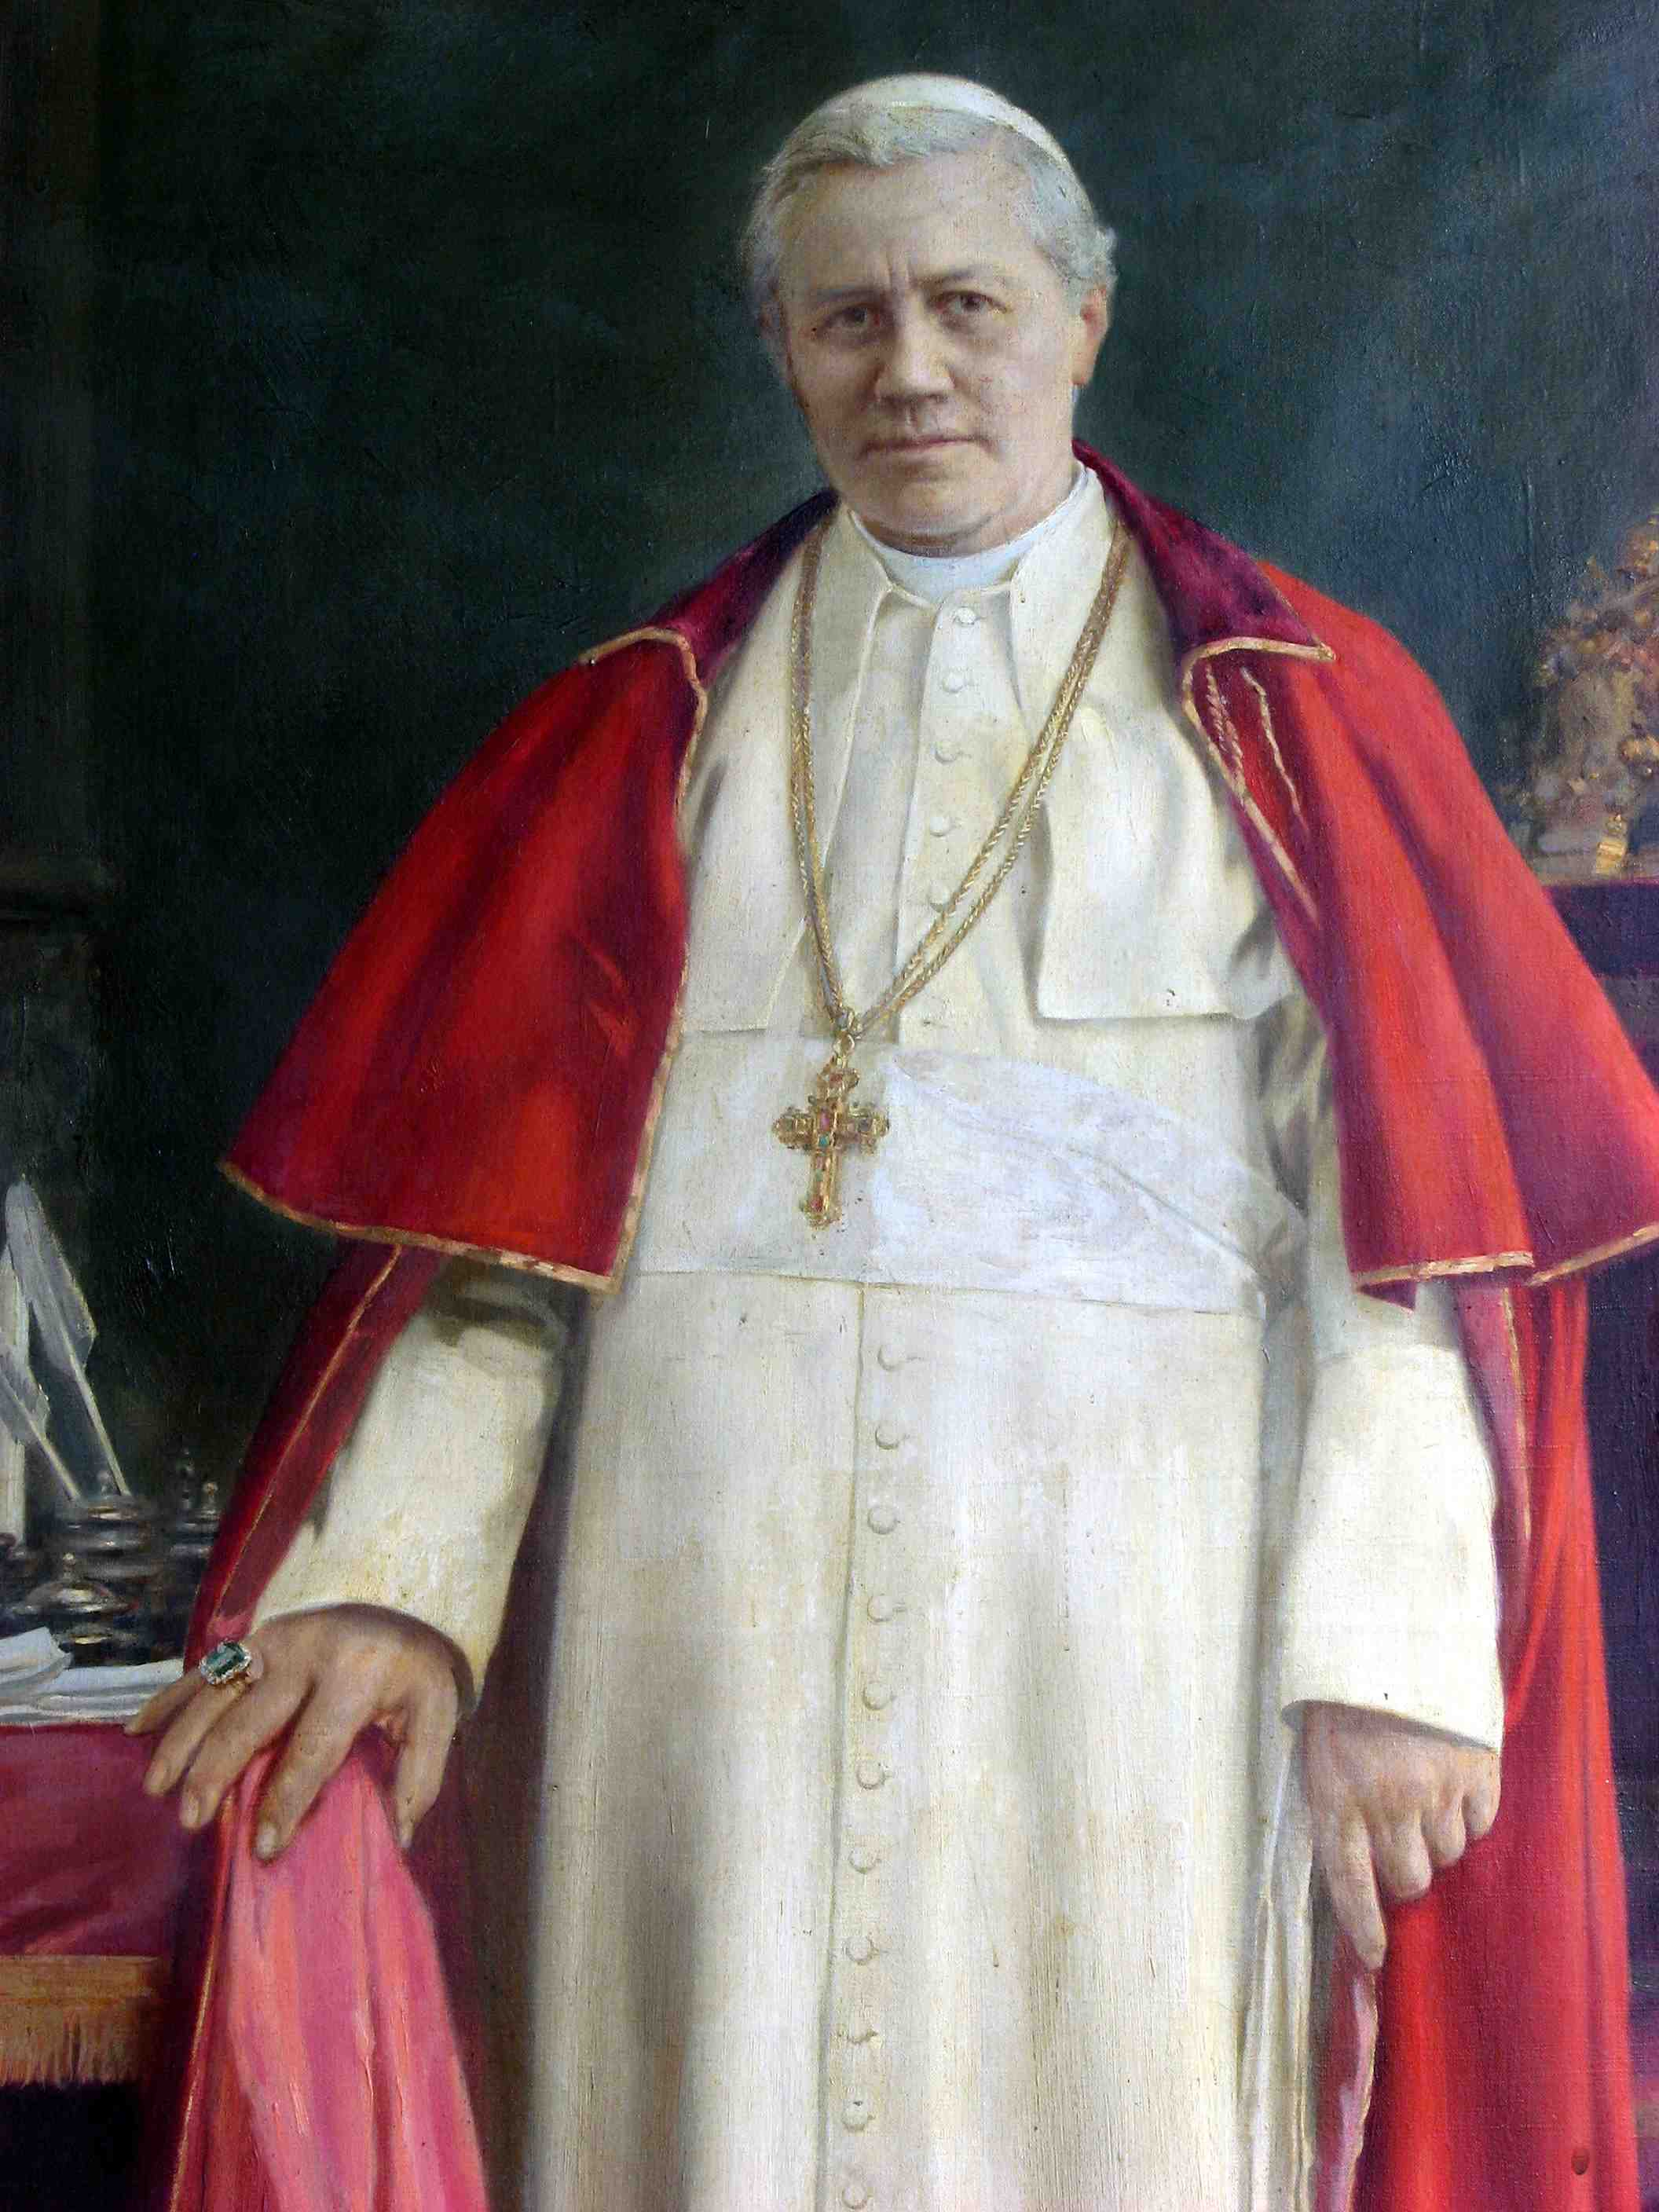
\includegraphics[width=0.5\textwidth]{media/piox}
\end{wrapfigure}
O cristão, podendo, deveria todos os dias: 1º. Assistir com devoção à Santa Missa; 2º. Fazer uma visita, por breve que fosse, ao Santíssimo Sacramento; 3º. Rezar o terço do Santo Rosário.\par
Antes do trabalho, convém oferecê-lo a Deus, dizendo do coração: «Senhor, eu Vos ofereço este trabalho, dai-me a vossa bênção». Deve-se trabalhar para glória de Deus e para fazer a sua vontade. Antes da refeição, convém fazer o sinal da Cruz, estando de pé, e depois dizer com devoção: «Senhor, abençoai-nos a nós e ao alimento que vamos tomar, para nos conservarmos no vosso santo serviço». Depois da refeição, convém fazer o sinal da Cruz, e dizer: «Senhor, eu Vos dou graças pelo alimento que me destes; fazei-me digno de participar da mesa celeste».\par
Quando nos vemos atormentados por alguma tentação, devemos invocar com fé o Santíssimo Nome de Jesus ou de Maria, ou recitar fervorosamente alguma oração jaculatória, como, por exemplo: «Dai-me a graça, Senhor, de que eu nunca Vos ofenda»; ou então fazer o sinal da Cruz, evitando, porém, que as outras pessoas, pelos sinais externos, suspeitem da tentação. Quando uma pessoa reconhece ou receia ter cometido algum pecado, convém fazer imediatamente um acto de contrição, e procurar confessar-se quanto antes. Quando fora da igreja se ouve o sinal de elevação da Hóstia na Missa solene, ou da bênção do Santíssimo Sacramento é bom fazer, ao menos com o coração, um acto de adoração, dizendo, por exemplo: «Graças e louvores se dêem a todo o momento ao Santíssimo e diviníssimo Sacramento».\par
Ao toque das Ave-Marias pela manhã, ao meio-dia e à noite, o bom cristão recita o Anjo do Senhor «Angelus» com três Ave-Marias. À noite, antes de se deitar, convém pôr-se, como de manhã, na presença de Deus, recitar devotamente as mesmas orações, fazer um breve exame de consciência, e pedir perdão a Deus dos pecados cometidos durante o dia. Antes de adormecer, farei o sinal da Cruz, pensarei que posso morrer esta noite, e oferecerei o coração a Deus, dizendo: «Meu Senhor e meu Deus, eu Vos dou todo meu coração. Trindade Santíssima, concedei-me a graça de bem viver e de bem morrer. Jesus, Maria e José, eu Vos encomendo a minha alma».\par
No decurso do dia pode-se invocar a Deus frequentemente com as orações breves que se chamam «jaculatórias». Eis algumas:\par
«Senhor, valei-me»;\par
«Senhor, seja feita vossa santíssima vontade»;\par
«Meu Jesus, eu quero ser todo vosso»;\par
«Meu Jesus, misericórdia»;\par
«Doce Coração de Jesus, que tanto nos amou, fazei que eu Vos ame cada vez mais»;\par
«Doce Coração de Maria, sede minha salvação»;\par
É muito útil recitar, durante o dia, muitas jaculatórias, e podem recitar-se também com o coração, sem preferir palavras, caminhando, trabalhando, \&c. Além das orações jaculatórias, o cristão deveria exercitar-se na «mortificação cristã». Mortificar-se quer dizer privar-se, por amor a Deus, daquilo que agrada, e aceitar o que desagrada aos sentidos ou ao amor-próprio. Quando é o Santíssimo Sacramento levado a um enfermo, devemos, sendo possível, acompanhá-Lo com modéstia e recolhimento; e, se não é possível acompanhá-Lo, fazer um acto de adoração em qualquer lugar que nos encontremos, e dizer: «Consolai, Senhor, este enfermo, e concedei-lhe a graça de se conformar com vossa Santíssima vontade e de conseguir a sua salvação».\par
Ao tocar o sino pela agonia de algum moribundo, irei, se puder, à igreja orar por ele; e, não podendo, encomendarei a Nosso Senhor a sua alma, pensando que dentro em breve hei de encontrar-me também eu nesse estado. Ao ouvir sinais pela morte de alguém, procurarei rezar um «De profundis» ou um «Réquiem», ou um Pai-Nosso e uma Ave-Maria, pela alma desse defunto, e renovarei o pensamento da morte.

%%%%%%%%%%%%%%%%%%%%CATECISMO%%%%%%%%%%%%%%%%%%%%
\newpage\section{Juramento Anti-Modernista}\label{juramentoantimodernista}

\begin{paracol}{2}\latim{
Ego {\redx N.} firmiter amplector ac recipio omnia et singula, quæ ab inerranti Ecclesiæ magisterio definita, adserta ac dedarata sunt, præsertim ea doctrinæ capita, quæ huius temporis erroribus directo adversantur.
}\switchcolumn\portugues{
Eu, {\redx N.}, firmemente aceito e creio em todas e em cada uma das verdades definidas, afirmadas e declaradas pelo magistério infalível da Igreja, sobretudo aqueles princípios doutrinais que contradizem directamente os erros do tempo presente.
}\switchcolumn*\latim{
Ac primum quidem: Deum, rerum omnium principium et finem, naturali rationis lumine per ea quæ facta sunt (Rom 1, 20), hoc est, per visibilia creationis opera, tamquam causam per effectus, certo cognosci, ideoque demonstrari etiam posse, profiteor.
}\switchcolumn\portugues{
Primeiro: creio que Deus, princípio e fim de todas as cousas, pode ser conhecido com certeza e pode também ser demonstrado, com as luzes da razão natural, nas obras por Ele realizadas (Cf. Rm I 20), isto é, nas criaturas visíveis, como (se conhece) a causa pelos seus efeitos.
}\switchcolumn*\latim{
Secundo: externa revelationis argumenta, hoc est facta divina, in primisque miracula et prophetias admitto et agnosco tamquam signa certissima divinitus ortæ Christianæ religionis, eademque teneo ætatum omnium atque hominum, etiam huius temporis, intellegentiæ esse maxime accommodata.
}\switchcolumn\portugues{
Segundo: admito e reconheço as provas exteriores da revelação, isto é, as intervenções divinas, e sobretudo os milagres e as profecias, como sinais certíssimos da origem sobrenatural da razão cristã, e as considero perfeitamente adequadas a todos os homens de todos os tempos, inclusive aquele no qual vivemos.
}\switchcolumn*\latim{
Tertio: firma pariter fide credo Ecclesiam, verbi revelati custodem et magistram, per ipsum verum atque historicum Christum, cum apud nos degeret, proxime ac directo institutam eamdemque super Petrum, apostolicæ hierarchiæ principem, ejusque in ævum successores ædificatam.
}\switchcolumn\portugues{
Terceiro: com a mesma firme fé creio que a Igreja, guardiã e mestra da palavra revelada, foi instituída imediatamente e directamente pelo próprio Cristo verdadeiro e histórico, enquanto vivia entre nós, e que foi edificada sobre Pedro, chefe da hierarquia eclesiástica, e sobre os seus sucessores através dos séculos.
}\switchcolumn*\latim{
Quarto: fidei doctrinam ab apostolis per orthodoxos patres eodem sensu eademque semper sententia ad nos usque transmissam, sincere recipio; ideoque prorsus reicio hæreticum commentum evolutionis dogmatum, ab uno in alium sensum transeuntium, diversum ab eo, quem prius habuit Ecclesia; pariterque damno errorem omnem quo divino deposito, Christi sponsæ tradito ab eaque fideliter custodiendo, sufficitur philosophicum inventum, vel creatio humanæ conscientiæ, hominum conatu sensim efformatæ et in posterum indefinito progressu perficiendæ.
}\switchcolumn\portugues{
Quarto: acolho sinceramente a doutrina da fé transmitida a nós pelos apóstolos através dos padres ortodoxos, sempre com o mesmo sentido e igual conteúdo, e rejeito totalmente a fantasiosa heresia da evolução dos dogmas de um significado a outro, diferente daquele que a Igreja professava primeiro; condeno de igual modo todo o erro que pretenda substituir o depósito divino confiado por Cristo à Igreja, para que o guardasse fielmente, por uma hipótese filosófica ou uma criação da consciência que se tivesse ido formando lentamente mediante esforços humanos e contínuo aperfeiçoamento, com um progresso indefinido.
}\switchcolumn*\latim{
Quinto: certissime teneo ac sincere profiteor, fidem non esse cæcum sensum religionis e latebris «subconscientiæ» erumpentem, sub pressione cordis et inflexionis voluntatis moraliter informatæ, sed verum assensum intellectus veritati extrinsecus acceptæ ex auditu, quo nempe, quæ a Deo personali, creatore ac Domino nostro dicta, testata et revelata sunt, vera esse credimus, propter Dei auctoritatem summe veracis.
}\switchcolumn\portugues{
Quinto: estou absolutamente convencido e sinceramente declaro que a fé não é um cego sentimento religioso que emerge da obscuridade do subconsciente por impulso do coração e inclinação da vontade moralmente educada, mas um verdadeiro assentimento do intelecto a uma verdade recebida de fora pela pregação, pelo qual, confiantes na sua autoridade supremamente veraz, nós cremos tudo aquilo que, pessoalmente, Deus, criador e senhor nosso, disse, atestou e revelou.
}\switchcolumn*\latim{
Me etiam, qua par est reverentia, subicio totoque animo adhæreo damnationibus, declarationibus, præscriptis omnibus, quæ in encyclicis litteris Pascendi et in decreto Lamentabili continentur, præsertim circa eam quam historiam dogmatum vocant.
}\switchcolumn\portugues{
Submeto-me também com o devido respeito, e de todo o coração adiro a todas as condenações, declarações e prescrições da encíclica Pascendi e do decreto Lamentabili, particularmente acerca da dita história dos dogmas.
}\switchcolumn*\latim{
Idem reprobo errorem affirmantium, propositam ab Ecclesia fidem posse historiæ repugnare, et catholica dogmata, quo sensu nunc intelleguntur, cum verioribus Christianæ religionis originibus componi non posse.
}\switchcolumn\portugues{
Reprovo outrossim o erro de quem sustenta que a fé proposta pela Igreja pode ser contrária à história, e que os dogmas católicos, no sentido que hoje lhes é atribuído, são inconciliáveis com as reais origens da razão cristã.
}\switchcolumn*\latim{
Damno quoque ac reicio eorum sententiam, qui dicunt Christianum hominem eruditiorem induere personam duplicem, aliam credentis, aliam historici, quasi liceret historico ea retinere, quæ credentis fidei contradicant, aut præmissas adstruere, ex quibus consequatur, dogmata esse aut falsa aut dubia, modo hæc directo non denegentur.
}\switchcolumn\portugues{
Desaprovo também e rejeito a opinião de quem pensa que o homem cristão mais instruído se reveste da dupla personalidade do crente e do histórico, como se ao histórico fosse lícito defender teses que contradizem a fé o crente ou fixar premissas das quais se conclui que os dogmas são falsos ou dúbios, desde que não sejam positivamente negados.
}\switchcolumn*\latim{
Reprobo pariter eam Scripturæ sanctæ diiudicandæ atque interpretandæ rationem, quæ, Ecclesiæ traditione, analogia fidei et apostolicæ Sedis normis posthabitis, rationalistarum commentis inhæret, et criticam textus velut unicam supremamque regulam haud minus licenter quam temere amplectitur.
}\switchcolumn\portugues{
Condeno igualmente aquele sistema de julgar e de interpretar a sagrada Escritura que, desdenhando a tradição da Igreja, a analogia da fé e as normas da Sé apostólica, recorre ao método dos racionalistas e com desenvoltura não menos que audácia, aplica a crítica textual como regra única e suprema.
}\switchcolumn*\latim{
Sententiam præterea illorum reiicio, qui tenent, doctori disciplinæ historicæ theologicæ tradendæ aut iis de rebus scribenti seponendam prius esse opinionem ante conceptam sive de supernaturali origine catholicæ traditionis, sive de promissa divinitus ope ad perennem conservationem uniuscuiusque revelati veri; deinde scripta patrum singulorum interpretanda solis scientiæ principiis, sacra qualibet auctoritate seclusa eaque iudicii libertate, qua profana quævis monumenta solent investigari.
}\switchcolumn\portugues{
Refuto ainda a sentença de quem sustenta que o ensinamento de disciplinas histórico-teológicas ou quem delas trata por escrito deve inicialmente prescindir de qualquer ideia pré-concebida, seja quanto à origem sobrenatural da tradição católica, seja quanto à ajuda prometida por Deus para a perene salvaguarda de cada uma das verdades reveladas, e então interpretar os textos patrísticos somente sobre as bases científicas, expulsando toda autoridade religiosa, e com a mesma autonomia crítica admitida para o exame de qualquer outro documento profano.
}\switchcolumn*\latim{
In universum denique me alienissimum ab errore profiteor, quo modernistæ tenent in sacra traditione nihil inesse divini, aut, quad longe deterius, pantheistico sensu illud admittunt, ita ut nihil iam restet nisi nudum factum et simplex, communibus historice factis æquandum: hominum nempe sua industria, solertia, ingenio scholam a Christo ejusque apostolis inchoatam per subsequentes ætates continuantium.
}\switchcolumn\portugues{
Declaro-me enfim totalmente alheio a todos os erros dos modernistas, segundo os quais na sagrada tradição não há nada de divino ou, pior ainda, admitem-no, mas em sentido panteísta, reduzindo-o a um evento pura e simplesmente análogo àqueles ocorridos na história, pelos quais os homens com o próprio empenho, habilidade e engenho prolongam nas eras posteriores a escola inaugurada por Cristo e pelos apóstolos.
}\switchcolumn*\latim{
Proinde fidem patrum firmissime retineo et ad extremum vitæ spiritum retinebo, de charismate veritatis certo, quad est, fuit eritque semper in episcopatus ab apostolis successione, non ut id teneatur, quod melius et aptius videri possit secundum suam cuiusque ætatis culturam, sed ut numquam aliter credatur, numquam aliter intellegatur absoluta et immutabilis veritas ab initio per apostolos prædicata.
}\switchcolumn\portugues{
Mantenho, portanto, e até o último suspiro manterei a fé dos pais no carisma certo da verdade, que esteve, está e sempre estará na sucessão do episcopado aos apóstolos, não para que se assuma aquilo que pareça melhor e mais consoante à cultura própria e particular de cada época, mas para que a verdade absoluta e imutável, pregada no princípio pelos apóstolos, não seja jamais crida de modo diferente nem entendida de outro modo.
}\switchcolumn*\latim{
Hæc omnia spondeo me fideliter, integre sincereque servaturum et inviolabiliter custoditurum, nusquam ab us sive in docendo sive quomodolibet verbis scriptisque deflectendo. Sic spondeo, sic iuro, sic me Deus adiuvet, et hæc sancta Dei Evangelia.
}\switchcolumn\portugues{
Empenho-me em observar tudo isto fielmente, integralmente e sinceramente, e em guardá-lo inviolavelmente, sem jamais disso me separar nem no ensinamento nem em género algum de discursos ou de escritos. Assim prometo, assim juro, assim me ajudem Deus e esses santos Evangelhos de Deus.
}\end{paracol}
\newpage\section{Verdades da Fé}

\subsubsection{Os dez mandamentos}

1 - Adorar a Deus e amá-Lo sobre todas as cousas.
2 - Não invocar o santo nome de Deus em vão.
3 - Santificar os domingos e festas de guarda.
4 - Honrar pai e mãe (e os outros legítimos superiores).
5 - Não matar (nem causar outro dano, no corpo ou na alma, a si mesmo ou ao próximo).
6 - Guardar castidade nas palavras e nas obras.
7 - Não furtar (nem injustamente reter ou danificar os bens do próximo).
8 - Não levantar falsos testemunhos (nem de qualquer outro modo faltar à verdade ou difamar o próximo).
9 - Guardar castidade nos pensamentos e nos desejos.
10 - Não cobiçar as cousas alheias.

\subsubsection{Os dous mandamentos de caridade}

\rlettrine{A}{marás} o Senhor teu Deus, com todo teu coração, com toda tua alma e com toda tua mente; Amarás ao próximo como a ti mesmo.

\subsubsection{A regra de ouro}

Tudo quanto quiserdes que os homens vos façam, fazei-lho vós também.

\subsubsection{Os cinco preceitos da Igreja}

1 - Participar na Missa, aos domingos e festas de guarda e abster-se de trabalhos e actividades que impeçam a santificação desses dias.
2 - Confessar os pecados ao menos uma vez cada ano.
3 - Comungar o sacramento da Eucaristia ao menos pela Páscoa.
4 - Guardar a abstinência e jejuar nos dias determinados pela Igreja.
5 - Contribuir para as necessidades materiais da Igreja, segundo as possibilidades.

\subsubsection{Sacramentos}

Baptismo; Confirmação; Eucaristia; Penitência ou Confissão; Extrema Unção; Ordem; Matrimónio.

\subsubsection{As Bem-Aventuranças}

\blettrine{B}{em-aventurados} os pobres em espírito, porque deles é o reino dos céus. Bem-aventurados os que choram, porque serão consolados. Bem-aventurados os mansos, porque possuirão a terra. Bem-aventurados os que têm fome e sede de justiça, porque serão saciados. Bem-aventurados os misericordiosos, porque alcançarão misericórdia. Bem-aventurados os puros de coração, porque verão a Deus. Bem-aventurados os pacificadores, porque serão chamados filhos de Deus. Bem-aventurados os que sofrem perseguição por causa da justiça, porque deles é o reino dos céus. Bem-aventurados sereis quando vos insultarem, vos perseguirem e, mentindo, disserem toda a espécie de calúnias contra vós. Alegrai-vos e exultai, porque será grande a vossa recompensa nos céus.

\subsubsection{Dias de Obrigação}

\emph{Para além de todos os Domingos}
1 de Janeiro - Solenidade de Santa Maria, Mãe de Deus;
6 de Janeiro - Epifania;
19 de Março - Solenidade de São José;
Ascensão de Jesus - Quinta-feira da sexta semana da Páscoa;
Corpus Christi - Primeira quinta-feira após o Domingo da Santíssima Trindade;
29 de Junho - Solenidade dos Apóstolos São Pedro e São Paulo; 15 de Agosto - Assunção de Maria;
1 de Novembro - Dia de Todos-os-Santos;
8 de Dezembro - Imaculada Conceição de Maria;
25 de Dezembro - Natal.

\subsubsection{Trabalhos de Misericórdia}

\begin{paracol}{2}
\begin{nscenter}{\redx Corporais}\end{nscenter}
\switchcolumn
\begin{nscenter}{\redx Espirituais}\end{nscenter}
\switchcolumn*
Dar de comer a quem tem fome; Dar de beber a quem tem sede; Vestir os nus; Dar pousada aos peregrinos; Visitar os enfermos; Visitar os presos; Enterrar os mortos.
\switchcolumn
Dar bons conselhos; Ensinar os ignorantes; Corrigir os que erram; Consolar os tristes; Perdoar as injúrias; Suportar com paciência as fraquezas do nosso próximo; Rezar a Deus por vivos e defuntos.
\end{paracol}

\subsubsection{Virtudes}

\begin{paracol}{2}
\begin{nscenter}{\redx Cardeais}\end{nscenter}
\switchcolumn
\begin{nscenter}{\redx Teologais}\end{nscenter}
\switchcolumn*
Prudência; Justiça; Fortaleza; Temperança.
\switchcolumn
Fé; Esperança; Caridade.
\end{paracol}

\subsubsection{Pecados Contra o Espírito Santo}

\emph{Pecados de pura malícia, que são contrários à bondade que se atribui ao Espírito Santo.}

Desesperar da salvação; Presunção de se salvar sem merecimentos; Combater a verdade conhecida; Ter inveja das graças que Deus dá a outrem; Obstinar-se no pecado; Morrer na impenitência final.

\subsubsection{Pecados que Bradam aos Céus}

\emph{Sua malícia é tão grave e manifesta, que provoca Deus a puni-los com os mais severos castigos.}

Homicídio voluntário; Pecado impuro contra a natureza; Opressão dos pobres, principalmente órfãos e viúvas; Não pagar o salário a quem trabalha.

\subsubsection{Do Espírito Santo}

\begin{paracol}{2}
\begin{nscenter}{\redx Dons}\end{nscenter}
\switchcolumn
\begin{nscenter}{\redx Frutos}\end{nscenter}
\switchcolumn*
Sabedoria; Entendimento; Conselho; Fortaleza; Ciência; Piedade; Temor de Deus.
\switchcolumn
Amor; Alegria; Paz; Paciência; Longanimidade; Bondade; Benignidade; Mansidão; Fé; Modéstia; Continência; Castidade.
\end{paracol}

\begin{paracol}{2}
\subsubsection{Pecados Capitais}
\switchcolumn
\subsubsection{Virtudes Opostas}
\switchcolumn*
Soberba; Avareza; Luxúria; Ira; Gula; Inveja.
\switchcolumn
Humildade; Caridade; Castidade; Paciência; Temperança; Bondade.
\end{paracol}

\subsubsection{Novíssimos}

\begin{paracol}{2}
Mors; Iudicium; Infernus; Paradisus.
\switchcolumn
Morte; Juízo; Inferno; Paraíso.
\end{paracol}

\subsubsection{Assuntos para Meditação Diária}

\begin{paracol}{2}
Deum glorificare; Jesum imitari; Beatissimam Virginem et Sanctos venerari; Angelos invocare; Animam salvare; Corpus mortificare; Virtutes a Deo exorare; Peccata expiare; Paradisum comparare; Infernum evitare; Aeternitatem considerare; Tempus bene applicare; Proximum ædificare; Mundum formidare; Dæmones impugnare; Passiones frenare; Mortem semper exspectare; Ad iudicium te præparare.
\switchcolumn
Deus para glorificar; Jesus para imitar; A abençoada Virgem e os Santos para venerar; Os Anjos para invocar; A alma para salvar; O corpo para mortificar; Virtudes para conquistar; Pecados para expiar; O paraíso para ganhar; O inferno para evitar; Eternidade para preparar; Tempo para bem aproveitar; O próximo para edificar; O mundo para desprezar; Demónios para combater; Paixões para refrear; A morte sempre esperar; E o julgamento para se preparar.
\end{paracol}

%%%%%%%%%%%%%%%%%%%%ORAÇÕES A DEUS%%%%%%%%%%%%%%%%%%%%
\newpage\section{Santíssima Trindade}\label{trindade}

\emph{Gloria na página \pageref{gloria}, Te Deum na pagina \pageref{tedeum}, Cântico dos Três Jovens na página \pageref{benedicite}.}

\subsection{Abandono à Divina Providência}

\blettrine{A}{doro-Vos} Deus Pai, que me criastes, adoro-Vos Filho, que me resgatastes, adoro-Vos Espírito Santo que tantas vezes me tendes santificado e me santificais ainda: consagro-Vos este dia por vosso amor e para vossa maior glória. Não sei o que me há-de acontecer hoje, se acaso serão sucessos penosos, se agradáveis! Passarei o dia triste ou alegre, terei consolações ou angústias? Será o que for de vosso agrado, abandono-me à vossa providência e submeto-me à vossa divina vontade. Amen.

\subsection{Santíssima Trindade pelo Anjo de Portugal}\label{fatimatrindade}
\rlettrine{S}{antíssima} Trindade, Pai, Filho e Espírito Santo, adoro-Vos profundamente e ofereço-Vos o Preciosíssimo Corpo, Sangue, Alma e Divindade de Nosso Senhor Jesus Cristo, presente em todos os sacrários da terra, em reparação dos ultrajes, sacrilégios e indiferenças com que Ele mesmo é ofendido. E, pelos méritos infinitos doseu Santíssimo Coração e do Coração Imaculado de Maria, peço-Vos a conversão dos pobres pecadores.

\begin{nscenter}\includegraphics[width=.7\textwidth, keepaspectratio]{media/pdf/cc/santissimatrindade2}\end{nscenter}
\newpage\section{Deus Pai}

\rlettrine{G}{ravai,} ó meu Deus, a vossa lei no fundo do meu coração, fazei-me conhecer os vossos santos mandamentos, e dai-me a graça de os amar e a força de os praticar.

\subsection{Benedictus Deus}\label{benedictusdeus}
\begin{paracol}{2}\latim{
\rlettrine{B}{enedíctus} Deus, et Pater Dómini nostri Jesu Christi, Pater misericordiárum, et Deus totíus consolationis, qui consolátur nos in omni tribulatióne nostra.
}\switchcolumn\portugues{
\rlettrine{B}{endito} seja Deus, e Pai de nosso Senhor Jesus Cristo, Pai de misericórdias e Deus de todas as consolações, O qual nos consola em toda nossa tribulação.
}\switchcolumn*\latim{
Deo grátias.
}\switchcolumn\portugues{
Graças a Deus.
}\end{paracol}

\subsection{Súscipe Dómine}\label{suscipedomine}
\begin{paracol}{2}\latim{
\rlettrine{S}{úscipe,} Dómine, universam meam libertatem. Accipe memoriam, intellectum atque voluntatem omnem. Quidquid habeo vel possideo mihi largitus es; id tibi totum restituo, ac tuæ prorsus voluntati trado gubernandum. Amorem tui solum cum grátia tua mihi dones, et dives sum satis, nec aliud quidquam ultra posco. Amen.
}\switchcolumn\portugues{
\rlettrine{T}{omai,} Senhor e recebei toda minha liberdade, a minha memória, o meu entendimento e toda minha vontade, tudo o que tenho e possuo; Vós mo destes; a Vós, Senhor, o restituo. Tudo é vosso, disponde de tudo, à vossa inteira vontade. Dai-me o vosso amor e graça, que esta me basta. Amen.
}\end{paracol}

\subsectioninfo{De São Francisco Xavier}{Para a conversão dos infiéis}
\begin{paracol}{2}\latim{
\rlettrine{Æ}{térne} rerum omnium effector Deus, memento abs te animas infidelium procreatas, easque ad imaginem et similitúdinem tuam conditas. Memento Jesum, Fílium tuum, pro illorum salúte atrocissimam subiisse necem.
Noli, quæso, Dómine, ultra permittere, ut Filius tuus ab infidelibus contemnatur, sed precibus sanctórum virorum et Ecclesiæ, sanctissimi Fílii tui Sponsæ, placatus, recordare misericórdiæ tuæ et, oblitus idololatriæ et infidelitatis eorum, effice ut ipsi quoque agnoscant aliquando quem misisti Dóminum Jesum Christum, qui est salus, vita et resurrectio nostra, per quem salvati et liberáti sumus, cui sit glória per infinita sǽcula sæculórum. Amen.
}\switchcolumn\portugues{
\slettrine{Ó}{} Deus, eterno, autor de todas as cousas, lembrai-Vos das almas dos infiéis, formadas por Vós à vossa imagem e semelhança: vede Senhor, que, em opróbrio vosso, deles se vai enchendo o inferno. Lembrai-Vos de que vosso Filho Jesus por sua salvação padeceu uma atrocíssima morte. Não permitais Senhor, daqui em diante, que o vosso Filho seja desprezado pelos infiéis; mas pelo contrário, deixando-se aplacar pelas preces dos santos e da Igreja, Esposa do vosso santíssimo Filho, e esquecendo a sua idolatria e infidelidade, fazei que eles também venham a conhecer Aquele que enviastes, Jesus Cristo Nosso senhor, que é a salvação, vida e ressurreição nossa, por quem fomos salvos e livres, ao qual seja dada glória por infinitos séculos. Amen.
}\end{paracol}

\newpage\ilustra{media/jesus1}

\section{Jesus}

\subsection{Anima Christi}\label{animachristi}
\begin{paracol}{2}\latim{
\rlettrine{A}{nima} Christi, sanctífica me.\\
Corpus Christi, salve me.
}\switchcolumn\portugues{
\rlettrine{A}{lma} de Cristo, santificai-me.\\
Corpo de Cristo, salvai-me.
}\switchcolumn*\latim{
Sanguis Christi, inébria me.
}\switchcolumn\portugues{
Sangue de Cristo, inebriai-me.
}\switchcolumn*\latim{
Aqua láteris Christi, lava me.
}\switchcolumn\portugues{
Água do lado de Cristo, lavai-me.
}\switchcolumn*\latim{
Pássio Christi, conforta me.
}\switchcolumn\portugues{
Paixão de Cristo, confortai-me.
}\switchcolumn*\latim{
O bone Jesu, exáudi me.
}\switchcolumn\portugues{
Ó bom Jesus, ouvi-me.
}\switchcolumn*\latim{
Intra tua vúlnera abscónde me.
}\switchcolumn\portugues{
Dentro das vossas Chagas, escondei-me.
}\switchcolumn*\latim{
Ne permittas me separári a te.
}\switchcolumn\portugues{
Não permitais que de Vós me separe.
}\switchcolumn*\latim{
Ab hoste maligno defénde me.
}\switchcolumn\portugues{
Do espírito maligno, defendei-me.
}\switchcolumn*\latim{
In hora mortis meæ voca me.
}\switchcolumn\portugues{
Na hora da minha morte, chamai-me.
}\switchcolumn*\latim{
Et jube me venire ad te, ut cum Sanctis tuis laudem te in sǽcula
sæculórum.
}\switchcolumn\portugues{
E mandai-me ir para Vós, para que Vos louve com vossos Santos, por
todos os séculos.
}\switchcolumn*\latim{
Amen.
}\switchcolumn\portugues{
Amen.
}\end{paracol}

\subsection{Jesus misericordioso, tende compaixão de mim}
\qlettrine{J}{esus} Cristo, nosso Senhor, Deus de bondade e misericórdia, aqui me tendes em vossa presença, humilhado e contrito de coração; recomendo-Vos a minha hora derradeira, e a sorte que depois dela me espera.\par
Quando os meus pés imóveis me avisarem de que meu caminho neste mundo está prestes a terminar: \textit{Jesus misericordioso, tende compaixão de mim.}\par
Quando as minhas mãos, trémulas e entorpecidas, não puderem já apertar o Crucifixo e, contra a minha vontade, o deixarem cair sobre o meu leito de dor: \textit{Jesus misericordioso, tende compaixão de mim.}\par
Quando os meus olhos, apagados e amortecidos, horrorizados à vista da morte iminente, cravarem em vossa imagem seus olhares abatidos e moribundos: \textit{Jesus misericordioso, tende compaixão de mim.}\par
Quando os meus lábios, frios e trémulos, pronunciarem pela derradeira vez o vosso adorável nome: \textit{Jesus misericordioso, tende compaixão de mim.}\par
Quando o meu rosto, pálido e arroxeado, já mover à compaixão e ao susto as pessoas presentes, e os meus cabelos parados, banhados do suor da morte, derem o sinal de que se apressa o termo dos meus dias: \textit{Jesus misericordioso, tende compaixão de mim.}\par
Quando os meus ouvidos, prestes a fecharem-se para sempre às conversações dos homens, se abrirem para ouvir de vossa boca a irrevogável sentença, que decidirá a minha sorte por toda a eternidade: \textit{Jesus misericordioso, tende compaixão de mim.}\par
Quando a minha imaginação, perturbada por fantasmas horrendos e aterradores, cair em mortal angústia, e meu espírito, abalado e confuso à vista das próprias iniquidades e receoso da vossa justiça, lutar contra o anjo das trevas, que há-de querer tirar-me a esperança na vossa misericórdia e precipitar-me no abysmo do desespero: \textit{Jesus misericordioso, tende compaixão de mim.}\par
Quando o meu coração, fraco e angustiado com as dores da doença, for surpreendido pelos horrores da morte e se achar exausto e cansado com os esforços feitos para triunfar dos inimigos da minha salvação: \textit{Jesus misericordioso, tende compaixão de mim.}\par
Quando deitar as últimas lágrimas, prenúncio da minha destruição, recebei-as, ó meu Jesus, em sacrifício de expiação, para que assim morra vítima de penitência; e naquele terrível momento: \textit{Jesus misericordioso, tende compaixão de mim.}\par
Quando os parentes e amigos, apinhados ao redor de mim, se enternecerem à vista do meu lastimoso estado, e invocarem vossa misericórdia em meu favor: \textit{Jesus misericordioso, tende compaixão de mim.}\par
Quando, perdido o uso dos sentidos e apagada de toda minha vista, gemer no meio das ânsias da agonia extrema e na crise da morte: \textit{Jesus misericordioso, tende compaixão de mim.}\par
Quando os últimos impulsos do meu coração obrigarem a minha alma a sair do corpo, recebei-os como prova de um vivo anseio de ir ter convosco; e Vós: \textit{Jesus misericordioso, tende compaixão de mim.}\par
Quando a minha alma sair para sempre deste mundo, e deixar o meu corpo pálido, frio e sem vida, aceitai a destruição do meu ser como uma homenagem que desde há ofereço à vossa Divina Majestade, e naquela hora: \textit{Jesus misericordioso, tende compaixão de mim.}\par
Quando, finalmente, a minha comparecer diante de Vós e contemplar pela primeira vez o imortal esplendor da vossa Majestade, as não expulseis de vossa presença: mas dignai-Vos receber-me no seio amoroso da vossa misericórdia, para que possa cantar eternamente os vossos louvores: \textit{Jesus misericordioso, tende compaixão de mim.}\par

\subsection{Acto de Reparação}
\rlettrine{C}{om} aquele profundíssimo respeito que a Fé me inspira, ó meu Deus e meu Salvador, Jesus Cristo, verdadeiro Deus e Homem, eu Vos adoro e amo com todo o coração no Augustíssimo Sacramento do Altar, em reparação de todas as irreverências, profanações e sacrilégios que por minha desgraça tenha cometido até agora, assim como de todos os que no passado se têm feito ou possam (tal não permita Deus) fazer-se no futuro. Adoro-Vos, pois, ó meu Deus, não só pelo muito que sois digno de ser amado e adorado, mas, ao menos, conforme o que posso; e quisera poder fazê-lo com aquela perfeição de que são capazes todas as criaturas racionais. Deste modo, tenho intenção de Vos adorar agora e sempre, não só por aqueles Católicos que Vos não adoram nem amam, mas ainda em compensação da adoração que Vos devem os infiéis, os hereges, os cismáticos, os ímpios, os blasfemos, os profanadores, os idólatras, os judeus, os maometanos e todos os outros que Vos injuriam e perseguem, e pela conversão de todos eles. Ah! Sim, meu Jesus, permiti que todos Vos conheçam, adorem e amem, e Vos dêem graças a todo o momento no Santíssimo e diviníssimo Sacramento. Amen.

\subsection{Concede Mihi}
\begin{paracol}{2}\latim{
\rlettrine{C}{oncede} mihi, benignissime Jesu, grátiam tuam, ut mecum sit et mecum laboret, mecum que in finem usque persevéret.
}\switchcolumn\portugues{
\rlettrine{I}{nfinitamente} bom Jesus, eu Vos peço que me concedeis a vossa graça; fazei que ela permaneça em mim, trabalhe comigo e se mantenha comigo até ao fim.
}\switchcolumn*\latim{
Da mihi hoc semper desiderare et velle, quod tibi magis acceptum est et carius placet.
}\switchcolumn\portugues{
Concedei-me sempre a vontade e o desejo daquilo que for mais agradável e mais aceitável para Vós.
}\switchcolumn*\latim{
Tua voluntas mea sit, et mea voluntas tuam semper sequatur et optime ei concordet.
}\switchcolumn\portugues{
Que a vossa vontade seja a minha, e que minha vontade esteja sempre em conformidade com vossa.
}\switchcolumn*\latim{
Sit mihi unum velle et nolle tecum, nec aliud posse velle aut nolle, nisi quod Tu vis et nolis. Amen.
}\switchcolumn\portugues{
Fazei que tudo aquilo que eu queira ou não queira seja aquilo que Vós quereis ou não quereis. Amen.
}\end{paracol}

\subsection{Oração a Nosso Senhor dos Passos}
\slettrine{Ó}{} Jesus, Filho Unigénito de Deus e da Virgem Imaculada, que pela salvação do mundo quisestes ser condenado, traído, atado a uma coluna, conduzido como um cordeiro ao matadouro, acusado injustamente num tribunal, ferido com pancadas, saturado de opróbrios e injúrias, cuspido no rosto, barbaramente açoitado, coroado de espinhos, condenado à morte, despojado das vestes, pregado numa cruz com toda a crueldade, suspenso entre dous ladrões, vexado com fel e vinagre, abandonado em tormentosa agonia e finalmente trespassado por uma lança: por estes tormentos, Senhor, dos quais nós, indignos filhos vosso, agora com devoção, gratidão e amor nos lembramos, e pela vossa santíssima morte na cruz, livrai-nos das penas eternas do inferno e dignai-Vos conduzir-nos ao paraíso, para onde levastes convosco o bom ladrão.\par
Tende piedade de nós, Senhor, que com o Pai e o Espírito Santo viveis e reinais pelos séculos dos séculos. Amen.

\subsection{Pureza}
\rlettrine{D}{ulcíssimo} Menino Jesus, Cordeiro imaculado, cheio de bondade, misericórdia e amor! Para nos restituirdes a santa inocência, vieste do céu à terra, sofrestes pobreza e perseguições. Eu Vos agradeço e Vos amo de todo meu coração. E por vosso amor proponho hoje firmemente guardar com todo o cuidado a santa pureza do coração. Ó meu Jesus, abençoa o meu corpo, para que seja sempre um santuário de inocência e pureza. Fazei que eu evite com cuidado todo o pecado moral, tal como a uma peste contagiosa. Ó Jesus inocentíssimo e todo imaculado, pelo vosso amor e pela vossa inocência concedei-me a virtude da santa pureza, para que eu, depois da minha morte, tenha a felicidade de ver Vos no céu.

\subsection{Consagração Pessoal a Jesus Cristo}
\emph{Nos 30 dias anteriores à consagração devem-se rezar Ladainhas, o Veni Creator Spíritus e a Ave Maris Stella, deve-se ler o Santo Evangelho e a Imitação de Cristo, assim como rezar o terço.}\par

\slettrine{Ó}{} sabedoria eterna e encarnada! Ó Amabilíssimo e adorável Jesus, verdadeiro Deus e verdadeiro homem, Filho Unigénito do Pai Eterno e da sempre Virgem Maria.
Adoro-Vos profundamente, no seio e nos esplendores do vosso Pai, durante toda a eternidade, e no seio virginal de Maria, vossa Mãe digníssima, no tempo da vossa Encarnação.
Dou-Vos graças por Vos terdes aniquilado a Vós mesmo, tomando a forma de escravo, para livrar-me da cruel escravidão do demónio.
Eu Vos louvo e glorifico por Vos terdes querido submeter em tudo a Maria, vossa Mãe Santíssima, a fim de, por Ela, tornar-me vosso fiel escravo.
Entretanto, ai de mim, criatura ingrata e infiel! Não guardei os votos e promessas que tão solenemente Vos fiz no meu Baptismo. Não cumpri as minhas obrigações; não mereço ser chamado vosso filho, nem vosso escravo; e, como nada há em mim que não mereça a vossa repulsa e a vossa cólera, não ouso aproximar-me por mim mesmo da vossa Santíssima e Augustíssima Majestade.
Recorro, pois, à intercessão e à misericórdia de vossa Mãe Santíssima, que me destes por medianeira junto de Vós. É por intermédio d’Ela que espero obter de Vós a contrição e o perdão dos meus pecados, a aquisição e conservação da Sabedoria.
Ave, pois, ó Maria Imaculada, Tabernáculo Vivo da Divindade, onde a Eterna Sabedoria escondida quer ser adorada pelos anjos e pelos homens.
Ave, ó Rainha do Céu e da Terra, a cujo Império é submetido tudo o que há abaixo de Deus.
Ave, ó Seguro Refúgio dos pecadores, cuja misericórdia a ninguém despreza. Atendei ao desejo que tenho da Divina Sabedoria, e recebei, para isso, os votos e ofertas apresentados pela minha baixeza.

Eu, {\redx N.}, infiel pecador, renovo e ratifico hoje, nas vossas mãos, as promessas do meu Baptismo: renuncio para sempre a Satanás, às suas pompas e suas obras, e dou-me inteiramente a Jesus Cristo, a Sabedoria Encarnada, para o seguir, levando a minha Cruz, todos os dias da minha vida. E para lhe ser mais fiel do que até agora tenho sido, escolho-Vos hoje, ó Maria, na presença de toda a Corte Celeste, por minha Mãe e Senhora. Entrego-Vos e consagro-Vos, na qualidade de escravo, o meu corpo e a minha alma, os meus bens interiores e exteriores, e o próprio valor das minhas boas obras passadas, presentes e futuras, deixando-Vos pleno e inteiro direito de dispor de mim e de tudo o que me pertence, sem excepção alguma, segundo o vosso agrado e para maior glória de Deus, no tempo e na eternidade.
Recebei, ó Benigníssima Virgem, esta pequenina oferta da minha escravidão, em união e em honra à submissão que a Sabedoria Eterna quis ter à vossa Maternidade; em homenagem ao poder que ambos tendes sobre este vermezinho e miserável pecador; em acção de graças pelos privilégios com que largamente Vos favoreceu a Trindade Santíssima.
Protesto que quero, de hoje em diante e firmemente, como vosso verdadeiro escravo, buscar a vossa honra e obedecer-Vos em todas as cousas.
Ó Mãe Admirável, apresentai-me ao vosso amado Filho na condição de escravo perpétuo, a fim de que, tendo-me resgatado por Vós, por Vós também me receba propiciamente.
Ó Mãe de Misericórdia, concedei-me a graça de obter a Verdadeira Sabedoria de Deus, e de colocar-me, para isso, entre o número daqueles que amais, ensinais, guiais, sustentais e protegeis como filhos e escravos vossos.
Ó Virgem Fiel, tornai-me em tudo um tão perfeito discípulo, imitador e escravo da Sabedoria Encarnada, Jesus Cristo, vosso Filho, que eu chegue um dia, por vossa intercessão e a vosso exemplo, à plenitude da sua idade na Terra e da sua glória no Céu. Amen.

\subsection{Consagração ao Sagrado Coração de Jesus}
\slettrine{Ó}{} Dulcíssimo Jesus, ó Redentor do género humano, lançai um olhar sobre nós, humildemente prostrados diante do vosso Altar! Somos vossos e vossos queremos ser; e para podermos viver mais estreitamente unidos a Vós, eis que cada um de nós se consagra ao vosso Sacratíssimo Coração. Muitos, porém, já vos não conhecem; muitos, ao desprezar os vossos Mandamentos, repudiam-Vos. Ó Benigníssimo Jesus, tende piedade de uns e de outros; e atraí todos ao vosso Coração Santíssimo.\par
Ó Senhor, sede o Rei não só dos fiéis que se não distanciaram de Vós, mas também destes filhos pródigos que Vos abandonaram; fazei com que estes retornem à Casa Paterna o quanto antes para não morrerem de miséria e fome. Sede o Rei de todos os que vivem no engano do erro ou que por discordarem de Vós se separaram; chamai-os ao Porto da Verdade e da Unidade da Fé para que assim, em breve, mais não haja que um só rebanho sob um só Pastor.\par
Sede finalmente o Rei de todos os que estão envoltos nas superstições do paganismo e não recuseis tirá-los das trevas para traze-los à Luz do Reino de Deus.\par
Obtende, ó Senhor, a integridade e liberdade segura para a vossa Igreja; dai a todo o povo a tranquilidade da ordem; fazei com que de uma extremidade à outra da Terra ressoe esta única voz:\par
℣. Seja louvado este Coração do qual provém a nossa salvação!\par
℟. A Ele a Honra e a Glória por todos os séculos. Amen.

\subsection{Coroinha do Sagrado Coração de Jesus}

\rlettrine{I}{} Amorosíssimo Jesus, quando medito no vosso Santíssimo Coração e O vejo todo piedade e bondade para com os pecadores, sinto o meu coração encher-se de alegria e de confiança de que será por Vós bem acolhido. Ai de mim, quantos pecados tenho cometido!... Mas, agora, penetrado de contrição, choro-os e detesto-os, como Pedro e Madalena, por serem ofensas a Vós, ó Sumo Bem. Eu Vo-lo suplico encarecidamente, pelo vosso Santíssimo Coração. Oxalá eu antes morra do que Vos ofenda! Que eu não viva senão para Vos Amar!

\rlettrine{II}{} Bendigo o vosso humilíssimo Coração, ó meu bom Jesus, e Vos dou graças, porque ao dardes-m’O como exemplo, não só com veementes desejos me incitastes a imitá-l’O, senão que, à custa de tantas humilhações vossas, me proporcionastes e aplanastes o caminho. Como tenho sido insensato e ingrato!... Quanto me tenho extraviado!... Perdoai-me. Não mais quero ser soberbo e ambicioso; quero somente seguir-Vos com o coração humilde entre as humilhações, e alcançar a paz e a salvação. Dai-me Vós a graça para isto, e bendizei sempre o vosso pacientíssimo Coração.

\rlettrine{III}{} Ao meditar no vosso pacientíssimo Coração. ó meu Jesus, fico confundido, e Vos dou graças por tantos exemplos maravilhosos de invicto sofrimentos, que nos deixastes. Eu me arrependo da minha indigna delicadeza, que se impacienta com a menor contrariedade. Ah! meu amado Jesus, infundi no meu coração um constante e forte amor às tribulações, às cruzes, às mortificações e à penitência, a fim de que, acompanhando-Vos ao Calvário, chegue convosco à glória e alegria do Paraíso.

\rlettrine{IV}{} Que horror sinto de mim, ó meu amado Jesus, ao contemplar o vosso amantíssimo Coração e ao ver como o meu coração é tão diverso do vosso; pois eu me inquieto, agasto e lamento à menor sombra, gesto ou palavra que contrarie. Ah! Senhor, perdoai-me todos estes defeitos, e concedei-me para o futuro a graça de imitar em qualquer contrariedade a vossa inalterável mansidão e por tal modo gozar santa e perpétua paz.

\rlettrine{V}{}Ó meu amado Jesus, vencedor da morte e do inferno, entoem-se louvores ao vosso generosíssimo Coração, que bem os merece. Quanto a mim, fico confundido ao ver o meu coração tão pusilânime, que estremece com qualquer injúria. Mas não serei mais assim! De Vós imploro tanta fortaleza e valor para sofrer as injúrias, que, combatendo e vencendo na terra, possa triunfar convosco no céu!\par

\emph{Volvamo-nos para o maternal Coração de Maria S.\textsuperscript{ma}}\par

\rlettrine{P}{elas} singulares prerrogativas do vosso dulcíssimo Coração, alcançai-me, ó Maria, Mãe de Deus e minha Mãe, uma verdadeira e permanente devoção ao Santíssimo Coração de Jesus, vosso Filho; e, assim, eu cumpra fielmente os meus deveres e com alegria sirva sempre, mas especialmente hoje, nosso Senhor Jesus Cristo.\par
℣. Coração de Jesus, abrasado em amor por nós.\par
℟. Inflamai os nossos corações de amor por Vós.\par
\begin{nscenter} Oremos. \end{nscenter}
Vos suplicamos, ó Senhor, que o Divino Espírito Santo nos inflame naquele fogo que nosso Senhor Jesus Cristo do íntimo doseu Coração lançou no mundo e quis que se acendesses em labaredas por toda a parte. Ele, que vive e reina em todos os séculos dos séculos.
℟. Amen.

\newpage\section{Espírito Santo}\label{espiritosanto}

\subsection{Veni, Sancte Spíritus}\label{venisanctespiritus}
\begin{paracol}{2}\latim{
\rlettrine{V}{eni,} Sancte Spíritus! reple tuórum corda fidélium: et tui amóris in eis ignem accénde.
}\switchcolumn\portugues{
\rlettrine{V}{inde,}ó Espírito Santo, enchei os corações dos vossos fiéis e acendei neles o fogo do vosso amor.
}\switchcolumn*\latim{
℣. Emitte Spíritum tuum, et creabúntur.
}\switchcolumn\portugues{
℣. Enviai o vosso Espírito e tudo será criado.
}\switchcolumn*\latim{
℟. Et renovábis faciem terræ.
}\switchcolumn\portugues{
℟. E renovareis a face da terra.
}\switchcolumn*\latim{
\begin{nscenter} Orémus. \end{nscenter}
}\switchcolumn\portugues{
\begin{nscenter} Oremos. \end{nscenter}
}\switchcolumn*\latim{
\rlettrine{D}{eus,} qui corda fidélium Sancti Spíritus illustratióne docuísti, da nobis in eódem Spíritu recta sápere; et de ejus semper consola Tione gaudére. Per Christum Dóminum nostrum. ℟. Amen.
}\switchcolumn\portugues{
\slettrine{Ó}{} Deus, que haveis instruído os corações dos vossos fiéis com a luz do Espírito Santo, concedei-nos, segundo o mesmo Espírito, conhecer as coisas rectas e gozar sempre das suas divinas consolações. Por Cristo, Senhor Nosso. ℟. Amen.
}\end{paracol}


\subsectioninfo{Veni Sancte Spíritus, Sequência}{Pentecostes}\label{seqvenisanctespiritus}
\begin{paracol}{2}\latim{
\rlettrine{V}{eni,} Sancte Spíritus, et emítte cǽlitus lucis tuæ rádium.
}\switchcolumn\portugues{
\rlettrine{V}{inde,} ó Espírito Santo, e enviai do céu um raio da vossa luz.
}\switchcolumn*\latim{
Veni, pater páuperum, veni, dator múnerum, veni, lumen córdium.
}\switchcolumn\portugues{
Vinde, ó pai dos pobres; vinde, doador dos dons, vinde, luz dos corações.
}\switchcolumn*\latim{
Consolátor óptime, dulcis hospes ánimæ, dulce re­fri­gérium.
}\switchcolumn\portugues{
Consolador supremo, doce hóspede da alma, doce refresco.
}\switchcolumn*\latim{
In labóre réquies, in æstu tempéries, in fletu solácium.
}\switchcolumn\portugues{
No labor sois repouso, calma no ardor e consolação no pranto.
}\switchcolumn*\latim{
O lux beatíssima, reple cordis íntima tuórum fidélium.
}\switchcolumn\portugues{
Ó beatíssima luz, enchei o íntimo os corações dos vossos fiéis.
}\switchcolumn*\latim{
Sine tuo númine, nihil est in hómine, nihil est innóxium.
}\switchcolumn\portugues{
Sem a vossa assistência nada há bom no homem, nada de inocente.
}\switchcolumn*\latim{
Lava quod est sórdidum, riga quod est áridum, sana quod est sáucium.
}\switchcolumn\portugues{
Lavai, pois, o que está sujo, regai o que está seco, curai o que está doente.
}\switchcolumn*\latim{
Flecte quod est rígidum, fove quod est frígidum, rege quod est dévium.
}\switchcolumn\portugues{
Dobrai o que é rígido, aquecei o que está frio, guiai o que está errante.
}\switchcolumn*\latim{
Da tuis fidélibus, in te con­fi­dén­tibus, sacrum sep­te­nárium.
}\switchcolumn\portugues{
Dai aos fiéis, que em Vós confiam, os sete dons sagrados.
}\switchcolumn*\latim{
Da virtútis méritum, da salútis éxitum, da perénne gáudium.
}\switchcolumn\portugues{
Dai o mérito da virtude, dai um fim feliz, dai a perene alegria.
}\end{paracol}

\subsectioninfo{Veni Creator}{Página \label{venicreator}}

\subsection{Ao Espírito Santo}
\slettrine{Ó}{} Deus clementíssimo, escutai com piedade as nossas súplicas e iluminai o nosso coração com a graça do Espírito Santo, para que mereçamos servir com dignidade os vossos mystérios e amar-Vos com caridade eterna. Ó Deus, que conheceis o nosso coração e a nossa vontade, e que não ignorais nenhum segredo: purificai os nossos pensamentos infundindo-nos o Espírito Santo, para que mereçamos amar-Vos com perfeição e louvar-Vos dignamente. Senhor, inflamai as nossas entranhas e o nosso coração com o fogo do Espírito Santo, para que Vos sirvamos com um corpo casto e Vos agrademos com um coração limpo. Nós Vos pedimos, Senhor, que o Paráclito que procede de Vós ilumine o nosso entendimento e nos leve a conhecer a verdade, como o vosso Filho nos prometeu. Nós Vos pedimos, Senhor, que nos assista o poder do Espírito Santo, para que purifique com clemência os nossos corações e nos defenda de todos os perigos. Ó Deus, que instruístes os corações dos fiéis com a luz do Espírito Santo, concedei-nos amar, no mesmo Espírito, o que é recto, e gozar sempre a sua consolação. Nós Vos pedimos, Senhor, que purifiqueis as nossas consciências para que, ao vir o nosso Senhor Jesus Cristo, vosso Filho, encontre preparada em nós a sua mansão. Ele que vive e reina convosco pelos séculos dos séculos. Amen.

\ilustracont{media/spiritus}

%%%%%%%%%%%%%%%%%%%%SANTOS%%%%%%%%%%%%%%%%%%%%
\newpage\ilustra{media/maria1}

\section{Santa Maria}

\subsection{Augusta Rainha dos Anjos}

\rlettrine{A}{ugusta} Rainha dos Anjos, Vós que recebestes de Deus o poder e a missão de esmagar a cabeça de Satanás, humildemente Vos rogamos que envieis as Legiões Celestes para que às vossas ordens persigam e combatam os demónios por toda a parte, refreando a sua audácia e precipitando-os no abismo.\par
Quem é como Deus? Ó Bondosa e Carinhosa Mãe, Vós sereis sempre o nosso amor e a nossa esperança.\par
Ó divina Mãe, enviai os Santos Anjos em nossa defesa, afastando para longe de nós o cruel inimigo.\par
Santos Anjos e Arcanjos, defendei-nos e guardai-nos. Amen.\par

\subsection{Consagração a Nossa Senhora}

\begin{paracol}{2}\latim{
\rlettrine{D}{omina} mea!\\
O Mater mea!
}\switchcolumn\portugues{
\slettrine{Ó}{} Senhora, minha!\\
Ó minha Mãe!
}\switchcolumn*\latim{
Tibi me totum offero, atque, ut me tibi probem devotum, consecro tibi hodie oculos meos, aures meas, os meum, cor meum, plane me totum.
}\switchcolumn\portugues{
Eu me ofereço todo a Vós e em prova da minha devoção para convosco Vos consagro neste dia os meus olhos, os meus ouvidos, a minha boca, o meu coração e inteiramente todo meu ser.
}\switchcolumn*\latim{
Quóniam itaque tuus sum, o bona Mater, serva me, defende me ut rem et possessionem tuam. Amen.
}\switchcolumn\portugues{
E porque assim sou todo vosso, ó incomparável Mãe, guardai-me e defendei-me como coisa e propriedade vossa. Amen.
}\end{paracol}

\subsection{Rainha do Santo Rosário}

\slettrine{Ó}{} Imaculada Rainha do Santo Rosário. Virgem Maria, Mãe de Deus e Mãe nossa, lembrai-Vos das vossas antigas promessas feitas aos nossos antepassados e dos triunfos que por Vós eles conseguiram. Pelo vosso Rosário, ó Maria, eles conservaram íntegras a fé e a religião do seu baptismo, venceram os hereges, inimigos da nossa Pátria e permaneceram fiéis à santa Igreja Católica.\par
O erro quer corromper a verdade da nossa fé cristã e católica. Ó Rainha do Santo Rosário, defendei e guarda as nossas crenças puras de todo o erro.\par
O espírito do mal quer corromper as tradições cristãs das nossas famílias e os costumes santos que a nossa religião Católica nos inspira e pede.\par
Ó Rainha do Santo Rosário, amparai e conservai o nosso espírito cristão e defendei-nos das venenosas infiltrações do espírito do mal.\par
Sede nosso amparo, nossa Rainha e nossa Mãe; nós Vos invocaremos, louvaremos, serviremos e amaremos pelo Rosário, seremos fiéis em rezar as suas dezenas e media. Seus mistérios amaremos, serviremos a Jesus e pela vossa intercessão, ó Virgem Imaculada conseguiremos a graça e o amor de Deus e nos salvaremos para sempre. Amen.\par
Rainha do Santíssimo Rosário, protegei-nos.\par
S. Domingos de Gusmão, rogai por nós.\par

\subsection{Tota Púlchra es, Maria}

\begin{paracol}{2}\latim{
℣. Tota púlchra es, Maria.
}\switchcolumn\portugues{
℣. Toda sois formosa, ó Maria.
}\switchcolumn*\latim{
℟. Tota púlchra es, Maria.
}\switchcolumn\portugues{
℟. Toda sois formosa, ó Maria.
}\switchcolumn*\latim{
℣. Et mácula originalis non est in te.
}\switchcolumn\portugues{
℣. E mácula original não há em Vós.
}\switchcolumn*\latim{
℟. Et mácula originális non est in te.
}\switchcolumn\portugues{
℟. E mácula original não há em Vós.
}\switchcolumn*\latim{
℣. Tu, gloria Jerusalem.
}\switchcolumn\portugues{
℣. Vós sois a glória de Jerusalém.
}\switchcolumn*\latim{
℟. Tu, lætitia Israël.
}\switchcolumn\portugues{
℟. Vós a alegria de Israel.
}\switchcolumn*\latim{
℣. Tu, honorificentia populi nostri.
}\switchcolumn\portugues{
℣. Vós a honra do nosso povo.
}\switchcolumn*\latim{
℟. Tu, advocata peccatorum.
}\switchcolumn\portugues{
℟. Vós a advogada dos pecadores.
}\switchcolumn*\latim{
℣. O Maria.
}\switchcolumn\portugues{
℣. Ó Maria.
}\switchcolumn*\latim{
℟. O Maria.
}\switchcolumn\portugues{
℟. Ó Maria.
}\switchcolumn*\latim{
℣. Virgo prudentissima.
}\switchcolumn\portugues{
℣. Virgem prudentíssima.
}\switchcolumn*\latim{
℟. Mater clementissima.
}\switchcolumn\portugues{
℟. Mãe clementíssima.
}\switchcolumn*\latim{
℣. Ora pro nobis.
}\switchcolumn\portugues{
℣. Rogai por nós.
}\switchcolumn*\latim{
℟. Intercede pro nobis ad Dominum Jesum Christum.
}\switchcolumn\portugues{
℟. Intercedei por nós a Nosso Senhor Jesus Cristo.
}\switchcolumn*\latim{
℣. In conceptione tua, Immaculata fuisti.
}\switchcolumn\portugues{
℣. Vós fostes, ó Virgem, Imaculada em vossa Conceição.
}\switchcolumn*\latim{
℟. Ora pro nobis Patrem cujus Filium peperisti.
}\switchcolumn\portugues{
℟. Rogai por nós ao Pai, cujo Filho destes à luz.
}\switchcolumn*\latim{
℣. Domina, protege orationem meam.
}\switchcolumn\portugues{
℣. Protegei, Senhora, a minha oração.
}\switchcolumn*\latim{
℟. Et clamor meus ad te veniat.
}\switchcolumn\portugues{
℟. E chegue até vós o meu clamor.
}\switchcolumn*\latim{
\begin{nscenter} Orémus. \end{nscenter}
}\switchcolumn\portugues{
\begin{nscenter} Oremos. \end{nscenter}
}\switchcolumn*\latim{
\rlettrine{S}{ancta} Maria, regina cælorum, mater Domini nostri Jesu Christi, et mundi domina, quæ nullum derelinquis, et nullum despicis: respice me, domina, clementer oculo pietatis, et impetra mihi apud tuum dilectum Filium cunctorum veniam peccatorum: ut qui nunc tuam sanctam et immaculatam conceptionem devoto affectu recolo, æternæ in futurum beatitudinis, bravium capiam, ipso, quem virgo peperisti, donante Domino nostro Jesu Christo: qui cum Patre et Sancto Spiritu vivit et regnat, in Trinitate perfecta, Deus, in sæcula sæculorum. ℟. Amen.
}\switchcolumn\portugues{
\rlettrine{S}{anta} Maria, Rainha dos céus, Mãe de nosso Senhor Jesus Cristo e Senhora do mundo, que a ninguém desamparais nem desprezais; ponde, Senhora, em mim os olhos da vossa piedade e alcançai-me do vosso amado Filho o perdão de todos meus pecados, para que, venerando agora afectuosamente a vossa Imaculada Conceição, mereça na outra vida a coroa da eterna bem-aventurança: por mercê d’Aquele que vós, virgem, destes à luz, Jesus Cristo, Senhor nosso, que com o Pai e o Espírito Santo vive e reina em Trindade perfeita, Deus pelos séculos dos séculos. ℟. Amen.
}\end{paracol}

\subsection{Memoráre}\label{memorare}

\begin{paracol}{2}\latim{
\blettrine{M}{emoráre,} O piíssima Virgo Maria, non esse auditum a sæculo, quemquam ad tua currentem præsidia, tua implorantem auxilia, tua petentem suffragia, esse derelictum. Ego tali animatus confidéntia, ad te, Virgo Vírginum, Mater, curro, ad te venio, coram te gemens peccátor assisto. Noli, Mater Verbi, verba mea despícere; sed audi propitia et exáudi. Amen.
}\switchcolumn\portugues{
\blettrine{L}{embrai-Vos,} ó piíssima Virgem Maria, que jamais se ouviu dizer que algum dos que têm recorrido à vossa protecção, implorado a vossa assistência, e reclamado o vosso socorro, fosse por Vós desamparado. Animado eu de tal confiança, a Vós recorro, Virgem das virgens, minha Mãe, a Vós venho, pecador gemendo perante Vós. Minhas súplicas, ó Mãe do Verbo, não desprezeis, mas ouvi-as propiciamente e atendei-me. Amen.
}\end{paracol}

\subsection{Sub tuum præsídium}\label{subtuumpræsidium}

\begin{paracol}{2}\latim{
\rlettrine{S}{ub} tuum præsídium confúgimus, sancta Dei Génetrix; nostras deprecatiónes ne despícias in necessitátibus; sed a perículis cunctis líbera nos semper, Virgo gloriósa et benedícta. Amen.
}\switchcolumn\portugues{
\slettrine{À}{} vossa protecção recorremos, Santa Mãe de Deus; não desprezeis as nossas súplicas em nossas necessidades; mas livrai-nos sempre de todos os perigos, ó Virgem gloriosa e bendita. Amen.
}\end{paracol}

\newpage\section{Orações a São José}\label{oracoessaojose}


\subsection{Oração a São José pelo Papa Leão XIII}\label{saojose}
\begin{paracol}{2}\latim{
\rlettrine{A}{d} te beáte Joseph, in tribulatióne nostra confúgimus, atque, imploráto Sponsæ tuæ sanctíssimæ auxílio, patrocínium quoque tuum fidenter expóscimus. Per eam, quǽsumus, quæ te cum immaculáta Vírgine Dei Genitríce coniúnxit, caritátem, perque patérnum, quo Púerum Jesum ampléxus es, amórem, súpplices deprecámur, ut ad hereditátem, quam Jesus Christus acquisívit Sánguine suo, benígnus respícias, ac necessitátibus nostris tua virtúte et ope succúrras. Tuére, o Custos providentíssime divínæ Famíliæ, Jesu Christi sóbolem eléctam; próhibe a nobis, amantíssime Pater, omnem errórum ac corruptelárum luem; propítius nobis, sospítator noster fortíssime, in hoc cum potestáte tenebrárum certámine e cælo adésto; et sicut olim Púerum Jesum e summo eripuísti vitre discrímine, ita nunc Ecclesiam sanctam Dei ab hostílibus insídiis atque ab omni adversitáte défende: nosque síngulos perpétuo tege patrocínio, ut ad tui exémplar et ope tua suffúlti, sancte vívere, pie émori, sempiternámque in cælis beatitúdinem ássequi possímus. Amen
}\switchcolumn\portugues{
\slettrine{Ó}{} Bem-aventurado S. José, a vós recorremos na nossa tribulação, e, havendo implorado da Santíssima Virgem, vossa esposa, pedimos também com toda a confiança a vossa protecção. Por aquele afecto que vos uniu à Imaculada Virgem Mãe de Deus e pelo paternal amor que consagraste ao Menino Jesus, vos rogamos e suplicamos que olheis benigno para a herança que Jesus Cristo nos adquiriu com seu sangue, e que nos assistais nas nossas necessidades com vosso poder e auxílio. Protegei, ó providentíssimo guarda da Sagrada Família, os filhos escolhidos de Jesus Cristo, preservai-nos, ó pai amantíssimo, de todo o contágio das doutrinas erróneas e de corrupção; sede-nos propício e assisti-nos do alto do céu, ó nosso poderoso libertador, neste combate contra o poder das trevas; e, assim como outrora livrastes o Menino Jesus do perigo da morte, assim também, hoje, defendei a santa Igreja de Deus das ciladas dos seus inimigos e de todas as adversidades. E a cada um de nós concedei a vossa constante protecção, a fim de que, imitando-vos e fortalecidos com vosso auxílio, possamos viver santamente, morrer piamente e alcançar no céu a bem-aventurança eterna. Amen
}\end{paracol}


\subsubsection{Oração}
\slettrine{Ó}{} glorioso S. José, Pai e protector das Virgens, guarda fiel a quem Deus confiou Jesus, a própria inocência, e Maria, Virgem das virgens! Em nome de Jesus e de Maria, este duplo tesouro que vos foi tão caro, vos suplico que me conserveis livre de toda a impureza, para que com alma pura e corpo casto, sirva sempre, fielmente, a Jesus e a Maria. Amen.

\subsection{Para o Trabalho}
\slettrine{Ó}{} glorioso S. José, modelo de todos os que se consagram ao trabalho! Alcançai-me a graça de trabalhar com espírito de penitência, em expiação dos meus pecados; de trabalhar com consciência, pondo o cumprimento do meu dever acima das minhas naturais inclinações; de trabalhar com agradecimento e alegria, olhando como uma honra o poder de desenvolver por meio do trabalho os dons recebidos por Deus. Alcançai-me a graça de trabalhar com ordem, constância, intensidade e presença de Deus, sem jamais retroceder ante as dificuldades; de trabalhar, acima de tudo, com pureza de intenção e desapego de mim mesmo, tendo sempre diante dos meus olhos todas as almas e as contas que prestarei a Deus do tempo perdido, das habilidades inutilizadas, do bem omitido e das estéreis vaidades em meus trabalhos, tão contrárias à obra de Deus. Tudo por Jesus, tudo por Maria, tudo à vossa imitação, ó Patriarca São José! Este será o meu lema na vida a na morte. Amen.

\newpage\section{Portugal}

\subsection{Anjo Custódio de Portugal}
\slettrine{Ó}{} Deus omnipotente e sempiterno, que com inefável providência destinais para cada nação um Anjo, que a guarde, concedei-nos, Vos suplicamos, que, pelas súplicas e pelo patrocínio do Anjo Custódio da nossa Nação, sejamos sempre livres de todas as adversidades. Amen.

\subsection{Os Nossos Santos}

\subsubsection{Santo Francisco e Santa Jacinta}
\begin{paracol}{2}\latim{
\rlettrine{D}{eus,} qui innocentiam diligis et humiles exaltas, da nobis, ut exemplo beatorum Francisci et Hyacinthæ, puritate cordis tibi servientes, in regnum cælorum introire mereamur. Amen.
}\switchcolumn\portugues{
\rlettrine{D}{eus} de infinita bondade, que amais a inocência e exaltais os humildes, concedei, pela intercessão da Imaculada Mãe do vosso Filho, que, à imitação dos bem-aventurados Francisco e Jacinta, Vos sirvamos em pureza de coração, para podermos entrar no reino dos Céus. Amen.
}\end{paracol}

\subsubsection{Oração a Santa Beatriz da Silva}
\begin{paracol}{2}\latim{
\rlettrine{D}{eus,} qui ad cultum Imaculatæ Virginis promovendum, beatam Beatricem Virginem singulari castitatis prærogativa decorasti, et per eam novam in Ecclesia tua familiam suscitasti; da nobis ejus intercessione et exemplo ita innocenter vivere, ut terrenis omni bus abdicatis, gaudiis perfrui mereamur æternis. Per Dominum nostrum. Amen.
}\switchcolumn\portugues{
\slettrine{Ó}{} Deus, que para promover o culto da Virgem Imaculada, adornastes a B. Beatriz com a singular prerrogativa da castidade, e fundastes por meio dela uma Ordem na vossa Igreja, concedei-nos que por sua intercessão e exemplo, vivamos tão santamente que, desprezando as coisas da terra, mereçamos desfrutar os gozos eternos. Por Nosso Senhor Jesus Cristo. Amen.
}\end{paracol}

\subsection{Santo António}

\subsubsection{Objectos Perdidos}
\blettrine{E}{u,} vos saúdo, glorioso Santo António, fiel protector dos que em vós esperam. Já que recebestes de Deus o poder especial de fazer achar os objectos perdidos, socorrei-me neste momento, a fim de que, mediante vosso auxílio, eu encontre o objecto que procuro...\par
Alcançai-me, sobretudo, uma fé viva, uma esperança firme, uma caridade ardente e uma docilidade sempre pronta aos desejos de Deus. Que eu me não detenha apenas nas coisas deste mundo. Saiba valorizá-las e utilizá-las como algo que nos foi emprestado e lute sobretudo por aquelas coisas que ladrão nenhum pode nos arrebatar e nem iremos perder jamais. Amen.

\subsubsection{Responsório de Santo António}\label{respstantonio}

\begin{paracol}{2}\latim{
\rlettrine{S}{i} quæris mirácula, mors, error, calámitas, dæmon, lepra fúgiunt, ægri surgunt sani.
}\switchcolumn\portugues{
\rlettrine{S}{e} milagres procurais, a morte, o erro, a calamidade, o demónio, e a lepra fogem, os enfermos saudáveis se levantam.
}\switchcolumn*\latim{
\emph{Ant.} Cedunt mare, víncula: membra, resque pérditas, pétunt et accípiunt juvénes et cani.
}\switchcolumn\portugues{
\emph{Ant.} Cede o mar embravecido, recupera-se o perdido, pedem e recebem, tanto velhos como mancebos.
}\switchcolumn*\latim{
Péreunt perícula, cessat et necéssitas, narrent hi qui séntiunt, dicant Paduáni.
}\switchcolumn\portugues{
Desaparecem os perigos e cessa a indigência, digam-no aqueles que o sentiram, e digam-no os Paduanos.
}\switchcolumn*\latim{
\emph{Ant.} Cedunt mare, víncula: membra, resque pérditas, pétunt et accípiunt juvénes et cani.
}\switchcolumn\portugues{
\emph{Ant.} Cede o mar embravecido, recupera-se o perdido, pedem e recebem, tanto velhos como mancebos.
}\switchcolumn*\latim{
Glória Patri et Fílio et Spirítui Sancto.
}\switchcolumn\portugues{
Glória ao Pai, e ao Filho e ao Espírito Santo.
}\switchcolumn*\latim{
\emph{Ant.} Cedunt mare, víncula: membra, resque pérditas, pétunt et accípiunt juvénes et cani.
}\switchcolumn\portugues{
\emph{Ant.} Cede o mar embravecido, recupera-se o perdido, pedem e recebem, tanto velhos como mancebos.
}\switchcolumn*\latim{
℣. Ora pro nobis, beate Antoni.
}\switchcolumn\portugues{
℣. Rogai por nós, bem-aventurado António.
}\switchcolumn*\latim{
℟. Ut digni efficiamur promissionibus Christi.
}\switchcolumn\portugues{
℟. Para que sejamos dignos das promessas de Cristo.
}\switchcolumn*\latim{
\begin{nscenter} Orémus. \end{nscenter}
}\switchcolumn\portugues{
\begin{nscenter} Oremos. \end{nscenter}
}\switchcolumn*\latim{
\rlettrine{E}{cclesiam} tuam, Deus, beati Antonii Confessoris tui atque Doctoris solemnitas votiva lætificet, ut spiritualibus semper muniatur auxiliis, et gáudiis perfrui mereatur æternis. Per Christum Dóminum nostrum. ℟. Amen.
}\switchcolumn\portugues{
\slettrine{Ó}{} Deus, nós Vos suplicamos, que alegre à vossa Igreja a solenidade votiva do bem-aventurado Santo António, vosso Confessor e Doutor, para que, fortalecida sempre com os espirituais auxílios, mereça gozar os prazeres eternos. Por Jesus Cristo, Nosso Senhor. ℟. Amen.
}\end{paracol}

\subsection{Portuguesa Nação Nossa}

\subsubsection{Oração a Nossa Senhora de Fátima}
\blettrine{V}{irgem} Imaculada, que pelo vosso Santo Rosário extinguistes outrora no seio da Igreja a nefasta heresia dos albigenses, por ele libertastes a cristandade do perigo muçulmano e robustecestes a piedade dos fiéis, extingui também no povo português, pela prática mais intensa da vossa devoção, os gérmenes de morte que fazem definhar a sua Fé, libertai-o de todos os perigos internos e externos que ameaçam a pureza dos seus costumes, fortalecei-o mais e mais, fazendo rejuvenescer nele o genuíno espírito de piedade que no Passado o fez um povo cristianíssimo, fidelíssimo e evangelizador.\par
E já que, por uma inefável prova de celestial predilecção, Vos dignastes visitar este povo que se ufana de ser vassalo vosso, mostrando-lhe dos montes da Fátima quão caro é ao vosso Coração, não deixeis nunca, Mãe amorosíssima, de o acalentar com esse mesmo amor de predilecção. Descansai sobre ele olhares de misericórdia, fazei-lhe sentir mais e mais a vossa suavíssima protecção e os doces atractivos do vosso Coração, que é coração de mãe.\par
Abençoai, ó Virgem Imaculada, a terra que Vos dignastes visitar, atraí a Vós todos os portugueses, patenteai-lhes os tesouros do vosso amor, revelai-lhes os arcanos do vosso Coração materno, fazei de cada coração português um órgão que vibre de amor por Vós e de Portugal inteiro um santuário de amor que corresponda com seu filial afecto ao vosso carinho maternal; e assim mereça agora e sempre ser chamado a Terra de Santa Maria. Amen.

\subsubsection{Exército de Almas}
\rlettrine{M}{ajestade} Divina, Senhor da vida e da morte, dos que Vos amam e dos que Vos perseguem! Por intercessão da Santíssima Virgem de Fátima, Rainha da Paz e nossa Mãe, Vos pedimos que não deixeis a nossa Pátria onde Maria ergueu seu trono, venha a ser dominada e destruída por obra dos vossos inimigos. Enviai os vossos Santos Anjos a todos os locais da nossa terra e permiti que eles possam desenvolver as suas potências em todos seus recantos, para que o inimigo não venha a triunfar na nossa Pátria. Nós queremos formar um exército de almas que rezam para que Vós, Deus Uno e Trino, estendais a vossa Mão poderosa sobre este povo que é de Maria vossa Mãe. Permiti, ó Deus, que as nuvens tempestuosas que pairam sobre a humanidade e tendem a espalhar-se e a submergir a nossa Pátria, sejam afastadas. Só Vós podeis salvar-nos! Pela vossa graça e especial protecção da nossa Padroeira Maria Imaculada e do Anjo Custódio de Portugal, permiti, ó Deus, que a nossa terra nunca seja aniquilada pelo inimigo. Deus Santo, Deus Forte, Deus Todo-Poderoso, Deus Imortal, em união com todos os Santos Anjos, pedimo-Vos auxílio e Bênção para a nossa Pátria, por Jesus Cristo Nosso Senhor. Amen.

\subsubsection{Rocha sobre a qual a nossa nação se fundou}
\rlettrine{S}{enhor} Pai santo, confiamos o nosso Portugal à vossa misericórdia e protecção. Vós sois a rocha sobre a qual a nossa nação se fundou. Só Vós sois a fonte da verdade e do amor. Reclamai esta terra para a vossa glória e habitai no meio do vosso povo. Enviai o vosso Espírito e tocai os corações dos líderes da nossa nação. Abri os seus corações ao grande valor da vida humana e às responsabilidades que acompanham a liberdade humana. Relembrai o vosso povo que a verdadeira felicidade está enraizada na procura e no cumprimento da vossa vontade. Por intercessão de Maria Imaculada. Padroeira da nossa terra, concedei-nos a coragem de levar o Evangelho do vosso Filho Jesus a todos aqueles com quem convivemos e de o testemunhar com uma vida santa. Por Cristo Nosso Senhor. Amen.

\subsection{Oração de Desagravo}
\slettrine{Ó}{} Cruz adorável do meu amantíssimo Jesus!... Como vós sois bela!... Como vós faleis ao meu pobre coração!...\par
De vós pendeu o meu Deus feito homem por meu amor!... Pregado em vós deu-me até à última gota o sangue preciosíssimo do seu coração!... Em vós morreu, e como morreu!..., o meu Jesus!...\par
E desde então, ó Cruz bendita, vós ficastes sendo a nossa maior glória, ficastes sendo a nossa vida, o nosso amparo e consolação.\par
Feliz o homem, que nas agruras deste exilio se deixa guiar por vós! Felizes as nações, que vos tomam por norte, ó Cruz do meu Senhor!...\par
E, no entanto, há quem vos esqueça, há quem vos ultraje e quem vos ofenda, e, nos dias tristes que vamos atravessando, há até quem vos derrube, quem vos calque aos pés!...\par
E nem sequer a estes insultos vos poupam neste vosso querido Portugal!...\par
Neste Portugal, que vós abençoastes no berço com tanto amor; neste Portugal, que dominou os mares, porque vós lhe guiastes as caravelas; neste Portugal, que assombrou o mundo com seus feitos, porque vós, ó Cruz, lhe destes como a ninguém heroicidade e valor!...\par
E eu que sou português, e que vos amo, não hei-de cair a vossos pés para reparar tantas ingratidões?!...\par
Perdoai-lhes, oh!, perdoai-lhes e iluminai-os para que vejam o abismo que com vosso desprezo estão cavando, vejam o terrível futuro que sem vós estão preparando para este pobre Portugal!...\par
Perdoai-lhes e que todos vos amem, ó Cruz da minha alma, ó Cruz do meu Jesus!...\par
E, se para ser ouvido é necessário um sacrifício, eu, aqui estou por vós pronto para tudo, contando que me salveis e salveis Portugal. Amen.

\newpage\section{Fátima}

\subsection{Meu Deus pelo Anjo de Portugal}
\rlettrine{M}{eu} Deus! Eu creio, adoro, espero e amo-Vos. Peço-Vos perdão para os que não crêem, não adoram, não esperam e não Vos amam!

\subsectioninfo{Santíssima Trindade pelo Anjo de Portugal}{Página \pageref{fatimatrindade}}

\subsection{Nossa Senhora aos Santos Pastorinhos}\label{omeujesus}
\begin{paracol}{2}\latim{
℣. Oh mi Jesu, dimitte nobis débita nostra, líbera nos ab igne inférni,
}\switchcolumn\portugues{
℣. Ó meu Jesus, perdoai-nos e livrai-nos do fogo do inferno,
}\switchcolumn*\latim{
℟. Conduc in cælum omnes animas, præsértim illas quæ máxime indigent misericórdia tua.
}\switchcolumn\portugues{
℟. Levai as alminhas todas para o Céu e socorrei principalmente as que mais precisarem.
}\end{paracol}


\subsection{Imaculado Coração de Maria}
\slettrine{Ó}{} Jesus, é por vosso amor, pela conversão dos pecadores e em reparação pelos pecados cometidos contra o Imaculado Coração de Maria!

\subsection{Santíssimo Sacramento}
\slettrine{Ó}{} Santíssima Trindade, eu Vos adoro. Meu Deus, meu Deus, eu Vos amo no Santíssimo Sacramento.

\subsection{Avé de Fátima}
\rlettrine{A}{vé,} Avé, Avé Maria! Avé, Avé, Avé Maria!\\
A Virgem Maria, Cercada de luz, Nossa Mãe bendita, E Mãe de Jesus.\\
Foi aos pastorinhos, Que a Virgem falou, Desde então nas almas, Nova luz brilhou.\\
Com doces palavras, Mandou-nos rezar, A Virgem Maria, Para nos salvar.\\
Mas jamais esqueçam, Nossos corações, Que nos fez a Virgem, Determinações.\\
Falou contra o luxo, Contra o impudor, De modestas modas, De uso pecador.\\
Disse que a pureza, Agrada a Jesus, Disse que a luxúria, Ao fogo conduz.\\
A treze de Outubro, Foi o seu adeus, E a Virgem Maria, Voltou para os céus.\\
À Pátria que é vossa, Senhora dos Céus, Dai honra, alegria, E a graça de Deus.\\
À Virgem bendita, Cante seu louvor, Toda nossa terra, Um hino de amor.\\
Todo o mundo a louve, Para se salvar, Desde o vale ao monte, Desde o monte ao mar.\\
Ah! Demos-Lhe graças, Por nos dar seu bem, À Virgem Maria, Nossa querida Mãe!\\
E para pagarmos, Tal graça e favor, Tenham nossas almas, Só bondade e amor.\\
Avé, Virgem Santa, Estrela que nos guia, Avé, Mãe Pátria. Oh! Virgem Maria!\\

\subsection{Hino dos Pastorinhos}
\rlettrine{C}{antemos,} alegres, a uma só voz: Francisco e Jacinta rogai por nós.\\
Salve, salve, Pastorinhos, Nosso encanto e alegria, Salve, salve, pastorinhos, Predilectos de Maria, vossos olhos inocentes, Contemplaram a Senhora, Dos seus filhos peregrinos, Carinhosa protectora, Sacrifício e oração, Foi a vossa vida inteira, Ao convite maternal, Da Senhora da azinheira.\\
Praticando a caridade, Entregáveis com carinho, A merenda que leváveis, Ao primeiro pobrezinho, Caminhantes neste mundo, Ajudai-nos, cada dia, A viver sempre seguros, Sob o manto de Maria, A Senhora do Rosário, Pela vossa intercessão, Abençoe o Santo Padre, E nos leve à conversão.\\
Contemplando Deus no Céu, Pelos anjos adorado, Alcançai o dom da paz, Para o mundo extraviado.\\
Protegei a nossa Pátria, Para que, à sombra da cruz, Guarde sempre a fé cristã, E a verdade de Jesus.

\newpage\section{Orações Diversas}

\subsection{Pro Summo Pontifice}
\begin{paracol}{2}\latim{
℣. Orémus pro Pontífice nostro {\redx N.}
}\switchcolumn\portugues{
℣. Oremos pelo nosso Pontífice {\redx N.}
}\switchcolumn*\latim{
℟. Dóminus consérvet eum, et vivíficet eum, et beátum fáciat eum in terra, et non tradat eum in ánimam inimicórum ejus.
}\switchcolumn\portugues{
℟. Que o Senhor o conserve e vivifique, que o faça santo na terra e o não entregue à vontade dos seus inimigos.
}\switchcolumn\portugues{
℟. Pater Noster... Ave Maria...
}\switchcolumn\portugues{
℟. Pai Nosso... Ave Maria...
}\switchcolumn\portugues{
℟. Deus, ómnium fidélium pastor et rector, fámulum tuum {\redx N.}, quem pastórem Ecclésiæ tuæ præésse voluísti, propítius réspice: da ei, quǽsumus, verbo et exémplo, quibus præest, profícere: ut ad vitam, una cum grege sibi crédito, pervéniat sempitérnam. Per Christum, Dóminum nostrum. Amen.
}\switchcolumn\portugues{
℟. Ó Deus, pastor e guia de todos os fieis, olhai misericordiosamente sobre vosso Servo {\redx N.} que escolheestes para pastor da vossa Igreja; concedei-lhe que, com sua palavra e exemplo, encaminhe o rebanho que lhe confiastes, e juntamente com ele, possa alcançar a vida eterna. Por Cristo Senhor nosso. Amen.
}\end{paracol}

\subsection{Prece a São Miguel Arcanjo}\label{precesaomiguel}
\begin{paracol}{2}\latim{
\rlettrine{P}{rinceps} gloriosíssime cæléstis militiæ, sancte Michaël Archangele, defénde nos in prælio advérsus príncipes et potestátes, advérsus mundi rectóres tenebrárum harum, contra spirituália nequitiæ, in cæléstibus.
}\switchcolumn\portugues{
\rlettrine{G}{loriosíssimo} Príncipe da Milícia Celeste, São Miguel Arcanjo, defendei-nos «no nosso combate contra os principados e potestades, contra os príncipes do mundo tenebroso, contra as hostes espirituais da iniquidade nas regiões celestes».
}\switchcolumn*\latim{
Veni in auxilium hominum; quos Deus ad imáginem similitúdinis suæ fecit, et a tyránnide diáboli emit prétio magno.
}\switchcolumn\portugues{
Vinde em auxílio dos homens, que Deus criou à sua imagem e semelhança e que remiu, por alto preço, da tirania do demónio.
}\switchcolumn*\latim{
Te custódem et patrónum sancta venerátur Ecclésia; tibi trádidit Dóminus ánimas redemptórum in supérna felicitáte locándas. Deprecáre Deum pacis, ut cónterat sátanam sub pédibus nostris, ne ultra váleat captivos tenére hómines, et Ecclésiæ nocére.
}\switchcolumn\portugues{
A Santa Igreja vos venera como Guarda e Patrono, a vós, Deus confiou as almas remidas destinadas a ter assento na suprema Felicidade. Rogai ao Deus da Paz que esmague Satanás debaixo dos nossos pés, que ele não possa mais reter os homens cativos e infligir males à Igreja.
}\switchcolumn*\latim{
Offer nostras preces in Conspéctu Altíssimi, ut cito anticipent nos misericórdiæ Dómini, et apprehéndas dracónem, serpéntem antiquum, qui est diábolus et sátanas, et ligátum mittas in abyssum, ut non sedúcat ámplius gentes.
}\switchcolumn\portugues{
Oferecei as nossas preces ao Altíssimo, a fim de que, sem demora, possa atrair a sua misericórdia sobre nós; prendei «o dragão, a antiga serpente que é o Diabo e Satanás», lançai-o acorrentado no abysmo, «que ele mais não possa seduzir as nações».
}\end{paracol}

\subsection{Ao Anjo da Guarda}
\subsubsection{Ángele Dei}\label{angeledei}
\begin{paracol}{2}\latim{
\slettrine{Á}{ngele} Dei, qui custos es mei, me, tibi commíssum pietáte supérna, illúmina, custódi, rege et gubérna. Amen.
}\switchcolumn\portugues{
\rlettrine{S}{anto} Anjo do Senhor, meu zeloso guardador, pois que a ti me confiou a piedade divina, hoje e sempre me governa, rege, guarda e ilumina. Amen.
}\end{paracol}

\subsection{Fidelíssimo Companheiro}
\rlettrine{M}{eu} fidelíssimo companheiro, a quem Deus destinou para minha guarda, protector e defensor meu, muitas graças Vos dou por me haverdes livrado de tantos perigos; guiai-me no caminho do céu, preservai-me de todo o pecado e de toda desgraça: apresentai à divina Majestade as minhas orações e obras pias, os meus trabalhos e aflições, e fazei que em graça passe desta à vida eterna. Amen.

\subsection{Oração Universal do Papa Clemente XI}
\begin{paracol}{2}\latim{
\blettrine{C}{redo} Domine, sed credam firmius; spero, sed sperem securius; amo, sed amem ardentius; doleo, sed doleam vehementius.
}\switchcolumn\portugues{
\blettrine{S}{enhor,} creio em Vós, fazei que creia com mais firmeza; espero em Vós, fazei que espere com mais confiança; amo-Vos, aumentai o meu amor; arrependo-me, avivai a minha dor.
}\switchcolumn*\latim{
Adoro te ut primum principium; desidero ut finem ultimum; laudo ut benefactorem perpetuum; invoco ut defensorem propitium.
}\switchcolumn\portugues{
Adoro-Vos como primeiro princípio; desejo-Vos como último fim; exalto-Vos como benfeitor perpétuo; invoco-Vos como defensor propício.
}\switchcolumn*\latim{
Tua me sapientia dirige, iustitia contine, clementia solare, potentia protege.
}\switchcolumn\portugues{
Dirigi-me com vossa sabedoria; atai-me com vossa justiça; consolai-me com vossa clemência; protegei-me com vosso poder.
}\switchcolumn*\latim{
Offero tibi, Domine cogitanda, ut sint ad te; dicenda, ut sint de te; facienda, ut sint secundum te; ferenda, ut sint propter te.
}\switchcolumn\portugues{
Ofereço-Vos os meus pensamentos, para que se dirijam a Vós; minhas palavras, para que falem de Vós; minhas obras, para que sejam vossas; minhas contrariedades, para que as aceite por Vós.
}\switchcolumn*\latim{
Volo quidquid vis, volo quia vis, volo quomodo vis, volo quamdiu vis.
}\switchcolumn\portugues{
Quero o que quereis, quero porque o quereis, quero como o quereis, quero enquanto o queirais.
}\switchcolumn*\latim{
Oro, Domine, intellectum illumines, voluntatem inflammes, cor emundes, animam sanctifices.
}\switchcolumn\portugues{
Senhor, peço-Vos que ilumineis a minha mente, inflameis a minha vontade, limpeis o meu coração, santifiqueis a minha alma.
}\switchcolumn*\latim{
Defleam praeteritas iniquitates, repellam futuras tentationes, corrigam vitiosas propensiones, excolam idoneas virtutes.
}\switchcolumn\portugues{
Que me afaste das faltas passadas, rejeite as tentações futuras, corrija as más inclinações, pratique as virtudes necessárias.
}\switchcolumn*\latim{
Tribue mihi, bone Deus, amorem tui, odium mei, zelum proximi, contemptum mundi.
}\switchcolumn\portugues{
Concedei-me, Deus de bondade, amor por Vós, ódio por mim, zelo pelo próximo, desprezo pelo mundano.
}\switchcolumn*\latim{
Studeam superioribus oboedire, inferioribus subvenire, amicis consulere, inimicis parcere.
}\switchcolumn\portugues{
Que saiba obedecer aos superiores, ajudar os inferiores, acolher os amigos, perdoar os inimigos.
}\switchcolumn*\latim{
Vincam voluptatem austeritate, avaritiam largitate, iracundiam lenitate, tepiditatem fervore.
}\switchcolumn\portugues{
Que vença a sensualidade com a mortificação, a avareza com a generosidade, a ira com a bondade, a tibieza com a piedade.
}\switchcolumn*\latim{
Redde me prudentem in consiliis, constantem in periculis, patientem in adversis, humilem in prosperis.
}\switchcolumn\portugues{
Fazei-me prudente nos conselhos, constante nos perigos, paciente nas contrariedades, humilde na prosperidade.
}\switchcolumn*\latim{
Fac, Domine, ut sim in oratione attentus, in epulis sobrius, in munere sedulus, in proposito firmus.
}\switchcolumn\portugues{
Senhor, fazei-me atento na oração, sóbrio na comida, perseverante no trabalho, firme nos propósitos.
}\switchcolumn*\latim{
Curem habere innocentiam interiorem, modestiam exteriorem, conversationem exemplarem, vitam regularem.
}\switchcolumn\portugues{
Que procure ter inocência interior, modéstia exterior, conversa exemplar, vida ordenada.
}\switchcolumn*\latim{
Assidue invigilem naturae domandae, gratiae fovendae, legi servandae, saluti promerendae.
}\switchcolumn\portugues{
Que lute por dominar a minha natureza, fomentar a graça, servir a vossa lei e obter a salvação.
}\switchcolumn*\latim{
Discam a te quam tenue quod terrenum, quam grande quod divinum, quam breve quod temporaneum, quam durabile quod aeternum.
}\switchcolumn\portugues{
Que aprenda de Vós como é pouco o terreno, como é grande o divino, como é breve o tempo, como é duradouro o eterno.
}\switchcolumn*\latim{
Da mortem praeveniam, iudicium pertineam, infernum effugiam, paradisum obtineam.
}\switchcolumn\portugues{
Fazei-me preparar a morte, temer o juízo, evitar o inferno e alcançar o Paraíso.
}\switchcolumn*\latim{
Per Christum Dominum nostrum. Amen.
}\switchcolumn\portugues{
Por Cristo Nosso Senhor. Amen.
}\end{paracol}

\subsection{Bom Humor}
\rlettrine{C}{oncedei-me,} Senhor, uma boa digestão, mas também algo para digerir. Concedei-me um corpo saudável, e o bom humor necessário para o manter. Concedei-me uma alma simples que saiba valorizar o que é bom, que se não amedronte diante do mal, e que encontre os meios para voltar a colocar as cousas no seu lugar. Dai-me uma alma que não conheça o aborrecimento, nem as murmurações, nem os suspiros, nem os lamentos, nem preocupações excessivas com esse obstáculo chamado «eu». Concedei-me, Senhor, o dom do sentido de humor. Permiti-me a graça de aproveitar o riso para que saboreie nesta vida um pouco de alegria, e possa partilhá-la com os outros. Amen.

\subsection{Oração de São Francisco}
\rlettrine{S}{enhor,} fazei de mim um instrumento da vossa paz; onde houver ódio, que eu leve o amor; onde houver ofensa, que eu leve o perdão; onde houver discórdia, que eu leve a união; onde houver dúvida, que eu leve a fé; onde houver erro, que eu leve a verdade; onde houver desespero, que eu leve a esperança; onde houver tristeza, que eu leve a alegria; onde houver trevas, que eu leve a luz. Ó Mestre, fazei que eu procure mais consolar que ser consolado, compreender que ser compreendido, amar que ser amado. Pois é dando que se recebe, é perdoando que se é perdoado, e é morrendo que se vive para a vida eterna. Amen.

\subsection{Conversão dos Pecadores}
\begin{paracol}{2}\latim{
\rlettrine{Æ}{terne} rerum omnium effector Deus, memento abs te animas infidelium procreatas, easque ad imaginem et similitudinem tuam conditas. Memento Jesum, Filium tuum, pro illorum salute atrocissimam subiisse necem. Noli, quæso, Domine, ultra permittere, ut Filius tuus ab infidelibus contemnatur, sed precibus sanctorum virorum et Ecclesiæ, sanctissimi Filii tui Sponsæ, placatus, recordare misericordiæ tuæ et, oblitus idololatriæ et infidelitatis eorum, effice ut ipsi quoque agnoscant aliquando quem misisti Dominum Jesum Christum, qui est salus, vita et resurrectio nostra, per quem salvati et liberati sumus, cui sit gloria per infinita sæcula sæculorum. Amen.
}\switchcolumn\portugues{
\rlettrine{D}{eus} eterno, Criador de todas as cousas, lembrai-Vos que as almas dos infiéis são obras de vossas mãos, e que são feitas à vossa imagem e semelhança. Vede, porém, Senhor, como em desonra do vosso Nome o inferno se enche destas almas. Lembrai-Vos que Jesus Cristo, vosso Filho, derramou todo seu Sangue e padeceu uma morte atrocíssima por elas. Não permitais, pois, Senhor, que o vosso Filho seja por mais tempo desprezado pelos infiéis. Deixai-Vos antes mover à piedade pelas orações de vossos Santos e da Igreja, esposa de vosso Santíssimo Filho. Lembrai-Vos da vossa misericórdia e, esquecendo a sua idolatria e infelicidade, fazei que também eles conheçam Jesus Cristo, Nosso Senhor, que é nossa Salvação, Vida e Ressurreição, pelo qual fomos livres e salvos do inferno, e a quem seja dado honra, glória e louvor para sempre. Amen.
}\end{paracol}

\subsection{Jaculatórias}
Meu Jesus, misericórdia!\par
Jesus, manso e humilde de coração, fazei o meu coração semelhante ao vosso.\par
Doce Coração de meu Jesus, fazei que eu Vos ame cada vez mais.\par
Seja feita, louvada e eternamente exaltada a justíssima, altíssima e amabilíssima vontade de Deus em todas as cousas.\par
Ó Maria concebida, sem pecado. Rogai por nós que recorremos a Vós.\par
Ó meu Jesus, perdoai-nos, livrai-nos do fogo do inferno. Levai as almas
todas para o Céu e socorrei principalmente as que mais precisarem\par
Ó Jesus, manso e humilde de coração, fazei o nosso coração semelhante
ao vosso.\par
Meu Deus, eu creio, adoro, espero e amo-Vos. Peço-Vos perdão para os que
não crêem, não adoram, não esperam e não Vos amam.\par
Senhor, valei-me.\par
Senhor, seja feita a vossa santíssima vontade.\par
Maria, Auxílio dos Cristãos, rogai por nós.\par
Meu Jesus, eu quero ser todo vosso.\par
Meu Jesus, misericórdia.\par
Doce Coração de Jesus, que tanto nos amais, fazei com que eu Vos ame cada vez mais.\par
Doce Coração de Maria, sede minha salvação.\par
Santa Bárbara Bendita, que no céu está escrita com papel e água benta, nos livre desta tormenta.\par
São Miguel Arcanjo, defendei-nos no combate.\par

\subsection{Cruz de S. Bento}
\begin{nscenter}

\includegraphics[width=.8\textwidth]{media/bento}
\end{nscenter}
\begin{paracol}{2}\latim{
{\redx C.S.P.B.:} Crux Sancti Patris Benedicti.
}\switchcolumn\portugues{
{\redx C.S.P.B.:} Cruz do Santo Patriarca Bento.
}\switchcolumn*\latim{
{\redx C.S.S.M.L.:} Crux Sancta Sit Mihi Lux.
}\switchcolumn\portugues{
{\redx C.S.S.M.L.:} A Cruz Santa seja a minha Luz.
}\switchcolumn*\latim{
{\redx N.D.S.M.D.:} Non Draco Sit Mihi Dux.
}\switchcolumn\portugues{
{\redx N.D.S.M.D.:} Que o Dragão não seja meu Senhor.
}\switchcolumn*\latim{
{\redx V.R.S.:} Vade Retro Satana!
}\switchcolumn\portugues{
{\redx V.R.S.:} Retira-te, Satanás!
}\switchcolumn*\latim{
{\redx N.S.M.℣.} Numquam Suades Mihi Vana!
}\switchcolumn\portugues{
{\redx N.S.M.℣.} Não me aconselhes loucuras!
}\switchcolumn*\latim{
{\redx S.M.Q.L.:} Sunt Mala Quæ Libas.
}\switchcolumn\portugues{
{\redx S.M.Q.L.:} São maldades o que me apresentas.
}\switchcolumn*\latim{
{\redx I.V.B.:} Ipse Venena Bibas.
}\switchcolumn\portugues{
{\redx I.V.B.:} Tu mesmo bebe esses venenos.
}\switchcolumn*\latim{
Amen.
}\switchcolumn\portugues{
Amen.
}\end{paracol}

\subsection{Renovação das Promessas do Baptismo}
\rlettrine{R}{enuncio} hoje a Satanás, a todas suas obras e a todas suas pompas. A Vós, meu Jesus, prometo fé e fidelidade, quero ficar fiel ao vosso amor até à morte. Afasta-te de mim, Satanás! Pertenço Jesus, e só a Jesus quero servir. Meu amabilíssimo Jesus, não permitais que hoje por algum pecado me separe de Vós.

\subsection{Requiem Æternam}\label{requiem}
\begin{paracol}{2}\latim{
\rlettrine{R}{équiem}ætérnam dona eis, Dómine, et lux perpétua lúceat eis. Requiéscant in pace. Amen.
}\switchcolumn\portugues{
\rlettrine{D}{ai-lhes,} Senhor, o eterno descanso entre os esplendores da luz perpétua. Descansem em paz. Amen.
}\end{paracol}

\subsection{Aceitação da Morte}
\rlettrine{M}{eu} Deus e meu Pai, Senhor da vida e da morte, que, para justo castigo das nossas culpas, com um decreto imutável determinastes que todos os homens haviam de morrer, olhai para mim, aqui prostrado diante de Vós. Detesto com todo o coração as minhas culpas passadas, pelas quais mereci mil vezes a morte, que aceito agora com o fim de expiá-las e para obedecer à vossa amável vontade. Gostosamente morrerei, Senhor, no momento, no lugar e do modo que Vós quiserdes, e aproveitarei até essa altura os dias que me restam de vida para lutar contra os meus defeitos e aumentar o meu amor por Vós, para quebrar os laços que atam o meu coração às criaturas, para preparar a minha alma para comparecer na vossa presença; e desde agora me abandono sem reservas nos braços da vossa paternal Providência.

\subsection{Obter uma Boa Morte}
\rlettrine{M}{eu} Criador e meu Pai, peço-Vos a mais importante das vossas graças: a perseverança final e uma morte santa. Por maior que tenha sido o abuso da vida que me destes, concedei-me a graça de vivê-la desde agora e de terminá-la no vosso santo amor. Que eu morra como os Santos Patriarcas, abandonando sem tristeza este vale de lágrimas, para ir gozar o descanso eterno na minha verdadeira pátria. Que eu morra como o glorioso S. José, acompanhado por Jesus e Maria, pronunciando estes nomes dulcíssimos, que espero bendizer por toda a eternidade. Que eu morra como a Virgem Imaculada, dentro da mais pura caridade e com o desejo de me unir ao único objecto dos meus amores. Que eu morra como Jesus na Cruz, plenamente identificado com a vontade do Pai, feito um holocausto por amor. Jesus, morto por mim, concedei-me a graça de morrer com um acto de perfeita caridade para convosco. Santa Maria, Mãe de Deus, rogai por mim agora e na hora da minha morte. S. José, meu Pai e Senhor, alcançai-me a graça de morrer com a morte dos justos.

\subsection{Momento da Morte}
\rlettrine{S}{enhor,} meu Deus, de boa vontade aceito desde já, como vinda das vossas mãos, qualquer espécie de morte que quiserdes enviar-me, com todas suas angústias, penas e dores.\par
℣. Amado Jesus, José e Maria,\par
℟. Dou-Vos o coração e a alma minha.\par
℣. Amado Jesus, José e Maria,\par
℟. Assisti-me na última agonia.\par
℣. Amado Jesus, José e Maria,\par
℟. Expire em paz entre Vós a alma minha.\par

\newpage\subsection{Terço Bernardes}\label{tercobernardes}

\begin{nscenter}
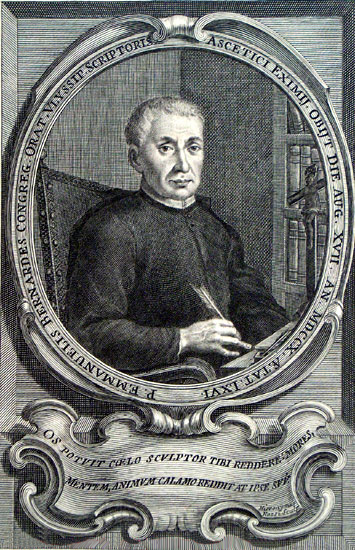
\includegraphics[width=0.5\textwidth]{media/bernardes}
\end{nscenter}

\begin{nscenter} \emph{Década 1} \end{nscenter}

Senhor Deus: eu sou a miséria, a ingratidão, a indignidade; sou um pecador vilíssimo, a quem não devia cobrir o Céu nem sustentar a Terra. Havei de mim misericórdia, e salvai-me por amor de vossa bondade.

Pai: pequei contra o Céu, e em vossa presença; não sou digno de me chamar filho vosso; fazei-me como qualquer de vossos mercenários.

Lavai-me, meu Senhor Jesus Cristo, nas correntes de vosso precioso Sangue; e limpai minha alma das manchas de todo o pecado.

Desgarrei-me como ovelha perdida. Que fora de mim, ó bom Pastor, se me não buscásseis, e tomásseis sobre vossos ombros?

Eis aqui está à vossa porta o pobre: eis aqui o leproso e cego, e tolhido, e coberto de inumeráveis chagas. Não necessitam de médico os sãos, mas os enfermos; vinde, e curai-me com vossa palavra, para glória de vosso nome.

Que era eu, Senhor, no meio de meus vícios, e fora de vossa graça, senão um cão morto, coberto das moscas dos demônios, que em minha podridão se cevavam. Vistes minha miséria, e vos apiedastes. Destes-me vida e misericórdia. Oh, bendito seja tal amor!

Inclinai, Senhor, para mim vossos amorosos olhos, e apagai meus pecados. Concedei-me a graça da renovação de meu espírito, com uma vida totalmente conforme à vossa lei.

Deus meu: proponho firmemente, com o auxílio de vossa graça, não admitir jamais ofensa vossa. Oh! não mais pecar, não mais desprezar vossos preceitos; guardá-los, sim, mais que as meninas dos meus olhos.

Senhor: alcance eu de vós esta mercê; que, no ponto em que certamente hei de cair de vossa graça, antes caia morto de repente; porque viver com injúria vossa pior morte é que a mesma morte, e maior desgraça que o inferno.

Jesus amorosíssimo, Jesus minha Redenção e remédio: de tantas lágrimas que andando neste mundo chorastes, dai-me uma para que amoleça este coração, e o derreta pelos olhos. Dai-me uma lágrima vossa, para que a apresente a vosso Eterno Padre em remissão de meus pecados.

\begin{nscenter} \emph{Década 2} \end{nscenter}

Não entreis, Senhor, em juízo com vosso servo; porque nenhum vivente se justificará diante de vós. De mil cargos que me fizerdes, não poderei responder a um só. Todo me entrego nos braços de vossa misericórdia.

Que maldade há no mundo tão execrável, que eu não esteja pronto para a cometer? Senhor, amarrai com as cadeias de vosso santo temor as fúrias de minha liberdade; porque sou capaz de tornar a crucificar-vos.

Isto me pasma, Senhor: como não respeitei vossa presença! Como não temi vossa indignação! Como me não compadeci de vossas dores! Como pisei vosso Sangue! Como não correspondi a tanto amor! Não pode haver maior cegueira.

Pecaste, alma minha: diz-me, agora, que fruto tiraste do teu pecado? Amaste as criaturas mais que ao Criador: que te ficou rendendo esta desordem? Perda da amizade de Deus, e do direito à sua glória, remorso de consciência, costume de tornar a pecar, escravidão ao demônio, reato da culpa, dívida da pena eterna. Oh, quem dera rios de lágrimas a meus olhos, para lamentar tão grave desgraça!

Vinde, vinde, Senhor, ao meu coração; formai um azorrague das cordas de vosso amor e temor, e lançai daqui todos os maus afetos que profanam a vossa casa.

Rogo-vos, meu Jesus, por aquele primeiro leite que bebeste nos peitos virginais de vossa Mãe Santíssima; e por aquelas sagradas primícias de vosso Sangue, que derramastes na Circuncisão, que não permitais que jamais caia de vossa graça nem esteja um ponto fora dela.

Pequei mais que o número das areias do mar. Porém, Senhor, as vossas misericórdias não têm número. Em vós ponho toda minha esperança: não padecerei confusão eterna.

Eu a pecar; vós, Senhor, a perdoar-me. Eu a fazer-vos injúrias; vós a fazer-me benefícios. O certo é, Senhor, que cada um obra como quem é. Bendita seja vossa paciência, que tanto me esperou.

Muito agravado estais de mim, e vos sobra razão. Oh, quem para aplacar-vos tivera as lágrimas de uma Madalena, as penitências de uma Egipcíaca, os gemidos de um Agostinho, a compunção de um S. Pedro!

Ah, pecador atrevido e infame! Tu foste o que açoutaste a JESUS, tu o que o coroaste de espinhos; o que lhe lançaste salivas no rosto, o que o pregaste na Cruz. Como te não confundes?

\begin{nscenter} \emph{Década 3} \end{nscenter}

Lembrai-vos, Senhor, que sou obra de vossas mãos; lembrai-vos que vos custei muito na Cruz. Não entregueis às bestas infernais as almas que vos confessam.

Não me dirás, alma minha, que males te fez teu Deus, para que assim o ofendesses? Acaso foi crime o morrer por ti de amor em uma Cruz? Porventura te agravou em querer salvar-te, e dar-te o Reino de sua Glória? Que razão posso dar, Senhor, do pecado, que é a mesma sem-razão? Misericórdia.

Ora pazes, Senhor; pazes para sempre; fiz mal, assim o confesso diante do Céu e da Terra. Não farei mais; perdoai-me por quem sois.

Vaidade de vaidades, e tudo vaidade. Que me pode render o amor do mundo, e todas suas cousas, senão deleite falso, que em um momento passa; tormento verdadeiro, que em uma eternidade não passa?

Que fará um desgraçado a quem a morte colheu em pecado mortal e sepultou nas profundezas? Oh, que gemidos! Oh, que ânsias! Oh, que remorsos! Oh, que desesperações! Oh, que incêndios! Tu não puderas já ser este? Quanto devo, Senhor, à vossa paciência! Bendita seja eternamente.

Não dissestes vós, Senhor, que havia grande festa e alegria no Céu quando algum pecador se convertia? Eia, amorosíssimo Jesus, fazei com vossa graça que seja eu o assunto desta alegria e festa.

Eis-me, aqui Senhor, que sou o filho pródigo, e dissipei a substância de vossa graça, e andei na região remota de vossa presença, apascentando os animais imundos de meus apetites; já torno para vossa graça, lançai-me os braços de vossa caridade.

Oh, banhe-me esse precioso Sangue, que com tanto amor derramastes pelos pecadores! Banhe-me todo com um perfeito batismo, e ficarei mais alvo que a neve.

Senhor Deus: aqui nesta vida me castigai, aqui me abrasai, contanto que me perdoeis eternamente. Não queirais, Senhor, entesourar contra mim vossa ira; não me guardeis para a outra vida a satisfação de vossa justiça.

Oh, horas preciosas dadas para servir e amar a Deus, e empregadas em ofendê-lo! Quem nunca houvera nascido para tanto mal! Ou quem de novo tornara a nascer, para o emendar!

\begin{nscenter} \emph{Década 4} \end{nscenter}

Oh, que cego andava eu Senhor, pois estava sem vós, e vós sois Luz! Oh, como ia errado, pois estava fora de vós, e vós sois Caminho! Oh, que nesciamente procedia, pois estava sem vós, e vós sois Sabedoria! Oh, como estava morto, pois estava sem vós, e vós sois vida!

Nada sou, nada valho, nada posso senão ofender-vos, e precipitar-me no inferno. Esta mesma verdade que agora conheço, se afastares vossa luz, me ficará oculta; e sobre tantas misérias minhas se acrescentará outra, de as não conhecer.

Oh, alma minha, em que te ocupas, em que te enredas? O teu Jesus coroado de espinhos, e tu de flores? Ele suando Sangue, e tu buscando refrigérios? Ele farto de opróbrios, tu faminta de honras? Oh, confusão! Mudemos de vida; tomemos a Cruz; sigamos os passos de Cristo.

De quantos bens me destes, Senhor, usei mal, e em ofensa vossa. Se me fizésseis Anjo, creio que já também fora demônio. Oh, quem tivera digno sentimento de tão enormes excessos, verdadeira dor de pecados tão graves!

O ofício que tomei, Senhor, foi o de pecar; e neste me exercitei com toda a diligência, estudando muito de propósito na maldade. Oh, que bem concordava isto com o fim para que vós me criastes, que é amar-vos, e gozar-vos eternamente! Só vós, que sois infinito em bondade, podereis sofrer tanto.

Onde me esconderei, Senhor, até que passe a vossa ira? Fugirei de vós para vós mesmo; de vós, reto Juiz, para vós, Pai clementíssimo. Em vossas chagas me recolho, que este é o sagrado que vale aos que vão fugindo à vossa justiça.

Oh, quanta foi até agora minha negligência e descuido! O tempo que me concedestes para a penitência, desperdicei-o; os auxílios de vossa graça, rejeitei-os; às vozes com que me chamáveis me fiz surdo. E agora, Senhor, que hei de fazer? Pesa-me de haver pecado; havei de mim misericórdia, misericórdia.

Que dormisse eu tão seguro sobre a vossa ofensa, pendurado do fio da vida sobre a boca do inferno! Grande temeridade a minha! Senhor, dai-me entendimento, e viverei amando-vos e servindo-vos.

Oh, se eu já desprezasse o mundo como ele merece! Oh, se metera debaixo dos pés todas as cousas terrenas! Oh, se somente fizera estimação das eternas!

Afastai, Senhor, vosso rosto de meus pecados; e apagai e extingui todas minhas iniqüidades. Criai em mim um coração novo; e renovai o espírito reto em minhas entranhas.

\begin{nscenter} \emph{Década 5} \end{nscenter}

Sei que hei de aparecer em vosso tribunal; sei que hei de dar-vos estreita conta de toda minha vida. Não me atrevo, Senhor, a suportar vossos olhos irados. Ordenai agora minha vida, de modo que não desmereça então vê-los benignos.

Aqui vos mostro, Senhor, todas minhas chagas. Vede como são muitas, como são profundas, como são envelhecidas? Ó médico Divino, sarai as minhas chagas com vossas; que, para os filhos de Adão estarem sãos, quis o Filho de Deus estar chagado.

Não te desalentes, Alma minha, com a enormidade e multidão de teus pecados. Espera sempre em Deus até à noite cerrada da tua morte; que em Deus há infinita misericórdia e redenção copiosa.

Ajudai-me, Deus Salvador meu; livrai-me por amor da glória do vosso nome. Não vos lembreis de minhas maldades; submergi-as no mar de vossa bondade imensa.

Olha, Alma minha, olha para teu Deus posto por ti em uma Cruz, eis ali o que perdoa, e apaga os teus pecados. Vê quanto padeceu por te salvar; vê com que fina caridade te ama. Guarda-te de jamais tornar a ofendê-lo.

A vós, Senhor, que sois dulcíssimo Esposo de minha alma, desprezei-vos; ao demônio, que é adúltero, fiz-lhe a vontade. Tomara morrer de sentimento de tão feia desordem. Tomara chorar de dia e de noite tão execranda maldade.

Que tenho eu com o mundo, que passa como figura? Que tenho eu com a carne, que murcha como flor? Que tenho com as cousas transitórias, que tudo é engano, perigo, trabalho, vaidade? Eia, eia, salvemos a alma nas tabuas da Cruz, fazendo penitência.

Oh, momento do qual pende a eternidade! Só quem te não considera te não teme. Abri-me, Senhor, os olhos da alma, não me suceda adormecer no letargo da morte eterna.

Senhor, aqui venho fugindo de meus inimigos: abri-me as portas de vossa misericórdia. Recolhei o vosso fugitivo, meu Deus; recolhei-me depressa, que meus inimigos me vêm ao alcance.

Dulcíssimo Jesus: o vosso soberano nome quer dizer Salvador; obrai em mim conforme vosso nome e salvai-me.


\subsectioninfo{Oração de Manassés}{Século II}\label{manasses}
\newpage\begin{paracol}{2}\latim{
Domine Deus omnipotens patrum nostrorum Abraham et Isaac et Jacob et semini eorum iusto;
}\switchcolumn\portugues{
Ó Senhor, Deus omnipotente de nossos pais, Abraão, Isaque e Jacó, e de sua justa semente;
}\switchcolumn*\latim{
Domine qui fecisti cælum et terram cum omni ornatu eorum;
}\switchcolumn\portugues{
Senhor que fizestes os céus e a terra, com todos seus adornos;
}\switchcolumn*\latim{
Qui signasti mare verbo præcepti tui, qui conclusisti abyssum et signasti eam terribili et laudabili nomine tuo;
}\switchcolumn\portugues{
Que marcastes o mar com a palavra de vosso mandamento; que prendestes nas profundezas, e o selastes com vosso temível e glorioso Nome;
}\switchcolumn*\latim{
Quem omnia pavent et tremunt a vultu virtutis tuæ,
}\switchcolumn\portugues{
Que todos Vos tenham temor, e tremam diante do vosso poder;
}\switchcolumn*\latim{
Quia importabilis est magnificentia gloriæ tuæ et insustentabilis ira super peccatores comminationis tuæ;
}\switchcolumn\portugues{
Porque ninguém pode aguentar perante a majestade da vossa glória, e a vossa ira contra os pecadores é insuportável;
}\switchcolumn*\latim{
Immensa vero et investigabilis misericordia promissionis tuæ,
}\switchcolumn\portugues{
Verdadeiramente, a vossa promessa de misericórdia é imensurável e insondável;
}\switchcolumn*\latim{
Quoniam Tu es Dominus altissimus super omnem terram benignus longanimis et multum misericors et pænitens super malitias hominum.
}\switchcolumn\portugues{
Porque Vós sois o altíssimo Senhor sobre toda a terra, de grande compaixão, paciente, muito misericordioso e lamentoso das maldades dos homens.
}\switchcolumn*\latim{
Tu, autem, Domine, secundum bonitatem tuam promisisti pænitentiam et remissionem iis qui peccaverunt tibi; et multitudine miserationum tuarum decrevisti pænitentiam peccatoribus in salutem.
}\switchcolumn\portugues{
Porém Vós, ó Senhor, de acordo com vossa grande bondade prometestes o perdão àqueles que pecaram contra Vós: e de vossas infinitas misericórdias conferistes o arrependimento aos pecadores, para que possam ser salvos.
}\switchcolumn*\latim{
Et, tu, igitur, Domine, Deus iustorum, non posuisti pænitentiam iustis Abraham et Isaac et Jacob his qui tibi non peccaverunt, sed posuisti pænitentiam propter me peccatorem.
}\switchcolumn\portugues{
Vós portanto, ó Senhor, Deus dos justos, não conferistes arrependimento aos justos, assim como a Abraão, Isaque e Jacó, que não pecaram contra Vós; mas Vós conferistes arrependimento a mim, pecador;
}\switchcolumn*\latim{
Quoniam peccavi super numerum harenæ maris, multiplicatæ sunt iniquitates meæ, Domine, multiplicatæ sunt iniquitates meæ! Et non sum dignus intueri et aspicere altitudinem cæli præ multitudine iniquitatum mearum.
}\switchcolumn\portugues{
Porque os meus pecados são mais que o número das areias do mar, multipliquei as minhas iniquidades, ó Senhor, multipliquei as minhas iniquidades! E não sou digno de contemplar os altos céus por causa da multidão das minhas iniquidades.
}\switchcolumn*\latim{
Incurvatus sum multo vinculo ferro, ut non possim attollere caput meum et non est respiratio mihi, quia excitavi iracundiam tuam et malum coram te feci statuens abominationes et multiplicans offensiones.
}\switchcolumn\portugues{
Estou preso por correntes de ferro, não posso levantar a minha cabeça, nem respirar, pois provoquei a vossa ira, e fiz o que era mau perante Vós, levantando abominações, e multiplicando ofensas.
}\switchcolumn*\latim{
Et nunc flecto genua cordis mei, precans ad te bonitatem Domine.
}\switchcolumn\portugues{
E agora dobro os joelhos e humilho o meu coração implorando a vossa graça, ó Senhor.
}\switchcolumn*\latim{
Peccavi, Domine, peccavi, et iniquitatem meam agnosco.
}\switchcolumn\portugues{
Pequei, ó Senhor, pequei, e reconheço as minhas iniquidades;
}\switchcolumn*\latim{
Quare peto rogans te, Domine, remitte mihi, remitte mihi! Ne simul perdas me cum iniquitatibus meis neque in æternum iratus reserves mala mihi neque damnes me in infima terræ loca. Quia tu es, Deus, Deus inquam pænitentium,
}\switchcolumn\portugues{
Por isso humildemente Vos imploro, perdoai-me, ó Senhor, perdoai-me! Não me destruais com as minhas iniquidades, nem fiqueis irado comigo para sempre, nem me condeneis às partes baixas da terra. Porque Vós sois Deus, o Deus dos arrependendidos;
}\switchcolumn*\latim{
Et in me ostendes omnem bonitatem tuam! Quia indignum salvabis me secundum magnam misericordiam tuam,
}\switchcolumn\portugues{
E em mim derramareis a vossa bondade! Pois indigno, salvastes-me, de acordo com vossa grande misericórdia.
}\switchcolumn*\latim{
Et laudabo te semper omnibus diebus vitæ meæ. Quoniam te laudat omnis virtus cælorum et tibi est gloria in sæcula sæculorum. Amen.
}\switchcolumn\portugues{
Por isso eu Vos louvarei em todos os dias da minha vida. Porque todos os poderes dos céus Vos louvam, e para Vós é a glória em todos os séculos. Amen.
}\end{paracol}

%%%%%%%%%%%%%%%%%%%%DIÁRIAS%%%%%%%%%%%%%%%%%%%%
\newpage\section{Orações Diárias}

\subsubsection{Sinal da Cruz}\label{sinalcruz}
\begin{paracol}{2}\latim{
\cruz In nómine Patris, et Fílii, et Spíritus Sancti. Amen.
}\switchcolumn\portugues{
\cruz Em nome do Pai e do Filho e do Espírito Santo. Amen.
}\end{paracol}


\subsubsection{Pater Noster}\label{painosso}
\begin{paracol}{2}\latim{
℣. Pater noster, qui es in cælis: sanctificétur nomen tuum: advéniat regnum tuum: fiat volúntas tua, sicut in cælo, et in terra.
}\switchcolumn\portugues{
℣. Pai Nosso, que estais nos céus, santificado seja o vosso Nome, venha a nós o vosso Reino; seja feita a vossa vontade assim na terra como no Céu.
}\switchcolumn*\latim{
℟. Panem nostrum quotidiánum da nobis hódie: et dimítte nobis débita nostra, sicut et nos dimíttimus debitóribus nostris. Et ne nos indúcas in tentatiónem. Sed líbera nos a malo. Amen.
}\switchcolumn\portugues{
℟. O pão nosso de cada dia nos dai hoje; perdoai-nos as nossas ofensas, assim como nós perdoamos a quem nos tem ofendido; e não nos deixeis cair em tentação; mas livrai-nos do mal. Amen.
}\end{paracol}


\subsubsection{Ave Maria}\label{avemaria}
\begin{paracol}{2}\latim{
℣. Ave, María, grátia plena, Dóminus tecum; benedícta tu in muliéribus, et benedíctus fructus ventris tui, Jesus.
}\switchcolumn\portugues{
℣. Ave, Maria, Cheia de graça, o Senhor é convosco; bendita sois Vós entre as mulheres, e bendito é o fruto do vosso ventre, Jesus.
}\switchcolumn*\latim{
℟. Sancta María, Mater Dei, ora pro nobis peccatóribus, nunc, et in hora mortis nostræ. Amen.
}\switchcolumn\portugues{
℟. Santa Maria, Mãe de Deus, rogai por nós, pecadores, agora e na hora da nossa morte. Amen.
}\end{paracol}


\subsubsection{Glória}\label{gloria}
\begin{paracol}{2}\latim{
℣. Glória Patri, et Fílio, et Spíritui Sancto.
}\switchcolumn\portugues{
℣. Glória ao Pai, e ao Filho e ao Espírito Santo.
}\switchcolumn*\latim{
℟. Sicut erat in pricípio, et nunc, et semper, et in sǽcula sæculórum. Amen.
}\switchcolumn\portugues{
℟. Assim como era no princípio, agora e sempre, e por todos os séculos dos séculos. Amen.
}\end{paracol}


\subsubsection{Símbolo dos Apóstolos}\label{simboloapostolos}
\begin{paracol}{2}\latim{
\blettrine{C}{redo} in Deum, Patrem omnipoténtem, Creatórem cæli et terræ. Et in Jesum Christum, Fílium ejus únicum, Dóminùm nostrum: qui concéptus est de Spíritu Sancto, natus ex María Vírgine, passus sub Pontio Piláto, crucifíxus, mórtuus, et sepúltus: descéndit ad ínferos; tértia die resurréxit a mórtuis; ascéndit ad cælos; sedet ad déxteram Dei Patris omnipoténtis: inde ventúrus est judicáre vivos et mórtuos. Credo in Spíritum Sanctum, sanctam Ecclésiam cathólicam, Sanctórum communionem, remissiónem peccatórum, carnis resurrectiónem, vitam ætérnam. Amen.
}\switchcolumn\portugues{
\blettrine{C}{reio} em Deus, Pai todo-poderoso, Criador do Céu e da Terra; e em Jesus Cristo, seu único Filho, Nosso Senhor, que foi concebido pelo poder do Espírito Santo; nasceu da Virgem Maria; padeceu sob Pôncio Pilatos, foi crucificado, morto e sepultado; desceu à mansão dos mortos; ressuscitou ao terceiro dia; subiu aos Céus, onde está sentado à direita de Deus Pai todo-poderoso, de onde há-de vir a julgar os vivos e os mortos. Creio no Espírito Santo, na santa Igreja Católica; na comunhão dos Santos; na remissão dos pecados; na ressurreição da carne; na vida eterna. Amen.
}\end{paracol}


\subsubsection{Confesso}\label{confesso}
\begin{paracol}{2}\latim{
\rlettrine{C}{onfíteor} Deo omnipoténti, beátæ Maríæ semper Vírgini, beáto Michǽli Archángelo, beáto Joánni Baptístæ, sanctis Apóstolis Petro et Paulo, et ómnibus Sanctis: quia peccávi nimis cogitatióne, verbo et ópere: \emph{(Percutit sibi pectus ter, dicens:)}
}\switchcolumn\portugues{
\rlettrine{E}{u} me confesso a Deus, todo poderoso, à bem-aventurada sempre Virgem Maria, ao bem-aventurado S. Miguel Arcanjo, ao bem-aventurado S. João Baptista, aos Santos Apóstolos S. Pedro e S. Paulo, e a todos os santos: que pequei muitas vezes por pensamentos, palavras e obras: \emph{(Feche a mão direita e bata no peito por três vezes.)}
}\switchcolumn*\latim{
\begin{nscenter}\emph{Mea culpa, mea culpa, mea máxima culpa.}\end{nscenter}
}\switchcolumn\portugues{
\begin{nscenter}\emph{Por minha culpa, por minha culpa, por minha tão grande culpa.}\end{nscenter}
}\switchcolumn*\latim{
Ideo precor beátam Maríam semper Vírginem, beátum Michǽlem Archángelum, beátum Joánnem Baptístam, sanctos Apóstolos Petrum et Paulum, et omnes Sanctos, orare pro me ad Dóminum, Deum nostrum.
}\switchcolumn\portugues{
Portanto rogo à bem-aventurada sempre Virgem Maria, ao bem-aventurado S. Miguel Arcanjo, ao bem-aventurado S. João Baptista, aos Santos Apóstolos S. Pedro e S. Paulo, e a todos os Santos, que rogueis a Deus, nosso Senhor, por mim.
}\end{paracol}


\subsubsection{Acto de Fé}\label{actofe}
\begin{paracol}{2}\latim{
\rlettrine{D}{ómine} Deus, firma fide credo et confíteor ómnia et síngula quæ sancta Ecclésia Cathólica propónit, quia tu, Deus, ea ómnia revelásti, qui es ætérna véritas et sapiéntia quæ nec fállere nec falli potest. In hac fide vívere et mori státuo. Amen.
}\switchcolumn\portugues{
\rlettrine{S}{enhor} Deus, creio firmemente e confesso todas e cada uma das cousas que a Santa Igreja Católica propõe, porque Vós, ó Deus, revelastes todas essas cousas, Vós, que sois a eterna verdade e sabedoria que não pode enganar nem ser enganada. Nesta fé, é minha determinação viver e morrer. Amen.
}\end{paracol}


\subsubsection{Acto de Esperança}\label{actoesperanca}
\begin{paracol}{2}\latim{
\rlettrine{D}{ómine} Deus, spero per grátiam tuam remissiónem ómnium peccatórum, et post hanc vitam ætérnam felicitátem me esse consecutúrum: quia tu promisísti, qui es infiníte potens, fidélis, benígnus, et miséricors. In hac spe vívere et mori státuo. Amen.
}\switchcolumn\portugues{
\rlettrine{E}{spero,} Senhor Deus, que, pela vossa graça, hei de conseguir a remissão de todos os pecados e depois desta vida a felicidade eterna, porque Vós prometestes, Vós que sois infinitamente poderoso, fiel e misericordioso. Nesta esperança, é minha determinação viver e morrer. Amen.
}\end{paracol}


\subsubsection{Acto de Caridade}\label{actocaridade}
\begin{paracol}{2}\latim{
\rlettrine{D}{ómine} Deus, amo te super ómnia et próximum meum propter te, quia tu es summum, infinítum, et perfectíssimum bonum, omni dilectióne dignum. In hac caritáte vívere et mori státuo. Amen.
}\switchcolumn\portugues{
\rlettrine{S}{enhor} Deus, amo-Vos sobre todas as coisas e a meu próximo por causa de Vós, porque Vós sois o sumo bem, infinito e perfeitíssimo, digno de todo amor. Nesta caridade, é minha determinação viver e morrer. Amen.
}\end{paracol}


\subsubsection{Acto de Contrição}\label{actocontricao}
\begin{paracol}{2}\latim{
\rlettrine{D}{eus} meus, ex toto corde pǽnitet me ómnium meórum peccatórum, éaque detéstor, quia peccándo, non solum pœnas a te juste statútas proméritus sum, sed præsértim quia offéndi te, summum bonum, ac dignum qui super ómnia diligáris. Ídeo fírmiter propóno, adjuvánte grátia tua, de cétero me non peccatúrum peccandíque occasiónes próximas fugitúrum. Amen.
}\switchcolumn\portugues{
\rlettrine{M}{eu} Deus, eu me arrependo, de todo coração de todos meus pecados e os detesto, porque pecando não só mereci as penas que justamente
estabelecestes, mas principalmente porque Vos ofendi a Vós, sumo bem e digno de ser amado sobre todas as cousas. Por isso, proponho firmemente, com a ajuda da vossa graça, não mais pecar e fugir das ocasiões próximas de pecar. Amen.
}\end{paracol}


\newpage\subsection{Oração da Manhã}\label{oracaomanha}

\emph{Tendo feito o Sinal da Cruz \cruz, ajoelha-te e reza:}

\blettrine{M}{eu} Senhor e meu Deus, humildemente Vos adoro em união com todos os Anjos e Santos. Eu Vos dou graças pelo vosso infinito amor, particularmente por me haver-des conservado com tanta bondade e misericórdia até hoje. Ofereço-Vos as acções deste dia: fazei que sejam todas segundo a vossa santa vontade e peço-Vos que neste dia me preserveis do pecado, e me livreis de todo o mal. Que a graça do Senhor, nosso Deus, resplandeça a nossos olhos. Inspirai lá do vosso trono, as nossas obras, assim como o trabalho das nossas mãos.

\subsubsectioninfo{Hino Jam lucis}{Página \pageref{jamlucis}}

\subsubsection{Oferecimento de si mesmo}\label{oferecimento}

\rlettrine{T}{omai,} Senhor, e recebei, toda minha liberdade, a minha memória, o meu entendimento e toda minha vontade. Tudo quanto tenho e possuo de Vós o recebi. Por isso a Vós, Senhor, o entrego e restituo para que disponhais de tudo segundo a vossa vontade. Concedei-me somente o vosso amor e a vossa graça que isto me basta, nem outra cousa desejo da vossa misericórdia infinita.

\subsubsection{Consagração do dia}\label{consagracaodia}

\begin{paracol}{2}\latim{
\rlettrine{D}{irigere} et sanctificare, regere et gubernare dignare, Dómine Deus, Rex cæli et terræ, hodie corda et corpora nostra, sensus, sermones et actus nostros in lege tua et in operibus mandatorum tuórum, ut hic et in æternum, te auxiliante salvi et liberi esse mereámur, Salvator mundi, qui vivis et regnas in sǽcula sæculórum. Amen.
}\switchcolumn\portugues{
\slettrine{Ó}{} Senhor Deus, Rei do céu e da terra, dignai-Vos dirigir e santificar, mandar e governar os nossos corações e os nossos corpos, os nossos pensamentos, as nossas palavras e as nossas acções, segundo a vossa lei e no cumprimento dos vossos Mandamentos, afim de que aqui e eternamente com vosso auxílio mereçamos alcançar a salvação e a liberdade, Ó Salvador do mundo, que viveis e reinais por todos os séculos dos séculos. Amen.
}\end{paracol}

\subsubsection{Consagração a Maria Santíssima}\label{consagracaodiamaria}

\slettrine{Ó}{} Senhora minha, ó minha Mãe, eu me ofereço todo a Vós. E em prova da minha devoção para convosco Vos consagro neste dia, os meus olhos, os meus ouvidos, a minha boca, o meu coração e todo meu ser. E porque assim sou vosso, ó incomparável Mãe, guardai-me e defendei-me como propriedade vossa. Lembrai-vos que vos pertenço, terna Mãe, Senhora nossa. Ah, guardai-me e defendei-me como cousa própria vossa.\par
Que o Senhor nos abençoe, nos preserve de todo o mal e nos conduza até à vida eterna; e que as almas dos fiéis defuntos, pela misericórdia de Deus, descansem em paz. Amen. \cruz

\subsection{Angelus}\label{angelus}
\newpage\emph{Desde a Santíssima Trindade até à Páscoa.}

\begin{paracol}{2}\latim{
Angelus Dómini nuntiávit Maríæ.
}\switchcolumn\portugues{
O Anjo do Senhor anunciou a Maria.
}\switchcolumn*\latim{
℟. Et concépit de Spíritu Sancto.
}\switchcolumn\portugues{
℟. E Ela concebeu do Espírito Santo.
}\switchcolumn*\latim{
Ave María...
}\switchcolumn\portugues{
Ave Maria...
}\switchcolumn*\latim{
℣. Ecce ancílla Dómini.
}\switchcolumn\portugues{
℣. Eis a escrava do Senhor.
}\switchcolumn*\latim{
℟. Fiat mihi secúndum verbum tuum.
}\switchcolumn\portugues{
℟. Faça-se em mim segundo a vossa Palavra.
}\switchcolumn*\latim{
Ave María...
}\switchcolumn\portugues{
Ave Maria...
}\switchcolumn*\latim{
℣. Et Verbum caro factum est.
}\switchcolumn\portugues{
℣. E o Verbo divino encarnou.
}\switchcolumn*\latim{
Ave María...
}\switchcolumn\portugues{
Ave Maria...
}\switchcolumn*\latim{
℟. Et habitávit in nobis.
}\switchcolumn\portugues{
℟. E habitou no meio de nós.
}\switchcolumn*\latim{
Ave María...
}\switchcolumn\portugues{
Ave Maria...
}\switchcolumn*\latim{
℣. Ora pro nobis, sancta Dei Génetríx.
}\switchcolumn\portugues{
℣. Rogai por nós Santa Mãe de Deus.
}\switchcolumn*\latim{
℟. Ut digni efficiámur promissionibus Christi.
}\switchcolumn\portugues{
℟. Para que sejamos dignos das promessas de Cristo.
}\switchcolumn*\latim{
\begin{nscenter} Orémus. \end{nscenter}
}\switchcolumn\portugues{
\begin{nscenter} Oremos. \end{nscenter}
}\switchcolumn*\latim{
\rlettrine{G}{rátiam} tuam, quǽsumus, Dómine, méntibus nostris infúnde: ut qui, Angelo nuntiánte, Christi Fílii tui incarnatiónem cognóvimus, per passiónem ejus et crucem ad resurrectiónis glóriam perducámur. Per eumdem Christum, Dóminum nostrum. ℟. Amen.
}\switchcolumn\portugues{
\rlettrine{I}{nfundi,} Senhor, Vos suplicamos, a vossa graça em nossas almas, para que nós, que pela anunciação do Anjo conhecemos a Incarnação do vosso Filho, sejamos conduzidos à glória da ressurreição pela sua Paixão e Cruz. Pelo mesmo Jesus Cristo Senhor Nosso. ℟. Amen.
}\end{paracol}

\newpage\subsection{Oração da Noite}\label{oracaonoite}

\emph{Tendo feito o Sinal da Cruz \cruz, ajoelha-te e reza:}

\begin{paracol}{2}\latim{
℣. Convérte nos, Deus, salutáris noster.
}\switchcolumn\portugues{
℣. Converte-nos, ó Deus nosso Salvador.
}\switchcolumn*\latim{
℟. Et avérte iram tuam a nobis.
}\switchcolumn\portugues{
℟. E afasta de nós a vossa ira.
}\switchcolumn*\latim{
℣. Deus, in adjutórium meum inténde.
}\switchcolumn\portugues{
℣. Deus, vinde em nosso auxílio.
}\switchcolumn*\latim{
℟. Dómine, ad adjuvándum me festína.
}\switchcolumn\portugues{
℟. Senhor, socorrei-nos e salvai-nos.
}\switchcolumn*\latim{
℣. Glória Patri, et Fílio, et Spirítui Sancto.
}\switchcolumn\portugues{
℣. Glória ao Pai, e ao Filho e ao Espírito Santo.
}\switchcolumn*\latim{
℟. Sicut erat in princípio, et nunc, et semper, et in sǽcula sæculórum. Amen.
}\switchcolumn\portugues{
℟. Assim como era no princípio, agora e sempre, e por todos os séculos dos
séculos. Amen.
}\end{paracol}

\subsubsectioninfo{Veni, Sancte Spíritus}{Página \pageref{venisanctespiritus}}

\emph{Breve lição:}\par

\rlettrine{S}{ede} sóbrios e vigilantes, pois o demónio gira em torno de vós, procurando devorar-vos. Resisti-lhe, sendo fortes na fé. E Vós, Senhor, tende piedade de nós.\par

\emph{Coloquemo-nos na presença de Deus e adoremo-Lo humildemente:}\par

\rlettrine{D}{eus} meu, Senhor dos céus e da terra! Eu aqui me prostro diante de Vós. Com todos os Anjos e Santos eu Vos adoro e Vos amo com todo o coração. Dou-Vos graças por me terdes criado, feito Cristão e conservado neste dia. Perdoai-me os pecados que hoje cometi e, se algum bem fiz, aceitai-o. Guardai-me durante o repouso e livrai-me dos perigos. Vossa graça esteja sempre comigo e com os que me são caros.\par

\emph{Em seguida rezar: Pai Nosso (página \pageref{painosso}), Ave Maria (página \pageref{avemaria}), Glória (página \pageref{gloria}), Símbolo dos Apóstolos (página \pageref{simboloapostolos}),
Confesso (página \pageref{confesso}). Depois o Hino:}

\subsubsectioninfo{Hino Te lucis}{Página \pageref{telucis}}

\emph{Examina que pecados cometeste neste dia, por pensamentos, palavras, actos ou omissões. Depois diz os Actos de Fé (página \pageref{actofe}), de Esperança (página \pageref{actoesperanca}), de Caridade (página \pageref{actocaridade}) e de Contrição (página \pageref{actocontricao}).}\par

\rlettrine{V}{os} ofereço, Senhor minha vida, obras, e trabalhos em satisfação de todos meus pecados e assim como Vos suplico, assim confio em vossa bondade e misericórdia infinitas que mos perdoareis pelos méritos de vosso preciosíssimo sangue, paixão e morte e me dareis graça para emendar-me e perseverar em vosso santo serviço até o fim de minha vida. Amen.

\subsubsectioninfo{Cântico Nunc Dimittis}{Página \pageref{nuncdimittis}}

\begin{nscenter} Oremos. \end{nscenter}

\rlettrine{V}{isitai} esta morada, Senhor, Vos suplicamos, e dignai-Vos afastar para bem longe dela todas as insídias do inimigo; que os vossos Anjos nela habitem para nos conservarem na paz, e que a vossa bênção nos guarde sempre.\par
Deus Pai, abençoai-nos; Jesus Cristo, defendei e guardai-nos; Espírito Santo, iluminai e santificai-nos esta noite e para sempre; e às almas dos fiéis falecidos, dai-lhes, Senhor, o eterno descanso entre os esplendores da luz eterna. Que descansem em paz.\par
Santo Anjo do Senhor, meu zeloso guardador, pois que a ti me confiou a Piedade divina: hoje e sempre me governa, rege, guarda e ilumina.\par
Protegei-me à sombra das vossas asas e abençoai, Senhor, o meu repouso a fim de que renove as minhas forças, para melhor Vos servir e amar.\par
E que a paz e a bênção de Deus Todo-Poderoso, Pai, Filho \cruz e Espírito Santo, desça sobre nós e permaneça para sempre connosco. Amen.

\newpage\section{Bênçãos}

\subsubsection{Ao Levantar}
\begin{paracol}{2}\latim{
℣. Benedicamus Domino.
}\switchcolumn\portugues{
℣. Bendigamos o Senhor.
}\switchcolumn*\latim{
℟. Deo Gratias.
}\switchcolumn\portugues{
℟. Demos graças a Deus.
}\switchcolumn*\latim{
℣. Laudetur Jesus Christus.
}\switchcolumn\portugues{
℣. Louvado seja Jesus Cristo.
}\switchcolumn*\latim{
℟. In æternum. ℟. Amen.
}\switchcolumn\portugues{
℟. Sempre seja louvado. ℟. Amen.
}\end{paracol}

\subsubsection{Antes da Refeição}
\begin{paracol}{2}\latim{
\cruz In nómine Patris, et Fílii, et Spíritus Sancti.
}\switchcolumn\portugues{
\cruz Em nome do Pai e do Filho e do Espírito Santo.
}\switchcolumn*\latim{
℟. Amen.
}\switchcolumn\portugues{
℟. Amen.
}\switchcolumn*\latim{
℣. Bénedic, Dómine, nos et hæc tua dona quæ de tua largitáte sumus sumptúri. Per Christum Dóminum nostrum. ℟. Amen.
}\switchcolumn\portugues{
℣. Abençoai-nos, Senhor, e a estes alimentos que da vossa generosidade recebemos. Por Cristo Senhor Nosso. ℟. Amen.
}\end{paracol}

\subsubsection{Depois da Refeição}
\begin{paracol}{2}\latim{
\cruz In nómine Patris, et Fílii, et Spíritus Sancti. ℟. Amen.
}\switchcolumn\portugues{
\cruz Em nome do Pai e do Filho e do Espírito Santo. ℟. Amen.
}\switchcolumn*\latim{
℣. Ágimus tibi grátias, omnipotens Deus, pro universis beneficiis tuis, qui vivis et regnas in sǽcula sæculórum. ℟. Amen.
}\switchcolumn\portugues{
℣. Senhor, nós Vos damos graças pelo alimento que nos destes; fazei-nos dignos de participar da vossa mesa celeste. ℟. Amen.
}\end{paracol}

\subsubsection{Viagem}
\begin{paracol}{2}\latim{
\rlettrine{B}{eata} Maria intercedénte, bene ambulémus: et Dóminus sit in itínere nostro, et Ángeli ejus comiténtur nobíscum.
}\switchcolumn\portugues{
\qlettrine{Q}{ue} pela intercessão da Bem-Aventurada Virgem Maria, tenhamos uma boa viagem, que o Senhor esteja no nosso caminho e os seus Anjos nos acompanhem.
}\switchcolumn*\latim{
\cruz In nómine Patris, et Fílii, et Spíritus Sancti. ℟. Amen.
}\switchcolumn\portugues{
\cruz Em nome do Pai e do Filho e do Espírito Santo. ℟. Amen.
}\end{paracol}

\subsubsection{Antes do Trabalho}\label{antesdotrabalho}
\rlettrine{A}{bençoai,} Senhor, o trabalho em que vou ocupar-me e permiti que sirva
para vossa glória e para minha santificação.\par
\cruz Em nome do Pai e do Filho e do Espírito Santo. ℟. Amen.

\subsubsection{Aos Filhos}\label{bencaofilhos}
\begin{paracol}{2}\latim{
\rlettrine{P}{ax} et benedíctio Dei omnipoténtis, Patris, et Fílii, \cruz et Spíritus Sancti, descéndat super te, et máneat semper. ℟. Amen.
}\switchcolumn\portugues{
\qlettrine{Q}{ue} a paz e a bênção de Deus Todo-Poderoso, Pai, Filho \cruz e Espírito Santo, desça sobre ti e permaneça contigo para sempre. ℟. Amen.
}\end{paracol}

\subsubsection{A Adultos}\label{bencaoadultos}
\begin{paracol}{2}\latim{
\rlettrine{B}{enedíctio} Dei omnipoténtis, Patris, et Fílii, \cruz et Spíritus Sancti, descéndat super te, et máneat semper. ℟. Amen.
}\switchcolumn\portugues{
\rlettrine{A}{} bênção de Deus Todo-Poderoso, Pai, Filho \cruz e Espírito Santo, desça sobre ti e permaneça contigo para sempre. ℟. Amen.
}\end{paracol}

%%%%%%%%%%%%%%%%%%%%ADORAÇÃO%%%%%%%%%%%%%%%%%%%%
\newpage\section{Benção do Santíssimo Sacramento}

\ilustracont{media/pdf/cc/corpuschristi3}

\subsection{O Salutáris Hóstiai}\label{osalutaris}
\gregorioscore{scores/adoracao/osalutarishostia}

\slettrine{Ó}{} Hóstia salutar, porta do céu, divino Sacramento, o inimigo ameaça os nossos dias! Concedei-nos, Senhor, fortaleza e socorro. A Vós, Senhor, glória imortal! E que por Vós a alma fiel goze a vida e a felicidade na pátria sempiterna. Amen.


\subsubsection{Acto de Adoração}

\rlettrine{M}{eu} Senhor e meu Deus, creio que estais verdadeiramente, realmente e substancialmente nessa Hóstia Consagrada, como estais no céu! Creio-o, Senhor, porque Vós o disseste! Humildemente prostrado no abismo do meu nada e da minha miséria, profundamente Vos adoro e reconheço como meu Deus, Criador, Senhor, Redentor e Juiz. Não só Vos Adoro nessa Divina Hóstia, mas também em todos os Sacrários do mundo, principalmente onde sois menos adorado, manifestando-Vos o meu maior amor e reconhecimento pela vossa existência na Hóstia Consagrada. Tende misericórdia de mim, Senhor, e suportai-me na vossa presença! Senhor, pesa-me do íntimo do coração de Vos haver ofendido tantas vezes e tão vilmente! Arrependo-me sinceramente de Vos haver ultrajado! Quem me dera, Senhor, antes ter morrido, do que Vos haver ofendido! Mas... aqui me tendes a vossos pés, humilhado e contrito. Proponho, auxiliado com vossa graça, nunca, nunca mais pecar! Senhor, sois bom e misericordioso, perdoai-me! E agora, Senhor, vinde a mim. Já que não posso receber-Vos sacramentalmente, ao menos desejo receber-Vos espiritualmente. Vinde, Senhor, e Vos não afasteis nunca mais. Ah! Como é bom viver unido a Vós! Senhor, eu Vos amo; eu Vos adoro!

\subsection{Outros Hinos em Honra do Santíssimo Sacramento}

\subsubsection{Adoro Te Devote}\label{adorotedevote}
\gregorioscore{scores/adoracao/adorotedevote}

\begin{nscenter}
Eu Vos adoro com toda minha devoção, ó divindade oculta, que estais realmente presente, sob o véu dessas figuras! Meu coração submete-se inteiramente a Vós; pois, desde que Vos contemplo, sinto-me completamente desfalecer.
\end{nscenter}

\begin{paracol}{2}\latim{
\rlettrine{V}{isus,} tactus, gustus in te fállitur,
Sed audítu solo tuto créditur.
Credo, quidquid dixit Dei Fílius:
Nil hoc verbo Veritátis vérius.
}\switchcolumn\portugues{
\rlettrine{A}{} vista, o tacto e o paladar não podem perceber-Vos; mas pelo ouvido, podemos crer com segurança. E eu creio tudo quanto diz o Filho de Deus, pois nada há mais verdadeiro do que esta palavra de verdade.
}\switchcolumn*\latim{
In cruce latébat sola Déitas,
At hic latet simul et humánitas;
Ambo tamen credens atque cónfitens,
Peto quod petívit latro paénitens.
}\switchcolumn\portugues{
Na Cruz somente a divindade estava oculta; mas aqui até a própria humanidade está oculta; contudo, eu, crendo e confessando as duas, dirijo-Vos a mesma súplica que o ladrão arrependido.
}\switchcolumn*\latim{
Plagas, sicut Thomas, non intúeor;
Deum tamen meum te confíteor.
Fac me tibi semper magis crédere,
In te spem habére, te dilígere.
}\switchcolumn\portugues{
Eu não vejo, como Tomé, as vossas Chagas; porém, confesso que sois o meu Deus. Aumentai cada vez mais a minha fé, a minha esperança e o meu amor para convosco.
}\switchcolumn*\latim{
O memoriále mortis Dómini!
Panis vivus, vitam práestans hómini!
Praesta meae menti de te vívere.
Et te illi semper dulce sápere.
}\switchcolumn\portugues{
Ó Pão, que nos recordais a morte do Senhor, Pão vivo, que dais a vida ao homem, permiti que minha alma não viva senão de Vós e que em Vós encontre sempre as suas suaves delícias.
}\switchcolumn*\latim{
Pie pellicáne, Jesu Dómine,
Me immúndum munda tuo sánguine.
Cuius una stilla salvum fácere
Totum mundum quit ab omni scélere.
}\switchcolumn\portugues{
Ó divino pelicano, Senhor Jesus, lavai as minhas manchas com vosso Sangue, do qual basta uma só gota para apagar todos os pecados do mundo!
}\switchcolumn*\latim{
Jesu, quem velátum nunc aspício,
Oro fiat illud quod tam sítio;
Ut te reveláta cernens fácie,
Visu sim beátus tuae glóriae. Amen.
}\switchcolumn\portugues{
Ó Jesus, a quem não vejo agora senão através desses véus, concedei-me o que Vos suplico ardentemente: que, contemplando-Vos face a face, a visão da vossa glória me encha de felicidade. Amen.
}\end{paracol}


\subsubsection{Ave Verum Corpus}\label{aveverum}
\gregorioscore{scores/adoracao/aveverum}

\rlettrine{S}{alve,} verdadeiro Corpo nascido da Virgem Maria, verdadeiramente atormentado, imolado na cruz pelos homens, de cujo lado perfurado fluíram água e sangue; sê para nós uma antecipação na provação da morte. Ó Jesus doce, ó Jesus piedoso, ó Jesus, filho de Maria!


\subsubsection{Ecce Panis Angelorum}
\gregorioscore{scores/adoracao/eccepanisangelorum}

\rlettrine{E}{is} o Pão dos Anjos que se fez alimento dos homens viadores, verdadeiro pão dos inocentes, que não deve ser dado aos cães! Antigamente foi representado por figuras: imolado com Isaque e significado no cordeiro pascal e no maná do deserto. Ó bom Pastor, ó Pão verdadeiro, ó Jesus, tende piedade de nós: alimentai-nos, defendei-nos do mal e permiti que gozemos os verdadeiros bens da terra dos vivos.
Ó Vós, que tudo conheceis e podeis: ó Vós, que nos alimentais nesta vida mortal, tornai-nos co-herdeiros e companheiros dos habitantes da cidade celestial. Amen.


\subsubsection{Parce Domine}\label{parcedomine}
\gregorioscore{scores/adoracao/parcedomine}

℣. Perdoai, Senhor, perdoai ao vosso povo.\\
℟. Não fiqueis sempre irritado contra nós.


\subsubsection{Cor jesu sacratissimum}

\gregorioscore{scores/adoracao/corjesusacratissimum}

℣. Coração sacratíssimo de Jesus:

℟. Tende misericórdia de nós.

\subsection{Hino para antes da Benção}

\subsubsection{Tantum Ergo}\label{tantumergo}
\gregorioscore{scores/adoracao/tantumergo}

\rlettrine{A}{doremos,} pois, prostrados tão augusto Sacramento: cedam os ritos antigos o lugar ao novo Mistério e que a fé supra a fraqueza dos nossos sentidos. Glória, honra, louvor, poder, acção de graças e bênçãos sejam dadas ao Pai, e ao Filho: e dêem-se iguais louvores Àquele que procede de um e do outro. Amen.


\vspace{\baselineskip}

\begin{paracol}{2}\latim{
℣. Panem de cælo præstitísti eis. (T. P. Aleluia)
}\switchcolumn\portugues{
℣. Vós lhes destes, Senhor, o pão do céu. (T. P. Aleluia)
}\switchcolumn*\latim{
℟. Omne delectaméntum in se habéntem. (T. P. Aleluia)
}\switchcolumn\portugues{
℟. O qual encerra em si toda a doçura. (T. P. Aleluia)
}\switchcolumn*\latim{
\begin{nscenter} Orémus. \end{nscenter}
}\switchcolumn\portugues{
\begin{nscenter} Oremos. \end{nscenter}
}\switchcolumn*\latim{
\rlettrine{D}{eus,} quid nobis sub Sacraménto mirábili passiónis tuæ memóriam reliquísti: tríbue, quǽsumus, ita nos Córporis et Sánguinis tui sacra mystéria venerári; ut redemptiónis tuæ fructum in nobis júgiter sentiámus: Qui vivis et régnas in sæcula sæculórum.
}\switchcolumn\portugues{
\slettrine{Ó}{} Deus, que neste admirável Sacramento nos deixastes um memorial da vossa paixão, concedei-nos a graça, Vos suplicamos, de honrarmos por tal modo os sagrados mistérios do vosso Corpo e Sangue que sintamos sempre os frutos da vossa Redenção: Vós, que viveis e reinais em todos os séculos dos séculos.
}\switchcolumn*\latim{
℟. Amen.
}\switchcolumn\portugues{
℟. Amen.
}\end{paracol}

\subsection{Louvores Dívinos}\label{louvores}

\begin{paracol}{2}\latim{
\rlettrine{B}{enedíctus} Deus. Benedíctum Nomen sanctum ejus.
}\switchcolumn\portugues{
\rlettrine{B}{endito} seja Deus. Bendito o seu Santo Nome.
}\switchcolumn*\latim{
Benedíctus Jesus Christus, verus Deus et verus homo.
}\switchcolumn\portugues{
Bendito Jesus Cristo, verdadeiro Deus e verdadeiro homem.
}\switchcolumn*\latim{
Benedíctum Nomen Jesu.
}\switchcolumn\portugues{
Bendito o nome de Jesus.
}\switchcolumn*\latim{
Benedíctum Cor ejus sacratíssimum.
}\switchcolumn\portugues{
Bendito o seu Sacratíssimo Coração.
}\switchcolumn*\latim{
Benedíctus Sanguis ejus pretiosíssimus.
}\switchcolumn\portugues{
Bendito o seu Preciosíssimo sangue.
}\switchcolumn*\latim{
Benedíctus Jesus in sanctíssimo altáris Sacraménto.
}\switchcolumn\portugues{
Bendito Jesus Cristo no Santíssimo Sacramento do altar.
}\switchcolumn*\latim{
Benedíctus Spíritus Sanctus, Paráclitus.
}\switchcolumn\portugues{
Bendito o Espírito Santo Paráclito.
}\switchcolumn*\latim{
Benedícta magna Mater Dei, María sanctíssima.
}\switchcolumn\portugues{
Bendita Excelsa Mãe de Deus, Maria Santíssima.
}\switchcolumn*\latim{
Benedicta sancta ejus et immaculáta concéptio.
}\switchcolumn\portugues{
Bendita a sua Santa e Imaculada Conceição.
}\switchcolumn*\latim{
Benedícta ejus gloriósa assúmptio.
}\switchcolumn\portugues{
Bendita a sua Gloriosa Assun-ção.
}\switchcolumn*\latim{
Benedíctum nomen Maríæ, Vírginis e Matris.
}\switchcolumn\portugues{
Bendito o nome de Maria, Virgem e Mãe.
}\switchcolumn*\latim{
Benedíctus sanctus Joseph, ejus castíssimus Sponsus.
}\switchcolumn\portugues{
Bendito São José, seu Castíssimo Esposo.
}\switchcolumn*\latim{
Benedíctus Deus em Ángelis ejus, et in Sanctis suis.
}\switchcolumn\portugues{
Bendito Deus nos seus Anjos e nos seus Santos.
}\end{paracol}

\subsection{Hinos para depois da Benção}

\subsubsection{Cristus Vincit}\label{christusvincit}
\begin{paracol}{2}\latim{
Christus Vincit!
}\switchcolumn\portugues{
Cristo Vence!
}\switchcolumn*\latim{
Christus Regnat!
}\switchcolumn\portugues{
Cristo Reina!
}\switchcolumn*\latim{
Christus, Cristus Imperat!
}\switchcolumn\portugues{
Cristo, Cristo Impera!
}\end{paracol}


\pagebreak[4]\subsubsection{Graças e Louvores}

\gregorioscore{scores/adoracao/adoremusinaeternum}

℣. Graças e louvores se dêem a todo o momento.

\emph{Sl. 116} Que todas as nações louvem o Senhor; que todos os povos O aclamem. Porquanto grandiosa é para connosco a sua misericórdia, e a fidelidade do Senhor permanecerá eternamente.

Glória ao Pai, e ao Filho e ao Espírito Santo. Assim como era no princípio, agora e sempre, e por todos os séculos dos
séculos.

%%%%%%%%%%%%%%%%%%%%CONFISSÃO%%%%%%%%%%%%%%%%%%%%
\newpage\section{Confissão}

\begin{nscenter}
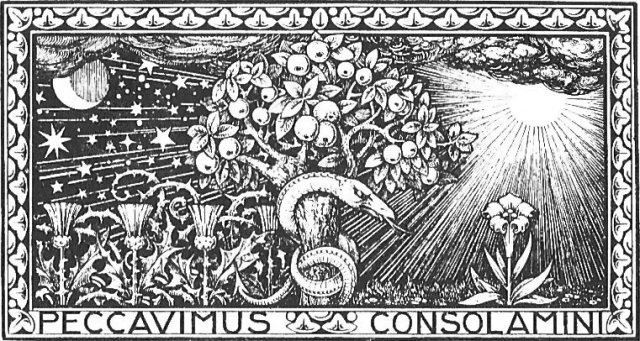
\includegraphics[width=1\textwidth,height=1\textheight,keepaspectratio]{media/pecado}
\end{nscenter}

\subsection{Preparação}

\emph{Quem quiser receber dignamente este Sacramento, diligenciará conhecer todos e cada um dos seus pecados. Assim, pois, interiormente, na presença de Deus, dirá:}

\blettrine{D}{eus} de bondade e de misericórdia, que estais sempre benignamente disposto a acolher os pecadores e a perdoar-lhes, dignai-Vos receber e atender a esta pobre alma que deseja lavar as suas nódoas nas águas salutares do sacramento da Penitência. Concedei-me a graça, ó meu Deus, de me aproximar de Vós com as necessárias disposições: iluminai o meu espírito, para que conheça todos meus pecados; tocai no meu coração,
para que os deteste sincera e firmemente; abri-me a minha boca, para que confesse integralmente; e fortificai-me a vontade, para que me emende salutarmente. Assim, ó meu Deus, e só assim, poderei alcançar o vosso perdão, tão necessário e tão desejado.

\subsubsection{Exame de Consciência}

\rlettrine{D}{ivino} Espírito Santo, concedei-me a graça de conhecer todos meus pecados tão distintamente como os conhecerei quando, ao terminar os dias nesta vida, tiver de comparecer diante de Vós, para ser julgado. Mostrai-me, não só o mal que cometi, mas ainda o bem que omiti. Iluminai-me, fortalecei-me e não permitais que a complacência criminosa, que tenho para comigo, me seduza e cegue até ao ponto de não conhecer as minhas misérias. Não me desampareis neste momento, Senhor; antes, dizei uma só palavra, e terei encontrado o remédio da salvação eterna.

\subsection{Depois do exame de consciência}

\subsubsection{Acto de dor}

\qlettrine{Q}{ue} confusão a minha, ó meu Deus, ao reconhecer que caí tantas vezes e tão facilmente nos mesmos pecados, e depois de Vos haver prometido emendar-me!... Como tenho tido coragem, ó meu Deus, de cair tantas vezes no pecado, abusando dos benefícios que me concedestes e, demais, conhecendo tão bem quanto o pecado Vos desagrada!... Ó meu Deus e meu Senhor, ó Pai eterno, aplacai a vossa justa ira e me não castigueis segundo o rigor da vossa justiça, que tanto mereço. Deixai-Vos aplacar pelos protestos de arrependimento que faço com o coração verdadeiramente contrito, ainda mais por conhecer que estes pecados Vos ofendem e desagradam, do que por saber que eles incorri nos castigos das penas eternas. Oh! sim, meu bom Jesus, tenho viva dor de Vos haver ofendido, sendo Vós tão amável, tão misericordioso!...\par
Perdão, Senhor, por todo o mal que cometi; perdão por todo o bem que omiti; perdão por todos meus pecados! Quereria reparar essas minhas ingratidões com meu sangue, com a minha própria vida. Oh! Senhor, se eu fora capaz de reparar as minhas faltas com meu arrependimento!... Supri esta minha deficiência com os merecimentos da vossa Agonia no horto; orvalhai o meu coração com uma gota desse mar de amargura em que o vosso foi, então, abismado; e que, renovado com vossa graça, me sinta penetrado de dor e tristeza mortais!

\subsubsection{Acto de bom Propósito}

\slettrine{Ó}{} meu Deus, eu não deveria viver senão para Vos amar; mas, visto que tenho tido a infelicidade de pecar, faço o propósito bem firme, auxiliado com vossa graça, de nunca mais pecar, vigiando continuamente para evitar o pecado e as suas ocasiões, e particularmente daqueles em que por fraqueza ou malícia tenho o hábito de cair. Quero sinceramente empregar todos os meios que o vosso Ministro me indicar para evitar estas quedas, cumprindo-os, como se fosseis Vós mesmo que mos indicásseis. Auxiliai-me, pois, com um pouco dessa vontade que tiveste quando Vos resolvestes a aceitar a morte na Cruz, para a salvação da humanidade.

\subsubsection{Acto de Esperança}

\rlettrine{S}{ei,} ó Deus, até que ponto Vos tenho ofendido, e o que devia esperar da vossa indignação, se não se interpusesse a vossa misericórdia, e os méritos do meu Salvador não aplacassem a vossa justiça e não solicitassem o meu perdão. Ó meu Deus, não recuseis os pedidos que o vosso amabilíssimo Filhos Vos dirige por este pecador, e perdoai-me, assim como perdoaste a tantos miseráveis que a Vós recorreram. É com esta esperança que vou comparecer diante do Sagrado Tribunal para me acusar humilde, sincera e inteiramente de todos meus pecados ao vosso Ministro, para de sua boca alcançar em vosso nome misericórdia e perdão.

\subsubsection{À B. V. Maria e Anjo da Guarda}
\slettrine{Ó}{} Virgem Santíssima, Mãe de graça e de misericórdia, e refúgio seguro dos pecadores, intercedei neste momento por mim, afim de que a Confissão, que vou fazer, não me torne ainda mais culpável, mas que me alcance perdão de todo o passado e graças necessárias para nunca mais pecar. - Meu bom Anjo, fiel e zeloso guarda da minha alma, que tendes sido testemunha das minhas quedas, consegui que este Sacramento me sirva de remédio para nunca mais cair no pecado. Amen.

\subsubsection{Acto de contrição}

\rlettrine{M}{eu} Deus, porque sois infinitamente bom e Vos amo de todo meu coração, pesa-me de Vos ter ofendido; e com o auxílio da vossa divina graça proponho firmemente emendar-me e nunca mais Vos tornar a ofender; peço e espero o perdão das minhas culpas pela vossa infinita misericórdia. Amen.

\subsection{Depois da Confissão}

\begin{nscenter}
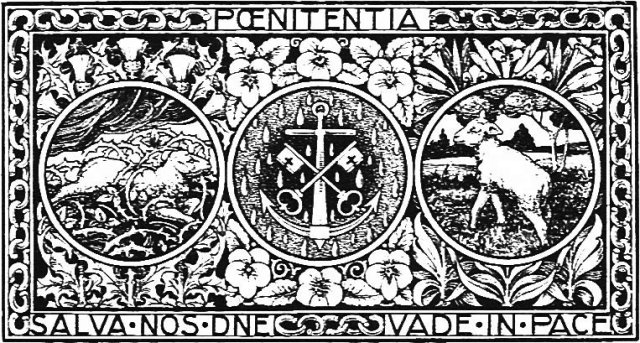
\includegraphics[width=0.8\textwidth,height=0.8\textheight,keepaspectratio]{media/penitencia}
\end{nscenter}

\subsubsection{Acto de Fé na Absolvição}

\rlettrine{O}{usarei} persuadir-me, ó meu Deus, que, de pecador que era, me encontro, presentemente, pela graça da Absolvição sacramental, perdoado e lavado das manchas das minhas culpas?! Sim, ó meu Deus de bondade, acabo de ser absolvido; e esta sentença de misericórdia restituí-me a vossa amizade, se a recebi com as devidas disposições. É ao vosso preciosíssimo Sangue, ó amável Redentor, que devo a particularíssima graça da minha reconciliação convosco, o que me dá a esperança da eterna salvação.

\subsubsection{Acção de Graças}

\slettrine{Ó}{} minha alma, agradece rendidamente ao Senhor os pródigos da sua misericórdia! É preciso, ó meu Deus, que sejais cheio de infinita indulgência para usardes de tanta liberalidade para com esta pobre criatura!... Como sois bom, ó Senhor, ó Deus, ó Pai!... Mais uma vez tenho esta consoladora experiência! Porém, como poderei testemunhar-Vos o meu reconhecimento? O menos que devo, ó Divino Redentor, é oferecer-Vos hoje e todos os dias da minha vida um sacrifício perene de louvores; engrandecer incessantemente a vossa infinita misericórdia. Eu o faço de todo o coração, ó meu Deus, e o farei até à morte. Sim, durante toda minha vida, louvarei, honrarei, amarei e glorificarei o Senhor, que é tão terno amante da minha pobre alma e quer levá-la consigo aos gozos da glória incomparável da vida eterna!...

\subsubsection{Propósito de nunca Mais pecar}

\slettrine{Ó}{} meu Deus, o benefício que acabais de praticar em meu favor inspira-me tal ódio ao pecado, que me obriga a tomar sinceramente a resolução de nunca mais pecar. Vos prometo, ó meu Deus, que hei-de esforçar-me tanto quanto possa para mudar de vida. Fortificai, ó Senhor, esta minha resolução; tornai eficaz o propósito que faço de evitar todas as ocasiões de pecado, principalmente daquele que mais Vos desagrada e em que tenho caído tantas vezes e desde há tanto tempo! Empregarei todos os meios para o evitar; eu me obrigarei até por meios violentos a conseguir este meu propósito. Ó Maria, minha boa e terna Mãe, amparo dos mortais, auxílio dos cristãos e refúgio dos pecadores, a Vós recomendo esta resolução, esperando que me auxiliareis a cumpri-la. Amen.

%%%%%%%%%%%%%%%%%%%%ROSÁRIO%%%%%%%%%%%%%%%%%%%%
\newpage\section{Rosário}

\subsection{Sinal da Cruz}
\begin{paracol}{2}\latim{
\cruz In nómine Patris, et Fílii, et Spíritus Sancti. Amen.
}\switchcolumn\portugues{
\cruz Em nome do Pai e do Filho e do Espírito Santo. Amen.
}\end{paracol}


\subsectioninfo{Símbolo dos Apóstolos}{Página \pageref{simboloapostolos}}

\subsubsection{Oferecimento do Santo Rosário}

\rlettrine{S}{antíssima} Virgem, Mãe de Deus, eu Vos ofereço este rosário em desagravo do Santíssimo Coração de Nosso Senhor Jesus Cristo, vosso Filho, e em desagravo do vosso Coração Imaculado; e pelas intenções que Vos apresento: \emph{(Referir as intenções.)}

\subsubsection{Intenções do Santo Padre}
\begin{compactitem}
\begin{paracol}{2}\latim{
\item Exaltatio S. Matris Ecclesiæ.
}\switchcolumn\portugues{
\item Exaltação da Santa Igreja.
}\switchcolumn*\latim{
\item Propagatio fidei.
}\switchcolumn\portugues{
\item Propagação da fé.
}\switchcolumn*\latim{
\item Extirpatio hæresum.
}\switchcolumn\portugues{
\item Extirpação das heresias.
}\switchcolumn*\latim{
\item Conversio peccatorum.
}\switchcolumn\portugues{
\item Conversão dos pecadores.
}\switchcolumn*\latim{
\item Pax inter principes christianos.
}\switchcolumn\portugues{
\item Paz entre os Reis e Príncipes católicos.
}\end{paracol}
\end{compactitem}

\subsection{Pedras Maiores}
\subsubsection{Pai Nosso}
\begin{paracol}{2}\latim{
℣. Pater noster, qui es in cælis: sanctificétur nomen tuum: advéniat regnum tuum: fiat volúntas tua, sicut in cælo, et in terra.
}\switchcolumn\portugues{
℣. Pai Nosso, que estais nos céus, santificado seja o vosso Nome, venha a nós o vosso Reino; seja feita a vossa vontade assim na terra como no Céu.
}\switchcolumn*\latim{
℟. Panem nostrum quotidiánum da nobis hódie: et dimítte nobis débita nostra, sicut et nos dimíttimus debitóribus nostris. Et ne nos indúcas in tentatiónem. Sed líbera nos a malo. Amen.
}\switchcolumn\portugues{
℟. O pão nosso de cada dia nos dai hoje; perdoai-nos as nossas ofensas, assim como nós perdoamos a quem nos tem ofendido; e não nos deixeis cair em tentação; mas livrai-nos do mal. Amen.
}\end{paracol}


\subsection{Pedras Menores}
\subsubsection{Ave Maria}
\begin{paracol}{2}\latim{
℣. Ave, María, grátia plena, Dóminus tecum; benedícta tu in muliéribus, et benedíctus fructus ventris tui, Jesus.
}\switchcolumn\portugues{
℣. Ave, Maria, Cheia de graça, o Senhor é convosco; bendita sois Vós entre as mulheres, e bendito é o fruto do vosso ventre, Jesus.
}\switchcolumn*\latim{
℟. Sancta María, Mater Dei, ora pro nobis peccatóribus, nunc, et in hora mortis nostræ. Amen.
}\switchcolumn\portugues{
℟. Santa Maria, Mãe de Deus, rogai por nós, pecadores, agora e na hora da nossa morte. Amen.
}\end{paracol}


\subsection{Fim da Dezena}
\subsubsection{Glória}
\begin{paracol}{2}\latim{
℣. Glória Patri, et Fílio, et Spíritui Sancto.
}\switchcolumn\portugues{
℣. Glória ao Pai, e ao Filho e ao Espírito Santo.
}\switchcolumn*\latim{
℟. Sicut erat in pricípio, et nunc, et semper, et in sǽcula sæculórum. Amen.
}\switchcolumn\portugues{
℟. Assim como era no princípio, agora e sempre, e por todos os séculos dos séculos. Amen.
}\end{paracol}


\subsubsection{Nossa Senhora a Santa Catarina Labouré}\label{concebidasempecado}
\begin{paracol}{2}\latim{
℣. O Maria sine labe concepta.
}\switchcolumn\portugues{
℣. Ó Maria concebida sem pecado.
}\switchcolumn*\latim{
℟. Ora pro nobis, qui confugimus ad te.
}\switchcolumn\portugues{
℟. Rogai por nós que recorremos a vós.
}\end{paracol}

\subsubsection{Nossa Senhora aos Santos Pastorinhos}
\begin{paracol}{2}\latim{
℣. Oh mi Jesu, dimitte nobis débita nostra, líbera nos ab igne inférni,
}\switchcolumn\portugues{
℣. Ó meu Jesus, perdoai-nos e livrai-nos do fogo do inferno,
}\switchcolumn*\latim{
℟. Conduc in cælum omnes animas, præsértim illas quæ máxime indigent misericórdia tua.
}\switchcolumn\portugues{
℟. Levai as alminhas todas para o Céu e socorrei principalmente as que mais precisarem.
}\end{paracol}


\subsection{Meditações do Rosário}

\subsubsection{Mystérios Gozosos}
\begin{nscenter}\emph{Segunda-feira e Quinta-feira}\end{nscenter}

{\redx Primeiro Mystério:} Meditemos na Anunciação do Arcanjo São Gabriel à Santíssima Virgem, e roguemos a virtude da humildade.\par
{\redx Segundo Mystério:} Meditemos na Visitação da Santíssima Virgem a sua Prima, Santa Isabel, e roguemos a caridade para com o próximo.\par
{\redx Terceiro Mystério:} Meditemos no Nascimento do Menino Jesus, e roguemos o desprendimento dos bens do mundo.\par
{\redx Quarto Mystério:} Meditemos na Apresentação do Menino Jesus no Templo e na Purificação de Nossa Senhora, e roguemos a obediência e a pureza do espírito e do coração.\par
{\redx Quinto Mystério:} Meditemos na Perda e no Encontro do Menino Jesus no Templo, e roguemos o conhecimento das cousas divinas e a prontidão no serviço de Deus.

\subsubsection{Mystérios Dolorosos}
\begin{nscenter}\emph{Terça-feira e Sexta-feira}\end{nscenter}

{\redx Primeiro Mystério:} Meditemos na Agonia de N. S. Jesus Cristo, e roguemos a contrição dos nossos pecados.\par
{\redx Segundo Mystério:} Meditemos na flagelação de N. S. Jesus Cristo, e roguemos a mortificação dos sentidos.\par
{\redx Terceiro Mystério:} Meditemos na Coroação de Espinhos de N. S. Jesus Cristo, e roguemos a mortificação do espírito e do coração.\par
{\redx Quarto Mystério:} Meditemos em N. S. Jesus Cristo levando a Cruz para o Calvário, e roguemos a paciência e a resignação.\par
{\redx Quinto Mystério:} Meditemos na Crucifixão e Morte de N. S. Jesus Cristo, e roguemos o amor a Deus e a salvação das almas.

\subsubsection{Mystérios Gloriosos}
\begin{nscenter}\emph{Quarta-feira, Sábado e Domingo}\end{nscenter}

{\redx Primeiro Mystério:} Meditemos na Ressurreição de N. S. Jesus Cristo, e roguemos para recebermos o dom da fé e para a conversão dos pecadores.\par
{\redx Segundo Mystério:} Meditemos na Ascensão de N. S. Jesus Cristo, e roguemos a esperança e o desejo do céu.\par
{\redx Terceiro Mystério:} Meditemos na descida do Divino Espírito Santo, e roguemos o amor a Deus e o zelo da salvação das almas.\par
{\redx Quarto Mystério:} Meditemos na Assunção da Santíssima Virgem, e roguemos a graça de uma boa morte e a devoção a Nossa Senhora.\par
{\redx Quinto Mystério:} Meditemos na Coroação da Santíssima Virgem, e roguemos a perseverança final e a confiança em Nossa Senhora.

\subsection{Fim do Rosário}

\emph{Procurar Antifona de Nossa Senhora própria do Tempo na página \pageref{antifonasnossasenhora} ou rezar a Salve Regina.}

\subsubsectioninfo{Salve Regina}{Página \pageref{salveregina}}

\subsubsectioninfo{Ladainha de Nossa Senhora}{Página \pageref{ladainhaloreto}}

%%%%%%%%%%%%%%%%%%%%VIA SACRA%%%%%%%%%%%%%%%%%%%%
\newpage\section{Via Sacra}

\paragraph{No início:}

\blettrine{M}{eu} Senhor e meu Deus, sob o olhar amoroso de Nossa Mãe, dispomo-nos a acompanhar-Vos pelo caminho de dor que foi o preço do nosso resgate.
Queremos sofrer tudo o que Vós sofrestes, oferecer-Vos o nosso pobre coração, contrito, porque sois inocente e vais sofrer por nós, que somos os únicos culpados.

\blettrine{M}{inha} Mãe, Virgem dolorosa, ajudai-me a reviver aquelas horas amargas que o vosso Filho quis passar na terra, para que nós, feitos de um punhado de lodo, vivêssemos por fim \emph{in libertatem gloriæ filiorum Dei} (na liberdade e glória dos filhos de Deus.).

\paragraph{Depois de enunciar cada Estação:}

\begin{paracol}{2}\latim{
℣. Adorámus te, Christe, et benedicimus tibi.
}\switchcolumn\portugues{
℣. Nós Vos adoramos, ó Jesus, e Vos bendizemos.
}\switchcolumn*\latim{
℟. Quia per Crucem tuam redemísti mundum.
}\switchcolumn\portugues{
℟. Porque pela vossa Santa Cruz redimistes o mundo.
}\end{paracol}

\paragraph{No fim de cada Estação:}
\emph{Pai nosso, Ave Maria, Glória.}
\begin{paracol}{2}\latim{
℣. Miserére nostri, Dómine.
}\switchcolumn\portugues{
℣. Senhor tende piedade de nós.
}\switchcolumn*\latim{
℟. Miserére nostri.
}\switchcolumn\portugues{
℟. Tende piedade de nós.
}\end{paracol}

\newpage

\paragraph{Estação 1}

\begin{nscenter}
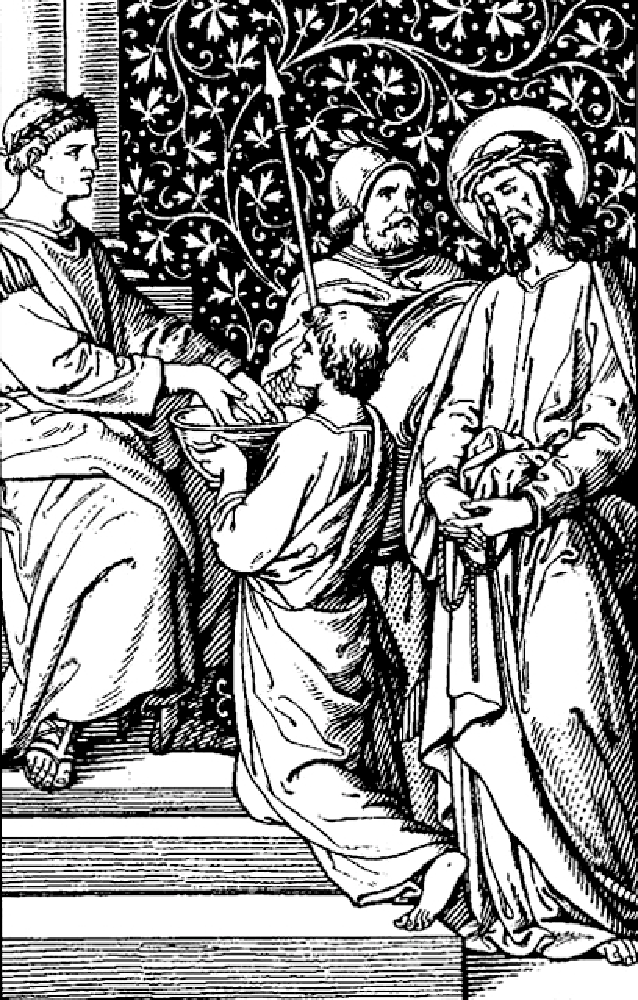
\includegraphics[width=.8\textwidth, height=.8\textheight, keepaspectratio]{media/station1}
\end{nscenter}

\blettrine{N}{esta} primeira estação contemplemos N. S. J. C., que, depois de cruelmente açoitado e coroado de espinhos, é levado pela segunda vez à presença de Pilatos, que por instigação dos judeus O condena à morte.
E Jesus, que quere padecer e morrer para nos provar o seu amor e livrar-nos do Inferno, submete-se à condenação!...
Ó misericordiosíssimo Jesus, fazei-nos compreender o vosso amor, e abrasai-nos nele.

\pagebreak

\paragraph{Estação 2}

\begin{nscenter}
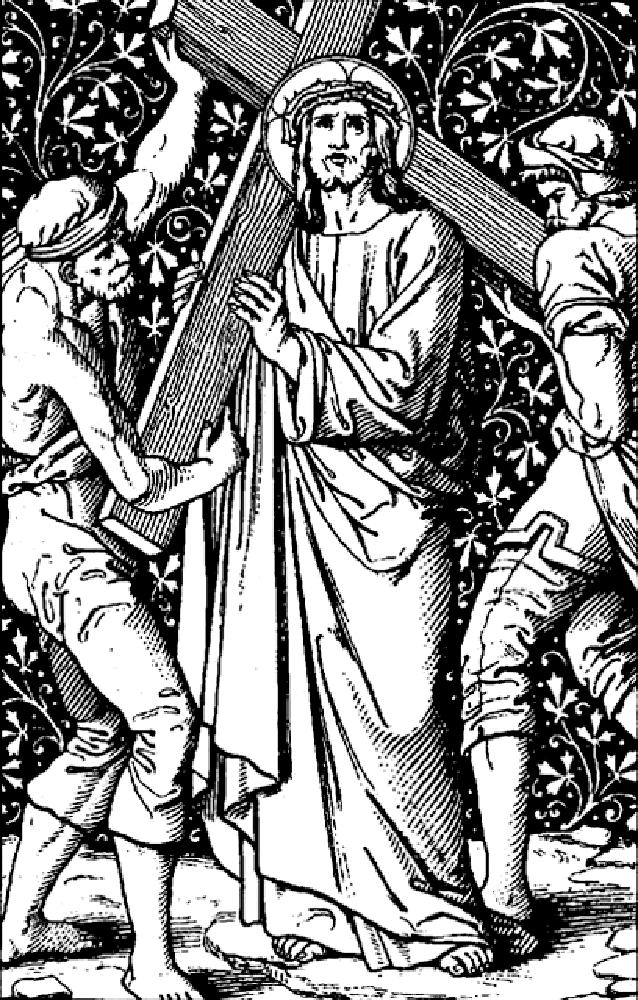
\includegraphics[width=.8\textwidth, height=.8\textheight, keepaspectratio]{media/station2}
\end{nscenter}

\blettrine{N}{esta} segunda estação contemplemos N. S. J. C., tratado com desprezo pelos algozes, que O obrigam a levar às costas, sobre as chagas vivas dos açoites, a pesadíssima Cruz em que vai ser crucificado para nos salvar!
Ó misericordiosíssimo Jesus, ajudai-nos a sofrer generosamente por vosso amor os desprezos e humilhações de cada dia.

\newpage

\paragraph{Estação 3}

\begin{nscenter}
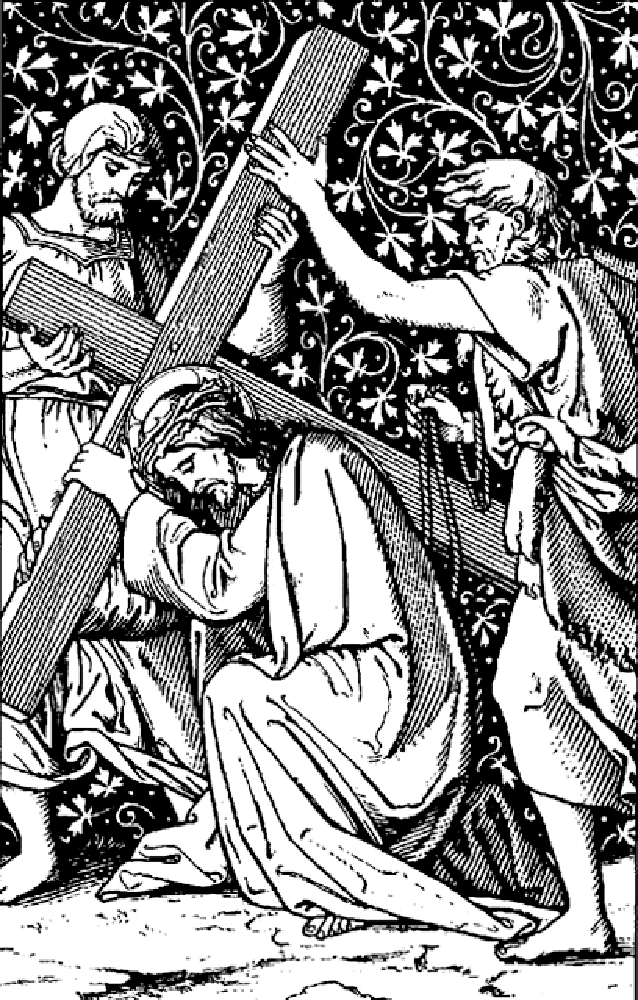
\includegraphics[width=.8\textwidth, height=.8\textheight, keepaspectratio]{media/station3}
\end{nscenter}

\blettrine{N}{esta} terceira estação contemplemos N. S. J. C., arrastado e empurrado pelos algozes! Então cai sob o peso da Cruz e fere os joelhos nas pedras do caminho!...
Ó misericordiosíssimo Jesus, pelas vossas chagas, concedei-nos a graça de detestar o pecado para melhor correspondermos ao vosso amor.

\newpage

\paragraph{Estação 4}

\begin{nscenter}
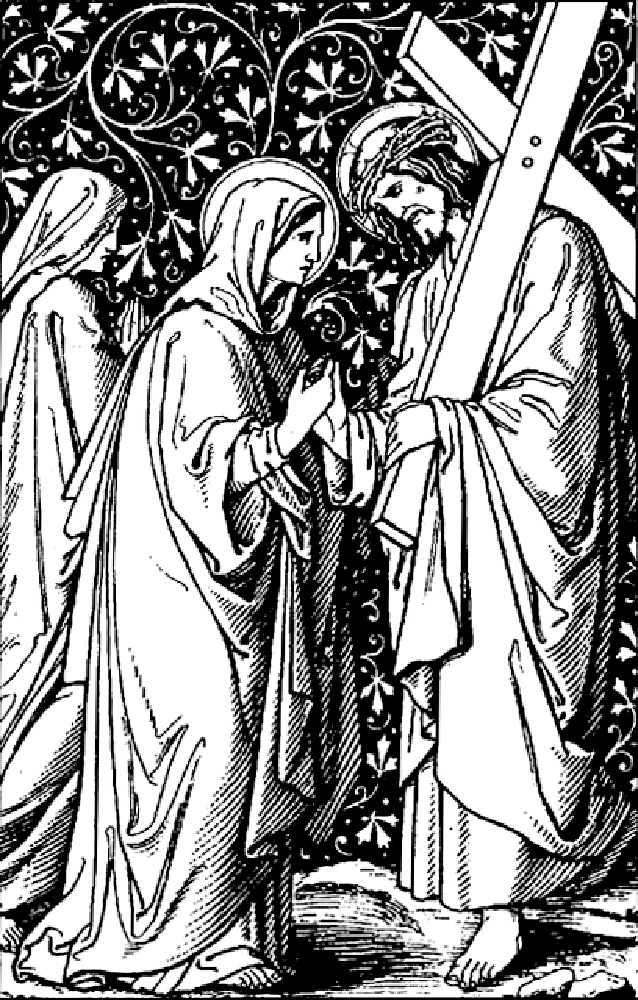
\includegraphics[width=.8\textwidth, height=.8\textheight, keepaspectratio]{media/station4}
\end{nscenter}

\blettrine{N}{esta} quarta estação contemplemos N. S. J. C., rodeado de seus inimigos e todo pisado e ensanguentado. Encontra sua Mãe, que num impulso de amor e dor corre pare Ele através da multidão, que cruelmente O escarnece e se regozija com o sofrimento daquela terna Mãe e do seu carinhoso Filho!...
Jesus e Maria, assisti-nos na última agonia.

\newpage

\paragraph{Estação 5}

\begin{nscenter}
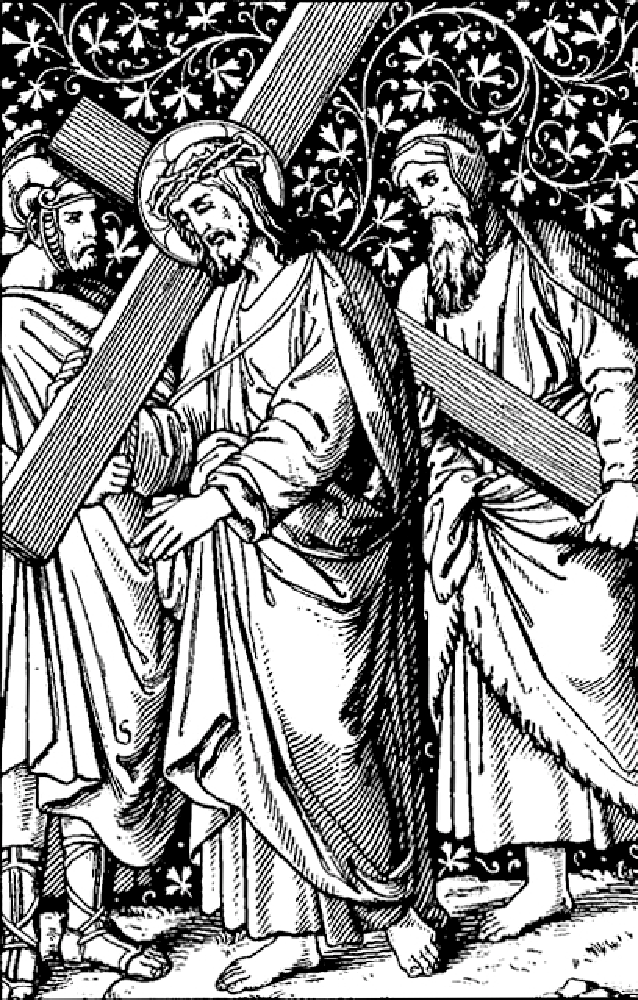
\includegraphics[width=.8\textwidth, height=.8\textheight, keepaspectratio]{media/station5}
\end{nscenter}

\blettrine{N}{esta} quinta estação contemplemos N. S. J. C., vergado sob o peso da Cruz e atormentado com as dores da grande chaga que ela abriu emseu ombro. Mal se mexe; já não pode caminhar; e os algozes, temendo que morra antes de ser crucificado, intimam Simão Cireneu a que O ajude!...
Ó misericordiosíssimo Jesus, ajudai-nos a levar a cruz, que for da vossa vontade enviar-nos.

\newpage

\paragraph{Estação 6}

\begin{nscenter}
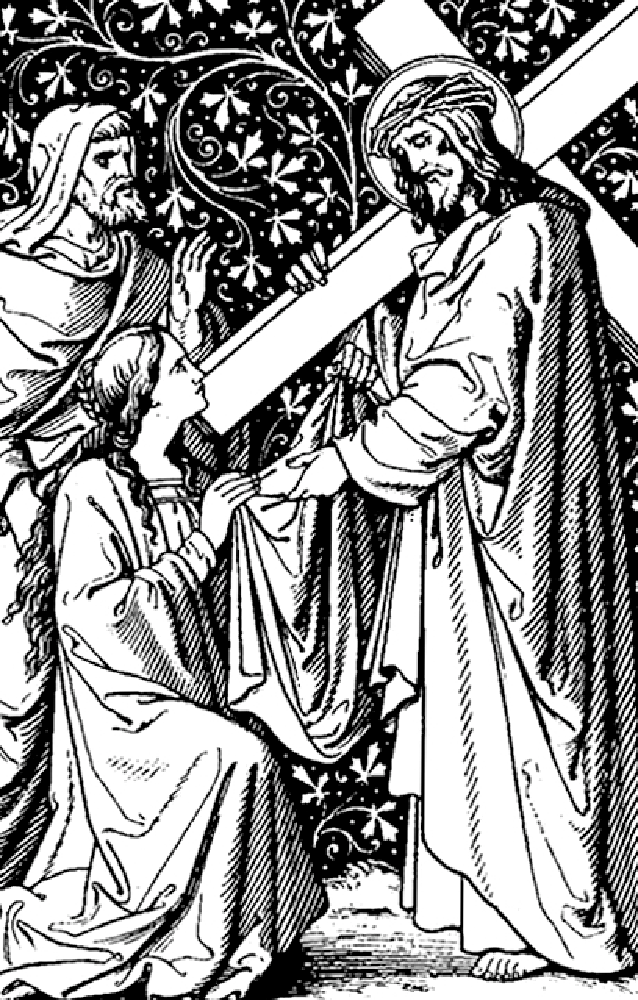
\includegraphics[width=.8\textwidth, height=.8\textheight, keepaspectratio]{media/station6}
\end{nscenter}

\blettrine{N}{esta} sexta estação contemplemos N. S. J. C., que deixa seu retracto estampando no véu que uma caridosa mulher Lhe ofereceu, para limpar o rosto do suor e sangue que Lhe toldavam a vista!...
Ó misericordiosíssimo Jesus, imprimi na nossa alma a vossa imagem, desfigurada pelos tormentos, para que nunca esqueçamos o que sofrestes por amor de nós.

\newpage

\paragraph{Estação 7}

\begin{nscenter}
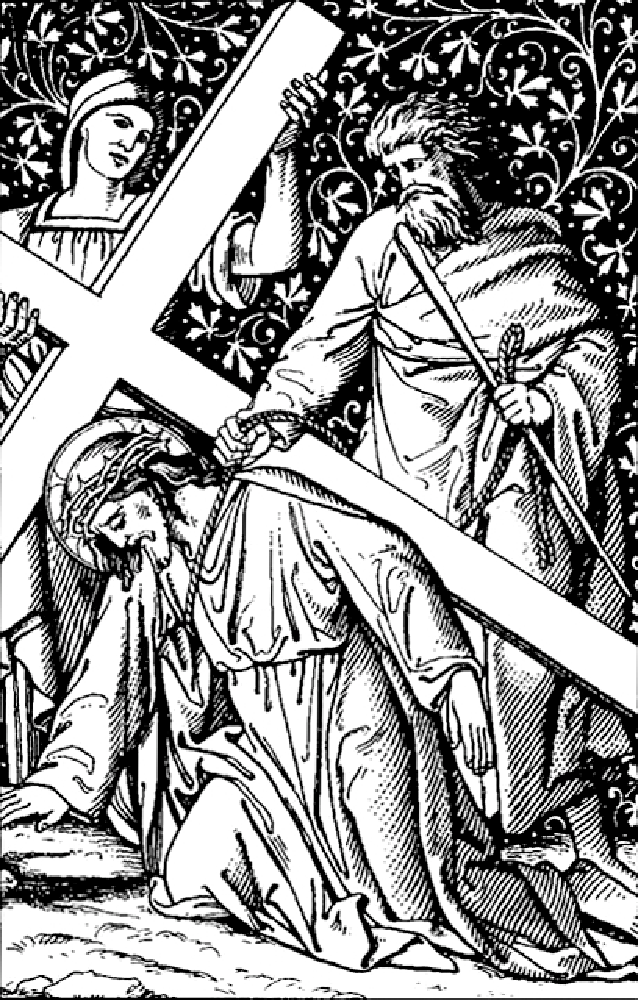
\includegraphics[width=.8\textwidth, height=.8\textheight, keepaspectratio]{media/station7}
\end{nscenter}

\blettrine{N}{esta} sétima estação contemplemos N. S. J. C., exausto de forças, desfalecido e caído por terra, atordoado pela algazarra infernal da plebe, que O insulta e Lhe escarra no rosto. Os algozes, impacientes por chegarem ao Calvário, violentamente O levantam, descarregando-lhe murros e pontapés!...
Ó misericordiosíssimo Jesus, nos não deixes desfalecer no vosso serviço. Conformai-nos em tudo com vossa santíssima vontade.

\newpage

\paragraph{Estação 8}

\begin{nscenter}
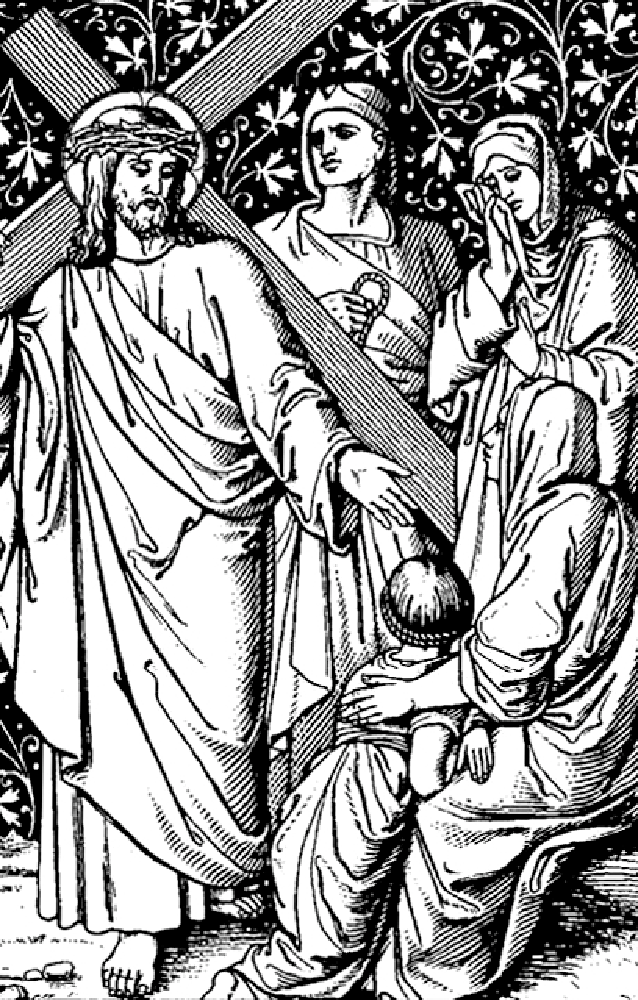
\includegraphics[width=.8\textwidth, height=.8\textheight, keepaspectratio]{media/station8}
\end{nscenter}

\blettrine{N}{esta} oitava estação contemplemos N. S. J. C., que esquece as suas dores para se compadecer das piedosas mulheres, que por Ele choram, e lhes diz: Filhas de Jerusalém, não choreis sobre Mim; chorai sobre vós mesmas e sobre vosso filhos!...
Ó misericordiosíssimo Jesus, dai-nos lágrimas de sincero arrependimento, para chorar os nossos pecados, causa dos vossos tormentos.

\newpage

\paragraph{Estação 9}

\begin{nscenter}
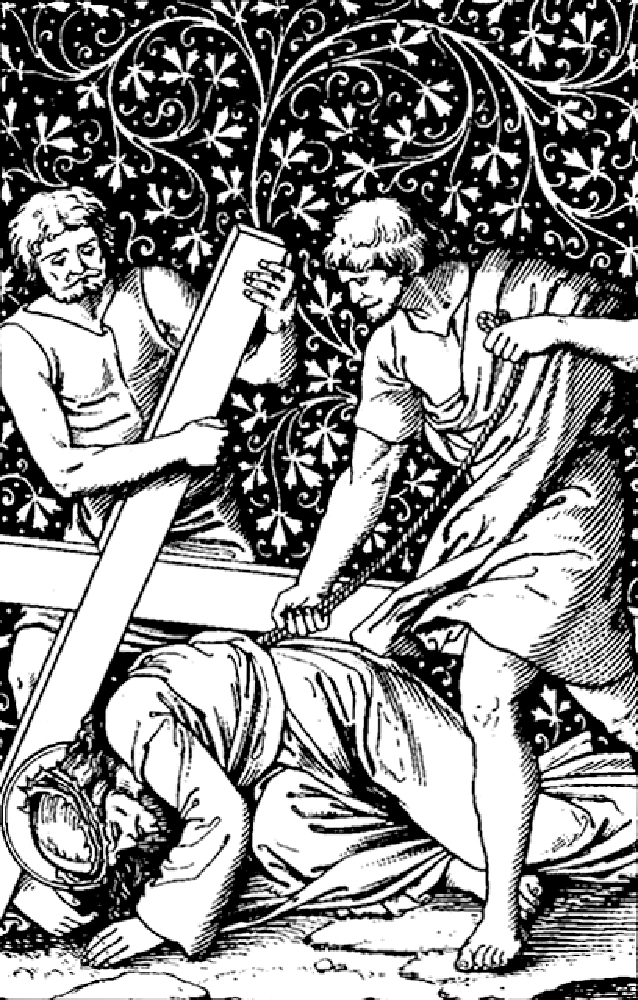
\includegraphics[width=.8\textwidth, height=.8\textheight, keepaspectratio]{media/station9}
\end{nscenter}

\blettrine{N}{esta} nona estação contemplemos N. S. J. C., que chega ao Calvários, banhado em sangue, e mais morto que vivo; e, não podendo aguentar de pé os empurrões e pancadas que Lhe dão os algozes, cai desamparado e chegar a tocar a terra com sua santíssima boca!...
Ó misericordiosíssimo Jesus, pelas vossas chagas Vos pedimos que tenhais compaixão dos que caíram em pecado e nele vivem; salvai-nos!

\newpage

\paragraph{Estação 10}

\begin{nscenter}
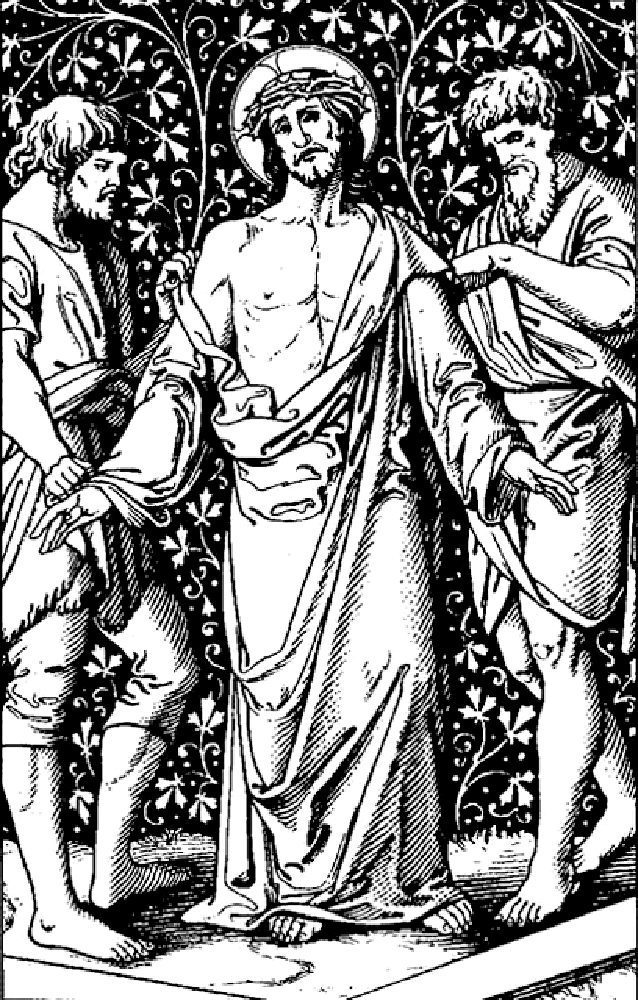
\includegraphics[width=.8\textwidth, height=.8\textheight, keepaspectratio]{media/station10}
\end{nscenter}

\blettrine{N}{esta} décima estação contemplemos N. S. J. C., cruelmente despojado de seus vestidos, que estavam colados às feridas, as quais novamente sangram, fazendo-o tremer com dores!...
Ó misericordiosíssimo Jesus, despojai-nos do orgulho, da vaidade e dos respeitos humanos com que tanto Vos temos ofendido e atraiçoado.

\newpage

\paragraph{Estação 11}

\begin{nscenter}
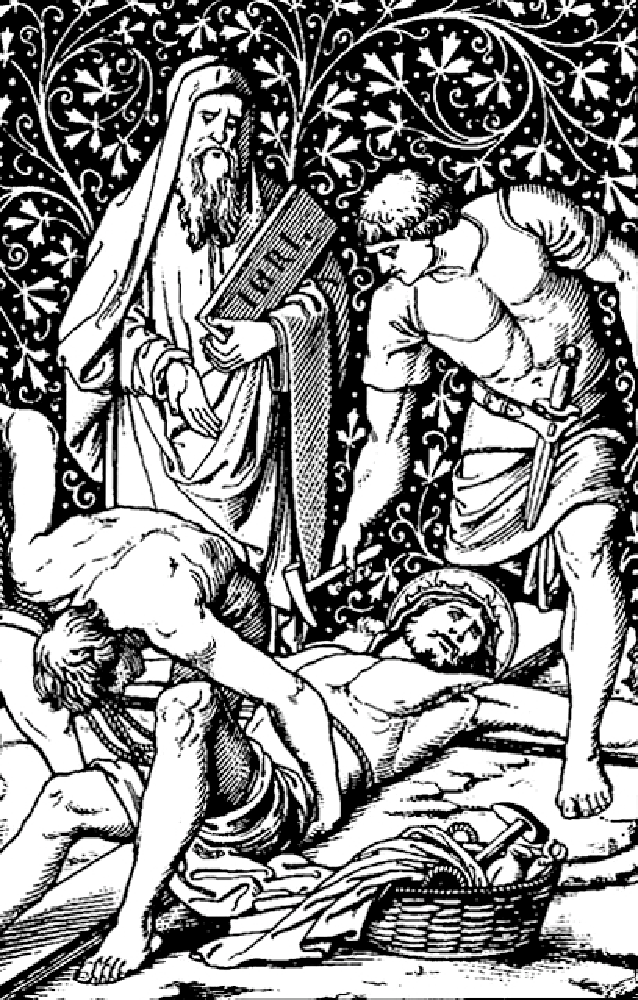
\includegraphics[width=.8\textwidth, height=.8\textheight, keepaspectratio]{media/station11}
\end{nscenter}

\blettrine{N}{esta} décima primeira estação contemplemos N. S. J. C., pregado na Cruz tão barbaramente que Lhe deslocam os ossos. Maria Santíssima, com o coração despedaçado de dor, ouve as pancadas do martelo que enterram os cravos nas mãos e pés doseu amado Filho, Lhe não podendo valer!...
Ó Santa Mãe das dores, gravai em meu coração as chagas do Salvador.

\newpage

\paragraph{Estação 12}

\begin{nscenter}
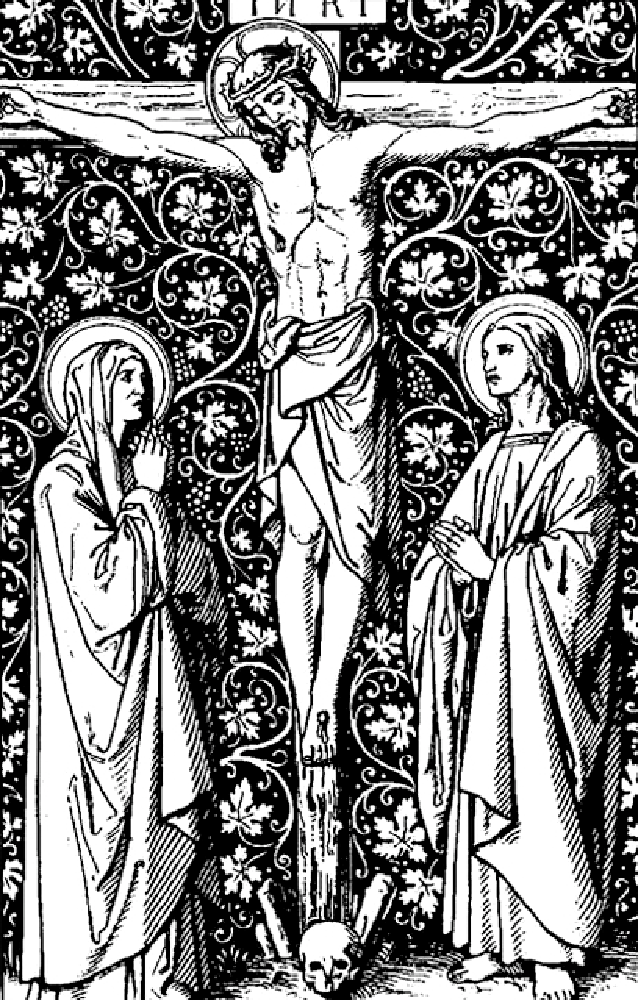
\includegraphics[width=.8\textwidth, height=.8\textheight, keepaspectratio]{media/station12}
\end{nscenter}

\blettrine{N}{esta} décima segunda estação contemplemos N. S. J. C., levantado na Cruz e exposto entre dous ladrões ao escárnio e insultos da plebe, até exalar o último suspiro!...
Ó clementíssimo Jesus, que Vos abrasais em ardente amor pelas almas, eu Vos suplico pela agonia do vosso Santíssimo coração e pelas dores de vossa Mãe Imaculada, que purifiqueis no vosso Sangue todos os pecadores do mundo que neste momento estão em agonia e hoje hão-de morrer.

\newpage

\paragraph{Estação 13}

\begin{nscenter}
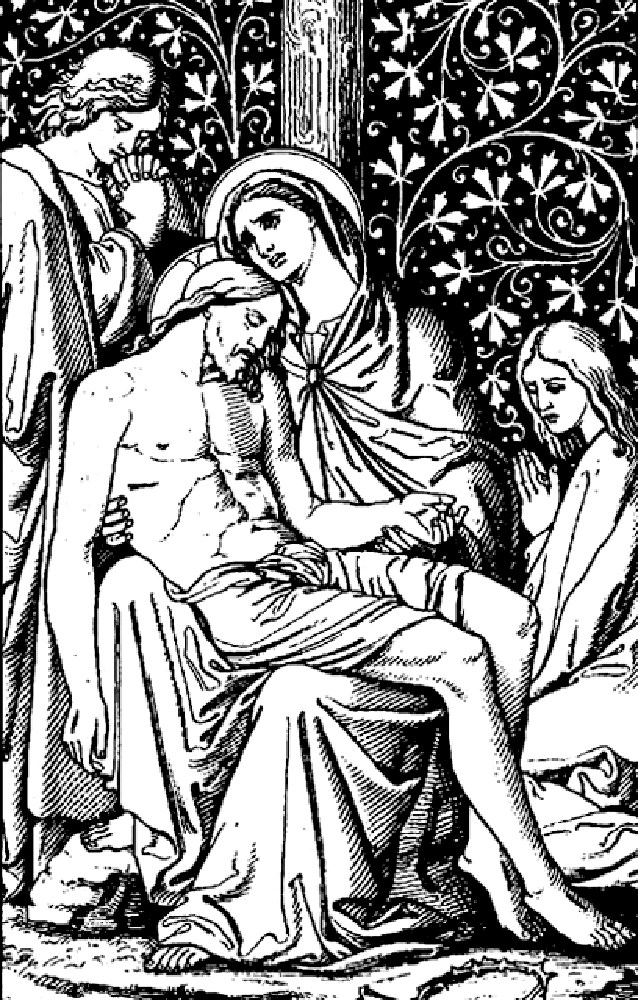
\includegraphics[width=.75\textwidth, height=.75\textheight, keepaspectratio]{media/station13}
\end{nscenter}

\blettrine{N}{esta} décima terceira estação contemplemos N. S. J. C., despregado piedosamente da Cruz pelos seus amigos e depositado no regaço de sua Mãe, que, banhada em lágrimas, beija e abraça o corpo deseu Filho, denegrido com pancadas e coberto de feridas, e algumas tão profundas que deixam ver os seus ossos!...
Ó Santa Mãe das dores, rogai a Jesus que nos perdoe os pecados, nos ajude a imitar as vossas virtudes, nos conceda a graça da perseverança final e nos purifique com seu precioso Sangue, para podermos satisfazer à sua justiça e gozá-lo no Céu por toda a eternidade. Ó Jesus, por amor de Maria nossa mãe, concedei-nos esta graça.

\newpage

\paragraph{Estação 14}

\begin{nscenter}
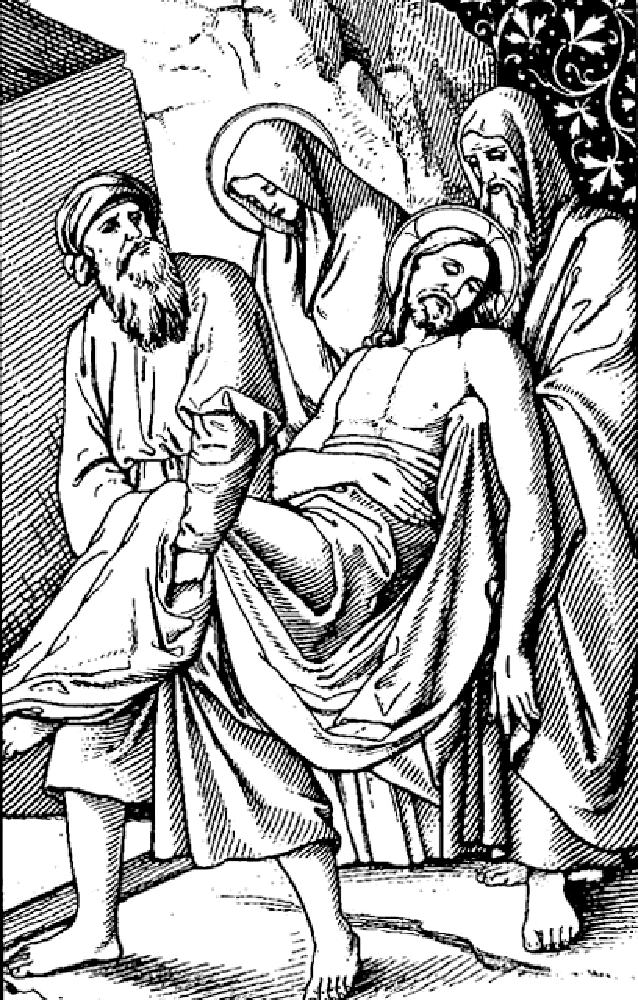
\includegraphics[width=.8\textwidth, height=.8\textheight, keepaspectratio]{media/station14}
\end{nscenter}

\blettrine{N}{esta} décima quarta estação contemplemos N. S. J. C. no sepulcro, e Maria Santíssima mais que nunca angustiada em triste saudade!...
Ó Mãe, fonte de amor, fazei que eu sinta as vossas fortes dores e convosco chore.
Pai eterno, misericórdia, pelo precioso sangue de Jesus.

\newpage

\paragraph{Oração final}

\emph{Depois desta Estação, reza-se o Pai nosso... a Ave Maria... e a Glória ao Pai... cinco vezes, em honra das cinco chagas de nosso Senhor Jesus Cristo. Mais um Pai nosso, uma Ave Maria e uma Glória ao Pai pelas intenções do Santo Padre, terminando-se com a seguinte oração:}

\paragraph{Commendatio}

\begin{paracol}{2}\latim{
\blettrine{R}{espice,} quǽsumus Dómine, super hanc famíliam tuam, pro qua Dominus noster Jesus Christus non dubitavit manibus tradi nocentium et Crucis subire
tormentum. Qui tecum vivit et regnat in unitate Spíritus Sancti, Deus, per ómnia sǽcula sæculórum.
}\switchcolumn\portugues{
\blettrine{S}{enhor,} dignai-Vos lançar um olhar sobre a vossa família pela qual nosso Senhor Jesus Cristo não duvidou entregar-se às mãos dos ímpios e de sofrer o suplício da cruz. Que vive e reina na unidade do Espírito Santo, Deus, por todos os séculos dos séculos.
}\switchcolumn*\latim{
℟. Amen.
}\switchcolumn\portugues{
℟. Amen.
}\end{paracol}

%%%%%%%%%%%%%%%%%%%%LADAINHAS%%%%%%%%%%%%%%%%%%%%
\newpage\section{Ladainhas}

\subsection{Ladainha do Santíssimo Nome de Jesus}\label{ladainhanomejesus}
\begin{paracol}{2}\latim{
Kyrie eleison.
}\switchcolumn\portugues{
Senhor, tende piedade de nós.
}\switchcolumn*\latim{
Christe eleison.
}\switchcolumn\portugues{
Jesus Cristo, tende piedade de nós.
}\switchcolumn*\latim{
Kyrie eleison.
}\switchcolumn\portugues{
Senhor, tende piedade de nós.
}\switchcolumn*\latim{
Jesu, audi nos.
}\switchcolumn\portugues{
Jesus Cristo, ouvi-nos.
}\switchcolumn*\latim{
Jesu, exaudi nos.
}\switchcolumn\portugues{
Jesus Cristo, atendei-nos.
}\switchcolumn*\latim{
Pater de cœlis Deus, miserere nobis.
}\switchcolumn\portugues{
Pai Celeste, que sois Deus, tende piedade de nós.
}\switchcolumn*\latim{
Fili redemptor mundi Deus,\footnote[2]{miserere nobis.\label{miserere}}
}\switchcolumn\portugues{
Filho, Redentor do mundo, que sois Deus,\footnote[2]{tende piedade de nós.\label{tende}}
}\switchcolumn*\latim{
Sancta trinitas, unus Deus,\footref{miserere}
}\switchcolumn\portugues{
Santíssima Trindade, que sois um só Deus,\footref{tende}
}\switchcolumn*\latim{
Jesu, fili dei vivi,\footref{miserere}
}\switchcolumn\portugues{
Jesus, Filho do Deus vivo,\footref{tende}
}\switchcolumn*\latim{
Jesu, candor lucis æternæ,\footref{miserere}
}\switchcolumn\portugues{
Jesus, pureza da luz eterna,\footref{tende}
}\switchcolumn*\latim{
Jesu, rex gloriæ,\footref{miserere}
}\switchcolumn\portugues{
Jesus, Rei da glória,\footref{tende}
}\switchcolumn*\latim{
Jesu, sol justitiæ,\footref{miserere}
}\switchcolumn\portugues{
Jesus, sol de justiça,\footref{tende}
}\switchcolumn*\latim{
Jesu, fili mariæ virginis,\footref{miserere}
}\switchcolumn\portugues{
Jesus, Filho da Virgem Maria,\footref{tende}
}\switchcolumn*\latim{
Jesu amabilis,\footref{miserere}
}\switchcolumn\portugues{
Jesus amável,\footref{tende}
}\switchcolumn*\latim{
Jesu admirabilis,\footref{miserere}
}\switchcolumn\portugues{
Jesus admirável,\footref{tende}
}\switchcolumn*\latim{
Jesu, Deus fortis,\footref{miserere}
}\switchcolumn\portugues{
Jesus, Deus forte,\footref{tende}
}\switchcolumn*\latim{
Jesu potentissime,\footref{miserere}
}\switchcolumn\portugues{
Jesus poderosíssimo,\footref{tende}
}\switchcolumn*\latim{
Jesu patientissime,\footref{miserere}
}\switchcolumn\portugues{
Jesus pacientíssimo,\footref{tende}
}\switchcolumn*\latim{
Jesu obedientissime,\footref{miserere}
}\switchcolumn\portugues{
Jesus obedientíssimo,\footref{tende}
}\switchcolumn*\latim{
Jesu, mitis et humilis corde,\footref{miserere}
}\switchcolumn\portugues{
Jesus, manso e humilde de coração,\footref{tende}
}\switchcolumn*\latim{
Jesu, amator castitatis,\footref{miserere}
}\switchcolumn\portugues{
Jesus, amante da castidade,\footref{tende}
}\switchcolumn*\latim{
Jesu, amator noster,\footref{miserere}
}\switchcolumn\portugues{
Jesus, nosso amado,\footref{tende}
}\switchcolumn*\latim{
Jesu, Deus pacis,\footref{miserere}
}\switchcolumn\portugues{
Jesus, Deus da paz,\footref{tende}
}\switchcolumn*\latim{
Jesu, auctor vitæ,\footref{miserere}
}\switchcolumn\portugues{
Jesus, autor da vida,\footref{tende}
}\switchcolumn*\latim{
Jesu, exemplar virtutum,\footref{miserere}
}\switchcolumn\portugues{
Jesus, exemplar das virtudes,\footref{tende}
}\switchcolumn*\latim{
Jesu, zelator animarum,\footref{miserere}
}\switchcolumn\portugues{
Jesus, zelador das almas,\footref{tende}
}\switchcolumn*\latim{
Jesu, Deus noster,\footref{miserere}
}\switchcolumn\portugues{
Jesus, nosso Deus,\footref{tende}
}\switchcolumn*\latim{
Jesu, refugium nostrum,\footref{miserere}
}\switchcolumn\portugues{
Jesus, nosso refúgio,\footref{tende}
}\switchcolumn*\latim{
Jesu, pater pauperum,\footref{miserere}
}\switchcolumn\portugues{
Jesus, Pai dos pobres,\footref{tende}
}\switchcolumn*\latim{
Jesu, thesaure fidelium,\footref{miserere}
}\switchcolumn\portugues{
Jesus, tesouro dos fiéis,\footref{tende}
}\switchcolumn*\latim{
Jesu, bone pastor,\footref{miserere}
}\switchcolumn\portugues{
Jesus, boníssimo Pastor,\footref{tende}
}\switchcolumn*\latim{
Jesu, lux vera,\footref{miserere}
}\switchcolumn\portugues{
Jesus, luz verdadeira,\footref{tende}
}\switchcolumn*\latim{
Jesu, sapientia æterna,\footref{miserere}
}\switchcolumn\portugues{
Jesus, sabedoria eterna,\footref{tende}
}\switchcolumn*\latim{
Jesu, bonitas infinita,\footref{miserere}
}\switchcolumn\portugues{
Jesus, bondade infinita,\footref{tende}
}\switchcolumn*\latim{
Jesu, via et vita nostra,\footref{miserere}
}\switchcolumn\portugues{
Jesus, caminho e vida nossa,\footref{tende}
}\switchcolumn*\latim{
Jesu, gaudium angelorum,\footref{miserere}
}\switchcolumn\portugues{
Jesus, alegria dos anjos,\footref{tende}
}\switchcolumn*\latim{
Jesu, rex patriarcharum,\footref{miserere}
}\switchcolumn\portugues{
Jesus, Rei dos patriarcas, \footref{tende}
}\switchcolumn*\latim{
Jesu, magister apostolorum,\footref{miserere}
}\switchcolumn\portugues{
Jesus, Mestre dos apóstolos,\footref{tende}
}\switchcolumn*\latim{
Jesu, doctor evangelistarum,\footref{miserere}
}\switchcolumn\portugues{
Jesus, Doutor dos evangelistas,\footref{tende}
}\switchcolumn*\latim{
Jesu, fortitude martyrum,\footref{miserere}
}\switchcolumn\portugues{
Jesus, fortaleza dos mártires,\footref{tende}
}\switchcolumn*\latim{
Jesu, lumen confessorum,\footref{miserere}
}\switchcolumn\portugues{
Jesus, luz dos confessores,\footref{tende}
}\switchcolumn*\latim{
Jesu, puritas virginum,\footref{miserere}
}\switchcolumn\portugues{
Jesus, pureza das virgens,\footref{tende}
}\switchcolumn*\latim{
Jesu, corona sanctorum omnium,\footnote[2]{miserere nobis.\label{miserere}}
}\switchcolumn\portugues{
Jesus, coroa de todos os santos,\footnote[2]{tende piedade de nós.\label{tende}}
}\switchcolumn*\latim{
Propitius esto, parce nobis, Jesu.
}\switchcolumn\portugues{
Sede-nos propício, perdoai-nos, Jesus.
}\switchcolumn*\latim{
Propitius esto, exaudi nos, Jesu.
}\switchcolumn\portugues{
Sede-nos propício, ouvi-nos, Jesus.
}\switchcolumn*\latim{
Ab omni malo, libera nos, Jesu.
}\switchcolumn\portugues{
De todo mal, livrai-nos, Jesus.
}\switchcolumn*\latim{
Ab omni peccato,\footnote[8]{libera nos, Jesu.\label{libera}}
}\switchcolumn\portugues{
De todo o pecado,\footnote[8]{livrai-nos, Jesus.\label{livrai}}
}\switchcolumn*\latim{
Ab ira tua,\footref{libera}
}\switchcolumn\portugues{
De vossa ira,\footref{livrai}
}\switchcolumn*\latim{
Ab insidiis diaboli,\footref{libera}
}\switchcolumn\portugues{
Das ciladas do demónio,\footref{livrai}
}\switchcolumn*\latim{
A spiritu fornicationis,\footref{libera}
}\switchcolumn\portugues{
Do espírito da impureza,\footref{livrai}
}\switchcolumn*\latim{
A morte perpetua,\footref{libera}
}\switchcolumn\portugues{
Da morte má e eterna,\footref{livrai}
}\switchcolumn*\latim{
A neglectu inspirationum tuarum,\footref{libera}
}\switchcolumn\portugues{
Do desprezo das vossas inspirações,\footref{livrai}
}\switchcolumn*\latim{
Per mysterium sanctæ incarnationis tuæ,\footref{libera}
}\switchcolumn\portugues{
Pelo mistério da vossa Santa Encarnação,\footref{livrai}
}\switchcolumn*\latim{
Per nativitatem tuam,\footref{libera}
}\switchcolumn\portugues{
Pela vossa natividade,\footref{livrai}
}\switchcolumn*\latim{
Per infantiam tuam,\footref{libera}
}\switchcolumn\portugues{
Pela vossa infância,\footref{livrai}
}\switchcolumn*\latim{
Per divinissimam vitam tuam,\footref{libera}
}\switchcolumn\portugues{
Pela vossa Santíssima vida,\footref{livrai}
}\switchcolumn*\latim{
Per labores tuos,\footref{libera}
}\switchcolumn\portugues{
Pelos vossos trabalhos,\footref{livrai}
}\switchcolumn*\latim{
Per agoniam et passionem tuam,\footref{libera}
}\switchcolumn\portugues{
Pela vossa agonia e paixão,\footref{livrai}
}\switchcolumn*\latim{
Per crucem et derelictionem tuam,\footref{libera}
}\switchcolumn\portugues{
Pela vossa cruz e desamparo,\footref{livrai}
}\switchcolumn*\latim{
Per languores tuos,\footref{libera}
}\switchcolumn\portugues{
Pelas vossas angústias,\footref{livrai}
}\switchcolumn*\latim{
Per mortem et sepulturam tuam,\footref{libera}
}\switchcolumn\portugues{
Pela vossa morte e sepultura,\footref{livrai}
}\switchcolumn*\latim{
Per resurrectionem tuam,\footref{libera}
}\switchcolumn\portugues{
Pela vossa ressurreição,\footref{livrai}
}\switchcolumn*\latim{
Per ascensionem tuam,\footref{libera}
}\switchcolumn\portugues{
Pela vossa ascensão,\footref{livrai}
}\switchcolumn*\latim{
Per sanctissimam institutionem eucharistiæ tuæ,\footref{libera}
}\switchcolumn\portugues{
Pela vossa instituição da Santíssima Eucaristia,\footref{livrai}
}\switchcolumn*\latim{
Per gaudia tua, per gloriam tuam,\footref{libera}
}\switchcolumn\portugues{
Pelas vossas alegrias, ela vossa glória,\footref{livrai}
}\switchcolumn*\latim{
Agnus dei, qui tollis peccata mundi, parce nobis, Jesu.
}\switchcolumn\portugues{
Cordeiro de Deus, que tirais os pecados do mundo, perdoai-nos, Jesus.
}\switchcolumn*\latim{
Agnus dei, qui tollis peccata mundi, exaudi nos, Jesu.
}\switchcolumn\portugues{
Cordeiro de Deus, que tirais os pecados do mundo, ouvi-nos, Jesus.
}\switchcolumn*\latim{
Agnus dei, qui tollis peccata mundi, miserere nobis, Jesu.
}\switchcolumn\portugues{
Cordeiro de Deus, que tirais os pecados do mundo, tende piedade de nós, Jesus.
}\switchcolumn*\latim{
Jesu, audi nos.
}\switchcolumn\portugues{
Jesus, ouvi-nos.
}\switchcolumn*\latim{
Jesu, exaudi nos.
}\switchcolumn\portugues{
Jesus, atendei-nos.
}\switchcolumn*\latim{
\begin{nscenter} Orémus. \end{nscenter}
}\switchcolumn\portugues{
\begin{nscenter} Oremos. \end{nscenter}
}\switchcolumn*\latim{
\rlettrine{D}{omine} Jesu Christe, qui dixisti: petite, et accipietis; quærite et invenietis; pulsate, et aperietur vobis: quǽsumus, da nobis petentibus divinissimi tui amoris affectum, ut te toto corde, ore et opere diligamus, et a tua nunquam laude cessemus. Sancti noministui, domine, timorem pariter et amorem fac nos habere perpetuum, quianunquam tua gubernatione destituis quos in soliditate tuæ dilectionis instituis. Qui vivis et regnas. Amen.
}\switchcolumn\portugues{
\rlettrine{S}{enhor} Jesus Cristo, que dissestes: «Pedi e recebereis; buscai e achareis; batei e abrir-se-vos-á», nós Vos suplicamos que concedais a nós, que Vo-lo pedimos, os sentimentos afectivos do vosso divino amor, a fim de que nós Vos amemos de todo o coração e que esse amor transcenda por nossas acções. Permiti que tenhamos sempre, Senhor, um igual temor e amor pelo vosso Santo Nome, pois não deixais de governar aqueles que estabeleceis na firmeza do vosso amor. Vós que viveis e reinais para todo o sempre. Amen.
}\end{paracol}


\subsection{Ladainha do Preciosíssimo Sangue de Jesus}\label{ladainhasanguejesus}
\begin{paracol}{2}\latim{
Kyrie, eleison.
}\switchcolumn\portugues{
Senhor, tende piedade de nós.
}\switchcolumn*\latim{
Christe, eleison.
}\switchcolumn\portugues{
Jesus Cristo, tende piedade de nós.
}\switchcolumn*\latim{
Kyrie, eleison.
}\switchcolumn\portugues{
Senhor, tende piedade de nós.
}\switchcolumn*\latim{
Christe, audi nos.
}\switchcolumn\portugues{
Jesus Cristo, ouvi-nos.
}\switchcolumn*\latim{
Christe, exaudi nos.
}\switchcolumn\portugues{
Jesus Cristo, atendei-nos.
}\switchcolumn*\latim{
Pater de cælis, Deus, miserere nobis.
}\switchcolumn\portugues{
Pai dos Céus que sois Deus, tende piedade de nós.
}\switchcolumn*\latim{
Fili, Redemptor mundi, Deus, miserere nobis.
}\switchcolumn\portugues{
Filho Redentor do mundo que sois Deus, tende piedade de nós.
}\switchcolumn*\latim{
Spiritus Sancte, Deus, miserere nobis.
}\switchcolumn\portugues{
Espírito Santo que sois Deus, tende piedade de nós.
}\switchcolumn*\latim{
Sancta Trinitas, unus Deus, miserere nobis.
}\switchcolumn\portugues{
Santíssima Trindade que sois um só Deus, tende piedade de nós.
}\switchcolumn*\latim{
Sanguis Christi, Unigeniti Patris æterni, salva nos.
}\switchcolumn\portugues{
Sangue de Cristo, Unigénito do Pai Eterno, salvai-nos.
}\switchcolumn*\latim{
Sancta Trinitas, unus Deus, miserere nobis.
}\switchcolumn\portugues{
Santíssima Trindade que sois um só Deus, tende piedade de nós.
}\switchcolumn*\latim{
Sanguis Christi, Verbi Dei incarnati, salva nos.
}\switchcolumn\portugues{
Sangue de Cristo, Verbo de Deus Encarnado, salvai-nos.
}\switchcolumn*\latim{
Sanguis Christi, Novi et Aeterni Testamenti,\footnote[2]{salva nos.\label{salva}}
}\switchcolumn\portugues{
Sangue de Cristo, do Novo e Eterno Testamento,\footnote[2]{salvai-nos.\label{salvai}}
}\switchcolumn*\latim{
Sanguis Christi, in agonia decurrens in terram,\footref{salva}
}\switchcolumn\portugues{
Sangue de Cristo, a correr na agonia sobre a terra,\footref{salvai}
}\switchcolumn*\latim{
Sanguis Christi, in flagellatione profluens,\footref{salva}
}\switchcolumn\portugues{
Sangue de Cristo, a verter na flagelação,\footref{salvai}
}\switchcolumn*\latim{
Sanguis Christi, in coronatione spinarum emanans,\footref{salva}
}\switchcolumn\portugues{
Sangue de Cristo, a emanar na coroação de espinhos,\footref{salvai}
}\switchcolumn*\latim{
Sanguis Christi, in Cruce effusus,\footref{salva}
}\switchcolumn\portugues{
Sangue de Cristo, derramado na Cruz,\footref{salvai}
}\switchcolumn*\latim{
Sanguis Christi, pretium nostræ salutis,\footref{salva}
}\switchcolumn\portugues{
Sangue de Cristo, preço da nossa Salvação,\footref{salvai}
}\switchcolumn*\latim{
Sanguis Christi, sine quo non fit remissio,\footref{salva}
}\switchcolumn\portugues{
Sangue de Cristo, sem o qual não há remissão,\footref{salvai}
}\switchcolumn*\latim{
Sanguis Christi, in Eucharistia potus et lavacrum animarum,\footref{salva}
}\switchcolumn\portugues{
Sangue de Cristo, bebida e purificação das almas na Eucaristia,\footref{salvai}
}\switchcolumn*\latim{
Sanguis Christi, flumen misericordiæ,\footref{salva}
}\switchcolumn\portugues{
Sangue de Cristo, manancial de misericórdia,\footref{salvai}
}\switchcolumn*\latim{
Sanguis Christi, victor dæmonum,\footref{salva}.
}\switchcolumn\portugues{
Sangue de Cristo, vencedor dos demónios,\footref{salvai}
}\switchcolumn*\latim{
Sanguis Christi, fortitudo martyrum,\footref{salva}
}\switchcolumn\portugues{
Sangue de Cristo, fortaleza dos mártires,\footref{salvai}
}\switchcolumn*\latim{
Sanguis Christi, virtus confessorum,\footref{salva}
}\switchcolumn\portugues{
Sangue de Cristo, força dos confessores,\footref{salvai}
}\switchcolumn*\latim{
Sanguis Christi, germinans virgines,\footref{salva}
}\switchcolumn\portugues{
Sangue de Cristo, fonte de virgindade,\footref{salvai}
}\switchcolumn*\latim{
Sanguis Christi, robur periclitantium,\footref{salva}
}\switchcolumn\portugues{
Sangue de Cristo, conforto dos que estão em perigo,\footref{salvai}
}\switchcolumn*\latim{
Sanguis Christi, levamen laborantium,\footref{salva}
}\switchcolumn\portugues{
Sangue de Cristo, alívio dos que sofrem,\footref{salvai}
}\switchcolumn*\latim{
Sanguis Christi, in fletu solatium,\footref{salva}
}\switchcolumn\portugues{
Sangue de Cristo, consolo das nossas lágrimas,\footref{salvai}
}\switchcolumn*\latim{
Sanguis Christi, spes poenitentium,\footref{salva}
}\switchcolumn\portugues{
Sangue de Cristo, esperança dos penitentes,\footref{salvai}
}\switchcolumn*\latim{
Sanguis Christi, solamen morientium,\footref{salva}
}\switchcolumn\portugues{
Sangue de Cristo, consolação dos agonizantes,\footref{salvai}
}\switchcolumn*\latim{
Sanguis Christi, pax et dulcedo cordium,\footref{salva}
}\switchcolumn\portugues{
Sangue de Cristo, paz e doçura dos corações,\footref{salvai}
}\switchcolumn*\latim{
Sanguis Christi, pignus vitæ æternæ,\footref{salva}
}\switchcolumn\portugues{
Sangue de Cristo, penhor de vida eterna,\footref{salvai}
}\switchcolumn*\latim{
Sanguis Christi, animas liberans de lacu Purgatorii,\footref{salva}
}\switchcolumn\portugues{
Sangue de Cristo, que libertais as almas do Purgatório,\footref{salvai}
}\switchcolumn*\latim{
Sanguis Christi, omni gloria et honore dignissimus,\footnote[2]{salva nos.\label{salva}}
}\switchcolumn\portugues{
Sangue de Cristo, digníssimo de toda a honra e glória,\footnote[2]{salvai-nos.\label{salvai}}
}\switchcolumn*\latim{
Agnus Dei, qui tollis peccata mundi, parce nobis, Domine.
}\switchcolumn\portugues{
Cordeiro de Deus, que tirais os pecados do mundo, perdoai-nos Senhor.
}\switchcolumn*\latim{
Agnus Dei, qui tollis peccata mundi, exaudi nos, Domine.
}\switchcolumn\portugues{
Cordeiro de Deus, que tirais os pecados do mundo, ouvi-nos Senhor.
}\switchcolumn*\latim{
Agnus Dei, qui tollis peccata mundi, miserere nobis, Domine.
}\switchcolumn\portugues{
Cordeiro de Deus, que tirais os pecados do mundo, tende piedade de nós.
}\switchcolumn*\latim{
℟. Redimisti nos, Domine, in sanguine tuo.
}\switchcolumn\portugues{
℟. Remiste-nos, Senhor, com vosso Sangue.
}\switchcolumn*\latim{
℣. Et fecisti nos Deo nostro regnum.
}\switchcolumn\portugues{
℣. E fizestes de nós um reino para o nosso Deus.
}\switchcolumn*\latim{
\begin{nscenter} Orémus. \end{nscenter}
}\switchcolumn\portugues{
\begin{nscenter} Oremos. \end{nscenter}
}\switchcolumn*\latim{
\rlettrine{O}{mnipotens} sempiterne Deus, qui unigenitum Filium tuum mundi Redemptorem constituisti, ac ejus sanguine placari voluisti, concede, quǽsumus, salutis nostræ pretium ita venerari, concede, quǽsumus, salutis nostræ pretium ita venerari, atque a præsentis vitæ malis ejus virtute defendi in terris, ut fructu perpetuo lætemur in cælis. Per eundem Christum Dominum nostrum. Amen.
}\switchcolumn\portugues{
\rlettrine{D}{eus} Todo-Poderoso e Eterno, que constituístes o vosso Filho Unigénito Filho Redentor do mundo, e quisestes ser aplacado com seu Sangue, concedei-nos a graça de venerar o preço da nossa salvação e de encontrar, na virtude que Ele contém, defesa contra os males da vida presente, de tal modo que eternamente gozemos dos seus frutos no Céu. Pelo mesmo Cristo, Senhor nosso. Amen.
}\end{paracol}


\subsection{Ladainha do Sagrado Coração de Jesus}\label{ladainhacoracaojesus}
\begin{paracol}{2}\latim{
Kyrie, eléison.
}\switchcolumn\portugues{
Senhor, tende piedade de nós.
}\switchcolumn*\latim{
Christe, eléison.
}\switchcolumn\portugues{
Jesus Cristo, tende piedade de nós.
}\switchcolumn*\latim{
Kyrie, eléison.
}\switchcolumn\portugues{
Senhor, tende piedade de nós.
}\switchcolumn*\latim{
Christe, audi nos, Christe, audi nos.
}\switchcolumn\portugues{
Jesus Cristo, ouvi-nos.
}\switchcolumn*\latim{
Christe, exáudi nos, Christe, exaudi nos.
}\switchcolumn\portugues{
Jesus Cristo, atendei-nos.
}\switchcolumn*\latim{
Pater de cælis, Deus, miserére nobis.
}\switchcolumn\portugues{
Pai do Céu, que sois Deus, tende piedade de nós.
}\switchcolumn*\latim{
Fili, Redémptor mundi, Deus,\footnote[2]{miserére nobis.\label{miserere}}
}\switchcolumn\portugues{
Filho Redentor do mundo, que sois Deus,\footnote[2]{tende piedade de nós.\label{tende}}
}\switchcolumn*\latim{
Spíritus Sancte, Deus,\footref{miserere}
}\switchcolumn\portugues{
Espírito Santo, que sois Deus,\footref{tende}
}\switchcolumn*\latim{
Sancta Trínitas, unus Deus,\footref{miserere}
}\switchcolumn\portugues{
Santíssima Trindade, que sois um só Deus,\footref{tende}
}\switchcolumn*\latim{
Cor Jesu, Filii Patris æterni,\footref{miserere}
}\switchcolumn\portugues{
Coração de Jesus, Filho do Pai eterno,\footref{tende}
}\switchcolumn*\latim{
Cor Jesu, in sinu Virginis Matris a Spiritu Sancto formatum,\footref{miserere}
}\switchcolumn\portugues{
Coração de Jesus, formado pelo Espírito Santo no seio da Virgem Mãe,\footref{tende}
}\switchcolumn*\latim{
Cor Jesu, Verbo Dei substantialiter unitum,\footref{miserere}
}\switchcolumn\portugues{
Coração de Jesus, unido substancialmente ao Verbo de Deus,\footref{tende}
}\switchcolumn*\latim{
Cor Jesu, maiestatis infinitæ,\footref{miserere}
}\switchcolumn\portugues{
Coração de Jesus, majestade infinita,\footref{tende}
}\switchcolumn*\latim{
Cor Jesu, templum Dei sanctum,\footref{miserere}
}\switchcolumn\portugues{
Coração de Jesus, templo santo de Deus,\footref{tende}
}\switchcolumn*\latim{
Cor Jesu, tabernaculum Altissimi,\footref{miserere}
}\switchcolumn\portugues{
Coração de Jesus, tabernáculo do Altíssimo,\footref{tende}
}\switchcolumn*\latim{
Cor Jesu, domus Dei et porta cæli,\footref{miserere}
}\switchcolumn\portugues{
Coração de Jesus, casa de Deus e porta do Céu,\footref{tende}
}\switchcolumn*\latim{
Cor Jesu, fornax ardens caritatis,\footref{miserere}
}\switchcolumn\portugues{
Coração de Jesus, fornalha ardente de caridade,\footref{tende}
}\switchcolumn*\latim{
Cor Jesu, iustitiæ et amoris receptaculum,\footref{miserere}
}\switchcolumn\portugues{
Coração de Jesus, receptáculo de justiça e de amor,\footref{tende}
}\switchcolumn*\latim{
Cor Jesu, bonitate et amore plenum,\footref{miserere}
}\switchcolumn\portugues{
Coração de Jesus, cheio de bondade e de amor,\footref{tende}
}\switchcolumn*\latim{
Cor Jesu, virtutum omnium abyssus,\footref{miserere}
}\switchcolumn\portugues{
Coração de Jesus, abismo de todas as virtudes,\footref{tende}
}\switchcolumn*\latim{
Cor Jesu, omni laude dignissimum,\footref{miserere}
}\switchcolumn\portugues{
Coração de Jesus, digníssimo de todo o louvor,\footref{tende}
}\switchcolumn*\latim{
Cor Jesu, rex et centrum omnium cordium,\footref{miserere}
}\switchcolumn\portugues{
Coração de Jesus, Rei e centro de todos os corações,\footref{tende}
}\switchcolumn*\latim{
Cor Jesu, in quo sunt omnes thesauri sapientiæ et scientiæ,\footref{miserere}
}\switchcolumn\portugues{
Coração de Jesus, no qual estão todos os tesouros da sabedoria e ciência,\footref{tende}
}\switchcolumn*\latim{
Cor Jesu, in quo habitat omnis plenitudo divinitatis,\footref{miserere}
}\switchcolumn\portugues{
Coração de Jesus, no qual habita toda a plenitude da divindade,\footref{tende}
}\switchcolumn*\latim{
Cor Jesu, in quo Pater sibi bene complacuit,\footref{miserere}
}\switchcolumn\portugues{
Coração de Jesus, no qual o Pai põe todas suas complacências,\footref{tende}
}\switchcolumn*\latim{
Cor Jesu, de cuius plenitudine omnes nos accepimus,\footref{miserere}
}\switchcolumn\portugues{
Coração de Jesus, de cuja plenitude todos nós participamos,\footref{tende}
}\switchcolumn*\latim{
Cor Jesu, desiderium collium æternorum,\footref{miserere}
}\switchcolumn\portugues{
Coração de Jesus, desejado desde toda a eternidade,\footref{tende}
}\switchcolumn*\latim{
Cor Jesu, patiens et multæ misericordiæ,\footref{miserere}
}\switchcolumn\portugues{
Coração de Jesus, paciente e de muita misericórdia,\footref{tende}
}\switchcolumn*\latim{
Cor Jesu, dives in omnes qui invocant te,\footref{miserere}
}\switchcolumn\portugues{
Coração de Jesus, rico para todos que vos invocam,\footref{tende}
}\switchcolumn*\latim{
Cor Jesu, fons vitæ et sanctitatis,\footref{miserere}
}\switchcolumn\portugues{
Coração de Jesus, fonte de vida e santidade,\footref{tende}
}\switchcolumn*\latim{
Cor Jesu, propitiatio pro peccatis nostris,\footref{miserere}
}\switchcolumn\portugues{
Coração de Jesus, propiciação por nossos pecados,\footref{tende}
}\switchcolumn*\latim{
Cor Jesu, saturatum opprobriis,\footref{miserere}
}\switchcolumn\portugues{
Coração de Jesus, saturado de opróbrios,\footref{tende}
}\switchcolumn*\latim{
Cor Jesu, attritum propter scelera nostra,\footref{miserere}
}\switchcolumn\portugues{
Coração de Jesus, esmagado de dor por causa dos nossos pecados,\footref{tende}
}\switchcolumn*\latim{
Cor Jesu, usque ad mortem obœdiens factum,\footref{miserere}
}\switchcolumn\portugues{
Coração de Jesus, feito obediente até a morte,\footref{tende}
}\switchcolumn*\latim{
Cor Jesu, lancea perforatum,\footref{miserere}
}\switchcolumn\portugues{
Coração de Jesus, atravessado pela lança,\footref{tende}
}\switchcolumn*\latim{
Cor Jesu, fons totius consolationis,\footref{miserere}
}\switchcolumn\portugues{
Coração de Jesus, fonte de toda a consolação,\footref{tende}
}\switchcolumn*\latim{
Cor Jesu, vita et resurrectio nostra,\footref{miserere}
}\switchcolumn\portugues{
Coração de Jesus, nossa vida e ressurreição,\footref{tende}
}\switchcolumn*\latim{
Cor Jesu, pax et reconciliatio nostra,\footref{miserere}
}\switchcolumn\portugues{
Coração de Jesus, nossa paz e reconciliação,\footref{tende}
}\switchcolumn*\latim{
Cor Jesu, victima peccatorum,\footref{miserere}
}\switchcolumn\portugues{
Coração de Jesus, vítima dos pecadores,\footref{tende}
}\switchcolumn*\latim{
Cor Jesu, salus in te sperantium,\footref{miserere}
}\switchcolumn\portugues{
Coração de Jesus, salvação dos que em vós esperam,\footref{tende}
}\switchcolumn*\latim{
Cor Jesu, spes in te morientium,\footref{miserere}
}\switchcolumn\portugues{
Coração de Jesus, esperança dos que morrem em vós,\footref{tende}
}\switchcolumn*\latim{
Cor Jesu, deliciæ Sanctorum omnium,\footref{miserere}
}\switchcolumn\portugues{
Coração de Jesus, delícias de todos os santos,\footref{tende}
}\switchcolumn*\latim{
Agnus Dei, qui tollis peccata mundi, parce nobis, Domine.
}\switchcolumn\portugues{
Cordeiro de Deus, que tirais os pecados do mundo, perdoai-nos, Senhor.
}\switchcolumn*\latim{
Agnus Dei, qui tollis peccata mundi, exaudi nos, Domine.
}\switchcolumn\portugues{
Cordeiro de Deus, que tirais os pecados do mundo, ouvi-nos Senhor.
}\switchcolumn*\latim{
Agnus Dei, qui tollis peccata mundi,\footnote[2]{miserére nobis.\label{miserere}}
}\switchcolumn\portugues{
Cordeiro de Deus, que tirais os pecados do mundo,\footnote[2]{tende piedade de nós.\label{tende}}
}\switchcolumn*\latim{
Jesu, mitis et humilis Corde, Fac cor nostrum secundum Cor tuum.
}\switchcolumn\portugues{
Jesus, manso e humilde de coração. Fazei nosso coração semelhante ao vosso.
}\switchcolumn*\latim{
\begin{nscenter} Orémus. \end{nscenter}
}\switchcolumn\portugues{
\begin{nscenter} Oremos. \end{nscenter}
}\switchcolumn*\latim{
\rlettrine{O}{mnipotens} sempiterne Deus, respice in Cor dilectissimi Filii tui et in laudes et satisfactiones, quas in nomine peccatorum tibi persolvit, iisque misericordiam tuam petentibus, tu veniam concede placatus in nomine ejusdem Filii tui Jesu Christi: Qui tecum vivit et regnat in sæcula sæculorum. Amen.
}\switchcolumn\portugues{
\rlettrine{D}{eus} Omnipotente e Eterno, olhai o Coração do vosso dilectíssimo Filho e os louvores e reparações que pelos pecadores vos tem tributado; e aos que invocam vossa misericórdia, vós, aplacado, sede fácil no perdão, pelo mesmo Jesus Cristo que Convosco vive e reina para sempre, na unidade do Espírito Santo. Amen.
}\end{paracol}


\begin{nscenter}
\ilustracont{media/pdf/cc/assuncao2}
\end{nscenter}

\subsection{Ladainha da Santíssima Virgem}\label{ladainhaloreto}
\begin{paracol}{2}\latim{
Kyrie, eléison.
}\switchcolumn\portugues{
Senhor, tende piedade de nós.
}\switchcolumn*\latim{
Christe, eléison.
}\switchcolumn\portugues{
Jesus Cristo, tende piedade de nós.
}\switchcolumn*\latim{
Kyrie, eléison.
}\switchcolumn\portugues{
Senhor, tende piedade de nós.
}\switchcolumn*\latim{
Christe, áudi nos.
}\switchcolumn\portugues{
Jesus Cristo, ouvi-nos.
}\switchcolumn*\latim{
Christe, exáudi nos.
}\switchcolumn\portugues{
Jesus Cristo, atendei-nos.
}\switchcolumn*\latim{
Pater de cælis, Deus, miserére nobis.
}\switchcolumn\portugues{
Pai do Céu, que sois Deus, tende piedade de nós.
}\switchcolumn*\latim{
Fili, Redémptor mundi, Deus,
}\switchcolumn\portugues{
Filho Redentor do mundo, que sois Deus,
}\switchcolumn*\latim{
Spíritus Sancte, Deus,
}\switchcolumn\portugues{
Espírito Santo, que sois Deus,
}\switchcolumn*\latim{
Sancta Trínitas, unus Deus,
}\switchcolumn\portugues{
Santíssima Trindade, que sois um só Deus,
}\switchcolumn*\latim{
Sancta Maria, ora pro nobis.
}\switchcolumn\portugues{
Santa Maria, rogai por nós.
}\switchcolumn*\latim{
Sancta Dei Génitrix,\footnote[2]{ora pro nobis.\label{ora}}
}\switchcolumn\portugues{
Santa Mãe de Deus,\footnote[2]{rogai por nós.\label{rogai}}
}\switchcolumn*\latim{
Sancta Virgo vírginum,\footref{ora}
}\switchcolumn\portugues{
Santa Virgem das Virgens,\footref{rogai}
}\switchcolumn*\latim{
Mater Christi,\footref{ora}
}\switchcolumn\portugues{
Mãe de Cristo,\footref{rogai}
}\switchcolumn*\latim{
Mater Ecclésiæ,\footref{ora}
}\switchcolumn\portugues{
Mãe da Igreja,\footref{rogai}
}\switchcolumn*\latim{
Mater divínæ grátiæ,\footref{ora}
}\switchcolumn\portugues{
Mãe da divina graça,\footref{rogai}
}\switchcolumn*\latim{
Mater puríssima,\footref{ora}
}\switchcolumn\portugues{
Mãe puríssima,\footref{rogai}
}\switchcolumn*\latim{
Mater castíssima,\footref{ora}
}\switchcolumn\portugues{
Mãe castíssima,\footref{rogai}
}\switchcolumn*\latim{
Mater invioláta,\footref{ora}
}\switchcolumn\portugues{
Mãe imaculada,\footref{rogai}
}\switchcolumn*\latim{
Mater intemeráta\footref{ora}
}\switchcolumn\portugues{
Mãe intacta,\footref{rogai}
}\switchcolumn*\latim{
Mater amábilis,\footref{ora}
}\switchcolumn\portugues{
Mãe amável,\footref{rogai}
}\switchcolumn*\latim{
Mater admirábilis,\footref{ora}
}\switchcolumn\portugues{
Mãe admirável,\footref{rogai}
}\switchcolumn*\latim{
Mater boni consílii,\footref{ora}
}\switchcolumn\portugues{
Mãe do bom conselho,\footref{rogai}
}\switchcolumn*\latim{
Mater Creatóris,\footref{ora}
}\switchcolumn\portugues{
Mãe do Criador,\footref{rogai}
}\switchcolumn*\latim{
Mater Salvatóris,\footref{ora}
}\switchcolumn\portugues{
Mãe do Salvador,\footref{rogai}
}\switchcolumn*\latim{
Virgo prudentíssima,\footref{ora}
}\switchcolumn\portugues{
Virgem prudentíssima,\footref{rogai}
}\switchcolumn*\latim{
Virgo veneranda,\footref{ora}
}\switchcolumn\portugues{
Virgem venerável,\footref{rogai}
}\switchcolumn*\latim{
Virgo prædicánda,\footref{ora}
}\switchcolumn\portugues{
Virgem louvável,\footref{rogai}
}\switchcolumn*\latim{
Virgo potens,\footref{ora}
}\switchcolumn\portugues{
Virgem poderosa,\footref{rogai}
}\switchcolumn*\latim{
Virgo clemens,\footref{ora}
}\switchcolumn\portugues{
Virgem clemente,\footref{rogai}
}\switchcolumn*\latim{
Virgo fidélis,\footref{ora}
}\switchcolumn\portugues{
Virgem fiel,\footref{rogai}
}\switchcolumn*\latim{
Speculum justitiæ,\footref{ora}
}\switchcolumn\portugues{
Espelho de justiça,\footref{rogai}
}\switchcolumn*\latim{
Sedes sapiéntiæ,\footref{ora}
}\switchcolumn\portugues{
Sede de sabedoria,\footref{rogai}
}\switchcolumn*\latim{
Causa nostræ lætítiæ,\footref{ora}
}\switchcolumn\portugues{
Causa da nossa alegria,\footref{rogai}
}\switchcolumn*\latim{
Vas spirituále,\footref{ora}
}\switchcolumn\portugues{
Vaso espiritual,\footref{rogai}
}\switchcolumn*\latim{
Vas honorábile,\footref{ora}
}\switchcolumn\portugues{
Vaso honorífico,\footref{rogai}
}\switchcolumn*\latim{
Vas insígne devotiónis,\footref{ora}
}\switchcolumn\portugues{
Vaso insigne de devoção,\footref{rogai}
}\switchcolumn*\latim{
Rosa mystica,\footref{ora}
}\switchcolumn\portugues{
Rosa mística,\footref{rogai}
}\switchcolumn*\latim{
Turris davídica,\footref{ora}
}\switchcolumn\portugues{
Torre de David,\footref{rogai}
}\switchcolumn*\latim{
Turris ebúrnea,\footref{ora}
}\switchcolumn\portugues{
Torre de marfim,\footref{rogai}
}\switchcolumn*\latim{
Domus áurea,\footref{ora}
}\switchcolumn\portugues{
Casa de ouro,\footref{rogai}
}\switchcolumn*\latim{
Fœderis arca,\footref{ora}
}\switchcolumn\portugues{
Arca da Aliança,\footref{rogai}
}\switchcolumn*\latim{
Jánua cæli,\footref{ora}
}\switchcolumn\portugues{
Porta do Céu,\footref{rogai}
}\switchcolumn*\latim{
Stella matutína,\footref{ora}
}\switchcolumn\portugues{
Estrela da manhã,\footref{rogai}
}\switchcolumn*\latim{
Salus infirmórum,\footref{ora}
}\switchcolumn\portugues{
Saúde dos enfermos,\footref{rogai}
}\switchcolumn*\latim{
Refúgium peccatórum,\footref{ora}
}\switchcolumn\portugues{
Refúgio dos pecadores,\footref{rogai}
}\switchcolumn*\latim{
Consolátrix afflictórum,\footref{ora}
}\switchcolumn\portugues{
Consoladora dos aflitos,\footref{rogai}
}\switchcolumn*\latim{
Auxílium christianórum,\footref{ora}
}\switchcolumn\portugues{
Auxílio dos cristãos,\footref{rogai}
}\switchcolumn*\latim{
Regína angelórum,\footref{ora}
}\switchcolumn\portugues{
Rainha dos Anjos,\footref{rogai}
}\switchcolumn*\latim{
Regína patriarchárum,\footref{ora}
}\switchcolumn\portugues{
Rainha dos Patriarcas,\footref{rogai}
}\switchcolumn*\latim{
Regína prophetárum,\footref{ora}
}\switchcolumn\portugues{
Rainha dos Profetas,\footref{rogai}
}\switchcolumn*\latim{
Regína apostolórum,\footref{ora}
}\switchcolumn\portugues{
Rainha dos Apóstolos,\footref{rogai}
}\switchcolumn*\latim{
Regína mártyrum,\footref{ora}
}\switchcolumn\portugues{
Rainha dos Mártires,\footref{rogai}
}\switchcolumn*\latim{
Regína confessórum,\footref{ora}
}\switchcolumn\portugues{
Rainha dos Confessores,\footref{rogai}
}\switchcolumn*\latim{
Regína vírginum,\footref{ora}
}\switchcolumn\portugues{
Rainha das Virgens,\footref{rogai}
}\switchcolumn*\latim{
Regína sanctórum ómnium,\footref{ora}
}\switchcolumn\portugues{
Rainha de todos os Santos,\footref{rogai}
}\switchcolumn*\latim{
Regína sine labe originali concépta,\footref{ora}
}\switchcolumn\portugues{
Rainha concebida sem mácula de pecado original,\footref{rogai}
}\switchcolumn*\latim{
Regína in cælum assúmpta,\footref{ora}
}\switchcolumn\portugues{
Rainha elevada ao Céu em corpo e alma,\footref{rogai}
}\switchcolumn*\latim{
Regína sacratíssimi rosárii,\footref{ora}
}\switchcolumn\portugues{
Rainha do Santíssimo Rosário,\footref{rogai}
}\switchcolumn*\latim{
Regína famíliæ,\footref{ora}
}\switchcolumn\portugues{
Rainha da Família,\footref{rogai}
}\switchcolumn*\latim{
Regína pacis,\footref{ora}
}\switchcolumn\portugues{
Rainha da Paz,\footref{rogai}
}\switchcolumn*\latim{
Regina Lusitaniæ,\footnote[2]{ora pro nobis.\label{ora}}
}\switchcolumn\portugues{
Rainha de Portugal,\footnote[2]{rogai por nós.\label{rogai}}
}\switchcolumn*\latim{
Agnus Dei, qui tollis peccáta mundi, parce nobis, Dómine.
}\switchcolumn\portugues{
Cordeiro de Deus, que tirais o pecado do mundo, perdoai-nos, Senhor.
}\switchcolumn*\latim{
Agnus Dei, qui tollis peccáta mundi, exáudi nos, Dómine.
}\switchcolumn\portugues{
Cordeiro de Deus, que tirais o pecado do mundo, ouvi-nos, Senhor.
}\switchcolumn*\latim{
Agnus Dei, qui tollis peccáta mundi, miserére nobis.
}\switchcolumn\portugues{
Cordeiro de Deus, que tirais o pecado do mundo, tende piedade de nós.
}\end{paracol}

\begin{nscenter}\emph{No tempo do Advento:}\end{nscenter}

\begin{paracol}{2}\latim{
℣. Angelus Dómini nuntiávit Mariæ.
}\switchcolumn\portugues{
℣. O Anjo do Senhor anunciou a Maria.
}\switchcolumn*\latim{
℟. Et concépit de Spíritu Sancto.
}\switchcolumn\portugues{
℟. E ela concebeu do Espírito Santo.
}\switchcolumn*\latim{
\begin{nscenter} Orémus. \end{nscenter}
}\switchcolumn\portugues{
\begin{nscenter} Oremos. \end{nscenter}
}\switchcolumn*\latim{
\rlettrine{D}{eus,} qui de beátæ Mariæ Vírginis útero Verbum tuum, Angelo nuntiánte, carnem suscípere voluísti, præsta supplícibus tuis; ut, qui vere eam Genetricem Dei crédimus, ejus apud te intercessiónibus adjuvémur. Per eúmdem Christum Dóminum nostrum. Amen.
}\switchcolumn\portugues{
\slettrine{Ó}{} Deus, que, segundo a anunciação do Anjo, quisestes que o vosso Verbo assumisse a carne humana no seio da B. Virgem Maria, concedei aos vossos suplicantes que os que crêem que ela é verdadeira Mãe de Deus sejam auxiliados na vossa presença com a intercessão das suas preces. Pelo mesmo Cristo, nosso Senhor. Amen.
}\end{paracol}

\pagebreak[3]\begin{nscenter}\emph{Desde o Natal até à purificação da B. V. Maria:}\end{nscenter}

\begin{paracol}{2}\latim{
℣. Post partum, Virgo, invioláta permansísti.
}\switchcolumn\portugues{
℣. Despois do parto permanecestes imaculada.
}\switchcolumn*\latim{
℟. Dei Génetrix, intercéde pro nobis.
}\switchcolumn\portugues{
℟. Intercedei por nós, ó Mãe de Deus.
}\switchcolumn*\latim{
\begin{nscenter} Orémus. \end{nscenter}
}\switchcolumn\portugues{
\begin{nscenter} Oremos. \end{nscenter}
}\switchcolumn*\latim{
\rlettrine{D}{eus,} qui salútis ætérnæ, beátæ Maríæ virginitáte fecúnda, humáno géneri præmia præstitísti: tríbue, quǽsumus; ut ipsam pro nobis intercédere sentiámus, per quam merúimus auctórem vitæ suscípere, Dóminum nostrum Jesum Christum Fílium tuum. Amen.
}\switchcolumn\portugues{
\slettrine{Ó}{} Deus, que, pela Virgindade fecunda da B. V. Maria, concedestes ao género humano o prémio da salvação eterna, permiti, Vos imploramos, que gozemos os efeitos da intercessão daquela pela qual fomos julgados dignos de receber o autor da vida, nosso Senhor Jesus Cristo, vosso Filho. Amen.
}\end{paracol}

\begin{nscenter}\emph{Da Purificação à Páscoa e após o Tempo Pascal até ao Advento:}\end{nscenter}

\begin{paracol}{2}\latim{
℣. Ora pro nobis, sancta Dei Génitrix.
}\switchcolumn\portugues{
℣. Rogai por nós, santa Mãe de Deus.
}\switchcolumn*\latim{
℟. Ut digni efficiámur promissiónibus Christi.
}\switchcolumn\portugues{
℟. Para que sejamos dignos das promessas de Cristo.
}\switchcolumn*\latim{
\begin{nscenter} Orémus. \end{nscenter}
}\switchcolumn\portugues{
\begin{nscenter} Oremos. \end{nscenter}
}\switchcolumn*\latim{
\rlettrine{C}{oncéde} nos fámulos tuos, quǽsumus, Dómine Deus, perpétua mentis et córporis sanitáte gaudére: et gloriósa beátæ Maríæ semper Vírginis intercessióne, a præsénti liberári tristítia, et ætérna pérfrui lætítia. Per Christum Dóminum nostrum. Amen.
}\switchcolumn\portugues{
\rlettrine{S}{enhor} Deus, Vos suplicamos, concedei aos vossos servos o gozo da perpétua saúde da alma e do corpo, e pela gloriosa intercessão da B. Maria, sempre Virgem, permiti que sejamos livres das tristezas do tempo presente e alcancemos o gozo da alegria eterna. Por Cristo, nosso Senhor. Amen.
}\end{paracol}

\begin{nscenter}\emph{No Tempo Pascal:}\end{nscenter}

\begin{paracol}{2}\latim{
℣. Gaude et lætáre, Virgo Maria, allelúja.
}\switchcolumn\portugues{
℣. Regozijai-vos e alegrai-vos, ó Virgem Maria, aleluia.
}\switchcolumn*\latim{
℟. Quia surréxit Dóminus vere, allelúja.
}\switchcolumn\portugues{
℟. Porque ressuscitou verdadeiramente o Senhor, aleluia.
}\switchcolumn*\latim{
\begin{nscenter} Orémus. \end{nscenter}
}\switchcolumn\portugues{
\begin{nscenter} Oremos. \end{nscenter}
}\switchcolumn*\latim{
\rlettrine{D}{eus,} qui per resurrectiónem Filii tui Dómini nostri Jesu Christi mundum lætificáre dignátus es: præsta, quǽsumus; ut, per ejus Genitrícem Vírginem Mariam, perpétuæ capiámus gáudia vitæ. Per eumdem Christum, Dóminum nostrum. Amen.
}\switchcolumn\portugues{
\slettrine{Ó}{} Deus, que Vos dignastes alegrar o mundo com a Ressurreição do vosso Filho, nosso Senhor Jesus Cristo, concedei-nos, Vos suplicamos, a graça de alcançarmos pela protecção da V. Maria, Sua Mãe, a glória eterna. Pelo mesmo Cristo, nosso Senhor. Amen.
}\end{paracol}


\subsection{Ladainha de S. José}\label{ladainhajose}
\begin{paracol}{2}\latim{
Kyrie, eleison.
}\switchcolumn\portugues{
Senhor, tende piedade de nós.
}\switchcolumn*\latim{
Christe, eleison.
}\switchcolumn\portugues{
Jesus Cristo, tende piedade de nós.
}\switchcolumn*\latim{
Kyrie, eleison.
}\switchcolumn\portugues{
Senhor, tende piedade de nós.
}\switchcolumn*\latim{
Christe, exaudi nos.
}\switchcolumn\portugues{
Jesus Cristo, ouvi-nos.
}\switchcolumn*\latim{
Christe, audi nos.
}\switchcolumn\portugues{
Jesus Cristo atendei-nos.
}\switchcolumn*\latim{
Pater de cælis, Deus, miserere nobis.
}\switchcolumn\portugues{
Pai do Céu que sois Deus, tende piedade de nós.
}\switchcolumn*\latim{
Fili, Redemptor mundi, Deus,
}\switchcolumn\portugues{
Filho, Redentor do mundo, que sois Deus,
}\switchcolumn*\latim{
Spiritus Sancte Deus,
}\switchcolumn\portugues{
Espírito Santo que sois Deus,
}\switchcolumn*\latim{
Sancta Trinitas, unus Deus, miserere nobis.
}\switchcolumn\portugues{
Santíssima Trindade que sois um só Deus, tende piedade de nós.
}\switchcolumn*\latim{
Sancta Maria, ora pro nobis.
}\switchcolumn\portugues{
Santa Maria, rogai por nós.
}\switchcolumn*\latim{
Sancte Joseph,\footnote[2]{ora pro nobis.\label{ora}}
}\switchcolumn\portugues{
S. José,\footnote[2]{rogai por nós.\label{rogai}}
}\switchcolumn*\latim{
Proles David inclyta,\footref{ora}
}\switchcolumn\portugues{
Honra da família de David, rogai por nós.\footref{rogai}
}\switchcolumn*\latim{
Lumen Patriarcharum,\footref{ora}
}\switchcolumn\portugues{
Glória dos Patriarcas,\footref{rogai}
}\switchcolumn*\latim{
Dei Genetricis Sponse,\footref{ora}
}\switchcolumn\portugues{
Esposo da Mãe de Deus,\footref{rogai}
}\switchcolumn*\latim{
Custos pudice Virginis,\footref{ora}
}\switchcolumn\portugues{
Castíssimo guardião da Virgem,\footref{rogai}
}\switchcolumn*\latim{
Filii Dei nutricie,\footref{ora}
}\switchcolumn\portugues{
Amparo do Filho de Deus,\footref{rogai}
}\switchcolumn*\latim{
Christi defensor sedule,\footref{ora}
}\switchcolumn\portugues{
Vigilante defensor de Cristo,\footref{rogai}
}\switchcolumn*\latim{
Almæ Familiæ præses,\footref{ora}
}\switchcolumn\portugues{
Chefe da Sagrada Família,\footref{rogai}
}\switchcolumn*\latim{
Joseph iustissime,\footref{ora}
}\switchcolumn\portugues{
José justíssimo, \footref{rogai}
}\switchcolumn*\latim{
Joseph castissime,\footref{ora}
}\switchcolumn\portugues{
José castíssimo, \footref{rogai}
}\switchcolumn*\latim{
Joseph prudentissime,\footref{ora}
}\switchcolumn\portugues{
José prudentíssimo,\footref{rogai}
}\switchcolumn*\latim{
Joseph fortissime,\footref{ora}
}\switchcolumn\portugues{
José fortíssimo,\footref{rogai}
}\switchcolumn*\latim{
Joseph obœdientissime,\footref{ora}
}\switchcolumn\portugues{
José obedientíssimo,\footref{rogai}
}\switchcolumn*\latim{
Joseph fidelissime,\footref{ora}
}\switchcolumn\portugues{
José fidelíssimo,\footref{rogai}
}\switchcolumn*\latim{
Speculum patientiæ,\footref{ora}
}\switchcolumn\portugues{
Espelho de paciência,\footref{rogai}
}\switchcolumn*\latim{
Amator paupertatis,\footref{ora}
}\switchcolumn\portugues{
Amante da pobreza,\footref{rogai}
}\switchcolumn*\latim{
Exemplar opificum,\footref{ora}
}\switchcolumn\portugues{
Modelo dos trabalhadores,\footref{rogai}
}\switchcolumn*\latim{
Domesticæ vitæ decus,\footref{ora}
}\switchcolumn\portugues{
Glória dos lares,\footref{rogai}
}\switchcolumn*\latim{
Custos virginum,\footref{ora}
}\switchcolumn\portugues{
Guardião das virgens,\footref{rogai}
}\switchcolumn*\latim{
Familiarum columen,\footref{ora}
}\switchcolumn\portugues{
Sustentáculo das famílias,\footref{rogai}
}\switchcolumn*\latim{
Solatium miserorum,\footref{ora}
}\switchcolumn\portugues{
Consolo dos infelizes,\footref{rogai}
}\switchcolumn*\latim{
Spes ægrotantium,\footref{ora}
}\switchcolumn\portugues{
Esperança dos enfermos,\footref{rogai}
}\switchcolumn*\latim{
Patrone morientium,\footref{ora}
}\switchcolumn\portugues{
Advogado dos moribundos,\footref{rogai}
}\switchcolumn*\latim{
Terror dæmonum,\footref{ora}
}\switchcolumn\portugues{
Terror dos demónios,\footref{rogai}
}\switchcolumn*\latim{
Protector sanctæ Ecclesiæ,\footnote[2]{ora pro nobis.\label{ora}}
}\switchcolumn\portugues{
Protector da Santa Igreja,\footnote[2]{rogai por nós.\label{rogai}}
}\switchcolumn*\latim{
Agnus Dei, qui tollis peccata mundi, parce nobis, Domine.
}\switchcolumn\portugues{
Cordeiro de Deus, que tirais os pecados do mundo, perdoai-nos Senhor!
}\switchcolumn*\latim{
Agnus Dei, qui tollis peccata mundi, exaudi nobis, Domine.
}\switchcolumn\portugues{
Cordeiro de Deus que tirais os pecados do mundo, ouvi-nos Senhor!
}\switchcolumn*\latim{
Agnus Dei, qui tollis peccata mundi, miserere nobis.
}\switchcolumn\portugues{
Cordeiro de Deus que tirais os pecados do mundo, tende piedade de nós Senhor!
}\switchcolumn*\latim{
Constituit eum dominum domus suæ.
}\switchcolumn\portugues{
Ele o constituiu Senhor da sua casa.
}\switchcolumn*\latim{
Et principem omnis possessionis suæ.
}\switchcolumn\portugues{
E o fez príncipe de todos seus bens.
}\switchcolumn*\latim{
\begin{nscenter} Orémus. \end{nscenter}
}\switchcolumn\portugues{
\begin{nscenter} Oremos. \end{nscenter}
}\switchcolumn*\latim{
\rlettrine{D}{eus,} qui in ineffabili providentia beatum Joseph sanctissimæ Genetricis tuæ Sponsum eligere dignatus es, præsta, quǽsumus, ut quem protectorem veneramur in terris, intercessorem habere mereamur in cælis: Qui vivis et regnas in sæcula sæculorum. Amen.
}\switchcolumn\portugues{
\slettrine{Ó}{} Deus, cuja inegável providência se dignou escolher o bem-aventurado S. José para esposo de vossa Mãe Santíssima, fazei que venerando-o como protector na terra, mereçamos tê-lo como nosso intercessor no Céu. Vós que sois Deus com o Pai, na unidade do Espírito Santo. Amen.
}\end{paracol}


\subsection{Ladainha de Todos os Santos}\label{ladainhasantos}
\begin{paracol}{2}\latim{
Kyrie eleison
}\switchcolumn\portugues{
Senhor, tende piedade de nós.
}\switchcolumn*\latim{
Christe, eléison.
}\switchcolumn\portugues{
Cristo, tende piedade de nós.
}\switchcolumn*\latim{
Kyrie, eléison.
}\switchcolumn\portugues{
Senhor, tende piedade de nós.
}\switchcolumn*\latim{
Christe, audi nos.
}\switchcolumn\portugues{
Cristo, ouvi-nos.
}\switchcolumn*\latim{
Christe, exáudi nos.
}\switchcolumn\portugues{
Cristo, atendei-nos.
}\switchcolumn*\latim{
Pater de cælis, Deus, miserére nobis
}\switchcolumn\portugues{
Deus pai do céu, tende piedade de nós.
}\switchcolumn*\latim{
Fili, Redémptor mundi, Deus,\footnote[2]{miserere nobis.\label{miserere}}
}\switchcolumn\portugues{
Filho Redentor do mundo, que sois Deus,\footnote[2]{tende piedade de nós.\label{tende}}
}\switchcolumn*\latim{
Spíritus Sancte, Deus,\footref{miserere}
}\switchcolumn\portugues{
Deus Espírito Santo,\footref{tende}
}\switchcolumn*\latim{
Sancta Trínitas, unus Deus,\footref{miserere}
}\switchcolumn\portugues{
Santíssima Trindade, que sois um só Deus,\footref{tende}
}\switchcolumn*\latim{
Sancta María, ora pro nobis.
}\switchcolumn\portugues{
Santa Maria, rogai por nós.
}\switchcolumn*\latim{
Sancta Dei Génetrix,\footnote[8]{ora pro nobis.\label{ora}}
}\switchcolumn\portugues{
Santa Mãe de Deus,\footnote[8]{rogai por nós.\label{rogai}}
}\switchcolumn*\latim{
Sancta Virgo vírginum,\footref{ora}
}\switchcolumn\portugues{
Santa Virgem das virgens,\footref{rogai}
}\switchcolumn*\latim{
Sancte Michæl,\footref{ora}
}\switchcolumn\portugues{
São Miguel,\footref{rogai}
}\switchcolumn*\latim{
Sancte Gabriel,\footref{ora}
}\switchcolumn\portugues{
São Gabriel,\footref{rogai}
}\switchcolumn*\latim{
Sancte Raphæl,\footref{ora}
}\switchcolumn\portugues{
São Rafæl,\footref{rogai}
}\switchcolumn*\latim{
Omnes sancti Angeli et Archangeli,\footnote[3]{orate pro nobis.\label{orate}}
}\switchcolumn\portugues{
Todos os santos Anjos e Arcanjos,\footref{rogai}
}\switchcolumn*\latim{
Omnes sancti beatórum Spírituum ordines,\footref{orate}
}\switchcolumn\portugues{
Todos as santas ordens de Espíritos bem-aventurados,\footref{rogai}
}\switchcolumn*\latim{
Sancte Joánnes Baptista,\footref{ora}
}\switchcolumn\portugues{
São João Batista,\footref{rogai}
}\switchcolumn*\latim{
Sancte Josephe,\footref{ora}
}\switchcolumn\portugues{
São José,\footref{rogai}
}\switchcolumn*\latim{
Omnes sancti Patriárchæ et Prophetæ,\footref{orate}
}\switchcolumn\portugues{
Todos os santos patriarcas e profetas,\footref{rogai}
}\switchcolumn*\latim{
Sancte Petre,\footref{ora}
}\switchcolumn\portugues{
São Pedro,\footref{rogai}
}\switchcolumn*\latim{
Sancte Paule,\footref{ora}
}\switchcolumn\portugues{
São Paulo,\footref{rogai}
}\switchcolumn*\latim{
Sancte Andrea,\footref{ora}
}\switchcolumn\portugues{
Santo André,\footref{rogai}
}\switchcolumn*\latim{
Sancte Jacobe,\footref{ora}
}\switchcolumn\portugues{
São Tiago,\footref{rogai}
}\switchcolumn*\latim{
Sancte Joánnes,\footref{ora}
}\switchcolumn\portugues{
São João,\footref{rogai}
}\switchcolumn*\latim{
Sancte Thoma,\footref{ora}
}\switchcolumn\portugues{
São Tomé,\footref{rogai}
}\switchcolumn*\latim{
Sancte Jacobe,\footref{ora}
}\switchcolumn\portugues{
São Tiago,\footref{rogai}
}\switchcolumn*\latim{
Sancte Philippe,\footref{ora}
}\switchcolumn\portugues{
São Felipe,\footref{rogai}
}\switchcolumn*\latim{
Sancte Bartholomæe,\footref{ora}
}\switchcolumn\portugues{
São Bartolomeu,\footref{rogai}
}\switchcolumn*\latim{
Sancte Matthæe,\footref{ora}
}\switchcolumn\portugues{
São Mateus,\footref{rogai}
}\switchcolumn*\latim{
Sancte Simon,\footref{ora}
}\switchcolumn\portugues{
São Simão,\footref{rogai}
}\switchcolumn*\latim{
Sancte Thaddæe,\footref{ora}
}\switchcolumn\portugues{
São Tadeu,\footref{rogai}
}\switchcolumn*\latim{
Sancte Matthia,\footref{ora}
}\switchcolumn\portugues{
São Matias,\footref{rogai}
}\switchcolumn*\latim{
Sancte Barnaba,\footref{ora}
}\switchcolumn\portugues{
São Barnabé,\footref{rogai}
}\switchcolumn*\latim{
Sancte Luca,\footref{ora}
}\switchcolumn\portugues{
São Lucas,\footref{rogai}
}\switchcolumn*\latim{
Sancte Marce,\footref{ora}
}\switchcolumn\portugues{
São Marcos,\footref{rogai}
}\switchcolumn*\latim{
Omnes sancti Apóstoli et Evangelistæ,\footref{orate}
}\switchcolumn\portugues{
Todos os santos apóstolos e evangelistas,\footref{rogai}
}\switchcolumn*\latim{
Omnes sancti Discípuli Dómini,\footref{orate}
}\switchcolumn\portugues{
Todos os santos Discípulos do Senhor,\footref{rogai}
}\switchcolumn*\latim{
Omnes sancti Innocéntes,\footref{orate}
}\switchcolumn\portugues{
Todos os santos inocentes,\footref{rogai}
}\switchcolumn*\latim{
Sancte Stephane,\footref{ora}
}\switchcolumn\portugues{
Santo Estêvão,\footref{rogai}
}\switchcolumn*\latim{
Sancte Laurénti,\footref{ora}
}\switchcolumn\portugues{
São Lourenço,\footref{rogai}
}\switchcolumn*\latim{
Sancte Vincenti,\footref{ora}
}\switchcolumn\portugues{
São Vicente,\footref{rogai}
}\switchcolumn*\latim{
Sancti Fabiane et Sebastiane,\footref{orate}
}\switchcolumn\portugues{
Santos Fabiano e São Sebastião,\footref{rogai}
}\switchcolumn*\latim{
Sancti Joánnes et Paule,\footref{orate}
}\switchcolumn\portugues{
Santos João e Paulo,\footref{rogai}
}\switchcolumn*\latim{
Sancti Cosma et Damiane,\footref{orate}
}\switchcolumn\portugues{
Santos Cosme e Damião,\footref{rogai}
}\switchcolumn*\latim{
Sancti Gervasi et Protasi,\footref{orate}
}\switchcolumn\portugues{
Santos Gervásio e Protásio,\footref{rogai}
}\switchcolumn*\latim{
Omnes sancti Mártyres,\footref{orate}
}\switchcolumn\portugues{
Todos os santos Mártires,\footref{rogai}
}\switchcolumn*\latim{
Sancte Silvester,\footref{ora}
}\switchcolumn\portugues{
São Silvestre,\footref{rogai}
}\switchcolumn*\latim{
Sancte Gregóri,\footref{ora}
}\switchcolumn\portugues{
São Gregório,\footref{rogai}
}\switchcolumn*\latim{
Sancte Ambrósi,\footref{ora}
}\switchcolumn\portugues{
Santo Ambrósio,\footref{rogai}
}\switchcolumn*\latim{
Sancte Augustine,\footref{ora}
}\switchcolumn\portugues{
Santo Agostinho,\footref{rogai}
}\switchcolumn*\latim{
Sancte Hieronyme,\footref{ora}
}\switchcolumn\portugues{
São Jerônimo,\footref{rogai}
}\switchcolumn*\latim{
Sancte Martine,\footref{ora}
}\switchcolumn\portugues{
São Martinho,\footref{rogai}
}\switchcolumn*\latim{
Sancte Nicolaë,\footref{ora}
}\switchcolumn\portugues{
São Nicolau,\footref{rogai}
}\switchcolumn*\latim{
Omnes sancti Pontifices et Confessores,\footref{orate}
}\switchcolumn\portugues{
Todos os santos pontífices e confessores,\footref{rogai}
}\switchcolumn*\latim{
Omnes sancti Doctores,\footref{orate}
}\switchcolumn\portugues{
Todos os santos doutores,\footref{rogai}
}\switchcolumn*\latim{
Sancte Antoni,\footref{ora}
}\switchcolumn\portugues{
Santo Antônio,\footref{rogai}
}\switchcolumn*\latim{
Sancte Benedicte,\footref{orate}
}\switchcolumn\portugues{
São Bento,\footref{rogai}
}\switchcolumn*\latim{
Sancte Bernarde,\footref{ora}
}\switchcolumn\portugues{
São Bernardo,\footref{rogai}
}\switchcolumn*\latim{
Sancte Dominice,\footref{ora}
}\switchcolumn\portugues{
São Domingos,\footref{rogai}
}\switchcolumn*\latim{
Sancte Francisce,\footref{ora}
}\switchcolumn\portugues{
São Francisco,\footref{rogai}
}\switchcolumn*\latim{
Omnes sancti Sacerdótes et Levitæ,\footref{orate}
}\switchcolumn\portugues{
Todos os santos sacerdotes e levitas,\footref{rogai}
}\switchcolumn*\latim{
Omnes sancti Monachi et Eremitæ,\footref{orate}
}\switchcolumn\portugues{
Todos os santos Monges e eremitas,\footref{rogai}
}\switchcolumn*\latim{
Sancta María Magdalena,\footref{ora}
}\switchcolumn\portugues{
Santa Maria Madalena,\footref{rogai}
}\switchcolumn*\latim{
Sancta Agatha,\footref{ora}
}\switchcolumn\portugues{
Santa Águeda,\footref{rogai}
}\switchcolumn*\latim{
Sancta Lucia,\footref{ora}
}\switchcolumn\portugues{
Santa Lúcia,\footref{rogai}
}\switchcolumn*\latim{
Sancta Agnes,\footref{ora}
}\switchcolumn\portugues{
Santa Inês,\footref{rogai}
}\switchcolumn*\latim{
Sancta Cæcilia,\footref{ora}
}\switchcolumn\portugues{
Santa Cecília,\footref{rogai}
}\switchcolumn*\latim{
Sancta Catharina,\footref{ora}
}\switchcolumn\portugues{
Santa Catarina,\footref{rogai}
}\switchcolumn*\latim{
Sancta Anastasia,\footnote[8]{ora pro nobis.\label{ora}}
}\switchcolumn\portugues{
Santa Anastasia,\footref{rogai}
}\switchcolumn*\latim{
Omnes sanctæ Vírgines et Víduæ,\footnote[3]{orate pro nobis.\label{orate}}
}\switchcolumn\portugues{
Todas as Santas Virgens e Viúvas,\footnote[8]{rogai por nós.\label{rogai}}
}\switchcolumn*\latim{
Omnes Sancti et Sanctæ Dei, intercédite pro nobis.
}\switchcolumn\portugues{
Todas os Santos e Santas de Deus, intercedam por nós.
}\switchcolumn*\latim{
Propitius esto, parce nobis, Dómine.
}\switchcolumn\portugues{
Sede-nos propício, perdoai-nos, Senhor.
}\switchcolumn*\latim{
Propitius esto, Exáudi nos, Dómine.
}\switchcolumn\portugues{
Sede-nos propício, Atendei-nos, Senhor.
}\switchcolumn*\latim{
Ab omni malo, líbera nos, Dómine.
}\switchcolumn\portugues{
De todo o mal, livrai-nos, Senhor.
}\switchcolumn*\latim{
Ab omni peccáto,\footnote[4]{líbera nos, Dómine.\label{libera}}
}\switchcolumn\portugues{
De todo o pecado,\footnote[4]{livrai-nos, Senhor.\label{livrai}}
}\switchcolumn*\latim{
Ab ira tua,\footref{libera}
}\switchcolumn\portugues{
Da sua ira,\footref{livrai}
}\switchcolumn*\latim{
A subitanea et improvisa morte,\footref{libera}
}\switchcolumn\portugues{
Da morte repentina e imprevista,\footref{livrai}
}\switchcolumn*\latim{
Ab insídiis diaboli,\footref{libera}
}\switchcolumn\portugues{
Das ciladas do demônio,\footref{livrai}
}\switchcolumn*\latim{
Ab ira, et ódio, et omni mala voluntáte,\footref{libera}
}\switchcolumn\portugues{
De toda a ira, ódio e má vontade,\footref{livrai}
}\switchcolumn*\latim{
A spíritu fornicatiónis,\footref{libera}
}\switchcolumn\portugues{
Do espírito da fornicação,\footref{livrai}
}\switchcolumn*\latim{
A fulgure et tempestáte,\footref{libera}
}\switchcolumn\portugues{
Do raio e da tempestade,\footref{livrai}
}\switchcolumn*\latim{
A flagello terræmotus,\footref{libera}
}\switchcolumn\portugues{
Do flagelo do terremoto,\footref{livrai}
}\switchcolumn*\latim{
A peste, fame et bello,\footref{libera}
}\switchcolumn\portugues{
Da peste da fome e da guerra,\footref{livrai}
}\switchcolumn*\latim{
A morte perpetua,\footref{libera}
}\switchcolumn\portugues{
Da morte eterna,\footref{livrai}
}\switchcolumn*\latim{
Per mystérium sanctæ Incarnatiónis tuæ,\footref{libera}
}\switchcolumn\portugues{
Pelo mystério de vossa santa encarnação.
}\switchcolumn*\latim{
Per advéntum tuum,\footref{libera}
}\switchcolumn\portugues{
Pela vossa vinda,\footref{livrai}
}\switchcolumn*\latim{
Per nativitátem tuam,\footref{libera}
}\switchcolumn\portugues{
Pelo vosso nascimento,\footref{livrai}
}\switchcolumn*\latim{
Per baptismum et sanctum jejunium tuum,\footref{libera}
}\switchcolumn\portugues{
Por vosso batismo e santo jejum,\footref{livrai}
}\switchcolumn*\latim{
Per crucem et passiónem tuam,\footref{libera}
}\switchcolumn\portugues{
Por vossa cruz e paixão,\footref{livrai}
}\switchcolumn*\latim{
Per mortem et sepultúram tuam,\footref{libera}
}\switchcolumn\portugues{
Por vossa morte e sepultura,\footref{livrai}
}\switchcolumn*\latim{
Per sanctam resurrectiónem tuam,\footref{libera}
}\switchcolumn\portugues{
Por vossa santa ressurreição,\footref{livrai}
}\switchcolumn*\latim{
Per admirábilem ascensiónem tuam,\footref{libera}
}\switchcolumn\portugues{
Por vossa admirável ascensão,\footref{livrai}
}\switchcolumn*\latim{
Per advéntum Spíritus Sancti Paracliti,\footref{libera}
}\switchcolumn\portugues{
Pela vinda do Espírito Santo Consolador,\footref{livrai}
}\switchcolumn*\latim{
In die judícii,\footnote[4]{líbera nos, Dómine.\label{libera}}
}\switchcolumn\portugues{
No dia do juízo,\footnote[4]{livrai-nos, Senhor.\label{livrai}}
}\switchcolumn*\latim{
Peccatóres, te rogamus, audi nos.
}\switchcolumn\portugues{
Pecadores que somos, nós vos rogamos: ouvi-nos.
}\switchcolumn*\latim{
Ut nobis parcas,\footnote[1]{te rogamus, audi nos.\label{terogamus}}
}\switchcolumn\portugues{
Que nos perdoeis,\footnote[1]{nós vos rogamos: ouvi-nos.\label{nosvos}}
}\switchcolumn*\latim{
Ut nobis indulgeas,\footref{terogamus}
}\switchcolumn\portugues{
Que useis de indulgência conosco,\footref{nosvos}
}\switchcolumn*\latim{
Ut ad veram pœniténtiam nos perducere dignéris,\footref{terogamus}
}\switchcolumn\portugues{
Que nos digneis conduzi-nos a verdadeira penitência,\footref{nosvos}
}\switchcolumn*\latim{
Ut Ecclésiam tuam sanctam regere et conservare dignéris,\footref{terogamus}
}\switchcolumn\portugues{
Que nos digneis reagir e conservar a vossa santa igreja,\footref{nosvos}
}\switchcolumn*\latim{
Ut domnum Apostolicum et omnes ecclesiásticos ordines in sancta religióne conservare dignéris,\footref{terogamus}
}\switchcolumn\portugues{
Que nos digneis conservar a vossa santa religião o Senhor Apostólico e a todos as ordens da hierarquia eclesiástica,\footref{nosvos}
}\switchcolumn*\latim{
Ut inimícos sanctæ Ecclésiæ humiliare dignéris,\footref{terogamus}
}\switchcolumn\portugues{
Que nos digneis humilhar os inimigos da santa igreja,\footref{nosvos}
}\switchcolumn*\latim{
Ut régibus et princípibus christiánis pacem et veram concordiam donare dignéris,\footref{terogamus}
}\switchcolumn\portugues{
Que nos digneis conceder a verdadeira paz e concórdia entre os reis e príncipes cristãos,\footref{nosvos}
}\switchcolumn*\latim{
Ut cuncto pópulo christiáno pacem et unitátem largiri dignéris,\footref{terogamus}
}\switchcolumn\portugues{
Que nos digneis conceder a paz e a união a todo o povo cristão,\footref{nosvos}
}\switchcolumn*\latim{
Ut omnes errántes ad unitátem Ecclésiæ revocare, et infidéles univérsos ad Evangélii lumen perducere dignéris,\footref{terogamus}
}\switchcolumn\portugues{
Que nos digneis chamar à unidade da Igreja, a todos os que estão alheios a ela, para iluminar todos os infiéis com a luz do Evangelho,\footref{nosvos}
}\switchcolumn*\latim{
Ut nosmetípsos in tuo sancto servítio confortare et conservare dignéris,\footref{terogamus}
}\switchcolumn\portugues{
Que vos digneis confortar-nos e conservar-nos em vosso santo serviço,\footref{nosvos}
}\switchcolumn*\latim{
Ut mentes nostras ad cæléstia desidéria erigas,\footref{terogamus}
}\switchcolumn\portugues{
Que levanteis nossos corações a desejar as cousas celestiais,\footref{nosvos}
}\switchcolumn*\latim{
Ut ómnibus benefactóribus nostris sempitérna bona retríbuas,\footref{terogamus}
}\switchcolumn\portugues{
Que nos digneis retribuir, com os bens eternos a todos nossos benfeitores,\footref{nosvos}
}\switchcolumn*\latim{
Ut ánimas nostras, fratrum, propinquorum et benefactórum nostrórum ab ætérna damnatióne erípias,\footref{terogamus}
}\switchcolumn\portugues{
Que livreis da morte eterna nossas almas e as de nossos irmãos, parentes e benfeitores,\footref{nosvos}
}\switchcolumn*\latim{
Ut fructus terræ dare et conservare dignéris,\footref{terogamus}
}\switchcolumn\portugues{
Que nos digneis dar e conservar os frutos da terra,\footref{nosvos}
}\switchcolumn*\latim{
Ut ómnibus fidelibus defunctis réquiem ætérnam donare dignéris,\footref{terogamus}
}\switchcolumn\portugues{
 Que nos digneis conceder o eterno descanso a todos os fiéis defuntos,\footref{nosvos}
}\switchcolumn*\latim{
Ut nos exáudire dignéris,\footref{terogamus}
}\switchcolumn\portugues{
Que nos digneis atender-nos,\footref{nosvos}
}\switchcolumn*\latim{
Fili Dei,\footnote[1]{te rogamus, audi nos.\label{terogamus}}
}\switchcolumn\portugues{
Filho de Deus,\footnote[1]{nós vos rogamos: ouvi-nos.\label{nosvos}}
}\switchcolumn*\latim{
Agnus Dei, qui tollis peccáta mundi, parce nobis, Dómine.
}\switchcolumn\portugues{
Cordeiro de Deus que tirais os pecados do mundo, perdoai-nos, Senhor.
}\switchcolumn*\latim{
Agnus Dei, qui tollis peccáta mundi, exáudi nos, Dómine.
}\switchcolumn\portugues{
Cordeiro de Deus que tirais os pecados do mundo, atendei-nos, Senhor.
}\switchcolumn*\latim{
Agnus Dei, qui tollis peccáta mundi, miserére nobis.
}\switchcolumn\portugues{
Cordeiro de Deus que tirais os pecados do mundo, tende piedade de nós.
}\switchcolumn*\latim{
Christe, audi nos.
}\switchcolumn\portugues{
Cristo, ouvi-nos.
}\switchcolumn*\latim{
Christe, exáudi nos.
}\switchcolumn\portugues{
Cristo, atendei-nos.
}\switchcolumn*\latim{
Kyrie, eléison.
}\switchcolumn\portugues{
Senhor, tende piedade de nós.
}\switchcolumn*\latim{
Christe, eléison. Kyrie, eléison.
}\switchcolumn\portugues{
Cristo, tende piedade de nós. Senhor, tende piedade de nós
}\switchcolumn*\latim{
Pater noster (secréto)
}\switchcolumn\portugues{
Pai nosso (silêncio)
}\switchcolumn*\latim{
Et ne nos indúcas in tentatiónem.
}\switchcolumn\portugues{
E não nos dexeis cair em tentação.
}\switchcolumn*\latim{
Sed líbera nos a malo.
}\switchcolumn\portugues{
Mais livrai-nos do mal.
}\end{paracol}

\paragraphinfo{Salmo 69}{Página \pageref{salmo69}}

\begin{paracol}{2}\latim{
Glória Patri, \&c.
}\switchcolumn\portugues{
Glória ao Pai, \&c.
}\switchcolumn*\latim{
℣. Salvos fac servos tuos.
}\switchcolumn\portugues{
℣. Meu Deus, salvai os vossos servos.
}\switchcolumn*\latim{
℟. Deus meus, sperántes in te.
}\switchcolumn\portugues{
℟. Quem esperam em Vós.
}\switchcolumn*\latim{
℣. Esto nobis, Dómine, turris fortitúdinis.
}\switchcolumn\portugues{
℣. Sede para nós, Senhor, uma torre forte.
}\switchcolumn*\latim{
℟. A fácie inimíci.
}\switchcolumn\portugues{
℟. Contra os ataques do inimigo.
}\switchcolumn*\latim{
℣. Nihil profíciat intimícus in nobis.
}\switchcolumn\portugues{
℣. Nada possa o inimigo contra nós.
}\switchcolumn*\latim{
℟. Et fílius iniquitátis non appónat nocére nobis.
}\switchcolumn\portugues{
℟. E o filho da iniquidade não consiga fazer-nos mal.
}\switchcolumn*\latim{
℣. Dómine, non secúndum peccáta nostra fácias nobis.
}\switchcolumn\portugues{
℣. Senhor, nos não trateis como merecem os nossos pecados.
}\switchcolumn*\latim{
℟. Neque secúndum iniquitátes nostras retribuas nobis.
}\switchcolumn\portugues{
℟. Nem nos castigueis como pedem as nossas iniquidades.
}\switchcolumn*\latim{
℣. Orémus pro Pontífice nostro {\redx N.}
}\switchcolumn\portugues{
℣. Oremos pelo nosso pontífice {\redx N.}
}\switchcolumn*\latim{
℟. Dóminus consérvet eum, et vivíficet eum, et beátum fáciat eum in terra, et non tradat eum in ánimam inimicórum éjus.
}\switchcolumn\portugues{
℟. O Senhor o conserve, lhe dê vida, o faça feliz na terra e o não entregue à violência dos seus inimigos.
}\switchcolumn*\latim{
℣. Orémus pro benefactóribus nostris.
}\switchcolumn\portugues{
℣. Oremos pelos nossos benfeitores.
}\switchcolumn*\latim{
℟. Retribúere dignare, Dómine, ómnibus nobis bona faciéntibus, propter nomen tuum, vitam ætérnam. ℟. Amen.
}\switchcolumn\portugues{
℟. Dignai-Vos, Senhor, para glória do vosso Nome, conceder a vida eterna a todos os que nos fazem bem. Amen
}\switchcolumn*\latim{
℣. Orémus pro fidélibus defúnctis.
}\switchcolumn\portugues{
℣. Oremos pelos fiéis defuntos.
}\switchcolumn*\latim{
℟. Réquiem ætérnam dona eis, Dómine, et lux perpétua lúceat eis.
}\switchcolumn\portugues{
℟. Dai-lhes, Senhor, o eterno descanso, entre os esplendores da luz perpétua.
}\switchcolumn*\latim{
℣. Requiéscant in pace.
}\switchcolumn\portugues{
℣. Descansem em paz.
}\switchcolumn*\latim{
℟. Amen.
}\switchcolumn\portugues{
℟. Amen.
}\switchcolumn*\latim{
℣. Pro frátribus nostris abséntibus.
}\switchcolumn\portugues{
℣. Oremos pelos nossos irmãos ausentes.
}\switchcolumn*\latim{
℟. Salvos fac servos tuos, Deus meus, sperántes in te.
}\switchcolumn\portugues{
℟. Salvai, meu Deus, os vossos servos que esperam em Vós.
}\switchcolumn*\latim{
℣. Mitte eis, Dómine, auxílium de sancto.
}\switchcolumn\portugues{
℣. Socorrei-os, Senhor, lá do vosso santuário.
}\switchcolumn*\latim{
℟. Et de Sion tuére eos.
}\switchcolumn\portugues{
℟. E protegei-os da celestial Sião.
}\switchcolumn*\latim{
℣. Dómine, exáudi oratiónem meam.
}\switchcolumn\portugues{
℣. Ouvi, Senhor, a minha oração.
}\switchcolumn*\latim{
℟. Et clamor meus ad te vénita.
}\switchcolumn\portugues{
℟. E o meu clamor chegue até Vós.
}\switchcolumn*\latim{
℣. Dóminus vobíscum.
}\switchcolumn\portugues{
℣. O Senhor seja convosco.
}\switchcolumn*\latim{
℟. Et cum spíritu tuo.
}\switchcolumn\portugues{
℟. E com vosso espírito.
}\switchcolumn*\latim{
\begin{nscenter} Orémus. \end{nscenter}
}\switchcolumn\portugues{
\begin{nscenter} Oremos. \end{nscenter}
}\switchcolumn*\latim{
\rlettrine{D}{eus,} cui proprium est misereri semper et parcere: suscipe deprecationem nostram; ut nos, et omnes famulos tuos, quos delictorum catena constringit, miseratio tuæ pietatis clementer absolvat.
}\switchcolumn\portugues{
\slettrine{Ó}{} Deus, de quem sempre é próprio compadecer-Vos e perdoar, recebei a nossa humilde súplica; e fazei, por benefício da vossa clementíssima piedade, que, assim nós, como os outros vossos servos, sejamos inteiramente livres da injúriosa cadeia dos nossos delitos.
}\switchcolumn*\latim{
Exaudi, quǽsumus, Domine, supplicum preces, et confitentium tibi parce peccatis: ut pariter nobis indulgentiam tribuas benignus et pacem.
}\switchcolumn\portugues{
Ouvi, Senhor, os humildes rogos e perdoai todos os pecados dos que Vo-lo confessam para que ao mesmo tempo recebamos da vossa bondade o perdão e a graça duma completa paz.
}\switchcolumn*\latim{
Ineffabilem nobis, Domine, misericordiam tuam clementer ostende: ut simul nos et a peccatis omnibus exuas, et a poenis quas pro his meremur, eripias.
}\switchcolumn\portugues{
Ostentai sobre nós, Senhor, a vossa inefável misericórdia, de modo que, absolvendo-nos de todos nossos pecados, nos livreis juntamente das gravíssimas penas, que por eles havemos merecido.
}\switchcolumn*\latim{
Deus, qui culpa offenderis, pænitentia placaris: preces populi tui supplicantis propitius respice; et flagella tuæ iracundiæ, quæ pro peccatis nostris meremur, averte.
}\switchcolumn\portugues{
Ó Deus, a quem a culpa ofende e a penitência aplaca, recebei propício as humildes súplicas do vosso povo e apartai de nós os flagelos da vossa ira, que merecemos pelas nossas culpas.
}\switchcolumn*\latim{
Omnipotens sempiterne Deus, miserere famulo tuo Pontifici nostro {\redx N.}, et dirige eum secundum tuam clementiam in viam salutis æternæ: ut, te donante, tibi placita cupiat, et tota virtute perficiat.
}\switchcolumn\portugues{
Ó Deus eterno e omnipotente, tende piedade do vosso servo, o nosso Santo Padre {\redx N.} e conduzi-o, segundo a clemência, pelo caminho da salvação eterna para que, mediante a vossa graça execute sempre com todo o esforço o que for mais do vosso agrado.
}\switchcolumn*\latim{
Deus, a quo sancta desideria, recta consilia, et iusta sunt opera: da servis tuis illam, quam mundus dare non potest, pacem; ut et corda nostra mandatis tuis dedita, et, hostium sublata formidine, tempora sint tua protectione tranquilla.
}\switchcolumn\portugues{
Ó Deus, de quem dependem os santos desejos, os rectos conselhos e as boas obras, concedei aos aos vossos servos aquela paz que o mundo não pode dar, para que, aplicados os nossos corações à observância dos vossos preceitos e desterrado o temor dos vossos inimigos, gozemos com vossa protecção, em nossos dias, uma feliz tranquilidade.
}\switchcolumn*\latim{
Ure igne Sancti Spiritus renes nostros et cor nostrum, Domine: ut tibi casto corpore serviamus, et mundo corde placeamus.
}\switchcolumn\portugues{
Queimai, Senhor, os nossos rins e o nosso coração com o fogo do Espírito Santo, para que Vos servamos com o corpo casto e Vos agrademos com a pureza do nosso coração.
}\switchcolumn*\latim{
Fidelium, Deus omnium Conditor et Redemptor, animabus famulorum famularumque tuarum remissionem cunctorum tribue peccatorum: ut indulgentiam, quam semper optaverunt, piis supplicationibus consequantur
}\switchcolumn\portugues{
Ó Deus, criador e rendentor de todos os fiéis, concedei ás almas dos vossos servos e servas a benigna remissão dos seus pecados, para que alcancem pelas pais súplicas da vossa Igreja o perdão a que sempre aspiraram.
}\switchcolumn*\latim{
Actiones nostras, quǽsumus, Domine, aspirando præveni et adiuvando prosequere: ut cuncta oratio et operatio a te semper incipiat et per te coepta finiatur.
}\switchcolumn\portugues{
Vos suplicamos, Senhor, que Vos antecipeis a insuflar e a ajudar as nossas obras, para que todas nossas orações sempre de Vós procedam e em Vós se completem.
}\switchcolumn*\latim{
Omnipotens sempiterne Deus, qui vivorum dominaris simul et mortuorum, omniumque misereris, quos tuos fide et opere futuros esse prænoscis: te supplices exoramus; ut pro quibus effundere preces decrevimus, quosque vel præsens sæculum adhuc in carne retinet vel futurum iam exutos corpore suscepit, intercedentibus omnibus Sanctis tuis, pietatis tuæ clementia, omnium delictorum suorum veniam consequantur. Per Dominum nostrum Jesum Christum. Amen.
}\switchcolumn\portugues{
Ó Deus omnipotente e eterno, que sois supremo Senhor dos vivos e dos mortos e usais de misericórdia para com todos aqueles que pela fé e boas obras antecipadamente conheceis que serão do glorioso número dos vossos predestinados, Vos suplicamos, que os mesmos por quem Vos pedimos, ou estejam ainda em carne mortal neste mundo ou, despidos já dos seus corpos, hajam passado para a outra vida, alcancem da vossa pia clemência, pela intercessão de todos vossos Santos, o benigno perdão dos seus pecados. Por Jesus Cristo, vosso Filho e Senhor nosso, que convosco vive e reina em unidade de Deus Espírito Santo, por todos os séculos dos séculos. Amen.
}\switchcolumn*\latim{
℣. Dómine, exáudi orationem meam.
}\switchcolumn\portugues{
℣. Senhor, ouvi a minha oração.
}\switchcolumn*\latim{
℟. Et clamor meus ad te véniat.
}\switchcolumn\portugues{
℟. E que meu clamor chegue até Vós.
}\switchcolumn*\latim{
℣. Dóminus vobíscum.
}\switchcolumn\portugues{
℣. O Senhor seja convosco.
}\switchcolumn*\latim{
℟. Et cum spíritu tuo.
}\switchcolumn\portugues{
℟. E com vosso espírito.
}\switchcolumn*\latim{
℣. Exáudiat nos omnípotens et miséricors Dóminus.
}\switchcolumn\portugues{
℣. Que o Senhor omnipotente e misericordioso se digne ouvir-nos.
}\switchcolumn*\latim{
℟. Amen.
}\switchcolumn\portugues{
℟. Amen.
}\switchcolumn*\latim{
℣. Et fidélium ánimæ per misericórdiam Dei requiéscant in pace.
}\switchcolumn\portugues{
℣. E que as almas dos fiéis defuntos por misericórdia de Deus descansem em paz.
}\switchcolumn*\latim{
℟. Amen.
}\switchcolumn\portugues{
℟. Amen.
}\switchcolumn*\latim{
}\end{paracol}


%%%%%%%%%%%%%%%%%%%%ANTIFONAS%%%%%%%%%%%%%%%%%%%%
\newpage\section{Antífonas de Nossa Senhora}\label{antifonasnossasenhora}

\textit{A partir da Véspera de Sábado antes do primeiro Domingo do Advento até à Purificação inclusive.}

\subsection{Alma Redemptoris Mater}\label{almaredemptorismater}
\gregorioscore{scores/maria/almaredemptorissimple}

\rlettrine{S}{anta} Mãe do Redentor, Porta do Céu, Estrela do Mar, socorrei o povo cristão que procura levantar-se do abysmo da culpa. Vós que, acolhendo a saudação do Anjo, gerastes, com admiração da natureza, o vosso santo Criador, ó sempre Virgem Maria, tende misericórdia dos pecadores.

\emph{Durante o Advento:}

\begin{paracol}{2}\latim{
℣. Angelus Dómini nuntiávit Maríæ.
}\switchcolumn\portugues{
℣. O Anjo do Senhor anunciou a Maria.
}\switchcolumn*\latim{
℟. Et concépit de Spíritu Sancto.
}\switchcolumn\portugues{
℟. E Ela concebeu do Espírito Santo.
}\switchcolumn*\latim{
\begin{nscenter} Orémus. \end{nscenter}
}\switchcolumn\portugues{
\begin{nscenter} Oremos. \end{nscenter}
}\switchcolumn*\latim{
\rlettrine{G}{rátiam} tuam, quǽsumus, Dómine, méntibus nostris infúnde: ut qui, Angelo nuntiánte, Christi Fílii tui incarnatiónem cognóvimus, per passiónem ejus et crucem ad resurrectiónis glóriam perducámur. Per eumdem Christum, Dóminum nostrum.
}\switchcolumn\portugues{
\rlettrine{I}{nfundi,} Senhor, Vos suplicamos, a vossa graça em nossas almas, para que nós, que pela anunciação do Anjo conhecemos a Incarnação do vosso Filho, sejamos conduzidos à glória da ressurreição pela sua Paixão e Cruz. Pelo mesmo Jesus Cristo Senhor Nosso.
}\switchcolumn*\latim{
℟. Amen.
}\switchcolumn\portugues{
℟. Amen.
}\end{paracol}

\emph{A partir das Vésperas do Natal até à Purificação:}

\begin{paracol}{2}\latim{
℣. Post partum Virgo invioláta permansísti.
}\switchcolumn\portugues{
℣. Despois do parto, Virgem, permaneceste inviolada.
}\switchcolumn*\latim{
℟. Dei Génitrix, intercéde pro nobis.
}\switchcolumn\portugues{
℟. Mãe de Deus, intercedei por nós.
}\switchcolumn*\latim{
\begin{nscenter} Orémus. \end{nscenter}
}\switchcolumn\portugues{
\begin{nscenter} Oremos. \end{nscenter}
}\switchcolumn*\latim{
\rlettrine{D}{eus,} qui salútis ætérnæ beátæ Maríæ virginitáte fecúnda humáno géneri práemia præstitísti: tríbue, quáesumus, ut ipsam pro nobis intercédere sentiámus, per quam merúimus, Auctórem vitæ suscípere Dóminum nostrum Jesum Christum Fílium tuum.
}\switchcolumn\portugues{
\rlettrine{D}{eus,} que prestastes ao género humano o prémio da salvação eterna, pela fecunda virgindade da bem-aventurada Maria, dai, pedimos, que a sintamos interceder por nós, por quem merecemos receber o autor da vida, nosso Senhor Jesus cristo, vosso Filho.
}\switchcolumn*\latim{
℟. Amen.
}\switchcolumn\portugues{
℟. Amen.
}\end{paracol}


\textit{A partir das Completas na Festa da Purificação até à Quinta-feira Santa exclusive.}

\subsection{Ave Regina Caelorum}\label{avereginacaelorum}
\gregorioscore{scores/maria/avereginacaelorumsimple}

\rlettrine{A}{ve,}ó Rainha dos Céus, Ave ó Senhora dos Anjos. Salve, ó rebento de Jessé, salve ó porta por onde veio ao mundo a luz salvadora. Exultai, ó Virgem gloriosa, de beleza sem igual. Eu Vos saúdo, ó formosura soberana, rogai a Cristo por nós.

\begin{paracol}{2}\latim{
℣. Dignaré me laudáre te, Virgo sacráta.
}\switchcolumn\portugues{
℣. Dignai-Vos aceitar, Senhora, os meus louvores.
}\switchcolumn*\latim{
℟. Da mihi virtútem contra hostes tuos.
}\switchcolumn\portugues{
℟. E dai-me coragem para combater os vossos inimigos.
}\switchcolumn*\latim{
\rlettrine{C}{oncéde,} miséricors Deus, fragilitáti nostræ præsídium; ut, qui sanctæ Dei Genetrícis memóriam ágimus; intercessiónis eíus auxílio, a nostris iniquitátibus resurgámus. Per eúmdem Christum Dóminum nóstrum.
}\switchcolumn\portugues{
\rlettrine{C}{oncedei,} misericordioso Deus, proteção à nossa fragilidade; para, ao honrarmos a memória da Santa Mãe de Deus, com o auxílio de sua intercessão, ressurjamos de nossas iniquidades. Pelo mesmo Cristo, Senhor nosso.
}\switchcolumn*\latim{
℟. Amen.
}\switchcolumn\portugues{
℟. Amen.
}\end{paracol}


\textit{A partir das Completas de Sábado Santo até à véspera da Santíssima Trindade.}

\subsection{Regina Cæli}\label{reginacaeli}
\gregorioscore{scores/maria/reginacaelisimple}

\rlettrine{R}{ainha} do Céu, alegrai-Vos, Aleluia! Porque Aquele que merecestes trazer em vosso ventre, Aleluia! Ressuscitou como disse, Aleluia! Rogai por nós a Deus, Aleluia! Alegrai-Vos e exultai, ó Virgem Maria, Aleluia! Porque o Senhor ressuscitou verdadeiramente, Aleluia!

\begin{paracol}{2}\latim{
\begin{nscenter} Orémus. \end{nscenter}
}\switchcolumn\portugues{
\begin{nscenter} Oremos. \end{nscenter}
}\switchcolumn*\latim{
\rlettrine{D}{eus,} qui per resurrectiónem Fílii tui Dómini nostri Jesu Christi mundum lætificáre dignátus es: præsta, quǽsumus; ut, per ejus Genitrícem Vírginem Mariam, perpétuæ capiámus gáudia vitæ. Per eumdem Christum, Dóminum nostrum.
}\switchcolumn\portugues{
\slettrine{Ó}{} Deus, que Vos dignastes alegrar o mundo com a Ressurreição do vosso Filho, Nosso Senhor Jesus Cristo, concedei-nos, Vos suplicamos, a graça de alcançarmos pela protecção da Virgem Maria, Sua Mãe, a glória da vida eterna. Pelo mesmo Cristo Nosso Senhor.
}\switchcolumn*\latim{
℟. Amen.
}\switchcolumn\portugues{
℟. Amen.
}\end{paracol}


\textit{A partir das Vésperas do Domingo da Trindade até ao Advento.}

\subsection{Salve Regina}\label{salveregina}
\gregorioscore{scores/maria/salvereginasimple}

\rlettrine{S}{alvé,} Rainha, mãe de misericórdia, vida, doçura, esperança nossa, salve! A Vós bradamos, os degredados filhos de Eva. A Vós suspiramos, gemendo e chorando neste vale de lágrimas. Eia, pois, advogada nossa, esses vossos olhos misericordiosos a nós volvei. E, depois deste desterro, nos mostrai Jesus, bendito fruto do vosso ventre. Ó clemente, ó piedosa, ó doce Virgem Maria.

\begin{paracol}{2}\latim{
℣. Ora pro nobis Sancta Dei Génitrix.
}\switchcolumn\portugues{
℣. Rogai por nós, Santa Mãe de Deus.
}\switchcolumn*\latim{
℟. Ut digni efficiámur promissiónibus Christi.
}\switchcolumn\portugues{
℟. Para que sejamos dignos das promessas de Cristo.
}\switchcolumn*\latim{
\begin{nscenter} Orémus. \end{nscenter}
}\switchcolumn\portugues{
\begin{nscenter} Oremos. \end{nscenter}
}\switchcolumn*\latim{
\rlettrine{O}{mnípotens} sempitérne Deus, qui gloriósæ Vírginis Matris Maríæ corpus et ánimam, ut dignum Fílii tui habitáculum éffici mererétur, Spíritu Sancto cooperánte præparásti: da, ut cujus commemoratióne lætámur; ejus pia intercessióne, ab instántibus malis, et a morte perpétua liberémur. Per eúmdem Christum Dóminum nostrum.
}\switchcolumn\portugues{
\rlettrine{D}{eus} eterno e todo-poderoso, que, pela cooperação do Espírito Santo, preparastes a alma e o corpo de Maria, gloriosa Virgem e Mãe, para ser um merecedor e digno habitáculo de vosso Filho; concedei que sejamos livres dos males presentes e da morte perpétua, pela pia intercessão daquela que comemoramos alegremente. Pelo mesmo Cristo, nosso Senhor.
}\switchcolumn*\latim{
℟. Amen.
}\switchcolumn\portugues{
℟. Amen.
}\end{paracol}


%%%%%%%%%%%%%%%%%%%%%%%
%% HINOS E CANTICOS %%%
%%%%%%%%%%%%%%%%%%%%%%%
\newpage\section{Cânticos}\label{canticos}

\subsectioninfo{Benedictus}{Cântico de Zacarias, Lc 1:68-79}\label{benedictus}
\begin{paracol}{2}\latim{
\rlettrine{B}{enedíctus} Dóminus, Deus Israël: * quia visitávit, et fecit redemptiónem plebis suæ:
}\switchcolumn\portugues{
\rlettrine{B}{endito} seja o Senhor, Deus de Israel: * porque visitou e remiu seu povo:
}\switchcolumn*\latim{
Et eréxit cornu salútis nobis: * in domo David, púeri sui.
}\switchcolumn\portugues{
E preparou para nós uma poderosa salvação: * na casa deseu servo David.
}\switchcolumn*\latim{
Sicut locútus est per os sanctórum, * qui a sǽculo sunt, prophetárum ejus:
}\switchcolumn\portugues{
Quando prometeu, pela boca dos seus Santos, * que outrora foram seus Profetas:
}\switchcolumn*\latim{
Salútem ex inimícis nostris, * et de manu ómnium, qui odérunt nos.
}\switchcolumn\portugues{
Que nos salvaria dos nossos dos nossos inimigos, * e das mãos de todos os que nos odeiam.
}\switchcolumn*\latim{
Ad faciéndam misericórdiam cum pátribus nostris: * et memorári testaménti sui sancti.
}\switchcolumn\portugues{
Para praticar a sua misericórdia para com os nossos pais: * e em recordação da sua sagrada aliança.
}\switchcolumn*\latim{
Jusjurándum, quod jurávit ad Ábraham patrem nostrum, * datúrum se nobis:
}\switchcolumn\portugues{
Segundo o juramento que prestara a Abraão, nosso pai: * que nos concederia:
}\switchcolumn*\latim{
Ut sine timóre, de manu inimicórum nostrórum liberáti, * serviámus illi.
}\switchcolumn\portugues{
Sermos livres das mãos dos nos inimigos, * para O servirmos sem temor.
}\switchcolumn*\latim{
In sanctitáte, et justítia coram ipso, * ómnibus diébus nostris.
}\switchcolumn\portugues{
Na santidade e justiça, na sua presença, * em todos os dias da nossa vida.
}\switchcolumn*\latim{
Et tu, puer, Prophéta Altíssimi vocáberis: * præíbis enim ante fáciem Dómini, paráre vias ejus:
}\switchcolumn\portugues{
E tu, menino, serás chamado profeta do Altíssimo: * pois irás ante a face do Senhor, a preparar os seus caminhos:
}\switchcolumn*\latim{
Ad dandam sciéntiam salútis plebi ejus: * in remissiónem peccatórum eórum:
}\switchcolumn\portugues{
E dar aoseu povo o conhecimento da salvação: * a fim de alcançar a remissão dos seus pecados:
}\switchcolumn*\latim{
Per víscera misericórdiæ Dei nostri: * in quibus visitávit nos, óriens ex alto:
}\switchcolumn\portugues{
Pelas entranhas da misericórdia do nosso Deus: * pela qual nos visitará um Sol, nascendo do alto:
}\switchcolumn*\latim{
Illumináre his, qui in ténebris, et in umbra mortis sedent: * ad dirigéndos pedes nostros in viam pacis.
}\switchcolumn\portugues{
Para iluminar aqueles que jazem nas trevas e na sombra da morte: * e dirigir nossos passos no caminho da paz.
}\switchcolumn*\latim{
℣. Glória Patri, et Fílio, et Spíritui Sancto.
}\switchcolumn\portugues{
℣. Glória ao Pai, e ao Filho e ao Espírito Santo.
}\switchcolumn*\latim{
℟. Sicut erat in pricípio, et nunc, et semper, et in sǽcula sæculórum. Amen.
}\switchcolumn\portugues{
℟. Assim como era no princípio, agora e sempre, e por todos os séculos dos séculos. Amen.
}\end{paracol}


\subsectioninfo{Magnificat}{Cântico de Maria, Lc 1:46-55}\label{magnificat}
\begin{paracol}{2}\latim{
\rlettrine{M}{agníficat} * ánima mea Dóminum. Et exsultávit spíritus meus: * in Deo, salutári meo.
}\switchcolumn\portugues{
\rlettrine{A}{} minha alma * glorifica o Senhor. E o meu espírito exultou: * em Deus, meu salvador.
}\switchcolumn*\latim{
Quia respéxit humilitátem ancíllæ suæ: * ecce enim ex hoc beátam me dicent omnes generatiónes.
}\switchcolumn\portugues{
Visto que Ele olhou para a humildade da sua serva: * desde agora todas as gerações me chamarão bem-aventurada.
}\switchcolumn*\latim{
Quia fecit mihi magna, qui potens est: * et sanctum nomen ejus.
}\switchcolumn\portugues{
Pois o Omnipotente operou em mim grandes maravilhas: * e seu Nome é Santo.
}\switchcolumn*\latim{
Et misericórdia ejus, a progénie in progénies: * timéntibus eum.
}\switchcolumn\portugues{
Sua misericórdia espalha-se de geração em geração sobre os: * que O temem.
}\switchcolumn*\latim{
Fecit poténtiam in brácchio suo: * dispérsit supérbos mente cordis sui.
}\switchcolumn\portugues{
Manifestou-se o poder doseu braço: * dispersou os soberbos, cujo coração é cheio de orgulho.
}\switchcolumn*\latim{
Depósuit poténtes de sede: * et exaltávit húmiles.
}\switchcolumn\portugues{
Depôs os poderosos dos seus tronos: * e ergueu os humildes.
}\switchcolumn*\latim{
Esuriéntes implévit bonis: * et dívites dimísit inánes.
}\switchcolumn\portugues{
Saciou de bens os que tinham fome: * e deixou as mãos vazias aos ricos.
}\switchcolumn*\latim{
Suscépit Israël púerum suum: * recordátus misericórdiæ suæ.
}\switchcolumn\portugues{
Recebeu Israel como seu servo: * lembrando-se da sua misericórdia.
}\switchcolumn*\latim{
Sicut locútus est ad patres nostros: * Ábraham, et sémini ejus in sǽcula.
}\switchcolumn\portugues{
Tal como anunciara a nossos pais: * a Abraão e à sua descendência para sempre.
}\switchcolumn*\latim{
℣. Glória Patri, et Fílio, et Spíritui Sancto.
}\switchcolumn\portugues{
℣. Glória ao Pai, e ao Filho e ao Espírito Santo.
}\switchcolumn*\latim{
℟. Sicut erat in pricípio, et nunc, et semper, et in sǽcula sæculórum. Amen.
}\switchcolumn\portugues{
℟. Assim como era no princípio, agora e sempre, e por todos os séculos dos séculos. Amen.
}\end{paracol}


\subsectioninfo{Nunc Dimittis}{Cântico de Simeão, Lc 2:29-31}\label{nuncdimittis}
\begin{paracol}{2}\latim{
\rlettrine{N}{unc} dimíttis, servum tuum, Dómine, * secúndum verbum tuum in pace:
}\switchcolumn\portugues{
\rlettrine{A}{gora,} Senhor, deixareis ir em paz o vosso servo, * segundo a vossa palavra:
}\switchcolumn*\latim{
Quia vidérunt óculi mei * salutáre tuum,
}\switchcolumn\portugues{
Pois os meus olhos já viram * a vossa salvação,
}\switchcolumn*\latim{
Quod parásti * ante fáciem ómnium populórum,
}\switchcolumn\portugues{
E que preparastes * ante a face de todos os povos,
}\switchcolumn*\latim{
Lumen ad revelatiónem Géntium, * et glóriam plebis tuæ Israël.
}\switchcolumn\portugues{
Luz para se revelar às nações, * e glória de Israel, vosso povo.
}\switchcolumn*\latim{
℣. Glória Patri, et Fílio, et Spíritui Sancto.
}\switchcolumn\portugues{
℣. Glória ao Pai, e ao Filho e ao Espírito Santo.
}\switchcolumn*\latim{
℟. Sicut erat in pricípio, et nunc, et semper, et in sǽcula sæculórum. Amen.
}\switchcolumn\portugues{
℟. Assim como era no princípio, agora e sempre, e por todos os séculos dos séculos. Amen.
}\end{paracol}


\subsectioninfo{Benedícite}{Cântico dos Três Jovens, Dn. 3, 57-88 \& 56}\label{benedicite}
\begin{paracol}{2}\latim{
\rlettrine{B}{enedícite,} ómnia ópera Dómini, Dómino: laudáte et superexaltáte eum in sǽcula.
}\switchcolumn\portugues{
\rlettrine{B}{endizei} o Senhor, todas as obras do Senhor; louvai-O e aclamai-O em todos os séculos.
}\switchcolumn*\latim{
Benedícite, Angeli Dómini, Dómino: benedícite, cœli, Dómino.
}\switchcolumn\portugues{
Anjos do Senhor, bendizei o Senhor; céus, bendizei o Senhor.
}\switchcolumn*\latim{
Benedícite, aquæ omnes, quæ super cœlos sunt, Dómino: benedícite, omnes virtútes Dómini, Dómino.
}\switchcolumn\portugues{
Águas todas, que estai nos espaços celestiais, bendizei o Senhor; bendizei o Senhor, todos os exércitos do Senhor.
}\switchcolumn*\latim{
Benedícite, sol et luna, Dómino: benedícite, stellæ cœli, Dómino.
}\switchcolumn\portugues{
Bendizei o Senhor, sol e lua; bendizei o Senhor, estrelas do céu.
}\switchcolumn*\latim{
Benedícite, omnis imber et ros, Dómino: benedícite, omnes spíritum Dei, Dómino.
}\switchcolumn\portugues{
Chuvas e orvalhos, bendizei todos o Senhor; ventos, bendizei todos o Senhor.
}\switchcolumn*\latim{
Benedícite, ignis et æstus, Dómino: benedícite, frigus et æstus. Dómino.
}\switchcolumn\portugues{
Bendizei o Senhor, ó fogo e chamas; bendizei o Senhor, ó frio e frio gélido.
}\switchcolumn*\latim{
Benedícite, rores et pruína, Dómino: benedícite, gelu et frigus, Dómino.
}\switchcolumn\portugues{
Ó orvalhos e chuvas, bendizei o Senhor; ó neves e gelos, bendizei o Senhor.
}\switchcolumn*\latim{
Benedícite, glácies et nives, Dómino: benedícite, noctes et dies, Dómino:
}\switchcolumn\portugues{
Bendizei o Senhor, ó granizos e geadas; bendizei o Senhor, ó noites e dias.
}\switchcolumn*\latim{
Benedícite, lux et ténebræ, Dómino: benedícite, fúlgura et nubes, Dómino.
}\switchcolumn\portugues{
Luz e trevas, bendizei o Senhor; relâmpagos e tempestades, bendizei o Senhor.
}\switchcolumn*\latim{
Benedícat terra Dóminum: laudet et superexáltet eum in sǽcula.
}\switchcolumn\portugues{
Que a terra bendiga o Senhor; que O louve e aclame em todos os séculos.
}\switchcolumn*\latim{
Benedícite, montes et colles, Dómino: benedícite, univérsa germinántia in terra, Dómino.
}\switchcolumn\portugues{
Ó montes e colinas, bendizei o Senhor; ó todos os seres, que germinais na terra, bendizei o Senhor.
}\switchcolumn*\latim{
Benedícite, fontes, Dómino: benedícite, mária et flúmina, Dómino.
}\switchcolumn\portugues{
Bendizei o Senhor, ó fontes; bendizei o Senhor, ó mares e rios.
}\switchcolumn*\latim{
Benedícite, cete, et ómnia, quæ movéntur in aquis, Dómino: benedícite, omnes vólucres cœli, Dómino.
}\switchcolumn\portugues{
Peixes e todos os entes, que vos moveis nas águas, bendizei o Senhor; aves do céu, bendizei todas o Senhor.
}\switchcolumn*\latim{
Benedícite, omnes béstiæ et pécora, Dómino: benedícite, fílii hóminum, Dómino.
}\switchcolumn\portugues{
Ó animais e rebanhos, bendizei todos o Senhor, bendizei o Senhor, ó filhos dos homens.
}\switchcolumn*\latim{
Benedícat Israël Dóminum: laudet et superexáltet eum in sǽcula.
}\switchcolumn\portugues{
Bendizei o Senhor, ó Israel: louvai-O e aclamai-O em todos os séculos.
}\switchcolumn*\latim{
Benedícite, sacerdótes Dómini, Dómino: benedícite, servi Dómini, Dómino.
}\switchcolumn\portugues{
Sacerdotes do Senhor, bendizei o Senhor; servos do Senhor, bendizei o Senhor.
}\switchcolumn*\latim{
Benedícite, spíritus, et ánimæ justórum, Dómino: benedÌcite, sancti, et húmiles corde, Dómino.
}\switchcolumn\portugues{
Bendizei o Senhor, ó espíritos e almas dos justos; bendizei o Senhor, ó santos e humildes de coração.
}\switchcolumn*\latim{
Benedícite, Ananía, Azaría, Mísaël, Dómino: laudáte et superexaltáte eum in sǽcula.
}\switchcolumn\portugues{
Bendizei o Senhor, ó Ananias, Azarias e Misael: louvai-O e exaltai-O em todos os séculos.
}\switchcolumn*\latim{
Benedicámus Patrem et Filium cum Sancto Spíritu: laudémus et superexaltémus eum in sǽcula.
}\switchcolumn\portugues{
Bendigamos o Pai, e o Filho, assim como o Espírito Santo: louvemo-l’O e aclamemo-l’O em todos os séculos.
}\switchcolumn*\latim{
Benedíctus es, Dómine, in firmaménto cœli: et laudábilis, et gloriósus, et superexaltátus in sǽcula.
}\switchcolumn\portugues{
Bendito sois, Senhor, no firmamento do céu, e digno de ser louvado e aclamado em todos os séculos.
}\end{paracol}


\newpage\section{Hinos}\label{hinos}

\subsectioninfo{Jam Lucis Orto Sidere}{Matinas}\label{jamlucis}
\gregorioscore{scores/jamlucis}

\begin{nscenter}
Com o sol que se alevanta,\\
A Deus se elevam nossas súplicas,\\
Nos actos diurnos,\\
Nos preserve de todo o mal.
\end{nscenter}

\begin{paracol}{2}\latim{
\rlettrine{L}{inguam} refrénans témperet,\\
Ne litis horror ínsonet:\\
Visum fovéndo cóntegat,\\
Ne vanitátes háuriat.
}\switchcolumn\portugues{
\rlettrine{M}{oderai} a nossa língua,\\
A mentira nos não manche,\\
Nos anime e guarde a vista,\\
Para em vaidades se não perder.
}\switchcolumn*\latim{
Sint pura cordis íntima,\\
Absístat et vecórdia;\\
Carnis terat supérbiam\\
Potus cibíque párcitas.
}\switchcolumn\portugues{
Seja puro em nosso peito o coração,\\
E banida a loucura:\\
A carne nos tempere a suberba,\\
E a bebida reprima o orgulho.
}\switchcolumn*\latim{
Ut, cum dies abscésserit,\\
Noctémque sors redúxerit,\\
Mundi per abstinéntiam\\
Ipsi canámus glóriam.
}\switchcolumn\portugues{
E quando a tarde descer,\\
E quando a noite chegar,\\
Esquecendo-nos do mundo,\\
Cantemos a vossa glória.
}\switchcolumn*\latim{
Deo Patri sit glória,\\
Eiúsque soli Fílio,\\
Cum Spíritu Paráclito,\\
Nunc et per omne sǽculum.
}\switchcolumn\portugues{
A Deus Pai se dê glória,\\
E ao seu Filho também,\\
Assim como ao Espírito Paráclito,\\
Agora e para todo o sempre.
}\end{paracol}


\subsectioninfo{Nunc Sancte nobis}{Terça}\label{nuncsancte}
\gregorioscore{scores/nuncsancte}

\begin{nscenter}
Agora vinde Espírito Santo a nós,\\
Um com o Pai e o Filho,\\
Dignai-Vos entrar rapidamente,\\
E repousai no nosso peito.
\end{nscenter}

\begin{paracol}{2}\latim{
\rlettrine{O}{s,} lingua, mens, sensus,\\
Vigor Confessiónem pérsonent.\\
Flamméscat igne cáritas,\\
Accéndat ardor próximos.
}\switchcolumn\portugues{
\rlettrine{B}{oca,} olhos, mãos, sentidos,\\
Entoem vigorosamente a confissão,\\
Acendei as chamas da caridade,\\
Para aos outros inflamar.
}\switchcolumn*\latim{
Præsta, Pater piíssime,\\
Patríque compar Únice,\\
Cum Spíritu Paráclito\\
Regnans per omne sǽculum.
}\switchcolumn\portugues{
Dai-nos, Pai piíssimo,\\
Filho único igual ao Pai,\\
Com o Espírito Paráclito,\\
Que reineis por todos os séculos.
}\end{paracol}


\subsectioninfo{Rector potens}{Sexta}\label{rectorpotens}
\gregorioscore{scores/rectorpotens}

\begin{nscenter}
Ó Deus, verdade e força\\
Que o mundo governais,\\
Da aurora ao meio-dia,\\
A terra iluminais.
\end{nscenter}

\begin{paracol}{2}\latim{
\rlettrine{E}{xstíngue} flammas lítium,\\
Aufer calórem nóxium,\\
Confer salútem córporum,\\
Verámque pacem córdium.
}\switchcolumn\portugues{
\rlettrine{D}{e} nós se afaste a ira,\\ discórdia e divisão.\\
Ao corpo dai saúde,\\
E paz ao coração.
}\switchcolumn*\latim{
Præsta, Páter piíssime,\\
Patríque compar Únice,\\
Cum Spíritu Paráclito\\
Regnans per omne sǽculum.
}\switchcolumn\portugues{
Dai-nos, Pai piíssimo,\\
Filho único igual ao Pai,\\
Com o Espírito Paráclito,\\
Que reineis por todos os séculos.
}\end{paracol}


\subsectioninfo{Rerum Deus tenax}{Noa}\label{rerumdeus}
\gregorioscore{scores/rerumdeus}

\begin{nscenter}
Vós que sois o Imutável,\\
Deus fiel, Senhor da História,\\
Nasce e morre a luz do dia,\\
Revelando a vossa glória.
\end{nscenter}

\begin{paracol}{2}\latim{
\rlettrine{L}{argíre} lumen véspere,\\
Quo vita nusquam décidat,\\
Sed prǽmium mortis sacræ\\
Perénnis instet glória.
}\switchcolumn\portugues{
\rlettrine{S}{eja} a tarde luminosa\\
Numa vida permanente.\\
E da santa morte\\
O prêmio nos dê glória eternamente.
}\switchcolumn*\latim{
Præsta, Pater piíssime,\\
Patríque compar Únice,\\
Cum Spíritu Paráclito\\
Regnans per omne sǽculum.
}\switchcolumn\portugues{
Dai-nos, Pai piíssimo,\\
Filho único igual ao Pai,\\
Com o Espírito Paráclito,\\
Que reineis por todos os séculos.
}\end{paracol}


\subsectioninfo{Lucis Creátor Óptime}{Vésperas}\label{luciscreatoroptime}
\gregorioscore{scores/hinos/luciscreatoroptime}

\begin{nscenter}
Ó bondosíssimo Criador da luz, que todos os dias a fazeis despontar! Vós preparastes a criação do mundo pela aurora da nova luz!
\end{nscenter}

\begin{paracol}{2}\latim{
\qlettrine{Q}{ui} mane iunctum vèsperi
diem vocàri praecipis;
taetrum chaos illàbitur;
audi preces cum flètibus.
}\switchcolumn\portugues{
\slettrine{Ó}{} Vós, que quisestes que chamássemos dia ao tempo desde a manhã até à tarde, já que vem caindo a noite, que nos recorda o caos: escutai as nossas orações acompanhadas de lágrimas.
}\switchcolumn*\latim{
Ne mens gravàta crìmine
vitae sit exsul mùnere,
dum nil perènne cògitat
seseque culpis ìlligat.
}\switchcolumn\portugues{
Que nossa alma, subjugada com nossos crimes, não seja privada do benefício da vida, enquanto não pensa nas coisas eternas e se prende nos laços do pecado.
}\switchcolumn*\latim{
Caelòrum pulset ìntimum,
vitàle tollat praemium;
vitèmus omne nòxium,
purgèmus omne pèssimum.
}\switchcolumn\portugues{
Que ascenda até às portas celestiais e alcance o prémio da vida eterna: que evite o que a pode prejudicar e todas suas faltas.
}\switchcolumn*\latim{
Praesta, Pater piìssime,
Patrìque compar Unice,
cum Spìritu Paràclito
regnans per omne saeculum. Amen.
}\switchcolumn\portugues{
Concedei-nos esta graça, ó piíssimo Pai, e Vós, ó Filho Unigénito, igual ao Pai, que reinais com o Espírito Paráclito em todos os séculos. Amen.
}\end{paracol}


\subsectioninfo{Te lucis ante terminum}{Completas}\label{telucis}
\gregorioscore{scores/telucis}

\begin{nscenter}
Antes que a luz desapareça, Vos suplicamos, ó Criador de todas as cousas, que pela vossa clemência nos protegeis e guardais.
\end{nscenter}

\begin{paracol}{2}\latim{
\rlettrine{P}{rocul} recedant somnia et noctium phantasmata; hostemque nostrum comprime, ne polluantur corpora.
}\switchcolumn\portugues{
\rlettrine{P}{ara} bem longe de nós os sonhos e os fantasmas da noite. Reprimi o nosso inimigo, para que nossos corpos não sejam manchados.
}\switchcolumn*\latim{
Præsta, Pater piissime, Patrique compar Unice, cum Spiritu Paraclito regnans per omne sæculum. Amen.
}\switchcolumn\portugues{
Concedei-nos esta graça, ó Pai misericordiosíssimo, e Vós, ó Filho único, igual ao Pai, que reinais com o Espírito Paráclito em todos os séculos. Amen.
}\end{paracol}


\subsectioninfo{Creátor Álme Síderum}{Vésperas no Advento}\label{creatoralmesiderum}
\gregorioscore{scores/advento/creatoralmesiderum}

\begin{nscenter}
Ó fecundo Criador dos céus, luz eterna dos crentes, Redentor de todos os homens, ó Jesus, escutai as nossas súplicas!
\end{nscenter}

\begin{paracol}{2}\latim{
\qlettrine{Q}{ui} dæmonis ne fráudibus
Períret orbis, ímpetu
Amóris actus, lánguidi
Mundi medéla factus es.
}\switchcolumn\portugues{
\rlettrine{O}{} mundo ia perecer pelas insídias do demónio e no entusiasmo do vosso amor Vos tornastes remédio dos seus males.
}\switchcolumn*\latim{
Commúne qui mundi nefas
Ut expiáres, ad crucem
E Vírginis sacrário
Intacta prodis víctima.
}\switchcolumn\portugues{
Para expiar na cruz o crime universal da nossa raça, ó vitima inocente, saíste do augusto seio da Virgem.
}\switchcolumn*\latim{
Cujus potéstas glóriæ
Noménque cum primum sonat,
Et cælites et ínferi,
Treménte curvántur genu.
}\switchcolumn\portugues{
Ao surgir a vossa glória e o vosso poder, ao soar só o vosso Nome, tudo tremeu, céu e inferno, tudo dobrou de joelhos!
}\switchcolumn*\latim{
Te deprecámur, últimæ Magnum diéi Júdicem, Armis supérnæ grátiæ Defénde nos ab hóstibus.
}\switchcolumn\portugues{
Soberano Juiz do derradeiro dia, Vos suplicamos, defendei-nos de nossos inimigos com as armas da graça celestial.
}\switchcolumn*\latim{
Virtus, honor, laus, glória
Deo Patri cum Fílio,
Sancto simul Paráclito,
In sæculórum sæcula. Amen.
}\switchcolumn\portugues{
Poder, honra, louvor e glória a Deus Pai e ao Filho Unigénito, assim como ao Santo Paráclito em todos os séculos. Amen.
}\end{paracol}


\subsection{Antífonas do Ó}
\paragraph{17 de dezembro}
\begin{paracol}{2}\latim{
\rlettrine{O}{} Sapientia quæ ex ore Altissimi prodisti, attingens a fine usque ad finem, fortiter suaviter disponens omnia: Veni ad docendum nos viam prudentiæ.
}\switchcolumn\portugues{
\slettrine{Ó}{} Sabedoria que saístes da boca do altíssimo atingindo de uma a outra extremidade e tudo dispondo com força e suavidade: Vinde ensinar-nos o caminho da prudência.
}\end{paracol}

\paragraph{18 de dezembro}
\begin{paracol}{2}\latim{
\rlettrine{O}{} Adonai et Dux domus Israël, qui Moysi in igne flammæ rubi apparuisti et ei in Sina legem dedisti: Veni ad redimendum nos in brachio extento.
}\switchcolumn\portugues{
\slettrine{Ó}{} Adonai guia da casa de Israel, que aparecestes a Moises na chama do fogo no meio da sarça ardente e lhe destes a lei no Sinai: Vinde resgatar-nos pelo poder do vosso braço.
}\end{paracol}

\paragraph{19 de dezembro}
\begin{paracol}{2}\latim{
\rlettrine{O}{} Radix Jesse qui stas in signum populorum, super quem continebunt reges os suum, quem gentes deprecabuntur: Veni ad liberandum nos; jam noli tardare.
}\switchcolumn\portugues{
\slettrine{Ó}{} Raiz de Jessé erguida como estandarte dos povos, em cuja presença os reis se calarão e a quem as nações invocarão: Vinde libertar-nos; não tardeis jamais.
}\end{paracol}

\paragraph{20 de dezembro}
\begin{paracol}{2}\latim{
\rlettrine{O}{} Clavis David et sceptrum domus Israël: qui aperis, et nemo claudit; claudis et nemo aperit: Veni, et educ vinctum de domo carceris, sedentem in tenebris et umbra mortis.
}\switchcolumn\portugues{
\slettrine{Ó}{} Chave de David e cetro da casa de Israel; que abris e ninguém fecha; fechais e ninguém abre: Vinde e libertai da prisão o cativo assentado nas trevas e à sombra da morte.
}\end{paracol}

\paragraph{21 de dezembro}
\begin{paracol}{2}\latim{
\rlettrine{O}{} Oriens splendor lucis æternæ, et sol justitiæ: Veni et illumina sedentes in tenebris et umbra mortis.
}\switchcolumn\portugues{
\slettrine{Ó}{} Oriente esplendor da luz eterna e sol da justiça: Vinde e iluminai os que estão sentados nas trevas e à sombra da morte.
}\end{paracol}

\paragraph{22 de dezembro}
\begin{paracol}{2}\latim{
\rlettrine{O}{} Rex gentium et desideratus earum lapisque angularis, qui facis utraque unum: Veni et salva hominem quem de limo formasti.
}\switchcolumn\portugues{
\slettrine{Ó}{} Rei das nações e objecto de seus desejos, pedra angular, que fazeis ambos unos: Vinde e salvai o homem que do limo formastes.
}\end{paracol}

\paragraph{23 de dezembro}
\begin{paracol}{2}\latim{
\rlettrine{O}{} Emmanuel, Rex et legifer noster, exspectatio gentium, et Salvador earum: Veni ad salvandum nos, Domine Deus noster.
}\switchcolumn\portugues{
\slettrine{Ó}{} Emanuel, nosso rei e legislador, esperança e salvador das nações: Vinde salvarnos, Senhor nosso Deus.
}\end{paracol}


\subsectioninfo{Jesu Redemptor omnium}{Vésperas no Natal}\label{jesuredemptor}
\gregorioscore{scores/jesuredemptor}

\begin{nscenter}
Ó Redentor do mundo, do eterno Pai gerado já antes do universo, qual Filho bem-amado.
\end{nscenter}

\begin{paracol}{2}\latim{
\rlettrine{T}{u} lumen, et splendor Patris, Tu spes perénnis ómnium, Inténde quas fundunt preces Tui for orbem sérvuli.
}\switchcolumn\portugues{
\rlettrine{D}{o} Pai luz e esplendor, nossa esperança eterna, ouvi dos vossos servos a prece humilde e terna.
}\switchcolumn*\latim{
Meménto, rerum Cónditor, Our quod olim córporis, Sacráta ab alvo Vírginis Nascéndo, formam súmpseris.
}\switchcolumn\portugues{
Lembrai, autor da vida, nascido de Maria, que nossa forma humana tomastes, neste dia.
}\switchcolumn*\latim{
Testátur hoc præsens dies, Currens for years círculum, Quod solus and sinu Patris Mundi salus advéneris.
}\switchcolumn\portugues{
A glória deste dia atesta um fato novo, que vós, do Pai descendo, salvastes vosso povo.
}\switchcolumn*\latim{
Hunc astra, tellus, ǽquora, Hunc omne, quod cælo subest, Salútis auctórem novæ Novo salútat cántico.
}\switchcolumn\portugues{
Saúdam vossa vinda o céu, a terra, o mar, e todo ser que vive entoa o seu cantar.
}\switchcolumn*\latim{
Et nos, beáta quos sacri Rigávit unda sánguinis, Natális ob diem tui Hymni tribútum sólvimus.
}\switchcolumn\portugues{
E nós, por vosso sangue remidos como povo, vos celebramos hoje, cantando um canto novo.
}\switchcolumn*\latim{
Jesu, tibi sit glory, Here natus es de Vírgine, Cum Patre and almo Spíritu, In sempitérna sǽcula. Amen.
}\switchcolumn\portugues{
A glória a vós, Jesus, nascido de Maria com vosso Pai e o Espírito louvores cada dia.
}\end{paracol}


\subsectioninfo{Adestes Fidélis}{Tempo de Natal}\label{adestesfidelis}
\gregorioscore{scores/natal/adestefideles}

\begin{nscenter}
Oh vinde fiéis, alegres, triunfantes,\\
Oh vinde, oh vinde, a Belém,\\
Vinde ver o Menino Rei dos Anjos:\\
Oh vinde adoremos, oh vinde adoremos, oh vinde adoremos, o Senhor.
\end{nscenter}

\begin{paracol}{2}\latim{
\rlettrine{E}{n} grege relicto, humiles ad cunas, vocati pastores adproperant: et nos ovanti gradu festinemus: Venite adoremus Dominum.
}\switchcolumn\portugues{
\rlettrine{E}{is} que, chamados, os pastores deixam o rebanho e correm para o humilde berço Corramos também nós com passo alegre: Vinde, adoremos o Senhor.
}\switchcolumn*\latim{
Æterni parentis splendorem æternum Velatum sub carne videbimus Deum infantem pannis involutum: Venite adoremus Dominum.
}\switchcolumn\portugues{
O esplendor eterno do eterno Pai veremos na figura humana escondido, O Deus menino envolto em panos: Vinde, adoremos o Senhor.
}\switchcolumn*\latim{
Pro nobis egenum et fœno cubantem, Piis foveamus amplexibus. Sic nos amantem quis non redamaret? Venite adoremus Dominum.
}\switchcolumn\portugues{
Por nós feito pobre, nas palhas deitado, Com abraços piedosos aqueçamo-lo. Quem não pagará com amor a quem assim nos ama? Vinde, adoremos o Senhor.
}\end{paracol}


\subsectioninfo{Crudelis Herodes}{Vésperas da Epifania}\label{crudelisherodes}
\gregorioscore{scores/crudelisherodes}

\begin{nscenter}
Rei Herodes, porque temes\\ A vinda de Cristo Rei,\\ Que veio trazer aos homens\\ Dos Céus o reino e a lei?
\end{nscenter}

\begin{paracol}{2}\latim{
\rlettrine{I}{bant} magi, quam víderant,\\ Stellam sequéntes prǽviam:\\ Lumen requírunt lúmine:\\ Deum faténtur múnere.
}\switchcolumn\portugues{
\rlettrine{F}{oram} os Magos seguindo\\ A estrela do Oriente\\ E com presentes confessam\\ A glória de Deus nascente.
}\switchcolumn*\latim{
Lavácra puri gúrgitis\\ Cæléstis Agnus áttigit:\\ Peccáta, quæ non détulit,\\ Nos abluéndo sústulit.
}\switchcolumn\portugues{
Desceu do trono celeste\\ O Cordeiro imaculado\\ E manifestou-Se aos homens\\ Humildemente humanado.
}\switchcolumn*\latim{
Novum genus poténtiæ:\\ Aquæ rubéscunt hýdriæ,\\ Vinúmque jussa fúndere,\\ Mutávit unda oríginem.
}\switchcolumn\portugues{
Todas as coisas submete\\ Sua vontade divina:\\ Muda em vinho verdadeiro\\ Água pura e cristalina.
}\switchcolumn*\latim{
Jesu, tibi sit glória,\\ Qui apparuisti géntibus,\\ Cum Patre, et almo Spíritu,\\ In sempitérna sǽcula.
Amen.
}\switchcolumn\portugues{
Glória seja dada ao Pai\\ E a seu Filho, Jesus,\\ E ao Espírito Paráclito,\\ Que à salvação nos conduz. Amen.
}\end{paracol}


\subsectioninfo{Audi benigne Condior}{Véspera da Quaresma}\label{audibenigne}
\gregorioscore{scores/audibenigne}

\begin{nscenter}
Benigno Criador, ouvi clemente\\ As nossas orações e o nosso pranto;\\ Neste sagrado tempo da Quaresma,\\ Compadecido olhai-nos, ó Deus santo.
\end{nscenter}

\begin{paracol}{2}\latim{
Scrutátor alme córdium,\\ Infírma tu scis vírium:\\ Ad te revérsis éxhibe\\ Remissiónis grátiam.
}\switchcolumn\portugues{
Justíssimo juiz das nossas almas,\\ Vós conheceis a enfermidade humana:\\ Voltando para Vós arrependidos,\\ Pedimos vossa graça soberana.
}\switchcolumn*\latim{
Multum quidem peccávimus,\\ Sed parce confiténtibus:\\ Ad nóminis laudem tui\\ Confer medélam lánguidis.
}\switchcolumn\portugues{
Confessamos que somos pecadores,\\ Mas, em vez do castigo, perdoai-nos.\\ Por vosso nome santo e vossa glória,\\ Da nossa vil miséria libertai-nos.
}\switchcolumn*\latim{
Concéde nóstrum conteri\\ Corpus per abstinéntiam;\\ Culpæ ut relínquant pábulum\\ Jejúna corda críminum.
}\switchcolumn\portugues{
Aceitai o jejum e a penitência\\ Que em nossa própria carne suportamos;\\ Por eles, nossas almas se libertem\\ Dos erros e misérias que choramos.
}\switchcolumn*\latim{
Præsta, beáta Trínitas,\\ Concéde, simplex Únitas;\\ Ut fructuósa sint tuis\\ Jejuniórum múnera. Amen.
}\switchcolumn\portugues{
Estas nossas humildes oferendas\\ Aceitai, ó Santíssima Trindade,\\ E levai-nos, no amor purificados,\\ Ao esplendor da vossa eternidade. Amen.
}\end{paracol}


\subsectioninfo{Attende Domine}{Quaresma}\label{attendedomine}
\gregorioscore{scores/quaresma/attendedomine1verse}

\begin{nscenter}
Escutai, Senhor, e tende compaixão, porque pecámos contra Vós.
\end{nscenter}

\begin{paracol}{2}\latim{
\rlettrine{A}{d} te, Rex summe, ómnium Redémptor, óculos nostros sublevámus flentes: exáudi, Christe, supplicántum preces.
}\switchcolumn\portugues{
\rlettrine{A}{} Vós, ó Rei Soberano, Redentor do Universo, erguemos os nossos olhos chorosos: ouvi, ó Cristo, as nossas preces.
}\switchcolumn*\latim{
Déxtera Patris, lapis anguláris, via salútis, iánua caeléstis, áblue nostri máculas delícti.
}\switchcolumn\portugues{
Dextra do Pai, Pedra angular, via de salvação, porta do Céu, lavai as manchas do nosso pecado.
}\switchcolumn*\latim{
Rogámus, Deus, tuam maiestátem: áuribus sacris gémitus exáudi: crímina nostra plácidus indúlge.
}\switchcolumn\portugues{
Imploramos, ó Deus, a vossa majestade: com ouvidos santos atendei os nossos gemidos, e por bondade perdoai os nossos crimes.
}\switchcolumn*\latim{
Tibi fatémur crímina admíssa, contríto corde pándimus occúlta: tua, Redémptor, píetas ignóscat.
}\switchcolumn\portugues{
A Vós confessamos os crimes cometidos; de coração contrito revelamos os ocultos; para que a vossa piedade, ó Redentor, nos perdoe.
}\switchcolumn*\latim{
Innocens captus, nec repúgnans ductus, téstibus falsis pro imppiis damnátus: quos redemísti, tu consérva, Christe.
}\switchcolumn\portugues{
Capturado inocente, e sem resistência, por testemunho falso, e pelos ímpios condenado, perdoai-nos, ó Cristo, tu, que nos resgataste.
}\end{paracol}


\subsectioninfo{Vexilla Regis}{Domingo da Paixão}\label{vexillaregis}
\gregorioscore{scores/paixao/vexillaregisprodeunt}

\begin{nscenter}
Ó nobre estandarte do Rei dos reis, ó misteriosa Cruz, aparece agora, pois a vida sofreu a morte, e pela sua morte nos deu a vida!
\end{nscenter}

\begin{paracol}{2}\latim{
\qlettrine{Q}{uæ,} vulneráta lánceæ
Mucróne diro, críminum
Ut nos laváret sórdibus,
Manávit unda et sánguine.
}\switchcolumn\portugues{
\rlettrine{D}{o} seu lado, ferido pela cruel lança, correm a água e o sangue, destinados a lavrar a nódoa dos nossos crimes.
}\switchcolumn*\latim{
Impléta sunt quæ cóncinit
David fidéli cármine,
Dicéndo natiónibus :
Regnávit a ligno Deus.
}\switchcolumn\portugues{
Cumpriu-se o oráculo de David, que nos seus cânticos inspirados havia anunciado às nações: «Deus reinará pelo madeiro».
}\switchcolumn*\latim{
Arbor decóra et fúlgida,
Ornáta Regis púrpura,
Elécta digno stípite
Tam sancta membra tángere.
}\switchcolumn\portugues{
Sois bela e brilhante de gloória, ó árvore enaltecida com a púrpura do Rei: tronco escolhido e julgado digno de tocar nos membros dos santos.
}\switchcolumn*\latim{
Beáta, cuius bráchiis
Prétium pepéndit sǽculi,
Statéra facta córporis,
Tulítque prædam tártari.
}\switchcolumn\portugues{
Ó feliz Cruz, de cujos braços pendeu o penhor do mundo! Fostes a balança que pesou o Corpo, cujo peso arrancou ao inferno a sua presa!
}\switchcolumn*\latim{
O Crux, ave, spes única,
Hoc Passiónis témpore
Piis adáuge grátiam,
Reísque dele crímina.
}\switchcolumn\portugues{
Salve, ó Cruz, nossa única esperança, nestes dias consagrados a honrar a Paixão do Salvador concedei aos justos aumento da graça e aos pecadores apagai seus crimes.
}\switchcolumn*\latim{
Te, fons salútis, Trínitas,
Colláudet omnis spíritus :
Quibus Crucis victóriam
Largíris, adde prǽmium.
Amen.
}\switchcolumn\portugues{
Que todos os espíritos cantem vossos louvores, ó Trindade, fonte da nossa salvação. Vós, que nos dais a vitória pela Cruz, dignai-Vos aumentá-la com a recompensa. Amen.
}\end{paracol}


\subsectioninfo{Ubi Cáritas}{Quinta-feira Santa}\label{ubicaritas}
\gregorioscore{scores/quintafeirasanta/ubicaritasetamor2}

\begin{nscenter}
Onde a caridade e o amor estão, ali está Deus. O amor de Cristo reuniu-nos aqui todos. Exultemos e alegremo-nos n’Ele. Temamos e amemos o Deus vivo. E amemo-nos com um coração puro.
\end{nscenter}

\begin{paracol}{2}\latim{
\rlettrine{U}{bi} cáritas et amor Deus tibi est. Simul ergo cum in unum congregámur:
Ne nos mente dividámur, caveámus.
Cessent júrgia malígna, cessent lites.
Et in médio nostri sit Christus Deus.
}\switchcolumn\portugues{
\rlettrine{O}{nde} a caridade e o amor estão, ali está Deus. Tendo-nos reunido aqui, tenhamos cuidado de não estarmos divididos no espírito. Acabem os conflitos e disputas. No meio de nós reine Cristo Deus.
}\switchcolumn*\latim{
Ubi cáritas et amor Deus tibi est.
Simul quoque cum beátis videámus
Gloriánter vultum tuum, Christe Deus:
Gáudium, quod est imménsum atque probum.
Saécula per infiníta sæculórum. Amen.
}\switchcolumn\portugues{
Onde a caridade e o amor estão, ali está Deus. Fazei que vejamos juntamente com os bem-aventurados, Vosso rosto glorioso, ó Cristo Deus. Isto será para nós alegria imensa e pura. Por todos os séculos dos séculos sem fim. Amen.
}\end{paracol}


\subsectioninfo{Crux Fidélis}{Sexta-feira Santa}\label{cruxfidelis}
\gregorioscore{scores/sextafeirasanta/cruxfidelis}

\begin{nscenter}
Ó Cruz fiel, entre todas a árvore mais nobre: Nenhum bosque produz igual, em ramagens, frutos e flores. Ó doce lenho, que os doces cravos e o doce peso sustentas.
\end{nscenter}

\begin{paracol}{2}\latim{
\rlettrine{P}{ange,} lingua, gloriósi prǽlium certáminis, et super crucis trophǽo dic triúmphum nóbilem: Quáliter Redémptor orbis Immolátus vícerit.
}\switchcolumn\portugues{
\rlettrine{C}{anta,} ó língua, o glorioso combate, e, diante do troféu da Cruz, proclama o nobre triunfo: a vitória conseguida pelo Redentor, vítima imolada para o mundo.
}\switchcolumn*\latim{
Crux fidélis, inter omnes Arbor una nóbilis: Nulla talem silva profert, fronde, flore, gérmine.
}\switchcolumn\portugues{
Ó Cruz fiel, entre todas a árvore mais nobre: Nenhum bosque produz igual, em ramagens, frutos e flores.
}\switchcolumn*\latim{
De paréntis protoplásti Fráude Fáctor cóndolens, quando pómi noxiális morte morsu córruit: Ipse lígnum tunc notávit, Dámna lígni ut sólveret.
}\switchcolumn\portugues{
O Criador teve pena do primitivo casal, que foi ferido de morte, comendo o fruto fatal, e marcou logo outra árvore para curar-se do mal.
}\switchcolumn*\latim{
Dulce lignum, dulce clavo, dulce pondus sústinens.
}\switchcolumn\portugues{
Ó doce lenho, que os doces cravos e o doce peso sustentas.
}\switchcolumn*\latim{
Aequa Patri Filioque, inclito Paraclito, sempiterna sit beatæ Trinitati gloria, cuius alma nos redemit atque servat gratia.
}\switchcolumn\portugues{
Glória e poder à Trindade, ao Pai e ao Filho louvor, honra ao Espírito Santo, eterna glória ao Senhor, que nos salvou pela graça e nos reuniu no amor.
}\switchcolumn*\latim{
Crux fidélis, inter omnes Arbor una nóbilis: Nulla talem silva profert, fronde, flore, gérmine.
}\switchcolumn\portugues{
Ó Cruz fiel, entre todas a árvore mais nobre: Nenhum bosque produz igual, em ramagens, frutos e flores.
}\end{paracol}


\subsectioninfo{Salútis humánae Sator}{Vésperas Ascensão}\label{salutishumanae}
\gregorioscore{scores/salutishumanae}

\begin{nscenter}
Jesus, nossa redenção, Nosso amor, nossa esperança, Deus criador do universo, Feito homem verdadeiro.
\end{nscenter}

\begin{paracol}{2}\latim{
\qlettrine{Q}{ua} victus es cleméntia,
Ut nostra ferres crímina?
Mortem subíres ínnocens,
A morte nos ut tólleres?
}\switchcolumn\portugues{
\rlettrine{P}{or} tua grande bondade, Lavaste nossos pecados, Sofreste morte cruel Para nos livrar da morte.
}\switchcolumn*\latim{
Perrúmpis inférnum chaos:
Vinctis caténas détrahis;
Victor triúmpho nóbili
Ad déxteram Patris sedes.
}\switchcolumn\portugues{
Desceste ao reino das trevas A libertar os cativos E hoje sobes glorioso À direita de Deus Pai.
}\switchcolumn*\latim{
Te cogat indulgéntia,
Ut damna nostra sárcias,
Tuíque vultus cómpotes
Dites beáto lúmine.
}\switchcolumn\portugues{
Tua clemência nos leve A superar nossos males, A abraçar a cruz da vida À luz pura do teu rosto.
}\switchcolumn*\latim{
Tu, dux ad astra, et sémita,
Sis meta nostris córdibus,
Sis lacrimárum gáudium,
Sis dulce vitae praemium.
Amen.
}\switchcolumn\portugues{
Tu és a nossa alegria, Serás o prémio no Céu, Na glória da tua glória, Pelos séculos sem fim.
}\end{paracol}


\subsectioninfo{Veni Creator}{Vésperas de Pentecostes}\label{venicreator}
\gregorioscore{scores/venicreatorspiritus1verse}

\begin{nscenter}
Vinde, Espírito criador, visitai as Nossas almas; Enchei com a graça do alto, os corações que criastes.
\end{nscenter}

\begin{paracol}{2}\latim{
\qlettrine{Q}{ui} díceris Paráclitus, altíssimi donum Dei, fons vivus, ignis, cáritas, et spiritális únctio.
}\switchcolumn\portugues{
\rlettrine{S}{ois} chamado Paráclito, altíssimo dom de Deus, fonte viva, fogo, caridade e unção espiritual.
}\switchcolumn*\latim{
Tu septifórmis múnere, dígitus patérnæ déxteræ, tu rite promíssum Patris, sermóne ditans gúttura.
}\switchcolumn\portugues{
Vós que sete dons tendes, o dedo da direita de Deus, solene promessa do Pai, que as palavras inspirais.
}\switchcolumn*\latim{
Accénde lumen sénsibus, infúnde amórem córdibus, infírma nostri córporis virtúte firmans pérpeti.
}\switchcolumn\portugues{
Iluminai os sentidos, infundi o amor nos corações, fortalecei os nossos corpos, fortalecei-os de virtude para sempre.
}\switchcolumn*\latim{
Hostem repéllas lóngius pacémque dones prótinus; ductóre sic te prævio vitémus omne nóxium.
}\switchcolumn\portugues{
Afastai para longe o inimigo, dai-nos a paz sem demora; e assim guiados por Vós, evitaremos todo o mal.
}\switchcolumn*\latim{
Per te sciámus da Patrem noscámus atque Fílium, teque utriúsque Spíritum credámus omni témpore.
}\switchcolumn\portugues{
Fazei-nos conhecer o Pai, e revelai-nos o Filho, para acreditar sempre em Vós, Espírito que de ambos procedeis.
}\switchcolumn*\latim{
Deo Patri sit glória, et Fílio, qui a mórtuis surréxit, ac Paráclito, in sæculórum sǽcula.
}\switchcolumn\portugues{
Glória seja dada ao Pai, e ao Filho, que da morte ressuscitou, e ao Espírito Paráclito, pelos séculos dos séculos.
}\switchcolumn*\latim{
Amen.
}\switchcolumn\portugues{
Amen.
}\end{paracol}


\subsectioninfo{Pange Lingua}{Tempo Paixão e Corpus Christi}\label{pangelingua}
\gregorioscore{scores/pangelingua1verse}

\begin{nscenter}
Canta, ó minha língua, o mistério do Corpo e do Sangue precioso que foi derramado para resgate do mundo, fruto dum seio fecundo, o Rei dos povos.
\end{nscenter}

\begin{paracol}{2}\latim{
\rlettrine{N}{obis} datus, nobis natus
Ex intácta Vírgine,
Et in mundo conversátus,
Sparso verbi sémine,
Sui moras incolátus
Miro clausit órdine.
}\switchcolumn\portugues{
\rlettrine{F}{oi-nos} dado; para nós nasceu da Virgem Imaculada; viveu no mundo, e, depois de haver espalhado a semente da palavra, terminou a sua passagem neste mundo com uma admirável instituição.
}\switchcolumn*\latim{
In suprémæ nocte coenæ
Recúmbens cum frátribus
Observáta lege plene
Cibis in legálibus,
Cibum turbæ duodénæ
Se dat suis mánibus.
}\switchcolumn\portugues{
Na noite da última ceia, estando à mesa com seus irmãos depois de haver observado os ritos legais, Ele próprio se deu com suas mãos em alimento aos Doze.
}\switchcolumn*\latim{
Verbum caro, panem verum
Verbo carnem éfficit:
Fitque sanguis Christi merum,
Et si sensus déficit,
Ad firmándum cor sincérum
Sola fides súfficit.
}\switchcolumn\portugues{
O Verbo feito carne mudou pela sua palavra um pão verdadeiro na própria Carne, e o vinho no Sangue de Cristo; e se a razão desfalece, não podendo compreender isto, a fé basta para corroborar esta crença nos corações sinceros.
}\end{paracol}

\gregorioscore{scores/tantum}

\begin{nscenter}
Adoremos, pois, prostrados este tão grande Sacramento: cedam os ritos antigos o lugar ao novo mistério e que a fé supra a fraqueza dos nossos sentidos.
\end{nscenter}

\gregorioscore{scores/genitori}

\begin{nscenter}
Glória, honra, louvor, poder, acção de graças e bênçãos sejam dadas ao Pai e ao Filho: e dêem-se iguais louvores ao que procede de um e do outro. Amen.
\end{nscenter}


\subsection{Memento Rerum Conditor}\label{mementorerumconditor}
\gregorioscore{scores/mementorerum}

\begin{nscenter}
Ó Vós, que o mundo fizestes, lembrai-Vos, que quando nasceste do ventre sagrado da Virgem, tomastes a humana figura.
\end{nscenter}

\begin{paracol}{2}\latim{
\rlettrine{M}{aria} Mater gratiæ, dulcis Parens clementiæ, tu nos ab hoste protege, et mortis hora suscipe.
}\switchcolumn\portugues{
\rlettrine{M}{aria} Mãe cheia de graça, doce Mãe de misericóridia, defende-nos do inimigo, e na última agonia tomai-nos.
}\switchcolumn*\latim{
Jesu, tibi sit gloria, qui natus es de Virgine, cum Patre, et almo Spiritu, in sempiterna sæcula. Amen.
}\switchcolumn\portugues{
Jesus seja glorificado, da virgem nascido, e o eterno Pai também, com o Espirito Santo, por todos os séculos. Amen.
}\end{paracol}


\subsection{O Gloriosa Virginum}\label{ogloriosavirginum}
\gregorioscore{scores/ogloriosavirginum1verse}

\begin{nscenter}
Virgem Virgem mais esclarecida, sobre os astros superior, que a vosso próprio criador a vossos peitos dais vida.
\end{nscenter}

\begin{paracol}{2}\latim{
\rlettrine{Q}{uod} Heva tristis abstulit, tu reddis almo germine; intrent ut astra flebiles, cæli recludis cardines.
}\switchcolumn\portugues{
\rlettrine{O}{} que por Eva perdemos com vosso fruto restituístes; as portas do céu abristes, para que os tristes entremos.
}\switchcolumn*\latim{
Tu regis alti janua, et aula lucis fulgida; vitam datam per Virginem, gentes redemptæ plaudite.
}\switchcolumn\portugues{
Vós sois porta do alto Rei, de luz aula esclarecida: aplaudi, gentes, a vida que a virgem nos concedeu
}\switchcolumn*\latim{
Jesu, tibi sit gloria, qui natus es de Virgine, cum Patre, et almo Sipritu, in sempiterna sæcula. Amen.
}\switchcolumn\portugues{
Jesus seja engrandecido, da virgem pura nascido, e o eterno Pai também, com o Espírito Santo. Amen.
}\end{paracol}


\subsection{Quem terra}\label{quemterra}
\gregorioscore{scores/quemterra}

\begin{nscenter}
Quem terra, mar, estrelas, amplia, adora, louva, reinando com tecido triplo, encerra-se no ventre de Maria.
\end{nscenter}

\begin{paracol}{2}\latim{
\rlettrine{C}{ui} Luna, Sol, et omnia deserviunt per tempora, perfusa cæli gratia, gestant Puellæ viscera.
}\switchcolumn\portugues{
\rlettrine{A}{} quem a lua, o sol e todas as coisas servem pelos tempos, pela graça enviada do céu, no ventre da Jovem é gestado.
}\switchcolumn*\latim{
Beata Mater, munere, cuius supernus Artifex, mundum pugillo continens, ventris sub arca clausus est.
}\switchcolumn\portugues{
Feliz Mãe que recebe o dom, em cujo santuário o Artista, que o mundo na mão contém, na arca do ventre dorme.
}\switchcolumn*\latim{
Beata cæli nuntio, fecunda Sancto Spiritu, desideratus Gentibus, cuius per alvum fusus est.
}\switchcolumn\portugues{
Feliz anúncio celeste, fecundado pelo Santo Espírito, O desejado das nações, que do ventre viria.
}\switchcolumn*\latim{
Jesu, Tibi sit gloria, qui natus es de Virgine, cum Patre, et almo Spiritu, in sempiterna sæcula. Amen.
}\switchcolumn\portugues{
Glória a Vós, Jesus, que nascestes da Virgem, com o Pai Eterno e o Espírito, pelos séculos sem fim. Amen.
}\end{paracol}


\subsectioninfo{Benedictus Es}{Daniel 3:52}\label{benedictuses}
\gregorioscore{scores/canticos/benedictuses}

\begin{nscenter}
Bendito sois, Senhor, Deus de nossos pais: e digno de louvor e de glória em todos os séculos.
\end{nscenter}

\begin{paracol}{2}\latim{
\rlettrine{E}{t} benedíctum nomen glóriæ tuæ, quod est sanctum. Et laudábile, et gloriósum in sæcula.
}\switchcolumn\portugues{
\rlettrine{B}{endito,} santo e glorioso é o vosso nome: e digno de louvor e de glória em todos os séculos.
}\switchcolumn*\latim{
Benedíctus es in templo sancto glóriæ tuæ. Et laudábílis, et gloriósus in sæcula.
}\switchcolumn\portugues{
Bendito sois no vosso Templo santo e glorioso: e digno de louvor e de glória em todos os séculos.
}\switchcolumn*\latim{
Benedíctus es super thronum sanctum regni tui. Et laudábílis, et gloriósus in sæcula.
}\switchcolumn\portugues{
Bendito sois Vós, que estais acima do sagrado trono do vosso Reino: e digno de louvor e de glória em todos os séculos.
}\switchcolumn*\latim{
Benedíctus es super sceptrum divinitátis tuæ. Et laudábilis, et gloriósus in sæcula.
}\switchcolumn\portugues{
Bendito sois acima do ceptro da vossa divindade: e digno de louvor e de glória em todos os séculos.
}\switchcolumn*\latim{
Benedíctus es, qui sedes super Chérubim, íntuens abýssos. Et laudábilis, et gloriósus in sæcula.
}\switchcolumn\portugues{
Bendito sois Vós, que Vos sentais acima dos Querubins e vedes a profundidade dos abysmos: e digno de louvor e de glória em todos os séculos.
}\switchcolumn*\latim{
Benedictus es, qui ambulas super pennas ventórurn, et super undas maris. Et laudábilis, et gloriósus in sæcula.
}\switchcolumn\portugues{
Bendito sois Vós, que voais sobre as asas dos ventos e caminhais sobre as ondas do mar: e digno de louvor e de glória em todos os séculos.
}\switchcolumn*\latim{
Benedícant te omnes Angeli, et Sancti tui. Et laudent te, et gloríficent in sæcula.
}\switchcolumn\portugues{
Que os Anjos e os Santos Vos bendigam, louvem e glorifiquem em todos os séculos dos séculos.
}\switchcolumn*\latim{
Benedicant te cæli, terra, mare, et ómnia quæ in eis sunt. Et laudent te, et gloríficent in sæcula.
}\switchcolumn\portugues{
Que os céus, a terra e o mar e tudo quanto encerram Vos bendigam, louvem e glorifiquem por todos os séculos dos séculos.
}\switchcolumn*\latim{
Glória Patri, et Fílio, et Spirítui Sancto. Et laudábili, et glorióso in sæcula.
}\switchcolumn\portugues{
Glória ao Pai, e ao Filho, e ao Espírito Santo: a Deus que é digno de louvor e de glória em todos os séculos.
}\switchcolumn*\latim{
Sicut erat in princípio, et nunc, et semper: et in sæcula sæculórum.Amen. Et laudábili, et glorióso in sæcula.
}\switchcolumn\portugues{
Assim como era no princípio, e agora, e sempre, e por todos os séculos dos séculos. A Deus, que é digno de louvor e de glória em todos os séculos.
}\switchcolumn*\latim{
Benedíctus es, Dómine Deus patrum nostrórum. Et laudábílis, et gloriósus in saecula.
}\switchcolumn\portugues{
Bendito sois, Senhor, Deus de nossos pais: e digno de louvor e de glória em todos os séculos.
}\end{paracol}


\subsection{Te Deum}\label{tedeum}
\gregorioscore{scores/tedeum1verse}

\begin{nscenter}
Vos louvamos, ó Deus, e reconhecemos por Senhor. A Vós, ó Pai eterno, toda a terra adora.
\end{nscenter}

\begin{paracol}{2}\latim{
\rlettrine{T}{ibi} omnes ángeli, tibi cæli et univérse potestátes: tibi chérubim et séraphim incessábili voce proclámant: Sanctus, Sanctus, Sanctus, Dóminus Deus Sábaoth. Pleni sunt cæli et terra majestátis glóriæ tuæ.
}\switchcolumn\portugues{
\rlettrine{T}{odos} os Anjos, os céus e todas as Potestades, os Querubins e os Serafins clamam incessantemente: Santo, Santo, Santo: Senhor, Deus dos exércitos. Os céus e a terra estão cheios da majestade da vossa glória.
}\switchcolumn*\latim{
Te gloriósus apostolórum chorus, te prophetárum laudábilis númerus, te mártyrum candidátus laudat exércitus.
}\switchcolumn\portugues{
O coro glorioso dos Apóstolos, a falange venerável dos Profetas, e a ala dos Mártires, brilhante de alvura, cantam os vossos louvores.
}\switchcolumn*\latim{
Te per orbem terrárum sancta confitétur Ecclésia, Patrem imménsæ majestátis; venerándum tuum verum et únicum Fílium; Sanctum quoque Paráclitum Spíritum.
}\switchcolumn\portugues{
A Santa Igreja confessa o vosso nome em toda a terra.: Ó Pai de infinita majestade! Ela adora o vosso Filho Unigénito e verdadeiro. E também o Espírito Paráclito.
}\switchcolumn*\latim{
Tu rex glóriæ, Christe. Tu Patris sempitérnus es Fílius. Tu, ad liberándum susceptúrus hóminem, non horruísti Vírginis úterum.
}\switchcolumn\portugues{
Vós sois o Rei da glória, ó Cristo! Vós sois o Filho do Pai Eterno. Para salvar o homem, não hesitastes em viver no seio de uma Virgem.
}\switchcolumn*\latim{
Tu, devícto mortis acúleo, aperuísti credéntibus regna cælórum.
}\switchcolumn\portugues{
Vós partistes as cadeias da morte e abristes o reino dos céus aos fiéis.
}\switchcolumn*\latim{
Tu ad déxteram Dei sedes, in glória Patris. Judex créderis esse ventúrus.
}\switchcolumn\portugues{
Vós estais assentado à dextra de Deus, na glória do Pai. Acreditamos que sois o Juiz, que há-de vir.
}\end{paracol}

\emph{O seguinte verso diz-se de joelhos:}

\begin{paracol}{2}\latim{
Sequens versus dícitur flexis génibus: Te ergo quǽsumus, tuis fámulis súbveni, quos pretióso sánguine redemísti.
}\switchcolumn\portugues{
Vos suplicamos, pois, queirais socorrer vossos servos, que resgatastes com vosso precioso Sangue:
}\switchcolumn*\latim{
Ætérna fac cum sanctis tuis in glória numerári.
}\switchcolumn\portugues{
Permiti que pertençam ao número dos Santos, que estão na glória.
}\switchcolumn*\latim{
Salvum fac pópulum tuum, Dómine, et bénedic hereditáti tuæ
}\switchcolumn\portugues{
Salvai o vosso povo, ó Senhor, e abençoai a vossa herança.
}\switchcolumn*\latim{
Et rege eos, et extólle illos usque in ætérnum.
}\switchcolumn\portugues{
Guiai os vossos servos e elevai-os até à vida eterna.
}\switchcolumn*\latim{
Per síngulos dies benedícimus te;
}\switchcolumn\portugues{
Todos os dias procuramos louvar-Vos.
}\switchcolumn*\latim{
Et laudámus nomen tuum in sǽculum, et in sǽculum sǽculi.
}\switchcolumn\portugues{
E louvamos o vosso Nome no mundo e em todos os séculos dos séculos.
}\switchcolumn*\latim{
Dignáre, Dómine, die isto sine peccáto nos custodíre.
}\switchcolumn\portugues{
Dignai-Vos, ó Senhor, neste dia preservar-nos do pecado.
}\switchcolumn*\latim{
Miserére nostri, Dómine, miserére nostri.
}\switchcolumn\portugues{
Tende piedade de nós, ó Senhor, tende piedade.
}\switchcolumn*\latim{
Fiat misericórdia tua, Dómine, super nos, quemádmodum sperávimus in te.
}\switchcolumn\portugues{
Que a vossa misericórdia desça sobre nós, conforme a esperança que em Vós depositamos.
}\switchcolumn*\latim{
In te, Dómine, sperávi: non confúndar in ætérnum.
}\switchcolumn\portugues{
Senhor, eu espero em Vós; nunca ficarei iludido.
}\switchcolumn*\latim{
℣. Benedicámus Patrem et Fílium cum Sancto Spíritu.
}\switchcolumn\portugues{
℣. Bendigamos o Pai, e o Filho, e o Espírito Santo.
}\switchcolumn*\latim{
℟. Laudémus et superexaltémus eum in sæcula.
}\switchcolumn\portugues{
℟. Louvemo-l’O e exaltemo-l’O em todos os séculos.
}\switchcolumn*\latim{
℣. Benedíctus es, Dómine, in firmaménto cæli.
}\switchcolumn\portugues{
℣. Bendito sois, ó Senhor, no firmamento do céu.
}\switchcolumn*\latim{
℟. Et laudábilis, et gloriósus, et superexaltátus in sæcula.
}\switchcolumn\portugues{
℟. E digno de ser louvado, glorificado e soberamente aclamado em todos os séculos.
}\switchcolumn*\latim{
℣. Dómine, exáudi oratiónem meam.
}\switchcolumn\portugues{
℣. Senhor, ouvi a minha oração.
}\switchcolumn*\latim{
℟. Et clamor meus ad te véniat.
}\switchcolumn\portugues{
℟. E que meu clamor chegue até Vós.
}\switchcolumn*\latim{
℣. Dóminus vobíscum.
}\switchcolumn\portugues{
℣. O Senhor seja convosco.
}\switchcolumn*\latim{
℟. Et cum spíritu tuo.
}\switchcolumn\portugues{
℟. E com vosso espírito.
}\switchcolumn*\latim{
\begin{nscenter} Orémus. \end{nscenter}
}\switchcolumn\portugues{
\begin{nscenter} Oremos. \end{nscenter}
}\switchcolumn*\latim{
\rlettrine{D}{eus,} cujus misericórdiæ non est númerus et bonitátis infinítus est thesáurus, piíssmimæ majestáti tuæ pro collátis donis grátias ágimus, tuam semper cleméntiam exorántes, ut qui peténtibus postuláta concédis, eósdem non déserens, ad prǽmia futúra dispónas. Per Christum Dóminum nostrum.
}\switchcolumn\portugues{
\slettrine{Ó}{} Deus, cuja misericórdia é infinita e cuja bondade é um tesouro inesgotável, dignai-Vos aceitar as graças que rendemos à vossa clemência pelos benefícios que nos concedestes; e Vos pedimos que, atendendo benignamente às orações dos vossos suplicantes, não fiquem abandonados e possam alcançar as recompensas futuras. Por Cristo, nosso Senhor.
}\switchcolumn*\latim{
℟. Amen.
}\switchcolumn\portugues{
℟. Amen.
}\end{paracol}


\subsection{Ave Maria Stella}\label{avemariastella}
\gregorioscore{scores/avemarisstella1verse}

\begin{nscenter}
Ave, Estrela do mar,\\ Mãe de Deus sagrada,\\ Que sempre Virgem sois,\\ Porta feliz do Céu.
\end{nscenter}

\begin{paracol}{2}\latim{
\rlettrine{S}{umens} illud Ave,\\ Gabriélis ore,\\ Funda nos in pace,\\ Mutans Evæ nomen.
}\switchcolumn\portugues{
\rlettrine{O}{uvistes} aquele «Ave»,\\ Dos lábios de Gabriel,\\ Estabelecei-nos na paz,\\ Mudando o nome de Eva.
}\switchcolumn*\latim{
Solve vincla reis,\\ Profer lumen cæcis,\\ Mala nostra pelle,\\ Bona cuncta posce.
}\switchcolumn\portugues{
Libertai dos grilhões os pecadores,\\ Mandai luz aos cegos,\\ Afastai de nós os males,\\ E obtém-nos todos os bens.
}\switchcolumn*\latim{
Monstra te esse matrem,\\ Sumat per te preces,\\ Qui pro nobis natus,\\ Tulit esse tuus.
}\switchcolumn\portugues{
Mostrai que sois nossa Mãe;\\ por Vós, ouça as nossas preces,\\ Aquele que, para nos salvar,\\ Quis ser vosso Filho.
}\switchcolumn*\latim{
Virgo singuláris,\\ Inter omnes mitis,\\ Nos culpis solutos,\\ Mites fac et castos.
}\switchcolumn\portugues{
Ó Virgem sem igual,\\ Entre todas a mais doce,\\ Libertando-nos de nossas culpas,\\ Fazei-os mansos e castos.
}\switchcolumn*\latim{
Vitam præsta puram,\\ Iter para tutum,\\ Ut videntes Jesum,\\ Semper collætemur.
}\switchcolumn\portugues{
Concedei-nos uma vida pura,\\ Fazei seguros os nossos caminhos,\\ Para que, contemplando a Jesus,\\ Exultemos eternamente.
}\switchcolumn*\latim{
Sit laus Deo Patri,\\ Summo Christo décus,\\ Spirítui Sancto,\\ Tribus honor unus.
}\switchcolumn\portugues{
Seja louvado Deus Pai,\\ A Cristo também,\\ e ao Espírito Santo;\\ Seja prestada honra igual.
}\switchcolumn*\latim{
Amen.
}\switchcolumn\portugues{
Amen.
}\end{paracol}


%%%%%%%%%%%%%%%%%%%%PEQUENO OFICIO DE NOSSA SENHORA%%%%%%%%%%%%%%%%%%%%
\newpage\section{Pequeno Ofício de Nossa Senhora}

\paragraphinfo{Glória}{Depois de cada Salmo}
\begin{paracol}{2}\latim{
℣. Glória Patri, et Fílio, et Spíritui Sancto.
}\switchcolumn\portugues{
℣. Glória ao Pai, e ao Filho e ao Espírito Santo.
}\switchcolumn*\latim{
℟. Sicut erat in pricípio, et nunc, et semper, et in sǽcula sæculórum. Amen.
}\switchcolumn\portugues{
℟. Assim como era no princípio, agora e sempre, e por todos os séculos dos séculos. Amen.
}\end{paracol}


\subsection{Matinas 1}

\begin{paracol}{2}\latim{
℣. Domine, \cruz labia mea aperies.
}\switchcolumn\portugues{
℣. Abri, Senhor, \cruz os meus lábios.
}\switchcolumn*\latim{
℟. Et os meum annuntiabit laudem tuam.
}\switchcolumn\portugues{
℟. E a minha boca anunciará o vosso louvor.
}\switchcolumn*\latim{
℣. Deus \cruz in adjutórium meum inténde.
}\switchcolumn\portugues{
℣. Deus, \cruz vinde em meu auxílio.
}\switchcolumn*\latim{
℟. Dómine, ad adjuvándum me festína.
}\switchcolumn\portugues{
℟. Senhor, apressai-Vos em socorrer-me.
}\switchcolumn*\latim{
Glória Patri, \&c.
}\switchcolumn\portugues{
Glória ao Pai, \&c.
}\end{paracol}

\emph{Desde o Sábado antes do Domingo da Septuagésima até ás vésperas do Sábado Santo, em vez de Allelúja, é dito:}

\begin{paracol}{2}\latim{
Laus tibi, Domine, Rex æternæ gloriæ.
}\switchcolumn\portugues{
Louvado sejais, ó Senhor, Rei da glória eterna.
}\end{paracol}

\paragraph{Invitatório}
\begin{paracol}{2}\latim{
Ave Maria, gratia plena, Dominus tecum.
}\switchcolumn\portugues{
Ave, Maria, cheia de graça, o Senhor é convosco.
}\end{paracol}

\paragraph{Salmo 94}
\begin{paracol}{2}\latim{
\rlettrine{V}{eníte,} exsultémus Dómino: * jubilémus Deo salutári nostro:
}\switchcolumn\portugues{
\rlettrine{V}{inde,} exultemos no Senhor: * cantemos alegres a de Deus nosso salvador:
}\switchcolumn*\latim{
Præoccupémus fáciem ejus in confessióne: * et in psalmis jubilémus ei.
}\switchcolumn\portugues{
Apresentemo-nos diante d’Ele em acção de graças: * e celebremo-l’O com salmos.
}\switchcolumn*\latim{
Ave Maria, gratia plena, Dominus tecum.
}\switchcolumn\portugues{
Ave, Maria, cheia de graça, o Senhor é convosco.
}\switchcolumn*\latim{
Quóniam Deus magnus Dóminus: * et Rex magnus super omnes deos.
}\switchcolumn\portugues{
Porque o Senhor é o Deus grande: * e o Rei grande sobre todos os deuses.
}\switchcolumn*\latim{
Quia in manu ejus sunt omnes fines terræ: * et altitúdines móntium ipsíus sunt.
}\switchcolumn\portugues{
Pois na sua mão estão todos os confins da terra: * e as alturas dos montes são suas.
}\switchcolumn*\latim{
Dominus tecum.
}\switchcolumn\portugues{
O Senhor é convosco.
}\switchcolumn*\latim{
Quóniam ipsíus est mare, et ipse fecit illud: * et siccam manus ejus formavérunt.
}\switchcolumn\portugues{
Seu é o mar e Ele o fez: * e as suas mãos formaram a terra árida.
}\switchcolumn*\latim{
Veníte, adorémus, et procidámus, * et plorémus ante Dóminum qui fecit nos.
}\switchcolumn\portugues{
Vinde, adoremos e prostremo-nos, * e choremos diante do Senhor que nos criou.
}\switchcolumn*\latim{
Quia ipse est Dóminus Deus noster, * et nos pópulus páscuæ ejus, et oves manus ejus.
}\switchcolumn\portugues{
Pois Ele é o Senhor nosso Deus, * e nós somos o povo do seu pasto e as ovelhas da sua manada.
}\switchcolumn*\latim{
Ave Maria, gratia plena, Dominus tecum.
}\switchcolumn\portugues{
Ave, Maria, cheia de graça, o Senhor é convosco.
}\switchcolumn*\latim{
Hódie si vocem ejus audiéritis, * nolíte obduráre corda vestra:
}\switchcolumn\portugues{
Se hoje ouvirdes a sua voz, * não endureceis os vossos corações:
}\switchcolumn*\latim{
Sicut in irritatióne secúndum diem tentatiónis in desérto: * ubi tentavérunt me patres vestri, probavérunt me, et vidérunt ópera mea.
}\switchcolumn\portugues{
Como quando me provocaram à ira, no dia da tentação no deserto: * onde vossos pais me tentaram, me testaram e viram as minhas obras.
}\switchcolumn*\latim{
Dominus tecum.
}\switchcolumn\portugues{
O Senhor é convosco.
}\switchcolumn*\latim{
Quadragínta annis offénsus fui generatióni illi, * et dixi: semper hi errant corde.
}\switchcolumn\portugues{
Quarenta anos estive irritado contra esta geração, * e disse: é um povo de coração errante.
}\switchcolumn*\latim{
Et isti non cognovérunt vias meas, ut jurávi in ira mea: * Si introíbunt in réquiem meam.
}\switchcolumn\portugues{
Eles não conheceram os meus caminhos, pelo que jurei na minha ira: * no meu repouso não entrarão.
}\switchcolumn*\latim{
Ave Maria, gratia plena, Dominus tecum.
}\switchcolumn\portugues{
Ave, Maria, cheia de graça, o Senhor é convosco.
}\switchcolumn*\latim{
Gloria Patri, et Filio, et Spiritui sancto: Sicut erat in principio, et nunc, et semper, et in sæcula sæculorum. Amen.
}\switchcolumn\portugues{
Glória ao Pai, e ao Filho e ao Espírito Santo. Assim como era no princípio, agora e sempre, e por todos os séculos dos séculos. Amen.
}\switchcolumn*\latim{
Dominus tecum.
}\switchcolumn\portugues{
O Senhor é convosco.
}\switchcolumn*\latim{
Ave Maria, gratia plena, Dominus tecum.
}\switchcolumn\portugues{
Ave, Maria, cheia de graça, o Senhor é convosco.
}\end{paracol}

\paragraphinfo{Hino Quem terra}{Página \pageref{quemterra}}

\emph{Os três Salmos seguintes, com suas Antífonas, dizem-se no Domingo, Segunda-feira e Quinta-feira}

\subsubsection{Primeiro Nocturno}
\begin{paracol}{2}\latim{
\emph{Ant.} Benedicta tu in mulieribus, et benedictus fructus ventris tui.
}\switchcolumn\portugues{
\emph{Ant.} Bendita sois vós entre as mulheres, e bendito é o fruto do vosso ventre.
}\end{paracol}

\paragraphinfo{Salmo 8}{Página \pageref{salmo8}}

\begin{paracol}{2}\latim{
\emph{Ant.} Benedicta tu in mulieribus, et benedictus fructus ventris tui.
}\switchcolumn\portugues{
\emph{Ant.} Bendita sois vós entre as mulheres, e bendito é o fruto do vosso ventre.
}\end{paracol}

\begin{paracol}{2}\latim{
\emph{Ant.} Sicut myrrha electa, odorem dedisti suavitatis, sancta Dei Genitrix.
}\switchcolumn\portugues{
\emph{Ant.} Como a preciosa mirra, exalastes suavíssima fragrância, ó santa Mãe de Deus.
}\end{paracol}

\paragraphinfo{Salmo 18}{Página \pageref{salmo18}}

\begin{paracol}{2}\latim{
\emph{Ant.} Sicut myrrha electa, odorem dedisti suavitatis, sancta Dei Genitrix.
}\switchcolumn\portugues{
\emph{Ant.} Como a preciosa mirra, exalastes suavíssima fragrância, ó santa Mãe de Deus.
}\end{paracol}

\begin{paracol}{2}\latim{
\emph{Ant.} Ante torum hujus Virginis frequentate nobis dulcia cantica dramatis.
}\switchcolumn\portugues{
\emph{Ant.} Multiplicai-nos doces cânticos ante o precioso leito desta Virgem.
}\end{paracol}

\paragraphinfo{Salmo 23}{Página \pageref{salmo23}}

\begin{paracol}{2}\latim{
\emph{Ant.} Ante torum hujus Virginis frequentate nobis dulcia cantica dramatis.
}\switchcolumn\portugues{
\emph{Ant.} Multiplicai-nos doces cânticos ante o precioso leito desta Virgem.
}\end{paracol}

\emph{Absolvições, Lições e Responsórios, como no fim do terceiro Nocturno.}

\emph{Os três Salmos seguintes, com suas Antífonas, dizem-se na Terça-Feira e Sexta-feira}

\subsubsection{Segundo Nocturno}
\begin{paracol}{2}\latim{
\emph{Ant.} Specie tua et pulchritudine tua intende, prospere procede, et regna.
}\switchcolumn\portugues{
\emph{Ant.} Ornada de glória e de formosura, caminhai prosperamente e reinai.
}\end{paracol}

\paragraphinfo{Salmo 44}{Página \pageref{salmo44}}

\begin{paracol}{2}\latim{
\emph{Ant.} Specie tua et pulchritudine tua intende, prospere procede, et regna.
}\switchcolumn\portugues{
\emph{Ant.} Ornada de glória e de formosura, caminhai prosperamente e reinai.
}\end{paracol}

\begin{paracol}{2}\latim{
\emph{Ant.} Adjuvabit eam Deus vultu suo: Deus in medio ejus, non commovebitur.
}\switchcolumn\portugues{
\emph{Ant.} Ajudou-a Deus com seu favorável aspecto; e como Deus assiste no meio dela, não se verá perturbada.
}\end{paracol}

\paragraphinfo{Salmo 45}{Página \pageref{salmo45}}

\begin{paracol}{2}\latim{
\emph{Ant.} Adjuvabit eam Deus vultu suo: Deus in medio ejus, non commovebitur.
}\switchcolumn\portugues{
\emph{Ant.} Ajudou-a Deus com seu favorável aspecto; e como Deus assiste no meio dela, não se verá perturbada.
}\end{paracol}

\begin{paracol}{2}\latim{
\emph{Ant.} Sicut lætantium omnium nostrum habitatio est in te, sancta Dei Genitrix.
}\switchcolumn\portugues{
\emph{Ant.} Santa Mãe de Deus, todos nossos que por amor habitam convosco estão cheios de alegria.
}\end{paracol}

\paragraphinfo{Salmo 86}{Página \pageref{salmo86}}

\begin{paracol}{2}\latim{
\emph{Ant.} Sicut lætantium omnium nostrum habitatio est in te, sancta Dei Genitrix.
}\switchcolumn\portugues{
\emph{Ant.} Santa Mãe de Deus, todos nossos que por amor habitam convosco estão cheios de alegria.
}\end{paracol}

\emph{Absolvições, Lições e Responsórios, como no fim do terceiro Nocturno.}

\emph{Os três Salmos seguintes, com suas Antífonas, dizem-se na Quarta-Feira e Sábado}

\subsubsection{Terceiro Nocturno}
\begin{paracol}{2}\latim{
\emph{Ant.} Gaude, Maria Virgo: cunctas hæreses sola intermenisti in universo mundo.
}\switchcolumn\portugues{
\emph{Ant.} Alegrai-vos, Virgem Maria: porque só vós haveis destruído todas as heresias em todo o mundo.
}\end{paracol}

\paragraphinfo{Salmo 95}{Página \pageref{salmo95}}

\begin{paracol}{2}\latim{
\emph{Ant.} Gaude, Maria Virgo: cunctas hæreses sola intermenisti in universo mundo.
}\switchcolumn\portugues{
\emph{Ant.} Alegrai-vos, Virgem Maria: porque só vós haveis destruído todas as heresias em todo o mundo.
}\end{paracol}

\begin{paracol}{2}\latim{
\emph{Ant.} Dignare me laudare te, Virgo sacrata: da mihi virtutem contra hostes tuos.
}\switchcolumn\portugues{
\emph{Ant.} Dignai-vos, sagrada Virgem, de que eu vos louve; dai-me esforço contra vossos inimigos.
}\end{paracol}

\paragraphinfo{Salmo 96}{Página \pageref{salmo96}}

\begin{paracol}{2}\latim{
\emph{Ant.} Dignare me laudare te, Virgo sacrata: da mihi virtutem contra hostes tuos.
}\switchcolumn\portugues{
\emph{Ant.} Dignai-vos, sagrada Virgem, de que eu vos louve; dai-me esforço contra vossos inimigos.
}\end{paracol}

\begin{paracol}{2}\latim{
\emph{Ant.} Post partum virgo inviolata permansisti: Dei Genitrix, intercede pro nobis.
}\switchcolumn\portugues{
\emph{Ant.} Depois do parto permanecestes virgem imaculada; Mãe de Deus, intercedei por nós.
}\end{paracol}

\paragraphinfo{Salmo 97}{Página \pageref{salmo97}}

\begin{paracol}{2}\latim{
\emph{Ant.} Post partum virgo inviolata permansisti: Dei Genitrix, intercede pro nobis.
}\switchcolumn\portugues{
\emph{Ant.} Depois do parto permanecestes virgem imaculada; Mãe de Deus, intercedei por nós.
}\end{paracol}

\paragraph{Versículo}
\begin{paracol}{2}\latim{
℣. Diffusa est gratia in labiis tuis.
}\switchcolumn\portugues{
℣. Estão cheios de graça vossos lábios.
}\switchcolumn*\latim{
℟. Propterea benedixit te Deum in æternum.
}\switchcolumn\portugues{
℟. Por isso Deus vos abençoou para sempre.
}\switchcolumn*\latim{
Pater Noster (secreto usque ad).
}\switchcolumn\portugues{
Pai Nosso (em silêncio).
}\switchcolumn*\latim{
℣. Et ne nos inducas in tentationem.
}\switchcolumn\portugues{
℣. E nos não deixeis cair em tentação.
}\switchcolumn*\latim{
℟. Sed libera nos a malo.
}\switchcolumn\portugues{
℟. Mas livrai-nos do mal.
}\end{paracol}

\paragraph{Absolvição}
\begin{paracol}{2}\latim{
\rlettrine{P}{recibus} et meritis beatæ Mariæ semper Virginis, et omnium Sanctorum, perducat nos Dominus ad regna cælorum.
}\switchcolumn\portugues{
\rlettrine{P}{elos} rogos e merecimentos da bem-aventurada Virgem Maria, e de todos os Santos, nos conduza o Senhor ao reino dos céus.
}\switchcolumn*\latim{
℟. Amen.
}\switchcolumn\portugues{
℟. Amen.
}\switchcolumn*\latim{
℣. Jube, Domine, benedicere.
}\switchcolumn\portugues{
℣. Dai-me, Senhor, a vossa bênção.
}\end{paracol}

\paragraph{Benção}
\begin{paracol}{2}\latim{
Nos cum prole pia benedicat Virgo Maria.
}\switchcolumn\portugues{
Nos abençoe a Virgem Maria com seu piíssimo Filho.
}\switchcolumn*\latim{
℟. Amen.
}\switchcolumn\portugues{
℟. Amen.
}\end{paracol}

\paragraphinfo{Lição 1}{Ecl. 24, 11-13}
\begin{paracol}{2}\latim{
\rlettrine{I}{n} omnibus requiem quæsivi, et in hereditate Domini morabor. Tunc præcepit, et dixit mihi Creator omnium: et qui creavit me, requievit in tabernaculo meo. Et dixit mihi: In Jacob inhabita, et in Israël hereditare, et in electis meis mitte radices.
}\switchcolumn\portugues{
\rlettrine{E}{m} todas as coisas procurei descanso, e na herança do Senhor farei morada. Então ordenou, e me disse o Criador de tudo; e O que me criou descansou no meu Tabernáculo, e disse-me: Tem a tua morada em Jacob, e a tua herança em Israel, e nos meus escolhidos lança raízes.
}\switchcolumn*\latim{
℣. Tu autem, Dómine, miserére nobis.
}\switchcolumn\portugues{
℣. E Vós, Senhor, tende misericórdia de nós.
}\switchcolumn*\latim{
℟. Deo grátias.
}\switchcolumn\portugues{
℟. Demos graças a Deus.
}\switchcolumn*\latim{
℟. Sancta et immaculáta virginitas, quibus te laudibus efferam nescio: Quia quem cæli cápere non póterant, tuo gremio contulísti.
}\switchcolumn\portugues{
℟. Santa e imaculada Virgindade, não sei com que louvores possa exaltar-vos. Porque encerrastes no vosso seio Aquele a quem os céus não podiam abranger.
}\switchcolumn*\latim{
℣. Benedicta tu in muliéribus, et benedíctus fructus ventris tui.
}\switchcolumn\portugues{
℣. Bendita sois vós entre as mulheres e bendito é o fruto do vosso ventre.
}\switchcolumn*\latim{
℟. Quia quem cæli cápere non póterant, tuo gremio contulisti.
}\switchcolumn\portugues{
℟. Porque encerrastes no vosso seio Aquele a quem os céus não podiam abranger.
}\switchcolumn*\latim{
℣. Iube domne benedicere.
}\switchcolumn\portugues{
℣. Dai-me, Senhor, a vossa bênção.
}\switchcolumn*\latim{
Ipsa Virgo Vírginum intercédat pro nobis ad Dóminum.
}\switchcolumn\portugues{
A mesma Virgem das virgens interceda por nós ao Senhor.
}\switchcolumn*\latim{
℟. Amen.
}\switchcolumn\portugues{
℟. Amen.
}\end{paracol}

\paragraphinfo{Lição 2}{Ecl. 24, 15-16}
\begin{paracol}{2}\latim{
\rlettrine{E}{t} sic in Sion firmata sum, et in civitate sanctificata similiter requievi, et in Ierúsalem potestas mea. Et radicavi in populo honorificato, et in parte Dei mei hereditas illius, et in plenitudine sanctorum detentio mea.
}\switchcolumn\portugues{
\rlettrine{E}{} desta maneira estou fundada em Sião, e semelhantemente repousei na cidade santificada; e em Jerusalém é o meu poder. E lancei raízes no povo honorificado, e na parte do meu Deus, herança sua, e na congregação dos santos fiz a minha morada.
}\switchcolumn*\latim{
℣. Tu autem, Dómine, miserére nobis.
}\switchcolumn\portugues{
℣. E Vós, Senhor, tende misericórdia de nós.
}\switchcolumn*\latim{
℟. Deo grátias.
}\switchcolumn\portugues{
℟. Demos graças a Deus.
}\switchcolumn*\latim{
℟. Beata es, Virgo Maria, quæ Dominum portasti, Creatorem mundi: Genuisti qui te fecit, et in æternum permanes Virgo.
}\switchcolumn\portugues{
℟. Bem-aventurada sois, ó Virgem Maria, que trouxestes no vosso ventre o Criador do mundo. Gerastes o que vos deu o ser, e ficastes para sempre Virgem.
}\switchcolumn*\latim{
℣. Ave Maria, gratia plena, Dominus tecum.
}\switchcolumn\portugues{
℣. Ave Maria, cheia de graça, o Senhor é convosco.
}\switchcolumn*\latim{
℟. Genuisti qui te fecit, et in æternum permanes Virgo.
}\switchcolumn\portugues{
℟. Gerastes O que vos deu o ser, e ficastes para sempre Virgem.
}\end{paracol}

\emph{Quando o Te Deum é dito depois da Terceira Lição, adiciona-se o seguinte no fim do Responsório:}

\begin{paracol}{2}\latim{
℣. Glória Patri, et Fílio, et Spirítui Sancto.
}\switchcolumn\portugues{
℣. Glória ao Pai e ao Filho e ao Espírito Santo.
}\switchcolumn*\latim{
℟. Genuisti qui te fecit, et in æternum permanes Virgo.
}\switchcolumn\portugues{
℟. Gerastes O que vos deu o ser, e ficastes para sempre Virgem.
}\switchcolumn*\latim{
℣. Iube domne benedicere.
}\switchcolumn\portugues{
℣. Dai-me, Senhor, a vossa bênção.
}\end{paracol}

\paragraph{Benção}
\begin{paracol}{2}\latim{
Per Vírginem matrem concédat nobis Dóminus salútem et pacem.
}\switchcolumn\portugues{
Pela Virgem Maria, nos conceda o Senhor a paz e a salvação.
}\switchcolumn*\latim{
℟. Amen.
}\switchcolumn\portugues{
℟. Amen.
}\end{paracol}

\paragraphinfo{Lição 3}{Ecl. 24, 17-20}
\begin{paracol}{2}\latim{
\qlettrine{Q}{uasi} cedrus exaltata sum in Libano, et quasi cypressus in monte Sion: Quasi palma exaltata sum in Cades, et quasi plantatio rosæ in Iericho: Quasi oliva speciosa in campis, et quasi platanus exaltata sum iuxta aquam in plateis. Sicut cinnamomum et balsamum aromatizans odorem dedi; quasi myrrha electa dedi suavitatem odoris:
}\switchcolumn\portugues{
\rlettrine{E}{xaltada} sou, qual cedro no Líbano, e qual cipreste no monte Sião. Exaltada sou, qual palma em Cades e como as rosas em Jericó. Qual especial oliveira nos campos, e qual plátano, sou exaltada junto da água nas praças. Assim como o cinamomo e o bálsamo, que difundem cheiro, dei eu fragrância; como a mirra, dei cheiro de suavidade.
}\switchcolumn*\latim{
℣. Tu autem, Dómine, miserére nobis.
}\switchcolumn\portugues{
℣. E Vós, Senhor, tende misericórdia de nós.
}\switchcolumn*\latim{
℟. Deo grátias.
}\switchcolumn\portugues{
℟. Demos graças a Deus.
}\end{paracol}

\emph{O Te Deum não é dito no Advento, ou da Septuagésima até à Páscoa, excluindo as Festas de Nossa Senhora. O seguinte Responsório é dito quando o Te Deum é omitido:}

\begin{paracol}{2}\latim{
℟. Felix namque es, sacra Virgo Maria, et omni laude dignissima: Quia ex te ortus est sol justitiæ, Christus Deus noster.
}\switchcolumn\portugues{
℟. Ditosa sois, ó sagrada Virgem Maria, e digníssima de todo o louvor. Porque de vós nasceu o sol de justiça, Jesus Cristo nosso Deus.
}\switchcolumn*\latim{
℣. Ora pro populo, interveni pro clero, intercede pro devoto femineo sexu: sentiant omnes tuum juvamen, quicumque celebrant tuam sanctam commemorationem.
}\switchcolumn\portugues{
℣. Rogai pelo povo, intercedei pelo clero, advogai pelo devoto sexo feminino; experimentem o vosso patrocínio os que celebram a vossa santa memória. Porque de vós nasceu o Sol de justiça, Jesus Cristo, nosso Deus.
}\switchcolumn*\latim{
℟. Quia ex te ortus est sol justitiæ.
}\switchcolumn\portugues{
℟. Porque de ti nasceu o Sol de justiça.
}\switchcolumn*\latim{
℣. Glória Patri, et Fílio, et Spirítui Sancto.
}\switchcolumn\portugues{
℣. Glória ao Pai e ao Filho e ao Espírito Santo.
}\switchcolumn*\latim{
℟. Christus Deus noster.
}\switchcolumn\portugues{
℟. Jesus Cristo, nosso Deus.
}\end{paracol}

\paragraphinfo{Te Deum}{Página \pageref{tedeum}}

\emph{As Matinas acabam depois do Terceiro Responsório ou do Te Deum, porque é usual depois das Matinas passar-se directamente para as Laudes. No entanto, se não continuar para as Laudes diz:}

\begin{paracol}{2}\latim{
℣. Domine, exaudi orationem meam.
}\switchcolumn\portugues{
℣. Ouvi, Senhor, a minha oração.
}\switchcolumn*\latim{
℟. Et clamor meus ad te veniat.
}\switchcolumn\portugues{
℟. E o meu clamor chegue até Vós.
}\switchcolumn*\latim{
\begin{nscenter} Orémus. \end{nscenter}
}\switchcolumn\portugues{
\begin{nscenter} Oremos. \end{nscenter}
}\switchcolumn*\latim{
\rlettrine{C}{oncede} nos famulos tuos, quǽsumus, Domine Deus, perpetua mentis et corporis sanitate gaudere: et gloriosa beatæ Mariæ semper Virginis intercessione, a præsenti liberari tristitia, et æterna perfrui lætitia. Per Dominum nostrum Jesum Christum.
}\switchcolumn\portugues{
\rlettrine{S}{enhor} Deus, nós Vos suplicamos que concedais a vossos servos lograr uma perpétua saúde de corpo e alma, e que pela intercessão gloriosa da bem-aventurada sempre Virgem Maria sejamos livres da presente tristeza, e gozemos da eterna alegria. Por Jesus Cristo nosso Senhor.
}\switchcolumn*\latim{
℟. Amen.
}\switchcolumn\portugues{
℟. Amen.
}\switchcolumn*\latim{
℣. Domine, exaudi orationem meam.
}\switchcolumn\portugues{
℣. Ouvi, Senhor, a minha oração.
}\switchcolumn*\latim{
℟. Et clamor meus ad te veniat.
}\switchcolumn\portugues{
℟. E o meu clamor chegue até Vós.
}\switchcolumn*\latim{
℣. Benedicamus Domino.
}\switchcolumn\portugues{
℣. Bendigamos o Senhor.
}\switchcolumn*\latim{
℟. Deo gratias.
}\switchcolumn\portugues{
℟. Graças a Deus.
}\switchcolumn*\latim{
℣. Fidelium animæ per misericordiam Dei, requiescant in pace.
}\switchcolumn\portugues{
℣. E que as almas dos fiéis, pela misericórdia de Deus, descansem em paz.
}\switchcolumn*\latim{
℟. Amen.
}\switchcolumn\portugues{
℟. Amen.
}\end{paracol}


\subsection{Laudes 1}

\begin{paracol}{2}\latim{
℣. Deus \cruz in adjutórium meum inténde.
}\switchcolumn\portugues{
℣. Deus, \cruz vinde em meu auxílio.
}\switchcolumn*\latim{
℟. Dómine, ad adjuvándum me festína.
}\switchcolumn\portugues{
℟. Senhor, apressai-Vos em socorrer-me.
}\switchcolumn*\latim{
Glória Patri, \&c.
}\switchcolumn\portugues{
Glória ao Pai, \&c.
}\switchcolumn*\latim{
\emph{Ant.} Assumpta est Maria in cælum: gaudete angeli, laudantes benedicunt Dominum.
}\switchcolumn\portugues{
\emph{Ant.} Maria foi exaltada ao céu; os anjos se alegram, louvam, e glorificam o Senhor.
}\end{paracol}

\paragraphinfo{Salmo 92}{Página \pageref{salmo92}}

\begin{paracol}{2}\latim{
\emph{Ant.} Assumpta est Maria in cælum: gaudete angeli, laudantes benedicunt Dominum.
}\switchcolumn\portugues{
\emph{Ant.} Maria foi exaltada ao céu; os anjos se alegram, louvam, e glorificam o Senhor.
}\end{paracol}

\begin{paracol}{2}\latim{
\emph{Ant.} Maria Virgo assumpta est ad ætherum thalamum, in quo Rex regum stellato sedet solio.
}\switchcolumn\portugues{
\emph{Ant.} Maria Virgem foi sublimada ao tálamo celeste, onde o Rei dos reis está sentado num trono de estrelas.
}\end{paracol}

\paragraphinfo{Salmo 99}{Página \pageref{salmo99}}

\begin{paracol}{2}\latim{
\emph{Ant.} Maria Virgo assumpta est ad ætherum thalamum, in quo Rex regum stellato sedet solio.
}\switchcolumn\portugues{
\emph{Ant.} Maria Virgem foi sublimada ao tálamo celeste, onde o Rei dos reis está sentado num trono de estrelas.
}\end{paracol}

\begin{paracol}{2}\latim{
\emph{Ant.} In odorem unguentorum tuorum currimus: adolescentulæ dilexerunt te nimis.
}\switchcolumn\portugues{
\emph{Ant.} Todos corremos à fragrância dos vossos aromas, as donzelas vos amarão grandemente.
}\end{paracol}

\paragraphinfo{Salmo 62}{Página \pageref{salmo62}}

\begin{paracol}{2}\latim{
\emph{Ant.} In odorem unguentorum tuorum currimus: adolescentulæ dilexerunt te nimis.
}\switchcolumn\portugues{
\emph{Ant.} Todos corremos à fragrância dos vossos aromas, as donzelas vos amarão grandemente.
}\end{paracol}

\begin{paracol}{2}\latim{
\emph{Ant.} Benedicta filia tu a Domino: quia per te fructum vitaæ communicavimus.
}\switchcolumn\portugues{
\emph{Ant.} Sois filha bendita do Senhor, porque por vós recebemos o fruto da vida.
}\end{paracol}

\paragraphinfo{Benedicite}{Página \pageref{benedicite}}
\emph{Não se diz a Glória no fim.}

\begin{paracol}{2}\latim{
\emph{Ant.} Benedicta filia tu a Domino: quia per te fructum vitaæ communicavimus.
}\switchcolumn\portugues{
\emph{Ant.} Sois filha bendita do Senhor, porque por vós recebemos o fruto da vida.
}\end{paracol}

\begin{paracol}{2}\latim{
\emph{Ant.} Pulchra es et decora, filia Jerusalem: terribus ut castrorum acies ordinara.
}\switchcolumn\portugues{
\emph{Ant.} Filha de Jerusalém, sois bela e decorosa, terrível como um exército formado em linha.
}\end{paracol}

\paragraphinfo{Salmo 148}{Página \pageref{salmo148}}

\begin{paracol}{2}\latim{
\emph{Ant.} Pulchra es et decora, filia Jerusalem: terribus ut castrorum acies ordinara.
}\switchcolumn\portugues{
\emph{Ant.} Filha de Jerusalém, sois bela e decorosa, terrível como um exército formado em linha.
}\end{paracol}

\paragraphinfo{Pequeno Capítulo}{Ct. 6, 8}
\begin{paracol}{2}\latim{
\rlettrine{V}{iderunt} eam filiæ Sion, et beatissimam prædicaverunt, et reginæ laudaverunt eam.
}\switchcolumn\portugues{
\rlettrine{V}{iram-na} as Filhas de Sião, e a declararam beatíssima; e as Rainhas a louvaram.
}\switchcolumn*\latim{
℟. Deo grátias.
}\switchcolumn\portugues{
℟. Graças a Deus.
}\end{paracol}

\paragraphinfo{Hino O Gloriosa Virginum}{Página \pageref{ogloriosavirginum}}

\paragraph{Ofício 1}
\begin{paracol}{2}\latim{
\emph{Ant.} Beata dei genitrix, Maria, Virgo perpetua, templum Domini, sacrarium Spiritus Sancti, sola sine exemplo placuisti Domino nostro Jesu Christo: ora pro populo, interveni pro clero, intercede pro devoto femineo sexu.
}\switchcolumn\portugues{
\emph{Ant.} Ó Santa Mãe de Deus, Maria sempre Virgem, templo de Deus, sacrário do Espírito Santo; vós apenas, sem exemplo, agradastes Nosso Senhor Jesus Cristo: rezei por nós, intervinde pelo clero, intercedei pelo devoto sexo feminino.
}\end{paracol}

\paragraph{No Tempo Pascal}
\begin{paracol}{2}\latim{
\emph{Ant.} Regína Cæli, lætáre, allelúja; Quia quem meruísti portáre, allelúja; Resurréxit, sicut dixit, allelúja; Ora pro nóbis Deum, allelúja.
}\switchcolumn\portugues{
\emph{Ant.} Rainha do Céu, alegrai-Vos, Aleluia! Porque Aquele que merecestes trazer em vosso ventre, Aleluia! Ressuscitou como disse, Aleluia! Rogai por nós a Deus, Aleluia!
}\end{paracol}

\paragraphinfo{Benedictus}{Página \pageref{benedictus}}

\paragraph{Ofício 1}
\begin{paracol}{2}\latim{
\emph{Ant.} Beata dei genitrix, Maria, Virgo perpetua, templum Domini, sacrarium Spiritus Sancti, sola sine exemplo placuisti Domino nostro Jesu Christo: ora pro populo, interveni pro clero, intercede pro devoto femineo sexu.
}\switchcolumn\portugues{
\emph{Ant.} Ó Santa Mãe de Deus, Maria sempre Virgem, templo de Deus, sacrário do Espírito Santo; vós apenas, sem exemplo, agradastes Nosso Senhor Jesus Cristo: reza por nós, intervém pelo clero, intercede pelo devoto sexo feminino.
}\end{paracol}

\paragraph{No Tempo Pascal}
\begin{paracol}{2}\latim{
\emph{Ant.} Regína Cæli, lætáre, allelúja; Quia quem meruísti portáre, allelúja; Resurréxit, sicut dixit, allelúja; Ora pro nóbis Deum, allelúja.
}\switchcolumn\portugues{
\emph{Ant.} Rainha do Céu, alegrai-Vos, Aleluia! Porque Aquele que merecestes trazer em vosso ventre, Aleluia! Ressuscitou como disse, Aleluia! Rogai por nós a Deus, Aleluia!
}\switchcolumn*\latim{
\begin{nscenter} Orémus. \end{nscenter}
}\switchcolumn\portugues{
\begin{nscenter} Oremos. \end{nscenter}
}\switchcolumn*\latim{
\rlettrine{D}{eus,} qui de beatæ Mariæ Virginis utero Verbum tuum, Angelo nuntiante, carnem suscipere voluisti: præsta supplicibus tuis; ut qui vere eam Genetricem Dei credimus, ejus apud te intercessionibus adjuvemur. Per eundem Dominum nostrum Jesum Christum.
}\switchcolumn\portugues{
\slettrine{Ó}{} Deus, que pela anunciação do Anjo quisestes que o vosso Verbo se vestisse da nossa carne nas entranhas da bem-aventurada Virgem Maria: nós, vossos humildes servos, cremos ser ela verdadeira a Mãe de Deus, concedei-nos que nos ajudem as suas intercessões para convosco. Pelo mesmo Jesus Cristo Senhor Nosso.
}\switchcolumn*\latim{
℟. Amen.
}\switchcolumn\portugues{
℟. Amen.
}\switchcolumn*\latim{
℣. Domine, exaudi orationem meam.
}\switchcolumn\portugues{
℣. Ouvi, Senhor, a minha oração.
}\switchcolumn*\latim{
℟. Et clamor meus ad te veniat.
}\switchcolumn\portugues{
℟. E o meu clamor chegue até Vós.
}\switchcolumn*\latim{
℣. Benedicamus Domino.
}\switchcolumn\portugues{
℣. Bendigamos o Senhor.
}\switchcolumn*\latim{
℟. Deo gratias.
}\switchcolumn\portugues{
℟. Graças a Deus.
}\switchcolumn*\latim{
℣. Fidelium animæ per misericordiam Dei, requiescant in pace.
}\switchcolumn\portugues{
℣. E que as almas dos fiéis, pela misericórdia de Deus, descansem em paz.
}\switchcolumn*\latim{
℟. Amen.
}\switchcolumn\portugues{
℟. Amen.
}\end{paracol}

\emph{Acabar com uma Antífona de Nossa Senhora na página \pageref{antifonasnossasenhora}.}


\subsection{Prima 1}

\begin{paracol}{2}\latim{
℣. Deus \cruz in adjutórium meum inténde.
}\switchcolumn\portugues{
℣. Deus, \cruz vinde em meu auxílio.
}\switchcolumn*\latim{
℟. Dómine, ad adjuvándum me festína.
}\switchcolumn\portugues{
℟. Senhor, apressai-Vos em socorrer-me.
}\switchcolumn*\latim{
Glória Patri, \&c.
}\switchcolumn\portugues{
Glória ao Pai, \&c.
}\end{paracol}

\paragraphinfo{Hino Memento rerum conditor}{Página \pageref{mementorerumconditor}}

\begin{paracol}{2}\latim{
\emph{Ant.} Assumpta est Maria in cælum: gaudete angeli, laudantes benedicunt Dominum.
}\switchcolumn\portugues{
\emph{Ant.} Maria foi exaltada ao céu; os anjos se alegram, louvam, e glorificam o Senhor.
}\end{paracol}

\paragraphinfo{Salmo 53}{Página \pageref{salmo53}}

\paragraphinfo{Salmo 84}{Página \pageref{salmo84}}

\paragraphinfo{Salmo 116}{Página \pageref{salmo116}}

\begin{paracol}{2}\latim{
\emph{Ant.} Assumpta est Maria in cælum: gaudete angeli, laudantes benedicunt Dominum.
}\switchcolumn\portugues{
\emph{Ant.} Maria foi exaltada ao céu; os anjos se alegram, louvam, e glorificam o Senhor.
}\end{paracol}

\paragraphinfo{Pequeno Capítulo}{Ct. 6, 9}
\begin{paracol}{2}\latim{
\qlettrine{Q}{uæ} est ista, quæ progréditur quasi auróra consúrgens, pulchra ut luna, elécta ut sol, terribilis ut castrorum acies ordinata?
}\switchcolumn\portugues{
\qlettrine{Q}{uem} é esta que aparece como a aurora quando desponta, formosa como a lua, eleita, como o sol, terrível como um exército formado em linha?
}\switchcolumn*\latim{
℟. Deo grátias.
}\switchcolumn\portugues{
℟. Graças a Deus.
}\switchcolumn*\latim{
℣. Dignare me laudare te, Virgo sacrata.
}\switchcolumn\portugues{
℣. Dignai-vos, sagrada Virgem, de que eu vos louve.
}\switchcolumn*\latim{
℟. Da mihi virtutem contra hostes tuos.
}\switchcolumn\portugues{
℟. Dai-me esforço contra vossos inimigos.
}\end{paracol}


\begin{paracol}{2}\latim{
\emph{(Hic genuflectitur)} Kyrie eleison
}\switchcolumn\portugues{
\emph{(Genuflectir)} Senhor, tende piedade de nós.
}\switchcolumn*\latim{
Christe, eléison.
}\switchcolumn\portugues{
Cristo, tende piedade de nós.
}\switchcolumn*\latim{
Kyrie, eléison.
}\switchcolumn\portugues{
Senhor, tende piedade de nós.
}\switchcolumn*\latim{
℣. Domine, exaudi orationem meam.
}\switchcolumn\portugues{
℣. Ouvi, Senhor, a minha oração.
}\switchcolumn*\latim{
℟. Et clamor meus ad te veniat.
}\switchcolumn\portugues{
℟. E o meu clamor chegue até Vós.
}\end{paracol}

\begin{paracol}{2}\latim{
\begin{nscenter} Orémus. \end{nscenter}
}\switchcolumn\portugues{
\begin{nscenter} Oremos. \end{nscenter}
}\switchcolumn*\latim{
\rlettrine{D}{eus,} qui virginalem aulam beatae Mariae in qua habitares, eligere dignatus es: da, quaesumus, ut sua nos defensione munitos; jucundos facias suae interesse commemorationi. Qui vivis et regnas \emph{\&c.}
}\switchcolumn\portugues{
\slettrine{Ó}{} Deus, que Vos dignastes eleger puríssimas entranhas da bem-aventurada Virgem Maria para vossa morada: concedei-nos que com o presente culto, que alegres lhe tributamos, nos façamos beneméritos do seu patrocínio. Vós que viveis e reinais \emph{\&c.}
}\switchcolumn*\latim{
℟. Amen.
}\switchcolumn\portugues{
℟. Amen.
}\switchcolumn*\latim{
℣. Domine, exaudi orationem meam.
}\switchcolumn\portugues{
℣. Ouvi, Senhor, a minha oração.
}\switchcolumn*\latim{
℟. Et clamor meus ad te veniat.
}\switchcolumn\portugues{
℟. E o meu clamor chegue até Vós.
}\switchcolumn*\latim{
℣. Benedicamus Domino.
}\switchcolumn\portugues{
℣. Bendigamos o Senhor.
}\switchcolumn*\latim{
℟. Deo gratias.
}\switchcolumn\portugues{
℟. Graças a Deus.
}\switchcolumn*\latim{
℣. Fidelium animæ per misericordiam Dei, requiescant in pace.
}\switchcolumn\portugues{
℣. E que as almas dos fiéis, pela misericórdia de Deus, descansem em paz.
}\switchcolumn*\latim{
℟. Amen.
}\switchcolumn\portugues{
℟. Amen.
}\end{paracol}


\subsection{Terça 1}

\begin{paracol}{2}\latim{
℣. Deus \cruz in adjutórium meum inténde.
}\switchcolumn\portugues{
℣. Deus, \cruz vinde em meu auxílio.
}\switchcolumn*\latim{
℟. Dómine, ad adjuvándum me festína.
}\switchcolumn\portugues{
℟. Senhor, apressai-Vos em socorrer-me.
}\switchcolumn*\latim{
Glória Patri, \&c.
}\switchcolumn\portugues{
Glória ao Pai, \&c.
}\end{paracol}

\paragraphinfo{Hino Memento rerum conditor}{Página \pageref{mementorerumconditor}}

\begin{paracol}{2}\latim{
\emph{Ant.} Maria Virgo assumpta est ad ætherum thalamum, in quo Rex regum stellato sedet solio.
}\switchcolumn\portugues{
\emph{Ant.} Maria Virgem foi sublimada ao tálamo celeste, onde o Rei dos reis está sentado num trono de estrelas.
}\end{paracol}

\paragraphinfo{Salmo 119}{Página \pageref{salmo119}}

\paragraphinfo{Salmo 120}{Página \pageref{salmo120}}

\paragraphinfo{Salmo 121}{Página \pageref{salmo121}}

\begin{paracol}{2}\latim{
\emph{Ant.} Maria Virgo assumpta est ad ætherum thalamum, in quo Rex regum stellato sedet solio.
}\switchcolumn\portugues{
\emph{Ant.} Maria Virgem foi sublimada ao tálamo celeste, onde o Rei dos reis está sentado num trono de estrelas.
}\end{paracol}

\paragraphinfo{Pequeno Capítulo}{Ecl. 24, 15}
\begin{paracol}{2}\latim{
\rlettrine{E}{t} sic in Sion firmata sum, et in civitate sanctificata similiter requievi, et in Jerúsalem potestas mea.
}\switchcolumn\portugues{
\rlettrine{E}{} desta maneira estou fundada em Sião, e semelhantemente repousei na cidade santificada, e em Jerúsalem é o meu poder.
}\switchcolumn*\latim{
℟. Deo grátias.
}\switchcolumn\portugues{
℟. Graças a Deus.
}\switchcolumn*\latim{
℣. Diffusa est gratia in labiis tuis.
}\switchcolumn\portugues{
℣. A graça derramou-se nos vossos lábios.
}\switchcolumn*\latim{
℟. Propterea benedixit te Deus in æternum.
}\switchcolumn\portugues{
℟. Por isso vos abençoou Deus para sempre.
}\end{paracol}


\begin{paracol}{2}\latim{
\emph{(Hic genuflectitur)} Kyrie eleison
}\switchcolumn\portugues{
\emph{(Genuflectir)} Senhor, tende piedade de nós.
}\switchcolumn*\latim{
Christe, eléison.
}\switchcolumn\portugues{
Cristo, tende piedade de nós.
}\switchcolumn*\latim{
Kyrie, eléison.
}\switchcolumn\portugues{
Senhor, tende piedade de nós.
}\switchcolumn*\latim{
℣. Domine, exaudi orationem meam.
}\switchcolumn\portugues{
℣. Ouvi, Senhor, a minha oração.
}\switchcolumn*\latim{
℟. Et clamor meus ad te veniat.
}\switchcolumn\portugues{
℟. E o meu clamor chegue até Vós.
}\end{paracol}

\begin{paracol}{2}\latim{
\begin{nscenter} Orémus. \end{nscenter}
}\switchcolumn\portugues{
\begin{nscenter} Oremos. \end{nscenter}
}\switchcolumn*\latim{
\rlettrine{D}{eus,} qui salutis aeternae, beatae Mariae virginitate fecunda, humano generi praemia praestitisti: tribue, quaesumus; ut ipsam pro nobis intercedere sentiamus, per quam meruimus auctorem vitae suscipere, Dominum nostrum Jesum Christum Filium tuum: Qui tecum vivit et regnat \emph{\&c.}
}\switchcolumn\portugues{
\slettrine{Ó}{} Deus, que pela virgindade fecunda da B. Maria, participastes ao género humano os prémios da salvação eterna: concedei-nos, Vos rogamos, que experimentemos quanto é poderosa a nosso favor a intercessão daquela Virgem, pela qual merecemos receber o autor da vida nosso Senhor Jesus Cristo, Filho vosso: que convosco Vive e reina \emph{\&c.}
}\switchcolumn*\latim{
℟. Amen.
}\switchcolumn\portugues{
℟. Amen.
}\switchcolumn*\latim{
℣. Domine, exaudi orationem meam.
}\switchcolumn\portugues{
℣. Ouvi, Senhor, a minha oração.
}\switchcolumn*\latim{
℟. Et clamor meus ad te veniat.
}\switchcolumn\portugues{
℟. E o meu clamor chegue até Vós.
}\switchcolumn*\latim{
℣. Benedicamus Domino.
}\switchcolumn\portugues{
℣. Bendigamos o Senhor.
}\switchcolumn*\latim{
℟. Deo gratias.
}\switchcolumn\portugues{
℟. Graças a Deus.
}\switchcolumn*\latim{
℣. Fidelium animæ per misericordiam Dei, requiescant in pace.
}\switchcolumn\portugues{
℣. E que as almas dos fiéis, pela misericórdia de Deus, descansem em paz.
}\switchcolumn*\latim{
℟. Amen.
}\switchcolumn\portugues{
℟. Amen.
}\end{paracol}


\subsection{Sexta 1}

\begin{paracol}{2}\latim{
℣. Deus \cruz in adjutórium meum inténde.
}\switchcolumn\portugues{
℣. Deus, \cruz vinde em meu auxílio.
}\switchcolumn*\latim{
℟. Dómine, ad adjuvándum me festína.
}\switchcolumn\portugues{
℟. Senhor, apressai-Vos em socorrer-me.
}\switchcolumn*\latim{
Glória Patri, \&c.
}\switchcolumn\portugues{
Glória ao Pai, \&c.
}\end{paracol}

\paragraphinfo{Hino Memento rerum conditor}{Página \pageref{mementorerumconditor}}

\begin{paracol}{2}\latim{
\emph{Ant.} In odorem unguentorum tuorum currimus: adolescentulæ dilexerunt te nimis.
}\switchcolumn\portugues{
\emph{Ant.} Todos corremos à fragrância dos vossos aromas, as donzelas vos amarão grandemente.
}\end{paracol}

\paragraphinfo{Salmo 122}{Página \pageref{salmo122}}

\paragraphinfo{Salmo 123}{Página \pageref{salmo123}}

\paragraphinfo{Salmo 124}{Página \pageref{salmo124}}

\begin{paracol}{2}\latim{
\emph{Ant.} In odorem unguentorum tuorum currimus: adolescentulæ dilexerunt te nimis.
}\switchcolumn\portugues{
\emph{Ant.} Todos corremos à fragrância dos vossos aromas, as donzelas vos amarão grandemente.
}\end{paracol}

\paragraphinfo{Pequeno Capítulo}{Ecl. 24, 16}
\begin{paracol}{2}\latim{
\rlettrine{E}{t} radicavi in populo honorificato, et in parte Dei mei hereditas illius et in plenitudine sanctorum detentio mea.
}\switchcolumn\portugues{
\rlettrine{E}{} lancei raízes no povo honorificado, e na parte de meu Deus, herança sua; e na congregação dos santos fiz a minha morada.
}\switchcolumn*\latim{
℟. Deo grátias.
}\switchcolumn\portugues{
℟. Graças a Deus.
}\switchcolumn*\latim{
℣. Benedicta tu in mulieribus.
}\switchcolumn\portugues{
℣. Bendita sois v´so entre as mulheres.
}\switchcolumn*\latim{
℟. Et benedictus fructus ventris tui.
}\switchcolumn\portugues{
℟. E bendito é o fruto do vosso ventre.
}\end{paracol}


\begin{paracol}{2}\latim{
\emph{(Hic genuflectitur)} Kyrie eleison
}\switchcolumn\portugues{
\emph{(Genuflectir)} Senhor, tende piedade de nós.
}\switchcolumn*\latim{
Christe, eléison.
}\switchcolumn\portugues{
Cristo, tende piedade de nós.
}\switchcolumn*\latim{
Kyrie, eléison.
}\switchcolumn\portugues{
Senhor, tende piedade de nós.
}\switchcolumn*\latim{
℣. Domine, exaudi orationem meam.
}\switchcolumn\portugues{
℣. Ouvi, Senhor, a minha oração.
}\switchcolumn*\latim{
℟. Et clamor meus ad te veniat.
}\switchcolumn\portugues{
℟. E o meu clamor chegue até Vós.
}\end{paracol}

\begin{paracol}{2}\latim{
\begin{nscenter} Orémus. \end{nscenter}
}\switchcolumn\portugues{
\begin{nscenter} Oremos. \end{nscenter}
}\switchcolumn*\latim{
\rlettrine{C}{oncede,} misericors Deus, fragilitati nostrae praesidium: ut qui sanctae Dei Genitricis memoriam agimus, intercessionis ejus auxilio, a nostris iniquitatibus resurgamus. Per eúmdem Dóminum \emph{\&c.}
}\switchcolumn\portugues{
\rlettrine{C}{oncedei,} misericordioso Deus, um esforço grande à nossa fragilidade, para que os que celebramos a memória da santa Mãe de Deus, com o auxílio da sua intercessão, ressuscitemos das nossas iniquidades. Pelo mesmo Senhor \emph{\&c.}
}\switchcolumn*\latim{
℟. Amen.
}\switchcolumn\portugues{
℟. Amen.
}\switchcolumn*\latim{
℣. Domine, exaudi orationem meam.
}\switchcolumn\portugues{
℣. Ouvi, Senhor, a minha oração.
}\switchcolumn*\latim{
℟. Et clamor meus ad te veniat.
}\switchcolumn\portugues{
℟. E o meu clamor chegue até Vós.
}\switchcolumn*\latim{
℣. Benedicamus Domino.
}\switchcolumn\portugues{
℣. Bendigamos o Senhor.
}\switchcolumn*\latim{
℟. Deo gratias.
}\switchcolumn\portugues{
℟. Graças a Deus.
}\switchcolumn*\latim{
℣. Fidelium animæ per misericordiam Dei, requiescant in pace.
}\switchcolumn\portugues{
℣. E que as almas dos fiéis, pela misericórdia de Deus, descansem em paz.
}\switchcolumn*\latim{
℟. Amen.
}\switchcolumn\portugues{
℟. Amen.
}\end{paracol}


\subsection{Noa 1}

\begin{paracol}{2}\latim{
℣. Deus \cruz in adjutórium meum inténde.
}\switchcolumn\portugues{
℣. Deus, \cruz vinde em meu auxílio.
}\switchcolumn*\latim{
℟. Dómine, ad adjuvándum me festína.
}\switchcolumn\portugues{
℟. Senhor, apressai-Vos em socorrer-me.
}\switchcolumn*\latim{
Glória Patri, \&c.
}\switchcolumn\portugues{
Glória ao Pai, \&c.
}\end{paracol}

\paragraphinfo{Hino Memento rerum conditor}{Página \pageref{mementorerumconditor}}

\begin{paracol}{2}\latim{
\emph{Ant.} Pulchra es et decora, filia Jerusalem: terribus ut castrorum acies ordinara.
}\switchcolumn\portugues{
\emph{Ant.} Filha de Jerusalém, sois bela e decorosa, terrível como um exército formado em linha.
}\end{paracol}

\paragraphinfo{Salmo 125}{Página \pageref{salmo125}}

\paragraphinfo{Salmo 126}{Página \pageref{salmo126}}

\paragraphinfo{Salmo 127}{Página \pageref{salmo127}}

\begin{paracol}{2}\latim{
\emph{Ant.} Pulchra es et decora, filia Jerusalem: terribus ut castrorum acies ordinara.
}\switchcolumn\portugues{
\emph{Ant.} Filha de Jerusalém, sois bela e decorosa, terrível como um exército formado em linha.
}\end{paracol}

\paragraphinfo{Pequeno Capítulo}{Ecl. 24, 19-20}
\begin{paracol}{2}\latim{
\rlettrine{S}{icut} cinnamomum et balsamum aromatizans odorem dedi: quasi myrrha electa dedi suavitatem odoris.
}\switchcolumn\portugues{
\rlettrine{A}{ssim} como o cinamomo e o bálsamo, que difundem cheiro, dei eu fragrância: como a mirra escolhida, dei cheiro de suavidade.
}\switchcolumn*\latim{
℟. Deo grátias.
}\switchcolumn\portugues{
℟. Graças a Deus.
}\switchcolumn*\latim{
℣. Post partum, Virgo, invioláta permansísti.
}\switchcolumn\portugues{
℣. Despois do parto permanecestes imaculada.
}\switchcolumn*\latim{
℟. Dei Génetrix, intercéde pro nobis.
}\switchcolumn\portugues{
℟. Intercedei por nós, ó Mãe de Deus.
}\end{paracol}


\begin{paracol}{2}\latim{
\emph{(Hic genuflectitur)} Kyrie eleison
}\switchcolumn\portugues{
\emph{(Genuflectir)} Senhor, tende piedade de nós.
}\switchcolumn*\latim{
Christe, eléison.
}\switchcolumn\portugues{
Cristo, tende piedade de nós.
}\switchcolumn*\latim{
Kyrie, eléison.
}\switchcolumn\portugues{
Senhor, tende piedade de nós.
}\switchcolumn*\latim{
℣. Domine, exaudi orationem meam.
}\switchcolumn\portugues{
℣. Ouvi, Senhor, a minha oração.
}\switchcolumn*\latim{
℟. Et clamor meus ad te veniat.
}\switchcolumn\portugues{
℟. E o meu clamor chegue até Vós.
}\end{paracol}

\begin{paracol}{2}\latim{
\begin{nscenter} Orémus. \end{nscenter}
}\switchcolumn\portugues{
\begin{nscenter} Oremos. \end{nscenter}
}\switchcolumn*\latim{
\rlettrine{F}{amulorum} tuorum, quaesumus, Domine, delictis ignosce: ut qui tibi placere de actibus nostris non valemus, Genitricis Filii tui Domini nostri intercessione salvemur:
Qui tecum vivit et regnat \emph{\&c.}
}\switchcolumn\portugues{
\rlettrine{P}{erdoai,} Senhor, como Vos pedimos, os delictos dos vossos servos; para que não podendo agradar-Vos com as nossas obras, sejamos salvos, pela intercessão da Virgem Mãe de vosso Filhos e Senhor nosso: Que convosco vive e reina \emph{\&c.}
}\switchcolumn*\latim{
℟. Amen.
}\switchcolumn\portugues{
℟. Amen.
}\switchcolumn*\latim{
℣. Domine, exaudi orationem meam.
}\switchcolumn\portugues{
℣. Ouvi, Senhor, a minha oração.
}\switchcolumn*\latim{
℟. Et clamor meus ad te veniat.
}\switchcolumn\portugues{
℟. E o meu clamor chegue até Vós.
}\switchcolumn*\latim{
℣. Benedicamus Domino.
}\switchcolumn\portugues{
℣. Bendigamos o Senhor.
}\switchcolumn*\latim{
℟. Deo gratias.
}\switchcolumn\portugues{
℟. Graças a Deus.
}\switchcolumn*\latim{
℣. Fidelium animæ per misericordiam Dei, requiescant in pace.
}\switchcolumn\portugues{
℣. E que as almas dos fiéis, pela misericórdia de Deus, descansem em paz.
}\switchcolumn*\latim{
℟. Amen.
}\switchcolumn\portugues{
℟. Amen.
}\end{paracol}


\subsection{Vésperas 1}
\begin{paracol}{2}\latim{
℣. Deus \cruz in adjutórium meum inténde.
}\switchcolumn\portugues{
℣. Deus, \cruz vinde em meu auxílio.
}\switchcolumn*\latim{
℟. Dómine, ad adjuvándum me festína.
}\switchcolumn\portugues{
℟. Senhor, apressai-Vos em socorrer-me.
}\switchcolumn*\latim{
Glória Patri, \&c.
}\switchcolumn\portugues{
Glória ao Pai, \&c.
}\switchcolumn*\latim{
\emph{Ant.} Dum esset Rex in acubitu suo, nardus mea dedit odorem suavitatis.
}\switchcolumn\portugues{
\emph{Ant.} Estando o Rei no seu repouso, exalou o meu frasco um suavíssimo cheiro.
}\end{paracol}

\paragraphinfo{Salmo 109}{Página \pageref{salmo109}}

\begin{paracol}{2}\latim{
\emph{Ant.} Dum esset Rex in acubitu suo, nardus mea dedit odorem suavitatis.
}\switchcolumn\portugues{
\emph{Ant.} Estando o Rei no seu repouso, exalou o meu frasco um suavíssimo cheiro.
}\end{paracol}

\begin{paracol}{2}\latim{
\emph{Ant.} Læva ejus sub capite meo, et dextera ilius amplexabitur me.
}\switchcolumn\portugues{
\emph{Ant.} Sua mão esquerda estará debaixo de minha cabeça, e a sua direita me dará um abraço.
}\end{paracol}

\paragraphinfo{Salmo 112}{Página \pageref{salmo112}}

\begin{paracol}{2}\latim{
\emph{Ant.} Læva ejus sub capite meo, et dextera ilius amplexabitur me.
}\switchcolumn\portugues{
\emph{Ant.} Sua mão esquerda estará debaixo de minha cabeça, e a sua direita me dará um abraço.
}\end{paracol}

\begin{paracol}{2}\latim{
\emph{Ant.} Nigra sum, sed formosa, filiæ Jerusalem; ideo dilexit me rex, et introduxit me in cubiculom suum.
}\switchcolumn\portugues{
\emph{Ant.} Sou negra, mas sou formosa, ó filhas de Jerusalém; por isso o Rei me amou, e me levou a seu aposento.
}\end{paracol}

\paragraphinfo{Salmo 121}{Página \pageref{salmo121}}

\begin{paracol}{2}\latim{
\emph{Ant.} Nigra sum, sed formosa, filiæ Jerusalem; ideo dilexit me rex, et introduxit me in cubiculom suum.
}\switchcolumn\portugues{
\emph{Ant.} Sou negra, mas sou formosa, ó filhas de Jerusalém; por isso o Rei me amou, e me levou a seu aposento.
}\end{paracol}

\begin{paracol}{2}\latim{
\emph{Ant.} Jam hiems transiit, imber abiit et recessit: surge, amica mea, et veni.
}\switchcolumn\portugues{
\emph{Ant.} Já se foi o Inverno, e passou o chuveiro; levanta-te e vem, ó minha amada.
}\end{paracol}

\paragraphinfo{Salmo 126}{Página \pageref{salmo126}}

\begin{paracol}{2}\latim{
\emph{Ant.} Jam hiems transiit, imber abiit et recessit: surge, amica mea, et veni.
}\switchcolumn\portugues{
\emph{Ant.} Já se foi o Inverno, e passou o chuveiro; levanta-te e vem, ó minha amada.
}\end{paracol}

\begin{paracol}{2}\latim{
\emph{Ant.} Speciosa facta es et suavis in deliciis tuis, sancta Dei Genitrix.
}\switchcolumn\portugues{
\emph{Ant.} Especiosa sois, e suave nas vossas delicias, ó santa Mãe de Deus.
}\end{paracol}

\paragraphinfo{Salmo 147}{Página \pageref{salmo147}}

\begin{paracol}{2}\latim{
\emph{Ant.} Speciosa facta es et suavis in deliciis tuis, sancta Dei Genitrix.
}\switchcolumn\portugues{
\emph{Ant.} Especiosa sois, e suave nas vossas delicias, ó santa Mãe de Deus.
}\end{paracol}

\paragraphinfo{Pequeno Capítulo}{Ecl. 24, 14}
\begin{paracol}{2}\latim{
\rlettrine{A}{b} initio et ante sæcula creata sum, et usque ad futurum sæculum non desinam, et in habitatione sancta coram ipso ministravi.
}\switchcolumn\portugues{
\rlettrine{E}{u} fui criada desde o princípio, antes dos séculos, e não deixarei de existir até ao fim dos séculos, e exerci diante dele o meu ministério na morada santa.
}\switchcolumn*\latim{
℟. Deo grátias.
}\switchcolumn\portugues{
℟. Graças a Deus.
}\end{paracol}

\paragraphinfo{Ave Maris Stella}{Página \pageref{avemariastella}}

\paragraph{Ofício 1}
\begin{paracol}{2}\latim{
\emph{Ant.} Beata Mater et intacta Virgo, gloriosa Regina mundi, intercede pro nobis ad Dominum.
}\switchcolumn\portugues{
\emph{Ant.} Santa Mãe e Virgem intacta, gloriosa Rainha do mundo, intercedei a Deus por nós.
}\switchcolumn*\latim{
℟. Amen.
}\switchcolumn\portugues{
℟. Amen.
}\end{paracol}

\paragraph{Tempo Pascal}
\begin{paracol}{2}\latim{
\emph{Ant.} Regína Cæli, lætáre, allelúja; Quia quem meruísti portáre, allelúja; Resurréxit, sicut dixit, allelúja; Ora pro nóbis Deum, allelúja. Gaude et lætáre, Virgo Maria, allelúja. Quia surréxit Dóminus vere, allelúja.
}\switchcolumn\portugues{
\emph{Ant.} Rainha do Céu, alegrai-Vos, Aleluia!
Porque Aquele que merecestes trazer em vosso ventre, Aleluia! Ressuscitou como disse, Aleluia! Rogai por nós a Deus, Aleluia! Alegrai-Vos e exultai, ó Virgem Maria, Aleluia! Porque o Senhor ressuscitou verdadeiramente, Aleluia!
}\end{paracol}

\paragraphinfo{Magnificat}{Página \pageref{magnificat}}

\paragraph{Ofício 1}
\begin{paracol}{2}\latim{
\emph{Ant.} Beata Mater et intacta Virgo, gloriosa Regina mundi, intercede pro nobis ad Dominum.
}\switchcolumn\portugues{
\emph{Ant.} Santa Mãe e Virgem intacta, gloriosa Rainha do mundo, intercedei a Deus por nós.
}\switchcolumn*\latim{
℟. Amen.
}\switchcolumn\portugues{
℟. Amen.
}\end{paracol}

\paragraph{Tempo Pascal}
\begin{paracol}{2}\latim{
\emph{Ant.} Regína Cæli, lætáre, allelúja; Quia quem meruísti portáre, allelúja; Resurréxit, sicut dixit, allelúja; Ora pro nóbis Deum, allelúja. Gaude et lætáre, Virgo Maria, allelúja. Quia surréxit Dóminus vere, allelúja.
}\switchcolumn\portugues{
\emph{Ant.} Rainha do Céu, alegrai-Vos, Aleluia! Porque Aquele que merecestes trazer em vosso ventre, Aleluia! Ressuscitou como disse, Aleluia! Rogai por nós a Deus, Aleluia! Alegrai-Vos e exultai, ó Virgem Maria, Aleluia! Porque o Senhor ressuscitou verdadeiramente, Aleluia!
}\switchcolumn*\latim{
℣. Domine, exaudi orationem meam.
}\switchcolumn\portugues{
℣. Ouvi, Senhor, a minha oração.
}\switchcolumn*\latim{
℟. Et clamor meus ad te veniat.
}\switchcolumn\portugues{
℟. E o meu clamor chegue até Vós.
}\switchcolumn*\latim{
\begin{nscenter} Orémus. \end{nscenter}
}\switchcolumn\portugues{
\begin{nscenter} Oremos. \end{nscenter}
}\switchcolumn*\latim{
\rlettrine{C}{oncede} nos famulos tuos, quǽsumus, Domine Deus, perpetua mentis et corporis sanitate gaudere: et gloriosa beatæ Mariæ semper Virginis intercessione, a præsenti liberari tristitia, et æterna perfrui lætitia. Per Dominum nostrum Jesum Christum.
}\switchcolumn\portugues{
\rlettrine{S}{enhor} Deus, nós Vos suplicamos que concedais a vossos servos lograr uma perpétua saúde de corpo e alma, e que pela intercessão gloriosa da bem-aventurada sempre Virgem Maria sejamos livres da presente tristeza, e gozemos da eterna alegria. Por Jesus Cristo nosso Senhor.
}\switchcolumn*\latim{
℟. Amen.
}\switchcolumn\portugues{
℟. Amen.
}\switchcolumn*\latim{
℣. Domine, exaudi orationem meam.
}\switchcolumn\portugues{
℣. Ouvi, Senhor, a minha oração.
}\switchcolumn*\latim{
℟. Et clamor meus ad te veniat.
}\switchcolumn\portugues{
℟. E o meu clamor chegue até Vós.
}\switchcolumn*\latim{
℣. Benedicamus Domino.
}\switchcolumn\portugues{
℣. Bendigamos o Senhor.
}\switchcolumn*\latim{
℟. Deo gratias.
}\switchcolumn\portugues{
℟. Graças a Deus.
}\switchcolumn*\latim{
℣. Fidelium animæ per misericordiam Dei, requiescant in pace.
}\switchcolumn\portugues{
℣. E que as almas dos fiéis, pela misericórdia de Deus, descansem em paz.
}\switchcolumn*\latim{
℟. Amen.
}\switchcolumn\portugues{
℟. Amen.
}\end{paracol}

\emph{Acabar com uma Antífona de Nossa Senhora na página \pageref{antifonasnossasenhora}.}


\subsection{Completas 1}

\begin{paracol}{2}\latim{
℣. Convérte nos \cruz Deus, salutáris noster.
}\switchcolumn\portugues{
℣. Converte-nos, \cruz Deus nosso Salvador.
}\switchcolumn*\latim{
℟. Et avérte iram tuam a nobis.
}\switchcolumn\portugues{
℟. E afasta de nós a vossa ira.
}\switchcolumn*\latim{
℣. Deus \cruz in adjutórium meum inténde.
}\switchcolumn\portugues{
℣. Deus, \cruz vinde em meu auxílio.
}\switchcolumn*\latim{
℟. Dómine, ad adjuvándum me festína.
}\switchcolumn\portugues{
℟. Senhor, apressai-Vos em socorrer-me.
}\switchcolumn*\latim{
Glória Patri, \&c.
}\switchcolumn\portugues{
Glória ao Pai, \&c.
}\end{paracol}

\paragraphinfo{Salmo 128}{Página \pageref{salmo128}}

\paragraphinfo{Salmo 129}{Página \pageref{salmo129}}

\paragraphinfo{Salmo 130}{Página \pageref{salmo130}}

\paragraphinfo{Hino Memento rerum conditor}{Página \pageref{mementorerumconditor}}

\paragraphinfo{Pequeno Capítulo}{Ecl. 24}
\begin{paracol}{2}\latim{
\rlettrine{E}{go} mater pulchræ dilectionis, et timoris, et agnitionis, et sanctæ spei.
}\switchcolumn\portugues{
\rlettrine{E}{u} sou a Mãe do amor belo e do temor, e do conhecimento antigo, e da santa esperança.
}\switchcolumn*\latim{
℟. Deo grátias.
}\switchcolumn\portugues{
℟. Graças a Deus.
}\switchcolumn*\latim{
℣. Ora pro nobis sancta Dei Génetrix.
}\switchcolumn\portugues{
℣. Rogai por nós, Santa Mãe de Deus.
}\switchcolumn*\latim{
℟. Ut digni efficiamur promissionibus Christi.
}\switchcolumn\portugues{
℟. Para que sejamos dignos das promessas de Cristo.
}\end{paracol}

\paragraph{Ofício 1}
\begin{paracol}{2}\latim{
\emph{Ant.} Sub tuum præsídium confúgimus, sancta Dei Génetrix; nostras deprecatiónes ne despícias in necessitátibus; sed a perículis cunctis líbera nos semper,
Virgo gloriósa et benedícta.
}\switchcolumn\portugues{
\emph{Ant.} À vossa protecção recorremos, Santa Mãe de Deus; não desprezeis as nossas súplicas em nossas necessidades; mas livrai-nos sempre de todos os perigos, ó Virgem gloriosa e bendita.
}\switchcolumn*\latim{
℟. Amen.
}\switchcolumn\portugues{
℟. Amen.
}\end{paracol}

\paragraph{Tempo Pascal}
\begin{paracol}{2}\latim{
\emph{Ant.} Regína Cæli, lætáre, allelúja; Quia quem meruísti portáre, allelúja; Resurréxit, sicut dixit, allelúja; Ora pro nóbis Deum, allelúja. Gaude et lætáre, Virgo Maria, allelúja. Quia surréxit Dóminus vere, allelúja.
}\switchcolumn\portugues{
\emph{Ant.} Rainha do Céu, alegrai-Vos, Aleluia! Porque Aquele que merecestes trazer em vosso ventre, Aleluia! Ressuscitou como disse, Aleluia! Rogai por nós a Deus, Aleluia!
Alegrai-Vos e exultai, ó Virgem Maria, Aleluia! Porque o Senhor ressuscitou verdadeiramente, Aleluia!
}\end{paracol}

\paragraphinfo{Cântico Nunc Dimittis}{Página \pageref{nuncdimittis}}

\paragraph{Ofício 1}
\begin{paracol}{2}\latim{
\emph{Ant.} Sub tuum præsídium confúgimus, sancta Dei Génetrix; nostras deprecatiónes ne despícias in necessitátibus; sed a perículis cunctis líbera nos semper, Virgo gloriósa et benedícta.
}\switchcolumn\portugues{
\emph{Ant.} À vossa protecção recorremos, Santa Mãe de Deus; não desprezeis as nossas súplicas em nossas necessidades; mas livrai-nos sempre de todos os perigos, ó Virgem gloriosa e bendita.
}\switchcolumn*\latim{
℟. Amen.
}\switchcolumn\portugues{
℟. Amen.
}\end{paracol}

\paragraph{Tempo Pascal}
\begin{paracol}{2}\latim{
\emph{Ant.} Regína Cæli, lætáre, allelúja; Quia quem meruísti portáre, allelúja; Resurréxit, sicut dixit, allelúja; Ora pro nóbis Deum, allelúja. Gaude et lætáre, Virgo Maria, allelúja. Quia surréxit Dóminus vere, allelúja.
}\switchcolumn\portugues{
\emph{Ant.} Rainha do Céu, alegrai-Vos, Aleluia! Porque Aquele que merecestes trazer em vosso ventre, Aleluia! Ressuscitou como disse, Aleluia! Rogai por nós a Deus, Aleluia!
Alegrai-Vos e exultai, ó Virgem Maria, Aleluia! Porque o Senhor ressuscitou verdadeiramente, Aleluia!
}\switchcolumn*\latim{
℣. Domine, exaudi orationem meam.
}\switchcolumn\portugues{
℣. Ouvi, Senhor, a minha oração.
}\switchcolumn*\latim{
℟. Et clamor meus ad te veniat.
}\switchcolumn\portugues{
℟. E o meu clamor chegue até Vós.
}\switchcolumn*\latim{
\begin{nscenter} Orémus. \end{nscenter}
}\switchcolumn\portugues{
\begin{nscenter} Oremos. \end{nscenter}
}\switchcolumn*\latim{
\rlettrine{B}{eatæ} et gloriosæ semper Virginis Mariæ, quǽsumus, Domine, intercessio gloriosa nos protegat: et ad vitam perducat æternam. Per Dominum, \&c.
}\switchcolumn\portugues{
\qlettrine{Q}{ue} a gloriosa intercessão da abençoada e gloriosa Maria sempre Virgem, nos proteja, nós Vos pedimos Senhor, e que nos traga a vida eterna. Por nosso Senhor, \&c.
}\switchcolumn*\latim{
℟. Amen.
}\switchcolumn\portugues{
℟. Amen.
}\switchcolumn*\latim{
℣. Domine, exaudi orationem meam.
}\switchcolumn\portugues{
℣. Ouvi, Senhor, a minha oração.
}\switchcolumn*\latim{
℟. Et clamor meus ad te veniat.
}\switchcolumn\portugues{
℟. E o meu clamor chegue até Vós.
}\switchcolumn*\latim{
℣. Benedicamus Domino.
}\switchcolumn\portugues{
℣. Bendigamos o Senhor.
}\switchcolumn*\latim{
℟. Deo gratias.
}\switchcolumn\portugues{
℟. Graças a Deus.
}\end{paracol}

\emph{Acabar com uma Antífona de Nossa Senhora na página \pageref{antifonasnossasenhora}.}


\emph{O qual se deve dizer desde as Vésperas no Sábado antes do primeiro Domingo do Advento até a Nona na Véspera do Nascimento de N. Senhor, e assim mesmo no dia da Anunciação da Santíssima Virgem, a 25 de Março.}\par

\subsection{Matinas 2}

\emph{Tudo como no primeiro oficio, excepto o seguinte:
No Terceiro Nocturno, na Quarta-feira, no Sábado e na Festa da Anunciação, a última Antífona é a seguinte; são próprias as Lições e Responsórios que seguem.}

\begin{paracol}{2}\latim{
\emph{Ant.} Angelus Domini nuntiavit Mariæ, et concepit de Spiritu Sancto, (Allelúja)
}\switchcolumn\portugues{
\emph{Ant.} O Anjo do Senhor anunciou a Maria, e ela concebeu do Espírito Santo.
}\end{paracol}

\paragraphinfo{Salmo 97}{Página \pageref{salmo97}}

\begin{paracol}{2}\latim{
\emph{Ant.} Angelus Domini nuntiavit Mariæ, et concepit de Spiritu Sancto, (Allelúja)
}\switchcolumn\portugues{
\emph{Ant.} O Anjo do Senhor anunciou a Maria, e ela concebeu do Espírito Santo.
}\end{paracol}

\paragraph{Absolvição}
\begin{paracol}{2}\latim{
\rlettrine{P}{recibus} et meritis beatæ Mariæ semper Virginis, et omnium Sanctorum, perducat nos Dominus ad regna cælorum.
}\switchcolumn\portugues{
\rlettrine{P}{elos} rogos e merecimentos da bem-aventurada Virgem Maria, e de todos os Santos, nos conduza o Senhor ao reino dos céus.
}\switchcolumn*\latim{
℟. Amen.
}\switchcolumn\portugues{
℟. Amen.
}\switchcolumn*\latim{
℣. Jube, Domine, benedicere.
}\switchcolumn\portugues{
℣. Dai-me, ó Senhor, a vossa bênção.
}\end{paracol}

\paragraph{Benção}
\begin{paracol}{2}\latim{
Nos cum prole pia benedicat Virgo Maria.
}\switchcolumn\portugues{
Benza-nos a Virgem Maria com seu piíssimo Filho.
}\switchcolumn*\latim{
℟. Amen.
}\switchcolumn\portugues{
℟. Amen.
}\end{paracol}

\paragraphinfo{Lição 1}{Lc. 1, 26-28}
\begin{paracol}{2}\latim{
\rlettrine{M}{issus} est Angelus Gabriel a Deo in civitatem Galilææ, cui nomen Nazareth, ad virginem desponsatam viro, cui nomen erat Joseph, de domo David: et nomen virginis Maria. Et ingressus Angelus ad eam dixit: Ave gratia plena: Dominus tecum: benedicta tu in mulieribus.
}\switchcolumn\portugues{
\rlettrine{O}{} Anjo Gabriel foi mandado por Deus à cidade de Galileia chamada Nazaré, a uma virgem denominada Maria, desposada com um varão cujo nome era José, da casa de David. E entrando o Anjo onde ela estava, lhe disse: Deus vos salve, ó cheia de graça, o Senhor é convosco; bendita sois vós entre as mulheres.
}\switchcolumn*\latim{
℣. Tu autem, Dómine, miserére nobis.
}\switchcolumn\portugues{
℣. E vós, Senhor, tende misericórdia de nós.
}\switchcolumn*\latim{
℟. Deo grátias.
}\switchcolumn\portugues{
℟. Demos graças a Deus.
}\switchcolumn*\latim{
℟. Missus est Gabriel Angelus ad Maríam Vírginem desponsatam Joseph, nuntians ei verbum; et expavescit Virgo de lúmine: ne timeas, María, invenísti grátiam apud Dóminum: Ecce concipies et paries, et vocábitur Altíssimi Fílius.
}\switchcolumn\portugues{
℟. O Anjo Gabriel foi enviado a Maria Virgem, desposada com José, para lhe anunciar o verbo; e a Virgem assustou-se com o esplendor da sua luz. Não temas, Maria, que achaste graça para com o Senhor. Conceberás, e darás à luz um filho que será chamado o filho do Altíssimo.
}\switchcolumn*\latim{
℣. Dabit ei Dóminus Deus sedem David, patris ejus, et regnábit in domo Jacob in ætérnum.
}\switchcolumn\portugues{
℣. O Senhor Deus lhe dará o trono de David seu Pai, e reinará eternamente na casa de Jacob.
}\switchcolumn*\latim{
℟. Ecce concipies et paries, et vocábitur Altíssimi Fílius.
}\switchcolumn\portugues{
℟. Conceberás, e darás á luz um filho que será chamado o Filho do Altíssimo.
}\switchcolumn*\latim{
℣. Iube domne benedicere.
}\switchcolumn\portugues{
℣. Dai-me, ó Senhor, a vossa bênção.
}\switchcolumn*\latim{
Ipsa Virgo Vírginum intercédat pro nobis ad Dóminum.
}\switchcolumn\portugues{
A mesma Virgem das virgens interceda por nós ao Senhor.
}\switchcolumn*\latim{
℟. Amen.
}\switchcolumn\portugues{
℟. Amen.
}\end{paracol}

\paragraphinfo{Lição 2}{Lc. 1, 29-33}
\begin{paracol}{2}\latim{
\qlettrine{Q}{uæ} cum audisset, turbata est in sermone ejus, et cogitabat qualis esset ista salutatio. Et ait Angelus ei: Ne timeas, Maria: invenisti enim gratiam apud Deum: ecce concipies in utero, et paries filium, et vocabis nomen ejus Jesum: hic erit magnus, et Filius Altissimi vocabitur, et dabit illi Dominus Deus sedem David patris ejus: et regnabit in domo Jacob in æternum, et regni ejus non erit finis.
}\switchcolumn\portugues{
\rlettrine{O}{uvindo} ela estas palavras, perturbou-se pelo que se lhe dizia; e considerava que saudação seria. Então o Anjo disse-lhe: Não temas, Maria, porque achaste graça para com Deus. Conceberás no teu ventre, e darás à luz um filho a quem darás o nome de Jesus. Este será grande e se chamará Filho do Altíssimo, e o Senhor Deus lhe dará o trono de David seu Pai, e reinará eternamente na casa de Jacob, e o seu Reino não terá fim.
}\switchcolumn*\latim{
℣. Tu autem, Dómine, miserére nobis.
}\switchcolumn\portugues{
℣. E vós, Senhor, tende misericórdia de nós.
}\switchcolumn*\latim{
℟. Deo grátias.
}\switchcolumn\portugues{
℟. Demos graças a Deus.
}\switchcolumn*\latim{
℟. Ave, María, grátia plena; Dóminus tecum: Spíritus Sanctus supervéniet in te, et virtus Altíssimi obumbrábit tibi: quod enim ex te nascétur Sanctum, vocábitur Fílius Dei.
}\switchcolumn\portugues{
℟. Ave, Maria, cheia de graça; o Senhor é convosco. Virá sobre vós o Espírito Santo e a virtude do Altíssimo vos fará sombra: por isso o santo que nascerá de vós será chamado Filho de Deus.
}\switchcolumn*\latim{
℣. Quómodo fiet istud, quóniam virum non cognósco? Et respóndens Angelus, dixit ei.
}\switchcolumn\portugues{
℣. Como se fará isto, pois não conheço varão? E respondendo o Anjo, lhe disse:
}\switchcolumn*\latim{
℟. Spíritus Sanctus supervéniet in te, et virtus Altíssimi obumbrábit tibi: quod enim ex te nascétur Sanctum, vocábitur Fílius Dei.
}\switchcolumn\portugues{
℟. Virá sobre vós o Espírito Santo, e a virtude do Altíssimo vos fará sombra; por isso o santo que nascerá de vós será chamado Filho de Deus.
}\end{paracol}

\emph{Quando o Te Deum (página \pageref{tedeum}) é dito depois da Terceira Lição, adiciona-se o seguinte no fim do Responsório:}

\begin{paracol}{2}\latim{
℣. Glória Patri, et Fílio, et Spirítui Sancto.
}\switchcolumn\portugues{
℣. Glória ao Pai e ao Filho e ao Espírito Santo.
}\switchcolumn*\latim{
℟. Spíritus Sanctus supervéniet in te, et virtus Altíssimi obumbrábit tibi: quod enim ex te nascétur Sanctum, vocábitur Fílius Dei.
}\switchcolumn\portugues{
℟. Virá sobre vós o Espírito Santo, e a virtude do Altíssimo vos fará sombra; por isso o santo que nascerá de vós será chamado Filho de Deus.
}\switchcolumn*\latim{
℣. Iube domne benedicere.
}\switchcolumn\portugues{
℣. Dai-me, Senhor, a vossa bênção.
}\end{paracol}

\paragraph{Benção}
\begin{paracol}{2}\latim{
Per Vírginem Matrem concédat nobis Dóminus salútem et pacem.
}\switchcolumn\portugues{
Pela Virgem Maria, nos conceda o Senhor a paz e a salvação.
}\switchcolumn*\latim{
℟. Amen.
}\switchcolumn\portugues{
℟. Amen.
}\end{paracol}

\paragraphinfo{Lição 3}{Lc. 1, 34-38}
\begin{paracol}{2}\latim{
\rlettrine{D}{ixit} autem Maria ad Angelum: Quomodo fiet istud, quoniam virum non cognosco? Et respondens Angelus dixit ei: Spiritus Sanctus superveniet in te, et virtus Altissimi obumbrabit tibi. Ideoque et quod nascetur ex te Sanctum, vocabitur Filius Dei. Et ecce Elisabeth cognata tua, et ipsa concepit filium in senectute sua: et hic mensis sextus est illi, quæ vocatur sterilis: quia non erit impossibile apud Deum omne verbum. Dixit autem Maria: Ecce ancilla Domini: fiat mihi secundum verbum tuum.
}\switchcolumn\portugues{
\rlettrine{D}{isse} então Maria ao Anjo: Como se fará isto, por quando não conheço varão? E respondendo o Anjo, lhe disse: Virá sobre vós o Espírito Santo, e a virtude do Altíssimo vos fará sombra; e por isso o santo que nascerá de vós se chamará Filho de Deus. E também Isabel, vossa parenta, que é chamada estéril, concebeu um filho na sua velhice, está já no sexto mês; porque a Deus nada é impossível. Disse então Maria: Eis aqui a escrava do Senhor, faça-se em mim segundo a vossa palavra.
}\switchcolumn*\latim{
℣. Tu autem, Dómine, miserére nobis.
}\switchcolumn\portugues{
℣. E vós, Senhor, tende misericórdia de nós.
}\switchcolumn*\latim{
℟. Deo grátias.
}\switchcolumn\portugues{
℟. Demos graças a Deus.
}\end{paracol}

\emph{O Te Deum não é dito no Advento, excluindo as Festas de Nossa Senhora. O seguinte Responsório é dito quando o Te Deum é omitido:}

\begin{paracol}{2}\latim{
℟. Súscipe verbum, Virgo María, quod tibi a Dómino per Angelum transmíssum est: concípies et páries Deum páriter et hóminem, ut benedícta dicáris inter omnes mulíeres.
}\switchcolumn\portugues{
℟. Recebei, Maria Virgem, a palavra que Senhor vos transmite pelo seu Anjo. Concebereis, e dareis à luz a Deus e Homem juntamente: pelo que sereis chamada Bendita entre todas as mulheres.
}\switchcolumn*\latim{
℣. Paries quidem fílium, et virginitátis non patiéris detriméntum: efficiéris grávida, et eris mater semper intácta.
}\switchcolumn\portugues{
℣. Dareis à luz um filho, e ficareis sempre Virgem. Concebereis e ficareis mãe, continuareis sempre pura e imaculada.
}\switchcolumn*\latim{
℟. Ut benedícta dicáris inter omnes mulíeres.
}\switchcolumn\portugues{
℟. Pelo que sereis chamada Bendita entre todas as mulheres.
}\switchcolumn*\latim{
℣. Glória Patri, et Fílio, et Spirítui Sancto.
}\switchcolumn\portugues{
℣. Glória ao Pai e ao Filho e ao Espírito Santo.
}\switchcolumn*\latim{
℟. Ut benedícta dicáris inter omnes mulíeres.
}\switchcolumn\portugues{
℟. Pelo que sereis chamada Bendita entre todas as mulheres.
}\end{paracol}


\subsection{Laudes 2}

\begin{paracol}{2}\latim{
℣. Deus \cruz in adjutórium meum inténde.
}\switchcolumn\portugues{
℣. Deus, \cruz vinde em meu auxílio.
}\switchcolumn*\latim{
℟. Dómine, ad adjuvándum me festína.
}\switchcolumn\portugues{
℟. Senhor, apressai-Vos em socorrer-me.
}\switchcolumn*\latim{
Glória Patri, \&c.
}\switchcolumn\portugues{
Glória ao Pai, \&c.
}\switchcolumn*\latim{
\emph{Ant.} Missus est Gábriel Angelus ad Maríam Vírginem desponsátam Joseph.
}\switchcolumn\portugues{
\emph{Ant.} O Anjo Gabriel foi mandado à Virgem Maria, desposada com José.
}\end{paracol}

\paragraphinfo{Salmo 92}{Página \pageref{salmo92}}

\begin{paracol}{2}\latim{
 \emph{Ant.} Missus est Gábriel Angelus ad Maríam Vírginem desponsátam Joseph.
 }\switchcolumn\portugues{
 \emph{Ant.} O Anjo Gabriel foi mandado à Virgem Maria, desposada com José.
}\end{paracol}

\begin{paracol}{2}\latim{
\emph{Ant.} Ave, María, grátia plena; Dóminus tecum: benedícta tu in muliéribus.
}\switchcolumn\portugues{
\emph{Ant.} Ave, Maria, cheia de graça, o Senhor é convosco; bendita sois vós entre as mulheres.
}\end{paracol}

\paragraphinfo{Salmo 99}{Página \pageref{salmo99}}

\begin{paracol}{2}\latim{
\emph{Ant.} Ave, María, grátia plena; Dóminus tecum: benedícta tu in muliéribus.
}\switchcolumn\portugues{
\emph{Ant.} Ave, Maria, cheia de graça, o Senhor é convosco; bendita sois vós entre as mulheres.
}\end{paracol}

\begin{paracol}{2}\latim{
\emph{Ant.} Ne timeas, María, invenísti grátiam apud Dóminum: ecce concípies et páries fílium.
}\switchcolumn\portugues{
\emph{Ant.} Não temais, ó Maria, achastes graça para com o Senhor: concebereis, e dareis à luz um filho.
}\end{paracol}

\paragraphinfo{Salmo 62}{Página \pageref{salmo62}}

\begin{paracol}{2}\latim{
\emph{Ant.} Ne timeas, María, invenísti grátiam apud Dóminum: ecce concípies et páries fílium.
}\switchcolumn\portugues{
\emph{Ant.} Não temais, ó Maria, achastes graça para com o Senhor: concebereis, e dareis à luz um filho.
}\end{paracol}

\begin{paracol}{2}\latim{
\emph{Ant.} Dabit ei Dóminus sedem David, patris ejus, et regnábit in ætérnum.
}\switchcolumn\portugues{
\emph{Ant.} O Senhor lhe dará o trono de David seu Pai, e reinará eternamente.
}\end{paracol}

\paragraphinfo{Benedicite}{Página \pageref{benedicite}}
\emph{Não se diz a Glória no fim.}

\begin{paracol}{2}\latim{
\emph{Ant.} Dabit ei Dóminus sedem David, patris ejus, et regnábit in ætérnum.
}\switchcolumn\portugues{
\emph{Ant.} O Senhor lhe dará o trono de David seu Pai, e reinará eternamente.
}\end{paracol}

\begin{paracol}{2}\latim{
\emph{Ant.} Ecce ancílla Dómini: fiat mihi secúndum verbum tuum.
}\switchcolumn\portugues{
\emph{Ant.} Eis aqui a escrava do Senhor, faça-se em mim segundo a vossa palavra.
}\end{paracol}

\paragraphinfo{Salmo 148}{Página \pageref{salmo148}}

\begin{paracol}{2}\latim{
\emph{Ant.} Ecce ancílla Dómini: fiat mihi secúndum verbum tuum.
}\switchcolumn\portugues{
\emph{Ant.} Eis aqui a escrava do Senhor, faça-se em mim segundo a vossa palavra.
}\end{paracol}

\paragraphinfo{Pequeno Capítulo}{Is. 11, 1-2}
\begin{paracol}{2}\latim{
\rlettrine{E}{gredietur} virga de radice Jesse, et flos de radice ejus ascendet. Et requiescet super eum Spiritus Domini.
}\switchcolumn\portugues{
\rlettrine{S}{airá} uma vara da raiz de Jessé, e subirá uma flor da sua raiz, e descansará sobre ele o Espírito do Senhor.
}\switchcolumn*\latim{
℟. Deo grátias.
}\switchcolumn\portugues{
℟. Graças a Deus.
}\end{paracol}

\paragraphinfo{Hino O Gloriosa Virginum}{Página \pageref{ogloriosavirginum}}

\begin{paracol}{2}\latim{
℣. Benedicta tu in mulieribus.
}\switchcolumn\portugues{
℣. Bendita sois vóo entre as mulheres.
}\switchcolumn*\latim{
℟. Et benedictus fructus ventris tui.
}\switchcolumn\portugues{
℟. E bendito é o fruto do vosso ventre.
}\end{paracol}

\begin{paracol}{2}\latim{
\emph{Ant.} Spiritus Sanctus in te descendet, Maria: ne timeas, habebis in utero filium Dei, (allelúja).
}\switchcolumn\portugues{
\emph{Ant.} O Espírito Santo descerá sobre vós, ó Maria, não temais: concebereis, e tereis no ventre o Filho de Deus(aleluia).
}\end{paracol}

\paragraphinfo{Benedictus}{Página \pageref{benedictus}}

\begin{paracol}{2}\latim{
\emph{Ant.} Spiritus Sanctus in te descendet, Maria: ne timeas, habebis in utero filium Dei, (allelúja).
}\switchcolumn\portugues{
\emph{Ant.} O Espírito Santo descerá sobre vós, ó Maria, não temais: concebereis, e tereis no ventre o Filho de Deus(aleluia).
}\switchcolumn*\latim{
℣. Domine, exaudi orationem meam.
}\switchcolumn\portugues{
℣. Ouvi, Senhor, a minha oração.
}\switchcolumn*\latim{
℟. Et clamor meus ad te veniat.
}\switchcolumn\portugues{
℟. E o meu clamor chegue até Vós.
}\switchcolumn*\latim{
\begin{nscenter} Orémus. \end{nscenter}
}\switchcolumn\portugues{
\begin{nscenter} Oremos. \end{nscenter}
}\switchcolumn*\latim{
\rlettrine{D}{eus,} qui de beatæ Mariæ Virginis utero Verbum tuum, Angelo nuntiante, carnem suscipere voluisti: præsta supplicibus tuis; ut qui vere eam Genetricem Dei credimus, ejus apud te intercessionibus adjuvemur. Per eundem Dominum nostrum Jesum Christum.
}\switchcolumn\portugues{
\slettrine{Ó}{} Deus, que pela anunciação do Anjo quisestes que o vosso Verbo se vestisse da nossa carne nas entranhas da bem-aventurada Virgem Maria: nós, vossos humildes servos, cremos ser ela a verdadeira Mãe de Deus, concedei-nos que nos ajudem as suas intercessões para convosco. Pelo mesmo Jesus Cristo Senhor Nosso.
}\switchcolumn*\latim{
℟. Amen.
}\switchcolumn\portugues{
℟. Amen.
}\switchcolumn*\latim{
℣. Domine, exaudi orationem meam.
}\switchcolumn\portugues{
℣. Ouvi, Senhor, a minha oração.
}\switchcolumn*\latim{
℟. Et clamor meus ad te veniat.
}\switchcolumn\portugues{
℟. E o meu clamor chegue até Vós.
}\switchcolumn*\latim{
℣. Benedicamus Domino.
}\switchcolumn\portugues{
℣. Bendigamos o Senhor.
}\switchcolumn*\latim{
℟. Deo gratias.
}\switchcolumn\portugues{
℟. Graças a Deus.
}\switchcolumn*\latim{
℣. Fidelium animæ per misericordiam Dei, requiescant in pace.
}\switchcolumn\portugues{
℣. E que as almas dos fiéis, pela misericórdia de Deus, descansem em paz.
}\switchcolumn*\latim{
℟. Amen.
}\switchcolumn\portugues{
℟. Amen.
}\end{paracol}

\emph{Acabar com uma Antífona de Nossa Senhora na página \pageref{antifonasnossasenhora}.}


\subsection{Prima 2}

\textit{Tudo como no primeiro oficio, excepto o seguinte:}

\begin{paracol}{2}\latim{
\emph{Ant.} Missus est Gabriel Angelus ad Maríam, Vírginem, desponsatam Joseph.
}\switchcolumn\portugues{
\emph{Ant.} O Anjo Gabriel foi enviado a Maria Virgem, desposada com José.
}\end{paracol}

\paragraphinfo{Pequeno Capítulo}{Is. 7, 14-15}
\begin{paracol}{2}\latim{
\rlettrine{E}{cce} Virgo concipiet, et pariet filium, et vocabitur nomen ejus Emmanuel. Butyrum et mel comedet, ut sciat reprobare malum, et eligere bonum.
}\switchcolumn\portugues{
\rlettrine{P}{ois} por isso o mesmo Senhor vos dará este sinal: Uma virgem conceberá e dará à luz um filho, e o seu nome será Emanuel. Ele comerá manteiga e mel, até que saiba rejeitar o mal e escolher o bem.
}\switchcolumn*\latim{
℟. Deo grátias.
}\switchcolumn\portugues{
℟. Graças a Deus.
}\switchcolumn*\latim{
℣. Dignare me laudare te, Virgo sacrata.
}\switchcolumn\portugues{
℣. Dignai-vos, sagrada Virgem, de que eu vos louve.
}\switchcolumn*\latim{
℟. Da mihi virtutem contra hostes tuos.
}\switchcolumn\portugues{
℟. Dai-me esforço contra vossos inimigos.
}\end{paracol}


\begin{paracol}{2}\latim{
\emph{(Hic genuflectitur)} Kyrie eleison
}\switchcolumn\portugues{
\emph{(Genuflectir)} Senhor, tende piedade de nós.
}\switchcolumn*\latim{
Christe, eléison.
}\switchcolumn\portugues{
Cristo, tende piedade de nós.
}\switchcolumn*\latim{
Kyrie, eléison.
}\switchcolumn\portugues{
Senhor, tende piedade de nós.
}\switchcolumn*\latim{
℣. Domine, exaudi orationem meam.
}\switchcolumn\portugues{
℣. Ouvi, Senhor, a minha oração.
}\switchcolumn*\latim{
℟. Et clamor meus ad te veniat.
}\switchcolumn\portugues{
℟. E o meu clamor chegue até Vós.
}\end{paracol}

\begin{paracol}{2}\latim{
\begin{nscenter} Orémus. \end{nscenter}
}\switchcolumn\portugues{
\begin{nscenter} Oremos. \end{nscenter}
}\switchcolumn*\latim{
\rlettrine{D}{eus,} qui de beatæ Mariæ Virginis utero Verbum tuum, Angelo nuntiante, carnem suscipere voluisti: præsta supplicibus tuis; ut qui vere eam Genetricem Dei credimus, ejus apud te intercessionibus adjuvemur. Per eundem Dominum nostrum Jesum Christum.
}\switchcolumn\portugues{
\slettrine{Ó}{} Deus, que pela anunciação do Anjo quisestes que o vosso Verbo se vestisse da nossa carne nas entranhas da bem-aventurada Virgem Maria: nós, vossos humildes servos, cremos ser ela a verdadeira Mãe de Deus, concedei-nos que nos ajudem as suas intercessões para convosco. Pelo mesmo Jesus Cristo Senhor Nosso.
}\switchcolumn*\latim{
℟. Amen.
}\switchcolumn\portugues{
℟. Amen.
}\end{paracol}

\subsection{Terça 2}

\textit{Tudo como no primeiro oficio, excepto o seguinte:}

\begin{paracol}{2}\latim{
\emph{Ant.} Ave, María, grátia plena; Dóminus tecum: benedícta tu in muliéribus.
}\switchcolumn\portugues{
\emph{Ant.} Ave, Maria, cheia de graça, o Senhor é convosco; bendita sois vós entre as mulheres.
}\end{paracol}

\paragraphinfo{Pequeno Capítulo}{Is. 6, 1-2}
\begin{paracol}{2}\latim{
\rlettrine{E}{gredietur} virga de radice Jesse, et flos de radice ejus ascendet. Et requiescet super eum Spiritus Domini.
}\switchcolumn\portugues{
\rlettrine{S}{airá} uma vara da raiz de Jessé, e subirá uma flor da sua raiz, e descansará sobre ele o Espírito do Senhor.
}\switchcolumn*\latim{
℟. Deo grátias.
}\switchcolumn\portugues{
℟. Graças a Deus.
}\switchcolumn*\latim{
℣. Diffusa est gratia in labiis tuis.
}\switchcolumn\portugues{
℣. Estão cheios de graça vossos lábios.
}\switchcolumn*\latim{
℟. Propterea benedixit te Deum in æternum.
}\switchcolumn\portugues{
℟. Por isso Deus vos abençoou para sempre.
}\end{paracol}

\begin{paracol}{2}\latim{
\emph{(Hic genuflectitur)} Kyrie eleison
}\switchcolumn\portugues{
\emph{(Genuflectir)} Senhor, tende piedade de nós.
}\switchcolumn*\latim{
Christe, eléison.
}\switchcolumn\portugues{
Cristo, tende piedade de nós.
}\switchcolumn*\latim{
Kyrie, eléison.
}\switchcolumn\portugues{
Senhor, tende piedade de nós.
}\switchcolumn*\latim{
℣. Domine, exaudi orationem meam.
}\switchcolumn\portugues{
℣. Ouvi, Senhor, a minha oração.
}\switchcolumn*\latim{
℟. Et clamor meus ad te veniat.
}\switchcolumn\portugues{
℟. E o meu clamor chegue até Vós.
}\end{paracol}

\begin{paracol}{2}\latim{
\begin{nscenter} Orémus. \end{nscenter}
}\switchcolumn\portugues{
\begin{nscenter} Oremos. \end{nscenter}
}\switchcolumn*\latim{
\rlettrine{D}{eus,} qui de beatæ Mariæ Virginis utero Verbum tuum, Angelo nuntiante, carnem suscipere voluisti: præsta supplicibus tuis; ut qui vere eam Genetricem Dei credimus, ejus apud te intercessionibus adjuvemur. Per eundem Dominum nostrum Jesum Christum.
}\switchcolumn\portugues{
\slettrine{Ó}{} Deus, que pela anunciação do Anjo quisestes que o vosso Verbo se vestisse da nossa carne nas entranhas da bem-aventurada Virgem Maria: nós, vossos humildes servos, cremos ser ela a verdadeira Mãe de Deus, concedei-nos que nos ajudem as suas intercessões para convosco. Pelo mesmo Jesus Cristo Senhor Nosso.
}\switchcolumn*\latim{
℟. Amen.
}\switchcolumn\portugues{
℟. Amen.
}\end{paracol}


\subsection{Sexta 2}

\textit{Tudo como no primeiro oficio, excepto o seguinte:}

\begin{paracol}{2}\latim{
\emph{Ant.} Ne timeas, María, invenísti grátiam apud Dóminum: ecce concípies et páries fílium, (alleluia).
}\switchcolumn\portugues{
\emph{Ant.} Não temais, ó Maria, achastes graça para com o Senhor: concebereis, e dareis à luz um filho, (aleluia).
}\end{paracol}

\paragraphinfo{Pequeno Capítulo}{Lc. 1, 32}
\begin{paracol}{2}\latim{
\rlettrine{D}{abit} illi Dominus Deus sedem David patris ejus: et regnabit in domo Jacob in æternum, et regni ejus non erit finis.
}\switchcolumn\portugues{
\rlettrine{O}{} Senhor Deus lhe dará o trono de David seu Pai, e reinará eternamente na casa de Jacob, e o seu Reino não terá fim.
}\switchcolumn*\latim{
℟. Deo grátias.
}\switchcolumn\portugues{
℟. Graças a Deus.
}\switchcolumn*\latim{
℣. Benedicta tu in mulieribus.
}\switchcolumn\portugues{
℣. Bendita sois vóo entre as mulheres.
}\switchcolumn*\latim{
℟. Et benedictus fructus ventris tui.
}\switchcolumn\portugues{
℟. E bendito é o fruto do vosso ventre.
}\end{paracol}


\begin{paracol}{2}\latim{
\emph{(Hic genuflectitur)} Kyrie eleison
}\switchcolumn\portugues{
\emph{(Genuflectir)} Senhor, tende piedade de nós.
}\switchcolumn*\latim{
Christe, eléison.
}\switchcolumn\portugues{
Cristo, tende piedade de nós.
}\switchcolumn*\latim{
Kyrie, eléison.
}\switchcolumn\portugues{
Senhor, tende piedade de nós.
}\switchcolumn*\latim{
℣. Domine, exaudi orationem meam.
}\switchcolumn\portugues{
℣. Ouvi, Senhor, a minha oração.
}\switchcolumn*\latim{
℟. Et clamor meus ad te veniat.
}\switchcolumn\portugues{
℟. E o meu clamor chegue até Vós.
}\end{paracol}

\begin{paracol}{2}\latim{
\begin{nscenter} Orémus. \end{nscenter}
}\switchcolumn\portugues{
\begin{nscenter} Oremos. \end{nscenter}
}\switchcolumn*\latim{
\rlettrine{D}{eus,} qui de beatæ Mariæ Virginis utero Verbum tuum, Angelo nuntiante, carnem suscipere voluisti: præsta supplicibus tuis; ut qui vere eam Genetricem Dei credimus, ejus apud te intercessionibus adjuvemur. Per eundem Dominum nostrum Jesum Christum.
}\switchcolumn\portugues{
\slettrine{Ó}{} Deus, que pela anunciação do Anjo quisestes que o vosso Verbo se vestisse da nossa carne nas entranhas da bem-aventurada Virgem Maria: nós, vossos humildes servos, cremos ser ela a verdadeira Mãe de Deus, concedei-nos que nos ajudem as suas intercessões para convosco. Pelo mesmo Jesus Cristo Senhor Nosso.
}\switchcolumn*\latim{
℟. Amen.
}\switchcolumn\portugues{
℟. Amen.
}\end{paracol}

\subsection{Noa 2}

\textit{Tudo como no primeiro oficio, excepto o seguinte:}

\begin{paracol}{2}\latim{
\emph{Ant.} Ecce ancilla Domini: fiat mihi secundum verbum tuum.
}\switchcolumn\portugues{
\emph{Ant.} Eis aqui a escrava do Senhor, faça-se em mim segundo a vossa palavra.
}\end{paracol}

\paragraphinfo{Pequeno Capítulo}{Is. 7, 14-15}
\begin{paracol}{2}\latim{
\rlettrine{E}{cce} Virgo concipiet, et pariet filium, et vocabitur nomen ejus Emmanuel. Butyrum et mel comedet, ut sciat reprobare malum, et eligere bonum.
}\switchcolumn\portugues{
\rlettrine{P}{ois} por isso o mesmo Senhor vos dará este sinal: Uma virgem conceberá e dará à luz um filho, e o seu nome será Emanuel. Ele comerá manteiga e mel, até que saiba rejeitar o mal e escolher o bem.
}\switchcolumn*\latim{
℟. Deo grátias.
}\switchcolumn\portugues{
℟. Graças a Deus.
}\switchcolumn*\latim{
℣. Benedicta tu in mulieribus.
}\switchcolumn\portugues{
℣. Bendita sois vóo entre as mulheres.
}\switchcolumn*\latim{
℟. Et benedictus fructus ventris tui.
}\switchcolumn\portugues{
℟. E bendito é o fruto do vosso ventre.
}\end{paracol}


\begin{paracol}{2}\latim{
\emph{(Hic genuflectitur)} Kyrie eleison
}\switchcolumn\portugues{
\emph{(Genuflectir)} Senhor, tende piedade de nós.
}\switchcolumn*\latim{
Christe, eléison.
}\switchcolumn\portugues{
Cristo, tende piedade de nós.
}\switchcolumn*\latim{
Kyrie, eléison.
}\switchcolumn\portugues{
Senhor, tende piedade de nós.
}\switchcolumn*\latim{
℣. Domine, exaudi orationem meam.
}\switchcolumn\portugues{
℣. Ouvi, Senhor, a minha oração.
}\switchcolumn*\latim{
℟. Et clamor meus ad te veniat.
}\switchcolumn\portugues{
℟. E o meu clamor chegue até Vós.
}\end{paracol}

\begin{paracol}{2}\latim{
\begin{nscenter} Orémus. \end{nscenter}
}\switchcolumn\portugues{
\begin{nscenter} Oremos. \end{nscenter}
}\switchcolumn*\latim{
\rlettrine{D}{eus,} qui de beatæ Mariæ Virginis utero Verbum tuum, Angelo nuntiante, carnem suscipere voluisti: præsta supplicibus tuis; ut qui vere eam Genetricem Dei credimus, ejus apud te intercessionibus adjuvemur. Per eundem Dominum nostrum Jesum Christum.
}\switchcolumn\portugues{
\slettrine{Ó}{} Deus, que pela anunciação do Anjo quisestes que o vosso Verbo se vestisse da nossa carne nas entranhas da bem-aventurada Virgem Maria: nós, vossos humildes servos, cremos ser ela a verdadeira Mãe de Deus, concedei-nos que nos ajudem as suas intercessões para convosco. Pelo mesmo Jesus Cristo Senhor Nosso.
}\switchcolumn*\latim{
℟. Amen.
}\switchcolumn\portugues{
℟. Amen.
}\end{paracol}

\subsection{Vésperas 2}
\begin{paracol}{2}\latim{
℣. Deus \cruz in adjutórium meum inténde.
}\switchcolumn\portugues{
℣. Deus, \cruz vinde em meu auxílio.
}\switchcolumn*\latim{
℟. Dómine, ad adjuvándum me festína.
}\switchcolumn\portugues{
℟. Senhor, apressai-Vos em socorrer-me.
}\switchcolumn*\latim{
Glória Patri, \&c.
}\switchcolumn\portugues{
Glória ao Pai, \&c.
}\switchcolumn*\latim{
\emph{Ant.} Missus est Gábriel Angelus ad Maríam Vírginem desponsátam Joseph.
}\switchcolumn\portugues{
\emph{Ant.} O Anjo Gabriel foi mandado à Virgem Maria, desposada com José.
}\end{paracol}

\paragraphinfo{Salmo 109}{Página \pageref{salmo109}}

\begin{paracol}{2}\latim{
\emph{Ant.} Missus est Gábriel Angelus ad Maríam Vírginem desponsátam Joseph.
}\switchcolumn\portugues{
\emph{Ant.} O Anjo Gabriel foi mandado à Virgem Maria, desposada com José.
}\end{paracol}

\begin{paracol}{2}\latim{
\emph{Ant.} Ave, María, grátia plena; Dóminus tecum: benedícta tu in muliéribus.
}\switchcolumn\portugues{
\emph{Ant.} Ave, Maria, cheia de graça, o Senhor é convosco; bendita sois vós entre as mulheres.
}\end{paracol}

\paragraphinfo{Salmo 112}{Página \pageref{salmo112}}

\begin{paracol}{2}\latim{
\emph{Ant.} Ave, María, grátia plena; Dóminus tecum: benedícta tu in muliéribus.
}\switchcolumn\portugues{
\emph{Ant.} Ave, Maria, cheia de graça, o Senhor é convosco; bendita sois vós entre as mulheres.
}\end{paracol}

\begin{paracol}{2}\latim{
\emph{Ant.} Ne timeas, María, invenísti grátiam apud Dóminum: ecce concípies et páries fílium.
}\switchcolumn\portugues{
\emph{Ant.} Não temais, ó Maria, achastes graça para com o Senhor: concebereis, e dareis à luz um filho.
}\end{paracol}

\paragraphinfo{Salmo 121}{Página \pageref{salmo121}}

\begin{paracol}{2}\latim{
\emph{Ant.} Ne timeas, María, invenísti grátiam apud Dóminum: ecce concípies et páries fílium.
}\switchcolumn\portugues{
\emph{Ant.} Não temais, ó Maria, achastes graça para com o Senhor: concebereis, e dareis à luz um filho.
}\end{paracol}

\begin{paracol}{2}\latim{
\emph{Ant.} Dabit ei Dóminus sedem David, patris ejus, et regnábit in ætérnum.
}\switchcolumn\portugues{
\emph{Ant.} O Senhor lhe dará o trono de David seu Pai, e reinará eternamente.
}\end{paracol}

\paragraphinfo{Salmo 126}{Página \pageref{salmo126}}

\begin{paracol}{2}\latim{
\emph{Ant.} Dabit ei Dóminus sedem David, patris ejus, et regnábit in ætérnum.
}\switchcolumn\portugues{
\emph{Ant.} O Senhor lhe dará o trono de David seu Pai, e reinará eternamente.
}\end{paracol}

\begin{paracol}{2}\latim{
\emph{Ant.} Ecce ancílla Dómini: fiat mihi secúndum verbum tuum.
}\switchcolumn\portugues{
\emph{Ant.} Eis aqui a escrava do Senhor, faça-se em mim segundo a vossa palavra.
}\end{paracol}

\paragraphinfo{Salmo 147}{Página \pageref{salmo147}}

\begin{paracol}{2}\latim{
\emph{Ant.} Ecce ancílla Dómini: fiat mihi secúndum verbum tuum.
}\switchcolumn\portugues{
\emph{Ant.} Eis aqui a escrava do Senhor, faça-se em mim segundo a vossa palavra.
}\end{paracol}

\paragraphinfo{Pequeno Capítulo}{Is. 11, 1-2}
\begin{paracol}{2}\latim{
\rlettrine{E}{gredietur} virga de radice Jesse, et flos de radice ejus ascendet. Et requiescet super eum Spiritus Domini.
}\switchcolumn\portugues{
\rlettrine{S}{airá} uma vara da raiz de Jessé, e subirá uma flor da sua raiz, e descansará sobre ele o Espírito do Senhor.
}\switchcolumn*\latim{
℟. Deo grátias.
}\switchcolumn\portugues{
℟. Graças a Deus.
}\end{paracol}

\paragraphinfo{Ave Maris Stella}{Página \pageref{avemariastella}}

\begin{paracol}{2}\latim{
℣. Diffusa est gratia in labiis tuis.
}\switchcolumn\portugues{
℣. A graça derramou-se nos vossos lábios.
}\switchcolumn*\latim{
℟. Propterea benedixit te Deus in æternum.
}\switchcolumn\portugues{
℟. Por isso vos abençoou Deus para sempre.
}\switchcolumn*\latim{
\emph{Ant.} Spiritus Sanctus in te descendet, Maria: ne timeas, habebis in utero filium Dei, (allelúja).
}\switchcolumn\portugues{
\emph{Ant.} O Espírito Santo descerá sobre vós, ó Maria, não temais: concebereis, e tereis no ventre o Filho de Deus(aleluia).
}\end{paracol}

\paragraphinfo{Magnificat}{Página \pageref{magnificat}}

\begin{paracol}{2}\latim{
\emph{Ant.} Spiritus Sanctus in te descendet, Maria: ne timeas, habebis in utero filium Dei, (allelúja).
}\switchcolumn\portugues{
\emph{Ant.} O Espírito Santo descerá sobre vós, ó Maria, não temais: concebereis, e tereis no ventre o Filho de Deus(aleluia).
}\switchcolumn*\latim{
℣. Domine, exaudi orationem meam.
}\switchcolumn\portugues{
℣. Ouvi, Senhor, a minha oração.
}\switchcolumn*\latim{
℟. Et clamor meus ad te veniat.
}\switchcolumn\portugues{
℟. E o meu clamor chegue até Vós.
}\switchcolumn*\latim{
\begin{nscenter} Orémus. \end{nscenter}
}\switchcolumn\portugues{
\begin{nscenter} Oremos. \end{nscenter}
}\switchcolumn*\latim{
\rlettrine{D}{eus,} qui de beatæ Mariæ Virginis utero Verbum tuum, Angelo nuntiante, carnem suscipere voluisti: præsta supplicibus tuis; ut qui vere eam Genetricem Dei credimus, ejus apud te intercessionibus adjuvemur. Per eundem Dominum nostrum Jesum Christum.
}\switchcolumn\portugues{
\slettrine{Ó}{} Deus, que pela anunciação do Anjo quisestes que o vosso Verbo se vestisse da nossa carne nas entranhas da bem-aventurada Virgem Maria: nós, vossos humildes servos, cremos ser ela a verdadeira Mãe de Deus, concedei-nos que nos ajudem as suas intercessões para convosco. Pelo mesmo Jesus Cristo Senhor Nosso.
}\switchcolumn*\latim{
℟. Amen.
}\switchcolumn\portugues{
℟. Amen.
}\switchcolumn*\latim{
℣. Domine, exaudi orationem meam.
}\switchcolumn\portugues{
℣. Ouvi, Senhor, a minha oração.
}\switchcolumn*\latim{
℟. Et clamor meus ad te veniat.
}\switchcolumn\portugues{
℟. E o meu clamor chegue até Vós.
}\switchcolumn*\latim{
℣. Benedicamus Domino.
}\switchcolumn\portugues{
℣. Bendigamos o Senhor.
}\switchcolumn*\latim{
℟. Deo gratias.
}\switchcolumn\portugues{
℟. Graças a Deus.
}\switchcolumn*\latim{
℣. Fidelium animæ per misericordiam Dei, requiescant in pace.
}\switchcolumn\portugues{
℣. E que as almas dos fiéis, pela misericórdia de Deus, descansem em paz.
}\switchcolumn*\latim{
℟. Amen.
}\switchcolumn\portugues{
℟. Amen.
}\end{paracol}

\emph{Acabar com uma Antífona de Nossa Senhora na página \pageref{antifonasnossasenhora}.}


\subsection{Completas 2}

\emph{Tudo como no primeiro oficio, excepto o seguinte:}

\paragraphinfo{Pequeno Capítulo}{Is. 7, 14-15}
\begin{paracol}{2}\latim{
\rlettrine{E}{cce} Virgo concipiet, et pariet filium, et vocabitur nomen ejus Emmanuel. Butyrum et mel comedet, ut sciat reprobare malum, et eligere bonum.
}\switchcolumn\portugues{
\rlettrine{P}{ois} por isso o mesmo Senhor vos dará este sinal: Uma virgem conceberá e dará à luz um filho, e o seu nome será Emanuel. Ele comerá manteiga e mel, até que saiba rejeitar o mal e escolher o bem.
}\switchcolumn*\latim{
℟. Deo gratias.
}\switchcolumn\portugues{
℟. Graças a Deus.
}\switchcolumn*\latim{
℣. Angelus Dómini nuntiávit Maríæ.
}\switchcolumn\portugues{
℣. O Anjo do Senhor anunciou a Maria.
}\switchcolumn*\latim{
℟. Et concépit de Spíritu Sancto.
}\switchcolumn\portugues{
℟. E Ela concebeu do Espírito Santo.
}\switchcolumn*\latim{
\emph{Nunc. Ant.} Spiritus Sanctus in te descendet, Maria: ne timeas, habebis in utero Filium Dei,(Allelúja).
}\switchcolumn\portugues{
\emph{Nunc. Ant.} O Espírito Santo descerá sobre vós, ó Maria; não temais: concebereis, e tereis no ventre o Filho de Deus, (Aleluia).
}\switchcolumn*\latim{
\begin{nscenter} Orémus. \end{nscenter}
}\switchcolumn\portugues{
\begin{nscenter} Oremos. \end{nscenter}
}\switchcolumn*\latim{
\rlettrine{D}{eus,} qui de beatæ Mariæ Virginis utero Verbum tuum, Angelo nuntiante, carnem suscipere voluisti: præsta supplicibus tuis; ut qui vere eam Genetricem Dei credimus, ejus apud te intercessionibus adjuvemur. Per eundem Dominum nostrum Jesum Christum.
}\switchcolumn\portugues{
\slettrine{Ó}{} Deus, que pela anunciação do Anjo quisestes que o vosso Verbo se vestisse da nossa carne nas entranhas da bem-aventurada Virgem Maria: nós, vossos humildes servos, cremos ser ela a verdadeira Mãe de Deus, concedei-nos que nos ajudem as suas intercessões para convosco. Pelo mesmo Jesus Cristo Senhor Nosso.
}\switchcolumn*\latim{
℟. Amen.
}\switchcolumn\portugues{
℟. Amen.
}\end{paracol}

\emph{Acabar com uma Antífona de Nossa Senhora na página \pageref{antifonasnossasenhora}.}


\emph{O qual se deve dizer desde as primeiras Vésperas do nascimento de N. Senhor (a 24 do mês de Dezembro) até ao fim do dia da Purificação da SS. Virgem, a 2 de Fevereiro.}\par

\subsection{Laudes 3}

\begin{paracol}{2}\latim{
℣. Deus \cruz in adjutórium meum inténde.
}\switchcolumn\portugues{
℣. Deus, \cruz vinde em meu auxílio.
}\switchcolumn*\latim{
℟. Dómine, ad adjuvándum me festína.
}\switchcolumn\portugues{
℟. Senhor, apressai-Vos em socorrer-me.
}\switchcolumn*\latim{
Glória Patri, \&c.
}\switchcolumn\portugues{
Glória ao Pai, \&c.
}\switchcolumn*\latim{
\emph{Ant.} O admirabile commercium: Creator generis humani, animatum corpus sumens, de Virgine nasci dignatus est: et procedens homo sine semine, largitus est nobis suam Deitatem.
}\switchcolumn\portugues{
\emph{Ant.} Ó admirável permuta! O Criador do género humano, tomando corpo e alma, dignou-Se nascer duma Virgem; e, feito homem sem progenitor, tornou-nos participantes da sua divindade.
}\end{paracol}

\paragraphinfo{Salmo 92}{Página \pageref{salmo92}}

\begin{paracol}{2}\latim{
\emph{Ant.} O admirabile commercium: Creator generis humani, animatum corpus sumens, de Virgine nasci dignatus est: et procedens homo sine semine, largitus est nobis suam Deitatem.
}\switchcolumn\portugues{
\emph{Ant.} Ó admirável permuta! O Criador do género humano, tomando corpo e alma, dignou-Se nascer duma Virgem; e, feito homem sem progenitor, tornou-nos participantes da sua divindade.
}\end{paracol}

\begin{paracol}{2}\latim{
\emph{Ant.} Quando natus es inefabilitre ex Virgnine, tunc impletæ sunt Scripturæ: sicut pluvia in vellus descendisti, ut salvum faceres genus humanum: te laudamus, Deus noster.
}\switchcolumn\portugues{
\emph{Ant.} Quando nascestes misteriosamente da Virgem, então se cumpriram as Escrituras: descestes como a chuva sobre a lã, para salvar a humanidade. Nós Vos louvamos, ó Nosso Deus.
}\end{paracol}

\paragraphinfo{Salmo 99}{Página \pageref{salmo99}}

\begin{paracol}{2}\latim{
\emph{Ant.} Quando natus es inefabilitre ex Virgnine, tunc impletæ sunt Scripturæ: sicut pluvia in vellus descendisti, ut salvum faceres genus humanum: te laudamus, Deus noster.
}\switchcolumn\portugues{
\emph{Ant.} Quando nascestes misteriosamente da Virgem, então se cumpriram as Escrituras: descestes como a chuva sobre a lã, para salvar a humanidade. Nós Vos louvamos, ó Nosso Deus.
}\end{paracol}

\begin{paracol}{2}\latim{
\emph{Ant.} Rubum, quem viderat Moyses incombustum, conservatam agnovimus tuam laudabilem virginitatem: Dei Genitrix, intercede pro nobis.
}\switchcolumn\portugues{
\emph{Ant.} Na sarça que Moisés via sem se consumirr, reconhecemos a vossa admirável virgindade conservada: rogai por nós, Santa Mãe de Deus.
}\end{paracol}

\paragraphinfo{Salmo 62}{Página \pageref{salmo62}}

\begin{paracol}{2}\latim{
\emph{Ant.} Rubum, quem viderat Moyses incombustum, conservatam agnovimus tuam laudabilem virginitatem: Dei Genitrix, intercede pro nobis.
}\switchcolumn\portugues{
\emph{Ant.} Na sarça que Moisés via sem se consumirr, reconhecemos a vossa admirável virgindade conservada: rogai por nós, Santa Mãe de Deus.
}\end{paracol}

\begin{paracol}{2}\latim{
\emph{Ant.} Germinavit radix Jesse, orta est stella ex Jacob; virgo peperit Salvatorem: te laudamus, Deus noster.
}\switchcolumn\portugues{
\emph{Ant.} Floresceu a raiz de Jessé, surgiu a estrela de Jacob. A Virgem deu à luz o Salvador: Nós Vos louvamos, ó Nosso Deus.
}\end{paracol}

\paragraphinfo{Benedicite}{Página \pageref{benedicite}}
\emph{Não se diz a Glória no fim.}

\begin{paracol}{2}\latim{
\emph{Ant.} Germinavit radix Jesse, orta est stella ex Jacob; virgo peperit Salvatorem: te laudamus, Deus noster.
}\switchcolumn\portugues{
\emph{Ant.} Floresceu a raiz de Jessé, surgiu a estrela de Jacob. A Virgem deu à luz o Salvador: Nós Vos louvamos, Senhor nosso Deus.
}\end{paracol}

\begin{paracol}{2}\latim{
\emph{Ant.} Ecce, Maria genuit nobis Salvatorem, quem Joannes videns exclamavit, dicens: Ecce Agnus Dei, ecce qui tollit peccata mundi, (allelúja).
}\switchcolumn\portugues{
\emph{Ant.} Maria deu à luz o nosso Salvador, que João reconheceu e exclamou: eis o Cordeiro de Deus, Aquele que tira o pecado do mundo, (aleluia).
}\end{paracol}

\paragraphinfo{Salmo 148}{Página \pageref{salmo148}}

\begin{paracol}{2}\latim{
\emph{Ant.} Ecce, Maria genuit nobis Salvatorem, quem Joannes videns exclamavit, dicens: Ecce Agnus Dei, ecce qui tollit peccata mundi, (allelúja).
}\switchcolumn\portugues{
\emph{Ant.} Maria deu à luz o nosso Salvador, que João reconheceu e exclamou: eis o Cordeiro de Deus, Aquele que tira o pecado do mundo, (aleluia).
}\end{paracol}

\paragraphinfo{Pequeno Capítulo}{Is. 11, 1-2}
\begin{paracol}{2}\latim{
\rlettrine{E}{gredietur} virga de radice Jesse, et flos de radice ejus ascendet. Et requiescet super eum Spiritus Domini.
}\switchcolumn\portugues{
\rlettrine{S}{airá} uma vara da raiz de Jessé, e subirá uma flor da sua raiz, e descansará sobre ele o Espírito do Senhor.
}\switchcolumn*\latim{
℟. Deo grátias.
}\switchcolumn\portugues{
℟. Graças a Deus.
}\end{paracol}

\paragraphinfo{Hino O Gloriosa Virginum}{Página \pageref{ogloriosavirginum}}

\begin{paracol}{2}\latim{
℣. Benedicta tu in mulieribus.
}\switchcolumn\portugues{
℣. Bendita sois vós entre as mulheres.
}\switchcolumn*\latim{
℟. Et benedicta fructus ventris tui.
}\switchcolumn\portugues{
℟. E bendito é o fruto do vosso ventre.
}\switchcolumn*\latim{
\emph{Ant.} Mirabile mysterium declaratur hodie: innovantur naturæ, Deus homo factus est: id quod fuit permansit, et quod non erat assumpsit; non commixtionem passus, neque divisionem.
}\switchcolumn\portugues{
\emph{Ant.} Hoje se manifesta um admirável mistério: renovam-se as naturezas; Deus faz-se homem: ficando o que era, tomando o que não era, sem permitir divisão nem mistura.
}\end{paracol}

\paragraphinfo{Benedictus}{Página \pageref{benedictus}}

\begin{paracol}{2}\latim{
\emph{Ant.} Mirabile mysterium declaratur hodie: innovantur naturæ, Deus homo factus est: id quod fuit permansit, et quod non erat assumpsit; non commixtionem passus, neque divisionem.
}\switchcolumn\portugues{
\emph{Ant.} Hoje se manifesta um admirável mistério: renovam-se as naturezas; Deus faz-se homem: ficando o que era, tomando o que não era, sem permitir divisão nem mistura.
}\switchcolumn*\latim{
℣. Domine, exaudi orationem meam.
}\switchcolumn\portugues{
℣. Ouvi, Senhor, a minha oração.
}\switchcolumn*\latim{
℟. Et clamor meus ad te veniat.
}\switchcolumn\portugues{
℟. E o meu clamor chegue até Vós.
}\switchcolumn*\latim{
\begin{nscenter} Orémus. \end{nscenter}
}\switchcolumn\portugues{
\begin{nscenter} Oremos. \end{nscenter}
}\switchcolumn*\latim{
\rlettrine{D}{eus,} qui salutis æternæ, beatæ Mariæ virginitate fœcunda, humano generi præmia præstitisti: tribue, quǽsumus; ut ipsam pro nobis intercedere sentiamus, per quam meruimus auctorem vitæ suscipere, Dominum nostrum Jesum Christum Filium tuum. Qui tecum vivit et regnat in unitate Spiritus Sancti, Deus, per omnia sæcula sæculorum.
}\switchcolumn\portugues{
\slettrine{Ó}{} Deus, que pela virgindade fecunda da bem-aventurada Maria, destes ao género humano as gratificações da salvação eterna: concedei-nos, Vos rogamos, que experienciemos sua intercessão por nós, dela pela qual recebemos o autor da vida, Nosso Senhor Jesus Cristo, vosso Filho. Que convosco, e com o Espírito Santo, vive e reina por todos os séculos.
}\switchcolumn*\latim{
℟. Amen.
}\switchcolumn\portugues{
℟. Amen.
}\switchcolumn*\latim{
℣. Domine, exaudi orationem meam.
}\switchcolumn\portugues{
℣. Ouvi, Senhor, a minha oração.
}\switchcolumn*\latim{
℟. Et clamor meus ad te veniat.
}\switchcolumn\portugues{
℟. E o meu clamor chegue até Vós.
}\switchcolumn*\latim{
℣. Benedicamus Domino.
}\switchcolumn\portugues{
℣. Bendigamos o Senhor.
}\switchcolumn*\latim{
℟. Deo gratias.
}\switchcolumn\portugues{
℟. Graças a Deus.
}\switchcolumn*\latim{
℣. Fidelium animæ per misericordiam Dei, requiescant in pace.
}\switchcolumn\portugues{
℣. E que as almas dos fiéis, pela misericórdia de Deus, descansem em paz.
}\switchcolumn*\latim{
℟. Amen.
}\switchcolumn\portugues{
℟. Amen.
}\end{paracol}

\emph{Acabar com uma Antífona de Nossa Senhora na página \pageref{antifonasnossasenhora}.}


\subsection{Vésperas 3}

\begin{paracol}{2}\latim{
℣. Deus \cruz in adjutórium meum inténde.
}\switchcolumn\portugues{
℣. Deus, \cruz vinde em meu auxílio.
}\switchcolumn*\latim{
℟. Dómine, ad adjuvándum me festína.
}\switchcolumn\portugues{
℟. Senhor, apressai-Vos em socorrer-me.
}\switchcolumn*\latim{
Glória Patri, \&c.
}\switchcolumn\portugues{
Glória ao Pai, \&c.
}\switchcolumn*\latim{
\emph{Ant.} O admirabile commercium: Creator generis humani, animatum corpus sumens, de Virgine nasci dignatus est: et procedens homo sine semine, largitus est nobis suam Deitatem.
}\switchcolumn\portugues{
\emph{Ant.} Ó admirável permuta! O Criador do género humano, tomando corpo e alma, dignou-Se nascer duma Virgem; e, feito homem sem progenitor, tornou-nos participantes da sua divindade.
}\end{paracol}

\paragraphinfo{Salmo 109}{Página \pageref{salmo109}}

\begin{paracol}{2}\latim{
\emph{Ant.} O admirabile commercium: Creator generis humani, animatum corpus sumens, de Virgine nasci dignatus est: et procedens homo sine semine, largitus est nobis suam Deitatem.
}\switchcolumn\portugues{
\emph{Ant.} Ó admirável permuta! O Criador do género humano, tomando corpo e alma, dignou-Se nascer duma Virgem; e, feito homem sem progenitor, tornou-nos participantes da sua divindade.
}\end{paracol}

\begin{paracol}{2}\latim{
\emph{Ant.} Quando natus es inefabilitre ex Virgnine, tunc impletæ sunt Scripturæ: sicut pluvia in vellus descendisti, ut salvum faceres genus humanum: te laudamus, Deus noster.
}\switchcolumn\portugues{
\emph{Ant.} Quando nascestes misteriosamente da Virgem, então se cumpriram as Escrituras: descestes como a chuva sobre a lã, para salvar a humanidade. Nós Vos louvamos, ó Nosso Deus.
}\end{paracol}

\paragraphinfo{Salmo 112}{Página \pageref{salmo112}.}

\begin{paracol}{2}\latim{
\emph{Ant.} Quando natus es inefabilitre ex Virgnine, tunc impletæ sunt Scripturæ: sicut pluvia in vellus descendisti, ut salvum faceres genus humanum: te laudamus, Deus noster.
}\switchcolumn\portugues{
\emph{Ant.} Quando nascestes misteriosamente da Virgem, então se cumpriram as Escrituras: descestes como a chuva sobre a lã, para salvar a humanidade. Nós Vos louvamos, ó Nosso Deus.
}\end{paracol}

\begin{paracol}{2}\latim{
\emph{Ant.} Rubum, quem viderat Moyses incombustum, conservatam agnovimus tuam laudabilem virginitatem: Dei Genitrix, intercede pro nobis.
}\switchcolumn\portugues{
\emph{Ant.} Na sarça que Moisés via sem se consumirr, reconhecemos a vossa admirável virgindade conservada: rogai por nós, Santa Mãe de Deus.
}\end{paracol}

\paragraphinfo{Salmo 121}{Página \pageref{salmo121}}

\begin{paracol}{2}\latim{
\emph{Ant.} Rubum, quem viderat Moyses incombustum, conservatam agnovimus tuam laudabilem virginitatem: Dei Genitrix, intercede pro nobis.
}\switchcolumn\portugues{
\emph{Ant.} Na sarça que Moisés via sem se consumirr, reconhecemos a vossa admirável virgindade conservada: rogai por nós, Santa Mãe de Deus.
}\end{paracol}

\begin{paracol}{2}\latim{
\emph{Ant.} Germinavit radix Jesse, orta est stella ex Jacob; virgo peperit Salvatorem: te laudamus, Deus noster.
}\switchcolumn\portugues{
\emph{Ant.} Floresceu a raiz de Jessé, surgiu a estrela de Jacob. A Virgem deu à luz o Salvador: Nós Vos louvamos, ó Nosso Deus.
}\end{paracol}

\paragraphinfo{Salmo 126}{Página \pageref{salmo126}}

\begin{paracol}{2}\latim{
\emph{Ant.} Germinavit radix Jesse, orta est stella ex Jacob; virgo peperit Salvatorem: te laudamus, Deus noster.
}\switchcolumn\portugues{
\emph{Ant.} Floresceu a raiz de Jessé, surgiu a estrela de Jacob. A Virgem deu à luz o Salvador: Nós Vos louvamos, Senhor nosso Deus.
}\end{paracol}

\begin{paracol}{2}\latim{
\emph{Ant.} Ecce, Maria genuit nobis Salvatorem, quem Joannes videns exclamavit, dicens: Ecce Agnus Dei, ecce qui tollit peccata mundi, (allelúja).
}\switchcolumn\portugues{
\emph{Ant.} Maria deu à luz o nosso Salvador, que João reconheceu e exclamou: eis o Cordeiro de Deus, Aquele que tira o pecado do mundo, (aleluia).
}\end{paracol}

\paragraphinfo{Salmo 147}{Página \pageref{salmo147}}

\begin{paracol}{2}\latim{
\emph{Ant.} Ecce, Maria genuit nobis Salvatorem, quem Joannes videns exclamavit, dicens: Ecce Agnus Dei, ecce qui tollit peccata mundi, (allelúja).
}\switchcolumn\portugues{
\emph{Ant.} Maria deu à luz o nosso Salvador, que João reconheceu e exclamou: eis o Cordeiro de Deus, Aquele que tira o pecado do mundo, (aleluia).
}\end{paracol}

\paragraphinfo{Pequeno Capítulo}{Ecl. 24, 14}
\begin{paracol}{2}\latim{
\rlettrine{A}{b} initio et ante sæcula creata sum, et usque ad futurum sæculum non desinam, et in habitatione sancta coram ipso ministravi.
}\switchcolumn\portugues{
\rlettrine{E}{u} fui criada desde o princípio, antes dos séculos, e não deixarei de existir até ao fim dos séculos, e exerci diante dele o meu ministério na morada santa.
}\switchcolumn*\latim{
℟. Deo grátias.
}\switchcolumn\portugues{
℟. Graças a Deus.
}\end{paracol}

\paragraphinfo{Ave Maris Stella}{Página \pageref{avemariastella}}

\begin{paracol}{2}\latim{
℣. Diffusa est gratia in labiis tuis.
}\switchcolumn\portugues{
℣. A graça derramou-se nos vossos lábios.
}\switchcolumn*\latim{
℟. Propterea benedixit te Deus in æternum.
}\switchcolumn\portugues{
℟. Por isso vos abençoou Deus para sempre.
}\switchcolumn*\latim{
\emph{Ant.} Magnum hæreditatis mysterium: templum Dei factus est uterus nescientis virum: non est pollutus ex ea carnem assumens; omnes gentes venient, dicentes: Gloria tibi, Domine.
}\switchcolumn\portugues{
\emph{Ant.} Grande mistério de herança: o ventre daquela que não conheceu varão, é feito templo de Deus; o qual se não manchou, tomando dela carne humana. Virão todas as gentes, dizendo: Glória a Vós, ó Senhor.
}\end{paracol}

\paragraphinfo{Magnificat}{Página \pageref{magnificat}}

\begin{paracol}{2}\latim{
\emph{Ant.} Magnum hæreditatis mysterium: templum Dei factus est uterus nescientis virum: non est pollutus ex ea carnem assumens; omnes gentes venient, dicentes: Gloria tibi, Domine.
}\switchcolumn\portugues{
\emph{Ant.} Grande mistério de herança: o ventre daquela que não conheceu varão, é feito templo de Deus; o qual se não manchou, tomando dela carne humana. Virão todas as gentes, dizendo: Glória a Vós, ó Senhor.
}\switchcolumn*\latim{
℣. Domine, exaudi orationem meam.
}\switchcolumn\portugues{
℣. Ouvi, Senhor, a minha oração.
}\switchcolumn*\latim{
℟. Et clamor meus ad te veniat.
}\switchcolumn\portugues{
℟. E o meu clamor chegue até Vós.
}\switchcolumn*\latim{
\begin{nscenter} Orémus. \end{nscenter}
}\switchcolumn\portugues{
\begin{nscenter} Oremos. \end{nscenter}
}\switchcolumn*\latim{
\rlettrine{D}{eus,} qui salutis æternæ, beatæ Mariæ virginitate fœcunda, humano generi præmia præstitisti: tribue, quǽsumus; ut ipsam pro nobis intercedere sentiamus, per quam meruimus auctorem vitæ suscipere, Dominum nostrum Jesum Christum Filium tuum. Qui tecum vivit et regnat in unitate Spiritus Sancti, Deus, per omnia sæcula sæculorum.
}\switchcolumn\portugues{
\slettrine{Ó}{} Deus, que pela virgindade fecunda da bem-aventurada Maria, destes ao género humano as gratificações da salvação eterna: concedei-nos, Vos rogamos, que experienciemos sua intercessão por nós, dela pela qual recebemos o autor da vida, Nosso Senhor Jesus Cristo, vosso Filho. Que convosco, e com o Espírito Santo, vive e reina por todos os séculos.
}\switchcolumn*\latim{
℟. Amen.
}\switchcolumn\portugues{
℟. Amen.
}\switchcolumn*\latim{
℣. Domine, exaudi orationem meam.
}\switchcolumn\portugues{
℣. Ouvi, Senhor, a minha oração.
}\switchcolumn*\latim{
℟. Et clamor meus ad te veniat.
}\switchcolumn\portugues{
℟. E o meu clamor chegue até Vós.
}\switchcolumn*\latim{
℣. Benedicamus Domino.
}\switchcolumn\portugues{
℣. Bendigamos o Senhor.
}\switchcolumn*\latim{
℟. Deo gratias.
}\switchcolumn\portugues{
℟. Graças a Deus.
}\switchcolumn*\latim{
℣. Fidelium animæ per misericordiam Dei, requiescant in pace.
}\switchcolumn\portugues{
℣. E que as almas dos fiéis, pela misericórdia de Deus, descansem em paz.
}\switchcolumn*\latim{
℟. Amen.
}\switchcolumn\portugues{
℟. Amen.
}\end{paracol}

\emph{Acabar com uma Antífona de Nossa Senhora na página \pageref{antifonasnossasenhora}.}


\subsection{Completas 3}

\paragraphinfo{Pequeno Capítulo}{Ecl. 24}
\begin{paracol}{2}\latim{
\rlettrine{E}{go} mater pulchræ dilectionis, et timoris, et agnitionis, et sanctæ spei.
}\switchcolumn\portugues{
\rlettrine{E}{u} sou a Mãe do amor belo e do temor, e do conhecimento antigo, e da santa esperança.
}\switchcolumn*\latim{
℟. Deo grátias.
}\switchcolumn\portugues{
℟. Graças a Deus.
}\switchcolumn*\latim{
℣. Ora pro nobis sancta Dei Génetrix.
}\switchcolumn\portugues{
℣. Rogai por nós, Santa Mãe de Deus.
}\switchcolumn*\latim{
℟. Ut digni efficiamur promissionibus Christi.
}\switchcolumn\portugues{
℟. Para que sejamos dignos das promessas de Cristo.
}\switchcolumn*\latim{
\emph{Nunc. Ant.} Magnum hæreditatis mysterium: templum Dei factus est uterus nescientis virum: non est pollutus ex ea carnem assumens; omnes gentes venient, dicentes: Gloria tibi, Domine.
}\switchcolumn\portugues{
\emph{Nunc. Ant.} Grande mistério de herança: o ventre daquela que não conheceu varão, é feito templo de Deus; o qual se não manchou, tomando dela carne humana. Virão todas as gentes, dizendo: Glória a Vós, ó Senhor.
}\switchcolumn*\latim{
\begin{nscenter} Orémus. \end{nscenter}
}\switchcolumn\portugues{
\begin{nscenter} Oremos. \end{nscenter}
}\switchcolumn*\latim{
\rlettrine{D}{eus,} qui salutis æternæ, beatæ Mariæ virginitate fœcunda, humano generi præmia præstitisti: tribue, quǽsumus; ut ipsam pro nobis intercedere sentiamus, per quam meruimus auctorem vitæ suscipere, Dominum nostrum Jesum Christum Filium tuum. Qui tecum vivit et regnat in unitate Spiritus Sancti, Deus, per omnia sæcula sæculorum.
}\switchcolumn\portugues{
\slettrine{Ó}{} Deus, que pela virgindade fecunda da bem-aventurada Maria, destes ao género humano as gratificações da salvação eterna: concedei-nos, Vos rogamos, que experienciemos sua intercessão por nós, dela pela qual recebemos o autor da vida, Nosso Senhor Jesus Cristo, vosso Filho. Que convosco, e com o Espírito Santo, vive e reina por todos os séculos.
}\switchcolumn*\latim{
℟. Amen.
}\switchcolumn\portugues{
℟. Amen.
}\end{paracol}

\emph{Acabar com uma Antífona de Nossa Senhora na página \pageref{antifonasnossasenhora}.}


%%%%%%%%%%%%%%%%%%%%SALTÉRIO%%%%%%%%%%%%%%%%%%%%
\newpage\ilustra{gravuras/hieronymus/jeronimo}

\subsection{Introdução}

\rlettrine{T}{radução} latina por São Jerónimo e tradução portuguesa por Miguel Pereira da Silva, tendo como base as versões do António de Pereira Figueiredo e do Padre Matos Soares. Foi minha intenção ser fiel ao texto latino, o uso da segunda pessoa do plural para o Senhor e uma estética literária intemporal. Uma linguagem litúrgica, que se quer bela, não mundana mas singular, própria e constante requer conhecimentos que não possuo e não sou digno da tarefa, mas como não existe o que eu entendo por ser essencial, resolvi começar a trabalhar neste projecto. Começou por ser um livro de orações tradicionais para rezar em família. Logo veio a ideia do Saltério, parte central da oração cristã. Depois adicionei o Breve Ofício da Nossa Senhora e também o Missal tradicional completo. Quem sabe se um dia a obra não fica completa com o Breviário. Aqui apenas apresento o Saltério, uma obra mais literária, que se desenvolveu a partir dos salmos dos dous autores referidos anteriormente.

Para ser uma boa tradução para uma linguagem litúrgica é necessária musicalidade no texto, ritmo, poesia, gentileza e cadência. Esta minha versão é a minha humilde tentativa, um primeiro passo, para o esse fim. Este texto, assim como os outros que recolhi, irão estar disponíveis num sítio web para que se possa melhorar dentro destas linhas demarcatórias.

Esta versão Galicana dos Salmos é uma das pedras basilares da sociedade ocidental, da cristandade, e por contágio, um dos maiores tesouros mundiais. Das três revisões dos Salmos feitas por São Jerónimo esta é a segunda revisão, feita na Palestina, ganhou fama na Gália e depois de Carlos Magno, usada em todo o ocidente, especialmente com a sua utilização no Breviário editado por São Pio V.

Os ricos queriam ter belas versões do Saltério, com coloridas iluminuras e os pobres nos campos ouviam-no ser cantado pelos monges à distãncia. Tornou-se o Saltério da Vulgata e a base para o Canto Gregoriano, por ele muitos aprenderam a ler, outros tantos a cantar e muitos mais a louvar o Senhor.

Os salmos são hinos sagrados, por meio dos quais o povo de Deus louva o Senhor, implora a sua misericórdia, agradece os benefícios recebidos, e recorda os prodígios da sua paternal providência em favor de Israel.

Os salmos foram compostos por vários escritores sagrados, sendo David o autor da sua maior parte.

No saltério encontra-se tudo o que de útil e salutar está espalhado pelos outros livros do Antigo Testamento. «Quando leio os salmos», diz Santo Ambrósio, «descubro neles todos os mystérios da nossa santa Religião, e tudo o que os profetas vaticinaram: reconheço a graça das revelações, os testemunhos da ressurreição de Jesus Cristo, os prémios e castigos da outra vida; e aprendo a confundir-me e a envergonhar-me dos meus pecados, a detestá-los e a evitá-los».

\newpage\null\thispagestyle{empty}\newpage

\section{Saltério}

\subsectioninfo{Salmo 1}{Beatus vir}\label{salmo1}
\begin{paracol}{2}\latim{
\rlettrine{B}{eátus} vir, qui non ábiit in consílio impiórum, et in via peccatórum non stetit, * et in cáthedra pestiléntiæ non sedit:
}\switchcolumn\portugues{
\rlettrine{B}{em-aventurado} o varão que não foi no conselho dos ímpios, nem ficou no caminho dos pecadores, * e na cadeira pestilencial se não sentou:
}\switchcolumn*\latim{
Sed in lege Dómini volúntas ejus, * et in lege ejus meditábitur die ac nocte.
}\switchcolumn\portugues{
Mas sua vontade está na lei do Senhor, * e na sua lei dia e noite meditará.
}\switchcolumn*\latim{
Et erit tamquam lignum, quod plantátum est secus decúrsus aquárum, * quod fructum suum dabit in témpore suo:
}\switchcolumn\portugues{
Ele será como a árvore, que está plantada junto às correntes das águas, * que dará fruto a seu tempo:
}\switchcolumn*\latim{
Et fólium ejus non défluet: * et ómnia quæcúmque fáciet, prosperabúntur.
}\switchcolumn\portugues{
Cuja folha não murchará: * e prosperará tudo quanto fizer.
}\switchcolumn*\latim{
Non sic ímpii, non sic: * sed tamquam pulvis, quem proícit ventus a fácie terræ.
}\switchcolumn\portugues{
Não assim os ímpios, não assim: * mas serão como o pó que o vento dispersa da face da terra.
}\switchcolumn*\latim{
Ideo non resúrgent ímpii in judício: * neque peccatóres in concílio justórum.
}\switchcolumn\portugues{
Por isso os ímpios não ressuscitarão no juízo: * nem os pecadores no concílio dos justos.
}\switchcolumn*\latim{
Quóniam novit Dóminus viam justórum: * et iter impiórum períbit.
}\switchcolumn\portugues{
Porque o Senhor conhece o caminho dos justos: * e o caminho dos ímpios perecerá.
}\end{paracol}


\subsectioninfo{Salmo 2}{Quare fremuerunt gentes}\label{salmo2}
\begin{paracol}{2}\latim{
\qlettrine{Q}{uare} fremuérunt gentes: * et pópuli meditáti sunt inánia?
}\switchcolumn\portugues{
\rlettrine{P}{or} que razão se embraveceram as gentes: * e os povos cousas vãs meditaram?
}\switchcolumn*\latim{
Astitérunt reges terræ, et príncipes convenérunt in unum * advérsus Dóminum, et advérsus Christum ejus.
}\switchcolumn\portugues{
Os reis da terra levantaram-se e os príncipes reuniram-se * contra o Senhor e contra o seu Cristo.
}\switchcolumn*\latim{
Dirumpámus víncula eórum: * et proiciámus a nobis jugum ipsórum.
}\switchcolumn\portugues{
Rompamos os seus laços: * e sacudamos de nós o seu jugo.
}\switchcolumn*\latim{
Qui hábitat in cælis, irridébit eos: * et Dóminus subsannábit eos.
}\switchcolumn\portugues{
Aquele que habita no céu rir-se-á deles: * e o Senhor os ridicularizá.
}\switchcolumn*\latim{
Tunc loquétur ad eos in ira sua, * et in furóre suo conturbábit eos.
}\switchcolumn\portugues{
Ele então lhes falará na sua ira, * e conturbá-los-á na sua fúria.
}\switchcolumn*\latim{
Ego autem constitútus sum Rex ab eo super Sion montem sanctum ejus, * prǽdicans præcéptum ejus.
}\switchcolumn\portugues{
Eu, porém, fui por Ele constituído Rei sobre Sião, seu santo monte, * para pregar a sua doutrina.
}\switchcolumn*\latim{
Dóminus dixit ad me: * Fílius meus es tu, ego hódie génui te.
}\switchcolumn\portugues{
Disse-me o Senhor: * tu és meu filho, eu hoje te gerei.
}\switchcolumn*\latim{
Póstula a me, et dabo tibi gentes hereditátem tuam, * et possessiónem tuam términos terræ.
}\switchcolumn\portugues{
Pede-me e dar-te-ei as gentes como tua herança, * e estenderei o teu domínio aos confins da terra.
}\switchcolumn*\latim{
Reges eos in virga férrea, * et tamquam vas fíguli confrínges eos.
}\switchcolumn\portugues{
Governá-las-ás com vara de ferro, * e quebrá-las-ás como um vaso do oleiro.
}\switchcolumn*\latim{
Et nunc, reges, intellégite: * erudímini, qui judicátis terram.
}\switchcolumn\portugues{
Agora, ó reis, entendei: * instruí-vos, vós que julgais a terra.
}\switchcolumn*\latim{
Servíte Dómino in timóre: * et exsultáte ei cum tremóre.
}\switchcolumn\portugues{
Servi o Senhor com temor: * e com tremor alegrai-vos n’Ele.
}\switchcolumn*\latim{
Apprehéndite disciplínam, nequándo irascátur Dóminus, * et pereátis de via justa.
}\switchcolumn\portugues{
Abraçai a disciplina, para que o Senhor se não irrite, * e não pereçais fora do caminho da justiça.
}\switchcolumn*\latim{
Cum exárserit in brevi ira ejus: * beáti omnes qui confídunt in eo.
}\switchcolumn\portugues{
Quando brevemente se incendiar a sua ira: * bem-aventurados todos os que n’Ele confiam.
}\end{paracol}


\subsectioninfo{Salmo 3}{Domine, quid multiplicati}\label{salmo3}
\begin{paracol}{2}\latim{
\rlettrine{D}{ómine,} quid multiplicáti sunt qui tríbulant me? * Multi insúrgunt advérsum me.
}\switchcolumn\portugues{
\rlettrine{S}{enhor,} porque tantos são os que me atribulam? * Muitos se insurgem contra mim.
}\switchcolumn*\latim{
Multi dicunt ánimæ meæ: * Non est salus ipsi in Deo ejus.
}\switchcolumn\portugues{
Muitos dizem à minha alma: * não há salvação para ele no seu Deus.
}\switchcolumn*\latim{
Tu autem, Dómine, suscéptor meus es, * glória mea, et exáltans caput meum.
}\switchcolumn\portugues{
Vós, porém, Senhor, sois o meu protector, * minha glória e exaltais a minha cabeça.
}\switchcolumn*\latim{
Voce mea ad Dóminum clamávi: * et exaudívit me de monte sancto suo.
}\switchcolumn\portugues{
Com minha voz ao Senhor clamei: * e Ele me ouviu do seu santo monte.
}\switchcolumn*\latim{
Ego dormívi, et soporátus sum: * et exsurréxi, quia Dóminus suscépit me.
}\switchcolumn\portugues{
Deitei-me para descansar e adormeci: * e levantei-me, pois me acolheu o Senhor.
}\switchcolumn*\latim{
Non timébo míllia pópuli circumdántis me: * exsúrge, Dómine, salvum me fac, Deus meus.
}\switchcolumn\portugues{
Não temerei milhares de pessoas me cercando: * levantai-Vos, ó Senhor, salvai-me, ó Deus meu!
}\switchcolumn*\latim{
Quóniam Tu percussísti omnes adversántes mihi sine causa: * dentes peccatórum contrivísti.
}\switchcolumn\portugues{
Porque Vós tendes ferido todos os que sem causa me perseguem: * quebrastes os dentes dos pecadores.
}\switchcolumn*\latim{
Dómini est salus: * et super pópulum tuum benedíctio tua.
}\switchcolumn\portugues{
A salvação é do Senhor: * e sua bênção está sobre seu povo.
}\end{paracol}


\subsectioninfo{Salmo 4}{Cum invocarem}\label{salmo4}
\begin{paracol}{2}\latim{
\rlettrine{C}{um} invocárem exaudívit me Deus justítiæ meæ: * in tribulatióne dilatásti mihi.
}\switchcolumn\portugues{
\qlettrine{Q}{uando} O invoquei, me ouviu o Deus da minha justiça: * na tribulação me dilatastes.
}\switchcolumn*\latim{
Miserére mei, * et exáudi oratiónem meam.
}\switchcolumn\portugues{
Tende compaixão de mim, * e escutai a minha oração.
}\switchcolumn*\latim{
Fílii hóminum, úsquequo gravi corde? * Ut quid dilígitis vanitátem, et quǽritis mendácium?
}\switchcolumn\portugues{
Filhos dos homens, até quando duros de coração sereis? * Porque amais a vaidade e mentiras buscais?
}\switchcolumn*\latim{
Et scitóte quóniam mirificávit Dóminus sanctum suum: * Dóminus exáudiet me cum clamávero ad eum.
}\switchcolumn\portugues{
Sabei, pois, que o Senhor fez maravilhoso o seu santo: * o Senhor escutar-me-á, quando a Ele clamar.
}\switchcolumn*\latim{
Irascímini, et nolíte peccáre: * quæ dícitis in córdibus vestris, in cubílibus vestris compungímini.
}\switchcolumn\portugues{
Irai-vos e não pequeis: * do que dizeis nos vossos corações, nos vossos leitos arrependei-vos.
}\switchcolumn*\latim{
Sacrificáte sacrifícium justítiæ, et speráte in Dómino. * Multi dicunt: quis osténdit nobis bona?
}\switchcolumn\portugues{
Oferecei sacrifícios de justiça e esperai no Senhor. * Muitos dizem: quem nos mostrará o bem?
}\switchcolumn*\latim{
Signátum est super nos lumen vultus tui, Dómine: * dedísti lætítiam in corde meo.
}\switchcolumn\portugues{
Gravada está sobre nós a luz de vossa face, ó Senhor: * no meu coração infundistes alegria.
}\switchcolumn*\latim{
A fructu fruménti, vini, et ólei sui * multiplicáti sunt.
}\switchcolumn\portugues{
Pelo fruto do seu trigo, vinho e azeite * se multiplicam.
}\switchcolumn*\latim{
In pace in idípsum * dórmiam, et requiéscam;
}\switchcolumn\portugues{
Em paz dormirei * e tranquilo descansarei;
}\switchcolumn*\latim{
Quóniam Tu, Dómine, singuláriter in spe * constituísti me.
}\switchcolumn\portugues{
Porque Vós, ó Senhor, de forma singular * na esperança me firmastes.
}\end{paracol}


\subsectioninfo{Salmo 5}{Verba mea auribus}\label{salmo5}
\begin{paracol}{2}\latim{
\rlettrine{V}{erba} mea áuribus pércipe, Dómine, * intéllege clamórem meum.
}\switchcolumn\portugues{
\rlettrine{S}{enhor,} dai ouvidos às minhas palavras, * escutai o meu clamor.
}\switchcolumn*\latim{
Inténde voci oratiónis meæ, * Rex meus et Deus meus.
}\switchcolumn\portugues{
Atendei à voz da minha súplica, * meu Rei e meu Deus.
}\switchcolumn*\latim{
Quóniam ad Te orábo: * Dómine, mane exáudies vocem meam.
}\switchcolumn\portugues{
Porque a Vós orarei: * Senhor, de manhã ouvireis a minha voz.
}\switchcolumn*\latim{
Mane astábo tibi et vidébo: * quóniam non Deus volens iniquitátem Tu es.
}\switchcolumn\portugues{
De manhã ficarei ante Vós e contemplarei: * porque não sois um Deus que ame a iniquidade.
}\switchcolumn*\latim{
Neque habitábit juxta Te malígnus: * neque permanébunt injústi ante óculos tuos.
}\switchcolumn\portugues{
Nem o maligno habitará junto de Vós: * nem os injustos poderão permanecer ante vossos olhos.
}\switchcolumn*\latim{
Odísti omnes, qui operántur iniquitátem: * perdes omnes, qui loquúntur mendácium.
}\switchcolumn\portugues{
Odieis todos os que obram a iniquidade: * exterminareis todos os que dizem a mentira.
}\switchcolumn*\latim{
Virum sánguinum et dolósum abominábitur Dóminus: * ego autem in multitúdine misericórdiæ tuæ.
}\switchcolumn\portugues{
O Senhor abominará o homem sanguinário e doloso: * eu, porém, confiado na abundância de vossa misericórdia.
}\switchcolumn*\latim{
Introíbo in domum tuam: * adorábo ad templum sanctum tuum in timóre tuo.
}\switchcolumn\portugues{
Entrarei na vossa casa: * e pelo vosso temor, no vosso santo templo Vos adorarei.
}\switchcolumn*\latim{
Dómine, deduc me in justítia tua: * propter inimícos meos dírige in conspéctu tuo viam meam.
}\switchcolumn\portugues{
Senhor, na vossa justiça guiai-me: * por causa dos meus inimigos dirigis ante vossos olhos o meu caminho.
}\switchcolumn*\latim{
Quóniam non est in ore eórum véritas: * cor eórum vanum est.
}\switchcolumn\portugues{
Porque não há verdade na boca deles: * vão é o seu coração.
}\switchcolumn*\latim{
Sepúlcrum patens est guttur eórum, linguis suis dolóse agébant, * júdica illos, Deus.
}\switchcolumn\portugues{
Sua garganta é um sepulcro aberto, urdem enganos com suas línguas, * julgai-os, ó Deus.
}\switchcolumn*\latim{
Décidant a cogitatiónibus suis, secúndum multitúdinem impietátum eórum expélle eos, * quóniam irritavérunt Te, Dómine.
}\switchcolumn\portugues{
Frustrem-se os seus desígnios, expulsai-os segundo a multidão das suas impiedades, * porque Vos irritaram, Senhor.
}\switchcolumn*\latim{
Et læténtur omnes, qui sperant in Te, * in ætérnum exsultábunt: et habitábis in eis.
}\switchcolumn\portugues{
Alegrem-se todos aqueles que em Vós esperam, * exultarão eternamente: e neles habitareis.
}\switchcolumn*\latim{
Et gloriabúntur in Te omnes, qui díligunt nomen tuum, * quóniam Tu benedíces justo.
}\switchcolumn\portugues{
Em Vós gloriar-se-ão todos os que amam o vosso nome, * porque o justo Vós o abençoareis.
}\switchcolumn*\latim{
Dómine, ut scuto bonæ voluntátis tuæ * coronásti nos.
}\switchcolumn\portugues{
Ó Senhor, como um escudo de vossa boa vontade * nos coroastes.
}\end{paracol}


\subsectioninfo{Salmo 6}{Domine, ne in furore tuo}\label{salmo6}
\begin{paracol}{2}\latim{
\rlettrine{D}{ómine,} ne in furóre tuo árguas me, * neque in ira tua corrípias me.
}\switchcolumn\portugues{
\rlettrine{S}{enhor,} me não acuseis na vossa indignação, * nem me castigueis na vossa ira.
}\switchcolumn*\latim{
Miserére mei, Dómine, quóniam infírmus sum: * sana me, Dómine, quóniam conturbáta sunt ossa mea.
}\switchcolumn\portugues{
Tende misericórdia de mim, ó Senhor, porque estou fraco: * sarai-me Senhor, porque estão abalados os meus ossos.
}\switchcolumn*\latim{
Et ánima mea turbáta est valde: * sed Tu, Dómine, úsquequo?
}\switchcolumn\portugues{
Turvou-se-me a alma profundamente: * mas Vós, ó Senhor, até quando?
}\switchcolumn*\latim{
Convértere, Dómine, et éripe ánimam meam: * salvum me fac propter misericórdiam tuam.
}\switchcolumn\portugues{
Volvei Senhor e livrai a minha alma: * salvai-me pela vossa misericórdia.
}\switchcolumn*\latim{
Quóniam non est in morte qui memor sit tui: * in inférno autem quis confitébitur tibi?
}\switchcolumn\portugues{
Porque na morte não há quem se recorde de Vós: * no inferno quem Vos louvará?
}\switchcolumn*\latim{
Laborávi in gémitu meo, lavábo per síngulas noctes lectum meum: * lácrimis meis stratum meum rigábo.
}\switchcolumn\portugues{
Esgotei-me com meus gemidos, lavarei o meu leito todas as noites: * com lágrimas regarei a minha cama.
}\switchcolumn*\latim{
Turbátus est a furóre óculus meus: * inveterávi inter omnes inimícos meos.
}\switchcolumn\portugues{
Turvou-se-me o olho devido à indignação: * envelheci no meio de todos meus inimigos.
}\switchcolumn*\latim{
Discédite a me, omnes, qui operámini iniquitátem: * quóniam exaudívit Dóminus vocem fletus mei.
}\switchcolumn\portugues{
Apartai-vos de mim todos os que praticais a iniquidade: * porque o Senhor ouviu a voz do meu pranto.
}\switchcolumn*\latim{
Exaudívit Dóminus deprecatiónem meam, * Dóminus oratiónem meam suscépit.
}\switchcolumn\portugues{
O Senhor ouviu a minha súplica, * o Senhor acolheu a minha oração.
}\switchcolumn*\latim{
Erubéscant, et conturbéntur veheménter omnes inimíci mei: * convertántur et erubéscant valde velóciter.
}\switchcolumn\portugues{
Envergonhados e extremadamente conturbados sejam todos meus inimigos: * retirem-se e sejam velozmente cobertos de vergonha.
}\end{paracol}


\subsectioninfo{Salmo 7}{Domine Deus meus}\label{salmo7}
\begin{paracol}{2}\latim{
\rlettrine{D}{ómine,} Deus meus, in Te sperávi: * salvum me fac ex ómnibus persequéntibus me, et líbera me.
}\switchcolumn\portugues{
\rlettrine{S}{enhor,} Deus meu, em Vós esperei: * salvai-me de todos os que me perseguem e livrai-me.
}\switchcolumn*\latim{
Nequándo rápiat ut leo ánimam meam, * dum non est qui rédimat, neque qui salvum fáciat.
}\switchcolumn\portugues{
Para que ninguém rasgue como um leão a minha alma, * sem que haja quem me livre, nem quem me salve.
}\switchcolumn*\latim{
Dómine, Deus meus, si feci istud, * si est iníquitas in mánibus meis:
}\switchcolumn\portugues{
Ó Senhor meu Deus, se fiz isso, * se há iniquidade nas minhas mãos:
}\switchcolumn*\latim{
Si réddidi retribuéntibus mihi mala, * décidam mérito ab inimícis meis inánis.
}\switchcolumn\portugues{
Se retribuí maldades aos que mas faziam, * caia justamente debaixo dos meus inimigos.
}\switchcolumn*\latim{
Persequátur inimícus ánimam meam, et comprehéndat, et concúlcet in terra vitam meam, * et glóriam meam in púlverem dedúcat.
}\switchcolumn\portugues{
Persiga o inimigo a minha alma, apodere-a e calque na terra a minha vida * e a pó reduza a minha glória.
}\switchcolumn*\latim{
Exsúrge, Dómine, in ira tua: * et exaltáre in fínibus inimicórum meórum.
}\switchcolumn\portugues{
Levantai-Vos, ó Senhor, na vossa ira: * e exaltai-Vos nas fronteiras dos meus inimigos.
}\switchcolumn*\latim{
Et exsúrge, Dómine, Deus meus, in præcépto quod mandásti: * et synagóga populórum circúmdabit Te.
}\switchcolumn\portugues{
Levantai-Vos, ó Senhor meu Deus, na lei que ordenastes: * e rodear-Vos-á a congregação dos povos.
}\switchcolumn*\latim{
Et propter hanc in altum regrédere: * Dóminus júdicat pópulos.
}\switchcolumn\portugues{
Por esta ao alto retornai: * o Senhor é que julga os povos.
}\switchcolumn*\latim{
Júdica me, Dómine, secúndum justítiam meam, * et secúndum innocéntiam meam super me.
}\switchcolumn\portugues{
Julgai-me, ó Senhor, segundo a minha justiça, * e segundo a inocência que há em mim.
}\switchcolumn*\latim{
Consumétur nequítia peccatórum, et díriges justum, * scrutans corda et renes, Deus.
}\switchcolumn\portugues{
Será consumida a malícia dos pecadores e encaminhareis o justo, * sondais os corações e as entranhas, ó Deus.
}\switchcolumn*\latim{
Justum adjutórium meum a Dómino, * qui salvos facit rectos corde.
}\switchcolumn\portugues{
Justo é o meu auxílio que vem do Senhor, * que salva os rectos de coração.
}\switchcolumn*\latim{
Deus judex justus, fortis, et pátiens: * numquid iráscitur per síngulos dies?
}\switchcolumn\portugues{
Deus é um juiz justo, forte e paciente: * ira-se todos os dias porventura?
}\switchcolumn*\latim{
Nisi convérsi fuéritis, gládium suum vibrábit: * arcum suum teténdit, et parávit illum.
}\switchcolumn\portugues{
Se vos não converterdes, vibrará a sua espada: * armou o seu arco e tem-no preparado.
}\switchcolumn*\latim{
Et in eo parávit vasa mortis: * sagíttas suas ardéntibus effécit.
}\switchcolumn\portugues{
Pôs nele dardos mortais: * preparou as suas setas ardentes.
}\switchcolumn*\latim{
Ecce, partúriit injustítiam: * concépit dolórem, et péperit iniquitátem.
}\switchcolumn\portugues{
Eis que pariu a injustiça: * concebeu dor e nasceu a iniquidade.
}\switchcolumn*\latim{
Lacum apéruit, et effódit eum: * et íncidit in fóveam quam fecit.
}\switchcolumn\portugues{
Fosso abriu e o cavou: * e caiu na cova que fez.
}\switchcolumn*\latim{
Convertétur dolor ejus in caput ejus: * et in vérticem ipsíus iníquitas ejus descéndet.
}\switchcolumn\portugues{
A dor volver-se-á contra a sua cabeça: * e sobre a sua fronte recairá a sua iniquidade.
}\switchcolumn*\latim{
Confitébor Dómino secúndum justítiam ejus: * et psallam nómini Dómini altíssimi.
}\switchcolumn\portugues{
Glorificarei o Senhor segundo a sua justiça: * e cantarei o nome do altíssimo Senhor.
}\end{paracol}


\subsectioninfo{Salmo 8}{Domine, Dominus noster}\label{salmo8}
\begin{paracol}{2}\latim{
\rlettrine{D}{ómine,} Dóminus noster, * quam admirábile est nomen tuum in univérsa terra!
}\switchcolumn\portugues{
\slettrine{Ó}{} Senhor, Senhor nosso, * quão admirável é o vosso nome em toda a terra!
}\switchcolumn*\latim{
Quóniam eleváta est magnificéntia tua, * super cælos.
}\switchcolumn\portugues{
Pois se elevou a vossa majestade * sobre os céus.
}\switchcolumn*\latim{
Ex ore infántium et lacténtium perfecísti laudem propter inimícos tuos, * ut déstruas inimícum et ultórem.
}\switchcolumn\portugues{
Da boca dos meninos e lactentes fizestes sair um louvor perfeito, devido aos vossos inimigos, * para destruirdes o inimigo e o vingativo.
}\switchcolumn*\latim{
Quóniam vidébo cælos tuos, ópera digitórum tuórum: * lunam et stellas, quæ Tu fundásti.
}\switchcolumn\portugues{
Contemplarei os vossos céus, obra de vossos dedos: * a lua e as estrelas que Vós fundastes.
}\switchcolumn*\latim{
Quid est homo quod memor es ejus? * Aut fílius hóminis, quóniam vísitas eum?
}\switchcolumn\portugues{
Que é o homem, para Vos lembrardes dele? * Ou que é o filho do homem, para o visitardes?
}\switchcolumn*\latim{
Minuísti eum paulo minus ab Ángelis, glória et honóre coronásti eum: * et constituísti eum super ópera mánuum tuárum.
}\switchcolumn\portugues{
Pouco inferior aos anjos Vós o fizestes, de glória e de honra o coroastes: * e lhe destes o poder sobre as obras de vossas mãos.
}\switchcolumn*\latim{
Omnia subjecísti sub pédibus ejus, * oves et boves univérsas: ínsuper et pécora campi.
}\switchcolumn\portugues{
Tudo sob seus pés sujeitastes, * todas as ovelhas e bois: e, além destes, os outros animais do campo.
}\switchcolumn*\latim{
Vólucres cæli, et pisces maris, * qui perámbulant sémitas maris.
}\switchcolumn\portugues{
As aves do céu e os peixes do mar, * que percorrem as veredas do oceano.
}\switchcolumn*\latim{
Dómine, Dóminus noster, * quam admirábile est nomen tuum in univérsa terra!
}\switchcolumn\portugues{
Ó Senhor, Senhor nosso, * quão admirável é o vosso nome em toda a terra!
}\end{paracol}


\subsectioninfo{Salmo 9}{Confitebor tibi}\label{salmo9}
\begin{paracol}{2}\latim{
\rlettrine{C}{onfitébor} tibi, Dómine, in toto corde meo: * narrábo ómnia mirabília tua.
}\switchcolumn\portugues{
\rlettrine{E}{u} Vos glorificarei, ó Senhor, com todo meu coração: * narrarei todas vossas maravilhas.
}\switchcolumn*\latim{
Lætábor et exsultábo in Te: * psallam nómini tuo, Altíssime.
}\switchcolumn\portugues{
Alegrar-me-ei e em Vós exultarei: * cantarei o vosso nome, ó Altíssimo.
}\switchcolumn*\latim{
In converténdo inimícum meum retrórsum: * infirmabúntur, et períbunt a fácie tua.
}\switchcolumn\portugues{
Quando baterem em retirada os meus inimigos: * cairão e perecerão ante Vós.
}\switchcolumn*\latim{
Quóniam fecísti judícium meum et causam meam: * sedísti super thronum, qui júdicas justítiam.
}\switchcolumn\portugues{
Porque julgastes e defendestes a minha causa: * sentastes-Vos sobre o trono, Vós que justamente julgais.
}\switchcolumn*\latim{
Increpásti gentes, et périit ímpius: * nomen eórum delésti in ætérnum, et in sǽculum sǽculi.
}\switchcolumn\portugues{
Repreendestes as gentes e o ímpio pereceu: * apagastes o nome delas para sempre e por todos os séculos dos séculos.
}\switchcolumn*\latim{
Inimíci defecérunt frámeæ in finem: * et civitátes eórum destruxísti.
}\switchcolumn\portugues{
As espadas do inimigo ficaram embotadas para sempre: * e as suas cidades destruístes.
}\switchcolumn*\latim{
Périit memória eórum cum sónitu: * et Dóminus in ætérnum pérmanet.
}\switchcolumn\portugues{
Com estrondo pereceu a memória deles: * mas o Senhor permanece eternamente.
}\switchcolumn*\latim{
Parávit in judício thronum suum: * et ipse judicábit orbem terræ in æquitáte, judicábit pópulos in justítia.
}\switchcolumn\portugues{
Preparou o seu trono para o juízo: * e Ele mesmo julgará com equidade toda a terra, julgará os povos com justiça.
}\switchcolumn*\latim{
Et factus est Dóminus refúgium páuperi: * adjútor in opportunitátibus, in tribulatióne.
}\switchcolumn\portugues{
O Senhor fez-se o refúgio do pobre: * socorrendo-o oportunamente na tribulação.
}\switchcolumn*\latim{
Et sperent in Te qui novérunt nomen tuum: * quóniam non dereliquísti quæréntes Te, Dómine.
}\switchcolumn\portugues{
Em Vós esperem os que conhecem o vosso nome: * porque Vós, ó Senhor, não desamparastes os que Vos buscam.
}\switchcolumn*\latim{
Psállite Dómino, qui hábitat in Sion: * annuntiáte inter gentes stúdia ejus:
}\switchcolumn\portugues{
Cantai ao Senhor que habita em Sião: * anunciai os seus desígnios entre as gentes:
}\switchcolumn*\latim{
Quóniam requírens sánguinem eórum recordátus est: * non est oblítus clamórem páuperum.
}\switchcolumn\portugues{
Porque, vingando o seu sangue, mostrou que delas se lembra: * do clamor dos pobres se não esqueceu.
}\switchcolumn*\latim{
Miserére mei, Dómine: * vide humilitátem meam de inimícis meis.
}\switchcolumn\portugues{
Tende compaixão de mim, Senhor: * vede o meu abatimento que vem dos meus inimigos.
}\switchcolumn*\latim{
Qui exáltas me de portis mortis, * ut annúntiem omnes laudatiónes tuas in portis fíliæ Sion.
}\switchcolumn\portugues{
Que me ergueis das portas da morte, * para que anuncie todos vossos louvores às portas da filha de Sião.
}\switchcolumn*\latim{
Exsultábo in salutári tuo: * infíxæ sunt gentes in intéritu, quem fecérunt.
}\switchcolumn\portugues{
Exultarei na salvação que me obtivestes: * as gentes caíram na ruína que me tinham preparado.
}\switchcolumn*\latim{
In láqueo isto, quem abscondérunt, * comprehénsus est pes eórum.
}\switchcolumn\portugues{
No laço que me tinham preparado, * o seu pé ficou preso.
}\switchcolumn*\latim{
Cognoscétur Dóminus judícia fáciens: * in opéribus mánuum suárum comprehénsus est peccátor.
}\switchcolumn\portugues{
Conhecer-se-á que o Senhor faz justiça: * nas obras das suas mãos foi preso o pecador.
}\switchcolumn*\latim{
Convertántur peccatóres in inférnum, * omnes gentes quæ obliviscúntur Deum.
}\switchcolumn\portugues{
Sejam precipitados no inferno todos os pecadores, * todos as gentes que de Deus se esquecem.
}\switchcolumn*\latim{
Quóniam non in finem oblívio erit páuperis: * patiéntia páuperum non períbit in finem.
}\switchcolumn\portugues{
Porque não estará para sempre esquecido o pobre: * nem a paciência dos infelizes será para sempre frustrada.
}\switchcolumn*\latim{
Exsúrge, Dómine, non confortétur homo: * judicéntur gentes in conspéctu tuo.
}\switchcolumn\portugues{
Levantai-Vos, ó Senhor, não triunfe o homem: * sejam julgadas as gentes em vossa presença.
}\switchcolumn*\latim{
Constítue, Dómine, legislatórem super eos: * ut sciant gentes quóniam hómines sunt.
}\switchcolumn\portugues{
Senhor, estabelecei sobre elas um legislador: * para que as gentes saibam que são apenas homens.
}\switchcolumn*\latim{
Ut quid, Dómine, recessísti longe, * déspicis in opportunitátibus, in tribulatióne?
}\switchcolumn\portugues{
Senhor, porque Vos apartastes para longe, * desamparais-nos nas necessidades e na tribulação?
}\switchcolumn*\latim{
Dum supérbit ímpius, incénditur pauper: * comprehendúntur in consíliis quibus cógitant.
}\switchcolumn\portugues{
Enquanto o ímpio se envaidece, o pobre é abrasado: * são apanhados nas intrigas que teceram.
}\switchcolumn*\latim{
Quóniam laudátur peccátor in desidériis ánimæ suæ: * et iníquus benedícitur.
}\switchcolumn\portugues{
Pois o pecador vangloria-se nos desejos da sua alma: * e o iníquo é felicitado.
}\switchcolumn*\latim{
Exacerbávit Dóminum peccátor, * secúndum multitúdinem iræ suæ non quǽret.
}\switchcolumn\portugues{
O pecador exacerbou o Senhor, * devido à sua grande ira Ele o não procurará.
}\switchcolumn*\latim{
Non est Deus in conspéctu ejus: * inquinátæ sunt viæ illíus in omni témpore.
}\switchcolumn\portugues{
Não há Deus diante dele: * os seus caminhos são sempre viciosos.
}\switchcolumn*\latim{
Auferúntur judícia tua a fácie ejus: * ómnium inimicórum suórum dominábitur.
}\switchcolumn\portugues{
Não estão ante sua vista Vossos juízos: * dominará ele todos seus inimigos.
}\switchcolumn*\latim{
Dixit enim in corde suo: * Non movébor a generatióne in generatiónem sine malo.
}\switchcolumn\portugues{
Pois disse no seu coração: * não serei movido de geração em geração e do mal estarei livre.
}\switchcolumn*\latim{
Cujus maledictióne os plenum est, et amaritúdine, et dolo: * sub lingua ejus labor et dolor.
}\switchcolumn\portugues{
Sua boca está cheia de maledicência, de amargura e de dolo: * debaixo da sua língua estão o trabalho e a dor.
}\switchcolumn*\latim{
Sedet in insídiis cum divítibus in occúltis: * ut interfíciat innocéntem.
}\switchcolumn\portugues{
Senta-se em emboscada com os ricos em lugares ocultos: * para o inocente matar.
}\switchcolumn*\latim{
Óculi ejus in páuperem respíciunt: * insidiátur in abscóndito, quasi leo in spelúnca sua.
}\switchcolumn\portugues{
Seus olhos estão sobre o pobre: * aguarda escondido como o leão na sua cova.
}\switchcolumn*\latim{
Insidiátur ut rápiat páuperem: * rápere páuperem, dum áttrahit eum.
}\switchcolumn\portugues{
Arma ciladas para arrebatar o pobre: * para arrebatar o pobre, atraindo-o a si.
}\switchcolumn*\latim{
In láqueo suo humiliábit eum: * inclinábit se, et cadet, cum dominátus fúerit páuperum.
}\switchcolumn\portugues{
No seu laço ele fá-lo-á cair: * inclinar-se-á e cairá sobre os pobres, logo que se apoderar deles.
}\switchcolumn*\latim{
Dixit enim in corde suo: oblítus est Deus, * avértit fáciem suam ne vídeat in finem.
}\switchcolumn\portugues{
Pois disse no seu coração: Deus esqueceu-se, * virou o seu rosto para até ao fim não ver.
}\switchcolumn*\latim{
Exsúrge, Dómine Deus, exaltétur manus tua: * ne obliviscáris páuperum.
}\switchcolumn\portugues{
Levantai-Vos, ó Senhor Deus, eleve-se a vossa mão: * e dos pobres Vos não esqueçais.
}\switchcolumn*\latim{
Propter quid irritávit ímpius Deum? * Dixit enim in corde suo: non requíret.
}\switchcolumn\portugues{
Por que motivo o ímpio irritou a Deus? * Porque disse no seu coração: Ele não exige.
}\switchcolumn*\latim{
Vides quóniam Tu labórem et dolórem consíderas: * ut tradas eos in manus tuas.
}\switchcolumn\portugues{
Porém, Vós o vedes, considerais o trabalho e a dor: * para o tomardes nas vossas mãos.
}\switchcolumn*\latim{
Tibi derelíctus est pauper: * órphano Tu eris adjútor.
}\switchcolumn\portugues{
A Vós se abandona o infeliz: * sereis Vós o amparo do órfão.
}\switchcolumn*\latim{
Cóntere brácchium peccatóris et malígni: * quærétur peccátum illíus, et non inveniétur.
}\switchcolumn\portugues{
Quebrai o braço do pecador e do maligno: * buscar-se-á o seu pecado e se não achará.
}\switchcolumn*\latim{
Dóminus regnábit in ætérnum, et in sǽculum sǽculi: * períbitis, gentes, de terra illíus.
}\switchcolumn\portugues{
O Senhor reinará eternamente e pelos séculos dos séculos: * vós, ó gentes, sereis exterminadas da sua terra.
}\switchcolumn*\latim{
Desidérium páuperum exaudívit Dóminus: * præparatiónem cordis eórum audívit auris tua.
}\switchcolumn\portugues{
O Senhor ouviu o desejo dos pobres: * o vosso ouvido atendeu à prece do seu coração.
}\switchcolumn*\latim{
Judicáre pupíllo et húmili, * ut non appónat ultra magnificáre se homo super terram.
}\switchcolumn\portugues{
Para fazerdes justiça ao órfão e ao humilde, * a fim de que o homem cesse de se engrandecer sobre a terra.
}\end{paracol}


\subsectioninfo{Salmo 10}{In Domino confido}\label{salmo10}
\begin{paracol}{2}\latim{
\rlettrine{I}{n} Dómino confído: quómodo dícitis ánimæ meæ: * Tránsmigra in montem sicut passer?
}\switchcolumn\portugues{
\rlettrine{N}{o} Senhor confio: porque dizeis à minha alma: * migra para o monte como a ave?
}\switchcolumn*\latim{
Quóniam ecce peccatóres intendérunt arcum, paravérunt sagíttas suas in pháretra, * ut sagíttent in obscúro rectos corde.
}\switchcolumn\portugues{
Eis que os pecadores mostraram o seu arco, prepararam as suas setas na aljava, * para no escuro dispararem aos rectos de coração.
}\switchcolumn*\latim{
Quóniam quæ perfecísti, destruxérunt: * justus autem quid fecit?
}\switchcolumn\portugues{
Porque eles destruíram o que fizestes de bom: * mas que fez o justo?
}\switchcolumn*\latim{
Dóminus in templo sancto suo, * Dóminus in cælo sedes ejus.
}\switchcolumn\portugues{
O Senhor habita no seu santo templo, * o trono do Senhor está no céu.
}\switchcolumn*\latim{
Óculi ejus in páuperem respíciunt: * pálpebræ ejus intérrogant fílios hóminum.
}\switchcolumn\portugues{
Seus olhos olham para o pobre: * suas pálpebras inquirem os filhos dos homens.
}\switchcolumn*\latim{
Dóminus intérrogat justum et ímpium: * qui autem díligit iniquitátem, odit ánimam suam.
}\switchcolumn\portugues{
O Senhor interroga o justo e o ímpio: * mas aquele que ama a iniquidade, odeia a sua alma.
}\switchcolumn*\latim{
Pluet super peccatóres láqueos: * ignis, et sulphur, et spíritus procellárum pars cálicis eórum.
}\switchcolumn\portugues{
Fará chover laços sobre os pecadores: * o fogo e o enxofre e as tempestades são a parte que lhes toca.
}\switchcolumn*\latim{
Quóniam justus Dóminus, et justítias diléxit: * æquitátem vidit vultus ejus.
}\switchcolumn\portugues{
Porque o Senhor é justo e ama a justiça: * o seu rosto olha para a equidade.
}\end{paracol}


\subsectioninfo{Salmo 11}{Salvum me fac}\label{salmo11}
\begin{paracol}{2}\latim{
\rlettrine{S}{alvum} me fac, Dómine, quóniam defécit sanctus: * quóniam diminútæ sunt veritátes a fíliis hóminum.
}\switchcolumn\portugues{
\rlettrine{S}{alvai-me,} ó Senhor, porque se dissipou o santo: * porque as verdades são depreciadas entre os filhos dos homens.
}\switchcolumn*\latim{
Vana locúti sunt unusquísque ad próximum suum: * lábia dolósa, in corde et corde locúti sunt.
}\switchcolumn\portugues{
Cada um deles diz vãs cousas ao seu próximo: * fala com os lábios enganosos e com coração dúplice.
}\switchcolumn*\latim{
Dispérdat Dóminus univérsa lábia dolósa, * et linguam magníloquam.
}\switchcolumn\portugues{
Destrua o Senhor todos os lábios enganosos, * e a língua que fala com arrogância.
}\switchcolumn*\latim{
Qui dixérunt: Linguam nostram magnificábimus, lábia nostra a nobis sunt, * quis noster Dóminus est?
}\switchcolumn\portugues{
Os que disseram: faremos grandes cousas com a nossa língua, somos donos dos nossos lábios, * o nosso Senhor quem é?
}\switchcolumn*\latim{
Propter misériam ínopum, et gémitum páuperum, * nunc exsúrgam, dicit Dóminus.
}\switchcolumn\portugues{
Pela miséria dos desvalidos e o gemido dos pobres, * agora me levantarei, diz o Senhor.
}\switchcolumn*\latim{
Ponam in salutári: * fiduciáliter agam in eo.
}\switchcolumn\portugues{
A salvo os porei: * nisto procederei confiadamente.
}\switchcolumn*\latim{
Elóquia Dómini, elóquia casta: * argéntum igne examinátum, probátum terræ purgátum séptuplum.
}\switchcolumn\portugues{
As palavras do Senhor são palavras castas: * como prata refinada num forno de barro, sete vezes purificada.
}\switchcolumn*\latim{
Tu, Dómine, servábis nos: et custódies nos * a generatióne hac in ætérnum.
}\switchcolumn\portugues{
Vós, ó Senhor, nos guardareis e nos preservareis * para sempre desta geração.
}\switchcolumn*\latim{
In circúitu ímpii ámbulant: * secúndum altitúdinem tuam multiplicásti fílios hóminum.
}\switchcolumn\portugues{
Os ímpios em circuito ambulam: * segundo a vossa altitude, multiplicastes os filhos dos homens.
}\end{paracol}


\subsectioninfo{Salmo 12}{Usquequo, Domine}\label{salmo12}
\begin{paracol}{2}\latim{
\slettrine{Ú}{squequo,} Dómine, obliviscéris me in finem? * Úsquequo avértis fáciem tuam a me?
}\switchcolumn\portugues{
\rlettrine{A}{té} quando, ó Senhor, me esquecereis para sempre? * Até quando afastareis de mim a vossa face?
}\switchcolumn*\latim{
Quámdiu ponam consília in ánima mea, * dolórem in corde meo per diem?
}\switchcolumn\portugues{
Até quando trarei a minha alma com planos, * e o meu coração todo o dia em dor?
}\switchcolumn*\latim{
Úsquequo exaltábitur inimícus meus super me? * Réspice, et exáudi me, Dómine, Deus meus.
}\switchcolumn\portugues{
Até quando o meu inimigo será exaltado sobre mim? * Olhai para mim e escutai-me, ó Senhor meu Deus.
}\switchcolumn*\latim{
Illúmina óculos meos ne umquam obdórmiam in morte: * nequándo dicat inimícus meus: præválui advérsus eum.
}\switchcolumn\portugues{
Iluminai os meus olhos para que nunca durma na morte: * para que nunca o meu inimigo diga: prevaleci contra ele.
}\switchcolumn*\latim{
Qui tríbulant me, exsultábunt si motus fúero: * ego autem in misericórdia tua sperávi.
}\switchcolumn\portugues{
Os que me atribulam exultarão se for amotinado: * eu, porém, esperei na vossa misericórdia.
}\switchcolumn*\latim{
Exsultábit cor meum in salutári tuo: cantábo Dómino qui bona tríbuit mihi: * et psallam nómini Dómini altíssimi.
}\switchcolumn\portugues{
Meu coração exultará na vossa salvação: cantarei ao Senhor que bem me fez: * e salmos entoarei ao nome do Senhor altíssimo.
}\end{paracol}


\subsectioninfo{Salmo 13}{Dixit insipiens}\label{salmo13}
\begin{paracol}{2}\latim{
\rlettrine{D}{ixit} insípiens in corde suo: * non est Deus.
}\switchcolumn\portugues{
\rlettrine{O}{} insensato disse no seu coração: * Não há Deus.
}\switchcolumn*\latim{
Corrúpti sunt, et abominábiles facti sunt in stúdiis suis: * non est qui fáciat bonum, non est usque ad unum.
}\switchcolumn\portugues{
Corromperam-se e tornaram-se abomináveis nos seus desejos: * não há quem o bem faça, não há nem sequer um.
}\switchcolumn*\latim{
Dóminus de cælo prospéxit super fílios hóminum, * ut vídeat si est intéllegens, aut requírens Deum.
}\switchcolumn\portugues{
O Senhor olhou do céu para os filhos dos homens, * para ver se há quem tenha inteligência, ou busque a Deus.
}\switchcolumn*\latim{
Omnes declinavérunt, simul inútiles facti sunt: * non est qui fáciat bonum, non est usque ad unum.
}\switchcolumn\portugues{
Todos se extraviaram, todos se tornaram inúteis: * não há quem o bem faça, não há nem sequer um.
}\switchcolumn*\latim{
Sepúlcrum patens est guttur eórum: linguis suis dolóse agébant * venénum áspidum sub lábiis eórum.
}\switchcolumn\portugues{
Sua garganta é um sepulcro aberto; com suas línguas urdem enganos, * debaixo dos seus lábios há áspides venenosas.
}\switchcolumn*\latim{
Quorum os maledictióne et amaritúdine plenum est: * velóces pedes eórum ad effundéndum sánguinem.
}\switchcolumn\portugues{
Sua boca está cheia de maldição e de amargura: * os seus pés são velozes para derramar sangue.
}\switchcolumn*\latim{
Contrítio et infelícitas in viis eórum, et viam pacis non cognovérunt: * non est timor Dei ante óculos eórum.
}\switchcolumn\portugues{
Há tormento e desgraça nos seus caminhos e não conheceram o caminho da paz: * não há temor de Deus ante seus olhos.
}\switchcolumn*\latim{
Nonne cognóscent omnes qui operántur iniquitátem, * qui dévorant plebem meam sicut escam panis?
}\switchcolumn\portugues{
Não terão porventura conhecimento todos os que obram a iniquidade, * os que devoram o meu povo como a um pão?
}\switchcolumn*\latim{
Dóminum non invocavérunt, * illic trepidavérunt timóre, ubi non erat timor.
}\switchcolumn\portugues{
Não invocaram o Senhor, * ali tremeram de medo, onde não havia que temer.
}\switchcolumn*\latim{
Quóniam Dóminus in generatióne justa est, consílium ínopis confudístis: * quóniam Dóminus spes ejus est.
}\switchcolumn\portugues{
Porque o Senhor está com a geração dos justos, confundistes os planos do pobre: * mas o Senhor é a sua esperança.
}\switchcolumn*\latim{
Quis dabit ex Sion salutáre Israël? * Cum avérterit Dóminus captivitátem plebis suæ, exsultábit Jacob, et lætábitur Israël.
}\switchcolumn\portugues{
Quem enviará de Sião a salvação de Israel? * Quando o Senhor puser fim ao cativeiro do seu povo, exultará Jacob e alegrar-se-á Israel.
}\end{paracol}


\subsectioninfo{Salmo 14}{Domine, quis habitabit}\label{salmo14}
\begin{paracol}{2}\latim{
\rlettrine{D}{ómine,} quis habitábit in tabernáculo tuo? * Aut quis requiéscet in monte sancto tuo?
}\switchcolumn\portugues{
\rlettrine{S}{enhor,} quem habitará no vosso tabernáculo? * Ou quem descansará no vosso santo monte?
}\switchcolumn*\latim{
Qui ingréditur sine mácula, * et operátur justítiam:
}\switchcolumn\portugues{
O que vive sem mácula, * e pratica a justiça:
}\switchcolumn*\latim{
Qui lóquitur veritátem in corde suo, * qui non egit dolum in lingua sua:
}\switchcolumn\portugues{
O que fala verdade no seu coração, * o que não forjou dolos com sua língua:
}\switchcolumn*\latim{
Nec fecit próximo suo malum, * et oppróbrium non accépit advérsus próximos suos.
}\switchcolumn\portugues{
Nem mal fez ao seu próximo, * nem consentiu que seus próximos fossem desonrados.
}\switchcolumn*\latim{
Ad níhilum dedúctus est in conspéctu ejus malígnus: * timéntes autem Dóminum gloríficat:
}\switchcolumn\portugues{
Na sua apreciação considera o malvado como um nada, * mas honra os que temem o Senhor:
}\switchcolumn*\latim{
Qui jurat próximo suo, et non décipit, * qui pecúniam suam non dedit ad usúram, et múnera super innocéntem non accépit.
}\switchcolumn\portugues{
Faz juramento ao seu próximo e o não engana, * não empresta o seu dinheiro com usura, nem aceita subornos contra o inocente.
}\switchcolumn*\latim{
Qui facit hæc: * non movébitur in ætérnum.
}\switchcolumn\portugues{
Quem procede assim: * jamais será abalado.
}\end{paracol}


\subsectioninfo{Salmo 15}{Conserva me}\label{salmo15}
\begin{paracol}{2}\latim{
\rlettrine{C}{onsérva} me, Dómine, quóniam sperávi in Te. * Dixi Dómino: Deus meus es Tu, quóniam bonórum meórum non eges.
}\switchcolumn\portugues{
\rlettrine{G}{uardai-me,} ó Senhor, porque em Vós esperei. * Disse ao Senhor: Vós sois o meu Deus, que não tem necessidade dos meus bens.
}\switchcolumn*\latim{
Sanctis, qui sunt in terra ejus, * mirificávit omnes voluntátes meas in eis.
}\switchcolumn\portugues{
Para com os santos que estão sobre a sua terra, * maravilhosos fez neles todos meus desejos.
}\switchcolumn*\latim{
Multiplicátæ sunt infirmitátes eórum: * póstea acceleravérunt.
}\switchcolumn\portugues{
Multiplicaram-se suas enfermidades: * depois correram aceleradamente.
}\switchcolumn*\latim{
Non congregábo conventícula eórum de sanguínibus, * nec memor ero nóminum eórum per lábia mea.
}\switchcolumn\portugues{
Não me juntarei a eles nas suas reuniões sanguinários, * nem terei nos meus lábios a memória dos seus nomes.
}\switchcolumn*\latim{
Dóminus pars hereditátis meæ, et cálicis mei: * Tu es, qui restítues hereditátem meam mihi.
}\switchcolumn\portugues{
O Senhor é a porção da minha herança e do meu cálice: * Vós sois quem restituirá a minha herança.
}\switchcolumn*\latim{
Funes cecidérunt mihi in præcláris: * étenim heréditas mea præclára est mihi.
}\switchcolumn\portugues{
Caíram-me as linhas demarcatórias em boa região: * de facto, a minha herança é-me excelente.
}\switchcolumn*\latim{
Benedícam Dóminum, qui tríbuit mihi intelléctum: * ínsuper et usque ad noctem increpuérunt me renes mei.
}\switchcolumn\portugues{
Louvarei o Senhor, que me deu inteligência: * além disto, mesmo durante a noite, acusaram-me as minhas entranhas.
}\switchcolumn*\latim{
Providébam Dóminum in conspéctu meo semper: * quóniam a dextris est mihi, ne commóvear.
}\switchcolumn\portugues{
Contemplava sempre o Senhor ante mim: * porque Ele está à minha direita para que não seja afligido.
}\switchcolumn*\latim{
Propter hoc lætátum est cor meum, et exsultávit lingua mea: * ínsuper et caro mea requiéscet in spe.
}\switchcolumn\portugues{
Alegrou-se, portanto, o meu coração e exultou a minha língua: * também a minha carne repousará na esperança.
}\switchcolumn*\latim{
Quóniam non derelínques ánimam meam in inférno: * nec dabis sanctum tuum vidére corruptiónem.
}\switchcolumn\portugues{
Porque não deixareis a minha alma no inferno: * nem permitireis que o vosso santo veja corrupção.
}\switchcolumn*\latim{
Notas mihi fecísti vias vitæ, adimplébis me lætítia cum vultu tuo: * delectatiónes in déxtera tua usque in finem.
}\switchcolumn\portugues{
Fizestes-me conhecer os caminhos da vida, com vosso rosto encher-me-eis de alegria: * estão delícias eternas à vossa direita.
}\end{paracol}


\subsectioninfo{Salmo 16}{Exaudi, Domine}\label{salmo16}
\begin{paracol}{2}\latim{
\rlettrine{E}{xáudi,} Dómine, justítiam meam: * inténde deprecatiónem meam.
}\switchcolumn\portugues{
\rlettrine{O}{uvi,} ó Senhor, a minha justiça; atendei a minha súplica.
}\switchcolumn*\latim{
Áuribus pércipe oratiónem meam, * non in lábiis dolósis.
}\switchcolumn\portugues{
Chegue aos vossos ouvidos a minha oração, * não com lábios dolosos.
}\switchcolumn*\latim{
De vultu tuo judícium meum pródeat: * óculi tui vídeant æquitátes.
}\switchcolumn\portugues{
De vosso rosto benigno saia a minha sentença: * vejam vossos olhos a justiça.
}\switchcolumn*\latim{
Probásti cor meum, et visitásti nocte: * igne me examinásti, et non est invénta in me iníquitas.
}\switchcolumn\portugues{
Provastes o meu coração e o visitastes de noite: * no fogo me purificastes e não foi encontrada em mim iniquidade.
}\switchcolumn*\latim{
Ut non loquátur os meum ópera hóminum: * propter verba labiórum tuórum ego custodívi vias duras.
}\switchcolumn\portugues{
Para que minha boca não fale as obras dos homens: * por causa das palavras de vossos lábios, mantive caminhos penosos.
}\switchcolumn*\latim{
Pérfice gressus meos in sémitis tuis: * ut non moveántur vestígia mea.
}\switchcolumn\portugues{
Firmai os meus passos nas vossas veredas: * para que meus pés não vacilem.
}\switchcolumn*\latim{
Ego clamávi, quóniam exaudísti me, Deus: * inclína aurem tuam mihi, et exáudi verba mea.
}\switchcolumn\portugues{
Eu clamei, porque me tendes ouvido, ó Deus: * inclinai para mim a vossa orelha e ouvi as minhas palavras.
}\switchcolumn*\latim{
Mirífica misericórdias tuas, * qui salvos facis sperántes in Te.
}\switchcolumn\portugues{
Manifestai as vossas maravilhosas misericórdias, * Vós que salvais aqueles que em Vós esperam.
}\switchcolumn*\latim{
A resisténtibus déxteræ tuæ custódi me, * ut pupíllam óculi.
}\switchcolumn\portugues{
Guardai-me dos que à vossa direita resistem, * como à menina do olho.
}\switchcolumn*\latim{
Sub umbra alárum tuárum prótege me: * a fácie impiórum qui me afflixérunt.
}\switchcolumn\portugues{
Protegei-me à sombra de vossas asas: * da face dos ímpios que me afligem.
}\switchcolumn*\latim{
Inimíci mei ánimam meam circumdedérunt, ádipem suum conclusérunt: * os eórum locútum est supérbiam.
}\switchcolumn\portugues{
Meus inimigos cercaram a minha alma, estão fechados nas suas entranhas: * a sua boca falou com soberba.
}\switchcolumn*\latim{
Proiciéntes me nunc circumdedérunt me: * óculos suos statuérunt declináre in terram.
}\switchcolumn\portugues{
Lançaram-me fora e agora me cercam: * resolveram baixar para a terra os seus olhos.
}\switchcolumn*\latim{
Suscepérunt me sicut leo parátus ad prædam: * et sicut cátulus leónis hábitans in ábditis.
}\switchcolumn\portugues{
Arrebataram-me como um leão preparado para a presa: * e como um jovem leão que habita esconderijos.
}\switchcolumn*\latim{
Exsúrge, Dómine, prævéni eum, et supplánta eum: * éripe ánimam meam ab ímpio, frámeam tuam ab inimícis manus tuæ.
}\switchcolumn\portugues{
Levantai-Vos, ó Senhor, desapontai-o e suplantai-o: * livrai a minha alma do ímpio, vossa espada dos inimigos de vossa mão.
}\switchcolumn*\latim{
Dómine, a paucis de terra dívide eos in vita eórum: * de abscónditis tuis adimplétus est venter eórum.
}\switchcolumn\portugues{
Ó Senhor, separai os bons ainda em vida, que são poucos sobre a terra: * o seu ventre está cheio de vossos tesouros.
}\switchcolumn*\latim{
Saturáti sunt fíliis: * et dimisérunt relíquias suas párvulis suis.
}\switchcolumn\portugues{
Saturados estão de filhos: * e deixam o resto dos seus bens às suas crianças.
}\switchcolumn*\latim{
Ego autem in justítia apparébo conspéctui tuo: * satiábor cum apparúerit glória tua.
}\switchcolumn\portugues{
Eu, porém, comparecerei com justiça na vossa presença: * saciar-me-ei quando aparecer a vossa glória.
}\end{paracol}


\subsectioninfo{Salmo 17}{Diligam Te, Domine}\label{salmo17}
\begin{paracol}{2}\latim{
\rlettrine{D}{íligam} Te, Dómine, fortitúdo mea: * Dóminus firmaméntum meum, et refúgium meum, et liberátor meus.
}\switchcolumn\portugues{
\rlettrine{E}{u} Vos amarei, ó Senhor, minha fortaleza: * o Senhor é o meu firmamento, o meu refúgio e o meu libertador.
}\switchcolumn*\latim{
Deus meus adjútor meus, * et sperábo in eum.
}\switchcolumn\portugues{
Meu Deus é meu auxílio, * e n’Ele esperarei.
}\switchcolumn*\latim{
Protéctor meus, et cornu salútis meæ, * et suscéptor meus.
}\switchcolumn\portugues{
É o meu protector, a minha poderosa salvação * e o meu defensor.
}\switchcolumn*\latim{
Laudans invocábo Dóminum: * et ab inimícis meis salvus ero.
}\switchcolumn\portugues{
Invocarei o Senhor, louvando-o, * e serei salvo dos meus inimigos.
}\switchcolumn*\latim{
Circumdedérunt me dolóres mortis: * et torréntes iniquitátis conturbavérunt me.
}\switchcolumn\portugues{
Cercaram-me dores de morte, * e torrentes de iniquidade me conturbaram.
}\switchcolumn*\latim{
Dolóres inférni circumdedérunt me: * præoccupavérunt me láquei mortis.
}\switchcolumn\portugues{
Dores de inferno me cercaram: * me prenderam laços de morte.
}\switchcolumn*\latim{
In tribulatióne mea invocávi Dóminum, * et ad Deum meum clamávi.
}\switchcolumn\portugues{
Na minha tribulação invoquei o Senhor, * e clamei ao meu Deus.
}\switchcolumn*\latim{
Et exaudívit de templo sancto suo vocem meam: * et clamor meus in conspéctu ejus, introívit in aures ejus.
}\switchcolumn\portugues{
Ele ouviu a minha voz do seu santo templo: * e o clamor, que elevei na sua presença, entrou nos seus ouvidos.
}\switchcolumn*\latim{
Commóta est, et contrémuit terra: * fundaménta móntium conturbáta sunt, et commóta sunt, quóniam irátus est eis.
}\switchcolumn\portugues{
Comoveu-se a terra e tremeu: * os fundamentos dos montes estremeceram e abalaram-se, porque contra eles se indignou.
}\switchcolumn*\latim{
Ascéndit fumus in ira ejus: et ignis a fácie ejus exársit: * carbónes succénsi sunt ab eo.
}\switchcolumn\portugues{
Subiu fumo por causa da sua ira e saiu fogo ardente do seu rosto: * carvões foram por Ele acesos.
}\switchcolumn*\latim{
Inclinávit cælos, et descéndit: * et calígo sub pédibus ejus.
}\switchcolumn\portugues{
Inclinou os céus e desceu: * e a névoa estava sob os seus pés.
}\switchcolumn*\latim{
Et ascéndit super Chérubim, et volávit: * volávit super pennas ventórum.
}\switchcolumn\portugues{
Subiu sobre Querubins e voou: * voou sobre as asas dos ventos.
}\switchcolumn*\latim{
Et pósuit ténebras latíbulum suum, in circúitu ejus tabernáculum ejus: * tenebrósa aqua in núbibus áëris.
}\switchcolumn\portugues{
Fez das trevas o lugar do seu abrigo, à volta da sua tenda cercavam-n’O: * as águas tenebrosas das nuvens do ar.
}\switchcolumn*\latim{
Præ fulgóre in conspéctu ejus nubes transiérunt, * grando et carbónes ignis.
}\switchcolumn\portugues{
Diante do esplendor da sua presença, das nuvens caíram * saraiva e carvões ardentes.
}\switchcolumn*\latim{
Et intónuit de cælo Dóminus, et Altíssimus dedit vocem suam: * grando et carbónes ignis.
}\switchcolumn\portugues{
Dos céus trovejou o Senhor e o Altíssimo fez ouvir sua voz: * saraiva e carvões ardentes.
}\switchcolumn*\latim{
Et misit sagíttas suas, et dissipávit eos: * fúlgura multiplicávit, et conturbávit eos.
}\switchcolumn\portugues{
Enviou as suas setas e desbaratou-os: * multiplicou os relâmpagos e aterrou-os.
}\switchcolumn*\latim{
Et apparuérunt fontes aquárum, * et reveláta sunt fundaménta orbis terrárum:
}\switchcolumn\portugues{
Apareceram as fontes das águas, * e ficaram descobertos os fundamentos da terra:
}\switchcolumn*\latim{
Ab increpatióne tua, Dómine, * ab inspiratióne spíritus iræ tuæ.
}\switchcolumn\portugues{
Devido às vossas ameaças, ó Senhor, * e ao sopro impetuoso de vossa ira.
}\switchcolumn*\latim{
Misit de summo, et accépit me: * et assúmpsit me de aquis multis.
}\switchcolumn\portugues{
Estendeu do alto a sua mão e tomou-me: * e retirou-me de muitas águas.
}\switchcolumn*\latim{
Erípuit me de inimícis meis fortíssimis, et ab his qui odérunt me: * quóniam confortáti sunt super me.
}\switchcolumn\portugues{
Livrou-me dos meus fortíssimos inimigos e dos que me odiavam: * porque eram fortíssimos para mim.
}\switchcolumn*\latim{
Prævenérunt me in die afflictiónis meæ: * et factus est Dóminus protéctor meus.
}\switchcolumn\portugues{
Eles me impediram no dia do meu tormento: * e o Senhor fez-se meu protector.
}\switchcolumn*\latim{
Et edúxit me in latitúdinem: * salvum me fecit, quóniam vóluit me.
}\switchcolumn\portugues{
Retirou-me e pôs-me ao largo: * salvou-me, porque lhe era querido.
}\switchcolumn*\latim{
Et retríbuet mihi Dóminus secúndum justítiam meam: * et secúndum puritátem mánuum meárum retríbuet mihi:
}\switchcolumn\portugues{
O Senhor retribuir-me-á segundo a minha justiça: * e recompensar-me-á segundo a pureza das minhas mãos:
}\switchcolumn*\latim{
Quia custodívi vias Dómini, * nec ímpie gessi a Deo meo.
}\switchcolumn\portugues{
Pois guardei os caminhos do Senhor, * e não procedi impiamente contra o meu Deus.
}\switchcolumn*\latim{
Quóniam ómnia judícia ejus in conspéctu meo: * et justítias ejus non répuli a me.
}\switchcolumn\portugues{
Porque todos seus juízos estão ante mim: * e porque não repeli de mim as suas justiças.
}\switchcolumn*\latim{
Et ero immaculátus cum eo: * et observábo me ab iniquitáte mea.
}\switchcolumn\portugues{
Conservar-me-ei sem mácula diante d’Ele: * e guardar-me-ei da minha iniquidade.
}\switchcolumn*\latim{
Et retríbuet mihi Dóminus secúndum justítiam meam: * et secúndum puritátem mánuum meárum in conspéctu oculórum ejus.
}\switchcolumn\portugues{
O Senhor retribuir-me-á segundo a minha justiça: * e segundo a pureza das minhas mãos ante seus olhos.
}\switchcolumn*\latim{
Cum sancto sanctus eris, * et cum viro innocénte ínnocens eris:
}\switchcolumn\portugues{
Sereis santo com o santo, * e com o homem inocente sereis inocente:
}\switchcolumn*\latim{
Et cum elécto eléctus eris: * et cum pervérso pervertéris.
}\switchcolumn\portugues{
Com o eleito, eleito sereis: * com o perverso sereis perverso.
}\switchcolumn*\latim{
Quóniam Tu pópulum húmilem salvum fácies: * et óculos superbórum humiliábis.
}\switchcolumn\portugues{
Porque salvareis o povo humilde: * e humilhareis os olhos dos soberbos.
}\switchcolumn*\latim{
Quóniam Tu illúminas lucérnam meam, Dómine: * Deus meus, illúmina ténebras meas.
}\switchcolumn\portugues{
Visto que Vós, ó Senhor, iluminais a minha candeia: * esclarecei, meu Deus, as minhas trevas.
}\switchcolumn*\latim{
Quóniam in Te erípiar a tentatióne, * et in Deo meo transgrédiar murum.
}\switchcolumn\portugues{
Porque por Vós sairei livre da tentação, * e com meu Deus passarei a muralha.
}\switchcolumn*\latim{
Deus meus, impollúta via ejus: elóquia Dómini igne examináta: * protéctor est ómnium sperántium in se.
}\switchcolumn\portugues{
Sem mácula é o caminho do meu Deus; as suas palavras são examinadas no fogo: * Ele é o protector de todos os que esperam n’Ele.
}\switchcolumn*\latim{
Quóniam quis Deus præter Dóminum? * Aut quis Deus præter Deum nostrum?
}\switchcolumn\portugues{
Porque, quem é Deus senão o Senhor? * Ou que deus há para além do nosso Deus?
}\switchcolumn*\latim{
Deus, qui præcínxit me virtúte: * et pósuit immaculátam viam meam.
}\switchcolumn\portugues{
Ele é o Deus que me revestiu de força: * e fez que meu caminho fosse imaculado.
}\switchcolumn*\latim{
Qui perfécit pedes meos tamquam cervórum, * et super excélsa státuens me.
}\switchcolumn\portugues{
Que fez os meus pés como os dos veados, * e me estabeleceu sobre lugares altos.
}\switchcolumn*\latim{
Qui docet manus meas ad prǽlium: * et posuísti, ut arcum ǽreum, brácchia mea.
}\switchcolumn\portugues{
Que adestra as minhas mãos para a luta: * e fizestes dos meus braços como um arco de bronze.
}\switchcolumn*\latim{
Et dedísti mihi protectiónem salútis tuæ: * et déxtera tua suscépit me:
}\switchcolumn\portugues{
Destes-me a vossa protecção para me salvar: * e a vossa direita me susteve:
}\switchcolumn*\latim{
Et disciplína tua corréxit me in finem: * et disciplína tua ipsa me docébit.
}\switchcolumn\portugues{
Vossa disciplina corrigiu-me até ao fim: * e essa vossa mesma disciplina ensinar-me-á.
}\switchcolumn*\latim{
Dilatásti gressus meos subtus me: * et non sunt infirmáta vestígia mea:
}\switchcolumn\portugues{
Abristes o caminho sob os meus passos: * e se não enfraqueceram os meus pés:
}\switchcolumn*\latim{
Pérsequar inimícos meos et comprehéndam illos: * et non convértar, donec defíciant.
}\switchcolumn\portugues{
Perseguirei os meus inimigos e apanhá-los-ei: * e não recuarei até que eles acabem.
}\switchcolumn*\latim{
Confríngam illos, nec póterunt stare: * cadent subtus pedes meos.
}\switchcolumn\portugues{
Eu quebrar-lhes-ei as forças, então não conseguirão manter-se em pé: * cairão debaixo dos meus pés.
}\switchcolumn*\latim{
Et præcinxísti me virtúte ad bellum: * et supplantásti insurgéntes in me subtus me.
}\switchcolumn\portugues{
Porque me guarnecestes de força para a guerra: * e suplantastes os insurgentes debaixo de mim.
}\switchcolumn*\latim{
Et inimícos meos dedísti mihi dorsum, * et odiéntes me disperdidísti.
}\switchcolumn\portugues{
Fizestes os meus inimigos me voltarem as costas, * e aniquilastes os que me odiavam.
}\switchcolumn*\latim{
Clamavérunt, nec erat qui salvos fáceret ad Dóminum: * nec exaudívit eos.
}\switchcolumn\portugues{
Gritaram e não havia quem os salvasse para o Senhor: * e Ele os não ouviu.
}\switchcolumn*\latim{
Et commínuam illos, ut púlverem ante fáciem venti: * ut lutum plateárum delébo eos.
}\switchcolumn\portugues{
Os vencerei como o pó atirado ao vento: * os esmagarei como à lama das ruas.
}\switchcolumn*\latim{
Erípies me de contradictiónibus pópuli: * constítues me in caput géntium.
}\switchcolumn\portugues{
Livrar-me-eis das contradições do povo: * estabelecer-me-eis chefe das gentes.
}\switchcolumn*\latim{
Pópulus quem non cognóvi servívit mihi: * in audítu auris obedívit mihi.
}\switchcolumn\portugues{
Um povo que não conhecia me serviu: * ao ouvir a minha voz, foi-me obediente.
}\switchcolumn*\latim{
Fílii aliéni mentíti sunt mihi, * fílii aliéni inveteráti sunt, et claudicavérunt a sémitis suis.
}\switchcolumn\portugues{
Os filhos alheios me mentiram, * os filhos alheios esvaneceram e claudicaram dos seus caminhos.
}\switchcolumn*\latim{
Vivit Dóminus, et benedíctus Deus meus: * et exaltétur Deus salútis meæ.
}\switchcolumn\portugues{
Viva o Senhor e seja bendito o meu Deus: * e seja exaltado o Deus da minha salvação!
}\switchcolumn*\latim{
Deus, qui das vindíctas mihi, et subdis pópulos sub me: * liberátor meus de inimícis meis iracúndis.
}\switchcolumn\portugues{
Deus, que me vingais e que sujeitais os povos debaixo de mim: * que me livrais dos meus inimigos enfurecidos.
}\switchcolumn*\latim{
Et ab insurgéntibus in me exaltábis me: * a viro iníquo erípies me.
}\switchcolumn\portugues{
Elevar-me-eis acima dos que se insurgem contra mim: * livrar-me-eis do homem iníquo.
}\switchcolumn*\latim{
Proptérea confitébor tibi in natiónibus, Dómine: * et nómini tuo psalmum dicam.
}\switchcolumn\portugues{
Por isso eu, ó Senhor, Vos louvarei entre as nações: * e cantarei um salmo ao vosso nome.
}\switchcolumn*\latim{
Magníficans salútes Regis ejus, et fáciens misericórdiam Christo suo David: * et sémini ejus usque in sǽculum.
}\switchcolumn\portugues{
Dando ao seu Rei grandes vitórias, mostrando misericórdia a David seu Ungido: * e com sua descendência por todos os séculos.
}\end{paracol}


\subsectioninfo{Salmo 18}{Cæli enarrant gloriam Dei}\label{salmo18}
\begin{paracol}{2}\latim{
\rlettrine{C}{æli} enárrant glóriam Dei: * et ópera mánuum ejus annúntiat firmaméntum.
}\switchcolumn\portugues{
\rlettrine{O}{s} céus proclamam a glória de Deus: * e o firmamento anuncia a obra das suas mãos.
}\switchcolumn*\latim{
Dies diéi erúctat verbum, * et nox nocti índicat sciéntiam.
}\switchcolumn\portugues{
Um dia transmite ao outro esta mensagem, * e a noite mostra sabedoria a outra noite.
}\switchcolumn*\latim{
Non sunt loquélæ, neque sermónes, * quorum non audiántur voces eórum.
}\switchcolumn\portugues{
Não há discursos nem línguas, * em que não sejam ouvidas suas vozes.
}\switchcolumn*\latim{
In omnem terram exívit sonus eórum: * et in fines orbis terræ verba eórum.
}\switchcolumn\portugues{
Seu eco estendeu-se por toda a terra: * e as suas palavras até aos confins do mundo.
}\switchcolumn*\latim{
In sole pósuit tabernáculum suum: * et ipse tamquam sponsus procédens de thálamo suo:
}\switchcolumn\portugues{
Estabeleceu o seu tabernáculo no sol: * e Ele mesmo é como um esposo que sai do tálamo:
}\switchcolumn*\latim{
Exsultávit ut gigas ad curréndam viam, * a summo cælo egréssio ejus:
}\switchcolumn\portugues{
Dá saltos como gigante para percorrer o seu caminho, * a sua saída é de uma extremidade do céu:
}\switchcolumn*\latim{
Et occúrsus ejus usque ad summum ejus: * nec est qui se abscóndat a calóre ejus.
}\switchcolumn\portugues{
Seu curso vai até à outra extremidade: * e não há quem se esconda do seu calor.
}\switchcolumn*\latim{
Lex Dómini immaculáta, convértens ánimas: * testimónium Dómini fidéle, sapiéntiam præstans párvulis.
}\switchcolumn\portugues{
A lei do Senhor é imaculada, convertendo a alma: * o testemunho do Senhor é fiel, dando sabedoria aos pequeninos.
}\switchcolumn*\latim{
Justítiæ Dómini rectæ, lætificántes corda: * præcéptum Dómini lúcidum, illúminans óculos.
}\switchcolumn\portugues{
As justiças do Senhor são rectas, alegram os corações: * os mandamentos do Senhor são claros, iluminam os olhos.
}\switchcolumn*\latim{
Timor Dómini sanctus, pérmanens in sǽculum sǽculi: * judícia Dómini vera, justificáta in semetípsa.
}\switchcolumn\portugues{
O temor do Senhor é santo, permanece pelos séculos dos séculos: * os juízos do Senhor são verdadeiros, cheios de justiça em si mesmos.
}\switchcolumn*\latim{
Desiderabília super aurum et lápidem pretiósum multum: * et dulcióra super mel et favum.
}\switchcolumn\portugues{
Mais preciosos que o ouro e as muitas pedras preciosas: * e mais doces do que o mel e o favo.
}\switchcolumn*\latim{
Étenim servus tuus custódit ea, * in custodiéndis illis retribútio multa.
}\switchcolumn\portugues{
De facto, o vosso servo os guarda, * e em os guardar há grande recompensa.
}\switchcolumn*\latim{
Delícta quis intéllegit? ab occúltis meis munda me: * et ab aliénis parce servo tuo.
}\switchcolumn\portugues{
Quem os seus delitos conhece? Dos que me são ocultos purificai-me: * e as alheias, perdoai ao vosso servo.
}\switchcolumn*\latim{
Si mei non fúerint domináti, tunc immaculátus ero: * et emundábor a delícto máximo.
}\switchcolumn\portugues{
Se elas me não dominarem, serei imaculado: * e serei purificado dum delito desmedido.
}\switchcolumn*\latim{
Et erunt ut compláceant elóquia oris mei: * et meditátio cordis mei in conspéctu tuo semper.
}\switchcolumn\portugues{
Então as palavras da minha boca ser-Vos-ão agradáveis: * e a meditação do meu coração esteja sempre na vossa presença.
}\switchcolumn*\latim{
Dómine, adjútor meus, * et redémptor meus.
}\switchcolumn\portugues{
Ó Senhor, meu amparo * e meu redentor.
}\end{paracol}


\subsectioninfo{Salmo 19}{Exaudiat te Dominus}\label{salmo19}
\begin{paracol}{2}\latim{
\rlettrine{E}{xáudiat} te Dóminus in die tribulatiónis: * prótegat te nomen Dei Jacob.
}\switchcolumn\portugues{
\rlettrine{O}{} Senhor te ouça no dia da tribulação: * o nome de Deus de Jacob te proteja.
}\switchcolumn*\latim{
Mittat tibi auxílium de sancto: * et de Sion tueátur te.
}\switchcolumn\portugues{
Envie-te auxílio do seu santuário: * e de Sião te proteja.
}\switchcolumn*\latim{
Memor sit omnis sacrifícii tui: * et holocáustum tuum pingue fiat.
}\switchcolumn\portugues{
Tenha presentes todos teus sacrifícios: * e o teu holocausto Lhe seja agradável.
}\switchcolumn*\latim{
Tríbuat tibi secúndum cor tuum: * et omne consílium tuum confírmet.
}\switchcolumn\portugues{
Ele te dê segundo o teu coração: * e cumpra todos teus planos.
}\switchcolumn*\latim{
Lætábimur in salutári tuo: * et in nómine Dei nostri magnificábimur.
}\switchcolumn\portugues{
Alegrar-nos-emos na tua salvação: * e em nome do nosso Deus seremos engrandecidos.
}\switchcolumn*\latim{
Impleat Dóminus omnes petitiónes tuas: * nunc cognóvi quóniam salvum fecit Dóminus Christum suum.
}\switchcolumn\portugues{
Ouça o Senhor todas as tuas petições: * pois sei agora que o Senhor salvou o seu Ungido.
}\switchcolumn*\latim{
Exáudiet illum de cælo sancto suo: * in potentátibus salus déxteræ ejus.
}\switchcolumn\portugues{
Ele ouvi-lo-á do céu, sua santa morada: * em sua poderosa direita está a salvação.
}\switchcolumn*\latim{
Hi in cúrribus, et hi in equis: * nos autem in nómine Dómini, Dei nostri invocábimus.
}\switchcolumn\portugues{
Uns confiam nos carros, outros nos cavalos: * nós, porém, invocaremos o nome do Senhor nosso Deus.
}\switchcolumn*\latim{
Ipsi obligáti sunt, et cecidérunt: * nos autem surréximus et erécti sumus.
}\switchcolumn\portugues{
Eles ficaram atados e caíram: * mas nós nos levantámos e ficámos de pé.
}\switchcolumn*\latim{
Dómine, salvum fac regem: * et exáudi nos in die, qua invocavérimus te.
}\switchcolumn\portugues{
Ó Senhor, salvai o rei: * e ouvi-nos no dia em que Vos invocarmos.
}\end{paracol}


\subsectioninfo{Salmo 20}{Domine, in virtute tua}\label{salmo20}
\begin{paracol}{2}\latim{
\rlettrine{D}{ómine,} in virtúte tua lætábitur rex: * et super salutáre tuum exsultábit veheménter.
}\switchcolumn\portugues{
\rlettrine{S}{enhor,} o rei alegrar-se-á na vossa fortaleza: * e muito regozijará na vossa salvação.
}\switchcolumn*\latim{
Desidérium cordis ejus tribuísti ei: * et voluntáte labiórum ejus non fraudásti eum.
}\switchcolumn\portugues{
Satisfizestes-lhe os anseios do coração: * e não defraudastes os pedidos de seus lábios.
}\switchcolumn*\latim{
Quóniam prævenísti eum in benedictiónibus dulcédinis: * posuísti in cápite ejus corónam de lápide pretióso.
}\switchcolumn\portugues{
Porque o prevenistes com bênçãos de doçura: * cingistes a sua cabeça com uma coroa de pedras preciosas.
}\switchcolumn*\latim{
Vitam pétiit a Te: * et tribuísti ei longitúdinem diérum in sǽculum, et in sǽculum sǽculi.
}\switchcolumn\portugues{
Vida Vos pediu: * e concedestes-lhes largos dias pelos séculos dos séculos.
}\switchcolumn*\latim{
Magna est glória ejus in salutári tuo: * glóriam et magnum decórem impónes super eum.
}\switchcolumn\portugues{
Grande é a sua glória, devido à salvação que lhe destes: * glória e grande esplendor poreis sobre ele.
}\switchcolumn*\latim{
Quóniam dabis eum in benedictiónem in sǽculum sǽculi: * lætificábis eum in gáudio cum vultu tuo.
}\switchcolumn\portugues{
Porque dele fareis uma fonte de bênçãos perpétuas: * enchê-lo-eis de alegria, mostrando-lhe o vosso rosto.
}\switchcolumn*\latim{
Quóniam rex sperat in Dómino: * et in misericórdia Altíssimi non commovébitur.
}\switchcolumn\portugues{
Porque o rei no Senhor espera: * e a misericórdia do Altíssimo torná-lo-á inabalável.
}\switchcolumn*\latim{
Inveniátur manus tua ómnibus inimícis tuis: * déxtera tua invéniat omnes, qui Te odérunt.
}\switchcolumn\portugues{
Caia a vossa mão sobre todos vossos inimigos: * caia a vossa direita sobre todos os que Vos aborrecem.
}\switchcolumn*\latim{
Pones eos ut clíbanum ignis in témpore vultus tui: * Dóminus in ira sua conturbábit eos, et devorábit eos ignis.
}\switchcolumn\portugues{
Os poreis em fornalha acesa ao mostrar-lhes vosso rosto: * o Senhor na sua ira conturbá-los-á e o fogo devorá-los-á.
}\switchcolumn*\latim{
Fructum eórum de terra perdes: * et semen eórum a fíliis hóminum.
}\switchcolumn\portugues{
Exterminareis o seu fruto da terra: * e a sua descendência de entre os filhos dos homens.
}\switchcolumn*\latim{
Quóniam declinavérunt in Te mala: * cogitavérunt consília, quæ non potuérunt stabilíre.
}\switchcolumn\portugues{
Porque urdiram contra Vós males: * formaram planos que não puderam estabelecer.
}\switchcolumn*\latim{
Quóniam pones eos dorsum: * in relíquiis tuis præparábis vultum eórum.
}\switchcolumn\portugues{
Vós, porém, os poreis em fuga: * nos vossos resquícios preparareis o rosto deles.
}\switchcolumn*\latim{
Exaltáre, Dómine, in virtúte tua: * cantábimus et psallémus virtútes tuas.
}\switchcolumn\portugues{
Exaltai-Vos, ó Senhor, no vosso poder: * nós cantaremos e louvaremos as vossas maravilhas.
}\end{paracol}


\subsectioninfo{Salmo 21}{Deus, Deus meus}\label{salmo21}
\begin{paracol}{2}\latim{
\rlettrine{D}{eus,} Deus meus, réspice in me: quare me dereliquísti? * longe a salúte mea verba delictórum meórum.
}\switchcolumn\portugues{
\rlettrine{D}{eus,} ó meu Deus, olhai para mim, porque me abandonastes? * Os clamores dos meus pecados afastam de mim a salvação.
}\switchcolumn*\latim{
Deus meus, clamábo per diem, et non exáudies: * et nocte, et non ad insipiéntiam mihi.
}\switchcolumn\portugues{
Meu Deus, clamarei durante o dia e me não ouvireis: * clamarei de noite e não por minha culpa.
}\switchcolumn*\latim{
Tu autem in sancto hábitas, * laus Israël.
}\switchcolumn\portugues{
Mas Vós morais no lugar santo, * ó glória de Israel.
}\switchcolumn*\latim{
In te speravérunt patres nostri: * speravérunt, et liberásti eos.
}\switchcolumn\portugues{
Em Vós esperaram nossos pais: * esperaram e os libertastes.
}\switchcolumn*\latim{
Ad te clamavérunt, et salvi facti sunt: * in te speravérunt, et non sunt confúsi.
}\switchcolumn\portugues{
A Vós clamaram e foram salvos: * em Vós esperaram e não foram confundidos.
}\switchcolumn*\latim{
Ego autem sum vermis, et non homo: * oppróbrium hóminum, et abjéctio plebis.
}\switchcolumn\portugues{
Eu, porém, sou um verme e não um homem: * opróbio dos homens e abjecção da plebe.
}\switchcolumn*\latim{
Omnes vidéntes me, derisérunt me: * locúti sunt lábiis, et movérunt caput.
}\switchcolumn\portugues{
Todos os que me viram escarneceram de mim: * falaram com os lábios e menearam a cabeça.
}\switchcolumn*\latim{
Sperávit in Dómino, erípiat eum: * salvum fáciat eum, quóniam vult eum.
}\switchcolumn\portugues{
Esperou no Senhor, livre-o: * salve-o, se é que o ama.
}\switchcolumn*\latim{
Quóniam tu es, qui extraxísti me de ventre: * spes mea ab ubéribus matris meæ. In te projéctus sum ex útero:
}\switchcolumn\portugues{
Pois Vós sois quem do ventre me tirou: * minha esperança desde o seio de minha mãe. Fui do útero lançado para Vós:
}\switchcolumn*\latim{
De ventre matris meæ Deus meus es tu, * ne discésseris a me:
}\switchcolumn\portugues{
Vós sois o meu Deus desde o ventre materno, * de mim Vos não retireis:
}\switchcolumn*\latim{
Quóniam tribulátio próxima est: * quóniam non est qui ádjuvet.
}\switchcolumn\portugues{
Porque a tribulação está próxima: * porque não há quem me ajude.
}\switchcolumn*\latim{
Circumdedérunt me vítuli multi: * tauri pingues obsedérunt me.
}\switchcolumn\portugues{
Um grande número de vitelos me cercara: * vi-me sitiado de gordos touros.
}\switchcolumn*\latim{
Aperuérunt super me os suum, * sicut leo rápiens et rúgiens.
}\switchcolumn\portugues{
Abriram sobre mim sua boca, * como um leão arrebatador e que ruge.
}\switchcolumn*\latim{
Sicut aqua effúsus sum: * et dispérsa sunt ómnia ossa mea.
}\switchcolumn\portugues{
Derramei-me como água: * e todos meus ossos se desconjuntaram.
}\switchcolumn*\latim{
Factum est cor meum tamquam cera liquéscens * in médio ventris mei.
}\switchcolumn\portugues{
Meu coração tornou-se como cera derretida * no meio das minhas entranhas.
}\switchcolumn*\latim{
Aruit tamquam testa virtus mea, et lingua mea adhǽsit fáucibus meis: * et in púlverem mortis deduxísti me.
}\switchcolumn\portugues{
Meu vigor secou-se como barro queimado e minha língua pegou-se ao paladar: * e conduzistes-me até ao pó da sepultura.
}\switchcolumn*\latim{
Quóniam circumdedérunt me canes multi: * concílium malignántium obsédit me.
}\switchcolumn\portugues{
Porquanto me rodearam muitos cães raivosos: * uma turba de malignos me assaltou.
}\switchcolumn*\latim{
Fodérunt manus meas et pedes meos: * dinumeravérunt ómnia ossa mea.
}\switchcolumn\portugues{
Traspassaram as minhas mãos e os meus pés: * contaram todos meus ossos.
}\switchcolumn*\latim{
Ipsi vero consideravérunt et inspexérunt me: * divisérunt sibi vestiménta mea, et super vestem meam misérunt sortem.
}\switchcolumn\portugues{
Estiveram-me veramente considerando e olhando: * repartiram entre si as minhas vestes e lançaram sortes sobre a minha túnica.
}\switchcolumn*\latim{
Tu autem, Dómine, ne elongáveris auxílium tuum a me: * ad defensiónem meam cónspice.
}\switchcolumn\portugues{
Mas Vós, ó Senhor, não afasteis de mim o vosso auxílio: * atendei à minha defesa.
}\switchcolumn*\latim{
Erue a frámea, Deus, ánimam meam: * et de manu canis únicam meam:
}\switchcolumn\portugues{
Livrai a minha alma da espada, ó Deus: * e minha única das garras dos cães:
}\switchcolumn*\latim{
Salva me ex ore leónis: * et a córnibus unicórnium humilitátem meam.
}\switchcolumn\portugues{
Salvai-me da boca do leão: * e a minha humildade das hastes dos unicórnios.
}\switchcolumn*\latim{
Narrábo nomen tuum frátribus meis: * in médio ecclésiæ laudábo te.
}\switchcolumn\portugues{
Narrarei o vosso nome aos meus irmãos: * no meio da igreja Vos louvarei.
}\switchcolumn*\latim{
Qui timétis Dóminum, laudáte eum: * univérsum semen Jacob, glorificáte eum.
}\switchcolumn\portugues{
Vós que temeis o Senhor, louvai-O: * vós todos, descendência de Jacób, glorificai-O.
}\switchcolumn*\latim{
Tímeat eum omne semen Israël: * quóniam non sprevit, neque despéxit deprecatiónem páuperis:
}\switchcolumn\portugues{
Tema-O toda a posteridade de Israel: * porque Ele não desprezou nem desatendeu a súplica do pobre:
}\switchcolumn*\latim{
Nec avértit fáciem suam a me: * et cum clamárem ad eum, exaudívit me.
}\switchcolumn\portugues{
Nem escondeu de mim a sua face: * mas me ouviu quando O chamava.
}\switchcolumn*\latim{
Apud te laus mea in ecclésia magna: * vota mea reddam in conspéctu timéntium eum.
}\switchcolumn\portugues{
A Vós dirigir-se-á o meu louvor numa grande igreja: * cumprirei os meus votos em presença dos que O temem.
}\switchcolumn*\latim{
Edent páuperes, et saturabúntur: et laudábunt Dóminum qui requírunt eum: * vivent corda eórum in sǽculum sǽculi.
}\switchcolumn\portugues{
Os pobres comerão e serão saciados: e os que buscam o Senhor louvá-l’O-ão: * os seus corações viverão pelos séculos dos séculos.
}\switchcolumn*\latim{
Reminiscéntur et converténtur ad Dóminum * univérsi fines terræ:
}\switchcolumn\portugues{
Lembrar-se-ão e converter-se-ão ao Senhor * todos os limites da terra:
}\switchcolumn*\latim{
Et adorábunt in conspéctu ejus * univérsæ famíliæ géntium.
}\switchcolumn\portugues{
E adorá-l'O-ão na sua presença * todas as famílias das gentes.
}\switchcolumn*\latim{
Quóniam Dómini est regnum: * et ipse dominábitur géntium.
}\switchcolumn\portugues{
Porque o reino pertence ao Senhor: * e Ele reinará sobre as gentes.
}\switchcolumn*\latim{
Manducavérunt et adoravérunt omnes pingues terræ: * in conspéctu ejus cadent omnes qui descéndunt in terram.
}\switchcolumn\portugues{
Comeram e adoraram todos os ricos da terra: * diante d’Ele se prostraram todos os mortais.
}\switchcolumn*\latim{
Et ánima mea illi vivet: * et semen meum sérviet ipsi.
}\switchcolumn\portugues{
E a minha alma viverá para Ele: * e a minha descendência servi-l'O-á.
}\switchcolumn*\latim{
Annuntiábitur Dómino generátio ventúra: * et annuntiábunt cæli justítiam ejus pópulo qui nascétur, quem fecit Dóminus.
}\switchcolumn\portugues{
A geração vindoura será anunciada ao Senhor: * e o que fez o Senhor, os céus anunciarão a sua justiça ao povo que há-de nascer.
}\end{paracol}


\subsectioninfo{Salmo 22}{Dominus regit me}\label{salmo22}
\begin{paracol}{2}\latim{
\rlettrine{D}{óminus} regit me, et nihil mihi déerit: * in loco páscuæ ibi me collocávit.
}\switchcolumn\portugues{
\rlettrine{O}{} Senhor é meu pastor e nada me faltará: * num lugar de pastos, Ele me colocou.
}\switchcolumn*\latim{
Super aquam refectiónis educávit me: * ánimam meam convértit.
}\switchcolumn\portugues{
Conduziu-me junto a uma água refrescante: * converteu a minha alma.
}\switchcolumn*\latim{
Dedúxit me super sémitas justítiæ, * propter nomen suum.
}\switchcolumn\portugues{
Levou-me por veredas de justiça, * por causa do seu nome.
}\switchcolumn*\latim{
Nam, et si ambulávero in médio umbræ mortis, non timébo mala: * quóniam Tu mecum es.
}\switchcolumn\portugues{
Pois, ainda que ande no meio da sombra da morte, não temerei mal algum: * porque Vós estais comigo.
}\switchcolumn*\latim{
Virga tua, et báculus tuus: * ipsa me consoláta sunt.
}\switchcolumn\portugues{
Vossa vara e o vosso báculo: * me consolaram.
}\switchcolumn*\latim{
Parásti in conspéctu meo mensam, * advérsus eos, qui tríbulant me.
}\switchcolumn\portugues{
Preparastes uma mesa ante mim, * à vista daqueles que me atribulam.
}\switchcolumn*\latim{
Impinguásti in óleo caput meum: * et calix meus inébrians quam præclárus est!
}\switchcolumn\portugues{
Ungistes com óleo a minha cabeça: * e o meu cálice que embriaga, quão precioso é!
}\switchcolumn*\latim{
Et misericórdia tua subsequétur me * ómnibus diébus vitæ meæ:
}\switchcolumn\portugues{
Vossa misericórdia seguir-me-á * todos os dias da minha vida:
}\switchcolumn*\latim{
Et ut inhábitem in domo Dómini, * in longitúdinem diérum.
}\switchcolumn\portugues{
A fim de que habite na casa do Senhor, * durante longos dias.
}\end{paracol}


\subsectioninfo{Salmo 23}{Domini est terra}\label{salmo23}
\begin{paracol}{2}\latim{
\rlettrine{D}{ómini} est terra, et plenitúdo ejus: * orbis terrárum, et univérsi qui hábitant in eo.
}\switchcolumn\portugues{
\rlettrine{D}{o} Senhor é a terra e toda sua plenitude: * a órbita terrestre e quantos nela habitam.
}\switchcolumn*\latim{
Quia ipse super mária fundávit eum: * et super flúmina præparávit eum.
}\switchcolumn\portugues{
Pois Ele a fundou sobre os mares: * e a estabeleceu sobre os rios.
}\switchcolumn*\latim{
Quis ascéndet in montem Dómini? * Aut quis stabit in loco sancto ejus?
}\switchcolumn\portugues{
Quem ao monte do Senhor subirá? * Ou quem no seu lugar santo estará?
}\switchcolumn*\latim{
Ínnocens mánibus et mundo corde, * qui non accépit in vano ánimam suam, nec jurávit in dolo próximo suo.
}\switchcolumn\portugues{
O inocente de mãos e puro de coração, * o que não recebeu em vão sua alma, nem juramentos dolosos fez ao seu próximo.
}\switchcolumn*\latim{
Hic accípiet benedictiónem a Dómino: * et misericórdiam a Deo, salutári suo.
}\switchcolumn\portugues{
Este receberá a bênção do Senhor: * e a misericórdia de Deus, seu Salvador.
}\switchcolumn*\latim{
Hæc est generátio quæréntium eum, * quæréntium fáciem Dei Jacob.
}\switchcolumn\portugues{
Tal é a geração dos que O buscam, * dos que buscam a face do Deus de Jacob.
}\switchcolumn*\latim{
Attóllite portas, príncipes, vestras, et elevámini, portæ æternáles: * et introíbit Rex glóriæ.
}\switchcolumn\portugues{
Levantai, ó príncipes, as vossas portas, levantai-vos, ó portas eternas: * e entrará o Rei da glória.
}\switchcolumn*\latim{
Quis est iste Rex glóriæ? * Dóminus fortis et potens: Dóminus potens in prǽlio.
}\switchcolumn\portugues{
Quem é este Rei da glória? * É o Senhor forte e poderoso, o Senhor poderoso nas batalhas.
}\switchcolumn*\latim{
Attóllite portas, príncipes, vestras, et elevámini, portæ æternáles: * et introíbit Rex glóriæ.
}\switchcolumn\portugues{
Levantai, ó príncipes, as vossas portas, levantai-vos, ó portas eternas: * e entrará o Rei da glória.
}\switchcolumn*\latim{
Quis est iste Rex glóriæ? * Dóminus virtútum ipse est Rex glóriæ.
}\switchcolumn\portugues{
Quem é este Rei da glória? * O Senhor dos exércitos, é Ele o Rei da glória.
}\end{paracol}


\subsectioninfo{Salmo 24}{Ad Te, Domine}\label{salmo24}
\begin{paracol}{2}\latim{
\rlettrine{A}{d} Te, Dómine, levávi ánimam meam: * Deus meus, in Te confído, non erubéscam.
}\switchcolumn\portugues{
\rlettrine{A}{} Vós, ó Senhor, elevei a minha alma: * Deus meu, em Vós confio, não seja eu envergonhado.
}\switchcolumn*\latim{
Neque irrídeant me inimíci mei: * étenim univérsi, qui sústinent Te, non confundéntur.
}\switchcolumn\portugues{
Não me escarneçam os meus inimigos: * de facto, nem um dos que esperam em Vós será confundido.
}\switchcolumn*\latim{
Confundántur omnes iníqua agéntes * supervácue.
}\switchcolumn\portugues{
Sejam confundidos todos os que a iniquidade * cometem em vão.
}\switchcolumn*\latim{
Vias tuas, Dómine, demónstra mihi: * et sémitas tuas édoce me.
}\switchcolumn\portugues{
Mostrai-me, ó Senhor, os vossos caminhos: * e ensinai-me as vossas veredas.
}\switchcolumn*\latim{
Dírige me in veritáte tua, et doce me: * quia Tu es, Deus, salvátor meus, et Te sustínui tota die.
}\switchcolumn\portugues{
Dirigi-me na vossa verdade e ensinai-me: * pois Vós sois Deus, meu Salvador, e esperei em Vós todo o dia.
}\switchcolumn*\latim{
Reminíscere miseratiónum tuárum, Dómine, * et misericordiárum tuárum, quæ a sǽculo sunt.
}\switchcolumn\portugues{
Lembrai-Vos, ó Senhor, de vossas bondades, * e de vossas misericórdias, que datam dos séculos passados.
}\switchcolumn*\latim{
Delícta juventútis meæ, * et ignorántias meas ne memíneris.
}\switchcolumn\portugues{
Dos delitos da minha mocidade, * e das minhas ignorâncias, Vos não recordeis.
}\switchcolumn*\latim{
Secúndum misericórdiam tuam meménto mei Tu: * propter bonitátem tuam, Dómine.
}\switchcolumn\portugues{
De acordo com vossa misericórdia lembrai-Vos de mim: * ó Senhor, segundo a vossa bondade.
}\switchcolumn*\latim{
Dulcis et rectus Dóminus: * propter hoc legem dabit delinquéntibus in via.
}\switchcolumn\portugues{
Doce e recto é o Senhor: * por isso Ele dará lei aos que pecam pelo caminho.
}\switchcolumn*\latim{
Díriget mansuétos in judício: * docébit mites vias suas.
}\switchcolumn\portugues{
Aos mansos conduzirá em justiça: * os seus caminhos ensinará aos humildes.
}\switchcolumn*\latim{
Univérsæ viæ Dómini, misericórdia et véritas, * requiréntibus testaméntum ejus et testimónia ejus.
}\switchcolumn\portugues{
Todos os caminhos do Senhor são misericórdia e verdade, * para os que buscam a sua aliança e os seus mandamentos.
}\switchcolumn*\latim{
Propter nomen tuum, Dómine, propitiáberis peccáto meo: * multum est enim.
}\switchcolumn\portugues{
Por causa de vosso nome, ó Senhor, me haveis de perdoar o meu pecado, * é veramente grande.
}\switchcolumn*\latim{
Quis est homo qui timet Dóminum? * Legem státuit ei in via, quam elégit.
}\switchcolumn\portugues{
Quem é o homem que teme o Senhor? * Fixou-lhe Ele uma lei no caminho que escolheu.
}\switchcolumn*\latim{
Ánima ejus in bonis demorábitur: * et semen ejus hereditábit terram.
}\switchcolumn\portugues{
Sua alma repousará em bens: * e a sua descendência herdará a terra.
}\switchcolumn*\latim{
Firmaméntum est Dóminus timéntibus eum: * et testaméntum ipsíus ut manifestétur illis.
}\switchcolumn\portugues{
O Senhor é o firme apoio dos que O temem: * e manifestar-lhes-á a sua aliança.
}\switchcolumn*\latim{
Óculi mei semper ad Dóminum: * quóniam ipse evéllet de láqueo pedes meos.
}\switchcolumn\portugues{
Meus olhos estão sempre voltados para o Senhor: * porque Ele tirará os meus pés do laço.
}\switchcolumn*\latim{
Réspice in me, et miserére mei: * quia únicus et pauper sum ego.
}\switchcolumn\portugues{
Olhai para mim e tende misericórdia de mim: * pois vejo-me só e pobre.
}\switchcolumn*\latim{
Tribulatiónes cordis mei multiplicátæ sunt: * de necessitátibus meis érue me.
}\switchcolumn\portugues{
As tribulações do meu coração multiplicaram-se: * livrai-me das minhas aflições.
}\switchcolumn*\latim{
Vide humilitátem meam, et labórem meum: * et dimítte univérsa delícta mea.
}\switchcolumn\portugues{
Olhai para o meu abatimento e para o meu trabalho: * e perdoai todos meus pecados.
}\switchcolumn*\latim{
Réspice inimícos meos quóniam multiplicáti sunt, * et ódio iníquo odérunt me.
}\switchcolumn\portugues{
Vede quanto os meus inimigos se têm multiplicado, * e com que ódio iníquo me odeiam.
}\switchcolumn*\latim{
Custódi ánimam meam, et érue me: * non erubéscam quóniam sperávi in Te.
}\switchcolumn\portugues{
Guardai a minha alma e livrai-me: * não seja eu envergonhado, tendo em Vós esperado.
}\switchcolumn*\latim{
Innocéntes et recti adhæsérunt mihi: * quia sustínui Te.
}\switchcolumn\portugues{
Os inocentes e os justos uniram-se comigo: * pois esperei em Vós.
}\switchcolumn*\latim{
Líbera, Deus, Israël, * ex ómnibus tribulatiónibus suis.
}\switchcolumn\portugues{
Livrai Israel, ó Deus, * de todas suas tribulações.
}\end{paracol}


\subsectioninfo{Salmo 25}{Judica me, Domine}\label{salmo25}
\begin{paracol}{2}\latim{
\qlettrine{J}{údica} me, Dómine, quóniam ego in innocéntia mea ingréssus sum: * et in Dómino sperans non infirmábor.
}\switchcolumn\portugues{
\qlettrine{J}{ulgai-me,} ó Senhor, porque andei na minha inocência: * e, esperando no Senhor, não vacilarei.
}\switchcolumn*\latim{
Proba me, Dómine, et tenta me: * ure renes meos et cor meum.
}\switchcolumn\portugues{
Testai-me, ó Senhor, e tentai-me: * purificai-me os rins e o meu coração.
}\switchcolumn*\latim{
Quóniam misericórdia tua ante óculos meos est: * et complácui in veritáte tua.
}\switchcolumn\portugues{
Porque a vossa misericórdia está ante meus olhos: * e com vossa verdade estou satisfeito.
}\switchcolumn*\latim{
Non sedi cum concílio vanitátis: * et cum iníqua geréntibus non introíbo.
}\switchcolumn\portugues{
Não me sentei no concílio da vaidade: * e não entrarei com os que praticam a iniquidade.
}\switchcolumn*\latim{
Odívi ecclésiam malignántium: * et cum ímpiis non sedébo.
}\switchcolumn\portugues{
Odeio a igreja dos malignos: * e me não sentarei com os ímpios.
}\switchcolumn*\latim{
Lavábo inter innocéntes manus meas: * et circúmdabo altáre tuum, Dómine:
}\switchcolumn\portugues{
Lavarei as minhas mãos entre os inocentes: * e estarei, ó Senhor, ao redor de vosso altar.
}\switchcolumn*\latim{
Ut áudiam vocem laudis, * et enárrem univérsa mirabília tua.
}\switchcolumn\portugues{
Para ouvir a voz dos louvores, * e narrar todas vossas maravilhas.
}\switchcolumn*\latim{
Dómine, diléxi decórem domus tuæ, * et locum habitatiónis glóriæ tuæ.
}\switchcolumn\portugues{
Senhor, amei o decoro de vossa casa, * e o lugar onde habita a vossa glória.
}\switchcolumn*\latim{
Ne perdas cum ímpiis, Deus, ánimam meam, * et cum viris sánguinum vitam meam:
}\switchcolumn\portugues{
Não percais, ó Deus, a minha alma com os ímpios, * nem a minha vida com os homens sanguinários.
}\switchcolumn*\latim{
In quorum mánibus iniquitátes sunt: * déxtera eórum repléta est munéribus.
}\switchcolumn\portugues{
Em cujas mãos está a iniquidade: * e cuja dextra está cheia de subornos.
}\switchcolumn*\latim{
Ego autem in innocéntia mea ingréssus sum: * rédime me, et miserére mei.
}\switchcolumn\portugues{
Eu, porém, andei na minha inocência: * salvai-me e tende compaixão de mim.
}\switchcolumn*\latim{
Pes meus stetit in dirécto: * in ecclésiis benedícam Te, Dómine.
}\switchcolumn\portugues{
Meu pé esteve no recto caminho: * nas igrejas Vos bem-direi, ó Senhor.
}\end{paracol}


\subsectioninfo{Salmo 26}{Dominus illuminatio mea}\label{salmo26}
\begin{paracol}{2}\latim{
\rlettrine{D}{óminus} illuminátio mea, et salus mea, * quem timébo?
}\switchcolumn\portugues{
\rlettrine{O}{} Senhor é a minha luz e a minha salvação, * a quem temerei?
}\switchcolumn*\latim{
Dóminus protéctor vitæ meæ, * a quo trepidábo?
}\switchcolumn\portugues{
O Senhor é o defensor da minha vida, * ante quem trepidarei?
}\switchcolumn*\latim{
Dum apprópiant super me nocéntes, * ut edant carnes meas:
}\switchcolumn\portugues{
Enquanto se aproximam de mim os malvados, * para devorar as minhas carnes:
}\switchcolumn*\latim{
Qui tríbulant me inimíci mei, * ipsi infirmáti sunt, et cecidérunt.
}\switchcolumn\portugues{
Meus inimigos que me atribulam, * eles mesmos se debilitaram e caíram.
}\switchcolumn*\latim{
Si consístant advérsum me castra, * non timébit cor meum.
}\switchcolumn\portugues{
Se contra mim exércitos fizerem cerco, * o meu coração não temerá.
}\switchcolumn*\latim{
Si exsúrgat advérsum me prǽlium, * in hoc ego sperábo.
}\switchcolumn\portugues{
Ainda que se levante batalha contra mim, * mesmo assim esperarei.
}\switchcolumn*\latim{
Unam pétii a Dómino, hanc requíram, * ut inhábitem in domo Dómini ómnibus diébus vitæ meæ:
}\switchcolumn\portugues{
Uma cousa só pedi ao Senhor, esta solicitarei, * é que habite na casa do Senhor todos os dias da minha vida:
}\switchcolumn*\latim{
Ut vídeam voluptátem Dómini, * et vísitem templum ejus.
}\switchcolumn\portugues{
Para ver as delícias do Senhor, * e visitar o seu templo.
}\switchcolumn*\latim{
Quóniam abscóndit me in tabernáculo suo: * in die malórum protéxit me in abscóndito tabernáculi sui.
}\switchcolumn\portugues{
Porque me escondeu no seu tabernáculo: * no dia do tormento me protegeu no recôndito do seu tabernáculo.
}\switchcolumn*\latim{
In petra exaltávit me: * et nunc exaltávit caput meum super inimícos meos.
}\switchcolumn\portugues{
Ergueu-me numa pedra: * e agora ergueu a minha cabeça sobre os meus inimigos.
}\switchcolumn*\latim{
Circuívi, et immolávi in tabernáculo ejus hóstiam vociferatiónis: * cantábo, et psalmum dicam Dómino.
}\switchcolumn\portugues{
Circundei e no seu tabernáculo ofereci uma hóstia de júbilo: * cantarei e entoarei um salmo ao Senhor.
}\switchcolumn*\latim{
Exáudi, Dómine, vocem meam, qua clamávi ad Te: * miserére mei, et exáudi me.
}\switchcolumn\portugues{
Ouvi, ó Senhor, a minha voz, com que clamei a Vós: * de mim tende compaixão e ouvi-me.
}\switchcolumn*\latim{
Tibi dixit cor meum, exquisívit Te fácies mea: * fáciem tuam, Dómine, requíram.
}\switchcolumn\portugues{
Meu coração Vos falou, meus olhos Vos buscaram: * Senhor, hei-de procurar o vosso rosto.
}\switchcolumn*\latim{
Ne avértas fáciem tuam a me: * ne declínes in ira a servo tuo.
}\switchcolumn\portugues{
Não escondeis de mim o vosso rosto: * e Vos não retireis com ira de vosso servo.
}\switchcolumn*\latim{
Adjútor meus esto: * ne derelínquas me, neque despícias me, Deus, salutáris meus.
}\switchcolumn\portugues{
Sede a minha ajuda: * me não deixeis, nem me desprezeis, ó Deus meu Salvador.
}\switchcolumn*\latim{
Quóniam pater meus, et mater mea dereliquérunt me: * Dóminus autem assúmpsit me.
}\switchcolumn\portugues{
Porque meu pai e minha mãe me abandonaram: * mas o Senhor me acolheu.
}\switchcolumn*\latim{
Legem pone mihi, Dómine, in via tua: * et dírige me in sémitam rectam propter inimícos meos.
}\switchcolumn\portugues{
Prescreve-me, ó Senhor, uma lei no vosso caminho: * e conduzi-me pela vereda direita, por causa dos meus inimigos.
}\switchcolumn*\latim{
Ne tradíderis me in ánimas tribulántium me: * quóniam insurrexérunt in me testes iníqui, et mentíta est iníquitas sibi.
}\switchcolumn\portugues{
Não me entregueis à mercê das almas que me atribulam: * pois contra mim se levantaram falsas testemunhas, mas a iniquidade mentiu contra si própria.
}\switchcolumn*\latim{
Credo vidére bona Dómini * in terra vivéntium.
}\switchcolumn\portugues{
Creio ver as maravilhas do Senhor * na terra dos viventes.
}\switchcolumn*\latim{
Exspécta Dóminum, viríliter age: * et confortétur cor tuum, et sústine Dóminum.
}\switchcolumn\portugues{
Espera o Senhor, porta-te virilmente: * fortifique-se o teu coração e espera no Senhor.
}\end{paracol}


\subsectioninfo{Salmo 27}{Ad Te, Domine, clamabo}\label{salmo27}
\begin{paracol}{2}\latim{
\rlettrine{A}{d} Te, Dómine, clamábo, Deus meus, ne síleas a me: * nequándo táceas a me, et assimilábor descendéntibus in lacum.
}\switchcolumn\portugues{
\rlettrine{A}{} Vós, ó Senhor, clamarei; Deus meu, não ficais em silêncio comigo: * não suceda que, se me não ouvirdes, seja semelhante àqueles na cova.
}\switchcolumn*\latim{
Exáudi, Dómine, vocem deprecatiónis meæ dum oro ad Te: * dum extóllo manus meas ad templum sanctum tuum.
}\switchcolumn\portugues{
Ouvi, ó Senhor, a voz da minha súplica, quando Vos rogo: * quando ergo as minhas mãos para o vosso santo templo.
}\switchcolumn*\latim{
Ne simul trahas me cum peccatóribus: * et cum operántibus iniquitátem ne perdas me.
}\switchcolumn\portugues{
Não me arrasteis juntamente com os pecadores: * e me não percais com os que praticam a iniquidade.
}\switchcolumn*\latim{
Qui loquúntur pacem cum próximo suo, * mala autem in córdibus eórum.
}\switchcolumn\portugues{
Os quais falam de paz com seu próximo, * e maldade têm em seus corações.
}\switchcolumn*\latim{
Da illis secúndum ópera eórum, * et secúndum nequítiam adinventiónum ipsórum.
}\switchcolumn\portugues{
Dai-lhes segundo as suas obras, * e segundo a malignidade dos seus projectos.
}\switchcolumn*\latim{
Secúndum ópera mánuum eórum tríbue illis: * redde retributiónem eórum ipsis.
}\switchcolumn\portugues{
Dai-lhes segundo as obras das suas mãos: * dai-lhes a recompensa que merecem.
}\switchcolumn*\latim{
Quóniam non intellexérunt ópera Dómini, et in ópera mánuum ejus * déstrues illos, et non ædificábis eos.
}\switchcolumn\portugues{
Porquanto não compreenderam as obras do Senhor, nem as obras das suas mãos; * Vós destruireis e os não restabelecereis.
}\switchcolumn*\latim{
Benedíctus Dóminus: * quóniam exaudívit vocem deprecatiónis meæ.
}\switchcolumn\portugues{
Bendito seja o Senhor: * porque ouviu a voz da minha súplica.
}\switchcolumn*\latim{
Dóminus adjútor meus, et protéctor meus: * in ipso sperávit cor meum, et adjútus sum.
}\switchcolumn\portugues{
O Senhor é a minha ajuda e o meu protector: * n’Ele esperou o meu coração e fui ajudado.
}\switchcolumn*\latim{
Et reflóruit caro mea: * et ex voluntáte mea confitébor ei.
}\switchcolumn\portugues{
Refloresceu a minha carne: * e O louvarei de todo meu coração.
}\switchcolumn*\latim{
Dóminus fortitúdo plebis suæ: * et protéctor salvatiónum Christi sui est.
}\switchcolumn\portugues{
O Senhor é a fortaleza do seu povo: * e o protector que salva o seu Cristo.
}\switchcolumn*\latim{
Salvum fac pópulum tuum, Dómine, et bénedic hereditáti tuæ: * et rege eos, et extólle illos usque in ætérnum.
}\switchcolumn\portugues{
Salvai, ó Senhor, o vosso povo e abençoai a vossa herança: * conduzi-os e exaltai-os por toda a eternidade.
}\end{paracol}


\subsectioninfo{Salmo 28}{Afferte Domino}\label{salmo28}
\begin{paracol}{2}\latim{
\rlettrine{A}{fférte} Dómino, fílii Dei: * afférte Dómino fílios aríetum.
}\switchcolumn\portugues{
\rlettrine{O}{ferecei} ao Senhor, ó filhos de Deus: * oferecei ao Senhor tenros cordeiros.
}\switchcolumn*\latim{
Afférte Dómino glóriam et honórem, afférte Dómino glóriam nómini ejus: * adoráte Dóminum in átrio sancto ejus.
}\switchcolumn\portugues{
Rendei ao Senhor glória e honra, rendei ao Senhor glória ao seu nome: * adorai o Senhor no átrio do seu santuário.
}\switchcolumn*\latim{
Vox Dómini super aquas, Deus majestátis intónuit: * Dóminus super aquas multas.
}\switchcolumn\portugues{
A voz do Senhor está sobre as águas, o Deus da majestade trovejou: * o Senhor está sobre muitas águas.
}\switchcolumn*\latim{
Vox Dómini in virtúte: * vox Dómini in magnificéntia.
}\switchcolumn\portugues{
A voz do Senhor é poderosa: * a voz do Senhor é majestosa.
}\switchcolumn*\latim{
Vox Dómini confringéntis cedros: * et confrínget Dóminus cedros Líbani:
}\switchcolumn\portugues{
A voz do Senhor quebra os cedros: * e o Senhor quebrará os cedros do Líbano:
}\switchcolumn*\latim{
Et commínuet eas tamquam vítulum Líbani: * et diléctus quemádmodum fílius unicórnium.
}\switchcolumn\portugues{
Fá-los-á em pequenos pedaços como a um bezerro do Líbano: * e o bem-amado será como o filho do unicórnio.
}\switchcolumn*\latim{
Vox Dómini intercidéntis flammam ignis: * vox Dómini concutiéntis desértum: et commovébit Dóminus desértum Cades.
}\switchcolumn\portugues{
A voz do Senhor divide as chamas do fogo: * a voz do Senhor abala o deserto e o Senhor fará tremer o deserto de Cades.
}\switchcolumn*\latim{
Vox Dómini præparántis cervos, et revelábit condénsa: * et in templo ejus omnes dicent glóriam.
}\switchcolumn\portugues{
A voz do Senhor prepara os veados e descobre os lugares sombrios: * e no seu templo todos anunciarão a sua glória.
}\switchcolumn*\latim{
Dóminus dilúvium inhabitáre facit: * et sedébit Dóminus Rex in ætérnum.
}\switchcolumn\portugues{
O Senhor faz do dilúvio a sua habitação: * o Senhor sentar-se-á como Rei para sempre.
}\switchcolumn*\latim{
Dóminus virtútem pópulo suo dabit: * Dóminus benedícet pópulo suo in pace.
}\switchcolumn\portugues{
O Senhor dará fortaleza ao seu povo: * o Senhor abençoará o seu povo com paz.
}\end{paracol}


\subsectioninfo{Salmo 29}{Exaltabo Te, Domine}\label{salmo29}
\begin{paracol}{2}\latim{
\rlettrine{E}{xaltábo} Te, Dómine, quóniam suscepísti me: * nec delectásti inimícos meos super me.
}\switchcolumn\portugues{
\rlettrine{E}{u} Vos glorificarei, ó Senhor, porque me recebestes: * e não permitistes que meus inimigos se alegrassem à minha custa.
}\switchcolumn*\latim{
Dómine, Deus meus, clamávi ad Te, * et sanásti me.
}\switchcolumn\portugues{
Ó Senhor meu Deus, clamei a Vós, * e me sarastes.
}\switchcolumn*\latim{
Dómine, eduxísti ab inférno ánimam meam: * salvásti me a descendéntibus in lacum.
}\switchcolumn\portugues{
Senhor, tirastes do inferno a minha alma: * pusestes-me a salvo dos que descem à cova.
}\switchcolumn*\latim{
Psállite Dómino, sancti ejus: * et confitémini memóriæ sanctitátis ejus.
}\switchcolumn\portugues{
Cantai ao Senhor, ó seus santos: * e celebrai a sua santa memória.
}\switchcolumn*\latim{
Quóniam ira in indignatióne ejus: * et vita in voluntáte ejus.
}\switchcolumn\portugues{
Porque a ira está na sua indignação: * e a vida na sua boa vontade.
}\switchcolumn*\latim{
Ad vésperum demorábitur fletus: * et ad matutínum lætítia.
}\switchcolumn\portugues{
De tarde estaremos em lágrimas: * e de manhã em alegria.
}\switchcolumn*\latim{
Ego autem dixi in abundántia mea: * Non movébor in ætérnum.
}\switchcolumn\portugues{
Eu, porém, disse na minha abundância: * jamais serei mudado.
}\switchcolumn*\latim{
Dómine, in voluntáte tua, * præstitísti decóri meo virtútem.
}\switchcolumn\portugues{
Senhor, por vossa vontade, * destes força ao meu decoro.
}\switchcolumn*\latim{
Avertísti fáciem tuam a me, * et factus sum conturbátus.
}\switchcolumn\portugues{
Afastastes de mim a vossa face, * e fiquei conturbado.
}\switchcolumn*\latim{
Ad Te, Dómine, clamábo: * et ad Deum meum deprecábor.
}\switchcolumn\portugues{
A Vós, ó Senhor, clamarei: * e implorarei ao meu Deus.
}\switchcolumn*\latim{
Quæ utílitas in sánguine meo, * dum descéndo in corruptiónem?
}\switchcolumn\portugues{
Que utilidade haverá na minha morte, * enquanto eu à corrupção descer?
}\switchcolumn*\latim{
Numquid confitébitur tibi pulvis, * aut annuntiábit veritátem tuam?
}\switchcolumn\portugues{
Porventura o pó professar-Vos-á * ou anunciará a vossa verdade?
}\switchcolumn*\latim{
Audívit Dóminus, et misértus est mei: * Dóminus factus est adjútor meus.
}\switchcolumn\portugues{
O Senhor me ouviu e teve misericórdia de mim: * o Senhor fez-se meu auxílio.
}\switchcolumn*\latim{
Convertísti planctum meum in gáudium mihi: * conscidísti saccum meum, et circumdedísti me lætítia:
}\switchcolumn\portugues{
Vós convertestes o meu pranto em júbilo: * rasgastes o meu luto e me cercastes de alegria:
}\switchcolumn*\latim{
Ut cantet tibi glória mea, et non compúngar: * Dómine, Deus meus, in ætérnum confitébor tibi.
}\switchcolumn\portugues{
Para que até ao fim a minha glória Vos cante e me não abale: * Ó Senhor meu Deus, Vos louvarei eternamente.
}\end{paracol}


\subsectioninfo{Salmo 30}{In Te, Domine}\label{salmo30}
\begin{paracol}{2}\latim{
\rlettrine{I}{n} Te, Dómine, sperávi non confúndar in ætérnum: * in justítia tua líbera me.
}\switchcolumn\portugues{
\rlettrine{E}{m} Vós esperei, ó Senhor, não permitais que seja jamais confundido: * livrai-me na vossa justiça.
}\switchcolumn*\latim{
Inclína ad me aurem tuam, * accélera ut éruas me.
}\switchcolumn\portugues{
Inclinai para mim os vossos ouvidos, * acudi prontamente a livrar-me.
}\switchcolumn*\latim{
Esto mihi in Deum protectórem, et in domum refúgii: * ut salvum me fácias.
}\switchcolumn\portugues{
Sede para mim um Deus protector e uma casa de refúgio: * para me salvares.
}\switchcolumn*\latim{
Quóniam fortitúdo mea, et refúgium meum es Tu: * et propter nomen tuum dedúces me, et enútries me.
}\switchcolumn\portugues{
Porque Vós sois a minha força e o meu refúgio: * e por causa de vosso nome me conduzíreis e me nutrireis.
}\switchcolumn*\latim{
Edúces me de láqueo hoc, quem abscondérunt mihi: * quóniam Tu es protéctor meus.
}\switchcolumn\portugues{
Tirareis-me deste laço, que esconderam de mim: * porque Vós sois o meu protector.
}\switchcolumn*\latim{
In manus tuas comméndo spíritum meum: * redemísti me, Dómine, Deus veritátis.
}\switchcolumn\portugues{
Em vossas mãos entrego o meu espírito: * me redimistes, Senhor Deus de verdade.
}\switchcolumn*\latim{
Odísti observántes vanitátes, * supervácue.
}\switchcolumn\portugues{
Odieis os que observam cousas vãs * inutilmente.
}\switchcolumn*\latim{
Ego autem in Dómino sperávi: * exsultábo, et lætábor in misericórdia tua.
}\switchcolumn\portugues{
Eu, porém, esperei no Senhor: * exultar-me-ei e alegrar-me-ei na vossa misericórdia.
}\switchcolumn*\latim{
Quóniam respexísti humilitátem meam, * salvásti de necessitátibus ánimam meam.
}\switchcolumn\portugues{
Porque considerastes o meu abatimento, * salvastes das angústias a minha alma.
}\switchcolumn*\latim{
Nec conclusísti me in mánibus inimíci: * statuísti in loco spatióso pedes meos.
}\switchcolumn\portugues{
Não me entregastes nas mãos do inimigo: * antes pusestes os meus pés num terreiro.
}\switchcolumn*\latim{
Miserére mei, Dómine, quóniam tríbulor: * conturbátus est in ira óculus meus, ánima mea, et venter meus:
}\switchcolumn\portugues{
Tende piedade de mim, ó Senhor, porque estou aflito: * conturbados com ira estão meus olhos, minha alma e meu ventre.
}\switchcolumn*\latim{
Quóniam defécit in dolóre vita mea: * et anni mei in gemítibus.
}\switchcolumn\portugues{
Porque a minha vida vai-se consumindo com a mágoa: * e meus anos em gemidos.
}\switchcolumn*\latim{
Infirmáta est in paupertáte virtus mea: * et ossa mea conturbáta sunt.
}\switchcolumn\portugues{
Com pobreza tem-se debilitado a minha força: * e os meus ossos estão abalados.
}\switchcolumn*\latim{
Super omnes inimícos meos factus sum oppróbrium et vicínis meis valde: * et timor notis meis.
}\switchcolumn\portugues{
Mais que todos meus inimigos, tornei-me o escárnio, sobretudo para os meus vizinhos: * e o terror dos meus conhecidos.
}\switchcolumn*\latim{
Qui vidébant me, foras fugérunt a me: * oblivióni datus sum, tamquam mórtuus a corde.
}\switchcolumn\portugues{
Os que me viam, fugiam para longe de mim: * fui esquecido como um morto pelos seus corações.
}\switchcolumn*\latim{
Factus sum tamquam vas pérditum: * quóniam audívi vituperatiónem multórum commorántium in circúitu.
}\switchcolumn\portugues{
Fiquei como um vaso quebrado: * porque no meio deles ouvi as injúrias de muitos.
}\switchcolumn*\latim{
In eo dum convenírent simul advérsum me, * accípere ánimam meam consiliáti sunt.
}\switchcolumn\portugues{
Quando deliberavam juntos contra mim, * resolveram tirar-me a vida.
}\switchcolumn*\latim{
Ego autem in Te sperávi, Dómine: * dixi: Deus meus es Tu: in mánibus tuis sortes meæ.
}\switchcolumn\portugues{
Eu, porém, esperei em Vós, ó Senhor: * disse: o meu Deus sois Vós, nas vossas mãos está o meu fado.
}\switchcolumn*\latim{
Éripe me de manu inimicórum meórum, * et a persequéntibus me.
}\switchcolumn\portugues{
Livrai-me das mãos dos meus inimigos, * e dos que me perseguem.
}\switchcolumn*\latim{
Illústra fáciem tuam super servum tuum, salvum me fac in misericórdia tua: * Dómine, non confúndar, quóniam invocávi Te.
}\switchcolumn\portugues{
Brilhe a claridade de vossa face sobre o vosso servo, salvai-me na vossa misericórdia: * Senhor, não seja confundido, porque Vos invoquei.
}\switchcolumn*\latim{
Erubéscant ímpii, et deducántur in inférnum: * muta fiant lábia dolósa.
}\switchcolumn\portugues{
Os ímpios envergonhem-se e sejam conduzidos ao inferno: * mudos se tornem os lábios dolosos.
}\switchcolumn*\latim{
Quæ loquúntur advérsus justum iniquitátem: * in supérbia, et in abusióne.
}\switchcolumn\portugues{
Que proferem contra o justo palavras de iniquidade: * com soberba e abuso.
}\switchcolumn*\latim{
Quam magna multitúdo dulcédinis tuæ, Dómine, * quam abscondísti timéntibus Te.
}\switchcolumn\portugues{
Quão grande é, ó Senhor, a abundância de vossa doçura, * que tendes escondida para os que Vos temem!
}\switchcolumn*\latim{
Perfecísti eis, qui sperant in Te, * in conspéctu filiórum hóminum.
}\switchcolumn\portugues{
Concedeste-la àqueles que em Vós esperam, * à vista dos filhos dos homens.
}\switchcolumn*\latim{
Abscóndes eos in abscóndito faciéi tuæ * a conturbatióne hóminum.
}\switchcolumn\portugues{
Os escondereis ao abrigo de vossa face contra * as conturbações dos homens.
}\switchcolumn*\latim{
Próteges eos in tabernáculo tuo * a contradictióne linguárum.
}\switchcolumn\portugues{
Os defendereis no vosso tabernáculo * da contradição de suas línguas.
}\switchcolumn*\latim{
Benedíctus Dóminus: * quóniam mirificávit misericórdiam suam mihi in civitáte muníta.
}\switchcolumn\portugues{
Bendito seja o Senhor: * usou maravilhosamente comigo a sua misericórdia numa cidade fortificada.
}\switchcolumn*\latim{
Ego autem dixi in excéssu mentis meæ: * Projéctus sum a fácie oculórum tuórum.
}\switchcolumn\portugues{
Eu, porém, disse no excesso do meu espírito: * fui expulso de ante vossos olhos.
}\switchcolumn*\latim{
Ideo exaudísti vocem oratiónis meæ, * dum clamárem ad Te.
}\switchcolumn\portugues{
Portanto ouvistes a voz da minha oração, * quando a Vós clamava.
}\switchcolumn*\latim{
Dilígite Dóminum omnes sancti ejus: * quóniam veritátem requíret Dóminus, et retríbuet abundánter faciéntibus supérbiam.
}\switchcolumn\portugues{
Amai o Senhor, vós todos seus santos: * porque o Senhor requererá a verdade e severamente retribuirá os que com soberba procedem.
}\switchcolumn*\latim{
Viríliter ágite, et confortétur cor vestrum, * omnes, qui sperátis in Dómino.
}\switchcolumn\portugues{
Portai-vos virilmente e deixei o vosso coração ser fortalecido, * vós todos os que esperais no Senhor.
}\end{paracol}


\subsectioninfo{Salmo 31}{Beati quorum remissæ}\label{salmo31}
\begin{paracol}{2}\latim{
\rlettrine{B}{eáti} quorum remíssæ sunt iniquitátes: * et quorum tecta sunt peccáta.
}\switchcolumn\portugues{
\rlettrine{B}{em-aventurados} aqueles cujas iniquidades foram perdoadas: * e cujos pecados são cobertos.
}\switchcolumn*\latim{
Beátus vir, cui non imputávit Dóminus peccátum, * nec est in spíritu ejus dolus.
}\switchcolumn\portugues{
Bem-aventurado o varão a quem o Senhor não imputou o pecado, * e cujo espírito é isento de dolo.
}\switchcolumn*\latim{
Quóniam tácui, inveteravérunt ossa mea, * dum clamárem tota die.
}\switchcolumn\portugues{
Porque me calei, os meus ossos envelheceram, * enquanto clamava todo o dia.
}\switchcolumn*\latim{
Quóniam die ac nocte graváta est super me manus tua: * convérsus sum in ærúmna mea, dum confígitur spina.
}\switchcolumn\portugues{
Porque a vossa mão tornou-se pesada sobre mim de dia e de noite: * revolvia-me na minha miséria, enquanto a espinha se cravava.
}\switchcolumn*\latim{
Delíctum meum cógnitum tibi feci: * et injustítiam meam non abscóndi.
}\switchcolumn\portugues{
Eu Vos manifestei o meu pecado: * e não ocultei a minha injustiça.
}\switchcolumn*\latim{
Dixi: confitébor advérsum me injustítiam meam Dómino: * et Tu remisísti impietátem peccáti mei.
}\switchcolumn\portugues{
Disse: confessarei contra mim mesmo ao Senhor a minha injustiça: * e Vós perdoastes a impiedade do meu pecado.
}\switchcolumn*\latim{
Pro hac orábit ad Te omnis sanctus, * in témpore opportúno.
}\switchcolumn\portugues{
Por isto orará a Vós todo o santo * no tempo oportuno.
}\switchcolumn*\latim{
Verúmtamen in dilúvio aquárum multárum, * ad eum non approximábunt.
}\switchcolumn\portugues{
E, na inundação das muitas águas, * estas se não aproximarão dele.
}\switchcolumn*\latim{
Tu es refúgium meum a tribulatióne, quæ circúmdedit me: * exsultátio mea, érue me a circumdántibus me.
}\switchcolumn\portugues{
Vós sois o meu refúgio na tribulação que me cercou: * ó alegria minha, livrai-me dos que me cercam.
}\switchcolumn*\latim{
Intelléctum tibi dabo, et ínstruam te in via hac, qua gradiéris: * firmábo super te óculos meos.
}\switchcolumn\portugues{
Inteligência dar-te-ei e ensinar-te-ei o caminho que deves seguir: * fixarei sobre ti os meus olhos.
}\switchcolumn*\latim{
Nolíte fíeri sicut equus et mulus, * quibus non est intelléctus.
}\switchcolumn\portugues{
Não queirais ser como o cavalo e o mulo, * que não têm entendimento.
}\switchcolumn*\latim{
In camo et freno maxíllas eórum constrínge, * qui non appróximant ad Te.
}\switchcolumn\portugues{
Com o cabresto e o freio sujeitai as queixadas, * dos que se não aproximão de Vós.
}\switchcolumn*\latim{
Multa flagélla peccatóris, * sperántem autem in Dómino misericórdia circúmdabit.
}\switchcolumn\portugues{
Muitos flagelos esperam o pecador, * mas o que espera no Senhor será cercado de misericórdia.
}\switchcolumn*\latim{
Lætámini in Dómino et exsultáte, justi, * et gloriámini, omnes recti corde.
}\switchcolumn\portugues{
Ó justos, alegrai-vos no Senhor e exultai-vos, * gloriai vós todos os que sois rectos de coração.
}\end{paracol}


\subsectioninfo{Salmo 32}{Exultate, justi, in Domino}\label{salmo32}
\begin{paracol}{2}\latim{
\rlettrine{E}{xsuláte,} justi, in Dómino: * rectos decet collaudátio.
}\switchcolumn\portugues{
\rlettrine{E}{xultai} no Senhor, ó justos: * aos rectos convém que O louvem.
}\switchcolumn*\latim{
Confitémini Dómino in cíthara: * in psaltério decem chordárum psállite illi.
}\switchcolumn\portugues{
Louvai o Senhor com a cítara: * cantai-Lhe com o saltério de dez cordas.
}\switchcolumn*\latim{
Cantáte ei cánticum novum: * bene psállite ei in vociferatióne.
}\switchcolumn\portugues{
Cantai-Lhe um cântico novo: * cantai-Lhe bem com alta voz.
}\switchcolumn*\latim{
Quia rectum est verbum Dómini, * et ómnia ópera ejus in fide.
}\switchcolumn\portugues{
Pois a palavra do Senhor é recta, * e a sua fidelidade brilha em todas suas obras.
}\switchcolumn*\latim{
Díligit misericórdiam et judícium: * misericórdia Dómini plena est terra.
}\switchcolumn\portugues{
Ele ama a misericórdia e a justiça: * a terra está cheia da misericórdia do Senhor.
}\switchcolumn*\latim{
Verbo Dómini cæli firmáti sunt: * et spíritu oris ejus omnis virtus eórum.
}\switchcolumn\portugues{
Pela palavra do Senhor os céus foram criados: * e todo seu poder pelo espírito da sua boca.
}\switchcolumn*\latim{
Cóngregans sicut in utre aquas maris: * ponens in thesáuris abýssos.
}\switchcolumn\portugues{
Ele junta como num odre as águas do mar: * Ele põe os abysmos nos tesouros.
}\switchcolumn*\latim{
Tímeat Dóminum omnis terra: * ab eo autem commoveántur omnes inhabitántes orbem.
}\switchcolumn\portugues{
Toda a terra tema o Senhor: * e todos os que habitam o universo, tremam diante d’Ele.
}\switchcolumn*\latim{
Quóniam ipse dixit, et facta sunt: * ipse mandávit, et creáta sunt.
}\switchcolumn\portugues{
Porque Ele disse e foi feito: * mandou e foi criado.
}\switchcolumn*\latim{
Dóminus díssipat consília géntium: * réprobat autem cogitatiónes populórum, et réprobat consília príncipum.
}\switchcolumn\portugues{
O Senhor dissipa os conselhos das gentes: * reprova os intentos dos povos e rejeita os conselhos dos príncipes.
}\switchcolumn*\latim{
Consílium autem Dómini in ætérnum manet: * cogitatiónes cordis ejus in generatióne et generatiónem.
}\switchcolumn\portugues{
Porém, os conselhos do Senhor permanecem eternamente: * os intentos do seu coração de geração em geração.
}\switchcolumn*\latim{
Beáta gens, cujus est Dóminus, Deus ejus: * pópulus, quem elégit in hereditátem sibi.
}\switchcolumn\portugues{
Bem-aventurada a nação que tem o Senhor por seu Deus: * o povo que Ele escolheu para sua herança.
}\switchcolumn*\latim{
De cælo respéxit Dóminus: * vidit omnes fílios hóminum.
}\switchcolumn\portugues{
O Senhor olhou do céu: * viu todos os filhos dos homens.
}\switchcolumn*\latim{
De præparáto habitáculo suo * respéxit super omnes, qui hábitant terram.
}\switchcolumn\portugues{
Da morada que Ele preparou para si * olhou sobre todos os que habitam a terra:
}\switchcolumn*\latim{
Qui finxit sigillátim corda eórum: * qui intéllegit ómnia ópera eórum.
}\switchcolumn\portugues{
Foi Ele que formou o coração de cada um deles: * é Ele que conhece todas suas obras.
}\switchcolumn*\latim{
Non salvátur rex per multam virtútem: * et gigas non salvábitur in multitúdine virtútis suæ.
}\switchcolumn\portugues{
Não é pelo seu muito poder que o rei se salva: * nem o gigante se salvará pela sua enormíssima força.
}\switchcolumn*\latim{
Fallax equus ad salútem: * in abundántia autem virtútis suæ non salvábitur.
}\switchcolumn\portugues{
Ilude-se quem do cavalo espera a salvação: * e o não salvará a abundância da sua força.
}\switchcolumn*\latim{
Ecce, óculi Dómini super metuéntes eum: * et in eis, qui sperant super misericórdia ejus:
}\switchcolumn\portugues{
Eis os olhos do Senhor postos sobre os que O temem: * e sobre aqueles que esperam na sua misericórdia:
}\switchcolumn*\latim{
Ut éruat a morte ánimas eórum: * et alat eos in fame.
}\switchcolumn\portugues{
Para livrar da morte as suas almas: * e para os sustentar na fome.
}\switchcolumn*\latim{
Ánima nostra sústinet Dóminum: * quóniam adjútor et protéctor noster est.
}\switchcolumn\portugues{
A nossa alma espera o Senhor: * porque é nosso auxílio e protector.
}\switchcolumn*\latim{
Quia in eo lætábitur cor nostrum: * et in nómine sancto ejus sperávimus.
}\switchcolumn\portugues{
Pois n’Ele alegrar-se-á o nosso coração: * e no seu santo nome temos esperado.
}\switchcolumn*\latim{
Fiat misericórdia tua, Dómine, super nos: * quemádmodum sperávimus in Te.
}\switchcolumn\portugues{
Venha sobre nós, ó Senhor, a vossa misericórdia: * segundo temos esperado em Vós.
}\end{paracol}


\subsectioninfo{Salmo 33}{Benedicam Dominum in omni tempore}\label{salmo33}
\begin{paracol}{2}\latim{
\rlettrine{B}{enedícam} Dóminum in omni témpore: * semper laus ejus in ore meo.
}\switchcolumn\portugues{
\rlettrine{B}{endirei} o Senhor a toda a hora: * o seu louvor estará sempre na minha boca.
}\switchcolumn*\latim{
In Dómino laudábitur ánima mea: * áudiant mansuéti, et læténtur.
}\switchcolumn\portugues{
Minha alma louvar-se-á no Senhor: * ouçam-n’O os mansos e se alegrem.
}\switchcolumn*\latim{
Magnificáte Dóminum mecum: * et exaltémus nomen ejus in idípsum.
}\switchcolumn\portugues{
Comigo engrandecei o Senhor: * e exaltemos juntos o seu nome.
}\switchcolumn*\latim{
Exquisívi Dóminum, et exaudívit me: * et ex ómnibus tribulatiónibus meis erípuit me.
}\switchcolumn\portugues{
Procurei o Senhor e Ele me ouviu: * e me livrou de todas minhas tribulações.
}\switchcolumn*\latim{
Accédite ad eum, et illuminámini: * et fácies vestræ non confundéntur.
}\switchcolumn\portugues{
Aproximai-vos d’Ele e sereis iluminados: * e os vossos rostos não serão confundidos.
}\switchcolumn*\latim{
Iste pauper clamávit, et Dóminus exaudívit eum: * et de ómnibus tribulatiónibus ejus salvávit eum.
}\switchcolumn\portugues{
Este pobre clamou e o Senhor o ouviu: * e o salvou de todas suas tribulações.
}\switchcolumn*\latim{
Immíttet Ángelus Dómini in circúitu timéntium eum: * et erípiet eos.
}\switchcolumn\portugues{
O anjo do Senhor andará à volta dos que O temem: * e resgatá-los-á.
}\switchcolumn*\latim{
Gustáte, et vidéte quóniam suávis est Dóminus: * beátus vir, qui sperat in eo.
}\switchcolumn\portugues{
Provai e vede quão suave é o Senhor: * feliz o varão que n’Ele espera.
}\switchcolumn*\latim{
Timéte Dóminum, omnes sancti ejus: * quóniam non est inópia timéntibus eum.
}\switchcolumn\portugues{
Temei o Senhor, todos seus santos: * porque não há indigência aos que O temem.
}\switchcolumn*\latim{
Dívites eguérunt et esuriérunt: * inquiréntes autem Dóminum non minuéntur omni bono.
}\switchcolumn\portugues{
Os ricos tiveram necessidade e fome: * mas os que buscam o Senhor, não terão falta de bem algum.
}\switchcolumn*\latim{
Veníte, fílii, audíte me: * timórem Dómini docébo vos.
}\switchcolumn\portugues{
Vinde, ó filhos, ouvi-me: * vos ensinarei o temor do Senhor.
}\switchcolumn*\latim{
Quis est homo qui vult vitam: * díligit dies vidére bonos?
}\switchcolumn\portugues{
Quem é o homem que a vida quer: * e que dias felizes deseja ver?
}\switchcolumn*\latim{
Próhibe linguam tuam a malo: * et lábia tua ne loquántur dolum.
}\switchcolumn\portugues{
Guarda a tua língua do mal: * e dolos não espalhem os teus lábios.
}\switchcolumn*\latim{
Divérte a malo, et fac bonum: * inquíre pacem, et perséquere eam.
}\switchcolumn\portugues{
Desvia-te do mal e faz o bem: * busca a paz e persegue-a.
}\switchcolumn*\latim{
Óculi Dómini super justos: * et aures ejus in preces eórum.
}\switchcolumn\portugues{
Os olhos do Senhor estão sobre os justos: * e seus ouvidos nas suas preces.
}\switchcolumn*\latim{
Vultus autem Dómini super faciéntes mala: * ut perdat de terra memóriam eórum.
}\switchcolumn\portugues{
Contudo, o rosto do Senhor está sobre os que fazem o mal: * para apagar da terra a sua memória.
}\switchcolumn*\latim{
Clamavérunt justi, et Dóminus exaudívit eos: * et ex ómnibus tribulatiónibus eórum liberávit eos.
}\switchcolumn\portugues{
Clamaram os justos e o Senhor os ouviu: * e os salvou de todas suas tribulações.
}\switchcolumn*\latim{
Juxta est Dóminus iis, qui tribuláto sunt corde: * et húmiles spíritu salvábit.
}\switchcolumn\portugues{
O Senhor está perto daqueles que têm o coração atribulado: * e salvará os humildes de espírito.
}\switchcolumn*\latim{
Multæ tribulatiónes justórum: * et de ómnibus his liberábit eos Dóminus.
}\switchcolumn\portugues{
Muitas são as tribulações dos justos: * e de todas elas livrá-los-á o Senhor.
}\switchcolumn*\latim{
Custódit Dóminus ómnia ossa eórum: * unum ex his non conterétur.
}\switchcolumn\portugues{
O Senhor guarda todos os ossos deles: * e nem um só se quebrará.
}\switchcolumn*\latim{
Mors peccatórum péssima: * et qui odérunt justum, delínquent.
}\switchcolumn\portugues{
A morte dos pecadores é péssima: * e castigados serão os que ao justo odeiam.
}\switchcolumn*\latim{
Rédimet Dóminus ánimas servórum suórum: * et non delínquent omnes qui sperant in eo.
}\switchcolumn\portugues{
O Senhor resgatará as almas dos seus servos: * e não castigará todos aqueles que n’Ele esperam.
}\end{paracol}


\subsectioninfo{Salmo 34}{Judica, Domine}\label{salmo34}
\begin{paracol}{2}\latim{
\qlettrine{J}{údica,} Dómine, nocéntes me, * expúgna impugnántes me.
}\switchcolumn\portugues{
\qlettrine{J}{ulgai,} ó Senhor, os que me fazem mal, * expugnai os que me combatem.
}\switchcolumn*\latim{
Apprehénde arma et scutum: * et exsúrge in adjutórium mihi.
}\switchcolumn\portugues{
Tomai as vossas armas e o vosso escudo: * e levantai-Vos em meu socorro.
}\switchcolumn*\latim{
Effúnde frámeam, et conclúde advérsus eos, qui persequúntur me: * dic ánimæ meæ: salus tua ego sum.
}\switchcolumn\portugues{
Tirai da espada e cortai a passagem àqueles que me perseguem: * dizei à minha alma: eu sou a tua salvação.
}\switchcolumn*\latim{
Confundántur et revereántur, * quæréntes ánimam meam.
}\switchcolumn\portugues{
Sejam confundidos e envergonhados * os que buscam a minha vida.
}\switchcolumn*\latim{
Avertántur retrórsum, et confundántur * cogitántes mihi mala.
}\switchcolumn\portugues{
Retrocedam e sejam confundidos * os que tramam males contra mim.
}\switchcolumn*\latim{
Fiant tamquam pulvis ante fáciem venti: * et Ángelus Dómini coárctans eos.
}\switchcolumn\portugues{
Tornem-se como o pó levado pelo vento: * e o anjo do Senhor os restrinja.
}\switchcolumn*\latim{
Fiat via illórum ténebræ et lúbricum: * et Ángelus Dómini pérsequens eos.
}\switchcolumn\portugues{
Torne-se o seu caminho tenebroso e escorregadio: * e o anjo do Senhor os persiga.
}\switchcolumn*\latim{
Quóniam gratis abscondérunt mihi intéritum láquei sui: * supervácue exprobravérunt ánimam meam.
}\switchcolumn\portugues{
Porquanto sem causa e para minha ruina eles esconderam um laço: * sem causa insultaram a minha alma.
}\switchcolumn*\latim{
Véniat illi láqueus, quem ignórat: et cáptio, quam abscóndit, apprehéndat eum: * et in láqueum cadat in ipsum.
}\switchcolumn\portugues{
Venha sobre ele a ruina que ignora e a rede que escondeu o prenda a ele: * e caia no próprio laço que armou.
}\switchcolumn*\latim{
Ánima autem mea exsultábit in Dómino: * et delectábitur super salutári suo.
}\switchcolumn\portugues{
Minha alma, porém, exultar-se-á no Senhor: * e porá as suas delícias na sua salvação.
}\switchcolumn*\latim{
Omnia ossa mea dicent: * Dómine, quis símilis tibi?
}\switchcolumn\portugues{
Todos meus ossos dirão: * Senhor, quem a Vós é semelhante?
}\switchcolumn*\latim{
Erípiens ínopem de manu fortiórum ejus: * egénum et páuperem a diripiéntibus eum.
}\switchcolumn\portugues{
Livrais o desvalido das mãos dos mais fortes que ele: * o necessitado e o pobre dos que o roubam.
}\switchcolumn*\latim{
Surgéntes testes iníqui, * quæ ignorábam interrogábant me.
}\switchcolumn\portugues{
Levantaram-se testemunhas iníquas, * me interrogaram sobre o que ignorava.
}\switchcolumn*\latim{
Retribuébant mihi mala pro bonis: * sterilitátem ánimæ meæ.
}\switchcolumn\portugues{
Repagaram-me o bem com o mal: * para a esterilização da minha alma.
}\switchcolumn*\latim{
Ego autem cum mihi molésti essent, * induébar cilício.
}\switchcolumn\portugues{
Eu, porém, quando eles me eram incómodo, * vestia-me de cilício.
}\switchcolumn*\latim{
Humiliábam in jejúnio ánimam meam: * et orátio mea in sinu meo convertétur.
}\switchcolumn\portugues{
Humilhava a minha alma com o jejum: * e a minha oração dava voltas no meu peito.
}\switchcolumn*\latim{
Quasi próximum, et quasi fratrem nostrum, sic complacébam: * quasi lugens et contristátus, sic humiliábar.
}\switchcolumn\portugues{
Como a um próximo e um amigo, assim fazia: * humilhava-me assim como quem está em lamentação e tristeza.
}\switchcolumn*\latim{
Et advérsum me lætáti sunt, et convenérunt: * congregáta sunt super me flagélla, et ignorávi.
}\switchcolumn\portugues{
Alegraram-se e juntaram-se contra mim: * amontoaram-se sobre mim flagelos, que ignorava.
}\switchcolumn*\latim{
Dissipáti sunt, nec compúncti, tentavérunt me, subsannavérunt me subsannatióne: * frenduérunt super me déntibus suis.
}\switchcolumn\portugues{
Foram dissipados, mas se não arrependeram, me tentaram, me insultaram com escárnios: * rangeram contra mim os seus dentes.
}\switchcolumn*\latim{
Dómine, quando respícies? * Restítue ánimam meam a malignitáte eórum, a leónibus únicam meam.
}\switchcolumn\portugues{
Senhor, olhareis até quando? * Resgatai a minha alma da sua malícia: a minha única dos leões.
}\switchcolumn*\latim{
Confitébor tibi in ecclésia magna, * in pópulo gravi laudábo Te.
}\switchcolumn\portugues{
Glorificar-Vos-ei numa grande igreja, * num povo sério Vos louvarei.
}\switchcolumn*\latim{
Non supergáudeant mihi qui adversántur mihi iníque: * qui odérunt me gratis et ánnuunt óculis.
}\switchcolumn\portugues{
Não se regozijem sobre mim os que me atacam injustamente: * os que me odeiam sem causa e piscam os olhos.
}\switchcolumn*\latim{
Quóniam mihi quidem pacífice loquebántur: * et in iracúndia terræ loquéntes, dolos cogitábant.
}\switchcolumn\portugues{
Porque, de facto, me dirigiam palavras de paz: * mas, falando na ira da terra, maquinavam enganos.
}\switchcolumn*\latim{
Et dilatavérunt super me os suum: * dixérunt: euge, euge, vidérunt óculi nostri.
}\switchcolumn\portugues{
Sua boca alargaram contra mim: * e disseram: bem, bem, os nossos olhos viram!
}\switchcolumn*\latim{
Vidísti, Dómine, ne síleas: * Dómine, ne discédas a me.
}\switchcolumn\portugues{
Vós o vistes, ó Senhor, não caleis: * ó Senhor, Vos não aparteis de mim.
}\switchcolumn*\latim{
Exsúrge et inténde judício meo: * Deus meus, et Dóminus meus in causam meam.
}\switchcolumn\portugues{
Levantai-Vos e ao meu julgamento atendei: * à minha causa, Deus meu e Senhor meu.
}\switchcolumn*\latim{
Júdica me secúndum justítiam tuam, Dómine, Deus meus, * et non supergáudeant mihi.
}\switchcolumn\portugues{
Julgai-me segundo a vossa justiça, Senhor Deus meu, * e se não alegrem eles de mim.
}\switchcolumn*\latim{
Non dicant in córdibus suis: euge, euge, ánimæ nostræ: * nec dicant: devorávimus eum.
}\switchcolumn\portugues{
Não digam em seus corações: bem, bem, conseguimos o que desejávamos: * nem digam: nós o devorámos!
}\switchcolumn*\latim{
Erubéscant et revereántur simul, * qui gratulántur malis meis.
}\switchcolumn\portugues{
Fiquem envergonhados e confundidos todos * os que se congratulam dos meus males.
}\switchcolumn*\latim{
Induántur confusióne et reveréntia * qui magna loquúntur super me.
}\switchcolumn\portugues{
Vestidos sejam de confusão e de vergonha * os que falam com orgulho contra mim.
}\switchcolumn*\latim{
Exsúltent et læténtur qui volunt justítiam meam: * et dicant semper: magnificétur Dóminus qui volunt pacem servi ejus.
}\switchcolumn\portugues{
Exultem-se e alegrem-se os que querem a minha justiça: * e digam sempre os que desejam a paz do seu servo: glorificado seja o Senhor.
}\switchcolumn*\latim{
Et lingua mea meditábitur justítiam tuam, * tota die laudem tuam.
}\switchcolumn\portugues{
Minha língua proclamará a vossa justiça, * o vosso louvor todo o dia.
}\end{paracol}


\subsectioninfo{Salmo 35}{Dixit injustus}\label{salmo35}
\begin{paracol}{2}\latim{
\rlettrine{D}{ixit} injústus ut delínquat in semetípso: * non est timor Dei ante óculos ejus.
}\switchcolumn\portugues{
\rlettrine{O}{} injusto disse em si mesmo que pecar queria: * não há temor de Deus ante seus olhos.
}\switchcolumn*\latim{
Quóniam dolóse egit in conspéctu ejus: * ut inveniátur iníquitas ejus ad ódium.
}\switchcolumn\portugues{
Porque procedeu ele enganosamente na sua presença: * e a sua iniquidade mais odiosa se tornou.
}\switchcolumn*\latim{
Verba oris ejus iníquitas, et dolus: * nóluit intellégere ut bene ágeret.
}\switchcolumn\portugues{
As palavras da sua boca são de iniquidade e dolo: * não quis instruir-se para o bem fazer.
}\switchcolumn*\latim{
Iniquitátem meditátus est in cubíli suo: * ástitit omni viæ non bonæ, malítiam autem non odívit.
}\switchcolumn\portugues{
Meditou a iniquidade no seu leito: * deteve-se em todos os maus caminhos, a malícia ele não odiou.
}\switchcolumn*\latim{
Dómine, in cælo misericórdia tua: * et véritas tua usque ad nubes.
}\switchcolumn\portugues{
Senhor, a vossa misericórdia está no céu: * e a vossa verdade eleva-se até às nuvens.
}\switchcolumn*\latim{
Justítia tua sicut montes Dei: * judícia tua abýssus multa.
}\switchcolumn\portugues{
Vossa justiça é como os montes de Deus: * vossos juízos são um abysmo profundo.
}\switchcolumn*\latim{
Hómines, et juménta salvábis, Dómine: * quemádmodum multiplicásti misericórdiam tuam, Deus.
}\switchcolumn\portugues{
Ó Senhor, salvareis homens e animais: * quanto multiplicastes a vossa misericórdia, ó Deus!
}\switchcolumn*\latim{
Fílii autem hóminum, * in tégmine alárum tuárum sperábunt.
}\switchcolumn\portugues{
Por isso os filhos dos homens, * esperarão à sombra de vossas asas.
}\switchcolumn*\latim{
Inebriabúntur ab ubertáte domus tuæ: * et torrénte voluptátis tuæ potábis eos.
}\switchcolumn\portugues{
Inebriar-se-ão com a abundância de vossa casa: * e os fareis beber na torrente de vossas delícias.
}\switchcolumn*\latim{
Quóniam apud Te est fons vitæ: * et in lúmine tuo vidébimus lumen.
}\switchcolumn\portugues{
Porque em Vós está a fonte da vida: * e na vossa luz veremos a luz.
}\switchcolumn*\latim{
Præténde misericórdiam tuam sciéntibus Te, * et justítiam tuam his, qui recto sunt corde.
}\switchcolumn\portugues{
Estendei a vossa misericórdia sobre os que Vos conhecem, * e a vossa justiça sobre aqueles que têm o coração recto.
}\switchcolumn*\latim{
Non véniat mihi pes supérbiæ: * et manus peccatóris non móveat me.
}\switchcolumn\portugues{
Não venha sobre mim o pé do soberbo: * e a mão do pecador me não comova.
}\switchcolumn*\latim{
Ibi cecidérunt qui operántur iniquitátem: * expúlsi sunt, nec potuérunt stare.
}\switchcolumn\portugues{
Ali caíram os que cometem a iniquidade: * foram empurrados e se não puderam mais levantar.
}\end{paracol}


\subsectioninfo{Salmo 36}{Noli æmulari in malignantibus}\label{salmo36}
\begin{paracol}{2}\latim{
\rlettrine{N}{oli} æmulári in malignántibus: * neque zeláveris faciéntes iniquitátem.
}\switchcolumn\portugues{
\rlettrine{N}{ão} imites os malignos: * nem invejes os que obram a iniquidade.
}\switchcolumn*\latim{
Quóniam tamquam fænum velóciter aréscent: * et quemádmodum ólera herbárum cito décident.
}\switchcolumn\portugues{
Porque eles velozmente secarão como feno: * e como as verdes ervas logo murcharão.
}\switchcolumn*\latim{
Spera in Dómino, et fac bonitátem: * et inhábita terram, et pascéris in divítiis ejus.
}\switchcolumn\portugues{
No Senhor espera e faz o bem: * e habitarás na terra e as suas riquezas sustentar-te-ão.
}\switchcolumn*\latim{
Delectáre in Dómino: * et dabit tibi petitiónes cordis tui.
}\switchcolumn\portugues{
Põe as tuas delícias no Senhor: * e Ele dar-te-á as petições de teu coração.
}\switchcolumn*\latim{
Revéla Dómino viam tuam, et spera in eo: * et ipse fáciet.
}\switchcolumn\portugues{
Expõe o teu caminho ao Senhor e n’Ele espera: * e Ele procederá.
}\switchcolumn*\latim{
Et edúcet quasi lumen justítiam tuam: et judícium tuum tamquam merídiem: * súbditus esto Dómino, et ora eum.
}\switchcolumn\portugues{
Fará brilhar como luz a tua justiça e o teu juízo como o meio-dia: * sê obediente ao Senhor e roga-Lhe.
}\switchcolumn*\latim{
Noli æmulári in eo, qui prosperátur in via sua: * in hómine faciénte injustítias.
}\switchcolumn\portugues{
Não invejes o que tem prosperidade no seu caminho: * o homem que comete injustiças.
}\switchcolumn*\latim{
Désine ab ira, et derelínque furórem: * noli æmulári ut malignéris.
}\switchcolumn\portugues{
Guarda-te da ira e deixa a fúria: * não queiras ser rival em vileza.
}\switchcolumn*\latim{
Quóniam qui malignántur, exterminabúntur: * sustinéntes autem Dóminum, ipsi hereditábunt terram.
}\switchcolumn\portugues{
Porque os que cometem maldades serão exterminados: * mas os que esperam no Senhor herdarão a terra.
}\switchcolumn*\latim{
Et adhuc pusíllum, et non erit peccátor: * et quǽres locum ejus et non invénies.
}\switchcolumn\portugues{
Ainda um pouco e não mais existirá o pecador: * e procurarás o seu lugar e o não acharás.
}\switchcolumn*\latim{
Mansuéti autem hereditábunt terram: * et delectabúntur in multitúdine pacis.
}\switchcolumn\portugues{
Porém, os mansos a terra herdarão: * e deleitar-se-ão na abundância da paz.
}\switchcolumn*\latim{
Observábit peccátor justum: * et stridébit super eum déntibus suis.
}\switchcolumn\portugues{
O pecador observará o justo: * e rangerá com os dentes contra ele.
}\switchcolumn*\latim{
Dóminus autem irridébit eum: * quóniam próspicit quod véniet dies ejus.
}\switchcolumn\portugues{
O Senhor, porém, zombará dele: * porque vê que seu dia há-de chegar.
}\switchcolumn*\latim{
Gládium evaginavérunt peccatóres: * intendérunt arcum suum,
}\switchcolumn\portugues{
Os pecadores desembainharam a espada: * estenderam o seu arco,
}\switchcolumn*\latim{
Ut deíciant páuperem et ínopem: * ut trucídent rectos corde.
}\switchcolumn\portugues{
Para arruinarem o pobre e o indigente: * para assassinarem os rectos de coração.
}\switchcolumn*\latim{
Gládius eórum intret in corda ipsórum: * et arcus eórum confringátur.
}\switchcolumn\portugues{
Sua espada trespasse o seu próprio coração: * e seja quebrado o seu arco.
}\switchcolumn*\latim{
Mélius est módicum justo, * super divítias peccatórum multas.
}\switchcolumn\portugues{
Mais vale o pouco do justo, * que as muitas riquezas aos pecadores.
}\switchcolumn*\latim{
Quóniam brácchia peccatórum conteréntur: * confírmat autem justos Dóminus.
}\switchcolumn\portugues{
Porque os braços dos pecadores serão quebrados: * mas o Senhor fortalece os justos.
}\switchcolumn*\latim{
Novit Dóminus dies immaculatórum: * et heréditas eórum in ætérnum erit.
}\switchcolumn\portugues{
O Senhor conhece os dias dos que são imaculados: * e eterna será a herança deles.
}\switchcolumn*\latim{
Non confundéntur in témpore malo, et in diébus famis saturabúntur: * quia peccatóres períbunt.
}\switchcolumn\portugues{
Não serão confundidos no tempo mau e nos dias de fome estarão saciados: * pois os pecadores perecerão.
}\switchcolumn*\latim{
Inimíci vero Dómini mox ut honorificáti fúerint et exaltáti: * deficiéntes, quemádmodum fumus defícient.
}\switchcolumn\portugues{
Os inimigos do Senhor, tanto que tiverem sido honrados e exaltados: * cairão e se desvanecerão como o fumo.
}\switchcolumn*\latim{
Mutuábitur peccátor, et non solvet: * justus autem miserétur et tríbuet.
}\switchcolumn\portugues{
O pecador pedirá emprestado e não pagará: * o justo, porém, doa e é misericordioso.
}\switchcolumn*\latim{
Quia benedicéntes ei hereditábunt terram: * maledicéntes autem ei disperíbunt.
}\switchcolumn\portugues{
Pois os que bendizem a Deus herdarão a terra: * mas os que O maldizem perecerão.
}\switchcolumn*\latim{
Apud Dóminum gressus hóminis dirigéntur: * et viam ejus volet.
}\switchcolumn\portugues{
Os passos do homem serão dirigidos pelo Senhor: * e o seu caminho será aprovado por ele.
}\switchcolumn*\latim{
Cum cecíderit non collidétur: * quia Dóminus suppónit manum suam.
}\switchcolumn\portugues{
Quando cair, se não ferirá: * pois o Senhor lhe põe a mão por baixo.
}\switchcolumn*\latim{
Júnior fui, étenim sénui: * et non vidi justum derelíctum, nec semen ejus quǽrens panem.
}\switchcolumn\portugues{
Jovem fui e sou já velho: * e nunca vi o justo desamparado, nem sua descendência mendigando pão.
}\switchcolumn*\latim{
Tota die miserétur et cómmodat: * et semen illíus in benedictióne erit.
}\switchcolumn\portugues{
Passa o dia sempre misericordioso e dando emprestado: * e a sua descendência será abençoada.
}\switchcolumn*\latim{
Declína a malo, et fac bonum: * et inhábita in sǽculum sǽculi.
}\switchcolumn\portugues{
Desvia-te do mal e faz o bem: * e terás uma eterna morada.
}\switchcolumn*\latim{
Quia Dóminus amat judícium, et non derelínquet sanctos suos: * in ætérnum conservabúntur.
}\switchcolumn\portugues{
Pois o Senhor ama a justiça e não desampara os seus santos: * eles serão conservados eternamente.
}\switchcolumn*\latim{
Injústi puniéntur: * et semen impiórum períbit.
}\switchcolumn\portugues{
Os injustos serão punidos: * e perecerá a descendência dos ímpios.
}\switchcolumn*\latim{
Justi autem hereditábunt terram: * et inhabitábunt in sǽculum sǽculi super eam.
}\switchcolumn\portugues{
Os justos, porém, a terra herdarão: * e habitarão sobre ela por todos os séculos.
}\switchcolumn*\latim{
Os justi meditábitur sapiéntiam, * et lingua ejus loquétur judícium.
}\switchcolumn\portugues{
A boca do justo meditará sabedoria: * e a sua língua falará prudência.
}\switchcolumn*\latim{
Lex Dei ejus in corde ipsíus, * et non supplantabúntur gressus ejus.
}\switchcolumn\portugues{
A lei do seu Deus está no seu coração: * e seus passos não serão suplantados.
}\switchcolumn*\latim{
Consíderat peccátor justum: * et quǽrit mortificáre eum.
}\switchcolumn\portugues{
O pecador observa o justo: * e procura dar-lhe a morte.
}\switchcolumn*\latim{
Dóminus autem non derelínquet eum in mánibus ejus: * nec damnábit eum, cum judicábitur illi.
}\switchcolumn\portugues{
O Senhor, contudo, o não abandonará nas suas mãos: * nem o condenará quando for julgado.
}\switchcolumn*\latim{
Exspécta Dóminum, et custódi viam ejus: et exaltábit te ut hereditáte cápias terram: * cum períerint peccatóres vidébis.
}\switchcolumn\portugues{
Espera no Senhor, guarda o seu caminho e Ele exaltar-te-á para que a terra possuas em herança: * o verás quando perecerem os pecadores.
}\switchcolumn*\latim{
Vidi ímpium superexaltátum, * et elevátum sicut cedros Líbani.
}\switchcolumn\portugues{
Vi o ímpio bastante exaltado, * e elevado como os cedros do Líbano.
}\switchcolumn*\latim{
Et transívi, et ecce non erat: * et quæsívi eum, et non est invéntus locus ejus.
}\switchcolumn\portugues{
Passei e eis que já não existia: * e procurei-o e não encontrei o seu lugar.
}\switchcolumn*\latim{
Custódi innocéntiam, et vide æquitátem: * quóniam sunt relíquiæ hómini pacífico.
}\switchcolumn\portugues{
Guarda a inocência e atende à equidade: * porque ficarão restos para o homem pacífico.
}\switchcolumn*\latim{
Injústi autem disperíbunt simul: * relíquiæ impiórum interíbunt.
}\switchcolumn\portugues{
Os injustos, porém, perecerão igualmente: * o que restar dos ímpios será destruído.
}\switchcolumn*\latim{
Salus autem justórum a Dómino: * et protéctor eórum in témpore tribulatiónis.
}\switchcolumn\portugues{
A salvação dos justos vem do Senhor: * e é Ele o seu protector no tempo da tribulação.
}\switchcolumn*\latim{
Et adjuvábit eos Dóminus et liberábit eos: * et éruet eos a peccatóribus, et salvábit eos: quia speravérunt in eo.
}\switchcolumn\portugues{
O Senhor ajudá-los-á e livrá-los-á: * tirá-los-á da mão dos pecadores e salvá-los-á, pois n’Ele esperam.
}\end{paracol}


\subsectioninfo{Salmo 37}{Domine, ne in furore tuo arguas me}\label{salmo37}
\begin{paracol}{2}\latim{
\rlettrine{D}{ómine,} ne in furóre tuo árguas me, * neque in ira tua corrípias me.
}\switchcolumn\portugues{
\rlettrine{N}{ão} me repreendais, ó Senhor, na vossa indignação, * nem me castigueis na vossa ira.
}\switchcolumn*\latim{
Quóniam sagíttæ tuæ infíxæ sunt mihi: * et confirmásti super me manum tuam.
}\switchcolumn\portugues{
Porque em mim se cravaram as vossas setas: * e sobre mim caiu a vossa mão.
}\switchcolumn*\latim{
Non est sánitas in carne mea a fácie iræ tuæ: * non est pax óssibus meis a fácie peccatórum meórum.
}\switchcolumn\portugues{
Não há parte sã na minha carne devido à vossa ira: * não há paz nos meus ossos, à face dos meus pecados.
}\switchcolumn*\latim{
Quóniam iniquitátes meæ supergréssæ sunt caput meum: * et sicut onus grave gravátæ sunt super me.
}\switchcolumn\portugues{
Porque as minhas iniquidades se elevaram acima da minha cabeça: * e me esmagam como uma pesada carga.
}\switchcolumn*\latim{
Putruérunt et corrúptæ sunt cicatríces meæ, * a fácie insipiéntiæ meæ.
}\switchcolumn\portugues{
Apodreceram e corromperam-se as minhas chagas, * à face da minha ignorância.
}\switchcolumn*\latim{
Miser factus sum, et curvátus sum usque in finem: * tota die contristátus ingrediébar.
}\switchcolumn\portugues{
Tornei-me miserável e totalmente curvado: * todo o dia cheio de tristeza andava.
}\switchcolumn*\latim{
Quóniam lumbi mei impléti sunt illusiónibus: * et non est sánitas in carne mea.
}\switchcolumn\portugues{
Porque as minhas entranhas estão cheias de ilusões: * e não há parte alguma sã na minha carne.
}\switchcolumn*\latim{
Afflíctus sum, et humiliátus sum nimis: * rugiébam a gémitu cordis mei.
}\switchcolumn\portugues{
Estou aflito e sumamente humilhado: * rugi com o gemido do meu coração.
}\switchcolumn*\latim{
Dómine, ante Te omne desidérium meum: * et gémitus meus a Te non est abscónditus.
}\switchcolumn\portugues{
Ó Senhor, bem vedes todos meus desejos: * e o meu gemido Vos não é oculto.
}\switchcolumn*\latim{
Cor meum conturbátum est, derelíquit me virtus mea: * et lumen oculórum meórum, et ipsum non est mecum.
}\switchcolumn\portugues{
Meu coração está abalado, a minha força desamparou-me: * e a própria luz dos meus olhos comigo já não está.
}\switchcolumn*\latim{
Amíci mei, et próximi mei * advérsum me appropinquavérunt, et stetérunt.
}\switchcolumn\portugues{
Meus amigos e meus próximos * avançaram e puseram-se contra mim.
}\switchcolumn*\latim{
Et qui juxta me erant, de longe stetérunt: * et vim faciébant qui quærébant ánimam meam.
}\switchcolumn\portugues{
Meus parentes puseram-se ao longe: * e usavam de violência, os que buscavam a minha vida.
}\switchcolumn*\latim{
Et qui inquirébant mala mihi, locúti sunt vanitátes: * et dolos tota die meditabántur.
}\switchcolumn\portugues{
Os que me procuravam males coisas vãs falaram: * e todo o dia maquinavam enganos.
}\switchcolumn*\latim{
Ego autem tamquam surdus non audiébam: * et sicut mutus non apériens os suum.
}\switchcolumn\portugues{
Eu, porém, como um surdo, não ouvia: * e, como um mudo, não abria a boca.
}\switchcolumn*\latim{
Et factus sum sicut homo non áudiens: * et non habens in ore suo redargutiónes.
}\switchcolumn\portugues{
Tornei-me como um homem surdo: * e que não tem réplica na sua boca.
}\switchcolumn*\latim{
Quóniam in Te, Dómine, sperávi: * Tu exáudies me, Dómine, Deus meus.
}\switchcolumn\portugues{
Porque em Vós, ó Senhor, esperei: * Vós me ouvireis, ó Senhor meu Deus.
}\switchcolumn*\latim{
Quia dixi: nequándo supergáudeant mihi inimíci mei: * et dum commovéntur pedes mei, super me magna locúti sunt.
}\switchcolumn\portugues{
Pois disse: nunca triunfem sobre mim os meus inimigos: * eles que, tendo visto os meus pés vacilantes, falaram de mim insolentemente.
}\switchcolumn*\latim{
Quóniam ego in flagélla parátus sum: * et dolor meus in conspéctu meo semper.
}\switchcolumn\portugues{
Porque estou preparado para o castigo: * e a minha dor está sempre ante mim.
}\switchcolumn*\latim{
Quóniam iniquitátem meam annuntiábo: * et cogitábo pro peccáto meo.
}\switchcolumn\portugues{
Porque confessarei a minha iniquidade: * e pensarei no meu pecado.
}\switchcolumn*\latim{
Inimíci autem mei vivunt, et confirmáti sunt super me: * et multiplicáti sunt qui odérunt me iníque.
}\switchcolumn\portugues{
Meus inimigos vivem e têm-se tornado mais fortes do que eu: * e os que injustamente me odeiam têm-se multiplicado.
}\switchcolumn*\latim{
Qui retríbuunt mala pro bonis, detrahébant mihi: * quóniam sequébar bonitátem.
}\switchcolumn\portugues{
Os que pagam o bem com o mal, desdiziam de mim: * porque a bondade seguia.
}\switchcolumn*\latim{
Ne derelínquas me, Dómine, Deus meus: * ne discésseris a me.
}\switchcolumn\portugues{
Não me desampareis, ó Senhor meu Deus: * de mim Vos não aparteis.
}\switchcolumn*\latim{
Inténde in adjutórium meum, * Dómine, Deus, salútis meæ.
}\switchcolumn\portugues{
Acudi em meu socorro, * ó Senhor Deus da minha salvação.
}\end{paracol}


\subsectioninfo{Salmo 38}{Dixit: custodiam vias meas}\label{salmo38}
\begin{paracol}{2}\latim{
\rlettrine{D}{ixi:} custódiam vias meas: * ut non delínquam in lingua mea.
}\switchcolumn\portugues{
\rlettrine{D}{isse:} meus caminhos velarei: * para que não peque com minha língua.
}\switchcolumn*\latim{
Pósui ori meo custódiam, * cum consísteret peccátor advérsum me.
}\switchcolumn\portugues{
Pus guarda à minha boca, * quando o pecador estava contra mim.
}\switchcolumn*\latim{
Obmútui, et humiliátus sum, et sílui a bonis: * et dolor meus renovátus est.
}\switchcolumn\portugues{
Permaneci mudo, humilhado e mantive silêncio do bem: * e renovou-se a minha dor.
}\switchcolumn*\latim{
Concáluit cor meum intra me: * et in meditatióne mea exardéscet ignis.
}\switchcolumn\portugues{
Dentro de mim ardia o meu coração: * e na minha meditação acendiam-se chamas de fogo.
}\switchcolumn*\latim{
Locútus sum in lingua mea: * Notum fac mihi, Dómine, finem meum.
}\switchcolumn\portugues{
Falei com minha língua: * ó Senhor, fazei-me conhecer o meu fim.
}\switchcolumn*\latim{
Et númerum diérum meórum quis est: * ut sciam quid desit mihi.
}\switchcolumn\portugues{
Qual é o número dos meus dias: * para que saiba o quanto me resta.
}\switchcolumn*\latim{
Ecce mensurábiles posuísti dies meos: * et substántia mea tamquam níhilum ante Te.
}\switchcolumn\portugues{
Eis que pusestes os meus dias em medida: * e ante Vós a minha existência nada é.
}\switchcolumn*\latim{
Verúmtamen univérsa vánitas, * omnis homo vivens.
}\switchcolumn\portugues{
Realmente tudo é vaidade, * todo o homem vivente.
}\switchcolumn*\latim{
Verúmtamen in imágine pertránsit homo: * sed et frustra conturbátur.
}\switchcolumn\portugues{
Certamente que o homem como uma sombra passa: * e em vão se conturba.
}\switchcolumn*\latim{
Thesaurízat: * et ignórat cui congregábit ea.
}\switchcolumn\portugues{
Acumula: * e ignora para quem junta.
}\switchcolumn*\latim{
Et nunc quæ est exspectátio mea? Nonne Dóminus? * Et substántia mea apud Te est.
}\switchcolumn\portugues{
Agora, qual é a minha esperança? A não é o Senhor? * Em Vós está a minha substância.
}\switchcolumn*\latim{
Ab ómnibus iniquitátibus meis érue me: * oppróbrium insipiénti dedísti me.
}\switchcolumn\portugues{
Livrai-me de todas minhas iniquidades: * um objecto de escárnio para o insensato me fizestes.
}\switchcolumn*\latim{
Obmútui, et non apérui os meum, quóniam Tu fecísti: * ámove a me plagas tuas.
}\switchcolumn\portugues{
Calei-me e não abri a minha boca, porque Vós o fizestes: * afastai de mim os vossos flagelos.
}\switchcolumn*\latim{
A fortitúdine manus tuæ ego deféci in increpatiónibus: * propter iniquitátem corripuísti hóminem.
}\switchcolumn\portugues{
Repreendestes-me e debaixo da força de vossa mão desfaleci: * por causa da iniquidade castigastes o homem.
}\switchcolumn*\latim{
Et tabéscere fecísti sicut aráneam ánimam ejus: * verúmtamen vane conturbátur omnis homo.
}\switchcolumn\portugues{
Fizestes que sua vida se consumisse como uma aranha: * é contudo em vão que todo o homem se inquieta.
}\switchcolumn*\latim{
Exáudi oratiónem meam, Dómine, et deprecatiónem meam: * áuribus pércipe lácrimas meas.
}\switchcolumn\portugues{
Senhor, escutai a minha oração e a minha súplica: * atendei às minhas lágrimas.
}\switchcolumn*\latim{
Ne síleas: quóniam ádvena ego sum apud Te, et peregrínus, * sicut omnes patres mei.
}\switchcolumn\portugues{
Não Vos caleis, porque ante Vós eu sou um peregrino, * e um estranho como foram todos meus pais.
}\switchcolumn*\latim{
Remítte mihi, ut refrígerer priúsquam ábeam, * et ámplius non ero.
}\switchcolumn\portugues{
Perdoai-me, para que possa ser refrescado, * antes que parta e deixe de existir.
}\end{paracol}


\subsectioninfo{Salmo 39}{Exspectans exspectavi Dominum}\label{salmo39}
\begin{paracol}{2}\latim{
\rlettrine{E}{xspéctans} exspectávi Dóminum, * et inténdit mihi.
}\switchcolumn\portugues{
\rlettrine{A}{guardei} expectante o Senhor, * e Ele me atendeu.
}\switchcolumn*\latim{
Et exaudívit preces meas: * et edúxit me de lacu misériæ, et de luto fæcis.
}\switchcolumn\portugues{
Ouviu as minhas súplicas: * e tirou-me do abysmo da miséria e do lodo profundo.
}\switchcolumn*\latim{
Et státuit super petram pedes meos: * et diréxit gressus meos.
}\switchcolumn\portugues{
Meus pés pôs sobre pedra: * e dirigiu os meus passos.
}\switchcolumn*\latim{
Et immísit in os meum cánticum novum, * carmen Deo nostro.
}\switchcolumn\portugues{
Um cântico novo pôs na minha boca, * uma canção ao nosso Deus.
}\switchcolumn*\latim{
Vidébunt multi, et timébunt: * et sperábunt in Dómino.
}\switchcolumn\portugues{
Muitos vê-l'O-ão e temerão: * e esperarão no Senhor.
}\switchcolumn*\latim{
Beátus vir, cujus est nomen Dómini spes ejus: * et non respéxit in vanitátes et insánias falsas.
}\switchcolumn\portugues{
Bem-aventurado o varão, cuja esperança é o nome do Senhor: * e que não olhou para vaidades e falsas loucuras.
}\switchcolumn*\latim{
Multa fecísti Tu, Dómine, Deus meus, mirabília tua: * et cogitatiónibus tuis non est qui símilis sit tibi.
}\switchcolumn\portugues{
Ó Senhor meu Deus, tendes feito muitas obras maravilhosas: * e nos vossos desígnios não há quem Vos seja semelhante.
}\switchcolumn*\latim{
Annuntiávi et locútus sum: * multiplicáti sunt super númerum.
}\switchcolumn\portugues{
Quis anunciá-los e falar deles: * é inumerável o seu número.
}\switchcolumn*\latim{
Sacrifícium et oblatiónem noluísti: * aures autem perfecísti mihi.
}\switchcolumn\portugues{
Não quisestes sacrifício nem oblação: * mas ouvidos me formastes.
}\switchcolumn*\latim{
Holocáustum et pro peccáto non postulásti: * tunc dixi: ecce, vénio.
}\switchcolumn\portugues{
Não pedistes holocausto pelo pecado: * então disse: eis que aqui venho.
}\switchcolumn*\latim{
In cápite libri scriptum est de me ut fácerem voluntátem tuam: * Deus meus, vólui, et legem tuam in médio cordis mei.
}\switchcolumn\portugues{
Está escrito de mim na capa do livro, para fazer a vossa vontade: * ó Deus meu, assim o quis e a vossa lei está no íntimo do meu coração.
}\switchcolumn*\latim{
Annuntiávi justítiam tuam in ecclésia magna, * ecce, lábia mea non prohibébo: Dómine, Tu scisti.
}\switchcolumn\portugues{
Anunciei a vossa justiça numa grande igreja, * eis que não fecharei os meus lábios: ó Senhor, Vós o sabeis.
}\switchcolumn*\latim{
Justítiam tuam non abscóndi in corde meo: * veritátem tuam et salutáre tuum dixi.
}\switchcolumn\portugues{
Não escondi a vossa justiça no meu coração: * declarei a vossa verdade e a salvação que vem de Vós.
}\switchcolumn*\latim{
Non abscóndi misericórdiam tuam et veritátem tuam * a concílio multo.
}\switchcolumn\portugues{
Não escondi a vossa misericórdia e a vossa verdade * ao numeroso concílio.
}\switchcolumn*\latim{
Tu autem, Dómine, ne longe fácias miseratiónes tuas a me: * misericórdia tua et véritas tua semper suscepérunt me.
}\switchcolumn\portugues{
Vós, ó Senhor, não afasteis de mim as vossas misericórdias: * a vossa misericórdia e a vossa verdade sempre me ampararam.
}\switchcolumn*\latim{
Quóniam circumdedérunt me mala, quorum non est númerus: * comprehendérunt me iniquitátes meæ, et non pótui ut vidérem.
}\switchcolumn\portugues{
Um sem número de males me cercaram: * me surpreenderam as minhas iniquidades e não pude vê-las.
}\switchcolumn*\latim{
Multiplicátæ sunt super capíllos cápitis mei: * et cor meum derelíquit me.
}\switchcolumn\portugues{
Multiplicaram-se mais do que os cabelos da minha cabeça: * e o meu coração desfaleceu.
}\switchcolumn*\latim{
Compláceat tibi, Dómine, ut éruas me: * Dómine, ad adjuvándum me réspice.
}\switchcolumn\portugues{
Seja de vosso agrado me livrardes, ó Senhor: * ó Senhor, voltai os olhos para me socorrerdes.
}\switchcolumn*\latim{
Confundántur et revereántur simul, qui quærunt ánimam meam, * ut áuferant eam.
}\switchcolumn\portugues{
Simultaneamente sejam confundidos e envergonhados, os que minha vida * procuram tirar.
}\switchcolumn*\latim{
Convertántur retrórsum, et revereántur, * qui volunt mihi mala.
}\switchcolumn\portugues{
Recuem e fiquem confundidos, * os que me desejam males.
}\switchcolumn*\latim{
Ferant conféstim confusiónem suam, * qui dicunt mihi: euge, euge.
}\switchcolumn\portugues{
Sofram imediatamente a sua confusão, * aqueles que me dizem: bem, bem!
}\switchcolumn*\latim{
Exsúltent et læténtur super Te omnes quæréntes Te: * et dicant semper: magnificétur Dóminus: qui díligunt salutáre tuum.
}\switchcolumn\portugues{
Regozijem-se e alegrem-se em Vós todos os que Vos buscam: * e os que amam a vossa salvação digam sempre: o Senhor seja glorificado.
}\switchcolumn*\latim{
Ego autem mendícus sum, et pauper: * Dóminus sollícitus est mei.
}\switchcolumn\portugues{
Quanto a mim sou mendigo e pobre: * o Senhor, porém, de mim tem cuidado.
}\switchcolumn*\latim{
Adjútor meus, et protéctor meus Tu es: * Deus meus, ne tardáveris.
}\switchcolumn\portugues{
Vós sois o meu auxílio e o meu protector: * não tardeis, ó meu Deus.
}\end{paracol}


\subsectioninfo{Salmo 40}{Beatus qui intelligit}\label{salmo40}
\begin{paracol}{2}\latim{
\rlettrine{B}{eátus} qui intéllegit super egénum, et páuperem: * in die mala liberábit eum Dóminus.
}\switchcolumn\portugues{
\rlettrine{B}{em-aventurado} o que tem em consideração o necessitado e o pobre: * no mau dia livrá-lo-á o Senhor.
}\switchcolumn*\latim{
Dóminus consérvet eum, et vivíficet eum, et beátum fáciat eum in terra: * et non tradat eum in ánimam inimicórum ejus.
}\switchcolumn\portugues{
O guarde o Senhor e lhe dê vida e o faça feliz na terra: * e o não entregue ao poder dos seus inimigos.
}\switchcolumn*\latim{
Dóminus opem ferat illi super lectum dolóris ejus: * univérsum stratum ejus versásti in infirmitáte ejus.
}\switchcolumn\portugues{
O Senhor lhe dê auxílio sobre o leito da sua dor: * na doença revirastes toda sua cama.
}\switchcolumn*\latim{
Ego dixi: Dómine, miserére mei: * sana ánimam meam, quia peccávi tibi.
}\switchcolumn\portugues{
Eu disse: ó Senhor, compadecei-Vos de mim: * sarai a minha alma, pois pequei contra Vós.
}\switchcolumn*\latim{
Inimíci mei dixérunt mala mihi: * Quando moriétur, et períbit nomen ejus?
}\switchcolumn\portugues{
Maldades os meus inimigos falaram contra mim: * quando morrerá e perecerá o seu nome?
}\switchcolumn*\latim{
Et si ingrediebátur ut vidéret, vana loquebátur: * cor ejus congregávit iniquitátem sibi.
}\switchcolumn\portugues{
E, se entrava para me ver, diria vãs cousas: * o seu coração acumulava em si a iniquidade.
}\switchcolumn*\latim{
Egrediebátur foras, * et loquebátur in idípsum.
}\switchcolumn\portugues{
Ele saía para fora, * e falava para o mesmo fim.
}\switchcolumn*\latim{
Advérsum me susurrábant omnes inimíci mei: * advérsum me cogitábant mala mihi.
}\switchcolumn\portugues{
Murmuravam contra mim todos meus inimigos: * teciam males contra mim.
}\switchcolumn*\latim{
Verbum iníquum constituérunt advérsum me: * Numquid qui dormit non adíciet ut resúrgat?
}\switchcolumn\portugues{
Decretaram contra mim uma injusta palavra: * o que dorme não poderá porventura volver a erguer-se?
}\switchcolumn*\latim{
Étenim homo pacis meæ, in quo sperávi: * qui edébat panes meos, magnificávit super me supplantatiónem.
}\switchcolumn\portugues{
De facto, o homem da minha paz, em quem esperei: * que comia o meu pão, engrandeceu contra mim a sua traição.
}\switchcolumn*\latim{
Tu autem, Dómine, miserére mei, et resúscita me: * et retríbuam eis.
}\switchcolumn\portugues{
Vós, porém, ó Senhor, tende compaixão de mim e elevai-me: * e lhes retribuirei.
}\switchcolumn*\latim{
In hoc cognóvi quóniam voluísti me: * quóniam non gaudébit inimícus meus super me.
}\switchcolumn\portugues{
Nisto conhecerei que Vós me quereis bem: * porque sobre mim o meu inimigo se não alegrará.
}\switchcolumn*\latim{
Me autem propter innocéntiam suscepísti: * et confirmásti me in conspéctu tuo in ætérnum.
}\switchcolumn\portugues{
Porque Vós me suportastes por causa da minha inocência: * e me fortificastes ante Vós para sempre.
}\switchcolumn*\latim{
Benedíctus Dóminus, Deus Israël, a sǽculo et usque in sǽculum: * fiat, fiat.
}\switchcolumn\portugues{
Seja bendito o Senhor Deus de Israel por todos os séculos dos séculos: * assim seja, assim seja.
}\end{paracol}


\subsectioninfo{Salmo 41}{Quemadmodum desiderat cervus}\label{salmo41}
\begin{paracol}{2}\latim{
\qlettrine{Q}{uemádmodum} desíderat cervus ad fontes aquárum: * ita desíderat ánima mea ad Te, Deus.
}\switchcolumn\portugues{
\rlettrine{A}{ssim} como o veado suspira pelas fontes das águas: * assim por Vós suspira a minha alma, ó Deus.
}\switchcolumn*\latim{
Sitívit ánima mea ad Deum fortem vivum: * quando véniam, et apparébo ante fáciem Dei?
}\switchcolumn\portugues{
Minha alma tem sede do Deus forte e vivo: * quando irei e aparecerei ante a face de Deus?
}\switchcolumn*\latim{
Fuérunt mihi lácrimæ meæ panes die ac nocte: * dum dícitur mihi quotídie: ubi est Deus tuus?
}\switchcolumn\portugues{
Noite e dia foram as minhas lágrimas o meu pão: * enquanto todos os dias me dizem: onde está o teu Deus?
}\switchcolumn*\latim{
Hæc recordátus sum, et effúdi in me ánimam meam: * quóniam transíbo in locum tabernáculi admirábilis, usque ad domum Dei.
}\switchcolumn\portugues{
Lembrei-me destas coisas e dentro de mim mesmo derramei a minha alma: * porque irei ao lugar do admirável tabernáculo, até à casa de Deus.
}\switchcolumn*\latim{
In voce exsultatiónis, et confessiónis: * sonus epulántis.
}\switchcolumn\portugues{
Entre vozes de alegria e louvor: * o ruído dum festim.
}\switchcolumn*\latim{
Quare tristis es, ánima mea? * Et quare contúrbas me?
}\switchcolumn\portugues{
Porque estás triste, alma minha? * E porque me conturbas?
}\switchcolumn*\latim{
Spera in Deo, quóniam adhuc confitébor illi: * salutáre vultus mei, et Deus meus.
}\switchcolumn\portugues{
Espera em Deus, porque ainda O hei-de louvar: * a Ele que é a salvação da minha face e meu Deus.
}\switchcolumn*\latim{
Ad meípsum ánima mea conturbáta est: * proptérea memor ero tui de terra Jordánis, et Hermóniim a monte módico.
}\switchcolumn\portugues{
Minha alma está abalada dentro de mim mesmo: * portanto lembrei-me de Vós, na terra do Jordão e de Hermon e desde o pequeno monte.
}\switchcolumn*\latim{
Abýssus abýssum ínvocat, * in voce cataractárum tuárum.
}\switchcolumn\portugues{
Abismo atrai abismo, * à voz de vossas cataratas.
}\switchcolumn*\latim{
Omnia excélsa tua, et fluctus tui * super me transiérunt.
}\switchcolumn\portugues{
Todas vossas vagas e vossas ondas * passaram sobre mim.
}\switchcolumn*\latim{
In die mandávit Dóminus misericórdiam suam: * et nocte cánticum ejus.
}\switchcolumn\portugues{
Durante o dia enviou o Senhor a sua misericórdia: * e de noite o seu cântico.
}\switchcolumn*\latim{
Apud me orátio Deo vitæ meæ, * dicam Deo: suscéptor meus es.
}\switchcolumn\portugues{
Orarei dentro de mim ao Deus da minha vida: * direi a Deus: sois o meu protector.
}\switchcolumn*\latim{
Quare oblítus es mei? * Et quare contristátus incédo, dum afflígit me inimícus?
}\switchcolumn\portugues{
Porque de mim Vos esquecestes? * E porque hei-de andar triste, enquanto o inimigo me aflige?
}\switchcolumn*\latim{
Dum confringúntur ossa mea, * exprobravérunt mihi qui tríbulant me inimíci mei.
}\switchcolumn\portugues{
Enquanto os meus ossos são quebrados, * insultam-me os meus inimigos que me atribulam.
}\switchcolumn*\latim{
Dum dicunt mihi per síngulos dies: ubi est Deus tuus? * Quare tristis es, ánima mea? et quare contúrbas me?
}\switchcolumn\portugues{
Dizendo-me todos os dias: o teu Deus onde está? * Porque triste estás, alma minha? E porque me conturbas?
}\switchcolumn*\latim{
Spera in Deo, quóniam adhuc confitébor illi: * salutáre vultus mei, et Deus meus.
}\switchcolumn\portugues{
Espera em Deus, porque O ainda hei-de louvar: * a Ele que é a salvação do meu rosto e o meu Deus.
}\end{paracol}


\subsectioninfo{Salmo 42}{Judica me, Deus}\label{salmo42}
\begin{paracol}{2}\latim{
\qlettrine{J}{údica} me, Deus, et discérne causam meam de gente non sancta, * ab hómine iníquo, et dolóso érue me.
}\switchcolumn\portugues{
\qlettrine{J}{ulgai-me,} ó Deus, e defendei a minha causa da gente infiel, * livrai-me do homem iníquo e ardiloso.
}\switchcolumn*\latim{
Quia Tu es, Deus, fortitúdo mea: * quare me repulísti? et quare tristis incédo, dum afflígit me inimícus?
}\switchcolumn\portugues{
Pois Vós sois a minha fortaleza, ó Deus: * porque me repelistes? E porque hei-de andar triste, enquanto me aflige o inimigo?
}\switchcolumn*\latim{
Emítte lucem tuam et veritátem tuam: * ipsa me deduxérunt, et adduxérunt in montem sanctum tuum, et in tabernácula tua.
}\switchcolumn\portugues{
Enviai a vossa luz e a vossa verdade: * elas me conduziram e me levaram ao vosso santo monte e aos vossos tabernáculos.
}\switchcolumn*\latim{
Et introíbo ad altáre Dei: * ad Deum, qui lætíficat juventútem meam.
}\switchcolumn\portugues{
Irei até ao Altar de Deus: * até Deus, que é a alegria da minha juventude.
}\switchcolumn*\latim{
Confitébor tibi in cíthara, Deus, Deus meus: * quare tristis es, ánima mea? et quare contúrbas me?
}\switchcolumn\portugues{
Ó Deus, ó meu Deus, louvar-Vos-ei com a cítara: * porque estás triste, alma minha? E porque me conturbas?
}\switchcolumn*\latim{
Spera in Deo, quóniam adhuc confitébor illi: * salutáre vultus mei, et Deus meus.
}\switchcolumn\portugues{
Confia em Deus, porque ainda O louvarei: * a Ele que é a salvação do meu rosto e o meu Deus.
}\end{paracol}


\subsectioninfo{Salmo 43}{Deus, auribus nostris audivimus}\label{salmo43}
\begin{paracol}{2}\latim{
\rlettrine{D}{eus,} áuribus nostris audívimus: * patres nostri annuntiavérunt nobis.
}\switchcolumn\portugues{
\rlettrine{N}{ós} ouvimos, ó Deus, com os nossos próprios ouvidos: * nossos pais nos anunciaram.
}\switchcolumn*\latim{
Opus, quod operátus es in diébus eórum, * et in diébus antíquis.
}\switchcolumn\portugues{
A obra que fizestes nos seus dias, * e nos antigos dias.
}\switchcolumn*\latim{
Manus tua gentes dispérdidit, et plantásti eos: * afflixísti pópulos, et expulísti eos.
}\switchcolumn\portugues{
Plantaste-os a eles e a vossa mão exterminou as gentes: * afligistes aqueles povos e os expelistes.
}\switchcolumn*\latim{
Nec enim in gládio suo possedérunt terram, * et brácchium eórum non salvávit eos:
}\switchcolumn\portugues{
Porque não foi com sua espada que conquistaram esta terra, * e não foi o seu braço que os salvou:
}\switchcolumn*\latim{
Sed déxtera tua, et brácchium tuum, et illuminátio vultus tui: * quóniam complacuísti in eis.
}\switchcolumn\portugues{
Senão a vossa dextra, o vosso braço e a luz de vosso rosto: * porque com eles Vos agradastes.
}\switchcolumn*\latim{
Tu es ipse Rex meus et Deus meus: * qui mandas salútes Jacob.
}\switchcolumn\portugues{
Vós mesmo sois o meu Rei e o meu Deus: * que destes a salvação a Jacob.
}\switchcolumn*\latim{
In Te inimícos nostros ventilábimus cornu: * et in nómine tuo spernémus insurgéntes in nobis.
}\switchcolumn\portugues{
Através de Vós investiremos contra os nossos inimigos: * e em vosso nome desprezaremos os que se levantaram contra nós.
}\switchcolumn*\latim{
Non enim in arcu meo sperábo: * et gládius meus non salvábit me.
}\switchcolumn\portugues{
Porque no meu arco não confiarei: * e não é a minha espada que me salvará.
}\switchcolumn*\latim{
Salvásti enim nos de affligéntibus nos: * et odiéntes nos confudísti.
}\switchcolumn\portugues{
Salvastes-nos dos que nos afligiam: * e humilhastes os que nos tinham ódio.
}\switchcolumn*\latim{
In Deo laudábimur tota die: * et in nómine tuo confitébimur in sǽculum.
}\switchcolumn\portugues{
Todo o dia celebraremos em Deus: * e no vosso nome louvaremos eternamente.
}\switchcolumn*\latim{
Nunc autem repulísti et confudísti nos: * et non egrediéris, Deus, in virtútibus nostris.
}\switchcolumn\portugues{
Agora, contudo, Vós repelistes-nos e humilhastes-nos: * Vós já não saís à frente dos nossos exércitos, ó Deus.
}\switchcolumn*\latim{
Avertísti nos retrórsum post inimícos nostros: * et qui odérunt nos, diripiébant sibi.
}\switchcolumn\portugues{
Fizestes-nos volver as costas aos nossos inimigos: * e os que nos odeiam saquearam para si mesmos.
}\switchcolumn*\latim{
Dedísti nos tamquam oves escárum: * et in géntibus dispersísti nos.
}\switchcolumn\portugues{
Entregastes-nos como ovelhas para o matadouro: * e dispersastes-nos entre as gentes.
}\switchcolumn*\latim{
Vendidísti pópulum tuum sine prétio: * et non fuit multitúdo in commutatiónibus eórum.
}\switchcolumn\portugues{
Vendestes o vosso povo sem preço: * e não houve lucro na sua troca.
}\switchcolumn*\latim{
Posuísti nos oppróbrium vicínis nostris, * subsannatiónem et derísum his, qui sunt in circúitu nostro.
}\switchcolumn\portugues{
Tornastes-nos a vergonha dos nossos vizinhos, * e objecto de escárnio e zombaria para aqueles que nos rodeiam.
}\switchcolumn*\latim{
Posuísti nos in similitúdinem géntibus: * commotiónem cápitis in pópulis.
}\switchcolumn\portugues{
Pusestes-nos como parábola entre as gentes: * um abanar de cabeça entre os povos.
}\switchcolumn*\latim{
Tota die verecúndia mea contra me est, * et confúsio faciéi meæ coopéruit me.
}\switchcolumn\portugues{
Minha ignomínia está todo o dia ante mim, * e o meu rosto cobriu-se de confusão.
}\switchcolumn*\latim{
A voce exprobrántis, et obloquéntis: * a fácie inimíci, et persequéntis.
}\switchcolumn\portugues{
À voz do que me insulta e destrói: * à vista do inimigo e do que me persegue.
}\switchcolumn*\latim{
Hæc ómnia venérunt super nos, nec oblíti sumus Te: * et iníque non égimus in testaménto tuo.
}\switchcolumn\portugues{
Tudo isto veio sobre nós, contudo, Vos não esquecemos: * e na vossa aliança não cometemos iniquidade.
}\switchcolumn*\latim{
Et non recéssit retro cor nostrum: * et declinásti sémitas nostras a via tua:
}\switchcolumn\portugues{
Nosso coração não recuou: * nem desviastes Vós nossos passos de vosso caminho:
}\switchcolumn*\latim{
Quóniam humiliásti nos in loco afflictiónis, * et coopéruit nos umbra mortis.
}\switchcolumn\portugues{
Porque nos humilhastes no lugar do tormento, * e a sombra da morte nos cobriu.
}\switchcolumn*\latim{
Si oblíti sumus nomen Dei nostri, * et si expándimus manus nostras ad deum aliénum:
}\switchcolumn\portugues{
Se nos esquecemos do nome do nosso Deus, * e se estendemos as mãos para algum deus estranho:
}\switchcolumn*\latim{
Nonne Deus requíret ista? * Ipse enim novit abscóndita cordis.
}\switchcolumn\portugues{
Não há-de Deus pedir conta disso? * Pois Ele conhece os segredos do coração.
}\switchcolumn*\latim{
Quóniam propter Te mortificámur tota die: * æstimáti sumus sicut oves occisiónis.
}\switchcolumn\portugues{
Somos por Vós entregues à morte todos os dias: * somos estimados como ovelhas para o matadouro.
}\switchcolumn*\latim{
Exsúrge, quare obdórmis, Dómine? * Exsúrge, et ne repéllas in finem.
}\switchcolumn\portugues{
Levantai-Vos, porque dormis, ó Senhor? * Levantai-Vos e nos não desampareis para sempre.
}\switchcolumn*\latim{
Quare fáciem tuam avértis, * oblivísceris inópiæ nostræ, et tribulatiónis nostræ?
}\switchcolumn\portugues{
Porque desviais de nós o vosso rosto, * e Vos esqueceis da nossa miséria e da nossa tribulação?
}\switchcolumn*\latim{
Quóniam humiliáta est in púlvere ánima nostra: * conglutinátus est in terra venter noster.
}\switchcolumn\portugues{
Porquanto a nossa alma está prostrada até ao pó: * e o nosso ventre está colado à terra.
}\switchcolumn*\latim{
Exsúrge, Dómine, ádjuva nos: * et rédime nos propter nomen tuum.
}\switchcolumn\portugues{
Levantai-Vos, ó Senhor, ajudai-nos: * e resgatai-nos por causa de vosso nome.
}\end{paracol}


\subsectioninfo{Salmo 44}{Eructavit cor meum verbum bonum}\label{salmo44}
\begin{paracol}{2}\latim{
\rlettrine{E}{ructávit} cor meum verbum bonum: * dico ego ópera mea Regi.
}\switchcolumn\portugues{
\rlettrine{D}{o} meu coração saiu uma boa palavra: * minhas obras as digo ao Rei.
}\switchcolumn*\latim{
Lingua mea cálamus scribæ: * velóciter scribéntis.
}\switchcolumn\portugues{
Minha língua é a pena do escriba: * que escreve velozmente.
}\switchcolumn*\latim{
Speciósus forma præ fíliis hóminum, diffúsa est grátia in lábiis tuis: * proptérea benedíxit Te Deus in ætérnum.
}\switchcolumn\portugues{
Sois o mais belo dos filhos dos homens, a graça derramou-se nos vossos lábios: * por isso Vos abençoou Deus para sempre.
}\switchcolumn*\latim{
Accíngere gládio tuo super femur tuum, * potentíssime.
}\switchcolumn\portugues{
Cingi a vossa espada à cintura, * ó poderosíssimo.
}\switchcolumn*\latim{
Spécie tua et pulchritúdine tua: * inténde, próspere procéde, et regna.
}\switchcolumn\portugues{
Na vossa majestade e no vosso esplendor: * caminhai, avançai vitoriosamente e reinai.
}\switchcolumn*\latim{
Propter veritátem, et mansuetúdinem, et justítiam: * et dedúcet Te mirabíliter déxtera tua.
}\switchcolumn\portugues{
Por meio da verdade, da mansidão e da justiça: * e a vossa dextra conduzir-Vos-á maravilhosamente.
}\switchcolumn*\latim{
Sagíttæ tuæ acútæ, pópuli sub Te cadent: * in corda inimicórum Regis.
}\switchcolumn\portugues{
Agudas são as vossas setas: os povos cairão debaixo de Vós: * traspassarão o coração dos inimigos do Rei.
}\switchcolumn*\latim{
Sedes tua, Deus, in sǽculum sǽculi: * virga directiónis virga regni tui.
}\switchcolumn\portugues{
Vosso trono, ó Deus, é pelos séculos dos séculos: * o ceptro de vosso reino é de rectidão.
}\switchcolumn*\latim{
Dilexísti justítiam, et odísti iniquitátem: * proptérea unxit Te, Deus, Deus tuus, óleo lætítiæ præ consórtibus tuis.
}\switchcolumn\portugues{
Amastes a justiça e odiastes a iniquidade: * por isso Deus, vosso Deus, Vos ungiu com óleo de alegria, sobre vossos companheiros.
}\switchcolumn*\latim{
Myrrha, et gutta, et cásia a vestiméntis tuis, a dómibus ebúrneis: * ex quibus delectavérunt Te fíliæ regum in honóre tuo.
}\switchcolumn\portugues{
De vossos vestes se exala Mirra, aloés e cássia, vêm das casas de marfim: * nas quais Vos alegraram as filhas dos reis na vossa glória.
}\switchcolumn*\latim{
Ástitit regína a dextris tuis in vestítu deauráto: * circúmdata varietáte.
}\switchcolumn\portugues{
A Rainha está à vossa dextra, com manto de ouro: * e variedamente ornada.
}\switchcolumn*\latim{
Audi fília, et vide, et inclína aurem tuam: * et oblivíscere populum tuum et domum patris tui.
}\switchcolumn\portugues{
Escutai, ó filha, vede e inclinai o vosso ouvido: * e esquecei-vos de vosso povo e da casa de vosso pai.
}\switchcolumn*\latim{
Et concupíscet Rex decórem tuum: * quóniam ipse est Dóminus Deus tuus, et adorábunt eum.
}\switchcolumn\portugues{
O Rei cobiçará a vossa beleza: * porque Ele é o Senhor vosso Deus e todos O adorarão.
}\switchcolumn*\latim{
Et fíliæ Tyri in munéribus * vultum tuum deprecabúntur: omnes dívites plebis.
}\switchcolumn\portugues{
As filhas de Tiro com dádivas * apresentar-vos-ão suas súplicas: e todos os ricos do povo.
}\switchcolumn*\latim{
Omnis glória ejus fíliæ Regis ab intus, * in fímbriis áureis circumamícta varietátibus.
}\switchcolumn\portugues{
Toda a glória da filha do Rei está no interior, * em franjas de ouro, ornada com variedade.
}\switchcolumn*\latim{
Adducéntur Regi vírgines post eam: * próximæ ejus afferéntur tibi.
}\switchcolumn\portugues{
Após ela as virgens serão apresentadas ao Rei: * as suas companheiras ser-Vos-ão conduzidas.
}\switchcolumn*\latim{
Afferéntur in lætítia et exsultatióne: * adducéntur in templum Regis.
}\switchcolumn\portugues{
Serão conduzidas com alegria e com regozijo: * conduzi-las-ão ao templo do Rei.
}\switchcolumn*\latim{
Pro pátribus tuis nati sunt tibi fílii: * constítues eos príncipes super omnem terram.
}\switchcolumn\portugues{
Em lugar de vossos pais, filhos vos nascerão: * estabelecê-los-eis príncipes sobre toda a terra.
}\switchcolumn*\latim{
Mémores erunt nóminis tui: * in omni generatióne et generatiónem.
}\switchcolumn\portugues{
Lembrar-se-ão de vosso nome: * por todas as gerações.
}\switchcolumn*\latim{
Proptérea pópuli confitebúntur tibi in ætérnum: * et in sǽculum sǽculi.
}\switchcolumn\portugues{
Por isso Vos louvarão eternamente os povos: * e pelos séculos dos séculos.
}\end{paracol}


\subsectioninfo{Salmo 45}{Deus noster refugium}\label{salmo45}
\begin{paracol}{2}\latim{
\rlettrine{D}{eus} noster refúgium, et virtus: * adjútor in tribulatiónibus, quæ invenérunt nos nimis.
}\switchcolumn\portugues{
\rlettrine{O}{} nosso Deus é o nosso refúgio e a nossa força: * o nosso auxílio nas muitas tribulações em que nos encontrávamos.
}\switchcolumn*\latim{
Proptérea non timébimus dum turbábitur terra: * et transferéntur montes in cor maris.
}\switchcolumn\portugues{
Por isso não temeremos, ainda que a terra seja perturbada: * e sejam precipitados os montes para o meio do mar.
}\switchcolumn*\latim{
Sonuérunt, et turbátæ sunt aquæ eórum: * conturbáti sunt montes in fortitúdine ejus.
}\switchcolumn\portugues{
Bradaram e turvaram-se suas águas: * os montes conturbaram-se com sua força.
}\switchcolumn*\latim{
Flúminis ímpetus lætíficat civitátem Dei: * sanctificávit tabernáculum suum Altíssimus.
}\switchcolumn\portugues{
A corrente do rio alegra a cidade de Deus: * o Altíssimo santificou o seu tabernáculo.
}\switchcolumn*\latim{
Deus in médio ejus, non commovébitur: * adjuvábit eam Deus mane dilúculo.
}\switchcolumn\portugues{
Deus está no meio dela, não será tremida: * Deus a ajudará ao raiar da manhã.
}\switchcolumn*\latim{
Conturbátæ sunt gentes, et inclináta sunt regna: * dedit vocem suam, mota est terra.
}\switchcolumn\portugues{
As gentes se conturbaram e os reinos se humilharam: * Ele fez ouvir a sua voz e a terra estremeceu.
}\switchcolumn*\latim{
Dóminus virtútum nobíscum: * suscéptor noster Deus Jacob.
}\switchcolumn\portugues{
O Senhor dos exércitos está connosco: * o Deus de Jacob é o nosso defensor.
}\switchcolumn*\latim{
Veníte, et vidéte ópera Dómini, quæ pósuit prodígia super terram: * áuferens bella usque ad finem terræ.
}\switchcolumn\portugues{
Vinde e vede as obras do Senhor, as maravilhas que operou sobre a terra fazendo cessar as guerras até à extremidade do mundo.
}\switchcolumn*\latim{
Arcum cónteret, et confrínget arma: * et scuta combúret igni.
}\switchcolumn\portugues{
Quebrará o arco e despedaçará as armas: * e queimará no fogo o escudo.
}\switchcolumn*\latim{
Vacáte, et vidéte quóniam ego sum Deus: * exaltábor in géntibus, et exaltábor in terra.
}\switchcolumn\portugues{
Parai e reconhecei que eu sou Deus: * hei-de ser exaltado entre as gentes e exaltado sobre terra.
}\switchcolumn*\latim{
Dóminus virtútum nobíscum: * suscéptor noster Deus Jacob.
}\switchcolumn\portugues{
O Senhor dos exércitos está connosco: * o Deus de Jacob é o nosso defensor.
}\end{paracol}


\subsectioninfo{Salmo 46}{Omnes gentes}\label{salmo46}
\begin{paracol}{2}\latim{
\rlettrine{O}{mnes} gentes, pláudite mánibus: * jubiláte Deo in voce exsultatiónis.
}\switchcolumn\portugues{
\rlettrine{B}{atei} palmas todas as gentes: * aclamai a Deus com vozes de alegria.
}\switchcolumn*\latim{
Quóniam Dóminus excélsus, terríbilis: * Rex magnus super omnem terram.
}\switchcolumn\portugues{
Porque o Senhor é excelso e terrível: * Rei supremo sobre toda a terra.
}\switchcolumn*\latim{
Subjécit pópulos nobis: * et gentes sub pédibus nostris.
}\switchcolumn\portugues{
Submeteu os povos a nós: * e as gentes debaixo dos nossos pés.
}\switchcolumn*\latim{
Elégit nobis hereditátem suam: * spéciem Jacob, quam diléxit.
}\switchcolumn\portugues{
Escolheu-nos para sua herança: * beleza de Jacob que tanto amou.
}\switchcolumn*\latim{
Ascéndit Deus in júbilo: * et Dóminus in voce tubæ.
}\switchcolumn\portugues{
Subiu Deus com júbilo: * e o Senhor com a voz da trombeta.
}\switchcolumn*\latim{
Psállite Deo nostro, psállite: * psállite Regi nostro, psállite.
}\switchcolumn\portugues{
Cantai ao nosso Deus, cantai: * cantai ao nosso Rei, cantai.
}\switchcolumn*\latim{
Quóniam Rex omnis terræ Deus: * psállite sapiénter.
}\switchcolumn\portugues{
Deus é o Rei de toda a terra: * cantai sabiamente.
}\switchcolumn*\latim{
Regnábit Deus super gentes: * Deus sedet super sedem sanctam suam.
}\switchcolumn\portugues{
Deus reinará sobre as gentes: * Deus está sentado no seu santo trono.
}\switchcolumn*\latim{
Príncipes populórum congregáti sunt cum Deo Ábraham: * quóniam dii fortes terræ veheménter eleváti sunt.
}\switchcolumn\portugues{
Os príncipes dos povos reuniram-se com o Deus de Abraão: * porque os fortes deuses da terra foram elevadíssimos.
}\end{paracol}


\subsectioninfo{Salmo 47}{Magnus Dominus}\label{salmo47}
\begin{paracol}{2}\latim{
\rlettrine{M}{agnus} Dóminus, et laudábilis nimis * in civitáte Dei nostri, in monte sancto ejus.
}\switchcolumn\portugues{
\rlettrine{G}{rande} é o Senhor e digníssimo de louvor * na cidade do nosso Deus, no seu santo monte.
}\switchcolumn*\latim{
Fundátur exsultatióne univérsæ terræ mons Sion, * látera Aquilónis, cívitas Regis magni.
}\switchcolumn\portugues{
Com júbilo de toda a terra foi fundado o monte de Sião, * a cidade do grande Rei ao lado do setentrião.
}\switchcolumn*\latim{
Deus in dómibus ejus cognoscétur: * cum suscípiet eam.
}\switchcolumn\portugues{
Deus far-se-á conhecer nas suas casas: * quando tiver de a defender.
}\switchcolumn*\latim{
Quóniam ecce reges terræ congregáti sunt: * convenérunt in unum.
}\switchcolumn\portugues{
Porque eis que os reis da terra se coligaram: * e se juntaram num só.
}\switchcolumn*\latim{
Ipsi vidéntes sic admiráti sunt, conturbáti sunt, commóti sunt: * tremor apprehéndit eos.
}\switchcolumn\portugues{
Eles, quando a viram, admiraram-se, conturbaram-se e afligidos ficaram: * o terror apoderou-se deles.
}\switchcolumn*\latim{
Ibi dolóres ut parturiéntis: * in spíritu veheménti cónteres naves Tharsis.
}\switchcolumn\portugues{
Ali sentiram dores como a mulher que dá à luz: * com vento impetuoso quebrareis as naus de Társis.
}\switchcolumn*\latim{
Sicut audívimus, sic vídimus in civitáte Dómini virtútum, in civitáte Dei nostri: * Deus fundávit eam in ætérnum.
}\switchcolumn\portugues{
Assim como ouvimos, assim vimos na cidade do Senhor dos exércitos, na cidade do nosso Deus: * Deus fundou-a para sempre.
}\switchcolumn*\latim{
Suscépimus, Deus, misericórdiam tuam, * in médio templi tui.
}\switchcolumn\portugues{
Recebemos a vossa misericórdia, ó Deus, * no meio de vosso templo.
}\switchcolumn*\latim{
Secúndum nomen tuum, Deus, sic et laus tua in fines terræ: * justítia plena est déxtera tua.
}\switchcolumn\portugues{
Como o vosso nome, ó Deus, também o vosso louvor se estende até aos confins da terra: * a vossa dextra está cheia de justiça.
}\switchcolumn*\latim{
Lætétur mons Sion, et exsúltent fíliæ Judæ: * propter judícia tua, Dómine.
}\switchcolumn\portugues{
Alegre-se o monte de Sião e regozijem-se as filhas de Judá: * devido aos vossos juízos, ó Senhor.
}\switchcolumn*\latim{
Circúmdate Sion, et complectímini eam: * narráte in túrribus ejus.
}\switchcolumn\portugues{
Dai voltas a Sião e considerai-a ao redor: * contai as suas torres.
}\switchcolumn*\latim{
Pónite corda vestra in virtúte ejus: * et distribúite domos ejus, ut enarrétis in progénie áltera.
}\switchcolumn\portugues{
Colocai o vosso coração na sua força: * e contemplai os seus baluartes, para que narreis à geração futura.
}\switchcolumn*\latim{
Quóniam hic est Deus, Deus noster in ætérnum et in sǽculum sǽculi: * ipse reget nos in sǽcula.
}\switchcolumn\portugues{
Porque Deus assim é, o nosso Deus para sempre e pelos séculos dos séculos: * Ele nos reinará eternamente.
}\end{paracol}


\subsectioninfo{Salmo 48}{Audite hæc}\label{salmo48}
\begin{paracol}{2}\latim{
\rlettrine{A}{udíte} hæc, omnes gentes: * áuribus percípite omnes, qui habitátis orbem:
}\switchcolumn\portugues{
\slettrine{Ó}{} todas as gentes ouvi isto: * estai atentas, vós todas que povoais a terra:
}\switchcolumn*\latim{
Quique terrígenæ, et fílii hóminum: * simul in unum dives et pauper.
}\switchcolumn\portugues{
Todas as que nasceram na terra e vós filhos dos homens: * o rico e o pobre juntamente.
}\switchcolumn*\latim{
Os meum loquétur sapiéntiam: * et meditátio cordis mei prudéntiam.
}\switchcolumn\portugues{
Sabedoria a minha boca proclamará: * e prudência da meditação do meu coração.
}\switchcolumn*\latim{
Inclinábo in parábolam aurem meam: * apériam in psaltério propositiónem meam.
}\switchcolumn\portugues{
Meu ouvido inclinarei à parábola: * revelarei ao som do saltério minha preposição.
}\switchcolumn*\latim{
Cur timébo in die mala? * Iníquitas calcánei mei circúmdabit me:
}\switchcolumn\portugues{
Que temerei no mau dia? * Rodear-me-á a iniquidade dos meus passos:
}\switchcolumn*\latim{
Qui confídunt in virtúte sua: * et in multitúdine divitiárum suárum gloriántur.
}\switchcolumn\portugues{
Eles confiam nas suas forças: * e glorificam-se na multidão das suas riquezas.
}\switchcolumn*\latim{
Frater non rédimit, rédimet homo: * non dabit Deo placatiónem suam.
}\switchcolumn\portugues{
O irmão não resgata, como resgatará o homem: * não dará a Deus a sua expiação.
}\switchcolumn*\latim{
Et prétium redemptiónis ánimæ suæ: * et laborábit in ætérnum, et vivet adhuc in finem.
}\switchcolumn\portugues{
Nem o preço da redenção de sua alma: * estará eternamente em labores e viverá, não obstante, até ao fim.
}\switchcolumn*\latim{
Non vidébit intéritum, cum víderit sapiéntes moriéntes: * simul insípiens, et stultus períbunt.
}\switchcolumn\portugues{
Ruína não verá, quando os sábios vir morrer: * o parvo e o tolo perecerão igualmente.
}\switchcolumn*\latim{
Et relínquent aliénis divítias suas: * et sepúlcra eórum domus illórum in ætérnum.
}\switchcolumn\portugues{
Deixarão aos estranhos as suas riquezas: * e os seus sepulcros serão para sempre as suas habitações.
}\switchcolumn*\latim{
Tabernácula eórum in progénie et progénie: * vocavérunt nómina sua in terris suis.
}\switchcolumn\portugues{
Sua morada de geração em geração: * eles que deram os seus nomes às suas terras.
}\switchcolumn*\latim{
Et homo, cum in honóre esset, non intelléxit: * comparátus est juméntis insipiéntibus, et símilis factus est illis.
}\switchcolumn\portugues{
O homem, em honra constituído, não entendeu: * foi comparado a bestas irracionais e como eles se tornou.
}\switchcolumn*\latim{
Hæc via illórum scándalum ipsis: * et póstea in ore suo complacébunt.
}\switchcolumn\portugues{
Este seu proceder é causa da sua ruína: * e, apesar disto, deleitam-se nos seus discursos.
}\switchcolumn*\latim{
Sicut oves in inférno pósiti sunt: * mors depáscet eos.
}\switchcolumn\portugues{
São postos no inferno como ovelhas: * e serão pasto da morte.
}\switchcolumn*\latim{
Et dominabúntur eórum justi in matutíno: * et auxílium eórum veteráscet in inférno a glória eórum.
}\switchcolumn\portugues{
Os justos terão domínio sobre eles na manhã: * e da sua glória, a ajuda que tiveram será destruída no inferno.
}\switchcolumn*\latim{
Verúmtamen Deus rédimet ánimam meam de manu ínferi: * cum accéperit me.
}\switchcolumn\portugues{
Deus, porém, resgatará a minha alma do poder do inferno: * quando me receber.
}\switchcolumn*\latim{
Ne timúeris, cum dives factus fúerit homo: * et cum multiplicáta fúerit glória domus ejus.
}\switchcolumn\portugues{
Não temas quando um homem se enriquecer: * e quando crescer a glória da sua casa.
}\switchcolumn*\latim{
Quóniam cum interíerit, non sumet ómnia: * neque descéndet cum eo glória ejus.
}\switchcolumn\portugues{
Porque, morrendo, nada levará consigo: * nem com ele descerá a sua glória.
}\switchcolumn*\latim{
Quia ánima ejus in vita ipsíus benedicétur: * confitébitur tibi cum beneféceris ei.
}\switchcolumn\portugues{
Pois, enquanto vive, será louvada a sua alma: * ele bendizer-Vos-á quando bem lhe fizerdes.
}\switchcolumn*\latim{
Introíbit usque in progénies patrum suórum: * et usque in ætérnum non vidébit lumen.
}\switchcolumn\portugues{
Entrará na geração de seus pais: * e não verá jamais a luz.
}\switchcolumn*\latim{
Homo, cum in honóre esset, non intelléxit: * comparátus est juméntis insipiéntibus, et símilis factus est illis.
}\switchcolumn\portugues{
O homem, constituído em honra, não entendeu: * foi comparado a bestas irracionais e tornou-se semelhante a elas.
}\end{paracol}


\subsectioninfo{Salmo 49}{Deus deorum}\label{salmo49}
\begin{paracol}{2}\latim{
\rlettrine{D}{eus} deórum, Dóminus locútus est: * et vocávit terram,
}\switchcolumn\portugues{
\rlettrine{F}{alou} o Senhor, Deus dos deuses: * e convocou a terra,
}\switchcolumn*\latim{
A solis ortu usque ad occásum: * ex Sion spécies decóris ejus.
}\switchcolumn\portugues{
Da aurora até ao crepúsculo: * de Sião virá o esplendor da sua formosura.
}\switchcolumn*\latim{
Deus maniféste véniet: * Deus noster et non silébit.
}\switchcolumn\portugues{
Manifestamente Deus virá: * nosso Deus e não manterá silêncio.
}\switchcolumn*\latim{
Ignis in conspéctu ejus exardéscet: * et in circúitu ejus tempéstas válida.
}\switchcolumn\portugues{
O fogo incendiar-se-á na sua presença: * e uma tempestade violenta cerca-l'O-á.
}\switchcolumn*\latim{
Advocábit cælum desúrsum: * et terram discérnere pópulum suum.
}\switchcolumn\portugues{
De alto chamará o céu: * e a terra, para julgar o seu povo.
}\switchcolumn*\latim{
Congregáte illi sanctos ejus: * qui órdinant testaméntum ejus super sacrifícia.
}\switchcolumn\portugues{
Reuni diante d’Ele os seus santos: * os quais fizeram aliança com Ele por meio de sacrifícios.
}\switchcolumn*\latim{
Et annuntiábunt cæli justítiam ejus: * quóniam Deus judex est.
}\switchcolumn\portugues{
Os céus anunciarão a sua justiça: * porquanto Deus é o juiz.
}\switchcolumn*\latim{
Audi, pópulus meus, et loquar: Israël, et testificábor tibi: * Deus, Deus tuus ego sum.
}\switchcolumn\portugues{
Ouve, ó meu povo, e falarei: ouve, ó Israel, e te darei testemunho: * Deus, o teu Deus sou eu.
}\switchcolumn*\latim{
Non in sacrifíciis tuis árguam te: * holocáusta autem tua in conspéctu meo sunt semper.
}\switchcolumn\portugues{
Por causa de teus sacrifícios te não acusarei: * os teus holocaustos estão sempre ante mim.
}\switchcolumn*\latim{
Non accípiam de domo tua vítulos: * neque de grégibus tuis hircos.
}\switchcolumn\portugues{
Não receberei de tua casa vitelos: * nem cabritos de teus rebanhos.
}\switchcolumn*\latim{
Quóniam meæ sunt omnes feræ silvárum: * juménta in móntibus et boves.
}\switchcolumn\portugues{
Porque são minhas todas as feras das selvas: * os animais dos montes e os bois.
}\switchcolumn*\latim{
Cognóvi ómnia volatília cæli: * et pulchritúdo agri mecum est.
}\switchcolumn\portugues{
Conheço todas as aves do céu: * e comigo está a formosura do campo.
}\switchcolumn*\latim{
Si esuríero, non dicam tibi: * meus est enim orbis terræ, et plenitúdo ejus.
}\switchcolumn\portugues{
Se fome tiver te não direi: * pois minha é a órbita da terra e o que ela contém.
}\switchcolumn*\latim{
Numquid manducábo carnes taurórum? * Aut sánguinem hircórum potábo?
}\switchcolumn\portugues{
Porventura comerei a carne dos touros? * Ou beberei o sangue dos cabritos?
}\switchcolumn*\latim{
Ímmola Deo sacrifícium laudis: * et redde Altíssimo vota tua.
}\switchcolumn\portugues{
Oferece a Deus um sacrifício de louvor: * e paga ao Altíssimo os teus votos.
}\switchcolumn*\latim{
Et ínvoca me in die tribulatiónis: * éruam te, et honorificábis me.
}\switchcolumn\portugues{
Invoca-me no dia da tribulação: * livrar-te-ei e tu me honrarás.
}\switchcolumn*\latim{
Peccatóri autem dixit Deus: * Quare tu enárras justítias meas, et assúmis testaméntum meum per os tuum?
}\switchcolumn\portugues{
Porém, ao pecador disse Deus: * porque falas tu dos meus mandamentos e tens a minha aliança na tua boca?
}\switchcolumn*\latim{
Tu vero odísti disciplínam: * et projecísti sermónes meos retrórsum:
}\switchcolumn\portugues{
Posto que tu aborreces a disciplina: * e rejeitaste as minhas palavras:
}\switchcolumn*\latim{
Si vidébas furem, currébas cum eo: * et cum adúlteris portiónem tuam ponébas.
}\switchcolumn\portugues{
Se vias um ladrão, corrias ao seu lado: * e com os adúlteros te juntavas.
}\switchcolumn*\latim{
Os tuum abundávit malítia: * et lingua tua concinnábat dolos.
}\switchcolumn\portugues{
Em malícia abundou a tua boca: * e a tua língua enganos urdia.
}\switchcolumn*\latim{
Sedens advérsus fratrem tuum loquebáris, et advérsus fílium matris tuæ ponébas scándalum: * hæc fecísti, et tácui.
}\switchcolumn\portugues{
Estando sentado, falavas contra teu irmão e lançavas escândalos ao filho de tua mãe: * isto fizeste e calei-me.
}\switchcolumn*\latim{
Existimásti, iníque, quod ero tui símilis: * árguam te, et státuam contra fáciem tuam.
}\switchcolumn\portugues{
Pensaste iniquamente que seria como tu: * acusar-te-ei e porei ante tua cara.
}\switchcolumn*\latim{
Intellégite hæc, qui obliviscímini Deum: * nequándo rápiat, et non sit qui erípiat.
}\switchcolumn\portugues{
Entendei isto, vós que vos esqueceis de Deus: * não suceda que vos arrebate e não haja quem vos livre.
}\switchcolumn*\latim{
Sacrifícium laudis honorificábit me: * et illic iter, quo osténdam illi salutáre Dei.
}\switchcolumn\portugues{
O sacrifício de louvor honrar-me-á: * e aí está o caminho, pelo qual lhe mostrarei a salvação de Deus.
}\end{paracol}


\subsectioninfo{Salmo 50}{Miserere mei}\label{salmo50}
\begin{paracol}{2}\latim{
\rlettrine{M}{iserére} mei, Deus, * secúndum magnam misericórdiam tuam.
}\switchcolumn\portugues{
\rlettrine{T}{ende} piedade de mim, ó Deus, * segundo a vossa grande misericórdia.
}\switchcolumn*\latim{
Et secúndum multitúdinem miseratiónum tuárum, * dele iniquitátem meam.
}\switchcolumn\portugues{
E, segundo a multidão de vossas bondades, * apagai a minha iniquidade.
}\switchcolumn*\latim{
Amplius lava me ab iniquitáte mea: * et a peccáto meo munda me.
}\switchcolumn\portugues{
Lavai-me inteiramente da minha iniquidade: * e purificai-me do meu pecado.
}\switchcolumn*\latim{
Quóniam iniquitátem meam ego cognósco: * et peccátum meum contra me est semper.
}\switchcolumn\portugues{
Porque reconheço a minha iniquidade: * e o meu pecado está sempre ante mim.
}\switchcolumn*\latim{
Tibi soli peccávi, et malum coram Te feci: * ut justificéris in sermónibus tuis, et vincas cum judicáris.
}\switchcolumn\portugues{
Contra Vós só pequei e ante Vós fiz o mal: * para que sejais justificado nas vossas palavras e vençais quando fores julgado.
}\switchcolumn*\latim{
Ecce enim, in iniquitátibus concéptus sum: * et in peccátis concépit me mater mea.
}\switchcolumn\portugues{
Eis que fui concebido em iniquidades: * e minha mãe no pecado me concebeu.
}\switchcolumn*\latim{
Ecce enim, veritátem dilexísti: * incérta et occúlta sapiéntiæ tuæ manifestásti mihi.
}\switchcolumn\portugues{
Eis que amastes a verdade: * e me revelastes o incerto e o oculto de vossa sabedoria.
}\switchcolumn*\latim{
Aspérges me hyssópo, et mundábor: * lavábis me, et super nivem dealbábor.
}\switchcolumn\portugues{
Aspergir-me-eis com o hissope e ficarei limpo: * lavar-me-eis e me tornarei mais branco que a neve.
}\switchcolumn*\latim{
Audítui meo dabis gáudium et lætítiam: * et exsultábunt ossa humiliáta.
}\switchcolumn\portugues{
Far-me-eis ouvir palavras de consolação e alegria: * e exultar-se-ão os ossos humilhados.
}\switchcolumn*\latim{
Avérte fáciem tuam a peccátis meis: * et omnes iniquitátes meas dele.
}\switchcolumn\portugues{
Afastai o vosso rosto dos meus pecados: * e apagai todas minhas iniquidades.
}\switchcolumn*\latim{
Cor mundum crea in me, Deus: * et spíritum rectum ínnova in viscéribus meis.
}\switchcolumn\portugues{
Criai um coração puro em mim, ó Deus: * e renovai nas minhas entranhas um espírito recto.
}\switchcolumn*\latim{
Ne proícias me a fácie tua: * et spíritum sanctum tuum ne áuferas a me.
}\switchcolumn\portugues{
Não me expulsais de vossa presença: * e de mim não afasteis o vosso espírito santo.
}\switchcolumn*\latim{
Redde mihi lætítiam salutáris tui: * et spíritu principáli confírma me.
}\switchcolumn\portugues{
Restaurai em mim a alegria de vossa salvação: * e confortai-me com um espírito magnânimo.
}\switchcolumn*\latim{
Docébo iníquos vias tuas: * et ímpii ad Te converténtur.
}\switchcolumn\portugues{
Ensinarei aos iníquos os vossos caminhos: * e a Vós converter-se-ão os ímpios.
}\switchcolumn*\latim{
Líbera me de sanguínibus, Deus, Deus salútis meæ: * et exsultábit lingua mea justítiam tuam.
}\switchcolumn\portugues{
Livrai-me das penas de sangue, ó Deus, Deus da minha salvação: * e a minha língua exaltará a vossa justiça.
}\switchcolumn*\latim{
Dómine, lábia mea apéries: * et os meum annuntiábit laudem tuam.
}\switchcolumn\portugues{
Abrireis os meus lábios, ó Senhor: * e a minha boca anunciará os vossos louvores.
}\switchcolumn*\latim{
Quóniam si voluísses sacrifícium, dedíssem útique: * holocáustis non delectáberis.
}\switchcolumn\portugues{
Porque se quisésseis um sacrifício, o teria oferecido: * mas Vos não deleitais com holocaustos.
}\switchcolumn*\latim{
Sacrifícium Deo spíritus contribulátus: * cor contrítum, et humiliátum, Deus, non despícies.
}\switchcolumn\portugues{
O sacrifício para Deus é um espírito contrito: * não desprezareis, ó Deus, um coração contrito e humilhado.
}\switchcolumn*\latim{
Benígne fac, Dómine, in bona voluntáte tua Sion: * ut ædificéntur muri Jerúsalem.
}\switchcolumn\portugues{
Pela vossa bondade, ó Senhor, sede benigno para com Sião: * para que se edifiquem os muros de Jerusalém.
}\switchcolumn*\latim{
Tunc acceptábis sacrifícium justítiæ, oblatiónes, et holocáusta: * tunc impónent super altáre tuum vítulos.
}\switchcolumn\portugues{
Aceitareis então os sacrifícios legítimos, oferendas e holocaustos: * então sobre o vosso altar serão colocados vitelos.
}\end{paracol}


\subsectioninfo{Salmo 51}{Quid gloriaris}\label{salmo51}
\begin{paracol}{2}\latim{
\qlettrine{Q}{uid} gloriáris in malítia, * qui potens es in iniquitáte?
}\switchcolumn\portugues{
\rlettrine{P}{orque} te glorias de tua malícia, * tu que és poderoso em iniquidade?
}\switchcolumn*\latim{
Tota die injustítiam cogitávit lingua tua: * sicut novácula acúta fecísti dolum.
}\switchcolumn\portugues{
Todo o dia a tua língua meditou injustiça: * como navalha afiada dolos fizeste.
}\switchcolumn*\latim{
Dilexísti malítiam super benignitátem: * iniquitátem magis quam loqui æquitátem.
}\switchcolumn\portugues{
Amaste o mal sobre o bem: * a linguagem da iniquidade mais que a da justiça.
}\switchcolumn*\latim{
Dilexísti ómnia verba præcipitatiónis, * lingua dolósa.
}\switchcolumn\portugues{
Amaste todas as palavras de ruína, * ó língua enganadora.
}\switchcolumn*\latim{
Proptérea Deus déstruet te in finem, * evéllet te, et emigrábit te de tabernáculo tuo: et radícem tuam de terra vivéntium.
}\switchcolumn\portugues{
Por isso Deus destruir-te-á para sempre: * arrancar-te-á, expulsar-te-á de tua morada e a tua estirpe da terra dos vivos.
}\switchcolumn*\latim{
Vidébunt justi, et timébunt, et super eum ridébunt, et dicent: * Ecce homo, qui non pósuit Deum adjutórem suum:
}\switchcolumn\portugues{
Vê-lo-ão os justos, temerão e dele se rirão, dizendo: * eis o homem que não tomou a Deus por seu protector:
}\switchcolumn*\latim{
Sed sperávit in multitúdine divitiárum suárum: * et præváluit in vanitáte sua.
}\switchcolumn\portugues{
Contudo, esperou na multidão das suas riquezas: * e prevaleceu na sua vaidade.
}\switchcolumn*\latim{
Ego autem, sicut olíva fructífera in domo Dei, * sperávi in misericórdia Dei in ætérnum: et in sǽculum sǽculi.
}\switchcolumn\portugues{
Eu, porém, sou como oliveira frutífera na casa de Deus, * espero na misericórdia de Deus para sempre e pelos séculos dos séculos.
}\switchcolumn*\latim{
Confitébor tibi in sǽculum, quia fecísti: * et exspectábo nomen tuum, quóniam bonum est in conspéctu sanctórum tuórum.
}\switchcolumn\portugues{
Louvar-Vos-ei eternamente, devido ao que fizestes: * e esperarei no vosso nome, porque é bom ante vossos santos.
}\end{paracol}


\subsectioninfo{Salmo 52}{Dixit insipiens in corde}\label{salmo52}
\begin{paracol}{2}\latim{
\rlettrine{D}{ixit} insípiens in corde suo: * Non est Deus.
}\switchcolumn\portugues{
\rlettrine{D}{isse} o parvo no seu coração: * não há Deus.
}\switchcolumn*\latim{
Corrúpti sunt, et abominábiles facti sunt in iniquitátibus: * non est qui fáciat bonum.
}\switchcolumn\portugues{
São corruptos e tornaram-se abomináveis nas suas iniquidades: * não há quem o bem faça.
}\switchcolumn*\latim{
Deus de cælo prospéxit super fílios hóminum: * ut vídeat si est intéllegens, aut requírens Deum.
}\switchcolumn\portugues{
Deus olhou do céu sobre os filhos dos homens: * para ver se há inteligentes, ou quem a Deus busque.
}\switchcolumn*\latim{
Omnes declinavérunt, simul inútiles facti sunt: * non est qui fáciat bonum, non est usque ad unum.
}\switchcolumn\portugues{
Todos se extraviaram, juntos tornaram-se inúteis: * não há quem o bem faça, não há sequer um só.
}\switchcolumn*\latim{
Nonne scient omnes qui operántur iniquitátem, * qui dévorant plebem meam ut cibum panis?
}\switchcolumn\portugues{
Porventura se não lembrarão todos os obreiros da iniquidade, * os que devoram o meu povo como quem pão come?
}\switchcolumn*\latim{
Deum non invocavérunt: * illic trepidavérunt timóre, ubi non erat timor.
}\switchcolumn\portugues{
Não invocaram a Deus: * tremeram de medo onde não havia que temer.
}\switchcolumn*\latim{
Quóniam Deus dissipávit ossa eórum qui homínibus placent: * confúsi sunt, quóniam Deus sprevit eos.
}\switchcolumn\portugues{
Porque dissipou Deus os ossos daqueles que aos homens agradam: * foram confundidos, porque Deus os desprezou.
}\switchcolumn*\latim{
Quis dabit ex Sion salutáre Israël? * Cum convérterit Deus captivitátem plebis suæ, exsultábit Jacob, et lætábitur Israël.
}\switchcolumn\portugues{
Quem enviará de Sião a salvação de Israel? * Quando Deus puser fim ao cativeiro do seu povo, regozijar-se-á Jacob e alegrar-se-á Israel.
}\end{paracol}


\subsectioninfo{Salmo 53}{Deus, in nomine tuo salvum}\label{salmo53}
\begin{paracol}{2}\latim{
\rlettrine{D}{eus,} in nómine tuo salvum me fac: * et in virtúte tua júdica me.
}\switchcolumn\portugues{
\rlettrine{S}{alvai-me,} ó Deus, por vosso nome: * e com vosso poder julgai-me.
}\switchcolumn*\latim{
Deus, exáudi oratiónem meam: * áuribus pércipe verba oris mei.
}\switchcolumn\portugues{
Ouvi, ó Deus, a minha oração: * atendei às palavras da minha boca.
}\switchcolumn*\latim{
Quóniam aliéni insurrexérunt advérsum me, et fortes quæsiérunt ánimam meam: * et non proposuérunt Deum ante conspéctum suum.
}\switchcolumn\portugues{
Porque os estranhos se levantaram contra mim e os fortes buscaram a minha vida: * e a Deus não puseram ante si.
}\switchcolumn*\latim{
Ecce enim, Deus ádjuvat me: * et Dóminus suscéptor est ánimæ meæ.
}\switchcolumn\portugues{
Eis que Deus vem em meu auxílio: * e o Senhor é o protector da minha vida.
}\switchcolumn*\latim{
Avérte mala inimícis meis: * et in veritáte tua dispérde illos.
}\switchcolumn\portugues{
Fazei recair os males sobre os meus inimigos: * e exterminai-os na vossa verdade.
}\switchcolumn*\latim{
Voluntárie sacrificábo tibi, * et confitébor nómini tuo, Dómine: quóniam bonum est:
}\switchcolumn\portugues{
Sacrificar-me-ei voluntariamente a Vós, * e o vosso nome louvarei, ó Senhor, porque é bom:
}\switchcolumn*\latim{
Quóniam ex omni tribulatióne eripuísti me: * et super inimícos meos despéxit óculus meus.
}\switchcolumn\portugues{
Porquanto me tendes livrado de toda a tribulação: * e com desdém olhei os meus inimigos.
}\end{paracol}


\subsectioninfo{Salmo 54}{Exaudi, Deus, orationem meam}\label{salmo54}
\begin{paracol}{2}\latim{
\rlettrine{E}{xáudi,} oratiónem meam, et ne despéxeris deprecatiónem meam: * inténde mihi, et exáudi me.
}\switchcolumn\portugues{
\rlettrine{O}{uvi,} ó Deus, a minha oração e não desprezeis a minha súplica: * atendei-me e ouvi-me.
}\switchcolumn*\latim{
Contristátus sum in exercitatióne mea: * et conturbátus sum a voce inimíci, et a tribulatióne peccatóris.
}\switchcolumn\portugues{
Estou triste na minha provação: * abalado estou pela voz do inimigo e pela perseguição do pecador.
}\switchcolumn*\latim{
Quóniam declinavérunt in me iniquitátes: * et in ira molésti erant mihi.
}\switchcolumn\portugues{
Porque me lançaram iniquidades: * e com ira me angustiaram.
}\switchcolumn*\latim{
Cor meum conturbátum est in me: * et formído mortis cécidit super me.
}\switchcolumn\portugues{
Meu coração está abalado dentro de mim: * e sobre mim caiu o pavor da morte.
}\switchcolumn*\latim{
Timor et tremor venérunt super me: * et contexérunt me ténebræ.
}\switchcolumn\portugues{
Temor e tremor sobre mim vieram: * e me rodearam as trevas.
}\switchcolumn*\latim{
Et dixi: quis dabit mihi pennas sicut colúmbæ, * et volábo, et requiéscam?
}\switchcolumn\portugues{
Então disse: quem me dará asas como as da pomba, * para voar e repousar?
}\switchcolumn*\latim{
Ecce, elongávi fúgiens: * et mansi in solitúdine.
}\switchcolumn\portugues{
Eis que me afastei fugindo: * e permaneci na solidão.
}\switchcolumn*\latim{
Exspectábam eum, qui salvum me fecit * a pusillanimitáte spíritus et tempestáte.
}\switchcolumn\portugues{
Aguardava Aquele que me salvou * da cobardia de espírito e da tempestade.
}\switchcolumn*\latim{
Præcípita, Dómine, dívide linguas eórum: * quóniam vidi iniquitátem, et contradictiónem in civitáte.
}\switchcolumn\portugues{
Precipitai-os, ó Senhor, dividi as suas línguas: * porque vejo a injustiça e a contradição na cidade.
}\switchcolumn*\latim{
Die ac nocte circúmdabit eam super muros ejus iníquitas: * et labor in médio ejus, et injustítia.
}\switchcolumn\portugues{
Dia e noite cercará sobre seus muros a iniquidade: * está no meio dela a labuta e a injustiça.
}\switchcolumn*\latim{
Et non defécit de platéis ejus * usúra, et dolus.
}\switchcolumn\portugues{
Não se afastam das suas praças * a usura e o dolo.
}\switchcolumn*\latim{
Quóniam si inimícus meus maledixísset mihi, * sustinuíssem útique.
}\switchcolumn\portugues{
Se o ultraje viesse do meu inimigo, * por certo o teria suportado.
}\switchcolumn*\latim{
Et si is, qui óderat me, super me magna locútus fuísset, * abscondíssem me fórsitan ab eo.
}\switchcolumn\portugues{
E, se o que me odiava tivesse falado de mim com insolência, * talvez me teria escondido dele.
}\switchcolumn*\latim{
Tu vero, homo unánimis: * dux meus, et notus meus:
}\switchcolumn\portugues{
Contudo, tu, ó homem unânime: * meu guia e meu amigo:
}\switchcolumn*\latim{
Qui simul mecum dulces capiébas cibos: * in domo Dei ambulávimus cum consénsu.
}\switchcolumn\portugues{
Que juntamente comigo tomavas doces manjares: * ambulávamos com consenso na casa do Senhor!
}\switchcolumn*\latim{
Véniat mors super illos: * et descéndant in inférnum vivéntes:
}\switchcolumn\portugues{
Venha a morte sobre eles: * e desçam vivos ao inferno:
}\switchcolumn*\latim{
Quóniam nequítiæ in habitáculis eórum: * in médio eórum.
}\switchcolumn\portugues{
Porque a malícia está nas suas moradas: * no meio deles.
}\switchcolumn*\latim{
Ego autem ad Deum clamávi: * et Dóminus salvábit me.
}\switchcolumn\portugues{
Eu, porém, clamei a Deus: * e o Senhor salvar-me-á.
}\switchcolumn*\latim{
Véspere, et mane, et merídie narrábo et annuntiábo: * et exáudiet vocem meam.
}\switchcolumn\portugues{
De tarde, de manhã e ao meio-dia narrarei e anunciarei: * e Ele ouvirá a minha voz.
}\switchcolumn*\latim{
Rédimet in pace ánimam meam ab his, qui appropínquant mihi: * quóniam inter multos erant mecum.
}\switchcolumn\portugues{
Em paz Ele salvará a minha vida daqueles que me assaltam: * porque são muitos contra mim.
}\switchcolumn*\latim{
Exáudiet Deus, et humiliábit illos, * qui est ante sǽcula.
}\switchcolumn\portugues{
Deus ouvirá e humilhá-los-á, * O que é antes dos séculos.
}\switchcolumn*\latim{
Non enim est illis commutátio, et non timuérunt Deum: * exténdit manum suam in retribuéndo.
}\switchcolumn\portugues{
Pois não há mudança neles e não temeram a Deus: * estendeu a sua mão para lhes retribuir.
}\switchcolumn*\latim{
Contaminavérunt testaméntum ejus, divísi sunt ab ira vultus ejus: * et appropinquávit cor illíus.
}\switchcolumn\portugues{
Profanaram a sua aliança, foram divididos pela ira do seu rosto: * e o seu coração se aproximou.
}\switchcolumn*\latim{
Mollíti sunt sermónes ejus super óleum: * et ipsi sunt jácula.
}\switchcolumn\portugues{
Suas palavras são mais suaves que o azeite: * e as mesmas são flechas.
}\switchcolumn*\latim{
Jacta super Dóminum curam tuam, et ipse te enútriet: * non dabit in ætérnum fluctuatiónem justo.
}\switchcolumn\portugues{
Descarrega sobre o Senhor os teus cuidados e Ele te sustentará: * não deixará o justo em perpétua agitação.
}\switchcolumn*\latim{
Tu vero, Deus, dedúces eos, * in púteum intéritus.
}\switchcolumn\portugues{
Contudo, Vós, ó Deus, os conduzireis * ao poço da perdição.
}\switchcolumn*\latim{
Viri sánguinum, et dolósi non dimidiábunt dies suos: * ego autem sperábo in Te, Dómine.
}\switchcolumn\portugues{
Homens sanguinários e enganadores não chegarão à metade dos seus dias: * eu, porém, esperei em Vós, ó Senhor.
}\end{paracol}


\subsectioninfo{Salmo 55}{Miserere mei, Deus}\label{salmo55}
\begin{paracol}{2}\latim{
\rlettrine{M}{iserére} mei, Deus, quóniam conculcávit me homo: * tota die impúgnans tribulávit me.
}\switchcolumn\portugues{
\rlettrine{T}{ende} misericórdia de mim, Deus, porque me calcou o homem: * angustiou-me combatendo-me todo o dia.
}\switchcolumn*\latim{
Conculcavérunt me inimíci mei tota die: * quóniam multi bellántes advérsum me.
}\switchcolumn\portugues{
Calcaram-me os meus inimigos todo o dia: * porque são muitos os que lutam contra mim.
}\switchcolumn*\latim{
Ab altitúdine diéi timébo: * ego vero in Te sperábo.
}\switchcolumn\portugues{
Temerei desde que o dia desponta: * mas esperarei em Vós.
}\switchcolumn*\latim{
In Deo laudábo sermónes meos, in Deo sperávi: * non timébo quid fáciat mihi caro.
}\switchcolumn\portugues{
Em Deus louvarei a minha palavra, em Deus espero: * não temerei o que me possa fazer a carne.
}\switchcolumn*\latim{
Tota die verba mea exsecrabántur: * advérsum me omnes cogitatiónes eórum in malum.
}\switchcolumn\portugues{
Todos os dias abominavam as minhas palavras: * para o mal, todos seus pensamentos eram contra mim.
}\switchcolumn*\latim{
Inhabitábunt et abscóndent: * ipsi calcáneum meum observábunt.
}\switchcolumn\portugues{
Juntar-se-ão e esconder-se-ão: * espiarão todos meus passos.
}\switchcolumn*\latim{
Sicut sustinuérunt ánimam meam, pro níhilo salvos fácies illos: * in ira pópulos confrínges.
}\switchcolumn\portugues{
Como disputaram a minha alma, por nada os salvareis: * na vossa ira despedaçareis estes povos.
}\switchcolumn*\latim{
Deus, vitam meam annuntiávi tibi: * posuísti lácrimas meas in conspéctu tuo.
}\switchcolumn\portugues{
Ó Deus, a Vós expus a minha vida: * tendes presente as minhas lágrimas.
}\switchcolumn*\latim{
Sicut et in promissióne tua: * tunc converténtur inimíci mei retrórsum:
}\switchcolumn\portugues{
Conforme a vossa promessa: * depois serão postos em fuga os meus inimigos.
}\switchcolumn*\latim{
In quacúmque die invocávero Te: * ecce, cognóvi, quóniam Deus meus es.
}\switchcolumn\portugues{
Em qualquer dia que Vos invocar: * eis que conhecerei que sois o meu Deus.
}\switchcolumn*\latim{
In Deo laudábo verbum, in Dómino laudábo sermónem: * in Deo sperávi, non timébo quid fáciat mihi homo.
}\switchcolumn\portugues{
Em Deus louvarei a palavra, no Senhor louvarei o seu discurso: * em Deus espero, não temerei o que o homem me possa fazer.
}\switchcolumn*\latim{
In me sunt, Deus, vota tua, * quæ reddam, laudatiónes tibi.
}\switchcolumn\portugues{
Em mim estão, ó Deus, os votos que Vos fiz, * os quais cumprirei com louvores.
}\switchcolumn*\latim{
Quóniam eripuísti ánimam meam de morte, et pedes meos de lapsu: * ut pláceam coram Deo in lúmine vivéntium.
}\switchcolumn\portugues{
Porque livrastes a minha alma da morte e os meus pés da queda: * para que eu seja agradável a Deus na luz dos viventes.
}\end{paracol}


\subsectioninfo{Salmo 56}{Miserere mei, Deus, miserere mei}\label{salmo56}
\begin{paracol}{2}\latim{
\rlettrine{M}{iserére} mei, Deus, miserére mei: * quóniam in Te confídit ánima mea.
}\switchcolumn\portugues{
\rlettrine{T}{ende} de mim piedade, ó Deus, tende de mim piedade: * porque em Vós confia a minha alma.
}\switchcolumn*\latim{
Et in umbra alárum tuárum sperábo, * donec tránseat iníquitas.
}\switchcolumn\portugues{
Na sombra de vossas asas esperarei, * até que a iniquidade passe.
}\switchcolumn*\latim{
Clamábo ad Deum altíssimum: * Deum qui benefécit mihi.
}\switchcolumn\portugues{
Clamarei ao Deus altíssimo: * ao Deus que tanto bem me tem feito.
}\switchcolumn*\latim{
Misit de cælo, et liberávit me: * dedit in oppróbrium conculcántes me.
}\switchcolumn\portugues{
Enviou do céu e me livrou: * cobriu de desonra os que me calcavam.
}\switchcolumn*\latim{
Misit Deus misericórdiam suam, et veritátem suam, * et erípuit ánimam meam de médio catulórum leónum: dormívi conturbátus.
}\switchcolumn\portugues{
Deus enviou a sua misericórdia e a sua verdade, * e tirou a minha alma do meio dos jovens leões: dormi conturbado.
}\switchcolumn*\latim{
Fílii hóminum dentes eórum arma et sagíttæ: * et lingua eórum gládius acútus.
}\switchcolumn\portugues{
Os filhos dos homens têm dentes que são armas e setas: * e a sua língua é uma espada aguda.
}\switchcolumn*\latim{
Exaltáre super cælos, Deus, * et in omnem terram glória tua.
}\switchcolumn\portugues{
Exaltai-Vos sobre os céus, ó Deus, * e a vossa glória sobre toda a terra.
}\switchcolumn*\latim{
Láqueum paravérunt pédibus meis: * et incurvavérunt ánimam meam.
}\switchcolumn\portugues{
Eles preparam laços para os meus pés: * e curvaram a minha alma.
}\switchcolumn*\latim{
Fodérunt ante fáciem meam fóveam: * et incidérunt in eam.
}\switchcolumn\portugues{
Cavaram ante mim uma cova: * e caíram nela.
}\switchcolumn*\latim{
Parátum cor meum, Deus, parátum cor meum: * cantábo, et psalmum dicam.
}\switchcolumn\portugues{
Meu coração, ó Deus, está preparado: * cantarei e entoarei salmos.
}\switchcolumn*\latim{
Exsúrge, glória mea, exsúrge, psaltérium et cíthara: * exsúrgam dilúculo.
}\switchcolumn\portugues{
Levanta-te, glória minha, levanta-te, saltério e cítara: * levantar-me-ei ao amanhecer.
}\switchcolumn*\latim{
Confitébor tibi in pópulis, Dómine: * et psalmum dicam tibi in géntibus:
}\switchcolumn\portugues{
Louvar-Vos-ei entre os povos, ó Senhor: * e entoar-Vos-ei salmos entre as gentes.
}\switchcolumn*\latim{
Quóniam magnificáta est usque ad cælos misericórdia tua, * et usque ad nubes véritas tua.
}\switchcolumn\portugues{
Porque a vossa misericórdia foi exaltada até aos céus * e a vossa verdade até às nuvens.
}\switchcolumn*\latim{
Exaltáre super cælos, Deus: * et super omnem terram glória tua.
}\switchcolumn\portugues{
Exaltai-Vos sobre os céus, ó Deus: * e a vossa glória acima de toda a terra.
}\end{paracol}


\subsectioninfo{Salmo 57}{Si vere utique justitiam loquimini}\label{salmo57}
\begin{paracol}{2}\latim{
\rlettrine{S}{i} vere útique justítiam loquímini: * recta judicáte, fílii hóminum.
}\switchcolumn\portugues{
\rlettrine{S}{e} veramente falais justiça: * julgai com rectidão, ó filhos dos homens.
}\switchcolumn*\latim{
Étenim in corde iniquitátes operámini: * in terra injustítias manus vestræ concínnant.
}\switchcolumn\portugues{
De facto, obrais iniquidade no vosso coração: * e as vossas mãos tramam injustiças na terra.
}\switchcolumn*\latim{
Alienáti sunt peccatóres a vulva, erravérunt ab útero: * locúti sunt falsa.
}\switchcolumn\portugues{
Os pecadores alienaram-se desde o ventre, vaguearam desde o útero: * disseram falsidades.
}\switchcolumn*\latim{
Furor illis secúndum similitúdinem serpéntis: * sicut áspidis surdæ, et obturántis aures suas,
}\switchcolumn\portugues{
Sua loucura é semelhante à da serpente: * e à da surda áspide, que fecha os seus ouvidos,
}\switchcolumn*\latim{
Quæ non exáudiet vocem incantántium: * et venéfici incantántis sapiénter.
}\switchcolumn\portugues{
Que não ouve a voz dos encantadores: * nem a do mago que encanta segundo a sua arte.
}\switchcolumn*\latim{
Deus cónteret dentes eórum in ore ipsórum: * molas leónum confrínget Dóminus.
}\switchcolumn\portugues{
Deus quebrar-lhes-á os dentes na sua boca: * o Senhor quebrará as queixadas desses leões.
}\switchcolumn*\latim{
Ad níhilum devénient tamquam aqua decúrrens: * inténdit arcum suum donec infirméntur.
}\switchcolumn\portugues{
Serão reduzidos a nada como água que passa: * curvará o seu arco até que sejam abatidos.
}\switchcolumn*\latim{
Sicut cera, quæ fluit, auferéntur: * supercécidit ignis, et non vidérunt solem.
}\switchcolumn\portugues{
Como a cera que se derrete serão destruídos: * caiu fogo em cima deles e não viram mais o sol.
}\switchcolumn*\latim{
Priúsquam intellégerent spinæ vestræ rhamnum: * sicut vivéntes, sic in ira absórbet eos.
}\switchcolumn\portugues{
Antes que os vossos espinhos se convertam num arbusto: * Ele devorá-los-á na sua ira ainda vivos.
}\switchcolumn*\latim{
Lætábitur justus cum víderit vindíctam: * manus suas lavábit in sánguine peccatóris.
}\switchcolumn\portugues{
Alegrar-se-á o justo ao ver a vingança: * lavará as suas mãos no sangue do pecador.
}\switchcolumn*\latim{
Et dicet homo: si útique est fructus justo: * útique est Deus júdicans eos in terra.
}\switchcolumn\portugues{
O homem dirá: se de certo há fruto para o justo: * de certo há um Deus que os julga sobre a terra.
}\end{paracol}


\subsectioninfo{Salmo 58}{Eripe me de inimicis meis}\label{salmo58}
\begin{paracol}{2}\latim{
\slettrine{É}{ripe} me de inimícis meis, Deus meus: * et ab insurgéntibus in me líbera me.
}\switchcolumn\portugues{
\rlettrine{S}{alvai-me,} meu Deus, dos meus inimigos: * e livrai-me dos que se levantam contra mim.
}\switchcolumn*\latim{
Éripe me de operántibus iniquitátem: * et de viris sánguinum salva me.
}\switchcolumn\portugues{
Livrai-me dos que praticam a iniquidade: * e salvai-me dos homens sanguinários.
}\switchcolumn*\latim{
Quia ecce cepérunt ánimam meam: * irruérunt in me fortes.
}\switchcolumn\portugues{
Pois eis que tomaram a minha alma: * vieram sobre mim homens fortes.
}\switchcolumn*\latim{
Neque iníquitas mea, neque peccátum meum, Dómine: * sine iniquitáte cucúrri, et diréxi.
}\switchcolumn\portugues{
Não, por minha iniquidade ou por pecado meu, ó Senhor: * sem iniquidade segui e ordenei os meus passos.
}\switchcolumn*\latim{
Exsúrge in occúrsum meum, et vide: * et Tu, Dómine, Deus virtútum, Deus Israël,
}\switchcolumn\portugues{
Levantai-Vos em meu encontro e considerai: * e Vós, Senhor, Deus dos exércitos, Deus de Israel,
}\switchcolumn*\latim{
Inténde ad visitándas omnes gentes: * non misereáris ómnibus, qui operántur iniquitátem.
}\switchcolumn\portugues{
Cuidai de visitar todas as gentes: * não useis de piedade com todos os que obram iniquidade.
}\switchcolumn*\latim{
Converténtur ad vésperam: et famem patiéntur ut canes, * et circuíbunt civitátem.
}\switchcolumn\portugues{
Retornarão à tarde e terão fome como cães: * e rodearão a cidade.
}\switchcolumn*\latim{
Ecce, loquéntur in ore suo, et gládius in lábiis eórum: * quóniam quis audívit?
}\switchcolumn\portugues{
Eis que falarão com sua boca e uma espada estará nos seus lábios: * porque quem ouviu?
}\switchcolumn*\latim{
Et Tu, Dómine, deridébis eos: * ad níhilum dedúces omnes gentes.
}\switchcolumn\portugues{
Vós, ó Senhor, zombareis deles: * reduzireis a nada todas as gentes.
}\switchcolumn*\latim{
Fortitúdinem meam ad Te custódiam, quia, Deus, suscéptor meus es: * Deus meus, misericórdia ejus prævéniet me.
}\switchcolumn\portugues{
Depositarei em Vós a minha fortaleza, pois, ó Deus, sois o meu defensor: * a misericórdia do meu Deus antecipar-se-á.
}\switchcolumn*\latim{
Deus osténdet mihi super inimícos meos, ne occídas eos: * nequándo obliviscántur pópuli mei.
}\switchcolumn\portugues{
Deus dar-me-á a ver sobre os meus inimigos, não os mateis: * para que se não esqueça o meu povo.
}\switchcolumn*\latim{
Dispérge illos in virtúte tua: * et depóne eos, protéctor meus, Dómine:
}\switchcolumn\portugues{
Dispersai-os com vosso poder: * e os abatei, ó Senhor, protector meu:
}\switchcolumn*\latim{
Delíctum oris eórum, sermónem labiórum ipsórum: * et comprehendántur in supérbia sua.
}\switchcolumn\portugues{
Pelo pecado da sua boca, pelas palavras dos seus lábios: * e fiquem presos na sua mesma soberba.
}\switchcolumn*\latim{
Et de exsecratióne et mendácio annuntiabúntur in consummatióne: * in ira consummatiónis, et non erunt.
}\switchcolumn\portugues{
Publicar-se-ão as suas execrações e mentiras, no dia da consumação: * serão convencidos pela vossa ira e não subsistirão mais.
}\switchcolumn*\latim{
Et scient quia Deus dominábitur Jacob: * et fínium terræ.
}\switchcolumn\portugues{
Saberão que Deus reinará sobre Jacob: * e até aos confins da terra.
}\switchcolumn*\latim{
Converténtur ad vésperam: et famem patiéntur ut canes, * et circuíbunt civitátem.
}\switchcolumn\portugues{
Retornarão à tarde e terão fome como cães, * e rodearão a cidade.
}\switchcolumn*\latim{
Ipsi dispergéntur ad manducándum: * si vero non fúerint saturáti, et murmurábunt.
}\switchcolumn\portugues{
Andarão dispersos à busca de comer: * e, se não forem veramente saciados, murmurarão.
}\switchcolumn*\latim{
Ego autem cantábo fortitúdinem tuam: * et exsultábo mane misericórdiam tuam.
}\switchcolumn\portugues{
Eu, porém, cantarei a vossa fortaleza: * e celebrarei com alegria desde manhã a vossa misericórdia.
}\switchcolumn*\latim{
Quia factus es suscéptor meus, * et refúgium meum, in die tribulatiónis meæ.
}\switchcolumn\portugues{
Pois Vos fizestes meu protector, * e meu refúgio no dia da minha tribulação.
}\switchcolumn*\latim{
Adjútor meus, tibi psallam, quia, Deus, suscéptor meus es: * Deus meus, misericórdia mea.
}\switchcolumn\portugues{
Vos cantarei, protector meu, pois, ó Deus, sois o meu defensor: * Deus meu, misericórdia minha.
}\end{paracol}


\subsectioninfo{Salmo 59}{Deus, repulisti nos}\label{salmo59}
\begin{paracol}{2}\latim{
\rlettrine{D}{eus,} repulísti nos, et destruxísti nos: * irátus es, et misértus es nobis.
}\switchcolumn\portugues{
\rlettrine{D}{eus,} repelistes-nos e destruístes-nos: * Vos irastes, porém, tivestes piedade de nós.
}\switchcolumn*\latim{
Commovísti terram, et conturbásti eam: * sana contritiónes ejus, quia commóta est.
}\switchcolumn\portugues{
Fizestes estremecer a terra e a conturbastes: * sarai as suas chagas, pois está abalada.
}\switchcolumn*\latim{
Ostendísti pópulo tuo dura: * potásti nos vino compunctiónis.
}\switchcolumn\portugues{
Mostrastes ao vosso povo dificuldades: * destes-nos a beber o vinho da amargura.
}\switchcolumn*\latim{
Dedísti metuéntibus Te significatiónem: * ut fúgiant a fácie arcus:
}\switchcolumn\portugues{
Destes aos que Vos temem um sinal: * para que fujam à face do arco:
}\switchcolumn*\latim{
Ut liberéntur dilécti tui: * salvum fac déxtera tua, et exáudi me.
}\switchcolumn\portugues{
Para que sejam livres os vossos amados: * salvai-me com vossa dextra e ouvi-me.
}\switchcolumn*\latim{
Deus locútus est in sancto suo: * lætábor, et partíbor Síchimam: et convállem tabernaculórum metíbor.
}\switchcolumn\portugues{
Deus falou no seu santuário, alegrar-me-ei: * e repartirei a Siquém e medirei o vale dos Tabernáculos.
}\switchcolumn*\latim{
Meus est Gálaad, et meus est Manásses: * et Éphraim fortitúdo cápitis mei.
}\switchcolumn\portugues{
Meu é Galaad e meu é Manassés: * e Efraim é a força da minha cabeça.
}\switchcolumn*\latim{
Juda rex meus: * Moab olla spei meæ.
}\switchcolumn\portugues{
Judá é o meu rei: * o Moab é o vaso da minha esperança.
}\switchcolumn*\latim{
In Idumǽam exténdam calceaméntum meum: * mihi alienígenæ súbditi sunt.
}\switchcolumn\portugues{
Estenderei o meu calçado sobre a Idumeia: * os estrangeiros estar-me-ão sujeitos.
}\switchcolumn*\latim{
Quis dedúcet me in civitátem munítam? * Quis dedúcet me usque in Idumǽam?
}\switchcolumn\portugues{
Quem me conduzirá à cidade fortificada? * Quem me conduzirá até à Idumeia?
}\switchcolumn*\latim{
Nonne Tu, Deus, qui repulísti nos? * Et non egrediéris, Deus, in virtútibus nostris?
}\switchcolumn\portugues{
Não fostes Vós, ó Deus, que nos repelistes? * Não vireis Vós, ó Deus, com os nossos exércitos?
}\switchcolumn*\latim{
Da nobis auxílium de tribulatióne: * quia vana salus hóminis.
}\switchcolumn\portugues{
Dai-nos socorro na tribulação: * pois é vã a salvação do homem.
}\switchcolumn*\latim{
In Deo faciémus virtútem: * et ipse ad níhilum dedúcet tribulántes nos.
}\switchcolumn\portugues{
Com Deus faremos proezas: * e Ele mesmo reduzirá a nada os que nos afligem.
}\end{paracol}


\subsectioninfo{Salmo 60}{Exaudi, Deus, deprecationem meam}\label{salmo60}
\begin{paracol}{2}\latim{
\rlettrine{E}{xáudi,} Deus, deprecatiónem meam: * inténde oratióni meæ.
}\switchcolumn\portugues{
\rlettrine{O}{uvi,} ó Deus, a minha súplica: * atendei à minha oração.
}\switchcolumn*\latim{
A fínibus terræ ad Te clamávi: * dum anxiarétur cor meum, in petra exaltásti me.
}\switchcolumn\portugues{
Dos confins da terra clamei a Vós: * quando o meu coração estava angustiado, numa rocha me erguestes.
}\switchcolumn*\latim{
Deduxísti me, quia factus es spes mea: * turris fortitúdinis a fácie inimíci.
}\switchcolumn\portugues{
Guiastes-me, pois Vos fizestes a minha esperança: * uma torre sólida contra o inimigo.
}\switchcolumn*\latim{
Inhabitábo in tabernáculo tuo in sǽcula: * prótegar in velaménto alárum tuárum.
}\switchcolumn\portugues{
Habitarei para sempre no vosso tabernáculo: * abrigar-me-ei à sombra de vossas asas.
}\switchcolumn*\latim{
Quóniam Tu, Deus meus, exaudísti oratiónem meam: * dedísti hereditátem timéntibus nomen tuum.
}\switchcolumn\portugues{
Porque Vós, Deus meu, ouvistes a minha oração: * destes uma herança aos que temem o vosso nome.
}\switchcolumn*\latim{
Dies super dies regis adícies: * annos ejus usque in diem generatiónis et generatiónis.
}\switchcolumn\portugues{
Acrescentareis dias aos dias do Rei: * os seus anos durarão de geração em geração.
}\switchcolumn*\latim{
Pérmanet in ætérnum in conspéctu Dei: * misericórdiam et veritátem ejus quis requíret?
}\switchcolumn\portugues{
Ele permanece eternamente na presença de Deus: * quem buscará a sua misericórdia e verdade?
}\switchcolumn*\latim{
Sic psalmum dicam nómini tuo in sǽculum sǽculi: * ut reddam vota mea de die in diem.
}\switchcolumn\portugues{
Assim cantarei um salmo ao vosso nome pelos séculos dos séculos: * para cumprir sem cessar os meus votos.
}\end{paracol}


\subsectioninfo{Salmo 61}{Nonne Deo subjecta erit anima mea}\label{salmo61}
\begin{paracol}{2}\latim{
\rlettrine{N}{onne} Deo subjécta erit ánima mea? * Ab ipso enim salutáre meum.
}\switchcolumn\portugues{
\rlettrine{P}{orventura} a minha alma não há-de estar sujeita a Deus? * Pois vem d’Ele a minha salvação.
}\switchcolumn*\latim{
Nam et ipse Deus meus, et salutáris meus: * suscéptor meus, non movébor ámplius.
}\switchcolumn\portugues{
Porquanto Ele é o meu Deus e o meu Salvador: * é minha defesa, não serei jamais abalado.
}\switchcolumn*\latim{
Quoúsque irrúitis in hóminem? * Interfícitis univérsi vos: tamquam paríeti inclináto et macériæ depúlsæ?
}\switchcolumn\portugues{
Até quando um homem confrontareis? * Todos matais, como a uma parede desnivelada e a um muro abalado?
}\switchcolumn*\latim{
Verúmtamen prétium meum cogitavérunt repéllere, cucúrri in siti: * ore suo benedicébant, et corde suo maledicébant.
}\switchcolumn\portugues{
Certamente meditaram tirar-me a minha dignidade, sedento corri: * com sua boca me bendiziam e com seu coração me maldiziam.
}\switchcolumn*\latim{
Verúmtamen Deo subjécta esto, ánima mea: * quóniam ab ipso patiéntia mea.
}\switchcolumn\portugues{
Porém, tu, ó alma minha, conserva-te sujeita a Deus: * porque d’Ele é que vem a minha paciência.
}\switchcolumn*\latim{
Quia ipse Deus meus, et salvátor meus: * adjútor meus, non emigrábo.
}\switchcolumn\portugues{
Pois Ele é meu Deus e meu salvador: * é minha defesa, não serei movido.
}\switchcolumn*\latim{
In Deo salutáre meum, et glória mea: * Deus auxílii mei, et spes mea in Deo est.
}\switchcolumn\portugues{
Em Deus está a minha salvação e a minha glória: * Deus é o meu socorro e em Deus está a minha esperança.
}\switchcolumn*\latim{
Speráte in eo omnis congregátio pópuli, effúndite coram illo corda vestra: * Deus adjútor noster in ætérnum.
}\switchcolumn\portugues{
Esperai n’Ele todos os constituintes do povo, expandi-Lhe vossos corações: * Deus é o nosso protector eternamente.
}\switchcolumn*\latim{
Verúmtamen vani fílii hóminum, mendáces fílii hóminum in statéris: * ut decípiant ipsi de vanitáte in idípsum.
}\switchcolumn\portugues{
Vãos, porém, são os filhos dos homens, mentirosos os filhos dos homens em balanças: * por vaidade conspiram juntos enganos.
}\switchcolumn*\latim{
Nolíte speráre in iniquitáte, et rapínas nolíte concupíscere: * divítiæ si áffluant, nolíte cor appónere.
}\switchcolumn\portugues{
Não confieis na iniquidade, nem cobiceis rapinas: * se abundardes em riquezas, não queirais pôr nelas vosso coração.
}\switchcolumn*\latim{
Semel locútus est Deus, duo hæc audívi, quia potéstas Dei est, et tibi, Dómine, misericórdia: * quia Tu reddes unicuíque juxta ópera sua.
}\switchcolumn\portugues{
Deus falou uma vez, estas duas cousas ouvi: que o poder pertence a Deus e a Vós, ó Senhor, a misericórdia: * pois dareis a cada um segundo as suas obras.
}\end{paracol}


\subsectioninfo{Salmo 62}{Deus, Deus meus, ad Te de luce vigilo}\label{salmo62}
\begin{paracol}{2}\latim{
\rlettrine{D}{eus,} Deus meus, * ad Te de luce vígilo.
}\switchcolumn\portugues{
\slettrine{Ó}{} Deus, ó meu Deus, * a Vós vigio desde a aurora.
}\switchcolumn*\latim{
Sitívit in Te ánima mea, * quam multiplíciter tibi caro mea.
}\switchcolumn\portugues{
De Vós está sedenta a minha alma, * e a minha carne, de quantas maneiras está!
}\switchcolumn*\latim{
In terra desérta, et ínvia, et inaquósa: * sic in sancto appárui tibi, ut vidérem virtútem tuam, et glóriam tuam.
}\switchcolumn\portugues{
Em terra deserta, intransitável e sem água: * no santuário me apresentei a Vós, para contemplar o vosso poder e a vossa glória.
}\switchcolumn*\latim{
Quóniam mélior est misericórdia tua super vitas: * lábia mea laudábunt Te.
}\switchcolumn\portugues{
Porque a vossa misericórdia é melhor que as vidas: * os meus lábios Vos louvarão.
}\switchcolumn*\latim{
Sic benedícam Te in vita mea: * et in nómine tuo levábo manus meas.
}\switchcolumn\portugues{
Assim Vos bendirei em minha vida: * e, invocando o vosso nome, levantarei as minhas mãos.
}\switchcolumn*\latim{
Sicut ádipe et pinguédine repleátur ánima mea: * et lábiis exsultatiónis laudábit os meum.
}\switchcolumn\portugues{
Como de banha e gordura seja farta a minha alma: * e com lábios de júbilo louvar-Vos-á a minha boca.
}\switchcolumn*\latim{
Si memor fui tui super stratum meum, in matutínis meditábor in Te: * quia fuísti adjútor meus.
}\switchcolumn\portugues{
Se me tenho lembrado de Vós sobre o meu leito, nas madrugadas meditarei em Vós: * pois fostes o meu defensor.
}\switchcolumn*\latim{
Et in velaménto alárum tuárum exsultábo, adhǽsit ánima mea post Te: * me suscépit déxtera tua.
}\switchcolumn\portugues{
À sombra de vossas asas me regozijarei, a minha alma está presa a Vós: * a vossa dextra me acolheu.
}\switchcolumn*\latim{
Ipsi vero in vanum quæsiérunt ánimam meam, introíbunt in inferióra terræ: * tradéntur in manus gládii, partes vúlpium erunt.
}\switchcolumn\portugues{
Eles em vão procuraram tirar-me a vida, entrarão nas profundidades da terra: * serão entregues ao poder da espada e virão a ser presa das raposas.
}\switchcolumn*\latim{
Rex vero lætábitur in Deo, laudabúntur omnes qui jurant in eo: * quia obstrúctum est os loquéntium iníqua.
}\switchcolumn\portugues{
Entretanto o rei alegrar-se-á em Deus, louvados serão todos os que juram por Ele: * pois foi fechada a boca aos que proferiam iniquidades.
}\end{paracol}


\subsectioninfo{Salmo 63}{Exaudi, Deus, orationem meam cum deprecor}\label{salmo63}
\begin{paracol}{2}\latim{
\rlettrine{E}{xáudi,} Deus, oratiónem meam cum déprecor: * a timóre inimíci éripe ánimam meam.
}\switchcolumn\portugues{
\rlettrine{O}{uvi,} ó Deus, a minha oração quando Vos rogo: * livrai a minha alma do temor do inimigo.
}\switchcolumn*\latim{
Protexísti me a convéntu malignántium: * a multitúdine operántium iniquitátem.
}\switchcolumn\portugues{
Defendestes-me da conspiração dos malignos: * da multidão dos que praticam a iniquidade.
}\switchcolumn*\latim{
Quia exacuérunt ut gládium linguas suas: * intendérunt arcum rem amáram, ut sagíttent in occúltis immaculátum.
}\switchcolumn\portugues{
Pois aguçaram as suas línguas como a espada: * curvaram o arco envenenado, para de emboscada assetear o inocente.
}\switchcolumn*\latim{
Súbito sagittábunt eum, et non timébunt: * firmavérunt sibi sermónem nequam.
}\switchcolumn\portugues{
De súbito o assetearão sem temor algum: * obstinaram-se na sua depravada resolução.
}\switchcolumn*\latim{
Narravérunt ut abscónderent láqueos: * dixérunt: quis vidébit eos?
}\switchcolumn\portugues{
Convencionaram esconder laços: * e disseram: quem os verá?
}\switchcolumn*\latim{
Scrutáti sunt iniquitátes: * defecérunt scrutántes scrutínio.
}\switchcolumn\portugues{
Inventaram crimes: * cansaram-se a esquadrinhar manhas.
}\switchcolumn*\latim{
Accédet homo ad cor altum: * et exaltábitur Deus.
}\switchcolumn\portugues{
O homem penetrará até ao fundo do coração: * e Deus será exaltado.
}\switchcolumn*\latim{
Sagíttæ parvulórum factæ sunt plagæ eórum: * et infirmátæ sunt contra eos linguæ eórum.
}\switchcolumn\portugues{
As flechas das crianças são as suas feridas: * e as suas línguas contra eles perderam a força.
}\switchcolumn*\latim{
Conturbáti sunt omnes qui vidébant eos: * et tímuit omnis homo.
}\switchcolumn\portugues{
Todos os que os viam ficaram abalados: * e todo o homem temeu.
}\switchcolumn*\latim{
Et annuntiavérunt ópera Dei, * et facta ejus intellexérunt.
}\switchcolumn\portugues{
Anunciaram as obras de Deus, * e compreenderam os seus actos.
}\switchcolumn*\latim{
Lætábitur justus in Dómino, et sperábit in eo, * et laudabúntur omnes recti corde.
}\switchcolumn\portugues{
Alegrar-se-á o justo no senhor e esperará n’Ele, * e serão louvados todos os de coração recto.
}\end{paracol}


\subsectioninfo{Salmo 64}{Te decet hymnus}\label{salmo64}
\begin{paracol}{2}\latim{
\rlettrine{T}{e} decet hymnus, Deus, in Sion: * et tibi reddétur votum in Jerúsalem.
}\switchcolumn\portugues{
\rlettrine{A}{} Vós, ó Deus, são devidos os hinos em Sião: * e a Vós serão prestados votos em Jerusalém.
}\switchcolumn*\latim{
Exáudi oratiónem meam: * ad Te omnis caro véniet.
}\switchcolumn\portugues{
Ouvi a minha oração: * a Vós toda a carne virá.
}\switchcolumn*\latim{
Verba iniquórum prævaluérunt super nos: * et impietátibus nostris Tu propitiáberis.
}\switchcolumn\portugues{
As palavras dos iníquos prevaleceram sobre nós: * mas Vós perdoareis as nossas impiedades.
}\switchcolumn*\latim{
Beátus, quem elegísti, et assumpsísti: * inhabitábit in átriis tuis.
}\switchcolumn\portugues{
Bem-aventurado o que elegestes e adoptastes: * ele habitará nos vossos átrios.
}\switchcolumn*\latim{
Replébimur in bonis domus tuæ: * sanctum est templum tuum, mirábile in æquitáte.
}\switchcolumn\portugues{
Seremos cheios dos bens da vossa casa: * santo é o vosso templo, maravilhoso em equidade.
}\switchcolumn*\latim{
Exáudi nos, Deus, salutáris noster, * spes ómnium fínium terræ, et in mari longe.
}\switchcolumn\portugues{
Ouvi-nos, ó Deus, Salvador nosso, * esperança de todos os confins da terra e no longínquo mar.
}\switchcolumn*\latim{
Prǽparans montes in virtúte tua, accínctus poténtia: * qui contúrbas profúndum maris sonum flúctuum ejus.
}\switchcolumn\portugues{
Dais firmeza aos montes com vossa força, cingido de poder: * conturbais o fundo do mar, o estrondo das suas ondas.
}\switchcolumn*\latim{
Turbabúntur gentes, et timébunt qui hábitant términos a signis tuis: * éxitus matutíni, et véspere delectábis.
}\switchcolumn\portugues{
Perturbar-se-ão as gentes e os que habitam os confins da terra temerão aos vossos prodígios: * dareis alegria às saídas da manhã e da tarde.
}\switchcolumn*\latim{
Visitásti terram, et inebriásti eam: * multiplicásti locupletáre eam.
}\switchcolumn\portugues{
Visitastes a terra e a embriagastes: * multiplicastes suas riquezas.
}\switchcolumn*\latim{
Flumen Dei replétum est aquis, parásti cibum illórum: * quóniam ita est præparátio ejus.
}\switchcolumn\portugues{
O rio de Deus encheu-se de águas, preparastes o seu sustento: * porque tal é a sua disposição.
}\switchcolumn*\latim{
Rivos ejus inébria, multíplica genímina ejus: * in stillicídiis ejus lætábitur gérminans.
}\switchcolumn\portugues{
Embriagai os seus ribeiros, multiplicai as suas produções: * com o destilar do orvalho alegrar-se-á nos frutos.
}\switchcolumn*\latim{
Benedíces corónæ anni benignitátis tuæ: * et campi tui replebúntur ubertáte.
}\switchcolumn\portugues{
Bendireis a coroa do ano da vossa bondade: * e os vossos campos se encherão de abundância.
}\switchcolumn*\latim{
Pinguéscent speciósa desérti: * et exsultatióne colles accingéntur.
}\switchcolumn\portugues{
O deserto ficará viçoso: * e as colinas vestir-se-ão de alegria.
}\switchcolumn*\latim{
Indúti sunt aríetes óvium, et valles abundábunt fruménto: * clamábunt, étenim hymnum dicent.
}\switchcolumn\portugues{
Os carneiros dos rebanhos se agasalharão e os vales estarão cheios de trigo: * clamarão e sim, cantarão hinos.
}\end{paracol}


\subsectioninfo{Salmo 65}{Jubilate Deo, omnis terra}\label{salmo65}
\begin{paracol}{2}\latim{
\qlettrine{J}{ubiláte} Deo, omnis terra, psalmum dícite nómini ejus: * date glóriam laudi ejus.
}\switchcolumn\portugues{
\rlettrine{A}{clamai} a Deus, habitantes todos da terra, cantai salmos ao seu nome: * tributai-Lhe gloriosos louvores.
}\switchcolumn*\latim{
Dícite Deo: quam terribília sunt ópera tua, Dómine! * in multitúdine virtútis tuæ mentiéntur tibi inimíci tui.
}\switchcolumn\portugues{
Dizei a Deus: quão terríveis são as vossas obras, ó Senhor! * No vosso imenso poder vossos inimigos Vos dirigem mentiras.
}\switchcolumn*\latim{
Omnis terra adóret Te, et psallat tibi: * psalmum dicat nómini tuo.
}\switchcolumn\portugues{
Toda a terra Vos adore e Vos cante: * que cante salmos ao vosso nome.
}\switchcolumn*\latim{
Veníte, et vidéte ópera Dei: * terríbilis in consíliis super fílios hóminum.
}\switchcolumn\portugues{
Vinde e vede as obras de Deus: * terrível nos planos sobre os filhos dos homens.
}\switchcolumn*\latim{
Qui convértit mare in áridam, in flúmine pertransíbunt pede: * ibi lætábimur in ipso.
}\switchcolumn\portugues{
Ele converteu o mar em terra seca, pelo rio passarão a pé: * ali com Ele nos alegraremos.
}\switchcolumn*\latim{
Qui dominátur in virtúte sua in ætérnum, óculi ejus super gentes respíciunt: * qui exásperant non exalténtur in semetípsis.
}\switchcolumn\portugues{
Ele domina pelo seu poder para sempre, os seus olhos contemplam as gentes: * os que o irritam se não exaltem a si mesmos.
}\switchcolumn*\latim{
Benedícite, gentes, Deum nostrum: * et audítam fácite vocem laudis ejus,
}\switchcolumn\portugues{
Bendizei, ó gentes, o nosso Deus: * e fazei que se ouça a voz do seu louvor,
}\switchcolumn*\latim{
Qui pósuit ánimam meam ad vitam: * et non dedit in commotiónem pedes meos.
}\switchcolumn\portugues{
É Ele que tem conservado a minha vida: * e não permitiu que meus pés vacilassem.
}\switchcolumn*\latim{
Quóniam probásti nos, Deus: * igne nos examinásti, sicut examinátur argéntum.
}\switchcolumn\portugues{
Porquanto nos provastes, ó Deus: * com fogo nos examinastes, como se examina a prata.
}\switchcolumn*\latim{
Induxísti nos in láqueum, posuísti tribulatiónes in dorso nostro: * imposuísti hómines super cápita nostra.
}\switchcolumn\portugues{
Deixastes-nos cair no laço, carregastes de tribulações as nossas costas: * pusestes homens sobre as nossas cabeças.
}\switchcolumn*\latim{
Transívimus per ignem et aquam: * et eduxísti nos in refrigérium.
}\switchcolumn\portugues{
Passámos pelo fogo e pela água: * mas conduzistes-nos a um lugar fresco.
}\switchcolumn*\latim{
Introíbo in domum tuam in holocáustis: * reddam tibi vota mea, quæ distinxérunt lábia mea.
}\switchcolumn\portugues{
Entrarei na vossa casa com holocaustos: * pagar-Vos-ei os meus votos, que meus lábios pronunciaram.
}\switchcolumn*\latim{
Et locútum est os meum, * in tribulatióne mea.
}\switchcolumn\portugues{
Que proferiu a minha boca, * na minha tribulação.
}\switchcolumn*\latim{
Holocáusta medulláta ófferam tibi cum incénso aríetum: * ófferam tibi boves cum hircis.
}\switchcolumn\portugues{
Oferecer-Vos-ei holocaustos gordos com o fumo dos carneiros: * oferecer-Vos-ei bois com cabritos.
}\switchcolumn*\latim{
Veníte, audíte, et narrábo, omnes, qui timétis Deum: * quanta fecit ánimæ meæ.
}\switchcolumn\portugues{
Vinde, ouvi e narrarei, a todos vós que temeis a Deus: * o que Ele fez à minha alma.
}\switchcolumn*\latim{
Ad ipsum ore meo clamávi, * et exaltávi sub lingua mea.
}\switchcolumn\portugues{
A Ele com minha boca clamei, * e com minha língua O exaltei.
}\switchcolumn*\latim{
Iniquitátem si aspéxi in corde meo, * non exáudiet Dóminus.
}\switchcolumn\portugues{
Se tivesse visto a iniquidade no meu coração, * o Senhor me não ouviria.
}\switchcolumn*\latim{
Proptérea exaudívit Deus, * et atténdit voci deprecatiónis meæ.
}\switchcolumn\portugues{
Por isso me ouviu Deus, * e atendeu à voz da minha súplica.
}\switchcolumn*\latim{
Benedíctus Deus, * qui non amóvit oratiónem meam, et misericórdiam suam a me.
}\switchcolumn\portugues{
Bendito seja Deus, * que não rejeitou a minha oração, nem retirou de mim a sua misericórdia.
}\end{paracol}


\subsectioninfo{Salmo 66}{Deus misereatur nostri}\label{salmo66}
\begin{paracol}{2}\latim{
\rlettrine{D}{eus} misereátur nostri, et benedícat nobis: * illúminet vultum suum super nos, et misereátur nostri.
}\switchcolumn\portugues{
\rlettrine{D}{eus} tenha piedade de nós e nos abençoe: * faça resplandecer a sua face sobre nós e tenha de nós piedade.
}\switchcolumn*\latim{
Ut cognoscámus in terra viam tuam, * in ómnibus géntibus salutáre tuum.
}\switchcolumn\portugues{
Para que conheçamos na terra o vosso caminho, * e entre todas as gentes a vossa salvação.
}\switchcolumn*\latim{
Confiteántur tibi pópuli, Deus: * confiteántur tibi pópuli omnes.
}\switchcolumn\portugues{
Que os povos Vos glorifiquem, ó Deus: * que todos os povos Vos glorifiquem.
}\switchcolumn*\latim{
Læténtur et exsúltent gentes: * quóniam júdicas pópulos in æquitáte, et gentes in terra dírigis.
}\switchcolumn\portugues{
Alegrem-se as gentes e regozijem-se: * porquanto julgais os povos com equidade e dirigis as gentes sobre a terra.
}\switchcolumn*\latim{
Confiteántur tibi pópuli, Deus, confiteántur tibi pópuli omnes: * terra dedit fructum suum.
}\switchcolumn\portugues{
Que os povos Vos glorifiquem, ó Deus, que os povos todos Vos glorifiquem: * a terra deu o seu fruto.
}\switchcolumn*\latim{
Benedícat nos Deus, Deus noster, benedícat nos Deus: * et métuant eum omnes fines terræ.
}\switchcolumn\portugues{
Abençoe-nos Deus, o nosso Deus, abençoe-nos Deus: * e temam-n’O todos os confins da terra!
}\end{paracol}


\subsectioninfo{Salmo 67}{Exsurgat Deus}\label{salmo67}
\begin{paracol}{2}\latim{
\rlettrine{E}{xsúrgat} Deus, et dissipéntur inimíci ejus, * et fúgiant qui odérunt eum, a fácie ejus.
}\switchcolumn\portugues{
\rlettrine{L}{evante-se} Deus e sejam dispersos os seus inimigos, * e da sua presença fujam os que o odeiam.
}\switchcolumn*\latim{
Sicut déficit fumus, defíciant: * sicut fluit cera a fácie ignis, sic péreant peccatóres a fácie Dei.
}\switchcolumn\portugues{
Assim como se desvanece o fumo, se desvaneçam: * assim como se derrete a cera diante do fogo, assim pereçam os pecadores ante Deus.
}\switchcolumn*\latim{
Et justi epuléntur, et exsúltent in conspéctu Dei: * et delecténtur in lætítia.
}\switchcolumn\portugues{
Os justos, porém, banqueteiem-se e regozijem-se na presença de Deus: * e que gozem com alegria.
}\switchcolumn*\latim{
Cantáte Deo, psalmum dícite nómini ejus: * iter fácite ei, qui ascéndit super occásum: \emph{(fit reverentia)} Dóminus nomen illi.
}\switchcolumn\portugues{
Cantai a Deus, cantai salmos ao seu nome: * abri o caminho Àquele que sobe para o ocidente: \emph{(inclinar a cabeça)} o Senhor é o seu nome.
}\switchcolumn*\latim{
Exsultáte in conspéctu ejus: * turbabúntur a fácie ejus, patris orphanórum et júdicis viduárum.
}\switchcolumn\portugues{
Regozijai-vos diante d’Ele: * perturbar-se-ão diante d’Ele, Ele é o pai dos órfãos e o juiz das viúvas.
}\switchcolumn*\latim{
Deus in loco sancto suo: * Deus, qui inhabitáre facit uníus moris in domo:
}\switchcolumn\portugues{
Deus está no seu lugar santo: * é o Deus que faz habitar na casa os solitários:
}\switchcolumn*\latim{
Qui edúcit vinctos in fortitúdine, * simíliter eos qui exásperant, qui hábitant in sepúlcris.
}\switchcolumn\portugues{
Que põe em liberdade os cativos com seu poder, * mesmo aqueles que o irritam, os quais moram nos sepulcros.
}\switchcolumn*\latim{
Deus, cum egrederéris in conspéctu pópuli tui, * cum pertransíres in desérto:
}\switchcolumn\portugues{
Ó Deus, quando saíeis à frente de vosso povo, * quando atravessáveis o deserto:
}\switchcolumn*\latim{
Terra mota est, étenim cæli distillavérunt a fácie Dei Sínai, * a fácie Dei Israël.
}\switchcolumn\portugues{
A terra tremeu e os céus destilaram, ante a face do Deus do Sinai, * diante do Deus de Israel.
}\switchcolumn*\latim{
Plúviam voluntáriam segregábis, Deus, hereditáti tuæ: * et infirmáta est, Tu vero perfecísti eam.
}\switchcolumn\portugues{
Ó Deus, reservastes uma chuva abundante para a vossa herança: * e, quando ela enfraqueceu, Vós a aperfeiçoastes.
}\switchcolumn*\latim{
Animália tua habitábunt in ea: * parásti in dulcédine tua páuperi, Deus.
}\switchcolumn\portugues{
Nela morarão as vossas criaturas: * na vossa bondade, ó Deus, para o pobre fornecestes.
}\switchcolumn*\latim{
Dóminus dabit verbum evangelizántibus, * virtúte multa.
}\switchcolumn\portugues{
O Senhor dará a palavra aos que anunciam a boa nova, * com grande coragem.
}\switchcolumn*\latim{
Rex virtútum dilécti dilécti: * et speciéi domus divídere spólia.
}\switchcolumn\portugues{
Rei dos exércitos será do amado, do amado: * e a formosura da casa repartirá os despojos.
}\switchcolumn*\latim{
Si dormiátis inter médios cleros, pennæ colúmbæ deargentátæ, * et posterióra dorsi ejus in pallóre auri.
}\switchcolumn\portugues{
Se dormirdes no meio de vossos despojos, sereis como as penas prateadas da pomba, * e o brilho flavo do ouro na extremidade do seu dorso.
}\switchcolumn*\latim{
Dum discérnit cæléstis reges super eam, nive dealbabúntur in Selmon: * mons Dei, mons pinguis.
}\switchcolumn\portugues{
Enquanto o Altíssimo dispersa os reis sobre a terra, ficarão brancos com neve em Selmon: * o monte de Deus é um monte farto.
}\switchcolumn*\latim{
Mons coagulátus, mons pinguis: * ut quid suspicámini montes coagulátos?
}\switchcolumn\portugues{
Monte escarpado, monte fecundo: * porém, porque pensais em outros montes escarpados?
}\switchcolumn*\latim{
Mons, in quo beneplácitum est Deo habitáre in eo: * étenim Dóminus habitábit in finem.
}\switchcolumn\portugues{
Um monte em que aprouve a Deus morar: * de facto, lá o Senhor habitará perpetuamente.
}\switchcolumn*\latim{
Currus Dei decem míllibus múltiplex, míllia lætántium: * Dóminus in eis in Sina in sancto.
}\switchcolumn\portugues{
O carro de Deus é assistido por dez milhares, milhares alegram-se: * o Senhor está entre eles em Sinai, no seu santuário.
}\switchcolumn*\latim{
Ascendísti in altum, cepísti captivitátem: * accepísti dona in homínibus.
}\switchcolumn\portugues{
Subistes ao alto, cativos levastes convosco: * pelos homens recebestes dons.
}\switchcolumn*\latim{
Étenim non credéntes, * inhabitáre Dóminum Deum.
}\switchcolumn\portugues{
Mesmo pelos descrentes, * habitava o Senhor Deus.
}\switchcolumn*\latim{
Benedíctus Dóminus die quotídie: * prósperum iter fáciet nobis Deus salutárium nostrórum.
}\switchcolumn\portugues{
Bendito seja o Senhor quotidianamente: * o Deus da nossa salvação fazer-nos-á a jornada próspera.
}\switchcolumn*\latim{
Deus noster, Deus salvos faciéndi: * et Dómini Dómini éxitus mortis.
}\switchcolumn\portugues{
Nosso Deus é o Deus que salva: * e ao Senhor, ao Senhor pertence o livrar da morte.
}\switchcolumn*\latim{
Verúmtamen Deus confrínget cápita inimicórum suórum: * vérticem capílli perambulántium in delíctis suis.
}\switchcolumn\portugues{
Contudo, Deus quebrará as cabeças dos seus inimigos: * a moleira cabeluda dos que passeiam nos seus pecados.
}\switchcolumn*\latim{
Dixit Dóminus: ex Basan convértam, * convértam in profúndum maris:
}\switchcolumn\portugues{
O Senhor disse: de Basã os farei volver, * do fundo do mar volver os farei:
}\switchcolumn*\latim{
Ut intingátur pes tuus in sánguine: * lingua canum tuórum ex inimícis, ab ipso.
}\switchcolumn\portugues{
Para que o teu pé seja mergulhado no sangue: * de teus inimigos e também a língua de teus cães.
}\switchcolumn*\latim{
Vidérunt ingréssus tuos, Deus: * ingréssus Dei mei: regis mei qui est in sancto.
}\switchcolumn\portugues{
Eles viram a vossas procissões, ó Deus: * as procissões do meu Deus: do meu rei, que está no santuário.
}\switchcolumn*\latim{
Prævenérunt príncipes conjúncti psalléntibus: * in médio juvenculárum tympanistriárum.
}\switchcolumn\portugues{
Adiante foram os príncipes, juntamente com os cantores: * no meio das donzelas que tocavam timbales.
}\switchcolumn*\latim{
In ecclésiis benedícite Deo Dómino, * de fóntibus Israël.
}\switchcolumn\portugues{
Nas igrejas bendizei o Senhor Deus, * vós da estirpe de Israel.
}\switchcolumn*\latim{
Ibi Bénjamin adolescéntulus: * in mentis excéssu.
}\switchcolumn\portugues{
Ali estava o jovem Benjamim: * em êxtase mental.
}\switchcolumn*\latim{
Príncipes Juda, duces eórum: * príncipes Zábulon, príncipes Néphtali.
}\switchcolumn\portugues{
Os príncipes de Judá, seus comandantes: * os príncipes de Zabulon, os príncipes de Neftali.
}\switchcolumn*\latim{
Manda, Deus, virtúti tuæ: * confírma hoc, Deus, quod operátus es in nobis.
}\switchcolumn\portugues{
Ó Deus, mostrai o vosso poder: * confirmai, ó Deus, aquilo que fizestes entre nós.
}\switchcolumn*\latim{
A templo tuo in Jerúsalem, * tibi ófferent reges múnera.
}\switchcolumn\portugues{
Desde o vosso templo em Jerusalém, * os reis oferecer-Vos-ão dons.
}\switchcolumn*\latim{
Íncrepa feras arúndinis, congregátio taurórum in vaccis populórum: * ut exclúdant eos, qui probáti sunt argénto.
}\switchcolumn\portugues{
Reprimi essas feras dos canaviais, esses povos congregados como touros entre vacas: * para lançar fora os que foram provados como a prata.
}\switchcolumn*\latim{
Díssipa gentes, quæ bella volunt: vénient legáti ex Ægýpto: * Æthiópia prævéniet manus ejus Deo.
}\switchcolumn\portugues{
Dissipai as gentes que querem guerras: virão embaixadores do Egipto: * a Etiópia adiantar-se-á a estender as mãos para Deus.
}\switchcolumn*\latim{
Regna terræ, cantáte Deo: * psállite Dómino.
}\switchcolumn\portugues{
Reinos da terra, cantai a Deus: * salmodiai ao Senhor.
}\switchcolumn*\latim{
Psállite Deo, qui ascéndit super cælum cæli, * ad Oriéntem.
}\switchcolumn\portugues{
Salmodiai a Deus, que se eleva sobre todos os céus, * para oriente.
}\switchcolumn*\latim{
Ecce dabit voci suæ vocem virtútis, date glóriam Deo super Israël, * magnificéntia ejus, et virtus ejus in núbibus.
}\switchcolumn\portugues{
Eis Ele dará à sua voz força, dai glória a Deus pelo que fez em Israel, * a sua magnificência e o seu poder está nas nuvens.
}\switchcolumn*\latim{
Mirábilis Deus in sanctis suis, Deus Israël ipse dabit virtútem, et fortitúdinem plebi suæ, * benedíctus Deus.
}\switchcolumn\portugues{
Deus é admirável nos seus santos, o Deus de Israel Ele mesmo dará poder e fortaleza ao seu povo, * bendito seja Deus!
}\end{paracol}


\subsectioninfo{Salmo 68}{Salvum me fac, Deus}\label{salmo68}
\begin{paracol}{2}\latim{
\rlettrine{S}{alvum} me fac, Deus: * quóniam intravérunt aquæ usque ad ánimam meam.
}\switchcolumn\portugues{
\rlettrine{S}{alvai-me,} ó Deus: * porque as águas quase inundaram a minha alma.
}\switchcolumn*\latim{
Infíxus sum in limo profúndi: * et non est substántia.
}\switchcolumn\portugues{
Estou atolado num profundo lodo: * e não há nele firmeza.
}\switchcolumn*\latim{
Veni in altitúdinem maris: * et tempéstas demérsit me.
}\switchcolumn\portugues{
Cheguei ao alto mar: * e a tempestade me afundou.
}\switchcolumn*\latim{
Laborávi clamans, raucæ factæ sunt fauces meæ: * defecérunt óculi mei, dum spero in Deum meum.
}\switchcolumn\portugues{
Cansei-me clamando, a minha garganta enrouqueceu-se: * os meus olhos desfaleceram à espera do meu Deus.
}\switchcolumn*\latim{
Multiplicáti sunt super capíllos cápitis mei, * qui odérunt me gratis.
}\switchcolumn\portugues{
Multiplicaram-se mais que os cabelos da minha cabeça, * aqueles que sem razão me aborrecem.
}\switchcolumn*\latim{
Confortáti sunt qui persecúti sunt me inimíci mei injúste: * quæ non rápui, tunc exsolvébam.
}\switchcolumn\portugues{
Tornaram-se fortes os inimigos que injustamente me perseguem: * paguei então o que não tinha roubado.
}\switchcolumn*\latim{
Deus, Tu scis insipiéntiam meam: * et delícta mea a Te non sunt abscóndita.
}\switchcolumn\portugues{
Ó Deus, Vós conheceis a minha insipiência: * e os meus delitos Vos não são ocultos.
}\switchcolumn*\latim{
Non erubéscant in me qui exspéctant Te, Dómine, * Dómine virtútum.
}\switchcolumn\portugues{
Não sejam envergonhados por minha causa os que esperam em Vós, Senhor, * ó Senhor dos exércitos.
}\switchcolumn*\latim{
Non confundántur super me * qui quǽrunt Te, Deus Israël.
}\switchcolumn\portugues{
Não sejam confundidos a meu respeito * aqueles que Vos buscam, ó Deus de Israel.
}\switchcolumn*\latim{
Quóniam propter Te sustínui oppróbrium: * opéruit confúsio fáciem meam.
}\switchcolumn\portugues{
Porque por vossa causa sofri afronta: * foi coberto de confusão o meu rosto.
}\switchcolumn*\latim{
Extráneus factus sum frátribus meis, * et peregrínus fíliis matris meæ.
}\switchcolumn\portugues{
Tornei-me um estranho para meus irmãos, * e um estrangeiro para os filhos de minha mãe.
}\switchcolumn*\latim{
Quóniam zelus domus tuæ comédit me: * et oppróbria exprobrántium tibi cecidérunt super me.
}\switchcolumn\portugues{
Porque o zelo de vossa casa me devorou: * e as ofensas dos que Vos insultavam recaíram sobre mim.
}\switchcolumn*\latim{
Et opérui in jejúnio ánimam meam: * et factum est in oppróbrium mihi.
}\switchcolumn\portugues{
Mortifiquei pelo jejum a minha alma: * e isto tornou-se em vergonha para mim.
}\switchcolumn*\latim{
Et pósui vestiméntum meum cilícium: * et factus sum illis in parábolam.
}\switchcolumn\portugues{
Fiz do cilício a minha vestimenta: * e passei a ser um parábola para eles.
}\switchcolumn*\latim{
Advérsum me loquebántur, qui sedébant in porta: * et in me psallébant qui bibébant vinum.
}\switchcolumn\portugues{
Falavam contra mim os que se sentavam ao portão: * e sobre mim cantavam os que bebiam vinho.
}\switchcolumn*\latim{
Ego vero oratiónem meam ad Te, Dómine: * tempus benepláciti, Deus.
}\switchcolumn\portugues{
Porém eu, ó Senhor, dirigia-Vos a minha oração: * eis o tempo favorável, ó Deus.
}\switchcolumn*\latim{
In multitúdine misericórdiæ tuæ exáudi me, * in veritáte salútis tuæ:
}\switchcolumn\portugues{
Ouvi-me segundo a multidão de vossa misericórdia, * segundo a verdade de vossa salvação:
}\switchcolumn*\latim{
Éripe me de luto, ut non infígar: * líbera me ab iis, qui odérunt me, et de profúndis aquárum.
}\switchcolumn\portugues{
Tirai-me do lodo, para que não fique afogado: * livrai-me daqueles que me odeiam e das águas profundas.
}\switchcolumn*\latim{
Non me demérgat tempéstas aquæ, neque absórbeat me profúndum: * neque úrgeat super me púteus os suum.
}\switchcolumn\portugues{
Não me afogue a tempestade de água, nem me absorva o mar profundo: * nem sobre mim se feche a boca do abysmo.
}\switchcolumn*\latim{
Exáudi me, Dómine, quóniam benígna est misericórdia tua: * secúndum multitúdinem miseratiónum tuárum réspice in me.
}\switchcolumn\portugues{
Ouvi-me, ó Senhor, porque é benigna a vossa misericórdia: * olhai para mim segundo a multidão de vossas misericórdias.
}\switchcolumn*\latim{
Et ne avértas fáciem tuam a púero tuo: * quóniam tríbulor, velóciter exáudi me.
}\switchcolumn\portugues{
Não aparteis de vosso servo o vosso rosto: * ouvi-me prontamente, porque estou angustiado.
}\switchcolumn*\latim{
Inténde ánimæ meæ, et líbera eam: * propter inimícos meos éripe me.
}\switchcolumn\portugues{
Atendei à minha alma e livrai-a: * salvai-me por causa dos meus inimigos.
}\switchcolumn*\latim{
Tu scis impropérium meum, et confusiónem meam, * et reveréntiam meam.
}\switchcolumn\portugues{
Vós conheceis a minha desgraça e a minha confusão, * e a minha vergonha.
}\switchcolumn*\latim{
In conspéctu tuo sunt omnes qui tríbulant me: * impropérium exspectávit cor meum, et misériam.
}\switchcolumn\portugues{
À vossa vista estão todos os que me atribulam: * o meu coração espera desgraças e misérias.
}\switchcolumn*\latim{
Et sustínui qui simul contristarétur, et non fuit: * et qui consolarétur, et non invéni.
}\switchcolumn\portugues{
Esperei que alguém se condoesse de mim e não houve ninguém: * esperei que alguém me consolasse e não achei.
}\switchcolumn*\latim{
Et dedérunt in escam meam fel: * et in siti mea potavérunt me acéto.
}\switchcolumn\portugues{
Por comida me deram veneno: * e na minha sede vinagre me apresentaram.
}\switchcolumn*\latim{
Fiat mensa eórum coram ipsis in láqueum, * et in retributiónes, et in scándalum.
}\switchcolumn\portugues{
Que sua mesa ante eles se torne um embuste, * uma recompensa e uma pedra no caminho.
}\switchcolumn*\latim{
Obscuréntur óculi eórum ne vídeant: * et dorsum eórum semper incúrva.
}\switchcolumn\portugues{
Obscureçam-se os seus olhos para que não vejam: * e o seu dorsal fique sempre curvo.
}\switchcolumn*\latim{
Effúnde super eos iram tuam: * et furor iræ tuæ comprehéndat eos.
}\switchcolumn\portugues{
Derramai sobre eles a vossa indignação: * e deixai que a vossa ira os alcance.
}\switchcolumn*\latim{
Fiat habitátio eórum desérta: * et in tabernáculis eórum non sit qui inhábitet.
}\switchcolumn\portugues{
Deserta fique a sua morada: * e não haja quem habite em suas tendas.
}\switchcolumn*\latim{
Quóniam quem Tu percussísti, persecúti sunt: * et super dolórem vúlnerum meórum addidérunt.
}\switchcolumn\portugues{
Porquanto perseguiram aquele que Vós feristes: * e agravaram a dor das minhas chagas.
}\switchcolumn*\latim{
Appóne iniquitátem super iniquitátem eórum: * et non intrent in justítiam tuam.
}\switchcolumn\portugues{
Somai-lhes iniquidade sobre iniquidade: * e não cheguem a entrar na vossa justiça.
}\switchcolumn*\latim{
Deleántur de libro vivéntium: * et cum justis non scribántur.
}\switchcolumn\portugues{
Sejam riscados do livro dos viventes: * e não sejam inscritos com os justos.
}\switchcolumn*\latim{
Ego sum pauper et dolens: * salus tua, Deus, suscépit me.
}\switchcolumn\portugues{
Eu sou pobre e cheio de dores: * mas a vossa salvação, ó Deus, me acolheu.
}\switchcolumn*\latim{
Laudábo nomen Dei cum cántico: * et magnificábo eum in laude:
}\switchcolumn\portugues{
Glorificarei o nome de Deus com cânticos: * e engrandecê-l’O-ei com louvores:
}\switchcolumn*\latim{
Et placébit Deo super vítulum novéllum: * córnua producéntem et úngulas.
}\switchcolumn\portugues{
Isto agradará a Deus mais do que o tenro novilho: * quando lhe vão nascendo as pontas e as unhas.
}\switchcolumn*\latim{
Vídeant páuperes et læténtur: * quǽrite Deum, et vivet ánima vestra.
}\switchcolumn\portugues{
Vejam os pobres e alegrem-se: * buscai a Deus e a vossa alma viverá.
}\switchcolumn*\latim{
Quóniam exaudívit páuperes Dóminus: * et vinctos suos non despéxit.
}\switchcolumn\portugues{
Porque o Senhor ouviu os pobres: * e não desprezou os seus prisioneiros.
}\switchcolumn*\latim{
Laudent illum cæli et terra, * mare et ómnia reptília in eis.
}\switchcolumn\portugues{
Louvem-n'O os céus e a terra, * o mar e tudo o que neles se move.
}\switchcolumn*\latim{
Quóniam Deus salvam fáciet Sion: * et ædificabúntur civitátes Juda.
}\switchcolumn\portugues{
Porque Deus salvará Sião: * e edificar-se-ão as cidades de Judá.
}\switchcolumn*\latim{
Et inhabitábunt ibi, * et hereditáte acquírent eam.
}\switchcolumn\portugues{
Morarão ali, * adquirindo-as como sua herança.
}\switchcolumn*\latim{
Et semen servórum ejus possidébit eam: * et qui díligunt nomen ejus, habitábunt in ea.
}\switchcolumn\portugues{
A descendência dos seus servos a possuirá: * e os que amam o seu nome habitarão nela.
}\end{paracol}


\subsectioninfo{Salmo 69}{Deus, in adjutorium meum intende}\label{salmo69}
\begin{paracol}{2}\latim{
\rlettrine{D}{eus,} in adjutórium meum inténde: * Dómine, ad adjuvándum me festína.
}\switchcolumn\portugues{
\slettrine{Ó}{} Deus, vinde em meu auxílio: * ó Senhor, apressai-Vos em ajudar-me.
}\switchcolumn*\latim{
Confundántur et revereántur, * qui quǽrunt ánimam meam.
}\switchcolumn\portugues{
Sejam confundidos e envergonhados, * os que a vida me procuram tirar.
}\switchcolumn*\latim{
Avertántur retrórsum, et erubéscant, * qui volunt mihi mala.
}\switchcolumn\portugues{
Deixai que recuem e sejam envergonhados, * os que mal me desejam.
}\switchcolumn*\latim{
Avertántur statim erubescéntes, * qui dicunt mihi: euge, euge.
}\switchcolumn\portugues{
Deixai que sejam imediatamente envergonhados, * os que me dizem: bem, bem!
}\switchcolumn*\latim{
Exsúltent et læténtur in Te omnes qui quǽrunt Te, * et dicant semper: magnificétur Dóminus: qui díligunt salutáre tuum.
}\switchcolumn\portugues{
Regozijem-se e alegrem-se em Vós todos os que Vos buscam, * e digam sempre os que amam a vossa salvação: glorificado seja o Senhor.
}\switchcolumn*\latim{
Ego vero egénus, et pauper sum: * Deus, ádjuva me.
}\switchcolumn\portugues{
Eu, contudo, sou necessitado e pobre: * ó Deus, ajudai-me.
}\switchcolumn*\latim{
Adjútor meus, et liberátor meus es Tu: * Dómine, ne moréris.
}\switchcolumn\portugues{
Vós sois o meu auxiliador e o meu libertador: * ó Senhor, Vos não demoreis.
}\end{paracol}


\subsectioninfo{Salmo 70}{In te, Domine, speravi}\label{salmo70}
\begin{paracol}{2}\latim{
\rlettrine{I}{n} te, Dómine, sperávi, non confúndar in ætérnum: * in justítia tua líbera me, et éripe me.
}\switchcolumn\portugues{
\rlettrine{E}{m} Vós, ó Senhor, tenho esperado, não seja jamais confundido: * livrai-me na vossa justiça e ponde-me a salvo.
}\switchcolumn*\latim{
Inclína ad me aurem tuam, * et salva me.
}\switchcolumn\portugues{
Inclinai para mim o vosso ouvido, * e salvai-me.
}\switchcolumn*\latim{
Esto mihi in Deum protectórem, et in locum munítum: * ut salvum me fácias,
}\switchcolumn\portugues{
Sede para mim um Deus protector e um asilo seguro: * para me salvar,
}\switchcolumn*\latim{
Quóniam firmaméntum meum, * et refúgium meum es tu.
}\switchcolumn\portugues{
Porque o meu apoio * e o meu refúgio sois Vós.
}\switchcolumn*\latim{
Deus meus, éripe me de manu peccatóris, * et de manu contra legem agéntis et iníqui:
}\switchcolumn\portugues{
Deus meu, livrai-me da mão do pecador, * da mão do transgressor da lei e do iníquo:
}\switchcolumn*\latim{
Quóniam tu es patiéntia mea, Dómine: * Dómine, spes mea a juventúte mea.
}\switchcolumn\portugues{
Porque Vós, ó Senhor, sois a minha paciência: * ó Senhor, sois a minha esperança desde a mocidade.
}\switchcolumn*\latim{
In te confirmátus sum ex útero: * de ventre matris meæ tu es protéctor meus.
}\switchcolumn\portugues{
Em Vós me sustentei desde o meu nascimento: * Vós sois o meu protector desde o ventre de minha mãe.
}\switchcolumn*\latim{
In te cantátio mea semper: * tamquam prodígium factus sum multis: et tu adjútor fortis.
}\switchcolumn\portugues{
Sobre Vós cantarei para sempre: * fui por muitos considerado como um prodígio, mas Vós sois um poderoso auxiliador.
}\switchcolumn*\latim{
Repleátur os meum laude, ut cantem glóriam tuam: * tota die magnitúdinem tuam.
}\switchcolumn\portugues{
Encha-se a minha boca de louvor, para cantar a vossa glória: * e para celebrar todo o dia a vossa grandeza.
}\switchcolumn*\latim{
Ne proícias me in témpore senectútis: * cum defécerit virtus mea, ne derelínquas me.
}\switchcolumn\portugues{
Não me desampareis no tempo da velhice: * quando faltarem as minhas forças me não abandoneis.
}\switchcolumn*\latim{
Quia dixérunt inimíci mei mihi: * et qui custodiébant ánimam meam, consílium fecérunt in unum.
}\switchcolumn\portugues{
Pois os meus inimigos falaram contra mim: * e insidiavam a minha vida, juntos, em conselho.
}\switchcolumn*\latim{
Dicéntes: Deus derelíquit eum, persequímini, et comprehéndite eum: * quia non est qui erípiat.
}\switchcolumn\portugues{
Dizendo: Deus desamparou-o, persegui-o e prendei-o: * pois não há quem o livre.
}\switchcolumn*\latim{
Deus, ne elongéris a me: * Deus meus, in auxílium meum réspice.
}\switchcolumn\portugues{
Ó Deus, Vos não afasteis de mim: * ó Deus meu, acudi em meu auxílio.
}\switchcolumn*\latim{
Confundántur, et defíciant detrahéntes ánimæ meæ: * operiántur confusióne, et pudóre qui quǽrunt mala mihi.
}\switchcolumn\portugues{
Confundidos sejam e pereçam, os que maldizem a minha alma: * sejam cobertos de confusão e de vergonha os que me procuram males.
}\switchcolumn*\latim{
Ego autem semper sperábo: * et adíciam super omnem laudem tuam.
}\switchcolumn\portugues{
Eu, porém, esperarei sempre: * e acrescentarei sobre todos vossos louvores.
}\switchcolumn*\latim{
Os meum annuntiábit justítiam tuam: * tota die salutáre tuum.
}\switchcolumn\portugues{
Minha boca anunciará a vossa justiça: * todo o dia publicará a vossa salvação.
}\switchcolumn*\latim{
Quóniam non cognóvi litteratúram, introíbo in poténtias Dómini: * Dómine, memorábor justítiæ tuæ solíus.
}\switchcolumn\portugues{
Visto que não conheço erudição, entrarei no domínio do Senhor: * ó Senhor, lembrar-me-ei somente de vossa justiça.
}\switchcolumn*\latim{
Deus, docuísti me a juventúte mea: * et usque nunc pronuntiábo mirabília tua.
}\switchcolumn\portugues{
Ensinastes-me, ó Deus, desde a minha mocidade: * e até agora publicarei as vossas maravilhas.
}\switchcolumn*\latim{
Et usque in senéctam et sénium: * Deus, ne derelínquas me,
}\switchcolumn\portugues{
E até à velhice e aos cabelos brancos: * ó Deus, não me desampareis,
}\switchcolumn*\latim{
Donec annúntiem brácchium tuum * generatióni omni, quæ ventúra est:
}\switchcolumn\portugues{
Até que anuncie o vosso braço * a toda a geração que há-de vir:
}\switchcolumn*\latim{
Poténtiam tuam, et justítiam tuam, Deus, usque in altíssima, quæ fecísti magnália: * Deus, quis símilis tibi?
}\switchcolumn\portugues{
Vosso poder e vossa justiça, ó Deus, que chegam até aos céus, nas maravilhas que fizestes: * ó Deus, quem é semelhante a Vós?
}\switchcolumn*\latim{
Quantas ostendísti mihi tribulatiónes multas et malas: et convérsus vivificásti me: * et de abýssis terræ íterum reduxísti me:
}\switchcolumn\portugues{
Quantas tribulações numerosas e amargas me fizestes provar: * mas, voltando-Vos para mim, destes-me a vida e dos abysmos da terra outra vez me tirastes:
}\switchcolumn*\latim{
Multiplicásti magnificéntiam tuam: * et convérsus consolátus es me.
}\switchcolumn\portugues{
Multiplicastes a vossa magnificência: * e, voltando-Vos para mim, me consolastes.
}\switchcolumn*\latim{
Nam et ego confitébor tibi in vasis psalmi veritátem tuam: * Deus, psallam tibi in cíthara, Sanctus Israël.
}\switchcolumn\portugues{
Por isso eu louvarei a vossa verdade com instrumentos de salmos: * ó Deus, Vos cantarei salmos com a cítara, ó Santo de Israel.
}\switchcolumn*\latim{
Exsultábunt lábia mea cum cantávero tibi: * et ánima mea, quam redemísti.
}\switchcolumn\portugues{
Ao cantar a Vós, regozijar-se-ão os meus lábios: * e a minha alma, que resgatastes.
}\switchcolumn*\latim{
Sed et lingua mea tota die meditábitur justítiam tuam: * cum confúsi et revériti fúerint, qui quærunt mala mihi.
}\switchcolumn\portugues{
E a minha língua anunciará todo o dia a vossa justiça: * quando forem confundidos e envergonhados os que procuram fazer-me mal.
}\end{paracol}


\subsectioninfo{Salmo 71}{Deus, judicium tuum regi da}\label{salmo71}
\begin{paracol}{2}\latim{
\rlettrine{D}{eus,} judícium tuum regi da: * et justítiam tuam fílio regis:
}\switchcolumn\portugues{
\rlettrine{D}{ai} o vosso juízo ao rei, ó Deus: * e a vossa justiça, ao filho do Rei:
}\switchcolumn*\latim{
Judicáre pópulum tuum in justítia, * et páuperes tuos in judício.
}\switchcolumn\portugues{
Para que julgue o vosso povo com justiça, * e vossos pobres com equidade.
}\switchcolumn*\latim{
Suscípiant montes pacem pópulo: * et colles justítiam.
}\switchcolumn\portugues{
Recebam os montes paz para o povo: * e as colinas justiça.
}\switchcolumn*\latim{
Judicábit páuperes pópuli, et salvos fáciet fílios páuperum: * et humiliábit calumniatórem.
}\switchcolumn\portugues{
Julgará os pobres do povo e salvará os filhos dos pobres: * e humilhará o caluniador.
}\switchcolumn*\latim{
Et permanébit cum sole, et ante lunam, * in generatióne et generatiónem.
}\switchcolumn\portugues{
Permanecerá com o sol e ante a lua, * de geração em geração.
}\switchcolumn*\latim{
Descéndet sicut plúvia in vellus: * et sicut stillicídia stillántia super terram.
}\switchcolumn\portugues{
Descerá como chuva sobre a lã: * e como orvalho que pinga sobre a terra.
}\switchcolumn*\latim{
Oriétur in diébus ejus justítia, et abundántia pacis: * donec auferátur luna.
}\switchcolumn\portugues{
Nos seus dias aparecerá a justiça e a abundância da paz: * até que a lua deixe de existir.
}\switchcolumn*\latim{
Et dominábitur a mari usque ad mare: * et a flúmine usque ad términos orbis terrárum.
}\switchcolumn\portugues{
Dominará de mar a mar: * e desde o rio até aos confins da órbita terrestre.
}\switchcolumn*\latim{
Coram illo prócident Æthíopes: * et inimíci ejus terram lingent.
}\switchcolumn\portugues{
Diante d’Ele prostrar-se-ão os Etíopes: * e os seus inimigos beijarão a terra.
}\switchcolumn*\latim{
Reges Tharsis, et ínsulæ múnera ófferent: * reges Árabum et Saba dona addúcent.
}\switchcolumn\portugues{
Os reis de Társis e as ilhas Lhe oferecerão dons: * os reis da Arábia e de Sabá Lhe trarão presentes.
}\switchcolumn*\latim{
Et adorábunt eum omnes reges terræ: * omnes gentes sérvient ei:
}\switchcolumn\portugues{
Adorá-l’O-ão todos os reis da terra: * todas as gentes o servirão:
}\switchcolumn*\latim{
Quia liberábit páuperem a poténte: * et páuperem, cui non erat adjútor.
}\switchcolumn\portugues{
Pois livrará o pobre do poderoso: * e o indigente que não tem quem lhe valha.
}\switchcolumn*\latim{
Parcet páuperi et ínopi: * et ánimas páuperum salvas fáciet.
}\switchcolumn\portugues{
Poupará o pobre e o desvalido: * e salvará as almas dos pobres.
}\switchcolumn*\latim{
Ex usúris et iniquitáte rédimet ánimas eórum: * et honorábile nomen eórum coram illo.
}\switchcolumn\portugues{
Resgatará as suas almas das usuras e da iniquidade: * e os seus nomes serão honrados na sua presença.
}\switchcolumn*\latim{
Et vivet, et dábitur ei de auro Arábiæ, et adorábunt de ipso semper: * tota die benedícent ei.
}\switchcolumn\portugues{
Viverá, apresentar-Lhe-ão do ouro da Arábia e adorá-l'O-ão sempre: * bendi-l'O-ão todo o dia.
}\switchcolumn*\latim{
Et erit firmaméntum in terra in summis móntium, superextollétur super Líbanum fructus ejus: * et florébunt de civitáte sicut fænum terræ.
}\switchcolumn\portugues{
Haverá mantimento na terra, no cume dos montes, erguer-se-á sobre o Líbano o seu fruto: * e florescerão os da cidade como a erva dos campos.
}\switchcolumn*\latim{
Sit nomen ejus benedíctum in sǽcula: * ante solem pérmanet nomen ejus.
}\switchcolumn\portugues{
Seja o seu nome bendito pelos séculos: * o seu nome existe antes do sol.
}\switchcolumn*\latim{
Et benedicéntur in ipso omnes tribus terræ: * omnes gentes magnificábunt eum.
}\switchcolumn\portugues{
Serão benditas n’Ele todas as tribos da terra: * todas as gentes O glorificarão.
}\switchcolumn*\latim{
Benedíctus Dóminus, Deus Israël, * qui facit mirabília solus:
}\switchcolumn\portugues{
Bendito seja o Senhor Deus de Israel, * é só Ele que faz maravilhas.
}\switchcolumn*\latim{
Et benedíctum nomen majestátis ejus in ætérnum: * et replébitur majestáte ejus omnis terra: fiat, fiat.
}\switchcolumn\portugues{
Bendito seja o nome da sua majestade para sempre: * e encher-se-á da sua majestade toda a terra: assim seja, assim seja.
}\end{paracol}


\subsectioninfo{Salmo 72}{Quam bonus Israël Deus}\label{salmo72}
\begin{paracol}{2}\latim{
\qlettrine{Q}{uam} bonus Israël Deus, * his, qui recto sunt corde!
}\switchcolumn\portugues{
\qlettrine{Q}{uão} bom é Deus para Israel, * para eles que são rectos de coração!
}\switchcolumn*\latim{
Mei autem pæne moti sunt pedes: * pæne effúsi sunt gressus mei.
}\switchcolumn\portugues{
Meus pés por pouco não vacilaram: * por pouco se não transviaram os meus passos.
}\switchcolumn*\latim{
Quia zelávi super iníquos, * pacem peccatórum videns.
}\switchcolumn\portugues{
Pois tive inveja dos iníquos, * vendo a paz dos pecadores.
}\switchcolumn*\latim{
Quia non est respéctus morti eórum: * et firmaméntum in plaga eórum.
}\switchcolumn\portugues{
Pois eles não têm medo da morte: * nem fortes são as suas feridas.
}\switchcolumn*\latim{
In labóre hóminum non sunt, * et cum homínibus non flagellabúntur:
}\switchcolumn\portugues{
Não participam dos trabalhos dos homens, * nem como os outros homens serão flagelados:
}\switchcolumn*\latim{
Ideo ténuit eos supérbia, * opérti sunt iniquitáte et impietáte sua.
}\switchcolumn\portugues{
Portanto ensoberbeceram-se, * estão cobertos da sua iniquidade e impiedade.
}\switchcolumn*\latim{
Pródiit quasi ex ádipe iníquitas eórum: * transiérunt in afféctum cordis.
}\switchcolumn\portugues{
Sua iniquidade nasce como que da sua gordura: * abandonaram-se às paixões do seu coração.
}\switchcolumn*\latim{
Cogitavérunt, et locúti sunt nequítiam: * iniquitátem in excélso locúti sunt.
}\switchcolumn\portugues{
Seus pensamentos e palavras são somente inutilidade: * iniquidade falaram altivamente.
}\switchcolumn*\latim{
Posuérunt in cælum os suum: * et lingua eórum transívit in terra.
}\switchcolumn\portugues{
Abriram a sua boca contra o céu: * e a sua língua foi discorrendo pela terra.
}\switchcolumn*\latim{
Ídeo convertétur pópulus meus hic: * et dies pleni inveniéntur in eis.
}\switchcolumn\portugues{
Por isto o meu povo retornará aqui: * e serão achados nele dias cheios.
}\switchcolumn*\latim{
Et dixérunt: quómodo scit Deus, * et si est sciéntia in excélso?
}\switchcolumn\portugues{
Chegam a dizer: porventura Deus saberá, * e tem conhecimento disto o Altíssimo?
}\switchcolumn*\latim{
Ecce, ipsi peccatóres, et abundántes in sǽculo, * obtinuérunt divítias.
}\switchcolumn\portugues{
Eis que estes pecadores, que têm tudo em abundância neste mundo, * adquiriram riquezas.
}\switchcolumn*\latim{
Et dixi: ergo sine causa justificávi cor meum, * et lavi inter innocéntes manus meas:
}\switchcolumn\portugues{
Disse: foi portanto inutilmente que justifiquei o meu coração, * e lavei entre os inocentes as minhas mãos:
}\switchcolumn*\latim{
Et fui flagellátus tota die, * et castigátio mea in matutínis.
}\switchcolumn\portugues{
Pois fui afligido todo o dia, * e castigado desde manhã.
}\switchcolumn*\latim{
Si dicébam: narrábo sic: * ecce, natiónem filiórum tuórum reprobávi.
}\switchcolumn\portugues{
Se dissesse: narrarei assim: * eis que condenava a nação de vossos filhos.
}\switchcolumn*\latim{
Existimábam ut cognóscerem hoc, * labor est ante me:
}\switchcolumn\portugues{
Reflecti para compreender isto, * porém, foi uma dificuldade a meus olhos:
}\switchcolumn*\latim{
Donec intrem in Sanctuárium Dei: * et intéllegam in novíssimis eórum.
}\switchcolumn\portugues{
Até que entrei no santuário de Deus: * e compreendi qual será o fim deles.
}\switchcolumn*\latim{
Verúmtamen propter dolos posuísti eis: * dejecísti eos dum allevaréntur.
}\switchcolumn\portugues{
Certamente em enganos os pusestes: * e os derrubastes quando se elevavam.
}\switchcolumn*\latim{
Quómodo facti sunt in desolatiónem, súbito defecérunt: * periérunt propter iniquitátem suam.
}\switchcolumn\portugues{
Como foram reduzidos a uma tal desolação, repentinamente murcharam: * pereceram pela sua iniquidade.
}\switchcolumn*\latim{
Velut sómnium surgéntium, Dómine, * in civitáte tua imáginem ipsórum ad níhilum rédiges.
}\switchcolumn\portugues{
Como o sonho dos que despertam, ó Senhor, * assim reduzireis a nada a sua imagem na vossa cidade.
}\switchcolumn*\latim{
Quia inflammátum est cor meum, et renes mei commutáti sunt: * et ego ad níhilum redáctus sum, et nescívi.
}\switchcolumn\portugues{
Pois se inflamou o meu coração e as minhas entranhas se comoveram: * e fiquei aniquilado sem saber por quê.
}\switchcolumn*\latim{
Ut juméntum factus sum apud Te: * et ego semper tecum.
}\switchcolumn\portugues{
Tornei-me ante Vós como um jumento: * e convosco estarei sempre.
}\switchcolumn*\latim{
Tenuísti manum déxteram meam: et in voluntáte tua deduxísti me, * et cum glória suscepísti me.
}\switchcolumn\portugues{
Tomastes-me pela minha mão direita e me conduzistes segundo a vossa vontade, * e com glória me acolhestes.
}\switchcolumn*\latim{
Quid enim mihi est in cælo? * Et a Te quid vólui super terram?
}\switchcolumn\portugues{
Pois que no céu há para mim? * E, além de Vós que desejei eu sobre a terra?
}\switchcolumn*\latim{
Defécit caro mea, et cor meum: * Deus cordis mei, et pars mea Deus in ætérnum.
}\switchcolumn\portugues{
Desfaleceu a minha carne e o meu coração: * ó Deus do meu coração, Deus é a minha herança para sempre.
}\switchcolumn*\latim{
Quia ecce, qui elóngant se a Te, períbunt: * perdidísti omnes, qui fornicántur abs Te.
}\switchcolumn\portugues{
Eis pois, os que se apartam de Vós perecerão: * aniquilastes todos os que Vos são infiéis.
}\switchcolumn*\latim{
Mihi autem adhærére Deo bonum est: * pónere in Dómino Deo spem meam:
}\switchcolumn\portugues{
Todavia, é para mim bom unir-me a Deus: * e pôr no Senhor Deus a minha esperança:
}\switchcolumn*\latim{
Ut annúntiem omnes prædicatiónes tuas, * in portis fíliæ Sion.
}\switchcolumn\portugues{
A fim de anunciar todos vossos louvores, * às portas da filha de Sião.
}\end{paracol}


\subsectioninfo{Salmo 73}{Ut quid, Deus}\label{salmo73}
\begin{paracol}{2}\latim{
\rlettrine{U}{t} quid, Deus, repulísti in finem: * irátus est furor tuus super oves páscuæ tuæ?
}\switchcolumn\portugues{
\rlettrine{P}{or} que razão, ó Deus, nos desamparastes até ao fim: * e se acendeu a vossa cólera contra as ovelhas de vosso pasto?
}\switchcolumn*\latim{
Memor esto congregatiónis tuæ, * quam possedísti ab inítio.
}\switchcolumn\portugues{
Lembrai-Vos de vossa congregação, * que possuístes desde o princípio.
}\switchcolumn*\latim{
Redemísti virgam hereditátis tuæ: * mons Sion, in quo habitásti in eo.
}\switchcolumn\portugues{
Vós recuperastes o ceptro de vossa herança: * o monte de Sião, em que habitastes.
}\switchcolumn*\latim{
Leva manus tuas in supérbias eórum in finem: * quanta malignátus est inimícus in sancto!
}\switchcolumn\portugues{
Levantai as vossas mãos contra a sua soberba sem limites: * quantas maldades cometeu o inimigo no santuário!
}\switchcolumn*\latim{
Et gloriáti sunt qui odérunt Te: * in médio solemnitátis tuæ.
}\switchcolumn\portugues{
Os que Vos odeiam, gloriam-se: * no meio de vossa solenidade.
}\switchcolumn*\latim{
Posuérunt signa sua, signa: * et non cognovérunt sicut in éxitu super summum.
}\switchcolumn\portugues{
Hastearam os seus estandartes como troféus: * e as não conheceram no cimo da porta de saída.
}\switchcolumn*\latim{
Quasi in silva lignórum secúribus excidérunt jánuas ejus in idípsum: * in secúri et áscia dejecérunt eam.
}\switchcolumn\portugues{
Como com machados num bosque de árvores, despedaçaram com afinco os seus portões: * com machado e martelo tudo derrubaram.
}\switchcolumn*\latim{
Incendérunt igni Sanctuárium tuum: * in terra polluérunt tabernáculum nóminis tui.
}\switchcolumn\portugues{
Puseram fogo ao vosso santuário: * na terra profanaram o tabernáculo de vosso nome.
}\switchcolumn*\latim{
Dixérunt in corde suo cognátio eórum simul: * Quiéscere faciámus omnes dies festos Dei a terra.
}\switchcolumn\portugues{
Com seus semelhantes disseram no seu coração: * façamos cessar na terra todos os dias de festa consagrados a Deus.
}\switchcolumn*\latim{
Signa nostra non vídimus, jam non est prophéta: * et nos non cognóscet ámplius.
}\switchcolumn\portugues{
Não vemos mais o nosso estandarte, já não há um profeta: * e Ele não mais nos conhecerá.
}\switchcolumn*\latim{
Úsquequo, Deus, improperábit inimícus: * irrítat adversárius nomen tuum in finem?
}\switchcolumn\portugues{
Até quando, ó Deus, o inimigo nos insultará: * o adversário há-de blasfemar para sempre?
}\switchcolumn*\latim{
Ut quid avértis manum tuam, et déxteram tuam, * de médio sinu tuo in finem?
}\switchcolumn\portugues{
Porque retraís a vossa mão e a vossa dextra, * do meio de vosso seio para sempre?
}\switchcolumn*\latim{
Deus autem Rex noster ante sǽcula: * operátus est salútem in médio terræ.
}\switchcolumn\portugues{
Deus, todavia, que é nosso Rei antes dos séculos: * operou a salvação no meio da terra.
}\switchcolumn*\latim{
Tu confirmásti in virtúte tua mare: * contribulásti cápita dracónum in aquis.
}\switchcolumn\portugues{
Vós com vosso poder destes solidez ao mar: * nas águas esmagastes as cabeças dos dragões.
}\switchcolumn*\latim{
Tu confregísti cápita dracónis: * dedísti eum escam pópulis Æthíopum.
}\switchcolumn\portugues{
Vós quebrastes as cabeças do dragão: * deste-o por comida aos povos da Etiópia.
}\switchcolumn*\latim{
Tu dirupísti fontes, et torréntes: * Tu siccásti flúvios Ethan.
}\switchcolumn\portugues{
Vós fizestes brotar fontes e torrentes: * Vós secastes os rios de Etan.
}\switchcolumn*\latim{
Tuus est dies, et tua est nox: * Tu fabricátus es auróram et solem.
}\switchcolumn\portugues{
Vosso é o dia e vossa é a noite: * Vós criastes a aurora e o sol.
}\switchcolumn*\latim{
Tu fecísti omnes términos terræ: * æstátem et ver Tu plasmásti ea.
}\switchcolumn\portugues{
Vós estabelecestes todos os limites da terra: * o Verão e a Primavera Vós os formastes.
}\switchcolumn*\latim{
Memor esto hujus, inimícus improperávit Dómino: * et pópulus insípiens incitávit nomen tuum.
}\switchcolumn\portugues{
Lembrai-Vos disto, o inimigo ultrajou o Senhor: * e um povo insensato blasfemou de vosso nome.
}\switchcolumn*\latim{
Ne tradas béstiis ánimas confiténtes tibi, * et ánimas páuperum tuórum ne obliviscáris in finem.
}\switchcolumn\portugues{
Não entregueis às feras as almas que Vos louvam, * e não esqueçais para sempre as almas de vossos pobres.
}\switchcolumn*\latim{
Réspice in testaméntum tuum: * quia repléti sunt, qui obscuráti sunt terræ dómibus iniquitátum.
}\switchcolumn\portugues{
Olhai para a vossa aliança: * pois todos os lugares obscuros do país estão cheios de antros de iniquidade.
}\switchcolumn*\latim{
Ne avertátur húmilis factus confúsus: * pauper et inops laudábunt nomen tuum.
}\switchcolumn\portugues{
Não se volte confundido o humilde: * o pobre e o desvalido louvarão o vosso nome.
}\switchcolumn*\latim{
Exsúrge, Deus, júdica causam tuam: * memor esto improperiórum tuórum, eórum quæ ab insipiénte sunt tota die.
}\switchcolumn\portugues{
Levantai-Vos, ó Deus, julgai a vossa causa: * lembrai-Vos dos ultrajes, com que um povo ignorante Vos injuria todo o dia.
}\switchcolumn*\latim{
Ne obliviscáris voces inimicórum tuórum: * supérbia eórum, qui Te odérunt, ascéndit semper.
}\switchcolumn\portugues{
Dos clamores de vossos inimigos Vos não esqueçais: * a soberba daqueles que Vos aborrecem aumenta continuamente.
}\end{paracol}


\subsectioninfo{Salmo 74}{Confitebimur tibi, Deus}\label{salmo74}
\begin{paracol}{2}\latim{
\rlettrine{C}{onfitébimur} tibi, Deus: * confitébimur, et invocábimus nomen tuum.
}\switchcolumn\portugues{
\rlettrine{N}{ós} Vos louvaremos, ó Deus: * nós Vos louvaremos e invocaremos o vosso nome.
}\switchcolumn*\latim{
Narrábimus mirabília tua: * cum accépero tempus, ego justítias judicábo.
}\switchcolumn\portugues{
Narraremos as vossas maravilhas: * quando decidir que é tempo, julgarei com justiça.
}\switchcolumn*\latim{
Liquefácta est terra, et omnes qui hábitant in ea: * ego confirmávi colúmnas ejus.
}\switchcolumn\portugues{
A terra dissolveu-se e todos os que a habitam: * eu fortaleci as suas colunas.
}\switchcolumn*\latim{
Dixi iníquis: nolíte iníque ágere: * et delinquéntibus: nolíte exaltáre cornu:
}\switchcolumn\portugues{
Disse aos iníquos: não pratiqueis iniquidade: * e aos pecadores: não ergueis a cabeça.
}\switchcolumn*\latim{
Nolíte extóllere in altum cornu vestrum: * nolíte loqui advérsus Deum iniquitátem.
}\switchcolumn\portugues{
Não levanteis com insolência as vossas cabeças: * não faleis iniquamente contra Deus.
}\switchcolumn*\latim{
Quia neque ab Oriénte, neque ab Occidénte, neque a desértis móntibus: * quóniam Deus judex est.
}\switchcolumn\portugues{
Pois nem do oriente, nem do ocidente, nem pelos desertos montes: * porque Deus é o juiz.
}\switchcolumn*\latim{
Hunc humíliat, et hunc exáltat: * quia calix in manu Dómini vini meri plenus misto.
}\switchcolumn\portugues{
A este humilha e àquele exalta: * pois na mão do Senhor há um cálice de vinho puro, cheio de mistura.
}\switchcolumn*\latim{
Et inclinávit ex hoc in hoc: verúmtamen fæx ejus non est exinaníta: * bibent omnes peccatóres terræ.
}\switchcolumn\portugues{
Inclina dum lado para o outro, e, todavia, suas fezes se não esgotaram: * delas beberão todos os pecadores da terra.
}\switchcolumn*\latim{
Ego autem annuntiábo in sǽculum: * cantábo Deo Jacob.
}\switchcolumn\portugues{
Eu, porém, anunciarei estas coisas sempre: * cantarei ao Deus de Jacob.
}\switchcolumn*\latim{
Et ómnia córnua peccatórum confríngam: * et exaltabúntur córnua justi.
}\switchcolumn\portugues{
Quebrarei todas as forças dos pecadores: * e será exaltada a cabeça do justo.
}\end{paracol}


\subsectioninfo{Salmo 75}{Notus in Judæa Deus}\label{salmo75}
\begin{paracol}{2}\latim{
\rlettrine{N}{otus} in Judǽa Deus: * in Israël magnum nomen ejus.
}\switchcolumn\portugues{
\rlettrine{D}{eus} é conhecido na Judeia: * grande é o seu nome em Israel.
}\switchcolumn*\latim{
Et factus est in pace locus ejus: * et habitátio ejus in Sion.
}\switchcolumn\portugues{
Na paz foi o seu lugar feito: * e a sua morada em Sião.
}\switchcolumn*\latim{
Ibi confrégit poténtias árcuum, * scutum, gládium, et bellum.
}\switchcolumn\portugues{
Ali quebrou a força do arco, * o escudo, a espada e a guerra.
}\switchcolumn*\latim{
Illúminans Tu mirabíliter a móntibus ætérnis: * turbáti sunt omnes insipiéntes corde.
}\switchcolumn\portugues{
Vós iluminais maravilhosamente dos montes eternos: * turvados ficaram todos os néscios de coração.
}\switchcolumn*\latim{
Dormiérunt somnum suum: * et nihil invenérunt omnes viri divitiárum in mánibus suis.
}\switchcolumn\portugues{
Dormiram o seu sono: * e todos estes homens de riquezas nada acharam nas suas mãos.
}\switchcolumn*\latim{
Ab increpatióne tua, Deus Jacob, * dormitavérunt qui ascendérunt equos.
}\switchcolumn\portugues{
Só com vossa ameaça, ó Deus de Jacob, * dormiram os que montavam em cavalos.
}\switchcolumn*\latim{
Tu terríbilis es, et quis resístet tibi? * Ex tunc ira tua.
}\switchcolumn\portugues{
Vós sois terrível e quem Vos resistirá? * No momento de vossa ira.
}\switchcolumn*\latim{
De cælo audítum fecísti judícium: * terra trémuit et quiévit,
}\switchcolumn\portugues{
Do céu fizestes ouvir o vosso juízo: * a terra tremeu e ficou em sossego,
}\switchcolumn*\latim{
Cum exsúrgeret in judícium Deus, * ut salvos fáceret omnes mansuétos terræ.
}\switchcolumn\portugues{
Quando Deus se levantou para fazer justiça, * para salvar todos os humildes da terra.
}\switchcolumn*\latim{
Quóniam cogitátio hóminis confitébitur tibi: * et relíquiæ cogitatiónis diem festum agent tibi.
}\switchcolumn\portugues{
Porque o homem que considere isto Vos louvará: * e da lembrança que lhe ficar fazer-Vos-á um dia de festa.
}\switchcolumn*\latim{
Vovéte, et réddite Dómino, Deo vestro: * omnes, qui in circúitu ejus affértis múnera.
}\switchcolumn\portugues{
Fazei votos e cumpri-os ao Senhor vosso Deus: * todos os que dos arredores Lhe trazeis oferendas.
}\switchcolumn*\latim{
Terríbili et ei qui aufert spíritum príncipum, * terríbili apud reges terræ.
}\switchcolumn\portugues{
Ao terrível e ao que tira a vida aos príncipes, * ao que é terrível para os reis da terra.
}\end{paracol}


\subsectioninfo{Salmo 76}{Voce mea ad Dominum}\label{salmo76}
\begin{paracol}{2}\latim{
\rlettrine{V}{oce} mea ad Dóminum clamávi: * voce mea ad Deum, et inténdit mihi.
}\switchcolumn\portugues{
\rlettrine{C}{om} a minha voz clamei ao Senhor: * levantei a minha voz a Deus e me atendeu.
}\switchcolumn*\latim{
In die tribulatiónis meæ Deum exquisívi, mánibus meis nocte contra eum: * et non sum decéptus.
}\switchcolumn\portugues{
No dia da minha tribulação busquei a Deus, estendi-Lhe de noite as minhas mãos: * e não fiquei defraudado.
}\switchcolumn*\latim{
Rénuit consolári ánima mea, * memor fui Dei, et delectátus sum, et exercitátus sum: et defécit spíritus meus.
}\switchcolumn\portugues{
Recusou consolar-se a minha alma, * lembrei-me de Deus e deleitei-me, ponderei e o meu espírito desfaleceu.
}\switchcolumn\portugues{
Anticipavérunt vigílias óculi mei: * turbátus sum, et non sum locútus.
}\switchcolumn\portugues{
Meus olhos anteciparam as vigílias: * fiquei perturbado e não falei.
}\switchcolumn*\latim{
Cogitávi dies antíquos: * et annos ætérnos in mente hábui.
}\switchcolumn\portugues{
Pensei nos dias antigos: * e tive na mente os anos eternos.
}\switchcolumn*\latim{
Et meditátus sum nocte cum corde meo, * et exercitábar, et scopébam spíritum meum.
}\switchcolumn\portugues{
Meditava de noite em meu coração, * reflectia e examinava o meu espírito.
}\switchcolumn*\latim{
Numquid in ætérnum proíciet Deus: * aut non appónet ut complacítior sit adhuc?
}\switchcolumn\portugues{
Porventura Deus há-de abandonar-nos para sempre: * e se não mostrará jamais favorável?
}\switchcolumn*\latim{
Aut in finem misericórdiam suam abscíndet, * a generatióne in generatiónem?
}\switchcolumn\portugues{
Ou há-de privar-nos para sempre da sua misericórdia, * de geração em geração?
}\switchcolumn*\latim{
Aut obliviscétur miseréri Deus? * Aut continébit in ira sua misericórdias suas?
}\switchcolumn\portugues{
Ou esquecer-se-á Deus de usar de clemência? * Ou deterá na sua ira suas misericórdias?
}\switchcolumn*\latim{
Et dixi: nunc cœpi: * hæc mutátio déxteræ Excélsi.
}\switchcolumn\portugues{
Então disse: agora começo: * esta mudança vem da dextra do Altíssimo.
}\switchcolumn*\latim{
Memor fui óperum Dómini: * quia memor ero ab inítio mirabílium tuórum.
}\switchcolumn\portugues{
Lembrei-me das obras do Senhor: * e recordar-me-ei de vossas maravilhas de outrora.
}\switchcolumn*\latim{
Et meditábor in ómnibus opéribus tuis: * et in adinventiónibus tuis exercébor.
}\switchcolumn\portugues{
Meditarei em todas vossas obras: * e considerarei os vossos desígnios.
}\switchcolumn*\latim{
Deus, in sancto via tua: quis Deus magnus sicut Deus noster? * Tu es Deus qui facis mirabília.
}\switchcolumn\portugues{
Vosso caminho, ó Deus, é santo: que Deus há grande como nosso Deus? * Vós sois o Deus que operais maravilhas.
}\switchcolumn*\latim{
Notam fecísti in pópulis virtútem tuam: * redemísti in brácchio tuo pópulum tuum, fílios Jacob et Joseph.
}\switchcolumn\portugues{
Fizestes conhecer entre os povos o vosso poder: * redimistes com vosso braço o vosso povo, os filhos de Jacob e de José.
}\switchcolumn*\latim{
Vidérunt Te aquæ, Deus, vidérunt Te aquæ: * et timuérunt, et turbátæ sunt abýssi.
}\switchcolumn\portugues{
Viram-Vos as águas, ó Deus, viram-Vos as águas: * temeram e foram turvados os abysmos.
}\switchcolumn*\latim{
Multitúdo sónitus aquárum: * vocem dedérunt nubes.
}\switchcolumn\portugues{
Grande foi o estrondo das águas: * as nuvens fizeram-se soar.
}\switchcolumn*\latim{
Étenim sagíttæ tuæ tránseunt: * vox tonítrui tui in rota.
}\switchcolumn\portugues{
Pois as vossas setas trespassaram: * a voz de vosso trovão rolou.
}\switchcolumn*\latim{
Illuxérunt coruscatiónes tuæ orbi terræ: * commóta est, et contrémuit terra.
}\switchcolumn\portugues{
Vossos relâmpagos iluminaram a terra: * vacilou e tremeu a terra.
}\switchcolumn*\latim{
In mari via tua, et sémitæ tuæ in aquis multis: * et vestígia tua non cognoscéntur.
}\switchcolumn\portugues{
No mar o vosso caminho e os vossos atalhos em muitas águas: * e não serão conhecidos os vossos vestígios.
}\switchcolumn*\latim{
Deduxísti sicut oves pópulum tuum, * in manu Móysi et Aaron.
}\switchcolumn\portugues{
Conduzistes o vosso povo como ovelhas, * pela mão de Moisés e de Arão.
}\end{paracol}


\subsectioninfo{Salmo 77}{Attendite, popule meus}\label{salmo77}
\begin{paracol}{2}\latim{
\rlettrine{A}{tténdite,} pópule meus, legem meam: * inclináte aurem vestram in verba oris mei.
}\switchcolumn\portugues{
\rlettrine{E}{scutai,} ó meu povo, a minha lei: * inclinai os vossos ouvidos às palavras da minha boca.
}\switchcolumn*\latim{
Apériam in parábolis os meum: * loquar propositiónes ab inítio.
}\switchcolumn\portugues{
Abrirei em parábolas a minha boca: * direi adágios escondidos desde o princípio.
}\switchcolumn*\latim{
Quanta audívimus et cognóvimus ea: * et patres nostri narravérunt nobis.
}\switchcolumn\portugues{
O que ouvimos e compreendemos: * e o que nossos pais nos contaram.
}\switchcolumn*\latim{
Non sunt occultáta a fíliis eórum: * in generatióne áltera.
}\switchcolumn\portugues{
Eles as não ocultaram a seus filhos: * nem à sua posteridade.
}\switchcolumn*\latim{
Narrántes laudes Dómini, et virtútes ejus: * et mirabília ejus, quæ fecit.
}\switchcolumn\portugues{
Publicaram os louvores do Senhor, o seu poder: * e as maravilhas que fez.
}\switchcolumn*\latim{
Et suscitávit testimónium in Jacob: * et legem pósuit in Israël.
}\switchcolumn\portugues{
Ele estabeleceu aliança com Jacob: * e pôs uma lei em Israel.
}\switchcolumn*\latim{
Quanta mandávit pátribus nostris nota fácere ea fíliis suis: * ut cognóscat generátio áltera.
}\switchcolumn\portugues{
Que ordenou a nossos pais para que dessem a conhecer a seus filhos: * para que a geração seguinte a conhecesse.
}\switchcolumn*\latim{
Fílii qui nascéntur, et exsúrgent, * et narrábunt fíliis suis.
}\switchcolumn\portugues{
Os filhos que hão-de nascer, erguer-se-ão, * e a contarão a seus filhos.
}\switchcolumn*\latim{
Ut ponant in Deo spem suam, et non obliviscántur óperum Dei: * et mandáta ejus exquírant.
}\switchcolumn\portugues{
Para que ponham em Deus a sua esperança e se não esqueçam das obras de Deus: * e busquem os seus mandamentos.
}\switchcolumn*\latim{
Ne fiant sicut patres eórum: * generátio prava et exásperans.
}\switchcolumn\portugues{
Para que não sejam como seus pais: * uma geração ruim e exasperada.
}\switchcolumn*\latim{
Generátio, quæ non diréxit cor suum: * et non est créditus cum Deo spíritus ejus.
}\switchcolumn\portugues{
Uma geração, que não encaminhou rectamente o seu coração: * nem seu espírito foi fiel a Deus.
}\switchcolumn*\latim{
Fílii Ephrem intendéntes et mitténtes arcum: * convérsi sunt in die belli.
}\switchcolumn\portugues{
Os filhos de Efraim, que curvam e disparam o arco: * viraram as costas no dia da batalha.
}\switchcolumn*\latim{
Non custodiérunt testaméntum Dei: * et in lege ejus noluérunt ambuláre.
}\switchcolumn\portugues{
Não guardaram a aliança feita com Deus: * e na sua lei não quiseram caminhar.
}\switchcolumn*\latim{
Et oblíti sunt benefactórum ejus: * et mirabílium ejus quæ osténdit eis.
}\switchcolumn\portugues{
Esqueceram-se dos seus benefícios: * e das maravilhas que fez à vista deles.
}\switchcolumn*\latim{
Coram pátribus eórum fecit mirabília in terra Ægýpti: * in campo Táneos.
}\switchcolumn\portugues{
Ante seus pais fez maravilhas, na terra do Egipto: * no campo de Tanis.
}\switchcolumn*\latim{
Interrúpit mare, et perdúxit eos: * et státuit aquas quasi in utre.
}\switchcolumn\portugues{
Dividiu o mar e por ele os fez passar: * e conteve as águas como num odre.
}\switchcolumn*\latim{
Et dedúxit eos in nube diéi: * et tota nocte in illuminatióne ignis.
}\switchcolumn\portugues{
Guiou-os de dia por meio de uma nuvem: * e toda a noite com a luz do fogo.
}\switchcolumn*\latim{
Interrúpit petram in erémo: * et adaquávit eos velut in abýsso multa.
}\switchcolumn\portugues{
Rachou a pedra no deserto: * e deu-lhes a beber águas como num rio caudaloso.
}\switchcolumn*\latim{
Et edúxit aquam de petra: * et dedúxit tamquam flúmina aquas.
}\switchcolumn\portugues{
Fez sair água da pedra: * e como rios a fez correr.
}\switchcolumn*\latim{
Et apposuérunt adhuc peccáre ei: * in iram excitavérunt Excélsum in inaquóso.
}\switchcolumn\portugues{
Continuaram a pecar contra Ele: * e incitaram a ira do Altíssimo no lugar árido.
}\switchcolumn*\latim{
Et tentavérunt Deum in córdibus suis, * ut péterent escas animábus suis.
}\switchcolumn\portugues{
A Deus tentaram nos seus corações, * pedindo iguarias que fossem do seu agrado.
}\switchcolumn*\latim{
Et male locúti sunt de Deo: * dixérunt: numquid póterit Deus paráre mensam in desérto?
}\switchcolumn\portugues{
Falaram mal de Deus: * e disseram: poderá porventura Deus preparar uma mesa no deserto?
}\switchcolumn*\latim{
Quóniam percússit petram, et fluxérunt aquæ: * et torréntes inundavérunt.
}\switchcolumn\portugues{
Sem dúvida Ele feriu a pedra e águas correram: * e as torrentes inundaram.
}\switchcolumn*\latim{
Numquid et panem póterit dare, * aut paráre mensam pópulo suo?
}\switchcolumn\portugues{
Poderá porventura também dar pão, * ou preparar a mesa para o seu povo?
}\switchcolumn*\latim{
Ideo audívit Dóminus, et dístulit: * et ignis accénsus est in Jacob, et ira ascéndit in Israël.
}\switchcolumn\portugues{
Ouviu isto o Senhor e irritou-se: * e um fogo acendeu-se contra Jacob e cresceu a ira contra Israel.
}\switchcolumn*\latim{
Quia non credidérunt in Deo: * nec speravérunt in salutári ejus:
}\switchcolumn\portugues{
Pois em Deus não creram: * nem d’Ele esperaram a salvação:
}\switchcolumn*\latim{
Et mandávit núbibus désuper: * et jánuas cæli apéruit.
}\switchcolumn\portugues{
Mandou de cima as nuvens: * e abriu as portas do céu.
}\switchcolumn*\latim{
Et pluit illis manna ad manducándum: * et panem cæli dedit eis.
}\switchcolumn\portugues{
Fez chover sobre eles maná para comerem: * e um pão do céu lhes deu.
}\switchcolumn*\latim{
Panem Angelórum manducávit homo, * cibária misit eis in abundántia.
}\switchcolumn\portugues{
O homem comeu o pão dos anjos, * enviou-lhes Ele manjares em abundância.
}\switchcolumn*\latim{
Tránstulit Austrum de cælo: * et indúxit in virtúte sua Áfricum.
}\switchcolumn\portugues{
Retirou do céu o vento do sul: * e enviou com seu poder o vento Áfrico.
}\switchcolumn*\latim{
Et pluit super eos sicut púlverem carnes: * et sicut arénam maris volatília pennáta.
}\switchcolumn\portugues{
Fez chover sobre eles carnes como pó: * e aves como areia do mar.
}\switchcolumn*\latim{
Et cecidérunt in médio castrórum eórum: * circa tabernácula eórum.
}\switchcolumn\portugues{
Caíram no meio dos seus acampamentos: * em redor das suas tendas.
}\switchcolumn*\latim{
Et manducavérunt, et saturáti sunt nimis, et desidérium eórum áttulit eis: * non sunt fraudáti a desidério suo.
}\switchcolumn\portugues{
Comeram, muito se fartaram e foi satisfeito o seu desejo: * não ficaram defraudados no que desejavam.
}\switchcolumn*\latim{
Adhuc escæ eórum erant in ore ipsórum: * et ira Dei ascéndit super eos.
}\switchcolumn\portugues{
Ainda estavam as iguarias na sua boca: * quando a ira de Deus se elevou contra eles.
}\switchcolumn*\latim{
Et occídit pingues eórum, * et eléctos Israël impedívit.
}\switchcolumn\portugues{
Matou os mais robustos, * e derrubou os escolhidos de Israel.
}\switchcolumn*\latim{
In ómnibus his peccavérunt adhuc: * et non credidérunt in mirabílibus ejus.
}\switchcolumn\portugues{
Depois de tudo isto ainda pecaram: * e não acreditaram nas suas maravilhas.
}\switchcolumn*\latim{
Et defecérunt in vanitáte dies eórum: * et anni eórum cum festinatióne.
}\switchcolumn\portugues{
Seus dias foram em vaidade dissipados: * e os seus anos depressa acabaram.
}\switchcolumn*\latim{
Cum occíderet eos, quærébant eum: * et revertebántur, et dilúculo veniébant ad eum.
}\switchcolumn\portugues{
Quando os matava, buscavam-n’O: * e convertiam-se e apressavam-se a volver para Ele.
}\switchcolumn*\latim{
Et rememoráti sunt quia Deus adjútor est eórum: * et Deus excélsus redémptor eórum est.
}\switchcolumn\portugues{
Lembravam-se que Deus era o seu defensor: * e que o altíssimo Deus era o seu redentor.
}\switchcolumn*\latim{
Et dilexérunt eum in ore suo, * et lingua sua mentíti sunt ei.
}\switchcolumn\portugues{
Amavam-n’O com a boca, * e com sua língua Lhe mentiam.
}\switchcolumn*\latim{
Cor autem eórum non erat rectum cum eo: * nec fidéles hábiti sunt in testaménto ejus.
}\switchcolumn\portugues{
Seu coração não era sincero com Ele: * nem se mantiveram fiéis à sua aliança.
}\switchcolumn*\latim{
Ipse autem est miséricors, et propítius fiet peccátis eórum: * et non dispérdet eos.
}\switchcolumn\portugues{
Ele, porém, é misericordioso e perdoava os seus pecados: * e os não destruía.
}\switchcolumn*\latim{
Et abundávit ut avérteret iram suam: * et non accéndit omnem iram suam:
}\switchcolumn\portugues{
Deteve muitas vezes a sua ira: * e não acendeu toda sua ira.
}\switchcolumn*\latim{
Et recordátus est quia caro sunt: * spíritus vadens et non rédiens.
}\switchcolumn\portugues{
Lembrou-se que eram carne: * um sopro que passa e não volta.
}\switchcolumn*\latim{
Quóties exacerbavérunt eum in desérto, * in iram concitavérunt eum in inaquóso?
}\switchcolumn\portugues{
Quantas vezes O exacerbaram no deserto, * e O moveram à ira naquele lugar árido?
}\switchcolumn*\latim{
Et convérsi sunt, et tentavérunt Deum: * et Sanctum Israël exacerbavérunt.
}\switchcolumn\portugues{
Voltaram a tentar a Deus: * e a exacerbar o Santo de Israel.
}\switchcolumn*\latim{
Non sunt recordáti manus ejus, * die qua redémit eos de manu tribulántis.
}\switchcolumn\portugues{
Não se recordaram da sua mão, * no dia em que os redimiu da mão do opressor.
}\switchcolumn*\latim{
Sicut pósuit in Ægýpto signa sua, * et prodígia sua in campo Táneos.
}\switchcolumn\portugues{
De como fez resplandecer no Egipto os seus milagres, * e os sues prodígios no campo de Tanis.
}\switchcolumn*\latim{
Et convértit in sánguinem flúmina eórum: * et imbres eórum, ne bíberent.
}\switchcolumn\portugues{
Ele converteu em sangue os seus rios: * e as suas águas para que as não pudessem beber.
}\switchcolumn*\latim{
Misit in eos cœnomyíam, et comédit eos: * et ranam, et dispérdidit eos.
}\switchcolumn\portugues{
Enviou contra eles todo o género de moscas, que os devoraram: * e rãs, que os destruíram.
}\switchcolumn*\latim{
Et dedit ærúgini fructus eórum: * et labóres eórum locústæ.
}\switchcolumn\portugues{
Entregou os seus frutos ao mofo: * e as suas searas aos gafanhotos.
}\switchcolumn*\latim{
Et occídit in grándine víneas eórum: * et moros eórum in pruína.
}\switchcolumn\portugues{
Destruiu com saraiva as suas vinhas: * e as suas amoreiras com geada.
}\switchcolumn*\latim{
Et trádidit grándini juménta eórum: * et possessiónem eórum igni.
}\switchcolumn\portugues{
Entregou à saraiva os seus animais: * e as suas possessões ao fogo.
}\switchcolumn*\latim{
Misit in eos iram indignatiónis suæ: * indignatiónem, et iram, et tribulatiónem: immissiónes per ángelos malos.
}\switchcolumn\portugues{
Descarregou sobre eles a violência da sua cólera: * a indignação, a ira e a tribulação, que enviou por anjos maus.
}\switchcolumn*\latim{
Viam fecit sémitæ iræ suæ, non pepércit a morte animábus eórum: * et juménta eórum in morte conclúsit.
}\switchcolumn\portugues{
Abriu um largo caminho à sua ira, não perdoou as suas vidas: * e envolveu na mortandade os seus animais.
}\switchcolumn*\latim{
Et percússit omne primogénitum in terra Ægýpti: * primítias omnis labóris eórum in tabernáculis Cham.
}\switchcolumn\portugues{
Feriu todo o primogénito na terra do Egipto: * e as primícias de todo seu trabalho nas tendas de Cam.
}\switchcolumn*\latim{
Et ábstulit sicut oves pópulum suum: * et perdúxit eos tamquam gregem in desérto.
}\switchcolumn\portugues{
Fez sair o seu povo como ovelhas: * e guiou-os como um rebanho no deserto.
}\switchcolumn*\latim{
Et dedúxit eos in spe, et non timuérunt: * et inimícos eórum opéruit mare.
}\switchcolumn\portugues{
Conduziu-os cheios de esperança e não temeram: * e o mar submergiu os seus inimigos.
}\switchcolumn*\latim{
Et indúxit eos in montem sanctificatiónis suæ: * montem, quem acquisívit déxtera ejus.
}\switchcolumn\portugues{
Os introduziu depois no monte da sua santificação: * monte que Ele adquiriu com sua dextra.
}\switchcolumn*\latim{
Et ejécit a fácie eórum gentes: * et sorte divísit eis terram in funículo distributiónis.
}\switchcolumn\portugues{
Ante eles expulsou as gentes: * e por sorte lhes dividiu a terra e destribuiu-as por linhas de medição.
}\switchcolumn*\latim{
Et habitáre fecit in tabernáculis eórum: * tribus Israël.
}\switchcolumn\portugues{
Fez habitar em suas tendas: * as tribos de Israel.
}\switchcolumn*\latim{
Et tentavérunt, et exacerbavérunt Deum excélsum: * et testimónia ejus non custodiérunt.
}\switchcolumn\portugues{
Eles, porém, tentaram e exacerbaram de novo o excelso Deus: * e não guardaram os seus preceitos.
}\switchcolumn*\latim{
Et avertérunt se, et non servavérunt pactum: * quemádmodum patres eórum convérsi sunt in arcum pravum.
}\switchcolumn\portugues{
Volveram-Lhe as costas e não observaram a aliança: * semelhantes a seus pais, falsearam como um arco torto.
}\switchcolumn*\latim{
In iram concitavérunt eum in cóllibus suis: * et in sculptílibus suis ad æmulatiónem eum provocavérunt.
}\switchcolumn\portugues{
Excitaram-n’O à ira nas suas colinas: * e com os ídolos que esculpiram inflamaram-Lhe o zelo.
}\switchcolumn*\latim{
Audivit Deus, et sprevit: * et ad níhilum redégit valde Israël.
}\switchcolumn\portugues{
Ouviu-os Deus e desprezou-os: * e reduziu Israël ao extremo nada.
}\switchcolumn*\latim{
Et répulit tabernáculum Silo: * tabernáculum suum, ubi habitávit in homínibus.
}\switchcolumn\portugues{
Rejeitou o tabernáculo de Silo: * o seu próprio tabernáculo, onde tinha habitado entre os homens.
}\switchcolumn*\latim{
Et trádidit in captivitátem virtútem eórum: * et pulchritúdinem eórum in manus inimíci.
}\switchcolumn\portugues{
Entregou ao cativeiro a força deles: * e a sua formusura nas mãos do inimigo.
}\switchcolumn*\latim{
Et conclúsit in gládio pópulum suum: * et hereditátem suam sprevit.
}\switchcolumn\portugues{
Entregou o seu povo à espada: * e desprezou a sua própria herança.
}\switchcolumn*\latim{
Júvenes eórum comédit ignis: * et vírgines eórum non sunt lamentátæ.
}\switchcolumn\portugues{
O fogo devorou os seus jovens: * e as suas virgens não foram lamentadas.
}\switchcolumn*\latim{
Sacerdótes eórum in gládio cecidérunt: * et víduæ eórum non plorabántur.
}\switchcolumn\portugues{
Seus sacerdotes pereceram à espada: * e ninguém chorava as suas viúvas.
}\switchcolumn*\latim{
Et excitátus est tamquam dórmiens Dóminus: * tamquam potens crapulátus a vino.
}\switchcolumn\portugues{
O Senhor despertou como quem dorme: * como um valente embriagado de vinho.
}\switchcolumn*\latim{
Et percússit inimícos suos in posterióra: * oppróbrium sempitérnum dedit illis.
}\switchcolumn\portugues{
Feriu os seus inimigos nas partes posteriores: * cobriu-os duma eterna ignomínia.
}\switchcolumn*\latim{
Et répulit tabernáculum Joseph: * et tribum Éphraim non elégit.
}\switchcolumn\portugues{
Rejeitou o tabernáculo de José: * e não escolheu a tribo de Efraim.
}\switchcolumn*\latim{
Sed elégit tribum Juda, * montem Sion quem diléxit.
}\switchcolumn\portugues{
Porém, escolheu a tribo de Judá, * o monte de Sião que amou.
}\switchcolumn*\latim{
Et ædificávit sicut unicórnium sanctifícium suum in terra, * quam fundávit in sǽcula.
}\switchcolumn\portugues{
Edificou o seu santuário como os do unicórnio na terra, * que tinha assegurado para sempre.
}\switchcolumn*\latim{
Et elégit David, servum suum, et sústulit eum de grégibus óvium: * de post fœtántes accépit eum,
}\switchcolumn\portugues{
Escolheu David, seu servo, e tomou-o do rebanho: * tirou-o do cuidado das ovelhas mães,
}\switchcolumn*\latim{
Páscere Jacob, servum suum, * et Israël, hereditátem suam:
}\switchcolumn\portugues{
Para que apascentasse Jacob, seu servo, * e Israel, sua herança:
}\switchcolumn*\latim{
Et pávit eos in innocéntia cordis sui: * et in intelléctibus mánuum suárum dedúxit eos.
}\switchcolumn\portugues{
Apascentou-os segundo a inocência do seu coração: * e os conduziu com a sabedoria das suas mãos.
}\end{paracol}


\subsectioninfo{Salmo 78}{Deus, venerunt gentes}\label{salmo78}
\begin{paracol}{2}\latim{
\rlettrine{D}{eus,} venérunt gentes in hereditátem tuam, polluérunt templum sanctum tuum: * posuérunt Jerúsalem in pomórum custódiam.
}\switchcolumn\portugues{
\slettrine{Ó}{} Deus, vieram as gentes à vossa herança, contaminaram o vosso santo templo: * e fizeram de Jerusalém uma despensa de frutas.
}\switchcolumn*\latim{
Posuérunt morticína servórum tuórum, escas volatílibus cæli: * carnes sanctórum tuórum béstiis terræ.
}\switchcolumn\portugues{
Deram os cadáveres de vossos servos em pasto às aves do céu: * as carnes de vossos santos aos animais da terra.
}\switchcolumn*\latim{
Effudérunt sánguinem eórum tamquam aquam in circúitu Jerúsalem: * et non erat qui sepelíret.
}\switchcolumn\portugues{
Derramaram o seu sangue como água à volta de Jerusalém: * e não havia quem lhes desse sepultura.
}\switchcolumn*\latim{
Facti sumus oppróbrium vicínis nostris: * subsannátio et illúsio his, qui in circúitu nostro sunt.
}\switchcolumn\portugues{
Chegámos a ser a maior desonra dos nossos vizinhos: * o escárnio e a troça daqueles que nos rodeiam.
}\switchcolumn*\latim{
Úsquequo, Dómine, irascéris in finem: * accendétur velut ignis zelus tuus?
}\switchcolumn\portugues{
Até quando, ó Senhor, Vos haveis de irar para sempre: * até quando acender-se-á como fogo o vosso zelo?
}\switchcolumn*\latim{
Effúnde iram tuam in gentes, quæ Te non novérunt: * et in regna quæ nomen tuum non invocavérunt:
}\switchcolumn\portugues{
Derramai a vossa ira sobre as gentes que Vos não conhecem: * e sobre os reinos que não invocaram o vosso nome:
}\switchcolumn*\latim{
Quia comedérunt Jacob: * et locum ejus desolavérunt.
}\switchcolumn\portugues{
Pois eles devoraram Jacob: * e desolaram a sua morada.
}\switchcolumn*\latim{
Ne memíneris iniquitátum nostrárum antiquárum, cito antícipent nos misericórdiæ tuæ: * quia páuperes facti sumus nimis.
}\switchcolumn\portugues{
De nossas antigas maldades Vos não lembreis, antecipem-se quanto antes as vossas misericórdias: * pois fomos reduzidos à última miséria.
}\switchcolumn*\latim{
Ádjuva nos, Deus, salutáris noster: et propter glóriam nóminis tui, Dómine, líbera nos: * et propítius esto peccátis nostris, propter nomen tuum:
}\switchcolumn\portugues{
Ajudai-nos, ó Deus, nosso Salvador, e pela glória de vosso nome, ó Senhor, livrai-nos: * e perdoai os nossos pecados, por amor de vosso nome:
}\switchcolumn*\latim{
Ne forte dicant in géntibus: ubi est Deus eórum? * Et innotéscat in natiónibus coram óculis nostris.
}\switchcolumn\portugues{
Para que se não diga entre as gentes: o Deus deles onde está? * Fazei brilhar entre as nações e ante nossos olhos.
}\switchcolumn*\latim{
Ultio sánguinis servórum tuórum, qui effúsus est: * intróeat in conspéctu tuo gémitus compeditórum.
}\switchcolumn\portugues{
A vingança do sangue de vossos servos, que tem sido derramado: * cheguem à vossa presença os gemidos dos cativos.
}\switchcolumn*\latim{
Secúndum magnitúdinem brácchii tui, * pósside fílios mortificatórum.
}\switchcolumn\portugues{
Com o poder de vosso braço, * conservai os filhos dos que foram mortos.
}\switchcolumn*\latim{
Et redde vicínis nostris séptuplum in sinu eórum: * impropérium ipsórum, quod exprobravérunt tibi, Dómine.
}\switchcolumn\portugues{
Pagai aos nossos vizinhos com males sete vezes maiores: * a desonra que eles Vos fizeram, ó Senhor.
}\switchcolumn*\latim{
Nos autem pópulus tuus, et oves páscuæ tuæ, * confitébimur tibi in sǽculum.
}\switchcolumn\portugues{
Nós, porém, vosso povo e ovelhas de vosso pasto, * nós Vos glorificaremos para sempre.
}\switchcolumn*\latim{
In generatiónem et generatiónem * annuntiábimus laudem tuam.
}\switchcolumn\portugues{
De geração em geração * publicaremos os vossos louvores.
}\end{paracol}


\subsectioninfo{Salmo 79}{Qui regis Israël}\label{salmo79}
\begin{paracol}{2}\latim{
\qlettrine{Q}{ui} regis Israël, inténde: * qui dedúcis velut ovem Joseph.
}\switchcolumn\portugues{
\rlettrine{V}{ós} que governais Israel, atendei: * que como uma ovelha conduzis José.
}\switchcolumn*\latim{
Qui sedes super Chérubim, * manifestáre coram Éphraim, Bénjamin, et Manásse.
}\switchcolumn\portugues{
Que estais sentado sobre os querubins, * manifestai ante Efraim, Benjamim e Manassés.
}\switchcolumn*\latim{
Éxcita poténtiam tuam, et veni, * ut salvos fácias nos.
}\switchcolumn\portugues{
Mostrai o vosso poder e vem, * para nos salvar.
}\switchcolumn*\latim{
Deus, convérte nos: * et osténde fáciem tuam, et salvi érimus.
}\switchcolumn\portugues{
Ó Deus, convertei-nos: * mostrai-nos o vosso rosto e seremos salvos.
}\switchcolumn*\latim{
Dómine, Deus virtútum, * quoúsque irascéris super oratiónem servi tui?
}\switchcolumn\portugues{
Senhor Deus dos exércitos, * até quando estareis furioso, sem ouvir a oração de vosso servo?
}\switchcolumn*\latim{
Cibábis nos pane lacrimárum: * et potum dabis nobis in lácrimis in mensúra?
}\switchcolumn\portugues{
Até quando nos sustentareis com pão de lágrimas: * e nos dareis a beber lágrimas com abundância?
}\switchcolumn*\latim{
Posuísti nos in contradictiónem vicínis nostris: * et inimíci nostri subsannavérunt nos.
}\switchcolumn\portugues{
Fizestes-nos um objecto de disputa para os nossos vizinhos: * e os nossos inimigos fizeram escárnio de nós.
}\switchcolumn*\latim{
Deus virtútum, convérte nos: * et osténde fáciem tuam, et salvi érimus.
}\switchcolumn\portugues{
Deus dos exércitos, restaurai-nos: * mostrai-nos o vosso rosto e seremos salvos.
}\switchcolumn*\latim{
Víneam de Ægýpto transtulísti: * ejecísti gentes, et plantásti eam.
}\switchcolumn\portugues{
Trasladastes a vossa vinha do Egipto: * plantaste-la em seu lugar e lançastes fora as gentes.
}\switchcolumn*\latim{
Dux itíneris fuísti in conspéctu ejus: * plantásti radíces ejus, et implévit terram.
}\switchcolumn\portugues{
Fostes guia no caminho diante dela: * plantastes as suas raízes e encheu a terra.
}\switchcolumn*\latim{
Opéruit montes umbra ejus: * et arbústa ejus cedros Dei.
}\switchcolumn\portugues{
Sua sombra cobriu os montes: * e os seus ramos os cedros de Deus.
}\switchcolumn*\latim{
Exténdit pálmites suos usque ad mare: * et usque ad flumen propágines ejus.
}\switchcolumn\portugues{
Estendeu a sua ramagem até ao mar: * e até ao rio os seus rebentos.
}\switchcolumn*\latim{
Ut quid destruxísti macériam ejus: * et vindémiant eam omnes, qui prætergrediúntur viam?
}\switchcolumn\portugues{
Para que destruístes o seu muro: * para que a vindimem todos os que pelo caminho passam?
}\switchcolumn*\latim{
Exterminávit eam aper de silva: * et singuláris ferus depástus est eam.
}\switchcolumn\portugues{
O javali da selva destruiu-a: * e a fera selvagem a devorou.
}\switchcolumn*\latim{
Deus virtútum, convértere: * réspice de cælo, et vide, et vísita víneam istam.
}\switchcolumn\portugues{
Ó Deus dos exércitos, voltai-Vos: * olhai do céu, vede e visitai esta vinha.
}\switchcolumn*\latim{
Et pérfice eam, quam plantávit déxtera tua: * et super fílium hóminis, quem confirmásti tibi.
}\switchcolumn\portugues{
Protegei aquela que a vossa dextra plantou: * e olhai para o filho do homem, a quem escolhestes.
}\switchcolumn*\latim{
Incénsa igni, et suffóssa * ab increpatióne vultus tui períbunt.
}\switchcolumn\portugues{
Ela foi queimada pelo fogo e escavada: * ante vosso rosto perecerá.
}\switchcolumn*\latim{
Fiat manus tua super virum déxteræ tuæ: * et super fílium hóminis, quem confirmásti tibi.
}\switchcolumn\portugues{
Estendei a vossa mão sobre o homem de vossa dextra: * e sobre o filho do homem que escolhestes para Vós.
}\switchcolumn*\latim{
Et non discédimus a Te, vivificábis nos: * et nomen tuum invocábimus.
}\switchcolumn\portugues{
Então nos não afastaremos de Vós, vida nos dareis: * e invocaremos o vosso nome.
}\switchcolumn*\latim{
Dómine, Deus virtútum, convérte nos: * et osténde fáciem tuam, et salvi érimus.
}\switchcolumn\portugues{
Ó Senhor Deus dos exércitos, convertei-nos: * mostrai-nos o vosso rosto e seremos salvos.
}\end{paracol}


\subsectioninfo{Salmo 80}{Exsultate Deo adjutori nostro}\label{salmo80}
\begin{paracol}{2}\latim{
\rlettrine{E}{xsultáte} Deo, adjutóri nostro: * jubiláte Deo Jacob.
}\switchcolumn\portugues{
\rlettrine{E}{xultai-vos} louvando a Deus, nosso protector: * cantai com alegria a Deus de Jacob.
}\switchcolumn*\latim{
Súmite psalmum, et date týmpanum: * psaltérium jucúndum cum cíthara.
}\switchcolumn\portugues{
Entoai um salmo e tocai os timbales: * o saltério harmonioso, com a cítara.
}\switchcolumn*\latim{
Buccináte in Neoménia tuba, * in insígni die solemnitátis vestræ.
}\switchcolumn\portugues{
Tocai a trombeta na lua nova, * no dia notável de vossa solenidade.
}\switchcolumn*\latim{
Quia præcéptum in Israël est: * et judícium Deo Jacob.
}\switchcolumn\portugues{
Pois é um preceito para Israel: * e uma ordem do Deus de Jacob.
}\switchcolumn*\latim{
Testimónium in Joseph pósuit illud, cum exíret de terra Ægýpti: * linguam, quam non nóverat, audívit.
}\switchcolumn\portugues{
Estabeleceu isto como lei para José, quando saía da terra do Egipto: * quando ouviu uma língua que não entendia.
}\switchcolumn*\latim{
Divértit ab onéribus dorsum ejus: * manus ejus in cóphino serviérunt.
}\switchcolumn\portugues{
Libertou os seus ombros dos fardos: * as suas mãos escravizadas nos cestos.
}\switchcolumn*\latim{
In tribulatióne invocásti me, et liberávi te: * exaudívi te in abscóndito tempestátis: probávi te apud aquam contradictiónis.
}\switchcolumn\portugues{
Na tribulação me invocaste e eu te livrei: * ouvi-te no recôndito da tempestade, provei-te junto das águas da contradição.
}\switchcolumn*\latim{
Audi, pópulus meus, et contestábor te: * Israël, si audíeris me, non erit in te deus recens, neque adorábis deum aliénum.
}\switchcolumn\portugues{
Ouve, ó povo meu, e eu te instruirei: * Israel, se me ouvires, não haverá em ti deus novo, nem deus estranho adorarás.
}\switchcolumn*\latim{
Ego enim sum Dóminus Deus tuus, qui edúxi te de terra Ægýpti: * diláta os tuum, et implébo illud.
}\switchcolumn\portugues{
Eu sou, de facto, o Senhor teu Deus, que te tirei da terra do Egipto: * abre a tua boca e a rechearei.
}\switchcolumn*\latim{
Et non audívit pópulus meus vocem meam: * et Israël non inténdit mihi.
}\switchcolumn\portugues{
Meu povo não ouviu minha voz: * e Israel me não atendeu.
}\switchcolumn*\latim{
Et dimísi eos secúndum desidéria cordis eórum: * ibunt in adinventiónibus suis.
}\switchcolumn\portugues{
Abandonei-os aos desejos do seu coração: * eles irão caminhando atrás dos seus devaneios.
}\switchcolumn*\latim{
Si pópulus meus audísset me: * Israël si in viis meis ambulásset:
}\switchcolumn\portugues{
Se o meu povo me tivesse ouvido: * se Israel tivesse andado nos meus caminhos:
}\switchcolumn*\latim{
Pro níhilo fórsitan inimícos eórum humiliássem: * et super tribulántes eos misíssem manum meam.
}\switchcolumn\portugues{
Facilmente teria podido humilhar os seus inimigos: * e a minha mão teria caído sobre os seus opressores.
}\switchcolumn*\latim{
Inimíci Dómini mentíti sunt ei: * et erit tempus eórum in sǽcula.
}\switchcolumn\portugues{
Os inimigos do Senhor mentiram-Lhe: * e o tempo deles será eterno.
}\switchcolumn*\latim{
Et cibávit eos ex ádipe fruménti: * et de petra, melle saturávit eos.
}\switchcolumn\portugues{
Apesar disso alimentou-os da flor do trigo: * e saciou-os de mel saído da pedra.
}\end{paracol}


\subsectioninfo{Salmo 81}{Deus stetit in synagoga deorum}\label{salmo81}
\begin{paracol}{2}\latim{
\rlettrine{D}{eus} stetit in synagóga deórum: * in médio autem deos dijúdicat.
}\switchcolumn\portugues{
\rlettrine{D}{eus} está presente no conselho dos deuses: * no meio deles julga os mesmos deuses.
}\switchcolumn*\latim{
Úsquequo judicátis iniquitátem: * et fácies peccatórum súmitis?
}\switchcolumn\portugues{
Até quando julgareis injustamente: * e tereis em favor os pecadores?
}\switchcolumn*\latim{
Judicáte egéno, et pupíllo: * húmilem, et páuperem justificáte.
}\switchcolumn\portugues{
Fazei justiça ao necessitado e ao órfão: * atendei à razão do humilde e do pobre.
}\switchcolumn*\latim{
Erípite páuperem: * et egénum de manu peccatóris liberáte.
}\switchcolumn\portugues{
Resgatai o pobre: * e livrai o desvalido da mão do pecador.
}\switchcolumn*\latim{
Nesciérunt, neque intellexérunt, in ténebris ámbulant: * movebúntur ómnia fundaménta terræ.
}\switchcolumn\portugues{
Não souberam nem entenderam, andam nas trevas: * serão abalados todos os fundamentos da terra.
}\switchcolumn*\latim{
Ego dixi: Dii estis, * et fílii Excélsi omnes.
}\switchcolumn\portugues{
Eu disse: sois deuses, * e todos filhos do Excelso.
}\switchcolumn*\latim{
Vos autem sicut hómines moriémini: * et sicut unus de princípibus cadétis.
}\switchcolumn\portugues{
Contudo, vós como homens morrereis: * e caireis como um qualquer príncipe.
}\switchcolumn*\latim{
Surge, Deus, júdica terram: * quóniam Tu hereditábis in ómnibus géntibus.
}\switchcolumn\portugues{
Levantai-Vos, ó Deus, julgai a terra: * porque todos as gentes são vossa herança.
}\end{paracol}


\subsectioninfo{Salmo 82}{Deus, quis similis}\label{salmo82}
\begin{paracol}{2}\latim{
\rlettrine{D}{eus,} quis símilis erit tibi? * Ne táceas, neque compescáris, Deus.
}\switchcolumn\portugues{
\slettrine{Ó}{} Deus, quem a Vós será semelhante? * Não silenciais, ó Deus, nem Vos detenhais.
}\switchcolumn*\latim{
Quóniam ecce inimíci tui sonuérunt: * et qui odérunt Te extulérunt caput.
}\switchcolumn\portugues{
Porque eis que os vossos inimigos gritam: * e os que Vos odeiam levantaram a cabeça.
}\switchcolumn*\latim{
Super pópulum tuum malignavérunt consílium: * et cogitavérunt advérsus sanctos tuos.
}\switchcolumn\portugues{
Vil planos formaram contra o vosso povo: * e conspiraram contra os vossos santos.
}\switchcolumn*\latim{
Dixérunt: veníte, et disperdámus eos de gente: * et non memorétur nomen Israël ultra.
}\switchcolumn\portugues{
Disseram: vinde e exterminemo-los entre as gentes: * e não haja mais memória do nome de Israel.
}\switchcolumn*\latim{
Quóniam cogitavérunt unanímiter: * simul advérsum Te testaméntum disposuérunt, tabernácula Idumæórum et Ismahelítæ:
}\switchcolumn\portugues{
Pensaram de acordo: * e todos juntos fizeram aliança contra Vós, as tendas dos Idumeus e os Ismælitas:
}\switchcolumn*\latim{
Moab, et Agaréni, Gebal, et Ammon, et Ámalec: * alienígenæ cum habitántibus Tyrum.
}\switchcolumn\portugues{
Moab e os Agarenos, Gebal e Amon e Amalec: * os estrangeiros com os moradores de Tiro.
}\switchcolumn*\latim{
Étenim Assur venit cum illis: * facti sunt in adjutórium fíliis Lot.
}\switchcolumn\portugues{
Assur também se uniu com eles: * juntaram-se para auxiliarem os filhos de Lot.
}\switchcolumn*\latim{
Fac illis sicut Mádian, et Sísaræ: * sicut Jabin in torrénte Cisson.
}\switchcolumn\portugues{
Fazei-lhes como a Median e a Sisara: * como a Jabin no ribeiro de Cisson.
}\switchcolumn*\latim{
Disperiérunt in Endor: * facti sunt ut stercus terræ.
}\switchcolumn\portugues{
Foram destruídos em Endor: * tornaram-se como o esterco da terra.
}\switchcolumn*\latim{
Pone príncipes eórum sicut Oreb, et Zeb, * et Zébee, et Sálmana:
}\switchcolumn\portugues{
Tratai os seus príncipes como Oreb e Zeb, * e Zebee e Salmana:
}\switchcolumn*\latim{
Omnes príncipes eórum: * qui dixérunt: hereditáte possideámus Sanctuárium Dei.
}\switchcolumn\portugues{
Todos seus príncipes: * os quais tinham dito: apoderemos como herança o santuário de Deus.
}\switchcolumn*\latim{
Deus meus, pone illos ut rotam: * et sicut stípulam ante fáciem venti.
}\switchcolumn\portugues{
Ó meu Deus, agitai-os como uma roda: * e como uma palhinha diante do vento.
}\switchcolumn*\latim{
Sicut ignis, qui combúrit silvam: * et sicut flamma combúrens montes:
}\switchcolumn\portugues{
Como fogo que queima uma selva: * e como chama que abrasa os montes:
}\switchcolumn*\latim{
Ita persequéris illos in tempestáte tua: * et in ira tua turbábis eos.
}\switchcolumn\portugues{
Assim os perseguireis com vossa tempestade: * e com vossa ira os aterrareis.
}\switchcolumn*\latim{
Imple fácies eórum ignomínia: * et quǽrent nomen tuum, Dómine.
}\switchcolumn\portugues{
Cobri os seus rostos de ignomínia: * e deste modo buscarão o vosso nome, ó Senhor.
}\switchcolumn*\latim{
Erubéscant, et conturbéntur in sǽculum sǽculi: * et confundántur, et péreant.
}\switchcolumn\portugues{
Sejam envergonhados e conturbados para sempre: * sejam confundidos e pereçam.
}\switchcolumn*\latim{
Et cognóscant quia nomen tibi Dóminus: * Tu solus Altíssimus in omni terra.
}\switchcolumn\portugues{
Conheçam que Vos é próprio o nome de Senhor: * e que só Vós sois o Altíssimo em toda a terra.
}\end{paracol}


\subsectioninfo{Salmo 83}{Quam dilécta tabernacula}\label{salmo83}
\begin{paracol}{2}\latim{
\qlettrine{Q}{uam} dilécta tabernácula tua, Dómine virtútum: * concupíscit, et déficit ánima mea in átria Dómini.
}\switchcolumn\portugues{
\qlettrine{Q}{uão} amáveis são os vossos tabernáculos, Senhor dos exércitos: * a minha alma suspira e desfalece pelos átrios do Senhor.
}\switchcolumn*\latim{
Cor meum, et caro mea * exsultavérunt in Deum vivum.
}\switchcolumn\portugues{
Meu coração e minha carne * regozijam-se no Deus vivo.
}\switchcolumn*\latim{
Étenim passer invénit sibi domum: * et turtur nidum sibi, ubi ponat pullos suos.
}\switchcolumn\portugues{
De facto, o passarinho acha casa para si: * e a rola um ninho para lá pôr os seus filhinhos.
}\switchcolumn*\latim{
Altária tua, Dómine virtútum: * Rex meus, et Deus meus.
}\switchcolumn\portugues{
Vossos altares, Senhor dos exércitos: * meu Rei e meu Deus.
}\switchcolumn*\latim{
Beáti, qui hábitant in domo tua, Dómine: * in sǽcula sæculórum laudábunt Te.
}\switchcolumn\portugues{
Senhor, bem-aventurados os que moram na vossa casa: * pelos séculos dos séculos Vos louvarão.
}\switchcolumn*\latim{
Beátus vir, cujus est auxílium abs Te: * ascensiónes in corde suo dispósuit, in valle lacrimárum in loco, quem pósuit.
}\switchcolumn\portugues{
Bem-aventurado o varão que de Vós espera auxílio: * preparou elevações no seu coração, neste vale de lágrimas, no lugar que destinou.
}\switchcolumn*\latim{
Étenim benedictiónem dabit legislátor, ibunt de virtúte in virtútem: * vidébitur Deus deórum in Sion.
}\switchcolumn\portugues{
De facto, o legislador dar-lhe-á a sua bênção, caminhará de virtude em virtude: * será visto o Deus dos deuses em Sião.
}\switchcolumn*\latim{
Dómine, Deus virtútum, exáudi oratiónem meam: * áuribus pércipe, Deus Jacob.
}\switchcolumn\portugues{
Senhor, ó Deus dos exércitos, ouvi a minha oração: * prestai ouvidos, ó Deus de Jacob.
}\switchcolumn*\latim{
Protéctor noster, áspice, Deus: * et réspice in fáciem Christi tui:
}\switchcolumn\portugues{
Ó Deus nosso protector, olhai para nós: * e ponde os olhos no rosto de vosso Cristo:
}\switchcolumn*\latim{
Quia mélior est dies una in átriis tuis, * super míllia.
}\switchcolumn\portugues{
Pois é melhor um só dia nos vossos átrios, * que milhares.
}\switchcolumn*\latim{
Elégi abjéctus esse in domo Dei mei: * magis quam habitáre in tabernáculis peccatórum.
}\switchcolumn\portugues{
Preferi ser o último na casa do meu Deus: * a morar nas tendas dos pecadores.
}\switchcolumn*\latim{
Quia misericórdiam, et veritátem díligit Deus: * grátiam et glóriam dabit Dóminus.
}\switchcolumn\portugues{
Pois Deus ama a misericórdia e a verdade: * o Senhor dará a graça e a glória.
}\switchcolumn*\latim{
Non privábit bonis eos, qui ámbulant in innocéntia: * Dómine virtútum, beátus homo, qui sperat in Te.
}\switchcolumn\portugues{
Não privará de seus bens aqueles que andam na inocência: * ó Senhor dos exércitos, bem-aventurado o homem que em Vós espera.
}\end{paracol}


\subsectioninfo{Salmo 84}{Benedixisti, Domine}\label{salmo84}
\begin{paracol}{2}\latim{
\rlettrine{B}{enedixísti,} Dómine, terram tuam: * avertísti captivitátem Jacob.
}\switchcolumn\portugues{
\rlettrine{A}{bençoastes,} ó Senhor, a vossa terra: * libertastes Jacob do cativeiro.
}\switchcolumn*\latim{
Remisísti iniquitátem plebis tuæ: * operuísti ómnia peccáta eórum.
}\switchcolumn\portugues{
Perdoastes a iniquidade de vosso povo: * cobristes todos seus pecados.
}\switchcolumn*\latim{
Mitigásti omnem iram tuam: * avertísti ab ira indignatiónis tuæ.
}\switchcolumn\portugues{
Mitigastes toda vossa ira: * suspendestes a raiva de vossa indignação.
}\switchcolumn*\latim{
Convérte nos, Deus, salutáris noster: * et avérte iram tuam a nobis.
}\switchcolumn\portugues{
Convertei-nos, ó Deus, nosso Salvador: * e afastai de nós a vossa ira.
}\switchcolumn*\latim{
Numquid in ætérnum irascéris nobis? * Aut exténdes iram tuam a generatióne in generatiónem?
}\switchcolumn\portugues{
Estareis porventura para sempre irado connosco? * Ou estendereis a vossa ira de geração em geração?
}\switchcolumn*\latim{
Deus, Tu convérsus vivificábis nos: * et plebs tua lætábitur in Te.
}\switchcolumn\portugues{
Ó Deus, voltando-Vos restituir-nos-eis a vida: * e o vosso povo alegrar-se-á em Vós.
}\switchcolumn*\latim{
Osténde nobis, Dómine, misericórdiam tuam: * et salutáre tuum da nobis.
}\switchcolumn\portugues{
Mostrai-nos, ó Senhor, a vossa misericórdia: * e dai-nos a vossa salvação.
}\switchcolumn*\latim{
Audiam quid loquátur in me Dóminus Deus: * quóniam loquétur pacem in plebem suam.
}\switchcolumn\portugues{
Ouvirei o que me disser o Senhor Deus: * porque anunciará Ele a paz ao seu povo.
}\switchcolumn*\latim{
Et super sanctos suos: * et in eos, qui convertúntur ad cor.
}\switchcolumn\portugues{
Aos seus santos: * e àqueles que se convertem de coração.
}\switchcolumn*\latim{
Verúmtamen prope timéntes eum salutáre ipsíus: * ut inhábitet glória in terra nostra.
}\switchcolumn\portugues{
Sim, a sua salvação está perto dos que O temem: * e a glória habitará na nossa terra.
}\switchcolumn*\latim{
Misericórdia, et véritas obviavérunt sibi: * justítia, et pax osculátæ sunt.
}\switchcolumn\portugues{
A misericórdia e a verdade se encontraram: * a justiça e a paz se beijaram.
}\switchcolumn*\latim{
Véritas de terra orta est: * et justítia de cælo prospéxit.
}\switchcolumn\portugues{
A verdade brotou da terra: * e a justiça olhou do céu.
}\switchcolumn*\latim{
Étenim Dóminus dabit benignitátem: * et terra nostra dabit fructum suum.
}\switchcolumn\portugues{
De facto, o Senhor dará a sua bondade: * e a nossa terra produzirá o seu fruto.
}\switchcolumn*\latim{
Justítia ante eum ambulábit: * et ponet in via gressus suos.
}\switchcolumn\portugues{
Adiante d’Ele irá a justiça : * e imprimirá os seus passos no caminho.
}\end{paracol}


\subsectioninfo{Salmo 85}{Inclina, Domine}\label{salmo85}
\begin{paracol}{2}\latim{
\rlettrine{I}{nclína,} Dómine, aurem tuam, et exáudi me: * quóniam inops, et pauper sum ego.
}\switchcolumn\portugues{
\rlettrine{I}{nclinai,} ó Senhor, o vosso ouvido e ouvi-me: * porque estou carente e pobre.
}\switchcolumn*\latim{
Custódi ánimam meam, quóniam sanctus sum: * salvum fac servum tuum, Deus meus, sperántem in Te.
}\switchcolumn\portugues{
Velai a minha alma, porque sou santo: * salvai, ó meu Deus, o vosso servo, que em Vós espera.
}\switchcolumn*\latim{
Miserére mei, Dómine, quóniam ad Te clamávi tota die: * lætífica ánimam servi tui, quóniam ad Te, Dómine, ánimam meam levávi.
}\switchcolumn\portugues{
Senhor, tende misericórdia de mim, porque a Vós clamei todo dia: * alegrai a alma de vosso servo, porque a Vós, ó Senhor, elevei a minha alma.
}\switchcolumn*\latim{
Quóniam Tu, Dómine, suávis, et mitis: * et multæ misericórdiæ ómnibus invocántibus Te.
}\switchcolumn\portugues{
Porque Vós, ó Senhor, sois suave e manso: * e de muita misericórdia para todos os que Vos invocam.
}\switchcolumn*\latim{
Áuribus pércipe, Dómine, oratiónem meam: * et inténde voci deprecatiónis meæ.
}\switchcolumn\portugues{
Prestai ouvidos, ó Senhor, à minha oração: * e atendei à voz da minha súplica.
}\switchcolumn*\latim{
In die tribulatiónis meæ clamávi ad Te: * quia exaudísti me.
}\switchcolumn\portugues{
No dia da minha tribulação clamei a Vós: * pois me tendes ouvido.
}\switchcolumn*\latim{
Non est símilis tui in diis, Dómine: * et non est secúndum ópera tua.
}\switchcolumn\portugues{
Não há semelhante a Vós nos deuses, ó Senhor: * e conforme vossas obras não há.
}\switchcolumn*\latim{
Omnes gentes quascúmque fecísti, vénient, et adorábunt coram Te, Dómine: * et glorificábunt nomen tuum.
}\switchcolumn\portugues{
Senhor, todas as gentes que criastes virão e prostradas Vos adorarão: * e glorificarão o vosso nome.
}\switchcolumn*\latim{
Quóniam magnus es Tu, et fáciens mirabília: * Tu es Deus solus.
}\switchcolumn\portugues{
Porque Vós sois grande e fazeis maravilhas: * só Vós sois Deus.
}\switchcolumn*\latim{
Deduc me, Dómine, in via tua, et ingrédiar in veritáte tua: * lætétur cor meum ut tímeat nomen tuum.
}\switchcolumn\portugues{
Guiai-me, ó Senhor, pelo vosso caminho e andarei na vossa verdade: * alegre-se o meu coração no temor do vosso nome.
}\switchcolumn*\latim{
Confitébor tibi, Dómine, Deus meus, in toto corde meo, * et glorificábo nomen tuum in ætérnum:
}\switchcolumn\portugues{
Louvar-Vos-ei, ó Senhor meu Deus, com todo meu coração, * e glorificarei eternamente o vosso nome:
}\switchcolumn*\latim{
Quia misericórdia tua magna est super me: * et eruísti ánimam meam ex inférno inferióri.
}\switchcolumn\portugues{
Pois vossa misericórdia é grande para comigo: * e livrastes a minha alma do mais profundo inferno.
}\switchcolumn*\latim{
Deus, iníqui insurrexérunt super me, et synagóga poténtium quæsiérunt ánimam meam: * et non proposuérunt Te in conspéctu suo.
}\switchcolumn\portugues{
Ó Deus, levantaram-se os maus contra mim e atentou contra a minha vida uma reunião de poderosos: * sem que Vos tivessem ante seus olhos presente.
}\switchcolumn*\latim{
Et Tu, Dómine, Deus miserátor et miséricors, * pátiens, et multæ misericórdiæ, et verax,
}\switchcolumn\portugues{
Vós sois, ó Senhor Deus, compassivo e clemente, * paciente, de muita misericórdia e veraz,
}\switchcolumn*\latim{
Réspice in me, et miserére mei, * da impérium tuum púero tuo: et salvum fac fílium ancíllæ tuæ.
}\switchcolumn\portugues{
Olhai para mim e tende piedade de mim, * dai o vosso império ao vosso servo e salvai o filho de vossa serva.
}\switchcolumn*\latim{
Fac mecum signum in bonum, ut vídeant qui odérunt me, et confundántur: * quóniam Tu, Dómine, adjuvísti me, et consolátus es me.
}\switchcolumn\portugues{
Operai em mim sinais de bondade, para que vejam os que me odeiam e sejam confundidos: * porque Vós, Senhor, me tendes socorrido e consolado.
}\end{paracol}


\subsectioninfo{Salmo 86}{Fundamenta ejus}\label{salmo86}
\begin{paracol}{2}\latim{
\rlettrine{F}{undaménta} ejus in móntibus sanctis: * díligit Dóminus portas Sion super ómnia tabernácula Jacob.
}\switchcolumn\portugues{
\rlettrine{O}{s} seus fundamentos estão sobre os montes santos: * o Senhor ama as portas de Sião mais que todos os tabernáculos de Jacob.
}\switchcolumn*\latim{
Gloriósa dicta sunt de te, * cívitas Dei.
}\switchcolumn\portugues{
Cousas gloriosas se têm dito de ti, * ó cidade de Deus.
}\switchcolumn*\latim{
Memor ero Rahab, et Babylónis * sciéntium me.
}\switchcolumn\portugues{
Lembrar-me-ei de Raab e de Babilónia, * que me conhecem.
}\switchcolumn*\latim{
Ecce, alienígenæ, et Tyrus, et pópulus Æthíopum, * hi fuérunt illic.
}\switchcolumn\portugues{
Eis os estrangeiros, Tiro e o povo dos Etíopes, * todos estes estarão lá.
}\switchcolumn*\latim{
Numquid Sion dicet: homo, et homo natus est in ea: * et ipse fundávit eam Altíssimus?
}\switchcolumn\portugues{
Porventura se não dirá a Sião: um grande número de homens nasceu nela: * e a fundou o mesmo Altíssimo?
}\switchcolumn*\latim{
Dóminus narrábit in scriptúris populórum, et príncipum: * horum, qui fuérunt in ea.
}\switchcolumn\portugues{
O Senhor poderá contar, no registo dos povos e dos príncipes: * o número daqueles que nela estiveram.
}\switchcolumn*\latim{
Sicut lætántium ómnium * habitátio est in te.
}\switchcolumn\portugues{
Estão todos  cheios de alegria* os que habitam dentro de ti.
}\end{paracol}


\subsectioninfo{Salmo 87}{Domine, Deus salutis meæ}\label{salmo87}
\begin{paracol}{2}\latim{
\rlettrine{D}{ómine,} Deus salútis meæ: * in die clamávi, et nocte coram Te.
}\switchcolumn\portugues{
\rlettrine{S}{enhor} Deus da minha salvação: * de dia e de noite clamei ante Vós.
}\switchcolumn*\latim{
Intret in conspéctu tuo orátio mea: * inclína aurem tuam ad precem meam:
}\switchcolumn\portugues{
Chegue à vossa presença a minha oração: * inclinai o vosso ouvido à minha súplica:
}\switchcolumn*\latim{
Quia repléta est malis ánima mea: * et vita mea inférno appropinquávit.
}\switchcolumn\portugues{
Pois a minha alma está repleta de males: * e a minha vida aproxima-se do inferno.
}\switchcolumn*\latim{
Æstimátus sum cum descendéntibus in lacum: * factus sum sicut homo sine adjutório, inter mórtuos liber.
}\switchcolumn\portugues{
Sou contado entre os que descem à cova: * tornei-me como um homem sem socorro, abandonado entre os mortos.
}\switchcolumn*\latim{
Sicut vulneráti dormiéntes in sepúlcris, quorum non es memor ámplius: * et ipsi de manu tua repúlsi sunt.
}\switchcolumn\portugues{
Como os feridos que dormem nos sepulcros, de quem já Vos não lembras: * e que foram repelidos de vossa mão.
}\switchcolumn*\latim{
Posuérunt me in lacu inferióri: * in tenebrósis, et in umbra mortis.
}\switchcolumn\portugues{
Puseram-me num fosso profundo: * em lugares tenebrosos e na sombra da morte.
}\switchcolumn*\latim{
Super me confirmátus est furor tuus: * et omnes fluctus tuos induxísti super me.
}\switchcolumn\portugues{
Sobre mim pesou a vossa fúria: * e fizestes vir sobre mim todas vossas ondas.
}\switchcolumn*\latim{
Longe fecísti notos meos a me: * posuérunt me abominatiónem sibi.
}\switchcolumn\portugues{
Afastastes de mim os meus conhecidos, fizeram de mim o objecto da sua abominação.
}\switchcolumn*\latim{
Tráditus sum, et non egrediébar: * óculi mei languérunt præ inópia.
}\switchcolumn\portugues{
Entregue fui e sem poder sair: * os meus olhos desfaleceram de miséria.
}\switchcolumn*\latim{
Clamávi ad Te, Dómine, tota die: * expándi ad Te manus meas.
}\switchcolumn\portugues{
A Vós, ó Senhor, clamei todo o dia: * para Vós estendi as minhas mãos.
}\switchcolumn*\latim{
Numquid mórtuis fácies mirabília: * aut médici suscitábunt, et confitebúntur tibi?
}\switchcolumn\portugues{
Porventura fareis milagres em mercê dos mortos: * porventura os médicos os ressuscitarão, para que Vos louvem?
}\switchcolumn*\latim{
Numquid narrábit áliquis in sepúlcro misericórdiam tuam, * et veritátem tuam in perditióne?
}\switchcolumn\portugues{
Acaso publicará alguém na sepultura a vossa misericórdia, * e a vossa verdade na perdição?
}\switchcolumn*\latim{
Numquid narrábit áliquis in sepúlcro misericórdiam tuam, * et veritátem tuam in perditióne?
}\switchcolumn\portugues{
Acaso publicará alguém na sepultura a vossa misericórdia, * e a vossa verdade no túmulo?
}\switchcolumn*\latim{
Numquid cognoscéntur in ténebris mirabília tua, * et justítia tua in terra obliviónis?
}\switchcolumn\portugues{
Porventura as vossas maravilhas serão conhecidas nas trevas, * e a vossa justiça na terra do esquecimento?
}\switchcolumn*\latim{
Et ego ad Te, Dómine, clamávi: * et mane orátio mea prævéniet Te.
}\switchcolumn\portugues{
Por isso eu, ó Senhor, a Vós clamo: * e logo de manhã vai ante Vós a minha oração.
}\switchcolumn*\latim{
Ut quid, Dómine, repéllis oratiónem meam: * avértis fáciem tuam a me?
}\switchcolumn\portugues{
Porque rejeitais, ó Senhor, a minha oração: * e apartais de mim a vossa face?
}\switchcolumn*\latim{
Pauper sum ego, et in labóribus a juventúte mea: * exaltátus autem, humiliátus sum et conturbátus.
}\switchcolumn\portugues{
Sou um pobre e vivo em trabalhos desde a minha mocidade: * e, depois de exaltado, fui humilhado e conturbado.
}\switchcolumn*\latim{
In me transiérunt iræ tuæ: * et terróres tui conturbavérunt me.
}\switchcolumn\portugues{
Por cima de mim passaram as vossas iras: * e os vossos terrores me conturbaram.
}\switchcolumn*\latim{
Circumdedérunt me sicut aqua tota die: * circumdedérunt me simul.
}\switchcolumn\portugues{
Cercaram-me com água todo o dia: * juntos me cercaram.
}\switchcolumn*\latim{
Elongásti a me amícum et próximum: * et notos meos a miséria.
}\switchcolumn\portugues{
Afastastes de mim amigos e parentes: * e os meus conhecidos, devido à miséria.
}\end{paracol}


\subsectioninfo{Salmo 88}{Misericordias Domini}\label{salmo88}
\begin{paracol}{2}\latim{
\rlettrine{M}{isericórdias} Dómini * in ætérnum cantábo.
}\switchcolumn\portugues{
\rlettrine{A}{s} misericórdias do Senhor * cantarei eternamente.
}\switchcolumn*\latim{
In generatiónem et generatiónem * annuntiábo veritátem tuam in ore meo.
}\switchcolumn\portugues{
De geração em geração * pela minha boca anunciarei a vossa verdade.
}\switchcolumn*\latim{
Quóniam dixísti: in ætérnum misericórdia ædificábitur in cælis: * præparábitur véritas tua in eis.
}\switchcolumn\portugues{
Porquanto dissestes: a misericórdia edificar-se-á eternamente nos céus: * a vossa verdade será preparada neles.
}\switchcolumn*\latim{
Dispósui testaméntum eléctis meis, jurávi David, servo meo: * Usque in ætérnum præparábo semen tuum.
}\switchcolumn\portugues{
Fiz aliança com meus escolhidos, jurei a David meu servo: * conservarei eternamente a vossa descendência.
}\switchcolumn*\latim{
Et ædificábo in generatiónem et generatiónem * sedem tuam.
}\switchcolumn\portugues{
De geração em geração edificarei * o vosso trono.
}\switchcolumn*\latim{
Confitebúntur cæli mirabília tua, Dómine: * étenim veritátem tuam in ecclésia sanctórum.
}\switchcolumn\portugues{
Os céus declararão as vossas maravilhas, ó Senhor: * e também na igreja dos santos a vossa verdade.
}\switchcolumn*\latim{
Quóniam quis in núbibus æquábitur Dómino: * símilis erit Deo in fíliis Dei?
}\switchcolumn\portugues{
Porque quem, nas nuvens, será igual ao Senhor: * e quem dos filhos de Deus, será semelhante a Deus?
}\switchcolumn*\latim{
Deus, qui glorificátur in consílio sanctórum: * magnus et terríbilis super omnes qui in circúitu ejus sunt.
}\switchcolumn\portugues{
A Deus, que é glorificado no conselho dos santos: * grande e terrível sobre todos os que estão à volta d’Ele.
}\switchcolumn*\latim{
Dómine, Deus virtútum, quis símilis tibi? * Potens es, Dómine, et véritas tua in circúitu tuo.
}\switchcolumn\portugues{
Ó Senhor Deus dos exércitos, quem é semelhante a Vós? * Sois poderoso, ó Senhor e a vossa verdade Vos rodeia.
}\switchcolumn*\latim{
Tu domináris potestáti maris: * motum autem flúctuum ejus Tu mítigas.
}\switchcolumn\portugues{
Vós dominais sobre o poder do mar: * e amansas o movimento das suas ondas.
}\switchcolumn*\latim{
Tu humiliásti sicut vulnerátum, supérbum: * in brácchio virtútis tuæ dispersísti inimícos tuos.
}\switchcolumn\portugues{
Vós humilhastes o soberbo, como a um ferido: * com a força de vosso braço desprezastes os vossos inimigos.
}\switchcolumn*\latim{
Tui sunt cæli, et tua est terra, orbem terræ et plenitúdinem ejus Tu fundásti: * aquilónem, et mare Tu creásti.
}\switchcolumn\portugues{
Vossos são os céus e vossa é a terra, Vós fundastes o mundo e tudo o que ele contém: * Vós criastes o norte e o mar.
}\switchcolumn*\latim{
Thabor et Hermon in nómine tuo exsultábunt: * tuum brácchium cum poténtia.
}\switchcolumn\portugues{
O Tabor e o Hermon exultarão em vosso nome: * o vosso braço está cheio de poder.
}\switchcolumn*\latim{
Firmétur manus tua, et exaltétur déxtera tua: * justítia et judícium præparátio sedis tuæ.
}\switchcolumn\portugues{
Firmada seja a vossa mão e erga-se a vossa dextra: * justiça e julgamento são a base de vosso trono.
}\switchcolumn*\latim{
Misericórdia et véritas præcédent fáciem tuam: * beátus pópulus, qui scit jubilatiónem.
}\switchcolumn\portugues{
Misericórdia e verdade irão adiante de vossa face: * bem-aventurado o povo que se sabe alegrar.
}\switchcolumn*\latim{
Dómine, in lúmine vultus tui ambulábunt, et in nómine tuo exsultábunt tota die: * et in justítia tua exaltabúntur.
}\switchcolumn\portugues{
Ó Senhor, eles caminharão à luz de vosso rosto e em vosso nome se regozijarão todo o dia: * e pela vossa justiça serão exaltados.
}\switchcolumn*\latim{
Quóniam glória virtútis eórum Tu es: * et in beneplácito tuo exaltábitur cornu nostrum.
}\switchcolumn\portugues{
Porque Vós sois a glória da sua força: * e por vossa boa-vontade será exaltado o nosso poder.
}\switchcolumn*\latim{
Quia Dómini est assúmptio nostra, * et Sancti Israël, regis nostri.
}\switchcolumn\portugues{
Pois o Senhor tomou-nos por seus, * e o Santo de Israel é nosso rei.
}\switchcolumn*\latim{
Tunc locútus es in visióne sanctis tuis, et dixísti: * Pósui adjutórium in poténte: et exaltávi eléctum de plebe mea.
}\switchcolumn\portugues{
Então falastes numa visão aos vossos santos e dissestes: * prestei o meu socorro ao poderoso e exaltei aquele que escolhi do meu povo.
}\switchcolumn*\latim{
Invéni David, servum meum: * óleo sancto meo unxi eum.
}\switchcolumn\portugues{
Encontrei David, meu servo: * e com meu santo óleo o ungi.
}\switchcolumn*\latim{
Manus enim mea auxiliábitur ei: * et brácchium meum confortábit eum.
}\switchcolumn\portugues{
Minha mão assisti-lo-á efectivamente: * e o meu braço fortificá-lo-á.
}\switchcolumn*\latim{
Nihil profíciet inimícus in eo, * et fílius iniquitátis non appónet nocére ei.
}\switchcolumn\portugues{
O inimigo em nada prevalecerá contra ele, * e o filho da iniquidade não poderá ofendê-lo.
}\switchcolumn*\latim{
Et concídam a fácie ipsíus inimícos ejus: * et odiéntes eum in fugam convértam.
}\switchcolumn\portugues{
Exterminarei de diante dele os seus inimigos: * e porei em fuga os que o odeiam.
}\switchcolumn*\latim{
Et véritas mea, et misericórdia mea cum ipso: * et in nómine meo exaltábitur cornu ejus.
}\switchcolumn\portugues{
Minha verdade e a minha misericórdia serão com ele: * e no meu nome será exaltado o seu poder.
}\switchcolumn*\latim{
Et ponam in mari manum ejus: * et in flumínibus déxteram ejus.
}\switchcolumn\portugues{
Estenderei a sua mão sobre o mar: * e a sua dextra sobre os rios.
}\switchcolumn*\latim{
Ipse invocábit me: Pater meus es Tu: * Deus meus, et suscéptor salútis meæ.
}\switchcolumn\portugues{
Ele invocar-me-á, dizendo: Vós sois meu Pai: * meu Deus, e o suporte da minha salvação.
}\switchcolumn*\latim{
Et ego primogénitum ponam illum * excélsum præ régibus terræ.
}\switchcolumn\portugues{
Eu o estabelecerei por primogénito, * o mais elevado entre os reis da terra.
}\switchcolumn*\latim{
In ætérnum servábo illi misericórdiam meam: * et testaméntum meum fidéle ipsi.
}\switchcolumn\portugues{
Eternamente guardá-lo-á a minha misericórdia: * e a minha aliança com ele será estável.
}\switchcolumn*\latim{
Et ponam in sǽculum sǽculi semen ejus: * et thronum ejus sicut dies cæli.
}\switchcolumn\portugues{
Farei que sua descendência subsista por todos os séculos: * e que seu trono dure tanto como os dias do céu.
}\switchcolumn*\latim{
Si autem derelíquerint fílii ejus legem meam: * et in judíciis meis non ambuláverint:
}\switchcolumn\portugues{
Mas, se seus filhos abandonarem a minha lei: * e não andarem nos meus preceitos:
}\switchcolumn*\latim{
Si justítias meas profanáverint: * et mandáta mea non custodíerint:
}\switchcolumn\portugues{
Se violarem as minhas justiças: * e não guardarem os meus mandamentos:
}\switchcolumn*\latim{
Visitábo in virga iniquitátes eórum: * et in verbéribus peccáta eórum.
}\switchcolumn\portugues{
Visitarei com vara as suas maldades: * e com açoites os seus pecados.
}\switchcolumn*\latim{
Misericórdiam autem meam non dispérgam ab eo: * neque nocébo in veritáte mea:
}\switchcolumn\portugues{
Porém, não retirarei dele a minha misericórdia: * nem lhe faltarei à verdade:
}\switchcolumn*\latim{
Neque profanábo testaméntum meum: * et quæ procédunt de lábiis meis, non fáciam írrita.
}\switchcolumn\portugues{
Nem violarei a minha aliança: * nem farei vãs as promessas saídas dos meus lábios.
}\switchcolumn*\latim{
Semel jurávi in sancto meo: si David méntiar: * semen ejus in ætérnum manébit.
}\switchcolumn\portugues{
Jurei uma vez pela minha santidade, me nãontirei a David: * a sua descendência permanecerá eternamente.
}\switchcolumn*\latim{
Et thronus ejus sicut sol in conspéctu meo, * et sicut luna perfécta in ætérnum: et testis in cælo fidélis.
}\switchcolumn\portugues{
Seu trono será como o sol ante mim, * como a lua cheia para sempre e como testemunho fiel do céu.
}\switchcolumn*\latim{
Tu vero repulísti et despexísti: * distulísti Christum tuum.
}\switchcolumn\portugues{
Apesar disso Senhor, Vós rejeitastes e desprezastes: * repelistes a vosso Cristo.
}\switchcolumn*\latim{
Evertísti testaméntum servi tui: * profanásti in terra Sanctuárium ejus.
}\switchcolumn\portugues{
Anulastes a aliança feita com vosso servo: * lançastes por terra o seu santuário.
}\switchcolumn*\latim{
Destruxísti omnes sepes ejus: * posuísti firmaméntum ejus formídinem.
}\switchcolumn\portugues{
Destruístes todas suas sebes: * pusestes o medo nas suas fortalezas.
}\switchcolumn*\latim{
Diripuérunt eum omnes transeúntes viam: * factus est oppróbrium vicínis suis.
}\switchcolumn\portugues{
Saquearam-no todos os que passavam pelo caminho: * chegou a ser a desonra dos seus vizinhos.
}\switchcolumn*\latim{
Exaltásti déxteram depriméntium eum: * lætificásti omnes inimícos ejus.
}\switchcolumn\portugues{
Exaltastes a dextra dos que o humilhavam: * alegrastes todos seus inimigos.
}\switchcolumn*\latim{
Avertísti adjutórium gládii ejus: * et non es auxiliátus ei in bello.
}\switchcolumn\portugues{
Tirastes toda a força à sua espada: * e o não auxiliastes na guerra.
}\switchcolumn*\latim{
Destruxísti eum ab emundatióne: * et sedem ejus in terram collisísti.
}\switchcolumn\portugues{
Aniquilastes o seu esplendor: * e derrubastes por terra o seu trono.
}\switchcolumn*\latim{
Minorásti dies témporis ejus: * perfudísti eum confusióne.
}\switchcolumn\portugues{
Abreviastes os dias do seu tempo: * cobriste-lo de confusão.
}\switchcolumn*\latim{
Úsquequo, Dómine, avértis in finem: * exardéscet sicut ignis ira tua?
}\switchcolumn\portugues{
Até quando, Senhor, continuareis adverso até ao fim: * arderá como fogo a vossa ira?
}\switchcolumn*\latim{
Memoráre quæ mea substántia: * numquid enim vane constituísti omnes fílios hóminum?
}\switchcolumn\portugues{
Lembrai-Vos do que é a minha natureza: * porventura criastes em vão todos os filhos dos homens?
}\switchcolumn*\latim{
Quis est homo, qui vivet, et non vidébit mortem: * éruet ánimam suam de manu ínferi?
}\switchcolumn\portugues{
Que homem há, que viva sem jamais ver a morte: * que possa arrancar a sua alma do poder do inferno?
}\switchcolumn*\latim{
Ubi sunt misericórdiæ tuæ antíquæ, Dómine, * sicut jurásti David in veritáte tua?
}\switchcolumn\portugues{
Onde estão as vossas antigas misericórdias, ó Senhor, * as quais na vossa verdade jurastes a David?
}\switchcolumn*\latim{
Memor esto, Dómine, oppróbrii servórum tuórum * quod contínui in sinu meo multárum géntium.
}\switchcolumn\portugues{
Lembrai-Vos, ó Senhor, a desonra de vossos servos * que guardo no meu peito de gentes numerosas.
}\switchcolumn*\latim{
Quod exprobravérunt inimíci tui, Dómine, * quod exprobravérunt commutatiónem Christi tui.
}\switchcolumn\portugues{
Com que têm insultado os vossos inimigos, ó Senhor, * com que têm insultado a mudança de vosso Cristo.
}\switchcolumn*\latim{
Benedíctus Dóminus in ætérnum: * fiat, fiat.
}\switchcolumn\portugues{
Bendito seja o Senhor para sempre: * assim seja, assim seja.
}\end{paracol}


\subsectioninfo{Salmo 89}{Domine, refugium factus}\label{salmo89}
\begin{paracol}{2}\latim{
\rlettrine{D}{ómine,} refúgium factus es nobis: * a generatióne in generatiónem.
}\switchcolumn\portugues{
\rlettrine{S}{enhor} tendes sido o nosso refúgio: * de geração em geração.
}\switchcolumn*\latim{
Priúsquam montes fíerent, aut formarétur terra et orbis: * a sǽculo et usque in sǽculum Tu es, Deus.
}\switchcolumn\portugues{
Antes que os montes fossem feitos, ou que a terra e o mundo fossem formados: * Deus sois desde toda a eternidade e pelos séculos.
}\switchcolumn*\latim{
Ne avértas hóminem in humilitátem: * et dixísti: convertímini, fílii hóminum.
}\switchcolumn\portugues{
Não reduzais o homem ao abatimento: * e dissestes: convertei-vos, filhos dos homens.
}\switchcolumn*\latim{
Quóniam mille anni ante óculos tuos, * tamquam dies hestérna, quæ prætériit,
}\switchcolumn\portugues{
Porque mil anos, aos vossos olhos, * são como o dia de ontem, que passou,
}\switchcolumn*\latim{
Et custódia in nocte, * quæ pro níhilo habéntur, eórum anni erunt.
}\switchcolumn\portugues{
Como uma vigília da noite, * coisas que em nada se estimam, assim serão os seus anos.
}\switchcolumn*\latim{
Mane sicut herba tránseat, mane flóreat, et tránseat: * véspere décidat, indúret et aréscat.
}\switchcolumn\portugues{
De manhã levanta-se como a erva, pela manhã floresce e passa: * à tarde cai, endurece e seca.
}\switchcolumn*\latim{
Quia defécimus in ira tua, * et in furóre tuo turbáti sumus.
}\switchcolumn\portugues{
Pois desfalecemos na vossa ira, * e na vossa fúria somos turvados.
}\switchcolumn*\latim{
Posuísti iniquitátes nostras in conspéctu tuo: * sǽculum nostrum in illuminatióne vultus tui.
}\switchcolumn\portugues{
Pusestes as nossas maldades à vossa vista: * o nosso proceder à luz de vosso rosto.
}\switchcolumn*\latim{
Quóniam omnes dies nostri defecérunt: * et in ira tua defécimus.
}\switchcolumn\portugues{
Por isso todos nossos dias se desvaneceram: * e fomos consumidos pela vossa ira.
}\switchcolumn*\latim{
Anni nostri sicut aránea meditabúntur: * dies annórum nostrórum in ipsis, septuagínta anni.
}\switchcolumn\portugues{
Os nossos anos serão considerados como uma aranha: * os anos da nossa vida são em si setenta.
}\switchcolumn*\latim{
Si autem in potentátibus, octogínta anni: * et ámplius eórum, labor et dolor.
}\switchcolumn\portugues{
Nos mais robustos oitenta anos: * e o que passa destes mais não é que trabalho e dor.
}\switchcolumn*\latim{
Quóniam supervénit mansuetúdo: * et corripiémur.
}\switchcolumn\portugues{
Porque então sucede a fraqueza: * e nós somos arrebatados.
}\switchcolumn*\latim{
Quis novit potestátem iræ tuæ: * et præ timóre tuo iram tuam dinumeráre?
}\switchcolumn\portugues{
Quem poderá conhecer o poder de vossa ira: * e compreender quão terrível é a vossa indignação?
}\switchcolumn*\latim{
Déxteram tuam sic notam fac: * et erudítos corde in sapiéntia.
}\switchcolumn\portugues{
Ensinai-nos a conhecer a vossa dextra: * e instrui o nosso coração na sabedoria.
}\switchcolumn*\latim{
Convértere, Dómine, úsquequo? * Et deprecábilis esto super servos tuos.
}\switchcolumn\portugues{
Voltai-Vos, ó Senhor, até quando? * Sede compassivo para com vossos servos.
}\switchcolumn*\latim{
Repléti sumus mane misericórdia tua: * et exsultávimus, et delectáti sumus ómnibus diébus nostris.
}\switchcolumn\portugues{
Fomos cumulados de vossa misericórdia desde a manhã: * e exultamos de alegria e felicidade todos nossos dias.
}\switchcolumn*\latim{
Lætáti sumus pro diébus, quibus nos humiliásti: * annis, quibus vídimus mala.
}\switchcolumn\portugues{
Alegramo-nos pelos dias em que nos humilhastes: * pelos anos em que males vimos.
}\switchcolumn*\latim{
Réspice in servos tuos, et in ópera tua: * et dírige fílios eórum.
}\switchcolumn\portugues{
Ponde os olhos nos vossos servos e nas vossas obras: * e guiai os seus filhos.
}\switchcolumn*\latim{
Et sit splendor Dómini, Dei nostri, super nos, et ópera mánuum nostrárum dírige super nos: * et opus mánuum nostrárum dírige.
}\switchcolumn\portugues{
Brilhe sobre nós a luz do Senhor nosso Deus, dirigi em nós as obras de nossas mãos: * sim, dirigi a obra de nossas mãos.
}\end{paracol}


\subsectioninfo{Salmo 90}{Qui habitat in adjutorio Altissimi}\label{salmo90}
\begin{paracol}{2}\latim{
\qlettrine{Q}{ui} hábitat in adjutório Altíssimi, * in protectióne Dei cæli commorábitur.
}\switchcolumn\portugues{
\rlettrine{O}{} que habita à sombra do Altíssimo, * descansará na protecção do Deus do céu.
}\switchcolumn*\latim{
Dicet Dómino: suscéptor meus es Tu, et refúgium meum: * Deus meus sperábo in eum.
}\switchcolumn\portugues{
Dirá ao Senhor: Vós sois o meu defensor e o meu refúgio: * o meu Deus, em quem esperarei.
}\switchcolumn*\latim{
Quóniam ipse liberávit me de láqueo venántium, * et a verbo áspero.
}\switchcolumn\portugues{
Porque Ele me livrou do laço dos caçadores, * e da palavra áspera.
}\switchcolumn*\latim{
Scápulis suis obumbrábit tibi: * et sub pennis ejus sperábis.
}\switchcolumn\portugues{
Com seus ombros fazer-te-á sombra: * e debaixo das suas asas esperarás.
}\switchcolumn*\latim{
Scuto circúmdabit te véritas ejus: * non timébis a timóre noctúrno,
}\switchcolumn\portugues{
Cercar-te-á como um escudo a sua verdade: * assombros nocturnos não temerás,
}\switchcolumn*\latim{
A sagítta volánte in die, a negótio perambulánte in ténebris: * ab incúrsu, et dæmónio meridiáno.
}\switchcolumn\portugues{
Da seta que voa de dia, nem da trama que ambula nas trevas: * de assaltos, nem do demónio do meio-dia.
}\switchcolumn*\latim{
Cadent a látere tuo mille, et decem míllia a dextris tuis: * ad te autem non appropinquábit.
}\switchcolumn\portugues{
Cairão mil a teu lado e dez mil à tua direita: * mas se não aproximará de ti.
}\switchcolumn*\latim{
Verúmtamen óculis tuis considerábis: * et retributiónem peccatórum vidébis.
}\switchcolumn\portugues{
Com teus olhos então contemplarás: * e verás o castigo dos pecadores.
}\switchcolumn*\latim{
Quóniam Tu es, Dómine, spes mea: * Altíssimum posuísti refúgium tuum.
}\switchcolumn\portugues{
Porque Vós sois, ó Senhor, a minha esperança: * o Altíssimo tomaste por teu refúgio.
}\switchcolumn*\latim{
Non accédet ad te malum: * et flagéllum non appropinquábit tabernáculo tuo.
}\switchcolumn\portugues{
O mal não virá sobre ti: * e o flagelo se não aproximará de tua tenda.
}\switchcolumn*\latim{
Quóniam Ángelis suis mandávit de te: * ut custódiant te in ómnibus viis tuis.
}\switchcolumn\portugues{
Porque mandou os seus anjos a ti: * para que te velem em todos teus caminhos.
}\switchcolumn*\latim{
In mánibus portábunt te: * ne forte offéndas ad lápidem pedem tuum.
}\switchcolumn\portugues{
Eles levar-te-ão nas suas mãos: * para que não tropece o teu pé em pedra alguma.
}\switchcolumn*\latim{
Super áspidem, et basilíscum ambulábis: * et conculcábis leónem et dracónem.
}\switchcolumn\portugues{
Sobre a víbora e o basilisco andarás: * e calcarás o leão e o dragão.
}\switchcolumn*\latim{
Quóniam in me sperávit, liberábo eum: * prótegam eum, quóniam cognóvit nomen meum.
}\switchcolumn\portugues{
Porque esperou em mim, livrá-lo-ei: * protegê-lo-ei, porque conheceu o meu nome.
}\switchcolumn*\latim{
Clamábit ad me, et ego exáudiam eum: * cum ipso sum in tribulatióne: erípiam eum et glorificábo eum.
}\switchcolumn\portugues{
A mim clamará e eu o ouvirei: * com ele estou na tribulação, livrá-lo-ei e glorificá-lo-ei.
}\switchcolumn*\latim{
Longitúdine diérum replébo eum: * et osténdam illi salutáre meum.
}\switchcolumn\portugues{
Enchê-lo-ei de longos dias: * e mostrar-lhe-ei a minha salvação.
}\end{paracol}


\subsectioninfo{Salmo 91}{Bonum est confiteri Domino}\label{salmo91}
\begin{paracol}{2}\latim{
\rlettrine{B}{onum} est confitéri Dómino: * et psállere nómini tuo, Altíssime.
}\switchcolumn\portugues{
\rlettrine{B}{om} é louvar ao Senhor: * e cantar ao vosso nome, ó Altíssimo.
}\switchcolumn*\latim{
Ad annuntiándum mane misericórdiam tuam: * et veritátem tuam per noctem.
}\switchcolumn\portugues{
Para publicar pela manhã a vossa misericórdia: * e durante a noite a vossa verdade.
}\switchcolumn*\latim{
In decachórdo, psaltério: * cum cántico, in cíthara.
}\switchcolumn\portugues{
Com o saltério de dez cordas: * com cântico ao som da cítara.
}\switchcolumn*\latim{
Quia delectásti me, Dómine, in factúra tua: * et in opéribus mánuum tuárum exsultábo.
}\switchcolumn\portugues{
Pois me alegrastes, ó Senhor, com vossas obras: * e exulto com as obras de vossas mãos.
}\switchcolumn*\latim{
Quam magnificáta sunt ópera tua, Dómine! * nimis profúndæ factæ sunt cogitatiónes tuæ.
}\switchcolumn\portugues{
Quão magníficas são, ó Senhor, as vossas obras! * Profundíssimos são os vossos pensamentos.
}\switchcolumn*\latim{
Vir insípiens non cognóscet: * et stultus non intélleget hæc.
}\switchcolumn\portugues{
O varão parvo não conhecerá: * e o ignorante não compreenderá estas cousas.
}\switchcolumn*\latim{
Cum exórti fúerint peccatóres sicut fænum: * et apparúerint omnes, qui operántur iniquitátem:
}\switchcolumn\portugues{
Quando os pecadores crescerem como a erva: * e aparecerem todos os que cometem a iniquidade:
}\switchcolumn*\latim{
Ut intéreant in sǽculum sǽculi: * Tu autem Altíssimus in ætérnum, Dómine.
}\switchcolumn\portugues{
Imediatamente perecerão para sempre: * mas Vós, ó Senhor, sois eternamente o Altíssimo.
}\switchcolumn*\latim{
Quóniam ecce inimíci tui, Dómine, quóniam ecce inimíci tui períbunt: * et dispergéntur omnes, qui operántur iniquitátem.
}\switchcolumn\portugues{
Porque eis que os vossos inimigos, Senhor, eis que os vossos inimigos perecerão: * e serão dissipados todos os que praticam a iniquidade.
}\switchcolumn*\latim{
Et exaltábitur sicut unicórnis cornu meum: * et senéctus mea in misericórdia úberi.
}\switchcolumn\portugues{
Será exaltada a minha força como a do unicórnio: * e a minha velhice com a abundância de vossa misericórdia.
}\switchcolumn*\latim{
Et despéxit óculus meus inimícos meos: * et in insurgéntibus in me malignántibus áudiet auris mea.
}\switchcolumn\portugues{
Meus olhos olharão com desprezo para os meus inimigos: * e os meus ouvidos ouvirão falar dos revoltosos que se levantam contra mim.
}\switchcolumn*\latim{
Justus, ut palma florébit: * sicut cedrus Líbani multiplicábitur.
}\switchcolumn\portugues{
O justo florescerá como a palmeira: * e como o cedro do Líbano multiplicar-se-á.
}\switchcolumn*\latim{
Plantáti in domo Dómini, * in átriis domus Dei nostri florébunt.
}\switchcolumn\portugues{
Plantados na casa do Senhor, * florescerão nos átrios da casa do nosso Deus.
}\switchcolumn*\latim{
Adhuc multiplicabúntur in senécta úberi: * et bene patiéntes erunt, ut annúntient:
}\switchcolumn\portugues{
Eles se multiplicarão em uma velhice fecunda: * e estarão cheios de vigor, para anunciar:
}\switchcolumn*\latim{
Quóniam rectus Dóminus, Deus noster: * et non est iníquitas in eo.
}\switchcolumn\portugues{
Que o Senhor nosso Deus é recto: * e que não há injustiça n’Ele.
}\end{paracol}


\subsectioninfo{Salmo 92}{Dominus regnavit}\label{salmo92}
\begin{paracol}{2}\latim{
\rlettrine{D}{óminus} regnávit, decórem indútus est: * indútus est Dóminus fortitúdinem, et præcínxit se.
}\switchcolumn\portugues{
\rlettrine{O}{} Senhor reinou e vestiu-se de magnificência: * vestiu-se o Senhor de fortaleza e cingiu-se dela.
}\switchcolumn*\latim{
Étenim firmávit orbem terræ, * qui non commovébitur.
}\switchcolumn\portugues{
Pois firmou a órbita da terra, * que não será abalada.
}\switchcolumn*\latim{
Paráta sedes tua ex tunc: * a sǽculo Tu es.
}\switchcolumn\portugues{
De então ficou vosso trono preparado: * Vós sois desde a eternidade.
}\switchcolumn*\latim{
Elevavérunt flúmina, Dómine: * elevavérunt flúmina vocem suam.
}\switchcolumn\portugues{
Os rios levantaram, ó Senhor: * os rios levantaram a sua voz.
}\switchcolumn*\latim{
Elevavérunt flúmina fluctus suos, * a vócibus aquárum multárum.
}\switchcolumn\portugues{
Levantaram os rios o som das suas ondas, * com estrondo das muitas águas.
}\switchcolumn*\latim{
Mirábiles elatiónes maris: * mirábilis in altis Dóminus.
}\switchcolumn\portugues{
Maravilhosas as elevações do mar: * admirável o Senhor nas alturas.
}\switchcolumn*\latim{
Testimónia tua credibília facta sunt nimis: * domum tuam decet sanctitúdo, Dómine, in longitúdinem diérum.
}\switchcolumn\portugues{
Vossos testemunhos são digníssimos de fé: * a santidade convém à vossa casa, ó Senhor, na longitude dos dias.
}\end{paracol}


\subsectioninfo{Salmo 93}{Deus ultionum Dominus}\label{salmo93}
\begin{paracol}{2}\latim{
\rlettrine{D}{eus} ultiónum Dóminus: * Deus ultiónum líbere egit.
}\switchcolumn\portugues{
\rlettrine{D}{eus} da vingança é o Senhor: * agiu o Deus da vingança livremente.
}\switchcolumn*\latim{
Exaltáre, qui júdicas terram: * redde retributiónem supérbis.
}\switchcolumn\portugues{
Exaltai-Vos Vós que julgais a terra: * dai aos soberbos o que merecem.
}\switchcolumn*\latim{
Úsquequo peccatóres, Dómine, * úsquequo peccatóres gloriabúntur:
}\switchcolumn\portugues{
Até quando é que os pecadores, ó Senhor, * até quando é que os pecadores triunfarão:
}\switchcolumn*\latim{
Effabúntur, et loquéntur iniquitátem: * loquéntur omnes, qui operántur injustítiam?
}\switchcolumn\portugues{
Pronunciarão e falarão iniquidade: * e levantarão a voz todos os que praticam a injustiça?
}\switchcolumn*\latim{
Pópulum tuum, Dómine, humiliavérunt: * et hereditátem tuam vexavérunt.
}\switchcolumn\portugues{
Humilharam, ó Senhor, o vosso povo: * e oprimiram a vossa herança.
}\switchcolumn*\latim{
Víduam, et ádvenam interfecérunt: * et pupíllos occidérunt.
}\switchcolumn\portugues{
Mataram a viúva e o estrangeiro: * e tiraram a vida aos órfãos.
}\switchcolumn*\latim{
Et dixérunt: non vidébit Dóminus, * nec intélleget Deus Jacob.
}\switchcolumn\portugues{
Disseram: não verá o Senhor, * nem saberá o Deus de Jacob.
}\switchcolumn*\latim{
Intellégite, insipiéntes in pópulo: * et stulti, aliquándo sápite.
}\switchcolumn\portugues{
Reflecti, ó insensatos do povo: * e, ó ignorantes, sede finalmente prudentes.
}\switchcolumn*\latim{
Qui plantávit aurem, non áudiet? * Aut qui finxit óculum, non consíderat?
}\switchcolumn\portugues{
Porventura Aquele que criou o ouvido, não ouvirá? * Ou O que formou os olhos, não verá?
}\switchcolumn*\latim{
Qui córripit gentes, non árguet: * qui docet hóminem sciéntiam?
}\switchcolumn\portugues{
O que castiga as gentes, não repreenderá: * Ele que ensina ao homem a ciência?
}\switchcolumn*\latim{
Dóminus scit cogitatiónes hóminum, * quóniam vanæ sunt.
}\switchcolumn\portugues{
O Senhor conhece os pensamentos dos homens, * que são vãos.
}\switchcolumn*\latim{
Beátus homo, quem Tu erudíeris, Dómine: * et de lege tua docúeris eum,
}\switchcolumn\portugues{
Bem-aventurado o homem a quem Vós instruirdes, ó Senhor: * e amestrardes na vossa lei,
}\switchcolumn*\latim{
Ut mítiges ei a diébus malis: * donec fodiátur peccatóri fóvea.
}\switchcolumn\portugues{
A fim de lhe suavizar os dias maus: * até que se abra a cova para o pecador.
}\switchcolumn*\latim{
Quia non repéllet Dóminus plebem suam: * et hereditátem suam non derelínquet.
}\switchcolumn\portugues{
Pois o Senhor não repelirá o seu povo: * nem abandonará a sua herança.
}\switchcolumn*\latim{
Quoadúsque justítia convertátur in judícium: * et qui juxta illam omnes qui recto sunt corde.
}\switchcolumn\portugues{
Até que a justiça faça brilhar o seu julgamento: * e estejam perto dela todos os que são rectos de coração.
}\switchcolumn*\latim{
Quis consúrget mihi advérsus malignántes? * Aut quis stabit mecum advérsus operántes iniquitátem?
}\switchcolumn\portugues{
Quem contra os maus se levantará por mim? * Ou quem contra os que praticam a iniquidade estará comigo?
}\switchcolumn*\latim{
Nisi quia Dóminus adjúvit me: * paulo minus habitásset in inférno ánima mea.
}\switchcolumn\portugues{
Se o Senhor me não tivesse socorrido: * por pouco que seria o inferno a minha morada.
}\switchcolumn*\latim{
Si dicébam: motus est pes meus: * misericórdia tua, Dómine, adjuvábat me.
}\switchcolumn\portugues{
Se dizia: meu pé está vacilante: * a vossa misericórdia, ó Senhor, me sustentava.
}\switchcolumn*\latim{
Secúndum multitúdinem dolórum meórum in corde meo: * consolatiónes tuæ lætificavérunt ánimam meam.
}\switchcolumn\portugues{
Segundo as muitas dores que atormentaram o meu coração: * as vossas consolações alegraram a minha alma.
}\switchcolumn*\latim{
Numquid adhǽret tibi sedes iniquitátis: * qui fingis labórem in præcépto?
}\switchcolumn\portugues{
É porventura a cadeira da iniquidade vossa aliada: * que inventa penosos mandamentos?
}\switchcolumn*\latim{
Captábunt in ánimam justi: * et sánguinem innocéntem condemnábunt.
}\switchcolumn\portugues{
A alma do justo perseguirão: * e condenarão o sangue inocente.
}\switchcolumn*\latim{
Et factus est mihi Dóminus in refúgium: * et Deus meus in adjutórium spei meæ.
}\switchcolumn\portugues{
O Senhor é o meu refúgio: * e o meu Deus, o apoio da minha esperança.
}\switchcolumn*\latim{
Et reddet illis iniquitátem ipsórum: et in malítia eórum dispérdet eos: * dispérdet illos Dóminus, Deus noster.
}\switchcolumn\portugues{
Fará cair sobre eles a sua iniquidade e na sua malícia os destruirá: * destruí-los-á o Senhor nosso Deus.
}\end{paracol}


\subsectioninfo{Salmo 94}{Venite, exsultemus Domino}\label{salmo94}
\begin{paracol}{2}\latim{
\rlettrine{V}{eníte,} exsultémus Dómino: * jubilémus Deo salutári nostro:
}\switchcolumn\portugues{
\rlettrine{V}{inde,} exultemos o Senhor: * cantemos alegres a de Deus nosso salvador:
}\switchcolumn*\latim{
Præoccupémus fáciem ejus in confessióne: * et in psalmis jubilémus ei.
}\switchcolumn\portugues{
Apresentemo-nos diante d’Ele em acção de graças: * e celebremo-l’O com salmos.
}\switchcolumn*\latim{
Quóniam Deus magnus Dóminus: * et Rex magnus super omnes deos.
}\switchcolumn\portugues{
Porque o Senhor é o grande Deus: * e o Rei grande sobre todos os deuses.
}\switchcolumn*\latim{
Quia in manu ejus sunt omnes fines terræ: * et altitúdines móntium ipsíus sunt.
}\switchcolumn\portugues{
Pois na sua mão estão todos os confins da terra: * e são suas as alturas dos montes.
}\switchcolumn*\latim{
Quóniam ipsíus est mare, et ipse fecit illud: * et siccam manus ejus formavérunt.
}\switchcolumn\portugues{
Seu é o mar e Ele o fez: * e as suas mãos formaram a terra árida.
}\switchcolumn*\latim{
Veníte, adorémus, et procidámus, * et plorémus ante Dóminum qui fecit nos.
}\switchcolumn\portugues{
Vinde, adoremos e prostremo-nos, * e choremos diante do Senhor que nos criou.
}\switchcolumn*\latim{
Quia ipse est Dóminus Deus noster, * et nos pópulus páscuæ ejus, et oves manus ejus.
}\switchcolumn\portugues{
Pois Ele é o Senhor nosso Deus, * e nós somos o povo do seu pasto e as ovelhas da sua manada.
}\switchcolumn*\latim{
Hódie si vocem ejus audiéritis, * nolíte obduráre corda vestra:
}\switchcolumn\portugues{
Se hoje ouvirdes a sua voz, * não endureceis os vossos corações:
}\switchcolumn*\latim{
Sicut in irritatióne secúndum diem tentatiónis in desérto: * ubi tentavérunt me patres vestri, probavérunt me, et vidérunt ópera mea.
}\switchcolumn\portugues{
Como quando me provocaram à ira, no dia da tentação no deserto: * onde vossos pais me tentaram, me testaram e viram as minhas obras.
}\switchcolumn*\latim{
Quadragínta annis offénsus fui generatióni illi, * et dixi: semper hi errant corde.
}\switchcolumn\portugues{
Quarenta anos estive irritado contra esta geração, * e disse: é um povo de coração errante.
}\switchcolumn*\latim{
Et isti non cognovérunt vias meas, ut jurávi in ira mea: * Si introíbunt in réquiem meam.
}\switchcolumn\portugues{
Eles não conheceram os meus caminhos, pelo que jurei na minha ira: * no meu repouso não entrarão.
}\end{paracol}


\subsectioninfo{Salmo 95}{Cantate Domino}\label{salmo95}
\begin{paracol}{2}\latim{
\rlettrine{C}{antáte} Dómino cánticum novum: * cantáte Dómino, omnis terra.
}\switchcolumn\portugues{
\rlettrine{C}{antai} ao Senhor um cântico novo: * cantai ao Senhor, toda a terra.
}\switchcolumn*\latim{
Cantáte Dómino, et benedícite nómini ejus: * annuntiáte de die in diem salutáre ejus.
}\switchcolumn\portugues{
Cantai ao Senhor e bendizei o seu nome: * anunciai dia a dia a sua salvação.
}\switchcolumn*\latim{
Annuntiáte inter gentes glóriam ejus, * in ómnibus pópulis mirabília ejus.
}\switchcolumn\portugues{
Anunciai entre as gentes a sua glória, * entre todos os povos suas maravilhas.
}\switchcolumn*\latim{
Quóniam magnus Dóminus, et laudábilis nimis: * terríbilis est super omnes deos.
}\switchcolumn\portugues{
Porque o Senhor é grande e digníssimo de ser louvado: * mais terrível que todos os deuses.
}\switchcolumn*\latim{
Quóniam omnes dii géntium dæmónia: * Dóminus autem cælos fecit.
}\switchcolumn\portugues{
Porque todos os deuses das gentes são demónios: * porém, o Senhor fez os céus.
}\switchcolumn*\latim{
Conféssio, et pulchritúdo in conspéctu ejus: * sanctimónia et magnificéntia in sanctificatióne ejus.
}\switchcolumn\portugues{
O louvor e o esplendor estão diante d’Ele: * a santidade e a grandeza no seu santuário.
}\switchcolumn*\latim{
Afférte Dómino, pátriæ géntium, afférte Dómino glóriam et honórem: * afférte Dómino glóriam nómini ejus.
}\switchcolumn\portugues{
Dai ao Senhor, ó famílias das gentes, dai ao Senhor glória e honra: * dai ao Senhor a glória devida a seu nome.
}\switchcolumn*\latim{
Tóllite hóstias, et introíte in átria ejus: * adoráte Dóminum in átrio sancto ejus.
}\switchcolumn\portugues{
Elevai-Lhe sacrifícios e entrai nos seus átrios: * adorai o Senhor no átrio do seu santuário.
}\switchcolumn*\latim{
Commoveátur a fácie ejus univérsa terra: * dícite in géntibus quia Dóminus regnávit.
}\switchcolumn\portugues{
Trema toda a terra na sua presença: * dizei entre as gentes que é o Senhor quem reina.
}\switchcolumn*\latim{
Étenim corréxit orbem terræ qui non commovébitur: * judicábit pópulos in æquitáte.
}\switchcolumn\portugues{
Pois estabeleceu toda a terra, que não será abalada: * Ele julgará os povos com equidade.
}\switchcolumn*\latim{
Læténtur cæli, et exsúltet terra: commoveátur mare, et plenitúdo ejus: * gaudébunt campi, et ómnia quæ in eis sunt.
}\switchcolumn\portugues{
Alegrem-se os céus e exulte-se a terra, comova-se o mar e o que ele contém: * alegrar-se-ão os campos e tudo que neles há.
}\switchcolumn*\latim{
Tunc exsultábunt ómnia ligna silvárum a fácie Dómini, quia venit: * quóniam venit judicáre terram.
}\switchcolumn\portugues{
Então exultar-se-ão todas as árvores dos bosques ante o Senhor, porque vem: * porque vem julgar a terra.
}\switchcolumn*\latim{
Judicábit orbem terræ in æquitáte, * et pópulos in veritáte sua.
}\switchcolumn\portugues{
Ele julgará toda a terra com equidade, * e os povos segundo a sua verdade.
}\end{paracol}


\subsectioninfo{Salmo 96}{Dominus regnavit: exsultet terra}\label{salmo96}
\begin{paracol}{2}\latim{
\rlettrine{D}{óminus} regnávit, exsúltet terra: * læténtur ínsulæ multæ.
}\switchcolumn\portugues{
\rlettrine{O}{} Senhor é rei, exulte-se a terra: * alegrem-se as muitas ilhas.
}\switchcolumn*\latim{
Nubes, et calígo in circúitu ejus: * justítia, et judícium corréctio sedis ejus.
}\switchcolumn\portugues{
As nuvens e a escuridão estão em redor d’Ele: * a justiça e a equidade são a base do seu trono.
}\switchcolumn*\latim{
Ignis ante ípsum præcédet, * et inflammábit in circúitu inimícos ejus.
}\switchcolumn\portugues{
O fogo irá adiante d’Ele, * e abrasará em redor dos seus inimigos.
}\switchcolumn*\latim{
Illuxérunt fúlgura ejus orbi terræ: * vidit, et commóta est terra.
}\switchcolumn\portugues{
Seus relâmpagos iluminaram todo o mundo: * viu-os a terra e tremeu.
}\switchcolumn*\latim{
Montes, sicut cera fluxérunt a fácie Dómini: * a fácie Dómini omnis terra.
}\switchcolumn\portugues{
Os montes fundiram-se como cera ante o Senhor: * ante o Senhor de toda a terra.
}\switchcolumn*\latim{
Annuntiavérunt cæli justítiam ejus: * et vidérunt omnes pópuli glóriam ejus.
}\switchcolumn\portugues{
Os céus anunciaram a sua justiça: * e todos os povos viram a sua glória.
}\switchcolumn*\latim{
Confundántur omnes, qui adórant sculptília: * et qui gloriántur in simulácris suis.
}\switchcolumn\portugues{
Confundidos sejam todos os que adoram ídolos: * e os que se vangloriam nos seus simulacros.
}\switchcolumn*\latim{
Adoráte eum, omnes Ángeli ejus: * audívit, et lætáta est Sion.
}\switchcolumn\portugues{
Adorai o Senhor vós todos, ó seus anjos: * Sião ouviu-O e se alegrou.
}\switchcolumn*\latim{
Et exsultavérunt fíliæ Judæ, * propter judícia tua, Dómine:
}\switchcolumn\portugues{
As filhas de Judá exultaram-se, * por causa de vossos juízos, ó Senhor:
}\switchcolumn*\latim{
Quóniam Tu Dóminus Altíssimus super omnem terram: * nimis exaltátus es super omnes deos.
}\switchcolumn\portugues{
Porque Vós sois o Senhor altíssimo sobre toda a terra: * exaltadíssimo sois sobre todos os deuses.
}\switchcolumn*\latim{
Qui dilígitis Dóminum, odíte malum: * custódit Dóminus ánimas sanctórum suórum, de manu peccatóris liberábit eos.
}\switchcolumn\portugues{
Vós que amais o Senhor, odiai o mal: * o Senhor guarda as almas dos seus santos, livrá-los-á da mão do pecador.
}\switchcolumn*\latim{
Lux orta est justo, * et rectis corde lætítia.
}\switchcolumn\portugues{
Nasceu a luz para os justos, * e a alegria para os rectos de coração.
}\switchcolumn*\latim{
Lætámini, justi, in Dómino: * et confitémini memóriæ sanctificatiónis ejus.
}\switchcolumn\portugues{
Alegrai-vos, ó justos, no Senhor: * e celebrai a memória da sua santidade.
}\end{paracol}


\subsectioninfo{Salmo 97}{Cantate Domino canticum novum}\label{salmo97}
\begin{paracol}{2}\latim{
\rlettrine{C}{antáte} Dómino cánticum novum: * quia mirabília fecit.
}\switchcolumn\portugues{
\rlettrine{C}{antai} ao Senhor um cântico novo: * pois operou maravilhas.
}\switchcolumn*\latim{
Salvávit sibi déxtera ejus: * et brácchium sanctum ejus.
}\switchcolumn\portugues{
Sua dextra fê-l’O triunfar: * e o seu santo braço.
}\switchcolumn*\latim{
Notum fecit Dóminus salutáre suum: * in conspéctu géntium revelávit justítiam suam.
}\switchcolumn\portugues{
O Senhor manifestou a sua salvação: * revelou a sua justiça aos olhos das gentes.
}\switchcolumn*\latim{
Recordátus est misericórdiæ suæ, * et veritátis suæ dómui Israël.
}\switchcolumn\portugues{
Lembrou-se da sua misericórdia, * e da sua verdade para a casa de Israel.
}\switchcolumn*\latim{
Vidérunt omnes términi terræ * salutáre Dei nostri.
}\switchcolumn\portugues{
Todos os confins da terra viram * a salvação do nosso Deus.
}\switchcolumn*\latim{
Jubiláte Deo, omnis terra: * cantáte, et exsultáte, et psállite.
}\switchcolumn\portugues{
Aclamai a Deus, toda a terra: * cantai, exultai e salmodiai.
}\switchcolumn*\latim{
Psállite Dómino in cíthara, in cíthara et voce psalmi: * in tubis ductílibus, et voce tubæ córneæ.
}\switchcolumn\portugues{
Cantai ao Senhor com a cítara, com a cítara e com voz de salmo: * com trombetas de metal e som de corneta.
}\switchcolumn*\latim{
Jubiláte in conspéctu regis Dómini: * moveátur mare, et plenitúdo ejus: orbis terrárum, et qui hábitant in eo.
}\switchcolumn\portugues{
Jubilai-vos na presença do rei Senhor: * mova-se o mar e quanto nele há, toda a terra e os que a habitam.
}\switchcolumn*\latim{
Flúmina plaudent manu, simul montes exsultábunt a conspéctu Dómini: * quóniam venit judicáre terram.
}\switchcolumn\portugues{
Os rios baterão palmas, ao mesmo tempo os montes alegrar-se-ão à vista do Senhor: * porque vem julgar a terra.
}\switchcolumn*\latim{
Judicábit orbem terrárum in justítia, * et pópulos in æquitáte.
}\switchcolumn\portugues{
Julgará toda a terra com justiça, * e os povos com equidade.
}\end{paracol}


\subsectioninfo{Salmo 98}{Dominus regnavit: irascantur populi}\label{salmo98}
\begin{paracol}{2}\latim{
\rlettrine{D}{óminus} regnávit, irascántur pópuli: * qui sedet super Chérubim, moveátur terra.
}\switchcolumn\portugues{
\rlettrine{O}{} Senhor reinou, irritem-se os povos: * reina O que está sentado sobre Querubins, agite-se a terra.
}\switchcolumn*\latim{
Dóminus in Sion magnus: * et excélsus super omnes pópulos.
}\switchcolumn\portugues{
O Senhor é grande em Sião: * e está elevado sobre todos os povos.
}\switchcolumn*\latim{
Confiteántur nómini tuo magno: quóniam terríbile, et sanctum est: * et honor regis judícium díligit.
}\switchcolumn\portugues{
Dêem glória ao vosso grande nome, porque é terrível e santo: * e a honra do rei está em amar a justiça.
}\switchcolumn*\latim{
Tu parásti directiónes: * judícium et justítiam in Jacob Tu fecísti.
}\switchcolumn\portugues{
Vós preparastes direcções: * Vós exercestes o julgamento e a justiça em Jacob.
}\switchcolumn*\latim{
Exaltáte Dóminum, Deum nostrum, et adoráte scabéllum pedum ejus: * quóniam sanctum est.
}\switchcolumn\portugues{
Exaltai o Senhor nosso Deus e adorai o escabelo de seus pés: * pois santo é.
}\switchcolumn*\latim{
Móyses et Aaron in sacerdótibus ejus: * et Sámuel inter eos, qui ínvocant nomen ejus:
}\switchcolumn\portugues{
Moisés e Arão estavam entre os seus sacerdotes: * e Samuel entre aqueles que invocam o seu nome:
}\switchcolumn*\latim{
Invocábant Dóminum, et ipse exaudiébat eos: * in colúmna nubis loquebátur ad eos.
}\switchcolumn\portugues{
Invocavam o Senhor e Ele os atendia: * falava-lhes na coluna de nuvem.
}\switchcolumn*\latim{
Custodiébant testimónia ejus, * et præcéptum quod dedit illis.
}\switchcolumn\portugues{
Guardavam os seus mandamentos, * e o preceito que lhes tinha dado.
}\switchcolumn*\latim{
Dómine, Deus noster, Tu exaudiébas eos: * Deus, Tu propítius fuísti eis, et ulcíscens in omnes adinventiónes eórum.
}\switchcolumn\portugues{
Senhor nosso Deus, Vós os ouvíeis: * ó Deus, Vós lhes fostes propício, até em punir todas suas maquinações.
}\switchcolumn*\latim{
Exaltáte Dóminum, Deum nostrum, et adoráte in monte sancto ejus: * quóniam sanctus Dóminus, Deus noster.
}\switchcolumn\portugues{
Exaltai o Senhor nosso Deus e adorai-O sobre o seu santo monte: * pois santo é o Senhor nosso Deus.
}\end{paracol}


\subsectioninfo{Salmo 99}{Jubilate Deo, omnis terra}\label{salmo99}
\begin{paracol}{2}\latim{
\qlettrine{J}{ubiláte} Deo, omnis terra: * servíte Dómino in lætítia.
}\switchcolumn\portugues{
\rlettrine{A}{clamai} a Deus, todos os povos da terra: * servi o Senhor com alegria.
}\switchcolumn*\latim{
Introíte in conspéctu ejus, * in exsultatióne.
}\switchcolumn\portugues{
Vinde à sua presença * em grande exaltação.
}\switchcolumn*\latim{
Scitóte quóniam Dóminus ipse est Deus: * ipse fecit nos, et non ipsi nos.
}\switchcolumn\portugues{
Sabei que o Senhor é Deus: * nos fez Ele e não nós a nós mesmos.
}\switchcolumn*\latim{
Pópulus ejus, et oves páscuæ ejus: * introíte portas ejus in confessióne, átria ejus in hymnis: confitémini illi.
}\switchcolumn\portugues{
Nós somos o seu povo e as ovelhas do seu pasto: * entrai nos seus portões com louvor, nos seus átrios com hinos: glorificai-O.
}\switchcolumn*\latim{
Laudáte nomen ejus: quóniam suávis est Dóminus, in ætérnum misericórdia ejus, * et usque in generatiónem et generatiónem véritas ejus.
}\switchcolumn\portugues{
Louvai o seu nome: porque o Senhor é suave, a sua misericórdia é eterna: * e a sua verdade permanece de geração em geração.
}\end{paracol}


\subsectioninfo{Salmo 100}{Misericordiam et judicium}\label{salmo100}
\begin{paracol}{2}\latim{
\rlettrine{M}{isericórdiam} et judícium * cantábo tibi, Dómine:
}\switchcolumn\portugues{
\rlettrine{M}{isericórdia} e justiça * Vos cantarei, ó Senhor:
}\switchcolumn*\latim{
Psallam, et intéllegam in via immaculáta, * quando vénies ad me.
}\switchcolumn\portugues{
Cantarei e procurarei conhecer o caminho da perfeição, * quando vierdes a mim.
}\switchcolumn*\latim{
Perambulábam in innocéntia cordis mei, * in médio domus meæ.
}\switchcolumn\portugues{
Caminhava na inocência do meu coração, * no meio da minha casa.
}\switchcolumn*\latim{
Non proponébam ante óculos meos rem injústam: * faciéntes prævaricatiónes odívi.
}\switchcolumn\portugues{
Não punha ante meus olhos cousa injusta: * aborrecia os que cometiam transgressões.
}\switchcolumn*\latim{
Non adhǽsit mihi cor pravum: * declinántem a me malígnum non cognoscébam.
}\switchcolumn\portugues{
Não se unia a mim coração depravado: * o mau afastava-se de mim e eu o não conhecia.
}\switchcolumn*\latim{
Detrahéntem secréto próximo suo, * hunc persequébar.
}\switchcolumn\portugues{
Ao que secretamente detraia o seu próximo, * eu o perseguia.
}\switchcolumn*\latim{
Supérbo óculo, et insatiábili corde, * cum hoc non edébam.
}\switchcolumn\portugues{
Com homem de olhos soberbos e de coração insaciável, * com esse não comia.
}\switchcolumn*\latim{
Óculi mei ad fidéles terræ ut sédeant mecum: * ámbulans in via immaculáta, hic mihi ministrábat.
}\switchcolumn\portugues{
Meus olhos buscavam os fiéis da terra para que se sentassem comigo: * andava por caminho inocente, esse me servia.
}\switchcolumn*\latim{
Non habitábit in médio domus meæ qui facit supérbiam: * qui lóquitur iníqua, non diréxit in conspéctu oculórum meórum.
}\switchcolumn\portugues{
Não habitará na minha casa o que com soberba procede: * o que diz iníquidade não pôde tornar-se agradável aos meus olhos.
}\switchcolumn*\latim{
In matutíno interficiébam omnes peccatóres terræ: * ut dispérderem de civitáte Dómini omnes operántes iniquitátem.
}\switchcolumn\portugues{
Pela manhã exterminava todos os pecadores da terra: * a fim de suprimir da cidade do Senhor todos os que cometem a iniquidade.
}\end{paracol}


\subsectioninfo{Salmo 101}{Domine, exaudi orationem}\label{salmo101}
\begin{paracol}{2}\latim{
\rlettrine{D}{ómine,} exáudi oratiónem meam: * et clamor meus ad Te véniat.
}\switchcolumn\portugues{
\rlettrine{S}{enhor,} ouvi a minha oração: * e chegue até Vós o meu clamor.
}\switchcolumn*\latim{
Non avértas fáciem tuam a me: * in quacúmque die tríbulor, inclína ad me aurem tuam.
}\switchcolumn\portugues{
Não aparteis de mim o vosso rosto: * no dia do tormento, inclinai para mim o vosso ouvido.
}\switchcolumn*\latim{
In quacúmque die invocávero Te, * velóciter exáudi me.
}\switchcolumn\portugues{
Em qualquer dia que Vos invocar, * prontamente me ouvi.
}\switchcolumn*\latim{
Quia defecérunt sicut fumus dies mei: * et ossa mea sicut crémium aruérunt.
}\switchcolumn\portugues{
Pois os meus dias dissiparam-se como fumo: * e os meus ossos secaram como acendalhas.
}\switchcolumn*\latim{
Percússus sum ut fænum, et áruit cor meum: * quia oblítus sum comédere panem meum.
}\switchcolumn\portugues{
Fui ferido como feno e o meu coração secou-se: * pois me esqueci de comer o meu pão.
}\switchcolumn*\latim{
A voce gémitus mei * adhǽsit os meum carni meæ.
}\switchcolumn\portugues{
À voz dos meus gemidos, * pegaram-se os meus ossos à minha pele.
}\switchcolumn*\latim{
Símilis factus sum pellicáno solitúdinis: * factus sum sicut nyctícorax in domicílio.
}\switchcolumn\portugues{
Tornei-me semelhante ao pelicano do deserto: * tornei-me como a coruja no seu albergue.
}\switchcolumn*\latim{
Vigilávi, * et factus sum sicut passer solitárius in tecto.
}\switchcolumn\portugues{
Velei * e tornei-me como o pássaro solitário no telhado.
}\switchcolumn*\latim{
Tota die exprobrábant mihi inimíci mei: * et qui laudábant me, advérsum me jurábant.
}\switchcolumn\portugues{
Todo o dia me injuriavam os meus inimigos: * e os que me louvavam conspiravam contra mim.
}\switchcolumn*\latim{
Quia cínerem tamquam panem manducábam, * et potum meum cum fletu miscébam.
}\switchcolumn\portugues{
Pois comia cinza como pão, * e misturava a minha bebida com minhas lágrimas.
}\switchcolumn*\latim{
A fácie iræ et indignatiónis tuæ: * quia élevans allisísti me.
}\switchcolumn\portugues{
À vista de vossa ira e indignação: * pois depois de me elevares, me arrojastes.
}\switchcolumn*\latim{
Dies mei sicut umbra declinavérunt: * et ego sicut fænum árui.
}\switchcolumn\portugues{
Meus dias declinaram como a sombra: * e eu sequei-me como feno.
}\switchcolumn*\latim{
Tu autem, Dómine, in ætérnum pérmanes: * et memoriále tuum in generatiónem et generatiónem.
}\switchcolumn\portugues{
Contudo, ó Senhor, Vós permaneceis para sempre: * e o vosso nome de geração em geração.
}\switchcolumn*\latim{
Tu exsúrgens miseréberis Sion: * quia tempus miseréndi ejus, quia venit tempus.
}\switchcolumn\portugues{
Vós, levantando-Vos, tereis piedade de Sião: * pois é tempo de terdes piedade dela e o tempo já chegou.
}\switchcolumn*\latim{
Quóniam placuérunt servis tuis lápides ejus: * et terræ ejus miserebúntur.
}\switchcolumn\portugues{
Porque as suas próprias ruínas são amadas pelos vossos servos: * e se compadecerão da sua terra.
}\switchcolumn*\latim{
Et timébunt gentes nomen tuum, Dómine, * et omnes reges terræ glóriam tuam.
}\switchcolumn\portugues{
As gentes temerão o vosso nome, ó Senhor, * e todos os reis da terra respeitarão a vossa glória.
}\switchcolumn*\latim{
Quia ædificávit Dóminus Sion: * et vidébitur in glória sua.
}\switchcolumn\portugues{
Pois o Senhor edificou Sião: * e será visto na sua glória.
}\switchcolumn*\latim{
Respéxit in oratiónem humílium: * et non sprevit precem eórum.
}\switchcolumn\portugues{
Atendeu à oração dos humildes: * e não desprezou a sua prece.
}\switchcolumn*\latim{
Scribántur hæc in generatióne áltera: * et pópulus, qui creábitur, laudábit Dóminum:
}\switchcolumn\portugues{
Escrevam estas cousas para a geração futura: * e o povo, que há-de ser criado, louvará o Senhor:
}\switchcolumn*\latim{
Quia prospéxit de excélso sancto suo: * Dóminus de cælo in terram aspéxit:
}\switchcolumn\portugues{
Pois olhou do alto do seu santuário: * o Senhor olhou do céu sobre a terra:
}\switchcolumn*\latim{
Ut audíret gémitus compeditórum: * ut sólveret fílios interemptórum:
}\switchcolumn\portugues{
Para ouvir os gemidos dos encarcerados: * para libertar os filhos dos condenados à morte:
}\switchcolumn*\latim{
Ut annúntient in Sion nomen Dómini: * et laudem ejus in Jerúsalem.
}\switchcolumn\portugues{
A fim de que anunciem em Sião o nome do Senhor: * e o seu louvor em Jerusalém.
}\switchcolumn*\latim{
In conveniéndo pópulos in unum, * et reges ut sérviant Dómino.
}\switchcolumn\portugues{
Quando se juntarem os povos * e os reis para servirem ao Senhor.
}\switchcolumn*\latim{
Respóndit ei in via virtútis suæ: * Paucitátem diérum meórum núntia mihi.
}\switchcolumn\portugues{
Disse-lhe na expansão da sua força: * manifestai-me o curto número de meus dias.
}\switchcolumn*\latim{
Ne révoces me in dimídio diérum meórum: * in generatiónem et generatiónem anni tui.
}\switchcolumn\portugues{
Não me chameis na metade de meus dias: * os vossos anos estendem-se de geração em geração.
}\switchcolumn*\latim{
Inítio Tu, Dómine, terram fundásti: * et ópera mánuum tuárum sunt cæli.
}\switchcolumn\portugues{
No princípio, ó Senhor, fundastes a terra: * e os céus são obra de vossas mãos.
}\switchcolumn*\latim{
Ipsi períbunt, Tu autem pérmanes: * et omnes sicut vestiméntum veteráscent.
}\switchcolumn\portugues{
Eles perecerão, mas Vós permanecereis: * todos eles envelhecerão como um vestido.
}\switchcolumn*\latim{
Et sicut opertórium mutábis eos, et mutabúntur: * Tu autem idem ipse es, et anni tui non defícient.
}\switchcolumn\portugues{
Como roupa os mudareis e serão mudados: * Vós, porém, sois sempre o mesmo e os vossos anos não terão fim.
}\switchcolumn*\latim{
Fílii servórum tuórum habitábunt: * et semen eórum in sǽculum dirigétur.
}\switchcolumn\portugues{
Os filhos de vossos servos habitarão: * e a sua posteridade será orientada eternamente.
}\end{paracol}


\subsectioninfo{Salmo 102}{Benedic, anima mea}\label{salmo102}
\begin{paracol}{2}\latim{
\rlettrine{B}{énedic,} ánima mea, Dómino: * et ómnia, quæ intra me sunt, nómini sancto ejus.
}\switchcolumn\portugues{
\rlettrine{M}{inha} alma, bendiz o Senhor: * e tudo o que em mim há, o seu santo nome.
}\switchcolumn*\latim{
Bénedic, ánima mea, Dómino: * et noli oblivísci omnes retributiónes ejus.
}\switchcolumn\portugues{
Bendiz o Senhor, ó minha alma: * e não esqueças nem um dos seus benefícios.
}\switchcolumn*\latim{
Qui propitiátur ómnibus iniquitátibus tuis: * qui sanat omnes infirmitátes tuas.
}\switchcolumn\portugues{
É Ele que perdoa todas tuas iniquidades: * e que sara todas tuas enfermidades.
}\switchcolumn*\latim{
Qui rédimit de intéritu vitam tuam: * qui corónat te in misericórdia et miseratiónibus.
}\switchcolumn\portugues{
É Ele que resgata da morte a tua vida: * e que te coroa da sua misericórdia e das suas graças.
}\switchcolumn*\latim{
Qui replet in bonis desidérium tuum: * renovábitur ut áquilæ juvéntus tua:
}\switchcolumn\portugues{
É Ele que com bens sacia o teu desejo: * a tua mocidade renovar-se-á como a da águia:
}\switchcolumn*\latim{
Fáciens misericórdias Dóminus: * et judícium ómnibus injúriam patiéntibus.
}\switchcolumn\portugues{
O Senhor faz misericórdias: * e justiça a todos os que sofrem agravos.
}\switchcolumn*\latim{
Notas fecit vias suas Móysi, * fíliis Israël voluntátes suas.
}\switchcolumn\portugues{
Fez conhecer a Moisés os seus caminhos, * e aos filhos de Israel as suas vontades.
}\switchcolumn*\latim{
Miserátor, et miséricors Dóminus: * longánimis, et multum miséricors.
}\switchcolumn\portugues{
O Senhor é compassivo e misericordioso: * paciente e de muita misericórdia.
}\switchcolumn*\latim{
Non in perpétuum irascétur: * neque in ætérnum comminábitur.
}\switchcolumn\portugues{
Não ficará irado para sempre: * nem ameaçará perpetuamente.
}\switchcolumn*\latim{
Non secúndum peccáta nostra fecit nobis: * neque secúndum iniquitátes nostras retríbuit nobis.
}\switchcolumn\portugues{
Segundo os nossos pecados nos não tratou: * nem nos puniu segundo as nossas iniquidades.
}\switchcolumn*\latim{
Quóniam secúndum altitúdinem cæli a terra: * corroborávit misericórdiam suam super timéntes se.
}\switchcolumn\portugues{
Porque segundo a altura do céu acima da terra: * estabeleceu Ele a sua misericórdia sobre os que O temem.
}\switchcolumn*\latim{
Quantum distat ortus ab occidénte: * longe fecit a nobis iniquitátes nostras.
}\switchcolumn\portugues{
Quanto o oriente dista do ocidente: * tanto Ele afastou de nós as nossas iniquidades.
}\switchcolumn*\latim{
Quómodo miserétur pater filiórum, misértus est Dóminus timéntibus se: * quóniam ipse cognóvit figméntum nostrum.
}\switchcolumn\portugues{
Como um pai se compadece dos seus filhos, assim se compadeceu o Senhor dos que O temem: * porque conhece a nossa forma.
}\switchcolumn*\latim{
Recordátus est quóniam pulvis sumus: * homo, sicut fænum dies ejus, tamquam flos agri sic efflorébit.
}\switchcolumn\portugues{
Lembrou-se que somos pó: * os dias do homem passam como o feno, como a flor do campo, assim floresce.
}\switchcolumn*\latim{
Quóniam spíritus pertransíbit in illo, et non subsístet: * et non cognóscet ámplius locum suum.
}\switchcolumn\portugues{
Porque um sopro de vento passará sobre ele e não subsistirá: * e seu lugar o não mais conhecerá.
}\switchcolumn*\latim{
Misericórdia autem Dómini ab ætérno, * et usque in ætérnum super timéntes eum.
}\switchcolumn\portugues{
Porém, da eternidade vem a misericórdia do Senhor, * e até à eternidade sobre os que O temem.
}\switchcolumn*\latim{
Et justítia illíus in fílios filiórum, * his qui servant testaméntum ejus:
}\switchcolumn\portugues{
Sua justiça nos filhos dos filhos, * para aqueles que guardam a sua aliança:
}\switchcolumn*\latim{
Et mémores sunt mandatórum ipsíus, * ad faciéndum ea.
}\switchcolumn\portugues{
Se lembram dos seus mandamentos, * para os observar.
}\switchcolumn*\latim{
Dóminus in cælo parávit sedem suam: * et regnum ipsíus ómnibus dominábitur.
}\switchcolumn\portugues{
O Senhor preparou o seu trono no céu: * e sobre todos dominará o seu reino.
}\switchcolumn*\latim{
Benedícite Dómino, omnes Ángeli ejus: * poténtes virtúte, faciéntes verbum illíus, ad audiéndam vocem sermónum ejus.
}\switchcolumn\portugues{
Bendizei o Senhor, todos seus anjos: * poderosos em força, que executais a sua palavra, ouvindo a voz das suas ordens.
}\switchcolumn*\latim{
Benedícite Dómino, omnes virtútes ejus: * minístri ejus, qui fácitis voluntátem ejus.
}\switchcolumn\portugues{
Bendizei o Senhor, todos seus exércitos: * seus ministros, que fazeis a sua vontade.
}\switchcolumn*\latim{
Benedícite Dómino, ómnia ópera ejus: * in omni loco dominatiónis ejus, bénedic, ánima mea, Dómino.
}\switchcolumn\portugues{
Bendizei o Senhor, todas suas obras: * ó minha alma, bendiz o Senhor em todo o lugar do seu domínio.
}\end{paracol}


\subsectioninfo{Salmo 103}{Benedic, anima mea, Domino}\label{salmo103}
\begin{paracol}{2}\latim{
\rlettrine{B}{énedic,} ánima mea, Dómino: * Dómine, Deus meus, magnificátus es veheménter.
}\switchcolumn\portugues{
\rlettrine{B}{endiz} o Senhor, ó minha alma: * ó Senhor meu Deus, Vos engrandecestes sumamente.
}\switchcolumn*\latim{
Confessiónem, et decórem induísti: * amíctus lúmine sicut vestiménto:
}\switchcolumn\portugues{
Com glória e majestade Vos revestistes: * como um traje coberto de luz.
}\switchcolumn*\latim{
Exténdens cælum sicut pellem: * qui tegis aquis superióra ejus.
}\switchcolumn\portugues{
Como a tenda, estendeis o céu: * que cobris de água a sua cobertura.
}\switchcolumn*\latim{
Qui ponis nubem ascénsum tuum: * qui ámbulas super pennas ventórum.
}\switchcolumn\portugues{
Que subis sobre as nuvens: * e sobre as asas dos ventos andeis.
}\switchcolumn*\latim{
Qui facis ángelos tuos, spíritus: * et minístros tuos ignem uréntem.
}\switchcolumn\portugues{
Que fazeis os vossos anjos espíritos: * e que os vossos ministros sejam fogo ardente.
}\switchcolumn*\latim{
Qui fundásti terram super stabilitátem suam: * non inclinábitur in sǽculum sǽculi.
}\switchcolumn\portugues{
Que fundastes a terra sobre as suas bases: * ela se não desnivelará pelos séculos dos séculos.
}\switchcolumn*\latim{
Abýssus, sicut vestiméntum, amíctus ejus: * super montes stabunt aquæ.
}\switchcolumn\portugues{
O abysmo cinge-a como um traje: * as águas elevam-se acima das montanhas.
}\switchcolumn*\latim{
Ab increpatióne tua fúgient: * a voce tonítrui tui formidábunt.
}\switchcolumn\portugues{
À vossa ameaça fugirão: * temerão à voz de vosso trovão.
}\switchcolumn*\latim{
Ascéndunt montes: et descéndunt campi * in locum, quem fundásti eis.
}\switchcolumn\portugues{
Elevam-se as montanhas e os vales descem, * ao lugar que lhes estabelecestes.
}\switchcolumn*\latim{
Términum posuísti, quem non transgrediéntur: * neque converténtur operíre terram.
}\switchcolumn\portugues{
Instituístes-lhes limites, que não ultrapassarão: * e não volverão a cobrir a terra.
}\switchcolumn*\latim{
Qui emíttis fontes in convállibus: * inter médium móntium pertransíbunt aquæ.
}\switchcolumn\portugues{
Vós fazeis sair as fontes nos vales: * as águas passam por meio dos montes.
}\switchcolumn*\latim{
Potábunt omnes béstiæ agri: * exspectábunt ónagri in siti sua.
}\switchcolumn\portugues{
Todos os animais do campo beberão: * suspiram os asnos selvagens na sua sede.
}\switchcolumn*\latim{
Super ea vólucres cæli habitábunt: * de médio petrárum dabunt voces.
}\switchcolumn\portugues{
Sobre elas habitam as aves do céu: * do meio dos rochedos, farão ouvir as suas vozes.
}\switchcolumn*\latim{
Rigans montes de superióribus suis: * de fructu óperum tuórum satiábitur terra:
}\switchcolumn\portugues{
Regais os montes dos altos: * com o fruto de vossas obras a terra será saciada:
}\switchcolumn*\latim{
Prodúcens fænum juméntis, * et herbam servitúti hóminum:
}\switchcolumn\portugues{
Feno produzis para os animais, * e plantas para uso dos homens:
}\switchcolumn*\latim{
Ut edúcas panem de terra: * et vinum lætíficet cor hóminis:
}\switchcolumn\portugues{
Pão fazeis sair do seio da terra: * e vinho que alegra o coração do homem:
}\switchcolumn*\latim{
Ut exhílaret fáciem in óleo: * et panis cor hóminis confírmet.
}\switchcolumn\portugues{
Azeite para espalhar a alegria sobre o rosto: * e pão para fortificar o coração.
}\switchcolumn*\latim{
Saturabúntur ligna campi, et cedri Líbani, quas plantávit: * illic pásseres nidificábunt.
}\switchcolumn\portugues{
Encher-se-ão de seiva as árvores do campo e os cedros do Líbano que plantou: * ali farão ninhos as aves.
}\switchcolumn*\latim{
Heródii domus dux est eórum: * montes excélsi cervis: petra refúgium herináciis.
}\switchcolumn\portugues{
A casa da cegonha lhes serve de guia: * os montes altos são refúgio dos veados e os penhascos dos ouriços.
}\switchcolumn*\latim{
Fecit lunam in témpora: * sol cognóvit occásum suum.
}\switchcolumn\portugues{
Fez a lua para marcar os tempos: * o sol conhece o seu ocaso.
}\switchcolumn*\latim{
Posuísti ténebras, et facta est nox: * in ipsa pertransíbunt omnes béstiæ silvæ.
}\switchcolumn\portugues{
Espalhastes as trevas e a noite se fez: * vagueiam então todos os animais da selva.
}\switchcolumn*\latim{
Cátuli leónum rugiéntes, ut rápiant, * et quǽrant a Deo escam sibi.
}\switchcolumn\portugues{
Os leõezinhos rugem em busca da presa, * e pedem a Deus o seu sustento.
}\switchcolumn*\latim{
Ortus est sol, et congregáti sunt: * et in cubílibus suis collocabúntur.
}\switchcolumn\portugues{
Desponta o sol e reúnem-se: * e vão esconder-se nos seus covis.
}\switchcolumn*\latim{
Exíbit homo ad opus suum: * et ad operatiónem suam usque ad vésperum.
}\switchcolumn\portugues{
Sairá o homem para a sua obra: * e para os seus trabalhos até entardecer.
}\switchcolumn*\latim{
Quam magnificáta sunt ópera tua, Dómine! * ómnia in sapiéntia fecísti: impléta est terra possessióne tua.
}\switchcolumn\portugues{
Quão magníficas são as vossas obras, ó Senhor! * Fizestes com sabedoria todas as cousas: a terra está cheia das vossas riquezas.
}\switchcolumn*\latim{
Hoc mare magnum, et spatiósum mánibus: * illic reptília, quorum non est númerus.
}\switchcolumn\portugues{
Este mar grande e de longos braços: * nele existem peixes sem número.
}\switchcolumn*\latim{
Animália pusílla cum magnis: * illic naves pertransíbunt.
}\switchcolumn\portugues{
Animais pequenos e grandes: * por ele transitam os navios.
}\switchcolumn*\latim{
Draco iste, quem formásti ad illudéndum ei: * ómnia a Te exspéctant ut des illis escam in témpore.
}\switchcolumn\portugues{
Lá brinca esse dragão que formastes: * todos esperam de Vós que lhes deis de comer a seu tempo.
}\switchcolumn*\latim{
Dante Te illis, cólligent: * aperiénte Te manum tuam, ómnia implebúntur bonitáte.
}\switchcolumn\portugues{
Dando-lho Vós, eles o recolhem: * abrindo Vós vossa mão, todos se encherão de bens.
}\switchcolumn*\latim{
Averténte autem Te fáciem, turbabúntur: * áuferes spíritum eórum, et defícient, et in púlverem suum reverténtur.
}\switchcolumn\portugues{
Mas, se apartardes o vosso rosto, turvar-se-ão: * tirar-lhes-eis o espírito, deixarão de ser e ao pó retornarão.
}\switchcolumn*\latim{
Emíttes spíritum tuum, et creabúntur: * et renovábis fáciem terræ.
}\switchcolumn\portugues{
Enviareis o vosso espírito e serão criados: * e renovareis a face da terra.
}\switchcolumn*\latim{
Sit glória Dómini in sǽculum: * lætábitur Dóminus in opéribus suis:
}\switchcolumn\portugues{
Seja celebrada a glória do Senhor para sempre: * alegrar-se-á o Senhor nas suas obras:
}\switchcolumn*\latim{
Qui réspicit terram, et facit eam trémere: * qui tangit montes, et fúmigant.
}\switchcolumn\portugues{
Olha para a terra e tremer a faz: * toca os montes e eles fumegam.
}\switchcolumn*\latim{
Cantábo Dómino in vita mea: * psallam Deo meo, quámdiu sum.
}\switchcolumn\portugues{
Cantarei ao Senhor durante a minha vida: * cantarei hinos a meu Deus enquanto existir.
}\switchcolumn*\latim{
Jucúndum sit ei elóquium meum: * ego vero delectábor in Dómino.
}\switchcolumn\portugues{
Sejam-Lhe agradáveis as minhas palavras: * quanto a mim, deleitar-me-ei no Senhor.
}\switchcolumn*\latim{
Defíciant peccatóres a terra, et iníqui ita ut non sint: * bénedic, ánima mea, Dómino.
}\switchcolumn\portugues{
Desapareçam da terra os pecadores e os iníquos não mais existam: * bendiz o Senhor, ó minha alma.
}\end{paracol}


\subsectioninfo{Salmo 104}{Confitemini Domino}\label{salmo104}
\begin{paracol}{2}\latim{
\rlettrine{C}{onfitémini} Dómino, et invocáte nomen ejus: * annuntiáte inter gentes ópera ejus.
}\switchcolumn\portugues{
\rlettrine{L}{ouvai} o Senhor e invocai o seu nome: * anunciai as suas obras entre as gentes.
}\switchcolumn*\latim{
Cantáte ei, et psállite ei: * narráte ómnia mirabília ejus.
}\switchcolumn\portugues{
Cantai-Lhe e salmodiai-Lhe: * narrai todas suas maravilhas.
}\switchcolumn*\latim{
Laudámini in nómine sancto ejus: * lætétur cor quæréntium Dóminum.
}\switchcolumn\portugues{
Gloriai-vos em seu santo nome: * alegre-se o coração dos que buscam o Senhor.
}\switchcolumn*\latim{
Quǽrite Dóminum, et confirmámini: * quǽrite fáciem ejus semper.
}\switchcolumn\portugues{
Buscai o Senhor e fortalecei-vos n’Ele: * buscai sempre a sua face.
}\switchcolumn*\latim{
Mementóte mirabílium ejus, quæ fecit: * prodígia ejus, et judícia oris ejus.
}\switchcolumn\portugues{
Lembrai-vos das maravilhas que fez: * dos seus prodígios e as sentenças da sua boca:
}\switchcolumn*\latim{
Semen Ábraham, servi ejus: * fílii Jacob, elécti ejus.
}\switchcolumn\portugues{
Descendentes de Abraão, seus servos: * filhos de Jacob, seus escolhidos.
}\switchcolumn*\latim{
Ipse Dóminus Deus noster: * in univérsa terra judícia ejus.
}\switchcolumn\portugues{
Ele é o Senhor nosso Deus: * os seus juízos exercem-se em toda a terra.
}\switchcolumn*\latim{
Memor fuit in sǽculum testaménti sui: * verbi, quod mandávit in mille generatiónes:
}\switchcolumn\portugues{
Ele lembrou-se para sempre da sua aliança: * e da palavra que comandou a mil gerações:
}\switchcolumn*\latim{
Quod dispósuit ad Ábraham: * et juraménti sui ad Isaac:
}\switchcolumn\portugues{
Que a Abraão fez: * e do seu juramento a Isaac:
}\switchcolumn*\latim{
Et státuit illud Jacob in præcéptum: * et Israël in testaméntum ætérnum:
}\switchcolumn\portugues{
O mesmo confirmou a Jacob como lei: * e a Israel para uma eterna aliança:
}\switchcolumn*\latim{
Dicens: tibi dabo terram Chánaan, * funículum hereditátis vestræ.
}\switchcolumn\portugues{
Dizendo: dar-te-ei a terra de Canaan, * porção de tua herança.
}\switchcolumn*\latim{
Cum essent número brevi, * paucíssimi et íncolæ ejus:
}\switchcolumn\portugues{
Quando em pequeno número, * sendo pouquíssimos e estrangeiros:
}\switchcolumn*\latim{
Et pertransiérunt de gente in gentem, * et de regno ad pópulum álterum.
}\switchcolumn\portugues{
Passavam de gente para gente, * e dum reino para outro povo.
}\switchcolumn*\latim{
Non relíquit hóminem nocére eis: * et corrípuit pro eis reges.
}\switchcolumn\portugues{
Homem que os ofendesse não permitiu: * e reis castigou por causa deles.
}\switchcolumn*\latim{
Nolíte tángere christos meos: * et in prophétis meis nolíte malignári.
}\switchcolumn\portugues{
Não toqueis os meus ungidos: * e meus profetas os não maltrateis.
}\switchcolumn*\latim{
Et vocávit famem super terram: * et omne firmaméntum panis contrívit.
}\switchcolumn\portugues{
Chamou a fome sobre a terra: * e destruiu todo o sustento do pão.
}\switchcolumn*\latim{
Misit ante eos virum: * in servum venúmdatus est Joseph.
}\switchcolumn\portugues{
Enviou adiante deles um homem: * a José que foi vendido como escravo.
}\switchcolumn*\latim{
Humiliavérunt in compédibus pedes ejus, ferrum pertránsiit ánimam ejus * donec veníret verbum ejus.
}\switchcolumn\portugues{
Humilharam-no com grilhões nos pés, o ferro traspassou a sua alma * até que se cumpriu o seu vaticínio.
}\switchcolumn*\latim{
Elóquium Dómini inflammávit eum: * misit rex, et solvit eum; princeps populórum, et dimísit eum.
}\switchcolumn\portugues{
A palavra do Senhor o tinha inflamado: * o rei mandou que o soltassem, o príncipe dos povos deu-lhe a liberdade.
}\switchcolumn*\latim{
Constítuit eum dóminum domus suæ: * et príncipem omnis possessiónis suæ:
}\switchcolumn\portugues{
Constituiu-o senhor da sua casa: * e príncipe de tudo quanto possuía:
}\switchcolumn*\latim{
Ut erudíret príncipes ejus sicut semetípsum: * et senes ejus prudéntiam docéret.
}\switchcolumn\portugues{
Para que instruísse os seus príncipes como a si: * e ensinasse a prudência aos seus anciãos.
}\switchcolumn*\latim{
Et intrávit Israël in Ægýptum: * et Jacob áccola fuit in terra Cham.
}\switchcolumn\portugues{
Israel entrou no Egipto: * e Jacob foi hóspede na terra de Cam.
}\switchcolumn*\latim{
Et auxit pópulum suum veheménter: * et firmávit eum super inimícos ejus.
}\switchcolumn\portugues{
Aumentou veementemente o seu povo: * e tornou-o forte sobre os seus inimigos.
}\switchcolumn*\latim{
Convértit cor eórum ut odírent pópulum ejus: * et dolum fácerent in servos ejus.
}\switchcolumn\portugues{
Converteu-lhes o coração para que odiassem o seu povo: * e usassem de dolos com seus servos.
}\switchcolumn*\latim{
Misit Móysen, servum suum: * Aaron, quem elégit ipsum.
}\switchcolumn\portugues{
Enviou Moisés, seu servo: * e Arão, a quem tinha escolhido.
}\switchcolumn*\latim{
Pósuit in eis verba signórum suórum: * et prodigiórum in terra Cham.
}\switchcolumn\portugues{
Deu-lhes poder para fazer milagres: * e prodígios na terra de Cam.
}\switchcolumn*\latim{
Misit ténebras, et obscurávit: * et non exacerbávit sermónes suos.
}\switchcolumn\portugues{
Enviou trevas e escureceu: * e com suas palavras se não exacerbaram.
}\switchcolumn*\latim{
Convértit aquas eórum in sánguinem: * et occídit pisces eórum.
}\switchcolumn\portugues{
Converteu-lhes as águas em sangue: * e matou os seus peixes.
}\switchcolumn*\latim{
Édidit terra eórum ranas: * in penetrálibus regum ipsórum.
}\switchcolumn\portugues{
Sua terra produziu rãs: * até nos aposentos dos próprios reis.
}\switchcolumn*\latim{
Dixit, et venit cœnomyía: * et cínifes in ómnibus fínibus eórum.
}\switchcolumn\portugues{
Falou e vieram moscas: * e mosquitos por todo o território.
}\switchcolumn*\latim{
Pósuit plúvias eórum grándinem: * ignem comburéntem in terra ipsórum.
}\switchcolumn\portugues{
Em vez de água lhes fez chover granizo: * lançou um fogo abrasador na terra deles.
}\switchcolumn*\latim{
Et percússit víneas eórum, et ficúlneas eórum: * et contrívit lignum fínium eórum.
}\switchcolumn\portugues{
Feriu as suas vinhas e os seus figueirais: * e quebrou as árvores que havia nos seus limites.
}\switchcolumn*\latim{
Dixit, et venit locústa, et bruchus, * cujus non erat númerus:
}\switchcolumn\portugues{
Falou e vieram gafanhotos e lagartos * cujos não tinham número:
}\switchcolumn*\latim{
Et comédit omne fænum in terra eórum: * et comédit omnem fructum terræ eórum.
}\switchcolumn\portugues{
Devoraram toda a erva dos prados: * e comeram todos os frutos dos seus campos.
}\switchcolumn*\latim{
Et percússit omne primogénitum in terra eórum: * primítias omnis labóris eórum.
}\switchcolumn\portugues{
Feriu todos os primogénitos da sua terra: * as primícias de todo seu trabalho.
}\switchcolumn*\latim{
Et edúxit eos cum argénto et auro: * et non erat in tríbubus eórum infírmus.
}\switchcolumn\portugues{
Os conduziu com prata e com ouro: * e não havia enfermo nas suas tribos.
}\switchcolumn*\latim{
Lætáta est Ægýptus in profectióne eórum: * quia incúbuit timor eórum super eos.
}\switchcolumn\portugues{
Alegrou-se o Egipto com a partida deles: * pois era sobre eles o seu temor.
}\switchcolumn*\latim{
Expándit nubem in protectiónem eórum: * et ignem ut lucéret eis per noctem.
}\switchcolumn\portugues{
Estendeu uma nuvem que os cobrisse: * e um fogo que os alumiasse de noite.
}\switchcolumn*\latim{
Petiérunt, et venit cotúrnix: * et pane cæli saturávit eos.
}\switchcolumn\portugues{
Pediram e vieram codornizes: * e de pão do céu os saciou.
}\switchcolumn*\latim{
Dirúpit petram et fluxérunt aquæ: * abiérunt in sicco flúmina;
}\switchcolumn\portugues{
Fendeu a pedra e brotaram águas: * correram rios no deserto.
}\switchcolumn*\latim{
Quóniam memor fuit verbi sancti sui: * quod hábuit ad Ábraham, púerum suum.
}\switchcolumn\portugues{
Porque se lembrou da sua santa palavra: * que tinha dado a Abraão, seu servo.
}\switchcolumn*\latim{
Et edúxit pópulum suum in exsultatióne, * et eléctos suos in lætítia.
}\switchcolumn\portugues{
Fez sair o seu povo com exaltação, * e os seus escolhidos com alegria.
}\switchcolumn*\latim{
Et dedit illis regiónes géntium: * et labóres populórum possedérunt:
}\switchcolumn\portugues{
Deu-lhes as terras das gentes: * e herdaram o trabalho dos povos:
}\switchcolumn*\latim{
Ut custódiant justificatiónes ejus, * et legem ejus requírant.
}\switchcolumn\portugues{
Para que guardassem os seus mandamentos, * e buscassem a sua lei.
}\end{paracol}


\subsectioninfo{Salmo 105}{Confitemini Domino, quoniam bonus}\label{salmo105}
\begin{paracol}{2}\latim{
\rlettrine{C}{onfitémini} Dómino, quóniam bonus: * quóniam in sǽculum misericórdia ejus.
}\switchcolumn\portugues{
\rlettrine{L}{ouvai} o Senhor, porque é bom: * e porque a sua misericórdia é eterna.
}\switchcolumn*\latim{
Quis loquétur poténtias Dómini, * audítas fáciet omnes laudes ejus?
}\switchcolumn\portugues{
Quem contará os poderes do Senhor, * quem fará que sejam ouvidos todos seus louvores?
}\switchcolumn*\latim{
Beáti, qui custódiunt judícium, * et fáciunt justítiam in omni témpore.
}\switchcolumn\portugues{
Bem-aventurados os que observam a lei, * e praticam a justiça em todo o tempo.
}\switchcolumn*\latim{
Meménto nostri, Dómine, in beneplácito pópuli tui: * vísita nos in salutári tuo:
}\switchcolumn\portugues{
Lembrai-Vos de nós, ó Senhor, em mercê de vosso povo: * visitai-nos com vossa salvação:
}\switchcolumn*\latim{
Ad vidéndum in bonitáte electórum tuórum, ad lætándum in lætítia gentis tuæ: * ut laudéris cum hereditáte tua.
}\switchcolumn\portugues{
Para vermos a felicidade de vossos escolhidos, gozemos a alegria de vosso povo: * para serdes glorificado na vossa herança.
}\switchcolumn*\latim{
Peccávimus cum pátribus nostris: * injúste égimus, iniquitátem fécimus.
}\switchcolumn\portugues{
Pecámos com os nossos pais: * procedemos injustamente, cometemos a iniquidade.
}\switchcolumn*\latim{
Patres nostri in Ægýpto non intellexérunt mirabília tua: * non fuérunt mémores multitúdinis misericórdiæ tuæ.
}\switchcolumn\portugues{
Nossos pais no Egipto não entenderam as vossas maravilhas: * se não lembraram da multidão de vossas misericórdias.
}\switchcolumn*\latim{
Et irritavérunt ascendéntes in mare, * Mare Rubrum.
}\switchcolumn\portugues{
Irritaram-Vos indo para o mar, * mar Vermelho.
}\switchcolumn*\latim{
Et salvávit eos propter nomen suum: * ut notam fáceret poténtiam suam.
}\switchcolumn\portugues{
Os salvou, por amor do seu nome: * para mostrar o seu poder.
}\switchcolumn*\latim{
Et incrépuit Mare Rubrum, et exsiccátum est, * et dedúxit eos in abýssis sicut in desérto.
}\switchcolumn\portugues{
Ameaçou o mar Vermelho e ele secou-se, * e levou-os pelos abysmos, como por um deserto.
}\switchcolumn*\latim{
Et salvávit eos de manu odiéntium: * et redémit eos de manu inimíci.
}\switchcolumn\portugues{
Salvou-os da mão dos que os odiavam: * e livrou-os da mão do inimigo.
}\switchcolumn*\latim{
Et opéruit aqua tribulántes eos: * unus ex eis non remánsit.
}\switchcolumn\portugues{
A água cobriu os perseguidores: * deles não escapou um só.
}\switchcolumn*\latim{
Et credidérunt verbis ejus: * et laudavérunt laudem ejus.
}\switchcolumn\portugues{
Deram crédito às suas palavras: * e cantaram o seu louvor.
}\switchcolumn*\latim{
Cito fecérunt, oblíti sunt óperum ejus: * et non sustinuérunt consílium ejus.
}\switchcolumn\portugues{
Porém, depressa esqueceram as suas obras: * e não esperaram o seu conselho.
}\switchcolumn*\latim{
Et concupiérunt concupiscéntiam in desérto: * et tentavérunt Deum in inaquóso.
}\switchcolumn\portugues{
Cobiçaram delícias no deserto: * e tentaram a Deus no lugar sem água.
}\switchcolumn*\latim{
Et dedit eis petitiónem ipsórum: * et misit saturitátem in ánimas eórum.
}\switchcolumn\portugues{
Concedeu-lhes o que pediam: * e enviou fartura às suas almas.
}\switchcolumn*\latim{
Et irritavérunt Moysen in castris: * Aaron, sanctum Dómini.
}\switchcolumn\portugues{
Irritaram Moisés no acampamento: * e Arão, o santo do Senhor.
}\switchcolumn*\latim{
Apérta est terra, et deglutívit Dathan: * et opéruit super congregatiónem Abíron.
}\switchcolumn\portugues{
Abriu-se a terra e engoliu Datan: * e sepultou Abiron com seus compinchas.
}\switchcolumn*\latim{
Et exársit ignis in synagóga eorum: * flamma combússit peccatóres.
}\switchcolumn\portugues{
Ateou-se fogo no meio da congregação: * a chama incendiou os pecadores.
}\switchcolumn*\latim{
Et fecérunt vítulum in Horeb: * et adoravérunt scúlptile.
}\switchcolumn\portugues{
Fizeram um bezerro em Horeb: * e adoraram a estátua.
}\switchcolumn*\latim{
Et mutavérunt glóriam suam * in similitúdinem vítuli comedéntis fænum.
}\switchcolumn\portugues{
Trocaram a sua glória * pelo simulacro dum bezerro que come feno.
}\switchcolumn*\latim{
Oblíti sunt Deum, qui salvávit eos, * qui fecit magnália in Ægýpto, mirabília in terra Cham: terribília in Mari Rubro.
}\switchcolumn\portugues{
Esqueceram-se de Deus, que os tinha salvado, * que tinha feito maravilhas no Egipto, milagres na terra de Cam, cousas terríveis no mar Vermelho.
}\switchcolumn*\latim{
Et dixit ut dispérderet eos: * si non Móyses, eléctus ejus, stetísset in confractióne in conspéctu ejus:
}\switchcolumn\portugues{
Disse que os destruiria: * se Moisés, seu escolhido, se não tivesse posto no meio ante ele sobre a brecha:
}\switchcolumn*\latim{
Ut avérteret iram ejus ne dispérderet eos: * et pro níhilo habuérunt terram desiderábilem:
}\switchcolumn\portugues{
A fim de afastar a sua ira, para que os não destruísse: * desprezaram aquela terra desejável:
}\switchcolumn*\latim{
Non credidérunt verbo ejus, et murmuravérunt in tabernáculis suis: * non exaudiérunt vocem Dómini.
}\switchcolumn\portugues{
Não acreditaram na sua palavra e murmuraram nas suas tendas: * e não atenderam à voz do Senhor.
}\switchcolumn*\latim{
Et elevávit manum suam super eos: * ut prostérneret eos in desérto:
}\switchcolumn\portugues{
Ele levantou a sua mão contra eles: * para os exterminar no deserto:
}\switchcolumn*\latim{
Et ut deíceret semen eórum in natiónibus: * et dispérgeret eos in regiónibus.
}\switchcolumn\portugues{
Para envilecer a sua estirpe entre as nações: * e dispersá-los pelas regiões.
}\switchcolumn*\latim{
Et initiáti sunt Beélphegor: * et comedérunt sacrifícia mortuórum.
}\switchcolumn\portugues{
Consagraram-se a Beelfegor: * e comeram os sacrifícios dos mortos.
}\switchcolumn*\latim{
Et irritavérunt eum in adinventiónibus suis: * et multiplicáta est in eis ruína.
}\switchcolumn\portugues{
Irritaram o Senhor com suas inovações: * e multiplicou-se neles a ruína.
}\switchcolumn*\latim{
Et stetit Phínees, et placávit: * et cessávit quassátio.
}\switchcolumn\portugues{
Apresentou-se Finéas, e acalmou-O: * e cessou o flagelo.
}\switchcolumn*\latim{
Et reputátum est ei in justítiam: * in generatiónem et generatiónem usque in sempitérnum.
}\switchcolumn\portugues{
Foi-lhe imputado a justiça: * de geração em geração para sempre.
}\switchcolumn*\latim{
Et irritavérunt eum ad aquas contradictiónis: * et vexátus est Móyses propter eos: quia exacerbavérunt spíritum ejus.
}\switchcolumn\portugues{
Irritaram-n’O nas Águas da contradição: * e Moisés foi castigado por causa deles: pois exacerbaram o seu espírito.
}\switchcolumn*\latim{
Et distínxit in lábiis suis: * non disperdidérunt gentes, quas dixit Dóminus illis.
}\switchcolumn\portugues{
Foi duvidoso nas suas palavras: * não exterminaram as gentes que o Senhor lhes tinha indicado.
}\switchcolumn*\latim{
Et commísti sunt inter gentes, et didicérunt ópera eórum: et serviérunt sculptílibus eórum: * et factum est illis in scándalum.
}\switchcolumn\portugues{
Mesclaram-se com as gentes e imitaram os seus costumes: e servirão os seus ídolos: * e isto foi-lhes causa de ruína.
}\switchcolumn*\latim{
Et immolavérunt fílios suos, * et filias suas dæmóniis.
}\switchcolumn\portugues{
Imolaram os seus filhos, * e as suas filhas aos demónios.
}\switchcolumn*\latim{
Et effudérunt sánguinem innocéntem: * sánguinem filiórum suórum et filiárum suárum, quas sacrificavérunt sculptílibus Chánaan.
}\switchcolumn\portugues{
Derramaram o sangue inocente: * o sangue de seus filhos e de suas filhas, que tinham sacrificado aos ídolos de Canaan.
}\switchcolumn*\latim{
Et infécta est terra in sanguínibus, et contamináta est in opéribus eórum: * et fornicáti sunt in adinventiónibus suis.
}\switchcolumn\portugues{
A terra ficou infectada com tanto sangue e contaminou-se com suas obras: * e prostituíram-se suas invenções.
}\switchcolumn*\latim{
Et irátus est furóre Dóminus in pópulum suum: * et abominátus est hereditátem suam.
}\switchcolumn\portugues{
O Senhor incendiou-se de fúria contra o seu povo: * e abominou a sua herança.
}\switchcolumn*\latim{
Et trádidit eos in manus géntium: * et domináti sunt eórum qui odérunt eos.
}\switchcolumn\portugues{
Entregou-os ao poder das gentes: * e dominaram-nos aqueles que os odiavam.
}\switchcolumn*\latim{
Et tribulavérunt eos inimíci eórum, et humiliáti sunt sub mánibus eórum: * sæpe liberávit eos.
}\switchcolumn\portugues{
Seus inimigos angustiaram-nos e foram humilhados sob o seu poder: * muitas vezes Ele os livrou.
}\switchcolumn*\latim{
Ipsi autem exacerbavérunt eum in consílio suo: * et humiliáti sunt in iniquitátibus suis.
}\switchcolumn\portugues{
Eles, porém, exacerbaram-n’O com seu conselho: * e foram humilhados pelas suas próprias iniquidades.
}\switchcolumn*\latim{
Et vidit, cum tribularéntur: * et audívit oratiónem eórum.
}\switchcolumn\portugues{
Ele olhou-os quando estavam atribulados: * e ouviu a sua oração.
}\switchcolumn*\latim{
Et memor fuit testaménti sui: * et pœnítuit eum secúndum multitúdinem misericórdiæ suæ.
}\switchcolumn\portugues{
Lembrou-se da sua aliança: * e teve piedade deles segundo a sua grande misericórdia.
}\switchcolumn*\latim{
Et dedit eos in misericórdias * in conspéctu ómnium qui céperant eos.
}\switchcolumn\portugues{
Empregou neles as suas misericórdias, * à vista de todos aqueles que os tinham cativos.
}\switchcolumn*\latim{
Salvos nos fac, Dómine, Deus noster: * et cóngrega nos de natiónibus:
}\switchcolumn\portugues{
Salvai-nos, ó Senhor nosso Deus: * e reuni-nos de entre as nações:
}\switchcolumn*\latim{
Ut confiteámur nómini sancto tuo: * et gloriémur in laude tua.
}\switchcolumn\portugues{
Para que celebremos o vosso santo nome: * e nos gloriemos em louvar-Vos.
}\switchcolumn*\latim{
Benedíctus Dóminus, Deus Israël, a sǽculo et usque in sǽculum: * et dicet omnis pópulus: fiat, fiat.
}\switchcolumn\portugues{
Bendito seja o Senhor, Deus de Israel, pelos séculos dos séculos: * e todo o povo responderá: assim seja, assim seja.
}\end{paracol}


\subsectioninfo{Salmo 106}{Confitemini Domino, quoniam bonus, quoniam}\label{salmo106}
\begin{paracol}{2}\latim{
\rlettrine{C}{onfitémini} Dómino quóniam bonus: * quóniam in sǽculum misericórdia ejus.
}\switchcolumn\portugues{
\rlettrine{L}{ouvai} o Senhor, porque Ele é bom: * porque a sua misericórdia é eterna.
}\switchcolumn*\latim{
Dicant qui redémpti sunt a Dómino, quos redémit de manu inimíci: * et de regiónibus congregávit eos:
}\switchcolumn\portugues{
Digam-no os que foram resgatados pelo Senhor, os que Ele resgatou da mão do inimigo: * e os que congregou de entre as regiões:
}\switchcolumn*\latim{
A solis ortu, et occásu: * ab aquilóne, et mari.
}\switchcolumn\portugues{
Do oriente e do poente: * do aquilão e do mar.
}\switchcolumn*\latim{
Erravérunt in solitúdine in inaquóso: * viam civitátis habitáculi non invenérunt.
}\switchcolumn\portugues{
Erravam por lugares áridos: * não encontraram caminho para uma cidade habitável.
}\switchcolumn*\latim{
Esuriéntes, et sitiéntes: * ánima eórum in ipsis defécit.
}\switchcolumn\portugues{
Padecendo fome e sede: * desfaleceu a sua alma.
}\switchcolumn*\latim{
Et clamavérunt ad Dóminum cum tribularéntur: * et de necessitátibus eórum erípuit eos.
}\switchcolumn\portugues{
Clamaram ao Senhor no meio das suas tribulações: * e Ele os livrou das suas necessidades.
}\switchcolumn*\latim{
Et dedúxit eos in viam rectam: * ut irent in civitátem habitatiónis.
}\switchcolumn\portugues{
Conduziu-os por caminho recto: * para que fossem à cidade de habitação.
}\switchcolumn*\latim{
Confiteántur Dómino misericórdiæ ejus: * et mirabília ejus fíliis hóminum.
}\switchcolumn\portugues{
Glorifiquem o Senhor as suas misericórdias: * e suas maravilhas aos filhos dos homens.
}\switchcolumn*\latim{
Quia satiávit ánimam inánem: * et ánimam esuriéntem satiávit bonis.
}\switchcolumn\portugues{
Pois saciou a alma que estava exausta: * e encheu de bens a alma faminta.
}\switchcolumn*\latim{
Sedéntes in ténebris, et umbra mortis: * vinctos in mendicitáte et ferro.
}\switchcolumn\portugues{
Estavam sentados nas trevas e na sombra da morte: * aprisionados, na mendiguez e em ferros.
}\switchcolumn*\latim{
Quia exacerbavérunt elóquia Dei: * et consílium Altíssimi irritavérunt.
}\switchcolumn\portugues{
Pois exacerbaram as palavras de Deus: * e tinham desprezado o conselho do Altíssimo.
}\switchcolumn*\latim{
Et humiliátum est in labóribus cor eórum: * infirmáti sunt, nec fuit qui adjuváret.
}\switchcolumn\portugues{
Seu coração foi humilhado em trabalhos: * ficaram sem forças, não houve quem os ajudasse.
}\switchcolumn*\latim{
Et clamavérunt ad Dóminum cum tribularéntur: * et de necessitátibus eórum liberávit eos.
}\switchcolumn\portugues{
Clamaram ao Senhor no meio das suas tribulações: * e Ele os livrou de suas necessidades.
}\switchcolumn*\latim{
Et edúxit eos de ténebris, et umbra mortis: * et víncula eórum disrúpit.
}\switchcolumn\portugues{
Tirou-os das trevas e da sombra da morte: * e quebrou os seus vínculos.
}\switchcolumn*\latim{
Confiteántur Dómino misericórdiæ ejus: * et mirabília ejus fíliis hóminum.
}\switchcolumn\portugues{
Glorifiquem o Senhor as suas misericórdias: * e suas maravilhas aos filhos dos homens.
}\switchcolumn*\latim{
Quia contrívit portas ǽreas: * et vectes férreos confrégit.
}\switchcolumn\portugues{
Pois arrombou as portas de bronze: * e quebrou os ferrolhos de ferro.
}\switchcolumn*\latim{
Suscépit eos de via iniquitátis eórum: * propter injustítias enim suas humiliáti sunt.
}\switchcolumn\portugues{
Retirou-os do caminho da sua iniquidade: * pois tinham sido humilhados devido às suas injustiças.
}\switchcolumn*\latim{
Omnem escam abomináta est ánima eórum: * et appropinquavérunt usque ad portas mortis.
}\switchcolumn\portugues{
 Sua alma abominava toda a carne: * e chegaram até às portas da morte.
}\switchcolumn*\latim{
Et clamavérunt ad Dóminum cum tribularéntur: * et de necessitátibus eórum liberávit eos.
}\switchcolumn\portugues{
Clamaram ao Senhor no meio das suas tribulações: * e Ele livrou-os das suas necessidades.
}\switchcolumn*\latim{
Misit verbum suum, et sanávit eos: * et erípuit eos de interitiónibus eórum.
}\switchcolumn\portugues{
Enviou a sua palavra e sarou-os: * e livrou-os da destruição.
}\switchcolumn*\latim{
Confiteántur Dómino misericórdiæ ejus: * et mirabília ejus fíliis hóminum.
}\switchcolumn\portugues{
Glorifiquem o Senhor as suas misericórdias: * e suas maravilhas aos filhos dos homens.
}\switchcolumn*\latim{
Et sacríficent sacrifícium laudis: * et annúntient ópera ejus in exsultatióne.
}\switchcolumn\portugues{
Ofereçam-Lhe um sacrifício de louvor: * e anunciem as suas obras com alegria.
}\switchcolumn*\latim{
Qui descéndunt mare in návibus, * faciéntes operatiónem in aquis multis.
}\switchcolumn\portugues{
Os que descem ao mar em naus, * e fazem as suas manobras nas muitas águas.
}\switchcolumn*\latim{
Ipsi vidérunt ópera Dómini, * et mirabília ejus in profúndo.
}\switchcolumn\portugues{
Viram as obras do Senhor, * e as suas maravilhas no profundo.
}\switchcolumn*\latim{
Dixit, et stetit spíritus procéllæ: * et exaltáti sunt fluctus ejus.
}\switchcolumn\portugues{
Disse e levantou-se um vento de tempestade: * e empolaram-se as ondas.
}\switchcolumn*\latim{
Ascéndunt usque ad cælos, et descéndunt usque ad abýssos: * ánima eórum in malis tabescébat.
}\switchcolumn\portugues{
Sobem até aos céus e descem até aos abysmos: * desfalecia com males a alma deles.
}\switchcolumn*\latim{
Turbáti sunt, et moti sunt sicut ébrius: * et omnis sapiéntia eórum devoráta est.
}\switchcolumn\portugues{
Foram turvados e cambalearam como um embriagado: * e toda sua sabedoria se desvaneceu.
}\switchcolumn*\latim{
Et clamavérunt ad Dóminum cum tribularéntur: * et de necessitátibus eórum edúxit eos.
}\switchcolumn\portugues{
Clamaram ao Senhor no meio das suas tribulações: * e livrou-os das suas necessidades.
}\switchcolumn*\latim{
Et státuit procéllam ejus in auram: * et siluérunt fluctus ejus.
}\switchcolumn\portugues{
Transformou a tempestade em brisa: * e as ondas do mar acalmaram.
}\switchcolumn*\latim{
Et lætáti sunt quia siluérunt: * et dedúxit eos in portum voluntátis eórum.
}\switchcolumn\portugues{
Eles alegraram-se, pois ficou calmo: * e Ele conduziu-os ao porto que desejavam.
}\switchcolumn*\latim{
Confiteántur Dómino misericórdiæ ejus: * et mirabília ejus fíliis hóminum.
}\switchcolumn\portugues{
As suas misericórdias glorifiquem o Senhor : * e suas maravilhas os filhos dos homens.
}\switchcolumn*\latim{
Et exáltent eum in ecclésia plebis: * et in cáthedra seniórum laudent eum.
}\switchcolumn\portugues{
Exaltem-n’O na igreja do povo: * e louvem-n’O na cadeira dos anciãos.
}\switchcolumn*\latim{
Pósuit flúmina in desértum: * et éxitus aquárum in sitim.
}\switchcolumn\portugues{
Converteu os rios em desertos: * e os mananciais das águas em terra sedenta.
}\switchcolumn*\latim{
Terram fructíferam in salsúginem: * a malítia inhabitántium in ea.
}\switchcolumn\portugues{
A terra frutífera em deserto de sal: * por causa da malícia dos seus habitantes.
}\switchcolumn*\latim{
Pósuit desértum in stagna aquárum: * et terram sine aqua in éxitus aquárum.
}\switchcolumn\portugues{
Virou o deserto em tanques de água: * e a terra árida em mananciais de águas.
}\switchcolumn*\latim{
Et collocávit illic esuriéntes: * et constituérunt civitátem habitatiónis.
}\switchcolumn\portugues{
Estabeleceu ali os famintos: * e eles fundaram cidades para habitação.
}\switchcolumn*\latim{
Et seminavérunt agros, et plantavérunt víneas: * et fecérunt fructum nativitátis.
}\switchcolumn\portugues{
Semearam os campos e plantaram vinhas: * e colheram nativos frutos.
}\switchcolumn*\latim{
Et benedíxit eis, et multiplicáti sunt nimis: * et juménta eórum non minorávit.
}\switchcolumn\portugues{
Abençoou-os e multiplicaram-se muitíssimo: * e não diminuiu os seus animais.
}\switchcolumn*\latim{
Et pauci facti sunt: * et vexáti sunt a tribulatióne malórum, et dolóre.
}\switchcolumn\portugues{
Foram depois reduzidos a um pequeno número: * e foram oprimidos com males e dores.
}\switchcolumn*\latim{
Effúsa est contémptio super príncipes: * et erráre fecit eos in ínvio, et non in via.
}\switchcolumn\portugues{
Caiu o desprezo sobre os príncipes: * e Ele fê-los andar em erro por onde caminho não existia.
}\switchcolumn*\latim{
Et adjúvit páuperem de inópia: * et pósuit sicut oves famílias.
}\switchcolumn\portugues{
Aliviou o pobre da sua miséria: * e multiplicou as famílias como ovelhas.
}\switchcolumn*\latim{
Vidébunt recti, et lætabúntur: * et omnis iníquitas oppilábit os suum.
}\switchcolumn\portugues{
Os justos verão e alegrar-se-ão: * e toda a iniquidade fechará a boca.
}\switchcolumn*\latim{
Quis sápiens et custódiet hæc? * Et intélleget misericórdias Dómini.
}\switchcolumn\portugues{
Quem é sábio para conservar estas cousas * e compreender as misericórdias do Senhor?
}\end{paracol}


\subsectioninfo{Salmo 107}{Paratum cor meum}\label{salmo107}
\begin{paracol}{2}\latim{
\rlettrine{P}{arátum} cor meum, Deus, parátum cor meum: * cantábo, et psallam in glória mea.
}\switchcolumn\portugues{
\rlettrine{P}{ronto} está o meu coração, ó Deus, pronto está o meu coração: * cantarei e salmodiarei na minha glória.
}\switchcolumn*\latim{
Exsúrge, glória mea, exsúrge, psaltérium et cíthara: * exsúrgam dilúculo.
}\switchcolumn\portugues{
Desperta, ó glória minha, desperta, saltério e cítara: * levantar-me-ei ao romper da alva.
}\switchcolumn*\latim{
Confitébor tibi in pópulis, Dómine: * et psallam tibi in natiónibus.
}\switchcolumn\portugues{
Louvar-Vos-ei no meio dos povos, ó Senhor: * e entoar-Vos-ei salmos entre as nações.
}\switchcolumn*\latim{
Quia magna est super cælos misericórdia tua: * et usque ad nubes véritas tua:
}\switchcolumn\portugues{
Pois a vossa misericórdia elevou-se acima dos céus: * e a vossa verdade até às nuvens:
}\switchcolumn*\latim{
Exaltáre super cælos, Deus, et super omnem terram glória tua: * ut liberéntur dilécti tui.
}\switchcolumn\portugues{
Exaltai-Vos, ó Deus, sobre os céus, sobre toda a terra a vossa glória: * para que sejam livres os vossos eleitos.
}\switchcolumn*\latim{
Salvum fac déxtera tua, et exáudi me: * Deus locútus est in sancto suo:
}\switchcolumn\portugues{
Salvai-me com vossa direita e ouvi-me: * Deus falou no seu santuário:
}\switchcolumn*\latim{
Exsultábo, et dívidam Síchimam, * et convállem tabernaculórum dimétiar.
}\switchcolumn\portugues{
Alegrar-me-ei e repartirei Siquém, * e medirei o vale dos Tabernáculos.
}\switchcolumn*\latim{
Meus est Gálaad, et meus est Manásses: * et Éphraim suscéptio cápitis mei.
}\switchcolumn\portugues{
Meu é Galaad e meu é Manassés: * e Efraim é a segurança da minha cabeça.
}\switchcolumn*\latim{
Juda rex meus: * Moab lebes spei meæ.
}\switchcolumn\portugues{
Judá é o meu rei: * o Moab a bacia da minha esperança.
}\switchcolumn*\latim{
In Idumǽam exténdam calceaméntum meum: * mihi alienígenæ amíci facti sunt.
}\switchcolumn\portugues{
Estenderei o meu calçado sobre a Idumeia: * os estrangeiros tornaram-se meus amigos.
}\switchcolumn*\latim{
Quis dedúcet me in civitátem munítam? * Quis dedúcet me usque in Idumǽam?
}\switchcolumn\portugues{
Quem me conduzirá à cidade fortificada? * Quem me conduzirá até à Idumeia?
}\switchcolumn*\latim{
Nonne Tu, Deus, qui repulísti nos, * et non exíbis, Deus, in virtútibus nostris?
}\switchcolumn\portugues{
Porventura não sois Vós, Deus, que nos desamparastes, * não vireis Vós, Deus, com os nossos exércitos?
}\switchcolumn*\latim{
Da nobis auxílium de tribulatióne: * quia vana salus hóminis.
}\switchcolumn\portugues{
Dai-nos socorro na tribulação: * pois vã é a ajuda do homem.
}\switchcolumn*\latim{
In Deo faciémus virtútem: * et ipse ad níhilum dedúcet inimícos nostros.
}\switchcolumn\portugues{
Em Deus faremos proezas: * e Ele reduzirá os nossos inimigos a nada.
}\end{paracol}


\subsectioninfo{Salmo 108}{Deus, laudem meam}\label{salmo108}
\begin{paracol}{2}\latim{
\rlettrine{D}{eus,} laudem meam ne tacúeris: * quia os peccatóris, et os dolósi super me apértum est.
}\switchcolumn\portugues{
\rlettrine{D}{eus,} Vos não caleis ao meu louvor: * porque abriram-se contra mim a boca do pecador e do traidor.
}\switchcolumn*\latim{
Locúti sunt advérsum me lingua dolósa, et sermónibus ódii circumdedérunt me: * et expugnavérunt me gratis.
}\switchcolumn\portugues{
Falaram contra mim com língua dolosa, me cercaram com palavras de ódio: * e gratuitamente me expugnaram.
}\switchcolumn*\latim{
Pro eo ut me dilígerent, detrahébant mihi: * ego autem orábam.
}\switchcolumn\portugues{
Em vez de me amar, me caluniavam: * eu, porém, orava.
}\switchcolumn*\latim{
Et posuérunt advérsum me mala pro bonis: * et ódium pro dilectióne mea.
}\switchcolumn\portugues{
Me deram males por bens: * e ódio em troca do amor que lhes tinha.
}\switchcolumn*\latim{
Constítue super eum peccatórem: * et diábolus stet a dextris ejus.
}\switchcolumn\portugues{
Sujeitai-o ao domínio do pecador: * e o demónio esteja à sua direita.
}\switchcolumn*\latim{
Cum judicátur, éxeat condemnátus: * et orátio ejus fiat in peccátum.
}\switchcolumn\portugues{
Quando for julgado, saia condenado: * e a sua oração se converta em pecado.
}\switchcolumn*\latim{
Fiant dies ejus pauci: * et episcopátum ejus accípiat alter.
}\switchcolumn\portugues{
Sejam abreviados os seus dias: * e receba outro seu bispado.
}\switchcolumn*\latim{
Fiant fílii ejus órphani: * et uxor ejus vídua.
}\switchcolumn\portugues{
Fiquem seus filhos órfãos: * e sua mulher viúva.
}\switchcolumn*\latim{
Nutántes transferántur fílii ejus, et mendícent: * et eiciántur de habitatiónibus suis.
}\switchcolumn\portugues{
Andem vagabundos dum lugar para outro os seus filhos e mendiguem: * e sejam lançados fora das suas habitações.
}\switchcolumn*\latim{
Scrutétur fænerátor omnem substántiam ejus: * et dirípiant aliéni labóres ejus.
}\switchcolumn\portugues{
O usurário dê caça a todos seus bens: * e os estranhos roubem os seus trabalhos.
}\switchcolumn*\latim{
Non sit illi adjútor: * nec sit qui misereátur pupíllis ejus.
}\switchcolumn\portugues{
Não tenha quem o ajude: * nem haja quem se compadeça dos seus órfãos.
}\switchcolumn*\latim{
Fiant nati ejus in intéritum: * in generatióne una deleátur nomen ejus.
}\switchcolumn\portugues{
Sejam exterminados todos seus filhos: * em uma só geração fique apagado o seu nome.
}\switchcolumn*\latim{
In memóriam rédeat iníquitas patrum ejus in conspéctu Dómini: * et peccátum matris ejus non deleátur.
}\switchcolumn\portugues{
Reviva a lembrança da iniquidade de seus pais na presença do Senhor: * e o pecado de sua mãe não seja apagado.
}\switchcolumn*\latim{
Fiant contra Dóminum semper, et dispéreat de terra memória eórum: * pro eo quod non est recordátus fácere misericórdiam.
}\switchcolumn\portugues{
Estejam sempre diante do Senhor e desapareça da terra a sua memória: * porque se não lembrou de usar de misericórdia.
}\switchcolumn*\latim{
Et persecútus est hóminem ínopem, et mendícum, * et compúnctum corde mortificáre.
}\switchcolumn\portugues{
Perseguiu o homem desamparado e mendigo, * o homem aflito do coração, para lhe dar a morte.
}\switchcolumn*\latim{
Et diléxit maledictiónem, et véniet ei: * et nóluit benedictiónem, et elongábitur ab eo.
}\switchcolumn\portugues{
E, como amou a maldição, ela lhe virá: * e, como não quis a bênção, ela afastar-se-á dele.
}\switchcolumn*\latim{
Et índuit maledictiónem sicut vestiméntum, * et intrávit sicut aqua in interióra ejus, et sicut óleum in óssibus ejus.
}\switchcolumn\portugues{
Vestiu-se de maldição como um vestido, * e ela penetrou como água nas suas entranhas e como azeite nos seus ossos.
}\switchcolumn*\latim{
Fiat ei sicut vestiméntum, quo operítur: * et sicut zona, qua semper præcíngitur.
}\switchcolumn\portugues{
Que ela seja para ele como o vestido com que se cobre: * e como a cinta com que sempre se cinge.
}\switchcolumn*\latim{
Hoc opus eórum, qui détrahunt mihi apud Dóminum: * et qui loquúntur mala advérsus ánimam meam.
}\switchcolumn\portugues{
Tal é diante do Senhor a obra daqueles que me caluniam: * e que dizem males contra a minha alma.
}\switchcolumn*\latim{
Et tu, Dómine, Dómine, fac mecum propter nomen tuum: * quia suávis est misericórdia tua.
}\switchcolumn\portugues{
Vós, ó Senhor, fazei comigo de acordo com vosso nome: * pois é suave a vossa misericórdia.
}\switchcolumn*\latim{
Líbera me quia egénus, et pauper ego sum: * et cor meum conturbátum est intra me.
}\switchcolumn\portugues{
Livrai-me, pois sou necessitado e pobre: * e o meu coração abalado está dentro de mim.
}\switchcolumn*\latim{
Sicut umbra cum declínat, ablátus sum: * et excússus sum sicut locústæ.
}\switchcolumn\portugues{
Desapareço como a sombra que vai caindo: * e sou escorraçado como os gafanhotos.
}\switchcolumn*\latim{
Génua mea infirmáta sunt a jejúnio: * et caro mea immutáta est propter óleum.
}\switchcolumn\portugues{
Meus joelhos enfraqueceram com o jejum: * e a minha carne mudou por falta de azeite.
}\switchcolumn*\latim{
Et ego factus sum oppróbrium illis: * vidérunt me, et movérunt cápita sua.
}\switchcolumn\portugues{
Tornei-me para eles um objecto de escárnio: * me viram e abanaram as suas cabeças.
}\switchcolumn*\latim{
Ádjuva me, Dómine, Deus meus: * salvum me fac secúndum misericórdiam tuam.
}\switchcolumn\portugues{
Assisti-me, ó Senhor meu Deus: * salvai-me segundo a vossa misericórdia.
}\switchcolumn*\latim{
Et sciant quia manus tua hæc: * et tu, Dómine, fecísti eam.
}\switchcolumn\portugues{
Saibam que isto é de vossa mão: * e que Vós, ó Senhor, tendes feito estas cousas.
}\switchcolumn*\latim{
Maledícent illi, et Tu benedíces: * qui insúrgunt in me, confundántur: servus autem tuus lætábitur.
}\switchcolumn\portugues{
Eles me amaldiçoaram e Vós me abençoareis: * confundidos sejam os que se levantam contra mim, entretanto o vosso servo alegrar-se-á.
}\switchcolumn*\latim{
Induántur qui détrahunt mihi, pudóre: * et operiántur sicut diplóide confusióne sua.
}\switchcolumn\portugues{
Sejam cobertos de afronta os que me caluniam: * e fiquem envolvidos na sua confusão como numa capa dupla.
}\switchcolumn*\latim{
Confitébor Dómino nimis in ore meo: * et in médio multórum laudábo eum.
}\switchcolumn\portugues{
Muito glorificarei o Senhor com minha boca: * e no meio de muitos o louvarei.
}\switchcolumn*\latim{
Quia ástitit a dextris páuperis, * ut salvam fáceret a persequéntibus ánimam meam.
}\switchcolumn\portugues{
Pois se pôs à direita deste pobre, * para salvar a sua vida daqueles que a perseguem.
}\end{paracol}


\subsectioninfo{Salmo 109}{Dixit Dominus Domino meo}\label{salmo109}
\begin{paracol}{2}\latim{
\rlettrine{D}{ixit} Dóminus Dómino meo: * Sede a dextris meis:
}\switchcolumn\portugues{
\rlettrine{D}{isse} o Senhor ao meu senhor: * senta-te à minha direita:
}\switchcolumn*\latim{
Donec ponam inimícos tuos, * scabéllum pedum tuórum.
}\switchcolumn\portugues{
Até que ponha os teus inimigos, * por escabelo de teus pés.
}\switchcolumn*\latim{
Virgam virtútis tuæ emíttet Dóminus ex Sion: * domináre in médio inimicórum tuórum.
}\switchcolumn\portugues{
O Senhor fará sair de Sião o ceptro de teu poder: * domina tu no meio de teus inimigos.
}\switchcolumn*\latim{
Tecum princípium in die virtútis tuæ in splendóribus sanctórum: * ex útero ante lucíferum génui te.
}\switchcolumn\portugues{
Contigo está o principado no dia de tua força, entre os resplendores dos santos: * das minhas entranhas te gerei antes da aurora.
}\switchcolumn*\latim{
Jurávit Dóminus, et non pœnitébit eum: * Tu es sacérdos in ætérnum secúndum órdinem Melchísedech.
}\switchcolumn\portugues{
Jurou o Senhor e se não arrependerá: * tu és sacerdote eternamente, segundo a ordem de Melquisedech.
}\switchcolumn*\latim{
Dóminus a dextris tuis, * confrégit in die iræ suæ reges.
}\switchcolumn\portugues{
O Senhor está à tua direita, * Ele despedaçou os reis no dia da sua ira.
}\switchcolumn*\latim{
Judicábit in natiónibus, implébit ruínas: * conquassábit cápita in terra multórum.
}\switchcolumn\portugues{
Ajuizará no meio das nações, encherá tudo de ruínas: * esmagará as cabeças de muitos na terra.
}\switchcolumn*\latim{
De torrénte in via bibet: * proptérea exaltábit caput.
}\switchcolumn\portugues{
Beberá da torrente no caminho: * por isso erguerá a sua cabeça.
}\end{paracol}


\subsectioninfo{Salmo 110}{Confitebor tibi, Domine}\label{salmo110}
\begin{paracol}{2}\latim{
\rlettrine{C}{onfitébor} tibi, Dómine, in toto corde meo: * in consílio justórum, et congregatióne.
}\switchcolumn\portugues{
\rlettrine{L}{ouvar-Vos-ei,} ó Senhor, com todo meu coração: * no conselho e na congregação dos justos.
}\switchcolumn*\latim{
Magna ópera Dómini: * exquisíta in omnes voluntátes ejus.
}\switchcolumn\portugues{
Grandes são as obras do Senhor: * apropriadas a todas suas vontades.
}\switchcolumn*\latim{
Conféssio et magnificéntia opus ejus: * et justítia ejus manet in sǽculum sǽculi.
}\switchcolumn\portugues{
Sua obra é glória e magnificência: * e a sua justiça permanece pelos séculos dos séculos.
}\switchcolumn*\latim{
Memóriam fecit mirabílium suórum, miséricors et miserátor Dóminus: * escam dedit timéntibus se.
}\switchcolumn\portugues{
Instituiu um memorial das suas maravilhas, o Senhor que é misericordioso e compassivo: * deu alimento aos que O temem.
}\switchcolumn*\latim{
Memor erit in sǽculum testaménti sui: * virtútem óperum suórum annuntiábit pópulo suo:
}\switchcolumn\portugues{
Lembrar-se-á eternamente da sua aliança: * anunciará ao seu povo o poder das suas obras:
}\switchcolumn*\latim{
Ut det illis hereditátem géntium: * ópera mánuum ejus véritas, et judícium.
}\switchcolumn\portugues{
Dando-lhe a herança das gentes: * as obras das suas mãos são verdade e justiça.
}\switchcolumn*\latim{
Fidélia ómnia mandáta ejus: confirmáta in sǽculum sǽculi, * facta in veritáte et æquitáte.
}\switchcolumn\portugues{
Fiéis são todos seus mandamentos, confirmados em todos os séculos, * feitos em verdade e equidade.
}\switchcolumn*\latim{
Redemptiónem misit pópulo suo: * mandávit in ætérnum testaméntum suum.
}\switchcolumn\portugues{
Enviou a redenção ao seu povo: * estabeleceu para sempre a sua aliança.
}\switchcolumn*\latim{
\emph{(fit reverentia)} Sanctum, et terríbile nomen ejus: * inítium sapiéntiæ timor Dómini.
}\switchcolumn\portugues{
\emph{(inclinar a cabeça)} Santo e terrível é o seu nome: * o temor do Senhor é o princípio da sabedoria.
}\switchcolumn*\latim{
Intelléctus bonus ómnibus faciéntibus eum: * laudátio ejus manet in sǽculum sǽculi.
}\switchcolumn\portugues{
São sábios todos os que o praticam: * seu louvor permanece para sempre.
}\end{paracol}


\subsectioninfo{Salmo 111}{Beatus vir qui timet Dominum}\label{salmo111}
\begin{paracol}{2}\latim{
\rlettrine{B}{eátus} vir, qui timet Dóminum: * in mandátis ejus volet nimis.
}\switchcolumn\portugues{
\rlettrine{B}{em-aventurado} o varão que teme o Senhor: * muito se deliciará nos seus mandamentos.
}\switchcolumn*\latim{
Potens in terra erit semen ejus: * generátio rectórum benedicétur.
}\switchcolumn\portugues{
Poderosa será a sua semente sobre a terra: * bendita será a geração dos justos.
}\switchcolumn*\latim{
Glória, et divítiæ in domo ejus: * et justítia ejus manet in sǽculum sǽculi.
}\switchcolumn\portugues{
Haverá glória e riqueza na sua casa: * e a sua justiça permanece por todos os séculos.
}\switchcolumn*\latim{
Exórtum est in ténebris lumen rectis: * miséricors, et miserátor, et justus.
}\switchcolumn\portugues{
Nas trevas surgiu uma luz para os rectos: * ele é misericordioso, compassivo e justo.
}\switchcolumn*\latim{
Jucúndus homo qui miserétur et cómmodat, dispónet sermónes suos in judício: * quia in ætérnum non commovébitur.
}\switchcolumn\portugues{
Ditoso o homem que se compadece e empresta, ele disporá os seus discursos com juízo: * pois nunca será abalado.
}\switchcolumn*\latim{
In memória ætérna erit justus: * ab auditióne mala non timébit.
}\switchcolumn\portugues{
A memória do justo será eterna: * não temerá ouvir notícias funestas.
}\switchcolumn*\latim{
Parátum cor ejus speráre in Dómino, confirmátum est cor ejus: * non commovébitur donec despíciat inimícos suos.
}\switchcolumn\portugues{
Seu coração está disposto a esperar no Senhor, fortalecido está o seu coração: * não será abalado até que observe os seus inimigos.
}\switchcolumn*\latim{
Dispérsit, dedit paupéribus: justítia ejus manet in sǽculum sǽculi, * cornu ejus exaltábitur in glória.
}\switchcolumn\portugues{
Distribuiu, deu aos pobres: a sua justiça permanece por todos os séculos, * o seu poder será exaltado em glória.
}\switchcolumn*\latim{
Peccátor vidébit, et irascétur, déntibus suis fremet et tabéscet: * desidérium peccatórum períbit.
}\switchcolumn\portugues{
Vê-lo-á o pecador e indignar-se-á, rangerá os dentes e dissipar-se-á: * o desejo dos pecadores perecerá.
}\end{paracol}


\subsectioninfo{Salmo 112}{Laudate, pueri}\label{salmo112}
\begin{paracol}{2}\latim{
\rlettrine{L}{audáte,} púeri, Dóminum: * laudáte nomen Dómini.
}\switchcolumn\portugues{
\rlettrine{L}{ouvai} o Senhor, ó meninos: * louvai o nome do Senhor.
}\switchcolumn*\latim{
\emph{(fit reverentia)} Sit nomen Dómini benedíctum, * ex hoc nunc, et usque in sǽculum.
}\switchcolumn\portugues{
\emph{(inclinar a cabeça)} Seja bendito o nome do Senhor, * desde agora e para sempre.
}\switchcolumn*\latim{
A solis ortu usque ad occásum, * laudábile nomen Dómini.
}\switchcolumn\portugues{
Desde o nascer ao pôr do sol, * é digno de louvor o nome do Senhor.
}\switchcolumn*\latim{
Excélsus super omnes gentes Dóminus, * et super cælos glória ejus.
}\switchcolumn\portugues{
Excelso é o Senhor sobre todas as gentes, * e a sua glória sobre os céus.
}\switchcolumn*\latim{
Quis sicut Dóminus, Deus noster, qui in altis hábitat, * et humília réspicit in cælo et in terra?
}\switchcolumn\portugues{
Quem há como o Senhor nosso Deus, que habita nas alturas: * e atende os humildes no céu e na terra?
}\switchcolumn*\latim{
Súscitans a terra ínopem, * et de stércore érigens páuperem:
}\switchcolumn\portugues{
Levantando da terra o desvalido, * e tirando da imundície o pobre:
}\switchcolumn*\latim{
Ut cóllocet eum cum princípibus, * cum princípibus pópuli sui.
}\switchcolumn\portugues{
Para o colocar com os príncipes, * com os príncipes do seu povo.
}\switchcolumn*\latim{
Qui habitáre facit stérilem in domo, * matrem filiórum lætántem.
}\switchcolumn\portugues{
Que faz a mulher estéril viver em sua casa, * alegre mãe de filhos.
}\end{paracol}


\subsubsectioninfo{Salmo 113}{In exitu Israël}\label{salmo113}
\begin{paracol}{2}\latim{
\rlettrine{I}{n} éxitu Israël de Ægýpto, * domus Jacob de pópulo bárbaro:
}\switchcolumn\portugues{
\qlettrine{Q}{uando} Israel saiu do Egipto, * e a casa de Jacob de um povo bárbaro:
}\switchcolumn*\latim{
Facta est Judǽa sanctificátio ejus, * Israël potéstas ejus.
}\switchcolumn\portugues{
Judá foi feito seu santuário, * e Israel o seu domínio.
}\switchcolumn*\latim{
Mare vidit, et fugit: * Jordánis convérsus est retrórsum.
}\switchcolumn\portugues{
O mar viu e fugiu: * o Jordão voltou atrás.
}\switchcolumn*\latim{
Montes exsultavérunt ut aríetes, * et colles sicut agni óvium.
}\switchcolumn\portugues{
Os montes saltaram como carneiros, * e as colinas como cordeiros do rebanho.
}\switchcolumn*\latim{
Quid est tibi, mare, quod fugísti: * et tu, Jordánis, quia convérsus es retrórsum?
}\switchcolumn\portugues{
Que tiveste tu, ó mar, para fugir: * e tu, Jordão, para retroceder?
}\switchcolumn*\latim{
Montes, exsultástis sicut aríetes, * et colles, sicut agni óvium.
}\switchcolumn\portugues{
Ó montes, porque saltastes como carneiros, * e vós, colinas, como cordeiros?
}\switchcolumn*\latim{
A fácie Dómini mota est terra, * a fácie Dei Jacob.
}\switchcolumn\portugues{
Comoveu-se a terra na presença do Senhor, * perante o Deus de Jacob.
}\switchcolumn*\latim{
Qui convértit petram in stagna aquárum, * et rupem in fontes aquárum.
}\switchcolumn\portugues{
Que converteu as pedras em tanques de águas, * e a rocha em fontes de águas.
}\switchcolumn*\latim{
Non nobis, Dómine, non nobis: * sed nómini tuo da glóriam.
}\switchcolumn\portugues{
Não a nós, ó Senhor, não a nós: * mas ao vosso nome dai glória.
}\switchcolumn*\latim{
Super misericórdia tua, et veritáte tua: * nequándo dicant gentes: Ubi est Deus eórum?
}\switchcolumn\portugues{
Pela vossa misericórdia e a vossa verdade: * para que nunca digam as gentes: o seu Deus onde está?
}\switchcolumn*\latim{
Deus autem noster in cælo: * ómnia quæcúmque vóluit, fecit.
}\switchcolumn\portugues{
Nosso Deus está no céu: * tudo quanto quis, Ele o fez.
}\switchcolumn*\latim{
Simulácra géntium argéntum, et aurum, * ópera mánuum hóminum.
}\switchcolumn\portugues{
Os ídolos das gentes são prata e oiro, * obras das mãos dos homens.
}\switchcolumn*\latim{
Os habent, et non loquéntur: * óculos habent, et non vidébunt.
}\switchcolumn\portugues{
Têm boca e não falam: * têm olhos e não vêem.
}\switchcolumn*\latim{
Aures habent, et non áudient: * nares habent, et non odorábunt.
}\switchcolumn\portugues{
Têm ouvidos e não ouvem: * têm narizes e não cheiram.
}\switchcolumn*\latim{
Manus habent, et non palpábunt: pedes habent, et non ambulábunt: * non clamábunt in gútture suo.
}\switchcolumn\portugues{
Têm mãos e não apalpam: têm pés e não andam: * não clamam com sua garganta.
}\switchcolumn*\latim{
Símiles illis fiant qui fáciunt ea: * et omnes qui confídunt in eis.
}\switchcolumn\portugues{
Sejam semelhantes a eles os que os fazem: * e todos os que confiam neles.
}\switchcolumn*\latim{
Domus Israël sperávit in Dómino: * adjútor eórum et protéctor eórum est,
}\switchcolumn\portugues{
A casa de Israel esperou no Senhor: * Ele é o seu amparo e o seu protector.
}\switchcolumn*\latim{
Domus Aaron sperávit in Dómino: * adjútor eórum et protéctor eórum est,
}\switchcolumn\portugues{
A casa de Arão esperou no Senhor: * Ele é o seu amparo e o seu protector.
}\switchcolumn*\latim{
Qui timent Dóminum, speravérunt in Dómino: * adjútor eórum et protéctor eórum est.
}\switchcolumn\portugues{
Os que temem o Senhor, esperarão no Senhor: * Ele é o seu amparo e o seu protector.
}\switchcolumn*\latim{
Dóminus memor fuit nostri: * et benedíxit nobis:
}\switchcolumn\portugues{
O Senhor lembrou-se de nós: * e abençoou-nos:
}\switchcolumn*\latim{
Benedíxit dómui Israël: * benedíxit dómui Aaron.
}\switchcolumn\portugues{
Abençoou a casa de Israel: * abençoou a casa de Arão.
}\switchcolumn*\latim{
Benedíxit ómnibus, qui timent Dóminum, * pusíllis cum majóribus.
}\switchcolumn\portugues{
Abençoou todos os que temem o Senhor, * os pequenos e os grandes.
}\switchcolumn*\latim{
Adíciat Dóminus super vos: * super vos, et super fílios vestros.
}\switchcolumn\portugues{
Aumente o Senhor sobre vós: * sobre vós e sobre vossos filhos.
}\switchcolumn*\latim{
Benedícti vos a Dómino, * qui fecit cælum, et terram.
}\switchcolumn\portugues{
Sede benditos do Senhor, * que fez o céu e a terra.
}\switchcolumn*\latim{
Cælum cæli Dómino: * terram autem dedit fíliis hóminum.
}\switchcolumn\portugues{
O mais alto dos céus é para o Senhor: * mas a terra deu-a aos filhos dos homens.
}\switchcolumn*\latim{
Non mórtui laudábunt te, Dómine: * neque omnes, qui descéndunt in inférnum.
}\switchcolumn\portugues{
Os mortos, ó Senhor, Vos não louvarão: * nem nenhum dos que descem ao inferno.
}\switchcolumn*\latim{
Sed nos qui vívimus, benedícimus Dómino, * ex hoc nunc et usque in sǽculum.
}\switchcolumn\portugues{
Mas nós, que vivemos, nós bendizemos o Senhor, * desde agora e por todos os séculos.
}\end{paracol}


\subsectioninfo{Salmo 114}{Dilexi, quoniam exaudiet}\label{salmo114}
\begin{paracol}{2}\latim{
\rlettrine{D}{iléxi,} quóniam exáudiet Dóminus * vocem oratiónis meæ.
}\switchcolumn\portugues{
\rlettrine{A}{mei,} porque o Senhor ouvirá * a voz da minha oração.
}\switchcolumn*\latim{
Quia inclinávit aurem suam mihi: * et in diébus meis invocábo.
}\switchcolumn\portugues{
Pois inclinou para mim o seu ouvido: * e O invocarei todos meus dias.
}\switchcolumn*\latim{
Circumdedérunt me dolóres mortis: * et perícula inférni invenérunt me.
}\switchcolumn\portugues{
Dores de morte me cercaram: * e perigos do inferno vieram sobre mim.
}\switchcolumn*\latim{
Tribulatiónem et dolórem invéni: * et nomen Dómini invocávi.
}\switchcolumn\portugues{
Encontrei-me na tribulação e na dor: * e invoquei o nome do Senhor.
}\switchcolumn*\latim{
O Dómine, líbera ánimam meam: * miséricors Dóminus, et justus, et Deus noster miserétur.
}\switchcolumn\portugues{
Ó Senhor, livrai a minha alma: * o Senhor é misericordioso e justo e o nosso Deus é compassivo.
}\switchcolumn*\latim{
Custódiens párvulos Dóminus: * humiliátus sum, et liberávit me.
}\switchcolumn\portugues{
O Senhor é que guarda os pequeninos: * fui humilhado e Ele me livrou.
}\switchcolumn*\latim{
Convértere, ánima mea, in réquiem tuam: * quia Dóminus benefécit tibi.
}\switchcolumn\portugues{
Volta, ó minha alma, ao teu repouso: * pois o Senhor te cumulou de bens.
}\switchcolumn*\latim{
Quia erípuit ánimam meam de morte: * óculos meos a lácrimis, pedes meos a lapsu.
}\switchcolumn\portugues{
Porque livrou da morte a minha alma: * os meus olhos das lágrimas, os meus pés da queda.
}\switchcolumn*\latim{
Placébo Dómino * in regióne vivórum.
}\switchcolumn\portugues{
Agradarei ao Senhor * na região dos vivos.
}\end{paracol}


\subsectioninfo{Salmo 115}{Credidi, propter}\label{salmo115}
\begin{paracol}{2}\latim{
\rlettrine{C}{rédidi,} propter quod locútus sum: * ego autem humiliátus sum nimis.
}\switchcolumn\portugues{
\rlettrine{A}{creditei,} por isso falei: * contudo, fui grandemente humilhado.
}\switchcolumn*\latim{
Ego dixi in excéssu meo: * Omnis homo mendax.
}\switchcolumn\portugues{
Disse eu no meu êxtase: * todo o homem é mentiroso.
}\switchcolumn*\latim{
Quid retríbuam Dómino, * pro ómnibus, quæ retríbuit mihi?
}\switchcolumn\portugues{
Que darei em retribuição ao Senhor, * por tudo que me deu?
}\switchcolumn*\latim{
Cálicem salutáris accípiam: * et nomen Dómini invocábo.
}\switchcolumn\portugues{
Tomarei o cálice da salvação: * e invocarei o nome do Senhor.
}\switchcolumn*\latim{
Vota mea Dómino reddam coram omni pópulo ejus: * pretiósa in conspéctu Dómini mors sanctórum ejus:
}\switchcolumn\portugues{
Cumprirei os meus votos ao Senhor, ante todo seu povo: * é preciosa aos olhos do Senhor a morte dos seus santos:
}\switchcolumn*\latim{
O Dómine, quia ego servus tuus: * ego servus tuus, et fílius ancíllæ tuæ.
}\switchcolumn\portugues{
Ó Senhor, eu sou vosso servo: * eu sou vosso servo e filho de vossa serva.
}\switchcolumn*\latim{
Dirupísti víncula mea: * tibi sacrificábo hóstiam laudis, et nomen Dómini invocábo.
}\switchcolumn\portugues{
Quebrastes as minhas cadeias: * Vos oferecerei uma hóstia de louvor e invocarei o nome do Senhor.
}\switchcolumn*\latim{
Vota mea Dómino reddam in conspéctu omnis pópuli ejus: * in átriis domus Dómini, in médio tui, Jerúsalem.
}\switchcolumn\portugues{
Cumprirei os meus votos ao Senhor ante todo seu povo: * nos átrios da casa do Senhor, no meio de Vós, ó Jerusalém.
}\end{paracol}


\subsectioninfo{Salmo 116}{Laudate Dominum}\label{salmo116}
\begin{paracol}{2}\latim{
\rlettrine{L}{audáte} Dóminum, omnes gentes: * laudáte eum, omnes pópuli:
}\switchcolumn\portugues{
\slettrine{Ó}{} gentes, louvai todas o Senhor: * louvai-O todos, ó povos:
}\switchcolumn*\latim{
Quóniam confirmáta est super nos misericórdia ejus: * et véritas Dómini manet in ætérnum.
}\switchcolumn\portugues{
Porque sobre nós foi confirmada a sua misericórdia: * e a verdade do Senhor permanece eternamente.
}\end{paracol}


\subsectioninfo{Salmo 117}{Confitemini Domino, quoniam bonus, quoniam in sæculum}\label{salmo117}
\begin{paracol}{2}\latim{
\rlettrine{C}{onfitémini} Dómino quóniam bonus: * quóniam in sǽculum misericórdia ejus.
}\switchcolumn\portugues{
\rlettrine{L}{ouvai} o Senhor, porque Ele é bom: * porque a sua misericórdia é eterna.
}\switchcolumn*\latim{
Dicat nunc Israël quóniam bonus: * quóniam in sǽculum misericórdia ejus.
}\switchcolumn\portugues{
Diga agora Israel que o Senhor é bom: * e que sua misericórdia é eterna.
}\switchcolumn*\latim{
Dicat nunc domus Aaron: * quóniam in sǽculum misericórdia ejus.
}\switchcolumn\portugues{
Diga agora a casa de Arão: * que sua misericórdia é eterna.
}\switchcolumn*\latim{
Dicant nunc qui timent Dóminum: * quóniam in sǽculum misericórdia ejus.
}\switchcolumn\portugues{
Digam agora os que temem o Senhor: * que sua misericórdia é eterna.
}\switchcolumn*\latim{
De tribulatióne invocávi Dóminum: * et exaudívit me in latitúdine Dóminus.
}\switchcolumn\portugues{
No meio da tribulação invoquei o Senhor: * e o Senhor me ouviu e me pôs ao largo.
}\switchcolumn*\latim{
Dóminus mihi adjútor: * non timébo quid fáciat mihi homo.
}\switchcolumn\portugues{
O Senhor é o meu amparo: * não temerei o que o homem me possa fazer.
}\switchcolumn*\latim{
Dóminus mihi adjútor: * et ego despíciam inimícos meos.
}\switchcolumn\portugues{
O Senhor é o meu amparo: * e eu desprezarei os meus inimigos.
}\switchcolumn*\latim{
Bonum est confídere in Dómino, * quam confídere in hómine:
}\switchcolumn\portugues{
É melhor confiar no Senhor, * que esperar no homem.
}\switchcolumn*\latim{
Bonum est speráre in Dómino, * quam speráre in princípibus.
}\switchcolumn\portugues{
É melhor confiar no Senhor, * que confiar nos príncipes.
}\switchcolumn*\latim{
Omnes gentes circuiérunt me: * et in nómine Dómini quia ultus sum in eos.
}\switchcolumn\portugues{
Todas as gentes me cercaram: * e no nome do Senhor vinguei-me delas.
}\switchcolumn*\latim{
Circumdántes circumdedérunt me: * et in nómine Dómini quia ultus sum in eos.
}\switchcolumn\portugues{
Pondo-se à minha volta me cercaram: * e no nome do Senhor vinguei-me delas.
}\switchcolumn*\latim{
Circumdedérunt me sicut apes, et exarsérunt sicut ignis in spinis: * et in nómine Dómini quia ultus sum in eos.
}\switchcolumn\portugues{
Cercaram-me como abelhas, incendiaram-se como fogo em espinhos: * e no nome do Senhor vinguei-me delas.
}\switchcolumn*\latim{
Impúlsus evérsus sum ut cáderem: * et Dóminus suscépit me.
}\switchcolumn\portugues{
Empurraram-me para cair: * mas o Senhor me susteve.
}\switchcolumn*\latim{
Fortitúdo mea, et laus mea Dóminus: * et factus est mihi in salútem.
}\switchcolumn\portugues{
O Senhor é a minha fortaleza e o meu louvor: * e tornou-se a minha salvação.
}\switchcolumn*\latim{
Vox exsultatiónis, et salútis * in tabernáculis justórum.
}\switchcolumn\portugues{
Voz de júbilo e de salvação * nas tendas dos justos.
}\switchcolumn*\latim{
Déxtera Dómini fecit virtútem: déxtera Dómini exaltávit me, * déxtera Dómini fecit virtútem.
}\switchcolumn\portugues{
A dextra do Senhor mostrou o seu poder: a dextra do Senhor me ergueu, * a dextra do Senhor mostrou o seu poder.
}\switchcolumn*\latim{
Non móriar, sed vivam: * et narrábo ópera Dómini.
}\switchcolumn\portugues{
Não morrerei, mas viverei: * e narrarei as obras do Senhor.
}\switchcolumn*\latim{
Castígans castigávit me Dóminus: * et morti non trádidit me.
}\switchcolumn\portugues{
O Senhor castigou-me severamente: * mas me não entregou à morte.
}\switchcolumn*\latim{
Aperíte mihi portas justítiæ, ingréssus in eas confitébor Dómino: * hæc porta Dómini, justi intrábunt in eam.
}\switchcolumn\portugues{
Abri-me as portas da justiça, entrarei por elas e ao Senhor louvarei: * esta é a porta do Senhor, os justos entrarão por ela.
}\switchcolumn*\latim{
Confitébor tibi quóniam exaudísti me: * et factus es mihi in salútem.
}\switchcolumn\portugues{
Vos louvarei porque me ouvistes: * e Vos tornastes a minha salvação.
}\switchcolumn*\latim{
Lápidem, quem reprobavérunt ædificántes: * hic factus est in caput ánguli.
}\switchcolumn\portugues{
A pedra que os construtores rejeitaram: * tornou-se a pedra angular.
}\switchcolumn*\latim{
A Dómino factum est istud: * et est mirábile in óculis nostris.
}\switchcolumn\portugues{
Foi o Senhor que fez isto: * e é uma cousa admirável aos nossos olhos.
}\switchcolumn*\latim{
Hæc est dies, quam fecit Dóminus: * exsultémus, et lætémur in ea.
}\switchcolumn\portugues{
Este é o dia que o Senhor fez: * exultemos e alegremo-nos n’Ele.
}\switchcolumn*\latim{
O Dómine, salvum me fac, o Dómine, bene prosperáre: * benedíctus qui venit in nómine Dómini.
}\switchcolumn\portugues{
Ó Senhor, salvai-me, ó Senhor, fazei que tenha prosperidade: * bendito o que vem em nome do Senhor.
}\switchcolumn*\latim{
Benedíximus vobis de domo Dómini: * Deus Dóminus, et illúxit nobis.
}\switchcolumn\portugues{
A vós bendizemos que sois da casa do Senhor: * o Senhor é Deus e nos manifestou a sua luz.
}\switchcolumn*\latim{
Constitúite diem solémnem in condénsis, * usque ad cornu altáris.
}\switchcolumn\portugues{
Tornai esse dia solene cobrindo de folhagem, * até ao ângulo do altar.
}\switchcolumn*\latim{
Deus meus es Tu, et confitébor tibi: * Deus meus es Tu, et exaltábo Te.
}\switchcolumn\portugues{
Vós sois o meu Deus e Vos louvarei: * Vós sois o meu Deus e Vos exaltarei.
}\switchcolumn*\latim{
Confitébor tibi quóniam exaudísti me * et factus es mihi in salútem.
}\switchcolumn\portugues{
Vos louvarei porque me atendestes, * e Vos tornastes a minha salvação.
}\switchcolumn*\latim{
Confitémini Dómino quóniam bonus: * quóniam in sǽculum misericórdia ejus.
}\switchcolumn\portugues{
Louvai o Senhor, porque é bom: * porque a sua misericórdia é eterna.
}\end{paracol}


\subsectioninfo{Salmo 118}{Beati immaculati in via}\label{salmo118}
\paragraph{ALEPH}
\begin{paracol}{2}\latim{
\rlettrine{B}{eáti} immaculáti in via: * qui ámbulant in lege Dómini.
}\switchcolumn\portugues{
\rlettrine{B}{em-aventurados} os imaculados no caminho: * que andam na lei do Senhor.
}\switchcolumn*\latim{
Beáti, qui scrutántur testimónia ejus: * in toto corde exquírunt eum.
}\switchcolumn\portugues{
Bem-aventurados os que escrutinam seus testemunhos: * em todo o coração O buscam.
}\switchcolumn*\latim{
Non enim qui operántur iniquitátem, * in viis ejus ambulavérunt.
}\switchcolumn\portugues{
Porque os que praticam a iniquidade, * nos seus caminhos não andam.
}\switchcolumn*\latim{
Tu mandásti * mandáta tua custodíri nimis.
}\switchcolumn\portugues{
Vós ordenastes * que os vossos mandamentos fossem guardados à risca.
}\switchcolumn*\latim{
Útinam dirigántur viæ meæ, * ad custodiéndas justificatiónes tuas!
}\switchcolumn\portugues{
Oxalá que meus passos sejam dirigidos * ao guardar de vossas justificações!
}\switchcolumn*\latim{
Tunc non confúndar, * cum perspéxero in ómnibus mandátis tuis.
}\switchcolumn\portugues{
Então não serei confundido, * quando observar todos vossos mandamentos.
}\switchcolumn*\latim{
Confitébor tibi in directióne cordis: * in eo quod dídici judícia justítiæ tuæ.
}\switchcolumn\portugues{
Vos louvarei com rectidão de coração: * porque aprendi os julgamentos da vossa justiça.
}\switchcolumn*\latim{
Justificatiónes tuas custódiam: * non me derelínquas usquequáque.
}\switchcolumn\portugues{
Guardarei as vossas justificações: * me não desampareis jamais.
}\end{paracol}

\paragraph{BETH}
\begin{paracol}{2}\latim{
\rlettrine{I}{n} quo córrigit adolescéntior viam suam? * In custodiéndo sermónes tuos.
}\switchcolumn\portugues{
\rlettrine{D}{e} que modo corrigirá o jovem o seu proceder? * Guardando as vossas palavras.
}\switchcolumn*\latim{
In toto corde meo exquisívi te: * ne repéllas me a mandátis tuis.
}\switchcolumn\portugues{
De todo meu coração Vos busquei: * me não deixeis transviar dos vossos mandamentos.
}\switchcolumn*\latim{
In corde meo abscóndi elóquia tua: * ut non peccem tibi.
}\switchcolumn\portugues{
Escondi no meu coração as vossas palavras: * para contra Vós não pecar.
}\switchcolumn*\latim{
Benedíctus es, Dómine: * doce me justificatiónes tuas.
}\switchcolumn\portugues{
Bendito sois, ó Senhor: * ensinai-me as vossas justificações.
}\switchcolumn*\latim{
In lábiis meis, * pronuntiávi ómnia judícia oris tui.
}\switchcolumn\portugues{
Nos meus lábios, * pronunciei todos os juízos da vossa boca.
}\switchcolumn*\latim{
In via testimoniórum tuórum delectátus sum, * sicut in ómnibus divítiis.
}\switchcolumn\portugues{
Deleitei-me no caminho dos vossos testemunhos, * como em todas as riquezas.
}\switchcolumn*\latim{
In mandátis tuis exercébor: * et considerábo vias tuas.
}\switchcolumn\portugues{
Nos vossos mandamentos me exercitarei: * e considerarei os vossos caminhos.
}\switchcolumn*\latim{
In justificatiónibus tuis meditábor: * non oblivíscar sermónes tuos.
}\switchcolumn\portugues{
Nas vossas justificações meditarei: * das vossas palavras me não esquecerei.
}\end{paracol}

\paragraph{GHIMEL}
\begin{paracol}{2}\latim{
\rlettrine{R}{etríbue} servo tuo, vivífica me: * et custódiam sermónes tuos:
}\switchcolumn\portugues{
\rlettrine{R}{etribuí} ao vosso servo, dai-me vida: * e guardarei as vossas palavras:
}\switchcolumn*\latim{
Revéla óculos meos: * et considerábo mirabília de lege tua.
}\switchcolumn\portugues{
Revelai meus olhos: * e considerarei as maravilhas da vossa lei.
}\switchcolumn*\latim{
Íncola ego sum in terra: * non abscóndas a me mandáta tua.
}\switchcolumn\portugues{
Sou peregrino na terra: * os vossos mandamentos não escondeis de mim.
}\switchcolumn*\latim{
Concupívit ánima mea desideráre justificatiónes tuas, * in omni témpore.
}\switchcolumn\portugues{
Ansiosa minha alma desejou as vossas justificações, * em todo o tempo.
}\switchcolumn*\latim{
Increpásti supérbos: * maledícti qui declínant a mandátis tuis.
}\switchcolumn\portugues{
Ameaçastes os soberbos: * malditos os que se desviam dos vossos mandamentos.
}\switchcolumn*\latim{
Aufer a me oppróbrium, et contémptum: * quia testimónia tua exquisívi.
}\switchcolumn\portugues{
Livrai-me do escárnio e do desprezo: * pois procurei os vossos testemunhos.
}\switchcolumn*\latim{
Étenim sedérunt príncipes, et advérsum me loquebántur: * servus autem tuus exercebátur in justificatiónibus tuis.
}\switchcolumn\portugues{
Porque os príncipes se sentaram e falavam contra mim: * o vosso servo, todavia, meditava nas vossas justificações.
}\switchcolumn*\latim{
Nam et testimónia tua meditátio mea est: * et consílium meum justificatiónes tuæ.
}\switchcolumn\portugues{
Pois os vossos testemunhos são a minha meditação: * e as vossas justificações o meu conselho.
}\end{paracol}

\paragraph{DALETH}
\begin{paracol}{2}\latim{
\rlettrine{A}{dhǽsit} paviménto ánima mea: * vivífica me secúndum verbum tuum.
}\switchcolumn\portugues{
\rlettrine{A}{} minha alma prostrou-se por terra: * vivificai-me segundo a vossa palavra.
}\switchcolumn*\latim{
Vias meas enuntiávi, et exaudísti me: * doce me justificatiónes tuas.
}\switchcolumn\portugues{
Expus os meus caminhos e me atendestes: * ensinai-me as vossas justificações.
}\switchcolumn*\latim{
Viam justificatiónum tuárum ínstrue me: * et exercébor in mirabílibus tuis.
}\switchcolumn\portugues{
Instruí-me no caminho das vossas leis: * e meditarei nas vossas maravilhas.
}\switchcolumn*\latim{
Dormitávit ánima mea præ tædio: * confírma me in verbis tuis.
}\switchcolumn\portugues{
Minha alma adormeceu de tédio: * fortalecei-me com vossas palavras.
}\switchcolumn*\latim{
Viam iniquitátis ámove a me: * et de lege tua miserére mei.
}\switchcolumn\portugues{
Afastai de mim o caminho da iniquidade: * e na vossa lei, tende misericórdia de mim.
}\switchcolumn*\latim{
Viam veritátis elégi: * judícia tua non sum oblítus.
}\switchcolumn\portugues{
Escolhi o caminho da verdade: * dos vossos juízos me não esqueci.
}\switchcolumn*\latim{
Adhǽsi testimóniis tuis, Dómine: * noli me confúndere.
}\switchcolumn\portugues{
Aderi aos vossos testemunhos, ó Senhor: * me não queirais confundir.
}\switchcolumn*\latim{
Viam mandatórum tuórum cucúrri, * cum dilatásti cor meum.
}\switchcolumn\portugues{
Corri pelo caminho dos vossos mandamentos, * quando dilatastes o meu coração.
}\end{paracol}

\paragraph{HE}
\begin{paracol}{2}\latim{
\rlettrine{L}{egem} pone mihi, Dómine, viam justificatiónum tuárum: * et exquíram eam semper.
}\switchcolumn\portugues{
\rlettrine{I}{mpõe-me} por lei, ó Senhor, o caminho dos vossos decretos: * e buscá-lo-ei sempre.
}\switchcolumn*\latim{
Da mihi intelléctum, et scrutábor legem tuam: * et custódiam illam in toto corde meo.
}\switchcolumn\portugues{
Dai-me inteligência e estudarei a vossa lei: * e a guardarei de todo meu coração.
}\switchcolumn*\latim{
Deduc me in sémitam mandatórum tuórum: * quia ipsam vólui.
}\switchcolumn\portugues{
Guiai-me pela senda dos vossos mandamentos: * pois essa mesma desejei.
}\switchcolumn*\latim{
Inclína cor meum in testimónia tua: * et non in avarítiam.
}\switchcolumn\portugues{
Inclinai o meu coração para os vossos testemunhos: * e não para a avareza.
}\switchcolumn*\latim{
Avérte óculos meos ne vídeant vanitátem: * in via tua vivífica me.
}\switchcolumn\portugues{
Desviai os meus olhos, para que não vejam a vaidade: * fazei-me viver no vosso caminho.
}\switchcolumn*\latim{
Státue servo tuo elóquium tuum, * in timóre tuo.
}\switchcolumn\portugues{
Estabelecei para o vosso servo a vossa palavra, * no vosso temor.
}\switchcolumn*\latim{
Ámputa oppróbrium meum quod suspicátus sum: * quia judícia tua jucúnda.
}\switchcolumn\portugues{
Afastai de mim a desonra que receio: * pois os vossos juízos são agradáveis.
}\switchcolumn*\latim{
Ecce, concupívi mandáta tua: * in æquitáte tua vivífica me.
}\switchcolumn\portugues{
Eis como suspirei pelos vossos mandamentos: * vivificai-me segundo a vossa justiça.
}\end{paracol}

\paragraph{VAU}
\begin{paracol}{2}\latim{
\rlettrine{E}{t} véniat super me misericórdia tua, Dómine: * salutáre tuum secúndum elóquium tuum.
}\switchcolumn\portugues{
\rlettrine{E}{} venha sobre mim a vossa misericórdia, ó Senhor: * e a vossa salvação, segundo a vossa palavra.
}\switchcolumn*\latim{
Et respondébo exprobrántibus mihi verbum: * quia sperávi in sermónibus tuis.
}\switchcolumn\portugues{
Poderei responder aos que me insultam: * que pus a minha esperança nas vossas palavras.
}\switchcolumn*\latim{
Et ne áuferas de ore meo verbum veritátis usquequáque: * quia in judíciis tuis supersperávi.
}\switchcolumn\portugues{
Não tireis jamais da minha boca a palavra da verdade: * pois muito confiei nas vossas juízos.
}\switchcolumn*\latim{
Et custódiam legem tuam semper: * in sǽculum et in sǽculum sǽculi.
}\switchcolumn\portugues{
Guardarei sempre a vossa lei: * pelos séculos e pelos séculos dos séculos.
}\switchcolumn*\latim{
Et ambulábam in latitúdine: * quia mandáta tua exquisívi.
}\switchcolumn\portugues{
Caminharei ao largo: * pois procurei os vossos mandamentos.
}\switchcolumn*\latim{
Et loquébar in testimóniis tuis in conspéctu regum: * et non confundébar.
}\switchcolumn\portugues{
Diante dos reis falarei dos vossos preceitos: * e me não envergonharei.
}\switchcolumn*\latim{
Et meditábar in mandátis tuis, * quæ diléxi.
}\switchcolumn\portugues{
Meditarei nos vossos mandamentos, * que amo.
}\switchcolumn*\latim{
Et levávi manus meas ad mandáta tua, quæ diléxi: * et exercébar in justificatiónibus tuis.
}\switchcolumn\portugues{
Levantarei as minhas mãos para os vossos mandamentos, que amo: * e exercitar-me-ei nas vossas justificações.
}\end{paracol}

\paragraph{ZAIN}
\begin{paracol}{2}\latim{
\rlettrine{M}{emor} esto verbi tui servo tuo, * in quo mihi spem dedísti.
}\switchcolumn\portugues{
\rlettrine{L}{embrai-Vos} da promessa que fizestes ao vosso servo, * com a qual me destes esperança.
}\switchcolumn*\latim{
Hæc me consoláta est in humilitáte mea: * quia elóquium tuum vivificávit me.
}\switchcolumn\portugues{
Consolou-me isto no meu abatimento: * pois a vossa palavra me vivificou.
}\switchcolumn*\latim{
Supérbi iníque agébant usquequáque: * a lege autem tua non declinávi.
}\switchcolumn\portugues{
Os soberbos procediam iniquamente sem cessar: * mas eu me não afastei da vossa lei.
}\switchcolumn*\latim{
Memor fui judiciórum tuórum a sǽculo, Dómine: * et consolátus sum.
}\switchcolumn\portugues{
Lembrei-me dos juízos que exercestes em todos os séculos, ó Senhor: * e consolei-me.
}\switchcolumn*\latim{
Deféctio ténuit me, * pro peccatóribus derelinquéntibus legem tuam.
}\switchcolumn\portugues{
Desfaleci, * vendo os pecadores que abandonavam a vossa lei.
}\switchcolumn*\latim{
Cantábiles mihi erant justificatiónes tuæ, * in loco peregrinatiónis meæ.
}\switchcolumn\portugues{
Vossas justificações eram cantadas por mim, * no lugar da minha peregrinação.
}\switchcolumn*\latim{
Memor fui nocte nóminis tui, Dómine: * et custodívi legem tuam.
}\switchcolumn\portugues{
Lembrei-me do vosso nome, ó Senhor, durante a noite: * e guardei a vossa lei.
}\switchcolumn*\latim{
Hæc facta est mihi: * quia justificatiónes tuas exquisívi.
}\switchcolumn\portugues{
Isto me aconteceu: * pois busquei cuidadoso as vossas justificações.
}\end{paracol}

\paragraph{HETH}
\begin{paracol}{2}\latim{
\rlettrine{P}{órtio} mea, Dómine, * dixi custodíre legem tuam.
}\switchcolumn\portugues{
\rlettrine{A}{} minha porção, ó Senhor, * é guardar a vossa lei, disse eu.
}\switchcolumn*\latim{
Deprecátus sum fáciem tuam in toto corde meo: * miserére mei secúndum elóquium tuum.
}\switchcolumn\portugues{
Supliquei na vossa presença de todo meu coração: * compadecei-Vos de mim, segundo a vossa palavra.
}\switchcolumn*\latim{
Cogitávi vias meas: * et convérti pedes meos in testimónia tua.
}\switchcolumn\portugues{
Considerei os meus caminhos: * e voltei os meus pés para os vossos testemunhos.
}\switchcolumn*\latim{
Parátus sum, et non sum turbátus: * ut custódiam mandáta tua.
}\switchcolumn\portugues{
Estou resolvido e me não tenho perturbado: * a guardar os vossos mandamentos.
}\switchcolumn*\latim{
Funes peccatórum circumpléxi sunt me: * et legem tuam non sum oblítus.
}\switchcolumn\portugues{
As redes dos pecadores me cingiram: * mas da vossa lei me não esqueci.
}\switchcolumn*\latim{
Média nocte surgébam ad confiténdum tibi, * super judícia justificatiónis tuæ.
}\switchcolumn\portugues{
À meia noite levantava-me para Vos louvar, * pelos juízos de vossas justificações.
}\switchcolumn*\latim{
Párticeps ego sum ómnium timéntium te: * et custodiéntium mandáta tua.
}\switchcolumn\portugues{
Sou associado de todos os que Vos temem: * e dos que guardam os vossos mandamentos.
}\switchcolumn*\latim{
Misericórdia tua, Dómine, plena est terra: * justificatiónes tuas doce me.
}\switchcolumn\portugues{
A terra está cheia, ó Senhor, da vossa misericórdia: * ensinai-me as vossas justificações.
}\end{paracol}

\paragraph{TETH}
\begin{paracol}{2}\latim{
\rlettrine{B}{onitátem} fecísti cum servo tuo, Dómine, * secúndum verbum tuum.
}\switchcolumn\portugues{
\rlettrine{T}{endes} usado de bondade com vosso servo, ó Senhor, * segundo a vossa palavra.
}\switchcolumn*\latim{
Bonitátem, et disciplínam, et sciéntiam doce me: * quia mandátis tuis crédidi.
}\switchcolumn\portugues{
Ensinai-me bondade, disciplina e ciência: * pois acreditei nos vossos mandamentos.
}\switchcolumn*\latim{
Priúsquam humiliárer ego delíqui: * proptérea elóquium tuum custodívi.
}\switchcolumn\portugues{
Antes de ser humilhado eu pequei: * mas agora obedeço à vossa palavra.
}\switchcolumn*\latim{
Bonus es tu: * et in bonitáte tua doce me justificatiónes tuas.
}\switchcolumn\portugues{
Bom sois Vós: * e por vossa bondade, ensinai-me as vossas justificações.
}\switchcolumn*\latim{
Multiplicáta est super me iníquitas superbórum: * ego autem in toto corde meo scrutábor mandáta tua.
}\switchcolumn\portugues{
A iniquidade dos soberbos multiplicou-se sobre mim: * porém eu, guardarei de todo meu coração os vossos mandamentos.
}\switchcolumn*\latim{
Coagulátum est sicut lac cor eórum: * ego vero legem tuam meditátus sum.
}\switchcolumn\portugues{
O coração deles coalhou-se como leite: * porém, ocupei-me em meditar na vossa lei.
}\switchcolumn*\latim{
Bonum mihi quia humiliásti me: * ut discam justificatiónes tuas.
}\switchcolumn\portugues{
Para mim foi bom que me humilhásseis: * para aprender as vossas justificações.
}\switchcolumn*\latim{
Bonum mihi lex oris tui, * super míllia auri et argénti.
}\switchcolumn\portugues{
A lei da vossa boca é boa para mim, * melhor que milhares de ouro e prata.
}\end{paracol}

\paragraph{JOD}
\begin{paracol}{2}\latim{
\rlettrine{M}{anus} tuæ fecérunt me, et plasmavérunt me: * da mihi intelléctum, et discam mandáta tua.
}\switchcolumn\portugues{
\rlettrine{V}{ossas} mãos fizeram-me e formaram-me: * dai-me inteligência e aprenderei os vossos mandamentos.
}\switchcolumn*\latim{
Qui timent te vidébunt me, et lætabúntur: * quia in verba tua supersperávi.
}\switchcolumn\portugues{
Os que Vos temem ver-me-ão e alegrar-se-ão: * pois nas vossas palavras pus grande esperança.
}\switchcolumn*\latim{
Cognóvi, Dómine, quia ǽquitas judícia tua: * et in veritáte tua humiliásti me.
}\switchcolumn\portugues{
Conheci, ó Senhor, que os vossos juízos são de equidade: * e que me humilhastes segundo a vossa justiça.
}\switchcolumn*\latim{
Fiat misericórdia tua ut consolétur me, * secúndum elóquium tuum servo tuo.
}\switchcolumn\portugues{
Venha a vossa misericórdia consolar-me, * segundo a palavra que destes ao vosso servo.
}\switchcolumn*\latim{
Véniant mihi miseratiónes tuæ, et vivam: * quia lex tua meditátio mea est.
}\switchcolumn\portugues{
Venham a mim as vossas misericórdias e viverei: * pois a vossa lei é a minha meditação.
}\switchcolumn*\latim{
Confundántur supérbi, quia injúste iniquitátem fecérunt in me: * ego autem exercébor in mandátis tuis.
}\switchcolumn\portugues{
Sejam confundidos os soberbos, pois injustamente maquinaram males contra mim: * eu, porém, reflectirei os vossos mandamentos.
}\switchcolumn*\latim{
Convertántur mihi timéntes te: * et qui novérunt testimónia tua.
}\switchcolumn\portugues{
Voltem-se para mim os que Vos temem: * e os que conhecem os vossos testemunhos.
}\switchcolumn*\latim{
Fiat cor meum immaculátum in justificatiónibus tuis, * ut non confúndar.
}\switchcolumn\portugues{
Seja imaculado o meu coração nas vossas justificações, * para que não seja confundido.
}\end{paracol}

\paragraph{CAPH}
\begin{paracol}{2}\latim{
\rlettrine{D}{efécit} in salutáre tuum ánima mea: * et in verbum tuum supersperávi.
}\switchcolumn\portugues{
\rlettrine{M}{inha} alma desfaleceu à espera da vossa salvação: * e na vossa palavra tenho confiado.
}\switchcolumn*\latim{
Defecérunt óculi mei in elóquium tuum, * dicéntes: Quando consoláberis me?
}\switchcolumn\portugues{
Meus olhos cansaram-se de esperar a vossa palavra, * dizendo: quando me consolareis?
}\switchcolumn*\latim{
Quia factus sum sicut uter in pruína: * justificatiónes tuas non sum oblítus.
}\switchcolumn\portugues{
Pois tornei-me como um odre exposto à geada: * mas me não esqueci das vossas justificações.
}\switchcolumn*\latim{
Quot sunt dies servi tui? * quando fácies de persequéntibus me judícium?
}\switchcolumn\portugues{
Quantos são os dias do vosso servo? * Quando fareis justiça aos que me perseguem?
}\switchcolumn*\latim{
Narravérunt mihi iníqui fabulatiónes: * sed non ut lex tua.
}\switchcolumn\portugues{
Narraram-me ímpias fábulas: * mas não são como a vossa lei.
}\switchcolumn*\latim{
Omnia mandáta tua véritas: * iníque persecúti sunt me, ádjuva me.
}\switchcolumn\portugues{
Todos vossos mandamentos são verdade: * injustamente me têm perseguido, socorrei-me.
}\switchcolumn*\latim{
Paulo minus consummavérunt me in terra: * ego autem non derelíqui mandáta tua.
}\switchcolumn\portugues{
Por pouco não deram cabo de mim na terra: * eu, porém, não abandonei os vossos mandamentos.
}\switchcolumn*\latim{
Secúndum misericórdiam tuam vivífica me: * et custódiam testimónia oris tui.
}\switchcolumn\portugues{
Vivificai-me segundo a vossa misericórdia: * e guardarei os testemunhos saídos da vossa boca.
}\end{paracol}

\paragraph{LAMED}
\begin{paracol}{2}\latim{
\rlettrine{I}{n} ætérnum, Dómine, * verbum tuum pérmanet in cælo.
}\switchcolumn\portugues{
\rlettrine{P}{ara} sempre, ó Senhor, * permanece no céu a vossa palavra.
}\switchcolumn*\latim{
In generatiónem et generatiónem véritas tua: * fundásti terram, et pérmanet.
}\switchcolumn\portugues{
Vossa verdade de geração em geração: * fundastes a terra e ela permanece.
}\switchcolumn*\latim{
Ordinatióne tua persevérat dies: * quóniam ómnia sérviunt tibi.
}\switchcolumn\portugues{
Por vossa ordem perseveram os dias: * pois tudo Vos serve.
}\switchcolumn*\latim{
Nisi quod lex tua meditátio mea est: * tunc forte periíssem in humilitáte mea.
}\switchcolumn\portugues{
Se a vossa lei não tivesse sido a minha meditação: * por certo teria perecido na minha humilhação.
}\switchcolumn*\latim{
In ætérnum non oblivíscar justificatiónes tuas: * quia in ipsis vivificásti me.
}\switchcolumn\portugues{
Jamais me esquecerei das vossas justificações: * pois nelas me destes a vida.
}\switchcolumn*\latim{
Tuus sum ego, salvum me fac: * quóniam justificatiónes tuas exquisívi.
}\switchcolumn\portugues{
Eu sou vosso, salvai-me: * porque procurei as vossas justificações.
}\switchcolumn*\latim{
Me exspectavérunt peccatóres ut pérderent me: * testimónia tua intelléxi.
}\switchcolumn\portugues{
Os pecadores esperaram-me para me perder: * porém, estive atento aos vossos testemunhos.
}\switchcolumn*\latim{
Omnis consummatiónis vidi finem: * latum mandátum tuum nimis.
}\switchcolumn\portugues{
Vi o fim de tudo o que é perfeito: * somente a vossa lei não tem limites.
}\end{paracol}

\paragraph{MEM}
\begin{paracol}{2}\latim{
\qlettrine{Q}{uómodo} diléxi legem tuam, Dómine? * tota die meditátio mea est.
}\switchcolumn\portugues{
\rlettrine{O}{} quanto amo a vossa lei, ó Senhor! * É a minha meditação todo o dia.
}\switchcolumn*\latim{
Super inimícos meos prudéntem me fecísti mandáto tuo: * quia in ætérnum mihi est.
}\switchcolumn\portugues{
Com vossos mandamentos me tornastes mais prudente que meus inimigos: * pois os tenho sempre comigo.
}\switchcolumn*\latim{
Super omnes docéntes me intelléxi: * quia testimónia tua meditátio mea est.
}\switchcolumn\portugues{
Compreendi mais que todos meus mestres: * pois os vossos testemunhos são a minha meditação.
}\switchcolumn*\latim{
Super senes intelléxi: * quia mandáta tua quæsívi.
}\switchcolumn\portugues{
Entendi mais que os anciãos: * pois procurei os vossos mandamentos.
}\switchcolumn*\latim{
Ab omni via mala prohíbui pedes meos: * ut custódiam verba tua.
}\switchcolumn\portugues{
De todo o mau caminho retirei os meus pés: * para guardar as vossas palavras.
}\switchcolumn*\latim{
A judíciis tuis non declinávi: * quia tu legem posuísti mihi.
}\switchcolumn\portugues{
Não me desviei dos vossos juízos: * pois Vós me prescrevestes uma lei.
}\switchcolumn*\latim{
Quam dúlcia fáucibus meis elóquia tua, * super mel ori meo!
}\switchcolumn\portugues{
Quão doces são as vossas palavras ao meu paladar, * à minha boca são-no mais que o mel.
}\switchcolumn*\latim{
A mandátis tuis intelléxi: * proptérea odívi omnem viam iniquitátis.
}\switchcolumn\portugues{
Com vossos mandamentos aprendi: * por isso odeio todo o caminho da iniquidade.
}\end{paracol}

\paragraph{NUN}
\begin{paracol}{2}\latim{
\rlettrine{L}{ucérna} pédibus meis verbum tuum, * et lumen sémitis meis.
}\switchcolumn\portugues{
\rlettrine{L}{anterna} para os meus passos é a vossa palavra * e luz para os meus caminhos.
}\switchcolumn*\latim{
Jurávi, et státui * custodíre judícia justítiæ tuæ.
}\switchcolumn\portugues{
Jurei e determinei * guardar os juízos da vossa justiça.
}\switchcolumn*\latim{
Humiliátus sum usquequáque, Dómine: * vivífica me secúndum verbum tuum.
}\switchcolumn\portugues{
Tenho sido imensamente humilhado, ó Senhor: * vivificai-me segundo a vossa palavra.
}\switchcolumn*\latim{
Voluntária oris mei beneplácita fac, Dómine: * et judícia tua doce me.
}\switchcolumn\portugues{
Fazei, ó Senhor, que Vos seja agradável as ofertas da minha boca: * e ensinai-me os vossos juízos.
}\switchcolumn*\latim{
Ánima mea in mánibus meis semper: * et legem tuam non sum oblítus.
}\switchcolumn\portugues{
Minha alma está sempre nas minhas mãos: * e me não esqueci da vossa lei.
}\switchcolumn*\latim{
Posuérunt peccatóres láqueum mihi: * et de mandátis tuis non errávi.
}\switchcolumn\portugues{
Os pecadores armaram-me laços: * e me não apartei dos vossos mandamentos.
}\switchcolumn*\latim{
Hereditáte acquisívi testimónia tua in ætérnum: * quia exsultátio cordis mei sunt.
}\switchcolumn\portugues{
Adquiri os vossos testemunhos para que sejam eternamente o meu património: * pois são a alegria do meu coração.
}\switchcolumn*\latim{
Inclinávi cor meum ad faciéndas justificatiónes tuas in ætérnum, * propter retributiónem.
}\switchcolumn\portugues{
Inclinei o meu coração a praticar sempre as vossas justificações, * pela retribuição.
}\end{paracol}

\paragraph{SAMECH}
\begin{paracol}{2}\latim{
\rlettrine{I}{níquos} ódio hábui: * et legem tuam diléxi.
}\switchcolumn\portugues{
\rlettrine{O}{diei} os iníquos: * e amei a vossa lei.
}\switchcolumn*\latim{
Adjútor et suscéptor meus es tu: * et in verbum tuum supersperávi.
}\switchcolumn\portugues{
Vós sois o meu defensor e o meu amparo: * e pus toda minha esperança na vossa palavra.
}\switchcolumn*\latim{
Declináte a me, malígni: * et scrutábor mandáta Dei mei.
}\switchcolumn\portugues{
Retirai-vos de mim, malignos: * e estudarei os mandamentos do meu Deus.
}\switchcolumn*\latim{
Súscipe me secúndum elóquium tuum, et vivam: * et non confúndas me ab exspectatióne mea.
}\switchcolumn\portugues{
Amparai-me segundo a vossa promessa e viverei: * e não permitais que seja confundido no que espero.
}\switchcolumn*\latim{
Ádjuva me, et salvus ero: * et meditábor in justificatiónibus tuis semper.
}\switchcolumn\portugues{
Ajudai-me e serei salvo: * e meditarei sempre nas vossas justificações.
}\switchcolumn*\latim{
Sprevísti omnes discedéntes a judíciis tuis: * quia injústa cogitátio eórum.
}\switchcolumn\portugues{
Desprezastes todos os que se desviam dos vossos juízos: * pois é injusto o seu pensamento.
}\switchcolumn*\latim{
Prævaricántes reputávi omnes peccatóres terræ: * ídeo diléxi testimónia tua.
}\switchcolumn\portugues{
Avaliei como prevaricadores todos os pecadores da terra: * por isso amei os vossos testemunhos.
}\switchcolumn*\latim{
Confíge timóre tuo carnes meas: * a judíciis enim tuis tímui.
}\switchcolumn\portugues{
Traspassai as minhas carnes com vosso temor: * de facto, temi os vossos juízos.
}\end{paracol}

\paragraph{AIN}
\begin{paracol}{2}\latim{
\rlettrine{F}{eci} judícium et justítiam: * non tradas me calumniántibus me.
}\switchcolumn\portugues{
\rlettrine{T}{enho} feito juízo e a justiça: * aos que me caluniam me não entregues.
}\switchcolumn*\latim{
Súscipe servum tuum in bonum: * non calumniéntur me supérbi.
}\switchcolumn\portugues{
Amparai o vosso servo para o bem: * me não caluniem os soberbos.
}\switchcolumn*\latim{
Óculi mei defecérunt in salutáre tuum: * et in elóquium justítiæ tuæ.
}\switchcolumn\portugues{
Meus olhos desfaleceram à espera da vossa salvação: * e das promessas da vossa justiça.
}\switchcolumn*\latim{
Fac cum servo tuo secúndum misericórdiam tuam: * et justificatiónes tuas doce me.
}\switchcolumn\portugues{
Tratai o vosso servo segundo a vossa misericórdia: * e ensinai-me as vossas justificações.
}\switchcolumn*\latim{
Servus tuus sum ego: * da mihi intelléctum, ut sciam testimónia tua.
}\switchcolumn\portugues{
Eu sou vosso servo: * dai-me inteligência, para que conheça os vossos testemunhos.
}\switchcolumn*\latim{
Tempus faciéndi, Dómine: * dissipavérunt legem tuam.
}\switchcolumn\portugues{
É tempo, ó Senhor, de procederdes: * dissiparam a vossa lei.
}\switchcolumn*\latim{
Ídeo diléxi mandáta tua, * super aurum et topázion.
}\switchcolumn\portugues{
Por isso amei os vossos mandamentos, * mais do que o ouro e o topázio.
}\switchcolumn*\latim{
Proptérea ad ómnia mandáta tua dirigébar: * omnem viam iníquam ódio hábui.
}\switchcolumn\portugues{
Por isso me tenho dirigido a todos vossos mandamentos: * e odiei todo o caminho injusto.
}\end{paracol}

\paragraph{PHE}
\begin{paracol}{2}\latim{
\rlettrine{M}{irabília} testimónia tua: * ídeo scrutáta est ea ánima mea.
}\switchcolumn\portugues{
\rlettrine{O}{s} vossos testemunhos são admiráveis: * por isso os tem investigado a minha alma.
}\switchcolumn*\latim{
Declarátio sermónum tuórum illúminat: * et intelléctum dat párvulis.
}\switchcolumn\portugues{
A decleração das vossas palavras alumia: * e dá inteligência aos pequenos.
}\switchcolumn*\latim{
Os meum apérui, et attráxi spíritum: * quia mandáta tua desiderábam.
}\switchcolumn\portugues{
Abri a minha boca e respirei: * pois desejava os vossos mandamentos.
}\switchcolumn*\latim{
Áspice in me, et miserére mei, * secúndum judícium diligéntium nomen tuum.
}\switchcolumn\portugues{
Olhai para mim e compadecei-Vos de mim, * segundo o juízo que usais com os que amam o vosso nome.
}\switchcolumn*\latim{
Gressus meos dírige secúndum elóquium tuum: * et non dominétur mei omnis injustítia.
}\switchcolumn\portugues{
Encaminhai os meus passos segundo a vossa palavra: * e me não domine iniquidade alguma.
}\switchcolumn*\latim{
Rédime me a calúmniis hóminum: * ut custódiam mandáta tua.
}\switchcolumn\portugues{
Livrai-me das injúrias dos homens: * para que guarde os vossos mandamentos.
}\switchcolumn*\latim{
Fáciem tuam illúmina super servum tuum: * et doce me justificatiónes tuas.
}\switchcolumn\portugues{
Fazei que a luz do vosso rosto reluza sobre o vosso servo: * e ensinai-me as vossas justificações.
}\switchcolumn*\latim{
Éxitus aquárum deduxérunt óculi mei: * quia non custodiérunt legem tuam.
}\switchcolumn\portugues{
Meus olhos derramaram rios de lágrimas: * por a vossa lei não terem guardado.
}\end{paracol}

\paragraph{SADE}
\begin{paracol}{2}\latim{
\qlettrine{J}{ustus} es, Dómine: * et rectum judícium tuum.
}\switchcolumn\portugues{
\rlettrine{V}{ós} sois justo, ó Senhor: * e o vosso juízo é recto.
}\switchcolumn*\latim{
Mandásti justítiam testimónia tua: * et veritátem tuam nimis.
}\switchcolumn\portugues{
Ordenastes os vossos testemunhos com justiça: * como a vossa suma verdade.
}\switchcolumn*\latim{
Tabéscere me fecit zelus meus: * quia oblíti sunt verba tua inimíci mei.
}\switchcolumn\portugues{
Meu zelo consumiu-me: * pois os meus inimigos se esqueceram das vossas palavras.
}\switchcolumn*\latim{
Ignítum elóquium tuum veheménter: * et servus tuus diléxit illud.
}\switchcolumn\portugues{
Refinadíssima é vossa palavra: * e o vosso servo a tem amado.
}\switchcolumn*\latim{
Adolescéntulus sum ego et contémptus: * justificatiónes tuas non sum oblítus.
}\switchcolumn\portugues{
Eu sou pequeno e desprezível: * mas me não esqueci das vossas justificações.
}\switchcolumn*\latim{
Justítia tua, justítia in ætérnum: * et lex tua véritas.
}\switchcolumn\portugues{
Vossa justiça é justiça eterna: * e a vossa lei é a verdade.
}\switchcolumn*\latim{
Tribulátio, et angústia invenérunt me: * mandáta tua meditátio mea est.
}\switchcolumn\portugues{
A tribulação e a angústia surpreenderam-me: * os vossos mandamentos são minha meditação.
}\switchcolumn*\latim{
Æquitas testimónia tua in ætérnum: * intelléctum da mihi, et vivam.
}\switchcolumn\portugues{
Vossos testemunhos são equidade eterna: * dai-me a inteligência deles e viverei.
}\end{paracol}

\paragraph{COPH}
\begin{paracol}{2}\latim{
\rlettrine{C}{lamávi} in toto corde meo, exáudi me, Dómine: * justificatiónes tuas requíram.
}\switchcolumn\portugues{
\rlettrine{C}{lamei} de todo meu coração, ouvi-me, ó Senhor: * buscarei as vossas justificações.
}\switchcolumn*\latim{
Clamávi ad te, salvum me fac: * ut custódiam mandáta tua.
}\switchcolumn\portugues{
A Vós Clamei, salvai-me: * para que guarde os vossos mandamentos.
}\switchcolumn*\latim{
Prævéni in maturitáte, et clamávi: * quia in verba tua supersperávi.
}\switchcolumn\portugues{
Antecipei a aurora e clamei: * pois muito esperei nas vossas palavras.
}\switchcolumn*\latim{
Prævenérunt óculi mei ad te dilúculo: * ut meditárer elóquia tua.
}\switchcolumn\portugues{
Meus olhos anteciparam-se para Vós desde a aurora: * para meditar as vossas palavras.
}\switchcolumn*\latim{
Vocem meam audi secúndum misericórdiam tuam, Dómine: * et secúndum judícium tuum vivífica me.
}\switchcolumn\portugues{
Ouvi a minha voz, ó Senhor, segundo a vossa misericórdia: * e dai-me vida segundo o vosso juízo.
}\switchcolumn*\latim{
Appropinquavérunt persequéntes me iniquitáti: * a lege autem tua longe facti sunt.
}\switchcolumn\portugues{
Meus perseguidores aproximaram-se da iniquidade: * e desviaram-se da vossa lei.
}\switchcolumn*\latim{
Prope es tu, Dómine: * et omnes viæ tuæ véritas.
}\switchcolumn\portugues{
Perto estais, ó Senhor: * e todos vossos caminhos são verdade.
}\switchcolumn*\latim{
Inítio cognóvi de testimóniis tuis: * quia in ætérnum fundásti ea.
}\switchcolumn\portugues{
Desde o princípio soube dos vossos testemunhos: * que estabelecestes para sempre.
}\end{paracol}

\paragraph{RES}
\begin{paracol}{2}\latim{
\rlettrine{V}{ide} humilitátem meam, et éripe me: * quia legem tuam non sum oblítus.
}\switchcolumn\portugues{
\rlettrine{O}{lhai} para o meu abatimento e livrai-me: * pois me não tenho esquecido da vossa lei.
}\switchcolumn*\latim{
Júdica judícium meum, et rédime me: * propter elóquium tuum vivífica me.
}\switchcolumn\portugues{
Julgai a minha causa e libertai-me: * dai-me a vida segundo a vossa palavra.
}\switchcolumn*\latim{
Longe a peccatóribus salus: * quia justificatiónes tuas non exquisiérunt.
}\switchcolumn\portugues{
A salvação está longe dos pecadores: * pois não buscam as vossas justificações.
}\switchcolumn*\latim{
Misericórdiæ tuæ multæ, Dómine: * secúndum judícium tuum vivífica me.
}\switchcolumn\portugues{
Muitas são as vossas misericórdias, ó Senhor: * dai-me a vida segundo o vosso juízo.
}\switchcolumn*\latim{
Multi qui persequúntur me, et tríbulant me: * a testimóniis tuis non declinávi.
}\switchcolumn\portugues{
Muitos são os que me perseguem e me atribulam: * porém, me não desviei dos vossos mandamentos.
}\switchcolumn*\latim{
Vidi prævaricántes, et tabescébam: * quia elóquia tua non custodiérunt.
}\switchcolumn\portugues{
Vi os prevaricadores e consumia-me: * pois não guardaram eles as vossas palavras.
}\switchcolumn*\latim{
Vide quóniam mandáta tua diléxi, Dómine: * in misericórdia tua vivífica me.
}\switchcolumn\portugues{
Vede, ó Senhor, quanto tenho amado os vossos mandamentos: * vivificai-me na vossa misericórdia.
}\switchcolumn*\latim{
Princípium verbórum tuórum, véritas: * in ætérnum ómnia judícia justítiæ tuæ.
}\switchcolumn\portugues{
O princípio das vossas palavras é a verdade: * todos os juízos da vossa justiça são eternos.
}\end{paracol}

\paragraph{SIN}
\begin{paracol}{2}\latim{
\rlettrine{P}{ríncipes} persecúti sunt me gratis: * et a verbis tuis formidávit cor meum.
}\switchcolumn\portugues{
\rlettrine{O}{s} príncipes perseguiram-me sem causa: * porém, o meu coração temeu as vossas palavras.
}\switchcolumn*\latim{
Lætábor ego super elóquia tua: * sicut qui invénit spólia multa.
}\switchcolumn\portugues{
Eu alegro-me nas vossas promessas: * como quem encontra muitos despojos.
}\switchcolumn*\latim{
Iniquitátem ódio hábui, et abominátus sum: * legem autem tuam diléxi.
}\switchcolumn\portugues{
Odiei e detestei a iniquidade: * mas amei a vossa lei.
}\switchcolumn*\latim{
Sépties in die laudem dixi tibi, * super judícia justítiæ tuæ.
}\switchcolumn\portugues{
Sete vezes ao dia Vos dirigi louvores, * pelos juízos da vossa justiça.
}\switchcolumn*\latim{
Pax multa diligéntibus legem tuam: * et non est illis scándalum.
}\switchcolumn\portugues{
Possuem muita paz os que amam a vossa lei: * e não há para eles escândalo.
}\switchcolumn*\latim{
Exspectábam salutáre tuum, Dómine: * et mandáta tua diléxi.
}\switchcolumn\portugues{
Esperava a vossa salvação, ó Senhor: * e amei os vossos mandamentos.
}\switchcolumn*\latim{
Custodívit ánima mea testimónia tua: * et diléxit ea veheménter.
}\switchcolumn\portugues{
Minha alma guardou os vossos testemunhos: * e ardentemente os amou.
}\switchcolumn*\latim{
Servávi mandáta tua, et testimónia tua: * quia omnes viæ meæ in conspéctu tuo.
}\switchcolumn\portugues{
Guardei os vossos mandamentos e os vossos testemunhos: * pois todos meus caminhos estão diante de Vós.
}\end{paracol}

\paragraph{TAU}
\begin{paracol}{2}\latim{
\rlettrine{A}{ppropínquet} deprecátio mea in conspéctu tuo, Dómine: * juxta elóquium tuum da mihi intelléctum.
}\switchcolumn\portugues{
\rlettrine{C}{hegue} a minha súplica à vossa presença, ó Senhor: * dai-me entendimento segundo a vossa palavra.
}\switchcolumn*\latim{
Intret postulátio mea in conspéctu tuo: * secúndum elóquium tuum éripe me.
}\switchcolumn\portugues{
Entre a minha petição até à vossa presença: * livrai-me segundo a vossa palavra.
}\switchcolumn*\latim{
Eructábunt lábia mea hymnum, * cum docúeris me justificatiónes tuas.
}\switchcolumn\portugues{
Dos meus lábios sairá um hino, * quando me ensinardes as vossas justificações.
}\switchcolumn*\latim{
Pronuntiábit lingua mea elóquium tuum: * quia ómnia mandáta tua ǽquitas.
}\switchcolumn\portugues{
Minha língua anunciará a vossa palavra: * pois todos vossos mandamentos são equidade.
}\switchcolumn*\latim{
Fiat manus tua ut salvet me: * quóniam mandáta tua elégi.
}\switchcolumn\portugues{
Estendei a vossa mão para me salvar: * porque escolhi os vossos mandamentos.
}\switchcolumn*\latim{
Concupívi salutáre tuum, Dómine: * et lex tua meditátio mea est.
}\switchcolumn\portugues{
Tenho desejado a vossa salvação, ó Senhor : * e a vossa lei é a minha meditação.
}\switchcolumn*\latim{
Vivet ánima mea, et laudábit te: * et judícia tua adjuvábunt me.
}\switchcolumn\portugues{
Minha alma viverá e Vos louvará: * e os vossos juízos serão o meu apoio.
}\switchcolumn*\latim{
Errávi, sicut ovis, quæ périit: * quǽre servum tuum, quia mandáta tua non sum oblítus.
}\switchcolumn\portugues{
Errante, como ovelha que se extraviou: * buscai o vosso servo, pois me não esqueci dos vossos mandamentos.
}\end{paracol}


\subsectioninfo{Salmo 119}{Ad Dominum cum tribularer clamavi}\label{salmo119}
\begin{paracol}{2}\latim{
\rlettrine{A}{d} Dóminum cum tribulárer clamávi: * et exaudívit me.
}\switchcolumn\portugues{
\rlettrine{N}{a} minha tribulação, clamei ao Senhor: * e ouviu-me.
}\switchcolumn*\latim{
Dómine, líbera ánimam meam a lábiis iníquis, * et a lingua dolósa.
}\switchcolumn\portugues{
Ó Senhor, livrai a minha alma dos lábios iníquos, * e da língua dolosa.
}\switchcolumn*\latim{
Quid detur tibi, aut quid apponátur tibi * ad linguam dolósam?
}\switchcolumn\portugues{
Que te será dado, ou que te será acrescentado, * ó língua dolosa?
}\switchcolumn*\latim{
Sagíttæ poténtis acútæ, * cum carbónibus desolatóriis.
}\switchcolumn\portugues{
Setas agudas do poderoso, * com brasas devoradoras.
}\switchcolumn*\latim{
Heu mihi, quia incolátus meus prolongátus est: habitávi cum habitántibus Cedar: * multum íncola fuit ánima mea.
}\switchcolumn\portugues{
Ai de mim, o meu desterro prolongou-se, habitei com os moradores de Cedar: * muito andou peregrinando a minha alma.
}\switchcolumn*\latim{
Cum his, qui odérunt pacem, eram pacíficus: * cum loquébar illis, impugnábant me gratis.
}\switchcolumn\portugues{
Com os que odiavam a paz eu era pacífico: * quando lhes falava, me contradiziam sem motivo.
}\end{paracol}

\subsectioninfo{Salmo 120}{Levavi oculos meos}\label{salmo120}
\begin{paracol}{2}\latim{
\rlettrine{L}{evávi} óculos meos in montes, * unde véniet auxílium mihi.
}\switchcolumn\portugues{
\rlettrine{L}{evantei} os meus olhos para os montes, * donde me virá o socorro.
}\switchcolumn*\latim{
Auxílium meum a Dómino, * qui fecit cælum et terram.
}\switchcolumn\portugues{
Meu socorro vem do Senhor, * que fez o céu e a terra.
}\switchcolumn*\latim{
Non det in commotiónem pedem tuum: * neque dormítet qui custódit te.
}\switchcolumn\portugues{
Não permita Ele que vacile o teu pé: * nem adormeça Aquele que te guarda.
}\switchcolumn*\latim{
Ecce, non dormitábit neque dórmiet, * qui custódit Israël.
}\switchcolumn\portugues{
Eis que não adormecerá, nem dormirá, * O que guarda Israel.
}\switchcolumn*\latim{
Dóminus custódit te, Dóminus protéctio tua, * super manum déxteram tuam.
}\switchcolumn\portugues{
O Senhor te guarda, o Senhor é a tua protecção, * Ele está à tua direita.
}\switchcolumn*\latim{
Per diem sol non uret te: * neque luna per noctem.
}\switchcolumn\portugues{
Durante o dia o sol te não queimará: * nem de noite a lua.
}\switchcolumn*\latim{
Dóminus custódit te ab omni malo: * custódiat ánimam tuam Dóminus.
}\switchcolumn\portugues{
O Senhor te guarde de todo o mal: * o Senhor guarde a tua alma.
}\switchcolumn*\latim{
Dóminus custódiat intróitum tuum, et éxitum tuum: * ex hoc nunc, et usque in sǽculum.
}\switchcolumn\portugues{
O Senhor guarde a tua entrada e a tua saída: * desde agora e para sempre.
}\end{paracol}


\subsectioninfo{Salmo 121}{Lætatus sum}\label{salmo121}
\begin{paracol}{2}\latim{
\rlettrine{L}{ætátus} sum in his, quæ dicta sunt mihi: * In domum Dómini íbimus.
}\switchcolumn\portugues{
\rlettrine{A}{legrei-me} com o que me foi dito: * iremos à casa do Senhor.
}\switchcolumn*\latim{
Stantes erant pedes nostri, * in átriis tuis, Jerúsalem.
}\switchcolumn\portugues{
Estavam os nossos pés parados, * às tuas portas, ó Jerusalém.
}\switchcolumn*\latim{
Jerúsalem, quæ ædificátur ut cívitas: * cujus participátio ejus in idípsum.
}\switchcolumn\portugues{
Jerusalém, que está edificada como uma cidade: * cujas partes estão em união.
}\switchcolumn*\latim{
Illuc enim ascendérunt tribus, tribus Dómini: * testimónium Israël ad confiténdum nómini Dómini.
}\switchcolumn\portugues{
De facto, lá subiram as tribos, as tribos do Senhor: * como testemunho a Israel, para louvar o nome do Senhor.
}\switchcolumn*\latim{
Quia illic sedérunt sedes in judício, * sedes super domum David.
}\switchcolumn\portugues{
Pois ali se estabeleceram as sedes em julgamento, * sedes sobre a casa de David.
}\switchcolumn*\latim{
Rogáte quæ ad pacem sunt Jerúsalem: * et abundántia diligéntibus te:
}\switchcolumn\portugues{
Roguei graças de paz para Jerusalém: * e abundância para os que a amam.
}\switchcolumn*\latim{
Fiat pax in virtúte tua: * et abundántia in túrribus tuis.
}\switchcolumn\portugues{
Reine a paz na tua força, * e abundância nas tuas torres.
}\switchcolumn*\latim{
Propter fratres meos, et próximos meos, * loquébar pacem de te:
}\switchcolumn\portugues{
Por causa dos meus irmãos e dos meus vizinhos, * pedi a paz para ti.
}\switchcolumn*\latim{
Propter domum Dómini, Dei nostri, * quæsívi bona tibi.
}\switchcolumn\portugues{
Por causa da casa do Senhor nosso Deus, * procurei o bem para ti.
}\end{paracol}


\subsectioninfo{Salmo 122}{Ad Te levavi oculos meos}\label{salmo122}
\begin{paracol}{2}\latim{
\rlettrine{A}{d} Te levávi óculos meos, * qui hábitas in cælis.
}\switchcolumn\portugues{
\rlettrine{L}{evantei} os meus olhos para Vós, * que habitais nos céus.
}\switchcolumn*\latim{
Ecce, sicut óculi servórum * in mánibus dominórum suórum,
}\switchcolumn\portugues{
Eis que, assim como os olhos dos servos * estão nas mãos dos seus senhores,
}\switchcolumn*\latim{
Sicut óculi ancíllæ in mánibus dóminæ suæ: * ita óculi nostri ad Dóminum, Deum nostrum, donec misereátur nostri.
}\switchcolumn\portugues{
Como os olhos da serva nas mãos de sua senhora: * assim os nossos olhos estão no Senhor nosso Deus, até que tenha misericórdia de nós.
}\switchcolumn*\latim{
Miserére nostri, Dómine, miserére nostri: * quia multum repléti sumus despectióne:
}\switchcolumn\portugues{
Tende misericórdia de nós, ó Senhor, tende misericórdia de nós: * pois estamos cheios de desprezo.
}\switchcolumn*\latim{
Quia multum repléta est ánima nostra: * oppróbrium abundántibus, et despéctio supérbis.
}\switchcolumn\portugues{
Pois a nossa alma está cheiíssima: * de ser o objecto de escárnio para os ricos e de desprezo para os soberbos.
}\end{paracol}


\subsectioninfo{Salmo 123}{Nisi quia Dominus}\label{salmo123}
\begin{paracol}{2}\latim{
\rlettrine{N}{isi} quia Dóminus erat in nobis, dicat nunc Israël: * nisi quia Dóminus erat in nobis,
}\switchcolumn\portugues{
\rlettrine{S}{e} o Senhor não tivesse estado connosco, diga-o agora Israel: * se o Senhor não tivesse estado connosco,
}\switchcolumn*\latim{
Cum exsúrgerent hómines in nos, * forte vivos deglutíssent nos:
}\switchcolumn\portugues{
Quando os homens se levantavam contra nós, * de certo nos teriam devorado vivos:
}\switchcolumn*\latim{
Cum irascerétur furor eórum in nos, * fórsitan aqua absorbuísset nos.
}\switchcolumn\portugues{
Quando se inflamou a ira deles contra nós, * sem dúvida a água nos teria afogado.
}\switchcolumn*\latim{
Torréntem pertransívit ánima nostra: * fórsitan pertransísset ánima nostra aquam intolerábilem.
}\switchcolumn\portugues{
A nossa alma passou a torrente: * talvez a nossa alma poderia ter passado a água intolerável.
}\switchcolumn*\latim{
Benedíctus Dóminus * qui non dedit nos in captiónem déntibus eórum.
}\switchcolumn\portugues{
Bendito o Senhor, * que nos não deu por presa aos seus dentes.
}\switchcolumn*\latim{
Ánima nostra sicut passer erépta est * de láqueo venántium:
}\switchcolumn\portugues{
A nossa alma escapou como o pássaro * do laço dos caçadores:
}\switchcolumn*\latim{
Láqueus contrítus est, * et nos liberáti sumus.
}\switchcolumn\portugues{
O laço foi quebrado, * e nós ficámos livres.
}\switchcolumn*\latim{
Adjutórium nostrum in nómine Dómini, * qui fecit cælum et terram.
}\switchcolumn\portugues{
Nosso auxílio está no nome do Senhor, * que fez o céu e a terra.
}\end{paracol}


\subsectioninfo{Salmo 124}{Qui confidunt in Domino}\label{salmo124}
\begin{paracol}{2}\latim{
\qlettrine{Q}{ui} confídunt in Dómino, sicut mons Sion: * non commovébitur in ætérnum, qui hábitat in Jerúsalem.
}\switchcolumn\portugues{
\rlettrine{O}{s} que confiam no Senhor serão como o monte Sião: * nunca será abalado o que habita em Jerusalém.
}\switchcolumn*\latim{
Montes in circúitu ejus: * et Dóminus in circúitu pópuli sui, ex hoc nunc et usque in sǽculum.
}\switchcolumn\portugues{
Ela está cercada de montes: * e o Senhor está ao redor do seu povo, desde agora e para sempre.
}\switchcolumn*\latim{
Quia non relínquet Dóminus virgam peccatórum super sortem justórum: * ut non exténdant justi ad iniquitátem manus suas.
}\switchcolumn\portugues{
Pois o Senhor não deixará a vara dos pecadores sobre a herança dos justos: * para que os justos não estendam as suas mãos para a iniquidade.
}\switchcolumn*\latim{
Bénefac, Dómine, bonis, * et rectis corde.
}\switchcolumn\portugues{
Senhor, fazei bem aos bons * e aos rectos de coração.
}\switchcolumn*\latim{
Declinántes autem in obligatiónes addúcet Dóminus cum operántibus iniquitátem: * pax super Israël.
}\switchcolumn\portugues{
Aos que se desviam para caminhos tortuosos, levá-los-á o Senhor com os que praticam a iniquidade: * a paz seja sobre Israel.
}\end{paracol}


\subsectioninfo{Salmo 125}{In convertendo Dominus}\label{salmo125}
\begin{paracol}{2}\latim{
\rlettrine{I}{n} converténdo Dóminus captivitátem Sion: * facti sumus sicut consoláti:
}\switchcolumn\portugues{
\qlettrine{Q}{uando} o Senhor fez volver os cativos de Sião: * nós ficámos cheios de consolação:
}\switchcolumn*\latim{
Tunc replétum est gáudio os nostrum: * et lingua nostra exsultatióne.
}\switchcolumn\portugues{
Então a nossa boca encheu-se de alegria: * e a nossa língua exultou.
}\switchcolumn*\latim{
Tunc dicent inter gentes: * Magnificávit Dóminus fácere cum eis.
}\switchcolumn\portugues{
Então dir-se-á entre as gentes: * grandes coisas fez o Senhor para eles.
}\switchcolumn*\latim{
Magnificávit Dóminus fácere nobíscum: * facti sumus lætántes.
}\switchcolumn\portugues{
Grandes coisas fez o Senhor por nós: * estamos cheios de júbilo.
}\switchcolumn*\latim{
Convérte, Dómine, captivitátem nostram, * sicut torrens in Austro.
}\switchcolumn\portugues{
Fazei, ó Senhor, volver os nossos cativos, * como as torrentes do sul.
}\switchcolumn*\latim{
Qui séminant in lácrimis, * in exsultatióne metent.
}\switchcolumn\portugues{
Os que semeiam em lágrimas, * com alegria ceifarão.
}\switchcolumn*\latim{
Eúntes ibant et flebant, * mitténtes sémina sua.
}\switchcolumn\portugues{
Andando iam e choravam, * lançando as suas sementes.
}\switchcolumn*\latim{
Veniéntes autem vénient cum exsultatióne, * portántes manípulos suos.
}\switchcolumn\portugues{
Vindo, todavia, virão contentes, * trazendo os seus feixes.
}\end{paracol}


\subsectioninfo{Salmo 126}{Nsi Dominus ædificaverit domum}\label{salmo126}
\begin{paracol}{2}\latim{
\rlettrine{N}{isi} Dóminus ædificáverit domum, * in vanum laboravérunt qui ædíficant eam.
}\switchcolumn\portugues{
\rlettrine{S}{e} o Senhor não edificar a casa, * é em vão que trabalham os que a edificam.
}\switchcolumn*\latim{
Nisi Dóminus custodíerit civitátem, * frustra vígilat qui custódit eam.
}\switchcolumn\portugues{
Se o Senhor não guardar a cidade, * inutilmente vigia o que a guarda.
}\switchcolumn*\latim{
Vanum est vobis ante lucem súrgere: * súrgite postquam sedéritis, qui manducátis panem dolóris.
}\switchcolumn\portugues{
Em vão vos levantais antes de amanhecer: * levantai-vos, depois que tiverdes repousado, vós que comeis o pão da dor.
}\switchcolumn*\latim{
Cum déderit diléctis suis somnum: * ecce heréditas Dómini fílii: merces, fructus ventris.
}\switchcolumn\portugues{
Quando Ele der o sono aos seus amados: * eis que a herança do Senhor são filhos, o fruto do ventre.
}\switchcolumn*\latim{
Sicut sagíttæ in manu poténtis: * ita fílii excussórum.
}\switchcolumn\portugues{
Como setas na mão do valente: * assim são os filhos dos atribulados.
}\switchcolumn*\latim{
Beátus vir, qui implévit desidérium suum ex ipsis: * non confundétur cum loquétur inimícis suis in porta.
}\switchcolumn\portugues{
Ditoso o varão que viu cumprido o seu desejo com eles: * não será confundido quando falar com seus inimigos no portão.
}\end{paracol}


\subsectioninfo{Salmo 127}{Beati omnes qui timent Dominum}\label{salmo127}
\begin{paracol}{2}\latim{
\rlettrine{B}{eáti} omnes, qui timent Dóminum, * qui ámbulant in viis ejus.
}\switchcolumn\portugues{
\rlettrine{B}{em-aventurados} todos os que temem o Senhor, * e que andam nos seus caminhos.
}\switchcolumn*\latim{
Labóres mánuum tuárum quia manducábis: * beátus es, et bene tibi erit.
}\switchcolumn\portugues{
Pois comerás dos labores de tuas mãos: * bem-aventurado és e ficarás bem.
}\switchcolumn*\latim{
Uxor tua sicut vitis abúndans, * in latéribus domus tuæ.
}\switchcolumn\portugues{
Tua esposa será como uma videira fecunda, * no interior de tua casa.
}\switchcolumn*\latim{
Fílii tui sicut novéllæ olivárum, * in circúitu mensæ tuæ.
}\switchcolumn\portugues{
Teus filhos, como pimpolhos de oliveiras, * ao redor de tua mesa.
}\switchcolumn*\latim{
Ecce, sic benedicétur homo, * qui timet Dóminum.
}\switchcolumn\portugues{
Eis como será abençoado o homem, * que teme o Senhor.
}\switchcolumn*\latim{
Benedícat tibi Dóminus ex Sion: * et vídeas bona Jerúsalem ómnibus diébus vitæ tuæ.
}\switchcolumn\portugues{
Te abençoe o Senhor desde Sião: * e vejas os bens de Jerusalém todos os dias de tua vida.
}\switchcolumn*\latim{
Et vídeas fílios filiórum tuórum, * pacem super Israël.
}\switchcolumn\portugues{
Vejas os filhos de teus filhos, * e a paz sobre Israel.
}\end{paracol}


\subsectioninfo{Salmo 128}{Sæpe expugnaverunt me}\label{salmo128}
\begin{paracol}{2}\latim{
\rlettrine{S}{æpe} expugnavérunt me a juventúte mea, * dicat nunc Israël.
}\switchcolumn\portugues{
\rlettrine{A}{miúde} me combateram desde a minha mocidade, * diga-o agora Israel.
}\switchcolumn*\latim{
Sæpe expugnavérunt me a juventúte mea: * étenim non potuérunt mihi.
}\switchcolumn\portugues{
Muitas vezes me combateram desde a minha mocidade: * todavia, não prevaleceram contra mim.
}\switchcolumn*\latim{
Supra dorsum meum fabricavérunt peccatóres: * prolongavérunt iniquitátem suam.
}\switchcolumn\portugues{
Sobre o meu dorso fabricaram os pecadores: * prolongaram a sua iniquidade.
}\switchcolumn*\latim{
Dóminus justus concídit cervíces peccatórum: * confundántur et convertántur retrórsum omnes, qui odérunt Sion.
}\switchcolumn\portugues{
O Senhor que é justo cortou os pescoços dos pecadores: * fiquem confundidos e retrocedam todos os que odeiam Sião.
}\switchcolumn*\latim{
Fiant sicut fænum tectórum: * quod priúsquam evellátur, exáruit:
}\switchcolumn\portugues{
Sejam como a erva dos telhados: * a qual seca antes de ser arrancada:
}\switchcolumn*\latim{
De quo non implévit manum suam qui metit, * et sinum suum qui manípulos cólligit.
}\switchcolumn\portugues{
Da qual o ceifeiro não encheu a mão, * nem seus braços o que apanha seus feixes.
}\switchcolumn*\latim{
Et non dixérunt qui præteríbant: benedíctio Dómini super vos: * benedíximus vobis in nómine Dómini.
}\switchcolumn\portugues{
Não disseram os que passavam: a bênção do Senhor seja sobre vós: * nós vos abençoamos no nome do Senhor.
}\end{paracol}


\subsectioninfo{Salmo 129}{De profundis clamavi ad Te}\label{salmo129}
\begin{paracol}{2}\latim{
\rlettrine{D}{e} profúndis clamávi ad Te, Dómine: * Dómine, exáudi vocem meam:
}\switchcolumn\portugues{
\rlettrine{D}{o} profundo clamei a Vós, Senhor: * ó Senhor, escutai a minha voz:
}\switchcolumn*\latim{
Fiant aures tuæ intendéntes, * in vocem deprecatiónis meæ.
}\switchcolumn\portugues{
Estejam atentos os vossos ouvidos, * à voz da minha súplica.
}\switchcolumn*\latim{
Si iniquitátes observáveris, Dómine: * Dómine, quis sustinébit?
}\switchcolumn\portugues{
Se observardes as nossas iniquidades, Senhor: * ó Senhor, quem poderá subsistir?
}\switchcolumn*\latim{
Quia apud Te propitiátio est: * et propter legem tuam sustínui Te, Dómine.
}\switchcolumn\portugues{
Pois em Vós está a clemência: * e devido à vossa lei, Senhor, sustive em Vós.
}\switchcolumn*\latim{
Sustínuit ánima mea in verbo ejus: * sperávit ánima mea in Dómino.
}\switchcolumn\portugues{
Minha alma confia na sua palavra: * esperou a minha alma no Senhor.
}\switchcolumn*\latim{
A custódia matutína usque ad noctem: * speret Israël in Dómino.
}\switchcolumn\portugues{
Desde a vigília matutina até à noite: * espere Israel no Senhor.
}\switchcolumn*\latim{
Quia apud Dóminum misericórdia: * et copiósa apud eum redémptio.
}\switchcolumn\portugues{
Pois no Senhor está a misericórdia: * e há n’Ele abundante redenção.
}\switchcolumn*\latim{
Et ipse rédimet Israël, * ex ómnibus iniquitátibus ejus.
}\switchcolumn\portugues{
Ele mesmo redimirá Israel, * de todas suas iniquidades.
}\end{paracol}


\subsectioninfo{Salmo 130}{Domine, non est exaltatum cor meum}\label{salmo130}
\begin{paracol}{2}\latim{
\rlettrine{D}{ómine,} non est exaltátum cor meum: * neque eláti sunt óculi mei.
}\switchcolumn\portugues{
\rlettrine{S}{enhor,} o meu coração se não exaltou: * nem os meus olhos se mostraram altivos.
}\switchcolumn*\latim{
Neque ambulávi in magnis: * neque in mirabílibus super me.
}\switchcolumn\portugues{
Não andei em grandezas: * nem em pompas superiores a mim.
}\switchcolumn*\latim{
Si non humíliter sentiébam: * sed exaltávi ánimam meam:
}\switchcolumn\portugues{
Se não tinha sentimentos humildes: * mas exaltava a minha alma:
}\switchcolumn*\latim{
Sicut ablactátus est super matre sua, * ita retribútio in ánima mea.
}\switchcolumn\portugues{
Como o ablactado é para sua mãe, * assim seja retribuída a minha alma.
}\switchcolumn*\latim{
Speret Israël in Dómino, * ex hoc nunc et usque in sǽculum.
}\switchcolumn\portugues{
Espere Israel no Senhor, * desde agora e para sempre.
}\end{paracol}


\subsectioninfo{Salmo 131}{Memento, Domine}\label{salmo131}
\begin{paracol}{2}\latim{
\rlettrine{M}{eménto,} Dómine, David, * et omnis mansuetúdinis ejus:
}\switchcolumn\portugues{
\rlettrine{L}{embrai-Vos,} ó Senhor, de David, * e de toda sua mansidão:
}\switchcolumn*\latim{
Sicut jurávit Dómino, * votum vovit Deo Jacob:
}\switchcolumn\portugues{
Como fez um juramento ao Senhor, * um voto ao Deus de Jacob:
}\switchcolumn*\latim{
Si introíero in tabernáculum domus meæ, * si ascéndero in lectum strati mei:
}\switchcolumn\portugues{
Se entrar na tenda de minha casa, * se subir ao leito do meu estrado:
}\switchcolumn*\latim{
Si dédero somnum óculis meis, * et pálpebris meis dormitatiónem:
}\switchcolumn\portugues{
Se der sono aos meus olhos, * e às minhas pestanas adormecimento:
}\switchcolumn*\latim{
Et réquiem tempóribus meis: donec invéniam locum Dómino, * tabernáculum Deo Jacob.
}\switchcolumn\portugues{
Repouso aos meus templos, até que encontre um lugar para o Senhor, * um tabernáculo para o Deus de Jacob.
}\switchcolumn*\latim{
Ecce, audívimus eam in Éphrata: * invénimus eam in campis silvæ.
}\switchcolumn\portugues{
Eis que ouvimos dizer que estava em Efrata: * e a encontrámos nos campos da selva.
}\switchcolumn*\latim{
Introíbimus in tabernáculum ejus: * adorábimus in loco, ubi stetérunt pedes ejus.
}\switchcolumn\portugues{
Entraremos no seu tabernáculo: * nós o adoraremos no lugar onde estiveram os seus pés.
}\switchcolumn*\latim{
Surge, Dómine, in réquiem tuam, * Tu et arca sanctificatiónis tuæ.
}\switchcolumn\portugues{
Levantai-Vos, ó Senhor, entrai no vosso repouso, * Vós e a arca de vossa santificação.
}\switchcolumn*\latim{
Sacerdótes tui induántur justítiam: * et sancti tui exsúltent.
}\switchcolumn\portugues{
Vistam-se os vossos sacerdotes de justiça: * e exultem-se os vossos santos.
}\switchcolumn*\latim{
Propter David, servum tuum, * non avértas fáciem Christi tui.
}\switchcolumn\portugues{
Por amor de David vosso servo, * não desprezeis o rosto de vosso Cristo.
}\switchcolumn*\latim{
Jurávit Dóminus David veritátem, et non frustrábitur eam: * De fructu ventris tui ponam super sedem tuam.
}\switchcolumn\portugues{
Jurou o Senhor verdade a David e não deixará de cumpri-la: * sobre o teu trono porei do fruto de teu ventre.
}\switchcolumn*\latim{
Si custodíerint fílii tui testaméntum meum, * et testimónia mea hæc, quæ docébo eos:
}\switchcolumn\portugues{
Se os teus filhos guardarem a minha aliança, * e os testemunhos que lhes ensinarei:
}\switchcolumn*\latim{
Et fílii eórum usque in sǽculum, * sedébunt super sedem tuam.
}\switchcolumn\portugues{
Também os seus filhos para sempre, * se sentarão sobre o teu trono.
}\switchcolumn*\latim{
Quóniam elégit Dóminus Sion: * elégit eam in habitatiónem sibi.
}\switchcolumn\portugues{
Porque o Senhor escolheu Sião: * escolheu-a para sua habitação.
}\switchcolumn*\latim{
Hæc réquies mea in sǽculum sǽculi: * hic habitábo quóniam elégi eam.
}\switchcolumn\portugues{
Este é o meu repouso para sempre: * aqui habitarei porque o escolhi.
}\switchcolumn*\latim{
Víduam ejus benedícens benedícam: * páuperes ejus saturábo pánibus.
}\switchcolumn\portugues{
Abençoarei copiosamente a sua viúva: * saciarei de pães os seus pobres.
}\switchcolumn*\latim{
Sacerdótes ejus índuam salutári: * et sancti ejus exsultatióne exsultábunt.
}\switchcolumn\portugues{
Vestirei os seus sacerdotes de salvação: * e os seus santos exultarão de júbilo.
}\switchcolumn*\latim{
Illuc prodúcam cornu David, * parávi lucérnam Christo meo.
}\switchcolumn\portugues{
Ali dilatarei o poder de David, * preparei uma lâmpada para o meu Cristo.
}\switchcolumn*\latim{
Inimícos ejus índuam confusióne: * super ipsum autem efflorébit sanctificátio mea.
}\switchcolumn\portugues{
Cobrirei de confusão os seus inimigos: * mas sobre eles florescerá a minha santidade.
}\end{paracol}


\subsectioninfo{Salmo 132}{Ecce quam bonum}\label{salmo132}
\begin{paracol}{2}\latim{
\rlettrine{E}{cce} quam bonum et quam jucúndum, * habitáre fratres in unum:
}\switchcolumn\portugues{
\rlettrine{O}{} quão bom e quão suave é, * viverem os irmãos em união:
}\switchcolumn*\latim{
Sicut unguéntum in cápite, * quod descéndit in barbam, barbam Aaron,
}\switchcolumn\portugues{
É como unção na cabeça, * que desce sobre a barba de Arão,
}\switchcolumn*\latim{
Quod descéndit in oram vestiménti ejus: * sicut ros Hermon, qui descéndit in montem Sion.
}\switchcolumn\portugues{
Que desce até à orla do seu manto: * e como o orvalho do Hermon, que desce sobre o monte Sião.
}\switchcolumn*\latim{
Quóniam illic mandávit Dóminus benedictiónem, * et vitam usque in sǽculum.
}\switchcolumn\portugues{
Porque o Senhor derramou ali a sua bênção, * e vida para sempre.
}\end{paracol}


\subsectioninfo{Salmo 133}{Ecce nunc benedicite}\label{salmo133}
\begin{paracol}{2}\latim{
\rlettrine{E}{cce} nunc benedícite Dóminum, * omnes servi Dómini:
}\switchcolumn\portugues{
\rlettrine{A}{gora,} pois, bendizei o Senhor, * todos os servos do Senhor:
}\switchcolumn*\latim{
Qui statis in domo Dómini, * in átriis domus Dei nostri.
}\switchcolumn\portugues{
Vós que estais na casa do Senhor, * nos átrios da casa do nosso Deus.
}\switchcolumn*\latim{
In nóctibus extóllite manus vestras in sancta, * et benedícite Dóminum.
}\switchcolumn\portugues{
De noite levantai as vossas mãos para o santuário, * e bendizei o Senhor.
}\switchcolumn*\latim{
Benedícat te Dóminus ex Sion, * qui fecit cælum et terram.
}\switchcolumn\portugues{
Te abençoe de Sião o Senhor, * que fez o céu e a terra.
}\end{paracol}


\subsectioninfo{Salmo 134}{Laudate nomen Domini}\label{salmo134}
\begin{paracol}{2}\latim{
\rlettrine{L}{audáte} nomen Dómini, * laudáte, servi, Dóminum.
}\switchcolumn\portugues{
\rlettrine{L}{ouvai} o nome do Senhor, * louvai o Senhor, vós seus servos.
}\switchcolumn*\latim{
Qui statis in domo Dómini, * in átriis domus Dei nostri.
}\switchcolumn\portugues{
Vós que estais na casa do Senhor, * nos átrios da casa do nosso Deus.
}\switchcolumn*\latim{
Laudáte Dóminum, quia bonus Dóminus: * psállite nómini ejus, quóniam suáve.
}\switchcolumn\portugues{
Louvai o Senhor, pois o Senhor é bom: * cantai ao seu nome, porque é suave.
}\switchcolumn*\latim{
Quóniam Jacob elégit sibi Dóminus, * Israël in possessiónem sibi.
}\switchcolumn\portugues{
Porque o Senhor escolheu para si Jacob, * e Israel para sua possessão.
}\switchcolumn*\latim{
Quia ego cognóvi quod magnus est Dóminus, * et Deus noster præ ómnibus diis.
}\switchcolumn\portugues{
Pois eu conheci que o Senhor é grande, * e que o nosso Deus é sobre todos os deuses.
}\switchcolumn*\latim{
Omnia quæcúmque vóluit, Dóminus fecit in cælo, et in terra, * in mari, et in ómnibus abýssis.
}\switchcolumn\portugues{
Tudo o que quis, o fez o Senhor no céu, na terra, * no mar e em todos os abismos.
}\switchcolumn*\latim{
Edúcens nubes ab extrémo terræ: * fúlgura in plúviam fecit.
}\switchcolumn\portugues{
Ele faz subir as nuvens das extremidades da terra: * converte os relâmpagos em chuva.
}\switchcolumn*\latim{
Qui prodúcit ventos de thesáuris suis: * qui percússit primogénita Ægýpti ab hómine usque ad pecus.
}\switchcolumn\portugues{
Ele faz sair os ventos dos seus tesouros: * ele feriu os primogénitos do Egipto, desde o homem até ao animal.
}\switchcolumn*\latim{
Et misit signa, et prodígia in médio tui, Ægýpte: * in Pharaónem, et in omnes servos ejus.
}\switchcolumn\portugues{
E enviou sinais e prodígios no meio de ti, ó Egipto: * contra Faraó e contra todos seus servos.
}\switchcolumn*\latim{
Qui percússit gentes multas: * et occídit reges fortes:
}\switchcolumn\portugues{
Ele feriu muitas gentes: * e matou reis poderosos:
}\switchcolumn*\latim{
Sehon, regem Amorrhæórum, et Og, regem Basan, * et ómnia regna Chánaan.
}\switchcolumn\portugues{
Seon, rei dos Amorreus e Ogue, rei de Basã, * e todos os reinos de Canaan.
}\switchcolumn*\latim{
Et dedit terram eórum hereditátem, * hereditátem Israël, pópulo suo.
}\switchcolumn\portugues{
E deu as terras deles em herança, * em herança a Israel, seu povo.
}\switchcolumn*\latim{
Dómine, nomen tuum in ætérnum: * Dómine, memoriále tuum in generatiónem et generatiónem.
}\switchcolumn\portugues{
Vosso nome, ó Senhor, subsistirá eternamente: * vossa memória, ó Senhor, passará de geração em geração.
}\switchcolumn*\latim{
Quia judicábit Dóminus pópulum suum: * et in servis suis deprecábitur.
}\switchcolumn\portugues{
Pois o Senhor julgará o seu povo: * e compadecer-se-á dos seus servos.
}\switchcolumn*\latim{
Simulácra géntium argéntum, et aurum, * ópera mánuum hóminum.
}\switchcolumn\portugues{
Os ídolos das gentes são prata e ouro, * obras das mãos dos homens.
}\switchcolumn*\latim{
Os habent, et non loquéntur: * óculos habent, et non vidébunt.
}\switchcolumn\portugues{
Têm boca e não falam: * têm olhos e não vêem.
}\switchcolumn*\latim{
Aures habent, et non áudient: * neque enim est spíritus in ore ipsórum.
}\switchcolumn\portugues{
Têm ouvidos e não ouvem: * pois na sua boca nem há qualquer respiração.
}\switchcolumn*\latim{
Símiles illis fiant qui fáciunt ea: * et omnes qui confídunt in eis.
}\switchcolumn\portugues{
Sejam semelhantes a eles os que os fazem: * e todos os que confiam neles.
}\switchcolumn*\latim{
Domus Israël, benedícite Dómino: * domus Aaron, benedícite Dómino.
}\switchcolumn\portugues{
Bendizei o Senhor, ó casa de Israel: * bendizei o Senhor, ó casa de Arão.
}\switchcolumn*\latim{
Domus Levi, benedícite Dómino: * qui timétis Dóminum, benedícite Dómino.
}\switchcolumn\portugues{
Bendizei o Senhor, ó casa de Levi: * vós, que temeis o Senhor, bendizei o Senhor.
}\switchcolumn*\latim{
Benedíctus Dóminus ex Sion, * qui hábitat in Jerúsalem.
}\switchcolumn\portugues{
Desde Sião seja bendito o Senhor, * que habita em Jerusalém.
}\end{paracol}


\subsectioninfo{Salmo 135}{Confitemini Domino, quoniam bonus, quoniam in æternum}\label{salmo135}
\begin{paracol}{2}\latim{
\rlettrine{C}{onfitémini} Dómino quóniam bonus: * quóniam in ætérnum misericórdia ejus.
}\switchcolumn\portugues{
\rlettrine{G}{lorificai} o Senhor, porque é bom: * pois eterna é a sua misericórdia.
}\switchcolumn*\latim{
Confitémini Deo deórum: * quóniam in ætérnum misericórdia ejus.
}\switchcolumn\portugues{
Glorificai o Deus dos deuses: * pois eterna é a sua misericórdia.
}\switchcolumn*\latim{
Confitémini Dómino dominórum: * quóniam in ætérnum misericórdia ejus.
}\switchcolumn\portugues{
Glorificai o Senhor dos senhores: * pois eterna é a sua misericórdia.
}\switchcolumn*\latim{
Qui facit mirabília magna solus: * quóniam in ætérnum misericórdia ejus.
}\switchcolumn\portugues{
O único que faz grandes maravilhas: * pois eterna é a sua misericórdia.
}\switchcolumn*\latim{
Qui fecit cælos in intelléctu: * quóniam in ætérnum misericórdia ejus.
}\switchcolumn\portugues{
O que fez os céus com sabedoria: * pois eterna é a sua misericórdia.
}\switchcolumn*\latim{
Qui firmávit terram super aquas: * quóniam in ætérnum misericórdia ejus.
}\switchcolumn\portugues{
O que firmou a terra sobre as águas: * pois eterna é a sua misericórdia.
}\switchcolumn*\latim{
Qui fecit luminária magna: * quóniam in ætérnum misericórdia ejus.
}\switchcolumn\portugues{
O que fez os grandes luminares: * pois eterna é a sua misericórdia.
}\switchcolumn*\latim{
Solem in potestátem diéi: * quóniam in ætérnum misericórdia ejus.
}\switchcolumn\portugues{
O sol para presidir ao dia: * pois eterna é a sua misericórdia.
}\switchcolumn*\latim{
Lunam, et stellas in potestátem noctis: * quóniam in ætérnum misericórdia ejus.
}\switchcolumn\portugues{
A lua e as estrelas para presidirem à noite: * pois eterna é a sua misericórdia.
}\switchcolumn*\latim{
Qui percússit Ægýptum cum primogénitis eórum: * quóniam in ætérnum misericórdia ejus.
}\switchcolumn\portugues{
O que feriu o Egipto com seus primogénitos: * pois eterna é a sua misericórdia.
}\switchcolumn*\latim{
Qui edúxit Israël de médio eórum: * quóniam in ætérnum misericórdia ejus.
}\switchcolumn\portugues{
O que tirou Israel do meio deles: * pois eterna é a sua misericórdia.
}\switchcolumn*\latim{
In manu poténti, et brácchio excélso: * quóniam in ætérnum misericórdia ejus.
}\switchcolumn\portugues{
Com mão poderosa e braço levantado: * pois eterna é a sua misericórdia.
}\switchcolumn*\latim{
Qui divísit Mare Rubrum in divisiónes: * quóniam in ætérnum misericórdia ejus.
}\switchcolumn\portugues{
O que dividiu em duas partes o mar Vermelho: * pois eterna é a sua misericórdia.
}\switchcolumn*\latim{
Et edúxit Israël per médium ejus: * quóniam in ætérnum misericórdia ejus.
}\switchcolumn\portugues{
Fez passar Israel pelo meio dele: * pois eterna é a sua misericórdia.
}\switchcolumn*\latim{
Et excússit Pharaónem, et virtútem ejus in Mari Rubro: * quóniam in ætérnum misericórdia ejus.
}\switchcolumn\portugues{
Precipitou Faraó e o seu exército no mar Vermelho: * pois eterna é a sua misericórdia.
}\switchcolumn*\latim{
Qui tradúxit pópulum suum per desértum: * quóniam in ætérnum misericórdia ejus.
}\switchcolumn\portugues{
O que conduziu o seu povo pelo deserto: * pois eterna é a sua misericórdia.
}\switchcolumn*\latim{
Qui percússit reges magnos: * quóniam in ætérnum misericórdia ejus.
}\switchcolumn\portugues{
O que feriu grandes reis: * pois eterna é a sua misericórdia.
}\switchcolumn*\latim{
Et occídit reges fortes: * quóniam in ætérnum misericórdia ejus.
}\switchcolumn\portugues{
Matou reis fortes: * pois eterna é a sua misericórdia.
}\switchcolumn*\latim{
Sehon, regem Amorrhæórum: * quóniam in ætérnum misericórdia ejus.
}\switchcolumn\portugues{
Seon, rei dos Amorreus: * pois eterna é a sua misericórdia.
}\switchcolumn*\latim{
Et Og, regem Basan: * quóniam in ætérnum misericórdia ejus.
}\switchcolumn\portugues{
A Ogue, rei de Basã: * pois eterna é a sua misericórdia.
}\switchcolumn*\latim{
Et dedit terram eórum hereditátem: * quóniam in ætérnum misericórdia ejus.
}\switchcolumn\portugues{
Deu a terra deles em herança: * pois eterna é a sua misericórdia.
}\switchcolumn*\latim{
Hereditátem Israël, servo suo: * quóniam in ætérnum misericórdia ejus.
}\switchcolumn\portugues{
Em herança a Israel, seu servo: * pois eterna é a sua misericórdia.
}\switchcolumn*\latim{
Quia in humilitáte nostra memor fuit nostri: * quóniam in ætérnum misericórdia ejus.
}\switchcolumn\portugues{
Em nosso abatimento de nós se lembrou: * pois eterna é a sua misericórdia.
}\switchcolumn*\latim{
Et redémit nos ab inimícis nostris: * quóniam in ætérnum misericórdia ejus.
}\switchcolumn\portugues{
Livrou-nos dos nossos inimigos: * pois eterna é a sua misericórdia.
}\switchcolumn*\latim{
Qui dat escam omni carni: * quóniam in ætérnum misericórdia ejus.
}\switchcolumn\portugues{
O que dá alimento a toda a carne: * pois eterna é a sua misericórdia.
}\switchcolumn*\latim{
Confitémini Deo cæli: * quóniam in ætérnum misericórdia ejus.
}\switchcolumn\portugues{
Dai glória a Deus do céu: * pois eterna é a sua misericórdia.
}\switchcolumn*\latim{
Confitémini Dómino dominórum: * quóniam in ætérnum misericórdia ejus.
}\switchcolumn\portugues{
Dai glória ao Senhor dos senhores: * pois eterna é a sua misericórdia.
}\end{paracol}


\subsectioninfo{Salmo 136}{Super flumina Babylonis}\label{salmo136}
\begin{paracol}{2}\latim{
\rlettrine{S}{uper} flúmina Babylónis, illic sédimus et flévimus: * cum recordarémur Sion:
}\switchcolumn\portugues{
\qlettrine{J}{unto} dos rios da Babilónia, ali nos assentámos a chorar: * lembrando-nos de Sião:
}\switchcolumn*\latim{
In salícibus in médio ejus, * suspéndimus órgana nostra.
}\switchcolumn\portugues{
Nos salgueiros que lá havia, * as nossas harpas pendurámos.
}\switchcolumn*\latim{
Quia illic interrogavérunt nos, qui captívos duxérunt nos, * verba cantiónum:
}\switchcolumn\portugues{
Os mesmos que nos tinham levado cativos pediam-nos, * palavras de canções:
}\switchcolumn*\latim{
Et qui abduxérunt nos: * Hymnum cantáte nobis de cánticis Sion.
}\switchcolumn\portugues{
Os que à força nos tinham levado diziam: * cantai-nos um hino dos cânticos de Sião.
}\switchcolumn*\latim{
Quómodo cantábimus cánticum Dómini * in terra aliéna?
}\switchcolumn\portugues{
Como poderíamos nós cantar o cântico do Senhor * em estranha terra?
}\switchcolumn*\latim{
Si oblítus fúero tui, Jerúsalem, * oblivióni detur déxtera mea.
}\switchcolumn\portugues{
Se me esquecer de ti, ó Jerusalém, * ao esquecimento seja entregue a minha direita.
}\switchcolumn*\latim{
Adhǽreat lingua mea fáucibus meis, * si non memínero tui:
}\switchcolumn\portugues{
Apegue-se-me a língua à garganta, * se eu me não lembrar de ti:
}\switchcolumn*\latim{
Si non proposúero Jerúsalem, * in princípio lætítiæ meæ.
}\switchcolumn\portugues{
Não se propuser Jerusalém, * como o início da minha alegria.
}\switchcolumn*\latim{
Memor esto, Dómine, filiórum Edom, * in die Jerúsalem:
}\switchcolumn\portugues{
Lembrai-Vos, ó Senhor, dos filhos de Edom, * no dia de Jerusalém:
}\switchcolumn*\latim{
Qui dicunt: exinaníte, exinaníte * usque ad fundaméntum in ea.
}\switchcolumn\portugues{
Que diziam: arrasai, arrasai * até aos alicerces.
}\switchcolumn*\latim{
Fília Babylónis mísera: * beátus, qui retríbuet tibi retributiónem tuam, quam retribuísti nobis.
}\switchcolumn\portugues{
Ó desgraçada filha da Babilónia: * bem-aventurado o que te der a paga do que nos pagastes.
}\switchcolumn*\latim{
Beátus, qui tenébit, * et allídet párvulos tuos ad petram.
}\switchcolumn\portugues{
Bem-aventurado o que agarrar, * em teus filhinhos e os despedaçar contra um rochedo.
}\end{paracol}


\subsectioninfo{Salmo 137}{Confitebor tibi, Domine}\label{salmo137}
\begin{paracol}{2}\latim{
\rlettrine{C}{onfitébor} tibi, Dómine, in toto corde meo: * quóniam audísti verba oris mei.
}\switchcolumn\portugues{
\rlettrine{E}{u} Vos glorificarei, ó Senhor, de todo o coração: * porque ouvistes as palavras da minha boca.
}\switchcolumn*\latim{
In conspéctu Angelórum psallam tibi: * adorábo ad templum sanctum tuum, et confitébor nómini tuo.
}\switchcolumn\portugues{
Em presença dos anjos Vos cantarei salmos: * Vos adorarei no vosso santo templo e glorificarei o vosso nome.
}\switchcolumn*\latim{
Super misericórdia tua, et veritáte tua: * quóniam magnificásti super omne, nomen sanctum tuum.
}\switchcolumn\portugues{
Por causa de vossa misericórdia e de vossa verdade: * porque engrandecestes o vosso santo nome sobre tudo.
}\switchcolumn*\latim{
In quacúmque die invocávero Te, exáudi me: * multiplicábis in ánima mea virtútem.
}\switchcolumn\portugues{
Em qualquer dia que Vos invocar, ouvi-me: * Vós aumentareis a fortaleza na minha alma.
}\switchcolumn*\latim{
Confiteántur tibi, Dómine, omnes reges terræ: * quia audiérunt ómnia verba oris tui:
}\switchcolumn\portugues{
Louvem-Vos, ó Senhor, todos os reis da terra: * pois ouviram todas as palavras de vossa boca:
}\switchcolumn*\latim{
Et cantent in viis Dómini: * quóniam magna est glória Dómini.
}\switchcolumn\portugues{
Cantem nos caminhos do Senhor: * porque a glória do Senhor é grande.
}\switchcolumn*\latim{
Quóniam excélsus Dóminus, et humília réspicit: * et alta a longe cognóscit.
}\switchcolumn\portugues{
Porque, sendo o Senhor excelso, todavia, olha os humildes: * e conhece de longe os altos.
}\switchcolumn*\latim{
Si ambulávero in médio tribulatiónis, vivificábis me: * et super iram inimicórum meórum extendísti manum tuam, et salvum me fecit déxtera tua.
}\switchcolumn\portugues{
Se andar no meio da tribulação, me dareis a vida: * estendestes a vossa mão contra a ira dos meus inimigos e a vossa direita me salvou.
}\switchcolumn*\latim{
Dóminus retríbuet pro me: * Dómine, misericórdia tua in sǽculum: ópera mánuum tuárum ne despícias.
}\switchcolumn\portugues{
O Senhor retribuirá por mim: * ó Senhor, a vossa misericórdia é eterna: não desprezeis as obras de vossas mãos.
}\end{paracol}


\subsectioninfo{Salmo 138}{Domine, probasti me}\label{salmo138}
\begin{paracol}{2}\latim{
\rlettrine{D}{ómine,} probásti me, et cognovísti me: * Tu cognovísti sessiónem meam, et resurrectiónem meam.
}\switchcolumn\portugues{
\rlettrine{S}{enhor,} provastes-me e conhecestes-me: * Vós sabeis quando me sento e quando me levanto.
}\switchcolumn*\latim{
Intellexísti cogitatiónes meas de longe: * sémitam meam, et funículum meum investigásti.
}\switchcolumn\portugues{
De longe penetrastes os meus pensamentos: * a minha vereda e averiguastes os meus passos.
}\switchcolumn*\latim{
Et omnes vias meas prævidísti: * quia non est sermo in lingua mea.
}\switchcolumn\portugues{
Previstes todos meus caminhos: * pois nenhuma palavra estava na minha língua.
}\switchcolumn*\latim{
Ecce, Dómine, Tu cognovísti ómnia novíssima, et antíqua: * Tu formásti me, et posuísti super me manum tuam.
}\switchcolumn\portugues{
Eis, ó Senhor, que conhecestes todas as cousas, as novíssimas e as antigas: * Vós me formastes e pusestes sobre mim a vossa mão.
}\switchcolumn*\latim{
Mirábilis facta est sciéntia tua ex me: * confortáta est, et non pótero ad eam.
}\switchcolumn\portugues{
Maravilhosa acima de mim se mostrou a vossa ciência: * é sublime e não poderei atingi-la.
}\switchcolumn*\latim{
Quo ibo a spíritu tuo? * Et quo a fácie tua fúgiam?
}\switchcolumn\portugues{
Para onde irei de vosso espírito? * E para onde fugirei de vossa presença?
}\switchcolumn*\latim{
Si ascéndero in cælum, Tu illic es: * si descéndero in inférnum, ades.
}\switchcolumn\portugues{
Se subo ao céu, Vós lá estais: * se desço ao inferno, n’Ele Vos encontrais presente.
}\switchcolumn*\latim{
Si súmpsero pennas meas dilúculo, * et habitávero in extrémis maris:
}\switchcolumn\portugues{
Se levar as minhas asas pela aurora, * e habitar nas extremidades do mar:
}\switchcolumn*\latim{
Étenim illuc manus tua dedúcet me: * et tenébit me déxtera tua.
}\switchcolumn\portugues{
Ainda lá me guiará a vossa mão: * e me susterá a vossa direita.
}\switchcolumn*\latim{
Et dixi: fórsitan ténebræ conculcábunt me: * et nox illuminátio mea in delíciis meis.
}\switchcolumn\portugues{
Disse: talvez me cubrirão as trevas: * e a noite será claridade nos meus deleites.
}\switchcolumn*\latim{
Quia ténebræ non obscurabúntur a Te, et nox sicut dies illuminábitur: * sicut ténebræ ejus, ita et lumen ejus.
}\switchcolumn\portugues{
Pois as trevas não são escuras para Vós, a noite brilha como o dia: * como são as trevas para Vós, assim é a luz.
}\switchcolumn*\latim{
Quia Tu possedísti renes meos: * suscepísti me de útero matris meæ.
}\switchcolumn\portugues{
Pois Vós possuístes os meus afectos: * recebestes-me desde o ventre de minha mãe.
}\switchcolumn*\latim{
Confitébor tibi quia terribíliter magnificátus es: * mirabília ópera tua, et ánima mea cognóscit nimis.
}\switchcolumn\portugues{
Vos glorificarei, pois sois terrivelmente magnífico: * maravilhosas são as vossas obras e a minha alma o bem sabe.
}\switchcolumn*\latim{
Non est occultátum os meum a Te, quod fecísti in occúlto: * et substántia mea in inferióribus terræ.
}\switchcolumn\portugues{
Meus ossos, que formastes em segredo, Vos não são ocultos: * nem a minha substância nas entranhas da terra.
}\switchcolumn*\latim{
Imperféctum meum vidérunt óculi tui, et in libro tuo omnes scribéntur: * dies formabúntur, et nemo in eis.
}\switchcolumn\portugues{
Vossos olhos me viram em bruto e no vosso livro todos estão escritos: * num dia serão criados, mas deles nem um.
}\switchcolumn*\latim{
Mihi autem nimis honorificáti sunt amíci tui, Deus: * nimis confortátus est principátus eórum.
}\switchcolumn\portugues{
Vejo, contudo, ó Deus, que singularmente honrastes os vossos amigos: * muito se fortaleceu o seu principado.
}\switchcolumn*\latim{
Dinumerábo eos, et super arénam multiplicabúntur: * exsurréxi, et adhuc sum tecum.
}\switchcolumn\portugues{
Contá-los-ei e multiplicar-se-ão mais que a areia: * despertei e ainda estou convosco.
}\switchcolumn*\latim{
Si occíderis, Deus, peccatóres: * viri sánguinum, declináte a me:
}\switchcolumn\portugues{
Se matares os pecadores, ó Deus: * ó varões sanguinários, retirai-vos de mim:
}\switchcolumn*\latim{
Quia dícitis in cogitatióne: * Accípient in vanitáte civitátes tuas.
}\switchcolumn\portugues{
Pois dizeis no vosso pensamento: * tomarão em vão as vossas cidades.
}\switchcolumn*\latim{
Nonne qui odérunt Te, Dómine, óderam? * Et super inimícos tuos tabescébam?
}\switchcolumn\portugues{
Não odiei eu, ó Senhor, os que Vos odiavam? * Me não desgastava eu devido aos vossos inimigos?
}\switchcolumn*\latim{
Perfécto ódio óderam illos: * et inimíci facti sunt mihi.
}\switchcolumn\portugues{
Com ódio perfeito os odiei: * e eles tornaram-se meus inimigos.
}\switchcolumn*\latim{
Proba me, Deus, et scito cor meum: * intérroga me, et cognósce sémitas meas.
}\switchcolumn\portugues{
Provai-me, ó Deus, e sondai o meu coração: * interrogai-me e conhecei os meus caminhos.
}\switchcolumn*\latim{
Et vide, si via iniquitátis in me est: * et deduc me in via ætérna.
}\switchcolumn\portugues{
Vede se há em mim caminho de iniquidade: * e conduzi-me pelo caminho eterno.
}\end{paracol}


\subsectioninfo{Salmo 139}{Eripe me, Domine}\label{salmo139}
\begin{paracol}{2}\latim{
\slettrine{É}{ripe} me, Dómine, ab hómine malo: * a viro iníquo éripe me.
}\switchcolumn\portugues{
\rlettrine{L}{ivrai-me,} ó Senhor, do homem malvado: * livrai-me do homem iníquo.
}\switchcolumn*\latim{
Qui cogitavérunt iniquitátes in corde: * tota die constituébant prǽlia.
}\switchcolumn\portugues{
Maquinam iniquidades no coração: * todo o dia armam combates.
}\switchcolumn*\latim{
Acuérunt linguas suas sicut serpéntis: * venénum áspidum sub lábiis eórum.
}\switchcolumn\portugues{
Afiaram as suas línguas como serpentes: * têm veneno de áspides debaixo de seus lábios.
}\switchcolumn*\latim{
Custódi me, Dómine, de manu peccatóris: * et ab homínibus iníquis éripe me.
}\switchcolumn\portugues{
Guardai-me, ó Senhor, da mão do pecador: * e livrai-me dos homens iníquos.
}\switchcolumn*\latim{
Qui cogitavérunt supplantáre gressus meos: * abscondérunt supérbi láqueum mihi:
}\switchcolumn\portugues{
Que planearam derrubar os meus passos: * os soberbos me armaram ocultamente um laço.
}\switchcolumn*\latim{
Et funes extendérunt in láqueum: * juxta iter scándalum posuérunt mihi.
}\switchcolumn\portugues{
Estenderam redes para o embuste: * junto do caminho me colocavam obstáculos.
}\switchcolumn*\latim{
Dixi Dómino: Deus meus es Tu: * exáudi, Dómine, vocem deprecatiónis meæ.
}\switchcolumn\portugues{
Disse ao Senhor: Vós sois o meu Deus: * atendei, ó Senhor, à voz da minha súplica.
}\switchcolumn*\latim{
Dómine, Dómine, virtus salútis meæ: * obumbrásti super caput meum in die belli.
}\switchcolumn\portugues{
Senhor, ó Senhor, fortaleza da minha salvação: * cobristes a minha cabeça no dia da batalha.
}\switchcolumn*\latim{
Ne tradas me, Dómine, a desidério meo peccatóri: * cogitavérunt contra me, ne derelínquas me, ne forte exalténtur.
}\switchcolumn\portugues{
Contra o meu desejo me não entregueis ao pecador, Senhor: * eles maquinaram contra mim, me não desampareis, para que se não exultem.
}\switchcolumn*\latim{
Caput circúitus eórum: * labor labiórum ipsórum opériet eos.
}\switchcolumn\portugues{
A cabeça daqueles que me cercam: *  o trabalho dos seus lábios os cobrirá.
}\switchcolumn*\latim{
Cadent super eos carbónes, in ignem deícies eos: * in misériis non subsístent.
}\switchcolumn\portugues{
Cairão sobre eles brasas, no fogo os lançareis: * não subsistirão nas misérias.
}\switchcolumn*\latim{
Vir linguósus non dirigétur in terra: * virum injústum mala cápient in intéritu.
}\switchcolumn\portugues{
O varão caluniador não prosperará sobre a terra: * o varão injusto caçará o mal até à morte.
}\switchcolumn*\latim{
Cognóvi quia fáciet Dóminus judícium ínopis: * et vindíctam páuperum.
}\switchcolumn\portugues{
Sei que o Senhor fará justiça ao desvalido: * e que vingará os pobres.
}\switchcolumn*\latim{
Verúmtamen justi confitebúntur nómini tuo: * et habitábunt recti cum vultu tuo.
}\switchcolumn\portugues{
Contudo, os justos glorificarão o vosso nome: * e os rectos habitarão na vossa presença.
}\end{paracol}


\subsectioninfo{Salmo 140}{Domine, clamavi ad Te}\label{salmo140}
\begin{paracol}{2}\latim{
\rlettrine{D}{ómine,} clamávi ad Te, exáudi me: * inténde voci meæ, cum clamávero ad Te.
}\switchcolumn\portugues{
\rlettrine{A}{} Vós clamei, ó Senhor, ouvi-me: * atendei à minha voz, quando a Vós clamo.
}\switchcolumn*\latim{
Dirigátur orátio mea sicut incénsum in conspéctu tuo: * elevátio mánuum meárum sacrifícium vespertínum.
}\switchcolumn\portugues{
Suba direita como incenso a minha oração na vossa presença: * seja a elevação das minhas mãos como o sacrifício da tarde.
}\switchcolumn*\latim{
Pone, Dómine, custódiam ori meo: * et óstium circumstántiæ lábiis meis.
}\switchcolumn\portugues{
Ponde uma guarda, ó Senhor, à minha boca: * e aos meus lábios uma porta que os feche.
}\switchcolumn*\latim{
Non declínes cor meum in verba malítiæ, * ad excusándas excusatiónes in peccátis.
}\switchcolumn\portugues{
Não deixais que meu coração se incline para palavras de malícia, * para buscar desculpas nos pecados.
}\switchcolumn*\latim{
Cum homínibus operántibus iniquitátem: * et non communicábo cum eléctis eórum.
}\switchcolumn\portugues{
Como fazem os homens que operam a iniquidade: * não quero ter parte nas suas escolhas.
}\switchcolumn*\latim{
Corrípiet me justus in misericórdia, et increpábit me: * óleum autem peccatóris non impínguet caput meum.
}\switchcolumn\portugues{
Corrija-me o justo e advirta-me com misericórdia: * mas o azeite do pecador não chegue a ungir a minha cabeça.
}\switchcolumn*\latim{
Quóniam adhuc et orátio mea in beneplácitis eórum: * absórpti sunt juncti petræ júdices eórum.
}\switchcolumn\portugues{
Porque até a minha oração é contra o que lhe agrada: * os seus juízes serão precipitados ao longo dos rochedos.
}\switchcolumn*\latim{
Audient verba mea quóniam potuérunt: * sicut crassitúdo terræ erúpta est super terram.
}\switchcolumn\portugues{
Ouvirão as minhas palavras porque elas são poderosas: * como o torrão se desfaz à flor do solo.
}\switchcolumn*\latim{
Dissipáta sunt ossa nostra secus inférnum: * quia ad Te, Dómine, Dómine, óculi mei: in Te sperávi, non áuferas ánimam meam.
}\switchcolumn\portugues{
Foram dispersos os nossos ossos junto do inferno: * mas para Vós, Senhor, ó Senhor, estão os meus olhos: em Vós tenho esperado, me não tireis a vida.
}\switchcolumn*\latim{
Custódi me a láqueo, quem statuérunt mihi: * et a scándalis operántium iniquitátem.
}\switchcolumn\portugues{
Guardai-me do laço que me armaram: * e das emboscadas dos que praticam a iniquidade.
}\switchcolumn*\latim{
Cadent in retiáculo ejus peccatóres: * singuláriter sum ego donec tránseam.
}\switchcolumn\portugues{
Os pecadores cairão na sua rede: * quanto a mim, estou só até conseguir passar.
}\end{paracol}


\subsectioninfo{Salmo 141}{Voce mea ad Dominum clamavi}\label{salmo141}
\begin{paracol}{2}\latim{
\rlettrine{V}{oce} mea ad Dóminum clamávi: * voce mea ad Dóminum deprecátus sum:
}\switchcolumn\portugues{
\rlettrine{C}{om} a minha voz clamei ao Senhor: * com minha voz supliquei ao Senhor:
}\switchcolumn*\latim{
Effúndo in conspéctu ejus oratiónem meam, * et tribulatiónem meam ante ipsum pronúntio.
}\switchcolumn\portugues{
Derramo na sua presença a minha oração, * e exponho diante d’Ele a minha tribulação.
}\switchcolumn*\latim{
In deficiéndo ex me spíritum meum, * et Tu cognovísti sémitas meas.
}\switchcolumn\portugues{
Quando o meu espírito foi desfalecendo, * Vós conhecestes as minhas veredas.
}\switchcolumn*\latim{
In via hac, qua ambulábam, * abscondérunt láqueum mihi.
}\switchcolumn\portugues{
No caminho por onde andava, * me armaram ocultos laços.
}\switchcolumn*\latim{
Considerábam ad déxteram, et vidébam: * et non erat qui cognósceret me.
}\switchcolumn\portugues{
Voltava-me para a minha direita e olhava: * e não havia quem me conhecesse.
}\switchcolumn*\latim{
Périit fuga a me, * et non est qui requírat ánimam meam.
}\switchcolumn\portugues{
Não me ficou possibilidade de fuga, * e não há quem se importe com minha vida.
}\switchcolumn*\latim{
Clamávi ad Te, Dómine, * dixi: Tu es spes mea, pórtio mea in terra vivéntium.
}\switchcolumn\portugues{
A Vós clamei, ó Senhor, * e disse: Vós sois a minha esperança, a minha porção na terra dos viventes.
}\switchcolumn*\latim{
Inténde ad deprecatiónem meam: * quia humiliátus sum nimis.
}\switchcolumn\portugues{
Atendei à minha súplica: * pois fui sumamente humilhado.
}\switchcolumn*\latim{
Líbera me a persequéntibus me: * quia confortáti sunt super me.
}\switchcolumn\portugues{
Livrai-me dos que me perseguem: * pois se tornaram mais fortes do que eu.
}\switchcolumn*\latim{
Educ de custódia ánimam meam ad confiténdum nómini tuo: * me exspéctant justi, donec retríbuas mihi.
}\switchcolumn\portugues{
Tirai a minha alma desta prisão para dar glória ao vosso nome: * estão-me esperando os justos, até que me façais justiça.
}\end{paracol}


\subsectioninfo{Salmo 142}{Domine, exaudi orationem meam}\label{salmo142}
\begin{paracol}{2}\latim{
\rlettrine{D}{ómine,} exáudi oratiónem meam: áuribus pércipe obsecratiónem meam in veritáte tua: * exáudi me in tua justítia.
}\switchcolumn\portugues{
\rlettrine{O}{uvi,} ó Senhor, a minha oração, prestai ouvidos aos meus rogos, segundo a vossa verdade: * atendei-me na vossa justiça.
}\switchcolumn*\latim{
Et non intres in judícium cum servo tuo: * quia non justificábitur in conspéctu tuo omnis vivens.
}\switchcolumn\portugues{
Não entreis em juízo com vosso servo: * pois nem um vivente será justificado na vossa presença.
}\switchcolumn*\latim{
Quia persecútus est inimícus ánimam meam: * humiliávit in terra vitam meam.
}\switchcolumn\portugues{
Pois o inimigo perseguiu a minha alma: * humilhou a minha vida até ao chão.
}\switchcolumn*\latim{
Collocávit me in obscúris sicut mórtuos sǽculi: * et anxiátus est super me spíritus meus, in me turbátum est cor meum.
}\switchcolumn\portugues{
Colocou-me na escuridão como a dos mortos de séculos: * e está angustiado sobre mim o meu espírito, em mim se turvou meu coração.
}\switchcolumn*\latim{
Memor fui diérum antiquórum, meditátus sum in ómnibus opéribus tuis: * in factis mánuum tuárum meditábar.
}\switchcolumn\portugues{
Tenho recordado os dias antigos, meditei em todas vossas obras: * meditei nas obras de vossas mãos.
}\switchcolumn*\latim{
Expándi manus meas ad Te: * ánima mea sicut terra sine aqua tibi.
}\switchcolumn\portugues{
Estendi as minhas mãos para Vós: * a minha alma ante Vós é como terra sedenta.
}\switchcolumn*\latim{
Velóciter exáudi me, Dómine: * defécit spíritus meus.
}\switchcolumn\portugues{
Atendei-me depressa, ó Senhor: * o meu espírito desfaleceu.
}\switchcolumn*\latim{
Non avértas fáciem tuam a me: * et símilis ero descendéntibus in lacum.
}\switchcolumn\portugues{
Não afasteis de mim a vossa face: * para que não seja semelhante aos que descem ao abysmo.
}\switchcolumn*\latim{
Audítam fac mihi mane misericórdiam tuam: * quia in Te sperávi.
}\switchcolumn\portugues{
Desde a manhã fazei-me sentir a vossa misericórdia: * pois em Vós tenho esperado.
}\switchcolumn*\latim{
Notam fac mihi viam, in qua ámbulem: * quia ad Te levávi ánimam meam.
}\switchcolumn\portugues{
Fazei-me conhecer o caminho em que hei-de andar: * pois a Vós elevei a minha alma.
}\switchcolumn*\latim{
Éripe me de inimícis meis, Dómine, ad Te confúgi: * doce me fácere voluntátem tuam, quia Deus meus es Tu.
}\switchcolumn\portugues{
Livrai-me dos meus inimigos, ó Senhor, junto de Vós me refugio: * ensinai-me a fazer a vossa vontade, pois Vós sois o meu Deus.
}\switchcolumn*\latim{
Spíritus tuus bonus dedúcet me in terram rectam: * propter nomen tuum, Dómine, vivificábis me, in æquitáte tua.
}\switchcolumn\portugues{
Vosso bom espírito conduzir-me-á à terra da rectidão: * por causa de vosso nome, ó Senhor, dar-me-eis a vida.
}\switchcolumn*\latim{
Edúces de tribulatióne ánimam meam: * et in misericórdia tua dispérdes inimícos meos.
}\switchcolumn\portugues{
Tirareis a minha alma da tribulação: * e pela vossa misericórdia, dissipareis os meus inimigos.
}\switchcolumn*\latim{
Et perdes omnes, qui tríbulant ánimam meam: * quóniam ego servus tuus sum.
}\switchcolumn\portugues{
Destruireis todos os que atribulam a minha alma: * porque eu sou vosso servo.
}\end{paracol}


\subsectioninfo{Salmo 143}{Benedictus Dominus}\label{salmo143}
\begin{paracol}{2}\latim{
\rlettrine{B}{enedíctus} Dóminus, Deus meus, qui docet manus meas ad prǽlium, * et dígitos meos ad bellum.
}\switchcolumn\portugues{
\rlettrine{B}{endito} seja o Senhor meu Deus, que adestra minhas mãos para a batalha, * e meus dedos para a guerra.
}\switchcolumn*\latim{
Misericórdia mea, et refúgium meum: * suscéptor meus, et liberátor meus:
}\switchcolumn\portugues{
Minha misericórdia e meu refúgio: * meu defensor e meu libertador:
}\switchcolumn*\latim{
Protéctor meus, et in ipso sperávi: * qui subdit pópulum meum sub me.
}\switchcolumn\portugues{
Meu protector e é n’Ele que espero: * quem submete o meu povo sob mim.
}\switchcolumn*\latim{
Dómine, quid est homo, quia innotuísti ei? * aut fílius hóminis, quia réputas eum?
}\switchcolumn\portugues{
Que é o homem, ó Senhor, para que a ele Vos tenhais manifestado? * Ou o filho do homem, para assim o estimardes?
}\switchcolumn*\latim{
Homo vanitáti símilis factus est: * dies ejus sicut umbra prætéreunt.
}\switchcolumn\portugues{
O homem fez-se semelhante à vaidade: * seus dias passam como a sombra.
}\switchcolumn*\latim{
Dómine, inclína cælos tuos, et descénde: * tange montes, et fumigábunt.
}\switchcolumn\portugues{
Senhor, inclinai os vossos céus e descei: * tocai os montes e fumegarão.
}\switchcolumn*\latim{
Fúlgura coruscatiónem, et dissipábis eos: * emítte sagíttas tuas, et conturbábis eos.
}\switchcolumn\portugues{
Desferi raios e os dissipareis: * disparai as vossas setas e conturbá-los-eis.
}\switchcolumn*\latim{
Emítte manum tuam de alto, éripe me, et líbera me de aquis multis: * de manu filiórum alienórum.
}\switchcolumn\portugues{
Enviai a vossa mão lá do alto, tirai-me e livrai-me das muitas águas: * da mão dos estranhos. filhos
}\switchcolumn*\latim{
Quorum os locútum est vanitátem: * et déxtera eórum, déxtera iniquitátis.
}\switchcolumn\portugues{
Cuja boca falou vaidade: * e cuja direita é uma direita de iniquidade.
}\switchcolumn*\latim{
Deus, cánticum novum cantábo tibi: * in psaltério decachórdo psallam tibi.
}\switchcolumn\portugues{
A Vós, ó Deus, cantarei um cântico novo: * com o saltério de dez cordas Vos louvarei.
}\switchcolumn*\latim{
Qui das salútem régibus: * qui redemísti David, servum tuum, de gládio malígno: éripe me.
}\switchcolumn\portugues{
Vós que dais saúde aos reis: * que livrastes vosso servo David da espada maligna: livrai-me.
}\switchcolumn*\latim{
Et érue me de manu filiórum alienórum, quorum os locútum est vanitátem: * et déxtera eórum, déxtera iniquitátis:
}\switchcolumn\portugues{
E tirai-me da mão dos filhos estranhos, cuja boca falou vaidade: * e cuja direita é uma direita de iniquidade.
}\switchcolumn*\latim{
Quorum fílii, sicut novéllæ plantatiónes * in juventúte sua.
}\switchcolumn\portugues{
Cujos filhos são como novas plantas * na sua mocidade.
}\switchcolumn*\latim{
Fíliæ eórum compósitæ: * circumornátæ ut similitúdo templi.
}\switchcolumn\portugues{
Suas filhas decoradas: * adornadas como um templo.
}\switchcolumn*\latim{
Promptuária eórum plena, * eructántia ex hoc in illud.
}\switchcolumn\portugues{
Seus celeiros estão cheios, * a transbordar duns para outros.
}\switchcolumn*\latim{
Oves eórum fœtósæ, abundántes in egréssibus suis: * boves eórum crassæ.
}\switchcolumn\portugues{
Suas ovelhas são fecundas, vão pastar abundantemente: * as suas vacas são gordas.
}\switchcolumn*\latim{
Non est ruína macériæ, neque tránsitus: * neque clamor in platéis eórum.
}\switchcolumn\portugues{
Não há ruína de muro, nem passagem na sua cerca: * nem gritos nas suas praças.
}\switchcolumn*\latim{
Beátum dixérunt pópulum, cui hæc sunt: * beátus pópulus, cujus Dóminus Deus ejus.
}\switchcolumn\portugues{
Bem-aventurado chamarão ao povo que tem estes bens: * bem-aventurado o povo que tem o Senhor por seu Deus.
}\end{paracol}


\subsectioninfo{Salmo 144}{Exaltabo Te, Deus meus rex}\label{salmo144}
\begin{paracol}{2}\latim{
\rlettrine{E}{xaltábo} Te, Deus meus, rex: * et benedícam nómini tuo in sǽculum, et in sǽculum sǽculi.
}\switchcolumn\portugues{
\rlettrine{E}{u} Vos exaltarei, ó Deus meu rei: * e bendirei o vosso nome para sempre e pelos séculos dos séculos.
}\switchcolumn*\latim{
Per síngulos dies benedícam tibi: * et laudábo nomen tuum in sǽculum, et in sǽculum sǽculi.
}\switchcolumn\portugues{
Cada dia Vos bendirei: * e louvarei o vosso nome para sempre e pelos séculos dos séculos.
}\switchcolumn*\latim{
Magnus Dóminus, et laudábilis nimis: * et magnitúdinis ejus non est finis.
}\switchcolumn\portugues{
Grande é o Senhor e digníssimo de louvor: * e a sua grandeza não tem limites.
}\switchcolumn*\latim{
Generátio et generátio laudábit ópera tua: * et poténtiam tuam pronuntiábunt.
}\switchcolumn\portugues{
Todas as gerações louvarão as vossas obras: * e publicarão o vosso poder.
}\switchcolumn*\latim{
Magnificéntiam glóriæ sanctitátis tuæ loquéntur: * et mirabília tua narrábunt.
}\switchcolumn\portugues{
Falarão da magnificência da glória de vossa santidade: * e contarão as vossas maravilhas.
}\switchcolumn*\latim{
Et virtútem terribílium tuórum dicent: * et magnitúdinem tuam narrábunt.
}\switchcolumn\portugues{
Dirão quanto é terrível o vosso poder: * e contarão a vossa grandeza.
}\switchcolumn*\latim{
Memóriam abundántiæ suavitátis tuæ eructábunt: * et justítia tua exsultábunt.
}\switchcolumn\portugues{
Expandir-se-ão na lembrança de vossa imensa bondade: * e exultarão com vossa justiça.
}\switchcolumn*\latim{
Miserátor, et miséricors Dóminus: * pátiens, et multum miséricors.
}\switchcolumn\portugues{
Clemente e misericordioso é o Senhor: * paciente e muito misericordioso.
}\switchcolumn*\latim{
Suávis Dóminus univérsis: * et miseratiónes ejus super ómnia ópera ejus.
}\switchcolumn\portugues{
Suave é o Senhor para com todos: * e as suas misericórdias sobre todas suas obras.
}\switchcolumn*\latim{
Confiteántur tibi, Dómine, ómnia ópera tua: * et sancti tui benedícant tibi.
}\switchcolumn\portugues{
Dêem-Vos glória, ó Senhor, todas vossas obras: * e Vos bendigam os vossos santos.
}\switchcolumn*\latim{
Glóriam regni tui dicent: * et poténtiam tuam loquéntur:
}\switchcolumn\portugues{
Eles publicarão a glória de vosso reino: * e falarão de vosso poder:
}\switchcolumn*\latim{
Ut notam fáciant fíliis hóminum poténtiam tuam: * et glóriam magnificéntiæ regni tui.
}\switchcolumn\portugues{
Para fazerem conhecer aos filhos dos homens o vosso poder: * e a gloriosa magnificência de vosso reino.
}\switchcolumn*\latim{
Regnum tuum regnum ómnium sæculórum: * et dominátio tua in omni generatióne et generatiónem.
}\switchcolumn\portugues{
Vosso reino é um reino que se estende a todos os séculos: * e vosso império a todas as gerações.
}\switchcolumn*\latim{
Fidélis Dóminus in ómnibus verbis suis: * et sanctus in ómnibus opéribus suis.
}\switchcolumn\portugues{
O Senhor é fiel em todas suas palavras: * e santo em todas suas obras.
}\switchcolumn*\latim{
Allevat Dóminus omnes qui córruunt: * et érigit omnes elísos.
}\switchcolumn\portugues{
O Senhor sustém todos os que estão para cair: * e levanta todos os prostrados.
}\switchcolumn*\latim{
Óculi ómnium in Te sperant, Dómine: * et Tu das escam illórum in témpore opportúno.
}\switchcolumn\portugues{
Os olhos de todos esperam em Vós, ó Senhor: * e Vós lhes dais o sustento em tempo oportuno.
}\switchcolumn*\latim{
Aperis Tu manum tuam: * et imples omne ánimal benedictióne.
}\switchcolumn\portugues{
Vós abris a vossa mão: * e encheis de bênção todos os viventes.
}\switchcolumn*\latim{
Justus Dóminus in ómnibus viis suis: * et sanctus in ómnibus opéribus suis.
}\switchcolumn\portugues{
Justo é o Senhor em todos seus caminhos: * e santo em todas suas obras.
}\switchcolumn*\latim{
Prope est Dóminus ómnibus invocántibus eum: * ómnibus invocántibus eum in veritáte.
}\switchcolumn\portugues{
O Senhor está perto de todos os que O invocam: * de todos os que O invocam com verdade.
}\switchcolumn*\latim{
Voluntátem timéntium se fáciet: * et deprecatiónem eórum exáudiet: et salvos fáciet eos.
}\switchcolumn\portugues{
Ele fará a vontade dos que O temem: * atenderá a sua oração e salvá-los-á.
}\switchcolumn*\latim{
Custódit Dóminus omnes diligéntes se: * et omnes peccatóres dispérdet.
}\switchcolumn\portugues{
O Senhor guarda todos os que O amam: * e exterminará todos os pecadores.
}\switchcolumn*\latim{
Laudatiónem Dómini loquétur os meum: * et benedícat omnis caro nómini sancto ejus in sǽculum, et in sǽculum sǽculi.
}\switchcolumn\portugues{
Minha boca publicará o louvor do Senhor: * e bendiga toda a carne o seu santo nome, para sempre e pelos séculos dos séculos.
}\end{paracol}


\subsectioninfo{Salmo 145}{Lauda, anima mea, Dominum}\label{salmo145}
\begin{paracol}{2}\latim{
\rlettrine{L}{auda,} ánima mea, Dóminum, laudábo Dóminum in vita mea: * psallam Deo meo quámdiu fúero.
}\switchcolumn\portugues{
\rlettrine{L}{ouva} o Senhor, ó minha alma, louvarei o Senhor durante a minha vida: * cantarei salmos ao meu Deus até perecer.
}\switchcolumn*\latim{
Nolíte confídere in princípibus: * in fíliis hóminum, in quibus non est salus.
}\switchcolumn\portugues{
Não confies nos príncipes: * nem nos filhos dos homens, em quem não há salvação.
}\switchcolumn*\latim{
Exíbit spíritus ejus, et revertétur in terram suam: * in illa die períbunt omnes cogitatiónes eórum.
}\switchcolumn\portugues{
Sairá o seu espírito e retornará à sua terra: * nesse dia se desvanecerão todos seus desígnios.
}\switchcolumn*\latim{
Beátus, cujus Deus Jacob adjútor ejus, spes ejus in Dómino, Deo ipsíus: * qui fecit cælum et terram, mare, et ómnia, quæ in eis sunt.
}\switchcolumn\portugues{
Bem-aventurado de quem é protector o Deus de Jacob e cuja esperança está no Senhor seu Deus: * que fez o céu e a terra, o mar e todas as cousas que neles há.
}\switchcolumn*\latim{
Qui custódit veritátem in sǽculum, facit judícium injúriam patiéntibus: * dat escam esuriéntibus.
}\switchcolumn\portugues{
O qual conserva eternamente a verdade, faz justiça aos que sofrem injúria: * dá sustento aos famintos.
}\switchcolumn*\latim{
Dóminus solvit compedítos: * Dóminus illúminat cæcos.
}\switchcolumn\portugues{
O Senhor dá liberdade aos cativos: * o Senhor alumia os cegos.
}\switchcolumn*\latim{
Dóminus érigit elísos, * Dóminus díligit justos.
}\switchcolumn\portugues{
O Senhor levanta os caídos, * o Senhor ama os justos.
}\switchcolumn*\latim{
Dóminus custódit ádvenas, pupíllum et víduam suscípiet: * et vias peccatórum dispérdet.
}\switchcolumn\portugues{
O Senhor protege os peregrinos, ampara o órfão e a viúva: * e destruirá os caminhos dos pecadores.
}\switchcolumn*\latim{
Regnábit Dóminus in sǽcula, Deus tuus, Sion, * in generatiónem et generatiónem.
}\switchcolumn\portugues{
O Senhor reinará pelos séculos, o teu Deus, ó Sião, * por todas as gerações.
}\end{paracol}


\subsectioninfo{Salmo 146}{Laudate Dominum, quoniam}\label{salmo146}
\begin{paracol}{2}\latim{
\rlettrine{L}{audáte} Dóminum quóniam bonus est psalmus: * Deo nostro sit jucúnda, decóraque laudátio.
}\switchcolumn\portugues{
\rlettrine{L}{ouvai} o Senhor, porque é bom salmodiar: * sê alegre para o nosso Deus, louvai-O graciosamente.
}\switchcolumn*\latim{
Ædíficans Jerúsalem Dóminus: * dispersiónes Israélis congregábit.
}\switchcolumn\portugues{
O Senhor que edifica Jerusalém: * congregará os dispersos de Israel.
}\switchcolumn*\latim{
Qui sanat contrítos corde: * et álligat contritiónes eórum.
}\switchcolumn\portugues{
É Ele que sara os de coração contrito: * e liga as suas chagas.
}\switchcolumn*\latim{
Qui númerat multitúdinem stellárum: * et ómnibus eis nómina vocat.
}\switchcolumn\portugues{
É Ele que conta a multidão das estrelas: * e as chama todas pelos seus nomes.
}\switchcolumn*\latim{
Magnus Dóminus noster, et magna virtus ejus: * et sapiéntiæ ejus non est númerus.
}\switchcolumn\portugues{
Grande é o nosso Senhor e grande o seu poder: * e a sua sabedoria não tem limites.
}\switchcolumn*\latim{
Suscípiens mansuétos Dóminus: * humílians autem peccatóres usque ad terram.
}\switchcolumn\portugues{
O Senhor é quem ampara os mansos: * e abate os pecadores até à terra.
}\switchcolumn*\latim{
Præcínite Dómino in confessióne: * psállite Deo nostro in cíthara.
}\switchcolumn\portugues{
Entoai cânticos ao Senhor em seu louvor: * cantai ao nosso Deus com a cítara.
}\switchcolumn*\latim{
Qui óperit cælum núbibus: * et parat terræ plúviam.
}\switchcolumn\portugues{
É Ele que cobre o céu de nuvens: * e prepara assim chuva para a terra.
}\switchcolumn*\latim{
Qui prodúcit in móntibus fænum: * et herbam servitúti hóminum.
}\switchcolumn\portugues{
É Ele que produz feno nos montes: * e erva para serviço dos homens.
}\switchcolumn*\latim{
Qui dat juméntis escam ipsórum: * et pullis corvórum invocántibus eum.
}\switchcolumn\portugues{
É Ele que dá aos animais o seu alimento próprio: * e aos filhinhos dos corvos que O chamam.
}\switchcolumn*\latim{
Non in fortitúdine equi voluntátem habébit: * nec in tíbiis viri beneplácitum erit ei.
}\switchcolumn\portugues{
Não se agradará da força do cavalo: * nem se agradará nos pés robustos do varão.
}\switchcolumn*\latim{
Beneplácitum est Dómino super timéntes eum: * et in eis, qui sperant super misericórdia ejus.
}\switchcolumn\portugues{
O Senhor agradou-se sempre dos que O temem: * e daqueles que esperam na sua misericórdia.
}\end{paracol}


\subsectioninfo{Salmo 148}{Laudate Dominum de cælis}\label{salmo148}
\begin{paracol}{2}\latim{
\rlettrine{L}{auda,} Jerúsalem, Dóminum: * lauda Deum tuum, Sion.
}\switchcolumn\portugues{
\rlettrine{L}{ouva,} ó Jerusalém, o Senhor: * louva, ó Sião, o teu Deus.
}\switchcolumn*\latim{
Quóniam confortávit seras portárum tuárum: * benedíxit fíliis tuis in te.
}\switchcolumn\portugues{
Porque reforçou os ferrolhos de tuas portas: * abençoou os teus filhos dentro de ti.
}\switchcolumn*\latim{
Qui pósuit fines tuos pacem: * et ádipe fruménti sátiat te.
}\switchcolumn\portugues{
Foi Ele que estabeleceu a paz nas tuas fronteiras: * e da flor da farinha te sacia.
}\switchcolumn*\latim{
Qui emíttit elóquium suum terræ: * velóciter currit sermo ejus.
}\switchcolumn\portugues{
É Ele que envia as suas ordens à terra: * e a sua palavra corre velozmente.
}\switchcolumn*\latim{
Qui dat nivem sicut lanam: * nébulam sicut cínerem spargit.
}\switchcolumn\portugues{
É Ele que faz cair a neve como lã: * espalha a névoa como cinza.
}\switchcolumn*\latim{
Mittit crystállum suam sicut buccéllas: * ante fáciem frígoris ejus quis sustinébit?
}\switchcolumn\portugues{
Envia o seu gelo aos pedaços: * ao rigor do seu frio quem poderá resistir?
}\switchcolumn*\latim{
Emíttet verbum suum, et liquefáciet ea: * flabit spíritus ejus, et fluent aquæ.
}\switchcolumn\portugues{
Enviará a sua palavra e os derreterá: * soprará o seu vento e correrão as águas.
}\switchcolumn*\latim{
Qui annúntiat verbum suum Jacob: * justítias, et judícia sua Israël.
}\switchcolumn\portugues{
Que anuncia sua palavra a Jacob: * suas justiças e seus preceitos a Israel.
}\switchcolumn*\latim{
Non fecit táliter omni natióni: * et judícia sua non manifestávit eis.
}\switchcolumn\portugues{
Não fez assim a todas as nações: * e lhes não manifestou os seus preceitos.
}\end{paracol}


\subsectioninfo{Salmo 147}{Lauda, Jerusalem}\label{salmo147}
\begin{paracol}{2}\latim{
\rlettrine{L}{audáte} Dóminum de cælis: * laudáte eum in excélsis.
}\switchcolumn\portugues{
\rlettrine{L}{ouvai} o Senhor do alto dos céus: * louvai-O nas alturas.
}\switchcolumn*\latim{
Laudáte eum, omnes Ángeli ejus: * laudáte eum, omnes virtútes ejus.
}\switchcolumn\portugues{
Louvai-O, todos seus anjos: * louvai-O, todas os seus exércitos.
}\switchcolumn*\latim{
Laudáte eum, sol et luna: * laudáte eum, omnes stellæ et lumen.
}\switchcolumn\portugues{
Louvai-O, sol e lua: * louvai-O, todas as estrelas luminosas.
}\switchcolumn*\latim{
Laudáte eum, cæli cælórum: * et aquæ omnes, quæ super cælos sunt, laudent nomen Dómini.
}\switchcolumn\portugues{
Louvai-O, céus dos céus: * e todas as águas que estão sobre os céus, louvem o nome do Senhor.
}\switchcolumn*\latim{
Quia ipse dixit, et facta sunt: * ipse mandávit, et creáta sunt.
}\switchcolumn\portugues{
Pois Ele falou e foram feitas: * mandou e foram criadas.
}\switchcolumn*\latim{
Státuit ea in ætérnum, et in sǽculum sǽculi: * præcéptum pósuit, et non præteríbit.
}\switchcolumn\portugues{
Ele estabeleceu-as para sempre e pelos séculos dos séculos: * fixou-lhes uma doutrina que não passará.
}\switchcolumn*\latim{
Laudáte Dóminum de terra, * dracónes, et omnes abýssi.
}\switchcolumn\portugues{
Louvai o Senhor criaturas da terra, * ó dragões, e todos os abismos.
}\switchcolumn*\latim{
Ignis, grando, nix, glácies, spíritus procellárum: * quæ fáciunt verbum ejus:
}\switchcolumn\portugues{
O fogo, o granizo, a neve, a geada, o espírito das tempestades: * que executam a sua palavra:
}\switchcolumn*\latim{
Montes, et omnes colles: * ligna fructífera, et omnes cedri.
}\switchcolumn\portugues{
Os montes e todos os outeiros: * as árvores frutíferas e todos os cedros.
}\switchcolumn*\latim{
Béstiæ, et univérsa pécora: * serpéntes, et vólucres pennátæ:
}\switchcolumn\portugues{
Os animais e todos os gados: * as serpentes e as aves que voam:
}\switchcolumn*\latim{
Reges terræ, et omnes pópuli: * príncipes, et omnes júdices terræ.
}\switchcolumn\portugues{
Os reis da terra e todos os povos: * os príncipes e todos os juízes da terra.
}\switchcolumn*\latim{
Júvenes, et vírgines: senes cum junióribus laudent nomen Dómini: * quia exaltátum est nomen ejus solíus.
}\switchcolumn\portugues{
Os jovens e as donzelas, os velhos e os meninos louvem o nome do Senhor: * pois só o seu nome é digno de ser exaltado.
}\switchcolumn*\latim{
Conféssio ejus super cælum et terram: * et exaltávit cornu pópuli sui.
}\switchcolumn\portugues{
Seu louvor está acima do céu e da terra: * Ele ergueu o poder do seu povo.
}\switchcolumn*\latim{
Hymnus ómnibus sanctis ejus: * fíliis Israël, pópulo appropinquánti sibi.
}\switchcolumn\portugues{
Cantem-Lhe hinos todos seus santos: * os filhos de Israel, o povo que se aproxima d’Ele.
}\end{paracol}


\subsectioninfo{Salmo 149}{Cantate Domino canticum novum}\label{salmo149}
\begin{paracol}{2}\latim{
\rlettrine{C}{antáte} Dómino cánticum novum: * laus ejus in ecclésia sanctórum.
}\switchcolumn\portugues{
\rlettrine{C}{antai} ao Senhor um cântico novo: * o seu louvor na igreja dos santos.
}\switchcolumn*\latim{
Lætétur Israël in eo, qui fecit eum: * et fílii Sion exsúltent in rege suo.
}\switchcolumn\portugues{
Alegre-se Israel n’Aquele que o criou: * e os filhos de Sião exultem-se em seu rei.
}\switchcolumn*\latim{
Laudent nomen ejus in choro: * in týmpano, et psaltério psallant ei:
}\switchcolumn\portugues{
Louvem em coro o seu nome: * cantem ao som do tambor e do saltério:
}\switchcolumn*\latim{
Quia beneplácitum est Dómino in pópulo suo: * et exaltábit mansuétos in salútem.
}\switchcolumn\portugues{
Pois o Senhor tem-se comprazido no seu povo: * e há-de exaltar os mansos e salvá-los.
}\switchcolumn*\latim{
Exsultábunt sancti in glória: * lætabúntur in cubílibus suis.
}\switchcolumn\portugues{
Exultar-se-ão os santos na glória: * eles alegrar-se-ão nas suas mansões.
}\switchcolumn*\latim{
Exaltatiónes Dei in gútture eórum: * et gládii ancípites in mánibus eórum.
}\switchcolumn\portugues{
As exaltações de Deus estarão na sua boca: * e espadas de dois gumes nas suas mãos.
}\switchcolumn*\latim{
Ad faciéndam vindíctam in natiónibus: * increpatiónes in pópulis.
}\switchcolumn\portugues{
Para exercer a vingança entre as nações: * e o castigo entre os povos.
}\switchcolumn*\latim{
Ad alligándos reges eórum in compédibus: * et nóbiles eórum in mánicis férreis.
}\switchcolumn\portugues{
Para prender os seus reis com grilhões: * e os seus Nobres com algemas de ferro.
}\switchcolumn*\latim{
Ut fáciant in eis judícium conscríptum: * glória hæc est ómnibus sanctis ejus.
}\switchcolumn\portugues{
Para executar contra eles a sentença escrita: * tal é a glória reservada a todos seus santos.
}\end{paracol}


\subsectioninfo{Salmo 150}{Laudate Dominum in sanctis ejus}\label{salmo150}
\begin{paracol}{2}\latim{
\rlettrine{L}{audáte} Dóminum in sanctis ejus: * laudáte eum in firmaménto virtútis ejus.
}\switchcolumn\portugues{
\rlettrine{L}{ouvai} o Senhor no seu santuário: * louvai-O no seu augusto firmamento.
}\switchcolumn*\latim{
Laudáte eum in virtútibus ejus: * laudáte eum secúndum multitúdinem magnitúdinis ejus.
}\switchcolumn\portugues{
Louvai-O nas suas virtudes: * louvai-O segundo a multidão da sua grandeza.
}\switchcolumn*\latim{
Laudáte eum in sono tubæ: * laudáte eum in psaltério, et cíthara.
}\switchcolumn\portugues{
Louvai-O ao som da trombeta: * louvai-O com o saltério e a cítara.
}\switchcolumn*\latim{
Laudáte eum in týmpano, et choro: * laudáte eum in chordis, et órgano.
}\switchcolumn\portugues{
Louvai-O com timbales e em coro: * louvai-O com cordas e órgão.
}\switchcolumn*\latim{
Laudáte eum in cýmbalis benesonántibus: laudáte eum in cýmbalis jubilatiónis: * omnis spíritus laudet Dóminum.
}\switchcolumn\portugues{
Louvai-O com címbalos melodiosos: louvai-O com címbalos de júbilo: * todo o espirito louve o Senhor.
}\end{paracol}


%%%%%%%%%%%%%%%%%%%%FIM%%%%%%%%%%%%%%%%%%%


\end{document}
